\documentclass[11pt,a4paper]{book}

\usepackage[T1]{fontenc}
\usepackage[utf8]{inputenc}
\usepackage[slovene]{babel}
\usepackage{lmodern}
% \usepackage[colorlinks]{hyperref}

\usepackage{xcolor}
\usepackage{amsfonts}
\usepackage{amssymb}
\usepackage{amsmath}
\usepackage{amsthm}
\usepackage{bbold}
\usepackage{fancyhdr}
\usepackage{mathpartir}
\usepackage{proof}
% \usepackage{xypic}
\usepackage[all,cmtip]{xy}
\usepackage{tikz}
\usepackage{tkz-graph}
\usepackage{circuitikz}
\usepackage{booktabs}
\usepackage{enumitem}
\setlist{nosep}
\usepackage{vwcol}

\usepackage{float}
% \usepackage{gensymb}
\usetikzlibrary{calc}
\usetikzlibrary{through}
\usepackage{ulem}
\usepackage{graphicx}
\usepackage{mathtools}
\usepackage{multicol}
\usepackage{mathrsfs}
\usepackage{mathabx}
% \usepackage{answers}
% \usepackage{xparse}
\usepackage{arcs}
% \usepackage{emptypage}
\usepackage{wrapfig}
\usepackage{colortbl}
\usepackage{hhline}
\usepackage{subcaption}
\usepackage{longtable}
\usepackage{wasysym}
\usepackage[gen]{eurosym}
\usepackage{newunicodechar}

\newunicodechar{€}{\euro}
\definecolor{darkred}{rgb}{0.8,0,0}



\setlength\parindent{0pt}

\usepackage[papersize={210mm,297mm}, % A4
            twoside,
            includehead,
            top=20mm, % margina na vrhu strani
            bottom=20mm, % margina na dnu strani
            inner=20mm, % margina na notranji strani strani
            outer=20mm, % margina na zunanji strani strani
            bindingoffset=10mm % dodatna margina na notranji strani
           ]{geometry}



% %-- Okolja

{
  % \theoremstyle{plain}
  % \theorembodyfont{\itshape}
  \newtheorem{izrek}{Izrek}[chapter]
  \newtheorem{lema}[izrek]{Lema}
  % \newtheorem{izjava}[izrek]{Izjava}
  \newtheorem{posledica}[izrek]{Posledica}
  % \newtheorem{hipoteza}[izrek]{Hipoteza}
  \newtheorem{aksiom}[izrek]{Aksiom}
  \newtheorem{trditev}[izrek]{Trditev}
% }

% {
%   \theorembodyfont{\rmfamily}
  \newtheorem{definicija}[izrek]{Definicija}
  % \newtheorem{primer}[izrek]{Primer}
  \newtheorem{opomba}[izrek]{Opomba}
  \newtheorem{naloga}[izrek]{Naloga}
}

\newcommand{\qedsign}{{\vrule width 1ex height 1ex depth 0ex}}
% % \newcommand{\qed}{\hfill\qedsign}

\newenvironment{dokaz}{
  \goodbreak\par
  \textit{Dokaz.}%
}{%
  \nopagebreak
  \qed
  \medskip
  \goodbreak
}

%--------------------------------------------------------------------
% \input{macros.tex}

\newcommand{\NN}{\mathbb{N}}
\newcommand{\ZZ}{\mathbb{Z}}
\newcommand{\QQ}{\mathbb{Q}}
\newcommand{\RR}{\mathbb{R}}
\newcommand{\CC}{\mathbb{C}}
\newcommand{\HH}{\mathbb{H}}
\newcommand{\OO}{\mathbb{O}}

%--------------------------------------------------------------------
\makeatletter
\DeclareFontFamily{U}{tipa}{}
\DeclareFontShape{U}{tipa}{m}{n}{<->tipa10}{}
\newcommand{\arc@char}{{\usefont{U}{tipa}{m}{n}\symbol{62}}}%

\newcommand{\arc}[1]{\mathpalette\arc@arc{#1}}

\newcommand{\arc@arc}[2]{%
  \sbox0{$\m@th#1#2$}%
  \vbox{
    \hbox{\resizebox{\wd0}{\height}{\arc@char}}
    \nointerlineskip
    \box0
  }%
}
\makeatother


%--------------------------------------------------------------------
%-- Glava in dno

\pagestyle{fancyplain}

\setlength{\headheight}{15pt}
\renewcommand{\chaptermark}[1]{\markboth{\textsc{\thechapter. #1}}{}}
\renewcommand{\sectionmark}[1]{\markright{\textsc{\thesection\ #1}}}

\lhead[\fancyplain{}{{\thepage}}]%
      {\fancyplain{}{\nouppercase{\rightmark}}}
\rhead[\fancyplain{}{\nouppercase{\leftmark}}]%
      {\fancyplain{}{\thepage}}
\lfoot[]{}
\cfoot[]{}
\rfoot[]{}

%%%%%%%%%%%%%%%%%%%%%%%%%%%%%%%%%%%%%%%%%


%--------------------------------------------------------------------
% NASLOV

\author{}
\title{\Huge{Matematika \\ Splošna gimnazija} \\ ~\\\Large{ZAPISKI}}

\begin{document}

\frontmatter
\maketitle

\newpage
\thispagestyle{empty}
~

\newpage

\mbox{}
\vfill
Pred vami so zapiski za predmet Matematika v splošnem gimnazijskem izobraževanju. 
Sproti bodo nastajali od šolskega leta 2024/2025 naprej.
V besedilu so mogoče prisotne še kake napake. Če kakšno opazite, mi javite.
\bigskip
\begin{flushright}
  Jan Kastelic  \qquad \qquad\qquad\qquad\hbox{} \\
\end{flushright}

\newpage
\thispagestyle{empty}
~

%--------------------------------------------------------------------
% KAZALO
\tableofcontents

\newpage
\thispagestyle{empty}
~

%--------------------------------------------------------------------
% VSEBINA
\mainmatter

%1. letnik
\chapter{Osnove logike}

      
             \section{Izjave}

                \textbf{Matematična izjava} je vsaka smiselna poved, za katero 
                lahko določimo resničnost oziroma pravilnost.

                 
                Matematična izjava lahko zavzame dve logični vrednosti:
                \begin{itemize}
                    \item izjava je \textbf{resnična}/\textbf{pravilna}, 
                        oznaka $\mathbf{R}$/$\mathbf{P}$/$\mathbf{1}$/$\mathbf{\top}$;
                    \item izjava je \textbf{neresnična}/\textbf{nepravilna}, 
                        oznaka $\mathbf{N}$/$\mathbf{0}$/$\mathbf{\bot }$.
                \end{itemize}                

                 
                Izjave označujemo z velikimi tiskanimi črkami ($A$, $B$, $C$ ...).
             
         

         
             \begin{naloga}
                Ali so naslednje povedi izjave?
                \begin{itemize}   
                    \item Danes sije sonce.
                    \item Koliko je ura?
                    \item Piramida je geometrijski lik.
                    \item Daj mi jabolko.
                    \item Število $12$ deli število $3$.
                    \item Število $3$ deli število $10$.
                    \item Ali si pisal matematični test odlično?
                    \item Matematični test si pisal odlično.
                    \item Ali je $10~dl$ isto kot $1~l$?
                    \item Število $41$ je praštevilo.
                \end{itemize}
            \end{naloga}
             
         

         
             \begin{naloga}
                Spodnjim izjavam določite logične vrednosti.
                \begin{itemize}   
                    \item $A$: Najvišja gora v Evropi je Mont Blanc.
                    \item $B$: Število je deljivo s $4$ natanko takrat, ko je vsota števk deljiva s $4$.
                    \item $C$: Ostanek pri deljenju s $4$ je lahko $1$, $2$ ali $3$.
                    \item $D$: Mesec februar ima 28 dni.
                    \item $E$: Vsa praštevila so liha števila.
                    \item $F$: Število $1$ je naravno število.
                    \item $G$: Praštevil je neskončno mnogo.
                \end{itemize}
            \end{naloga}
            
         

         
              \subsection{Enostavne in sestavjene izjave}
                
                Izjave delimo med:
                \begin{itemize}
                    \item \textbf{elementarne}/\textbf{enostavne izjave} -- ne moremo 
                        jih razstaviti na bolj enostavne;
                    \item \textbf{sestavljene izjave} -- sestavljene iz elementarnih izjav, 
                        ki jih med seboj povezujejo \textbf{logične operacije} (imenovane 
                        tudi izjavne povezave oziroma~ logična vezja).
                \end{itemize}
             

               
                Vrednost sestavljene izjave izračunamo glede na vrednosti elementarnih 
                izjav in izjavnih povezav med njimi.
             
               
                Pravilnost sestavljenih izjav nazorno prikazujejo 
                \textbf{resničnostne}/\textbf{pravilnostne tabele}.
             

         

         
             \section{Logične operacije}

              \subsection{Negacija}
                \textbf{Negacija} izjave $A$ je izjava, ki \textbf{trdi nasprotno} 
                kot izjava $A$.
                Oznaka: $\mathbf{\lnot A}$.
                $$ \mathbf{\lnot A} \quad \quad \textmd{\textbf{Ni res}, da velja izjava A.}$$
             

            % \begin{columns}
            %     \column{0.65\textwidth} 
                      
                        Če je izjava $A$ pravilna, je $\lnot A$ nepravilna in obratno: 
                        če je $\lnot A$ pravilna, je $A$ nepravilna.
                     
                      
                        Negacija negacije izjave je potrditev izjave. \quad $\lnot(\lnot A)=A$
                     

                % \column{0.3\textwidth} 
                \begin{table}[H]
                    \centering
                    \begin{tabular}{||c|c||} 
                    \hhline{|t:==:t|}
                    \rowcolor[rgb]{0.843,0.718,0.718} $A$ & $\lnot A$  \\ 
                    \hhline{|:==:|}
                    $P$                                   & $N$                       \\ 
                    \hline
                    $N$                                   & $P$                       \\
                    \hhline{|b:==:b|}
                    \end{tabular}                    
                \end{table}                

            % \end{columns}
         

         
             \begin{naloga}
                Izjavam določite logično vrednost, potem jih zanikajte in določite logično vrednost negacij.
                \begin{itemize}
                    \item $A$: $5 \cdot 8 = 30$
                    \item $B$: Število $3$ je praštevilo.
                    \item $C$: Največje dvomestno število je $99$.
                    \item $D$: Število $62$ je večratnik števila $4$.
                    \item $E$: Praštevil je neskončno mnogo.
                    \item $F$: $7 \leq 5$
                    \item $G$: Naša pisava je cirilica.
                \end{itemize}
            \end{naloga}
         

         
             \subsection{Konjunkcija}
                \textbf{Konjunkcija} izjav $A$ in $B$ nastane tako, da povežemo izjavi $A$ in $B$ 
                z \textbf{in hkrati}.
                $$ \mathbf{A\land B} \quad \quad \textmd{Velja izjava A \textbf{in (hkrati)} izjava B.}$$
             
            % \begin{columns}
                % \column{0.6\textwidth} 
                    %   
                        Če sta izjavi $A$ in $B$ pravilni, je pravilna tudi njuna konjunkcija, 
                        če je pa ena od izjav nepravilna, je nepravilna tudi njuna konjunkcija.
                     

                % \column{0.35\textwidth} 
                    \begin{table}[H]
                        \centering
                        \begin{tabular}{||c|c|c||} 
                        \hhline{|t:===:t|}
                        \rowcolor[rgb]{0.843,0.718,0.718} $A$ & $B$ & $A\land B$  \\ 
                        \hhline{|:===:|}
                        $P$ & $P$ & $P$                         \\ 
                        \hline
                        $P$ & $N$ & $N$                         \\ 
                        \hline
                        $N$ & $P$ & $N$                         \\ 
                        \hline
                        $N$ & $N$ & $N$                         \\
                        \hhline{|b:===:b|}
                        \end{tabular}
                    \end{table}

            % \end{columns}


         

         
             \begin{naloga}
                Določite logično vrednost konjunkcijam.
                \begin{itemize}
                    \item Število $28$ je večratnik števila $3$ in večkratnik števila $8$.
                    \item Število $7$ je praštevilo in je deljivo s številom $1$.
                    \item Vsakemu celemu številu lahko pripišemo nasprotno število in obratno celo število.
                    \item Ostanki pri deljenju števila s $3$ so lahko $0$, $1$ ali $2$, 
                        pri deljenju s $5$ pa $0$, $1$, $2$, $3$ ali $4$.
                    \item Število je deljivo s $3$, če je vosta števk deljiva s $3$, in je 
                        deljivo z $9$, če je vsota števk deljiva z $9$.
                \end{itemize}
            \end{naloga}
         

         
             \subsection{Disjunkcija}
                \textbf{Disjunkcija} izjav $A$ in $B$ nastane s povezavo \textbf{ali}.
                $$ \mathbf{A\lor B} \quad \quad \textmd{Velja izjava A \textbf{ali} izjava B 
                (lahko tudi obe hkrati).}$$
             
            % \begin{columns}
                % \column{0.62\textwidth} 
                      
                        Disjunkcija je nepravilna, če sta nepravilni obe izjavi, ki jo sestavljata,
                        v preostalih treh primerih je pravilna.
                     

                % \column{0.35\textwidth} 
                    \begin{table}[H]
                        \centering
                        \begin{tabular}{||c|c|c||} 
                        \hhline{|t:===:t|}
                        \rowcolor[rgb]{0.843,0.718,0.718} $A$ & $B$ & $A\lor B$  \\ 
                        \hhline{|:===:|}
                        $P$ & $P$ & $P$                         \\ 
                        \hline
                        $P$ & $N$ & $P$                         \\ 
                        \hline
                        $N$ & $P$ & $P$                         \\ 
                        \hline
                        $N$ & $N$ & $N$                         \\
                        \hhline{|b:===:b|}
                        \end{tabular}
                    \end{table}

            % \end{columns}


         

         
             \begin{naloga}
                Določite logično vrednost disjunkcijam.
                \begin{itemize}
                    \item Število $24$ je večratnik števila $3$ ali $8$.
                    \item Število $35$ ni večratnik števila $7$ ali $6$.
                    \item Število $5$ deli število $16$ ali $18$.
                    \item Ploščina kvadrata s stranico $a$ je $a^2$ ali obseg kvadrata je $4a$.
                    \item Ni res, da je vsota notranjih kotov trikotnika $160^\circ$, ali ni res, 
                        da Pitagorov izrek velja v poljubnem trikotniku.
                \end{itemize}
            \end{naloga}
         


         
             \subsection{Komutativnost konjunkcije in disjunkcije}
                $$ A\land B = B\land A $$
                $$ A\lor B = B\lor A$$
                   
            
             \subsection{Asociativnost konjunkcije in disjunkcije}
                $$(A\land B)\land C = A\land(B\land C) $$
                $$ (A\lor B)\lor C = A\lor (B\lor C) $$
             

             \subsection{Distributivnost zakona za konjunkcijo in disjunkcijo}
                $$(A\lor B)\land C = (A\land C)\lor(B\land C) $$
                $$ (A\land B)\lor C = (A\lor C)\land(B\lor C) $$
             

             \subsection{De Morganova zakona}
                \begin{itemize}
                    \item negacija konjunkcije je disjunkcija negacij: 
                        $\lnot(A\land B)=\lnot A\lor\lnot B$
                    \item negacija disjunkcije je konjunkcija negacij: 
                        $\lnot(A\lor B)=\lnot A\land\lnot B$
                \end{itemize}                
             
        
         

         
             \begin{naloga}
                Katere od spodnjih izjav so pravilne in katere nepravilne?
                \begin{itemize}
                    \item $(3\cdot 4 = 12)\land(12:4=3)$
                    \item $(a^3\cdot a^5=a^{15})\lor (a^3\cdot a^5=a^8)$
                    \item $(3|30)\land(3|26)$
                    \item $(3|30)\lor(3|26)$
                    \item $(2^3=9)\lor(3^2=9)$
                    \item $((-2)^2=4)\land\lnot(-2^2=4)$
                \end{itemize}
            \end{naloga}
         

         
             \subsection{Implikacija}
                \textbf{Implikacija} izjav $A$ in $B$ je sestavljena izjava, ki jo lahko beremo
                na različne načine.
                $$ \mathbf{A\Rightarrow B} \quad \quad \textmd{\textbf{Če} velja izjava A, 
                \textbf{potem} velja izjava B. / \textbf{Iz} A \textbf{sledi} B.}$$
                Izjava $A$ je \textbf{pogoj} ali \textbf{privzetek}, izjava $B$ pa 
                \textbf{(logična) posledica} izjave $A$.
             
            % \begin{columns}
                % \column{0.62\textwidth} 
                      
                        Implikacija je nepravilna, ko je izjava $A$ pravilna, izjava $B$ pa 
                        nepravilna, v preostalih treh primerih je pravilna.
                     

                % \column{0.35\textwidth} 
                    \begin{table}[H]
                        \centering
                        \begin{tabular}{||c|c|c||} 
                        \hhline{|t:===:t|}
                        \rowcolor[rgb]{0.843,0.718,0.718} $A$ & $B$ & $A\Rightarrow B$  \\ 
                        \hhline{|:===:|}
                        $P$ & $P$ & $P$                         \\ 
                        \hline
                        $P$ & $N$ & $N$                         \\ 
                        \hline
                        $N$ & $P$ & $P$                         \\ 
                        \hline
                        $N$ & $N$ & $P$                         \\
                        \hhline{|b:===:b|}
                        \end{tabular}
                    \end{table}

            % \end{columns}
         

         
             \begin{naloga}
                Določite, ali so izjave pravilne.
                \begin{itemize}
                    \item Če je število deljivo s $100$, je deljivo tudi s $4$.
                    \item Če je štirikotnik pravokotnik, se diagonali razpolavljata.
                    \item Če je štirikotnik kvadrat, se diagonali sekata pod pravim kotom.
                    \item Če sta števili $2$ in $3$ lihi števili, potem je produk teh dveh števil sodo število.
                    \item Če je število $18$ deljivo z $9$, potem je deljivo s $3$.
                    \item Če je $7$ večkratnik števila $7$, potem $7$ deli število $43$.
                    \item Če je število deljivo s $4$, potem je deljivo z $2$.
                \end{itemize}
            \end{naloga}
         
         
             \subsection{Ekvivalenca}
                \textbf{Ekvivalenca} izjavi $A$ in $B$ poveže s \textbf{če in samo če} oziroma
                \textbf{natanko tedaj, ko}.
                \begin{align*} 
                    \mathbf{A\Leftrightarrow B} \quad \quad &\textmd{Izjava A velja, \textbf{če in
                    samo če} velja izjava B.} / \\
                        &\textmd{Izjava A velja \textbf{natanko tedaj, ko} velja izjava B.}
                \end{align*}
             


            % \begin{columns}
                % \column{0.62\textwidth} 
                      
                        Ekvivalenca dveh izjav je pravilna, če imata obe izjavi enako vrednost 
                        (ali sta obe pravilni ali obe nepravilni), in nepravilna, če imata izjavi
                        različno vrednost.
                     
                      
                        Ekvivalentni/enakovredni izjavi pomenita eno in isto, lahko ju nadomestimo 
                        drugo z drugo.
                     

                % \column{0.35\textwidth} 
                    \begin{table}[H]
                        \centering
                        \begin{tabular}{||c|c|c||} 
                        \hhline{|t:===:t|}
                        \rowcolor[rgb]{0.843,0.718,0.718} $A$ & $B$ & $A\Leftrightarrow B$  \\ 
                        \hhline{|:===:|}
                        $P$ & $P$ & $P$                         \\ 
                        \hline
                        $P$ & $N$ & $N$                         \\ 
                        \hline
                        $N$ & $P$ & $N$                         \\ 
                        \hline
                        $N$ & $N$ & $P$                         \\
                        \hhline{|b:===:b|}
                        \end{tabular}
                    \end{table}

            % \end{columns}
         

         
             \begin{naloga}
                Določite, ali so naslednje izjave pravilne.
                \begin{itemize}
                    \item Število je deljivo z $12$ natanko takrat, ko je deljivo s $3$ in $4$ hkrati.
                    \item Število je deljivo s $24$ natanko takrat, ko je deljivo s $4$ in $6$ hkrati.
                    \item Število je praštevilo natanko takrat, ko ima natanko dva delitelja.
                    \item Štirikotnik je kvadrat natanko tedaj, ko se diagonali sekata pod pravim kotom.
                    \item Število je sodo natanko tedaj, ko je deljivo z $2$.
                \end{itemize}
            \end{naloga}
         

         
             \subsection{Vrstni red operacij}
                Kadar so izjave povezane z več izjavnimi povezavami, pri določanju logične 
                vrednosti upoštevamo oklepaje in naslednji \textbf{vrstni red} oziroma
                \textbf{prioriteto izjavnih povezav}:
                \begin{enumerate}
                    \item negacija,
                    \item konjunkcija,
                    \item disjunkcija,
                    \item implikacija,
                    \item ekvivalenca.
                \end{enumerate}
             
              
                Če moramo zapored izvesti več enakih izjavnih povezav, velja pravilo združevanja 
                od leve proti desni.
             
         

         
             \begin{naloga}
                V sestavljeni izjavi zapišite oklepaje, ki bodo predstavljali vrstni red operacij.
                Nato tvorite pravilnostno tabelo za sestavljeno izjavo glede na različne logične 
                vrednosti elementarnih izjav.
                \begin{itemize}
                    \item $A\lor B\Leftrightarrow \lnot A\Rightarrow \lnot B$
                    \item $A\lor \lnot A\Rightarrow\lnot B\land (\lnot A\Rightarrow B) $
                    \item $A\Rightarrow B\Leftrightarrow \lnot B\Rightarrow \lnot A $
                    \item $A\land \lnot B\Leftrightarrow A \Rightarrow B$
                    \item $C\Rightarrow A\lor \lnot B\Leftrightarrow \lnot A\land C $
                    \item $\lnot A\lor \lnot B\Leftrightarrow B \land (C\Leftrightarrow \lnot A) $
                \end{itemize}
            \end{naloga}
         

         
             \subsection{Tavtologija in protislovje}

                \textbf{Tavtologija} ali \textbf{logično pravilna izjava} je sestavljena izjava, 
                ki je pri vseh naborih vrednosti elementarnih izjav, iz katerih je sestavjena, pravilna.
             
                \textbf{Protislovje} je sestavljena izjava, ki ni nikoli pravilna.
             

             \subsection{Kvantifikatorja}
                \begin{itemize}
                    \item $\forall$ (beri 'vsak') -- izjava velja za vsak element dane množice
                    \item $\exists$ (beri 'obstaja' ali 'eksistira') -- izjava je pravilna za vsaj en element dane množice
                \end{itemize}
             

         

         
             \section{Pomen izjav v matematiki}
              
                \textbf{Aksiomi} so najpreprostejše izjave, ki so očitno pravilne in zato njihove 
                pravilnosti ni treba dokazovati.
             
              
                \textbf{Izreki} ali \textbf{teoremi} so izjave, ki so pravilne, vendar pa njihova 
                pravilnost ni očitna. 
                Pravilnost izreka (teorema) moramo potrditi z dokazom, ki temelji na aksiomih in na 
                preprostejših že prej dokazanih izrekih.
             
              
                \textbf{Definicije} so izjave, s katerimi uvajamo nove pojme. Najpreprostejših pojmov 
                v matematiki ne opisujemo z definicijami (to so pojmi kot npr.: število, premica ipd.); 
                vsak nadaljnji pojem pa moramo definirati, zato da se nedvoumno ve, o čem govorimo.
             

         
        
    % \chapter{Osnove teorije množic}

         
         
\chapter{Naravna in cela števila}

 
     \section{Naravna števila}

            \textbf{Naravna števila} so števila s katerimi štejemo.
            $$\mathbf{\mathbb{N}=\{1, 2, 3, 4, \ldots\}}$$
         

          
            Množico naravnih števil definirajo \textbf{Peanovi aksiomi}:
            \begin{enumerate}
                \item Vsako naravno število $n$ ima svojega \textbf{naslednika} $n+1$.
                \item Število $1$ je naravno število, ki ni naslednik nobenega naravnega števila.
                \item Različni naravni števili imata različna naslednika: $n+1 \neq m+1; n \neq m$.
                \item Če neka trditev velja z vsakim naravnim številom tudi za njegovega naslednika, velja za vsa naravna števila. (\textit{aksiom/princip popolne indukcije})
            \end{enumerate}

         
 

 

            ~ \newline
        Naravna števila uredimo po velikosti in predstavimo s \textbf{točko} na \textbf{številski premici}.
         \begin{figure}[H]
            \centering
            \begin{tikzpicture}
                % \clip (0,0) rectangle (14.000000,10.000000);
                {\footnotesize
                
                % Drawing segment a b
                \draw [line width=0.016cm] (0.500000,0.500000) -- (9.000000,0.500000);%
                
                % Drawing arrow a b 1.00
                \draw [line width=0.016cm] (8.702567,0.539158) -- (9.000000,0.500000);%
                \draw [line width=0.016cm] (8.702567,0.539158) -- (8.900856,0.500000);%
                \draw [line width=0.016cm] (8.702567,0.460842) -- (9.000000,0.500000);%
                \draw [line width=0.016cm] (8.702567,0.460842) -- (8.900856,0.500000);%
                
                % Drawing segment c d
                \draw [line width=0.016cm] (1.000000,0.350000) -- (1.000000,0.650000);%
                
                % Drawing segment e f
                \draw [line width=0.016cm] (2.000000,0.350000) -- (2.000000,0.650000);%
                
                % Drawing segment g h
                \draw [line width=0.016cm] (3.000000,0.350000) -- (3.000000,0.650000);%
                
                % Drawing segment i j
                \draw [line width=0.016cm] (4.000000,0.350000) -- (4.000000,0.650000);%
                
                % Drawing segment k l
                \draw [line width=0.016cm] (5.000000,0.350000) -- (5.000000,0.650000);%
                
                % Drawing segment m n
                \draw [line width=0.016cm] (6.000000,0.350000) -- (6.000000,0.650000);%
                
                % Drawing segment o p
                \draw [line width=0.016cm] (7.000000,0.350000) -- (7.000000,0.650000);%
                
                % Drawing segment r s
                \draw [line width=0.016cm] (8.000000,0.350000) -- (8.000000,0.650000);%
                
                % Marking point O
                \draw (1.000000,0.600000) node [anchor=south] { $O$ };%
                
                % Marking point E
                \draw (2.000000,0.600000) node [anchor=south] { $E$ };%
                
                % Marking point 1
                \draw (2.000000,0.400000) node [anchor=north] { $1$ };%
                
                % Marking point 2
                \draw (3.000000,0.400000) node [anchor=north] { $2$ };%
                
                % Marking point 3
                \draw (4.000000,0.400000) node [anchor=north] { $3$ };%
                
                % Marking point 4
                \draw (5.000000,0.400000) node [anchor=north] { $4$ };%
                
                % Marking point 5
                \draw (6.000000,0.400000) node [anchor=north] { $5$ };%
                
                % Marking point 6
                \draw (7.000000,0.400000) node [anchor=north] { $6$ };%
                
                % Marking point 7
                \draw (8.000000,0.400000) node [anchor=north] { $7$ };%
                
                % Marking point {enota}
                \draw (1.500000,0.600000) node [anchor=north] { ${enota}$ };%
                }
            \end{tikzpicture}
                
        \end{figure}

     

      
        Vsako število zapišemo s \textbf{številko}. 
        Za zapis številke uporabljamo \textbf{števke}. Te so $0, 1, 2, 3, 4, 5, 6, 7, 8, 9$.
     

      
        Posamezne števke večmestnega števila od desne proti levi predstavljajo: \textbf{enice}, \textbf{desetice}, \textbf{stotice}, \textbf{tisočice}, ...
     

        ~\newline
        Število, ki je zapisano s črkovnimi oznakami števk označimo s črto nad zapsiom črkovne oznake.
        $$ \overline{xy}=10x+y \quad \quad \quad \overline{xyz}=100x+10y+z$$
     

    
 

 
     \section{Operacije v množici $\mathbb{N}$}

     \subsection{Seštevanje}
        Poljubnima naravnima številoma $x$ in $y$ priredimo \textbf{vsoto} $\mathbf{x+y}$.
        \newline

        Število $x$ oziroma $y$ imenujemo \textbf{seštevanec} ali \textbf{sumand} ali \textbf{člen}. 
        Število $x+y$ pa imenujemo \textbf{vsota} ali \textbf{summa}. 

     \begin{figure}[H]
        \centering

        \begin{tikzpicture}
            % \clip (0,0) rectangle (14.000000,10.000000);
            {\footnotesize
            
            % Drawing segment a b
            \draw [line width=0.016cm] (5.000000,0.500000) -- (5.000000,2.500000);%
            
            % Drawing segment b d
            \draw [line width=0.016cm] (5.000000,2.500000) -- (7.000000,2.500000);%
            
            % Drawing segment c d
            \draw [line width=0.016cm] (7.000000,0.500000) -- (7.000000,2.500000);%
            
            % Drawing segment c a
            \draw [line width=0.016cm] (7.000000,0.500000) -- (5.000000,0.500000);%
            
            % Drawing segment e f
            \draw [line width=0.016cm] (7.000000,1.500000) -- (9.000000,1.500000);%
            
            % Drawing arrow e f 1.00
            \draw [line width=0.016cm] (8.702567,1.539158) -- (9.000000,1.500000);%
            \draw [line width=0.016cm] (8.702567,1.539158) -- (8.900856,1.500000);%
            \draw [line width=0.016cm] (8.702567,1.460842) -- (9.000000,1.500000);%
            \draw [line width=0.016cm] (8.702567,1.460842) -- (8.900856,1.500000);%
            
            % Drawing segment g h
            \draw [line width=0.016cm] (2.500000,1.000000) -- (5.000000,1.000000);%
            
            % Drawing segment i j
            \draw [line width=0.016cm] (2.500000,2.000000) -- (5.000000,2.000000);%
            
            % Drawing arrow g h 1.00
            \draw [line width=0.016cm] (4.702567,1.039158) -- (5.000000,1.000000);%
            \draw [line width=0.016cm] (4.702567,1.039158) -- (4.900856,1.000000);%
            \draw [line width=0.016cm] (4.702567,0.960842) -- (5.000000,1.000000);%
            \draw [line width=0.016cm] (4.702567,0.960842) -- (4.900856,1.000000);%
            
            % Drawing arrow i j 1.00
            \draw [line width=0.016cm] (4.702567,2.039158) -- (5.000000,2.000000);%
            \draw [line width=0.016cm] (4.702567,2.039158) -- (4.900856,2.000000);%
            \draw [line width=0.016cm] (4.702567,1.960842) -- (5.000000,2.000000);%
            \draw [line width=0.016cm] (4.702567,1.960842) -- (4.900856,2.000000);%
            
            % Marking point {vsota}
            \draw (8.000000,1.500000) node [anchor=south] { ${vsota}$ };%
            
            % Marking point {summa}
            \draw (8.000000,1.500000) node [anchor=north] { ${summa}$ };%
            
            % Marking point {se�tevanec}
            \draw (3.750000,1.000000) node [anchor=south] { ${seštevanec}$ };%
            
            % Marking point {sumand}
            \draw (3.750000,1.000000) node [anchor=north] { ${sumand}$ };%
            
            % Marking point {se�tevanec}
            \draw (3.750000,2.000000) node [anchor=south] { ${seštevanec}$ };%
            
            % Marking point {sumand}
            \draw (3.750000,2.000000) node [anchor=north] { ${sumand}$ };%
            
            % Drawing segment x y
            \draw [line width=0.032cm] (6.000000,1.000000) -- (6.000000,2.000000);%
            
            % Drawing segment z w
            \draw [line width=0.032cm] (5.500000,1.500000) -- (6.500000,1.500000);%
            }
            \end{tikzpicture}
            
    \end{figure}


     


      
        Vsota naravnih števil je naravno število: $x, y \in \mathbb{N} \Rightarrow x+y \in \mathbb{N}$.

     

 

 
     \subsection{Množenje}
        Poljubnima naravnima številoma $x$ in $y$ priredimo \textbf{produkt} $\mathbf{x\cdot y}$.
        \newline

        Število $x$ oziroma $y$ imenujemo \textbf{množenec} ali \textbf{faktor}. 
        Število $x\cdot y$ pa imenujemo \textbf{zmnožek} ali \textbf{produkt}. 

         \begin{figure}[H]
            \centering

        \begin{tikzpicture}
            % \clip (0,0) rectangle (14.000000,10.000000);
            {\footnotesize
            
            % Drawing segment a b
            \draw [line width=0.016cm] (5.000000,0.500000) -- (5.000000,2.500000);%
            
            % Drawing segment b d
            \draw [line width=0.016cm] (5.000000,2.500000) -- (7.000000,2.500000);%
            
            % Drawing segment c d
            \draw [line width=0.016cm] (7.000000,0.500000) -- (7.000000,2.500000);%
            
            % Drawing segment c a
            \draw [line width=0.016cm] (7.000000,0.500000) -- (5.000000,0.500000);%
            
            % Drawing segment e f
            \draw [line width=0.016cm] (7.000000,1.500000) -- (9.000000,1.500000);%
            
            % Drawing arrow e f 1.00
            \draw [line width=0.016cm] (8.702567,1.539158) -- (9.000000,1.500000);%
            \draw [line width=0.016cm] (8.702567,1.539158) -- (8.900856,1.500000);%
            \draw [line width=0.016cm] (8.702567,1.460842) -- (9.000000,1.500000);%
            \draw [line width=0.016cm] (8.702567,1.460842) -- (8.900856,1.500000);%
            
            % Drawing segment g h
            \draw [line width=0.016cm] (2.500000,1.000000) -- (5.000000,1.000000);%
            
            % Drawing segment i j
            \draw [line width=0.016cm] (2.500000,2.000000) -- (5.000000,2.000000);%
            
            % Drawing arrow g h 1.00
            \draw [line width=0.016cm] (4.702567,1.039158) -- (5.000000,1.000000);%
            \draw [line width=0.016cm] (4.702567,1.039158) -- (4.900856,1.000000);%
            \draw [line width=0.016cm] (4.702567,0.960842) -- (5.000000,1.000000);%
            \draw [line width=0.016cm] (4.702567,0.960842) -- (4.900856,1.000000);%
            
            % Drawing arrow i j 1.00
            \draw [line width=0.016cm] (4.702567,2.039158) -- (5.000000,2.000000);%
            \draw [line width=0.016cm] (4.702567,2.039158) -- (4.900856,2.000000);%
            \draw [line width=0.016cm] (4.702567,1.960842) -- (5.000000,2.000000);%
            \draw [line width=0.016cm] (4.702567,1.960842) -- (4.900856,2.000000);%
            
            % Marking point {zmno�ek}
            \draw (8.000000,1.500000) node [anchor=south] { ${zmnožek}$ };%
            
            % Marking point {produkt}
            \draw (8.000000,1.500000) node [anchor=north] { ${produkt}$ };%
            
            % Marking point {mno�enec}
            \draw (3.750000,1.000000) node [anchor=south] { ${množenec}$ };%
            
            % Marking point {faktor}
            \draw (3.750000,1.000000) node [anchor=north] { ${faktor}$ };%
            
            % Marking point {mno�enec}
            \draw (3.750000,2.000000) node [anchor=south] { ${množenec}$ };%
            
            % Marking point {faktor}
            \draw (3.750000,2.000000) node [anchor=north] { ${faktor}$ };%
            
            % Drawing circle k
            \draw [line width=0.016cm] (6.000000,1.500000) circle (0.100000);%
            
            % Filling circle k
            \fill (6.000000,1.500000) circle (0.100000);%
            }
            \end{tikzpicture}
            
    \end{figure}

     
        Produkt naravnih števil je naravno število: $x, y \in \mathbb{N} \Rightarrow x\cdot y \in \mathbb{N}$.
        \newline

        Število $\mathbf{1}$ je \textbf{nevtralni element} za mmnoženje: $1\cdot x = x$.
     \newline

 
        Seštevanje in množenje sta \textit{dvočleni notranji operaciji} v množici naravnih števil $\mathbb{N}$.

 
    

     \subsection{Odštevanje}
        Številoma $x$ in $y$, pri čemer je $y$ večje od $x$ ($x>y$), priredimo \textbf{razliko} $\mathbf{x-y}$.                
        \newline

        Število $x$ imenujemo \textbf{zmanjševanec} ali \textbf{minuend}, število $y$  pa imenujemo \textbf{odštevanec} ali \textbf{subtrahend}. 
        Številu $x-y$ rečemo \textbf{razlika} ali \textbf{diferenca}. 

         \begin{figure}[H]
            \centering
            \begin{tikzpicture}
                % \clip (0,0) rectangle (14.000000,10.000000);
                {\footnotesize
                
                % Drawing segment a b
                \draw [line width=0.016cm] (5.000000,0.500000) -- (5.000000,2.500000);%
                
                % Drawing segment b d
                \draw [line width=0.016cm] (5.000000,2.500000) -- (7.000000,2.500000);%
                
                % Drawing segment c d
                \draw [line width=0.016cm] (7.000000,0.500000) -- (7.000000,2.500000);%
                
                % Drawing segment c a
                \draw [line width=0.016cm] (7.000000,0.500000) -- (5.000000,0.500000);%
                
                % Drawing segment e f
                \draw [line width=0.016cm] (7.000000,1.500000) -- (9.000000,1.500000);%
                
                % Drawing arrow e f 1.00
                \draw [line width=0.016cm] (8.702567,1.539158) -- (9.000000,1.500000);%
                \draw [line width=0.016cm] (8.702567,1.539158) -- (8.900856,1.500000);%
                \draw [line width=0.016cm] (8.702567,1.460842) -- (9.000000,1.500000);%
                \draw [line width=0.016cm] (8.702567,1.460842) -- (8.900856,1.500000);%
                
                % Drawing segment g h
                \draw [line width=0.016cm] (2.500000,1.000000) -- (5.000000,1.000000);%
                
                % Drawing segment i j
                \draw [line width=0.016cm] (2.500000,2.000000) -- (5.000000,2.000000);%
                
                % Drawing arrow g h 1.00
                \draw [line width=0.016cm] (4.702567,1.039158) -- (5.000000,1.000000);%
                \draw [line width=0.016cm] (4.702567,1.039158) -- (4.900856,1.000000);%
                \draw [line width=0.016cm] (4.702567,0.960842) -- (5.000000,1.000000);%
                \draw [line width=0.016cm] (4.702567,0.960842) -- (4.900856,1.000000);%
                
                % Drawing arrow i j 1.00
                \draw [line width=0.016cm] (4.702567,2.039158) -- (5.000000,2.000000);%
                \draw [line width=0.016cm] (4.702567,2.039158) -- (4.900856,2.000000);%
                \draw [line width=0.016cm] (4.702567,1.960842) -- (5.000000,2.000000);%
                \draw [line width=0.016cm] (4.702567,1.960842) -- (4.900856,2.000000);%
                
                % Marking point {razlika}
                \draw (8.000000,1.500000) node [anchor=south] { ${razlika}$ };%
                
                % Marking point {diferenca}
                \draw (8.000000,1.500000) node [anchor=north] { ${diferenca}$ };%
                
                % Marking point {od�tevanec}
                \draw (3.750000,1.000000) node [anchor=south] { ${odštevanec}$ };%
                
                % Marking point {subtrahend}
                \draw (3.750000,1.000000) node [anchor=north] { ${subtrahend}$ };%
                
                % Marking point {zmanj�evanec}
                \draw (3.750000,2.000000) node [anchor=south] { ${zmanjševanec}$ };%
                
                % Marking point {minuend}
                \draw (3.750000,2.000000) node [anchor=north] { ${minuend}$ };%
                
                % Drawing segment z w
                \draw [line width=0.032cm] (5.500000,1.500000) -- (6.500000,1.500000);%
                }
                \end{tikzpicture}
                
    \end{figure}
 

      
        Razlika je število, ki ga moramo prišteti številu $y$, da dobimo število $y$.
        $$ (x-y)+y=x $$


        Odštevanje ni notranja operacija v množici naravnih števil $\mathbb{N}$.
     

     \subsection{Vrstni red operacij}
        Prednost pri računanju imajo \textbf{oklepaji} (najprej najbolj notranji), nato sledi \textbf{množenje},
        na koncu pa imamo še \textbf{seštevanje} in \textbf{odštevanje}.
     

      
        Kadar v izrazu nastopajo enakovredne računske operacije, računamo od leve proti desni.
     

        ~\newline

        Pri množenju količin, ki so označene s črkovnimi oznakami, piko, ki označuje operacijo množenja ponavadi opustimo.
        $$ x\cdot y = xy$$
     


 

 
     \section{Osnovni računski zakoni}

     \subsection*{Komutativnost seštevanja -- zakon o zamenjavi členov}
        $$ \mathbf{x+y=y+x}$$
        Vsota ni odvisna od vrstnega reda seštevanja.
     

        \subsection*{Asociativnost seštevanja -- zakon o poljubnem združevanju členov}
        $$ \mathbf{(x+y)+z=x+(y+z)}$$
        Vsota več kot dveh sumandov ni odvisna od združevanja po dveh sumandov.
     

        \subsection*{Komutativnost množenja -- zakon o zamenjavi faktorjev}
        $$ \mathbf{x\cdot y=y\cdot x}$$
        Produkt ni odvisna od vrstnega reda faktorjev.
     

        \subsection*{Asociativnost množenja -- zakon o poljubnem združevanju faktorjev}
        $$ \mathbf{(x\cdot y)\cdot z=x\cdot (y\cdot z)}$$
        Produkt več kot dveh sumandov ni odvisen od združevanja faktorjev.
     
        \subsection*{Distributivnost -- zakon o razčlenjevanju}
        $$ \mathbf{x\cdot z+y\cdot z = (x+y)\cdot z} $$
        Če to beremo iz desne proti levi, rečemu tudi \textit{pravilo izpostavljanja skupnega faktorja}.
        \newline ~
        \newline
 

 
     \begin{naloga}
        Izračunajte.
        \begin{itemize}
            \item $(1+2\cdot 7)+3\cdot(2\cdot 2+7)$ 
            \item $3\cdot(2+3\cdot 5)\cdot(2+1)$ 
            \item $7+(2+6\cdot 3)+(8+4\cdot 5)$ 
            \item $11\cdot 4+(12-6)\cdot 5$ 
            \item $8+2\cdot(3+7)-15$ 
            \item $37-5\cdot(10-3)$ 
        \end{itemize}
     \end{naloga}
 

 
     \begin{naloga}
        Hitro izračunajte.
        \begin{itemize}
            \item $45+37+15$ 
            \item $108+46-28$
            \item $5\cdot 13\cdot 8$
            \item $4\cdot 7\cdot 25$
            \item $(7+3)\cdot 2\cdot 5$
            \item $15\cdot(4+6)\cdot 2$
            \item $3\cdot 5+7\cdot 5$
            \item $8\cdot 12+6\cdot 8$
        \end{itemize}
     \end{naloga}
 

 
     \begin{naloga}
        Zapišite račun glede na besedilo in izračunajte.
        \begin{itemize}
            \item Produktu števil $12$ in $27$ odštejte razliko števil $19$ in $11$. 
            \item Vsoti produkta $4$ in $12$ ter produkta $5$ in $16$ odštejte $8$. 
            \item Vsoto števil $42$ in $23$ pomnožite z razliko števil $58$ in $29$. 
            \item Produkt števil $14$ in $17$ pomnožite z vsoto števil $5$ in $16$. 
        \end{itemize}
     \end{naloga}
 

 
     \begin{naloga}
        Rešite besedilno nalogo.
        \begin{itemize}
            \item V trgovini kupimo tri litre mleka in štiri čokoladne pudinge v prahu. Če stane liter mleka $95$ centov,
                čokoladni puding v prahu pa $24$ centov, koliko moramo plačati? 
            \item Manca bo kuhala rižoto za štiri otroke in šest odraslih. Za otroško porcijo rižote zadošča $45~g$ riža,
                za odraslo pa $75~g$. Koliko riža mora dati kuhati za rižoto? 
        \end{itemize}
     \end{naloga}
 


\newpage
   \section{Cela Števila}
         
                    $$\mathbf{\mathbb{Z} = \{\ldots, -2, -1, 0, 1, 2, 3, \ldots\}}$$
                

                 
                    Množica celih števil $\mathbb{Z}$ je definirana kot unija treh množic:
                        \begin{itemize}
                            \item množica \textbf{pozitivnih celih števil} ($\mathbb{Z}^+$) -- naravna števila $\mathbb{N}$;
                            \item \textbf{število 0};
                            \item množica \textbf{negativnih celih števil} ($\mathbb{Z}^-$) -- nasprotna števila vseh naravnih števil.
                        \end{itemize}
                      $$\mathbb{Z} = \mathbb{Z}^- \cup \{0\} \cup \mathbb{Z}^+$$

                 

                 
                    \textbf{Nasprotna vrednost} števila $n$ je število $-n$.
                 
         

         
             \section{Operacije v množici $\mathbb{Z}$}

            \subsection{Seštevanje}

             
                $$\mathbf{x+0=x}; ~\forall x\in\mathbb{Z}$$
                Število $0$ je \textbf{nevtralni element} pri seštevanju.
             

             
                $$\mathbf{x+(-x)=0}; ~\forall x\in\mathbb{Z} $$
                Vsota celega števila in njemu nasprotnega števila je enaka $0$.
             

             
                $$\mathbf{-(-x)=x}; ~\forall x\in\mathbb{Z}$$
                Nasprotna vrednost nasprotne vrednosti je enaka prvotni vrednosti.
             \newline
         

             
                Vsota dveh pozitivnih števil je pozitivno število, vsota dveh negativnih števil pa je negativno število.
             

             
                $$\mathbf{-x+(-y)=-(x+y)}$$
                Vsota nasprotnih vrednosti je enaka nasprotni vrednosti vsote.
             \newline

             
                Naj bosta $x$ in $y$ naravni števili. Vsota pozitivnega števila $x$ in negativnega števila $-y$ je:
                \begin{itemize}
                    \item pozitivno število, če je $x>y$ in
                    \item negativno število, če je $x<y$.
                \end{itemize}
             
         


         
            \subsection{Odštevanje}

             
                Razlika $x-y$ dveh pozitivnih števil $x$ in $y$ je:
                \begin{itemize}
                    \item pozitivno število, če je $x>y$ in 
                    \item negativno število, če je $x<y$.
                \end{itemize}
               ~

             
                Razlika dveh negativnih števil $(-x)-(-y)$ je:
                \begin{itemize}
                    \item pozitvno število, če je $x<y$ in 
                    \item negativno število, če je $x>y$.
                \end{itemize}
               ~

             
                Razlika pozitivnega števila $x$ in negativnega števila $-y$ je pozitvno število.
                ~\newline


            
                \textit{Odštevanje v množici $\mathbb{Z}$ je prištevanje nasprotne vrednosti.}
                $$\mathbf{x-y=x+(-y)} $$
            
         

         
            \subsection{Množenje}

             
                $$\mathbf{1\cdot x=x}; ~\forall x\in\mathbb{Z}$$
                Število $1$ je \textbf{nevtralni element} za množenje.
             

             
                $$\mathbf{(-1)\cdot x=-x}; ~\forall x\in\mathbb{Z}$$
                Pri množenju celega števila $x$ z $-1$ dobimo nasprotno število $-x$.
             

             
                $$\mathbf{0\cdot x=0}; ~\forall x\in\mathbb{Z}$$
                Rezultat množenja števila s številom $0$ je enak $0$.
             

         

         


             
                $$\mathbf{(-x)(-y)=xy}$$
                Produkt sodo mnogo negativnih števil je pozitivno število.
             

             
                $$\mathbf{-x\cdot y=-(xy)}$$
                $$\mathbf{x(-y)=-(xy)}$$
                Produkt pozitivnega in negativnega števila je negativno število.
             

             
                $$\mathbf{(-x)(-y)=xy}$$
                Produkt liho mnogo negativnih faktorjev je negativno število.
                ~\newline

             
                Seštevanje, odštevanje in množenje so v množici $\mathbb{Z}$ dvočlene notranje operacije.
             
         

\section{Potence in izrazi}

\begin{frame}
    \sectionpage
\end{frame}

\begin{frame}
    \tableofcontents[currentsection, hideothersubsections]
\end{frame}

\subsection{Potence z naravnim eksponentom}


\begin{frame}
    \frametitle{Potence z naravnim eksponentom}

    \only<2->{\begin{alertblock}{Potenca z naravnim eksponentom}
        Potenca $\mathbf{x^n}$ z \textbf{osnovo}/\textbf{bazo} $x$ in \textbf{eksponentom}/\textbf{stopnjo} $n \in \mathbb{N}$, je produkt $n$ faktorjev enakih $x$.

        \only<3->{$$ \mathbf{x^n=\underbrace{x\cdot x\cdot \ldots \cdot x}_\text{n faktorjev}}  $$}
    \end{alertblock}}
    
    \only<4->{\begin{block}{}
        \begin{figure}
            \begin{tikzpicture}

                \draw[thick] (0,0)--(2,0); 
                \node at (1,0.15) {$x$};

                \only<5->{\fill[red!40] (3,0) rectangle (5,2);
                \draw[black,thick] (3,0) rectangle (5,2); 
                \node at (4,1) {$x^2$};}

                \only<6->{\fill[red!40] (6,0) rectangle (8,2);
                \fill[red!40] (7,2.5)--(6,2)--(8,2)--(9,2.5)--cycle;
                \fill[red!40] (8,0)--(9,0.5)--(9,2.5)--(8,2)--cycle;
                \draw[black,thick] (6,0) rectangle (8,2);
                \draw[black,thick] (7,2.5)--(6,2)--(8,2)--(9,2.5)--cycle;
                \draw[black,thick] (8,0)--(9,0.5)--(9,2.5)--(8,2)--cycle;
                \node at (7,1) {$x^3$};}
            
            \end{tikzpicture}
        \end{figure}
    \end{block}}

\end{frame}

\subsection{Pravila za računanje s potencami}
\begin{frame}
    \frametitle{Pravila za računanje s potencami}
    
    \only<2->{\begin{block}{}
        \only<2>{$$ x^n \cdot x^m=$$}
        \only<3>{$$ x^n \cdot x^m=\underbrace{(x\cdot x\cdot\ldots\cdot x)}_\text{n faktorjev}\cdot\underbrace{(x\cdot x\cdot\ldots\cdot x)}_\text{m faktorjev}=$$}
        \only<4->{$$ x^n \cdot x^m=\underbrace{(x\cdot x\cdot\ldots\cdot x)}_\text{n faktorjev}\cdot\underbrace{(x\cdot x\cdot\ldots\cdot x)}_\text{m faktorjev}=x^{n+m}$$}

        

        \only<5->{Dve potenci z isto osnovo zmnožimo tako, da osnovo ohranimo, eksponenta pa seštejemo.}
    \end{block}}

    \only<6->{\begin{block}{}
        \only<6>{$$ (x^n)^m=$$}
        \only<7>{$$ (x^n)^m=\underbrace{\underbrace{(x\cdot x\cdot\ldots\cdot x)}_\text{n faktorjev}\cdot\underbrace{(x\cdot x\cdot\ldots\cdot x)}_\text{n faktorjev}\cdot\ldots\cdot\underbrace{(x\cdot x\cdot\ldots\cdot x)}_\text{n faktorjev}}_\text{m faktorjev}=$$}
        \only<8->{$$ (x^n)^m=\underbrace{\underbrace{(x\cdot x\cdot\ldots\cdot x)}_\text{n faktorjev}\cdot\underbrace{(x\cdot x\cdot\ldots\cdot x)}_\text{n faktorjev}\cdot\ldots\cdot\underbrace{(x\cdot x\cdot\ldots\cdot x)}_\text{n faktorjev}}_\text{m faktorjev}=x^{n\cdot m}$$}
        
        \only<9->{Potenco potenciramo tako, da osnovo ohranimo, ekponenta pa zmnožimo.}
    \end{block}}

\end{frame}

\begin{frame}

    \only<2->{\begin{block}{}
        \only<2>{$$ (xy)^n =$$}
        \only<3>{$$ (xy)^n =\underbrace{(xy\cdot xy\cdot\ldots\cdot xy)}_\text{n faktorjev}=\underbrace{(x\cdot x\cdot\ldots\cdot x)}_\text{n faktorjev}\cdot\underbrace{(y\cdot y\cdot\ldots\cdot y)}_\text{n faktorjev}=$$}
        \only<4->{$$ (xy)^n =\underbrace{(xy\cdot xy\cdot\ldots\cdot xy)}_\text{n faktorjev}=\underbrace{(x\cdot x\cdot\ldots\cdot x)}_\text{n faktorjev}\cdot\underbrace{(y\cdot y\cdot\ldots\cdot y)}_\text{n faktorjev}=x^n y^n$$}



        \only<5->{Produkt dveh ali več števil potenciramo tako, da potenciramo posamezne faktorje in jih potem zmnožimo.}
    \end{block}}

    \only<6->{\begin{block}{}
        Za naravne eksponente velja še:
        \only<7->{$$(-x)^{2n}=x^{2n}$$}
        \only<8->{$$(-x)^{2n+1}=-x^{2n+1}$$}
    \end{block}}

    \only<9->{\begin{block}{}
        $$(-1)^n=\begin{cases}
            1; &n=2k \\
            -1; &n=2k-1
        \end{cases}; k\in\mathbb{N}$$
    \end{block}}
\end{frame}

\begin{frame}

    \only<2->{\begin{exampleblock}{Naloga}
        Števila $-3^2$, $(-4)^2$, $-2^4$, $(-1)^{2024}$, $(-2)^3$ in $(-3)^2$ uredite po velikosti od najmanjšega do največjega. \\ ~ \\ ~
    \end{exampleblock}}

    \only<3->{\begin{exampleblock}{Naloga}
        Poiščite podatke in jih zapišite na dva načina: s potenco in številom brez potence.
        \begin{itemize}
            \item Razdalja med Zemljo in Soncem
            \item Zemljina masa
            \item Masa Sonca
            \item Število zvezd v naši Galaksiji
        \end{itemize}
    \end{exampleblock}}

\end{frame}

\begin{frame}

    \only<2->{\begin{exampleblock}{Naloga}
        Izračunajte.
        \only<3->{\begin{itemize}
            \item $(-3)^2+2^4$ \\ ~
            \item $(5-3)^3+(-3)^2$ \\ ~
            \item $(2^2+1)^2+(-3)^3+(-2)^4$ \\ ~
            \item $(-1)^{2024}+((-2)^5+5^2-(7-3^2)^3)^2$ \\ ~
            \item $-1^{2n-1}+(-1)^{2n-1}$ \\ ~
        \end{itemize}}
    \end{exampleblock}}
\end{frame}

\begin{frame}
    \only<2->{\begin{exampleblock}{Naloga}
        Poenostavite izraz.
        \only<3->{\begin{itemize}
            \item $2^7\cdot 2^3$ \\~
            \item $a^3\cdot a^{12}\cdot a^5$ \\~
            \item $(2z)^3$ \\~
            \item $(m^2\cdot m^4)^3$ \\~
            \item $a^3+2a^3-6a^3$ \\~
            \item $x^2\cdot x^4+(-2x^3)^2-2(-x)^6$ \\~
        \end{itemize}}
    \end{exampleblock}}

\end{frame}


\begin{frame}
\only<2->{\begin{exampleblock}{Naloga}
    Izračunajte, rezultat zapišite s potenco.
    \only<3->{\begin{itemize}
        \item $2\cdot 10^3\cdot 3\cdot 10^2\cdot 5\cdot 10^6$ \\~
        \item $(10^3)^2\cdot5\cdot 10^4\cdot 2\cdot 10^3$ \\~
        \item $(-2)^3\cdot 2^7$ \\~
        \item $-2^3\cdot (-2)^4\cdot 2^3$ \\~
        \item $2^3\cdot(-3)^2\cdot 6^4\cdot 3$ \\~
        \item $(-3)^3\cdot(-7)^2\cdot 21^7\cdot 7$ \\~
    \end{itemize}}
\end{exampleblock}}
\end{frame}

\begin{frame}
\only<2->{\begin{exampleblock}{Naloga}
    Poenostavite.
    \only<3->{\begin{itemize}
        \item $2^3\cdot 3^4\cdot(2^4\cdot 3^2)^5$ \\~
        \item $(5^2\cdot 7)^3\cdot 5^2\cdot 7^3$ \\~
        \item $(-2^3\cdot 3^5)^4\cdot 2^6\cdot 3^5$ \\~
        \item $(-4)^2\cdot(-7)^{13}\cdot (-28)^5\cdot (-7^2)^3$ \\~
        \item $-6^2\cdot(-3)^2\cdot 8^5\cdot (-3^2)^3$ \\~
    \end{itemize}}
\end{exampleblock}}
\end{frame}

\begin{frame}
\only<2->{\begin{exampleblock}{Naloga}
    Poenostavite.
    \only<3->{\begin{itemize}
        \item $a^3\cdot b^2\cdot a^7\cdot b^3\cdot b^5$ \\~
        \item $4x^4\cdot(2x^3)^2$ \\~
        \item $(k^3\cdot 2h^5)^2$ \\~
        \item $(x^2y^4)^2\cdot (x^3y)^3$ \\~
        \item $(a^2b^5)^3(ab^3)^2$ \\~
        \item $x^2y^3(x^3y^6)^2$ \\~
    \end{itemize}}
\end{exampleblock}}
\end{frame}


\begin{frame}
\only<2->{\begin{exampleblock}{Naloga}
    Poenostavite.
    \only<3->{\begin{itemize}
        \item $2^3\cdot x^2\cdot 3^2\cdot(-x)^6$ \\~
        \item $(-a^3b)^4(-a^2b^5a^3)^3$ \\~
        \item $(2s^2\cdot(-s^2)^5)^5$ \\~
        \item $(-2(z^4)^2(-2z)^3z^5)^3$ \\~
        \item $(-3ab^2)^3(-a^4b^2(a^3)^5)^2(ab^3)^2$ \\~
        \item $(xy^2z)^3(x^3(-y^2)^5(-z))^3(x^2y^3(-z^2)^3)$ \\~
    \end{itemize}}
\end{exampleblock}}
\end{frame}

\begin{frame}
\only<2->{\begin{exampleblock}{Naloga}
    Odpravite oklepaje in poenostavite, če je mogoče.
    \only<3->{\begin{itemize}
        \item $a^n\cdot a^{n+2}\cdot(-a)^3$ \\ ~\\~
        \item $(-x^n)^4\cdot x^2$ \\~\\~
        \item $a^n\cdot(a^2-a^3+2)$ \\~\\~
        \item $(x^2+3x^n-5)\cdot x^{n+1}$ \\~\\~
    \end{itemize}}
\end{exampleblock}}
\end{frame}


\begin{frame}
\only<2->{\begin{exampleblock}{Naloga}
    Poenostavite.
    \only<3->{\begin{itemize}
        \item $(2s(g^2)^2)^2-3(s^4g)g^7$ \\~\\~
        \item $(-4x^2xy^3)^2+(xy)^5(-2^3xy)$\\~\\~
        \item $a^2(a^3-b^2)-a^5+(-a)^2b^2$ \\~\\~
        \item $(p^2(q^3)^2)^2-2p^4q^{12}+7(-p^3p)(q^4)^3-(-2)^3(pq^3)^4$ \\~\\~
    \end{itemize}}
\end{exampleblock}}
\end{frame}

\begin{frame}
\only<2->{\begin{exampleblock}{Naloga}
    Poenostavite.
    \only<3->{\begin{itemize}
        \item $5a^{n+1}+4a^{n+1}-6a^{n+1}$ \\~
        \item $3x^{n+2}+5x^n\cdot x^2+2x\cdot x^{n+1}$\\~
        \item $3^{5x}\cdot 9^x-3^{7x}+27^x\cdot 9^{2x}$ \\~
        \item $4^{2y}+3\cdot(2^y)^4-5\cdot 8^y\cdot 2^y$ \\~
        \item $5^p\cdot 125^p\cdot 25^p+2(5^p)^6-4\cdot 25^{3p}$ \\~
    \end{itemize}}
\end{exampleblock}}
\end{frame}


\subsection{Večkratniki}

\begin{frame}
\frametitle{Večkratniki}

\only<2->{\begin{alertblock}{}
    \textbf{Večkratnik} ali tudi \textbf{$k$-kratnik} števila $x$ je vsota $k$ enakih sumandov $x$:
        \only<3->{$${k\cdot x=\underbrace{x+x+\ldots+x}_\text{$k$ sumandov}}.$$}
\end{alertblock}}

\only<4->{\begin{block}{}
    Vse večkratnike števila $x$ dobimo tako, da število $x$ zapored pomnožimo z vsemi celimi števili:
    \only<5->{$$\left\{\ldots,-5x, -4x, -3x, -2x, -x, 0, x, 2x, 3x, 4x, 5x, \ldots\right\}=\left\{kx;\ k,x\in\mathbb{Z}\right\}=x\mathbb{Z}. $$}
\end{block}}

\only<6->{\begin{alertblock}{}
    Število $\mathbf{k}$ je \textbf{koeficient} števila oziroma spremenljivke $x$.
\end{alertblock}}
\end{frame}

\subsection{Algebrski izrazi}

\begin{frame}
\frametitle{Algebrski izrazi}

\only<2->{\begin{alertblock}{}
    \textbf{Algebrski izraz} ali \textbf{izraz} je smiseln zapis sestavljen iz:
    \begin{itemize}
        \item<3-> številk,
        \item<4-> spremenljivk/parametrov, ki predstavljajo števila in jih označujemo s črkami,
        \item<5-> oznak računskih operacij in funkcij, ki jih povezujejo,
        \item<6-> oklepajev, ki določajo vrstni red računanja. 
    \end{itemize}
\end{alertblock}}

\only<7->{\begin{block}{}
    Če v izraz namesto spremenljivk vstavimo konkretna števila in izračunamo rezultat, dobimo \textbf{vrednost izraza} (pri dani izbiri spremenljivk).
\end{block}}

\only<8->{\begin{block}{}
    Dva matematična izraza sta \textbf{enakovredna}, če imata pri katerikoli izbiri spremenljivk vedno enako vrednost.
\end{block}}

\end{frame}


\subsection{Računanje z algebrskimi izrazi}



\begin{frame}
\frametitle{Računanje z algebrskimi izrazi}
\only<2->{\begin{block}{}
    Pri poenostavljanju izrazov veljajo vsi računski zakoni, ki veljajo za računanje s števili.
\end{block}}

\begin{columns}[T]
    \column{0.48\textwidth}
    \only<3->{\begin{block}{Komutativnost seštevanja}
        \only<4->{$$ \mathbf{x+ y=y+ x}$$}
    \end{block}}

    \only<5->{\begin{block}{Asociativnost seštevanja}
        \only<6->{$$ \mathbf{(x+ y)+ z=x+ (y+ z)}$$}
    \end{block}}

    \column{0.48\textwidth}

    \only<7->{\begin{block}{Komutativnost množenja}
        \only<8->{$$ \mathbf{x\cdot y=y\cdot x}$$}
    \end{block}}

    \only<9->{\begin{block}{Asociativnost množenja}
        \only<10->{$$ \mathbf{(x\cdot y)\cdot z=x\cdot (y\cdot z)}$$}
    \end{block}}
\end{columns}


    \only<11->{\begin{block}{Distributivnost seštevanja in množenja}
        \only<12->{$$ (x+y)\cdot z=\mathbf{x\cdot z+y\cdot z} $$}
    \end{block}}
\end{frame}

\begin{frame}
\only<2->{\begin{block}{}
    Če v distributivnostnem zakonu zamenjamo levo in desno stran, dobimo pravilo o \textbf{izpostavljanju skupnega faktorja}: $xz+yz=(x+y)z$.
\end{block}}

\only<3->{\begin{block}{Seštevanje in izpostavljanje izrazov}
    \only<4->{Med seboj lahko seštevamo samo člene, ki se razlikujejo kvečjemu v koeficientu. To naredimo tako, da seštejemo koeficienta.}
    \only<5->{$$mx^2+ny+kx^2+ly=mx^2+kx^2+ny+ly=(m+k)x^2+(n+l)y $$}
\end{block}}

\only<6->{\begin{block}{Množenje izrazov}
    \only<7->{Dva izraza zmnožimo tako, da vsak člen prvega izraza zmnožimo z vsakim členom drugega izraza. Potem pa seštejemo podobne člene.}
    \only<8->{$$(x+y)(z+w)=xz+xw+yz+yw $$}
\end{block}}
\end{frame}

\begin{frame}
\only<2->{\begin{exampleblock}{Naloga}
    Poenostavite.
    \only<3->{\begin{itemize}
        \item $3a+2b-a+7b$ \\~
        \item $2a^2b-ab^2+3a^2b$ \\~
        \item $5a^4-(2a)^4+(-3a^2)^2-3(a^2)^2$ \\~
        \item $3(a-2(a+b))-2(b-a(-2)^2)$ \\~\\~
    \end{itemize}}
\end{exampleblock}}
\end{frame}

\begin{frame}
\only<2->{\begin{exampleblock}{Naloga}
    Zapišite izraz.
    \only<3->{\begin{itemize}
        \item Kvadrat razlike števil $x$ in $y$. \\~
        \item Razlika kvadratov števil $x$ in $y$. \\~
        \item Razlika petkratnika $m$ in kvadrata števila $3$. \\~
        \item Kub razlike sedemkratnika števila $x$ in trikratnika števila $y$. \\~\\~
    \end{itemize}}
\end{exampleblock}}
\end{frame}

\begin{frame}
\only<2->{\begin{exampleblock}{Naloga}
    Izpostavite skupni faktor.
    \only<3->{\begin{itemize}
        \item $3x+12y^2$ \\~
        \item $m^3+8mp$ \\~
        \item $22a^3-33ab$ \\~
        \item $kr^2-rk^2$ \\~
        \item $4u^2v^3-6uv^2$ \\~
        \item $12a^2b-8(ab)^2-(2ab)^4$ \\~
    \end{itemize}}
\end{exampleblock}}
\end{frame}

\begin{frame}
\only<2->{\begin{exampleblock}{Naloga}
    Izpostavite skupni faktor.
    \only<3->{\begin{itemize}
        \item $3x(x+1)+5(x+1)$ \\~
        \item $(a-1)(a+1)+(a-1)$ \\~
        \item $4(m-1)-(1-m)(a+b)$ \\~
        \item $3(c-2)+5c(2-c)$ \\~
        \item $(-y+x)3a-(y-x)b$ \\~\\~
    \end{itemize}}
\end{exampleblock}}
\end{frame}

\begin{frame}
\only<2->{\begin{exampleblock}{Naloga}
    Izpostavite skupni faktor.
    \only<3->{\begin{itemize}
        \item $5^{11}-5^{10}+5^9$ \\~
        \item $2\cdot 3^8+5\cdot 3^6$ \\~
        \item $4\cdot 5^{10}-10\cdot 5^8-8\cdot 5^9$ \\~
        \item $7^5-7^6+7\cdot 7^4$ \\~\\~
    \end{itemize}}
\end{exampleblock}}
\end{frame}

\begin{frame}
\only<2->{\begin{exampleblock}{Naloga}
    Izpostavite skupni faktor.
    \only<3->{\begin{itemize}
        \item $3^n-2\cdot 3^{n+1}+3^{n+2}$ \\~
        \item $2^{k+2}-2^k$ \\~
        \item $5\cdot 3^m+2\cdot 3^{m+1}$ \\~
        \item $2^{n-3}+3\cdot 2^{n-2}-2^{n-1}$ \\~
        \item $3\cdot 5^{n+1}-5^{n+2}+4\cdot 5^{n+3}$ \\~
        \item $7^n+2\cdot 7^{n-1}-3\cdot 7^{n+1}$ \\~
    \end{itemize}}
\end{exampleblock}}
\end{frame}

\begin{frame}
\only<2->{\begin{exampleblock}{Naloga}
    Izpostavite skupni faktor in izračunajte.
    \only<3->{\begin{itemize}
        \item $2^{2n}+4^n+(2^n)^2$ \\~
        \item $5^{2n+1}-25^n+3\cdot 5^{2n-1}$ \\~
        \item $5\cdot 2^{3n}-3\cdot 8^{n-1}$ \\~
        \item $49^n-2\cdot 7^{2n-1}$ \\~\\~
    \end{itemize}}
\end{exampleblock}}
\end{frame}

\begin{frame}
\only<2->{\begin{exampleblock}{Naloga}
    Izpostavite skupni faktor.
    \only<3->{\begin{itemize}
        \item $4a^n+6a^{n+1}$ \\~
        \item $b^n+b^{n+1}-2b^{n-1}$ \\~
        \item $a^{n-3}+5a^n$ \\~
        \item $3x^{n+1}-15x^n+18x^{n-1}$ \\~\\~
    \end{itemize}}
\end{exampleblock}}
\end{frame}

\begin{frame}
\only<2->{\begin{exampleblock}{Naloga}
    Zmnožite.
    \only<3->{\begin{itemize}
        \item $(x-3)(x+2)$ \\~
        \item $(2m+3)(5m-1)$ \\~
        \item $(1-a)(1+a)$ \\~
        \item $(x-3y)(2x+y)$ \\~
        \item $(m-2k)(3m-k)$ \\~\\~
    \end{itemize}}
\end{exampleblock}}
\end{frame}

\begin{frame}
\only<2->{\begin{exampleblock}{Naloga}
    Zmnožite.
    \only<3->{\begin{itemize}
        \item $(a+b-1)(a-b)$ \\~
        \item $(2x+y)(3x-4y+5)$ \\~
        \item $(m+2n-k)(m+2n+k)$ \\~\\~
    \end{itemize}}
\end{exampleblock}}
\end{frame}

\begin{frame}
\only<2->{\begin{exampleblock}{Naloga}
    Zmnožite.
    \only<3->{\begin{itemize}
        \item $(x^2-3)(x^3+2)$ \\~
        \item $(3x^2-y)(5y^4-7x^3)$ \\~
        \item $(u^3-1)(u^3+1)$ \\~
        \item $(a^5b^2-4b)(3a^7+2a^2b)$ \\~
        \item $(a-b)(a^2+ab+b^2)$ \\~
        \item $(z+w)(z^2-zw+w^2)$ \\~
    \end{itemize}}
\end{exampleblock}}
\end{frame}

\begin{frame}
\only<2->{\begin{exampleblock}{Naloga}
    Poenostavite.
    \only<3->{\begin{itemize}
        \item $(2x-y)(3+y)+(y-4)(y+4)-2xy+3(y-2x+5)$ \\~\\~
        \item $(x-y)(x+y)-(x^2+xy+y^2)(x-y)-(1-x)x^2+(-y)y^2$ \\~\\~
        \item $2ab+(a-3b^2)(a+3b^2)+2^3(-b^2)^2-(a-b)(b-a)-2a^3$ \\~\\~ \\~
    \end{itemize}}
\end{exampleblock}}
\end{frame}


\subsection{Potenciranje izrazov}

\begin{frame}
\frametitle{Potenciranje izrazov}

\only<2->{\begin{alertblock}{Kvadrat vsote in razlike binoma}
    \only<3->{$$ (x+y)^2=\only<4->{x^2+2xy+y^2} $$}
    \only<5->{$$ (x-y)^2=\only<6->{x^2-2xy+y^2} $$}
\end{alertblock}}

\only<7->{\begin{alertblock}{Kub vsote in razlike binoma}
    \only<8->{$$ (x+y)^3=\only<9->{x^3+3x^2y+3xy^2+y^3} $$}
    \only<10->{$$ (x-y)^3=\only<11->{x^3-3x^2y+3xy^2-y^3} $$}
\end{alertblock}}

\only<12->{\begin{alertblock}{Kvadrat trinoma}
    \only<13->{$$ (x+y+z)^2=\only<14->{x^2+y^2+z^2+2xy+2xz+2yz} $$}
\end{alertblock}}

\end{frame}

\begin{frame}
\only<2->{\begin{exampleblock}{Naloga}
    Kvadrirajte.
    \only<3->{\begin{itemize}
        \item $(x+3)^2$ \\~
        \item $(y+2x)^2$ \\~
        \item $(2a+3b)^2$ \\~
        \item $(x-3y)^2$ \\~
        \item $(1-a^2)^2$ \\~
        \item $(2x^2y^3-z^5)^2$ \\~
    \end{itemize}}
\end{exampleblock}}
\end{frame}

\begin{frame}
\only<2->{\begin{exampleblock}{Naloga}
    Kvadrirajte.
    \only<3->{\begin{itemize}
        \item $(-a-b)^2$ \\~
        \item $(-2x^5+y)^2$ \\~
        \item $(a^{n+1}+b^n)^2$ \\~
        \item $(a+b-3)^2$ \\~
        \item $(z+2x^3-1)^2$ \\~
        \item $(2x^5-3m^6+2m^n)^2$ \\~
    \end{itemize}}
\end{exampleblock}}
\end{frame}

\begin{frame}
\only<2->{\begin{exampleblock}{Naloga}
    Kubirajte.
    \only<3->{\begin{itemize}
        \item $(x+1)^3$ \\~
        \item $(a-2)^3$ \\~
        \item $(2m+3)^3$ \\~
        \item $(-a+2b)^3$ \\~
        \item $(-z-2g)^3$ \\~
        \item $(a^4-2b^2)^3$ \\~
    \end{itemize}}
\end{exampleblock}}
\end{frame}

\begin{frame}
\only<2->{\begin{exampleblock}{Naloga}
    Dopolnite do popolnega kvadrata in ga zapišite.
    \only<3->{\begin{itemize}
        \item $x^2+8x+\underline{\ \ }=(x+\underline{\ \ })^2$ \\~\\~
        \item $x^2+12x+\underline{\ \ }=(x+\underline{\ \ })^2$ \\~\\~
        \item $a^2-10a+\underline{\ \ }=(a-\underline{\ \ })^2$ \\~\\~
        \item $m^2-2m+\underline{\ \ }=(m-\underline{\ \ })^2$ \\~\\~
    \end{itemize}}
\end{exampleblock}}
\end{frame}

\begin{frame}
\only<2->{\begin{exampleblock}{Naloga}
    Poenostavite.
    \only<3->{\begin{itemize}
        \item $(2a+5)^2-(a-3)(a+5)-a(a+7)-2a^2-a$ \\~\\~\\~
        \item $(x-2y)(x+2y)+4(y^2-3)-(x-4)^2+7(x+4)$ \\~\\~\\~
        \item $(2m+1)(2m-1)-(3m^2-4m)-2^4-(m-2)^3+(2m-3)^2+m^2m$ \\~\\~\\~
    \end{itemize}}
\end{exampleblock}}
\end{frame}

\subsection{Razstavljanje izrazov}

\begin{frame}
\frametitle{Razstavljanje izrazov}

\only<2->{\begin{alertblock}{}
    \textbf{Razstavljanje}/\textbf{razcepljanje}/\textbf{faktorizacija} izraza je zapis izraza kot dveh ali več faktorjev.
\end{alertblock}}

\only<3->{\begin{block}{Izpostavljanje skupnega faktorja}
    \only<4->{$$xy+ xz=x(y+ z)$$}            
    \only<5->{$$xy- xz=x(y- z)$$}            
\end{block}}

\only<6->{\begin{block}{}
    Pri razstavljanju smo vedno pozorni na to, da razstavimo vse, kar je mogoče.
\end{block}}

\end{frame}

\begin{frame}
% \frametitle{Razstavljanje izrazov}
% \framesubtitle{Razlika potenc}

\only<2->{\begin{block}{Razlika kvadratov}
    $$x^2-y^2=\only<3->{(x-y)(x+y)}$$
\end{block}}

\only<4->{\begin{block}{Razlika kubov}
    $$ x^3-y^3=\only<5->{(x-y)(x^2+xy+y^2)} $$
\end{block}}

\only<6->{\begin{block}{Razlika četrtih potenc}
    $$x^4-y^4=\only<7->{(x-y)(x+y)(x^2+y^2)}$$
\end{block}}

\only<8->{\begin{block}{Razlika $n$-tih potenc}
    $$x^n-y^n=\only<9->{(x-y)(x^{n-1}+x^{n-2}y+x^{n-3}y^2+\ldots+xy^{n-2}+y^{n-1})}$$
\end{block}}

\end{frame}

\begin{frame}
\only<2->{\begin{block}{Vsota kvadratov}
    \only<3->{Vsote kvadratov $x^2+y^2$ ne moremo razstaviti v množici $\mathbb{Z}$ (oziroma $\mathbb{R}$).}
\end{block}}

\only<4->{\begin{block}{Vsota kubov}
    $$ x^3+y^3=\only<5->{(x+y)(x^2-xy+y^2)} $$
\end{block}} 

\only<6->{\begin{block}{Vsota četrtih potenc}
    \only<7->{Vsote četrtih potenc $x^4+y^4$ ne moremo razstaviti v množici $\mathbb{Z}$ (oziroma $\mathbb{R}$).}
\end{block}}

\only<8->{\begin{block}{Vsota $n$-tih potenc}
    $$x^n+y^n=\only<9->{(x+y)(x^{n-1}-x^{n-2}y+x^{n-3}y^2-\ldots-xy^{n-2}+y^{n-1})}$$
\end{block}}

\end{frame}

\begin{frame}

\only<2->{\begin{block}{}
    Trinome, ki sledijo naslednjim oblikam lahko razstavimo. \\
    \only<3->{Za nekatere trinome pa se lahko zgodi, da jih ne moremo razstaviti v množici $\mathbb{Z}$ (oziroma $\mathbb{R}$).}
\end{block}}

\only<4->{\begin{block}{Tričlenik, ki je kvadrat}
    $$x^2+2xy+y^2=\only<5->{(x+y)^2}$$
\end{block}}

\only<6->{\begin{block}{Vi\'etovo pravilo}
    $$x^2+(a+b)x+ab=\only<7->{(x+a)(x+b)}$$
\end{block}}

\only<8->{\begin{block}{Ugibanje}
    $$ax^2+bx+c=\only<9->{(dx+e)(fx+g)}$$
\end{block}}

\end{frame}

\begin{frame}

\only<2->{\begin{block}{Razstavljanje štiričlenika -- združitev $2$ člena + $2$ člena}
    $$xa+xb+ya+yb=\only<3->{x(a+b)+y(a+b)=(a+b)(x+y)}$$
\end{block}}

\only<4->{\begin{block}{Razstavljanje štiričlenika -- združitev $3$ členi + $1$ člen}
    $$a+2ax+x^2-b^2=\only<5->{(a+x)^2-b^2=(a+x-b)(a+x+b)}$$
\end{block}}

\end{frame}


\begin{frame}
\only<2->{\begin{exampleblock}{Naloga}
    Razstavite razliko kvadratov.
    \only<3->{\begin{itemize}
        \item $x^2-25$ \\~
        \item $64-y^2$ \\~
        \item $16m^2-81$ \\~
        \item $25a^2-49b^2$ \\~
        \item $121u^2-36v^2$ \\~\\~
    \end{itemize}}
\end{exampleblock}}
\end{frame}

\begin{frame}
\only<2->{\begin{exampleblock}{Naloga}
    Razstavite razliko kvadratov.
    \only<3->{\begin{itemize}
        \item $2z^2-8$ \\~
        \item $3b^2-12$ \\~
        \item $48-27h^2$ \\~
        \item $200t^2-8z^2$ \\~
        \item $a^2b-49b$ \\~
        \item $80x^2-45y^2$ \\~
    \end{itemize}}
\end{exampleblock}}
\end{frame}

\begin{frame}
\only<2->{\begin{exampleblock}{Naloga}
    Razstavite razliko kvadratov.
    \only<3->{\begin{itemize}
        \item $162s^3-32sc^2$ \\~
        \item $f^4-9g^2$ \\~
        \item $16u^4-81v^4$ \\~
        \item $a^4-16$ \\~
        \item $-18a^2+2b^4$ \\~\\~
    \end{itemize}}
\end{exampleblock}}
\end{frame}

\begin{frame}
\only<2->{\begin{exampleblock}{Naloga}
    Razstavite razliko kvadratov.
    \only<3->{\begin{itemize}
        \item $(f+3)^2-25$ \\~
        \item $(2-r)(2+r)$ \\~
        \item $81x^4-(y-2)^2$ \\~
        \item $(x-y)^2-(2x+3y)^2$ \\~
        \item $5(4-k)(4+k)$ \\~\\~
    \end{itemize}}
\end{exampleblock}}
\end{frame}

\begin{frame}
\only<2->{\begin{exampleblock}{Naloga}
    Razstavite in izračunajte.
    \only<3->{\begin{itemize}
        \item $102^2-2^2$ \\~ \\~
        \item $23^2-22^2$ \\~ \\~
        \item $999^2-1$ \\~\\~
    \end{itemize}}
\end{exampleblock}}
\end{frame}

\begin{frame}
\only<2->{\begin{exampleblock}{Naloga}
    Razstavite vsoto ali razliko kubov.
    \only<3->{\begin{itemize}
        \item $a^3-8b^3$ \\~
        \item $1+x^3$ \\~
        \item $27m^3+8$ \\~
        \item $27+64b^3$ \\~
        \item $125x^3-64y^3$ \\~
        \item $64a^6-b^3$ \\~
    \end{itemize}}
\end{exampleblock}}
\end{frame}

\begin{frame}
\only<2->{\begin{exampleblock}{Naloga}
    Razstavite vsoto ali razliko kubov.
    \only<3->{\begin{itemize}
        \item $a^3b^3-1$ \\~
        \item $8a^3-b^6c^9$ \\~
        \item $m^5+27g^3m^2$ \\~
        \item $(a+2)^3-b^3$ \\~\\~
        \item $10^3-(a+b)^3$ \\~\\~
    \end{itemize}}
\end{exampleblock}}
\end{frame}

\begin{frame}
\only<2->{\begin{exampleblock}{Naloga}
    Razstavite.
    \only<3->{\begin{itemize}
        \item $m^2+14m+45$ \\~
        \item $a^2+9a+18$ \\~
        \item $x^2-9x+20$ \\~
        \item $y^2-11y+24$ \\~
        \item $z^2-13z+22$ \\~
        \item $x^2+5x-24$ \\~
    \end{itemize}}
\end{exampleblock}}
\end{frame}

\begin{frame}
\only<2->{\begin{exampleblock}{Naloga}
    Razstavite.
    \only<3->{\begin{itemize}
        \item $m^2+m-110$ \\~
        \item $u^2+9u-22$ \\~
        \item $x^2-5x-24$ \\~
        \item $z^2-3z-28$ \\~
        \item $p^2-4p-45$ \\~
        \item $x^2-18x+81$ \\~
    \end{itemize}}
\end{exampleblock}}
\end{frame}

\begin{frame}
\only<2->{\begin{exampleblock}{Naloga}
    Razstavite.
    \only<3->{\begin{itemize}
        \item $3x^2+87x+300$ \\~
        \item $2y^2+18y+28$ \\~
        \item $2x^2-30x+108$ \\~
        \item $7a^2-84a+245$ \\~
        \item $6p^5-72p^4+216p^3$ \\~
        \item $2x^2+4x-70$ \\~
    \end{itemize}}
\end{exampleblock}}
\end{frame}

\begin{frame}
\only<2->{\begin{exampleblock}{Naloga}
    Razstavite.
    \only<3->{\begin{itemize}
        \item $72y-81+9y^2$ \\~
        \item $3k^3+9k^2-12k$ \\~
        \item $16t-4t^2+84$ \\~
        \item $p^3+13p^2+22p$ \\~
        \item $50b+125+5b^2$ \\~
        \item $-7x^2+7x+42$ \\~
    \end{itemize}}
\end{exampleblock}}
\end{frame}

\begin{frame}
\only<2->{\begin{exampleblock}{Naloga}
    Razstavite.
    \only<3->{\begin{itemize}
        \item $x^2+16xy+63y^2$ \\~
        \item $a^2-2aab-35b^2$ \\~
        \item $p^2+3pk-10k^2$ \\~
        \item $2z^2-2zu-24u^2$ \\~
        \item $60c^3d^4+3c^5-27c^4d^2$ \\~\\~
    \end{itemize}}
\end{exampleblock}}
\end{frame}

\begin{frame}
\only<2->{\begin{exampleblock}{Naloga}
    Zapišite izraze kot popolne kvadrate.
    \only<3->{\begin{itemize}
        \item $x^2+18x+81$ \\~
        \item $a^4+14a^2+29$ \\~
        \item $m^2-10m+25$ \\~
        \item $100-20b+b^2$ \\~
        \item $u^2-12uv+36v^2$ \\~
        \item $4y^2-12yz+9z^2$ \\~
    \end{itemize}}
\end{exampleblock}}
\end{frame}

\begin{frame}
\only<2->{\begin{exampleblock}{Naloga}
    Razstavite.
    \only<3->{\begin{itemize}
        \item $x^4-13x^2+36$ \\~
        \item $b^4-26b^2+25$ \\~
        \item $a^4-8a^2-9$ \\~
        \item $n^4-17n^2+16$ \\~
        \item $2y^6+10y^4+8y^2$ \\~\\~
    \end{itemize}}
\end{exampleblock}}
\end{frame}

\begin{frame}
\only<2->{\begin{exampleblock}{Naloga}
    Razstavite.
    \only<3->{\begin{itemize}
        \item $2a^2+7a-4$ \\~
        \item $2x^2+5x+3$ \\~
        \item $4m^2+10m-24$ \\~
        \item $4p^2+29p-24$ \\~
        \item $2f^2+9f-5$ \\~
        \item $7b^2+23b+6$ \\~
    \end{itemize}}
\end{exampleblock}}
\end{frame}

\begin{frame}
\only<2->{\begin{exampleblock}{Naloga}
    Razstavite.
    \only<3->{\begin{itemize}
        \item $5^{2x}-30\cdot 5^x+125$ \\~
        \item $3^{2x}+6\cdot 3^x-27$ \\~
        \item $16^x-5\cdot 4^x+6$ \\~
        \item $4^x-18\cdot 2^x+32$ \\~\\~
    \end{itemize}}
\end{exampleblock}}
\end{frame}

\begin{frame}
\only<2->{\begin{exampleblock}{Naloga}
    Razstavite.
    \only<3->{\begin{itemize}
        \item $a^3+3a^2-4a-12$ \\~
        \item $c^3-4c^2-c+4$ \\~
        \item $x^3+5x^2-4x-20$ \\~
        \item $a^2+ab-2a-2b$ \\~
        \item $a^2+3ab+2a+6b$ \\~
        \item $2xy+x-4y-2$ \\~
    \end{itemize}}
\end{exampleblock}}
\end{frame}

\begin{frame}
\only<2->{\begin{exampleblock}{Naloga}
    Razstavite.
    \only<3->{\begin{itemize}
        \item $a^2+2a+1-b^2$ \\~
        \item $m^2-6m+9-k^2$ \\~
        \item $x^2+4xy+4y^2-16$ \\~
        \item $u^2-z^2-8z-16$ \\~
        \item $x^2-y^2+14y-49$ \\~
        \item $25-y^2+2xy-x^2$ \\~
    \end{itemize}}
\end{exampleblock}}
\end{frame}

\begin{frame}
\only<2->{\begin{exampleblock}{Naloga}
    Razstavite.
    \only<3->{\begin{itemize}
        \item $a^5-b^5$ \\~
        \item $a^4-16$ \\~
        \item $x^4y^4-625$ \\~
        \item $a^5+32$ \\~
        \item $x^5-32$ \\~
        \item $81-x^4y^8$ \\~
    \end{itemize}}
\end{exampleblock}}
\end{frame}

\begin{frame}
\only<2->{\begin{exampleblock}{Naloga}
    Razstavite.
    \only<3->{\begin{itemize}
        \item $a^4-5a^3-24a^2$ \\~
        \item $3x^3+6x^2-27x-54$ \\~
        \item $108m^4-3m^2$ \\~
        \item $x^2-29xy+100y^2$ \\~
        \item $u^4-125uv^3$ \\~
        \item $81-9b^2+12bc-4c^2$ \\~
    \end{itemize}}
\end{exampleblock}}
\end{frame}



% \begin{frame}
%     \only<2->{\begin{exampleblock}{Naloga}
%         Poenostavite.
%         \only<3->{\begin{itemize}
%             \item a \\~
%         \end{itemize}}
%     \end{exampleblock}}
% \end{frame}

% \begin{frame}
%     \only<2->{\begin{exampleblock}{Naloga}
%         Poenostavite.
%         \only<3->{\begin{itemize}
%             \item a \\~
%         \end{itemize}}
%     \end{exampleblock}}
% \end{frame}



% \subsection{Izraz, enačba, neenačba}

%     \begin{frame}
%         \frametitle{Izraz, enačba, neenačba}
%     \end{frame}

% \begin{frame}
%     \frametitle{Neenačba}

%     \begin{alertblock}{Neenačba}
%         Neenačba je zapis, v katerem sta dva izraza v ustrezni relaciji.

%             $$\left\langle \textmd{izraz_1}\right\rangle < \left\langle \textmd{izraz_2}\right\rangle $$
%             $$\left\langle \textmd{izraz_1}\right\rangle \leq \left\langle \textmd{izraz_2}\right\rangle $$ 
%             $$\left\langle \textmd{izraz_1}\right\rangle > \left\langle \textmd{izraz_2}\right\rangle $$ 
%             $$\left\langle \textmd{izraz_1}\right\rangle \geq \left\langle \textmd{izraz_2}\right\rangle $$  

%     \end{alertblock}
% \end{frame}




% \subsection{Reševanje linearnih in razcepnih enačb v množici $\mathbb{Z}$}

%     \begin{frame}
%         \frametitle{Reševanje linearnih in razcepnih enačb v množici $\mathbb{Z}$}
%     \end{frame}

% \subsection{Reševanje linearnih neenačb v množici $\mathbb{Z}$}

%     \begin{frame}
%         \frametitle{Reševanje linearnih neenačb v množici $\mathbb{Z}$}
%     \end{frame}

\chapter{Deljivost}


    \section{Relacija deljivosti}
            
        Naravno število $m$ je \textbf{delitelj} naravnega števila $n$ (\textbf{deljenec}), če obstaja naravno število $k$ (\textbf{kvocient}), da velja: $$\mathbf{n=k\cdot m}.$$
    
        ~\newline
        Naravno število $m$ deli naravno število $n$, ko je število $n$ večkratnik števila $m$. $$m\mid n \Leftrightarrow n=k\cdot m;\quad m,n,k\in\mathbb{N}$$
    
        ~\newline
        Število $m$ je delitelj samega sebe in vseh svojih večkratnikov.
    
        $1$ je delitelj vsakega naravnega števila.
        ~\newline

        Če $d$ deli naravni števili $m$ in $n$, $n>m$, potem $d$ deli tudi vsoto in razliko števil $m$ in $n$.
    
        ~\newline
        Pri deljenju poljubnega naravnega števila $n$ z naravnim številom $m$ imamo dve možnosti: $n$ je deljivo z $m$ ali $n$ ni deljivo z $m$.

        ~\newline
        Relacija deljivosti je:
        \begin{enumerate}
            \item \textbf{refleksivna}: $$a\mid a;$$
            \item \textbf{antisimetrična}: $$a\mid b \wedge b\mid a \Rightarrow a=b;$$
            \item \textbf{tranzitivna}:  $$a\mid b \wedge b\mid c \Rightarrow a\mid c.$$
        \end{enumerate}
    
        Relacija s temi lastnostmi je relacija \textbf{delne urejenosti}, zato relacija deljivosti delno ureja množico $\mathbb{N}$.
    
        ~\newline~
    
        \begin{naloga}
            Zapišite vse delitelje števil.
            \begin{itemize}
                \item $6$ 
                \item $16$ 
                \item $37$ 
                \item $48$ 
                \item $120$ 
            \end{itemize}
        \end{naloga}        

    
        \begin{naloga}
            Pokažite, da trditev velja.
            \begin{itemize}
                \item Izraz $x-3$ deli izraz $x^2-2x-3$. 
                \item Izraz $x+2$ deli izraz $x^3+x^2-4x-4$. 
                \item Izraz $x-2$ deli izraz $x^3-8$. 
            \end{itemize}
        \end{naloga}        

    
        \begin{naloga}
            Pokažite, da trditev velja.
            \begin{itemize}
                \item $19\mid \left(3^{21}-3^{20}+3^{18}\right)$ 
                \item $7\mid \left(3\cdot 4^{11}+4^{12}+7\cdot 4^{10}\right)$ 
                \item $14\mid \left(5\cdot 3^6+2\cdot 3^8-3\cdot 3^7\right)$ 
                \item $25\mid \left(7\cdot 2^{23}-3\cdot 2^{24}+3\cdot 2^{25}-2^{22}\right)$ 
                \item $11\mid \left(2\cdot 10^6+3\cdot 10^7+10^8\right)$ 
                \item $35\mid \left(6^{32}-36^{15}\right)$ 
            \end{itemize}
        \end{naloga}        

    
        \begin{naloga}
            Pokažite, da trditev velja.
            \begin{itemize}
                \item $3\mid \left(2^{2n+1}-5\cdot 2^{2n}+9\cdot 2^{2n-1}\right)$ 
                \item $29\mid \left(5^{n+3}-2\cdot 5^{n+1}+7\cdot 5^{n+2}\right)$ 
                \item $10\mid \left(3\cdot 7^{4n-1}-4\cdot 7^{4n-2}+7^{4n+1}\right)$ 
                \item $10\mid \left(9^{3n-1}+9\cdot 9^{3n+1}+9^{3n}-9^{3n+2}\right)$ 
                \item $5\mid \left(7\cdot 2^{4n-2}+3\cdot 4^{2n}-16^n\right)$ 
            \end{itemize}
        \end{naloga}        


    
        \begin{naloga}
            Pokažite, da je za poljubno naravno število $u$ vrednost izraza $$(u+7)(7-u)-3(3-u)(u+5)$$ večkratnik števila $4$.
        \end{naloga}        

\newpage
    \section{Kriteriji deljivost}
    
        \subsection*{Deljivost z $2$}
            Število je deljivo z $2$ natanko takrat, ko so enice števila deljive z $2$.

        \subsection*{Deljivost s $3$}
            Število je deljivo s $3$ natanko takrat, ko je vsota števk števila deljiva s $3$.

        \subsection*{Deljivost s $4$ oziroma $25$}
            Število je deljivo s $4$ oziroma $25$ natanko takrat, ko je dvomestni konec števila deljiv s $4$ oziroma~$25$.

        \subsection*{Deljivost s $5$}
            Število je deljivo s $5$ natanko takrat, ko so enice števila enake $0$ ali $5$.
    
        \subsection*{Deljivost s $6$}
            Število je deljivo s $6$ natanko takrat, ko je deljivo z $2$ in s $3$ hkrati.

        \subsection*{Deljivost z $8$ oziroma s $125$}
            Število je deljivo z $8$ oziroma s $125$ natanko takrat, ko je trimestni konec števila deljiv z~$8$ oziroma s $125$.

        \subsection*{Deljivost z $9$}
            Število je deljivo z $9$ natanko takrat, ko je vsota števk števila deljiva z $9$.

        \subsection*{Deljivost z $10$ oziroma $10^n$}
            Število je deljivo z $10$ natanko takrat, ko so enice števila enake $0$.
            \\Število je deljivo z $10^n$ natanko takrat, ko ima število na zadnjih $n$ mestih števko $0$.
    
        \subsection*{Deljivost z $11$}
            Število je deljivo z $11$ natanko takrat, ko je alternirajoča vsota števk tega števila deljiva z $11$.

        \subsection*{Deljivost s $7$}
            Algoritem za preverjanje deljivosti s $7$:
            \begin{enumerate}
                \item vzamemo enice danega števila in jih pomnožimo s $5$,
                \item prvotnemu številu brez enic prištejemo dobljeni produkt,
                \item vzamemo enice dobljene vsote in jih pomnožimo s $5$,
                \item produkt prištejemo prej novo dobljenemu številu ...     
            \end{enumerate}
            Postopek ponavljamo, dokler ne dobimo dvomestnega števila -- 
            če je to deljivo s $7$, je prvotno število deljivo s $7$. 
            
    

    
        \begin{naloga}
            S katerimi od števil $2$, $3$, $4$, $5$, $6$, $7$, $8$, $9$, $10$, $11$ so deljiva naslednja števila?
            \begin{itemize}
                \item $84742$ 
                \item $393948$ 
                \item $12390$ 
                \item $19401$ 
            \end{itemize}
        \end{naloga}
    

    
        \begin{naloga}
            Določite vse možnosti za števko $a$, da je število $\overline{65833a}$:
            \begin{itemize}
                \item deljivo s $3$, 
                \item deljivo s $4$, 
                \item deljivo s $5$, 
                \item deljivo s $6$. 
            \end{itemize}
        \end{naloga}
    

    
        \begin{naloga}
            Določite vse možnosti za števko $b$, da je število $\overline{65b90b}$:
            \begin{itemize}
                \item deljivo z $2$, 
                \item deljivo s $3$, 
                \item deljivo s $6$, 
                \item deljivo z $9$, 
                \item deljivo z $10$. 
            \end{itemize}
        \end{naloga}
    

    
        \begin{naloga}
            Določite vse možnosti za števki $c$ in $d$, da je število $\overline{115c1d}$ deljivo s $6$.
            
        \end{naloga}

        \begin{naloga}
            Določite vse možnosti za števki $e$ in $f$, da je število $\overline{115e1f}$ deljivo z $8$.
            
        \end{naloga}

    


    
        \begin{naloga}
            Pokažite, da za vsako naravno število $n$ $12$ deli $n^4-n^2$.
            
        \end{naloga}

        \begin{naloga}
            Preverite, ali je število $8641 969$ deljivo s $7$.
            
        \end{naloga}
        
            
    

\newpage
\section{Osnovni izrek o deljenju}

        

            \subsection*{Osnovni izrek o deljenju}
                Za poljubni naravni števili $\mathbf{m}$ (\textbf{deljenec}) in $\mathbf{n}$ (\textbf{delitelj}), $m\geq n$, 
                obstajata natanko določeni nenegativni števili $\mathbf{k}$ (\textbf{količnik}/\textbf{kvocient}) in $\mathbf{r}$ (\textbf{ostanek}), 
                da velja:
                $$m=k\cdot n+r; \quad  0\leq r<n; \quad m,n\in\mathbb{N}; k,r\in\mathbb{N}_0.$$
            

            
                Če je ostanek pri deljenju enak $0$, je število $m$ \textbf{večkratnik} števila $n$. 
                Tedaj je število $m$ deljivo s številom $n$. Pravimo, da $n$ deli število $m$: $n\mid m$.
        

        
            \begin{naloga}
                Določite, katera števila so lahko ostanki pri deljenju naravnega števila $n$ s:
                \begin{itemize}
                    \item številom $3$; 
                    \item številom $7$; 
                    \item številom $365$. 
                \end{itemize}
            \end{naloga}

            \begin{naloga}
                Zapišite prvih nekaj naravnih števil, ki dajo:
                \begin{itemize}
                    \item pri deljenju s $4$ ostanek $3$; 
                    \item pri deljenju s $7$ ostanek $4$; 
                    \item pri deljenju z $9$ ostanek $4$. 
                \end{itemize}
            \end{naloga}
        
            \begin{naloga}
                Zapišite naravno število, ki da:
                \begin{itemize}
                    \item pri deljenju s $7$ količnik $5$ in ostanek $3$; 
                    \item pri deljenju z $10$ količnik $9$ in ostanek $1$; 
                    \item pri deljenju s $23$ količnik $2$ in ostanek $22$. 
                \end{itemize}
            \end{naloga}

            \begin{naloga}
                Zapišite množico vseh naravnih števil $n$, ki dajo:
                \begin{itemize}
                    \item pri deljenju z $2$ ostanek $1$; 
                    \item pri deljenju z $2$ ostanek $0$; 
                    \item pri deljenju s $5$ ostanek $2$. 
                \end{itemize}
            \end{naloga}
        

        
            \begin{naloga}
                Katero število smo delili s $7$, če smo dobili kvocient $3$ in ostanek $5$? 
            \end{naloga}

            \begin{naloga}
                S katerim številom smo delili število $73$, če smo dobili kvocient $12$ in ostanek $1$? 
            \end{naloga}

            \begin{naloga}
                Marjeta ima čebulice tulipana, ki jih želi posaditi v več vrst. 
                V vsaki od $3$ vrst je izkopala po $8$ jamic, potem pa ugotovila, da ji bosta $2$ čebulici ostali.
                Koliko čebulic ima Marjeta?  
            \end{naloga}
        

        
            \begin{naloga}
                Če neko število delimo z $8$, dobimo ostanek $7$. Kolikšen je ostanek, če to isto število delimo s $4$? 
            \end{naloga}

            \begin{naloga}
                Če neko število delimo s $24$ dobimo ostanek $21$. Kolikšen je ostanek, če to isto število delimo s $3$? 
            \end{naloga}



            \newpage
\section{Praštevila in sestavljena števila}
                
            Glede na število deliteljev, lahko naravna števila razdelimo na tri skupine:
            \begin{itemize}
                \item \textbf{število $1$} -- število, ki ima samo enega delitelja (samega sebe);
                \item \textbf{praštevila} -- števila, ki imajo natanko dva delitelja ($1$ in samega sebe);
                \item \textbf{sestavljena števila} -- števila, ki imajo več kot dva delitelja.
            \end{itemize}
            
            $$ \mathbb{N}=\{1\}\cup \mathbb{P}\cup \{sestavljena~števila\} $$
        

            Praštevil je neskončno mnogo.
            \\

            Število $n$ je praštevilo, če ni deljivo z nobenim praštevilom, manjšim ali enakim $\sqrt{n}$.
            \\

    
        \textbf{Eratostenovo sito:}
            \begin{longtable}{|c|c|c|c|c|c|c|c|c|c|}
                \hline
                1 & 2 & 3 & 4 & 5 & 6 & 7 & 8 & 9 & 10 \\
                \hline
                11 & 12 & 13 & 14 & 15 & 16 & 17 & 18 & 19 & 20 \\
                \hline
                21 & 22 & 23 & 24 & 25 & 26 & 27 & 28 & 29 & 30 \\
                \hline
                31 & 32 & 33 & 34 & 35 & 36 & 37 & 38 & 39 & 40 \\
                \hline
                41 & 42 & 43 & 44 & 45 & 46 & 47 & 48 & 49 & 50 \\
                \hline
                51 & 52 & 53 & 54 & 55 & 56 & 57 & 58 & 59 & 60 \\
                \hline
                61 & 62 & 63 & 64 & 65 & 66 & 67 & 68 & 69 & 70 \\
                \hline
                71 & 72 & 73 & 74 & 75 & 76 & 77 & 78 & 79 & 80 \\
                \hline
                81 & 82 & 83 & 84 & 85 & 86 & 87 & 88 & 89 & 90 \\
                \hline
                91 & 92 & 93 & 94 & 95 & 96 & 97 & 98 & 99 & 100 \\
                \hline
                \end{longtable}
            
    
            

        \begin{naloga}
            Preverite, ali so števila $103, 163, 137, 197, 147, 559$ praštevila.
        \end{naloga}
            
    
    
    
\section{Osnovni izrek aritmetike}
    
    
        Vsako naravno število lahko enolično/na en sam način (do vrstnega reda faktorjev natančno) zapišemo kot produkt potenc s praštevilskimi osnovami:
        $$ n=p_1^{k_1}\cdot p_2^{k_2}\cdot\ldots\cdot p_l^{k_l};  p_i\in\mathbb{P}\land n, k_i\in\mathbb{N}.$$

    

        Zapis naravnega števila kot produkt potenc s praštevilskimi osnovami imenujemo tudi \textbf{praštevilski razcep}.
                

        ~\\
        \begin{naloga}
            Zapišite število $8755$ kot produkt samih praštevil in njihovih potenc. 
        \end{naloga}

        \begin{naloga}
            Razcepite število $3520$ na prafaktorje. 
        \end{naloga}

        \begin{naloga}
            Zapišite praštevilski razcep števila $38250$. 
        \end{naloga}

        \begin{naloga}
            Zapišite praštevilski razcep števila $3150$. 
        \end{naloga}
    
        \begin{naloga}
            Razcepite število $66$ na prafaktorje in zapišite vse njegove delitelje. 
        \end{naloga}

        \begin{naloga}
            Razcepite število $204$ na prafaktorje in zapišite vse njegove delitelje. 
        \end{naloga}
    
        \begin{naloga}
            Zapišite vse izraze, ki delijo dani izraz.
            \begin{itemize}
                \item $x^2+x-1$ 
                \item $x^3-x^2-4x+4$ 
                \item $x^3-27$ 
            \end{itemize}
        \end{naloga}

    

\newpage

\section{Največji skupni delitelj in najmanjši skupni večkratnik}

        

                \textbf{Največji skupni delitelj} števil $m$ in $n$ je največje število od tistih, ki delijo števili $m$ in $n$. 
                Oznaka: $D(m,n)$.           
                \\

                \textbf{Najmanjši skupni večkratnik} števil $m$ in $n$ je najmanjše število od tistih, ki so deljiva s številoma $m$ in $n$. 
                Oznaka: $v(m,n)$.
                \\

            
                Števili $m$ in $n$, katerih največji skupni delitelj je $1$, sta \textbf{tuji števili}.
                \\
        

        
            \textbf{Računanje $D$ in $v$ s prafaktorizacijo števil}
                \begin{itemize}
                    \item Števili $m$ in $n$ prafaktoriziramo.
                    \item Za $D(m,n)$ vzamemo potence, ki so skupne obema številom v prafaktorizaciji.
                    \item Za $v(m,n)$ vzamemo vse potence, ki se pojavijo v prafaktorizaciji števil, z največjim eksponentom.
                \end{itemize}                
            ~

            
                Za poljubni naravni števili $m$ in $n$ velja zveza $\mathbf{D(m,n)\cdot v(m,n)=m\cdot n}$.
            \\

            \textbf{Evklidov algoritem}

                V tem algoritmu zapored uporabljamo osnovni izrek o deljenju. 
                \\ Najprej ga uporabimo na danih dveh številih.
                \\ V naslednjem koraku deljenec postane prejšnji delitelj, delitelj pa prejšnji ostanek. 
                \\ V vsakem koraku imamo manjša števila, zato se algoritem konča v končno mnogo korakih.
                \\ ~\\ Največji skupni delitelj danih števil $m$ in $n$ je zadnji od $0$ različen ostanek pri deljenju v Evklidovem algoritmu.
            

        

        ~\\
            \begin{naloga}
                Izračunajte največji skupni delitelj in najmanjši skupni večkratnih danih parov števil.
                \begin{itemize}
                    \item $6$ in $8$ 
                    \item $36$ in $48$ 
                    \item $550$ in $286$ 
                    \item $6120$ in $4158$ 
                \end{itemize}
            \end{naloga}
        
            \begin{naloga}
                Preverite, ali sta števili $522$ in $4025$ tuji števili. 
            \end{naloga}

            \begin{naloga}
                Izračunajte največji skupni delitelj in najmanjši skupni večkratnik treh števil.
                \begin{itemize}
                    \item $1320$, $6732$ in $297$ 
                    \item $372$, $190$ in $11264$ 
                \end{itemize}
            \end{naloga}
        
            \begin{naloga}
                Z Evklidovim algoritmom izračunajte največji skupni delitelj parov števil.
                \begin{itemize}
                    \item $754$ in $3146$ 
                    \item $4446$ in $6325$ 
                \end{itemize}
            \end{naloga}

            \begin{naloga}
                Izračuanjte število $b$, če velja: $D(78 166, b)=418$ in $v(78 166, b)=1 485 154$. 
            \end{naloga}

            \begin{naloga}
                Določite največji skupni delitelj izrazov.
                \begin{itemize}
                    \item $x^3-5x^2-24x$ in $x^2-64$ 
                    \item $x^2+3x+10$, $x^3-4x$ in $x^3-8$ 
                    \item $x^2-25$ in $x^3-27$ 
                \end{itemize}
            \end{naloga}
~
            \begin{naloga}
                Določite najmanjši skupni večkratnik izrazov.
                \begin{itemize}
                    \item $x^2-64$ in $x+8$ 
                    \item $x$, $8-x$ in $x^2-64$ 
                    \item $x^2+3x-10$, $2x$ in $x^2+5x$ 
                \end{itemize}
            \end{naloga}

            \begin{naloga}
                Velika Janezova terasa je dolga $1035~cm$ in široka $330~cm$. Janez bi jo rad sam tlakoval s kvadratnimi vinilnimi ploščami.
                Ker ni najbolj vešč tega dela, bo kupil tako velike plošče, da mu jih ne bo treba rezati.
                Koliko so največ lahko velik kvadratne plošče? Koliko plošč bo potreboval za tlakovanje? 
            \end{naloga}

            \begin{naloga}
                Neca gre v knjižnico vsake $14$ dni, Nace pa vsakih $10$ dni. V knjižnici se srečata v ponedeljek 1. marca.
                Čez koliko dni se bosta naslednjič srečala? Na kateri dan in datum?                     
            \end{naloga}

        
\chapter{Racionalna števila}




%%% Ulomki in racionalna števila

    \section{Ulomki in racionalna števila}

        
            
                \textbf{Ulomek} $\dfrac{x}{y}$ je zapis, ki predstavlja zapis deljenja 
                $$x:y=\dfrac{x}{y};\quad y\neq 0\land x,y\in\mathbb{Z}.$$
                Število/izraz $x$ imenujemo \textbf{števec}, $y$ pa \textbf{imenovalec}, med njima je \textbf{ulomkova črta}.
            
                ~
            
                Ulomek $\dfrac{x}{0}$ ni definiran (nima pomena), saj z $0$ ne moremo deliti.
            
                ~
            
                \textbf{Algebrski ulomek} je ulomek, v katerem v števcu in/ali imenovalcu nastopajo algebrski izrazi.
            
                ~
            
                Vsako celo število $x\in\mathbb{Z}$ lahko zapišemo z ulomkom: $x=\dfrac{x}{1}$.
            
                ~
            
                \textbf{Ničelni ulomek} je ulomek oblike $\dfrac{0}{y}=0; y\neq 0$.
            
                ~
            
                V ulomku, kjer v števcu ali imenovalcu nastopa negativno število, upoštevamo enakost 
                $$-\dfrac{x}{y}=\dfrac{-x}{y}=\dfrac{x}{-y}.$$
            
                ~
            
                Vsakemu neničelnemu ulomku $\dfrac{x}{y}$ lahko priredimo njegovo \textbf{obratno vrednost}:
                $$\left(\dfrac{x}{y}\right)^{-1}=\dfrac{y}{x}; \quad x,y\in\mathbb{Z}\setminus\{0\}.$$
            

        


        
            \subsection*{Racionalna števila}

            
                Množica racionalnih števil $\mathbb{Q}$ je sestavljena iz vseh ulomkov (kar pomeni, da vsebuje tudi vsa naravna in cela števila).
            
                \begin{figure}[H]
                \centering
                \begin{tikzpicture}
                    % \clip (0,0) rectangle (14.000000,10.000000);
                    {\footnotesize
                    
                    % Drawing segment A B
                    \draw [line width=0.016cm] (1.000000,1.500000) -- (4.460000,1.500000);%
                    \draw [line width=0.016cm] (4.540000,1.500000) -- (8.000000,1.500000);%
                    
                    % Marking point 0 by circle
                    \draw [line width=0.016cm] (4.500000,1.500000) circle (0.040000);%
                    \draw (4.500000,1.500000) node [anchor=south] { $0$ };%
                    
                    
                    % Changing color 255 0 0
                    \definecolor{r255g0b0}{rgb}{1.000000,0.000000,0.000000}%
                    \color{r255g0b0}% 
                    
                    % Marking point \mathbb{Q}^+
                    \draw (6.250000,1.500000) node [anchor=south] { $\mathbb{Q}^+$ };%
                    
                    % Drawing segment B 0
                    \draw [line width=0.016cm] (8.000000,1.500000) -- (4.540000,1.500000);%
                    }

                    
                    % Changing color 0 255 0
                    \definecolor{r0g255b0}{rgb}{0.000000,1.000000,0.000000}%
                    \color{r0g255b0}% 
                    
                    % Marking point \mathbb{Q}^-
                    \draw (2.750000,1.500000) node [anchor=south] { $\mathbb{Q}^-$ };%
                    
                    % Drawing segment A 0
                    \draw [line width=0.016cm] (1.000000,1.500000) -- (4.460000,1.500000);%
                    

                    % Changing color 0 0 0
                    \definecolor{r0g0b0}{rgb}{0.000000,0.000000,0.000000}%
                    \color{r0g0b0}% 
                    
                    % Marking point \mathbb{Q}
                    \draw (1.500000,2.000000) node  { $\mathbb{Q}$ };%
                    \color{black}
                    
                    \end{tikzpicture}
                \end{figure}
                    
            

            
                Glede na predznak razdelimo racionalna števila v tri množice:
                \begin{itemize}
                    \item \textcolor{green}{množico negativnih racionalnih števil $\mathbf{\mathbb{Q}^-}$},
                    \item množico z elementom nič: $\mathbf{\{0\}}$ in
                    \item \textcolor{red}{množico pozitivnih racionalnih števil: $\mathbf{\mathbb{Q}^+}$}.
                \end{itemize}
                $$ \mathbb{Q}=\textcolor{green}{\mathbb{Q}^-}\cup\{0\}\cup\textcolor{red}{\mathbb{Q}^+} $$
            
            

            % 
            %     Množica racionalnih števil je povsod gosta, saj lahko med poljubnima racionalnima številoma vedno najdemo racionalno število (posledično je med dvema racionalnima številoma neskončno mnogo racionalnih števil).
            % 

        

        
            
                Ulomka $\dfrac{x}{y}$ in $\dfrac{z}{w}$ sta enaka/enakovredna natanko takrat, ko je $xz=wy$; $y,z\neq 0$.
                $$\dfrac{x}{y}=\dfrac{w}{z}\Leftrightarrow xz=wy; \quad y,z\neq 0$$
            

            
                Enaka/enakovredna ulomka sta različna zapisa za isto racionalno število.
            
        ~\\



%%% naloge

        
            \begin{naloga}
                Za katere vrednosti $x$ ulomek ni definiran?
                \begin{itemize}
                    \item $\frac{x-2}{x+1}$ 
                    \item $\frac{2}{x-5}$ 
                    \item $\frac{x+2}{3}$ 
                    \item $\frac{13}{2x-5}$ 
                \end{itemize}
            \end{naloga}
        

        
            \begin{naloga}
                Za katere vrednosti $x$ ima ulomek vrednost enako $0$?
                \begin{itemize}
                    \item $\frac{x-2}{x+1}$ 
                    \item $\frac{2}{x-5}$ 
                    \item $\frac{x+2}{3}$ 
                    \item $\frac{13}{2x-5}$ 
                \end{itemize}
            \end{naloga}
        

        
            \begin{naloga}
                Ali imata ulomka isto vrednost?
                \begin{itemize}
                    \item $\frac{2}{3}$ in $\frac{10}{15}$ 
                    \item $\frac{-1}{2}$ in $\frac{1}{-2}$ 
                    \item $\frac{4}{5}$ in $\frac{-8}{-10}$ 
                    \item $\frac{5}{8}$ in $\frac{8}{5}$ 
                \end{itemize}
            \end{naloga}
        

        
            \begin{naloga}
                Za kateri $x$ imata ulomka isto vrednost?
                \begin{itemize}
                    \item $\frac{x+1}{2}$ in $\frac{3}{4}$ 
                    \item $\frac{4}{2x-1}$ in $\frac{1}{3}$ 
                    \item $\frac{x+1}{2}$ in $\frac{x-1}{-3}$ 
                    \item $\frac{x+1}{x-2}$ in $\frac{2}{5}$ 
                \end{itemize}
            \end{naloga}
        

        
            \begin{naloga}
                Ali ulomka predstavljata isto vrednost?
                \begin{itemize}
                    \item $\left(\frac{1}{2}\right)^{-1}$ in $-\frac{1}{2}$ 
                    \item $\left(\frac{2}{3}\right)^{-1}$ in $\frac{3}{2}$ 
                    \item $ 1\frac{3}{7}$ in $\left(\frac{7}{10}\right)^{-1}$ 
               \end{itemize}
            \end{naloga}
        

        
            \begin{naloga}
                Ali ulomka predstavljata isto vrednost?
                \begin{itemize}
                    \item $ 2\cdot\frac{3}{4}$ in $\frac{3}{2}$ 
                    \item $ 2\frac{3}{4}$ in $\frac{3}{2}$ 
                    \item $\left(1\frac{2}{5}\right)^{-1}$ in $ 1\frac{5}{2}$ 
                    \item $\left(1\frac{2}{5}\right)^{-1}$ in $\frac{5}{7}$ 
               \end{itemize}
            \end{naloga}
        

        
            \begin{naloga}
                Zapišite s celim delom oziroma z ulomkom.
                \begin{itemize}
                            \item $\frac{14}{5}$ 
                            \item $-\frac{5}{2}$ 
                            \item $\frac{4}{3}$ 
                            \item $\frac{110}{17}$ 
                            \item $ 3\frac{5}{8}$ 
                            \item $ 2\frac{9}{2}$                  
               \end{itemize}
            \end{naloga}
        

        % 
        %     \begin{naloga}
        %         Poenostavite.
        %         \begin{itemize}
        %             \item a 
        %         \end{itemize}
        %     \end{naloga}
        % 

        % 
        %     \begin{naloga}
        %         Poenostavite.
        %         \begin{itemize}
        %             \item a 
        %         \end{itemize}
        %     \end{naloga}
        % 

        %%% Razširjanje in krajšanje ulomkov

    \section{Razširjanje in krajšanje ulomkov}

        

            \subsection*{Razširjanje ulomka}
                Ulomek ohrani svojo vrednost, če števec in imenovalec pomnožimo z istim neničelnim številom oziroma izrazom.
                Temu postopku pravimo \textbf{razširjanje ulomka}.

                $$\dfrac{x}{y}=\dfrac{x\cdot z}{y\cdot z}; \quad x\in\mathbb{Z} \land y,z\in\mathbb{Z}\setminus\{0\}$$
            

            
                Ko ulomke seštevamo ali odštevamo, jih razširimo na \textbf{najmanjši skupni imenovalec}, 
                ki je najmanjši skupni večkratnik vseh imenovalcev.
            

        

        
            \subsection*{Krajšanje ulomka}
                Vrednost ulomka se ne spremeni, če števec in imenovalec delimo z istim neničelnim številom oziroma izrazom.
                Temu postopku rečemo \textbf{krajšanje ulomka}.

                $$\dfrac{x\cdot z}{y\cdot z}=\dfrac{x}{y}; \quad x\in\mathbb{Z}\land y,z\in\mathbb{Z}\setminus\{0\} $$
            
                ~

                Ulomek $\dfrac{x}{y}$ je \textbf{okrajšan}, če je $(x,y)=1$, torej če sta števec in imenovalec tuji števili.
            
        
            ~\\

        %%% naloge

        
            \begin{naloga}
                Razširite ulomke na najmanjši skupni imenovalec.
                \begin{itemize}
                            \item $\frac{1}{3}$, $\frac{3}{5}$ in $\frac{5}{6}$ 
                            \item $\frac{2}{7}$, $1$ in $\dfrac{1}{2}$ 
                            \item $\frac{5}{6}$, $\frac{1}{2}$ in $-\frac{2}{3}$ 
                            \item $\frac{1}{5}$, $-\frac{1}{2}$ in $\frac{-1}{3}$ 
                            \item $\frac{2}{-1}$, $\frac{3}{2}$ in $\frac{1}{-3}$ 
                            \item $\frac{3}{-4}$, $\frac{-1}{2}$ in $-\frac{2}{5}$ 
                \end{itemize}
            \end{naloga}
        

        
            \begin{naloga}
                Razširite ulomke na najmanjši skupni imenovalec.
                \begin{itemize}
                            \item $\frac{1}{x-1}$, $\frac{1}{x+1}$ in $1$ 
                            \item $\frac{2}{x}$, $\frac{1}{x-3}$ in $\frac{1}{(x-3)^2}$ 
                            \item $\frac{3}{x^2-4x}$, $\frac{1}{x}$ in $\frac{2}{x-4}$ 
                            \item $\frac{4}{x-4}$, $\frac{2}{x-2}$ in $\frac{1}{x^2-6x+8}$ 
                            \item $\frac{2}{x-1}$ in $\frac{3}{1-x}$ 
                            \item $\frac{1}{2-x}$, $\frac{2}{x+2}$ in $\frac{3}{x^2-4}$ 
                \end{itemize}
            \end{naloga}
        

        
            \begin{naloga}
                Okrajšajte ulomek.
                \begin{itemize}
                    \item $\frac{100}{225}$ 
                    \item $\frac{34}{51}$ 
                    \item $\frac{121}{3}$ 
                    \item $\frac{45}{75}$ 
                \end{itemize}
            \end{naloga}
        

        
            \begin{naloga}
                Okrajšajte ulomek.
                \begin{itemize}
                            \item $\frac{x^2-4}{x^2+2x}$ 
                            \item $\frac{x^3+8}{2x+4}$ 
                            \item $\frac{x^3-1}{x^2-4x+3}$ 
                            \item $\frac{x^3-2x^2-x+2}{x^2-3x+2}$ 
                            \item $\frac{x^2-9}{3-x}$ 
                            \item $\frac{x-4}{16-x^2}$ 
                \end{itemize}
            \end{naloga}
        

        % 
        %     \begin{naloga}
        %         Poenostavite.
        %         \begin{itemize}
        %             \item a 
        %         \end{itemize}
        %     \end{naloga}
        % 

        % 
        %     \begin{naloga}
        %         Poenostavite.
        %         \begin{itemize}
        %             \item a 
        %         \end{itemize}
        %     \end{naloga}
        % 


        \newpage
%%% Seštevanje in odštevanje ulomkov

        \section{Seštevanje in odštevanje ulomkov}

        
            \subsection*{Seštevanje ulomkov}
                Ulomke \textbf{seštevamo} tako, da jih razširimo na skupni imenovalec, nato seštejemo števce, imenovalce pa prepišemo.
                $$\dfrac{x}{y}+\dfrac{z}{w}=\dfrac{xw}{yw}+\dfrac{yz}{yw}=\dfrac{xw+yz}{yw}; \quad x,z\in\mathbb{Z}\land y,w\in\mathbb{Z}\setminus\{0\} $$
            

            \subsection*{Odštevanje ulomkov}
                Ulomke \textbf{odštevamo} tako, da prištejemo nasprotni ulomek.
                $$\dfrac{x}{y}-\dfrac{z}{w}=\dfrac{x}{y}+\left(-\dfrac{z}{w}\right)=\dfrac{xw}{yw}+\dfrac{-yz}{yw}=\dfrac{xw-yz}{yw}; \quad x,z\in\mathbb{Z}\land y,w\in\mathbb{Z}\setminus\{0\} $$
            

    
        
            ~\\

%%% naloge
        
            \begin{naloga}
                Izračunajte.
                \begin{itemize}
                    \item $\frac{5}{7}+\frac{1}{14}$ 
                    \item $\frac{2}{9}-\frac{1}{3}$ 
                    \item $\frac{3}{8}+1\frac{1}{2}$ 
                    \item $1-\frac{5}{6}$ 
                \end{itemize}
            \end{naloga}
        

        
            \begin{naloga}
                Izračunajte.
                \begin{itemize}
                    \item $\left(\frac{2}{3}-2\frac{1}{4}\right)+\frac{1}{12}$ 
                    \item $\frac{2}{7}-\frac{3}{4}+\left(\frac{1}{2}-2\right)$ 
                    \item $\left(\frac{2}{3}-\left(\frac{1}{3}-3\right)+\frac{1}{4}\right)-\frac{1}{2}$ 
                    \item $1-\left(2-\left(3-4-\left(5-\frac{1}{2}\right)\right)+\frac{1}{3}\right)$ 
                \end{itemize}
            \end{naloga}
        


        
            \begin{naloga}
                Poenostavite.
                \begin{itemize}
                    \item $\frac{x}{x-1}-\frac{x}{x+1}$ 
                    \item $\frac{3}{x^2}+\frac{4}{x^3}-\frac{1}{x}$ 
                    \item $\frac{3}{x^2-4x}-\left(\frac{1}{x-4}+\frac{2}{x^2-5x+4}\right)$ 
                    \item $\frac{2}{xy}+\frac{3}{x}-\frac{2}{y}$ 
                \end{itemize}
            \end{naloga}
        


        
            \begin{naloga}
                Poenostavite.
                \begin{itemize}
                    \item $\frac{(x-3)^2+(x+3)^2}{x^2-9}-\frac{3x^2}{2x^2-x^2}$ 
                    \item $\frac{(a-3)^3-(a-1)^3+26}{6a}+\left(-\frac{1}{2}\right)^{-1}$ 
                    \item $\frac{x^3-2x^2-x+2}{-x(1-x)-2}-\left(\frac{x-1}{x}-1\right)^{-1}$ 
                    \item $\left(\frac{x}{2}-\left(\frac{x}{3}-\left(\frac{x}{4}-\frac{x}{5}\right)\right)\right)-\left(\frac{60}{x}\right)^{-1}$ 
                \end{itemize}
            \end{naloga}
        

            ~
        %%% Množenje ulomkov
        
        \section{Množenje ulomkov}


                Ulomka \textbf{množimo} tako, da števce množimo s števci, imenovalce pa množimo z imenovalci.
                $$\dfrac{x}{y}\cdot \dfrac{z}{w}=\dfrac{xz}{yw}; \quad x,z\in\mathbb{Z}\land y,w\in\mathbb{Z}\setminus\{0\}$$
                
            
                Produkt danega in njemu obratnega ulomka je enak $1$.
                $$\dfrac{x}{y}\cdot\left(\dfrac{x}{y}\right)^{-1}=\dfrac{x}{y}\cdot\dfrac{y}{x}=1$$
            
        
            ~
        %%% naloge

        
            \begin{naloga}
                Izračunajte.
                \begin{itemize}
                            \item $\frac{1}{3}\cdot \frac{3}{7}$ 
                            \item $\frac{-2}{13}\cdot \left(-\frac{39}{4}\right)$ 
                            \item $\frac{2}{5}\cdot \frac{4}{9}$ 
                            \item $2\frac{1}{3}\cdot 3\frac{3}{4}$ 
                            \item $\frac{-2}{5}\cdot 4\frac{2}{7}$ 
                            \item $3\cdot\frac{2}{3}$ 
                \end{itemize}
            \end{naloga}
        


        
            \begin{naloga}
                Poenostavite.
                \begin{itemize}
                    \item $\frac{x^2-9}{x^2+3x+9}\cdot\frac{x^3-27}{x^2-6k+9}$ 
                    \item $\frac{x^2+5x}{-x+2}\cdot\frac{2x^2-8}{x^2+7x+10}$ 
                    \item $\frac{x^3-4x^2-4x+16}{2x+4}\cdot\frac{6x}{3x-6}$ 
                    \item $2\cdot\frac{x}{x-1}\cdot\frac{x^2-1}{x^2+x}$ 
                \end{itemize}
            \end{naloga}
        


        
            \begin{naloga}
                Poenostavite.
                \begin{itemize}
                    \item $\frac{x^2-4}{x^2-1}\cdot\frac{x^3-1}{x^3+x^2+x}\cdot\frac{x^2+x}{2-x}$ 
                    \item $\left(\frac{6-x}{x^2+6x}-\frac{x}{36-x^2}\right)\cdot\left(\frac{2x-6}{x^2+6x}\right)^{-1}+\frac{x}{6-x}$ 
                    \item $\left(\left(x-y+\left(\frac{x+y}{2xy}\right)^{-1}\right)\cdot\left(\frac{1}{x+y}\right)^{-1}-2xy\right)\cdot(x-y)^{-1}$ 
                    \item $\left(xy+y^2-\frac{xy+y^2}{3xy-3x^2}\right)\cdot\left(\frac{x+y}{3x}\right)^{-1}-\left(-\frac{y-x}{y}\right)^{-1}$ 
                \end{itemize}
            \end{naloga}
        


            ~
        %%% Deljenje ulomkov

        \section{Deljenje ulomkov}

        
                Ulomek \textbf{delimo} z neničelnim ulomkom tako, da prvi ulomek množimo z obratno vrednostjo drugega ulomka.
                $$\dfrac{x}{y}:\dfrac{z}{w}=\dfrac{x}{y}\cdot\left(\dfrac{z}{w}\right)^{-1}=\dfrac{x}{y}\cdot\dfrac{w}{z}=\dfrac{xw}{yz}; \quad x\in\mathbb{Z}\land y,z,w\in\mathbb{Z}\setminus\{0\} $$
            

            
                Deljenju ulomkov lahko zapišemo kot \textbf{dvojni ulomek}.
                $$\dfrac{x}{y}:\dfrac{z}{w}=\dfrac{\frac{x}{y}}{\frac{z}{w}}; \quad x\in\mathbb{Z}\land y,z,w\in\mathbb{Z}\setminus\{0\} $$
            

                ~
        


        %%% naloge

        
            \begin{naloga}
                Izračunajte.
                \begin{itemize}
                    \item $2:\frac{4}{5}$ 
                    \item $1\frac{2}{3}:2\frac{5}{6}$ 
                    \item $\frac{7}{12}:14$ 
                    \item $\frac{3}{8}:\frac{9}{32}$ 
                \end{itemize}
            \end{naloga}
        


        
            \begin{naloga}
                Izračunajte.
                \begin{itemize}
                            \item $\dfrac{\frac{3}{4}}{\frac{6}{8}}$ 
                            \item $\dfrac{\frac{1}{2}}{2}$ 
                            \item $\dfrac{3}{\frac{5}{6}}$ 
                            \item $\dfrac{\frac{2}{-5}}{\frac{-1}{5}}$ 
                            \item $\dfrac{\frac{3}{5}}{-2}$ 
                            \item $\dfrac{-\frac{1}{2}}{2^{-1}}$ 

                \end{itemize}
            \end{naloga}
        


        
            \begin{naloga}
                Poenostavite.
                \begin{itemize}
                    \item $\frac{x^2+x-6}{x+2}:(x-2)$ 
                    \item $\frac{x-1}{2x^2-4x}:\frac{x^2}{x-2}$ 
                    \item $x:\frac{x^2+x}{x^3+1}$ 
                \end{itemize}
            \end{naloga}
        

        
            \begin{naloga}
                Poenostavite.
                \begin{itemize}
                    \item $\frac{x-1}{x^2+4}:\frac{1-x^2}{x-2}$ 
                    \item $\frac{x-2}{(x+2)^{-1}}:\left(\frac{1}{x^2-1}\right)^{-1}$ 
                    \item $\frac{3-x}{2-x}:\frac{x-3}{x-2}$ 
                \end{itemize}
            \end{naloga}
        


\section{Realna števila}

\begin{frame}
    \sectionpage
\end{frame}

\begin{frame}
    \tableofcontents[currentsection, hideothersubsections]
\end{frame}

    \subsection{Realna števila}

        \begin{frame}
            \frametitle{Realna števila}

            \only<2->{\begin{block}{}
                Med poljubnima dvema racionalnima številoma $\frac{x}{y}, \frac{z}{w}\in\mathbb{Q}$ je vsaj še eno racionalno število
                 \only<3->{-- aritmetična sredina teh dveh števil $\frac{1}{2}\left(\frac{x}{y}+\frac{z}{w}\right)$.}
            \end{block}}

            \only<4->{\begin{block}{}
                $$\dfrac{x}{y}<\dfrac{z}{w},\ y,w\neq 0 \quad \Rightarrow \quad \dfrac{x}{y}<\frac{1}{2}\left(\dfrac{x}{y}+\dfrac{z}{w}\right)<\dfrac{z}{w}$$
            \end{block}}

            \only<5->{\begin{alertblock}{}
                Med poljubnima racionalnima številoma je neskončno mnogo racionalnih števil in pravimo, da je množica $\mathbb{Q}$ \textbf{povsod gosta}. 
            \end{alertblock}}

            \only<6->{\begin{block}{}
                Množici $\mathbb{Q}$ in $\mathbb{Z}$ imata enako moč -- sta števno neskončni ($m(\mathbb{Q})=m(\mathbb{Z})=\aleph_0$).
            \end{block}}
        \end{frame}


        \begin{frame}
            \only<2->{\begin{alertblock}{Iracionalna števila}
                \only<3->{\textbf{Iracionalna števila} $\mathbb{I}$ so vsi kvadratni koreni števil, ki niso popolni kvadrati, tretji koreni, ki niso popolni kubi, ..., 
                število $\pi$, Eulerjevo število $e$ ... }
            \end{alertblock}}

            \only<4->{\begin{block}{}
                Množici racionalnih in iracionalnih števil sta disjunktni: $\mathbb{Q}\cap\mathbb{I}=\emptyset$.
            \end{block}}

            \only<5->{\begin{alertblock}{Realna števila}
                \only<6->{\textbf{Realna števila} so množica števil, ki jo dobimo kot unijo racionalnih in iracionalnih števil: $\mathbb{R}=\mathbb{Q}\cup\mathbb{I}$.}
            \end{alertblock}}

            \only<7->{\begin{block}{}
                Množica realnih števil je močnejša od množice racionalnih števil. Pravimo, da je (neštevno) neskončna.
            \end{block}}

        \end{frame}


        \begin{frame}

            \only<2->{\begin{block}{}
                Množico realnih števil lahko, glede na predznak števil, razdelimo na tri množice:
                \begin{itemize}
                    \item<3-> \textcolor{green}{množico negativnih realnih števil $\mathbf{\mathbb{R}^-}$},
                    \item<4-> množico z elementom nič: $\mathbf{\{0\}}$ in
                    \item<5-> \textcolor{red}{množico pozitivnih realnih števil: $\mathbf{\mathbb{R}^+}$}.
                \end{itemize}
                $$ \mathbb{R}=\only<3->{\textcolor{green}{\mathbb{R}^-}}\only<4->{\cup\{0\}}\only<5->{\cup\textcolor{red}{\mathbb{R}^+}} $$
            \end{block}}

            \only<2->{\begin{block}{}
                \centering
                \begin{tikzpicture}
                    % \clip (0,0) rectangle (14.000000,10.000000);
                    {\footnotesize
                    
                    % Drawing segment A B
                    \draw [line width=0.016cm] (1.000000,1.500000) -- (4.460000,1.500000);%
                    \draw [line width=0.016cm] (4.540000,1.500000) -- (8.000000,1.500000);%
                    
                    % Marking point 0 by circle
                    \draw [line width=0.016cm] (4.500000,1.500000) circle (0.040000);%
                    \draw (4.500000,1.500000) node [anchor=south] { $0$ };%
                    
                    \only<5->{
                    % Changing color 255 0 0
                    \definecolor{r255g0b0}{rgb}{1.000000,0.000000,0.000000}%
                    \color{r255g0b0}% 
                    
                    % Marking point \mathbb{Q}^+
                    \draw (6.250000,1.500000) node [anchor=south] { $\mathbb{R}^+$ };%
                    
                    % Drawing segment B 0
                    \draw [line width=0.016cm] (8.000000,1.500000) -- (4.540000,1.500000);%
                    }

                    \only<3->{
                    % Changing color 0 255 0
                    \definecolor{r0g255b0}{rgb}{0.000000,1.000000,0.000000}%
                    \color{r0g255b0}% 
                    
                    % Marking point \mathbb{Q}^-
                    \draw (2.750000,1.500000) node [anchor=south] { $\mathbb{R}^-$ };%
                    
                    % Drawing segment A 0
                    \draw [line width=0.016cm] (1.000000,1.500000) -- (4.460000,1.500000);%
                    }

                    % Changing color 0 0 0
                    \definecolor{r0g0b0}{rgb}{0.000000,0.000000,0.000000}%
                    \color{r0g0b0}% 
                    
                    % Marking point \mathbb{Q}
                    \draw (1.500000,2.000000) node  { $\mathbb{R}$ };%
                    \color{black}
                    }
                    \end{tikzpicture}
                    
            \end{block}}

            
            \only<6->{\begin{block}{}
                Vsaki točki na številski premici ustreza natanko eno realno število in obratno, 
                vsakemu realnemu številu ustreza natanko ena točka na številski premici.
            \end{block}}

            \only<7->{\begin{block}{}
                Številsko premico, ki upodablja realna števila, imenujemo tudi \textbf{realna os}.
            \end{block}}


        \end{frame}


        \begin{frame}
            \only<2->{\begin{alertblock}{}
                Z relacijo \textit{biti manjši ali enak} je množica $\mathbb{R}$ \textbf{linearno urejena}, 
                to pomeni, da veljajo:

                \begin{itemize}
                    \item<3-> \textbf{refleksivnost}: \only<4->{$\forall x\in\mathbb{R}: x\leq x$;}
                    \item<5-> \textbf{antisimetričnost}: \only<6->{$\forall x,y\in\mathbb{R}: x\leq y \land y\leq x \Rightarrow x=y$;}
                    \item<7-> \textbf{tranzitivnost}: \only<8->{$\forall x,y,z\in\mathbb{R}: x\leq y \land y\leq z \Rightarrow x\leq z$;}
                    \item<9-> \textbf{stroga sovisnost}: \only<10->{$\forall x,y\in\mathbb{R}: x\leq y \lor y\leq x$.}
                \end{itemize}
            \end{alertblock}}


            \only<11->{\begin{block}{}
                Za realcijo urejenosti na množici $\mathbb{R}$ veljajo še naslednje lastnosti:

                \begin{itemize}
                    \item<12-> \textbf{monotonost vsote}: \only<13->{$x<y \Rightarrow x+z<y+z$ oziroma $x\leq y \Rightarrow x+z\leq y+z$;}
                    \item<14-> $x<y \land z>0 \Rightarrow xz<yz$ in $x\leq y \land z>0 \Rightarrow x z\leq y z$;
                    \item<15-> $x<y \land z<0 \Rightarrow xz>yz$ in $x\leq y \land z<0 \Rightarrow x z\geq y z$.
                \end{itemize}

            \end{block}}

        \end{frame}


        %%%% kvadratni koren 

    \subsection{Kvadratni koren}

        \begin{frame}
            \frametitle{Kvadratni koren}

            \only<2->{\begin{alertblock}{}
                \textbf{Kvadratni koren} $\sqrt{a}$ realnega števila $a\geq 0$ je tisto nenegativno realno število $x$,
                katerega kvadrat je enak $a$.
                \only<3->{$$\sqrt{a}=x \Leftrightarrow a=x^2; \quad a,x\in\mathbb{R}^+ $$}

                \only<4->{Število $a$ imenujemo \textbf{korenjenec}, simbol $\sqrt{~}$ pa \textbf{korenski znak}.}
            \end{alertblock}}

            \only<5->{\begin{block}{Pravila za računanje s kvadratnimi koreni}
                    \begin{columns}
                    \column{0.45\textwidth}
                        \only<6->{\begin{itemize}
                            \item<6-> $\left(\sqrt{a}\right)^2=a; ~a\geq 0$
                            \item<7-> $\sqrt{a^2}=\begin{cases}
                                a, & a\geq 0 \\
                                -a, & a<0
                            \end{cases}$
                        \end{itemize}}
                    \column{0.45\textwidth}
                        \only<8->{\begin{itemize}
                            \item<8-> $\sqrt{a\cdot b}=\sqrt{a}\cdot\sqrt{b}; ~a,b\geq 0$
                            \item<9-> $\sqrt{\dfrac{a}{b}}=\dfrac{\sqrt{a}}{\sqrt{b}}; ~a\geq 0, b>0$
                        \end{itemize}}
                    \end{columns}
            \end{block}}

        \end{frame}

        \begin{frame}
            \only<2->{\begin{block}{Delno korenjenje}
                \only<3->{\textbf{Delno korenjenje} poteka tako, da korenjenec zapišemo kot produkt dveh ali več faktorjev,
                od katerih je vsaj en popoln kvadrat (ga lahko korenimo).
                
                Nato koren zapišemo kot produkt korenov in korenimo kar lahko.}
                \only<4->{$$\sqrt{a^2b}=\sqrt{a^2}\sqrt{b}=a\sqrt{b}$$}
            \end{block}}

            \only<5->{\begin{block}{Racionalizacija imenovalca}
                \only<6->{\textbf{Racionalizacija imenovalca} pomeni, da ulomek zapišemo z enakovrednim ulomkom, ki v imenovalcu nima korena.
                To naredimo z razširjanjem ulomka.}
            \end{block}}

            \only<7->{\begin{block}{}
                Izraze s kvadratnimi koreni poenostavimo tako, da uporabimo že znane obrazce, delno korenimo in racionaliziramo imenovalce.
            \end{block}}
        \end{frame}

        %%% naloge

        \begin{frame}
            \only<2->{\begin{exampleblock}{Naloga}
                Izračunajte.
                \only<3->{\begin{itemize}
                    \begin{columns}
                        \column{0.4\textwidth}
                        \item $\sqrt{49\cdot 64}$ \\~
                        \item $\sqrt{4\cdot 324}$ \\~
                        \item $\sqrt{361\cdot 16}$ \\~
                        \item $\sqrt{-16\cdot 25}$ \\~
                        \item $\sqrt{3\cdot 12}$ \\~
                        \column{0.4\textwidth}
                        \item $\sqrt{\dfrac{225}{289}}$ \\~
                        \item $\sqrt{\dfrac{169}{256}}$ \\~
                        \item $\sqrt{\dfrac{49}{121}}$ \\~
                        \item $\sqrt{\dfrac{18}{32}}$ \\~
                    \end{columns}

                \end{itemize}}
            \end{exampleblock}}
        \end{frame}

        \begin{frame}
            \only<2->{\begin{exampleblock}{Naloga}
                Izračunajte.
                \only<3->{\begin{itemize}
                        \item $\sqrt{\sqrt{16}}$ \\~
                        \item $\sqrt{\sqrt{81}}$ \\~
                        \item $\sqrt{\sqrt{256}}$ \\~
                        \item $\sqrt{\sqrt{1}}$ \\~
                        \item $\sqrt{\sqrt{\sqrt{256}}}$ \\~
                \end{itemize}}
            \end{exampleblock}}
        \end{frame}

        \begin{frame}
            \only<2->{\begin{exampleblock}{Naloga}
                Izračunajte.
                \only<3->{\begin{itemize}
                        \item $\sqrt{x^4y^8}$ \\~
                        \item $\sqrt{e^{10}f^{26}}$ \\~
                        \item $\sqrt{a^{20}b^4}$ \\~
                        \item $\sqrt{(-x)^{20}y^4}$ \\~
                        \item $\sqrt{3a^6+a^6}$ \\~
                \end{itemize}}
            \end{exampleblock}}
        \end{frame}


        \begin{frame}
            \only<2->{\begin{exampleblock}{Naloga}
                Izračunajte.
                \only<3->{\begin{itemize}
                    \begin{columns}
                        \column{0.4\textwidth}
                        \item $\sqrt{16+36+12}$ \\~
                        \item $\sqrt{121}+\sqrt{81}$ \\~
                        \item $\sqrt{10+21+69}$ \\~
                        \item $\sqrt{10+11-21}$ \\~
                        \item $\sqrt{9+4-4}$ \\~
                        \column{0.4\textwidth}
                        \item $\sqrt{3\cdot 4+2\cdot 2}$ \\~
                        \item $\sqrt{5\cdot 7 +1}$ \\~
                        \item $\sqrt{8\cdot 7-5\cdot 4}$ \\~
                        \item $\sqrt{10\cdot 8-4\cdot 4}$ \\~
                        \item $\sqrt{11\cdot 5+2\cdot 7+3\cdot 4}$ \\~
                    \end{columns}

                \end{itemize}}
            \end{exampleblock}}
        \end{frame}

        \begin{frame}
            \only<2->{\begin{exampleblock}{Naloga}
                Izračunajte.
                \only<3->{\begin{itemize}
                    \begin{columns}
                        \column{0.4\textwidth}
                        \item $\sqrt{20}$ \\~
                        \item $\sqrt{98}$ \\~
                        \item $\sqrt{300}$ \\~
                        \item $\sqrt{125}$ \\~
                        \item $\sqrt{x^3}$ \\~
                        \column{0.4\textwidth}
                        \item $\sqrt{x^4y^5z^6}$ \\~
                        \item $\sqrt{128a^{13}b^9}$ \\~
                        \item $\sqrt{100x^2y^5+62x^2y^5}; \quad x,y\geq 0$ \\~
                        \item $\sqrt{8a^6b^5-12a^4b^6}; \quad a,b\geq 0$ \\~
                    \end{columns}

                \end{itemize}}
            \end{exampleblock}}
        \end{frame}


        \begin{frame}
            \only<2->{\begin{exampleblock}{Naloga}
                Izračunajte.
                \only<3->{\begin{itemize}
                        \item $\sqrt{44}+\sqrt{99}$ \\~
                        \item $\sqrt{192}+\sqrt{147}$ \\~
                        \item $\sqrt{180}-\sqrt{245}+2\sqrt{500}$ \\~
                        \item $\sqrt{243a^3b}+2a\sqrt{48ab}-\sqrt{363a^2}\cdot\sqrt{ab}; \quad a,b\geq 0$ \\~
                        \item $\sqrt{3a^6+a^6}$ \\~
                \end{itemize}}
            \end{exampleblock}}
        \end{frame}


        \begin{frame}
            \only<2->{\begin{exampleblock}{Naloga}
                Racionalizirajte imenovalec.
                \only<3->{\begin{itemize}
                    \begin{columns}
                        \column{0.4\textwidth}
                        \item $\dfrac{2}{\sqrt{3}}$ \\~\\~
                        \item $\dfrac{2+\sqrt{2}}{\sqrt{2}}$ \\~\\~
                        \item $\dfrac{2}{5\sqrt{3}}$ \\~\\~
                        \column{0.4\textwidth}
                        \item $\dfrac{\sqrt{2}}{1-\sqrt{2}}$ \\~\\~
                        \item $\dfrac{1+\sqrt{5}}{2+\sqrt{5}}$ \\~\\~
                        \item $\dfrac{2-\sqrt{3}}{3+\sqrt{2}}$ \\~\\~
                    \end{columns}

                \end{itemize}}
            \end{exampleblock}}
        \end{frame}


        \begin{frame}
            \only<2->{\begin{exampleblock}{Naloga}
                Izračunajte.
                \only<3->{\begin{itemize}
                    \begin{columns}
                        \column{0.4\textwidth}
                        \item $\dfrac{2}{\sqrt{3}}+\dfrac{3}{\sqrt{2}}$ \\~\\~\\~
                        \item $\dfrac{1-\sqrt{2}}{\sqrt{3}}-\dfrac{\sqrt{2}}{\sqrt{5}}$ \\~\\~
                        \column{0.4\textwidth}
                        \item $\left(1+\sqrt{5}\right)^2$ \\~\\~
                        \item $\left(3-\sqrt{2}\right)^2$ \\~\\~
                        \item $\left(2-\sqrt{3}\right)^3$ \\~\\~
                    \end{columns}

                \end{itemize}}
            \end{exampleblock}}
        \end{frame}


        
        \begin{frame}
            \only<2->{\begin{exampleblock}{Naloga}
                Izračunajte.
                \only<3->{\begin{itemize}
                    \begin{columns}
                        \column{0.4\textwidth}
                        \item $\left(2-\sqrt{5}\right)^3-\left(1+2\sqrt{5}\right)^2$ \\~\\~\\~
                        \item $\left(2-\sqrt{3}\right)^2+\left(2+\sqrt{3}\right)^3$ \\~\\~
                        \column{0.4\textwidth}
                        \item $\left(1+\sqrt{5}\right)\sqrt{6-2\sqrt{5}}$ \\~\\~
                        \item $\left(3-\sqrt{5}\right)\sqrt{14+6\sqrt{5}}$ \\~\\~
                        \item $\left(\sqrt{3}+\sqrt{5}\right)\sqrt{8-2\sqrt{15}}$ \\~\\~
                    \end{columns}

                \end{itemize}}
            \end{exampleblock}}
        \end{frame}


        % \begin{frame}
        %     \only<2->{\begin{exampleblock}{Naloga}
        %         Poenostavite.
        %         \only<3->{\begin{itemize}
        %             \item a \\~
        %         \end{itemize}}
        %     \end{exampleblock}}
        % \end{frame}


        % \begin{frame}
        %     \only<2->{\begin{exampleblock}{Naloga}
        %         Poenostavite.
        %         \only<3->{\begin{itemize}
        %             \item a \\~
        %         \end{itemize}}
        %     \end{exampleblock}}
        % \end{frame}


        % \begin{frame}
        %     \only<2->{\begin{exampleblock}{Naloga}
        %         Poenostavite.
        %         \only<3->{\begin{itemize}
        %             \item a \\~
        %         \end{itemize}}
        %     \end{exampleblock}}
        % \end{frame}

    \subsection{Kubični koren}

        \begin{frame}
            \frametitle{Kubični koren}

            \only<2->{\begin{alertblock}{}
                \textbf{Kubični koren} $\sqrt[3]{a}$ realnega števila $a$ je tisto realno število $x$,
                katerega kub je enak $a$.
                \only<3->{$$\sqrt[3]{a}=x \Leftrightarrow a=x^3; \quad a,x\in\mathbb{R}$$}

                \only<4->{Število $a$ imenujemo \textbf{korenjenec}, simbol $\sqrt{~}$ \textbf{korenski znak}, število $3$ pa \textbf{korenski eksponent}.}
            \end{alertblock}}

            \only<5->{\begin{block}{Pravila za računanje s kubičnimi koreni}
                \begin{columns}
                \column{0.44\textwidth}
                    \only<5->{\begin{itemize}
                        \item<6-> $\left(\sqrt[3]{a}\right)^3=a$
                        \item<7-> $\sqrt[3]{a^3}=a$
                    \end{itemize}}
                \column{0.44\textwidth}
                    \only<8->{\begin{itemize}
                        \item<8-> $\sqrt[3]{a\cdot b}=\sqrt[3]{a}\cdot\sqrt[3]{b}$
                        \item<9-> $\sqrt[3]{\dfrac{a}{b}}=\dfrac{\sqrt[3]{a}}{\sqrt[3]{b}}; ~b\neq 0$
                    \end{itemize}}
                \end{columns}
            \end{block}}

        \end{frame}


        \begin{frame}
            \only<2->{\begin{exampleblock}{Naloga}
                Izračunajte.
                \only<3->{\begin{itemize}
                    \begin{columns}
                        \column{0.4\textwidth}
                        \item $\sqrt[3]{-1}$ \\~\\~
                        \item $\sqrt[3]{216}$ \\~\\~
                        \item $\sqrt[3]{8}$ \\~\\~
                        \column{0.4\textwidth}
                        \item $\sqrt[3]{\dfrac{64}{125}}$ \\~\\~
                        \item $\sqrt[3]{-\dfrac{27}{343}}$ \\~\\~
                        \item $\sqrt[3]{1\dfrac{488}{512}}$ \\~\\~
                    \end{columns}

                \end{itemize}}
            \end{exampleblock}}
        \end{frame}


        \begin{frame}
            \only<2->{\begin{exampleblock}{Naloga}
                Izračunajte.
                \only<3->{\begin{itemize}
                        \item $\sqrt{\sqrt{256}}-\dfrac{3-\sqrt{2}}{\sqrt{2}-1}+\sqrt[3]{-8}+\left(2-\sqrt{2}\right)^2$ \\~\\~
                        \item $\dfrac{\sqrt{3}+1}{\sqrt{3}}-\dfrac{\sqrt{3}-1}{\sqrt{3}+1}+\sqrt{0.16}+\sqrt{0.64}-\sqrt[3]{-27}+\sqrt{48}-\sqrt{27}$ \\~\\~
                        \item $\left(1-\sqrt{5}\right)^2-\left(1+\sqrt{5}\right)^2+\dfrac{\sqrt{5}-2}{\sqrt{5}+2}-\sqrt{125}+\sqrt{245}$ \\~\\~
                \end{itemize}}
            \end{exampleblock}}
        \end{frame}

        % \begin{frame}
        %     \begin{exampleblock}{Naloga 563}
        %         Izračunaj in rezultat delno koreni.
        %         \begin{description}
        %             \item<2->[(b)] $\displaystyle 4\sqrt{8}-\left(2\sqrt{5}+3\sqrt{8}\right)\sqrt{10}$
        %             \item<3->[(č)] $\displaystyle\left(5\sqrt{3}+2\sqrt{27}\right)\left(\sqrt{75}-4\sqrt{12}+\sqrt{147}\right)$
        %             \item<4->[(g)] $\displaystyle 8\sqrt{3}\left(\sqrt{2}-1\right)-\left(\sqrt{5}+2\sqrt{6}\right)\left(4-2\sqrt{2}\right)$  
        %             \item<5->[(j)] $\displaystyle\left(2-4\sqrt{3}\right)\cdot 3\sqrt{2}-\left(2\sqrt{2}-3\sqrt{3}\right)^2$
        %             \item<6->[(l)] $\displaystyle\left(3-2\sqrt{2}\right)^3-\left(\sqrt{8}-5\sqrt{2}\right)\left(-3\sqrt{2}\right)$
        %             \item<7->[(o)] $\displaystyle\sqrt{300}-\sqrt{5-2\sqrt{6}}\cdot\sqrt{5+2\sqrt{6}}+\sqrt{5^4}$
        %             \item<8->[(r)] $\displaystyle\sqrt{5\sqrt{3}-5}\cdot\sqrt{2\sqrt{3}+2}-\left(\sqrt{5}\right)^3$  
        %             \item<9->[(u)] $\displaystyle\left(\sqrt{17}-3\right)\sqrt{26+6\sqrt{17}}-\sqrt{2}\left(\sqrt{2}+\sqrt{6}\right)$
        %         \end{description}
        %     \end{exampleblock}
        % \end{frame}

    \subsection{Interval}

        \begin{frame}
            \frametitle{Interval}

            \only<2->{\begin{alertblock}{}
                \textbf{Interval} je množica vseh realnih števil, ki ležijo med dvema danima številoma $a$ in $b$, kjer je $a<b$. \\
                Števili $a$ in $b$ imenujemo \textbf{krajišči intervala}.                
            \end{alertblock}
            }

            \only<3->{\begin{block}{Vključenost krajišč}
                \begin{itemize}
                    \item<4-> Simbola $"["$ in $"]"$ označujeta krajišče, ki spada k intervalu.
                    \item<5-> Simbola $"("$ in $")"$ označujeta krajišče, ki ne spada k intervalu.
                \end{itemize}
            \end{block}
            }

            \only<6->{\begin{block}{}
                Pri zapisu intervalov moramo biti pozorni na zapis vrstnega reda števil, ki določata krajišči.
                $$[a,b]\neq[b,a]$$
            \end{block}
            }

            \note{
                Ponazoritev krajišča na številski premici:
                \begin{itemize}
                    \item odebeljena pika / črtica -- krajišče spada k intervalu;
                    \item puščica -- krajišče ne spada k intervalu.
                \end{itemize}
            }

        \end{frame}

        \begin{frame}
            \frametitle{\large Vrste intervalov}

            \only<2->{\begin{alertblock}{Zaprti interval}
                \only<3->{$$ \mathbf{[a,b]=\left\{x\in\mathbb{R}; a\leq x\leq b\right\} }$$

                \centering
                    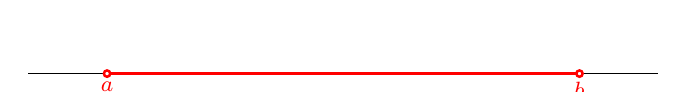
\begin{tikzpicture}
                    % \clip (0,0) rectangle (14.000000,10.000000);
                    {\footnotesize
                    
                    % Drawing line a b
                    \draw [line width=0.016cm] (1.000000,1.500000) -- (1.960000,1.500000);%
                    \draw [line width=0.016cm] (2.040000,1.500000) -- (7.960000,1.500000);%
                    \draw [line width=0.016cm] (8.040000,1.500000) -- (9.000000,1.500000);%
                    
                    % Changing color 255 0 0
                    \definecolor{r255g0b0}{rgb}{1.000000,0.000000,0.000000}%
                    \color{r255g0b0}% 
                    
                    % Drawing segment a b
                    \draw [line width=0.032cm] (2.040000,1.500000) -- (7.960000,1.500000);%
                    
                    % Marking point a by circle
                    \draw [line width=0.032cm] (2.000000,1.500000) circle (0.040000);%
                    \draw (2.000000,1.500000) node [anchor=north] { $a$ };%
                    
                    % Marking point b by circle
                    \draw [line width=0.032cm] (8.000000,1.500000) circle (0.040000);%
                    \draw (8.000000,1.500000) node [anchor=north] { $b$ };%
                    \color{black}
                    }
                    \end{tikzpicture}

                    
                Vsebuje vsa realna števila med $a$ in $b$, vključno s krajiščema $a$ in $b$.
                }
            \end{alertblock}
            }

            \only<4->{\begin{alertblock}{Odprti interval}
                \only<5->{$$ \mathbf{(a,b)=\left\{x\in\mathbb{R}; a<x<b\right\} }$$

                \centering
                    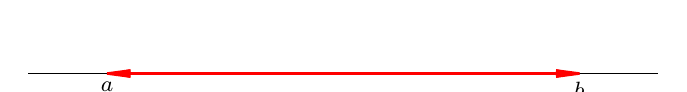
\begin{tikzpicture}
                    % \clip (0,0) rectangle (14.000000,10.000000);
                    {\footnotesize
                    
                    % Drawing line a b
                    \draw [line width=0.016cm] (1.000000,1.500000) -- (9.000000,1.500000);%
                    
                    % Changing color 255 0 0
                    \definecolor{r255g0b0}{rgb}{1.000000,0.000000,0.000000}%
                    \color{r255g0b0}% 
                    
                    % Drawing segment a b
                    \draw [line width=0.032cm] (2.000000,1.500000) -- (8.000000,1.500000);%
                    
                    % Drawing arrow a b 1.00
                    \draw [line width=0.032cm] (7.702567,1.539158) -- (8.000000,1.500000);%
                    \draw [line width=0.032cm] (7.702567,1.539158) -- (7.900856,1.500000);%
                    \draw [line width=0.032cm] (7.702567,1.460842) -- (8.000000,1.500000);%
                    \draw [line width=0.032cm] (7.702567,1.460842) -- (7.900856,1.500000);%
                    
                    % Drawing arrow b a 1.00
                    \draw [line width=0.032cm] (2.297433,1.460842) -- (2.000000,1.500000);%
                    \draw [line width=0.032cm] (2.297433,1.460842) -- (2.099144,1.500000);%
                    \draw [line width=0.032cm] (2.297433,1.539158) -- (2.000000,1.500000);%
                    \draw [line width=0.032cm] (2.297433,1.539158) -- (2.099144,1.500000);%
                    \color{black}
                        
                    % Marking point a
                    \draw (2.000000,1.500000) node [anchor=north] { $a$ };%
                    
                    % Marking point b
                    \draw (8.000000,1.500000) node [anchor=north] { $b$ };%
                    }
                    \end{tikzpicture}
 
                Vsebuje vsa realna števila med $a$ in $b$, vendar ne vsebuje krajišč $a$ in $b$.
                }
            \end{alertblock}
            }

        \end{frame}

        \begin{frame}
            
            \only<2->{\begin{alertblock}{Polodprti/polzaprti interval}
                \begin{itemize}
                    \item<3-> $$ \mathbf{[a,b)=\left\{x\in\mathbb{R}; a\leq x<b\right\} }$$
                    
                    \begin{center}
                        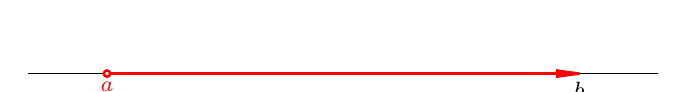
\begin{tikzpicture}
                        % \clip (0,0) rectangle (14.000000,10.000000);
                        {\footnotesize
                        
                        % Drawing line a b
                        \draw [line width=0.016cm] (1.000000,1.500000) -- (1.960000,1.500000);%
                        \draw [line width=0.016cm] (2.040000,1.500000) -- (9.000000,1.500000);%
                        
                        % Changing color 255 0 0
                        \definecolor{r255g0b0}{rgb}{1.000000,0.000000,0.000000}%
                        \color{r255g0b0}% 
                        
                        % Drawing segment a b
                        \draw [line width=0.032cm] (2.040000,1.500000) -- (8.000000,1.500000);%
                        
                        % Marking point a by circle
                        \draw [line width=0.032cm] (2.000000,1.500000) circle (0.040000);%
                        \draw (2.000000,1.500000) node [anchor=north] { $a$ };%
                        
                        % Drawing arrow a b 1.00
                        \draw [line width=0.032cm] (7.702567,1.539158) -- (8.000000,1.500000);%
                        \draw [line width=0.032cm] (7.702567,1.539158) -- (7.900856,1.500000);%
                        \draw [line width=0.032cm] (7.702567,1.460842) -- (8.000000,1.500000);%
                        \draw [line width=0.032cm] (7.702567,1.460842) -- (7.900856,1.500000);%
                        \color{black}
                        
                        % Marking point b
                        \draw (8.000000,1.500000) node [anchor=north] { $b$ };%
                        }
                        \end{tikzpicture}
                    \end{center}

                        
                    Vsebuje vsa realna števila med $a$ in $b$, vključno s krajiščem $a$, vendar ne vsebuje krajišča $b$.
                    

                    \item<4-> $$ \mathbf{(a,b]=\left\{x\in\mathbb{R}; a<x\leq b\right\} }$$
                    
                    \begin{center}
                        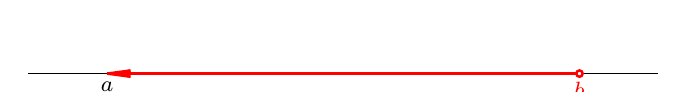
\begin{tikzpicture}
                        % \clip (0,0) rectangle (14.000000,10.000000);
                        {\footnotesize
                        
                        % Drawing line a b
                        \draw [line width=0.016cm] (1.000000,1.500000) -- (7.960000,1.500000);%
                        \draw [line width=0.016cm] (8.040000,1.500000) -- (9.000000,1.500000);%
                        
                        % Changing color 255 0 0
                        \definecolor{r255g0b0}{rgb}{1.000000,0.000000,0.000000}%
                        \color{r255g0b0}% 
                        
                        % Drawing segment a b
                        \draw [line width=0.032cm] (2.000000,1.500000) -- (7.960000,1.500000);%
                        
                        % Marking point b by circle
                        \draw [line width=0.032cm] (8.000000,1.500000) circle (0.040000);%
                        \draw (8.000000,1.500000) node [anchor=north] { $b$ };%
                        
                        % Drawing arrow b a 1.00
                        \draw [line width=0.032cm] (2.297433,1.460842) -- (2.000000,1.500000);%
                        \draw [line width=0.032cm] (2.297433,1.460842) -- (2.099144,1.500000);%
                        \draw [line width=0.032cm] (2.297433,1.539158) -- (2.000000,1.500000);%
                        \draw [line width=0.032cm] (2.297433,1.539158) -- (2.099144,1.500000);%
                        \color{black}

                        % Marking point a
                        \draw (2.000000,1.500000) node [anchor=north] { $a$ };%
                        }
                        \end{tikzpicture}
                    \end{center}

                        
                    Vsebuje vsa realna števila med $a$ in $b$, vključno s krajiščem $b$, vendar ne vsebuje krajišča $a$.

                \end{itemize}


            \end{alertblock}
            }
        \end{frame}

        \begin{frame}
            \only<2->{\begin{alertblock}{Neomejeni/neskončni intervali}
                
                \begin{itemize}
                    \item<3-> $ \mathbf{[a,\infty)=\left\{x\in\mathbb{R}; x\geq a\right\} }$ \\
                    \begin{center}
                        
\begin{tikzpicture}
                        % \clip (0,0) rectangle (14.000000,10.000000);
                        {\footnotesize
                        
                        % Drawing line a b
                        \draw [line width=0.016cm] (1.000000,1.500000) -- (1.960000,1.500000);%
                        \draw [line width=0.016cm] (2.040000,1.500000) -- (9.000000,1.500000);%
                        
                        % Changing color 255 0 0
                        \definecolor{r255g0b0}{rgb}{1.000000,0.000000,0.000000}%
                        \color{r255g0b0}% 
                        
                        % Drawing segment a y
                        \draw [line width=0.032cm] (2.040000,1.500000) -- (9.000000,1.500000);%
                        
                        % Marking point a by circle
                        \draw [line width=0.032cm] (2.000000,1.500000) circle (0.040000);%
                        \draw (2.000000,1.500000) node [anchor=north] { $a$ };%
                        \color{black}
                        }
                        \end{tikzpicture}
                    \end{center}
                        
                    \item<4-> $ \mathbf{(a,\infty)=\left\{x\in\mathbb{R}; x>a\right\} }$ \\
                    \begin{center}
                        
\begin{tikzpicture}
                        % \clip (0,0) rectangle (14.000000,10.000000);
                        {\footnotesize
                        
                        % Drawing line a b
                        \draw [line width=0.016cm] (1.000000,1.500000) -- (9.000000,1.500000);%
                        
                        % Marking point a
                        \draw (2.000000,1.500000) node [anchor=north] { $a$ };%
                        
                        % Changing color 255 0 0
                        \definecolor{r255g0b0}{rgb}{1.000000,0.000000,0.000000}%
                        \color{r255g0b0}% 
                        
                        % Drawing segment a y
                        \draw [line width=0.032cm] (2.000000,1.500000) -- (9.000000,1.500000);%
                        
                        % Drawing arrow b a 1.00
                        \draw [line width=0.032cm] (2.297433,1.460842) -- (2.000000,1.500000);%
                        \draw [line width=0.032cm] (2.297433,1.460842) -- (2.099144,1.500000);%
                        \draw [line width=0.032cm] (2.297433,1.539158) -- (2.000000,1.500000);%
                        \draw [line width=0.032cm] (2.297433,1.539158) -- (2.099144,1.500000);%
                        \color{black}
                        }
                        \end{tikzpicture}
                    \end{center}

                        
                    \item<5-> $\mathbf{(-\infty,b]=\left\{x\in\mathbb{R}; x\leq b\right\} }$ \\
                    \begin{center}
                        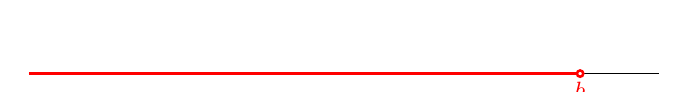
\begin{tikzpicture}
                        % \clip (0,0) rectangle (14.000000,10.000000);
                        {\footnotesize
                        
                        % Drawing line a b
                        \draw [line width=0.016cm] (1.000000,1.500000) -- (7.960000,1.500000);%
                        \draw [line width=0.016cm] (8.040000,1.500000) -- (9.000000,1.500000);%
                        
                        % Changing color 255 0 0
                        \definecolor{r255g0b0}{rgb}{1.000000,0.000000,0.000000}%
                        \color{r255g0b0}% 
                        
                        % Marking point b by circle
                        \draw [line width=0.032cm] (8.000000,1.500000) circle (0.040000);%
                        \draw (8.000000,1.500000) node [anchor=north] { $b$ };%
                        
                        % Drawing segment x b
                        \draw [line width=0.032cm] (1.000000,1.500000) -- (7.960000,1.500000);%
                        \color{black}
                        }
                        \end{tikzpicture}
                    \end{center}

                        
                    \item<6-> $ \mathbf{(-\infty,b)=\left\{x\in\mathbb{R}; x<b\right\} }$ \\
                    \begin{center}
                        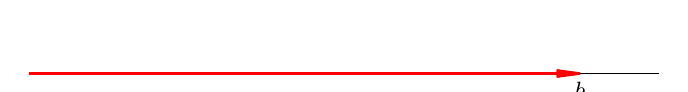
\begin{tikzpicture}
                        % \clip (0,0) rectangle (14.000000,10.000000);
                        {\footnotesize
                        
                        % Drawing line a b
                        \draw [line width=0.016cm] (1.000000,1.500000) -- (9.000000,1.500000);%
                        
                        % Marking point b
                        \draw (8.000000,1.500000) node [anchor=north] { $b$ };%
                        
                        % Changing color 255 0 0
                        \definecolor{r255g0b0}{rgb}{1.000000,0.000000,0.000000}%
                        \color{r255g0b0}% 
                        
                        % Drawing segment x b
                        \draw [line width=0.032cm] (1.000000,1.500000) -- (8.000000,1.500000);%
                        
                        % Drawing arrow a b 1.00
                        \draw [line width=0.032cm] (7.702567,1.539158) -- (8.000000,1.500000);%
                        \draw [line width=0.032cm] (7.702567,1.539158) -- (7.900856,1.500000);%
                        \draw [line width=0.032cm] (7.702567,1.460842) -- (8.000000,1.500000);%
                        \draw [line width=0.032cm] (7.702567,1.460842) -- (7.900856,1.500000);%
                        \color{black}
                        }
                        \end{tikzpicture}
                    \end{center}

                    \item<7-> $ \mathbf{(-\infty,\infty)=\left\{x;x\in\mathbb{R}\right\} =\mathbb{R}}$ \\
                    \begin{center}
                        \begin{tikzpicture}
                            % \clip (0,0) rectangle (14.000000,10.000000);
                            {\footnotesize
                            
                            % Drawing line a b
                            \draw [line width=0.016cm] (1.000000,1.500000) -- (9.000000,1.500000);%
                            
                            % Changing color 255 0 0
                            \definecolor{r255g0b0}{rgb}{1.000000,0.000000,0.000000}%
                            \color{r255g0b0}% 
                            
                            % Drawing segment x y
                            \draw [line width=0.032cm] (1.000000,1.500000) -- (9.000000,1.500000);%
                            \color{black}
                            }
                        \end{tikzpicture}
                    \end{center}

                \end{itemize}

            \end{alertblock}
            }

            \note{
                Zapis podmnožic $\mathbb{R}$ z intervali:
            \begin{itemize}
                \item $\mathbb{R}^+=(0,\infty)$
                \item $\mathbb{R}_0^+=[0,\infty)$
                \item $\mathbb{R}^-=(-\infty,0)$
            \end{itemize}
            }
        \end{frame}



        \begin{frame}
            \only<2->{\begin{exampleblock}{Naloga}
                Zapišite kot interval.
                \only<3->{\begin{itemize}
                        \item $\{x\in\mathbb{R}; -2<x<2\}$ \\~\\~
                        \item $\{x\in\mathbb{R}; 4\leq x\leq 2\}$ \\~\\~
                        \item $\{x\in\mathbb{R}; -14<x\leq -9\}$ \\~\\~
                \end{itemize}}
            \end{exampleblock}}
        \end{frame}


        \begin{frame}
            \only<2->{\begin{exampleblock}{Naloga}
                Zapišite interval, ki je narisan na sliki.
                \only<3->{\begin{itemize}
                        \item $ $ \\~\\~
                        \item $ $ \\~\\~
                        \item $ $ \\~\\~
                \end{itemize}}
            \end{exampleblock}}
        \end{frame}


        \begin{frame}
            \only<2->{\begin{exampleblock}{Naloga}
                Zapišite presek intervalov.
                \only<3->{\begin{itemize}
                    \begin{columns}
                        \column{0.4\textwidth}
                        \item $ [0,2)\cap(-1,1]$ \\~\\~
                        \item $ [-3,5]\cap(-3,5)$ \\~\\~
                        \item $ [2,5)\cap[5,7)$ \\~\\~
                        \column{0.4\textwidth}
                        \item $ [-1,3)\cap(-4,-1]$ \\~\\~
                        \item $ [4,6]\cap[-1,4]$ \\~\\~
                        \item $ (-1,3)\cap[1,2)$ \\~\\~
                    \end{columns}

                \end{itemize}}
            \end{exampleblock}}
        \end{frame}


        \begin{frame}
            \only<2->{\begin{exampleblock}{Naloga}
                Zapišite unijo intervalov.
                \only<3->{\begin{itemize}
                        \item $ [0,2)\cup(-1,1]$ \\~\\~
                        \item $ [-3,5]\cup(-3,5)$ \\~\\~
                        \item $ [2,5)\cup[5,7)$ \\~\\~
                        \item $ [-1,3)\cup(-4,1]$ \\~\\~
                \end{itemize}}
            \end{exampleblock}}
        \end{frame}


        
        \begin{frame}
            \only<2->{\begin{exampleblock}{Naloga}
                Zapišite razliko intervalov.
                \only<3->{\begin{itemize}
                        \item $ [2,3]\setminus[3,4)$ \\~\\~
                        \item $ (1,3)\setminus(3,4)$ \\~\\~
                        \item $ [2,5)\setminus(-1,2]$ \\~\\~
                        \item $ (2,8)\setminus[5,6)$ \\~\\~
                \end{itemize}}
            \end{exampleblock}}
        \end{frame}


        \begin{frame}
            \only<2->{\begin{exampleblock}{Naloga}
                Izračunajte.
                \only<3->{\begin{itemize}
                        \item $\left([1,3)\setminus(1,4]\right)\cup(1,2)$ \\~\\~
                        \item $[-2,4]\setminus\left((-1,2]\cap[0,3)\right)$ \\~\\~
                        \item $\left((-2,3]\setminus[-3,2)\right)\cap[3,5)$ \\~\\~
                \end{itemize}}
            \end{exampleblock}}
        \end{frame}


        % \begin{frame}
        %     \only<2->{\begin{exampleblock}{Naloga 423 (Linea nova)}
        %         Zapišite množico vseh neengativnih realnih števil, ki so manjša od $6$, ter iskano množico predstavite na številski premici.
        %     \end{exampleblock}
        %     \note{Rešitev N423: $\left\{x\in\mathbb{R};0\leq x<6 \right\} [0,6)$ \\}
        %     }

        %     \only<3->{\begin{exampleblock}{Naloga 585}
        %         Dana sta intervala $I=[-2,5)$ in $J=(3,6)$.
        %         \begin{itemize}
        %             % \item Intervala $I$ in $J$ nariši na številski premici.
        %             \item<4-> Zapiši $I\cap J$ in $I\cup J$.
        %             \item<5-> Izračunaj vsoto največjega celega števila iz $I$ in najmanjšega celega števila iz $J$.
        %         \end{itemize}
        %     \end{exampleblock}
        %     \note{Rešitev N585:\begin{itemize}
        %         \item $I\cap J=(3,5)$; $I\cup J=[-2,6)$
        %         \item $4+4=8$
        %     \end{itemize} }
        %     }

        %     \only<6->{\begin{exampleblock}{Naloga 583}
        %         Zapiši unijo in presek danih intervalov.
        %         \begin{description}
        %             \item[(c)]<7-> $[4,8]$ in $(3,5]$
        %             \item[(f)]<8-> $[-2,4]$ in $(2,\infty)$
        %             \item[(g)]<9-> $(-\infty,3]$ in $(-1,5]$   
        %         \end{description}
        %     \end{exampleblock}
        %     \note{Rešitev N583: \begin{description}
        %         \item[(c)] $(3,8]$ in $[4,5]$
        %         \item[(f)] $[-2,\infty)$ in $(2,4]$
        %         \item[(g)] $(-\infty,5]$ in $(-1,3]$   
        %     \end{description}
        %     }
        %     }
        % \end{frame}



    \subsection{Reševanje enačb}

        \begin{frame}
            \frametitle{Reševanje enačb}

            \only<2->{\begin{alertblock}{Enačba}
                \only<3->{\textbf{Enačba} je enakost dveh izrazov, pri čemer vsaj v enem nastopa \textbf{neznanka}, ki je ponavadi označena s črko $x$.}

                \only<4->{\textbf{Rešitev enačbe} je vsaka vrednost neznanke, za katero sta vrednosti leve in desne strani enačbe enaki.}
            \end{alertblock}}

            \only<5->{\begin{block}{Reševanje enačbe}
                \only<6->{Enačbo rešujemo tako, da jo preoblikujemo v ekvivalentno enačbo, iz katere preberemo rešitve.}

                \only<7->{Ekvivalentno enačbo dobimo, če:}
                \only<8->{\begin{itemize}
                    \item<8-> na obeh straneh enačbe prištejemo isto število ali izraz;
                    \item<9-> obe strani enačbe množimo z istim neničelnim številom ali izrazom.
                \end{itemize}}
            \end{block}}
        \end{frame}

        \begin{frame}
            \only<2->{\begin{alertblock}{Linearna enačba}
                \only<3->{\textbf{Linearna enačba} je enačba oblike $ax+b=0;~a,b\in\mathbb{R}$.}

                \only<4->{Rešujemo jo tako, da jo preoblikujemo v ekvivalentno enačbo, ki ima na eni strani samo neznanko.}
            \end{alertblock}}

            \only<5->{\begin{alertblock}{Razcepna enačba}
                \only<6->{\textbf{Razcepna enačba} je enačba, v kateri nastopajo potence neznanke (na primer $x^2$, $x^3$) in jo je mogoče zapisati kot produkt (linearnih) faktorjev.}

                \only<7->{Preoblikujemo jo v ekvivalentno enačbo, ki ima vse člene na eni strani neenačaja, na drugi pa $0$. 
                Izraz (neničelna stran) razstavimo, kolikor je mogoče, in preberemo rešitve.}
            \end{alertblock}}

            \only<8->{\begin{alertblock}{Racionalna enačba}
                \only<9->{\textbf{Racionalna enačba} je enačba, v kateri nastopajo neznake (tudi) v imenovalcu, pri tem smo pozorni na obstoj ulomkov. 
                Nato enačbo preoblikujemo v ekvivalentno enačbo.}
            \end{alertblock}}

        \end{frame}



        %%% naloge

        \begin{frame}
            \only<2->{\begin{exampleblock}{Naloga}
                Rešite enačbe.
                \only<3->{\begin{itemize}
                        \item $3(2a-1)-5(a-2)=9$ \\~\\~
                        \item $2(y-2)+3(1-y)=7$ \\~\\~
                        \item $3(3-2(t-1))=3(5-t)$ \\~\\~
                        \item $-(2-x)+3(x+1)=x-5$ \\~\\~
                \end{itemize}}
            \end{exampleblock}}
        \end{frame}


        \begin{frame}
            \only<2->{\begin{exampleblock}{Naloga}
                Rešite enačbe.
                \only<3->{\begin{itemize}
                        \item $\dfrac{1}{5}-\dfrac{x-1}{2}=\dfrac{7}{10}$ \\~\\~
                        \item $\dfrac{a-1}{3}+\dfrac{a+2}{6}=\dfrac{1}{2}$ \\~\\~
                        \item $2\dfrac{2}{3}-\dfrac{3t+1}{6}=0$ \\~\\~
                        \item $\left(\dfrac{2}{b+1}\right)^{-1}+\dfrac{b-1}{4}=b+3$ \\~
                \end{itemize}}
            \end{exampleblock}}
        \end{frame}



        \begin{frame}
            \only<2->{\begin{exampleblock}{Naloga}
                Rešite razcepne enačbe.
                \only<3->{\begin{itemize}
                        \item $x^2-3x=-2$ \\~
                        \item $(x+2)^2-(x-1)^3=8x^2+x+2$ \\~
                        \item $x^4=16x^2$ \\~
                        \item $(x^2-4x+5)^2-(x^2+4x+1)^2-78=2x^2(x+30)-18(x+1)^3$ \\~
                        \item $x^3-4x^2+4=x$ \\~
                        \item $x^5=3x^4-2x^3$ \\~
                \end{itemize}}
            \end{exampleblock}}
        \end{frame}


        \begin{frame}
            \only<2->{\begin{exampleblock}{Naloga}
                Rešite enačbe.
                \only<3->{\begin{itemize}
                        \item $\dfrac{x-1}{x+2}=\dfrac{x+1}{x-3}$ \\~\\~
                        \item $\dfrac{1}{a-1}-\dfrac{3}{a}=\dfrac{2}{a-1}$ \\~\\~
                        \item $2\dfrac{x-3}{x-2}+\dfrac{x+4}{x+1}=\dfrac{2x^2}{x^2-x-2}$ \\~\\~
                        \item $\dfrac{1}{3a-1}+\dfrac{1}{3a+1}=\dfrac{a-1}{9a^2-1}$ \\~
                \end{itemize}}
            \end{exampleblock}}
        \end{frame}


        \begin{frame}
            \only<2->{\begin{exampleblock}{Naloga}
                Neznano število smo delili s $4$ in dobljenemu količniku prišteli $1$. 
                Dobili smo enako, kot če bi istemu številu prišteli $10$. Izračunajte neznano število.
                \\~\\~\\~
            \end{exampleblock}}

            \only<3->{\begin{exampleblock}{Naloga}
                Kvadrat neznanega števila je za $4$ manjši od njegovega štirikratnika. Izračunajte neznano število.
                \\~\\~\\~
            \end{exampleblock}}

        \end{frame}


        \begin{frame}
            \only<2->{\begin{exampleblock}{Naloga}
                Avtomobil vozi s povprečno hitrostjo $50~\frac{km}{h}$, kolesar s povprečno hitrostjo $20~\frac{km}{h}$.
                Avtomobil gre iz Lendave v Ormož (približno $50~km$), kolesar vozi v obratno smer. 
                Koliko časa pred avtomobilom mora na pot kolesar, da se bosta srečala na polovici poti?
                \\~\\~\\~
            \end{exampleblock}}

            \only<3->{\begin{exampleblock}{Naloga}
                Vsota števk dvomestnega števila je $3$. Če zamenjamo njegovi števki, dobimo za $9$ manjše število. Katero število je to?
                \\~\\~
            \end{exampleblock}}

        \end{frame}


        \begin{frame}
            \only<2->{\begin{exampleblock}{Naloga}
                Andreja je bila ob rojstvu hčere Eve stara $38$ let. Čez koliko let bo Andreja stara trikrat toliko kot Eva?
                \\~\\~
            \end{exampleblock}}

            \only<3->{\begin{exampleblock}{Naloga}
                Prvi delavec sam pozida steno v  $10$ urah, drugi v $12$ urah, tretji v $8$ urah. 
                Delavci skupaj začnejo zidati steno. Po dveh urah tretji delavec odide, pridruži pa se četrti delavec. 
                Skupaj s prvim in drugim delavcem nato končajo steno v eni uri. V kolikšnem času četrti delavec pozida steno?
                \\~\\~\\~
            \end{exampleblock}}

        \end{frame}



    \subsection{Reševanje neenačb}

        \begin{frame}
            \frametitle{Reševanje neenačb}

            \only<2->{\begin{alertblock}{Neenačba}
                \only<3->{\textbf{Neenačba} je neenakost dveh izrazov, pri čemer vsaj v enem nastopa neznanka.
                Med levo in desno stranjo je postavljen eden od neenačajev: $<$, $>$, $\leq$ ali $\geq$.}
            \end{alertblock}}

            \only<4->{\begin{block}{Reševanje neenačbe}
                \only<5->{Neenačbo rešujemo tako, da jo preoblikujemo v ekvivalentno neenačbo. To dobimo, če:}
                \only<6->{\begin{itemize}
                    \item<6-> prištejemo isto število ali izraz na obeh straneh neenačbe;
                    \item<7-> množimo obe strani neenačbe z istim pozitivnim številom ali izrazom;
                    \item<8-> množimo obe strani neenačbe z istim negativnim številom ali izrazom in se pri tem neenačaj obrne.
                \end{itemize}}
            \end{block}}

            \only<9->{\begin{alertblock}{}
                \textbf{Linearna neenačba} je oblike $ax+b<0$, ali pa nastopa drug neenačaj: $>$, $\leq$, $\geq$.
            \end{alertblock}}
        \end{frame}




                %%% naloge
        
                \begin{frame}
                    \only<2->{\begin{exampleblock}{Naloga}
                        Poiščite vsa realna števila, ki ustrezajo pogoju.
                        \only<3->{\begin{itemize}
                                \item $3a+2<2a-1$ \\~\\~
                                \item $7t+8\geq 8(t-2)$ \\~\\~
                                \item $5x-2>2(x+1)-3$ \\~\\~
                                \item $x-1\leq 2(x-3)-x$ \\~\\~
                        \end{itemize}}
                    \end{exampleblock}}
                \end{frame}
        
        
                \begin{frame}
                    \only<2->{\begin{exampleblock}{Naloga}
                        Rešite neenačbe.
                        \only<3->{\begin{itemize}
                                \item $\dfrac{x}{2}+\dfrac{2}{3}<\dfrac{8}{3}$ \\~\\~
                                \item $\dfrac{4+5a}{34}-\dfrac{4}{51}\geq 2+\dfrac{2-a}{51}$ \\~\\~
                                \item $x+\dfrac{x-2}{3}<\dfrac{x-3}{4}+\dfrac{x-1}{2}$ \\~\\~
                                \item $\dfrac{2x-2}{15}+\dfrac{x}{3}<\dfrac{4x-2}{5}+\dfrac{3x+9}{10}$ \\~
                        \end{itemize}}
                    \end{exampleblock}}
                \end{frame}
        
        
        
                \begin{frame}
                    \only<2->{\begin{exampleblock}{Naloga}
                        Rešite sisteme neenačb.
                        \only<3->{\begin{itemize}
                                \item $-2<y-2<1$ \\~\\~
                                \item $-4\leq 5a-9\leq 1$ \\~\\~
                                \item $(x+1>3)\land (2x\leq 3(x-1))$ \\~\\~
                                \item $(3x-5<x+3)\lor (2x\geq x+6)$ \\~\\~
                        \end{itemize}}
                    \end{exampleblock}}
                \end{frame}
        

        % \begin{frame}
        %     \only<2->{\begin{exampleblock}{Naloga 582}
        %         Reši neenačbo in rešitev zapiši z intervalom.
        %         \begin{description}
        %             \item[(f)]<3-> $ 3-(2-2x)^2>4x(1-x) $ 
        %             \item[(l)]<4-> $ \frac{x+3}{8}\geq \frac{2x-9}{4}  $ 
        %             \item[(p)]<5-> $ \frac{x+3}{6}-\frac{2x-1}{12}\leq (3+4)^0+\frac{3x-2}{8} $ 
        %         \end{description}
        %     \end{exampleblock}
        %     \note{Rešitev N582: \begin{description}
        %         \item[(f)] $x\in(\frac{1}{4},\infty)$
        %         \item[(l)] $x\in(-\infty,7]$
        %         \item[(p)] $x\in[-\frac{4}{9},\infty)$  
        %     \end{description}}
        %     }

        %     \only<6->{\begin{exampleblock}{Naloga 584}
        %         Reši sistem neenačb in rešitev zapiši z intervalom.
        %         \begin{description}
        %             \item[(č)]<7-> $ x+4\leq 8; \quad 5-x<8 $ 
        %             \item[(h)]<8-> $ 3-(2+4x)<x^2-(2-x)^2; \quad 2-(2-x)(x+2)\geq x^2 $
        %             \item[(e)]<9-> $ 5x-3\geq 4; \quad 11-10x\geq -3 $  
        %         \end{description}
        %     \end{exampleblock}
        %     \note{Rešitev N584: \begin{description}
        %         \item[(č)] $x\in(-3,4]$
        %         \item[(h)] ni rešitve
        %         \item[(e)] $x\in\left\{\frac{7}{5}\right\}$
        %     \end{description}}
        %     }

        % \end{frame}

        % \begin{frame}
        %     \only<2->{\begin{exampleblock}{Naloga 587}
        %         Reši neenačbo $4-(2x+3)^3\geq -101-4(x+1)(2x^2+7x)$ v množici:
        %         \begin{enumerate}[a]
        %             \item realnih števil in rešitev ponazori na številski premici,
        %             \item naravnih števil in rešitev ponazori na številski premici,
        %             \item celih števil in rešitev ponazori na številski premici.
        %         \end{enumerate}
        %     \end{exampleblock}
        %     \note{Rešitev N587:\begin{enumerate}[a]
        %         \item $x\in(-\infty,3]$
        %         \item $x\in\left\{1,2,3\right\} $
        %         \item $x\in\left\{3,2,1,0,-1,-2,\dots\right\} $
        %     \end{enumerate}}
        %     }

        %     \only<3->{\begin{exampleblock}{Naloga 588}
        %         Dana sta izraza $A=3-(2x-1)^2+4x(x+2)$ in $B=2-\frac{x+1}{3}$. Za katere $x$ je:
        %         \begin{enumerate}[a]
        %             \item<4-> vrednost izraza $A$ negativna,
        %             \item<5-> vrednost izraza $B$ vsaj $-88$,
        %             \item<6-> vrednost izraza $B$ za $20$ manjša od vrednosti izraza $A$?
        %         \end{enumerate}
        %     \end{exampleblock}
        %     \note{Rešitev N588: \begin{enumerate}[a]
        %         \item $x\in(-\infty,-\frac{1}{6})$
        %         \item $x\in(-\infty,269]$
        %         \item $x\in\left\{\frac{59}{37}\right\} $
        %     \end{enumerate}}
        %     }
        % \end{frame}

    
    
    \subsection{Reševanje sistemov enačb}

        \begin{frame}
            \frametitle{Reševanje sistemov enačb}

            \only<2->{\begin{alertblock}{Sistem dveh linearnih enačb z dvema neznankama}
                \only<3->{\textbf{Sistem dveh linearnih enačb z dvema neznankama} ali \textbf{sistem $\mathbf{2\times 2}$} je v splošnem oblike:
                    $$\begin{aligned}
                            a_1x+b_1y&=c_1 \\ a_2x+b_2y&=c_2
                        \end{aligned}$$}
                \only<4->{$x$ in $y$ sta \textbf{neznanki}, $a_i,b_i,c_i\in\mathbb{R}$ so \textbf{koeficienti}.}
            \end{alertblock}}

            \only<5->{\begin{block}{}
                \textbf{Rešitev sistema} je \textbf{urejen par} števil $(x,y)$, ki zadoščajo obema enačbama.
            \end{block}}

            \only<6->{\begin{block}{}
                    Sistem $2\times 2$ ima lahko eno rešitev, nima rešitve ali ima neskončno rešitev.
            \end{block}}

        \end{frame}

        \begin{frame}
            \only<2->{\begin{block}{}
                Sistem lahko rešujemo s primerjalnim načinom, zamenjalnim načinom ali z metodo nasprotnih koeficientov.
            \end{block}}
        
            \only<3->{\begin{block}{Primerjalni način}
                Iz obeh enačb izrazimo isto neznanko, nato njuni vrednosti enačimo.
            \end{block}}

            \only<4->{\begin{block}{Zamenjalni način}
                Iz ene enačbe izrazimo eno izmed neznank (preverimo, če je kateri od koeficientov pri neznankah enak $1$ -- takšno neznanko hitro izrazimo) in izraženo vrednost vstavimo v drugo enačbo.
            \end{block}}

            \only<5->{\begin{block}{Metoda nasprotnih koeficientov}
                Eno ali obe enačbi pomnožimo s takimi števili, da bosta pri eni izmed neznank koeficienta nasprotni števili, nato enačbi seštejemo.
                Ostane ena enačba z eno neznanko.
            \end{block}}


        \end{frame}

        %%% naloge

        \begin{frame}
            \only<2->{\begin{exampleblock}{Naloga}
                Rešite sisteme enačb.
                \only<3->{\begin{itemize}
                    \begin{columns}
                        \column{0.4\textwidth}
                        \item $\begin{aligned}
                            2x+y&=9 \\ x-3y&=8
                        \end{aligned}$ \\~\\~\\~
                        \item $\begin{aligned}
                            x-y&=5 \\ y-x&=3
                        \end{aligned}$ \\~\\~\\~
                        \column{0.4\textwidth}
                        \item $\begin{aligned}
                            2x-3y&=5 \\ -4x+6y&=-10
                        \end{aligned}$ \\~\\~\\~
                        \item $\begin{aligned}
                            3x-y&=5 \\ 6x-10&=2y
                        \end{aligned}$ \\~\\~\\~
                    \end{columns}

                \end{itemize}}
            \end{exampleblock}}
        \end{frame}


        \begin{frame}
            \only<2->{\begin{exampleblock}{Naloga}
                Z zamenjalnim načinom rešite sisteme enačb.
                \only<3->{\begin{itemize}
                    \begin{columns}
                        \column{0.4\textwidth}
                        \item $\begin{aligned}
                            2x+5y&=-2 \\ x-3y&=-1
                        \end{aligned}$ \\~\\~\\~
                        \item $\begin{aligned}
                            \frac{x}{2}-y&=3 \\ y+x&=-2
                        \end{aligned}$ \\~\\~\\~
                        \column{0.4\textwidth}
                        \item $\begin{aligned}
                            3x-2y&=1 \\ x+y&=\frac{7}{6}
                        \end{aligned}$ \\~\\~\\~
                        \item $\begin{aligned}
                            0.5x+0.2y&=2 \\ \frac{3}{2}x-\frac{2}{5}y&=1
                        \end{aligned}$ \\~\\~\\~
                    \end{columns}

                \end{itemize}}
            \end{exampleblock}}
        \end{frame}


        \begin{frame}
            \only<2->{\begin{exampleblock}{Naloga}
                Z metodo nasprotnih koeficientov rešite sisteme enačb.
                \only<3->{\begin{itemize}
                    \begin{columns}
                        \column{0.4\textwidth}
                        \item $\begin{aligned}
                            2x+3y&=3 \\ -4x+3y&=0
                        \end{aligned}$ \\~\\~\\~
                        \item $\begin{aligned}
                            4x-3y&=-2 \\ -8x+y&=-1
                        \end{aligned}$ \\~\\~\\~
                        \column{0.4\textwidth}
                        \item $\begin{aligned}
                            3x-2y&=2 \\ 2x-3y&=-2
                        \end{aligned}$ \\~\\~\\~
                        \item $\begin{aligned}
                            x-y&=-5 \\ 0.6x+0.4y&=7
                        \end{aligned}$ \\~\\~\\~
                    \end{columns}

                \end{itemize}}
            \end{exampleblock}}
        \end{frame}


        \begin{frame}
            \only<2->{\begin{exampleblock}{Naloga}
                V bloku je $26$ stanovanj. Vsako stanovanje ima $2$ ali $3$ sobe. Koliko je posameznih vrst stanovanj, če je v bloku $61$ sob?
                \\~\\~\\~
            \end{exampleblock}}

            \only<3->{\begin{exampleblock}{Naloga}
                Kmet ima v ogradi $20$  živali. Če so v ogradi le race in koze, koliko je posameznih živali, če smo našteli $50$ nog? 
                \\~\\~\\~
            \end{exampleblock}}

        \end{frame}


        \begin{frame}
            \only<2->{\begin{exampleblock}{Naloga}
                Razredničarka na sladoled pelje svojih $30$ dijakov. Naročili so lahko $2$ ali $3$ kepice sladoleda. Koliko dijakov je naročilo dve in koliko tri kepice sladoleda,
                če razredničarka ni jedla sladoleda, plačala pa je $79$ kepic sladoleda?
                \\~\\~\\~
            \end{exampleblock}}

            \only<3->{\begin{exampleblock}{Naloga}
                Babica ima dvakrat toliko vnukinj kot vnukov. Vnukinjam je podarila po tri bombone, vnukom pa po štiri bombone.
                Koliko vnukinj in vnukov ima, če je podarila $70$ bombonov?
                \\~\\~\\~
            \end{exampleblock}}

        \end{frame}






        \begin{frame}
            
            \only<2->{\begin{alertblock}{Sistem treh linearnih enačb s tremi neznankami}
                \only<3->{\textbf{Sistem treh linearnih enačb z tremi neznankami} ali \textbf{sistem $\mathbf{3\times 3}$} je v splošnem oblike:
                    $$\begin{aligned}
                            a_1x+b_1y+c_1z&=d_1 \\ a_2x+b_2y+c_2z&=d_2 \\ a_3x+b_3y+c_3z&=d_3
                        \end{aligned}$$}
                \only<4->{$x$, $y$ in $z$ so \textbf{neznanke}, $a_i,b_i,c_i\in\mathbb{R}$ so \textbf{koeficienti}.}
            \end{alertblock}}

            \only<5->{\begin{block}{}
                \textbf{Rešitev sistema} je \textbf{urejena trojka} števil $(x,y,z)$, ki zadoščajo vsem trem enačbam.
            \end{block}}

            \only<6->{\begin{block}{}
                    Sistem $3\times 3$ rečujemo z istimi postopki kot sisteme $2\times 2$, le da postopek ponovimo večkrat.
            \end{block}}

        \end{frame}



        \begin{frame}
            \only<2->{\begin{exampleblock}{Naloga}
                Z metodo nasprotnih koeficientov rešite sisteme enačb.
                \only<3->{\begin{itemize}
                    \begin{columns}
                        \column{0.4\textwidth}
                        \item $\begin{aligned}
                            2x+y-3z&=5 \\ x+2y+2z&=1 \\ -x+y+z&=-4
                        \end{aligned}$ \\~\\~\\~
                        \item $\begin{aligned}
                            x-2y+6z&=5 \\ -x+3z&=-1 \\ 4y-3z&=-3
                        \end{aligned}$ \\~\\~\\~
                        \column{0.4\textwidth}
                        \item $\begin{aligned}
                            x+y-z&=0 \\ x-y-3z&=2 \\ 2x+y-3z&=1
                        \end{aligned}$ \\~\\~\\~
                        \item $\begin{aligned}
                            2x-4y+z&=3 \\ 4x-y+2z&=4 \\ -8x+2y-4z&=7
                        \end{aligned}$ \\~\\~\\~
                    \end{columns}

                \end{itemize}}
            \end{exampleblock}}
        \end{frame}


    \subsection{Obravnava enačb in neenačb}

        \begin{frame}
            \frametitle{Obravnava enačb in neenačb}

            \begin{block}{}
                Kadar v enačbi poleg neznake $x$ nastopajo tudi druge črke, na primer $a, b, c, k, l ...$, 
                le-te označujejo števila, ki imajo poljubno realno vrednost. Imenujemo jih \textbf{parametri}.
            \end{block}

            \begin{block}{}
                Vrednost parametrov vpliva na rešitev enačbe, zato moramo enačbo reševati glede na vrednosti parametrov.
                Temu postopku rečemo \textbf{obravnava enačbe}.
            \end{block}
        \end{frame}


        %%%% naloge

        \begin{frame}
            \only<2->{\begin{exampleblock}{Naloga}
                Obravnavajte enačbe.
                \only<3->{\begin{itemize}
                        \item $2(ax-3)+3=ax$ \\~\\~
                        \item $-4x-b(x-2)^2=3-bx^2-7b$ \\~\\~
                        \item $3(a-2)(x-2)=a^2(x-1)-4x+7$ \\~\\~
                        \item $(b-3)^2x-3=4x-3b$ \\~\\~
                \end{itemize}}
            \end{exampleblock}}
        \end{frame}

        \begin{frame}
            \only<2->{\begin{exampleblock}{Naloga}
                Obravnavajte neenačbe.
                \only<3->{\begin{itemize}
                        \item $a(x-2)\leq 4$ \\~\\~
                        \item $mx+4>m^2-2x$ \\~\\~
                        \item $a(a-3x+1)\geq a(x-4)+a^2x$ \\~\\~
                        \item $(k-1)^2x\leq kx+2(k+1)+5x$ \\~\\~
                \end{itemize}}
            \end{exampleblock}}
        \end{frame}






        

     
    \subsection{Sklepni račun}

        \begin{frame}
            \frametitle{Sklepni račun}

            \only<2->{\begin{block}{}
                Pri sklepnem računu obravnavamo situacije, v katerih nastopata dve količini,
                ki sta premo sorazmerni ali obratno sorazmerni.
            \end{block}}

            \only<3->{\begin{alertblock}{Premo sorazmerje}
                \only<4->{Količini $x$ in $y$ sta \textbf{premo sorazmerni}, če obstaja takšno število $k$, da je $x=k\cdot y$.}
            \end{alertblock}}

            \only<5->{\begin{alertblock}{Obratno sorazmerje}
                \only<6->{Količini $x$ in $y$ sta \textbf{obratno sorazmerni}, če obstaja takšno število $k$, da je $x=\dfrac{y}{k}$.}
            \end{alertblock}}

        \end{frame}


        %%% naloge

        \begin{frame}
            \only<2->{\begin{exampleblock}{Naloga}
                Delavec v štirih urah zasluži $10~€$. Koliko zasluži v dvanajstih urah?
                \\~\\~
            \end{exampleblock}}

            \only<3->{\begin{exampleblock}{Naloga}
                Tiskalnik v sedmih minutah natisne $42$ strani. Koliko časa potrebuje za $108$ strani?
                \\~\\~
            \end{exampleblock}}

            \only<4->{\begin{exampleblock}{Naloga}
                Tri čebele v treh dneh oprašijo devetsto cvetov. Koliko cvetov v šestih dneh opraši šest čebel?
                \\~\\~
            \end{exampleblock}}

        \end{frame}


        \begin{frame}
            \only<2->{\begin{exampleblock}{Naloga}
                Kolesar od Ljubljane do Geometrijskega središča Slovenije potuje dve uri s hitrostjo $20~km/h$. 
                Kako hitro bi moral peljati, da bi pot prevozil v eni uri in petnajstih minutah?
                \\~\\~
            \end{exampleblock}}
            
            \only<3->{\begin{exampleblock}{Naloga}
                En računalnik za pripravo posebnih efektov filma potrebuje $14$ ur.
                Koliko časa bi potrebovali trije računalniki, za pripravo posebnih efektov za šest filmov?
                \\~\\~
            \end{exampleblock}}

            \only<4->{\begin{exampleblock}{Naloga}
                Sedem pleskarjev pleska hišo $15$ dni. Po petih dneh dva delavca premestijo na drugo delovišče.
                Koliko časa bodo preostali delavci pleskali hišo?
                \\~\\~
            \end{exampleblock}}

        \end{frame}



    \subsection{Odstotni račun}

        \begin{frame}
            \frametitle{Odstotni račun}

            \begin{block}{}
                Količine pri odstotnem računu so povezane s sklepnim računim, in sicer so v premem sorazmerju.
            \end{block}

            \begin{alertblock}{}
                \textbf{Odstotek} (ali procent) $\text{\%}$ celote definiramo kot stotino celote,
                \textbf{odtisoček} (ali promil) $\permil$ kot tisočino celote.

                $$ 1~\text{\%}=\dfrac{1}{100} \quad \quad 1~\permil=\dfrac{1}{1000}$$
            \end{alertblock}

            \begin{alertblock}{}
                \textbf{Relativni delež} je kvocient med deležem in osnovo: $r=\dfrac{d}{o}$.
            \end{alertblock}

        \end{frame}

    

    \subsection{Absolutna vrednost}

        \begin{frame}
            \frametitle{Absolutna vrednost}

            \begin{columns}
                \column{0.62\textwidth}
            
            \begin{alertblock}{}
                \textbf{Absolutna vrednost} $|x|$ števila $x$ geometrijsko predstavlja oddaljenost točke, 
                ki predstavlja število $x$, od izhodišča na številski premici.
            \end{alertblock}

            \column{0.35\textwidth}
            \begin{alertblock}{}
                $$|x|=\begin{cases} x &x\geq 0; \\ -x & x<0. \end{cases}$$
            \end{alertblock}

        \end{columns}

            % \begin{block}{}
            %     $$|x|=\sqrt{x^2}$$
            % \end{block}

            \begin{block}{Lastnosti absolutne vrednosti}
                \begin{columns}
                    \column{0.44\textwidth}
                        \only<5->{\begin{itemize}
                            \item<6-> $|x|\geq 0$
                            \item<7-> $|x|=0 \Leftrightarrow x=0$
                            \item<8-> $|-x|=|x|$
                        \end{itemize}}
                    \column{0.44\textwidth}
                        \only<8->{\begin{itemize}
                            \item<8-> $|x\cdot y|=|x|\cdot|y|$
                            \item<9-> $|x+y|\leq |x|+|y|$ -- \textbf{trikotniška neenakost}
                        \end{itemize}}
                    \end{columns}
    
            \end{block}

            \begin{block}{}
                Z absolutno vrednostjo izračunamo tudi razdaljo med $x$ in $y$ kot $|x-y|$ ali $|y-x|$.
            \end{block}
        \end{frame}

    \subsection{Zaokroževanje, približki, napake}

        \begin{frame}
            \frametitle{Zaokroževanje, približki, napake}
        \end{frame}

   
\section{Pravokotni koordinatni sistem}

\begin{frame}
    \sectionpage
\end{frame}

\begin{frame}
    \tableofcontents[currentsection, hideothersubsections]
\end{frame}

    \subsection{Množice v pravokotnem koordinatnem sistemu}

        \begin{frame}
            \frametitle{Množice v pravokotnem koordinatnem sistemu}
        \end{frame}

    \subsection{Razdalja med točkama in razpolovišče daljice}

        \begin{frame}
            \frametitle{Razdalja med točkama in razpolovišče daljice}
        \end{frame}

    \subsection{Ploščina trikotnika}

        \begin{frame}
            \frametitle{Ploščina trikotnika}
        \end{frame}

    \subsection{Funkcija}

        \begin{frame}
            \frametitle{Funkcija}
        \end{frame}


\section{Funkcija}

\begin{frame}
    \sectionpage
\end{frame}

\begin{frame}
    \tableofcontents[currentsection, hideothersubsections]
\end{frame}
        
\subsection{Funkcija}
        \begin{frame}
            \frametitle{Preslikava}

            \vskip-2em
            \begin{columns}
                \column{0.73\textwidth}
                    \only<2->{\begin{alertblock}{Preslikava}
                        \only<3->{Naj bosta $\mathcal{X}$ in $\mathcal{Y}$ neprazni množici. \\} 
                        \only<4->{\textbf{Preslikava} $f$ sestoji iz:}
                        \begin{itemize}
                            \item<5-> množice $\mathcal{X}$, ki ji pravimo \textbf{domena},
                            \item<6-> množice $\mathcal{Y}$, ki ji pravimo \textbf{kodomena} in 
                            \item<7-> \textbf{prirejanja}, ki vsakemu elementu $x$ domene priredi natanko en element $y$ kodomene.
                        \end{itemize}
                    \end{alertblock}}

                \column{0.24\textwidth}

                    \only<4->{\begin{alertblock}{}
                        $$\begin{aligned}
                            f&: \only<5->{\mathcal{X}}\only<6->{\to\mathcal{Y}} \\ \only<7->{f&: x\mapsto y}
                        \end{aligned}  $$
                    \end{alertblock}}
            
        \end{columns}

        \vskip-0.4em
        \only<8->{\begin{alertblock}{}
            Elemente $x$ kodomene $\mathcal{X}$ imenujemo \textbf{originali} preslikave.
             \only<9->{\\ Če elementu $x$ priredimo element $y$ iz kodomene, potem $y$ imenujemo \textbf{slika} elemeta $x$.}
        \end{alertblock}}

        \vskip-0.4em
        \only<10->{\begin{block}{}
            Preslikavo lahko podamo s predpisom, puščičnim diagramom, besednim opisom ...
        \end{block}}

        \end{frame}


        \begin{frame}
            \frametitle{Funkcija}

            \only<2->{\begin{alertblock}{Funkcija}
                \only<3->{Naj bosta $\mathcal{X}$ in $\mathcal{Y}$ neprazni številski množici. \\}
                \only<4->{\textbf{Funkcija} $f$ je preslikava med številskima množicama $\mathcal{X}$ in $\mathcal{Y}$:}
                \vskip-0.5em
                \only<5->{$$f: \mathcal{X}\to\mathcal{Y}.$$}
            \end{alertblock}}


            \only<6->{\begin{alertblock}{}
                Število $y$ je \textbf{funkcijska vrednost} števila $x$, če se število $x$ preslika v število $y$. 
                \vskip-0.5em
                \only<6->{$$ f(x)=y $$}
            \end{alertblock}}

            \only<7->{\begin{block}{}
                $x$ je neodvisna spremenjlivka, $f(x)$ je od $x$ odvisna spremenljivka.
            \end{block}}

        \end{frame}

        
        \begin{frame}
            
            \only<2->{\begin{block}{}
                V nekaterih primerih za opis funkcije uporabimo poseben izraz:
                \begin{itemize}
                    \item<3-> $f:\mathcal{X}\to\mathbb{R}; \mathcal{X}\subseteq\mathbb{R}$ -- realna funkcija realne spremenljivke;
                    \item<4-> $f:\mathcal{X}\to\mathbb{R}; \mathcal{X}\subseteq\mathbb{N}$ -- realna funkcija naravne spremenljivke;
                    \item<5-> $f:\mathcal{X}\to\mathbb{N}; \mathcal{X}\subseteq\mathbb{R}$ -- naravna funkcija realne spremenljivke;
                    \item<6-> $f:\mathcal{X}\to\mathbb{N}; \mathcal{X}\subseteq\mathbb{N}$ -- naravna funkcija naravne spremenljivke.
                \end{itemize}
            \end{block}}
        \end{frame}

        \begin{frame}
            \frametitle{Definicijsko območje in zaloga vrednosti}

            \only<2->{\begin{alertblock}{Definicijsko območje}
                \only<3->{\textbf{Definicijsko območje} preslikave ali funkcije $f:\mathcal{X}\to\mathcal{Y}$ je množica vseh originalov, ki jih v danem primeru opazujemo. 
                Oznaka: $D_f$.    }            
            \end{alertblock}}

            \vskip-0.5em
            \only<4->{\begin{block}{}
                Za definicijsko območje navadno vzamemo največjo možno množico, za katero je predpis funkcije veljaven/definiran.
            \end{block}}

            \only<5->{\begin{alertblock}{Zaloga vrednosti}
                \only<6->{\textbf{Zaloga vrednosti} preslikave ali funkcije $f:\mathcal{X}\to\mathcal{Y}$ je množica vseh slik oziroma funkcijskih vrednosti.
                Oznaka: $Z_f$.}
            \end{alertblock}}

            \vskip-0.5em
            \only<7->{\begin{block}{}
                Zaloga vrednosti $Z_f$ je podmnožica kodomene $\mathcal{Y}$: $Z_f\subseteq \mathcal{Y}$.
            \end{block}}

        \end{frame}



        %%%% naloge

        \begin{frame}

            \only<2->{\begin{exampleblock}{Naloga}
                Funkcijo $f: A\to B$ predstavite s tabelo. Izračunajte, kam posamezna funkcija preslika $x=1$.
                \begin{itemize}
                    \item $A=\left\{-2, -1, 0, 1, 2, 3\right\}$, $B=\left\{0, 1, 2, 3, 4, 5\right\}$, $f(x)=|x|+1$ \\~
                    \item $A=\left\{1, 2, 3, 4, 5\right\}$, $B=\mathbb{N}$, $f(x)=2x+1$ \\~
                    \item $A=B=\left\{\frac{1}{3}, \frac{1}{2}, 1, 2, 3\right\}$, $f(x)=\dfrac{1}{x}$ \\~
                \end{itemize} 
            \end{exampleblock}}
           
            \only<3->{\begin{exampleblock}{Naloga}
                Tabelirajte funkcijo $g(x)=2x+|x|$ od $-3$ do $3$ s korakom $1$. \\~
            \end{exampleblock}}


        \end{frame}


        \begin{frame}
            \only<2->{\begin{exampleblock}{Naloga}
                Zapišite definicijska območja funkcij.
                \vskip-0.5em
                \begin{columns}
                    \column{0.5\textwidth}
                    \begin{itemize}
                        \item $f(x)=\dfrac{-7}{x+1}$ \\~
                        \item $g(x)=\dfrac{1}{(x+2)(x+6)}$ \\~
                        \item $h(x)=\dfrac{3x^2+1}{5}$ \\~
                        \item $i(x)=\sqrt{x-2}$ \\~
                    \end{itemize}

                    \column{0.47\textwidth}
                    \begin{itemize}
                        \item $j(x)=x^3-\frac{2}{3}$ \\~
                        \item $k(x)=\sqrt{x^2+7}$ \\~
                        \item $l(x)=\dfrac{3}{x}$ \\~
                        \item $m(x)=\dfrac{x^2+1}{x^2-5x-6}$ \\~
                    \end{itemize}
                \end{columns}

            \end{exampleblock}}
        \end{frame}

        %%%%%%%%%%%%%%%%%%%%%%%%%%%%%%%%%%%%%%%%%%%%%%%%


        \begin{frame}
            \frametitle{Ničla in začetna vrednost funkcije}

            \only<2->{\begin{alertblock}{Ničla funkcije}
                \only<3->{\textbf{Ničla} funkcije $f:\mathcal{X}\to\mathcal{Y}$ je tista vrednost $x_0\in\mathcal{X}$ neodvisne spremenljivke, 
                pri kateri je vrednost funkcije $f$ enaka $0$: $f(x_0)=0$.}
            \end{alertblock}}

            \vskip-0.5em
            \only<4->{\begin{block}{}
                Ničle funkcije $f$ poiščemo tako, da rešimo enačbo $f(x)=0$. \\
                \only<5->{Ničle so le tiste izmed vrednosti, ki ležijo v definicijskem območju $D_f$ funkcije $f$.}
            \end{block}}

            \only<6->{\begin{alertblock}{Začetna vrednost}
                \only<7->{\textbf{Začetna vrednost} funkcije $f:\mathcal{X}\to\mathcal{Y}$ je funkcijska vrednost pri $x=0$, to je $f(0)$.}
            \end{alertblock}}

            \vskip-0.5em
            \only<8->{\begin{block}{}
                Začetna vrednost obstaja le, če je $0$ v definicijskem območju funkcije $f$: $0\in D_f$.
            \end{block}}
        \end{frame}



        %%%% naloge

        \begin{frame}
            \only<2->{\begin{exampleblock}{Naloga}
                Izračunajte ničle funkcij.
                \vskip-0.5em
                \begin{columns}
                    \column{0.5\textwidth}
                    \begin{itemize}
                        \item $f(x)=\frac{4}{5}-6x$ \\~
                        \item $g(x)=x^2-7x+12$ \\~
                        \item $h(x)=\dfrac{3x+6}{5}$ \\~
                        \item $i(x)=x^2-9$ \\~
                    \end{itemize}

                    \column{0.47\textwidth}
                    \begin{itemize}
                        \item $j(x)=x^2+1$ \\~
                        \item $k(x)=x^2-3x^2-4x+12$ \\~
                        \item $l(x)=\sqrt{x+7}$ \\~
                        \item $m(x)=\dfrac{3}{x}$ \\~
                    \end{itemize}
                \end{columns}

            \end{exampleblock}}
        \end{frame}


        \begin{frame}
            \only<2->{\begin{exampleblock}{Naloga}
                Izračunajte začetne vrednosti funkcij.
                \vskip-0.5em
                \begin{columns}
                    \column{0.5\textwidth}
                    \begin{itemize}
                        \item $f(x)=\frac{4}{5}-6x$ \\~
                        \item $g(x)=x^2-7x+12$ \\~
                        \item $h(x)=\dfrac{3x+6}{5}$ \\~
                        \item $i(x)=x^2-9$ \\~
                    \end{itemize}

                    \column{0.47\textwidth}
                    \begin{itemize}
                        \item $j(x)=x^2-3x^2-4x+12$ \\~
                        \item $k(x)=\sqrt{x+7}$ \\~
                        \item $l(x)=\dfrac{3}{x}$ \\~
                        \item $m(x)=\dfrac{x^3-2x^2-4}{x^4+2x^3+3}$ \\~
                    \end{itemize}
                \end{columns}

            \end{exampleblock}}
        \end{frame}


        %%%%%%%%%%%%%%%%%%%%%%%%%%%%%%%


        \begin{frame}
            \frametitle{Graf funkcije}

            \begin{alertblock}{Graf funkcije}
                \textbf{Graf} $\Gamma_f$ funkcije $f:\mathcal{X}\to\mathcal{Y}$ je množica urejenih parov $(x,y)\in\mathcal{X}\times\mathcal{Y}$, 
                kjer element $x$ preteče celotno definicijsko območje $D_f$ funkcije, element $y$ pa je slika pripadajočega $x$, torej $y=f(x)$.
                $$ \Gamma_f=\left\{(x,y)\in\mathcal{X}\times\mathcal{Y}; x\in D_f \land y=f(x)\right\} $$
            \end{alertblock}

            \begin{block}{}
                Urejene pare iz množice $\Gamma_f$ lahko upodobimo v koordinatnem sistemu. \\
                Vsakemu elementu $(x,f(x))$ iz zgornje množice priprada natanko ena točka v koordinatnem sistemu, 
                katere abscisa je enaka $x$, ordinata pa je njegova slika $f(x)$.
            \end{block}
        \end{frame}

        %%%% naloge

        \begin{frame}
            \only<2->{\begin{exampleblock}{Naloga}
                Zapišite in narišite grafe funkcij ter zapišite začetne vrednosti in ničle, če jih funkcija ima.
                    \begin{itemize}
                        \item $f(x)=x \quad \quad D_f=\mathbb{R}$ \\~
                        \item $g(x)=-2x+1 \quad \quad D_g=\mathbb{R}$ \\~
                        \item $h(x)=x^2-1 \quad \quad D_h=\mathbb{R}$ \\~
                        \item $i(x)=\dfrac{1}{x^2} \quad \quad D_i=\left\{-2, -1, -\frac{1}{2}, \frac{1}{2}, 1, 2\right\}$ \\~
                        \item $j(x)=\dfrac{x+2}{x-3} \quad \quad D_j=\left\{-2, -1, 0, 1, 2\right\}$ \\~
                    \end{itemize}
            \end{exampleblock}}
        \end{frame}

        %%%%%%%%%%%%%%%%%%%

        \begin{frame}
            \frametitle{Naraščanje in padanje}

            \begin{alertblock}{Naraščajoča funkcija}
                Funkcija $f$ je na intervalu $(a,b)$ \textbf{naraščajoča}, če za poljubna $x_1,x_2\in(a,b); ~x_1<x_2$, velja $f(x_1)\leq f(x_2)$.
                
                Funkcija $f$ je na intervalu $(a,b)$ \textbf{strogo naraščajoča}, če za vsaka $x_1,x_2\in(a,b); ~x_1<x_2$, velja $f(x_1)<f(x_2)$.
            \end{alertblock}

            \begin{alertblock}{Padajoča funkcija}
                Funkcija $f$ je na intervalu $(a,b)$ \textbf{padajoča}, če za poljubna $x_1,x_2\in(a,b); ~x_1<x_2$, velja $f(x_1)\geq f(x_2)$.
                
                Funkcija $f$ je na intervalu $(a,b)$ \textbf{strogo padajoča}, če za vsaka $x_1,x_2\in(a,b); ~x_1<x_2$, velja $f(x_1)>f(x_2)$.
            \end{alertblock}

        \end{frame}


        %%%%%%%%%%%%

        \begin{frame}
            \frametitle{Injektivnost in surjektivnost}

        \end{frame}



        %%%%%%%%%%%%%%%%%%%%%%%%%%%%

    \subsection{Linearna funkcija}

        \begin{frame}
            \frametitle{Predpis linearne funkcije}
        \end{frame}


        %%% naloge

        \begin{frame}
            \only<2->{\begin{exampleblock}{Naloga}
                Ugotovite, ali je dana funkcija linearna. Linearnim funkcijam določite smerni koeficient in začetno vrednost.
                \vskip-0.5em
                \begin{columns}
                    \column{0.5\textwidth}
                    \begin{itemize}
                        \item $f(x)=\dfrac{1}{7x}-\dfrac{3}{4}$ \\~
                        \item $g(x)=\frac{2}{3}-\pi x$ \\~
                        \item $h(x)=\dfrac{8+6x}{24}$ \\~
                        \item $i(x)=0.\overline{3}x+1$ \\~
                    \end{itemize}

                    \column{0.47\textwidth}
                    \begin{itemize}
                        \item $j(x)=\dfrac{x^2-3}{5}$ \\~
                        \item $k(x)=-\sqrt{2}x+\frac{2}{3}$ \\~
                        \item $l(x)=2$ \\~
                    \end{itemize}
                \end{columns}

            \end{exampleblock}}
        \end{frame}



        \begin{frame}
            \only<2->{\begin{exampleblock}{Naloga}
                Zapišite predpis linearne funkcije $f$, ki ima začetno vrednost $5$ in diferenčni količnik $-3$. \\~
            \end{exampleblock}}

            \only<3->{\begin{exampleblock}{Naloga}
                Dana je linearna funkcija $f(x)=3x-4$. Izračunaj $f(-2)$, $f(0)$; $f(5)$ in $f(\sqrt{2})$. \\~
            \end{exampleblock}}

            \only<4->{\begin{exampleblock}{Naloga}
                Zapišite predpis linearne funkcije, za katero je $u(-2)=10$ in $u(0)=2$. \\~
            \end{exampleblock}}

        \end{frame}


        \begin{frame}
            \only<2->{\begin{exampleblock}{Naloga}
                Ali je funkcija naraščajoča ali padajoča?.
                \vskip-0.5em
                \begin{columns}
                    \column{0.5\textwidth}
                    \begin{itemize}
                        \item $f(x)=3x+5$ \\~
                        \item $g(x)=-2x+7$ \\~
                        \item $h(x)=10-\frac{1}{2}x$ \\~
                        \item $i(x)=\dfrac{x-1}{2}$ \\~
                    \end{itemize}

                    \column{0.47\textwidth}
                    \begin{itemize}
                        \item $j(x)=\dfrac{5-2x}{3}$ \\~
                        \item $k(x)=\dfrac{-\sqrt{3}x+1}{3}$ \\~
                        \item $l(x)=-\dfrac{2-4x}{17}$ \\~
                    \end{itemize}
                \end{columns}

            \end{exampleblock}}
        \end{frame}


        \begin{frame}
            \only<2->{\begin{exampleblock}{Naloga}
                Izračunajte ničlo linearne funkcije.
                \vskip-1.5em
                \begin{columns}
                    \column{0.5\textwidth}
                    \begin{itemize}
                        \item $f(x)=6x+12$ \\~
                        \item $g(x)=5x+2$ \\~
                        \item $h(x)=3x-12$ \\~
                        \item $i(x)=-4x+8$ \\~
                        \item $j(x)=-3x+2$ \\~
                        \item $k(x)=-x-7$ \\~
                    \end{itemize}

                    \column{0.47\textwidth}
                    \begin{itemize}
                        \item $l(x)=\frac{}{4}x-\frac{1}{4}$ \\~
                        \item $m(x)=-\dfrac{2x+3}{6}$ \\~
                        \item $n(x)=\dfrac{1-4x}{2}$ \\~
                        \item $o(x)=\dfrac{\pi x+4}{3}$ \\~
                        \item $p(x)=\sqrt{2}x+1$ \\~
                        \item $r(x)=4$ 
                    \end{itemize}
                \end{columns}

            \end{exampleblock}}
        \end{frame}



    \subsection{Predpis linearne funkcije}

        \begin{frame}
            \frametitle{Predpis linearne funkcije}
        \end{frame}


    \subsection{Graf linearne funkcije}

        \begin{frame}
            \frametitle{Graf linearne funkcije}
        \end{frame}

        
\section{Premica}

\begin{frame}
    \sectionpage
\end{frame}

\begin{frame}
    \tableofcontents[currentsection, hideothersubsections]
\end{frame}
        


    \subsection{Enačba premice}

        \begin{frame}
            \frametitle{Enačba premice}

            \begin{alertblock}{Eksplicitna oblika enačbe premice}
                $$ \mathbf{y=kx+n};~ k,n\in\mathbb{R},$$
                kjer je $k$ je \textbf{smerni koeficient}, ki ga izračunamo kot $$k=\dfrac{\Delta x}{\Delta y}=\dfrac{y_2-y_1}{x_2-x_1},$$                
                $n$ pa je \textbf{začetna vrednost}.
            \end{alertblock}

            \begin{block}{}
                Z eksplicitno obliko enačbe premice lahko zapišemo vse premice, razen tistih, ki so vzporedne ordinatni osi.
            \end{block}
        \end{frame}

        \begin{frame}
            \begin{block}{}
                Dana je premica, ki poteka skozi točki $(x_1,y_1)$ in $(x_2,y_2)$. \\
                Smerni koeficient izračunamo po formuli $$k=\dfrac{y_2-y_1}{x_2-x_1}.$$
                Iz $y_1=kx_1+n$ izrazimo $$n=y_1-kx_1$$
                in vstavimo v prvotno enačbo $$y=kx+y_1-kx_1$$
                ter preuredimo do oblike $$\mathbf{y-y_1=k(x-x_1)}.$$
            \end{block}
        \end{frame}


        \begin{frame}
            \begin{alertblock}{Odsekovna/segmentna oblika enačbe premice}
                Denimo, da premica seka koordinatni osi v točkah $M(m,0)$ in $N(0,n)$. \\
                Uporabimo eksplicitno obliko enačbe premice, v katero vstavimo znani točki
                $$y-0=\dfrac{n-0}{0-m}(x-m)$$ $$y=-\dfrac{n}{m}x+n,$$
                in  jo preoblikujemo do \textbf{odsekovne oblike enačbe premice}: 
                $$\mathbf{\dfrac{x}{m}+\dfrac{y}{n}=1}; ~m,n\in\mathbb{R}\setminus\{0\}.$$
            \end{alertblock}

            \begin{block}{}
                Vrednosti $m$ in $n$ določata \textbf{odseka}/\textbf{segmenta} na koordinatnih oseh.
            \end{block}

        \end{frame}


        \begin{frame}
            \begin{block}{}
                Z odsekovno obliko enačbe premice lahko zapišemo vse premice, razen tistih, 
                ki potekajo skozi koordinatno izhodišče $(0,0)$ ali pa so vzporedne eni od koordinatnih osi.
            \end{block}

            \begin{alertblock}{Implicitna oblika enačbe premice}
                Vsako premico lahko zapišemo z \textbf{implicitno obliko enačbe premice}:
                $$\mathbf{ax+by+c=0}; ~(a,b,c\in\mathbb{R}) \land (a~in~b~ne~hkrati~0).$$
            \end{alertblock}            
        \end{frame}


        %%%%% naloge

        \begin{frame}
            \only<2->{\begin{exampleblock}{Naloga}
                Narišite premico z dano eksplicitno obliko enačbe.
                    \begin{itemize}
                        \item $y=-2x+1$
                        \item $y=\dfrac{1}{2}x+2$
                        \item $y=2x+\dfrac{3}{4}$
                    \end{itemize}
            \end{exampleblock}}

            \only<3->{\begin{exampleblock}{Naloga}
                Narišite premico z dano odsekovno obliko enačbe.
                \vskip-1em
                \begin{columns}
                    \column{0.5\textwidth}
                    \begin{itemize}
                        \item $\dfrac{x}{3}+\dfrac{y}{5}=1$
                        \item $\dfrac{x}{2}+\dfrac{2y}{5}=1$
                    \end{itemize}

                    \column{0.47\textwidth}
                    \begin{itemize}
                        \item $\dfrac{x}{2}-\dfrac{y}{4}=1$
                        \item $\dfrac{x}{2}-\dfrac{y}{3}=-1$
                    \end{itemize}
                \end{columns}
            \end{exampleblock}}
        \end{frame}


                \begin{frame}
            \only<2->{\begin{exampleblock}{Naloga}
                Z grafa razberite ničlo in začetno vrednost ter zapišite odsekovno obliko enačbe premice.

                \begin{columns}
                    \column{0.32\textwidth}
                    \vskip-1.5em
                    \begin{figure}[H]
                        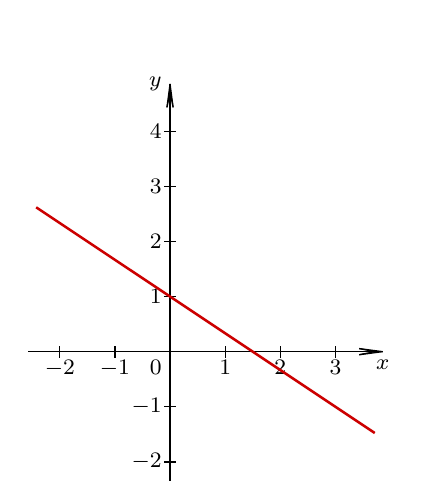
\begin{tikzpicture}
                            % \clip (0,0) rectangle (14.000000,10.000000);
                            {\footnotesize
                            
                            % Drawing 2D Cartesian system
                            \draw (3.000000,3.000000) node [anchor=north east] { $0$ };%
                            \draw [line width=0.016cm] (3.000000,2.925000) -- (3.000000,3.075000);%
                            \draw (3.700000,3.000000) node [anchor=north] { $1$ };%
                            \draw [line width=0.016cm] (3.700000,2.925000) -- (3.700000,3.075000);%
                            \draw (4.400000,3.000000) node [anchor=north] { $2$ };%
                            \draw [line width=0.016cm] (4.400000,2.925000) -- (4.400000,3.075000);%
                            \draw (5.100000,3.000000) node [anchor=north] { $3$ };%
                            \draw [line width=0.016cm] (5.100000,2.925000) -- (5.100000,3.075000);%
                            \draw (2.300000,3.000000) node [anchor=north] { $-1$ };%
                            \draw [line width=0.016cm] (2.300000,2.925000) -- (2.300000,3.075000);%
                            \draw (1.600000,3.000000) node [anchor=north] { $-2$ };%
                            \draw [line width=0.016cm] (1.600000,2.925000) -- (1.600000,3.075000);%
                            \draw (3.000000,3.700000) node [anchor=east] { $1$ };%
                            \draw [line width=0.016cm] (2.925000,3.700000) -- (3.075000,3.700000);%
                            \draw (3.000000,4.400000) node [anchor=east] { $2$ };%
                            \draw [line width=0.016cm] (2.925000,4.400000) -- (3.075000,4.400000);%
                            \draw (3.000000,5.100000) node [anchor=east] { $3$ };%
                            \draw [line width=0.016cm] (2.925000,5.100000) -- (3.075000,5.100000);%
                            \draw (3.000000,5.800000) node [anchor=east] { $4$ };%
                            \draw [line width=0.016cm] (2.925000,5.800000) -- (3.075000,5.800000);%
                            \draw (3.000000,2.300000) node [anchor=east] { $-1$ };%
                            \draw [line width=0.016cm] (2.925000,2.300000) -- (3.075000,2.300000);%
                            \draw (3.000000,1.600000) node [anchor=east] { $-2$ };%
                            \draw [line width=0.016cm] (2.925000,1.600000) -- (3.075000,1.600000);%
                            \draw (5.700000,3.000000) node [anchor=north] { $x$ };%
                            \draw (3.000000,6.400000) node [anchor=east] { $y$ };%
                            \draw [line width=0.016cm] (1.200000,3.000000) -- (5.700000,3.000000);%
                            \draw [line width=0.016cm] (5.402567,3.039158) -- (5.700000,3.000000);%
                            \draw [line width=0.016cm] (5.402567,3.039158) -- (5.600000,3.000000);%
                            \draw [line width=0.016cm] (5.402567,2.960842) -- (5.700000,3.000000);%
                            \draw [line width=0.016cm] (5.402567,2.960842) -- (5.600000,3.000000);%
                            \draw [line width=0.016cm] (3.000000,1.200000) -- (3.000000,6.400000);%
                            \draw [line width=0.016cm] (2.960842,6.102567) -- (3.000000,6.400000);%
                            \draw [line width=0.016cm] (2.960842,6.102567) -- (3.000000,6.300000);%
                            \draw [line width=0.016cm] (3.039158,6.102567) -- (3.000000,6.400000);%
                            \draw [line width=0.016cm] (3.039158,6.102567) -- (3.000000,6.300000);%
                            
                            % Changing color 204 0 0
                            \definecolor{r204g0b0}{rgb}{0.800000,0.000000,0.000000}%
                            \color{r204g0b0}% 
                            
                            % Drawing line l
                            \draw [line width=0.032cm] (1.300000,4.833220) -- (5.600000,1.966840);%
                            \color{black}
                            }
                            \end{tikzpicture}
                                                        
                    \end{figure}

                    \column{0.32\textwidth}
                    \vskip-1.5em
                    \begin{figure}[H]
                        \begin{tikzpicture}
                            % \clip (0,0) rectangle (14.000000,10.000000);
                            {\footnotesize
                            
                            % Drawing 2D Cartesian system
                            \draw (3.000000,3.000000) node [anchor=north east] { $0$ };%
                            \draw [line width=0.016cm] (3.000000,2.925000) -- (3.000000,3.075000);%
                            \draw (3.700000,3.000000) node [anchor=north] { $1$ };%
                            \draw [line width=0.016cm] (3.700000,2.925000) -- (3.700000,3.075000);%
                            \draw (4.400000,3.000000) node [anchor=north] { $2$ };%
                            \draw [line width=0.016cm] (4.400000,2.925000) -- (4.400000,3.075000);%
                            \draw (5.100000,3.000000) node [anchor=north] { $3$ };%
                            \draw [line width=0.016cm] (5.100000,2.925000) -- (5.100000,3.075000);%
                            \draw (2.300000,3.000000) node [anchor=north] { $-1$ };%
                            \draw [line width=0.016cm] (2.300000,2.925000) -- (2.300000,3.075000);%
                            \draw (1.600000,3.000000) node [anchor=north] { $-2$ };%
                            \draw [line width=0.016cm] (1.600000,2.925000) -- (1.600000,3.075000);%
                            \draw (3.000000,3.700000) node [anchor=east] { $1$ };%
                            \draw [line width=0.016cm] (2.925000,3.700000) -- (3.075000,3.700000);%
                            \draw (3.000000,4.400000) node [anchor=east] { $2$ };%
                            \draw [line width=0.016cm] (2.925000,4.400000) -- (3.075000,4.400000);%
                            \draw (3.000000,5.100000) node [anchor=east] { $3$ };%
                            \draw [line width=0.016cm] (2.925000,5.100000) -- (3.075000,5.100000);%
                            \draw (3.000000,5.800000) node [anchor=east] { $4$ };%
                            \draw [line width=0.016cm] (2.925000,5.800000) -- (3.075000,5.800000);%
                            \draw (3.000000,2.300000) node [anchor=east] { $-1$ };%
                            \draw [line width=0.016cm] (2.925000,2.300000) -- (3.075000,2.300000);%
                            \draw (3.000000,1.600000) node [anchor=east] { $-2$ };%
                            \draw [line width=0.016cm] (2.925000,1.600000) -- (3.075000,1.600000);%
                            \draw (5.700000,3.000000) node [anchor=north] { $x$ };%
                            \draw (3.000000,6.400000) node [anchor=east] { $y$ };%
                            \draw [line width=0.016cm] (1.200000,3.000000) -- (5.700000,3.000000);%
                            \draw [line width=0.016cm] (5.402567,3.039158) -- (5.700000,3.000000);%
                            \draw [line width=0.016cm] (5.402567,3.039158) -- (5.600000,3.000000);%
                            \draw [line width=0.016cm] (5.402567,2.960842) -- (5.700000,3.000000);%
                            \draw [line width=0.016cm] (5.402567,2.960842) -- (5.600000,3.000000);%
                            \draw [line width=0.016cm] (3.000000,1.200000) -- (3.000000,6.400000);%
                            \draw [line width=0.016cm] (2.960842,6.102567) -- (3.000000,6.400000);%
                            \draw [line width=0.016cm] (2.960842,6.102567) -- (3.000000,6.300000);%
                            \draw [line width=0.016cm] (3.039158,6.102567) -- (3.000000,6.400000);%
                            \draw [line width=0.016cm] (3.039158,6.102567) -- (3.000000,6.300000);%
                            
                            % Changing color 204 0 0
                            \definecolor{r204g0b0}{rgb}{0.800000,0.000000,0.000000}%
                            \color{r204g0b0}% 
                            
                            % Drawing line l
                            \draw [line width=0.032cm] (2.700000,1.300000) -- (5.600000,4.200000);%
                            \color{black}
                            }
                            \end{tikzpicture}
                            
                    \end{figure}

                    \column{0.32\textwidth}
                    \vskip-1.5em
                    \begin{figure}[H]
                        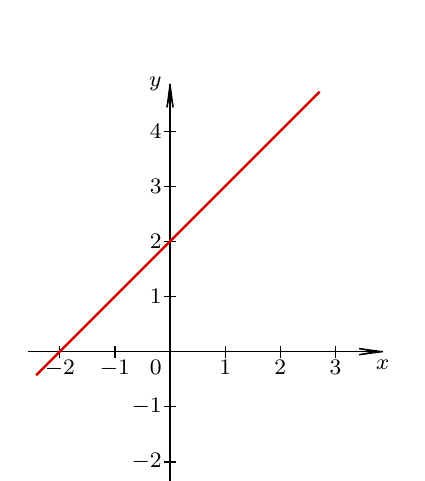
\begin{tikzpicture}
                            % \clip (0,0) rectangle (14.000000,10.000000);
                            {\footnotesize
                            
                            % Drawing 2D Cartesian system
                            \draw (3.000000,3.000000) node [anchor=north east] { $0$ };%
                            \draw [line width=0.016cm] (3.000000,2.925000) -- (3.000000,3.075000);%
                            \draw (3.700000,3.000000) node [anchor=north] { $1$ };%
                            \draw [line width=0.016cm] (3.700000,2.925000) -- (3.700000,3.075000);%
                            \draw (4.400000,3.000000) node [anchor=north] { $2$ };%
                            \draw [line width=0.016cm] (4.400000,2.925000) -- (4.400000,3.075000);%
                            \draw (5.100000,3.000000) node [anchor=north] { $3$ };%
                            \draw [line width=0.016cm] (5.100000,2.925000) -- (5.100000,3.075000);%
                            \draw (2.300000,3.000000) node [anchor=north] { $-1$ };%
                            \draw [line width=0.016cm] (2.300000,2.925000) -- (2.300000,3.075000);%
                            \draw (1.600000,3.000000) node [anchor=north] { $-2$ };%
                            \draw [line width=0.016cm] (1.600000,2.925000) -- (1.600000,3.075000);%
                            \draw (3.000000,3.700000) node [anchor=east] { $1$ };%
                            \draw [line width=0.016cm] (2.925000,3.700000) -- (3.075000,3.700000);%
                            \draw (3.000000,4.400000) node [anchor=east] { $2$ };%
                            \draw [line width=0.016cm] (2.925000,4.400000) -- (3.075000,4.400000);%
                            \draw (3.000000,5.100000) node [anchor=east] { $3$ };%
                            \draw [line width=0.016cm] (2.925000,5.100000) -- (3.075000,5.100000);%
                            \draw (3.000000,5.800000) node [anchor=east] { $4$ };%
                            \draw [line width=0.016cm] (2.925000,5.800000) -- (3.075000,5.800000);%
                            \draw (3.000000,2.300000) node [anchor=east] { $-1$ };%
                            \draw [line width=0.016cm] (2.925000,2.300000) -- (3.075000,2.300000);%
                            \draw (3.000000,1.600000) node [anchor=east] { $-2$ };%
                            \draw [line width=0.016cm] (2.925000,1.600000) -- (3.075000,1.600000);%
                            \draw (5.700000,3.000000) node [anchor=north] { $x$ };%
                            \draw (3.000000,6.400000) node [anchor=east] { $y$ };%
                            \draw [line width=0.016cm] (1.200000,3.000000) -- (5.700000,3.000000);%
                            \draw [line width=0.016cm] (5.402567,3.039158) -- (5.700000,3.000000);%
                            \draw [line width=0.016cm] (5.402567,3.039158) -- (5.600000,3.000000);%
                            \draw [line width=0.016cm] (5.402567,2.960842) -- (5.700000,3.000000);%
                            \draw [line width=0.016cm] (5.402567,2.960842) -- (5.600000,3.000000);%
                            \draw [line width=0.016cm] (3.000000,1.200000) -- (3.000000,6.400000);%
                            \draw [line width=0.016cm] (2.960842,6.102567) -- (3.000000,6.400000);%
                            \draw [line width=0.016cm] (2.960842,6.102567) -- (3.000000,6.300000);%
                            \draw [line width=0.016cm] (3.039158,6.102567) -- (3.000000,6.400000);%
                            \draw [line width=0.016cm] (3.039158,6.102567) -- (3.000000,6.300000);%
                            
                            % Changing color 204 0 0
                            \definecolor{r204g0b0}{rgb}{0.800000,0.000000,0.000000}%
                            \color{r204g0b0}% 
                            
                            % Drawing line l
                            \draw [line width=0.032cm] (4.900000,6.300000) -- (1.300000,2.700000);%
                            \color{black}
                            }
                            \end{tikzpicture}
                            
                    \end{figure}

                \end{columns}

            \end{exampleblock}}

        \end{frame}


        \begin{frame}
            \only<2->{\begin{exampleblock}{Naloga}
                Dano enačbo premice zapišite v eksplicitni in odsekovni obliki ter premico narišite.
                \vskip-1em
                \begin{columns}
                    \column{0.5\textwidth}
                    \begin{itemize}
                        \item $x+4y-8=0$
                        \item $3x-2y+6=0$
                        \item $2x+5y+5=0$
                    \end{itemize}

                    \column{0.47\textwidth}
                    \begin{itemize}
                        \item $\dfrac{1}{2}x+3y-6=0$
                        \item $x+1=0$
                        \item $y-2=0$ \\~
                    \end{itemize}
                \end{columns}

            \end{exampleblock}}

            \only<3->{\begin{exampleblock}{Naloga}
                Izračunajte ploščino trikotnika, ki jo premica oklepa s koordinatnima osema.
                \vskip-1em
                \begin{columns}
                    \column{0.5\textwidth}
                    \begin{itemize}
                        \item $y=-2x+4$
                        \item $\dfrac{x}{2}+\dfrac{x}{-3}=1$
                    \end{itemize}

                    \column{0.47\textwidth}
                    \begin{itemize}
                        \item $2x+4y-3=0$
                        \item $x-y+1=0$ \\~
                    \end{itemize}
                \end{columns}
            \end{exampleblock}}

        \end{frame}


        \begin{frame}
            \only<2->{\begin{exampleblock}{Naloga}
                Zapišite enačbo premice, ki gre skozi dani točki.
                    \begin{itemize}
                        \item $A(2,3)$ in $B(4,5)$ 
                        \item $C(1,-2)$ in $D(-3,-4)$ 
                        \item $E(7,2)$ in $F(-7,-5)$ \\~
                    \end{itemize}
            \end{exampleblock}}

            \only<3->{\begin{exampleblock}{Naloga}
                Določite neznano koordinato tako, da bodo dane točke kolinearne.
                    \begin{itemize}
                        \item $A(3,y)$, $B(-4,1)$ in $C(2,2)$ 
                        \item $D(-1,7)$, $E(x,5)$ in $F(3,-4)$ \\~
                    \end{itemize}
            \end{exampleblock}}

        \end{frame}


        \begin{frame}
            \only<2->{\begin{exampleblock}{Naloga}
                Ugotovite, ali sta dani premici vzporedni.
                    \begin{itemize}
                        \item $y=\dfrac{3}{4}x-1$ in $y=-\dfrac{3}{4}x+1$ \\~
                        \item $x-2y+1=0$ in $2x+y+1=0$ \\~
                        \item $\dfrac{x}{3}-\dfrac{y}{6}=1$ in $\dfrac{x}{2}+\dfrac{y}{4}=1$ \\~
                        \item $\dfrac{x}{4}+\dfrac{y}{2}=1$ in $4x+2y+1=0$ \\~

                    \end{itemize}
            \end{exampleblock}}


        \end{frame}


        \begin{frame}
            
            \only<2->{\begin{exampleblock}{Naloga}
                Dani sta premici z enačbama $y=4x+9$ in $ax-3y+3=0$. Določite parameter $a$ tako, da bosta premici vzporedni.
            \end{exampleblock}}

            \only<3->{\begin{exampleblock}{Naloga}
                Dani sta premici z enačbama $\dfrac{x}{2}-\dfrac{y}{7}=1$ in $-6x+by+1=0$. Določite parameter $b$ tako, da bosta premici vzporedni.
            \end{exampleblock}}

            \only<4->{\begin{exampleblock}{Naloga}
                Dani sta premici z enačbama $3x-2y+4=0$ in $(c-2)x+4y+3=0$. Določite parameter $c$ tako, da bosta premici vzporedni.
            \end{exampleblock}}

        \end{frame}


        \begin{frame}
            \only<2->{\begin{exampleblock}{Naloga}
                Zapišite enačbo premice, ki je vzporedna dani premici in poteka skozi dano točko.
                    \begin{itemize}
                        \item $y=2x-1$, $T(1,-3)$ 
                        \item $2x-4y+3=0$, $U(-4,5)$ 
                        \item $\dfrac{x}{4}+\dfrac{y}{8}=1$, $V(8,-8)$ \\~

                    \end{itemize}
            \end{exampleblock}}


            \only<3->{\begin{exampleblock}{Naloga}
                Iz snopa premic z enačbo $y=-3x+n$ določite enačbo tiste premice, ki poteka skozi točko $(1,4)$.
            \end{exampleblock}}

            \only<4->{\begin{exampleblock}{Naloga}
                Iz šopa premic z enačbo $y=kx+2$ določite enačbo tiste premice, ki gre skozi točko $(3,-4)$.
            \end{exampleblock}}

        \end{frame}


        \begin{frame}
            \only<2->{\begin{exampleblock}{Naloga}
                Zapišite enačbo pravokotnice na dano premico, ki poteka skozi dano točko.
                    \begin{itemize}
                        \item $y=x+2$, $T(3,-4)$ \\~
                        \item $y=2x+3$, $U(4,5)$ \\~
                        \item $y=\dfrac{1}{3}x+5$, $V(-1,4)$ \\~
                        \item $y=-\dfrac{2}{3}x+\dfrac{4}{5}$, $Z(-6,3)$ \\~

                    \end{itemize}
            \end{exampleblock}}

        \end{frame}




    \subsection{Presečišče premic}

        \begin{frame}
            \frametitle{Presečišče premic}
        \end{frame}


        \begin{frame}
            \only<2->{\begin{exampleblock}{Naloga}
                Izračunajte presečišče premic, rezultat preverite s sliko.
                \begin{itemize}
                    \begin{columns}
                        \column{0.4\textwidth}
                        \item $\begin{aligned}
                            2x-3x-3&=0 \\ x&=3
                        \end{aligned}$ \\~\\~
                        \item $\begin{aligned}
                            y&=3x+3 \\ y&=\dfrac{x}{2}+3
                        \end{aligned}$ \\~

                        \column{0.4\textwidth}
                        \item $\begin{aligned}
                            x+3y-9&=0 \\ x-3y-3&=0
                        \end{aligned}$ \\~\\~
                        \item $\begin{aligned}
                            \dfrac{x}{3}-\dfrac{y}{6}&=1 \\ \dfrac{x}{2}+\dfrac{y}{5}&=1
                        \end{aligned}$ \\~
                    \end{columns}

                \end{itemize}
            \end{exampleblock}}
        \end{frame}


        \begin{frame}
            
            \only<2->{\begin{exampleblock}{Naloga}
                Zapišite enačbo premice, ki gre skozi presečišče premic $y=2x+1$ in $y=-\frac{1}{2}x+6$ ter seka ordinatno os pri $y=4$.
            \end{exampleblock}}

            \only<3->{\begin{exampleblock}{Naloga}
                Zapišite enačbo premice, ki gre skozi presečišče premic $y=3x+1$ in $y=-x+5$ ter ima smerni koeficient $k=2$.
            \end{exampleblock}}

            \only<4->{\begin{exampleblock}{Naloga}
                Zapišite implicitno enačbo premice, ki gre skozi presečišče premic $2x-y-13=0$ in $2x+3y-1=0$ ter seka abscisno os pri $x=\frac{7}{2}$.
            \end{exampleblock}}

        \end{frame}


        \begin{frame}
            
            \only<2->{\begin{exampleblock}{Naloga}
                Zapišite enačbo premice, ki gre skozi presečišče premic $3x+4y-11=0$ in $2x-7y+41=0$ ter je vzporedna ordinatni osi.
            \end{exampleblock}}

            \only<3->{\begin{exampleblock}{Naloga}
                Zapišite eksplicitno enačbo premice, ki gre skozi presečišče premic $5x-7y+3=0$ in $2x+y-14=0$ ter je vzporedna premici z enačbo $3x-2y+1=0$.
            \end{exampleblock}}

            \only<4->{\begin{exampleblock}{Naloga}
                Izračunajte smerni koeficient $k$ tako, da se premici z enačbama $y=2x+6$ in $y=kx+\frac{5}{2}$ sekata na simetrali sodih kvadrantov.
            \end{exampleblock}}

        \end{frame}


        \begin{frame}
            
            \only<2->{\begin{exampleblock}{Naloga}
                Stranice trikotnika ležijo na premicah z enačbami $x+y=0$, $3x-2y=0$ in $x-4y+10=0$. 
                Izračunajte oglišča trikotnika ter njegov obseg in ploščino.
                Premice in trikotnik narišite v pravokotnem koordinatnem sistemu.
            \end{exampleblock}}

            \only<3->{\begin{exampleblock}{Naloga}
                Dani sta dve oglišči $A$ in $B$ trikotnika $\triangle ABC$, orientacija in ploščina. Izračunajte kooridnati tretjega oglišča $C$, če leži na dani premici.
                \begin{itemize}
                    \item $A(-6,1)$, $B(2,-1)$; \\ pozitivna orientacija, $S=25$; \\ $C$ leži na $y=-2x+4$
                    \item $A(-4,0)$, $B(4,2)$; \\ pozitivna orientacija, $S=7$; \\ $C$ leži na $y=5-2x$
                \end{itemize}
            \end{exampleblock}}


        \end{frame}




\section{Statistika}

\begin{frame}
    \sectionpage
\end{frame}

\begin{frame}
    \tableofcontents[currentsection, hideothersubsections]
\end{frame}


    \subsection{Osnovni pojmi statistike}

        \begin{frame}
            \frametitle{Osnovni pojmi statistike}

            \begin{alertblock}{}
                \textbf{Populacija} je množica, ki jo statistično proučujemo. 
                Element populacije imenujemo \textbf{statistična enota}. 
            \end{alertblock}
            
            \begin{alertblock}{}
                \textbf{Vzorec} je podmnožica populacije, katere elementi predstavljajo največjo možno mero značilnosti celotne množice. 
                Vzorec izberemo, kadar je celotna populacija prevelika množica, da bi analizirali vse njene elemente. \\
                
                \begin{itemize}
                    \item \textbf{Reprezentativen vzorec} je vzorec, ki je izbran tako, da predstavlja značilnosti celotne populacije.
                    \item \textbf{Slučajni vzorec} je vzorec, ki je izbran naključno -- vsi elementi populacije imajo enako možnost, da bodo izbrani.
                \end{itemize}

                \textbf{Numerus} je število elementov vzorca. Oznaka $N$. 
            \end{alertblock}

        \end{frame}    


        \begin{frame}
            \begin{alertblock}{}
                \textbf{Statistična spremenljivka/podatek/znak} je vrednost ali lastnost, ki jo proučujemo.
            \end{alertblock}

            \begin{alertblock}{Vrste statističnih spremenljivk}
                \begin{itemize}
                    \item \textbf{opisne/kvalitativne} statistične spremenljivke
                    \item \textbf{vrstne/ordinalne} statistične spremenljivke
                    \item \textbf{številske/kvantitivne} statistične spremenljivke
                \end{itemize}
                
            \end{alertblock}

            \begin{block}{Številske statistične spremenljivke}
                \begin{itemize}
                    \item \textbf{diskretne} številske spremenljivke -- zavzamejo lahko posamezne vrednosti
                    \item \textbf{zvezne} številske spremenljivke -- zavzamejo lahko vsako vrednost z nekega intervala
                \end{itemize}

            \end{block}


        \end{frame}


        %%%% naloge

        \begin{frame}
            \only<2->{\begin{exampleblock}{Naloga}
                Zapišite, kaj je v danem primeru populacija, vzorec, statistična enota, spremenljivka in 
                ugotovite ali je spremenljivka opisna ali numerična in, če je numerična, ugotovite, ali je zvezna ali diskretna.
                \only<3->{\begin{itemize}
                        \item Na spletni strani je anketa z vprašanjem ``Ali imate doma pomivalni stroj?''. Nanjo je odgovorilo $254$ ljudi. 
                        \item V televizijski oddaji gledalci glasujejo za dva kandidata. 
                        \item Razrednik svojih $28$ dijakov vpraša, kolikšna je oddaljenost njihovega doma do šole.
                        \item Maturant piše seminarsko nalogo z naslovom ``Uporaba TikTok-a med srednješolci''. Pridobil je odgovore $369$ srednješolcev, ki so odgovarjali na vprašanje ``Ali~uporabljaš~TikTok?'' 
                        \item Znanstveniki pri raziskavi spremljajo, koliko jajc znesejo kokoši na slovenskih farmah na mesec.
                \end{itemize}}
            \end{exampleblock}}
        \end{frame}

        \begin{frame}

                \begin{columns}
                    \column{0.45\textwidth}


            \only<2->{\begin{exampleblock}{Naloga}
                    Slovenija ima več kot $6000$ naselij. Statistični urad Republike Slovenije je januarja 2024 naredil analizo naselij glede na število prebivalcev. 
                    Rezultati so prikazani v tabeli. \\~
                    
                    \only<4->{Zapišite, kaj je v danem primeru populacija, statistična enota, spremenljivka in ugotovite ali je spremenljivka opisna ali numerična in, 
                    če je numerična, ugotovite ali je zvezna ali diskretna.}
            \end{exampleblock}}

                    \column{0.5\textwidth}
                    \only<3->{\begin{table}
                        \centering
                        \begin{tabular}{||c|c||} 
                        \hhline{|t:==:t|}
                        \rowcolor[rgb]{0.843,0.718,0.718} 
                        velikostni razred naselja  & število naselij   \\ 
                        \hhline{|:==:|}
                        $0$ & $57$    \\ 
                        \hline
                        $1-24$ & $719$    \\ 
                        \hline
                        $25-49$ & $851$    \\ 
                        \hline
                        $50-99$ & $1256$     \\
                        \hline
                        $100-199$ & $1444$     \\
                        \hline
                        $200-499$ & $1109$     \\
                        \hline
                        $500-999$ & $359$     \\
                        \hline
                        $1000-4999$ & $199$     \\
                        \hline
                        $5000-9999$ & $23$     \\
                        \hline
                        $10000-49999$ & $16$     \\                    
                        \hline
                        $50000+$ & $2$     \\
                        \hhline{|b:==:b|}
                        \end{tabular}
                    \end{table}}
                \end{columns}
                
        \end{frame}



    \subsection{Urejanje in grupiranje podatkov}

        \begin{frame}
            \frametitle{Urejanje in grupiranje podatkov}

            \begin{block}{}
                Podatke, pridobljene v posamezni raziskavi, moramo najprej urediti. \\
                Če podatkov ni veliko, jih uredimo po velikosti v \textbf{ranžirno vrsto}, sicer jih združujemo v skupine, \textbf{frekvenčne razrede}.
            \end{block}

            \begin{block}{}
                Podatek z največjo vrednostjo označimo z $x_{max}$, podatek z najnižjo vrednostjo pa $x_{min}$.
            \end{block}

            \begin{alertblock}{}
                \textbf{Frekvenca} $f$ statističnega znaka je posamezno število diskretnih statističnih enot iste vrednosti.
            \end{alertblock}

            \begin{alertblock}{}
                \textbf{Frekvenčni razred} je skupina podatkov iz vzorca. Frekvenčni razredi so navadno enako široki,
                in skupaj zajamejo celoten razpon podatkov. Za zvezen nabor podatkov za frekvenčne razrede izberemo intervale (navadno oblike $[a,b)$).
            \end{alertblock}

        \end{frame}

        \begin{frame}
            \begin{alertblock}{}
                \textbf{Širina frekvenčnega razreda} $d_k$ je razlika med zgornjo ($z_k$) in spodnjo ($s_k$) mejo frekvenčnega razreda:
                $$d_k=z_k-s_k.$$
            \end{alertblock}

            \begin{block}{}
                Če so razredi enako široki, določimo njihovo širino kot kvocient med celotnim razponom podatkov $x_{max}-x_{min}$ in številom razredov.
            \end{block}

            \begin{alertblock}{}
                \textbf{Sredina frekvenčnega razred} $x_k$ je aritmetična sredina zogrnje in spodnje meje razreda: 
                $$x_k=\dfrac{z_k+s_k}{2}.$$
            \end{alertblock}
        \end{frame}

        \begin{frame}
            \begin{alertblock}{}
                Grupirane podatke predstavimo s \textbf{frekvenčno preglednico/porazdelitvijo}.
            \end{alertblock}

            \begin{alertblock}{}
                Za podatke v frekvenčnih preglednicah računamo:
                \begin{itemize}
                    \item \textbf{(absolutno) frekvenco} $f_k$ -- število podatkov z vrednostmi v danem frekvenčnem razredu;
                    \item \textbf{relativno frekvenco} $f_k'$ -- delež celote, ki ga predstavlja število podatkov v danem frekvenčnem razredu;
                    \item \textbf{(absolutno) kumulativno frekvenco} $F_k$ -- število podatkov, katerih vrednosti zavzemajo manjšo vrednost od zgornje meje danega frekvenčnega razreda;
                    \item \textbf{relativno kumulativno frekvenco} $F_k'$ -- delež celote, ki ga predstavlja število podatkov v danem in vseh manjših frekvenčnih razredih.
                \end{itemize}
            \end{alertblock}
        \end{frame}



                %%%% naloge

        
                \begin{frame}
        
                        \begin{columns}
                            \column{0.5\textwidth}
        
        
                    \only<2->{\begin{exampleblock}{Naloga}
                        Na šoli analizirajo količino prevzetih obrokov v jedilnici. Rezultati so zbrani v tabeli. \\
                        \only<4->{Analizirajte podatke s frekvenčno preglednico.
                        Podatke razdelite v razrede $5-9$, $10-14$, $15-19$, $20$ in več.}
                    \end{exampleblock}}
        
                            \column{0.45\textwidth}
                            \only<3->{\begin{table}
                                \centering
                                \begin{tabular}{||c|c||} 
                                \hhline{|t:==:t|}
                                \rowcolor[rgb]{0.843,0.718,0.718} 
                                Oddelek  & Število prevzetih obrokov   \\ 
                                \hhline{|:==:|}
                                1.a & $12$    \\ 
                                \hline
                                1.b & $14$    \\ 
                                \hline
                                1.c & $20$    \\ 
                                \hline
                                2.a & $17$     \\
                                \hline
                                2.b & $16$     \\
                                \hline
                                2.c & $9$     \\
                                \hline
                                3.a & $13$     \\
                                \hline
                                3.b & $16$     \\
                                \hline
                                3.c & $14$     \\
                                \hline
                                4.a & $21$     \\                    
                                \hline
                                4.b  & $8$     \\
                                \hline
                                4.c  & $12$     \\
                                \hhline{|b:==:b|}
                                \end{tabular}
                            \end{table}}
                        \end{columns}
                        
                \end{frame}

                
                \begin{frame}
                    \only<2->{\begin{exampleblock}{Naloga}
                        Dijaki 3. a oddelka so zapisovali svoje pribljubljene barve. \\
                        Zapisali so jih: modra, rdeča, rdeča, zelena, rumena, rdeča, modra, zelena, modra, modra, rumena, rdeča, zelena, modra, rumena, rumena, zelena, rdeča. \\
                        Analizirajte rezultate s frekvenčno preglednico. \\~\\~
                    \end{exampleblock}}

                    \only<3->{\begin{exampleblock}{Naloga}
                        Lokostrelec si beleži rezultate treningov. \\
                        Vrednosti so bile: $10.3$, $10.4$, $9.9$, $9.7$, $10.2$, $8.9$, $9.4$, $10.1$, $9.0$, $10.3$, $9.5$, $10.6$. \\
                        Analizirajte rezultate s frekvenčno preglednico. \\~\\~
                    \end{exampleblock}}
                \end{frame}

                \begin{frame}
        
                   \only<2->{\begin{exampleblock}{Naloga}
                    
                    V frekvenčni preglednici so zbrani podatki o številu sorojencev dijakov 2.~b oddelka.
                    Dopolnite preglednico.
    
                        \begin{table}
                            \centering
                            \begin{tabular}{||c|c|c|c|c||} 
                            \hhline{|t:=====:t|}
                            \rowcolor[rgb]{0.843,0.718,0.718} 
                            Število sorojencev  & $f_k$ & $f_k'$ & $F_k$ & $F_k'$   \\ 
                            \hhline{|:=====:|}
                            0 & $5$  & & &  \\ 
                            \hline
                            1 & & $25~\%$ & &    \\ 
                            \hline
                            2 & & & &    \\ 
                            \hline
                            3 & & $10~\%$ & &   \\
                            \hline
                            skupaj & $20$ & $100~\%$ & / & /    \\
                            \hhline{|b:=====:b|}
                            \end{tabular}
                        \end{table}
                    \end{exampleblock}}
    
            \end{frame}


    \subsection{Mere osredinjenosti}

        \begin{frame}
            \frametitle{Mere osredinjenosti}

            \begin{alertblock}{Aritmetična sredina}
                \textbf{Aritmetična sredina} ali \textbf{povprečje} je količnik vsote vseh vrednosti 
                statistične spremenljivke in števila teh vrednosti. \\

                $$\overline{x}=\dfrac{x_1+x_2+\cdots+x_n}{N}=\dfrac{1}{N}\sum_{i=1}^n x_i.$$
            % \end{alertblock}                
            % \begin{block}{}
                Če se vrednosti statistične spremenljivke ponavljajo ($k_i$ vrednosti $x_i$), je formula sledeča:
                $$\overline{x}=\dfrac{k_1x_1+k_2x_2+\cdots+k_mx_m}{k_1+k_2+\cdots+k_m}=\dfrac{\sum_{i=1}^mk_ix_i}{\sum_{i=1}^mk_i}; \quad \sum_{i=1}^mk_i=N$$
  
            \end{alertblock}   

            \begin{block}{}
                Pri grupiranih podatkih za vrednosti vzamemo sredine frekvenčnih razredov.
            \end{block}

        \end{frame}

        \begin{frame}
            \begin{alertblock}{Modus}
                \textbf{Modus} ali \textbf{gostiščnica $Mo$} je vrednost statistične spremenljivke, ki se v množici vseh vrednosti najpogosteje ponavlja.                 
            \end{alertblock}

            \begin{block}{}
                Če se v neki množici dve vrednosti pojavita enako mnogokrat najpogosteje, rečemo, da je porazdelitev vrednosti \textbf{bimodalna}.
            \end{block}

            \begin{block}{}
                Za grupirane podatke določamo \textbf{modalni razred}, to je tisti razred, ki ima največjo frekvenčno gostoto.
            \end{block}
        \end{frame}

        \begin{frame}
            \begin{alertblock}{Mediana}
                \textbf{Mediana} ali \textbf{središčnica $Me$} je tista vrednost statistične spremenljivke, pri kateri je polovica vrednosti večjih ali enakih,
                druga polovica vrednosti pa manjših ali enakih od te vrednosti.                 
            \end{alertblock}

            \begin{block}{}
                Če imamo liho število vrednosti statistične spremenljivke, za mediano vzamemo vrednost, ki stoji na mestu $\frac{n+1}{2}$ po velikosti urejenih podatkov. \\
                Če je število vrednosti sodo, za vrednost mediane vzamemo aritmetično sredino srednjih dveh podatkov.
            \end{block}

            \begin{block}{}
                Mediana razdeli podatke na dve polovici. Ti dve polovici lahko spet razdelimo na dve polovici in dobimo štiri enako močne množice podatkov. 
                Meje teh skupin imenujemo \textbf{kvartili}.
            \end{block}
        \end{frame}

        \begin{frame}
            \begin{block}{Kvartili}
                \textbf{Prvi kvartil $Q_1$} je mediana prve (spodnje) polovice podatkov, \textbf{drugi kvartil $Q_2$} je mediana $Me$ vseh podatkov,
                \textbf{tretji kvartil $Q_3$} pa je mediana druge (zgornje) polovice podatkov.
            \end{block}

            \begin{block}{}
                Vrednosti kvartilov, minimalno vrednost in maksimalno vrednost množice podatkov grafično predstavimo
                 z \textbf{diagramom kvartilov} oziroma \textbf{šktalo z brki}. \\~

                \begin{figure}
                \centering
                 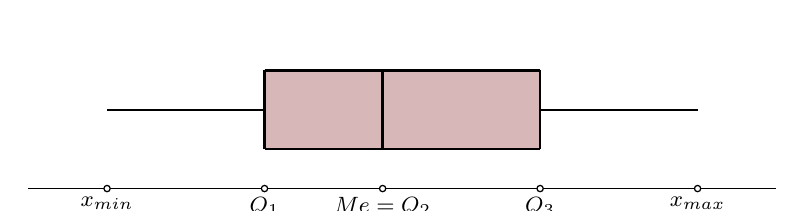
\begin{tikzpicture}
                    % \clip (0,0) rectangle (14.000000,10.000000);
                    {\footnotesize
                    
                    % Marking point x_{min} by circle
                    \draw [line width=0.016cm] (1.500000,1.000000) circle (0.040000);%
                    \draw (1.500000,1.000000) node [anchor=north] { $x_{min}$ };%
                    
                    % Marking point Q_1 by circle
                    \draw [line width=0.016cm] (3.500000,1.000000) circle (0.040000);%
                    \draw (3.500000,1.000000) node [anchor=north] { $Q_1$ };%
                    
                    % Marking point Me=Q_2 by circle
                    \draw [line width=0.016cm] (5.000000,1.000000) circle (0.040000);%
                    \draw (5.000000,1.000000) node [anchor=north] { $Me=Q_2$ };%
                    
                    % Marking point Q_3 by circle
                    \draw [line width=0.016cm] (7.000000,1.000000) circle (0.040000);%
                    \draw (7.000000,1.000000) node [anchor=north] { $Q_3$ };%
                    
                    % Marking point x_{max} by circle
                    \draw [line width=0.016cm] (9.000000,1.000000) circle (0.040000);%
                    \draw (9.000000,1.000000) node [anchor=north] { $x_{max}$ };%
                    
                    % Drawing segment a b
                    \draw [line width=0.016cm] (0.500000,1.000000) -- (1.460000,1.000000);%
                    \draw [line width=0.016cm] (1.540000,1.000000) -- (3.460000,1.000000);%
                    \draw [line width=0.016cm] (3.540000,1.000000) -- (4.960000,1.000000);%
                    \draw [line width=0.016cm] (5.040000,1.000000) -- (6.960000,1.000000);%
                    \draw [line width=0.016cm] (7.040000,1.000000) -- (8.960000,1.000000);%
                    \draw [line width=0.016cm] (9.040000,1.000000) -- (10.000000,1.000000);%
                    
                    % Changing color 215 183 183
                    \definecolor{r215g183b183}{rgb}{0.843137,0.717647,0.717647}%
                    \color{r215g183b183}% 
                    
                    % Filling rectangle left-bottom: f right-top: i
                    \fill (3.500000,2.500000) -- (7.000000,2.500000) -- (7.000000,1.500000) -- (3.500000,1.500000);%
                    
                    % Changing color 0 0 0
                    \definecolor{r0g0b0}{rgb}{0.000000,0.000000,0.000000}%
                    \color{r0g0b0}% 
                    
                    % Drawing segment c d
                    \draw [line width=0.032cm] (1.500000,2.000000) -- (3.500000,2.000000);%
                    
                    % Drawing segment e f
                    \draw [line width=0.032cm] (3.500000,1.500000) -- (3.500000,2.500000);%
                    
                    % Drawing segment g h
                    \draw [line width=0.032cm] (5.000000,1.500000) -- (5.000000,2.500000);%
                    
                    % Drawing segment i j
                    \draw [line width=0.032cm] (7.000000,1.500000) -- (7.000000,2.500000);%
                    
                    % Drawing segment k l
                    \draw [line width=0.032cm] (7.000000,2.000000) -- (9.000000,2.000000);%
                    
                    % Drawing segment e i
                    \draw [line width=0.032cm] (3.500000,1.500000) -- (7.000000,1.500000);%
                    
                    % Drawing segment f j
                    \draw [line width=0.032cm] (3.500000,2.500000) -- (7.000000,2.500000);%
                    \color{black}
                    }
                    \end{tikzpicture}
                \end{figure}
            \end{block}
        \end{frame}


        %%%% naloge

        \begin{frame}
            \only<2->{\begin{exampleblock}{Naloga}
                Izračunajte aritmetično sredino količin.
                \begin{itemize}
                    \item $1.5~s$, $3.5~s$, $1~s$
                    \item $4~km$, $2000~m$, $3~km$
                    \item $4~€$, $2~€$, $3~€$, $1~€$, $5~€$
                \end{itemize}
            \end{exampleblock}}

            \only<3->{\begin{exampleblock}{Naloga}
                Izračunajte aritmetično sredino danim podatkom.
                \begin{itemize}
                    \item $2, 3, 1, 8, 19, 2, 7$
                    \item $13, 39, 12$
                    \item $0.3, 0.4, 0.5, 0.7, 0.6$
                \end{itemize}            \end{exampleblock}}
        \end{frame}

        \begin{frame}
            \only<2->{\begin{exampleblock}{Naloga}
                Določite modus danim številskim podatkom.
                \begin{itemize}
                    \item $1, 4, 2, 4, 1, 6, 3, 4, 1, 4, 6, 4, 4, 8$
                    \item $3, 25, 10, 3, 5, 7, 5, 7, 9, 4, 49$
                    \item $\dfrac{1}{3}, \dfrac{3}{4}, \dfrac{1}{2}, \dfrac{6}{8}, \dfrac{2}{9}$
                    \item $\dfrac{1}{2}, \dfrac{2}{4}, \dfrac{1}{4}, \dfrac{5}{10}, \dfrac{8}{9}$
                \end{itemize}
            \end{exampleblock}}

            \only<3->{\begin{exampleblock}{Naloga}
                V porodnišnici so izmerili dolžine dojenčkov, ki so se rodili v enem dnevu.  \\
                $50, 51, 51, 44, 47, 48, 53, 49, 52, 55, 46, 50, 50, 49, 47, 47$ \\
                Določite mediano podatkov.
            \end{exampleblock}}

        \end{frame}

        \begin{frame}
        
            \only<2->{\begin{exampleblock}{Naloga}
             
             Otroci v vrtcu so metali žogo na koš in si zapisovali dosežke. Podatki so prikazani v preglednici. \\

                 \begin{table}
                     \centering
                     \begin{tabular}{||c|c|c|c|c|c|c|c|c|c||} 
                     \hhline{|t:==========:t|}
                     \rowcolor[rgb]{0.843,0.718,0.718} 
                     Otrok  & Jaka & Jure & Miha & Polona & Valerija & Tina & Mojca & Cene & Darja   \\ 
                     \hhline{|:==========:|}
                     Št.~košev & $5$ & $7$ & $10$ & $8$ & $5$ & $6$ & $9$ & $9$& $4$  \\ 
                     \hhline{|b:==========:b|}
                     \end{tabular}
                 \end{table}

                Izračunajte, koliko košev je otrok zadel v povprečju. Podatke uredite po vrsti in določite $Mo$, $Me$ ter narišite škatlo z brki.

            \end{exampleblock}}

     \end{frame}




    \subsection{Mere razpršenosti}

        \begin{frame}
            \frametitle{Mere razpršenosti}

            \only<2->{\begin{block}{}
                Informacijo o \textbf{porazdelitvi} oziroma \textbf{razpršenosti} podatkov lahko izračunamo s pomočjo: 
                variacijskega razmika, interkvartilnega ranga, variance in standarnega odklona.
            \end{block}}

            \only<3->{\begin{alertblock}{Variacijski razmik}
                \textbf{Variacijski razmik} $R$ je razlika med maksimalno in minimalno vrednostjo statistične spremenljivke:
                $$R=x_{max}-x_{min}.$$
            \end{alertblock}}

            \only<4->{\begin{block}{}
                Variacijski razmik je zelo odvisen od ekstremnih vrednosti, posebno osamelcev, 
                zato ga uporabljamo le v kombinaciji z drugimi merami razpršenosti.
            \end{block}}

        \end{frame}

        \begin{frame}
            \only<2->{\begin{alertblock}{Interkvartilni rang}
                \textbf{Interkvartilni rang} oziroma \textbf{medčetrtinski razmik} $IR$ je razlika med vrednostjo prvega in tretjega kvartila:
                $$IR=Q_3-Q_1.$$
            \end{alertblock}}

            \only<3->{\begin{alertblock}{}
                \textbf{Osamelec} je podatek, katerega vrednost je za več kot $3$-kratnik interkvartilnega ranga~$IR$ nad tretjim kvartilom $Q_3$ ali pod prvim kvartilom $Q_1$. \\
                Podatek je ``pogojno osamelec'', če je njegova vrednost za več kot $1.5$-kratnik interkvartilnega ranga~$IR$ nad tretjim kvartilom $Q_3$ ali pod prvim kvartilom $Q_1$.

            \end{alertblock}}

            \only<4->{\begin{block}{}
                Interkvartilni rang je mera razpršenosti, ki ni občutljiva na osamelce.
            \end{block}}
        \end{frame}

        \begin{frame}

            \only<2->{\begin{alertblock}{Varianca}
                \textbf{Varianca} $\sigma^2$ predstavlja aritmetično sredino kvadratov odmikov vrednosti statistične spremenljivke od aritmetične sredine:
                $$\sigma^2=\dfrac{(x_1-\overline{x})^2+(x_2-\overline{x})^2+\cdots+(x_n-\overline{x})^2}{N}=\dfrac{1}{N}\sum_{i=1}^n(x_i-\overline{x})^2.$$
            \end{alertblock}}

            % \begin{block}{}
            %     Večja kot je varianca, bolj so podatki razpršeni.
            % \end{block}

            \only<3->{\begin{alertblock}{Standardni odklon}
                \textbf{Standardni odklon} $\sigma$ izračunamo kot koren variance:
                $$\sigma=\sqrt{\dfrac{(x_1-\overline{x})^2+(x_2-\overline{x})^2+\cdots+(x_n-\overline{x})^2}{N}}=\sqrt{\dfrac{1}{N}\sum_{i=1}^n(x_i-\overline{x})^2}.$$
                Predstavlja povprečje odmikov vrednosti statistične spremenljivke od aritmetične sredine.
            \end{alertblock}}
        \end{frame}


        %%% naloge

        \begin{frame}
        
            \only<2->{\begin{exampleblock}{Naloga}
             
                V preglednici so predstavljene cene treh izdelkov v trgovini po posameznih mesecih leta 2019. \\
                Izračunajte povprečno ceno in standardni odklon cene vsakega izdelka.

                 \begin{table}
                     \centering
                     \begin{tabular}{||c|c|c|c|c|c|c|c|c|c|c|c||} 
                     \hhline{|t:============:t|}
                     \rowcolor[rgb]{0.843,0.718,0.718} 
                     Izdelek  & Jan & Feb & Mar & Apr & Maj & Jun & Jul & Avg & Sep & Okt & Nov    \\ 
                     \hhline{|:============:|}
                     Kruh  & $3.35$ & $3.29$ & $3.34$ & $3.38$ & $3.38$ & $3.37$ & $3.38$ & $3.55$ & $3.53$ & $3.54$ & $3.49$ \\ 
                     \hhline{|:============:|}
                     Jagode & $8.73$ & $7.18$ & $5.52$ & $4.48$ & $5.72$ & $5.64$ & $6.49$ & $6.58$ & $7.15$ & $7.58$ & $8.34$ \\ 
                     \hhline{|:============:|}
                     Cvetača & $2.04$ & $2.17$ & $1.58$ & $1.75$ & $2.13$ & $1.85$ & $1.93$ & $1.87$ & $1.81$ & $1.99$ & $1.80$ \\ 
                     \hhline{|b:============:b|}
                     \end{tabular}
                 \end{table}
             
                \end{exampleblock}}
 \end{frame}


     \begin{frame}
        
        \only<2->{\begin{exampleblock}{Naloga}
         
            V preglednici je prikazano število rojstev v Sloveniji po letih. \\
            Izračunajte povprečno število rojstev in standardni odklon.

             \begin{table}
                 \centering
                 \begin{tabular}{||c|c|c|c|c|c|c|c|c|c||} 
                 \hhline{|t:==========:t|}
                 \rowcolor[rgb]{0.843,0.718,0.718} 
                 Leto   & $2013$ & $2014$ & $2015$ & $2016$ & $2017$ & $2018$ & $2019$ & $2020$ & $2021$    \\ 
                 \hhline{|:==========:|}
                 Število  & $21111$ & $21165$ & $20641$ & $20345$ & $20241$ & $19585$ & $19328$ & $18767$ & $18989$ \\ 
                 \hhline{|b:==========:b|}
                 \end{tabular}
             \end{table}
        \end{exampleblock}}


             \only<3->{\begin{exampleblock}{Naloga}
         
                Pridobili smo podatke (urejene po velikosti): $1, 13, 14, 15, 15, 15, 17, 18, 18, 19, 19, 19$, $19, 20$ in $40$.
                \begin{itemize}
                    \item Opišite razpršenost podatkov $R$, $IR$, $Q_1$, $Q_3$, $\sigma$, $\overline{x}$.
                    \item Največjo in najmanjšo vrednost (v tem primeru sta to osamelca) odstranimo. Kako se spremeni razpršenost podatkov? 
                \end{itemize}
                
            \end{exampleblock}}
    
         
 \end{frame}



    \subsection{Grafično prikazovanje podatkov}
        
        \begin{frame}
            \frametitle{Grafično prikazovanje podatkov}

            \vskip-1.3em
            \begin{columns}
                \column{0.45\textwidth}
                    \begin{alertblock}{Strukturni krog}
                        \textbf{Strukturni krog} ali \textbf{krožni diagram} uporabljamo, kadar so podatki razvrščeni v malo frekvenčnih razredov 
                        ali ne dosežejo veliko različnih diskretnih vrednosti.
                    \end{alertblock}

                    \begin{block}{}
                        Celoto predstavlja $360^\circ$, za ostale deleže središčne kote izračunamo s sklepnim računom.
                    \end{block}
                \column{0.5\textwidth}            
                \begin{block}{}
                    \begin{figure}[H]
                        \includegraphics[scale=0.25]{../../Slike_in_skice/10921.jpg}
                        \includegraphics[scale=0.25]{../../Slike_in_skice/1092.jpg}
                    \end{figure}
                \end{block}
            \end{columns}

        \end{frame}

        \begin{frame}

            \begin{alertblock}{Stolpčni diagram}
                \textbf{Stolpčni diagram} uporabljamo, ko so podatki razvrščeni v veliko frekvenčnih razredov
                ali lahko dosežejo veliko diskretnih vrednosti.
            \end{alertblock}

            \vskip-1.3em

            \begin{columns}
                \column{0.43\textwidth}

                    \begin{block}{}
                        Stolpčni diagrami so lahko \textbf{pokončni} ali \textbf{ležeči}. 
                        Če želimo prikazati več podatkov naenkrat, uporabimo \textbf{sestavljeni} ali \textbf{strukturni} stolpčni diagram.
                    \end{block}
                \column{0.55\textwidth}            
                \begin{block}{}
                    \begin{figure}[H]
                        \includegraphics[scale=0.28]{../../Slike_in_skice/1093.jpg}
                    \end{figure}
                \end{block}
            \end{columns}
    
        \end{frame}

        \begin{frame}
            \vskip-1.3em

            \begin{columns}
                \column{0.49\textwidth}

            \begin{block}{}
                \begin{figure}[H]
                    \includegraphics[scale=0.19]{../../Slike_in_skice/1095.jpg}
                \end{figure}
            \end{block}

            \column{0.49\textwidth}            
            \begin{block}{}
                \begin{figure}[H]
                    \includegraphics[scale=0.19]{../../Slike_in_skice/1097.jpg} 
                % \end{figure}
            % \end{block}

            % \begin{block}{}
                % \begin{figure}[H]
                    \includegraphics[scale=0.19]{../../Slike_in_skice/1096.jpg}
                \end{figure}
            \end{block}

        \end{columns}

        \end{frame}

        \begin{frame}

                    \begin{alertblock}{Histogram}
                        \textbf{Histogram} uporabljamo za prikaz grupiranih podatkov. 
                    \end{alertblock}

                    \vskip-1.5em
            \begin{columns}
                \column{0.32\textwidth}


                    \begin{block}{}
                        Širine frekvenčnih razredov niso nujno enake.
                        Meje razredov narišemo na vodoravni osi, frekvence posameznih razredov pa na navpični osi.
                    \end{block}
                \column{0.65\textwidth}
                    \begin{block}{}
                        \begin{figure}
                            \includegraphics[scale=0.33]{../../Slike_in_skice/1098.jpg}
                        \end{figure}
                    \end{block}
            \end{columns}


        \end{frame}

        \begin{frame}

            \begin{alertblock}{Linijski diagram}
                \textbf{Linijski diagram/poligon} uporabljamo, ko želimo prikazati postopno spreminjanje vrednosti nekega podatka skozi daljše časovno obdobje.
                Frekvenčne porazdelitve ponazorimo s \textbf{frekvenčnim poligonom}, podatki so lahko zvezni ali grupirani.
            \end{alertblock}

            \vskip-1.3em
            \begin{columns}
                \column{0.58\textwidth}

                    \begin{block}{}
                        \begin{figure}[H]
                            \includegraphics[scale=0.23]{../../Slike_in_skice/1166.jpg}
                        \end{figure}
                    \end{block}

                \column{0.4\textwidth}
                    \begin{block}{}
                        \begin{figure}[H]
                            \includegraphics[scale=0.23]{../../Slike_in_skice/1099.jpg}
                        \end{figure}
                    \end{block}
            \end{columns}

        \end{frame}


        %%%% naloge

        \begin{frame}


            \only<2->{\begin{exampleblock}{Naloga}
         
                Na matematičnem testu je bilo mogoče doseči $50$ točk. Dosežki so bili: 
                $35, 22, 41, 47, 36, 30, 27, 19, 31, 43, 48, 44, 23, 26, 36, 10, 33, 14, 9$. \\
                Razdelite jih v pet enako velikih razredov ter predstavite s histogramom.
                
            \end{exampleblock}}

        
            \only<3->{\begin{exampleblock}{Naloga}
             
             Otroci v vrtcu so metali žogo na koš in si zapisovali dosežke. Podatki so prikazani v preglednici. \\
             Izračunajte, koliko košev je otrok zadel v povprečju. Podatke uredite po vrsti in določite $Mo$, $Me$ ter narišite škatlo z brki.

                 \begin{table}
                     \centering
                     \begin{tabular}{||c|c|c|c|c|c|c|c|c|c||} 
                     \hhline{|t:==========:t|}
                     \rowcolor[rgb]{0.843,0.718,0.718} 
                     Otrok  & Jaka & Jure & Miha & Polona & Valerija & Tina & Mojca & Cene & Darja   \\ 
                     \hhline{|:==========:|}
                     Št.~košev & $5$ & $7$ & $10$ & $8$ & $5$ & $6$ & $9$ & $9$& $4$  \\ 
                     \hhline{|b:==========:b|}
                     \end{tabular}
                 \end{table}
            \end{exampleblock}}

     \end{frame}

     \begin{frame}


   
        \only<2->{\begin{exampleblock}{Naloga}
         
            Bojana beleži, koliko časa potrebuje za pot do šole. Podatke je zapisala v preglednico. \\ 
            S stolpčnim diagramom predstavite, kako pogosto v šolo potuje $8$ minut, $9$ minut ... 

             \begin{table}
                 \centering
                 \begin{tabular}{||c|c|c|c|c|c|c|c|c|c|c||} 
                 \hhline{|t:===========:t|}
                 \rowcolor[rgb]{0.843,0.718,0.718} 
                 Dan  & 1. & 2. & 3. & 4. & 5. & 6. & 7. & 8. & 9. & 10.   \\ 
                 \hhline{|:===========:|}
                 Čas [min] & $9$ & $11$ & $10$ & $8$ & $11$ & $10$ & $9$ & $12$& $9$ & $11$ \\ 
                 \hhline{|b:===========:b|}
                 \end{tabular}
             \end{table}
        \end{exampleblock}}

        \only<3->{\begin{exampleblock}{Naloga}
         
            V domu ostarelih občanov je $500$ oskrbovancev. Od $50$ do $60$ let jih je $15~\%$, med $60$ in $70$ leti je $160$ oskrbovancev,
            med $70$ in $80$ leti pa $200$ starostnikov. Drugi so stari med $80$ in $90$ let.
            \begin{itemize}
                \item Iz grupiranih podatkov izračunajte povprečno starost oskrbovancev tega doma.
                \item Grafično ponazorite starost oskrbovancev.
            \end{itemize}
            
        \end{exampleblock}}


 \end{frame}


% 2. letnik
% \chapter{Geometrija v ravnini}

\section{Osnovni geometrijski pojmi}

            
                Evklid je v prvi knjigi \textit{Elementov} postavil $23$ 'opredelitev' temeljnih geometrijskih pojmov.
                Med njimi so:
                \begin{itemize}
                    \item \textbf{Točka} je tisto, kar nima delov -- nima razsežnosti.
                    \item \textbf{Črta} je dolžina brez širine -- ena razsežnost.
                    \item \textbf{Ploskev} je tisto, kar ima samo dolžino in širino -- dve razsežnosti.
                \end{itemize}
            
                ~
            
                Tem trditvam sledijo \textbf{aksiomi} (temeljne resnice) -- privzamemo jih kot veljavne hipoteze,
                 \textbf{izreki}~-- dokazujemo jih z aksiomi in prej dokazanimi izreki, 
                 in \textbf{definicije} -- opisi novih pojmov in lastnosti.
            
        
                ~
        
            \subsection*{Incidenčni aksiomi}

            \begin{definicija}
                \textit{Incidenca} je relacija, ki povezuje točko in premico -- premica in točka sta v relaciji,
                 če točka leži na premici; $A~R~p$, če $A\in p$.
            \end{definicija}

            \begin{aksiom}
                Za dve različni točki $A$ in $B$ obstaja natanko določena premica $p$, tako da točki $A$ in $B$ ležita na njej.
            \end{aksiom}

            \begin{aksiom}
                Za vsako premico $p$ obstajata vsaj dve različni točki $P$ in $Q$, ki ležita na njej.
            \end{aksiom}

            \begin{aksiom}
                Obstajajo tri različne točke, ki ne ležijo hkrati na isti premici.
            \end{aksiom}
        

            ~
        
            \begin{definicija}
                Točke $A_1, A_2, A_3, \dots$, ki ležijo na isti premici, so \textbf{kolinearne}, 
                če ne ležijo na isti premici, pa so \textbf{nekolinearne}.
            \end{definicija}

            ~

            \begin{izrek}
                Dve različni premici imata lahko največ eno skupno točko.
            \end{izrek}

            \begin{definicija}
                Premici, ki imata natanko eno skupno točko, se \textbf{sekata}, imenujemo ju \textbf{sečnici},
                njuno skupno točko pa \textbf{presečišče} premic.
            \end{definicija}

            \begin{definicija}
                Premici, ki ležita na isti ravnini in nimata nobene skupne točke ali imata vse točke skupne -- sovpadata, sta \textbf{vzporedni}, imenujemo ju \textbf{vzporednici}.
            \end{definicija}
        

            ~
        
            \begin{aksiom}
                Če so tri različne točke kolinearne, ena vedno leži med drugima dvema.

                \begin{figure}[H]
                    \centering
                    \begin{tikzpicture}
                        % \clip (0,0) rectangle (14.000000,10.000000);
                        {\footnotesize

                        % Drawing line A B
                        \draw [line width=0.016cm] (1.000000,1.250000) -- (1.961194,1.490299);%
                        \draw [line width=0.016cm] (2.038806,1.509701) -- (3.461194,1.865299);%
                        \draw [line width=0.016cm] (3.538806,1.884701) -- (3.961194,1.990299);%
                        \draw [line width=0.016cm] (4.038806,2.009701) -- (5.000000,2.250000);%

                        % Marking point A by circle
                        \draw [line width=0.016cm] (2.000000,1.500000) circle (0.040000);%
                        \draw (2.000000,1.500000) node [anchor=south] { $A$ };%

                        % Marking point C by circle
                        \draw [line width=0.016cm] (3.500000,1.875000) circle (0.040000);%
                        \draw (3.500000,1.875000) node [anchor=south] { $C$ };%

                        % Marking point B by circle
                        \draw [line width=0.016cm] (4.000000,2.000000) circle (0.040000);%
                        \draw (4.000000,2.000000) node [anchor=south] { $B$ };%
                        }
                    \end{tikzpicture}
                \end{figure}
            \end{aksiom}

            \begin{aksiom}
                Če sta $A$ in $B$ različni točki premice $p$, potem na premici $p$ ležita vsaj še točki $C$ in $D$,
                in sicer $C$ leži med $A$ in $B$, $D$ pa tako, da je $C$ med $A$ in $D$.

                \begin{figure}[H]
                    \centering
                    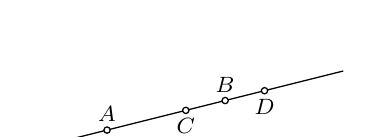
\begin{tikzpicture}
                        % \clip (0,0) rectangle (14.000000,10.000000);
                        {\footnotesize

                        % Drawing line A B
                        \draw [line width=0.016cm] (1.000000,1.250000) -- (1.961194,1.490299);%
                        \draw [line width=0.016cm] (2.038806,1.509701) -- (2.961194,1.740299);%
                        \draw [line width=0.016cm] (3.038806,1.759701) -- (3.461194,1.865299);%
                        \draw [line width=0.016cm] (3.538806,1.884701) -- (3.961194,1.990299);%
                        \draw [line width=0.016cm] (4.038806,2.009701) -- (5.000000,2.250000);%

                        % Marking point A by circle
                        \draw [line width=0.016cm] (2.000000,1.500000) circle (0.040000);%
                        \draw (2.000000,1.500000) node [anchor=south] { $A$ };%

                        % Marking point C by circle
                        \draw [line width=0.016cm] (3.000000,1.750000) circle (0.040000);%
                        \draw (3.000000,1.750000) node [anchor=north] { $C$ };%

                        % Marking point B by circle
                        \draw [line width=0.016cm] (3.500000,1.875000) circle (0.040000);%
                        \draw (3.500000,1.875000) node [anchor=south] { $B$ };%

                        % Marking point D by circle
                        \draw [line width=0.016cm] (4.000000,2.000000) circle (0.040000);%
                        \draw (4.000000,2.000000) node [anchor=north] { $D$ };%
                        }
                    \end{tikzpicture}
                \end{figure}
            \end{aksiom}

            \begin{izrek}
                Med dvema različnima točkama premice je neskončno mnogo točk.
            \end{izrek}

        
            ~

        
            \begin{definicija}
                Množica točk premice, ki ležijo med različnima točkama $A$ in $B$, vključno z $A$ in $B$,
                je \textbf{daljica~$AB$}. Točki $A$ in $B$ sta njeni \textbf{krajišči}.

                \begin{figure}[H]
                    \centering
                    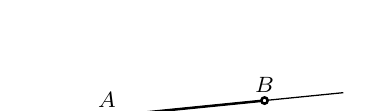
\begin{tikzpicture}
                        % \clip (0,0) rectangle (14.000000,10.000000);
                        {\footnotesize

                        % Drawing line A B
                        \draw [line width=0.016cm] (1.000000,1.400000) -- (1.960199,1.496020);%
                        \draw [line width=0.016cm] (2.039801,1.503980) -- (3.960199,1.696020);%
                        \draw [line width=0.016cm] (4.039801,1.703980) -- (5.000000,1.800000);%

                        % Drawing segment A B
                        \draw [line width=0.032cm] (2.039801,1.503980) -- (3.960199,1.696020);%

                        % Marking point A by circle
                        \draw [line width=0.032cm] (2.000000,1.500000) circle (0.040000);%
                        \draw (2.000000,1.500000) node [anchor=south] { $A$ };%

                        % Marking point B by circle
                        \draw [line width=0.032cm] (4.000000,1.700000) circle (0.040000);%
                        \draw (4.000000,1.700000) node [anchor=south] { $B$ };%
                        }
                    \end{tikzpicture}
                \end{figure}
            \end{definicija}

            \begin{definicija}
                Poljubna točka premice razdeli premico na dva \textbf{poltraka}. To točko imenujemo \textbf{izhodišče}, ponavadi jo označimo z $O$.

                \begin{figure}[H]
                    \centering
                    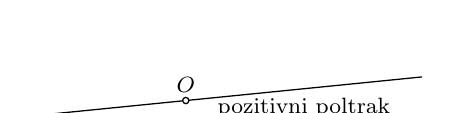
\begin{tikzpicture}
                        % \clip (0,0) rectangle (14.000000,10.000000);
                        {\footnotesize

                        % Drawing line O B
                        \draw [line width=0.016cm] (1.000000,1.300000) -- (2.960199,1.496020);%
                        \draw [line width=0.016cm] (3.039801,1.503980) -- (6.000000,1.800000);%

                        % Marking point O by circle
                        \draw [line width=0.016cm] (3.000000,1.500000) circle (0.040000);%
                        \draw (3.000000,1.500000) node [anchor=south] { $O$ };%

                        % Marking point poz
                        \draw (4.500000,1.400000) node  {pozitivni poltrak };%
                        }
                    \end{tikzpicture}
                \end{figure}
            \end{definicija}

            \begin{definicija}
                Premica, na kateri leži daljica oziroma poltrak, je \textbf{nosilka} daljice oziroma poltraka.
            \end{definicija}
        

            ~
        
            \begin{definicija}
                \textbf{Enostavni lik} je množica točk v ravnini, ki jo omejuje sklenjena krivulja, ki sama sebe ne seka.
            \end{definicija}

            \begin{definicija}

                Množica točk v ravnini je \textbf{konveksna}, če za poljubni točki $A$ in $B$ iz te množice velja, da je daljica $AB$ njena podmnožica.
                
                \begin{multicols}{2}
                $$ \mathcal{M}\text{~konveksna} \Leftrightarrow \forall A, B\in\mathcal{M}\Rightarrow AB\subseteq\mathcal{M} $$
                ~\\~

                \begin{figure}[H]
                    \centering
                    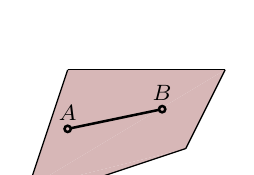
\begin{tikzpicture}
                        % \clip (0,0) rectangle (14.000000,10.000000);
                        {\footnotesize

                        % Changing color 215 183 183
                        \definecolor{r215g183b183}{rgb}{0.843137,0.717647,0.717647}%
                        \color{r215g183b183}% 

                        % Filling triangle C D E
                        \fill (1.500000,1.500000) -- (2.000000,1.500000) -- (3.500000,2.000000);%

                        % Filling triangle C E F
                        \fill (1.500000,1.500000) -- (3.500000,2.000000) -- (4.000000,3.000000);%

                        % Filling triangle C F G
                        \fill (1.500000,1.500000) -- (4.000000,3.000000) -- (2.000000,3.000000);%

                        % Changing color 0 0 0
                        \definecolor{r0g0b0}{rgb}{0.000000,0.000000,0.000000}%
                        \color{r0g0b0}% 

                        % Drawing segment C D
                        \draw [line width=0.016cm] (1.500000,1.500000) -- (2.000000,1.500000);%

                        % Drawing segment D E
                        \draw [line width=0.016cm] (2.000000,1.500000) -- (3.500000,2.000000);%

                        % Drawing segment E F
                        \draw [line width=0.016cm] (3.500000,2.000000) -- (4.000000,3.000000);%

                        % Drawing segment F G
                        \draw [line width=0.016cm] (4.000000,3.000000) -- (2.000000,3.000000);%

                        % Drawing segment G C
                        \draw [line width=0.016cm] (2.000000,3.000000) -- (1.500000,1.500000);%

                        % Marking point A by circle
                        \draw [line width=0.032cm] (2.000000,2.250000) circle (0.040000);%
                        \draw (2.000000,2.250000) node [anchor=south] { $A$ };%

                        % Marking point B by circle
                        \draw [line width=0.032cm] (3.200000,2.500000) circle (0.040000);%
                        \draw (3.200000,2.500000) node [anchor=south] { $B$ };%

                        % Drawing segment A B
                        \draw [line width=0.032cm] (2.039159,2.258158) -- (3.160841,2.491842);%
                        \color{black}
                        }
                    \end{tikzpicture}
                \end{figure}
                
            \end{multicols}

                Množica točk, ki ni konveksna, je \textbf{nekonveksna} oziroma \textbf{konkavna}.
                
            \begin{multicols}{2}
                
                $$ \mathcal{M}\text{~nekonveksna} \Leftrightarrow \exists A, B\in\mathcal{M}\Rightarrow AB\not\subset\mathcal{M} $$
                ~\\~

                \begin{figure}[H]
                    \centering
                    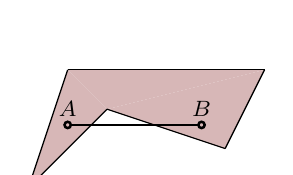
\begin{tikzpicture}
                        % \clip (0,0) rectangle (14.000000,10.000000);
                        {\footnotesize

                        % Changing color 215 183 183
                        \definecolor{r215g183b183}{rgb}{0.843137,0.717647,0.717647}%
                        \color{r215g183b183}% 

                        % Filling triangle C D G
                        \fill (1.500000,1.500000) -- (2.500000,2.500000) -- (2.000000,3.000000);%

                        % Filling triangle D E F
                        \fill (2.500000,2.500000) -- (4.000000,2.000000) -- (4.500000,3.000000);%

                        % Filling triangle D F G
                        \fill (2.500000,2.500000) -- (4.500000,3.000000) -- (2.000000,3.000000);%

                        % Changing color 0 0 0
                        \definecolor{r0g0b0}{rgb}{0.000000,0.000000,0.000000}%
                        \color{r0g0b0}% 

                        % Drawing segment C D
                        \draw [line width=0.016cm] (1.500000,1.500000) -- (2.500000,2.500000);%

                        % Drawing segment D E
                        \draw [line width=0.016cm] (2.500000,2.500000) -- (4.000000,2.000000);%

                        % Drawing segment E F
                        \draw [line width=0.016cm] (4.000000,2.000000) -- (4.500000,3.000000);%

                        % Drawing segment F G
                        \draw [line width=0.016cm] (4.500000,3.000000) -- (2.000000,3.000000);%

                        % Drawing segment G C
                        \draw [line width=0.016cm] (2.000000,3.000000) -- (1.500000,1.500000);%

                        % Marking point A by circle
                        \draw [line width=0.032cm] (2.000000,2.300000) circle (0.040000);%
                        \draw (2.000000,2.300000) node [anchor=south] { $A$ };%

                        % Marking point B by circle
                        \draw [line width=0.032cm] (3.700000,2.300000) circle (0.040000);%
                        \draw (3.700000,2.300000) node [anchor=south] { $B$ };%

                        % Drawing segment A B
                        \draw [line width=0.032cm] (2.040000,2.300000) -- (3.660000,2.300000);%
                        \color{black}
                        }
                    \end{tikzpicture}
                \end{figure}
            \end{multicols}   

        \end{definicija}
        

        ~
        
            \begin{definicija}
                Dva poltraka s skupnim izhodiščem določata dva \textbf{kota}.
                Izhodišče poltrakov imenujemo \textbf{vrh} kota, poltraka pa imenujemo \textbf{kraka} kota.
                
                \begin{figure}[H]
                    \centering
                    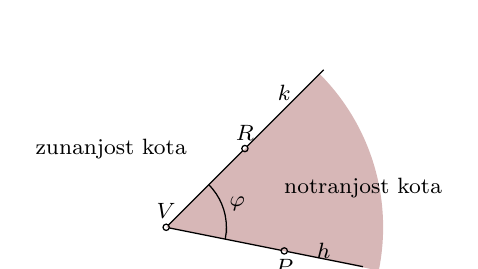
\begin{tikzpicture}
                        % \clip (0,0) rectangle (14.000000,10.000000);
                        {\footnotesize

                        % Changing color 215 183 183
                        \definecolor{r215g183b183}{rgb}{0.843137,0.717647,0.717647}%
                        \color{r215g183b183}% 

                        % Filling circle arc V B 56.31
                        \fill (2.500000,2.500000) -- (5.200000,1.949999) -- (5.204824,1.974235) arc (349:360:2.755449 and 2.755449) --(5.255449,2.500000) arc (0:44:2.755449 and 2.755449) -- (4.455318,4.441451) -- cycle;%

                        % Changing color 0 0 0
                        \definecolor{r0g0b0}{rgb}{0.000000,0.000000,0.000000}%
                        \color{r0g0b0}% 

                        % Drawing line V P
                        % \draw [line width=0.016cm] (1.000000,2.800000) -- (2.460777,2.507845);%
                        \draw [line width=0.016cm] (2.539223,2.492155) -- (3.960777,2.207845);%
                        \draw [line width=0.016cm] (4.039223,2.192155) -- (5.000000,2.000000);%

                        % Drawing line V R
                        % \draw [line width=0.016cm] (1.000000,1.000000) -- (2.471716,2.471716);%
                        \draw [line width=0.016cm] (2.528284,2.528284) -- (3.471716,3.471716);%
                        \draw [line width=0.016cm] (3.528284,3.528284) -- (4.500000,4.500000);%

                        % Marking point V by circle
                        \draw [line width=0.016cm] (2.500000,2.500000) circle (0.040000);%
                        \draw (2.500000,2.500000) node [anchor=south] { $V$ };%

                        % Marking point P by circle
                        \draw [line width=0.016cm] (4.000000,2.200000) circle (0.040000);%
                        \draw (4.000000,2.200000) node [anchor=north] { $P$ };%

                        % Marking point R by circle
                        \draw [line width=0.016cm] (3.500000,3.500000) circle (0.040000);%
                        \draw (3.500000,3.500000) node [anchor=south] { $R$ };%

                        % Marking point h
                        \draw (4.500000,2.000000) node [anchor=south] { $h$ };%

                        % Marking point k
                        \draw (4.000000,4.000000) node [anchor=south] { $k$ };%

                        % Drawing arc V A 56.31
                        \draw [line width=0.016cm] (3.250000,2.350000) -- (3.250800,2.354059) arc (349:360:0.764853 and 0.764853) --(3.264853,2.500000) arc (0:45:0.764853 and 0.764853);%

                        % Marking point \varphi
                        \draw (3.200000,2.800000) node [anchor=west] { $\varphi$ };%

                        % Marking point zun
                        \draw (1.800000,3.500000) node  { zunanjost kota };%

                        % Marking point not
                        \draw (5.000000,3.000000) node  { notranjost kota };%
                        \color{black}
                        }
                    \end{tikzpicture}
                \end{figure}
            \end{definicija}

            
                Če poltraka ne ležita na isti premici, je eden od kotov konveksen, drugi pa je nekonveksen.
            

            
                Kot lahko označimo na več načinov:
                \begin{itemize}
                    \item $\angle(h,k)$, kjer sta $h$ in $k$ poltraka, ki kot določata;
                    \item $\angle PVR$, kjer je $P$ točka na enem poltraku, $V$ vrh kota in $R$ točka na drugem poltraku;
                    \item $\alpha, \beta, \gamma, \dots$ -- z grškimi črkami.
                \end{itemize}
            
        
                ~

        
            \begin{definicija}
                Če poltraka s skupnim izhodiščem ležita na isti premici, vendar na različnih straneh izhodišča,
                določata dva enaka konveksna kota -- \textbf{iztegnjena kota}.

                \begin{figure}[H]
                    \centering
                    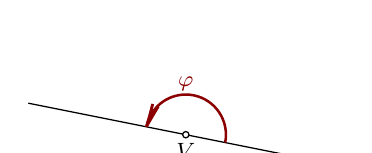
\begin{tikzpicture}
                        % \clip (0,0) rectangle (14.000000,10.000000);
                        {\footnotesize

                        % Drawing line V h
                        \draw [line width=0.016cm] (1.000000,2.000000) -- (2.960777,1.607845);%
                        \draw [line width=0.016cm] (3.039223,1.592155) -- (5.000000,1.200000);%

                        % Marking point V by circle
                        \draw [line width=0.016cm] (3.000000,1.600000) circle (0.040000);%
                        \draw (3.000000,1.600000) node [anchor=north] { $V$ };%

                        % Changing color 139 0 0
                        \definecolor{r139g0b0}{rgb}{0.545098,0.000000,0.000000}%
                        \color{r139g0b0}% 

                        % Drawing arc V h 180.00
                        \draw [line width=0.032cm] (3.500000,1.500000) -- (3.500534,1.502706) arc (349:360:0.509902 and 0.509902) --(3.509902,1.600000) arc (0:168:0.509902 and 0.509902) -- (2.500000,1.700000);%

                        % Marking point \varphi
                        \draw (3.000000,2.050000) node [anchor=south] { $\varphi$ };%

                        % Drawing arrow C A 1.00
                        \draw [line width=0.032cm] (2.651137,1.959148) -- (2.500000,1.700000);%
                        \draw [line width=0.032cm] (2.651137,1.959148) -- (2.538342,1.791430);%
                        \draw [line width=0.032cm] (2.578914,1.989435) -- (2.500000,1.700000);%
                        \draw [line width=0.032cm] (2.578914,1.989435) -- (2.538342,1.791430);%
                        \color{black}
                        }
                    \end{tikzpicture}
                \end{figure}
            \end{definicija}

            \begin{definicija}
                Če se poltraka na isti premici prekrivata, določata \textbf{polni kot} ali \textbf{ničelni kot}.

                \begin{figure}[H]
                    \centering
                    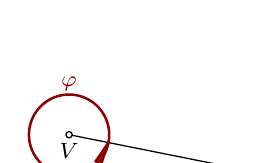
\begin{tikzpicture}
                        % \clip (0,0) rectangle (14.000000,10.000000);
                        {\footnotesize

                        % Drawing line V h
                        % \draw [line width=0.016cm] (1.000000,2.000000) -- (2.960777,1.607845);%
                        \draw [line width=0.016cm] (3.039223,1.592155) -- (5.000000,1.200000);%

                        % Marking point V by circle
                        \draw [line width=0.016cm] (3.000000,1.600000) circle (0.040000);%
                        \draw (3.000000,1.600000) node [anchor=north] { $V$ };%

                        % Changing color 139 0 0
                        \definecolor{r139g0b0}{rgb}{0.545098,0.000000,0.000000}%
                        \color{r139g0b0}% 

                        % Drawing arc V h 360.00
                        \draw [line width=0.032cm] (3.000000,1.600000) circle (0.509902);%

                        % Marking point \varphi
                        \draw (3.000000,2.050000) node [anchor=south] { $\varphi$ };%

                        % Drawing arrow k h 1.00
                        \draw [line width=0.032cm] (3.331960,1.251479) -- (3.500000,1.500000);%
                        \draw [line width=0.032cm] (3.331960,1.251479) -- (3.455661,1.411322);%
                        \draw [line width=0.032cm] (3.402008,1.216456) -- (3.500000,1.500000);%
                        \draw [line width=0.032cm] (3.402008,1.216456) -- (3.455661,1.411322);%
                        \color{black}
                        }
                    \end{tikzpicture} ~~~~~
                    \begin{tikzpicture}
                        % \clip (0,0) rectangle (14.000000,10.000000);
                        {\footnotesize

                        % Drawing line V h
                        % \draw [line width=0.016cm] (1.000000,2.000000) -- (2.960777,1.607845);%
                        \draw [line width=0.016cm] (3.039223,1.592155) -- (5.000000,1.200000);%

                        % Marking point V by circle
                        \draw [line width=0.016cm] (3.000000,1.600000) circle (0.040000);%
                        \draw (3.000000,1.600000) node [anchor=north] { $V$ };%

                        % Changing color 139 0 0
                        \definecolor{r139g0b0}{rgb}{0.545098,0.000000,0.000000}%
                        \color{r139g0b0}% 

                        % Marking point \varphi
                        \draw (3.500000,1.500000) node [anchor=south] { $\varphi$ };%
                        \color{black}
                        }
                    \end{tikzpicture}
                \end{figure}

            \end{definicija}
        
            ~

        
            \begin{definicija}
                Kota s skupnim vrhom, ki imata en skupen krak, presek njunih notranjosti pa je prazen, sta \textbf{sosedna kota}.

                \begin{figure}[H]
                    \centering
                    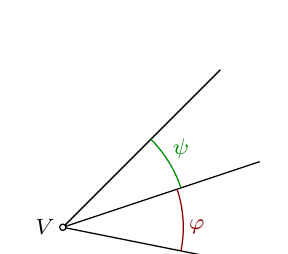
\begin{tikzpicture}
                        % \clip (0,0) rectangle (14.000000,10.000000);
                        {\footnotesize

                        % Drawing line V P
                        \draw [line width=0.016cm] (4.000000,1.000000) -- (1.539223,1.492155);%
                        % \draw [line width=0.016cm] (1.460777,1.507845) -- (1.000000,1.600000);%

                        % Drawing line V Q
                        % \draw [line width=0.016cm] (1.000000,1.333333) -- (1.462053,1.487351);%
                        \draw [line width=0.016cm] (1.537947,1.512649) -- (4.000000,2.333333);%

                        % Drawing line V R
                        % \draw [line width=0.016cm] (1.000000,1.000000) -- (1.471716,1.471716);%
                        \draw [line width=0.016cm] (1.528284,1.528284) -- (3.500000,3.500000);%

                        % Marking point V by circle
                        \draw [line width=0.016cm] (1.500000,1.500000) circle (0.040000);%
                        \draw (1.500000,1.500000) node [anchor=east] { $V$ };%

                        % Changing color 139 0 0
                        \definecolor{r139g0b0}{rgb}{0.545098,0.000000,0.000000}%
                        \color{r139g0b0}% 

                        % Drawing arc V P 29.74
                        \draw [line width=0.016cm] (3.000000,1.200000) -- (3.001601,1.208118) arc (349:360:1.529706 and 1.529706) --(3.029706,1.500000) arc (0:18:1.529706 and 1.529706) -- (2.951206,1.983735);%

                        % Marking point \varphi
                        \draw (3.200000,1.500000) node  { $\varphi$ };%

                        % Changing color 0 139 0
                        \definecolor{r0g139b0}{rgb}{0.000000,0.545098,0.000000}%
                        \color{r0g139b0}% 

                        % Drawing arc V Q 26.57
                        \draw [line width=0.016cm] (3.000000,2.000000) -- (2.994996,2.014768) arc (19:45:1.581139 and 1.581139);%

                        % Marking point \psi
                        \draw (3.000000,2.500000) node  { $\psi$ };%
                        \color{black}
                        }
                    \end{tikzpicture}
                \end{figure}
            \end{definicija}

            \begin{definicija}
                Sosedna kota, katerih kraka, ki  nista skupna, ležita na isti premici, sta \textbf{sokota}.
                
                \begin{figure}[H]
                    \centering
                    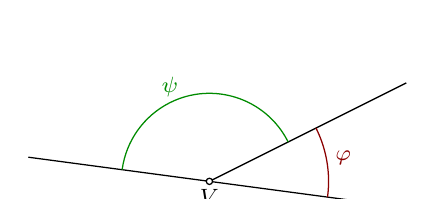
\begin{tikzpicture}
                        % \clip (0,0) rectangle (14.000000,10.000000);
                        {\footnotesize

                        % Drawing line V P
                        \draw [line width=0.016cm] (1.200000,1.806667) -- (3.460351,1.505287);%
                        \draw [line width=0.016cm] (3.539649,1.494713) -- (6.000000,1.166667);%

                        % Drawing line V Q
                        % \draw [line width=0.016cm] (2.700000,1.100000) -- (3.464223,1.482111);%
                        \draw [line width=0.016cm] (3.535777,1.517889) -- (6.000000,2.750000);%

                        % Marking point V by circle
                        \draw [line width=0.016cm] (3.500000,1.500000) circle (0.040000);%
                        \draw (3.500000,1.500000) node [anchor=north] { $V$ };%

                        % Changing color 139 0 0
                        \definecolor{r139g0b0}{rgb}{0.545098,0.000000,0.000000}%
                        \color{r139g0b0}% 

                        % Drawing arc V P 34.16
                        \draw [line width=0.016cm] (5.000000,1.300000) -- (5.001995,1.315578) arc (353:360:1.513275 and 1.513275) --(5.013275,1.500000) arc (0:26:1.513275 and 1.513275) -- (4.853514,2.176757);%

                        % Marking point \varphi
                        \draw (5.200000,1.800000) node  { $\varphi$ };%

                        % Changing color 0 139 0
                        \definecolor{r0g139b0}{rgb}{0.000000,0.545098,0.000000}%
                        \color{r0g139b0}% 

                        % Drawing arc V Q 145.84
                        \draw [line width=0.016cm] (4.500000,2.000000) -- (4.496176,2.007577) arc (27:172:1.118034 and 1.118034) -- (2.391774,1.647764);%

                        % Marking point \psi
                        \draw (3.000000,2.700000) node  { $\psi$ };%
                        \color{black}
                        }
                    \end{tikzpicture}
                \end{figure}
            \end{definicija}

        

            ~\\
        
            \begin{definicija}
                Tri nekolinearne točke $A$, $B$ in $C$ določajo \textbf{trikotnik} $\triangle ABC$.
                Točke $A$, $B$ in $C$ so \textbf{oglišča} trikotnika, daljice $AB$, $BC$ in $AC$ so njegove \textbf{stranice}.

            \begin{figure}[H]
                \centering
                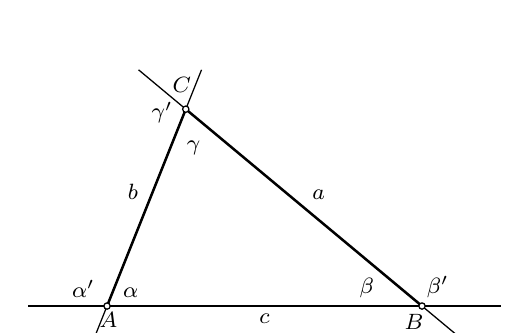
\begin{tikzpicture}
                    % \clip (0,0) rectangle (14.000000,10.000000);
                    {\footnotesize
                    
                    % Marking point A by circle
                    \draw [line width=0.016cm] (2.000000,1.500000) circle (0.040000);%
                    \draw (1.800000,1.530000) node [anchor=north west] { $A$ };%
                    
                    % Marking point B by circle
                    \draw [line width=0.016cm] (6.000000,1.500000) circle (0.040000);%
                    \draw (5.900000,1.500000) node [anchor=north] { $B$ };%
                    
                    % Marking point C by circle
                    \draw [line width=0.016cm] (3.000000,4.000000) circle (0.040000);%
                    \draw (2.950000,4.100000) node [anchor=south] { $C$ };%
                    
                    % Drawing line A B
                    \draw [line width=0.016cm] (1.000000,1.500000) -- (1.960000,1.500000);%
                    \draw [line width=0.016cm] (2.040000,1.500000) -- (5.960000,1.500000);%
                    \draw [line width=0.016cm] (6.040000,1.500000) -- (7.000000,1.500000);%
                    
                    % Drawing line B C
                    \draw [line width=0.016cm] (6.600000,1.000000) -- (6.030729,1.474393);%
                    \draw [line width=0.016cm] (5.969271,1.525607) -- (3.030729,3.974393);%
                    \draw [line width=0.016cm] (2.969271,4.025607) -- (2.400000,4.500000);%
                    
                    % Drawing line A C
                    \draw [line width=0.016cm] (1.800000,1.000000) -- (1.985144,1.462861);%
                    \draw [line width=0.016cm] (2.014856,1.537139) -- (2.985144,3.962861);%
                    \draw [line width=0.016cm] (3.014856,4.037139) -- (3.200000,4.500000);%
                    
                    % Marking point c
                    \draw (4.000000,1.500000) node [anchor=north] { $c$ };%
                    
                    % Marking point a
                    \draw (4.500000,2.750000) node [anchor=south west] { $a$ };%
                    
                    % Marking point b
                    \draw (2.500000,2.750000) node [anchor=south east] { $b$ };%
                    
                    % Marking point \gamma
                    \draw (3.100000,3.700000) node [anchor=north] { $\gamma$ };%
                    
                    % Marking point \gamma'
                    \draw (2.700000,4.200000) node [anchor=north] { $\gamma'$ };%
                    
                    % Marking point \beta
                    \draw (5.300000,1.500000) node [anchor=south] { $\beta$ };%
                    
                    % Marking point \beta'
                    \draw (6.200000,1.500000) node [anchor=south] { $\beta'$ };%
                    
                    % Marking point \alpha
                    \draw (2.300000,1.500000) node [anchor=south] { $\alpha$ };%
                    
                    % Marking point \alpha'
                    \draw (1.700000,1.500000) node [anchor=south] { $\alpha'$ };%
                    
                    % Drawing segment A B
                    \draw [line width=0.032cm] (2.040000,1.500000) -- (5.960000,1.500000);%
                    
                    % Drawing segment B C
                    \draw [line width=0.032cm] (5.969271,1.525607) -- (3.030729,3.974393);%
                    
                    % Drawing segment A C
                    \draw [line width=0.032cm] (2.014856,1.537139) -- (2.985144,3.962861);%
                    }
                \end{tikzpicture}
            \end{figure}

                Koti $\alpha$, $\beta$ in $\gamma$ so \textbf{notranji koti}, 
                njihovi sokoti $\alpha'$, $\beta'$ in $\gamma'$ pa so \textbf{zunanji koti} trikotnika.

            \end{definicija}

            
                Trikotnik je \textbf{pozitivno orientiran}, če si njegova oglišča sledijo v nasprotni smeri vrtenja urnega kazalca; 
                če si sledijo v smeri vrtenja urnega kazalca, pa je \textbf{negativno orientiran}.
            
        
            ~

        
            \begin{definicija}
                Točke $A_1, A_2, A_3, \dots, A_n$ v ravnini, od katerih nobene zaporedne tri niso kolinearne, določajo \textbf{$n$-kotnik}.
                Točke $A_1, A_2, A_3, \dots, A_n$ so \textbf{oglišča} $n$-kotnika;
                daljice, ki povezujejo sosedni oglišči, $A_1A_2, A_2A_3, \dots, A_nA_1$ so \textbf{stranice} $n$-kotnika;
                daljice, ki povezujejo po dve nesosedni oglišči, pa so \textbf{diagonale} $n$-kotnika.
            \end{definicija}

            
                Poljuben $n$-kotnika ima $$\dfrac{n(n-3)}{2}$$ diagonal -- iz vsakega od $n$ oglišč gre $n-3$ diagonal, vsaka pa je šteta dvakrat.
            
            ~
            
                Če za vsako nosilko stranice $n$-kotnika velja, da preostala oglišča ležijo na isti strani te nosilke, je $n$-kotnik \textbf{konveksen}.
            
        




        %%%%% naloge

        ~\\~\\

            \begin{naloga}
                Izračunajte število diagonal: $17$-kotnika, $31$-kotnika in $28$-kotnika.                
            \end{naloga}

            \begin{naloga}
                Ugotovite, ali obstaja $n$-kotnik, ki ima desetino toliko diagonal kot $28$-kotnik.
                Če obstaja, izračunajte, koliko stranic ima.
            \end{naloga}   
            
            \begin{naloga}
                Kateri $n$-kotnik ima štirikrat toliko diagonal kot stranic?
            \end{naloga}
        
            \begin{naloga}
                Izračunajte, kateri $n$-kotnik ima: $104$ diagonale, $230$ diagonal, $2n-5$ diagonal.
            \end{naloga}

            \begin{naloga}
                Pokažite, da ne obstaja $n$-kotnik, ki ima $13$ diagonal.  
            \end{naloga}
            

            \begin{naloga}
                Za vsako od spodnjih izjav ugotovite, ali je pravilna ali nepravilna.
                \begin{itemize}
                    \item Tri različne točke, so vedno nekolinearne.
                    \item Petkotnik ima enako število diagonal in stranic.
                    \item Štiri različne premice se sekajo v največ $4$ različnih točkah.
                    \item Skozi štiri kolinearne točke gredo tri različne premice.
                    \item Vzporedni premici imata lahko neskončno mnogo skupnih točk.
                \end{itemize}
            \end{naloga}

            \begin{naloga}
                Pokažite, da je število diagonal $25$-kotnika večkratnik števila njegovih stranic.
            \end{naloga}

            \begin{naloga}
                Vsota števila stranic in diagonal $n$-kotnika je $105$? Kateri $n$-kotnik je to?
            \end{naloga}
        

            \begin{naloga}
                Izračunajte, kateri $n$-kotnik ima toliko diagonal kot stranic.
            \end{naloga}

            \begin{naloga}
                Člani filatelističnega društva so se domenili, da si bodo za praznike spet pošiljali voščilnice po klasični pošti.
                Ko so se dobili po novem letu, so prinesli vse voščilnice in jih našteli $132$.
                Izračunajte, koliko članov društva, si je medseboj poslalo voščilnice.                
            \end{naloga}


        

\newpage
%%%%%%%%%%%%%%%%%%%%%%%%%%%%%%%%%%%%%%%


\section{Skladnost in merjenje}


    \begin{definicija}
        Dva lika $L$ in $L'$ sta \textbf{skladna}, če lahko lik $L$ prenesemo na lik $L'$ tako,
        da se popolnoma prekrijeta.

        Znak za skladnost je $\cong$.
    \end{definicija}

    
        \textbf{Skladnost} je v množici ravninskih likov \textit{ekvivalenčna relacija}, saj je:
        \begin{itemize}
            \item \textit{refleksivna}: $L\cong L$ -- vsaka množica je skladna sama s seboj;
            \item \textit{simetrična}: $L\cong L' \Rightarrow L'\cong L$ -- če je prva množica skladna z drugo, je tudi druga skladna s prvo;
            \item \textit{tranzitivna}: $L\cong L' \land L'\cong L'' \rightarrow L\cong L''$ -- če je prva množica skladna z drugo in druga skladna s tretjo, 
                    je tudi prva množica skladna s tretjo množico.
        \end{itemize}
    

~


    \begin{definicija}
        Kot, ki je skladen s svojim sokotom, je \textbf{pravi kot}.

        \begin{figure}[H]
            \centering
            \begin{tikzpicture}
            % \clip (0,0) rectangle (14.000000,10.000000);
            {\footnotesize

            % Drawing line V A
            \draw [line width=0.016cm] (1.000000,1.500000) -- (2.960000,1.500000);%
            \draw [line width=0.016cm] (3.040000,1.500000) -- (5.000000,1.500000);%

            % Drawing line V B
            % \draw [line width=0.016cm] (3.000000,1.000000) -- (3.000000,1.460000);%
            \draw [line width=0.016cm] (3.000000,1.540000) -- (3.000000,3.500000);%

            % Marking point V by circle
            \draw [line width=0.016cm] (3.000000,1.500000) circle (0.040000);%

            % Changing color 139 0 0
            \definecolor{r139g0b0}{rgb}{0.545098,0.000000,0.000000}%
            \color{r139g0b0}% 

            % Drawing arc V A 90.00
            \draw [line width=0.032cm] (3.800000,1.500000) arc (360:360:0.800000 and 0.800000) --(3.800000,1.500000) arc (0:90:0.800000 and 0.800000);%

            % Changing color 0 139 0
            \definecolor{r0g139b0}{rgb}{0.000000,0.545098,0.000000}%
            \color{r0g139b0}% 

            % Drawing arc V B 90.00
            \draw [line width=0.032cm] (3.000000,2.200000) arc (90:180:0.700000 and 0.700000);%
            \color{black}
            }
            \end{tikzpicture}

        \end{figure}
        
    \end{definicija}

    
        Če si kraka sledita v nasprotni smeri vrtenja urnega kazalca, je \textbf{orientacija kota pozitivna}, 
        če pa si sledita v smeri vrtenja urnega kazalca, pa je \textbf{orientacija kota negativna}.

        \begin{figure}[H]
                \centering
            \begin{tikzpicture}
            % \clip (0,0) rectangle (14.000000,10.000000);
            {\footnotesize

            % Drawing segment A b
            \draw [line width=0.016cm] (1.500000,1.500000) -- (4.500000,1.500000);%

            % Drawing segment A C
            \draw [line width=0.016cm] (1.500000,1.500000) -- (4.500000,2.785714);%

            % Changing color 139 0 0
            \definecolor{r139g0b0}{rgb}{0.545098,0.000000,0.000000}%
            \color{r139g0b0}% 

            % Drawing arc A B 23.20
            \draw [line width=0.032cm] (3.000000,1.500000) arc (360:360:1.500000 and 1.500000) --(3.000000,1.500000) arc (0:23:1.500000 and 1.500000) -- (2.878718,2.090879);%

            % Drawing arrow Bb U 1.00
            \draw [line width=0.032cm] (2.923918,1.794304) -- (2.878718,2.090879);%
            \draw [line width=0.032cm] (2.923918,1.794304) -- (2.906321,1.995655);%
            \draw [line width=0.032cm] (2.999137,1.816108) -- (2.878718,2.090879);%
            \draw [line width=0.032cm] (2.999137,1.816108) -- (2.906321,1.995655);%

            % Marking point +
            \draw (2.600000,1.700000) node  { $+$ };%
            \color{black}
            }
            \end{tikzpicture} ~~~~~
            \begin{tikzpicture}
            % \clip (0,0) rectangle (14.000000,10.000000);
            {\footnotesize

            % Drawing segment A b
            \draw [line width=0.016cm] (1.500000,1.500000) -- (4.500000,1.500000);%

            % Drawing segment A C
            \draw [line width=0.016cm] (1.500000,1.500000) -- (4.500000,2.785714);%

            % Changing color 139 0 0
            \definecolor{r139g0b0}{rgb}{0.545098,0.000000,0.000000}%
            \color{r139g0b0}% 

            % Drawing arc A B 23.20
            \draw [line width=0.032cm] (3.000000,1.500000) arc (360:360:1.500000 and 1.500000) --(3.000000,1.500000) arc (0:23:1.500000 and 1.500000) -- (2.878718,2.090879);%

            % Drawing arrow Bb B 1.00
            \draw [line width=0.032cm] (3.001963,1.799994) -- (3.000000,1.500000);%
            \draw [line width=0.032cm] (3.001963,1.799994) -- (2.987703,1.598379);%
            \draw [line width=0.032cm] (2.924252,1.790280) -- (3.000000,1.500000);%
            \draw [line width=0.032cm] (2.924252,1.790280) -- (2.987703,1.598379);%

            % Marking point -
            \draw (2.600000,1.700000) node  { $-$ };%
            \color{black}
            }
            \end{tikzpicture}
        \end{figure}
    




        ~

    
        Daljici $AB$ in $CD$, ki nista skladni, lahko premaknemo na poljubni premici tako,
        da levi krajišči sovpadata in da eno od desnih krajišč, npr. $D$ leži med $A$ in $B$.
        V tem primeru je daljica $AB$ \textbf{daljša} od daljice $CD$ oziroma je daljica $CD$ \textbf{krajša} od daljice $AB$.
    

    \begin{aksiom}[Arhimedov aksiom]
        Obstaja tako naravno število $n$, pri katerem je vsota $n$ krajših daljic $CD$ daljša od daljice $AB$,
        vsota $n-1$ krajših daljic $CD$ pa je kvečjemu skladna z daljico $AB$.
        $$n\cdot |CD|>|AB| \quad \quad (n-1)\cdot |CD|\leq |AB|$$

        \begin{figure}[H]
            \centering
            \begin{tikzpicture}
            % \clip (0,0) rectangle (14.000000,10.000000);
            {\footnotesize

            % Drawing line A B
            \draw [line width=0.016cm] (1.000000,1.500000) -- (1.460000,1.500000);%
            \draw [line width=0.016cm] (1.540000,1.500000) -- (2.460000,1.500000);%
            \draw [line width=0.016cm] (2.540000,1.500000) -- (3.460000,1.500000);%
            \draw [line width=0.016cm] (3.540000,1.500000) -- (4.460000,1.500000);%
            \draw [line width=0.016cm] (4.540000,1.500000) -- (5.460000,1.500000);%
            \draw [line width=0.016cm] (5.540000,1.500000) -- (6.460000,1.500000);%
            \draw [line width=0.016cm] (6.540000,1.500000) -- (7.160000,1.500000);%
            \draw [line width=0.016cm] (7.240000,1.500000) -- (7.460000,1.500000);%
            \draw [line width=0.016cm] (7.540000,1.500000) -- (8.100000,1.500000);%

            % Marking point A by circle
            \draw [line width=0.016cm] (1.500000,1.500000) circle (0.040000);%
            \draw (1.500000,1.500000) node [anchor=south] { $A$ };%

            % Marking point B by circle
            \draw [line width=0.016cm] (7.200000,1.500000) circle (0.040000);%
            \draw (7.200000,1.500000) node [anchor=south] { $B$ };%

            % Marking point C by circle
            \draw [line width=0.016cm] (1.500000,1.500000) circle (0.040000);%
            \draw (1.500000,1.500000) node [anchor=north] { $C$ };%

            % Marking point D by circle
            \draw [line width=0.016cm] (2.500000,1.500000) circle (0.040000);%
            \draw (2.500000,1.500000) node [anchor=north] { $D$ };%

            % Marking point E by circle
            \draw [line width=0.016cm] (3.500000,1.500000) circle (0.040000);%

            % Marking point F by circle
            \draw [line width=0.016cm] (4.500000,1.500000) circle (0.040000);%

            % Marking point G by circle
            \draw [line width=0.016cm] (5.500000,1.500000) circle (0.040000);%

            % Marking point H by circle
            \draw [line width=0.016cm] (6.500000,1.500000) circle (0.040000);%

            % Marking point I by circle
            \draw [line width=0.016cm] (7.500000,1.500000) circle (0.040000);%
            }
            \end{tikzpicture}
        \end{figure}
    \end{aksiom}

    % 
        Daljico $CD$, s katero smo izmerili daljico $AB$, imenujemo \textbf{enotska daljica}.
        Tako smo daljici $AB$ priredili natančno določeno število -- \textbf{dolžino} daljice $AB$ oziroma \textbf{razdaljo} točk $A$ in $B$.
        $$ |AB|=d(A,B)$$
    % 
    
        % Daljico $CD$ imenujemo \textbf{enotska daljica}.
        % Daljici $AB$ smo priredili natančno določeno število -- \textbf{dolžino} daljice $AB$ oziroma \textbf{razdaljo} točk $A$ in $B$.

        % $$ |AB|=d(A,B)$$
    





    \begin{aksiom}
        Če je $AB$ poljubna daljica, $A'$ pa točka na poljubnem poltraku, obstaja na tem poltraku natančno določena točka $B'$,
        da je daljica $A'B'$ skladna z daljico $AB$.

        $$A'B'\cong AB$$
    \end{aksiom}

    \begin{izrek}
        Skladni daljici imata enako dolžino.
        % $$|A'B'|=|AB|$$
    \end{izrek}

    ~ 

    \begin{aksiom}
        Naj daljici $AB$ in $BC$ ležita na isti premici in naj imata skupno le točko $B$.
        Daljici $A'B'$ in $B'C'$ naj ležita na tej ali neki drugi premici in naj imata skupno točko $B'$.
        Če velja $AB\cong A'B'$ in $BC\cong B'C'$, potem velja tudi $AC\cong A'C'$.
    \end{aksiom}

    \begin{izrek}
        Dolžina vsote daljic je enaka vsoti dolžin posameznih daljic.
    \end{izrek}




    \subsection*{Enote}


    
        Osnovna enota za merjenje dolžine je \textbf{meter}.

        Iz nje izpeljane enote pa so \textit{decimeter}, \textit{centimeter}, \textit{milimeter}, \textit{kilometer} itd.
        $$ 1~m=10~dm=100~cm=1000~mm$$  $$1~km=1000~m$$ 
    

    
        Enota za merjenje kotov je \textbf{kotna stopinja} -- velikost $\dfrac{1}{360}$ polnega kota.
        
        Izpeljani enoti sta \textit{(kotna) minuta} in \textit{(kotna) sekunda}.
        $$1^\circ=60'=3600''$$ 
    

    
        Velikost kota nič je $0^\circ$, pravega kota je $90^\circ$, iztegnjenega kota je $180^\circ$, polnega kota pa je $360^\circ$.
    

~


    \begin{definicija}
        Kota $\varphi$ in $\psi$, katerih vsota meri $180^\circ$, sta \textbf{suplementarna kota}.

        \begin{figure}[H]
            \centering
            \begin{tikzpicture}
            % \clip (0,0) rectangle (14.000000,10.000000);
            {\footnotesize

            % Drawing line V P
            \draw [line width=0.016cm] (1.200000,1.500000) -- (3.460000,1.500000);%
            \draw [line width=0.016cm] (3.540000,1.500000) -- (6.000000,1.500000);%

            % Drawing line V Q
            % \draw [line width=0.016cm] (3.100000,1.100000) -- (3.471716,1.471716);%
            \draw [line width=0.016cm] (3.528284,1.528284) -- (5.000000,3.000000);%

            % Marking point V by circle
            \draw [line width=0.016cm] (3.500000,1.500000) circle (0.040000);%

            % Changing color 139 0 0
            \definecolor{r139g0b0}{rgb}{0.545098,0.000000,0.000000}%
            \color{r139g0b0}% 

            % Drawing arc V P 45.00
            \draw [line width=0.016cm] (5.000000,1.500000) arc (360:360:1.500000 and 1.500000) --(5.000000,1.500000) arc (0:45:1.500000 and 1.500000);%

            % Marking point \varphi
            \draw (5.200000,1.80000) node  { $\varphi$ };%

            % Changing color 0 139 0
            \definecolor{r0g139b0}{rgb}{0.000000,0.545098,0.000000}%
            \color{r0g139b0}% 

            % Drawing arc V Q 135.00
            \draw [line width=0.016cm] (4.500000,2.500000) arc (45:180:1.414214 and 1.414214);%

            % Marking point \psi
            \draw (3.000000,2.650000) node  { $\psi$ };%
            \color{black}
            }
            \end{tikzpicture}
        \end{figure}
    \end{definicija}

                
    \begin{definicija}
        Kota $\varphi$ in $\psi$, katerih vsota meri $90^\circ$, sta \textbf{komplementarna kota}.

        \begin{figure}[H]
            \centering
            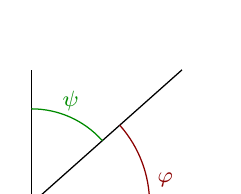
\begin{tikzpicture}
            % \clip (0,0) rectangle (14.000000,10.000000);
            {\footnotesize

            % Drawing line V P
            % \draw [line width=0.016cm] (2.800000,1.500000) -- (3.460000,1.500000);%
            \draw [line width=0.016cm] (3.540000,1.500000) -- (5.800000,1.500000);%

            % Drawing line V Q
            % \draw [line width=0.016cm] (3.050000,1.100000) -- (3.470104,1.473425);%
            \draw [line width=0.016cm] (3.529896,1.526575) -- (5.412500,3.200000);%

            % Drawing line V R
            % \draw [line width=0.016cm] (3.500000,1.100000) -- (3.500000,1.460000);%
            \draw [line width=0.016cm] (3.500000,1.540000) -- (3.500000,3.200000);%

            % Marking point V by circle
            \draw [line width=0.016cm] (3.500000,1.500000) circle (0.040000);%

            % Changing color 139 0 0
            \definecolor{r139g0b0}{rgb}{0.545098,0.000000,0.000000}%
            \color{r139g0b0}% 

            % Drawing arc V P 41.63
            \draw [line width=0.016cm] (5.000000,1.500000) arc (360:360:1.500000 and 1.500000) --(5.000000,1.500000) arc (0:41:1.500000 and 1.500000) -- (4.621114,2.496546);%

            % Marking point \varphi
            \draw (5.200000,1.800000) node  { $\varphi$ };%

            % Changing color 0 139 0
            \definecolor{r0g139b0}{rgb}{0.000000,0.545098,0.000000}%
            \color{r0g139b0}% 

            % Drawing arc V Q 48.37
            \draw [line width=0.016cm] (4.400000,2.300000) -- (4.394865,2.305740) arc (42:90:1.204159 and 1.204159);%

            % Marking point \psi
            \draw (4.000000,2.800000) node  { $\psi$ };%
            \color{black}
            }
            \end{tikzpicture}
        \end{figure}
    \end{definicija}

    
        Sokota sta vedno suplementarna kota.
    




    \subsection*{Skladnost trikotnikov}


    \begin{definicija}
        Dva trikotnika sta \textbf{skladna}, če imata paroma skladne vse stranice in tem stranicam nasprotne kote.
    \end{definicija}

    \begin{aksiom}
        Dva trikotnika sta skladna, če se ujemata v dveh stranicah in v vmesnem kotu.
    \end{aksiom}

    \begin{izrek}
        Trikotnika $\triangle ABC$ in $\triangle A'B'C'$ sta skladna, če se ujemata:
        \begin{enumerate}
            \item v vseh treh stranicah;
            \item v eni stranici in obeh priležnih kotih;
            \item v dveh stranicah in kotu, ki leži nasproti daljši od obeh stranic.
        \end{enumerate}
    \end{izrek}




%%%% naloge


~\\~~\\~\\


    \begin{naloga}
        Izračunajte dolžino daljice, če ena polovica meri $2x-7$ enot, druga polovica pa $x+8$ enot.
    \end{naloga}

    \begin{naloga}
        Izračunaj dolžino $x$ daljice $AB$, če je točka $S$ njeno razpolovišče, točka $R$ pa razpolovišče daljice $SB$ in je $\lvert SR \rvert = \dfrac{x}{3}-1$.
    \end{naloga}

    \begin{naloga}
        Izračunajte velikosti kotov $\angle AVM$ in $\angle FVE$, če poltrak $VM$ obakrat razpolavlja kot.

        \begin{figure}[H]
            \centering
            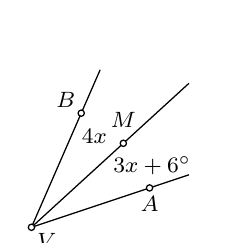
\begin{tikzpicture}
                % \clip (0,0) rectangle (14.000000,10.000000);
                {\footnotesize

                % Marking point V by circle
                \draw [line width=0.016cm] (1.500000,1.500000) circle (0.040000);%
                \draw (1.470000,1.530000) node [anchor=north west] { $V$ };%

                % Marking point A by circle
                \draw [line width=0.016cm] (3.000000,2.000000) circle (0.040000);%
                \draw (3.000000,2.000000) node [anchor=north] { $A$ };%

                % Drawing line V A
                % \draw [line width=0.016cm] (1.200000,1.400000) -- (1.462053,1.487351);%
                \draw [line width=0.016cm] (1.537947,1.512649) -- (2.962053,1.987351);%
                \draw [line width=0.016cm] (3.037947,2.012649) -- (3.500000,2.166667);%

                % Marking point M by circle
                \draw [line width=0.016cm] (2.666950,2.566878) circle (0.040000);%
                \draw (2.666950,2.666878) node [anchor=south] { $M$ };%

                % Marking point B by circle
                \draw [line width=0.016cm] (2.132124,2.949283) circle (0.040000);%
                \draw (2.162124,2.919283) node [anchor=south east] { $B$ };%

                % Drawing line V B
                % \draw [line width=0.016cm] (1.369151,1.200000) -- (1.484008,1.463336);%
                \draw [line width=0.016cm] (1.515992,1.536664) -- (2.116132,2.912618);%
                \draw [line width=0.016cm] (2.148115,2.985947) -- (2.372326,3.500000);%

                % Drawing line V M
                % \draw [line width=0.016cm] (1.200000,1.225727) -- (1.470478,1.473010);%
                \draw [line width=0.016cm] (1.529522,1.526990) -- (2.637428,2.539888);%
                \draw [line width=0.016cm] (2.696472,2.593868) -- (3.500000,3.328489);%

                % Marking point {3x+6^\circ}
                \draw (3.033475,2.283439) node  { ${3x+6^\circ}$ };%

                % Marking point {4x}
                \draw (2.299537,2.658080) node  { ${4x}$ };%
                }
            \end{tikzpicture} ~
            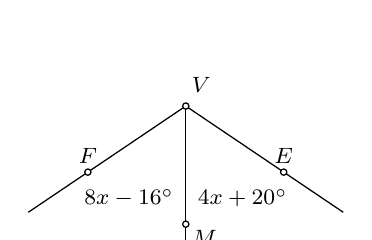
\begin{tikzpicture}
                % \clip (0,0) rectangle (14.000000,10.000000);
                {\footnotesize

                % Marking point V by circle
                \draw [line width=0.016cm] (4.000000,4.000000) circle (0.040000);%
                \draw (3.970000,4.070000) node [anchor=south west] { $V$ };%

                % Marking point M by circle
                \draw [line width=0.016cm] (4.000000,2.500000) circle (0.040000);%
                \draw (3.970000,2.530000) node [anchor=north west] { $M$ };%

                % Drawing line V M
                \draw [line width=0.016cm] (4.000000,2.200000) -- (4.000000,2.460000);%
                \draw [line width=0.016cm] (4.000000,2.540000) -- (4.000000,3.960000);%
                % \draw [line width=0.016cm] (4.000000,4.040000) -- (4.000000,4.200000);%

                % Marking point F by circle
                \draw [line width=0.016cm] (2.756444,3.161211) circle (0.040000);%
                \draw (2.756444,3.161211) node [anchor=south] { $F$ };%

                % Marking point E by circle
                \draw [line width=0.016cm] (5.243556,3.161211) circle (0.040000);%
                \draw (5.243556,3.161211) node [anchor=south] { $E$ };%

                % Drawing line V E
                % \draw [line width=0.016cm] (3.703488,4.200000) -- (3.966838,4.022368);%
                \draw [line width=0.016cm] (4.033162,3.977632) -- (5.210395,3.183578);%
                \draw [line width=0.016cm] (5.276718,3.138843) -- (6.000000,2.650983);%

                % Drawing line V F
                % \draw [line width=0.016cm] (4.296512,4.200000) -- (4.033162,4.022368);%
                \draw [line width=0.016cm] (3.966838,3.977632) -- (2.789605,3.183578);%
                \draw [line width=0.016cm] (2.723282,3.138843) -- (2.000000,2.650983);%

                % Marking point {8x-16^\circ}
                \draw (3.278222,2.830605) node  { ${8x-16^\circ}$ };%

                % Marking point {4x+20^\circ}
                \draw (4.721778,2.830605) node  { ${4x+20^\circ}$ };%
                }
            \end{tikzpicture}


        \end{figure}
    \end{naloga}


    \begin{multicols}{2}
    \begin{naloga}
        Izračunajte velikosti kotov $\alpha$ in $\beta$, če je $\alpha=\beta$.
        Podatke razberite s skice.

        \begin{figure}[H]
            \centering
            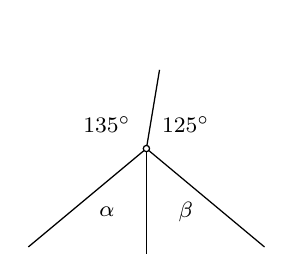
\begin{tikzpicture}
                % \clip (0,0) rectangle (14.000000,10.000000);
                {\footnotesize

                % Marking point A by circle
                \draw [line width=0.016cm] (3.000000,3.000000) circle (0.040000);%

                % Drawing segment A B
                \draw [line width=0.016cm] (3.000000,1.500000) -- (3.000000,2.960000);%

                % Drawing segment A C
                \draw [line width=0.016cm] (3.030729,2.974393) -- (4.500000,1.750000);%

                % Drawing segment A D
                \draw [line width=0.016cm] (2.969271,2.974393) -- (1.500000,1.750000);%

                % Drawing segment A E
                \draw [line width=0.016cm] (3.006576,3.039456) -- (3.166667,4.000000);%

                % Marking point \beta
                \draw (3.500000,2.200000) node  { $\beta$ };%

                % Marking point \alpha
                \draw (2.500000,2.200000) node  { $\alpha$ };%

                % Marking point {125^\circ}
                \draw (3.500000,3.300000) node  { ${125^\circ}$ };%

                % Marking point {135^\circ}
                \draw (2.500000,3.300000) node  { ${135^\circ}$ };%
                }
            \end{tikzpicture}

        \end{figure}
    \end{naloga}




    \begin{naloga}
        Iz podatkov na skici izračunajte neznano velikost kota $x$.

        \begin{figure}[H]
            \centering
            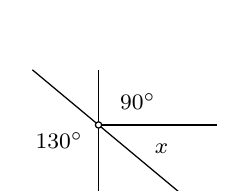
\begin{tikzpicture}
                % \clip (0,0) rectangle (14.000000,10.000000);
                {\footnotesize

                % Marking point A by circle
                \draw [line width=0.016cm] (3.000000,3.000000) circle (0.040000);%

                % Drawing line A B
                \draw [line width=0.016cm] (3.000000,2.000000) -- (3.000000,2.960000);%
                \draw [line width=0.016cm] (3.000000,3.040000) -- (3.000000,3.700000);%

                % Drawing line A C
                \draw [line width=0.016cm] (4.200000,2.000000) -- (3.030729,2.974393);%
                \draw [line width=0.016cm] (2.969271,3.025607) -- (2.160000,3.700000);%

                % Drawing segment A E
                \draw [line width=0.016cm] (3.040000,3.000000) -- (4.500000,3.000000);%

                % Marking point x
                \draw (3.800000,2.700000) node  { $x$ };%

                % Marking point {90^\circ}
                \draw (3.500000,3.300000) node  { ${90^\circ}$ };%

                % Marking point {130^\circ}
                \draw (2.500000,2.800000) node  { ${130^\circ}$ };%
                }
            \end{tikzpicture}

        \end{figure}
    \end{naloga}

\end{multicols}





    \begin{multicols}{2}
        
    \begin{naloga}
        Izračunajte velikost kota $\angle PVQ$, če je $\angle PVR=94^\circ$.

        \begin{figure}[H]
            \centering
            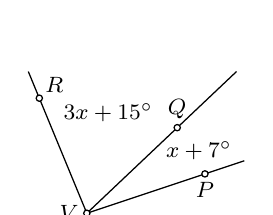
\begin{tikzpicture}
                % \clip (0,0) rectangle (14.000000,10.000000);
                {\footnotesize

                % Marking point V by circle
                \draw [line width=0.016cm] (3.500000,1.500000) circle (0.040000);%
                \draw (3.500000,1.500000) node [anchor=east] { $V$ };%

                % Marking point P by circle
                \draw [line width=0.016cm] (5.000000,2.000000) circle (0.040000);%
                \draw (5.000000,2.000000) node [anchor=north] { $P$ };%

                % Drawing line V P
                % \draw [line width=0.016cm] (2.600000,1.200000) -- (3.462053,1.487351);%
                \draw [line width=0.016cm] (3.537947,1.512649) -- (4.962053,1.987351);%
                \draw [line width=0.016cm] (5.037947,2.012649) -- (5.500000,2.166667);%

                % Marking point Q by circle
                \draw [line width=0.016cm] (4.648153,2.587081) circle (0.040000);%
                \draw (4.648153,2.587081) node [anchor=south] { $Q$ };%

                % Marking point R by circle
                \draw [line width=0.016cm] (2.896583,2.961468) circle (0.040000);%
                \draw (2.866583,2.931468) node [anchor=south west] { $R$ };%

                % Drawing line V R
                % \draw [line width=0.016cm] (3.623865,1.200000) -- (3.515265,1.463027);%
                \draw [line width=0.016cm] (3.484735,1.536973) -- (2.911849,2.924495);%
                \draw [line width=0.016cm] (2.881318,2.998440) -- (2.756809,3.300000);%

                % Drawing line V Q
                % \draw [line width=0.016cm] (3.183146,1.200000) -- (3.470954,1.472499);%
                \draw [line width=0.016cm] (3.529046,1.527501) -- (4.619106,2.559580);%
                \draw [line width=0.016cm] (4.677199,2.614582) -- (5.401122,3.300000);%

                % Marking point {x+7^\circ}
                \draw (4.924076,2.293541) node  { ${x+7^\circ}$ };%

                % Marking point {3x+15^\circ}
                \draw (3.772368,2.774275) node  { ${3x+15^\circ}$ };%
                }
            \end{tikzpicture}

        \end{figure}
    \end{naloga}


    \begin{naloga}
        Izračunajte velikost kota $\angle SVR$, če je $\angle QVS=50^\circ$.

        \begin{figure}[H]
            \centering
            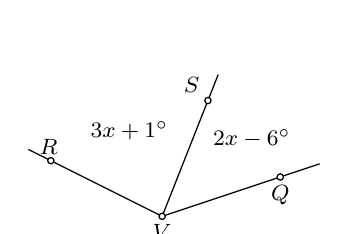
\begin{tikzpicture}
                % \clip (0,0) rectangle (14.000000,10.000000);
                {\footnotesize

                % Marking point V by circle
                \draw [line width=0.016cm] (3.500000,1.500000) circle (0.040000);%
                \draw (3.500000,1.500000) node [anchor=north] { $V$ };%

                % Marking point P by circle
                \draw [line width=0.016cm] (5.000000,2.000000) circle (0.040000);%
                \draw (5.000000,2.000000) node [anchor=north] { $Q$ };%

                % Drawing line V P
                % \draw [line width=0.016cm] (2.600000,1.200000) -- (3.462053,1.487351);%
                \draw [line width=0.016cm] (3.537947,1.512649) -- (4.962053,1.987351);%
                \draw [line width=0.016cm] (5.037947,2.012649) -- (5.500000,2.166667);%

                % Marking point S by circle
                \draw [line width=0.016cm] (4.081159,2.970460) circle (0.040000);%
                \draw (4.081159,2.970460) node [anchor=south east] { $S$ };%

                % Marking point R by circle
                \draw [line width=0.016cm] (2.085787,2.207107) circle (0.040000);%
                \draw (2.055787,2.177107) node [anchor=south] { $R$ };%

                % Drawing line V R
                % \draw [line width=0.016cm] (4.100000,1.200000) -- (3.535777,1.482111);%
                \draw [line width=0.016cm] (3.464223,1.517889) -- (2.121564,2.189218);%
                \draw [line width=0.016cm] (2.050009,2.224995) -- (1.800000,2.350000);%

                % Drawing line V S
                % \draw [line width=0.016cm] (3.381433,1.200000) -- (3.485298,1.462800);%
                \draw [line width=0.016cm] (3.514702,1.537200) -- (4.066457,2.933260);%
                \draw [line width=0.016cm] (4.095862,3.007660) -- (4.211401,3.300000);%

                % Marking point {2x-6^\circ}
                \draw (4.640580,2.485230) node  { ${2x-6^\circ}$ };%

                % Marking point {3x+1^\circ}
                \draw (3.083473,2.588784) node  { ${3x+1^\circ}$ };%
                }
            \end{tikzpicture}

        \end{figure}
    \end{naloga}


    \end{multicols}

        


    \begin{naloga}
        Kot $\varphi=76^\circ 36'53''$ zapišite v stopinjah na štiri mesta natančno, 
        kot $\psi=34.78^\circ$ pa zapišite v stopinjah, minutah in sekundah.
    \end{naloga}

    \begin{naloga}
        Kotu $\varphi=37^\circ 16'43''$ izračunajte suplementarni in komplementarni kot.
    \end{naloga}

    \begin{naloga}
        Razika dveh komplementarnih kotov je $37^\circ 16'$. Izračunajte velikosti kotov.
    \end{naloga}

    \begin{naloga}
        Izračunajte velikost kota $\varphi$, ki je petkratnik svojega komplementarnega kota.
    \end{naloga}





    \begin{naloga}
        Za vsako od spodnjih izjav ugotovite, ali je pravilna ali nepravilna.
        \begin{itemize}
            \item Sokota sta suplementarna.
            % \item Kota z vzporednimi kraki sta skladna.
            \item Kot z velikostjo $45^\circ$ je komplementaren samemu sebi.
            \item Dve premici, ki se sekata, lahko določata kota z velikostjo $43^\circ$ in $137^\circ$.
            \item Vsota velikosti dveh komplementarnih kotov je pravi kot.
            \item Suplementarna kota sta  vedno tudi sokota.
        \end{itemize}
    \end{naloga}

    \begin{naloga}
        Poltrak $VD$ razpolavlja $\angle CVE$, $\angle BVC$ je pravi kot.
        Določite velikosti kotov $\angle AVD$ in $\angle BVE$.

        \begin{figure}[H]
            \centering
            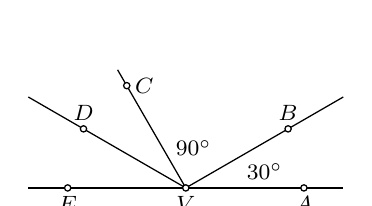
\begin{tikzpicture}
                % \clip (0,0) rectangle (14.000000,10.000000);
                {\footnotesize

                % Marking point V by circle
                \draw [line width=0.016cm] (4.000000,1.500000) circle (0.040000);%
                \draw (4.000000,1.500000) node [anchor=north] { $V$ };%

                % Marking point A by circle
                \draw [line width=0.016cm] (5.500000,1.500000) circle (0.040000);%
                \draw (5.500000,1.500000) node [anchor=north] { $A$ };%

                % Marking point E by circle
                \draw [line width=0.016cm] (2.500000,1.500000) circle (0.040000);%
                \draw (2.500000,1.500000) node [anchor=north] { $E$ };%

                % Drawing line A E
                \draw [line width=0.016cm] (2.000000,1.500000) -- (2.460000,1.500000);%
                \draw [line width=0.016cm] (2.540000,1.500000) -- (3.960000,1.500000);%
                \draw [line width=0.016cm] (4.040000,1.500000) -- (5.460000,1.500000);%
                \draw [line width=0.016cm] (5.540000,1.500000) -- (6.000000,1.500000);%

                % Marking point B by circle
                \draw [line width=0.016cm] (5.299038,2.250000) circle (0.040000);%
                \draw (5.299038,2.250000) node [anchor=south] { $B$ };%

                % Marking point C by circle
                \draw [line width=0.016cm] (3.250000,2.799038) circle (0.040000);%
                \draw (3.250000,2.799038) node [anchor=west] { $C$ };%

                % Marking point D by circle
                \draw [line width=0.016cm] (2.700962,2.250000) circle (0.040000);%
                \draw (2.700962,2.250000) node [anchor=south] { $D$ };%

                % Drawing line V D
                % \draw [line width=0.016cm] (4.519615,1.200000) -- (4.034641,1.480000);%
                \draw [line width=0.016cm] (3.965359,1.520000) -- (2.735603,2.230000);%
                \draw [line width=0.016cm] (2.666321,2.270000) -- (2.000000,2.654701);%

                % Drawing line V C
                % \draw [line width=0.016cm] (4.173205,1.200000) -- (4.020000,1.465359);%
                \draw [line width=0.016cm] (3.980000,1.534641) -- (3.270000,2.764397);%
                \draw [line width=0.016cm] (3.230000,2.833679) -- (3.133975,3.000000);%

                % Drawing line V B
                % \draw [line width=0.016cm] (3.480385,1.200000) -- (3.965359,1.480000);%
                \draw [line width=0.016cm] (4.034641,1.520000) -- (5.264397,2.230000);%
                \draw [line width=0.016cm] (5.333679,2.270000) -- (6.000000,2.654700);%

                % Marking point {30^\circ}
                \draw (5.000000,1.500000) node [anchor=south] { ${30^\circ}$ };%

                % Marking point {90^\circ}
                \draw (4.100000,1.800000) node [anchor=south] { ${90^\circ}$ };%
                }
            \end{tikzpicture}

        \end{figure}
    \end{naloga}






\newpage
%%%%%%%%%%%%%%%%%%%%%%%%%%%%%%%%%%%%%%%


\section{Vzporednost in pravokotnost}
\section{Kotne funkcije}

\begin{frame}
    \sectionpage
\end{frame}

\begin{frame}
    \tableofcontents[currentsection, hideothersubsections]
\end{frame}

    \subsection{Kotne funkcije poljubnih kotov}

        \begin{frame}
            \frametitle{Stopinje in radiani}

            \begin{alertblock}{Radian}
                Loku na krožnici, ki je enako dolg kot polmer krožnice, pripada središčni kot, velik $1 \ \textrm{radian}$.
                $$ 1 \ \textrm{rad}=\frac{180^\circ}{\pi}\doteq 57,3^\circ$$
            \end{alertblock}

            \begin{exampleblock}{Pretvorba med stopinjami in radiani}
                Naj bo $\varphi$ kot podan v radianih, $\phi$ pa njemu pripadajoči kot podan v stopinjah. Potem velja:
                $$ \varphi = \frac{\pi}{180^\circ}\phi$$
                in 
                $$ \phi = \frac{180^\circ}{\pi} \varphi.$$
            \end{exampleblock}
        \end{frame}

        
        \begin{frame}
            \frametitle{Kotne funkcije v pravokotnem trikotniku}

            % \begin{figure}
            %     \begin{tikzpicture}
            %         % \clip (0,0) rectangle (14.000000,10.000000);
            %         {\footnotesize
                    
            %         % Marking point C by circle
            %         \draw [line width=0.016cm] (2.300000,3.100000) circle (0.040000);%
            %         \draw (2.300000,3.100000) node [anchor=south] { $C$ };%
                    
            %         % Marking point A by circle
            %         \draw [line width=0.016cm] (1.500000,1.500000) circle (0.040000);%
            %         \draw (1.500000,1.500000) node [anchor=north] { $A$ };%
                    
            %         % Marking point B by circle
            %         \draw [line width=0.016cm] (5.500000,1.500000) circle (0.040000);%
            %         \draw (5.500000,1.500000) node [anchor=north] { $B$ };%
                    
            %         % Drawing segment A C
            %         \draw [line width=0.016cm] (1.517889,1.535777) -- (2.282111,3.064223);%
                    
            %         % Drawing segment A B
            %         \draw [line width=0.016cm] (1.540000,1.500000) -- (5.460000,1.500000);%
                    
            %         % Drawing segment B C
            %         \draw [line width=0.016cm] (5.464223,1.517889) -- (2.335777,3.082111);%
                    
            %         % Marking point \alpha
            %         \draw (1.800000,1.500000) node [anchor=south] { $\alpha$ };%
                    
            %         % Marking point \frac{\pi}{2}
            %         \draw (2.400000,3.100000) node [anchor=north] { $\frac{\pi}{2}$ };%
                    
            %         % Marking point h
            %         \draw (3.500000,1.500000) node [anchor=north] { $h$ };%
                    
            %         % Marking point pk
            %         \draw (1.900000,2.300000) node [anchor=east] { $pk$ };%
                    
            %         % Marking point nk
            %         \draw (3.800000,2.300000) node [anchor=south west] { $nk$ };%
            %         }
            %     \end{tikzpicture}                    
            % \end{figure}

            \begin{columns}
                \column{0.48\textwidth}
                        \textbf{Sinus} kota $\alpha$ je količnik med kotu $\alpha$ nasprotno kateto in hipotenuzo: $$\sin\alpha = \frac{\textrm{nasprotna kateta}}{\textrm{hipotenuza}}.$$
                        \textbf{Kosinus} kota $\alpha$ je količnik med kotu $\alpha$ priležno kateto in hipotenuzo: $$\cos\alpha = \frac{\textrm{priležna kateta}}{\textrm{hipotenuza}}.$$
                        \textbf{Tangens} kota $\alpha$ je količnik med kotu $\alpha$ nasprotno kateto in priležno kateto: $$\tan\alpha = \frac{\textrm{nasprotna kateta}}{\textrm{priležna kateta}}.$$

                \column{0.48\textwidth}
                    \begin{figure}
                        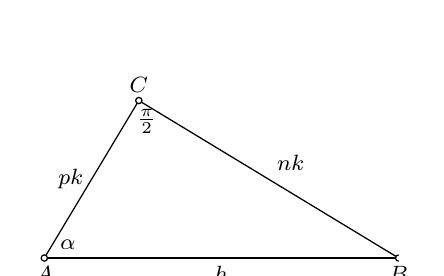
\begin{tikzpicture}
                            % \clip (0,0) rectangle (14.000000,10.000000);
                            {\footnotesize
                            
                            % Marking point C by circle
                            \draw [line width=0.016cm] (2.700000,3.500000) circle (0.040000);%
                            \draw (2.700000,3.500000) node [anchor=south] { $C$ };%
                            
                            % Marking point A by circle
                            \draw [line width=0.016cm] (1.500000,1.500000) circle (0.040000);%
                            \draw (1.500000,1.500000) node [anchor=north] { $A$ };%
                            
                            % Marking point B by circle
                            \draw [line width=0.016cm] (6.000000,1.540000) arc (90:269:0.040000 and 0.040000) -- (6.000000,1.460000);%
                            \draw (6.000000,1.500000) node [anchor=north] { $B$ };%
                            
                            % Drawing segment A C
                            \draw [line width=0.016cm] (1.520580,1.534300) -- (2.679420,3.465700);%
                            
                            % Drawing segment A B
                            \draw [line width=0.016cm] (1.540000,1.500000) -- (5.960000,1.500000);%
                            
                            % Drawing segment B C
                            \draw [line width=0.016cm] (5.965792,1.520732) -- (2.734208,3.479268);%
                            
                            % Marking point \alpha
                            \draw (1.800000,1.500000) node [anchor=south] { $\alpha$ };%
                            
                            % Marking point \frac{\pi}{2}
                            \draw (2.800000,3.500000) node [anchor=north] { $\frac{\pi}{2}$ };%
                            
                            % Marking point h
                            \draw (3.750000,1.500000) node [anchor=north] { $h$ };%
                            
                            % Marking point pk
                            \draw (2.100000,2.500000) node [anchor=east] { $pk$ };%
                            
                            % Marking point nk
                            \draw (4.350000,2.500000) node [anchor=south west] { $nk$ };%
                            }
                            \end{tikzpicture}
                        \end{figure}
                        ~\\
                        ~\\
                        \textbf{Kotangens} kota $\alpha$ je količnik med kotu $\alpha$ priležno kateto in nasprotno kateto: $$\cot\alpha = \frac{\textrm{priležna kateta}}{\textrm{nasprotna kateta}}.$$
            \end{columns}

        \end{frame}


        \begin{frame}
            \frametitle{Kotne funkcije komplementarnih kotov}

            \begin{alertblock}{}
                Sinus kota je enak kosinusu komplementarnega kota in obratno.
                $$ \sin\left({\frac{\pi}{2}-\varphi}\right) = \cos\varphi $$
                $$ \cos\left({\frac{\pi}{2}-\varphi}\right) = \sin\varphi $$
            \end{alertblock}

            \begin{alertblock}{}
                Tangens kota je enak kotangensu komplementarnega kota in obratno.
                $$ \tan\left({\frac{\pi}{2}-\varphi}\right) = \cot\varphi $$
                $$ \cot\left({\frac{\pi}{2}-\varphi}\right) = \tan\varphi $$
            \end{alertblock}
        \end{frame}
        

        \begin{frame}
            \frametitle{Kotne funkcije v enotskem krogu}

            \begin{columns}
                \column{0.43\textwidth}
                    \begin{alertblock}{}
                        \textbf{Enotska krožnica} je krožnica s polmerom ene enote in s središčem v koordinatnem izhodišču.
                    \end{alertblock}

                    \begin{alertblock}{}
                        Kot $\varphi$ z vrhom v koordinatnem izhodišču:
                        \begin{itemize}
                            \item prvi (fiksni) krak kota leži na pozitivnem delu abscisne osi;
                            \item drugi (premični) krak določa velikost kota in leži v enem izmed štirih kvadrantov.
                        \end{itemize}
                    \end{alertblock}

                \column{0.55\textwidth}
                    \begin{figure}
                        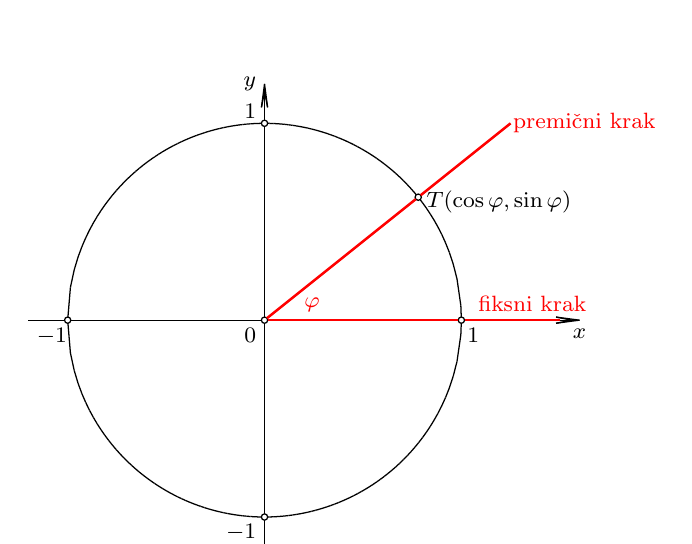
\begin{tikzpicture}
                            % \clip (0,0) rectangle (14.000000,10.000000);
                            {\footnotesize
                            
                            % Drawing 2D Cartesian system
                            \draw [line width=0.016cm] (3.000000,3.000000) circle (0.040000);%
                            \draw (3.000000,3.000000) node [anchor=north east] { $0$ };%
                            \draw [line width=0.016cm] (5.500000,3.000000) circle (0.040000);%
                            \draw (5.650000,3.000000) node [anchor=north] { $1$ };%
                            \draw [line width=0.016cm] (0.500000,3.000000) circle (0.040000);%
                            \draw (0.300000,3.000000) node [anchor=north] { $-1$ };%
                            \draw [line width=0.016cm] (3.000000,5.500000) circle (0.040000);%
                            \draw (3.000000,5.650000) node [anchor=east] { $1$ };%
                            \draw [line width=0.016cm] (3.000000,0.500000) circle (0.040000);%
                            \draw (3.000000,0.300000) node [anchor=east] { $-1$ };%
                            \draw (7.000000,3.000000) node [anchor=north] { $x$ };%
                            \draw (3.000000,6.000000) node [anchor=east] { $y$ };%
                            \draw [line width=0.016cm] (0.000000,3.000000) -- (0.460000,3.000000);%
                            \draw [line width=0.016cm] (0.540000,3.000000) -- (2.960000,3.000000);%
                            \draw [line width=0.016cm] (3.040000,3.000000) -- (5.460000,3.000000);%
                            \draw [line width=0.016cm] (5.540000,3.000000) -- (7.000000,3.000000);%
                            \draw [line width=0.016cm] (6.702567,3.039158) -- (7.000000,3.000000);%
                            \draw [line width=0.016cm] (6.702567,3.039158) -- (6.900000,3.000000);%
                            \draw [line width=0.016cm] (6.702567,2.960842) -- (7.000000,3.000000);%
                            \draw [line width=0.016cm] (6.702567,2.960842) -- (6.900000,3.000000);%
                            \draw [line width=0.016cm] (3.000000,0.000000) -- (3.000000,0.460000);%
                            \draw [line width=0.016cm] (3.000000,0.540000) -- (3.000000,2.960000);%
                            \draw [line width=0.016cm] (3.000000,3.040000) -- (3.000000,5.460000);%
                            \draw [line width=0.016cm] (3.000000,5.540000) -- (3.000000,6.000000);%
                            \draw [line width=0.016cm] (2.960842,5.702567) -- (3.000000,6.000000);%
                            \draw [line width=0.016cm] (2.960842,5.702567) -- (3.000000,5.900000);%
                            \draw [line width=0.016cm] (3.039158,5.702567) -- (3.000000,6.000000);%
                            \draw [line width=0.016cm] (3.039158,5.702567) -- (3.000000,5.900000);%
                            
                            % Drawing 2D ang conic k
                            \draw [line width=0.016cm] (0.503333,3.039861) -- (0.517361,3.207609);%
                            \draw [line width=0.016cm] (0.517361,3.207609) -- (0.534722,3.415217);%
                            \draw [line width=0.016cm] (0.503333,2.960139) -- (0.517361,2.792391);%
                            \draw [line width=0.016cm] (0.517361,2.792391) -- (0.534722,2.584783);%
                            \draw [line width=0.016cm] (0.534722,3.415217) -- (0.583333,3.640095);%
                            \draw [line width=0.016cm] (0.534722,2.584783) -- (0.583333,2.359905);%
                            \draw [line width=0.016cm] (0.583333,3.640095) -- (0.631944,3.801444);%
                            \draw [line width=0.016cm] (0.583333,2.359905) -- (0.631944,2.198556);%
                            \draw [line width=0.016cm] (0.631944,3.801444) -- (0.680556,3.932833);%
                            \draw [line width=0.016cm] (0.631944,2.198556) -- (0.680556,2.067167);%
                            \draw [line width=0.016cm] (0.680556,3.932833) -- (0.729167,4.045618);%
                            \draw [line width=0.016cm] (0.680556,2.067167) -- (0.729167,1.954382);%
                            \draw [line width=0.016cm] (0.729167,4.045618) -- (0.777778,4.145307);%
                            \draw [line width=0.016cm] (0.729167,1.954382) -- (0.777778,1.854693);%
                            \draw [line width=0.016cm] (0.777778,4.145307) -- (0.826389,4.235077);%
                            \draw [line width=0.016cm] (0.777778,1.854693) -- (0.826389,1.764923);%
                            \draw [line width=0.016cm] (0.826389,4.235077) -- (0.875000,4.316957);%
                            \draw [line width=0.016cm] (0.826389,1.764923) -- (0.875000,1.683043);%
                            \draw [line width=0.016cm] (0.875000,4.316957) -- (0.923611,4.392339);%
                            \draw [line width=0.016cm] (0.875000,1.683043) -- (0.923611,1.607661);%
                            \draw [line width=0.016cm] (0.923611,4.392339) -- (0.972222,4.462230);%
                            \draw [line width=0.016cm] (0.923611,1.607661) -- (0.972222,1.537770);%
                            \draw [line width=0.016cm] (0.972222,4.462230) -- (1.020833,4.527383);%
                            \draw [line width=0.016cm] (0.972222,1.537770) -- (1.020833,1.472617);%
                            \draw [line width=0.016cm] (1.020833,4.527383) -- (1.069444,4.588381);%
                            \draw [line width=0.016cm] (1.020833,1.472617) -- (1.069444,1.411619);%
                            \draw [line width=0.016cm] (1.069444,4.588381) -- (1.118056,4.645687);%
                            \draw [line width=0.016cm] (1.069444,1.411619) -- (1.118056,1.354313);%
                            \draw [line width=0.016cm] (1.118056,4.645687) -- (1.166667,4.699673);%
                            \draw [line width=0.016cm] (1.118056,1.354313) -- (1.166667,1.300327);%
                            \draw [line width=0.016cm] (1.166667,4.699673) -- (1.215278,4.750647);%
                            \draw [line width=0.016cm] (1.166667,1.300327) -- (1.215278,1.249353);%
                            \draw [line width=0.016cm] (1.215278,4.750647) -- (1.263889,4.798866);%
                            \draw [line width=0.016cm] (1.215278,1.249353) -- (1.263889,1.201134);%
                            \draw [line width=0.016cm] (1.263889,4.798866) -- (1.312500,4.844544);%
                            \draw [line width=0.016cm] (1.263889,1.201134) -- (1.312500,1.155456);%
                            \draw [line width=0.016cm] (1.312500,4.844544) -- (1.361111,4.887867);%
                            \draw [line width=0.016cm] (1.312500,1.155456) -- (1.361111,1.112133);%
                            \draw [line width=0.016cm] (1.361111,4.887867) -- (1.409722,4.928994);%
                            \draw [line width=0.016cm] (1.361111,1.112133) -- (1.409722,1.071006);%
                            \draw [line width=0.016cm] (1.409722,4.928994) -- (1.458333,4.968061);%
                            \draw [line width=0.016cm] (1.409722,1.071006) -- (1.458333,1.031939);%
                            \draw [line width=0.016cm] (1.458333,4.968061) -- (1.506944,5.005190);%
                            \draw [line width=0.016cm] (1.458333,1.031939) -- (1.506944,0.994810);%
                            \draw [line width=0.016cm] (1.506944,5.005190) -- (1.555556,5.040485);%
                            \draw [line width=0.016cm] (1.506944,0.994810) -- (1.555556,0.959515);%
                            \draw [line width=0.016cm] (1.555556,5.040485) -- (1.604167,5.074042);%
                            \draw [line width=0.016cm] (1.555556,0.959515) -- (1.604167,0.925958);%
                            \draw [line width=0.016cm] (1.604167,5.074042) -- (1.652778,5.105942);%
                            \draw [line width=0.016cm] (1.604167,0.925958) -- (1.652778,0.894058);%
                            \draw [line width=0.016cm] (1.652778,5.105942) -- (1.701389,5.136261);%
                            \draw [line width=0.016cm] (1.652778,0.894058) -- (1.701389,0.863739);%
                            \draw [line width=0.016cm] (1.701389,5.136261) -- (1.750000,5.165064);%
                            \draw [line width=0.016cm] (1.701389,0.863739) -- (1.750000,0.834936);%
                            \draw [line width=0.016cm] (1.750000,5.165064) -- (1.798611,5.192411);%
                            \draw [line width=0.016cm] (1.750000,0.834936) -- (1.798611,0.807589);%
                            \draw [line width=0.016cm] (1.798611,5.192411) -- (1.847222,5.218356);%
                            \draw [line width=0.016cm] (1.798611,0.807589) -- (1.847222,0.781644);%
                            \draw [line width=0.016cm] (1.847222,5.218356) -- (1.895833,5.242948);%
                            \draw [line width=0.016cm] (1.847222,0.781644) -- (1.895833,0.757052);%
                            \draw [line width=0.016cm] (1.895833,5.242948) -- (1.944444,5.266231);%
                            \draw [line width=0.016cm] (1.895833,0.757052) -- (1.944444,0.733769);%
                            \draw [line width=0.016cm] (1.944444,5.266231) -- (1.993056,5.288244);%
                            \draw [line width=0.016cm] (1.944444,0.733769) -- (1.993056,0.711756);%
                            \draw [line width=0.016cm] (1.993056,5.288244) -- (2.041667,5.309025);%
                            \draw [line width=0.016cm] (1.993056,0.711756) -- (2.041667,0.690975);%
                            \draw [line width=0.016cm] (2.041667,5.309025) -- (2.090278,5.328606);%
                            \draw [line width=0.016cm] (2.041667,0.690975) -- (2.090278,0.671394);%
                            \draw [line width=0.016cm] (2.090278,5.328606) -- (2.138889,5.347017);%
                            \draw [line width=0.016cm] (2.090278,0.671394) -- (2.138889,0.652983);%
                            \draw [line width=0.016cm] (2.138889,5.347017) -- (2.187500,5.364285);%
                            \draw [line width=0.016cm] (2.138889,0.652983) -- (2.187500,0.635715);%
                            \draw [line width=0.016cm] (2.187500,5.364285) -- (2.236111,5.380436);%
                            \draw [line width=0.016cm] (2.187500,0.635715) -- (2.236111,0.619564);%
                            \draw [line width=0.016cm] (2.236111,5.380436) -- (2.284722,5.395491);%
                            \draw [line width=0.016cm] (2.236111,0.619564) -- (2.284722,0.604509);%
                            \draw [line width=0.016cm] (2.284722,5.395491) -- (2.333333,5.409472);%
                            \draw [line width=0.016cm] (2.284722,0.604509) -- (2.333333,0.590528);%
                            \draw [line width=0.016cm] (2.333333,5.409472) -- (2.381944,5.422397);%
                            \draw [line width=0.016cm] (2.333333,0.590528) -- (2.381944,0.577603);%
                            \draw [line width=0.016cm] (2.381944,5.422397) -- (2.430556,5.434283);%
                            \draw [line width=0.016cm] (2.381944,0.577603) -- (2.430556,0.565717);%
                            \draw [line width=0.016cm] (2.430556,5.434283) -- (2.479167,5.445145);%
                            \draw [line width=0.016cm] (2.430556,0.565717) -- (2.479167,0.554855);%
                            \draw [line width=0.016cm] (2.479167,5.445145) -- (2.527778,5.454996);%
                            \draw [line width=0.016cm] (2.479167,0.554855) -- (2.527778,0.545004);%
                            \draw [line width=0.016cm] (2.527778,5.454996) -- (2.576389,5.463849);%
                            \draw [line width=0.016cm] (2.527778,0.545004) -- (2.576389,0.536151);%
                            \draw [line width=0.016cm] (2.576389,5.463849) -- (2.625000,5.471715);%
                            \draw [line width=0.016cm] (2.576389,0.536151) -- (2.625000,0.528285);%
                            \draw [line width=0.016cm] (2.625000,5.471715) -- (2.673611,5.478602);%
                            \draw [line width=0.016cm] (2.625000,0.528285) -- (2.673611,0.521398);%
                            \draw [line width=0.016cm] (2.673611,5.478602) -- (2.722222,5.484520);%
                            \draw [line width=0.016cm] (2.673611,0.521398) -- (2.722222,0.515480);%
                            \draw [line width=0.016cm] (2.722222,5.484520) -- (2.770833,5.489474);%
                            \draw [line width=0.016cm] (2.722222,0.515480) -- (2.770833,0.510526);%
                            \draw [line width=0.016cm] (2.770833,5.489474) -- (2.819444,5.493471);%
                            \draw [line width=0.016cm] (2.770833,0.510526) -- (2.819444,0.506529);%
                            \draw [line width=0.016cm] (2.819444,5.493471) -- (2.868056,5.496516);%
                            \draw [line width=0.016cm] (2.819444,0.506529) -- (2.868056,0.503484);%
                            \draw [line width=0.016cm] (2.868056,5.496516) -- (2.916667,5.498611);%
                            \draw [line width=0.016cm] (2.868056,0.503484) -- (2.916667,0.501389);%
                            \draw [line width=0.016cm] (2.916667,5.498611) -- (2.960002,5.499634);%
                            \draw [line width=0.016cm] (2.916667,0.501389) -- (2.960002,0.500366);%
                            \draw [line width=0.016cm] (3.039998,5.499562) -- (3.062500,5.499219);%
                            \draw [line width=0.016cm] (3.039998,0.500438) -- (3.062500,0.500781);%
                            \draw [line width=0.016cm] (3.062500,5.499219) -- (3.111111,5.497530);%
                            \draw [line width=0.016cm] (3.062500,0.500781) -- (3.111111,0.502470);%
                            \draw [line width=0.016cm] (3.111111,5.497530) -- (3.159722,5.494893);%
                            \draw [line width=0.016cm] (3.111111,0.502470) -- (3.159722,0.505107);%
                            \draw [line width=0.016cm] (3.159722,5.494893) -- (3.208333,5.491304);%
                            \draw [line width=0.016cm] (3.159722,0.505107) -- (3.208333,0.508696);%
                            \draw [line width=0.016cm] (3.208333,5.491304) -- (3.256944,5.486761);%
                            \draw [line width=0.016cm] (3.208333,0.508696) -- (3.256944,0.513239);%
                            \draw [line width=0.016cm] (3.256944,5.486761) -- (3.305556,5.481257);%
                            \draw [line width=0.016cm] (3.256944,0.513239) -- (3.305556,0.518743);%
                            \draw [line width=0.016cm] (3.305556,5.481257) -- (3.354167,5.474786);%
                            \draw [line width=0.016cm] (3.305556,0.518743) -- (3.354167,0.525214);%
                            \draw [line width=0.016cm] (3.354167,5.474786) -- (3.402778,5.467341);%
                            \draw [line width=0.016cm] (3.354167,0.525214) -- (3.402778,0.532659);%
                            \draw [line width=0.016cm] (3.402778,5.467341) -- (3.451389,5.458912);%
                            \draw [line width=0.016cm] (3.402778,0.532659) -- (3.451389,0.541088);%
                            \draw [line width=0.016cm] (3.451389,5.458912) -- (3.500000,5.449490);%
                            \draw [line width=0.016cm] (3.451389,0.541088) -- (3.500000,0.550510);%
                            \draw [line width=0.016cm] (3.500000,5.449490) -- (3.548611,5.439062);%
                            \draw [line width=0.016cm] (3.500000,0.550510) -- (3.548611,0.560938);%
                            \draw [line width=0.016cm] (3.548611,5.439062) -- (3.597222,5.427617);%
                            \draw [line width=0.016cm] (3.548611,0.560938) -- (3.597222,0.572383);%
                            \draw [line width=0.016cm] (3.597222,5.427617) -- (3.645833,5.415140);%
                            \draw [line width=0.016cm] (3.597222,0.572383) -- (3.645833,0.584860);%
                            \draw [line width=0.016cm] (3.645833,5.415140) -- (3.694444,5.401613);%
                            \draw [line width=0.016cm] (3.645833,0.584860) -- (3.694444,0.598387);%
                            \draw [line width=0.016cm] (3.694444,5.401613) -- (3.743056,5.387021);%
                            \draw [line width=0.016cm] (3.694444,0.598387) -- (3.743056,0.612979);%
                            \draw [line width=0.016cm] (3.743056,5.387021) -- (3.791667,5.371342);%
                            \draw [line width=0.016cm] (3.743056,0.612979) -- (3.791667,0.628658);%
                            \draw [line width=0.016cm] (3.791667,5.371342) -- (3.840278,5.354556);%
                            \draw [line width=0.016cm] (3.791667,0.628658) -- (3.840278,0.645444);%
                            \draw [line width=0.016cm] (3.840278,5.354556) -- (3.888889,5.336638);%
                            \draw [line width=0.016cm] (3.840278,0.645444) -- (3.888889,0.663362);%
                            \draw [line width=0.016cm] (3.888889,5.336638) -- (3.937500,5.317562);%
                            \draw [line width=0.016cm] (3.888889,0.663362) -- (3.937500,0.682438);%
                            \draw [line width=0.016cm] (3.937500,5.317562) -- (3.986111,5.297299);%
                            \draw [line width=0.016cm] (3.937500,0.682438) -- (3.986111,0.702701);%
                            \draw [line width=0.016cm] (3.986111,5.297299) -- (4.034722,5.275819);%
                            \draw [line width=0.016cm] (3.986111,0.702701) -- (4.034722,0.724181);%
                            \draw [line width=0.016cm] (4.034722,5.275819) -- (4.083333,5.253084);%
                            \draw [line width=0.016cm] (4.034722,0.724181) -- (4.083333,0.746916);%
                            \draw [line width=0.016cm] (4.083333,5.253084) -- (4.131944,5.229058);%
                            \draw [line width=0.016cm] (4.083333,0.746916) -- (4.131944,0.770942);%
                            \draw [line width=0.016cm] (4.131944,5.229058) -- (4.180556,5.203699);%
                            \draw [line width=0.016cm] (4.131944,0.770942) -- (4.180556,0.796301);%
                            \draw [line width=0.016cm] (4.180556,5.203699) -- (4.229167,5.176959);%
                            \draw [line width=0.016cm] (4.180556,0.796301) -- (4.229167,0.823041);%
                            \draw [line width=0.016cm] (4.229167,5.176959) -- (4.277778,5.148787);%
                            \draw [line width=0.016cm] (4.229167,0.823041) -- (4.277778,0.851213);%
                            \draw [line width=0.016cm] (4.277778,5.148787) -- (4.326389,5.119125);%
                            \draw [line width=0.016cm] (4.277778,0.851213) -- (4.326389,0.880875);%
                            \draw [line width=0.016cm] (4.326389,5.119125) -- (4.375000,5.087912);%
                            \draw [line width=0.016cm] (4.326389,0.880875) -- (4.375000,0.912088);%
                            \draw [line width=0.016cm] (4.375000,5.087912) -- (4.423611,5.055075);%
                            \draw [line width=0.016cm] (4.375000,0.912088) -- (4.423611,0.944925);%
                            \draw [line width=0.016cm] (4.423611,5.055075) -- (4.472222,5.020535);%
                            \draw [line width=0.016cm] (4.423611,0.944925) -- (4.472222,0.979465);%
                            \draw [line width=0.016cm] (4.472222,5.020535) -- (4.520833,4.984204);%
                            \draw [line width=0.016cm] (4.472222,0.979465) -- (4.520833,1.015796);%
                            \draw [line width=0.016cm] (4.520833,4.984204) -- (4.569444,4.945982);%
                            \draw [line width=0.016cm] (4.520833,1.015796) -- (4.569444,1.054018);%
                            \draw [line width=0.016cm] (4.569444,4.945982) -- (4.618056,4.905753);%
                            \draw [line width=0.016cm] (4.569444,1.054018) -- (4.618056,1.094247);%
                            \draw [line width=0.016cm] (4.618056,4.905753) -- (4.666667,4.863390);%
                            \draw [line width=0.016cm] (4.618056,1.094247) -- (4.666667,1.136610);%
                            \draw [line width=0.016cm] (4.666667,4.863390) -- (4.715278,4.818742);%
                            \draw [line width=0.016cm] (4.666667,1.136610) -- (4.715278,1.181258);%
                            \draw [line width=0.016cm] (4.715278,4.818742) -- (4.763889,4.771637);%
                            \draw [line width=0.016cm] (4.715278,1.181258) -- (4.763889,1.228363);%
                            \draw [line width=0.016cm] (4.763889,4.771637) -- (4.812500,4.721872);%
                            \draw [line width=0.016cm] (4.763889,1.228363) -- (4.812500,1.278128);%
                            \draw [line width=0.016cm] (4.812500,4.721872) -- (4.861111,4.669211);%
                            \draw [line width=0.016cm] (4.812500,1.278128) -- (4.861111,1.330789);%
                            \draw [line width=0.016cm] (4.861111,4.669211) -- (4.909722,4.613369);%
                            \draw [line width=0.016cm] (4.861111,1.330789) -- (4.909722,1.386631);%
                            \draw [line width=0.016cm] (4.909722,4.613369) -- (4.926728,4.592602);%
                            \draw [line width=0.016cm] (4.909722,1.386631) -- (4.958333,1.445995);%
                            \draw [line width=0.016cm] (4.976673,4.530120) -- (5.006944,4.490696);%
                            \draw [line width=0.016cm] (4.958333,1.445995) -- (5.006944,1.509304);%
                            \draw [line width=0.016cm] (5.006944,4.490696) -- (5.055556,4.422916);%
                            \draw [line width=0.016cm] (5.006944,1.509304) -- (5.055556,1.577084);%
                            \draw [line width=0.016cm] (5.055556,4.422916) -- (5.104167,4.349994);%
                            \draw [line width=0.016cm] (5.055556,1.577084) -- (5.104167,1.650006);%
                            \draw [line width=0.016cm] (5.104167,4.349994) -- (5.152778,4.271042);%
                            \draw [line width=0.016cm] (5.104167,1.650006) -- (5.152778,1.728958);%
                            \draw [line width=0.016cm] (5.152778,4.271042) -- (5.201389,4.184857);%
                            \draw [line width=0.016cm] (5.152778,1.728958) -- (5.201389,1.815143);%
                            \draw [line width=0.016cm] (5.201389,4.184857) -- (5.250000,4.089725);%
                            \draw [line width=0.016cm] (5.201389,1.815143) -- (5.250000,1.910275);%
                            \draw [line width=0.016cm] (5.250000,4.089725) -- (5.298611,3.983050);%
                            \draw [line width=0.016cm] (5.250000,1.910275) -- (5.298611,2.016950);%
                            \draw [line width=0.016cm] (5.298611,3.983050) -- (5.347222,3.860551);%
                            \draw [line width=0.016cm] (5.298611,2.016950) -- (5.347222,2.139449);%
                            \draw [line width=0.016cm] (5.347222,3.860551) -- (5.395833,3.714131);%
                            \draw [line width=0.016cm] (5.347222,2.139449) -- (5.395833,2.285869);%
                            \draw [line width=0.016cm] (5.395833,3.714131) -- (5.444444,3.524110);%
                            \draw [line width=0.016cm] (5.395833,2.285869) -- (5.444444,2.475890);%
                            \draw [line width=0.016cm] (5.444444,3.524110) -- (5.493056,3.186210);%
                            \draw [line width=0.016cm] (5.444444,2.475890) -- (5.493056,2.813790);%
                            \draw [line width=0.016cm] (5.498509,3.039972) -- (5.496528,3.093105);%
                            \draw [line width=0.016cm] (5.496528,3.093105) -- (5.493056,3.186210);%
                            \draw [line width=0.016cm] (5.498509,2.960028) -- (5.496528,2.906895);%
                            \draw [line width=0.016cm] (5.496528,2.906895) -- (5.493056,2.813790);%
                            
                            % Marking point T(\cos\varphi,\sin\varphi) by circle
                            \draw [line width=0.016cm] (4.952172,4.561738) circle (0.040000);%
                            \draw (4.952172,4.500000) node [anchor=west] { $T(\cos\varphi,\sin\varphi)$ };%
                            
                            % Changing color 255 0 0
                            \definecolor{r255g0b0}{rgb}{1.000000,0.000000,0.000000}%
                            \color{r255g0b0}% 
                            
                            % Marking point \textrm{fiksni~krak}
                            \draw (6.400000,3.000000) node [anchor=south] { $\textrm{fiksni~krak}$ };%
                            
                            % Marking point \textrm{premični~krak}
                            \draw (6.050000,5.500000) node [anchor=west] { $\textrm{premični~krak}$ };%

                            % Drawing segment S L
                            \draw [line width=0.032cm] (3.040000,3.000000) -- (5.460000,3.000000);%
                            \draw [line width=0.032cm] (5.540000,3.000000) -- (6.750000,3.000000);%

                            % Drawing segment S X
                            \draw [line width=0.032cm] (3.031235,3.024988) -- (4.920937,4.536750);%
                            \draw [line width=0.032cm] (4.983407,4.586725) -- (6.125000,5.500000);%

                            % Marking point \varphi
                            \draw (3.400000,3.000000) node [anchor=south west] { $\varphi$ };%
                            \color{black}
                            }
                        \end{tikzpicture}
                    \end{figure}
            \end{columns}
            ~\\
            ~\\




        \end{frame}

        \begin{frame}

            \begin{columns}
                \column{0.43\textwidth}
                    \begin{alertblock}{}
                        \textbf{Sinus} kota $\varphi$ je enak oridnati presečišča premičnega kraka z enotsko krožnico.
                    \end{alertblock}

                    \begin{alertblock}{}
                        \textbf{Kosinus} kota $\varphi$ je enak abscisi presečišča premičnega kraka z enotsko krožnico.
                    \end{alertblock}

                    \begin{alertblock}{}
                        \textbf{Tangens} kota $\varphi$ je enak ordinati presečišča premičnega kraka z navpično tangento enotskega kroga v točki $(1,0)$.
                    \end{alertblock}

                    \begin{alertblock}{}
                        \textbf{Kotangens} kota $\varphi$ je enak abscisi presečišča premičnega kraka z vodoravno tangento enotskega korga v točko $(0,1)$.
                    \end{alertblock}

                \column{0.55\textwidth}
                    \begin{figure}
                        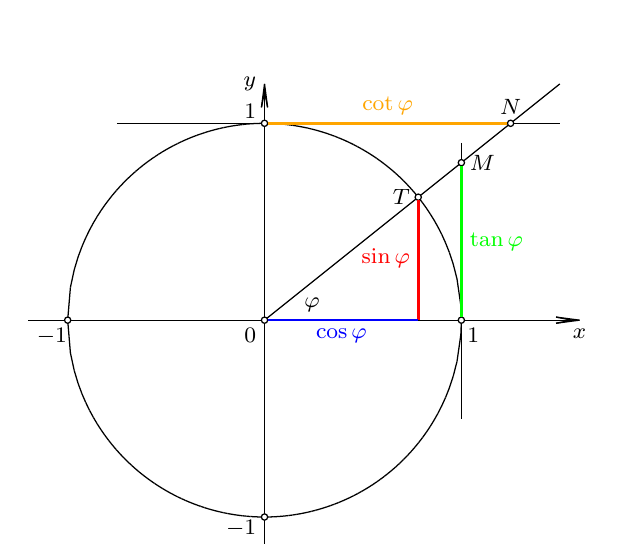
\begin{tikzpicture}
                            % \clip (0,0) rectangle (14.000000,10.000000);
                            {\footnotesize
                            
                            % Drawing 2D Cartesian system
                            \draw [line width=0.016cm] (3.000000,3.000000) circle (0.040000);%
                            \draw (3.000000,3.000000) node [anchor=north east] { $0$ };%
                            \draw [line width=0.016cm] (5.500000,3.000000) circle (0.040000);%
                            \draw (5.650000,3.000000) node [anchor=north] { $1$ };%
                            \draw [line width=0.016cm] (0.500000,3.000000) circle (0.040000);%
                            \draw (0.300000,3.000000) node [anchor=north] { $-1$ };%
                            \draw [line width=0.016cm] (3.000000,5.500000) circle (0.040000);%
                            \draw (3.000000,5.650000) node [anchor=east] { $1$ };%
                            \draw [line width=0.016cm] (3.000000,0.500000) circle (0.040000);%
                            \draw (3.000000,0.350000) node [anchor=east] { $-1$ };%
                            \draw (7.000000,3.000000) node [anchor=north] { $x$ };%
                            \draw (3.000000,6.000000) node [anchor=east] { $y$ };%
                            \draw [line width=0.016cm] (0.000000,3.000000) -- (0.460000,3.000000);%
                            \draw [line width=0.016cm] (0.540000,3.000000) -- (2.960000,3.000000);%
                            \draw [line width=0.016cm] (3.040000,3.000000) -- (5.460000,3.000000);%
                            \draw [line width=0.016cm] (5.540000,3.000000) -- (7.000000,3.000000);%
                            \draw [line width=0.016cm] (6.702567,3.039158) -- (7.000000,3.000000);%
                            \draw [line width=0.016cm] (6.702567,3.039158) -- (6.900000,3.000000);%
                            \draw [line width=0.016cm] (6.702567,2.960842) -- (7.000000,3.000000);%
                            \draw [line width=0.016cm] (6.702567,2.960842) -- (6.900000,3.000000);%
                            \draw [line width=0.016cm] (3.000000,0.000000) -- (3.000000,0.460000);%
                            \draw [line width=0.016cm] (3.000000,0.540000) -- (3.000000,2.960000);%
                            \draw [line width=0.016cm] (3.000000,3.040000) -- (3.000000,5.460000);%
                            \draw [line width=0.016cm] (3.000000,5.540000) -- (3.000000,6.000000);%
                            \draw [line width=0.016cm] (2.960842,5.702567) -- (3.000000,6.000000);%
                            \draw [line width=0.016cm] (2.960842,5.702567) -- (3.000000,5.900000);%
                            \draw [line width=0.016cm] (3.039158,5.702567) -- (3.000000,6.000000);%
                            \draw [line width=0.016cm] (3.039158,5.702567) -- (3.000000,5.900000);%
                            
                            % Drawing 2D ang conic k
                            \draw [line width=0.016cm] (0.503333,3.039861) -- (0.517361,3.207609);%
                            \draw [line width=0.016cm] (0.517361,3.207609) -- (0.534722,3.415217);%
                            \draw [line width=0.016cm] (0.503333,2.960139) -- (0.517361,2.792391);%
                            \draw [line width=0.016cm] (0.517361,2.792391) -- (0.534722,2.584783);%
                            \draw [line width=0.016cm] (0.534722,3.415217) -- (0.583333,3.640095);%
                            \draw [line width=0.016cm] (0.534722,2.584783) -- (0.583333,2.359905);%
                            \draw [line width=0.016cm] (0.583333,3.640095) -- (0.631944,3.801444);%
                            \draw [line width=0.016cm] (0.583333,2.359905) -- (0.631944,2.198556);%
                            \draw [line width=0.016cm] (0.631944,3.801444) -- (0.680556,3.932833);%
                            \draw [line width=0.016cm] (0.631944,2.198556) -- (0.680556,2.067167);%
                            \draw [line width=0.016cm] (0.680556,3.932833) -- (0.729167,4.045618);%
                            \draw [line width=0.016cm] (0.680556,2.067167) -- (0.729167,1.954382);%
                            \draw [line width=0.016cm] (0.729167,4.045618) -- (0.777778,4.145307);%
                            \draw [line width=0.016cm] (0.729167,1.954382) -- (0.777778,1.854693);%
                            \draw [line width=0.016cm] (0.777778,4.145307) -- (0.826389,4.235077);%
                            \draw [line width=0.016cm] (0.777778,1.854693) -- (0.826389,1.764923);%
                            \draw [line width=0.016cm] (0.826389,4.235077) -- (0.875000,4.316957);%
                            \draw [line width=0.016cm] (0.826389,1.764923) -- (0.875000,1.683043);%
                            \draw [line width=0.016cm] (0.875000,4.316957) -- (0.923611,4.392339);%
                            \draw [line width=0.016cm] (0.875000,1.683043) -- (0.923611,1.607661);%
                            \draw [line width=0.016cm] (0.923611,4.392339) -- (0.972222,4.462230);%
                            \draw [line width=0.016cm] (0.923611,1.607661) -- (0.972222,1.537770);%
                            \draw [line width=0.016cm] (0.972222,4.462230) -- (1.020833,4.527383);%
                            \draw [line width=0.016cm] (0.972222,1.537770) -- (1.020833,1.472617);%
                            \draw [line width=0.016cm] (1.020833,4.527383) -- (1.069444,4.588381);%
                            \draw [line width=0.016cm] (1.020833,1.472617) -- (1.069444,1.411619);%
                            \draw [line width=0.016cm] (1.069444,4.588381) -- (1.118056,4.645687);%
                            \draw [line width=0.016cm] (1.069444,1.411619) -- (1.118056,1.354313);%
                            \draw [line width=0.016cm] (1.118056,4.645687) -- (1.166667,4.699673);%
                            \draw [line width=0.016cm] (1.118056,1.354313) -- (1.166667,1.300327);%
                            \draw [line width=0.016cm] (1.166667,4.699673) -- (1.215278,4.750647);%
                            \draw [line width=0.016cm] (1.166667,1.300327) -- (1.215278,1.249353);%
                            \draw [line width=0.016cm] (1.215278,4.750647) -- (1.263889,4.798866);%
                            \draw [line width=0.016cm] (1.215278,1.249353) -- (1.263889,1.201134);%
                            \draw [line width=0.016cm] (1.263889,4.798866) -- (1.312500,4.844544);%
                            \draw [line width=0.016cm] (1.263889,1.201134) -- (1.312500,1.155456);%
                            \draw [line width=0.016cm] (1.312500,4.844544) -- (1.361111,4.887867);%
                            \draw [line width=0.016cm] (1.312500,1.155456) -- (1.361111,1.112133);%
                            \draw [line width=0.016cm] (1.361111,4.887867) -- (1.409722,4.928994);%
                            \draw [line width=0.016cm] (1.361111,1.112133) -- (1.409722,1.071006);%
                            \draw [line width=0.016cm] (1.409722,4.928994) -- (1.458333,4.968061);%
                            \draw [line width=0.016cm] (1.409722,1.071006) -- (1.458333,1.031939);%
                            \draw [line width=0.016cm] (1.458333,4.968061) -- (1.506944,5.005190);%
                            \draw [line width=0.016cm] (1.458333,1.031939) -- (1.506944,0.994810);%
                            \draw [line width=0.016cm] (1.506944,5.005190) -- (1.555556,5.040485);%
                            \draw [line width=0.016cm] (1.506944,0.994810) -- (1.555556,0.959515);%
                            \draw [line width=0.016cm] (1.555556,5.040485) -- (1.604167,5.074042);%
                            \draw [line width=0.016cm] (1.555556,0.959515) -- (1.604167,0.925958);%
                            \draw [line width=0.016cm] (1.604167,5.074042) -- (1.652778,5.105942);%
                            \draw [line width=0.016cm] (1.604167,0.925958) -- (1.652778,0.894058);%
                            \draw [line width=0.016cm] (1.652778,5.105942) -- (1.701389,5.136261);%
                            \draw [line width=0.016cm] (1.652778,0.894058) -- (1.701389,0.863739);%
                            \draw [line width=0.016cm] (1.701389,5.136261) -- (1.750000,5.165064);%
                            \draw [line width=0.016cm] (1.701389,0.863739) -- (1.750000,0.834936);%
                            \draw [line width=0.016cm] (1.750000,5.165064) -- (1.798611,5.192411);%
                            \draw [line width=0.016cm] (1.750000,0.834936) -- (1.798611,0.807589);%
                            \draw [line width=0.016cm] (1.798611,5.192411) -- (1.847222,5.218356);%
                            \draw [line width=0.016cm] (1.798611,0.807589) -- (1.847222,0.781644);%
                            \draw [line width=0.016cm] (1.847222,5.218356) -- (1.895833,5.242948);%
                            \draw [line width=0.016cm] (1.847222,0.781644) -- (1.895833,0.757052);%
                            \draw [line width=0.016cm] (1.895833,5.242948) -- (1.944444,5.266231);%
                            \draw [line width=0.016cm] (1.895833,0.757052) -- (1.944444,0.733769);%
                            \draw [line width=0.016cm] (1.944444,5.266231) -- (1.993056,5.288244);%
                            \draw [line width=0.016cm] (1.944444,0.733769) -- (1.993056,0.711756);%
                            \draw [line width=0.016cm] (1.993056,5.288244) -- (2.041667,5.309025);%
                            \draw [line width=0.016cm] (1.993056,0.711756) -- (2.041667,0.690975);%
                            \draw [line width=0.016cm] (2.041667,5.309025) -- (2.090278,5.328606);%
                            \draw [line width=0.016cm] (2.041667,0.690975) -- (2.090278,0.671394);%
                            \draw [line width=0.016cm] (2.090278,5.328606) -- (2.138889,5.347017);%
                            \draw [line width=0.016cm] (2.090278,0.671394) -- (2.138889,0.652983);%
                            \draw [line width=0.016cm] (2.138889,5.347017) -- (2.187500,5.364285);%
                            \draw [line width=0.016cm] (2.138889,0.652983) -- (2.187500,0.635715);%
                            \draw [line width=0.016cm] (2.187500,5.364285) -- (2.236111,5.380436);%
                            \draw [line width=0.016cm] (2.187500,0.635715) -- (2.236111,0.619564);%
                            \draw [line width=0.016cm] (2.236111,5.380436) -- (2.284722,5.395491);%
                            \draw [line width=0.016cm] (2.236111,0.619564) -- (2.284722,0.604509);%
                            \draw [line width=0.016cm] (2.284722,5.395491) -- (2.333333,5.409472);%
                            \draw [line width=0.016cm] (2.284722,0.604509) -- (2.333333,0.590528);%
                            \draw [line width=0.016cm] (2.333333,5.409472) -- (2.381944,5.422397);%
                            \draw [line width=0.016cm] (2.333333,0.590528) -- (2.381944,0.577603);%
                            \draw [line width=0.016cm] (2.381944,5.422397) -- (2.430556,5.434283);%
                            \draw [line width=0.016cm] (2.381944,0.577603) -- (2.430556,0.565717);%
                            \draw [line width=0.016cm] (2.430556,5.434283) -- (2.479167,5.445145);%
                            \draw [line width=0.016cm] (2.430556,0.565717) -- (2.479167,0.554855);%
                            \draw [line width=0.016cm] (2.479167,5.445145) -- (2.527778,5.454996);%
                            \draw [line width=0.016cm] (2.479167,0.554855) -- (2.527778,0.545004);%
                            \draw [line width=0.016cm] (2.527778,5.454996) -- (2.576389,5.463849);%
                            \draw [line width=0.016cm] (2.527778,0.545004) -- (2.576389,0.536151);%
                            \draw [line width=0.016cm] (2.576389,5.463849) -- (2.625000,5.471715);%
                            \draw [line width=0.016cm] (2.576389,0.536151) -- (2.625000,0.528285);%
                            \draw [line width=0.016cm] (2.625000,5.471715) -- (2.673611,5.478602);%
                            \draw [line width=0.016cm] (2.625000,0.528285) -- (2.673611,0.521398);%
                            \draw [line width=0.016cm] (2.673611,5.478602) -- (2.722222,5.484520);%
                            \draw [line width=0.016cm] (2.673611,0.521398) -- (2.722222,0.515480);%
                            \draw [line width=0.016cm] (2.722222,5.484520) -- (2.770833,5.489474);%
                            \draw [line width=0.016cm] (2.722222,0.515480) -- (2.770833,0.510526);%
                            \draw [line width=0.016cm] (2.770833,5.489474) -- (2.819444,5.493471);%
                            \draw [line width=0.016cm] (2.770833,0.510526) -- (2.819444,0.506529);%
                            \draw [line width=0.016cm] (2.819444,5.493471) -- (2.868056,5.496516);%
                            \draw [line width=0.016cm] (2.819444,0.506529) -- (2.868056,0.503484);%
                            \draw [line width=0.016cm] (2.868056,5.496516) -- (2.916667,5.498611);%
                            \draw [line width=0.016cm] (2.868056,0.503484) -- (2.916667,0.501389);%
                            \draw [line width=0.016cm] (2.916667,5.498611) -- (2.960002,5.499634);%
                            \draw [line width=0.016cm] (2.916667,0.501389) -- (2.960002,0.500366);%
                            \draw [line width=0.016cm] (3.039998,5.499562) -- (3.062500,5.499219);%
                            \draw [line width=0.016cm] (3.039998,0.500438) -- (3.062500,0.500781);%
                            \draw [line width=0.016cm] (3.062500,5.499219) -- (3.111111,5.497530);%
                            \draw [line width=0.016cm] (3.062500,0.500781) -- (3.111111,0.502470);%
                            \draw [line width=0.016cm] (3.111111,5.497530) -- (3.159722,5.494893);%
                            \draw [line width=0.016cm] (3.111111,0.502470) -- (3.159722,0.505107);%
                            \draw [line width=0.016cm] (3.159722,5.494893) -- (3.208333,5.491304);%
                            \draw [line width=0.016cm] (3.159722,0.505107) -- (3.208333,0.508696);%
                            \draw [line width=0.016cm] (3.208333,5.491304) -- (3.256944,5.486761);%
                            \draw [line width=0.016cm] (3.208333,0.508696) -- (3.256944,0.513239);%
                            \draw [line width=0.016cm] (3.256944,5.486761) -- (3.305556,5.481257);%
                            \draw [line width=0.016cm] (3.256944,0.513239) -- (3.305556,0.518743);%
                            \draw [line width=0.016cm] (3.305556,5.481257) -- (3.354167,5.474786);%
                            \draw [line width=0.016cm] (3.305556,0.518743) -- (3.354167,0.525214);%
                            \draw [line width=0.016cm] (3.354167,5.474786) -- (3.402778,5.467341);%
                            \draw [line width=0.016cm] (3.354167,0.525214) -- (3.402778,0.532659);%
                            \draw [line width=0.016cm] (3.402778,5.467341) -- (3.451389,5.458912);%
                            \draw [line width=0.016cm] (3.402778,0.532659) -- (3.451389,0.541088);%
                            \draw [line width=0.016cm] (3.451389,5.458912) -- (3.500000,5.449490);%
                            \draw [line width=0.016cm] (3.451389,0.541088) -- (3.500000,0.550510);%
                            \draw [line width=0.016cm] (3.500000,5.449490) -- (3.548611,5.439062);%
                            \draw [line width=0.016cm] (3.500000,0.550510) -- (3.548611,0.560938);%
                            \draw [line width=0.016cm] (3.548611,5.439062) -- (3.597222,5.427617);%
                            \draw [line width=0.016cm] (3.548611,0.560938) -- (3.597222,0.572383);%
                            \draw [line width=0.016cm] (3.597222,5.427617) -- (3.645833,5.415140);%
                            \draw [line width=0.016cm] (3.597222,0.572383) -- (3.645833,0.584860);%
                            \draw [line width=0.016cm] (3.645833,5.415140) -- (3.694444,5.401613);%
                            \draw [line width=0.016cm] (3.645833,0.584860) -- (3.694444,0.598387);%
                            \draw [line width=0.016cm] (3.694444,5.401613) -- (3.743056,5.387021);%
                            \draw [line width=0.016cm] (3.694444,0.598387) -- (3.743056,0.612979);%
                            \draw [line width=0.016cm] (3.743056,5.387021) -- (3.791667,5.371342);%
                            \draw [line width=0.016cm] (3.743056,0.612979) -- (3.791667,0.628658);%
                            \draw [line width=0.016cm] (3.791667,5.371342) -- (3.840278,5.354556);%
                            \draw [line width=0.016cm] (3.791667,0.628658) -- (3.840278,0.645444);%
                            \draw [line width=0.016cm] (3.840278,5.354556) -- (3.888889,5.336638);%
                            \draw [line width=0.016cm] (3.840278,0.645444) -- (3.888889,0.663362);%
                            \draw [line width=0.016cm] (3.888889,5.336638) -- (3.937500,5.317562);%
                            \draw [line width=0.016cm] (3.888889,0.663362) -- (3.937500,0.682438);%
                            \draw [line width=0.016cm] (3.937500,5.317562) -- (3.986111,5.297299);%
                            \draw [line width=0.016cm] (3.937500,0.682438) -- (3.986111,0.702701);%
                            \draw [line width=0.016cm] (3.986111,5.297299) -- (4.034722,5.275819);%
                            \draw [line width=0.016cm] (3.986111,0.702701) -- (4.034722,0.724181);%
                            \draw [line width=0.016cm] (4.034722,5.275819) -- (4.083333,5.253084);%
                            \draw [line width=0.016cm] (4.034722,0.724181) -- (4.083333,0.746916);%
                            \draw [line width=0.016cm] (4.083333,5.253084) -- (4.131944,5.229058);%
                            \draw [line width=0.016cm] (4.083333,0.746916) -- (4.131944,0.770942);%
                            \draw [line width=0.016cm] (4.131944,5.229058) -- (4.180556,5.203699);%
                            \draw [line width=0.016cm] (4.131944,0.770942) -- (4.180556,0.796301);%
                            \draw [line width=0.016cm] (4.180556,5.203699) -- (4.229167,5.176959);%
                            \draw [line width=0.016cm] (4.180556,0.796301) -- (4.229167,0.823041);%
                            \draw [line width=0.016cm] (4.229167,5.176959) -- (4.277778,5.148787);%
                            \draw [line width=0.016cm] (4.229167,0.823041) -- (4.277778,0.851213);%
                            \draw [line width=0.016cm] (4.277778,5.148787) -- (4.326389,5.119125);%
                            \draw [line width=0.016cm] (4.277778,0.851213) -- (4.326389,0.880875);%
                            \draw [line width=0.016cm] (4.326389,5.119125) -- (4.375000,5.087912);%
                            \draw [line width=0.016cm] (4.326389,0.880875) -- (4.375000,0.912088);%
                            \draw [line width=0.016cm] (4.375000,5.087912) -- (4.423611,5.055075);%
                            \draw [line width=0.016cm] (4.375000,0.912088) -- (4.423611,0.944925);%
                            \draw [line width=0.016cm] (4.423611,5.055075) -- (4.472222,5.020535);%
                            \draw [line width=0.016cm] (4.423611,0.944925) -- (4.472222,0.979465);%
                            \draw [line width=0.016cm] (4.472222,5.020535) -- (4.520833,4.984204);%
                            \draw [line width=0.016cm] (4.472222,0.979465) -- (4.520833,1.015796);%
                            \draw [line width=0.016cm] (4.520833,4.984204) -- (4.569444,4.945982);%
                            \draw [line width=0.016cm] (4.520833,1.015796) -- (4.569444,1.054018);%
                            \draw [line width=0.016cm] (4.569444,4.945982) -- (4.618056,4.905753);%
                            \draw [line width=0.016cm] (4.569444,1.054018) -- (4.618056,1.094247);%
                            \draw [line width=0.016cm] (4.618056,4.905753) -- (4.666667,4.863390);%
                            \draw [line width=0.016cm] (4.618056,1.094247) -- (4.666667,1.136610);%
                            \draw [line width=0.016cm] (4.666667,4.863390) -- (4.715278,4.818742);%
                            \draw [line width=0.016cm] (4.666667,1.136610) -- (4.715278,1.181258);%
                            \draw [line width=0.016cm] (4.715278,4.818742) -- (4.763889,4.771637);%
                            \draw [line width=0.016cm] (4.715278,1.181258) -- (4.763889,1.228363);%
                            \draw [line width=0.016cm] (4.763889,4.771637) -- (4.812500,4.721872);%
                            \draw [line width=0.016cm] (4.763889,1.228363) -- (4.812500,1.278128);%
                            \draw [line width=0.016cm] (4.812500,4.721872) -- (4.861111,4.669211);%
                            \draw [line width=0.016cm] (4.812500,1.278128) -- (4.861111,1.330789);%
                            \draw [line width=0.016cm] (4.861111,4.669211) -- (4.909722,4.613369);%
                            \draw [line width=0.016cm] (4.861111,1.330789) -- (4.909722,1.386631);%
                            \draw [line width=0.016cm] (4.909722,4.613369) -- (4.926728,4.592602);%
                            \draw [line width=0.016cm] (4.909722,1.386631) -- (4.958333,1.445995);%
                            \draw [line width=0.016cm] (4.976673,4.530120) -- (5.006944,4.490696);%
                            \draw [line width=0.016cm] (4.958333,1.445995) -- (5.006944,1.509304);%
                            \draw [line width=0.016cm] (5.006944,4.490696) -- (5.055556,4.422916);%
                            \draw [line width=0.016cm] (5.006944,1.509304) -- (5.055556,1.577084);%
                            \draw [line width=0.016cm] (5.055556,4.422916) -- (5.104167,4.349994);%
                            \draw [line width=0.016cm] (5.055556,1.577084) -- (5.104167,1.650006);%
                            \draw [line width=0.016cm] (5.104167,4.349994) -- (5.152778,4.271042);%
                            \draw [line width=0.016cm] (5.104167,1.650006) -- (5.152778,1.728958);%
                            \draw [line width=0.016cm] (5.152778,4.271042) -- (5.201389,4.184857);%
                            \draw [line width=0.016cm] (5.152778,1.728958) -- (5.201389,1.815143);%
                            \draw [line width=0.016cm] (5.201389,4.184857) -- (5.250000,4.089725);%
                            \draw [line width=0.016cm] (5.201389,1.815143) -- (5.250000,1.910275);%
                            \draw [line width=0.016cm] (5.250000,4.089725) -- (5.298611,3.983050);%
                            \draw [line width=0.016cm] (5.250000,1.910275) -- (5.298611,2.016950);%
                            \draw [line width=0.016cm] (5.298611,3.983050) -- (5.347222,3.860551);%
                            \draw [line width=0.016cm] (5.298611,2.016950) -- (5.347222,2.139449);%
                            \draw [line width=0.016cm] (5.347222,3.860551) -- (5.395833,3.714131);%
                            \draw [line width=0.016cm] (5.347222,2.139449) -- (5.395833,2.285869);%
                            \draw [line width=0.016cm] (5.395833,3.714131) -- (5.444444,3.524110);%
                            \draw [line width=0.016cm] (5.395833,2.285869) -- (5.444444,2.475890);%
                            \draw [line width=0.016cm] (5.444444,3.524110) -- (5.493056,3.186210);%
                            \draw [line width=0.016cm] (5.444444,2.475890) -- (5.493056,2.813790);%
                            \draw [line width=0.016cm] (5.498509,3.039972) -- (5.496528,3.093105);%
                            \draw [line width=0.016cm] (5.496528,3.093105) -- (5.493056,3.186210);%
                            \draw [line width=0.016cm] (5.498509,2.960028) -- (5.496528,2.906895);%
                            \draw [line width=0.016cm] (5.496528,2.906895) -- (5.493056,2.813790);%
                            
                            % Marking point T by circle
                            \draw [line width=0.016cm] (4.952172,4.561738) circle (0.040000);%
                            \draw (4.952172,4.561738) node [anchor=east] { $T$ };%
                            
                            % Drawing segment S X
                            \draw [line width=0.016cm] (3.031235,3.024988) -- (4.920937,4.536750);%
                            \draw [line width=0.016cm] (4.983407,4.586725) -- (5.468765,4.975012);%
                            \draw [line width=0.016cm] (5.531235,5.024988) -- (6.093765,5.475012);%
                            \draw [line width=0.016cm] (6.156235,5.524988) -- (6.750000,6.000000);%
                            
                            % Marking point \varphi
                            \draw (3.400000,3.000000) node [anchor=south west] { $\varphi$ };%
                            
                            % Marking point N by circle
                            \draw [line width=0.016cm] (6.125000,5.500000) circle (0.040000);%
                            \draw (6.125000,5.500000) node [anchor=south] { $N$ };%
                            
                            % Marking point M by circle
                            \draw [line width=0.016cm] (5.500000,5.000000) circle (0.040000);%
                            \draw (5.500000,5.000000) node [anchor=west] { $M$ };%
                            
                            % Drawing segment P E
                            \draw [line width=0.016cm] (1.125000,5.500000) -- (2.960000,5.500000);%
                            \draw [line width=0.016cm] (3.040000,5.500000) -- (6.085000,5.500000);%
                            \draw [line width=0.016cm] (6.165000,5.500000) -- (6.750000,5.500000);%
                            
                            % Drawing segment F H
                            \draw [line width=0.016cm] (5.500000,5.250000) -- (5.500000,5.040000);%
                            \draw [line width=0.016cm] (5.500000,4.960000) -- (5.500000,3.040000);%
                            \draw [line width=0.016cm] (5.500000,2.960000) -- (5.500000,1.750000);%
                            
                            % Changing color 255 0 0
                            \definecolor{r255g0b0}{rgb}{1.000000,0.000000,0.000000}%
                            \color{r255g0b0}% 
                            
                            % Marking point \sin\varphi
                            \draw (4.952172,3.780869) node [anchor=east] { $\sin\varphi$ };%
                            
                            % Drawing segment U T
                            \draw [line width=0.032cm] (4.952172,3.000000) -- (4.952172,4.521738);%
                            
                            % Changing color 0 0 255
                            \definecolor{r0g0b255}{rgb}{0.000000,0.000000,1.000000}%
                            \color{r0g0b255}% 
                            
                            % Marking point \cos\varphi
                            \draw (3.976086,3.000000) node [anchor=north] { $\cos\varphi$ };%
                            
                            % Drawing segment S U
                            \draw [line width=0.032cm] (3.040000,3.000000) -- (4.952172,3.000000);%
                            
                            % Changing color 0 255 0
                            \definecolor{r0g255b0}{rgb}{0.000000,1.000000,0.000000}%
                            \color{r0g255b0}% 
                            
                            % Marking point \tan\varphi
                            \draw (5.500000,4.000000) node [anchor=west] { $\tan\varphi$ };%
                            
                            % Drawing segment R M
                            \draw [line width=0.032cm] (5.500000,3.040000) -- (5.500000,4.960000);%
                            
                            % Changing color 255 165 0
                            \definecolor{r255g165b0}{rgb}{1.000000,0.647059,0.000000}%
                            \color{r255g165b0}% 
                            
                            % Marking point \cot\varphi
                            \draw (4.562500,5.500000) node [anchor=south] { $\cot\varphi$ };%
                            
                            % Drawing segment RR N
                            \draw [line width=0.032cm] (3.040000,5.500000) -- (6.085000,5.500000);%
                            \color{black}
                            }
                        \end{tikzpicture}                    
                    \end{figure}
            \end{columns}

        \end{frame}


        \begin{frame}
            \frametitle{Vrednosti kotnih funkcij nekaterih kotov}

            % \large\textbf{Vrednosti kotnih funkcij nekaterih kotov}
            % ~\\
            % \normalsize

            \begin{table}
                \centering
                \large
                \addtolength{\tabcolsep}{6pt}
                \renewcommand{\arraystretch}{1.5}                
                \begin{tabular}{||c|c||c|c|c|c||} 
                    \hhline{|t:==:t:====:t|}
                    \rowcolor[rgb]{0.863,0.745,0.745}  
                            $\varphi~\left[\textrm{rad}\right] $ & $\varphi~\left[^\circ\right] $ & $\sin\varphi$ & $\cos\varphi$ & $\tan\varphi$ & $\cot\varphi$  \\ 
                    \hhline{|:==::====:|}
                            $0$ & $0$  & $0$ & $1$ & $0$ & /  \\ 
                    \hline
                            $\frac{\pi}{6}$ & $30^\circ$ & $\frac{1}{2}$ & $\frac{\sqrt{3}}{2}$ & $\frac{\sqrt{3}}{3}$ & $\sqrt{3}$  \\ 
                    \hline
                            $\frac{\pi}{4}$ & $45^\circ$ & $\frac{\sqrt{2}}{2}$ & $\frac{\sqrt{2}}{2}$ & $1$ & $1$  \\ 
                    \hline
                            $\frac{\pi}{3}$ & $60^\circ$ & $\frac{\sqrt{3}}{2}$ & $\frac{1}{2}$ & $\sqrt{3}$ & $\frac{\sqrt{3}}{3}$  \\ 
                    \hline
                            $\frac{\pi}{2}$ & $90^\circ$ & $1$ & $0$ & / & $0$  \\  
                    \hline
                            $\pi$ & $180^\circ$ & $0$ & $-1$ & $0$ & /  \\ 
                    \hline
                            $\frac{3\pi}{2}$ & $270^\circ$ & $-1$ & $0$ & / & $0$  \\ 
                    \hhline{|b:==:b:====:b|}
                \end{tabular}
            \end{table}

        \end{frame}

        \begin{frame}
            \large\textbf{Kot med $\frac{\pi}{2}$ in $\pi$}
            ~\\
            \normalsize


            \begin{columns}
                \column{0.55\textwidth}
                    \begin{figure}
                        \begin{tikzpicture}
                            % \clip (0,0) rectangle (14.000000,10.000000);
                            {\footnotesize
                            
                            % Drawing 2D Cartesian system
                            \draw [line width=0.016cm] (4.000000,4.000000) circle (0.040000);%
                            % \draw (4.000000,4.000000) node [anchor=north east] { $0$ };%
                            \draw (8.000000,4.000000) node [anchor=north] { $x$ };%
                            \draw (4.000000,7.200000) node [anchor=east] { $y$ };%
                            \draw [line width=0.016cm] (0.500000,4.000000) -- (2.010000,4.000000);%
                            \draw [line width=0.016cm] (2.090000,4.000000) -- (3.960000,4.000000);%
                            \draw [line width=0.016cm] (4.040000,4.000000) -- (5.912172,4.000000);%
                            \draw [line width=0.016cm] (5.992172,4.000000) -- (6.460000,4.000000);%
                            \draw [line width=0.016cm] (6.540000,4.000000) -- (8.000000,4.000000);%
                            \draw [line width=0.016cm] (7.702567,4.039158) -- (8.000000,4.000000);%
                            \draw [line width=0.016cm] (7.702567,4.039158) -- (7.900000,4.000000);%
                            \draw [line width=0.016cm] (7.702567,3.960842) -- (8.000000,4.000000);%
                            \draw [line width=0.016cm] (7.702567,3.960842) -- (7.900000,4.000000);%
                            \draw [line width=0.016cm] (4.000000,1.200000) -- (4.000000,3.960000);%
                            \draw [line width=0.016cm] (4.000000,4.040000) -- (4.000000,6.460000);%
                            \draw [line width=0.016cm] (4.000000,6.540000) -- (4.000000,7.200000);%
                            \draw [line width=0.016cm] (3.960842,6.902567) -- (4.000000,7.200000);%
                            \draw [line width=0.016cm] (3.960842,6.902567) -- (4.000000,7.100000);%
                            \draw [line width=0.016cm] (4.039158,6.902567) -- (4.000000,7.200000);%
                            \draw [line width=0.016cm] (4.039158,6.902567) -- (4.000000,7.100000);%
                            
                            % Drawing 2D ang conic k
                            \draw [line width=0.016cm] (1.500000,4.000000) -- (1.520833,4.227265);%
                            \draw [line width=0.016cm] (1.520833,4.227265) -- (1.541667,4.454530);%
                            \draw [line width=0.016cm] (1.500000,4.000000) -- (1.520833,3.772735);%
                            \draw [line width=0.016cm] (1.520833,3.772735) -- (1.541667,3.545470);%
                            \draw [line width=0.016cm] (1.541667,4.454530) -- (1.593750,4.678204);%
                            \draw [line width=0.016cm] (1.541667,3.545470) -- (1.593750,3.321796);%
                            \draw [line width=0.016cm] (1.593750,4.678204) -- (1.645833,4.841368);%
                            \draw [line width=0.016cm] (1.593750,3.321796) -- (1.645833,3.158632);%
                            \draw [line width=0.016cm] (1.645833,4.841368) -- (1.697917,4.974891);%
                            \draw [line width=0.016cm] (1.645833,3.158632) -- (1.697917,3.025109);%
                            \draw [line width=0.016cm] (1.697917,4.974891) -- (1.750000,5.089725);%
                            \draw [line width=0.016cm] (1.697917,3.025109) -- (1.750000,2.910275);%
                            \draw [line width=0.016cm] (1.750000,5.089725) -- (1.802083,5.191286);%
                            \draw [line width=0.016cm] (1.750000,2.910275) -- (1.802083,2.808714);%
                            \draw [line width=0.016cm] (1.802083,5.191286) -- (1.854167,5.282731);%
                            \draw [line width=0.016cm] (1.802083,2.808714) -- (1.854167,2.717269);%
                            \draw [line width=0.016cm] (1.854167,5.282731) -- (1.906250,5.366093);%
                            \draw [line width=0.016cm] (1.854167,2.717269) -- (1.906250,2.633907);%
                            \draw [line width=0.016cm] (1.906250,5.366093) -- (1.958333,5.442774);%
                            \draw [line width=0.016cm] (1.906250,2.633907) -- (1.958333,2.557226);%
                            \draw [line width=0.016cm] (1.958333,5.442774) -- (2.010417,5.513789);%
                            \draw [line width=0.016cm] (1.958333,2.557226) -- (2.010417,2.486211);%
                            \draw [line width=0.016cm] (2.010417,5.513789) -- (2.024145,5.531216);%
                            \draw [line width=0.016cm] (2.010417,2.486211) -- (2.062500,2.420097);%
                            \draw [line width=0.016cm] (2.074097,5.593665) -- (2.114583,5.641708);%
                            \draw [line width=0.016cm] (2.062500,2.420097) -- (2.114583,2.358292);%
                            \draw [line width=0.016cm] (2.114583,5.641708) -- (2.166667,5.699673);%
                            \draw [line width=0.016cm] (2.114583,2.358292) -- (2.166667,2.300327);%
                            \draw [line width=0.016cm] (2.166667,5.699673) -- (2.218750,5.754180);%
                            \draw [line width=0.016cm] (2.166667,2.300327) -- (2.218750,2.245820);%
                            \draw [line width=0.016cm] (2.218750,5.754180) -- (2.270833,5.805542);%
                            \draw [line width=0.016cm] (2.218750,2.245820) -- (2.270833,2.194458);%
                            \draw [line width=0.016cm] (2.270833,5.805542) -- (2.322917,5.854020);%
                            \draw [line width=0.016cm] (2.270833,2.194458) -- (2.322917,2.145980);%
                            \draw [line width=0.016cm] (2.322917,5.854020) -- (2.375000,5.899836);%
                            \draw [line width=0.016cm] (2.322917,2.145980) -- (2.375000,2.100164);%
                            \draw [line width=0.016cm] (2.375000,5.899836) -- (2.427083,5.943176);%
                            \draw [line width=0.016cm] (2.375000,2.100164) -- (2.427083,2.056824);%
                            \draw [line width=0.016cm] (2.427083,5.943176) -- (2.479167,5.984204);%
                            \draw [line width=0.016cm] (2.427083,2.056824) -- (2.479167,2.015796);%
                            \draw [line width=0.016cm] (2.479167,5.984204) -- (2.531250,6.023060);%
                            \draw [line width=0.016cm] (2.479167,2.015796) -- (2.531250,1.976940);%
                            \draw [line width=0.016cm] (2.531250,6.023060) -- (2.583333,6.059868);%
                            \draw [line width=0.016cm] (2.531250,1.976940) -- (2.583333,1.940132);%
                            \draw [line width=0.016cm] (2.583333,6.059868) -- (2.635417,6.094734);%
                            \draw [line width=0.016cm] (2.583333,1.940132) -- (2.635417,1.905266);%
                            \draw [line width=0.016cm] (2.635417,6.094734) -- (2.687500,6.127756);%
                            \draw [line width=0.016cm] (2.635417,1.905266) -- (2.687500,1.872244);%
                            \draw [line width=0.016cm] (2.687500,6.127756) -- (2.739583,6.159016);%
                            \draw [line width=0.016cm] (2.687500,1.872244) -- (2.739583,1.840984);%
                            \draw [line width=0.016cm] (2.739583,6.159016) -- (2.791667,6.188591);%
                            \draw [line width=0.016cm] (2.739583,1.840984) -- (2.791667,1.811409);%
                            \draw [line width=0.016cm] (2.791667,6.188591) -- (2.843750,6.216548);%
                            \draw [line width=0.016cm] (2.791667,1.811409) -- (2.843750,1.783452);%
                            \draw [line width=0.016cm] (2.843750,6.216548) -- (2.895833,6.242948);%
                            \draw [line width=0.016cm] (2.843750,1.783452) -- (2.895833,1.757052);%
                            \draw [line width=0.016cm] (2.895833,6.242948) -- (2.947917,6.267845);%
                            \draw [line width=0.016cm] (2.895833,1.757052) -- (2.947917,1.732155);%
                            \draw [line width=0.016cm] (2.947917,6.267845) -- (3.000000,6.291288);%
                            \draw [line width=0.016cm] (2.947917,1.732155) -- (3.000000,1.708712);%
                            \draw [line width=0.016cm] (3.000000,6.291288) -- (3.052083,6.313321);%
                            \draw [line width=0.016cm] (3.000000,1.708712) -- (3.052083,1.686679);%
                            \draw [line width=0.016cm] (3.052083,6.313321) -- (3.104167,6.333984);%
                            \draw [line width=0.016cm] (3.052083,1.686679) -- (3.104167,1.666016);%
                            \draw [line width=0.016cm] (3.104167,6.333984) -- (3.156250,6.353314);%
                            \draw [line width=0.016cm] (3.104167,1.666016) -- (3.156250,1.646686);%
                            \draw [line width=0.016cm] (3.156250,6.353314) -- (3.208333,6.371342);%
                            \draw [line width=0.016cm] (3.156250,1.646686) -- (3.208333,1.628658);%
                            \draw [line width=0.016cm] (3.208333,6.371342) -- (3.260417,6.388099);%
                            \draw [line width=0.016cm] (3.208333,1.628658) -- (3.260417,1.611901);%
                            \draw [line width=0.016cm] (3.260417,6.388099) -- (3.312500,6.403611);%
                            \draw [line width=0.016cm] (3.260417,1.611901) -- (3.312500,1.596389);%
                            \draw [line width=0.016cm] (3.312500,6.403611) -- (3.364583,6.417901);%
                            \draw [line width=0.016cm] (3.312500,1.596389) -- (3.364583,1.582099);%
                            \draw [line width=0.016cm] (3.364583,6.417901) -- (3.416667,6.430992);%
                            \draw [line width=0.016cm] (3.364583,1.582099) -- (3.416667,1.569008);%
                            \draw [line width=0.016cm] (3.416667,6.430992) -- (3.468750,6.442903);%
                            \draw [line width=0.016cm] (3.416667,1.569008) -- (3.468750,1.557097);%
                            \draw [line width=0.016cm] (3.468750,6.442903) -- (3.520833,6.453650);%
                            \draw [line width=0.016cm] (3.468750,1.557097) -- (3.520833,1.546350);%
                            \draw [line width=0.016cm] (3.520833,6.453650) -- (3.572917,6.463250);%
                            \draw [line width=0.016cm] (3.520833,1.546350) -- (3.572917,1.536750);%
                            \draw [line width=0.016cm] (3.572917,6.463250) -- (3.625000,6.471715);%
                            \draw [line width=0.016cm] (3.572917,1.536750) -- (3.625000,1.528285);%
                            \draw [line width=0.016cm] (3.625000,6.471715) -- (3.677083,6.479057);%
                            \draw [line width=0.016cm] (3.625000,1.528285) -- (3.677083,1.520943);%
                            \draw [line width=0.016cm] (3.677083,6.479057) -- (3.729167,6.485287);%
                            \draw [line width=0.016cm] (3.677083,1.520943) -- (3.729167,1.514713);%
                            \draw [line width=0.016cm] (3.729167,6.485287) -- (3.781250,6.490411);%
                            \draw [line width=0.016cm] (3.729167,1.514713) -- (3.781250,1.509589);%
                            \draw [line width=0.016cm] (3.781250,6.490411) -- (3.833333,6.494438);%
                            \draw [line width=0.016cm] (3.781250,1.509589) -- (3.833333,1.505562);%
                            \draw [line width=0.016cm] (3.833333,6.494438) -- (3.885417,6.497373);%
                            \draw [line width=0.016cm] (3.833333,1.505562) -- (3.885417,1.502627);%
                            \draw [line width=0.016cm] (3.885417,6.497373) -- (3.937500,6.499219);%
                            \draw [line width=0.016cm] (3.885417,1.502627) -- (3.937500,1.500781);%
                            \draw [line width=0.016cm] (3.937500,6.499219) -- (3.960003,6.499547);%
                            \draw [line width=0.016cm] (3.937500,1.500781) -- (3.989583,1.500022);%
                            \draw [line width=0.016cm] (4.039999,6.499663) -- (4.041667,6.499653);%
                            \draw [line width=0.016cm] (3.989583,1.500022) -- (4.041667,1.500347);%
                            \draw [line width=0.016cm] (4.041667,6.499653) -- (4.093750,6.498242);%
                            \draw [line width=0.016cm] (4.041667,1.500347) -- (4.093750,1.501758);%
                            \draw [line width=0.016cm] (4.093750,6.498242) -- (4.145833,6.495743);%
                            \draw [line width=0.016cm] (4.093750,1.501758) -- (4.145833,1.504257);%
                            \draw [line width=0.016cm] (4.145833,6.495743) -- (4.197917,6.492153);%
                            \draw [line width=0.016cm] (4.145833,1.504257) -- (4.197917,1.507847);%
                            \draw [line width=0.016cm] (4.197917,6.492153) -- (4.250000,6.487469);%
                            \draw [line width=0.016cm] (4.197917,1.507847) -- (4.250000,1.512531);%
                            \draw [line width=0.016cm] (4.250000,6.487469) -- (4.302083,6.481682);%
                            \draw [line width=0.016cm] (4.250000,1.512531) -- (4.302083,1.518318);%
                            \draw [line width=0.016cm] (4.302083,6.481682) -- (4.354167,6.474786);%
                            \draw [line width=0.016cm] (4.302083,1.518318) -- (4.354167,1.525214);%
                            \draw [line width=0.016cm] (4.354167,6.474786) -- (4.406250,6.466771);%
                            \draw [line width=0.016cm] (4.354167,1.525214) -- (4.406250,1.533229);%
                            \draw [line width=0.016cm] (4.406250,6.466771) -- (4.458333,6.457627);%
                            \draw [line width=0.016cm] (4.406250,1.533229) -- (4.458333,1.542373);%
                            \draw [line width=0.016cm] (4.458333,6.457627) -- (4.510417,6.447340);%
                            \draw [line width=0.016cm] (4.458333,1.542373) -- (4.510417,1.552660);%
                            \draw [line width=0.016cm] (4.510417,6.447340) -- (4.562500,6.435897);%
                            \draw [line width=0.016cm] (4.510417,1.552660) -- (4.562500,1.564103);%
                            \draw [line width=0.016cm] (4.562500,6.435897) -- (4.614583,6.423280);%
                            \draw [line width=0.016cm] (4.562500,1.564103) -- (4.614583,1.576720);%
                            \draw [line width=0.016cm] (4.614583,6.423280) -- (4.666667,6.409472);%
                            \draw [line width=0.016cm] (4.614583,1.576720) -- (4.666667,1.590528);%
                            \draw [line width=0.016cm] (4.666667,6.409472) -- (4.718750,6.394452);%
                            \draw [line width=0.016cm] (4.666667,1.590528) -- (4.718750,1.605548);%
                            \draw [line width=0.016cm] (4.718750,6.394452) -- (4.770833,6.378196);%
                            \draw [line width=0.016cm] (4.718750,1.605548) -- (4.770833,1.621804);%
                            \draw [line width=0.016cm] (4.770833,6.378196) -- (4.822917,6.360680);%
                            \draw [line width=0.016cm] (4.770833,1.621804) -- (4.822917,1.639320);%
                            \draw [line width=0.016cm] (4.822917,6.360680) -- (4.875000,6.341874);%
                            \draw [line width=0.016cm] (4.822917,1.639320) -- (4.875000,1.658126);%
                            \draw [line width=0.016cm] (4.875000,6.341874) -- (4.927083,6.321749);%
                            \draw [line width=0.016cm] (4.875000,1.658126) -- (4.927083,1.678251);%
                            \draw [line width=0.016cm] (4.927083,6.321749) -- (4.979167,6.300268);%
                            \draw [line width=0.016cm] (4.927083,1.678251) -- (4.979167,1.699732);%
                            \draw [line width=0.016cm] (4.979167,6.300268) -- (5.031250,6.277394);%
                            \draw [line width=0.016cm] (4.979167,1.699732) -- (5.031250,1.722606);%
                            \draw [line width=0.016cm] (5.031250,6.277394) -- (5.083333,6.253084);%
                            \draw [line width=0.016cm] (5.031250,1.722606) -- (5.083333,1.746916);%
                            \draw [line width=0.016cm] (5.083333,6.253084) -- (5.135417,6.227292);%
                            \draw [line width=0.016cm] (5.083333,1.746916) -- (5.135417,1.772708);%
                            \draw [line width=0.016cm] (5.135417,6.227292) -- (5.187500,6.199964);%
                            \draw [line width=0.016cm] (5.135417,1.772708) -- (5.187500,1.800036);%
                            \draw [line width=0.016cm] (5.187500,6.199964) -- (5.239583,6.171044);%
                            \draw [line width=0.016cm] (5.187500,1.800036) -- (5.239583,1.828956);%
                            \draw [line width=0.016cm] (5.239583,6.171044) -- (5.291667,6.140467);%
                            \draw [line width=0.016cm] (5.239583,1.828956) -- (5.291667,1.859533);%
                            \draw [line width=0.016cm] (5.291667,6.140467) -- (5.343750,6.108159);%
                            \draw [line width=0.016cm] (5.291667,1.859533) -- (5.343750,1.891841);%
                            \draw [line width=0.016cm] (5.343750,6.108159) -- (5.395833,6.074042);%
                            \draw [line width=0.016cm] (5.343750,1.891841) -- (5.395833,1.925958);%
                            \draw [line width=0.016cm] (5.395833,6.074042) -- (5.447917,6.038023);%
                            \draw [line width=0.016cm] (5.395833,1.925958) -- (5.447917,1.961977);%
                            \draw [line width=0.016cm] (5.447917,6.038023) -- (5.500000,6.000000);%
                            \draw [line width=0.016cm] (5.447917,1.961977) -- (5.500000,2.000000);%
                            \draw [line width=0.016cm] (5.500000,6.000000) -- (5.552083,5.959856);%
                            \draw [line width=0.016cm] (5.500000,2.000000) -- (5.552083,2.040144);%
                            \draw [line width=0.016cm] (5.552083,5.959856) -- (5.604167,5.917459);%
                            \draw [line width=0.016cm] (5.552083,2.040144) -- (5.604167,2.082541);%
                            \draw [line width=0.016cm] (5.604167,5.917459) -- (5.656250,5.872655);%
                            \draw [line width=0.016cm] (5.604167,2.082541) -- (5.656250,2.127345);%
                            \draw [line width=0.016cm] (5.656250,5.872655) -- (5.708333,5.825266);%
                            \draw [line width=0.016cm] (5.656250,2.127345) -- (5.708333,2.174734);%
                            \draw [line width=0.016cm] (5.708333,5.825266) -- (5.760417,5.775087);%
                            \draw [line width=0.016cm] (5.708333,2.174734) -- (5.760417,2.224913);%
                            \draw [line width=0.016cm] (5.760417,5.775087) -- (5.812500,5.721872);%
                            \draw [line width=0.016cm] (5.760417,2.224913) -- (5.812500,2.278128);%
                            \draw [line width=0.016cm] (5.812500,5.721872) -- (5.864583,5.665331);%
                            \draw [line width=0.016cm] (5.812500,2.278128) -- (5.864583,2.334669);%
                            \draw [line width=0.016cm] (5.864583,5.665331) -- (5.916667,5.605113);%
                            \draw [line width=0.016cm] (5.864583,2.334669) -- (5.916667,2.394887);%
                            \draw [line width=0.016cm] (5.916667,5.605113) -- (5.926769,5.592636);%
                            \draw [line width=0.016cm] (5.916667,2.394887) -- (5.968750,2.459213);%
                            \draw [line width=0.016cm] (5.976756,5.530184) -- (6.020833,5.471813);%
                            \draw [line width=0.016cm] (5.968750,2.459213) -- (6.020833,2.528187);%
                            \draw [line width=0.016cm] (6.020833,5.471813) -- (6.072917,5.397504);%
                            \draw [line width=0.016cm] (6.020833,2.528187) -- (6.072917,2.602496);%
                            \draw [line width=0.016cm] (6.072917,5.397504) -- (6.125000,5.316957);%
                            \draw [line width=0.016cm] (6.072917,2.602496) -- (6.125000,2.683043);%
                            \draw [line width=0.016cm] (6.125000,5.316957) -- (6.177083,5.228946);%
                            \draw [line width=0.016cm] (6.125000,2.683043) -- (6.177083,2.771054);%
                            \draw [line width=0.016cm] (6.177083,5.228946) -- (6.229167,5.131731);%
                            \draw [line width=0.016cm] (6.177083,2.771054) -- (6.229167,2.868269);%
                            \draw [line width=0.016cm] (6.229167,5.131731) -- (6.281250,5.022692);%
                            \draw [line width=0.016cm] (6.229167,2.868269) -- (6.281250,2.977308);%
                            \draw [line width=0.016cm] (6.281250,5.022692) -- (6.333333,4.897527);%
                            \draw [line width=0.016cm] (6.281250,2.977308) -- (6.333333,3.102473);%
                            \draw [line width=0.016cm] (6.333333,4.897527) -- (6.385417,4.748189);%
                            \draw [line width=0.016cm] (6.333333,3.102473) -- (6.385417,3.251811);%
                            \draw [line width=0.016cm] (6.385417,4.748189) -- (6.437500,4.555512);%
                            \draw [line width=0.016cm] (6.385417,3.251811) -- (6.437500,3.444488);%
                            \draw [line width=0.016cm] (6.437500,4.555512) -- (6.489583,4.227980);%
                            \draw [line width=0.016cm] (6.437500,3.444488) -- (6.489583,3.772020);%
                            \draw [line width=0.016cm] (6.498174,4.039958) -- (6.494792,4.113990);%
                            \draw [line width=0.016cm] (6.494792,4.113990) -- (6.489583,4.227980);%
                            \draw [line width=0.016cm] (6.498174,3.960042) -- (6.494792,3.886010);%
                            \draw [line width=0.016cm] (6.494792,3.886010) -- (6.489583,3.772020);%
                            
                            % Drawing segment S X
                            \draw [line width=0.016cm] (4.031235,4.024988) -- (5.920937,5.536750);%
                            \draw [line width=0.016cm] (5.983407,5.586725) -- (6.468765,5.975012);%
                            \draw [line width=0.016cm] (6.531235,6.024988) -- (7.093765,6.475012);%
                            \draw [line width=0.016cm] (7.156235,6.524988) -- (7.750000,7.000000);%
                            
                            % Marking point \psi
                            \draw (4.350000,4.000000) node [anchor=south west] { $\psi$ };%
                            
                            % Marking point O by circle
                            \draw [line width=0.016cm] (4.000000,4.000000) circle (0.040000);%
                            \draw (4.030000,4.030000) node [anchor=north east] { $O$ };%
                            
                            % Marking point M_1 by circle
                            \draw [line width=0.016cm] (5.952172,4.000000) circle (0.040000);%
                            \draw (5.952172,4.000000) node [anchor=north] { $M_1$ };%
                            
                            % Marking point M_2 by circle
                            \draw [line width=0.016cm] (2.050000,4.000000) circle (0.040000);%
                            \draw (2.050000,4.000000) node [anchor=north] { $M_2$ };%
                            
                            % Marking point T_1 by circle
                            \draw [line width=0.016cm] (5.952172,5.561738) circle (0.040000);%
                            \draw (5.952172,5.561738) node [anchor=south] { $T_1$ };%
                            
                            % Marking point T_2 by circle
                            \draw [line width=0.016cm] (2.050000,5.561738) circle (0.040000);%
                            \draw (2.050000,5.561738) node [anchor=south] { $T_2$ };%
                            
                            % Marking point E_1 by circle
                            \draw [line width=0.016cm] (6.500000,4.000000) circle (0.040000);%
                            \draw (6.470000,4.030000) node [anchor=north west] { $E_1$ };%
                            
                            % Marking point E_2 by circle
                            \draw [line width=0.016cm] (4.000000,6.500000) circle (0.040000);%
                            \draw (3.970000,6.470000) node [anchor=south west] { $E_2$ };%
                            
                            % Drawing line l2
                            \draw [line width=0.016cm] (7.500000,1.200000) -- (6.531235,1.975012);%
                            \draw [line width=0.016cm] (6.468765,2.024988) -- (4.031235,3.975012);%
                            \draw [line width=0.016cm] (3.968765,4.024988) -- (2.080369,5.535705);%
                            \draw [line width=0.016cm] (2.017936,5.585652) -- (0.906235,6.475012);%
                            \draw [line width=0.016cm] (0.843765,6.524988) -- (0.500000,6.800000);%
                            
                            % Drawing line y
                            \draw [line width=0.016cm] (0.500000,6.500000) -- (0.835000,6.500000);%
                            \draw [line width=0.016cm] (0.915000,6.500000) -- (3.960000,6.500000);%
                            \draw [line width=0.016cm] (4.040000,6.500000) -- (7.085000,6.500000);%
                            \draw [line width=0.016cm] (7.165000,6.500000) -- (8.000000,6.500000);%
                            
                            % Marking point G_2 by circle
                            \draw [line width=0.016cm] (0.875000,6.500000) circle (0.040000);%
                            \draw (0.875000,6.500000) node [anchor=south] { $G_2$ };%
                            
                            % Marking point G_1 by circle
                            \draw [line width=0.016cm] (7.125000,6.500000) circle (0.040000);%
                            \draw (7.125000,6.500000) node [anchor=south] { $G_1$ };%
                            
                            % Marking point F_1 by circle
                            \draw [line width=0.016cm] (6.500000,6.000000) circle (0.040000);%
                            \draw (6.470000,6.030000) node [anchor=north west] { $F_1$ };%
                            
                            % Marking point F_2 by circle
                            \draw [line width=0.016cm] (6.500000,2.000000) circle (0.040000);%
                            \draw (6.470000,1.970000) node [anchor=south west] { $F_2$ };%
                            
                            % Drawing line z
                            \draw [line width=0.016cm] (6.500000,1.200000) -- (6.500000,1.960000);%
                            \draw [line width=0.016cm] (6.500000,2.040000) -- (6.500000,3.960000);%
                            \draw [line width=0.016cm] (6.500000,4.040000) -- (6.500000,5.960000);%
                            \draw [line width=0.016cm] (6.500000,6.040000) -- (6.500000,7.200000);%
                            
                            % Drawing segment T_2 M_2
                            \draw [line width=0.016cm] (2.050000,5.521738) -- (2.050000,4.040000);%
                            
                            % Drawing segment T_1 M_1
                            \draw [line width=0.016cm] (5.952172,5.521738) -- (5.952172,4.040000);%
                            
                            % Drawing arc O J 38.66
                            \draw [line width=0.016cm] (4.488043,4.000000) arc (360:360:0.488043 and 0.488043) --(4.488043,4.000000) arc (0:38:0.488043 and 0.488043) -- (4.381098,4.304878);%
                            
                            % Changing color 255 0 0
                            \definecolor{r255g0b0}{rgb}{1.000000,0.000000,0.000000}%
                            \color{r255g0b0}% 
                            
                            % Drawing arc O I 141.31
                            \draw [line width=0.016cm] (4.976086,4.000000) arc (360:360:0.976086 and 0.976086) --(4.976086,4.000000) arc (0:141:0.976086 and 0.976086) -- (3.238136,4.610170);%
                            
                            % Marking point \varphi
                            \draw (4.250000,4.800000) node [anchor=south west] { $\varphi$ };%
                            \color{black}
                            }
                        \end{tikzpicture}
                    \end{figure}

                \column{0.43\textwidth} 
                            
                    \begin{alertblock}{}
                        Sinusa suplementarnih kotov sta enaka; kosinusa suplementarnih kotov sta nasprotno enaka.
                        $$ \sin\left(\pi-\psi\right) = \sin\psi $$
                        $$ \cos\left(\pi-\psi\right) = -\cos\psi $$
                    \end{alertblock}

                    \begin{alertblock}{}
                        Tangensa in kotangensa suplementarnih kotov sta nasprotno enaka.
                        $$ \tan\left(\pi-\psi\right) = -\tan\psi $$
                        $$ \cot\left(\pi-\psi\right) = -\cot\psi $$        
                    \end{alertblock}


            \end{columns}


        \end{frame}

        \begin{frame}
            \large\textbf{Kot med $\pi$ in $\frac{3\pi}{2}$}
            ~\\
            \normalsize
            \begin{columns}
              
                \column{0.55\textwidth}
                    \begin{figure}
                        \begin{tikzpicture}
                            % \clip (0,0) rectangle (14.000000,10.000000);
                            {\footnotesize
                            
                            % Drawing 2D Cartesian system
                            \draw [line width=0.016cm] (4.000000,4.000000) circle (0.040000);%
                            % \draw (4.000000,4.000000) node [anchor=north east] { $0$ };%
                            \draw (8.000000,4.000000) node [anchor=north] { $x$ };%
                            \draw (4.000000,7.200000) node [anchor=east] { $y$ };%
                            \draw [line width=0.016cm] (0.500000,4.000000) -- (2.010000,4.000000);%
                            \draw [line width=0.016cm] (2.090000,4.000000) -- (3.960000,4.000000);%
                            \draw [line width=0.016cm] (4.040000,4.000000) -- (5.912172,4.000000);%
                            \draw [line width=0.016cm] (5.992172,4.000000) -- (6.460000,4.000000);%
                            \draw [line width=0.016cm] (6.540000,4.000000) -- (8.000000,4.000000);%
                            \draw [line width=0.016cm] (7.702567,4.039158) -- (8.000000,4.000000);%
                            \draw [line width=0.016cm] (7.702567,4.039158) -- (7.900000,4.000000);%
                            \draw [line width=0.016cm] (7.702567,3.960842) -- (8.000000,4.000000);%
                            \draw [line width=0.016cm] (7.702567,3.960842) -- (7.900000,4.000000);%
                            \draw [line width=0.016cm] (4.000000,1.200000) -- (4.000000,3.960000);%
                            \draw [line width=0.016cm] (4.000000,4.040000) -- (4.000000,6.460000);%
                            \draw [line width=0.016cm] (4.000000,6.540000) -- (4.000000,7.200000);%
                            \draw [line width=0.016cm] (3.960842,6.902567) -- (4.000000,7.200000);%
                            \draw [line width=0.016cm] (3.960842,6.902567) -- (4.000000,7.100000);%
                            \draw [line width=0.016cm] (4.039158,6.902567) -- (4.000000,7.200000);%
                            \draw [line width=0.016cm] (4.039158,6.902567) -- (4.000000,7.100000);%
                            
                            % Drawing 2D ang conic k
                            \draw [line width=0.016cm] (1.500000,4.000000) -- (1.520833,4.227265);%
                            \draw [line width=0.016cm] (1.520833,4.227265) -- (1.541667,4.454530);%
                            \draw [line width=0.016cm] (1.500000,4.000000) -- (1.520833,3.772735);%
                            \draw [line width=0.016cm] (1.520833,3.772735) -- (1.541667,3.545470);%
                            \draw [line width=0.016cm] (1.541667,4.454530) -- (1.593750,4.678204);%
                            \draw [line width=0.016cm] (1.541667,3.545470) -- (1.593750,3.321796);%
                            \draw [line width=0.016cm] (1.593750,4.678204) -- (1.645833,4.841368);%
                            \draw [line width=0.016cm] (1.593750,3.321796) -- (1.645833,3.158632);%
                            \draw [line width=0.016cm] (1.645833,4.841368) -- (1.697917,4.974891);%
                            \draw [line width=0.016cm] (1.645833,3.158632) -- (1.697917,3.025109);%
                            \draw [line width=0.016cm] (1.697917,4.974891) -- (1.750000,5.089725);%
                            \draw [line width=0.016cm] (1.697917,3.025109) -- (1.750000,2.910275);%
                            \draw [line width=0.016cm] (1.750000,5.089725) -- (1.802083,5.191286);%
                            \draw [line width=0.016cm] (1.750000,2.910275) -- (1.802083,2.808714);%
                            \draw [line width=0.016cm] (1.802083,5.191286) -- (1.854167,5.282731);%
                            \draw [line width=0.016cm] (1.802083,2.808714) -- (1.854167,2.717269);%
                            \draw [line width=0.016cm] (1.854167,5.282731) -- (1.906250,5.366093);%
                            \draw [line width=0.016cm] (1.854167,2.717269) -- (1.906250,2.633907);%
                            \draw [line width=0.016cm] (1.906250,5.366093) -- (1.958333,5.442774);%
                            \draw [line width=0.016cm] (1.906250,2.633907) -- (1.958333,2.557226);%
                            \draw [line width=0.016cm] (1.958333,5.442774) -- (2.010417,5.513789);%
                            \draw [line width=0.016cm] (1.958333,2.557226) -- (2.010417,2.486211);%
                            \draw [line width=0.016cm] (2.010417,5.513789) -- (2.062500,5.579903);%
                            \draw [line width=0.016cm] (2.010417,2.486211) -- (2.019015,2.475296);%
                            \draw [line width=0.016cm] (2.062500,5.579903) -- (2.114583,5.641708);%
                            \draw [line width=0.016cm] (2.067579,2.414070) -- (2.114583,2.358292);%
                            \draw [line width=0.016cm] (2.114583,5.641708) -- (2.166667,5.699673);%
                            \draw [line width=0.016cm] (2.114583,2.358292) -- (2.166667,2.300327);%
                            \draw [line width=0.016cm] (2.166667,5.699673) -- (2.218750,5.754180);%
                            \draw [line width=0.016cm] (2.166667,2.300327) -- (2.218750,2.245820);%
                            \draw [line width=0.016cm] (2.218750,5.754180) -- (2.270833,5.805542);%
                            \draw [line width=0.016cm] (2.218750,2.245820) -- (2.270833,2.194458);%
                            \draw [line width=0.016cm] (2.270833,5.805542) -- (2.322917,5.854020);%
                            \draw [line width=0.016cm] (2.270833,2.194458) -- (2.322917,2.145980);%
                            \draw [line width=0.016cm] (2.322917,5.854020) -- (2.375000,5.899836);%
                            \draw [line width=0.016cm] (2.322917,2.145980) -- (2.375000,2.100164);%
                            \draw [line width=0.016cm] (2.375000,5.899836) -- (2.427083,5.943176);%
                            \draw [line width=0.016cm] (2.375000,2.100164) -- (2.427083,2.056824);%
                            \draw [line width=0.016cm] (2.427083,5.943176) -- (2.479167,5.984204);%
                            \draw [line width=0.016cm] (2.427083,2.056824) -- (2.479167,2.015796);%
                            \draw [line width=0.016cm] (2.479167,5.984204) -- (2.531250,6.023060);%
                            \draw [line width=0.016cm] (2.479167,2.015796) -- (2.531250,1.976940);%
                            \draw [line width=0.016cm] (2.531250,6.023060) -- (2.583333,6.059868);%
                            \draw [line width=0.016cm] (2.531250,1.976940) -- (2.583333,1.940132);%
                            \draw [line width=0.016cm] (2.583333,6.059868) -- (2.635417,6.094734);%
                            \draw [line width=0.016cm] (2.583333,1.940132) -- (2.635417,1.905266);%
                            \draw [line width=0.016cm] (2.635417,6.094734) -- (2.687500,6.127756);%
                            \draw [line width=0.016cm] (2.635417,1.905266) -- (2.687500,1.872244);%
                            \draw [line width=0.016cm] (2.687500,6.127756) -- (2.739583,6.159016);%
                            \draw [line width=0.016cm] (2.687500,1.872244) -- (2.739583,1.840984);%
                            \draw [line width=0.016cm] (2.739583,6.159016) -- (2.791667,6.188591);%
                            \draw [line width=0.016cm] (2.739583,1.840984) -- (2.791667,1.811409);%
                            \draw [line width=0.016cm] (2.791667,6.188591) -- (2.843750,6.216548);%
                            \draw [line width=0.016cm] (2.791667,1.811409) -- (2.843750,1.783452);%
                            \draw [line width=0.016cm] (2.843750,6.216548) -- (2.895833,6.242948);%
                            \draw [line width=0.016cm] (2.843750,1.783452) -- (2.895833,1.757052);%
                            \draw [line width=0.016cm] (2.895833,6.242948) -- (2.947917,6.267845);%
                            \draw [line width=0.016cm] (2.895833,1.757052) -- (2.947917,1.732155);%
                            \draw [line width=0.016cm] (2.947917,6.267845) -- (3.000000,6.291288);%
                            \draw [line width=0.016cm] (2.947917,1.732155) -- (3.000000,1.708712);%
                            \draw [line width=0.016cm] (3.000000,6.291288) -- (3.052083,6.313321);%
                            \draw [line width=0.016cm] (3.000000,1.708712) -- (3.052083,1.686679);%
                            \draw [line width=0.016cm] (3.052083,6.313321) -- (3.104167,6.333984);%
                            \draw [line width=0.016cm] (3.052083,1.686679) -- (3.104167,1.666016);%
                            \draw [line width=0.016cm] (3.104167,6.333984) -- (3.156250,6.353314);%
                            \draw [line width=0.016cm] (3.104167,1.666016) -- (3.156250,1.646686);%
                            \draw [line width=0.016cm] (3.156250,6.353314) -- (3.208333,6.371342);%
                            \draw [line width=0.016cm] (3.156250,1.646686) -- (3.208333,1.628658);%
                            \draw [line width=0.016cm] (3.208333,6.371342) -- (3.260417,6.388099);%
                            \draw [line width=0.016cm] (3.208333,1.628658) -- (3.260417,1.611901);%
                            \draw [line width=0.016cm] (3.260417,6.388099) -- (3.312500,6.403611);%
                            \draw [line width=0.016cm] (3.260417,1.611901) -- (3.312500,1.596389);%
                            \draw [line width=0.016cm] (3.312500,6.403611) -- (3.364583,6.417901);%
                            \draw [line width=0.016cm] (3.312500,1.596389) -- (3.364583,1.582099);%
                            \draw [line width=0.016cm] (3.364583,6.417901) -- (3.416667,6.430992);%
                            \draw [line width=0.016cm] (3.364583,1.582099) -- (3.416667,1.569008);%
                            \draw [line width=0.016cm] (3.416667,6.430992) -- (3.468750,6.442903);%
                            \draw [line width=0.016cm] (3.416667,1.569008) -- (3.468750,1.557097);%
                            \draw [line width=0.016cm] (3.468750,6.442903) -- (3.520833,6.453650);%
                            \draw [line width=0.016cm] (3.468750,1.557097) -- (3.520833,1.546350);%
                            \draw [line width=0.016cm] (3.520833,6.453650) -- (3.572917,6.463250);%
                            \draw [line width=0.016cm] (3.520833,1.546350) -- (3.572917,1.536750);%
                            \draw [line width=0.016cm] (3.572917,6.463250) -- (3.625000,6.471715);%
                            \draw [line width=0.016cm] (3.572917,1.536750) -- (3.625000,1.528285);%
                            \draw [line width=0.016cm] (3.625000,6.471715) -- (3.677083,6.479057);%
                            \draw [line width=0.016cm] (3.625000,1.528285) -- (3.677083,1.520943);%
                            \draw [line width=0.016cm] (3.677083,6.479057) -- (3.729167,6.485287);%
                            \draw [line width=0.016cm] (3.677083,1.520943) -- (3.729167,1.514713);%
                            \draw [line width=0.016cm] (3.729167,6.485287) -- (3.781250,6.490411);%
                            \draw [line width=0.016cm] (3.729167,1.514713) -- (3.781250,1.509589);%
                            \draw [line width=0.016cm] (3.781250,6.490411) -- (3.833333,6.494438);%
                            \draw [line width=0.016cm] (3.781250,1.509589) -- (3.833333,1.505562);%
                            \draw [line width=0.016cm] (3.833333,6.494438) -- (3.885417,6.497373);%
                            \draw [line width=0.016cm] (3.833333,1.505562) -- (3.885417,1.502627);%
                            \draw [line width=0.016cm] (3.885417,6.497373) -- (3.937500,6.499219);%
                            \draw [line width=0.016cm] (3.885417,1.502627) -- (3.937500,1.500781);%
                            \draw [line width=0.016cm] (3.937500,6.499219) -- (3.960003,6.499547);%
                            \draw [line width=0.016cm] (3.937500,1.500781) -- (3.989583,1.500022);%
                            \draw [line width=0.016cm] (4.039999,6.499663) -- (4.041667,6.499653);%
                            \draw [line width=0.016cm] (3.989583,1.500022) -- (4.041667,1.500347);%
                            \draw [line width=0.016cm] (4.041667,6.499653) -- (4.093750,6.498242);%
                            \draw [line width=0.016cm] (4.041667,1.500347) -- (4.093750,1.501758);%
                            \draw [line width=0.016cm] (4.093750,6.498242) -- (4.145833,6.495743);%
                            \draw [line width=0.016cm] (4.093750,1.501758) -- (4.145833,1.504257);%
                            \draw [line width=0.016cm] (4.145833,6.495743) -- (4.197917,6.492153);%
                            \draw [line width=0.016cm] (4.145833,1.504257) -- (4.197917,1.507847);%
                            \draw [line width=0.016cm] (4.197917,6.492153) -- (4.250000,6.487469);%
                            \draw [line width=0.016cm] (4.197917,1.507847) -- (4.250000,1.512531);%
                            \draw [line width=0.016cm] (4.250000,6.487469) -- (4.302083,6.481682);%
                            \draw [line width=0.016cm] (4.250000,1.512531) -- (4.302083,1.518318);%
                            \draw [line width=0.016cm] (4.302083,6.481682) -- (4.354167,6.474786);%
                            \draw [line width=0.016cm] (4.302083,1.518318) -- (4.354167,1.525214);%
                            \draw [line width=0.016cm] (4.354167,6.474786) -- (4.406250,6.466771);%
                            \draw [line width=0.016cm] (4.354167,1.525214) -- (4.406250,1.533229);%
                            \draw [line width=0.016cm] (4.406250,6.466771) -- (4.458333,6.457627);%
                            \draw [line width=0.016cm] (4.406250,1.533229) -- (4.458333,1.542373);%
                            \draw [line width=0.016cm] (4.458333,6.457627) -- (4.510417,6.447340);%
                            \draw [line width=0.016cm] (4.458333,1.542373) -- (4.510417,1.552660);%
                            \draw [line width=0.016cm] (4.510417,6.447340) -- (4.562500,6.435897);%
                            \draw [line width=0.016cm] (4.510417,1.552660) -- (4.562500,1.564103);%
                            \draw [line width=0.016cm] (4.562500,6.435897) -- (4.614583,6.423280);%
                            \draw [line width=0.016cm] (4.562500,1.564103) -- (4.614583,1.576720);%
                            \draw [line width=0.016cm] (4.614583,6.423280) -- (4.666667,6.409472);%
                            \draw [line width=0.016cm] (4.614583,1.576720) -- (4.666667,1.590528);%
                            \draw [line width=0.016cm] (4.666667,6.409472) -- (4.718750,6.394452);%
                            \draw [line width=0.016cm] (4.666667,1.590528) -- (4.718750,1.605548);%
                            \draw [line width=0.016cm] (4.718750,6.394452) -- (4.770833,6.378196);%
                            \draw [line width=0.016cm] (4.718750,1.605548) -- (4.770833,1.621804);%
                            \draw [line width=0.016cm] (4.770833,6.378196) -- (4.822917,6.360680);%
                            \draw [line width=0.016cm] (4.770833,1.621804) -- (4.822917,1.639320);%
                            \draw [line width=0.016cm] (4.822917,6.360680) -- (4.875000,6.341874);%
                            \draw [line width=0.016cm] (4.822917,1.639320) -- (4.875000,1.658126);%
                            \draw [line width=0.016cm] (4.875000,6.341874) -- (4.927083,6.321749);%
                            \draw [line width=0.016cm] (4.875000,1.658126) -- (4.927083,1.678251);%
                            \draw [line width=0.016cm] (4.927083,6.321749) -- (4.979167,6.300268);%
                            \draw [line width=0.016cm] (4.927083,1.678251) -- (4.979167,1.699732);%
                            \draw [line width=0.016cm] (4.979167,6.300268) -- (5.031250,6.277394);%
                            \draw [line width=0.016cm] (4.979167,1.699732) -- (5.031250,1.722606);%
                            \draw [line width=0.016cm] (5.031250,6.277394) -- (5.083333,6.253084);%
                            \draw [line width=0.016cm] (5.031250,1.722606) -- (5.083333,1.746916);%
                            \draw [line width=0.016cm] (5.083333,6.253084) -- (5.135417,6.227292);%
                            \draw [line width=0.016cm] (5.083333,1.746916) -- (5.135417,1.772708);%
                            \draw [line width=0.016cm] (5.135417,6.227292) -- (5.187500,6.199964);%
                            \draw [line width=0.016cm] (5.135417,1.772708) -- (5.187500,1.800036);%
                            \draw [line width=0.016cm] (5.187500,6.199964) -- (5.239583,6.171044);%
                            \draw [line width=0.016cm] (5.187500,1.800036) -- (5.239583,1.828956);%
                            \draw [line width=0.016cm] (5.239583,6.171044) -- (5.291667,6.140467);%
                            \draw [line width=0.016cm] (5.239583,1.828956) -- (5.291667,1.859533);%
                            \draw [line width=0.016cm] (5.291667,6.140467) -- (5.343750,6.108159);%
                            \draw [line width=0.016cm] (5.291667,1.859533) -- (5.343750,1.891841);%
                            \draw [line width=0.016cm] (5.343750,6.108159) -- (5.395833,6.074042);%
                            \draw [line width=0.016cm] (5.343750,1.891841) -- (5.395833,1.925958);%
                            \draw [line width=0.016cm] (5.395833,6.074042) -- (5.447917,6.038023);%
                            \draw [line width=0.016cm] (5.395833,1.925958) -- (5.447917,1.961977);%
                            \draw [line width=0.016cm] (5.447917,6.038023) -- (5.500000,6.000000);%
                            \draw [line width=0.016cm] (5.447917,1.961977) -- (5.500000,2.000000);%
                            \draw [line width=0.016cm] (5.500000,6.000000) -- (5.552083,5.959856);%
                            \draw [line width=0.016cm] (5.500000,2.000000) -- (5.552083,2.040144);%
                            \draw [line width=0.016cm] (5.552083,5.959856) -- (5.604167,5.917459);%
                            \draw [line width=0.016cm] (5.552083,2.040144) -- (5.604167,2.082541);%
                            \draw [line width=0.016cm] (5.604167,5.917459) -- (5.656250,5.872655);%
                            \draw [line width=0.016cm] (5.604167,2.082541) -- (5.656250,2.127345);%
                            \draw [line width=0.016cm] (5.656250,5.872655) -- (5.708333,5.825266);%
                            \draw [line width=0.016cm] (5.656250,2.127345) -- (5.708333,2.174734);%
                            \draw [line width=0.016cm] (5.708333,5.825266) -- (5.760417,5.775087);%
                            \draw [line width=0.016cm] (5.708333,2.174734) -- (5.760417,2.224913);%
                            \draw [line width=0.016cm] (5.760417,5.775087) -- (5.812500,5.721872);%
                            \draw [line width=0.016cm] (5.760417,2.224913) -- (5.812500,2.278128);%
                            \draw [line width=0.016cm] (5.812500,5.721872) -- (5.864583,5.665331);%
                            \draw [line width=0.016cm] (5.812500,2.278128) -- (5.864583,2.334669);%
                            \draw [line width=0.016cm] (5.864583,5.665331) -- (5.916667,5.605113);%
                            \draw [line width=0.016cm] (5.864583,2.334669) -- (5.916667,2.394887);%
                            \draw [line width=0.016cm] (5.916667,5.605113) -- (5.926769,5.592636);%
                            \draw [line width=0.016cm] (5.916667,2.394887) -- (5.968750,2.459213);%
                            \draw [line width=0.016cm] (5.976756,5.530184) -- (6.020833,5.471813);%
                            \draw [line width=0.016cm] (5.968750,2.459213) -- (6.020833,2.528187);%
                            \draw [line width=0.016cm] (6.020833,5.471813) -- (6.072917,5.397504);%
                            \draw [line width=0.016cm] (6.020833,2.528187) -- (6.072917,2.602496);%
                            \draw [line width=0.016cm] (6.072917,5.397504) -- (6.125000,5.316957);%
                            \draw [line width=0.016cm] (6.072917,2.602496) -- (6.125000,2.683043);%
                            \draw [line width=0.016cm] (6.125000,5.316957) -- (6.177083,5.228946);%
                            \draw [line width=0.016cm] (6.125000,2.683043) -- (6.177083,2.771054);%
                            \draw [line width=0.016cm] (6.177083,5.228946) -- (6.229167,5.131731);%
                            \draw [line width=0.016cm] (6.177083,2.771054) -- (6.229167,2.868269);%
                            \draw [line width=0.016cm] (6.229167,5.131731) -- (6.281250,5.022692);%
                            \draw [line width=0.016cm] (6.229167,2.868269) -- (6.281250,2.977308);%
                            \draw [line width=0.016cm] (6.281250,5.022692) -- (6.333333,4.897527);%
                            \draw [line width=0.016cm] (6.281250,2.977308) -- (6.333333,3.102473);%
                            \draw [line width=0.016cm] (6.333333,4.897527) -- (6.385417,4.748189);%
                            \draw [line width=0.016cm] (6.333333,3.102473) -- (6.385417,3.251811);%
                            \draw [line width=0.016cm] (6.385417,4.748189) -- (6.437500,4.555512);%
                            \draw [line width=0.016cm] (6.385417,3.251811) -- (6.437500,3.444488);%
                            \draw [line width=0.016cm] (6.437500,4.555512) -- (6.489583,4.227980);%
                            \draw [line width=0.016cm] (6.437500,3.444488) -- (6.489583,3.772020);%
                            \draw [line width=0.016cm] (6.498174,4.039958) -- (6.494792,4.113990);%
                            \draw [line width=0.016cm] (6.494792,4.113990) -- (6.489583,4.227980);%
                            \draw [line width=0.016cm] (6.498174,3.960042) -- (6.494792,3.886010);%
                            \draw [line width=0.016cm] (6.494792,3.886010) -- (6.489583,3.772020);%
                            
                            % Drawing line l
                            \draw [line width=0.016cm] (0.500000,1.200000) -- (2.024244,2.419395);%
                            \draw [line width=0.016cm] (2.085512,2.468409) -- (3.968765,3.975012);%
                            \draw [line width=0.016cm] (4.031235,4.024988) -- (5.920937,5.536750);%
                            \draw [line width=0.016cm] (5.983407,5.586725) -- (6.468765,5.975012);%
                            \draw [line width=0.016cm] (6.531235,6.024988) -- (7.093765,6.475012);%
                            \draw [line width=0.016cm] (7.156235,6.524988) -- (7.750000,7.000000);%
                            
                            % Marking point \psi
                            \draw (4.400000,4.000000) node [anchor=south west] { $\psi$ };%
                            
                            % Marking point O by circle
                            \draw [line width=0.016cm] (4.000000,4.000000) circle (0.040000);%
                            \draw (3.970000,4.030000) node [anchor=north west] { $O$ };%
                            
                            % Marking point M_1 by circle
                            \draw [line width=0.016cm] (5.952172,4.000000) circle (0.040000);%
                            \draw (5.952172,4.000000) node [anchor=north] { $M_1$ };%
                            
                            % Marking point M_3 by circle
                            \draw [line width=0.016cm] (2.050000,4.000000) circle (0.040000);%
                            \draw (2.050000,4.000000) node [anchor=south] { $M_3$ };%
                            
                            % Marking point T_1 by circle
                            \draw [line width=0.016cm] (5.952172,5.561738) circle (0.040000);%
                            \draw (5.952172,5.561738) node [anchor=south] { $T_1$ };%
                            
                            % Marking point T_3 by circle
                            \draw [line width=0.016cm] (2.050000,2.450000) circle (0.040000);%
                            \draw (2.050000,2.450000) node [anchor=north] { $T_3$ };%
                            
                            % Marking point E_1 by circle
                            \draw [line width=0.016cm] (6.500000,4.000000) circle (0.040000);%
                            \draw (6.470000,4.030000) node [anchor=north west] { $E_1$ };%
                            
                            % Marking point E_2 by circle
                            \draw [line width=0.016cm] (4.000000,6.500000) circle (0.040000);%
                            \draw (3.970000,6.470000) node [anchor=south west] { $E_2$ };%
                            
                            % Drawing line y
                            \draw [line width=0.016cm] (0.500000,6.500000) -- (3.960000,6.500000);%
                            \draw [line width=0.016cm] (4.040000,6.500000) -- (7.085000,6.500000);%
                            \draw [line width=0.016cm] (7.165000,6.500000) -- (8.000000,6.500000);%
                            
                            % Marking point G_1 by circle
                            \draw [line width=0.016cm] (7.125000,6.500000) circle (0.040000);%
                            \draw (7.125000,6.500000) node [anchor=south] { $G_1$ };%
                            
                            % Marking point F_1 by circle
                            \draw [line width=0.016cm] (6.500000,6.000000) circle (0.040000);%
                            \draw (6.470000,6.030000) node [anchor=north west] { $F_1$ };%
                            
                            % Drawing line z
                            \draw [line width=0.016cm] (6.500000,1.200000) -- (6.500000,3.960000);%
                            \draw [line width=0.016cm] (6.500000,4.040000) -- (6.500000,5.960000);%
                            \draw [line width=0.016cm] (6.500000,6.040000) -- (6.500000,7.000000);%
                            
                            % Drawing segment T_3 M_3
                            \draw [line width=0.016cm] (2.050000,2.490000) -- (2.050000,3.960000);%
                            
                            % Drawing segment T_1 M_1
                            \draw [line width=0.016cm] (5.952172,5.521738) -- (5.952172,4.040000);%
                            
                            % Drawing arc O J 38.66
                            \draw [line width=0.016cm] (4.488043,4.000000) arc (360:360:0.488043 and 0.488043) --(4.488043,4.000000) arc (0:38:0.488043 and 0.488043) -- (4.381098,4.304878);%
                            
                            % Changing color 255 0 0
                            \definecolor{r255g0b0}{rgb}{1.000000,0.000000,0.000000}%
                            \color{r255g0b0}% 
                            
                            % Drawing arc O I 218.84
                            \draw [line width=0.016cm] (4.976086,4.000000) arc (360:360:0.976086 and 0.976086) --(4.976086,4.000000) arc (0:218:0.976086 and 0.976086) -- (3.239726,3.387850);%
                            
                            % Marking point \varphi
                            \draw (3.200000,4.800000) node [anchor=south west] { $\varphi$ };%
                            \color{black}
                            }
                        \end{tikzpicture}                          
                    \end{figure}

                   \column{0.43\textwidth}     
                        \begin{alertblock}{}
                            Sinusa in kosinusa kotov, ki se razlikujeta za $\pi$, sta nasprotno enaka. 
                            $$ \sin\left(\pi+\psi\right) = -\sin\psi $$
                            $$ \cos\left(\pi+\psi\right) = -\cos\psi $$
                            
                        \end{alertblock}

                        \begin{alertblock}{}
                            Tangensa in kotangensa kotov, ki se razlikujeta za $\pi$, sta enaka.
                            $$ \tan\left(\pi+\psi\right) = \tan\psi $$
                            $$ \cot\left(\pi+\psi\right) = \cot\psi $$        
                        \end{alertblock}      
        
        \end{columns}


        \end{frame}

        \begin{frame}
            \large\textbf{Kot med $\frac{3\pi}{2}$ in $2\pi$}
            ~\\
            \normalsize

            \begin{columns}

                \column{0.55\textwidth}
                    \begin{figure}
                        \begin{tikzpicture}
                            % \clip (0,0) rectangle (14.000000,10.000000);
                            {\footnotesize
                            
                            % Drawing 2D Cartesian system
                            \draw [line width=0.016cm] (4.000000,4.000000) circle (0.040000);%
                            % \draw (4.000000,4.000000) node [anchor=north east] { $0$ };%
                            \draw (8.000000,4.000000) node [anchor=north] { $x$ };%
                            \draw (4.000000,7.200000) node [anchor=east] { $y$ };%
                            \draw [line width=0.016cm] (0.500000,4.000000) -- (3.960000,4.000000);%
                            \draw [line width=0.016cm] (4.040000,4.000000) -- (5.912172,4.000000);%
                            \draw [line width=0.016cm] (5.992172,4.000000) -- (6.460000,4.000000);%
                            \draw [line width=0.016cm] (6.540000,4.000000) -- (8.000000,4.000000);%
                            \draw [line width=0.016cm] (7.702567,4.039158) -- (8.000000,4.000000);%
                            \draw [line width=0.016cm] (7.702567,4.039158) -- (7.900000,4.000000);%
                            \draw [line width=0.016cm] (7.702567,3.960842) -- (8.000000,4.000000);%
                            \draw [line width=0.016cm] (7.702567,3.960842) -- (7.900000,4.000000);%
                            \draw [line width=0.016cm] (4.000000,1.200000) -- (4.000000,3.960000);%
                            \draw [line width=0.016cm] (4.000000,4.040000) -- (4.000000,6.460000);%
                            \draw [line width=0.016cm] (4.000000,6.540000) -- (4.000000,7.200000);%
                            \draw [line width=0.016cm] (3.960842,6.902567) -- (4.000000,7.200000);%
                            \draw [line width=0.016cm] (3.960842,6.902567) -- (4.000000,7.100000);%
                            \draw [line width=0.016cm] (4.039158,6.902567) -- (4.000000,7.200000);%
                            \draw [line width=0.016cm] (4.039158,6.902567) -- (4.000000,7.100000);%
                            
                            % Drawing 2D ang conic k
                            \draw [line width=0.016cm] (1.500000,4.000000) -- (1.520833,4.227265);%
                            \draw [line width=0.016cm] (1.520833,4.227265) -- (1.541667,4.454530);%
                            \draw [line width=0.016cm] (1.500000,4.000000) -- (1.520833,3.772735);%
                            \draw [line width=0.016cm] (1.520833,3.772735) -- (1.541667,3.545470);%
                            \draw [line width=0.016cm] (1.541667,4.454530) -- (1.593750,4.678204);%
                            \draw [line width=0.016cm] (1.541667,3.545470) -- (1.593750,3.321796);%
                            \draw [line width=0.016cm] (1.593750,4.678204) -- (1.645833,4.841368);%
                            \draw [line width=0.016cm] (1.593750,3.321796) -- (1.645833,3.158632);%
                            \draw [line width=0.016cm] (1.645833,4.841368) -- (1.697917,4.974891);%
                            \draw [line width=0.016cm] (1.645833,3.158632) -- (1.697917,3.025109);%
                            \draw [line width=0.016cm] (1.697917,4.974891) -- (1.750000,5.089725);%
                            \draw [line width=0.016cm] (1.697917,3.025109) -- (1.750000,2.910275);%
                            \draw [line width=0.016cm] (1.750000,5.089725) -- (1.802083,5.191286);%
                            \draw [line width=0.016cm] (1.750000,2.910275) -- (1.802083,2.808714);%
                            \draw [line width=0.016cm] (1.802083,5.191286) -- (1.854167,5.282731);%
                            \draw [line width=0.016cm] (1.802083,2.808714) -- (1.854167,2.717269);%
                            \draw [line width=0.016cm] (1.854167,5.282731) -- (1.906250,5.366093);%
                            \draw [line width=0.016cm] (1.854167,2.717269) -- (1.906250,2.633907);%
                            \draw [line width=0.016cm] (1.906250,5.366093) -- (1.958333,5.442774);%
                            \draw [line width=0.016cm] (1.906250,2.633907) -- (1.958333,2.557226);%
                            \draw [line width=0.016cm] (1.958333,5.442774) -- (2.010417,5.513789);%
                            \draw [line width=0.016cm] (1.958333,2.557226) -- (2.010417,2.486211);%
                            \draw [line width=0.016cm] (2.010417,5.513789) -- (2.062500,5.579903);%
                            \draw [line width=0.016cm] (2.010417,2.486211) -- (2.062500,2.420097);%
                            \draw [line width=0.016cm] (2.062500,5.579903) -- (2.114583,5.641708);%
                            \draw [line width=0.016cm] (2.062500,2.420097) -- (2.114583,2.358292);%
                            \draw [line width=0.016cm] (2.114583,5.641708) -- (2.166667,5.699673);%
                            \draw [line width=0.016cm] (2.114583,2.358292) -- (2.166667,2.300327);%
                            \draw [line width=0.016cm] (2.166667,5.699673) -- (2.218750,5.754180);%
                            \draw [line width=0.016cm] (2.166667,2.300327) -- (2.218750,2.245820);%
                            \draw [line width=0.016cm] (2.218750,5.754180) -- (2.270833,5.805542);%
                            \draw [line width=0.016cm] (2.218750,2.245820) -- (2.270833,2.194458);%
                            \draw [line width=0.016cm] (2.270833,5.805542) -- (2.322917,5.854020);%
                            \draw [line width=0.016cm] (2.270833,2.194458) -- (2.322917,2.145980);%
                            \draw [line width=0.016cm] (2.322917,5.854020) -- (2.375000,5.899836);%
                            \draw [line width=0.016cm] (2.322917,2.145980) -- (2.375000,2.100164);%
                            \draw [line width=0.016cm] (2.375000,5.899836) -- (2.427083,5.943176);%
                            \draw [line width=0.016cm] (2.375000,2.100164) -- (2.427083,2.056824);%
                            \draw [line width=0.016cm] (2.427083,5.943176) -- (2.479167,5.984204);%
                            \draw [line width=0.016cm] (2.427083,2.056824) -- (2.479167,2.015796);%
                            \draw [line width=0.016cm] (2.479167,5.984204) -- (2.531250,6.023060);%
                            \draw [line width=0.016cm] (2.479167,2.015796) -- (2.531250,1.976940);%
                            \draw [line width=0.016cm] (2.531250,6.023060) -- (2.583333,6.059868);%
                            \draw [line width=0.016cm] (2.531250,1.976940) -- (2.583333,1.940132);%
                            \draw [line width=0.016cm] (2.583333,6.059868) -- (2.635417,6.094734);%
                            \draw [line width=0.016cm] (2.583333,1.940132) -- (2.635417,1.905266);%
                            \draw [line width=0.016cm] (2.635417,6.094734) -- (2.687500,6.127756);%
                            \draw [line width=0.016cm] (2.635417,1.905266) -- (2.687500,1.872244);%
                            \draw [line width=0.016cm] (2.687500,6.127756) -- (2.739583,6.159016);%
                            \draw [line width=0.016cm] (2.687500,1.872244) -- (2.739583,1.840984);%
                            \draw [line width=0.016cm] (2.739583,6.159016) -- (2.791667,6.188591);%
                            \draw [line width=0.016cm] (2.739583,1.840984) -- (2.791667,1.811409);%
                            \draw [line width=0.016cm] (2.791667,6.188591) -- (2.843750,6.216548);%
                            \draw [line width=0.016cm] (2.791667,1.811409) -- (2.843750,1.783452);%
                            \draw [line width=0.016cm] (2.843750,6.216548) -- (2.895833,6.242948);%
                            \draw [line width=0.016cm] (2.843750,1.783452) -- (2.895833,1.757052);%
                            \draw [line width=0.016cm] (2.895833,6.242948) -- (2.947917,6.267845);%
                            \draw [line width=0.016cm] (2.895833,1.757052) -- (2.947917,1.732155);%
                            \draw [line width=0.016cm] (2.947917,6.267845) -- (3.000000,6.291288);%
                            \draw [line width=0.016cm] (2.947917,1.732155) -- (3.000000,1.708712);%
                            \draw [line width=0.016cm] (3.000000,6.291288) -- (3.052083,6.313321);%
                            \draw [line width=0.016cm] (3.000000,1.708712) -- (3.052083,1.686679);%
                            \draw [line width=0.016cm] (3.052083,6.313321) -- (3.104167,6.333984);%
                            \draw [line width=0.016cm] (3.052083,1.686679) -- (3.104167,1.666016);%
                            \draw [line width=0.016cm] (3.104167,6.333984) -- (3.156250,6.353314);%
                            \draw [line width=0.016cm] (3.104167,1.666016) -- (3.156250,1.646686);%
                            \draw [line width=0.016cm] (3.156250,6.353314) -- (3.208333,6.371342);%
                            \draw [line width=0.016cm] (3.156250,1.646686) -- (3.208333,1.628658);%
                            \draw [line width=0.016cm] (3.208333,6.371342) -- (3.260417,6.388099);%
                            \draw [line width=0.016cm] (3.208333,1.628658) -- (3.260417,1.611901);%
                            \draw [line width=0.016cm] (3.260417,6.388099) -- (3.312500,6.403611);%
                            \draw [line width=0.016cm] (3.260417,1.611901) -- (3.312500,1.596389);%
                            \draw [line width=0.016cm] (3.312500,6.403611) -- (3.364583,6.417901);%
                            \draw [line width=0.016cm] (3.312500,1.596389) -- (3.364583,1.582099);%
                            \draw [line width=0.016cm] (3.364583,6.417901) -- (3.416667,6.430992);%
                            \draw [line width=0.016cm] (3.364583,1.582099) -- (3.416667,1.569008);%
                            \draw [line width=0.016cm] (3.416667,6.430992) -- (3.468750,6.442903);%
                            \draw [line width=0.016cm] (3.416667,1.569008) -- (3.468750,1.557097);%
                            \draw [line width=0.016cm] (3.468750,6.442903) -- (3.520833,6.453650);%
                            \draw [line width=0.016cm] (3.468750,1.557097) -- (3.520833,1.546350);%
                            \draw [line width=0.016cm] (3.520833,6.453650) -- (3.572917,6.463250);%
                            \draw [line width=0.016cm] (3.520833,1.546350) -- (3.572917,1.536750);%
                            \draw [line width=0.016cm] (3.572917,6.463250) -- (3.625000,6.471715);%
                            \draw [line width=0.016cm] (3.572917,1.536750) -- (3.625000,1.528285);%
                            \draw [line width=0.016cm] (3.625000,6.471715) -- (3.677083,6.479057);%
                            \draw [line width=0.016cm] (3.625000,1.528285) -- (3.677083,1.520943);%
                            \draw [line width=0.016cm] (3.677083,6.479057) -- (3.729167,6.485287);%
                            \draw [line width=0.016cm] (3.677083,1.520943) -- (3.729167,1.514713);%
                            \draw [line width=0.016cm] (3.729167,6.485287) -- (3.781250,6.490411);%
                            \draw [line width=0.016cm] (3.729167,1.514713) -- (3.781250,1.509589);%
                            \draw [line width=0.016cm] (3.781250,6.490411) -- (3.833333,6.494438);%
                            \draw [line width=0.016cm] (3.781250,1.509589) -- (3.833333,1.505562);%
                            \draw [line width=0.016cm] (3.833333,6.494438) -- (3.885417,6.497373);%
                            \draw [line width=0.016cm] (3.833333,1.505562) -- (3.885417,1.502627);%
                            \draw [line width=0.016cm] (3.885417,6.497373) -- (3.937500,6.499219);%
                            \draw [line width=0.016cm] (3.885417,1.502627) -- (3.937500,1.500781);%
                            \draw [line width=0.016cm] (3.937500,6.499219) -- (3.960003,6.499547);%
                            \draw [line width=0.016cm] (3.937500,1.500781) -- (3.989583,1.500022);%
                            \draw [line width=0.016cm] (4.039999,6.499663) -- (4.041667,6.499653);%
                            \draw [line width=0.016cm] (3.989583,1.500022) -- (4.041667,1.500347);%
                            \draw [line width=0.016cm] (4.041667,6.499653) -- (4.093750,6.498242);%
                            \draw [line width=0.016cm] (4.041667,1.500347) -- (4.093750,1.501758);%
                            \draw [line width=0.016cm] (4.093750,6.498242) -- (4.145833,6.495743);%
                            \draw [line width=0.016cm] (4.093750,1.501758) -- (4.145833,1.504257);%
                            \draw [line width=0.016cm] (4.145833,6.495743) -- (4.197917,6.492153);%
                            \draw [line width=0.016cm] (4.145833,1.504257) -- (4.197917,1.507847);%
                            \draw [line width=0.016cm] (4.197917,6.492153) -- (4.250000,6.487469);%
                            \draw [line width=0.016cm] (4.197917,1.507847) -- (4.250000,1.512531);%
                            \draw [line width=0.016cm] (4.250000,6.487469) -- (4.302083,6.481682);%
                            \draw [line width=0.016cm] (4.250000,1.512531) -- (4.302083,1.518318);%
                            \draw [line width=0.016cm] (4.302083,6.481682) -- (4.354167,6.474786);%
                            \draw [line width=0.016cm] (4.302083,1.518318) -- (4.354167,1.525214);%
                            \draw [line width=0.016cm] (4.354167,6.474786) -- (4.406250,6.466771);%
                            \draw [line width=0.016cm] (4.354167,1.525214) -- (4.406250,1.533229);%
                            \draw [line width=0.016cm] (4.406250,6.466771) -- (4.458333,6.457627);%
                            \draw [line width=0.016cm] (4.406250,1.533229) -- (4.458333,1.542373);%
                            \draw [line width=0.016cm] (4.458333,6.457627) -- (4.510417,6.447340);%
                            \draw [line width=0.016cm] (4.458333,1.542373) -- (4.510417,1.552660);%
                            \draw [line width=0.016cm] (4.510417,6.447340) -- (4.562500,6.435897);%
                            \draw [line width=0.016cm] (4.510417,1.552660) -- (4.562500,1.564103);%
                            \draw [line width=0.016cm] (4.562500,6.435897) -- (4.614583,6.423280);%
                            \draw [line width=0.016cm] (4.562500,1.564103) -- (4.614583,1.576720);%
                            \draw [line width=0.016cm] (4.614583,6.423280) -- (4.666667,6.409472);%
                            \draw [line width=0.016cm] (4.614583,1.576720) -- (4.666667,1.590528);%
                            \draw [line width=0.016cm] (4.666667,6.409472) -- (4.718750,6.394452);%
                            \draw [line width=0.016cm] (4.666667,1.590528) -- (4.718750,1.605548);%
                            \draw [line width=0.016cm] (4.718750,6.394452) -- (4.770833,6.378196);%
                            \draw [line width=0.016cm] (4.718750,1.605548) -- (4.770833,1.621804);%
                            \draw [line width=0.016cm] (4.770833,6.378196) -- (4.822917,6.360680);%
                            \draw [line width=0.016cm] (4.770833,1.621804) -- (4.822917,1.639320);%
                            \draw [line width=0.016cm] (4.822917,6.360680) -- (4.875000,6.341874);%
                            \draw [line width=0.016cm] (4.822917,1.639320) -- (4.875000,1.658126);%
                            \draw [line width=0.016cm] (4.875000,6.341874) -- (4.927083,6.321749);%
                            \draw [line width=0.016cm] (4.875000,1.658126) -- (4.927083,1.678251);%
                            \draw [line width=0.016cm] (4.927083,6.321749) -- (4.979167,6.300268);%
                            \draw [line width=0.016cm] (4.927083,1.678251) -- (4.979167,1.699732);%
                            \draw [line width=0.016cm] (4.979167,6.300268) -- (5.031250,6.277394);%
                            \draw [line width=0.016cm] (4.979167,1.699732) -- (5.031250,1.722606);%
                            \draw [line width=0.016cm] (5.031250,6.277394) -- (5.083333,6.253084);%
                            \draw [line width=0.016cm] (5.031250,1.722606) -- (5.083333,1.746916);%
                            \draw [line width=0.016cm] (5.083333,6.253084) -- (5.135417,6.227292);%
                            \draw [line width=0.016cm] (5.083333,1.746916) -- (5.135417,1.772708);%
                            \draw [line width=0.016cm] (5.135417,6.227292) -- (5.187500,6.199964);%
                            \draw [line width=0.016cm] (5.135417,1.772708) -- (5.187500,1.800036);%
                            \draw [line width=0.016cm] (5.187500,6.199964) -- (5.239583,6.171044);%
                            \draw [line width=0.016cm] (5.187500,1.800036) -- (5.239583,1.828956);%
                            \draw [line width=0.016cm] (5.239583,6.171044) -- (5.291667,6.140467);%
                            \draw [line width=0.016cm] (5.239583,1.828956) -- (5.291667,1.859533);%
                            \draw [line width=0.016cm] (5.291667,6.140467) -- (5.343750,6.108159);%
                            \draw [line width=0.016cm] (5.291667,1.859533) -- (5.343750,1.891841);%
                            \draw [line width=0.016cm] (5.343750,6.108159) -- (5.395833,6.074042);%
                            \draw [line width=0.016cm] (5.343750,1.891841) -- (5.395833,1.925958);%
                            \draw [line width=0.016cm] (5.395833,6.074042) -- (5.447917,6.038023);%
                            \draw [line width=0.016cm] (5.395833,1.925958) -- (5.447917,1.961977);%
                            \draw [line width=0.016cm] (5.447917,6.038023) -- (5.500000,6.000000);%
                            \draw [line width=0.016cm] (5.447917,1.961977) -- (5.500000,2.000000);%
                            \draw [line width=0.016cm] (5.500000,6.000000) -- (5.552083,5.959856);%
                            \draw [line width=0.016cm] (5.500000,2.000000) -- (5.552083,2.040144);%
                            \draw [line width=0.016cm] (5.552083,5.959856) -- (5.604167,5.917459);%
                            \draw [line width=0.016cm] (5.552083,2.040144) -- (5.604167,2.082541);%
                            \draw [line width=0.016cm] (5.604167,5.917459) -- (5.656250,5.872655);%
                            \draw [line width=0.016cm] (5.604167,2.082541) -- (5.656250,2.127345);%
                            \draw [line width=0.016cm] (5.656250,5.872655) -- (5.708333,5.825266);%
                            \draw [line width=0.016cm] (5.656250,2.127345) -- (5.708333,2.174734);%
                            \draw [line width=0.016cm] (5.708333,5.825266) -- (5.760417,5.775087);%
                            \draw [line width=0.016cm] (5.708333,2.174734) -- (5.760417,2.224913);%
                            \draw [line width=0.016cm] (5.760417,5.775087) -- (5.812500,5.721872);%
                            \draw [line width=0.016cm] (5.760417,2.224913) -- (5.812500,2.278128);%
                            \draw [line width=0.016cm] (5.812500,5.721872) -- (5.864583,5.665331);%
                            \draw [line width=0.016cm] (5.812500,2.278128) -- (5.864583,2.334669);%
                            \draw [line width=0.016cm] (5.864583,5.665331) -- (5.916667,5.605113);%
                            \draw [line width=0.016cm] (5.864583,2.334669) -- (5.916667,2.394887);%
                            \draw [line width=0.016cm] (5.916667,5.605113) -- (5.926769,5.592636);%
                            \draw [line width=0.016cm] (5.916667,2.394887) -- (5.932262,2.414148);%
                            \draw [line width=0.016cm] (5.976756,5.530184) -- (6.020833,5.471813);%
                            \draw [line width=0.016cm] (5.980938,2.475354) -- (6.020833,2.528187);%
                            \draw [line width=0.016cm] (6.020833,5.471813) -- (6.072917,5.397504);%
                            \draw [line width=0.016cm] (6.020833,2.528187) -- (6.072917,2.602496);%
                            \draw [line width=0.016cm] (6.072917,5.397504) -- (6.125000,5.316957);%
                            \draw [line width=0.016cm] (6.072917,2.602496) -- (6.125000,2.683043);%
                            \draw [line width=0.016cm] (6.125000,5.316957) -- (6.177083,5.228946);%
                            \draw [line width=0.016cm] (6.125000,2.683043) -- (6.177083,2.771054);%
                            \draw [line width=0.016cm] (6.177083,5.228946) -- (6.229167,5.131731);%
                            \draw [line width=0.016cm] (6.177083,2.771054) -- (6.229167,2.868269);%
                            \draw [line width=0.016cm] (6.229167,5.131731) -- (6.281250,5.022692);%
                            \draw [line width=0.016cm] (6.229167,2.868269) -- (6.281250,2.977308);%
                            \draw [line width=0.016cm] (6.281250,5.022692) -- (6.333333,4.897527);%
                            \draw [line width=0.016cm] (6.281250,2.977308) -- (6.333333,3.102473);%
                            \draw [line width=0.016cm] (6.333333,4.897527) -- (6.385417,4.748189);%
                            \draw [line width=0.016cm] (6.333333,3.102473) -- (6.385417,3.251811);%
                            \draw [line width=0.016cm] (6.385417,4.748189) -- (6.437500,4.555512);%
                            \draw [line width=0.016cm] (6.385417,3.251811) -- (6.437500,3.444488);%
                            \draw [line width=0.016cm] (6.437500,4.555512) -- (6.489583,4.227980);%
                            \draw [line width=0.016cm] (6.437500,3.444488) -- (6.489583,3.772020);%
                            \draw [line width=0.016cm] (6.498174,4.039958) -- (6.494792,4.113990);%
                            \draw [line width=0.016cm] (6.494792,4.113990) -- (6.489583,4.227980);%
                            \draw [line width=0.016cm] (6.498174,3.960042) -- (6.494792,3.886010);%
                            \draw [line width=0.016cm] (6.494792,3.886010) -- (6.489583,3.772020);%
                            
                            % Drawing segment S X
                            \draw [line width=0.016cm] (4.031235,4.024988) -- (5.920937,5.536750);%
                            \draw [line width=0.016cm] (5.983407,5.586725) -- (6.468765,5.975012);%
                            \draw [line width=0.016cm] (6.531235,6.024988) -- (7.093765,6.475012);%
                            \draw [line width=0.016cm] (7.156235,6.524988) -- (7.750000,7.000000);%
                            
                            % Marking point \psi
                            \draw (4.350000,4.000000) node [anchor=south west] { $\psi$ };%
                            
                            % Marking point O by circle
                            \draw [line width=0.016cm] (4.000000,4.000000) circle (0.040000);%
                            \draw (4.030000,4.030000) node [anchor=north east] { $O$ };%
                            
                            % Marking point M_1 by circle
                            \draw [line width=0.016cm] (5.952172,4.000000) circle (0.040000);%
                            \draw (5.982172,3.970000) node [anchor=south east] { $M_1$ };%
                            
                            % Marking point T_1 by circle
                            \draw [line width=0.016cm] (5.952172,5.561738) circle (0.040000);%
                            \draw (5.952172,5.561738) node [anchor=south] { $T_1$ };%
                            
                            % Marking point T_4 by circle
                            \draw [line width=0.016cm] (5.950000,2.450000) circle (0.040000);%
                            \draw (5.950000,2.450000) node [anchor=north] { $T_4$ };%
                            
                            % Marking point E_1 by circle
                            \draw [line width=0.016cm] (6.500000,4.000000) circle (0.040000);%
                            \draw (6.470000,4.030000) node [anchor=north west] { $E_1$ };%
                            
                            % Marking point E_2 by circle
                            \draw [line width=0.016cm] (4.000000,6.500000) circle (0.040000);%
                            \draw (3.970000,6.470000) node [anchor=south west] { $E_2$ };%
                            
                            % Drawing line l2
                            \draw [line width=0.016cm] (7.500000,1.200000) -- (6.531235,1.975012);%
                            \draw [line width=0.016cm] (6.468765,2.024988) -- (5.975756,2.419395);%
                            \draw [line width=0.016cm] (5.914488,2.468409) -- (4.031235,3.975012);%
                            \draw [line width=0.016cm] (3.968765,4.024988) -- (0.906235,6.475012);%
                            \draw [line width=0.016cm] (0.843765,6.524988) -- (0.500000,6.800000);%
                            
                            % Drawing line y
                            \draw [line width=0.016cm] (0.500000,6.500000) -- (0.835000,6.500000);%
                            \draw [line width=0.016cm] (0.915000,6.500000) -- (3.960000,6.500000);%
                            \draw [line width=0.016cm] (4.040000,6.500000) -- (7.085000,6.500000);%
                            \draw [line width=0.016cm] (7.165000,6.500000) -- (8.000000,6.500000);%
                            
                            % Marking point G_2 by circle
                            \draw [line width=0.016cm] (0.875000,6.500000) circle (0.040000);%
                            \draw (0.875000,6.500000) node [anchor=south] { $G_2$ };%
                            
                            % Marking point G_1 by circle
                            \draw [line width=0.016cm] (7.125000,6.500000) circle (0.040000);%
                            \draw (7.125000,6.500000) node [anchor=south] { $G_1$ };%
                            
                            % Marking point F_1 by circle
                            \draw [line width=0.016cm] (6.500000,6.000000) circle (0.040000);%
                            \draw (6.470000,6.030000) node [anchor=north west] { $F_1$ };%
                            
                            % Marking point F_2 by circle
                            \draw [line width=0.016cm] (6.500000,2.000000) circle (0.040000);%
                            \draw (6.470000,1.970000) node [anchor=south west] { $F_2$ };%
                            
                            % Drawing line z
                            \draw [line width=0.016cm] (6.500000,1.200000) -- (6.500000,1.960000);%
                            \draw [line width=0.016cm] (6.500000,2.040000) -- (6.500000,3.960000);%
                            \draw [line width=0.016cm] (6.500000,4.040000) -- (6.500000,5.960000);%
                            \draw [line width=0.016cm] (6.500000,6.040000) -- (6.500000,7.200000);%
                            
                            % Drawing segment T_4 M_1
                            \draw [line width=0.016cm] (5.950056,2.490000) -- (5.952116,3.960000);%
                            
                            % Drawing segment T_1 M_1
                            \draw [line width=0.016cm] (5.952172,5.521738) -- (5.952172,4.040000);%
                            
                            % Drawing arc O J 38.66
                            \draw [line width=0.016cm] (4.488043,4.000000) arc (360:360:0.488043 and 0.488043) --(4.488043,4.000000) arc (0:38:0.488043 and 0.488043) -- (4.381098,4.304878);%
                            
                            % Changing color 255 0 0
                            \definecolor{r255g0b0}{rgb}{1.000000,0.000000,0.000000}%
                            \color{r255g0b0}% 
                            
                            % Drawing arc O I 321.51
                            \draw [line width=0.016cm] (4.976086,4.000000) arc (360:360:0.976086 and 0.976086) --(4.976086,4.000000) arc (0:321:0.976086 and 0.976086) -- (4.763999,3.392505);%
                            
                            % Marking point \varphi
                            \draw (3.200000,3.200000) node  { $\varphi$ };%
                            \color{black}
                            }
                        \end{tikzpicture}                            
                    \end{figure}

                \column{0.43\textwidth}     
                    \begin{alertblock}{}
                        $$ \sin\left(2\pi-\psi\right) = -\sin\psi $$
                        $$ \cos\left(2\pi-\psi\right) = \cos\psi $$                       
                        $$ \tan\left(2\pi-\psi\right) = -\tan\psi $$
                        $$ \cot\left(2\pi-\psi\right) = -\cot\psi $$
                    \end{alertblock}

                    \begin{alertblock}{}
                        $$ \sin\left(-\psi\right) = -\sin\psi $$
                        $$ \cos\left(-\psi\right) = \cos\psi $$                       
                        $$ \tan\left(-\psi\right) = -\tan\psi $$
                        $$ \cot\left(-\psi\right) = -\cot\psi $$         
                    \end{alertblock}  

                \end{columns}
    
    
            \end{frame}

        \begin{frame}
            \frametitle{Kotne funkcije poljubnih kotov}
        \end{frame}

    \subsection{Izrazi s kotnimi funkcijami}

        \begin{frame}
            \frametitle{Izrazi s kotnimi funkcijami}
        \end{frame}

    \subsection{Adicijski izreki}

        \begin{frame}
            \frametitle{Adicijski izreki}
        \end{frame}

    \subsection{Posledice adicijskih izrekov}

        \begin{frame}
            \frametitle{Posledice adicijskih izrekov}
        \end{frame}

    \subsection{Grafa funkcij sinus in kosinus}

        \begin{frame}
            \frametitle{Grafa funkcij sinus in kosinus}
        \end{frame}

    \subsection{Grafa funkcij tangens in kotangens}

        \begin{frame}
            \frametitle{Grafa funkcij tangens in kotangens}
        \end{frame}

    \subsection{Krožne funkcije}

        \begin{frame}
            \frametitle{Krožne funkcije}
        \end{frame}

    \subsection{Trigonometrijske enačbe}

        \begin{frame}
            \frametitle{Trigonometrijske enačbe}
        \end{frame}

    \subsection{Problemske naloge}

        \begin{frame}
            \frametitle{Problemske naloge}
        \end{frame}

        \begin{frame}
            \frametitle{Vaje, vaje, vaje ...}

            \only<2->{\begin{exampleblock}{Naloga 1}
                Natančno izračunaj $\displaystyle \tan\left(\frac{\pi}{4}-\alpha\right)$, če je $\displaystyle \sin\alpha=-\frac{5}{13}$ in $\pi<\alpha<\frac{3\pi}{2}$.
            \end{exampleblock}}

            \only<3->{\begin{exampleblock}{Naloga 2}
                Poenostavi izraz $\displaystyle \sin\left(x+\frac{5\pi}{2}\right)-\cos\left(2\pi-x\right)+\cos\left(x+\frac{3\pi}{2}\right)-\sin\left(x-\pi\right)$.
            \end{exampleblock}}

            \only<4->{\begin{exampleblock}{Naloga 3}
                Pokaži, da velja: $\displaystyle \frac{\cot x\cdot\sin{2x}-1}{\left(\cos(-x)-\sin(-x)\right)^2-1}=\cot{2x}$.
            \end{exampleblock}}

            \note{Avtorica nalog: Darja Turk}
        \end{frame}

        \begin{frame}
            \begin{exampleblock}{Naloga 4}
                Na sliki je graf funkcije $\displaystyle f(x)=A\sin\left(Bx+C\right)+D$. Določi $A>0$, $B>0$, $C$ in $D$. $C$ izberi tako, da bo $|C|$ najmanjše možno število. Kratko utemelji.
            
                \begin{figure}[H]
                    \centering
                    % \includegraphics[scale=0.3]{Slike in skice/vaje_vaje_vaje_sinus.png}
                \end{figure}
            \end{exampleblock}

            \note{Avtorica nalog: Darja Turk}

        \end{frame}

        \begin{frame}
            \only<1->{\begin{exampleblock}{Naloga 5}
                Brez uporabe računala natančno izračunaj. Zapiši vmesne izračune.
                \begin{enumerate}[a]
                    \item $\displaystyle \sin\frac{23\pi}{6}$
                    \item $\displaystyle \cos\left(-1590^\circ\right)$
                \end{enumerate}
            \end{exampleblock}}

            \only<2->{\begin{exampleblock}{Naloga 6}
                Reši enačbi:
                \begin{enumerate}[a]
                    \item $\displaystyle \sin{2x}+\sqrt{2}\cos x=0$
                    \item $\displaystyle 2\cos^2{3x}-\cos{3x}-1=0$
                \end{enumerate}
            \end{exampleblock}}

            \note{Avtorica nalog: Darja Turk}

        \end{frame}


    \subsection{Naklonski kot premice, kot med dvema premicama}
        
        \begin{frame}
            \frametitle{Naklonski kot premice, kot med dvema premicama}
        \end{frame}
% \section{Vektorji}

\begin{frame}
    \sectionpage
\end{frame}

\begin{frame}
    \tableofcontents[currentsection, hideothersubsections]
\end{frame}

    \subsection{Vektorske količine}

        \begin{frame}
            \frametitle{Vektorske količine}
        \end{frame}

    \subsection{Računanje z vektorji}

        \begin{frame}
            \frametitle{Računanje z vektorji}
        \end{frame}

    \subsection{Linearna kombinacija vektorjev, baza}

        \begin{frame}
            \frametitle{Koplanarni vektorji}

            \only<2->{\begin{alertblock}{}
                Vektorji so \textbf{koplanarni}, če ležijo na isti ravnini. Rečemo tudi, da so \textbf{linearno odvisni}.
            \end{alertblock}}

            \only<3->{\begin{alertblock}{}
                Če so $\vec{a}$, $\vec{b}$ in $\vec{c}$ koplanarni vektorji, potem velja vsaj ena izmed naslednjih zvez:
                $$\vec{c}=\alpha\vec{a}+\beta\vec{b};\ \alpha,\beta\in\mathbb{R}$$
                $$\vec{b}=\alpha\vec{a}+\gamma\vec{c};\ \alpha,\gamma\in\mathbb{R}$$
                $$\vec{a}=\beta\vec{b}+\gamma\vec{c};\ \beta,\gamma\in\mathbb{R}$$
            \end{alertblock}}

            \only<4->{\begin{alertblock}{}
                Če so vektorji $\vec{a}$, $\vec{b}$ in $\vec{c}$ \textbf{nekoplanarni} oziroma \textbf{linearno neodvisni}, velja: $$\alpha\vec{a}+\beta\vec{b}+\gamma\vec{c}=\vec{0} \Leftrightarrow \alpha =\beta =\gamma =0$$
            \end{alertblock}}
        \end{frame}

        \begin{frame}
            \frametitle{Baza prostora}

            \begin{columns}
                
                \column{0.5\textwidth}
                    \only<2->{\begin{alertblock}{}
                        \textbf{Bazo prostora} tvorijo trije neničelni vektorji ($\vec{a}$, $\vec{b}$, $\vec{c}$), ki ne ležijo na isti ravnini (so nekoplanarni). \\ Imenujemo jih \textbf{bazni vektorji} prostora.
                    \end{alertblock}}

                \column{0.48\textwidth}


                \only<2->{\begin{tikzpicture}
                    % \clip (0,0) rectangle (14.000000,10.000000);
                    {\footnotesize
                    \only<4->{
                    % Drawing segment A B
                    \draw [line width=0.016cm] (1.500000,2.500000) -- (3.500000,1.500000);%
                    
                    % Drawing arrow A B 1.00
                    \draw [line width=0.016cm] (3.251479,1.668040) -- (3.500000,1.500000);%
                    \draw [line width=0.016cm] (3.251479,1.668040) -- (3.411322,1.544339);%
                    \draw [line width=0.016cm] (3.216456,1.597992) -- (3.500000,1.500000);%
                    \draw [line width=0.016cm] (3.216456,1.597992) -- (3.411322,1.544339);%
                    
                    % Drawing segment A C
                    \draw [line width=0.016cm] (1.500000,2.500000) -- (3.000000,3.500000);%
                    
                    % Drawing arrow A C 1.00
                    \draw [line width=0.016cm] (2.730800,3.367595) -- (3.000000,3.500000);%
                    \draw [line width=0.016cm] (2.730800,3.367595) -- (2.917507,3.445005);%
                    \draw [line width=0.016cm] (2.774241,3.302432) -- (3.000000,3.500000);%
                    \draw [line width=0.016cm] (2.774241,3.302432) -- (2.917507,3.445005);%
                    
                    % Drawing segment A D
                    \draw [line width=0.016cm] (1.500000,2.500000) -- (1.000000,4.500000);%
                    
                    % Drawing arrow A D 1.00
                    \draw [line width=0.016cm] (1.034150,4.201950) -- (1.000000,4.500000);%
                    \draw [line width=0.016cm] (1.034150,4.201950) -- (1.024046,4.403816);%
                    \draw [line width=0.016cm] (1.110127,4.220944) -- (1.000000,4.500000);%
                    \draw [line width=0.016cm] (1.110127,4.220944) -- (1.024046,4.403816);%
                    
                    % Drawing segment A E
                    \draw [line width=0.016cm] (1.500000,2.500000) -- (1.649942,2.504165);%
                    \draw [line width=0.016cm] (1.724913,2.506248) -- (1.874855,2.510413);%
                    \draw [line width=0.016cm] (1.949826,2.512495) -- (2.099769,2.516660);%
                    \draw [line width=0.016cm] (2.174740,2.518743) -- (2.324682,2.522908);%
                    \draw [line width=0.016cm] (2.399653,2.524990) -- (2.549595,2.529155);%
                    \draw [line width=0.016cm] (2.624566,2.531238) -- (2.774508,2.535403);%
                    \draw [line width=0.016cm] (2.849479,2.537486) -- (2.999422,2.541651);%
                    \draw [line width=0.016cm] (3.074393,2.543733) -- (3.224335,2.547898);%
                    \draw [line width=0.016cm] (3.299306,2.549981) -- (3.449248,2.554146);%
                    \draw [line width=0.016cm] (3.524219,2.556228) -- (3.674161,2.560393);%
                    \draw [line width=0.016cm] (3.749132,2.562476) -- (3.899075,2.566641);%
                    \draw [line width=0.016cm] (3.974046,2.568723) -- (4.123988,2.572889);%
                    \draw [line width=0.016cm] (4.198959,2.574971) -- (4.348901,2.579136);%
                    \draw [line width=0.016cm] (4.423872,2.581219) -- (4.573814,2.585384);%
                    \draw [line width=0.016cm] (4.648785,2.587466) -- (4.798728,2.591631);%
                    \draw [line width=0.016cm] (4.873699,2.593714) -- (5.023641,2.597879);%
                    \draw [line width=0.016cm] (5.098612,2.599961) -- (5.100000,2.600000);%
                    
                    % Drawing segment B E
                    \draw [line width=0.016cm] (3.500000,1.500000) -- (3.623606,1.584979);%
                    \draw [line width=0.016cm] (3.685409,1.627469) -- (3.809016,1.712448);%
                    \draw [line width=0.016cm] (3.870819,1.754938) -- (3.994425,1.839917);%
                    \draw [line width=0.016cm] (4.056228,1.882407) -- (4.179835,1.967386);%
                    \draw [line width=0.016cm] (4.241638,2.009876) -- (4.365244,2.094855);%
                    \draw [line width=0.016cm] (4.427047,2.137345) -- (4.550653,2.222324);%
                    \draw [line width=0.016cm] (4.612457,2.264814) -- (4.736063,2.349793);%
                    \draw [line width=0.016cm] (4.797866,2.392283) -- (4.921472,2.477262);%
                    \draw [line width=0.016cm] (4.983275,2.519752) -- (5.100000,2.600000);%
                    
                    % Drawing segment C E
                    \draw [line width=0.016cm] (3.000000,3.500000) -- (3.137872,3.440912);%
                    \draw [line width=0.016cm] (3.206808,3.411368) -- (3.344679,3.352280);%
                    \draw [line width=0.016cm] (3.413615,3.322736) -- (3.551487,3.263648);%
                    \draw [line width=0.016cm] (3.620423,3.234104) -- (3.758295,3.175017);%
                    \draw [line width=0.016cm] (3.827231,3.145473) -- (3.965102,3.086385);%
                    \draw [line width=0.016cm] (4.034038,3.056841) -- (4.171910,2.997753);%
                    \draw [line width=0.016cm] (4.240846,2.968209) -- (4.378718,2.909121);%
                    \draw [line width=0.016cm] (4.447653,2.879577) -- (4.585525,2.820489);%
                    \draw [line width=0.016cm] (4.654461,2.790945) -- (4.792333,2.731857);%
                    \draw [line width=0.016cm] (4.861269,2.702313) -- (4.999140,2.643226);%
                    \draw [line width=0.016cm] (5.068076,2.613682) -- (5.100000,2.600000);%
                    
                    % Drawing segment D T
                    \draw [line width=0.016cm] (1.000000,4.500000) -- (1.149668,4.509978);%
                    \draw [line width=0.016cm] (1.224502,4.514967) -- (1.374169,4.524945);%
                    \draw [line width=0.016cm] (1.449003,4.529934) -- (1.598671,4.539911);%
                    \draw [line width=0.016cm] (1.673505,4.544900) -- (1.823173,4.554878);%
                    \draw [line width=0.016cm] (1.898007,4.559867) -- (2.047674,4.569845);%
                    \draw [line width=0.016cm] (2.122508,4.574834) -- (2.272176,4.584812);%
                    \draw [line width=0.016cm] (2.347010,4.589801) -- (2.496678,4.599779);%
                    \draw [line width=0.016cm] (2.571512,4.604767) -- (2.721179,4.614745);%
                    \draw [line width=0.016cm] (2.796013,4.619734) -- (2.945681,4.629712);%
                    \draw [line width=0.016cm] (3.020515,4.634701) -- (3.170183,4.644679);%
                    \draw [line width=0.016cm] (3.245017,4.649668) -- (3.394684,4.659646);%
                    \draw [line width=0.016cm] (3.469518,4.664635) -- (3.619186,4.674612);%
                    \draw [line width=0.016cm] (3.694020,4.679601) -- (3.843688,4.689579);%
                    \draw [line width=0.016cm] (3.918522,4.694568) -- (4.000000,4.700000);%
                    
                    % Drawing segment E T
                    \draw [line width=0.016cm] (5.100000,2.600000) -- (5.030399,2.732875);%
                    \draw [line width=0.016cm] (4.995598,2.799312) -- (4.925997,2.932187);%
                    \draw [line width=0.016cm] (4.891197,2.998624) -- (4.821596,3.131499);%
                    \draw [line width=0.016cm] (4.786795,3.197936) -- (4.717194,3.330811);%
                    \draw [line width=0.016cm] (4.682394,3.397248) -- (4.612793,3.530123);%
                    \draw [line width=0.016cm] (4.577992,3.596560) -- (4.508391,3.729435);%
                    \draw [line width=0.016cm] (4.473591,3.795873) -- (4.403990,3.928747);%
                    \draw [line width=0.016cm] (4.369189,3.995185) -- (4.299588,4.128059);%
                    \draw [line width=0.016cm] (4.264787,4.194497) -- (4.195186,4.327371);%
                    \draw [line width=0.016cm] (4.160386,4.393809) -- (4.090785,4.526684);%
                    \draw [line width=0.016cm] (4.055984,4.593121) -- (4.000000,4.700000);%
                    }
                    % Marking point \vec{a}
                    \draw (1.650000,2.150000) node  { $\vec{a}$ };%
                    
                    % Marking point \vec{b}
                    \draw (2.150000,2.750000) node  { $\vec{b}$ };%
                    
                    % Marking point \vec{c}
                    \draw (1.100000,3.000000) node  { $\vec{c}$ };%
                    
                    \only<4->{
                    % Marking point \alpha\vec{a}
                    \draw (0.850000,4.000000) node  { $\gamma\vec{c}$ };%
                    
                    % Marking point \beta\vec{b}
                    \draw (3.000000,3.100000) node  { $\beta\vec{b}$ };%
                    
                    % Marking point \gamma\vec{c}
                    \draw (2.900000,1.450000) node  { $\alpha\vec{a}$ };}%
                    
                    % Drawing arrow A D 0.50
                    \draw [line width=0.032cm] (1.284150,3.201950) -- (1.250000,3.500000);%
                    \draw [line width=0.032cm] (1.284150,3.201950) -- (1.274046,3.403816);%
                    \draw [line width=0.032cm] (1.360127,3.220944) -- (1.250000,3.500000);%
                    \draw [line width=0.032cm] (1.360127,3.220944) -- (1.274046,3.403816);%
                    
                    % Drawing arrow A B 0.40
                    \draw [line width=0.032cm] (2.051479,2.268040) -- (2.300000,2.100000);%
                    \draw [line width=0.032cm] (2.051479,2.268040) -- (2.211322,2.144339);%
                    \draw [line width=0.032cm] (2.016456,2.197992) -- (2.300000,2.100000);%
                    \draw [line width=0.032cm] (2.016456,2.197992) -- (2.211322,2.144339);%
                    
                    % Drawing arrow A C 0.60
                    \draw [line width=0.032cm] (2.130800,2.967595) -- (2.400000,3.100000);%
                    \draw [line width=0.032cm] (2.130800,2.967595) -- (2.317507,3.045005);%
                    \draw [line width=0.032cm] (2.174241,2.902432) -- (2.400000,3.100000);%
                    \draw [line width=0.032cm] (2.174241,2.902432) -- (2.317507,3.045005);%
                    
                    % Drawing segment A a
                    \draw [line width=0.032cm] (1.500000,2.500000) -- (2.300000,2.100000);%
                    
                    % Drawing segment A b
                    \draw [line width=0.032cm] (1.500000,2.500000) -- (2.400000,3.100000);%
                    
                    % Drawing segment A c
                    \draw [line width=0.032cm] (1.500000,2.500000) -- (1.250000,3.500000);%
                    
                    % Changing color 255 0 0
                    \definecolor{r255g0b0}{rgb}{1.000000,0.000000,0.000000}%
                    \color{r255g0b0}% 

                    \only<3->{                    
                    % Drawing segment A T
                    \draw [line width=0.032cm] (1.500000,2.500000) -- (4.000000,4.700000);%
                    
                    % Drawing arrow A T 1.00
                    \draw [line width=0.032cm] (3.750844,4.532903) -- (4.000000,4.700000);%
                    \draw [line width=0.032cm] (3.750844,4.532903) -- (3.925571,4.634502);%
                    \draw [line width=0.032cm] (3.802581,4.474111) -- (4.000000,4.700000);%
                    \draw [line width=0.032cm] (3.802581,4.474111) -- (3.925571,4.634502);%
                    

                    % Marking point \vec{v}
                    \draw (2.750000,3.600000) node [anchor=south] { $\vec{v}$ };}%
                    \color{black}
                    }
                    \end{tikzpicture}}
                    
            \end{columns}

                    \only<4->{\begin{alertblock}{}
                        Katerikoli vektor $\vec{v}$ v tem prostoru lahko na en sam način zapišemo kot \textbf{linearno kombinacijo} teh vektorjev ($\vec{a}$, $\vec{b}$, $\vec{c}$):  $$\vec{v}=\alpha\vec{a}+\beta\vec{b}+\gamma\vec{c}, ~\textmd{za~neke}~ \alpha,\beta,\gamma\in\mathbb{R}.$$
                    \end{alertblock}}


        \end{frame}

        % \begin{frame}
            
        %     \begin{exampleblock}{Naloga 288}
        %         Točka $M$ leži na robu $AD$ kvadra $ABCDA'B'C'D'$ tadko, da je $|AD|:|AM|=4:3$, točka $N$ pa je središče ploskve $A'B'C'D'$. Izrazi dane vektorje z vektorji $\vec{a}=\vec{AB}$, $\vec{b}=\vec{AD}$ in $\vec{c}=\vec{AA'}$.
        %         \begin{itemize}
        %             \item<2-> $\vec{BM}$
        %             \item<3-> $\vec{CN}$
        %             \item<4-> $\vec{AC'}$
        %             \item<5-> $\vec{D'B'}$
        %             \item<6-> $\vec{MN}$
        %             \item<7-> $\vec{NM}$
        %         \end{itemize}
                
        %     \end{exampleblock}
        % \end{frame}


    \subsection{Skalarni produkt vektorjev}

        % \begin{frame}
        %     \frametitle{Skalarni produkt vektorjev}
        % \end{frame}

    \subsection{Vektorji v koordinatnem sistemu}

        \begin{frame}[t]
            \frametitle{Pravokotni koordinatni sistem v prostoru}

            \begin{columns}
                \column{0.5\textwidth}

                \only<2->{\begin{alertblock}{}
                    \textbf{Pravokotni koordinatni sistem v prostoru} oziroma  \textbf{kartezični prostorski koordinatni sistem} določajo tri paroma pravokotne številske premice (koordinatne osi), ki se sekajo v \textcolor{blue}{koordinatnem izhodišču} (\textcolor{blue}{$O$}). \\
                \end{alertblock} }

                \only<3->{\begin{alertblock}{}
                    Koordinatne osi imenujemo:
                    \begin{itemize}
                        \item<4-> os \textcolor{green}{$x$} ali \textcolor{green}{abscisna os},
                        \item<5-> os \textcolor{yellow}{$y$} ali \textcolor{yellow}{ordinatna os} in 
                        \item<6-> os \textcolor{red}{$z$} ali \textcolor{red}{aplikatna os}.
                    \end{itemize}
                \end{alertblock}} ~\\

                \column{0.48\textwidth}      
                
                    \only<2->{\begin{tikzpicture}
                        % \clip (0,0) rectangle (14.000000,10.000000);
                        {\footnotesize
                        
                        % Drawing 3D Cartesian system
                        % \draw (4.000000,4.000000) node [anchor=north east] { $0$ };%
                        \draw [line width=0.032cm] (4.000000,3.925000) -- (4.000000,3.960000);%
                        %oznake x_os
                        \draw [line width=0.032cm] (4.000000,4.040000) -- (4.000000,4.075000);%
                        \draw (3.546404,3.694407) node [anchor=north] { $1$ };%
                        \draw [line width=0.032cm] (3.546404,3.619407) -- (3.546404,3.769407);%
                        \draw (3.092808,3.388814) node [anchor=north] { $2$ };%
                        \draw [line width=0.032cm] (3.092808,3.313814) -- (3.092808,3.463814);%
                        \draw (2.639212,3.083221) node [anchor=north] { $3$ };%
                        \draw [line width=0.032cm] (2.639212,3.008221) -- (2.639212,3.158221);%
                        \draw (2.185616,2.777628) node [anchor=north] { $4$ };%
                        \draw [line width=0.032cm] (2.185616,2.702628) -- (2.185616,2.852628);%
                        \draw (1.732019,2.472035) node [anchor=north] { $5$ };%
                        \draw [line width=0.032cm] (1.732019,2.397035) -- (1.732019,2.547035);%
                        \draw (4.453596,4.305593) node [anchor=north] { $-1$ };%
                        \draw [line width=0.032cm] (4.453596,4.230593) -- (4.453596,4.380593);%
                        \draw (4.907192,4.611186) node [anchor=north] { $-2$ };%
                        \draw [line width=0.032cm] (4.907192,4.536186) -- (4.907192,4.686186);%
                        \draw (5.360788,4.916779) node [anchor=north] { $-3$ };%
                        \draw [line width=0.032cm] (5.360788,4.841779) -- (5.360788,4.991779);%
                        \draw (5.814384,5.222372) node [anchor=north] { $-4$ };%
                        \draw [line width=0.032cm] (5.814384,5.147372) -- (5.814384,5.297372);%
                        \draw (6.267981,5.527965) node [anchor=north] { $-5$ };%
                        \draw [line width=0.032cm] (6.267981,5.452965) -- (6.267981,5.602965);%
                        \draw (6.721577,5.833558) node [anchor=north] { $-6$ };%
                        \draw [line width=0.032cm] (6.721577,5.758558) -- (6.721577,5.908558);%
                        \draw (7.175173,6.139151) node [anchor=north] { $-7$ };%
                        \draw [line width=0.032cm] (7.175173,6.064151) -- (7.175173,6.214151);%
                        %oznake y-os
                        \draw (4.891207,3.844463) node [anchor=north] { $1$ };%
                        \draw [line width=0.032cm] (4.891207,3.769463) -- (4.891207,3.919463);%
                        \draw (5.782415,3.688926) node [anchor=north] { $2$ };%
                        \draw [line width=0.032cm] (5.782415,3.613926) -- (5.782415,3.763926);%
                        \draw (6.673622,3.533389) node [anchor=north] { $3$ };%
                        \draw [line width=0.032cm] (6.673622,3.458389) -- (6.673622,3.608389);%
                        \draw (3.108793,4.155537) node [anchor=north] { $-1$ };%
                        \draw [line width=0.032cm] (3.108793,4.080537) -- (3.108793,4.230537);%
                        \draw (2.217585,4.311074) node [anchor=north] { $-2$ };%
                        \draw [line width=0.032cm] (2.217585,4.236074) -- (2.217585,4.386074);%
                        \draw (1.326378,4.466611) node [anchor=north] { $-3$ };%
                        \draw [line width=0.032cm] (1.326378,4.391611) -- (1.326378,4.541611);%
                        %oznake z-os
                        \draw (4.000000,4.939373) node [anchor=east] { $1$ };%
                        \draw [line width=0.032cm] (3.925000,4.939373) -- (4.075000,4.939373);%
                        \draw (4.000000,5.878745) node [anchor=east] { $2$ };%
                        \draw [line width=0.032cm] (3.925000,5.878745) -- (4.075000,5.878745);%
                        \draw (4.000000,6.818118) node [anchor=east] { $3$ };%
                        \draw [line width=0.032cm] (3.925000,6.818118) -- (4.075000,6.818118);%
                        \draw (4.000000,3.060627) node [anchor=east] { $-1$ };%
                        \draw [line width=0.032cm] (3.925000,3.060627) -- (4.075000,3.060627);%
                        \draw (4.000000,2.121255) node [anchor=east] { $-2$ };%
                        \draw [line width=0.032cm] (3.925000,2.121255) -- (4.075000,2.121255);%

                        %os x
                        \only<4->{\color{green}}
                        \draw (1.300000,2.180978) node [anchor=north] { $x$ };%
                        \draw [line width=0.032cm] (1.300000,2.180978) -- (3.966826,3.977650);%
                        \draw [line width=0.032cm] (4.033174,4.022350) -- (7.500000,6.357991);%
                        \draw [line width=0.032cm] (1.568554,2.314690) -- (1.300000,2.180978);%
                        \draw [line width=0.032cm] (1.568554,2.314690) -- (1.382934,2.236852);%
                        \draw [line width=0.032cm] (1.524796,2.379641) -- (1.300000,2.180978);%
                        \draw [line width=0.032cm] (1.524796,2.379641) -- (1.382934,2.236852);%

                        %os y
                        \color{black}
                        \only<5->{\color{yellow}}
                        \draw (7.500000,3.389166) node [anchor=north] { $y$ };%
                        \draw [line width=0.032cm] (1.300000,4.471215) -- (3.960596,4.006877);%
                        \draw [line width=0.032cm] (4.039404,3.993123) -- (7.500000,3.389166);%
                        \draw [line width=0.032cm] (7.213728,3.478877) -- (7.500000,3.389166);%
                        \draw [line width=0.032cm] (7.213728,3.478877) -- (7.401489,3.406358);%
                        \draw [line width=0.032cm] (7.200263,3.401727) -- (7.500000,3.389166);%
                        \draw [line width=0.032cm] (7.200263,3.401727) -- (7.401489,3.406358);%

                        %os z
                        \color{black}
                        \only<6->{\color{red}}
                        \draw (4.000000,7.700000) node [anchor=east] { $z$ };%
                        \draw [line width=0.032cm] (4.000000,1.800000) -- (4.000000,3.960000);%
                        \draw [line width=0.032cm] (4.000000,4.040000) -- (4.000000,7.700000);%
                        \draw [line width=0.032cm] (3.960842,7.402567) -- (4.000000,7.700000);%
                        \draw [line width=0.032cm] (3.960842,7.402567) -- (4.000000,7.600000);%
                        \draw [line width=0.032cm] (4.039158,7.402567) -- (4.000000,7.700000);%
                        \draw [line width=0.032cm] (4.039158,7.402567) -- (4.000000,7.600000);%
                        
                        % Changing color 0 0 255
                        \definecolor{r0g0b255}{rgb}{0.000000,0.000000,1.000000}%
                        \color{r0g0b255}% 
                        
                        % Marking point O by circle
                        \draw [line width=0.032cm] (4.000000,4.000000) circle (0.040000);%
                        \draw (4.030000,3.970000) node [anchor=south east] { $O$ };%
                        \color{black}
                        }
                    \end{tikzpicture}}
                    
                
            \end{columns}

        \end{frame}

        \begin{frame}[t]
            \frametitle{Lega točke v prostoru}
            
            \begin{columns}
                \column{0.5\textwidth}
                \only<1->{
                    \begin{alertblock}{}
                        Poljubni točki \textcolor{blue}{$T$} v prostoru s pravokotnim koordinatnim sistemom lahko določimo \textbf{koordinate točke}: \only<1-3>{\textcolor{blue}{$T(x_0,y_0,z_0)$}} \only<4>{\textcolor{blue}{$T(\textcolor{green}{x_0},y_0,z_0)$}} \only<5>{\textcolor{blue}{$T(\textcolor{green}{x_0},\textcolor{yellow}{y_0},z_0)$}} \only<6->{\textcolor{blue}{$T(\textcolor{green}{x_0},\textcolor{yellow}{y_0},\textcolor{red}{z_0})$}}. \\
                        \only<2->{To so števila, ki nam povedo, kje ležijo projekcije točke T na koordinatnih oseh.}
                    \end{alertblock} 
                }

                \only<3->{
                    \begin{alertblock}{}
                    Koordinatne točke imenujemo:
                    \begin{itemize}
                        \item<4-> prva koordinata \textcolor{green}{$x_0$} je \textcolor{green}{abscisa} točke T,
                        \item<5-> druga koordinata \textcolor{yellow}{$y_0$} je \textcolor{yellow}{ordinata} točke T in 
                        \item<6-> tretja koordinata \textcolor{red}{$z_0$} je \textcolor{red}{aplikata} točke T.
                    \end{itemize}
                \end{alertblock}
                } ~\\


                \column{0.48\textwidth}  

                \begin{tikzpicture}
                    % \clip (0,0) rectangle (14.000000,10.000000);
                    {\footnotesize
                    
                    % Drawing 3D Cartesian system
                    \draw (4.000000,4.000000) node [anchor=north east] { $0$ };%
                    \draw [line width=0.016cm] (4.000000,3.925000) -- (4.000000,4.075000);%
                    \draw (3.546404,3.694407) node [anchor=north] { $1$ };%
                    \draw [line width=0.016cm] (3.546404,3.619407) -- (3.546404,3.769407);%
                    % \draw (3.092808,3.388814) node [anchor=north] { $2$ };%
                    \draw [line width=0.016cm] (3.092808,3.313814) -- (3.092808,3.463814);%
                    % \draw (2.639212,3.083221) node [anchor=north] { $3$ };%
                    \draw [line width=0.016cm] (2.639212,3.008221) -- (2.639212,3.158221);%
                    % \draw (2.185616,2.777628) node [anchor=north] { $4$ };%
                    \draw [line width=0.016cm] (2.185616,2.702628) -- (2.185616,2.852628);%
                    % \draw (1.732019,2.472035) node [anchor=north] { $5$ };%
                    \draw [line width=0.016cm] (1.732019,2.397035) -- (1.732019,2.547035);%
                    \draw (4.453596,4.305593) node [anchor=north] { $-1$ };%
                    \draw [line width=0.016cm] (4.453596,4.230593) -- (4.453596,4.380593);%
                    % \draw (4.907192,4.611186) node [anchor=north] { $-2$ };%
                    \draw [line width=0.016cm] (4.907192,4.536186) -- (4.907192,4.686186);%
                    % \draw (5.360788,4.916779) node [anchor=north] { $-3$ };%
                    \draw [line width=0.016cm] (5.360788,4.841779) -- (5.360788,4.991779);%
                    % \draw (5.814384,5.222372) node [anchor=north] { $-4$ };%
                    \draw [line width=0.016cm] (5.814384,5.147372) -- (5.814384,5.297372);%
                    % \draw (6.267981,5.527965) node [anchor=north] { $-5$ };%
                    \draw [line width=0.016cm] (6.267981,5.452965) -- (6.267981,5.602965);%
                    % \draw (6.721577,5.833558) node [anchor=north] { $-6$ };%
                    \draw [line width=0.016cm] (6.721577,5.758558) -- (6.721577,5.908558);%
                    % \draw (7.175173,6.139151) node [anchor=north] { $-7$ };%
                    \draw [line width=0.016cm] (7.175173,6.064151) -- (7.175173,6.214151);%
                    \draw (4.891207,3.844463) node [anchor=north] { $1$ };%
                    \draw [line width=0.016cm] (4.891207,3.769463) -- (4.891207,3.919463);%
                    % \draw (5.782415,3.688926) node [anchor=north] { $2$ };%
                    \draw [line width=0.016cm] (5.782415,3.613926) -- (5.782415,3.763926);%
                    % \draw (6.673622,3.533389) node [anchor=north] { $3$ };%
                    \draw [line width=0.016cm] (6.673622,3.458389) -- (6.673622,3.608389);%
                    \draw (3.108793,4.155537) node [anchor=north] { $-1$ };%
                    \draw [line width=0.016cm] (3.108793,4.080537) -- (3.108793,4.230537);%
                    % \draw (2.217585,4.311074) node [anchor=north] { $-2$ };%
                    \draw [line width=0.016cm] (2.217585,4.236074) -- (2.217585,4.386074);%
                    % \draw (1.326378,4.466611) node [anchor=north] { $-3$ };%
                    \draw [line width=0.016cm] (1.326378,4.391611) -- (1.326378,4.541611);%
                    \draw (4.000000,4.939373) node [anchor=east] { $1$ };%
                    \draw [line width=0.016cm] (3.925000,4.939373) -- (4.075000,4.939373);%
                    % \draw (4.000000,5.878745) node [anchor=east] { $2$ };%
                    \draw [line width=0.016cm] (3.925000,5.878745) -- (4.075000,5.878745);%
                    % \draw (4.000000,6.818118) node [anchor=east] { $3$ };%
                    \draw [line width=0.016cm] (3.925000,6.818118) -- (4.075000,6.818118);%
                    \draw (4.000000,3.060627) node [anchor=east] { $-1$ };%
                    \draw [line width=0.016cm] (3.925000,3.060627) -- (4.075000,3.060627);%
                    % \draw (4.000000,2.121255) node [anchor=east] { $-2$ };%
                    \draw [line width=0.016cm] (3.925000,2.121255) -- (4.075000,2.121255);%
                    \draw (1.300000,2.180978) node [anchor=north] { $x$ };%
                    \draw (7.500000,3.389166) node [anchor=north] { $y$ };%
                    \draw (4.000000,7.700000) node [anchor=east] { $z$ };%
                    \draw [line width=0.016cm] (1.300000,2.180978) -- (3.150353,3.427583);%
                    \draw [line width=0.016cm] (3.216701,3.472282) -- (7.500000,6.357991);%

                    \draw [line width=0.016cm] (1.568554,2.314690) -- (1.300000,2.180978);%
                    \draw [line width=0.016cm] (1.568554,2.314690) -- (1.382934,2.236852);%
                    \draw [line width=0.016cm] (1.524796,2.379641) -- (1.300000,2.180978);%
                    \draw [line width=0.016cm] (1.524796,2.379641) -- (1.382934,2.236852);%

                    \draw [line width=0.016cm] (1.300000,4.471215) -- (6.188614,3.618034);%
                    \draw [line width=0.016cm] (6.267423,3.604280) -- (7.500000,3.389166);%

                    \draw [line width=0.016cm] (7.213728,3.478877) -- (7.500000,3.389166);%
                    \draw [line width=0.016cm] (7.213728,3.478877) -- (7.401489,3.406358);%
                    \draw [line width=0.016cm] (7.200263,3.401727) -- (7.500000,3.389166);%
                    \draw [line width=0.016cm] (7.200263,3.401727) -- (7.401489,3.406358);%

                    \draw [line width=0.016cm] (4.000000,1.800000) -- (4.000000,6.308432);%
                    \draw [line width=0.016cm] (4.000000,6.388432) -- (4.000000,7.700000);%

                    \draw [line width=0.016cm] (3.960842,7.402567) -- (4.000000,7.700000);%
                    \draw [line width=0.016cm] (3.960842,7.402567) -- (4.000000,7.600000);%
                    \draw [line width=0.016cm] (4.039158,7.402567) -- (4.000000,7.700000);%
                    \draw [line width=0.016cm] (4.039158,7.402567) -- (4.000000,7.600000);%
                    
                    \only<2->{
                    % Changing color 220 220 220
                    \definecolor{r220g220b220}{rgb}{0.862745,0.862745,0.862745}%
                    \color{r220g220b220}% 
                    
                    % Drawing segment T xy
                    \draw [line width=0.016cm] (5.411545,5.369522) -- (5.411545,5.259522);%
                    \draw [line width=0.016cm] (5.411545,5.184522) -- (5.411545,5.034522);%
                    \draw [line width=0.016cm] (5.411545,4.959522) -- (5.411545,4.809522);%
                    \draw [line width=0.016cm] (5.411545,4.734522) -- (5.411545,4.584522);%
                    \draw [line width=0.016cm] (5.411545,4.509522) -- (5.411545,4.359522);%
                    \draw [line width=0.016cm] (5.411545,4.284522) -- (5.411545,4.134522);%
                    \draw [line width=0.016cm] (5.411545,4.059522) -- (5.411545,3.909522);%
                    \draw [line width=0.016cm] (5.411545,3.834522) -- (5.411545,3.684522);%
                    \draw [line width=0.016cm] (5.411545,3.609522) -- (5.411545,3.459522);%
                    \draw [line width=0.016cm] (5.411545,3.384522) -- (5.411545,3.234522);%
                    \draw [line width=0.016cm] (5.411545,3.159522) -- (5.411545,3.061090);%
                    
                    % Drawing segment xy x
                    \draw [line width=0.016cm] (5.411545,3.061090) -- (5.263779,3.086879);%
                    \draw [line width=0.016cm] (5.189896,3.099773) -- (5.042129,3.125562);%
                    \draw [line width=0.016cm] (4.968246,3.138456) -- (4.820479,3.164245);%
                    \draw [line width=0.016cm] (4.746596,3.177139) -- (4.598830,3.202928);%
                    \draw [line width=0.016cm] (4.524946,3.215823) -- (4.377180,3.241611);%
                    \draw [line width=0.016cm] (4.303297,3.254506) -- (4.155530,3.280295);%
                    \draw [line width=0.016cm] (4.081647,3.293189) -- (3.933880,3.318978);%
                    \draw [line width=0.016cm] (3.859997,3.331872) -- (3.712231,3.357661);%
                    \draw [line width=0.016cm] (3.638347,3.370555) -- (3.490581,3.396344);%
                    \draw [line width=0.016cm] (3.416698,3.409239) -- (3.268931,3.435027);%
                    
                    % Drawing segment xy y
                    \draw [line width=0.016cm] (5.411545,3.061090) -- (5.535947,3.144901);%
                    \draw [line width=0.016cm] (5.598148,3.186806) -- (5.722549,3.270617);%
                    \draw [line width=0.016cm] (5.784750,3.312522) -- (5.909152,3.396333);%
                    \draw [line width=0.016cm] (5.971352,3.438238) -- (6.095754,3.522049);%
                    \draw [line width=0.016cm] (6.157955,3.563955) -- (6.194845,3.588808);%
                    
                    % Drawing segment y yz
                    \draw [line width=0.016cm] (6.228018,3.651157) -- (6.228018,3.761157);%
                    \draw [line width=0.016cm] (6.228018,3.836157) -- (6.228018,3.986157);%
                    \draw [line width=0.016cm] (6.228018,4.061157) -- (6.228018,4.211157);%
                    \draw [line width=0.016cm] (6.228018,4.286157) -- (6.228018,4.436157);%
                    \draw [line width=0.016cm] (6.228018,4.511157) -- (6.228018,4.661157);%
                    \draw [line width=0.016cm] (6.228018,4.736157) -- (6.228018,4.886157);%
                    \draw [line width=0.016cm] (6.228018,4.961157) -- (6.228018,5.111157);%
                    \draw [line width=0.016cm] (6.228018,5.186157) -- (6.228018,5.336157);%
                    \draw [line width=0.016cm] (6.228018,5.411157) -- (6.228018,5.561157);%
                    \draw [line width=0.016cm] (6.228018,5.636157) -- (6.228018,5.786157);%
                    \draw [line width=0.016cm] (6.228018,5.861157) -- (6.228018,5.959589);%
                    
                    % Drawing segment yz z
                    \draw [line width=0.016cm] (6.228018,5.959589) -- (6.080252,5.985378);%
                    \draw [line width=0.016cm] (6.006369,5.998272) -- (5.858602,6.024061);%
                    \draw [line width=0.016cm] (5.784719,6.036955) -- (5.636952,6.062744);%
                    \draw [line width=0.016cm] (5.563069,6.075639) -- (5.415303,6.101427);%
                    \draw [line width=0.016cm] (5.341419,6.114322) -- (5.193653,6.140111);%
                    \draw [line width=0.016cm] (5.119770,6.153005) -- (4.972003,6.178794);%
                    \draw [line width=0.016cm] (4.898120,6.191688) -- (4.750353,6.217477);%
                    \draw [line width=0.016cm] (4.676470,6.230371) -- (4.528704,6.256160);%
                    \draw [line width=0.016cm] (4.454820,6.269055) -- (4.307054,6.294843);%
                    \draw [line width=0.016cm] (4.233171,6.307738) -- (4.085404,6.333527);%
                    
                    % Drawing segment T yz
                    \draw [line width=0.016cm] (5.444719,5.431871) -- (5.535947,5.493332);%
                    \draw [line width=0.016cm] (5.598148,5.535238) -- (5.722549,5.619049);%
                    \draw [line width=0.016cm] (5.784750,5.660954) -- (5.909152,5.744765);%
                    \draw [line width=0.016cm] (5.971352,5.786670) -- (6.095754,5.870481);%
                    \draw [line width=0.016cm] (6.157955,5.912386) -- (6.228018,5.959589);%
                    
                    % Drawing segment T xz
                    \draw [line width=0.016cm] (5.372141,5.416399) -- (5.263779,5.435310);%
                    \draw [line width=0.016cm] (5.189896,5.448205) -- (5.042129,5.473994);%
                    \draw [line width=0.016cm] (4.968246,5.486888) -- (4.820479,5.512677);%
                    \draw [line width=0.016cm] (4.746596,5.525571) -- (4.598830,5.551360);%
                    \draw [line width=0.016cm] (4.524946,5.564254) -- (4.377180,5.590043);%
                    \draw [line width=0.016cm] (4.303297,5.602938) -- (4.155530,5.628726);%
                    \draw [line width=0.016cm] (4.081647,5.641621) -- (3.933880,5.667410);%
                    \draw [line width=0.016cm] (3.859997,5.680304) -- (3.712231,5.706093);%
                    \draw [line width=0.016cm] (3.638347,5.718987) -- (3.490581,5.744776);%
                    \draw [line width=0.016cm] (3.416698,5.757670) -- (3.268931,5.783459);%
                    \draw [line width=0.016cm] (3.195048,5.796354) -- (3.183527,5.798364);%
                    
                    % Drawing segment x xz
                    \draw [line width=0.016cm] (3.183527,3.489933) -- (3.183527,3.599933);%
                    \draw [line width=0.016cm] (3.183527,3.674933) -- (3.183527,3.824933);%
                    \draw [line width=0.016cm] (3.183527,3.899933) -- (3.183527,4.049933);%
                    \draw [line width=0.016cm] (3.183527,4.124933) -- (3.183527,4.274933);%
                    \draw [line width=0.016cm] (3.183527,4.349933) -- (3.183527,4.499933);%
                    \draw [line width=0.016cm] (3.183527,4.574933) -- (3.183527,4.724933);%
                    \draw [line width=0.016cm] (3.183527,4.799933) -- (3.183527,4.949933);%
                    \draw [line width=0.016cm] (3.183527,5.024933) -- (3.183527,5.174933);%
                    \draw [line width=0.016cm] (3.183527,5.249933) -- (3.183527,5.399933);%
                    \draw [line width=0.016cm] (3.183527,5.474933) -- (3.183527,5.624933);%
                    \draw [line width=0.016cm] (3.183527,5.699933) -- (3.183527,5.798364);%
                    
                    % Drawing segment xz z
                    \draw [line width=0.016cm] (3.183527,5.798364) -- (3.307929,5.882175);%
                    \draw [line width=0.016cm] (3.370129,5.924080) -- (3.494531,6.007891);%
                    \draw [line width=0.016cm] (3.556732,6.049797) -- (3.681133,6.133607);%
                    \draw [line width=0.016cm] (3.743334,6.175513) -- (3.867736,6.259324);%
                    \draw [line width=0.016cm] (3.929936,6.301229) -- (3.966826,6.326082);%
                    
                    % Changing color 0 255 0
                    % \definecolor{r0g255b0}{rgb}{0.000000,1.000000,0.000000}%
                    % \color{r0g255b0}% 
                    
                    \color{black}
                    \only<4->{\color{green}}
                    % Marking point x by circle
                    \draw [line width=0.016cm] (3.183527,3.449933) circle (0.040000);%
                    
                    % Marking point x_0
                    \draw (3.183527,3.549933) node [anchor=east] { $x_0$ };%
                    
                    % Changing color 255 0 0
                    % \definecolor{r255g0b0}{rgb}{1.000000,0.000000,0.000000}%
                    % \color{r255g0b0}% 
                    \color{black}
                    \only<6->{\color{red}}
                    % Marking point z by circle
                    \draw [line width=0.016cm] (4.000000,6.348432) circle (0.040000);%
                    
                    % Marking point z_0
                    \draw (4.000000,6.348432) node [anchor=east] { $z_0$ };%
                    
                    % Changing color 255 255 0
                    % \definecolor{r255g255b0}{rgb}{1.000000,1.000000,0.000000}%
                    % \color{r255g255b0}% 
                    
                    \color{black}
                    \only<5->{\color{yellow}}
                    % Marking point y by circle
                    \draw [line width=0.016cm] (6.228018,3.611157) circle (0.040000);%
                    
                    % Marking point y_0
                    \draw (6.228018,3.611157) node [anchor=south west] { $y_0$ };%
                    }
                    % Changing color 0 0 255
                    \definecolor{r0g0b255}{rgb}{0.000000,0.000000,1.000000}%
                    \color{r0g0b255}% 
                    
                    % Marking point T by circle
                    \draw [line width=0.032cm] (5.411545,5.409522) circle (0.040000);%
                    \only<1-3>{\draw (5.341545,5.379522) node [anchor=south west] { $T(x_0,y_0,z_0)$ }};%


                    \only<4>{\draw (5.341545,5.379522) node [anchor=south west] { $T(\textcolor{green}{x_0},y_0,z_0)$ }};%
                    \only<5>{\draw (5.341545,5.379522) node [anchor=south west] { $T(\textcolor{green}{x_0},\textcolor{yellow}{y_0},z_0)$ }};%
                    \only<6->{\draw (5.341545,5.379522) node [anchor=south west] { $T(\textcolor{green}{x_0},\textcolor{yellow}{y_0},\textcolor{red}{z_0})$ }};%

                    \color{black}
                    }
                    \end{tikzpicture}
                    

            \end{columns}

        \end{frame}

        \begin{frame}
            
            \only<2->{\begin{alertblock}{Ortogonalna baza}
                \only<3->{Baza prostora je \textbf{ortogonalna}, če je sestavljena iz paroma pravokotnih vektorjev.}
            \end{alertblock}}

            \only<4->{\begin{alertblock}{Ortonormirana baza}
                \only<5->{Baza prostora je \textbf{ortonormirana}, če je ortogonalna in jo sestavljajo sami \textbf{enotski vektorji} -- vektorji dolžine $1$.}
            \end{alertblock}}

            \begin{columns}
                \column{0.5\textwidth}

                    \only<6->{\begin{alertblock}{Standardna baza prostora}
                        \only<7->{\textbf{Standardna baza prostora} je ena izmed ortonormiranih baz prostora. Sestavljajo jo enotski vektorji \textcolor{red}{$\vec{i}$}, \textcolor{green}{$\vec{j}$} in \textcolor{blue}{$\vec{k}$}, ki ležijo zapored na pozitivnih poltrakih koordinatnih osi $x$, $y$ in $z$.}
                    \end{alertblock}}
                \column{0.48\textwidth}

                \only<7->{\begin{tikzpicture}
                    % \clip (0,0) rectangle (14.000000,10.000000);
                    {\footnotesize

                    % Drawing 3D Cartesian system
                    \draw (4.000000,4.000000) node [anchor=north east] { $0$ };%
                    \draw [line width=0.016cm] (4.000000,3.925000) -- (4.000000,4.075000);%
                    \draw (3.092808,3.388814) node [anchor=north] { $1$ };%
                    \draw [line width=0.016cm] (3.092808,3.313814) -- (3.092808,3.463814);%
                    % \draw (4.907192,4.611186) node [anchor=north] { $-1$ };%
                    \draw [line width=0.016cm] (4.907192,4.536186) -- (4.907192,4.686186);%
                    % \draw (5.814384,5.222372) node [anchor=north] { $-2$ };%
                    \draw [line width=0.016cm] (5.814384,5.147372) -- (5.814384,5.297372);%
                    % \draw (6.721577,5.833558) node [anchor=north] { $-3$ };%
                    \draw [line width=0.016cm] (6.721577,5.758558) -- (6.721577,5.908558);%
                    \draw (5.782415,3.688926) node [anchor=north] { $1$ };%
                    \draw [line width=0.016cm] (5.782415,3.613926) -- (5.782415,3.763926);%
                    \draw (4.000000,5.878745) node [anchor=east] { $1$ };%
                    \draw [line width=0.016cm] (3.925000,5.878745) -- (4.075000,5.878745);%
                    \draw (2.300000,2.854690) node [anchor=north] { $x$ };%
                    \draw (7.000000,3.476428) node [anchor=north] { $y$ };%
                    \draw (4.000000,6.500000) node [anchor=east] { $z$ };%
                    \draw [line width=0.016cm] (2.300000,2.854690) -- (7.000000,6.021135);%
                    \draw [line width=0.016cm] (2.568554,2.988402) -- (2.300000,2.854690);%
                    \draw [line width=0.016cm] (2.568554,2.988402) -- (2.382934,2.910564);%
                    \draw [line width=0.016cm] (2.524796,3.053353) -- (2.300000,2.854690);%
                    \draw [line width=0.016cm] (2.524796,3.053353) -- (2.382934,2.910564);%
                    \draw [line width=0.016cm] (2.300000,4.296691) -- (7.000000,3.476428);%
                    \draw [line width=0.016cm] (6.713728,3.566139) -- (7.000000,3.476428);%
                    \draw [line width=0.016cm] (6.713728,3.566139) -- (6.901489,3.493620);%
                    \draw [line width=0.016cm] (6.700263,3.488989) -- (7.000000,3.476428);%
                    \draw [line width=0.016cm] (6.700263,3.488989) -- (6.901489,3.493620);%
                    \draw [line width=0.016cm] (4.000000,2.700000) -- (4.000000,6.500000);%
                    \draw [line width=0.016cm] (3.960842,6.202567) -- (4.000000,6.500000);%
                    \draw [line width=0.016cm] (3.960842,6.202567) -- (4.000000,6.400000);%
                    \draw [line width=0.016cm] (4.039158,6.202567) -- (4.000000,6.500000);%
                    \draw [line width=0.016cm] (4.039158,6.202567) -- (4.000000,6.400000);%

                    % Changing color 255 0 0
                    \definecolor{r255g0b0}{rgb}{1.000000,0.000000,0.000000}%
                    \color{r255g0b0}% 

                    % Drawing segment O X
                    \draw [line width=0.032cm] (4.000000,4.000000) -- (3.092808,3.388814);%

                    % Drawing arrow O X 1.00
                    \draw [line width=0.032cm] (3.361361,3.522526) -- (3.092808,3.388814);%
                    \draw [line width=0.032cm] (3.361361,3.522526) -- (3.175033,3.444210);%
                    \draw [line width=0.032cm] (3.317603,3.587477) -- (3.092808,3.388814);%
                    \draw [line width=0.032cm] (3.317603,3.587477) -- (3.175033,3.444210);%

                    % Marking point \vec{i}
                    \draw (3.092808,3.388814) node [anchor=south] { $\vec{i}$ };%

                    % Changing color 0 255 0
                    \definecolor{r0g255b0}{rgb}{0.000000,1.000000,0.000000}%
                    \color{r0g255b0}% 

                    % Drawing segment O Y
                    \draw [line width=0.032cm] (4.000000,4.000000) -- (5.782415,3.688926);%

                    % Drawing arrow O Y 1.00
                    \draw [line width=0.032cm] (5.496142,3.778637) -- (5.782415,3.688926);%
                    \draw [line width=0.032cm] (5.496142,3.778637) -- (5.684746,3.705971);%
                    \draw [line width=0.032cm] (5.482678,3.701487) -- (5.782415,3.688926);%
                    \draw [line width=0.032cm] (5.482678,3.701487) -- (5.684746,3.705971);%

                    % Marking point \vec{j}
                    \draw (5.782415,3.688926) node [anchor=south] { $\vec{j}$ };%

                    % Changing color 0 0 255
                    \definecolor{r0g0b255}{rgb}{0.000000,0.000000,1.000000}%
                    \color{r0g0b255}% 

                    % Drawing segment O Z
                    \draw [line width=0.032cm] (4.000000,4.000000) -- (4.000000,5.878745);%

                    % Drawing arrow O Z 1.00
                    \draw [line width=0.032cm] (3.960842,5.581312) -- (4.000000,5.878745);%
                    \draw [line width=0.032cm] (3.960842,5.581312) -- (4.000000,5.779601);%
                    \draw [line width=0.032cm] (4.039158,5.581312) -- (4.000000,5.878745);%
                    \draw [line width=0.032cm] (4.039158,5.581312) -- (4.000000,5.779601);%

                    % Marking point \vec{k}
                    \draw (4.000000,5.878745) node [anchor=west] { $\vec{k}$ };%
                    \color{black}
                    }
                    \end{tikzpicture}
                    }

            \end{columns}


        \end{frame}


        \begin{frame}
            \frametitle{Krajevni vektor točke}

            \begin{columns}

                \column{0.5\textwidth}

                \only<1->{\begin{alertblock}{}
                    \textbf{Krajevni vektor točke \textcolor{blue}{$T$}} je vektor, ki se začne v koordinatnem izhodišču sistema in konča v točki \textcolor{blue}{$T$}. \\ Označimo ga z \textcolor{red}{\textbf{$\vec{r_T}$}}.
                \end{alertblock}}

                \only<2->{\begin{alertblock}{}
                    \textbf{Komponente krajevnega vektorja \textcolor{red}{$\vec{r_T}$} točke \textcolor{blue}{$T$} so enake koordinatam točke  \textcolor{blue}{$T$}.} $$\textcolor{blue}{T(x_0,y_0,z_0)}$$ $$\textcolor{red}{\vec{r_T}=(x_0,y_0,z_0)}$$
                \end{alertblock}}

                \column{0.48\textwidth}

                \begin{tikzpicture}
                    % \clip (0,0) rectangle (14.000000,10.000000);
                    {\footnotesize
                    
                    % Drawing 3D Cartesian system
                    \draw (4.000000,4.000000) node [anchor=north east] { $0$ };%
                    \draw [line width=0.016cm] (4.000000,3.925000) -- (4.000000,4.075000);%
                    \draw (3.546404,3.694407) node [anchor=north] { $1$ };%
                    \draw [line width=0.016cm] (3.546404,3.619407) -- (3.546404,3.769407);%
                    % \draw (3.092808,3.388814) node [anchor=north] { $2$ };%
                    \draw [line width=0.016cm] (3.092808,3.313814) -- (3.092808,3.463814);%
                    % \draw (2.639212,3.083221) node [anchor=north] { $3$ };%
                    \draw [line width=0.016cm] (2.639212,3.008221) -- (2.639212,3.158221);%
                    % \draw (2.185616,2.777628) node [anchor=north] { $4$ };%
                    \draw [line width=0.016cm] (2.185616,2.702628) -- (2.185616,2.852628);%
                    % \draw (1.732019,2.472035) node [anchor=north] { $5$ };%
                    \draw [line width=0.016cm] (1.732019,2.397035) -- (1.732019,2.547035);%
                    \draw (4.453596,4.305593) node [anchor=north] { $-1$ };%
                    \draw [line width=0.016cm] (4.453596,4.230593) -- (4.453596,4.380593);%
                    % \draw (4.907192,4.611186) node [anchor=north] { $-2$ };%
                    \draw [line width=0.016cm] (4.907192,4.536186) -- (4.907192,4.686186);%
                    % \draw (5.360788,4.916779) node [anchor=north] { $-3$ };%
                    \draw [line width=0.016cm] (5.360788,4.841779) -- (5.360788,4.991779);%
                    % \draw (5.814384,5.222372) node [anchor=north] { $-4$ };%
                    \draw [line width=0.016cm] (5.814384,5.147372) -- (5.814384,5.297372);%
                    % \draw (6.267981,5.527965) node [anchor=north] { $-5$ };%
                    \draw [line width=0.016cm] (6.267981,5.452965) -- (6.267981,5.602965);%
                    % \draw (6.721577,5.833558) node [anchor=north] { $-6$ };%
                    \draw [line width=0.016cm] (6.721577,5.758558) -- (6.721577,5.908558);%
                    % \draw (7.175173,6.139151) node [anchor=north] { $-7$ };%
                    \draw [line width=0.016cm] (7.175173,6.064151) -- (7.175173,6.214151);%
                    \draw (4.891207,3.844463) node [anchor=north] { $1$ };%
                    \draw [line width=0.016cm] (4.891207,3.769463) -- (4.891207,3.919463);%
                    % \draw (5.782415,3.688926) node [anchor=north] { $2$ };%
                    \draw [line width=0.016cm] (5.782415,3.613926) -- (5.782415,3.763926);%
                    % \draw (6.673622,3.533389) node [anchor=north] { $3$ };%
                    \draw [line width=0.016cm] (6.673622,3.458389) -- (6.673622,3.608389);%
                    \draw (3.108793,4.155537) node [anchor=north] { $-1$ };%
                    \draw [line width=0.016cm] (3.108793,4.080537) -- (3.108793,4.230537);%
                    % \draw (2.217585,4.311074) node [anchor=north] { $-2$ };%
                    \draw [line width=0.016cm] (2.217585,4.236074) -- (2.217585,4.386074);%
                    % \draw (1.326378,4.466611) node [anchor=north] { $-3$ };%
                    \draw [line width=0.016cm] (1.326378,4.391611) -- (1.326378,4.541611);%
                    \draw (4.000000,4.939373) node [anchor=east] { $1$ };%
                    \draw [line width=0.016cm] (3.925000,4.939373) -- (4.075000,4.939373);%
                    % \draw (4.000000,5.878745) node [anchor=east] { $2$ };%
                    \draw [line width=0.016cm] (3.925000,5.878745) -- (4.075000,5.878745);%
                    % \draw (4.000000,6.818118) node [anchor=east] { $3$ };%
                    \draw [line width=0.016cm] (3.925000,6.818118) -- (4.075000,6.818118);%
                    \draw (4.000000,3.060627) node [anchor=east] { $-1$ };%
                    \draw [line width=0.016cm] (3.925000,3.060627) -- (4.075000,3.060627);%
                    % \draw (4.000000,2.121255) node [anchor=east] { $-2$ };%
                    \draw [line width=0.016cm] (3.925000,2.121255) -- (4.075000,2.121255);%
                    \draw (1.300000,2.180978) node [anchor=north] { $x$ };%
                    \draw (7.500000,3.389166) node [anchor=north] { $y$ };%
                    \draw (4.000000,7.700000) node [anchor=east] { $z$ };%
                    \draw [line width=0.016cm] (1.300000,2.180978) -- (3.150353,3.427583);%
                    \draw [line width=0.016cm] (3.216701,3.472282) -- (7.500000,6.357991);%
                    \draw [line width=0.016cm] (1.568554,2.314690) -- (1.300000,2.180978);%
                    \draw [line width=0.016cm] (1.568554,2.314690) -- (1.382934,2.236852);%
                    \draw [line width=0.016cm] (1.524796,2.379641) -- (1.300000,2.180978);%
                    \draw [line width=0.016cm] (1.524796,2.379641) -- (1.382934,2.236852);%
                    \draw [line width=0.016cm] (1.300000,4.471215) -- (6.188614,3.618034);%
                    \draw [line width=0.016cm] (6.267423,3.604280) -- (7.500000,3.389166);%
                    \draw [line width=0.016cm] (7.213728,3.478877) -- (7.500000,3.389166);%
                    \draw [line width=0.016cm] (7.213728,3.478877) -- (7.401489,3.406358);%
                    \draw [line width=0.016cm] (7.200263,3.401727) -- (7.500000,3.389166);%
                    \draw [line width=0.016cm] (7.200263,3.401727) -- (7.401489,3.406358);%
                    \draw [line width=0.016cm] (4.000000,1.800000) -- (4.000000,6.308432);%
                    \draw [line width=0.016cm] (4.000000,6.388432) -- (4.000000,7.700000);%
                    \draw [line width=0.016cm] (3.960842,7.402567) -- (4.000000,7.700000);%
                    \draw [line width=0.016cm] (3.960842,7.402567) -- (4.000000,7.600000);%
                    \draw [line width=0.016cm] (4.039158,7.402567) -- (4.000000,7.700000);%
                    \draw [line width=0.016cm] (4.039158,7.402567) -- (4.000000,7.600000);%
                    
                    % Changing color 220 220 220
                    \definecolor{r220g220b220}{rgb}{0.862745,0.862745,0.862745}%
                    \color{r220g220b220}% 
                    
                    % Drawing segment T xy
                    \draw [line width=0.016cm] (5.411545,5.369522) -- (5.411545,5.259522);%
                    \draw [line width=0.016cm] (5.411545,5.184522) -- (5.411545,5.034522);%
                    \draw [line width=0.016cm] (5.411545,4.959522) -- (5.411545,4.809522);%
                    \draw [line width=0.016cm] (5.411545,4.734522) -- (5.411545,4.584522);%
                    \draw [line width=0.016cm] (5.411545,4.509522) -- (5.411545,4.359522);%
                    \draw [line width=0.016cm] (5.411545,4.284522) -- (5.411545,4.134522);%
                    \draw [line width=0.016cm] (5.411545,4.059522) -- (5.411545,3.909522);%
                    \draw [line width=0.016cm] (5.411545,3.834522) -- (5.411545,3.684522);%
                    \draw [line width=0.016cm] (5.411545,3.609522) -- (5.411545,3.459522);%
                    \draw [line width=0.016cm] (5.411545,3.384522) -- (5.411545,3.234522);%
                    \draw [line width=0.016cm] (5.411545,3.159522) -- (5.411545,3.061090);%
                    
                    % Drawing segment xy x
                    \draw [line width=0.016cm] (5.411545,3.061090) -- (5.263779,3.086879);%
                    \draw [line width=0.016cm] (5.189896,3.099773) -- (5.042129,3.125562);%
                    \draw [line width=0.016cm] (4.968246,3.138456) -- (4.820479,3.164245);%
                    \draw [line width=0.016cm] (4.746596,3.177139) -- (4.598830,3.202928);%
                    \draw [line width=0.016cm] (4.524946,3.215823) -- (4.377180,3.241611);%
                    \draw [line width=0.016cm] (4.303297,3.254506) -- (4.155530,3.280295);%
                    \draw [line width=0.016cm] (4.081647,3.293189) -- (3.933880,3.318978);%
                    \draw [line width=0.016cm] (3.859997,3.331872) -- (3.712231,3.357661);%
                    \draw [line width=0.016cm] (3.638347,3.370555) -- (3.490581,3.396344);%
                    \draw [line width=0.016cm] (3.416698,3.409239) -- (3.268931,3.435027);%
                    
                    % Drawing segment xy y
                    \draw [line width=0.016cm] (5.411545,3.061090) -- (5.535947,3.144901);%
                    \draw [line width=0.016cm] (5.598148,3.186806) -- (5.722549,3.270617);%
                    \draw [line width=0.016cm] (5.784750,3.312522) -- (5.909152,3.396333);%
                    \draw [line width=0.016cm] (5.971352,3.438238) -- (6.095754,3.522049);%
                    \draw [line width=0.016cm] (6.157955,3.563955) -- (6.194845,3.588808);%
                    
                    % Drawing segment y yz
                    \draw [line width=0.016cm] (6.228018,3.651157) -- (6.228018,3.761157);%
                    \draw [line width=0.016cm] (6.228018,3.836157) -- (6.228018,3.986157);%
                    \draw [line width=0.016cm] (6.228018,4.061157) -- (6.228018,4.211157);%
                    \draw [line width=0.016cm] (6.228018,4.286157) -- (6.228018,4.436157);%
                    \draw [line width=0.016cm] (6.228018,4.511157) -- (6.228018,4.661157);%
                    \draw [line width=0.016cm] (6.228018,4.736157) -- (6.228018,4.886157);%
                    \draw [line width=0.016cm] (6.228018,4.961157) -- (6.228018,5.111157);%
                    \draw [line width=0.016cm] (6.228018,5.186157) -- (6.228018,5.336157);%
                    \draw [line width=0.016cm] (6.228018,5.411157) -- (6.228018,5.561157);%
                    \draw [line width=0.016cm] (6.228018,5.636157) -- (6.228018,5.786157);%
                    \draw [line width=0.016cm] (6.228018,5.861157) -- (6.228018,5.959589);%
                    
                    % Drawing segment yz z
                    \draw [line width=0.016cm] (6.228018,5.959589) -- (6.080252,5.985378);%
                    \draw [line width=0.016cm] (6.006369,5.998272) -- (5.858602,6.024061);%
                    \draw [line width=0.016cm] (5.784719,6.036955) -- (5.636952,6.062744);%
                    \draw [line width=0.016cm] (5.563069,6.075639) -- (5.415303,6.101427);%
                    \draw [line width=0.016cm] (5.341419,6.114322) -- (5.193653,6.140111);%
                    \draw [line width=0.016cm] (5.119770,6.153005) -- (4.972003,6.178794);%
                    \draw [line width=0.016cm] (4.898120,6.191688) -- (4.750353,6.217477);%
                    \draw [line width=0.016cm] (4.676470,6.230371) -- (4.528704,6.256160);%
                    \draw [line width=0.016cm] (4.454820,6.269055) -- (4.307054,6.294843);%
                    \draw [line width=0.016cm] (4.233171,6.307738) -- (4.085404,6.333527);%
                    
                    % Drawing segment T yz
                    \draw [line width=0.016cm] (5.444719,5.431871) -- (5.535947,5.493332);%
                    \draw [line width=0.016cm] (5.598148,5.535238) -- (5.722549,5.619049);%
                    \draw [line width=0.016cm] (5.784750,5.660954) -- (5.909152,5.744765);%
                    \draw [line width=0.016cm] (5.971352,5.786670) -- (6.095754,5.870481);%
                    \draw [line width=0.016cm] (6.157955,5.912386) -- (6.228018,5.959589);%
                    
                    % Drawing segment T xz
                    \draw [line width=0.016cm] (5.372141,5.416399) -- (5.263779,5.435310);%
                    \draw [line width=0.016cm] (5.189896,5.448205) -- (5.042129,5.473994);%
                    \draw [line width=0.016cm] (4.968246,5.486888) -- (4.820479,5.512677);%
                    \draw [line width=0.016cm] (4.746596,5.525571) -- (4.598830,5.551360);%
                    \draw [line width=0.016cm] (4.524946,5.564254) -- (4.377180,5.590043);%
                    \draw [line width=0.016cm] (4.303297,5.602938) -- (4.155530,5.628726);%
                    \draw [line width=0.016cm] (4.081647,5.641621) -- (3.933880,5.667410);%
                    \draw [line width=0.016cm] (3.859997,5.680304) -- (3.712231,5.706093);%
                    \draw [line width=0.016cm] (3.638347,5.718987) -- (3.490581,5.744776);%
                    \draw [line width=0.016cm] (3.416698,5.757670) -- (3.268931,5.783459);%
                    \draw [line width=0.016cm] (3.195048,5.796354) -- (3.183527,5.798364);%
                    
                    % Drawing segment x xz
                    \draw [line width=0.016cm] (3.183527,3.489933) -- (3.183527,3.599933);%
                    \draw [line width=0.016cm] (3.183527,3.674933) -- (3.183527,3.824933);%
                    \draw [line width=0.016cm] (3.183527,3.899933) -- (3.183527,4.049933);%
                    \draw [line width=0.016cm] (3.183527,4.124933) -- (3.183527,4.274933);%
                    \draw [line width=0.016cm] (3.183527,4.349933) -- (3.183527,4.499933);%
                    \draw [line width=0.016cm] (3.183527,4.574933) -- (3.183527,4.724933);%
                    \draw [line width=0.016cm] (3.183527,4.799933) -- (3.183527,4.949933);%
                    \draw [line width=0.016cm] (3.183527,5.024933) -- (3.183527,5.174933);%
                    \draw [line width=0.016cm] (3.183527,5.249933) -- (3.183527,5.399933);%
                    \draw [line width=0.016cm] (3.183527,5.474933) -- (3.183527,5.624933);%
                    \draw [line width=0.016cm] (3.183527,5.699933) -- (3.183527,5.798364);%
                    
                    % Drawing segment xz z
                    \draw [line width=0.016cm] (3.183527,5.798364) -- (3.307929,5.882175);%
                    \draw [line width=0.016cm] (3.370129,5.924080) -- (3.494531,6.007891);%
                    \draw [line width=0.016cm] (3.556732,6.049797) -- (3.681133,6.133607);%
                    \draw [line width=0.016cm] (3.743334,6.175513) -- (3.867736,6.259324);%
                    \draw [line width=0.016cm] (3.929936,6.301229) -- (3.966826,6.326082);%
                    
                    % Changing color 0 0 0
                    \definecolor{r0g0b0}{rgb}{0.000000,0.000000,0.000000}%
                    \color{r0g0b0}% 
                    
                    % Marking point x by circle
                    \draw [line width=0.016cm] (3.183527,3.449933) circle (0.040000);%
                    
                    % Marking point x_0
                    \draw (3.183527,3.449933) node [anchor=east] { $x_0$ };%
                    
                    % Marking point z by circle
                    \draw [line width=0.016cm] (4.000000,6.348432) circle (0.040000);%
                    
                    % Marking point z_0
                    \draw (4.000000,6.348432) node [anchor=east] { $z_0$ };%
                    
                    % Marking point y by circle
                    \draw [line width=0.016cm] (6.228018,3.611157) circle (0.040000);%
                    
                    % Marking point y_0
                    \draw (6.228018,3.611157) node [anchor=south west] { $y_0$ };%
                    
                    % Changing color 0 0 255
                    \definecolor{r0g0b255}{rgb}{0.000000,0.000000,1.000000}%
                    \color{r0g0b255}% 
                    
                    % Marking point T by circle
                    \draw [line width=0.032cm] (5.411545,5.409522) circle (0.040000);%
                    \only<1>{\draw (5.241545,5.379522) node [anchor=south west] { $T$ };}%            
                    \only<2->{\draw (5.241545,5.379522) node [anchor=south west] { $T(x_0,y_0,z_0)$ };}%

                    % Changing color 255 0 0
                    \definecolor{r255g0b0}{rgb}{1.000000,0.000000,0.000000}%
                    \color{r255g0b0}% 
                    
                    % Drawing segment O T
                    \draw [line width=0.032cm] (4.000000,4.000000) -- (5.383241,5.381258);%
                    
                    % Drawing arrow O T 1.00
                    \draw [line width=0.032cm] (5.173408,5.227064) -- (5.379794,5.385194);%
                    \draw [line width=0.032cm] (5.173408,5.227064) -- (5.341389,5.339466);%
                    \draw [line width=0.032cm] (5.228746,5.171647) -- (5.387172,5.377805);%
                    \draw [line width=0.032cm] (5.228746,5.171647) -- (5.341389,5.339466);%
                    
                    % Changing color 255 0 0
                    \definecolor{r255g0b0}{rgb}{1.000000,0.000000,0.000000}%
                    \color{r255g0b0}% 
                    
                    % Marking point \vec{r_T}
                    \only<1>{\draw (5.111545,5.239835) node [anchor=north west] { $\vec{r_T}$ };}%
                    \only<2->{\draw (5.111545,5.239835) node [anchor=north west] { $\vec{r_T}=(x_0,y_0,z_0)$ };}%

                    \color{black}
                    }
                    \end{tikzpicture}
                

            \end{columns}
        \end{frame}

        \begin{frame}
            
            \only<2->{\begin{alertblock}{}
                Tudi standardne bazne vektorje $\vec{i}$, $\vec{j}$ in $\vec{k}$ lahko zapišemo kot krajevne vektorje:
                $\vec{i}=(1,0,0)$, $\vec{j}=(0,1,0)$ in $\vec{k}=(0,0,1)$.
            \end{alertblock}}

            \only<3->{\begin{alertblock}{}
                Poljuben vektor $\vec{v}$ v prostoru lahko zapišemo kot linearno kombinacijo standardnih baznih vektorjev:
                $$\vec{v}=\alpha\vec{i}+\beta\vec{j}+\gamma\vec{k}=(\alpha,\beta,\gamma)$$
            \end{alertblock}}

            \begin{columns}
                \column{0.5\textwidth}
                    \only<4->{\begin{alertblock}{}
                        S krajevnimi vektorji lahko izrazimo poljuben vektor \textcolor{red}{$\vec{AB}$}, z začetkom v točki $A$ in koncem v točki $B$:
                        \only<5->{$$\textcolor{red}{\vec{AB}}=\textcolor{gray}{\vec{r_B}-\vec{r_A}}$$}
                    \end{alertblock}}

                \column{0.48\textwidth}

                \only<4->{\begin{tikzpicture}
                    % \clip (0,0) rectangle (14.000000,10.000000);
                    {\footnotesize
                    
                    % Drawing 3D Cartesian system
                    \draw (2.300000,2.854690) node [anchor=north] { $x$ };%
                    \draw (7.000000,3.476428) node [anchor=north] { $y$ };%
                    \draw (4.000000,6.500000) node [anchor=east] { $z$ };%
                    \draw [line width=0.016cm] (2.300000,2.854690) -- (7.000000,6.021135);%
                    \draw [line width=0.016cm] (2.568554,2.988402) -- (2.300000,2.854690);%
                    \draw [line width=0.016cm] (2.568554,2.988402) -- (2.382934,2.910564);%
                    \draw [line width=0.016cm] (2.524796,3.053353) -- (2.300000,2.854690);%
                    \draw [line width=0.016cm] (2.524796,3.053353) -- (2.382934,2.910564);%
                    \draw [line width=0.016cm] (2.300000,4.296691) -- (7.000000,3.476428);%
                    \draw [line width=0.016cm] (6.713728,3.566139) -- (7.000000,3.476428);%
                    \draw [line width=0.016cm] (6.713728,3.566139) -- (6.901489,3.493620);%
                    \draw [line width=0.016cm] (6.700263,3.488989) -- (7.000000,3.476428);%
                    \draw [line width=0.016cm] (6.700263,3.488989) -- (6.901489,3.493620);%
                    \draw [line width=0.016cm] (4.000000,2.700000) -- (4.000000,6.500000);%
                    \draw [line width=0.016cm] (3.960842,6.202567) -- (4.000000,6.500000);%
                    \draw [line width=0.016cm] (3.960842,6.202567) -- (4.000000,6.400000);%
                    \draw [line width=0.016cm] (4.039158,6.202567) -- (4.000000,6.500000);%
                    \draw [line width=0.016cm] (4.039158,6.202567) -- (4.000000,6.400000);%
                    
                    % Drawing segment O X
                    \draw [line width=0.032cm] (4.000000,4.000000) -- (3.319606,3.541610);%
                    
                    % Drawing arrow O X 1.00
                    \draw [line width=0.032cm] (3.588159,3.675323) -- (3.319606,3.541610);%
                    \draw [line width=0.032cm] (3.588159,3.675323) -- (3.401831,3.597006);%
                    \draw [line width=0.032cm] (3.544401,3.740273) -- (3.319606,3.541610);%
                    \draw [line width=0.032cm] (3.544401,3.740273) -- (3.401831,3.597006);%
                    
                    % Marking point \vec{i}
                    \draw (3.319606,3.541610) node [anchor=south] { $\vec{i}$ };%
                    
                    % Drawing segment O Y
                    \draw [line width=0.032cm] (4.000000,4.000000) -- (5.336811,3.766694);%
                    
                    % Drawing arrow O Y 1.00
                    \draw [line width=0.032cm] (5.050539,3.856405) -- (5.336811,3.766694);%
                    \draw [line width=0.032cm] (5.050539,3.856405) -- (5.239143,3.783740);%
                    \draw [line width=0.032cm] (5.037074,3.779256) -- (5.336811,3.766694);%
                    \draw [line width=0.032cm] (5.037074,3.779256) -- (5.239143,3.783740);%
                    
                    % Marking point \vec{j}
                    \draw (5.336811,3.766694) node [anchor=south] { $\vec{j}$ };%
                    
                    % Drawing segment O Z
                    \draw [line width=0.032cm] (4.000000,4.000000) -- (4.000000,5.409059);%
                    
                    % Drawing arrow O Z 1.00
                    \draw [line width=0.032cm] (3.960842,5.111626) -- (4.000000,5.409059);%
                    \draw [line width=0.032cm] (3.960842,5.111626) -- (4.000000,5.309915);%
                    \draw [line width=0.032cm] (4.039158,5.111626) -- (4.000000,5.409059);%
                    \draw [line width=0.032cm] (4.039158,5.111626) -- (4.000000,5.309915);%
                    
                    % Marking point \vec{k}
                    \draw (4.000000,5.409059) node [anchor=east] { $\vec{k}$ };%
                    
                    % Changing color 200 200 200
                    \definecolor{r200g200b200}{rgb}{0.784314,0.784314,0.784314}%
                    \color{r200g200b200}% 
                    
                    % Drawing segment O A
                    \draw [line width=0.032cm] (4.000000,4.000000) -- (4.760611,5.326546);%
                    
                    % Drawing segment O B
                    \draw [line width=0.032cm] (4.000000,4.000000) -- (6.651577,5.637380);%
                    
                    % Drawing arrow O A 1.00
                    \draw [line width=0.032cm] (4.598590,5.122696) -- (4.756251,5.329440);%
                    \draw [line width=0.032cm] (4.598590,5.122696) -- (4.731191,5.275237);%
                    \draw [line width=0.032cm] (4.666530,5.083741) -- (4.765310,5.324246);%
                    \draw [line width=0.032cm] (4.666530,5.083741) -- (4.731191,5.275237);%
                    
                    % Drawing arrow O B 1.00
                    \draw [line width=0.032cm] (6.411966,5.535439) -- (6.649125,5.642002);%
                    \draw [line width=0.032cm] (6.411966,5.535439) -- (6.601254,5.606305);%
                    \draw [line width=0.032cm] (6.453114,5.468804) -- (6.654611,5.633117);%
                    \draw [line width=0.032cm] (6.453114,5.468804) -- (6.601254,5.606305);%
                    
                    % Marking point \vec{r_A}
                    \draw (4.680507,5.361247) node [anchor=north east] { $\vec{r_A}$ };%
                    
                    % Marking point \vec{r_B}
                    \draw (6.685611,5.658396) node [anchor=north] { $\vec{r_B}$ };%
                    
                    % Changing color 255 0 0
                    \definecolor{r255g0b0}{rgb}{1.000000,0.000000,0.000000}%
                    \color{r255g0b0}% 
                    
                    % Marking point A by circle
                    \draw [line width=0.032cm] (4.780507,5.361247) circle (0.040000);%
                    \draw (4.780507,5.361247) node [anchor=south] { $A$ };%
                    
                    % Marking point B by circle
                    \draw [line width=0.032cm] (6.685611,5.658396) circle (0.040000);%
                    \draw (6.685611,5.658396) node [anchor=south] { $B$ };%
                    
                    % Drawing segment A B
                    \draw [line width=0.032cm] (4.820029,5.367411) -- (6.646089,5.652232);%
                    
                    % Drawing arrow A B 1.00
                    \draw [line width=0.032cm] (6.385696,5.651248) -- (6.645622,5.657443);%
                    \draw [line width=0.032cm] (6.385696,5.651248) -- (6.587651,5.643117);%
                    \draw [line width=0.032cm] (6.397765,5.573868) -- (6.647231,5.647126);%
                    \draw [line width=0.032cm] (6.397765,5.573868) -- (6.587651,5.643117);%
                    \color{black}
                    }
                    \end{tikzpicture}}
                    
            \end{columns}


        \end{frame}

        \begin{frame}
            \frametitle{Računanje s krajevnimi vektorji}

            \only<2->{\begin{alertblock}{Seštevanje in odštevanje}
                \only<3->{$$(a_1,a_2,a_3)+(b_1,b_2,b_3)=(a_1+b_1,a_2+b_2,a_3+b_3)$$ }              
                \only<4->{$$(a_1,a_2,a_3)-(b_1,b_2,b_3)=(a_1-b_1,a_2-b_2,a_3-b_3)$$}
            \end{alertblock}}


            \only<5->{\begin{alertblock}{Množenje s skalarjem}
                \only<6->{$$n(a_1,a_2,a_3)=(na_1,na_2,na_3)$$}
            \end{alertblock}}

            \only<7->{\begin{alertblock}{Skalarno množenje}
                \only<8->{$$(a_1,a_2,a_3)(b_1,b_2,b_3)=a_1b_1+a_2b_2+a_3b_3$$}
            \end{alertblock}}
            

            \only<9->{\begin{alertblock}{}
                $$\vec{a}=\vec{b} \Leftrightarrow a_1=b_1 \wedge a_2=b_2 \wedge a_3=b_3$$
            \end{alertblock}}
        \end{frame}

    \subsection{Skalarni produkt v koordinatnem sistemu}

        \begin{frame}
            \frametitle{Skalarni produkt v koordinatnem sistemu}
        \end{frame}

    \subsection{(i) Vektorski produkt}

        \begin{frame}
            \frametitle{(i) Vektorski produkt}
        \end{frame}

    \subsection{(i) Premice v prostoru}

        \begin{frame}
            \frametitle{(i) Premice v prostoru}
        \end{frame}

    \subsection{(i) Ravnine v prostoru}

        \begin{frame}
            \frametitle{(i) Ravnine v prostoru}
        \end{frame}

\chapter{Potence in koreni}




    \section{Koreni poljubnih stopenj}

        
            % \subsection{Kvadratni koren}

            %     \textbf{Kvadratni koren} $\sqrt{a}$ realnega števila $a\geq 0$ je tisto nenegativno realno število $x$,
            %     katerega kvadrat je enak $a$.
            %     $$\sqrt{a}=x \Leftrightarrow a=x^2; \quad a,x\in\mathbb{R}^+ $$

            %     Število $a$ imenujemo \textbf{korenjenec}, simbol $\sqrt{~}$ pa \textbf{korenski znak}.
            

            % \subsubsection*{Pravila za računanje s kvadratnimi koreni}
            %         \begin{multicols}{2}
            %             \begin{itemize}
            %                 \item $\left(\sqrt{a}\right)^2=a; ~a\geq 0$
            %                 \item $\sqrt{a^2}=\begin{cases}
            %                     a, & a\geq 0 \\
            %                     -a, & a<0
            %                 \end{cases}=\lvert a\rvert$
            %                 \item $\sqrt{a\cdot b}=\sqrt{a}\cdot\sqrt{b}; ~a,b\geq 0$
            %                 \item $\sqrt{\dfrac{a}{b}}=\dfrac{\sqrt{a}}{\sqrt{b}}; ~a\geq 0, b>0$
            %             \end{itemize}
            %         \end{multicols}
                    
            

        

        
            % \subsection{Kubični koren}

            %     \textbf{Kubični koren} $\sqrt[3]{a}$ realnega števila $a$ je tisto realno število $x$,
            %     katerega kub je enak $a$.
            %     $$\sqrt[3]{a}=x \Leftrightarrow a=x^3; \quad a,x\in\mathbb{R}$$

            %     Število $a$ imenujemo \textbf{korenjenec}, simbol $\sqrt{~}$ \textbf{korenski znak}, število $3$ pa \textbf{korenski eksponent}.
            

            % \subsubsection*{Pravila za računanje s kubičnimi koreni}
            %     \begin{multicols}{2}
            %         \begin{itemize}
            %             \item $\left(\sqrt[3]{a}\right)^3=a$
            %             \item $\sqrt[3]{a^3}=a$
            %             \item $\sqrt[3]{a\cdot b}=\sqrt[3]{a}\cdot\sqrt[3]{b}$
            %             \item $\sqrt[3]{\dfrac{a}{b}}=\dfrac{\sqrt[3]{a}}{\sqrt[3]{b}}; ~b\neq 0$
            %         \end{itemize}
            %     \end{multicols}
                
            

        


        
            % \subsection{Koreni poljubnih stopenj}

                Za sodo naravno število $n$ je \textbf{$n$-ti koren} $\sqrt[n]{a}$ realnega števila $a\geq 0$ tisto nenegativno realno število $x$,
                za katerega velja $a=x^n$.
                $$\displaystyle \sqrt[n]{a}=x \Leftrightarrow a=x^n; \quad a,x\in\mathbb{R}^+ $$
                ~
                
                Za liho naravno število $n$ je \textbf{$n$-ti koren} $\sqrt[n]{a}$ realnega števila $a$ tisto realno število $x$,
                za katerega velja $a=x^n$.
                $$\displaystyle \sqrt[n]{a}=x \Leftrightarrow a=x^n; \quad a,x\in\mathbb{R} $$
                ~
                
                Število $a$ imenujemo \textbf{korenjenec}, simbol $\sqrt{~}$ \textbf{korenski znak}, število $n$ pa \textbf{korenski eksponent}.
            

        

         
                        
            \subsection*{Pravila za računanje s koreni poljubnih stopenj}
                \begin{multicols}{2}
                    \begin{itemize}
                        \item $\displaystyle \left(\sqrt[n]{a}\right)^n=a$ 
                        \item $\displaystyle \sqrt[n]{a^n}=\begin{cases}
                                \lvert a\rvert, & n=2k, k\in\mathbb{N} \\
                                a, & n=2k-1, k\in\mathbb{N}
                            \end{cases}$ ~
                        \item $\displaystyle \sqrt[n]{a^w}=\left(\sqrt[n]{a}\right)^w$ 
                        \item $\displaystyle \sqrt[n]{a^w}=\sqrt[nz]{a^{wz}}$ 
                        \item $\displaystyle \sqrt[n]{\sqrt[m]{a}}=\sqrt[nm]{a}$ 
                        \item $\displaystyle \sqrt[n]{a\cdot b}=\sqrt[n]{a}\cdot\sqrt[n]{b}$ 
                        \item $\displaystyle \sqrt[n]{\dfrac{a}{b}}=\dfrac{\sqrt[n]{a}}{\sqrt[n]{b}}; ~b\neq 0$ 
                        \item $\displaystyle \sqrt[n]{a^w}\cdot\sqrt[n]{a^z}=\sqrt[n]{a^{w+z}}$ 
                        \item $\displaystyle \dfrac{\sqrt[n]{a^w}}{\sqrt[n]{a^z}}=\sqrt[n]{a^{w-z}}; ~a\neq 0$
                    \end{itemize}

                \end{multicols}
                
                

                Pri tem za sode korenske stopnje $n$ privzamemo $a,b\in[0,\infty)$; za lihe stopnje $n$ pa $a,b\in\mathbb{R}$.
            

        
                ~\\~\\~

    %%% naloge

        
            \begin{naloga}
                Poenostavite izraz in ga delno korenite.
                \begin{multicols}{2}
                    \begin{itemize}
                        \item $\displaystyle \sqrt[3]{xy^2\sqrt{x^5y}}$ 
                        \item $\displaystyle \sqrt{a\sqrt{a^2\sqrt{a^3}}}$ 
                        \item $\displaystyle \sqrt[4]{a^3b^2\sqrt{ab^5}}$ 
                        \item $\displaystyle \sqrt[4]{ab^2\sqrt[3]{ab}}$ 
                        \item $\displaystyle \sqrt[3]{a\sqrt[4]{a\sqrt[5]{a}}}$ 
                        \item $\displaystyle \sqrt[5]{x^4y\sqrt[4]{x^5y^3}}$ 
                        \item $\displaystyle \sqrt[6]{a^2b^3\sqrt{a^8\sqrt[3]{b}}}$    
                        \item $\displaystyle \sqrt[3]{x\sqrt{y^3\sqrt[4]{x^3\sqrt[5]{y^6y^{-1}}}}}$                  
                    \end{itemize}
                \end{multicols}
            \end{naloga}
        


        
            \begin{naloga}
                Izračunajte.
                \begin{multicols}{2}
                    \begin{itemize}
                        \item $\displaystyle \sqrt[5]{\dfrac{1}{32}}$ 
                        \item $\displaystyle \sqrt[4]{\dfrac{16}{81}}$ 
                        \item $\displaystyle \sqrt[3]{-8}$ 
                        \item $\displaystyle \sqrt[4]{-625}$ 
                        \item $\displaystyle \sqrt[3]{0.125}$ 
                        \item $\displaystyle \sqrt[4]{0.0016}$ 
                    \end{itemize}
                \end{multicols}
            \end{naloga}
        
        
            \begin{naloga}
                Poenostavite.
                \begin{multicols}{2}
                    \begin{itemize}
                        \item $\displaystyle \sqrt[18]{x^{15}}$ 
                        \item $\displaystyle \sqrt[9]{a^6}$ 
                        \item $\displaystyle \sqrt[30]{y^{18}}$ 
                        \item $\displaystyle \sqrt[20]{b^{30}}$ 
                    \end{itemize}
                \end{multicols}
            \end{naloga}
        
        
            \begin{naloga}
                Racionalizirajte ulomke.
                \begin{multicols}{2}
                    \begin{itemize}
                        \item $\displaystyle \dfrac{1}{3-\sqrt{x}}$ 
                        \item $\displaystyle \dfrac{1}{2-4\sqrt[3]{a}}$ 
                        \item $\displaystyle \dfrac{2}{a-\sqrt[3]{b}}$ 
                        \item $\displaystyle \dfrac{x-1}{\sqrt[3]{x}-1}$ 
                        \item $\displaystyle \dfrac{8x}{2\sqrt[3]{x}+1}$ 
                        \item $\displaystyle \dfrac{1}{2-\sqrt[4]{3}}$ 
                        \item $\displaystyle \dfrac{1}{\sqrt[4]{2}-1}$ 
                        \item $\displaystyle \dfrac{\sqrt[4]{y}}{2-\sqrt[4]{y}}$ 
                        \item $\displaystyle \dfrac{3}{1+\sqrt[5]{2}}$ 
                    \end{itemize}
                \end{multicols}
            \end{naloga}
        
        
            \begin{naloga}
                Poenostavite in delno korenite izraz.
                \begin{multicols}{2}
                    \begin{itemize}
                        \item $\displaystyle \dfrac{\sqrt[4]{2}}{\sqrt{2\sqrt{8}}}$ 
                        \item $\displaystyle \dfrac{\sqrt[3]{9}}{\sqrt[5]{3}\sqrt{27}}$ 
                        \item $\displaystyle \dfrac{\sqrt{\sqrt{\sqrt{1}}}}{\sqrt[17]{1}}$ 
                        \item $\displaystyle \dfrac{\sqrt{\sqrt{a}}}{\sqrt[3]{a^2}}$ 
                        \item $\displaystyle \dfrac{\sqrt{a\sqrt[3]{a^{-1}}\cdot\sqrt[3]{a^2\sqrt[5]{a}}}}{\sqrt[5]{a\sqrt{a^{-5}}}}$ 
                        \item $\displaystyle \dfrac{\sqrt{x^3\sqrt[4]{x^3\sqrt{x}}}}{\sqrt[4]{x^{-3}\sqrt[4]{x}}}$ 
                        \item $\displaystyle \dfrac{\sqrt[7]{b^{13}\sqrt{b^{-2}}}}{\sqrt{\sqrt{b^{-1}}}}$ 
                        \item $\displaystyle \dfrac{\sqrt[3]{x^2\sqrt[4]{x^{-1}}}\cdot\sqrt[4]{x^3\sqrt{x}}}{\sqrt[4]{x\sqrt{x\sqrt[3]{x^{-1}}}}}$ 
                        \item $\displaystyle \dfrac{\sqrt{8ab^{-1}}}{\sqrt{0.5}\sqrt[3]{8ab^2}}$ 
                    \end{itemize}
                \end{multicols}
            \end{naloga}
        
        
            \begin{naloga}
                Izračunajte natančno vrednost korena.
                \begin{multicols}{2}
                    \begin{itemize}
                        \item $\displaystyle \sqrt{31-12\sqrt{3}}$ 
                        \item $\displaystyle \sqrt{18+8\sqrt{2}}$ 
                        \item $\displaystyle \sqrt{9-4\sqrt{5}}$ 
                        \item $\displaystyle \sqrt{17+2\sqrt{2}}$ 
                    \end{itemize}
                \end{multicols}
            \end{naloga}
        
        
            \begin{naloga}
                Poenostavite izraz in ga delno korenite.
                \begin{multicols}{2}
                    \begin{itemize}
                        \item $\displaystyle \dfrac{\sqrt[5]{xy^3\sqrt[4]{x^2y^3}}}{\sqrt[10]{\sqrt{x}}}$ 
                        \item $\displaystyle \dfrac{\sqrt[4]{ab^3\sqrt[3]{a^2b^3}}}{\sqrt{\sqrt[6]{a}}}$ 
                        \item $\displaystyle \left(\dfrac{1-z}{1-\sqrt[3]{z}}-\sqrt[3]{z}\right)\left(1-\sqrt[6]{z^4}\right)$ 
                        \item $\displaystyle \sqrt[3]{\sqrt{\sqrt{4096}}}+\sqrt{\sqrt{\sqrt{16}}}-\sqrt[5]{32}$ 
                        \item $\displaystyle \dfrac{\sqrt[6]{ab^3\sqrt{a^3b}}}{\sqrt[4]{b^{-3}\sqrt[3]{a}}}$ 
                    \end{itemize}
                \end{multicols}
            \end{naloga}
        



            \newpage
    \section{Potence z racionalnimi eksponenti}

        

            Potenca z racionalnim eksponentom je definirana kot: 
                $$\displaystyle x^\frac{m}{n}=\sqrt[n]{x^m},$$
                kjer je $m\in\mathbb{Z}$, $n\in\mathbb{N}$ in $a\in[0,\infty)$.
            

            \subsection*{Pravila za računanje s potencami s celimi eksponenti}
                \begin{multicols}{2}
                    \begin{itemize}
                        \item $\displaystyle x^p\cdot x^q=x^{p+q}$
                        \item $\displaystyle x^p\cdot y^p=(xy)^p$
                        \item $\displaystyle \left(x^p\right)^q=x^{pq}$
                        \item $\displaystyle x^p:x^q=\dfrac{x^p}{x^q}=x^{p-q}; \quad x\neq 0$
                        \item $\displaystyle x^p:y^p=\dfrac{x^p}{y^p}=\left(\dfrac{x}{y}\right)^p; \quad y\neq 0$
                    \end{itemize}
                \end{multicols}
                
                V pravilih upoštevamo primerni realni osnovi $x,y\in\mathbb{R}$ in racionalne eksponente $p,q\in\mathbb{Q}$.

                        ~\\~\\

    %%% naloge

            \begin{naloga}
                Izračunajte.
                \begin{itemize}
                    \item $\displaystyle 8^\frac{1}{3}-16^\frac{2}{4}$ 
                    \item $\displaystyle 27^\frac{2}{3}-125^\frac{1}{3}$ 
                    \item $\displaystyle \left(-8\right)^{-\frac{1}{3}}$ 
                    \item $\displaystyle 1000^\frac{2}{3}-343^\frac{2}{3}$ 
                \end{itemize}
            \end{naloga}

            
            \begin{naloga}
                Izračunajte.
                \begin{multicols}{2}
                    \begin{itemize}
                        \item $\displaystyle \sqrt{625^\frac{3}{4}-\left(\dfrac{1}{2}\right)^{-2}}+4^\frac{1}{3}\cdot 16^\frac{1}{3} $ 
                        \item $\displaystyle 4\cdot 0.16^{-\frac{1}{2}}-\sqrt[3]{5\cdot 8^\frac{1}{3}+2\cdot 81^\frac{3}{4}} $ 
                        \item $\displaystyle \left(2\cdot 9^\frac{3}{2}+5\cdot 16^\frac{1}{4}\right)^\frac{1}{3} $ 
                        \item $\displaystyle \left(\left(\dfrac{4}{9}\right)^{-\frac{1}{2}}\cdot 32^\frac{1}{5}+169^\frac{1}{2}\right)^\frac{1}{2} $ 
                        \item $\displaystyle 0.25^{-\frac{1}{2}}\cdot 0.001^{-\frac{1}{3}} -\sqrt[3]{10^2+0.2^{-2}} $ 
                        \item $\displaystyle \left(3\dfrac{3}{8}\right)^\frac{2}{3}\cdot\left(\dfrac{1}{4}\right)^{-\frac{1}{2}}\cdot\left(3-\sqrt{5}\right)\sqrt{7+3\sqrt{5}} $ 
                    \end{itemize}
                \end{multicols}
            \end{naloga}
        
        
            \begin{naloga}
                Izračunajte.
                \begin{multicols}{2}
                    \begin{itemize}
                        \item $\displaystyle 2.25^{-0.5}\cdot\sqrt{4^{1.5}+1} $ 
                        \item $\displaystyle 6.25^{-0.5}\cdot 2.25^{1.5}+\sqrt{16^{0.75}+1} $ 
                        \item $\displaystyle \left(3\dfrac{1}{16}\right)^{-0.5}\sqrt{0.125^{-\frac{2}{3}}+3}^4+0.002^{-\frac{2}{3}} $ 
                        \item $\displaystyle \sqrt{10}\left(5^{-0.5}-2\right)^{-1}-\sqrt{90} $ 
                   \end{itemize}
                \end{multicols}
                    \begin{itemize}
                        \item $\displaystyle \sqrt{27^\frac{2}{3}+0.25^{-2}}+\left(2-\sqrt{5}\right)\sqrt{9+4\sqrt{5}}-\dfrac{1+\sqrt{12}}{2+\sqrt{3}} $ 
                    \end{itemize}

            \end{naloga}

        
            \begin{naloga}
                Izraz zapišite s potencami in ga poenostavite.
                \begin{multicols}{2}
                    \begin{itemize}
                        \item $\displaystyle \left(\dfrac{1-z}{1-\sqrt[3]{z}}-\sqrt[3]{z}\right)\left(1-\sqrt[6]{z^4}\right)$ 
                        \item $\displaystyle \dfrac{\sqrt[6]{ab^3\sqrt{a^3b}}}{\sqrt[4]{b^{-3}\sqrt[3]{a}}}$ 
                        \item $\displaystyle \left(y^\frac{2}{3}x^{-0.25}\right)^6 :\left(\sqrt{x^{-4}y^2}\cdot\sqrt{y\sqrt[3]{xy^{-3}}}\right)^3 $ 
                        \item $\displaystyle \dfrac{\sqrt[3]{x^{-4}\sqrt{x^2y^{-3}}}}{\sqrt[4]{x^{-3}y^2}}\cdot\left(x^{0.3}y^{0.2}\right)^5 $ 
                        \item $\displaystyle \dfrac{\sqrt[5]{x^{-2}\sqrt[3]{x^{-3}y^4}}}{y^{-\frac{1}{3}}x^\frac{1}{2}}\left(\sqrt[6]{\sqrt{y^{-3}}}\right)^4 $ 
                        \item $\displaystyle \dfrac{\sqrt[4]{x^{-2}y}}{\sqrt[6]{x^3\sqrt{y^{-7}}}}\sqrt[4]{x^2y^{-5}}^2 $ 
                    \end{itemize}
                \end{multicols}
            \end{naloga}
        





            \newpage

    \section{Iracionalne enačbe}

    
                \textbf{Iracionalna enačba} je enačba, v kateri neznanka nastopa po korenom poljubne stopnje.
            

            \subsubsection*{Reševanje iracionalne enačbe}
                Iracionalno enačbo rešujemo tako, da jo s pomočjo potenciranja prevedemo v enačbo, ki nima neznanke pod korenom.

                Tako dobimo enačbo, ki ni nujno ekvivalentna prvotni enačba, saj lahko s potenciranjem pridobimo kakšno rešitev, ki ne ustreza prvotni enačbo.

                Na koncu reševanja moramo vedno narediti \textbf{preizkus}, s katerim izločimo morebitne neustrezne rešitve.
            
        
~\\~\\

    %%% naloge

        
            \begin{naloga}
                Rešite enačbo.
                \begin{itemize}
                    \item $\displaystyle \sqrt{x-1}-5=0$ 
                    \item $\displaystyle \sqrt{x+5}=2$ 
                    \item $\displaystyle \sqrt{3-x}-5=0$ 
                    \item $\displaystyle 1+\sqrt{x-5}=0$ 
                \end{itemize}
            \end{naloga}

        
            \begin{naloga}
                Rešite enačbo.
                \begin{multicols}{2}
                    \begin{itemize}
                        \item $\displaystyle \sqrt{2x-1}+2x=x$ 
                        \item $\displaystyle 2+\sqrt[3]{x-1}=0$ 
                        \item $\displaystyle \sqrt{x^2+2}-\sqrt{3x}=0$ 
                        \item $\displaystyle x-\sqrt{5x-11}=1$ 
                        \item $\displaystyle 2x+3=\sqrt{3x^2+5x-1}$ 
                        \item $\displaystyle \sqrt{-8x-4}=-2x$ 
                        \item $\displaystyle \sqrt{x^2-1}-2=0$ 
                        \item $\displaystyle \sqrt{x+3}=-9$ 
                    \end{itemize}
                \end{multicols}
            \end{naloga}

        
            \begin{naloga}
                Rešite enačbo.
                \begin{multicols}{2}
                    \begin{itemize}
                        \item $\displaystyle \sqrt{x}+\sqrt{x+1}=3$ 
                        \item $\displaystyle \sqrt{x-2}-2=\sqrt{x+2}$ 
                        \item $\displaystyle \sqrt{x+1}=\sqrt{2}-\sqrt{x-1}$ 
                        \item $\displaystyle \sqrt{x-6}+\sqrt{x+2}=2$ 
                        \item $\displaystyle \sqrt{x+5}-3=-\sqrt{x}$ 
                        \item $\displaystyle \sqrt{3x+1}-1=\sqrt{x+4}$ 
                        \item $\displaystyle \sqrt[3]{x+2-\sqrt{10+x}}=-2$ 
                        \item $\displaystyle \sqrt{5+x}-1=\sqrt{3x+4}$ 
                    \end{itemize}
                \end{multicols}
            \end{naloga}

        
            \begin{naloga}
                Rešite enačbo.
                \begin{multicols}{2}
                    \begin{itemize}
                        \item $\displaystyle \sqrt[3]{x^3+7x^2+x+26}-3=x-1$ 
                        \item $\displaystyle \sqrt{x-2}-\sqrt{2x-3}=2$ 
                        \item $\displaystyle \sqrt{x^2+3x}+x=2$ 
                        \item $\displaystyle \sqrt{x+7-\sqrt{2x-1}}=3$ 
                        \item $\displaystyle \sqrt[3]{5-x+\sqrt{2x+14}}-2=0$ 
                        \item $\displaystyle \sqrt{x-6}-\sqrt{x+2}-2=0$ 
                        \item $\displaystyle \sqrt{x+3+\sqrt{x+2}}=\sqrt{3}$ 
                        \item $\displaystyle \sqrt[5]{x^2+3x+34}=2$ 
                    \end{itemize}
                \end{multicols}
            \end{naloga}
        

% \section{Funkcije}

\begin{frame}
    \sectionpage
\end{frame}

\begin{frame}
    \tableofcontents[currentsection, hideothersubsections]
\end{frame}


    \subsection{Lastnosti funkcij}

        \begin{frame}
            \frametitle{Lastnosti funkcij}
        \end{frame}

    \subsection{Transformacije na ravnini}

        \begin{frame}
            \frametitle{Transformacije na ravnini}
        \end{frame}

    \subsection{Inverzna funkcija}

        \begin{frame}
            \frametitle{Inverzna funkcija}
        \end{frame}


% \section{Potenčna funkcija}

\begin{frame}
    \sectionpage
\end{frame}

\begin{frame}
    \tableofcontents[currentsection, hideothersubsections]
\end{frame}


%%%%%%%%%%%%%%%%%%%%%%%%%%%%%%%%%%%%%%%%%%%

\subsection{Potenčna funkcija z naravnim eksponentom}

        \begin{frame}
            \frametitle{Potenčna funkcija z naravnim eksponentom}
            \vskip-2em
            \begin{columns}
            \column{0.6\textwidth}
            \only<2->{\begin{alertblock}{Potenčna funkcija z naravnim eksponentom}
                \textbf{Potenčna funkcija z naravnim eksponentom} je realna funkcija realne spremenljivke, \only<3->{podana s predpisom 
                $$f(x)=x^n;\quad n\in\mathbb{R}.$$}
            \end{alertblock}}

            \only<4->{\begin{block}{}
                $$\textcolor{darkred}{f(x)=x}$$
                $$\textcolor{darkgreen}{g(x)=x^2}$$
                $$\textcolor{darkblue}{h(x)=x^3}$$
                $$\textcolor{darkyellow}{k(x)=x^4}$$
                $$\textcolor{darkteal}{l(x)=x^5}$$
            \end{block}}

            \column{0.36\textwidth}
            \only<2->{\begin{block}{}
                \begin{figure}[H]
                    \centering
                    \begin{tikzpicture}
                        % \clip (0,0) rectangle (14.000000,10.000000);
                        {\footnotesize

                        % Drawing 2D Cartesian system
                        \draw (3.400000,3.700000) node [anchor=north east] { $0$ };%
                        \draw [line width=0.016cm] (3.400000,3.625000) -- (3.400000,3.660000);%
                        \draw [line width=0.016cm] (3.400000,3.740000) -- (3.400000,3.775000);%
                        \draw (4.600000,3.700000) node [anchor=north] { $1$ };%
                        \draw [line width=0.016cm] (4.600000,3.625000) -- (4.600000,3.775000);%
                        \draw (2.200000,3.700000) node [anchor=north] { $-1$ };%
                        \draw [line width=0.016cm] (2.200000,3.625000) -- (2.200000,3.775000);%
                        \draw (3.400000,4.900000) node [anchor=east] { $1$ };%
                        \draw [line width=0.016cm] (3.325000,4.900000) -- (3.475000,4.900000);%
                        \draw (3.400000,6.100000) node [anchor=east] { $2$ };%
                        \draw [line width=0.016cm] (3.325000,6.100000) -- (3.475000,6.100000);%
                        \draw (3.400000,2.500000) node [anchor=east] { $-1$ };%
                        \draw [line width=0.016cm] (3.325000,2.500000) -- (3.475000,2.500000);%
                        \draw (3.400000,1.300000) node [anchor=east] { $-2$ };%
                        \draw [line width=0.016cm] (3.325000,1.300000) -- (3.475000,1.300000);%
                        \draw (5.700000,3.700000) node [anchor=north] { $x$ };%
                        \draw (3.400000,6.400000) node [anchor=east] { $y$ };%
                        \draw [line width=0.016cm] (1.200000,3.700000) -- (3.360000,3.700000);%
                        \draw [line width=0.016cm] (3.440000,3.700000) -- (5.700000,3.700000);%
                        \draw [line width=0.016cm] (5.402567,3.739158) -- (5.700000,3.700000);%
                        \draw [line width=0.016cm] (5.402567,3.739158) -- (5.600000,3.700000);%
                        \draw [line width=0.016cm] (5.402567,3.660842) -- (5.700000,3.700000);%
                        \draw [line width=0.016cm] (5.402567,3.660842) -- (5.600000,3.700000);%
                        \draw [line width=0.016cm] (3.400000,1.200000) -- (3.400000,3.660000);%
                        \draw [line width=0.016cm] (3.400000,3.740000) -- (3.400000,6.400000);%
                        \draw [line width=0.016cm] (3.360842,6.102567) -- (3.400000,6.400000);%
                        \draw [line width=0.016cm] (3.360842,6.102567) -- (3.400000,6.300000);%
                        \draw [line width=0.016cm] (3.439158,6.102567) -- (3.400000,6.400000);%
                        \draw [line width=0.016cm] (3.439158,6.102567) -- (3.400000,6.300000);%

                        % Changing color 204 0 0
                        \definecolor{r204g0b0}{rgb}{0.800000,0.000000,0.000000}%
                        \color{r204g0b0}% 

                        % Drawing 2D parametric curve (x,pow(x,1))
                        \draw [line width=0.032cm] (1.200000,1.500000) -- (1.204000,1.504000);%
                        \draw [line width=0.032cm] (1.210000,1.510000) -- (1.204000,1.504000);%
                        \draw [line width=0.032cm] (1.216000,1.516000) -- (1.210000,1.510000);%
                        \draw [line width=0.032cm] (1.222000,1.522000) -- (1.216000,1.516000);%
                        \draw [line width=0.032cm] (1.228000,1.528000) -- (1.222000,1.522000);%
                        \draw [line width=0.032cm] (1.234000,1.534000) -- (1.228000,1.528000);%
                        \draw [line width=0.032cm] (1.240000,1.540000) -- (1.234000,1.534000);%
                        \draw [line width=0.032cm] (1.246000,1.546000) -- (1.240000,1.540000);%
                        \draw [line width=0.032cm] (1.252000,1.552000) -- (1.246000,1.546000);%
                        \draw [line width=0.032cm] (1.258000,1.558000) -- (1.252000,1.552000);%
                        \draw [line width=0.032cm] (1.264000,1.564000) -- (1.258000,1.558000);%
                        \draw [line width=0.032cm] (1.270000,1.570000) -- (1.264000,1.564000);%
                        \draw [line width=0.032cm] (1.276000,1.576000) -- (1.270000,1.570000);%
                        \draw [line width=0.032cm] (1.282000,1.582000) -- (1.276000,1.576000);%
                        \draw [line width=0.032cm] (1.288000,1.588000) -- (1.282000,1.582000);%
                        \draw [line width=0.032cm] (1.294000,1.594000) -- (1.288000,1.588000);%
                        \draw [line width=0.032cm] (1.300000,1.600000) -- (1.294000,1.594000);%
                        \draw [line width=0.032cm] (1.306000,1.606000) -- (1.300000,1.600000);%
                        \draw [line width=0.032cm] (1.312000,1.612000) -- (1.306000,1.606000);%
                        \draw [line width=0.032cm] (1.318000,1.618000) -- (1.312000,1.612000);%
                        \draw [line width=0.032cm] (1.324000,1.624000) -- (1.318000,1.618000);%
                        \draw [line width=0.032cm] (1.330000,1.630000) -- (1.324000,1.624000);%
                        \draw [line width=0.032cm] (1.336000,1.636000) -- (1.330000,1.630000);%
                        \draw [line width=0.032cm] (1.342000,1.642000) -- (1.336000,1.636000);%
                        \draw [line width=0.032cm] (1.348000,1.648000) -- (1.342000,1.642000);%
                        \draw [line width=0.032cm] (1.354000,1.654000) -- (1.348000,1.648000);%
                        \draw [line width=0.032cm] (1.360000,1.660000) -- (1.354000,1.654000);%
                        \draw [line width=0.032cm] (1.366000,1.666000) -- (1.360000,1.660000);%
                        \draw [line width=0.032cm] (1.372000,1.672000) -- (1.366000,1.666000);%
                        \draw [line width=0.032cm] (1.378000,1.678000) -- (1.372000,1.672000);%
                        \draw [line width=0.032cm] (1.384000,1.684000) -- (1.378000,1.678000);%
                        \draw [line width=0.032cm] (1.390000,1.690000) -- (1.384000,1.684000);%
                        \draw [line width=0.032cm] (1.396000,1.696000) -- (1.390000,1.690000);%
                        \draw [line width=0.032cm] (1.402000,1.702000) -- (1.396000,1.696000);%
                        \draw [line width=0.032cm] (1.408000,1.708000) -- (1.402000,1.702000);%
                        \draw [line width=0.032cm] (1.414000,1.714000) -- (1.408000,1.708000);%
                        \draw [line width=0.032cm] (1.420000,1.720000) -- (1.414000,1.714000);%
                        \draw [line width=0.032cm] (1.426000,1.726000) -- (1.420000,1.720000);%
                        \draw [line width=0.032cm] (1.432000,1.732000) -- (1.426000,1.726000);%
                        \draw [line width=0.032cm] (1.438000,1.738000) -- (1.432000,1.732000);%
                        \draw [line width=0.032cm] (1.444000,1.744000) -- (1.438000,1.738000);%
                        \draw [line width=0.032cm] (1.450000,1.750000) -- (1.444000,1.744000);%
                        \draw [line width=0.032cm] (1.456000,1.756000) -- (1.450000,1.750000);%
                        \draw [line width=0.032cm] (1.462000,1.762000) -- (1.456000,1.756000);%
                        \draw [line width=0.032cm] (1.468000,1.768000) -- (1.462000,1.762000);%
                        \draw [line width=0.032cm] (1.474000,1.774000) -- (1.468000,1.768000);%
                        \draw [line width=0.032cm] (1.480000,1.780000) -- (1.474000,1.774000);%
                        \draw [line width=0.032cm] (1.486000,1.786000) -- (1.480000,1.780000);%
                        \draw [line width=0.032cm] (1.492000,1.792000) -- (1.486000,1.786000);%
                        \draw [line width=0.032cm] (1.498000,1.798000) -- (1.492000,1.792000);%
                        \draw [line width=0.032cm] (1.504000,1.804000) -- (1.498000,1.798000);%
                        \draw [line width=0.032cm] (1.510000,1.810000) -- (1.504000,1.804000);%
                        \draw [line width=0.032cm] (1.516000,1.816000) -- (1.510000,1.810000);%
                        \draw [line width=0.032cm] (1.522000,1.822000) -- (1.516000,1.816000);%
                        \draw [line width=0.032cm] (1.528000,1.828000) -- (1.522000,1.822000);%
                        \draw [line width=0.032cm] (1.534000,1.834000) -- (1.528000,1.828000);%
                        \draw [line width=0.032cm] (1.540000,1.840000) -- (1.534000,1.834000);%
                        \draw [line width=0.032cm] (1.546000,1.846000) -- (1.540000,1.840000);%
                        \draw [line width=0.032cm] (1.552000,1.852000) -- (1.546000,1.846000);%
                        \draw [line width=0.032cm] (1.558000,1.858000) -- (1.552000,1.852000);%
                        \draw [line width=0.032cm] (1.564000,1.864000) -- (1.558000,1.858000);%
                        \draw [line width=0.032cm] (1.570000,1.870000) -- (1.564000,1.864000);%
                        \draw [line width=0.032cm] (1.576000,1.876000) -- (1.570000,1.870000);%
                        \draw [line width=0.032cm] (1.582000,1.882000) -- (1.576000,1.876000);%
                        \draw [line width=0.032cm] (1.588000,1.888000) -- (1.582000,1.882000);%
                        \draw [line width=0.032cm] (1.594000,1.894000) -- (1.588000,1.888000);%
                        \draw [line width=0.032cm] (1.600000,1.900000) -- (1.594000,1.894000);%
                        \draw [line width=0.032cm] (1.606000,1.906000) -- (1.600000,1.900000);%
                        \draw [line width=0.032cm] (1.612000,1.912000) -- (1.606000,1.906000);%
                        \draw [line width=0.032cm] (1.618000,1.918000) -- (1.612000,1.912000);%
                        \draw [line width=0.032cm] (1.624000,1.924000) -- (1.618000,1.918000);%
                        \draw [line width=0.032cm] (1.630000,1.930000) -- (1.624000,1.924000);%
                        \draw [line width=0.032cm] (1.636000,1.936000) -- (1.630000,1.930000);%
                        \draw [line width=0.032cm] (1.642000,1.942000) -- (1.636000,1.936000);%
                        \draw [line width=0.032cm] (1.648000,1.948000) -- (1.642000,1.942000);%
                        \draw [line width=0.032cm] (1.654000,1.954000) -- (1.648000,1.948000);%
                        \draw [line width=0.032cm] (1.660000,1.960000) -- (1.654000,1.954000);%
                        \draw [line width=0.032cm] (1.666000,1.966000) -- (1.660000,1.960000);%
                        \draw [line width=0.032cm] (1.672000,1.972000) -- (1.666000,1.966000);%
                        \draw [line width=0.032cm] (1.678000,1.978000) -- (1.672000,1.972000);%
                        \draw [line width=0.032cm] (1.684000,1.984000) -- (1.678000,1.978000);%
                        \draw [line width=0.032cm] (1.690000,1.990000) -- (1.684000,1.984000);%
                        \draw [line width=0.032cm] (1.696000,1.996000) -- (1.690000,1.990000);%
                        \draw [line width=0.032cm] (1.702000,2.002000) -- (1.696000,1.996000);%
                        \draw [line width=0.032cm] (1.708000,2.008000) -- (1.702000,2.002000);%
                        \draw [line width=0.032cm] (1.714000,2.014000) -- (1.708000,2.008000);%
                        \draw [line width=0.032cm] (1.720000,2.020000) -- (1.714000,2.014000);%
                        \draw [line width=0.032cm] (1.726000,2.026000) -- (1.720000,2.020000);%
                        \draw [line width=0.032cm] (1.732000,2.032000) -- (1.726000,2.026000);%
                        \draw [line width=0.032cm] (1.738000,2.038000) -- (1.732000,2.032000);%
                        \draw [line width=0.032cm] (1.744000,2.044000) -- (1.738000,2.038000);%
                        \draw [line width=0.032cm] (1.750000,2.050000) -- (1.744000,2.044000);%
                        \draw [line width=0.032cm] (1.756000,2.056000) -- (1.750000,2.050000);%
                        \draw [line width=0.032cm] (1.762000,2.062000) -- (1.756000,2.056000);%
                        \draw [line width=0.032cm] (1.768000,2.068000) -- (1.762000,2.062000);%
                        \draw [line width=0.032cm] (1.774000,2.074000) -- (1.768000,2.068000);%
                        \draw [line width=0.032cm] (1.780000,2.080000) -- (1.774000,2.074000);%
                        \draw [line width=0.032cm] (1.786000,2.086000) -- (1.780000,2.080000);%
                        \draw [line width=0.032cm] (1.792000,2.092000) -- (1.786000,2.086000);%
                        \draw [line width=0.032cm] (1.798000,2.098000) -- (1.792000,2.092000);%
                        \draw [line width=0.032cm] (1.804000,2.104000) -- (1.798000,2.098000);%
                        \draw [line width=0.032cm] (1.810000,2.110000) -- (1.804000,2.104000);%
                        \draw [line width=0.032cm] (1.816000,2.116000) -- (1.810000,2.110000);%
                        \draw [line width=0.032cm] (1.822000,2.122000) -- (1.816000,2.116000);%
                        \draw [line width=0.032cm] (1.828000,2.128000) -- (1.822000,2.122000);%
                        \draw [line width=0.032cm] (1.834000,2.134000) -- (1.828000,2.128000);%
                        \draw [line width=0.032cm] (1.840000,2.140000) -- (1.834000,2.134000);%
                        \draw [line width=0.032cm] (1.846000,2.146000) -- (1.840000,2.140000);%
                        \draw [line width=0.032cm] (1.852000,2.152000) -- (1.846000,2.146000);%
                        \draw [line width=0.032cm] (1.858000,2.158000) -- (1.852000,2.152000);%
                        \draw [line width=0.032cm] (1.864000,2.164000) -- (1.858000,2.158000);%
                        \draw [line width=0.032cm] (1.870000,2.170000) -- (1.864000,2.164000);%
                        \draw [line width=0.032cm] (1.876000,2.176000) -- (1.870000,2.170000);%
                        \draw [line width=0.032cm] (1.882000,2.182000) -- (1.876000,2.176000);%
                        \draw [line width=0.032cm] (1.888000,2.188000) -- (1.882000,2.182000);%
                        \draw [line width=0.032cm] (1.894000,2.194000) -- (1.888000,2.188000);%
                        \draw [line width=0.032cm] (1.900000,2.200000) -- (1.894000,2.194000);%
                        \draw [line width=0.032cm] (1.906000,2.206000) -- (1.900000,2.200000);%
                        \draw [line width=0.032cm] (1.912000,2.212000) -- (1.906000,2.206000);%
                        \draw [line width=0.032cm] (1.918000,2.218000) -- (1.912000,2.212000);%
                        \draw [line width=0.032cm] (1.924000,2.224000) -- (1.918000,2.218000);%
                        \draw [line width=0.032cm] (1.930000,2.230000) -- (1.924000,2.224000);%
                        \draw [line width=0.032cm] (1.936000,2.236000) -- (1.930000,2.230000);%
                        \draw [line width=0.032cm] (1.942000,2.242000) -- (1.936000,2.236000);%
                        \draw [line width=0.032cm] (1.948000,2.248000) -- (1.942000,2.242000);%
                        \draw [line width=0.032cm] (1.954000,2.254000) -- (1.948000,2.248000);%
                        \draw [line width=0.032cm] (1.960000,2.260000) -- (1.954000,2.254000);%
                        \draw [line width=0.032cm] (1.966000,2.266000) -- (1.960000,2.260000);%
                        \draw [line width=0.032cm] (1.972000,2.272000) -- (1.966000,2.266000);%
                        \draw [line width=0.032cm] (1.978000,2.278000) -- (1.972000,2.272000);%
                        \draw [line width=0.032cm] (1.984000,2.284000) -- (1.978000,2.278000);%
                        \draw [line width=0.032cm] (1.990000,2.290000) -- (1.984000,2.284000);%
                        \draw [line width=0.032cm] (1.996000,2.296000) -- (1.990000,2.290000);%
                        \draw [line width=0.032cm] (2.002000,2.302000) -- (1.996000,2.296000);%
                        \draw [line width=0.032cm] (2.008000,2.308000) -- (2.002000,2.302000);%
                        \draw [line width=0.032cm] (2.014000,2.314000) -- (2.008000,2.308000);%
                        \draw [line width=0.032cm] (2.020000,2.320000) -- (2.014000,2.314000);%
                        \draw [line width=0.032cm] (2.026000,2.326000) -- (2.020000,2.320000);%
                        \draw [line width=0.032cm] (2.032000,2.332000) -- (2.026000,2.326000);%
                        \draw [line width=0.032cm] (2.038000,2.338000) -- (2.032000,2.332000);%
                        \draw [line width=0.032cm] (2.044000,2.344000) -- (2.038000,2.338000);%
                        \draw [line width=0.032cm] (2.050000,2.350000) -- (2.044000,2.344000);%
                        \draw [line width=0.032cm] (2.056000,2.356000) -- (2.050000,2.350000);%
                        \draw [line width=0.032cm] (2.062000,2.362000) -- (2.056000,2.356000);%
                        \draw [line width=0.032cm] (2.068000,2.368000) -- (2.062000,2.362000);%
                        \draw [line width=0.032cm] (2.074000,2.374000) -- (2.068000,2.368000);%
                        \draw [line width=0.032cm] (2.080000,2.380000) -- (2.074000,2.374000);%
                        \draw [line width=0.032cm] (2.086000,2.386000) -- (2.080000,2.380000);%
                        \draw [line width=0.032cm] (2.092000,2.392000) -- (2.086000,2.386000);%
                        \draw [line width=0.032cm] (2.098000,2.398000) -- (2.092000,2.392000);%
                        \draw [line width=0.032cm] (2.104000,2.404000) -- (2.098000,2.398000);%
                        \draw [line width=0.032cm] (2.110000,2.410000) -- (2.104000,2.404000);%
                        \draw [line width=0.032cm] (2.116000,2.416000) -- (2.110000,2.410000);%
                        \draw [line width=0.032cm] (2.122000,2.422000) -- (2.116000,2.416000);%
                        \draw [line width=0.032cm] (2.128000,2.428000) -- (2.122000,2.422000);%
                        \draw [line width=0.032cm] (2.134000,2.434000) -- (2.128000,2.428000);%
                        \draw [line width=0.032cm] (2.140000,2.440000) -- (2.134000,2.434000);%
                        \draw [line width=0.032cm] (2.146000,2.446000) -- (2.140000,2.440000);%
                        \draw [line width=0.032cm] (2.152000,2.452000) -- (2.146000,2.446000);%
                        \draw [line width=0.032cm] (2.158000,2.458000) -- (2.152000,2.452000);%
                        \draw [line width=0.032cm] (2.164000,2.464000) -- (2.158000,2.458000);%
                        \draw [line width=0.032cm] (2.170000,2.470000) -- (2.164000,2.464000);%
                        \draw [line width=0.032cm] (2.171716,2.471716) -- (2.170000,2.470000);%
                        \draw [line width=0.032cm] (2.230000,2.530000) -- (2.228284,2.528284);%
                        \draw [line width=0.032cm] (2.236000,2.536000) -- (2.230000,2.530000);%
                        \draw [line width=0.032cm] (2.242000,2.542000) -- (2.236000,2.536000);%
                        \draw [line width=0.032cm] (2.248000,2.548000) -- (2.242000,2.542000);%
                        \draw [line width=0.032cm] (2.254000,2.554000) -- (2.248000,2.548000);%
                        \draw [line width=0.032cm] (2.260000,2.560000) -- (2.254000,2.554000);%
                        \draw [line width=0.032cm] (2.266000,2.566000) -- (2.260000,2.560000);%
                        \draw [line width=0.032cm] (2.272000,2.572000) -- (2.266000,2.566000);%
                        \draw [line width=0.032cm] (2.278000,2.578000) -- (2.272000,2.572000);%
                        \draw [line width=0.032cm] (2.284000,2.584000) -- (2.278000,2.578000);%
                        \draw [line width=0.032cm] (2.290000,2.590000) -- (2.284000,2.584000);%
                        \draw [line width=0.032cm] (2.296000,2.596000) -- (2.290000,2.590000);%
                        \draw [line width=0.032cm] (2.302000,2.602000) -- (2.296000,2.596000);%
                        \draw [line width=0.032cm] (2.308000,2.608000) -- (2.302000,2.602000);%
                        \draw [line width=0.032cm] (2.314000,2.614000) -- (2.308000,2.608000);%
                        \draw [line width=0.032cm] (2.320000,2.620000) -- (2.314000,2.614000);%
                        \draw [line width=0.032cm] (2.326000,2.626000) -- (2.320000,2.620000);%
                        \draw [line width=0.032cm] (2.332000,2.632000) -- (2.326000,2.626000);%
                        \draw [line width=0.032cm] (2.338000,2.638000) -- (2.332000,2.632000);%
                        \draw [line width=0.032cm] (2.344000,2.644000) -- (2.338000,2.638000);%
                        \draw [line width=0.032cm] (2.350000,2.650000) -- (2.344000,2.644000);%
                        \draw [line width=0.032cm] (2.356000,2.656000) -- (2.350000,2.650000);%
                        \draw [line width=0.032cm] (2.362000,2.662000) -- (2.356000,2.656000);%
                        \draw [line width=0.032cm] (2.368000,2.668000) -- (2.362000,2.662000);%
                        \draw [line width=0.032cm] (2.374000,2.674000) -- (2.368000,2.668000);%
                        \draw [line width=0.032cm] (2.380000,2.680000) -- (2.374000,2.674000);%
                        \draw [line width=0.032cm] (2.386000,2.686000) -- (2.380000,2.680000);%
                        \draw [line width=0.032cm] (2.392000,2.692000) -- (2.386000,2.686000);%
                        \draw [line width=0.032cm] (2.398000,2.698000) -- (2.392000,2.692000);%
                        \draw [line width=0.032cm] (2.404000,2.704000) -- (2.398000,2.698000);%
                        \draw [line width=0.032cm] (2.410000,2.710000) -- (2.404000,2.704000);%
                        \draw [line width=0.032cm] (2.416000,2.716000) -- (2.410000,2.710000);%
                        \draw [line width=0.032cm] (2.422000,2.722000) -- (2.416000,2.716000);%
                        \draw [line width=0.032cm] (2.428000,2.728000) -- (2.422000,2.722000);%
                        \draw [line width=0.032cm] (2.434000,2.734000) -- (2.428000,2.728000);%
                        \draw [line width=0.032cm] (2.440000,2.740000) -- (2.434000,2.734000);%
                        \draw [line width=0.032cm] (2.446000,2.746000) -- (2.440000,2.740000);%
                        \draw [line width=0.032cm] (2.452000,2.752000) -- (2.446000,2.746000);%
                        \draw [line width=0.032cm] (2.458000,2.758000) -- (2.452000,2.752000);%
                        \draw [line width=0.032cm] (2.464000,2.764000) -- (2.458000,2.758000);%
                        \draw [line width=0.032cm] (2.470000,2.770000) -- (2.464000,2.764000);%
                        \draw [line width=0.032cm] (2.476000,2.776000) -- (2.470000,2.770000);%
                        \draw [line width=0.032cm] (2.482000,2.782000) -- (2.476000,2.776000);%
                        \draw [line width=0.032cm] (2.488000,2.788000) -- (2.482000,2.782000);%
                        \draw [line width=0.032cm] (2.494000,2.794000) -- (2.488000,2.788000);%
                        \draw [line width=0.032cm] (2.500000,2.800000) -- (2.494000,2.794000);%
                        \draw [line width=0.032cm] (2.506000,2.806000) -- (2.500000,2.800000);%
                        \draw [line width=0.032cm] (2.512000,2.812000) -- (2.506000,2.806000);%
                        \draw [line width=0.032cm] (2.518000,2.818000) -- (2.512000,2.812000);%
                        \draw [line width=0.032cm] (2.524000,2.824000) -- (2.518000,2.818000);%
                        \draw [line width=0.032cm] (2.530000,2.830000) -- (2.524000,2.824000);%
                        \draw [line width=0.032cm] (2.536000,2.836000) -- (2.530000,2.830000);%
                        \draw [line width=0.032cm] (2.542000,2.842000) -- (2.536000,2.836000);%
                        \draw [line width=0.032cm] (2.548000,2.848000) -- (2.542000,2.842000);%
                        \draw [line width=0.032cm] (2.554000,2.854000) -- (2.548000,2.848000);%
                        \draw [line width=0.032cm] (2.560000,2.860000) -- (2.554000,2.854000);%
                        \draw [line width=0.032cm] (2.566000,2.866000) -- (2.560000,2.860000);%
                        \draw [line width=0.032cm] (2.572000,2.872000) -- (2.566000,2.866000);%
                        \draw [line width=0.032cm] (2.578000,2.878000) -- (2.572000,2.872000);%
                        \draw [line width=0.032cm] (2.584000,2.884000) -- (2.578000,2.878000);%
                        \draw [line width=0.032cm] (2.590000,2.890000) -- (2.584000,2.884000);%
                        \draw [line width=0.032cm] (2.596000,2.896000) -- (2.590000,2.890000);%
                        \draw [line width=0.032cm] (2.602000,2.902000) -- (2.596000,2.896000);%
                        \draw [line width=0.032cm] (2.608000,2.908000) -- (2.602000,2.902000);%
                        \draw [line width=0.032cm] (2.614000,2.914000) -- (2.608000,2.908000);%
                        \draw [line width=0.032cm] (2.620000,2.920000) -- (2.614000,2.914000);%
                        \draw [line width=0.032cm] (2.626000,2.926000) -- (2.620000,2.920000);%
                        \draw [line width=0.032cm] (2.632000,2.932000) -- (2.626000,2.926000);%
                        \draw [line width=0.032cm] (2.638000,2.938000) -- (2.632000,2.932000);%
                        \draw [line width=0.032cm] (2.644000,2.944000) -- (2.638000,2.938000);%
                        \draw [line width=0.032cm] (2.650000,2.950000) -- (2.644000,2.944000);%
                        \draw [line width=0.032cm] (2.656000,2.956000) -- (2.650000,2.950000);%
                        \draw [line width=0.032cm] (2.662000,2.962000) -- (2.656000,2.956000);%
                        \draw [line width=0.032cm] (2.668000,2.968000) -- (2.662000,2.962000);%
                        \draw [line width=0.032cm] (2.674000,2.974000) -- (2.668000,2.968000);%
                        \draw [line width=0.032cm] (2.680000,2.980000) -- (2.674000,2.974000);%
                        \draw [line width=0.032cm] (2.686000,2.986000) -- (2.680000,2.980000);%
                        \draw [line width=0.032cm] (2.692000,2.992000) -- (2.686000,2.986000);%
                        \draw [line width=0.032cm] (2.698000,2.998000) -- (2.692000,2.992000);%
                        \draw [line width=0.032cm] (2.704000,3.004000) -- (2.698000,2.998000);%
                        \draw [line width=0.032cm] (2.710000,3.010000) -- (2.704000,3.004000);%
                        \draw [line width=0.032cm] (2.716000,3.016000) -- (2.710000,3.010000);%
                        \draw [line width=0.032cm] (2.722000,3.022000) -- (2.716000,3.016000);%
                        \draw [line width=0.032cm] (2.728000,3.028000) -- (2.722000,3.022000);%
                        \draw [line width=0.032cm] (2.734000,3.034000) -- (2.728000,3.028000);%
                        \draw [line width=0.032cm] (2.740000,3.040000) -- (2.734000,3.034000);%
                        \draw [line width=0.032cm] (2.746000,3.046000) -- (2.740000,3.040000);%
                        \draw [line width=0.032cm] (2.752000,3.052000) -- (2.746000,3.046000);%
                        \draw [line width=0.032cm] (2.758000,3.058000) -- (2.752000,3.052000);%
                        \draw [line width=0.032cm] (2.764000,3.064000) -- (2.758000,3.058000);%
                        \draw [line width=0.032cm] (2.770000,3.070000) -- (2.764000,3.064000);%
                        \draw [line width=0.032cm] (2.776000,3.076000) -- (2.770000,3.070000);%
                        \draw [line width=0.032cm] (2.782000,3.082000) -- (2.776000,3.076000);%
                        \draw [line width=0.032cm] (2.788000,3.088000) -- (2.782000,3.082000);%
                        \draw [line width=0.032cm] (2.794000,3.094000) -- (2.788000,3.088000);%
                        \draw [line width=0.032cm] (2.800000,3.100000) -- (2.794000,3.094000);%
                        \draw [line width=0.032cm] (2.806000,3.106000) -- (2.800000,3.100000);%
                        \draw [line width=0.032cm] (2.812000,3.112000) -- (2.806000,3.106000);%
                        \draw [line width=0.032cm] (2.818000,3.118000) -- (2.812000,3.112000);%
                        \draw [line width=0.032cm] (2.824000,3.124000) -- (2.818000,3.118000);%
                        \draw [line width=0.032cm] (2.830000,3.130000) -- (2.824000,3.124000);%
                        \draw [line width=0.032cm] (2.836000,3.136000) -- (2.830000,3.130000);%
                        \draw [line width=0.032cm] (2.842000,3.142000) -- (2.836000,3.136000);%
                        \draw [line width=0.032cm] (2.848000,3.148000) -- (2.842000,3.142000);%
                        \draw [line width=0.032cm] (2.854000,3.154000) -- (2.848000,3.148000);%
                        \draw [line width=0.032cm] (2.860000,3.160000) -- (2.854000,3.154000);%
                        \draw [line width=0.032cm] (2.866000,3.166000) -- (2.860000,3.160000);%
                        \draw [line width=0.032cm] (2.872000,3.172000) -- (2.866000,3.166000);%
                        \draw [line width=0.032cm] (2.878000,3.178000) -- (2.872000,3.172000);%
                        \draw [line width=0.032cm] (2.884000,3.184000) -- (2.878000,3.178000);%
                        \draw [line width=0.032cm] (2.890000,3.190000) -- (2.884000,3.184000);%
                        \draw [line width=0.032cm] (2.896000,3.196000) -- (2.890000,3.190000);%
                        \draw [line width=0.032cm] (2.902000,3.202000) -- (2.896000,3.196000);%
                        \draw [line width=0.032cm] (2.908000,3.208000) -- (2.902000,3.202000);%
                        \draw [line width=0.032cm] (2.914000,3.214000) -- (2.908000,3.208000);%
                        \draw [line width=0.032cm] (2.920000,3.220000) -- (2.914000,3.214000);%
                        \draw [line width=0.032cm] (2.926000,3.226000) -- (2.920000,3.220000);%
                        \draw [line width=0.032cm] (2.932000,3.232000) -- (2.926000,3.226000);%
                        \draw [line width=0.032cm] (2.938000,3.238000) -- (2.932000,3.232000);%
                        \draw [line width=0.032cm] (2.944000,3.244000) -- (2.938000,3.238000);%
                        \draw [line width=0.032cm] (2.950000,3.250000) -- (2.944000,3.244000);%
                        \draw [line width=0.032cm] (2.956000,3.256000) -- (2.950000,3.250000);%
                        \draw [line width=0.032cm] (2.962000,3.262000) -- (2.956000,3.256000);%
                        \draw [line width=0.032cm] (2.968000,3.268000) -- (2.962000,3.262000);%
                        \draw [line width=0.032cm] (2.974000,3.274000) -- (2.968000,3.268000);%
                        \draw [line width=0.032cm] (2.980000,3.280000) -- (2.974000,3.274000);%
                        \draw [line width=0.032cm] (2.986000,3.286000) -- (2.980000,3.280000);%
                        \draw [line width=0.032cm] (2.992000,3.292000) -- (2.986000,3.286000);%
                        \draw [line width=0.032cm] (2.998000,3.298000) -- (2.992000,3.292000);%
                        \draw [line width=0.032cm] (3.004000,3.304000) -- (2.998000,3.298000);%
                        \draw [line width=0.032cm] (3.010000,3.310000) -- (3.004000,3.304000);%
                        \draw [line width=0.032cm] (3.016000,3.316000) -- (3.010000,3.310000);%
                        \draw [line width=0.032cm] (3.022000,3.322000) -- (3.016000,3.316000);%
                        \draw [line width=0.032cm] (3.028000,3.328000) -- (3.022000,3.322000);%
                        \draw [line width=0.032cm] (3.034000,3.334000) -- (3.028000,3.328000);%
                        \draw [line width=0.032cm] (3.040000,3.340000) -- (3.034000,3.334000);%
                        \draw [line width=0.032cm] (3.046000,3.346000) -- (3.040000,3.340000);%
                        \draw [line width=0.032cm] (3.052000,3.352000) -- (3.046000,3.346000);%
                        \draw [line width=0.032cm] (3.058000,3.358000) -- (3.052000,3.352000);%
                        \draw [line width=0.032cm] (3.064000,3.364000) -- (3.058000,3.358000);%
                        \draw [line width=0.032cm] (3.070000,3.370000) -- (3.064000,3.364000);%
                        \draw [line width=0.032cm] (3.076000,3.376000) -- (3.070000,3.370000);%
                        \draw [line width=0.032cm] (3.082000,3.382000) -- (3.076000,3.376000);%
                        \draw [line width=0.032cm] (3.088000,3.388000) -- (3.082000,3.382000);%
                        \draw [line width=0.032cm] (3.094000,3.394000) -- (3.088000,3.388000);%
                        \draw [line width=0.032cm] (3.100000,3.400000) -- (3.094000,3.394000);%
                        \draw [line width=0.032cm] (3.106000,3.406000) -- (3.100000,3.400000);%
                        \draw [line width=0.032cm] (3.112000,3.412000) -- (3.106000,3.406000);%
                        \draw [line width=0.032cm] (3.118000,3.418000) -- (3.112000,3.412000);%
                        \draw [line width=0.032cm] (3.124000,3.424000) -- (3.118000,3.418000);%
                        \draw [line width=0.032cm] (3.130000,3.430000) -- (3.124000,3.424000);%
                        \draw [line width=0.032cm] (3.136000,3.436000) -- (3.130000,3.430000);%
                        \draw [line width=0.032cm] (3.142000,3.442000) -- (3.136000,3.436000);%
                        \draw [line width=0.032cm] (3.148000,3.448000) -- (3.142000,3.442000);%
                        \draw [line width=0.032cm] (3.154000,3.454000) -- (3.148000,3.448000);%
                        \draw [line width=0.032cm] (3.160000,3.460000) -- (3.154000,3.454000);%
                        \draw [line width=0.032cm] (3.166000,3.466000) -- (3.160000,3.460000);%
                        \draw [line width=0.032cm] (3.172000,3.472000) -- (3.166000,3.466000);%
                        \draw [line width=0.032cm] (3.178000,3.478000) -- (3.172000,3.472000);%
                        \draw [line width=0.032cm] (3.184000,3.484000) -- (3.178000,3.478000);%
                        \draw [line width=0.032cm] (3.190000,3.490000) -- (3.184000,3.484000);%
                        \draw [line width=0.032cm] (3.196000,3.496000) -- (3.190000,3.490000);%
                        \draw [line width=0.032cm] (3.202000,3.502000) -- (3.196000,3.496000);%
                        \draw [line width=0.032cm] (3.208000,3.508000) -- (3.202000,3.502000);%
                        \draw [line width=0.032cm] (3.214000,3.514000) -- (3.208000,3.508000);%
                        \draw [line width=0.032cm] (3.220000,3.520000) -- (3.214000,3.514000);%
                        \draw [line width=0.032cm] (3.226000,3.526000) -- (3.220000,3.520000);%
                        \draw [line width=0.032cm] (3.232000,3.532000) -- (3.226000,3.526000);%
                        \draw [line width=0.032cm] (3.238000,3.538000) -- (3.232000,3.532000);%
                        \draw [line width=0.032cm] (3.244000,3.544000) -- (3.238000,3.538000);%
                        \draw [line width=0.032cm] (3.250000,3.550000) -- (3.244000,3.544000);%
                        \draw [line width=0.032cm] (3.256000,3.556000) -- (3.250000,3.550000);%
                        \draw [line width=0.032cm] (3.262000,3.562000) -- (3.256000,3.556000);%
                        \draw [line width=0.032cm] (3.268000,3.568000) -- (3.262000,3.562000);%
                        \draw [line width=0.032cm] (3.274000,3.574000) -- (3.268000,3.568000);%
                        \draw [line width=0.032cm] (3.280000,3.580000) -- (3.274000,3.574000);%
                        \draw [line width=0.032cm] (3.286000,3.586000) -- (3.280000,3.580000);%
                        \draw [line width=0.032cm] (3.292000,3.592000) -- (3.286000,3.586000);%
                        \draw [line width=0.032cm] (3.298000,3.598000) -- (3.292000,3.592000);%
                        \draw [line width=0.032cm] (3.304000,3.604000) -- (3.298000,3.598000);%
                        \draw [line width=0.032cm] (3.310000,3.610000) -- (3.304000,3.604000);%
                        \draw [line width=0.032cm] (3.316000,3.616000) -- (3.310000,3.610000);%
                        \draw [line width=0.032cm] (3.322000,3.622000) -- (3.316000,3.616000);%
                        \draw [line width=0.032cm] (3.328000,3.628000) -- (3.322000,3.622000);%
                        \draw [line width=0.032cm] (3.334000,3.634000) -- (3.328000,3.628000);%
                        \draw [line width=0.032cm] (3.340000,3.640000) -- (3.334000,3.634000);%
                        \draw [line width=0.032cm] (3.346000,3.646000) -- (3.340000,3.640000);%
                        \draw [line width=0.032cm] (3.352000,3.652000) -- (3.346000,3.646000);%
                        \draw [line width=0.032cm] (3.358000,3.658000) -- (3.352000,3.652000);%
                        \draw [line width=0.032cm] (3.364000,3.664000) -- (3.358000,3.658000);%
                        \draw [line width=0.032cm] (3.370000,3.670000) -- (3.364000,3.664000);%
                        \draw [line width=0.032cm] (3.371716,3.671716) -- (3.370000,3.670000);%
                        \draw [line width=0.032cm] (3.430000,3.730000) -- (3.428284,3.728284);%
                        \draw [line width=0.032cm] (3.436000,3.736000) -- (3.430000,3.730000);%
                        \draw [line width=0.032cm] (3.442000,3.742000) -- (3.436000,3.736000);%
                        \draw [line width=0.032cm] (3.448000,3.748000) -- (3.442000,3.742000);%
                        \draw [line width=0.032cm] (3.454000,3.754000) -- (3.448000,3.748000);%
                        \draw [line width=0.032cm] (3.460000,3.760000) -- (3.454000,3.754000);%
                        \draw [line width=0.032cm] (3.466000,3.766000) -- (3.460000,3.760000);%
                        \draw [line width=0.032cm] (3.472000,3.772000) -- (3.466000,3.766000);%
                        \draw [line width=0.032cm] (3.478000,3.778000) -- (3.472000,3.772000);%
                        \draw [line width=0.032cm] (3.484000,3.784000) -- (3.478000,3.778000);%
                        \draw [line width=0.032cm] (3.490000,3.790000) -- (3.484000,3.784000);%
                        \draw [line width=0.032cm] (3.496000,3.796000) -- (3.490000,3.790000);%
                        \draw [line width=0.032cm] (3.502000,3.802000) -- (3.496000,3.796000);%
                        \draw [line width=0.032cm] (3.508000,3.808000) -- (3.502000,3.802000);%
                        \draw [line width=0.032cm] (3.514000,3.814000) -- (3.508000,3.808000);%
                        \draw [line width=0.032cm] (3.520000,3.820000) -- (3.514000,3.814000);%
                        \draw [line width=0.032cm] (3.526000,3.826000) -- (3.520000,3.820000);%
                        \draw [line width=0.032cm] (3.532000,3.832000) -- (3.526000,3.826000);%
                        \draw [line width=0.032cm] (3.538000,3.838000) -- (3.532000,3.832000);%
                        \draw [line width=0.032cm] (3.544000,3.844000) -- (3.538000,3.838000);%
                        \draw [line width=0.032cm] (3.550000,3.850000) -- (3.544000,3.844000);%
                        \draw [line width=0.032cm] (3.556000,3.856000) -- (3.550000,3.850000);%
                        \draw [line width=0.032cm] (3.562000,3.862000) -- (3.556000,3.856000);%
                        \draw [line width=0.032cm] (3.568000,3.868000) -- (3.562000,3.862000);%
                        \draw [line width=0.032cm] (3.574000,3.874000) -- (3.568000,3.868000);%
                        \draw [line width=0.032cm] (3.580000,3.880000) -- (3.574000,3.874000);%
                        \draw [line width=0.032cm] (3.586000,3.886000) -- (3.580000,3.880000);%
                        \draw [line width=0.032cm] (3.592000,3.892000) -- (3.586000,3.886000);%
                        \draw [line width=0.032cm] (3.598000,3.898000) -- (3.592000,3.892000);%
                        \draw [line width=0.032cm] (3.604000,3.904000) -- (3.598000,3.898000);%
                        \draw [line width=0.032cm] (3.610000,3.910000) -- (3.604000,3.904000);%
                        \draw [line width=0.032cm] (3.616000,3.916000) -- (3.610000,3.910000);%
                        \draw [line width=0.032cm] (3.622000,3.922000) -- (3.616000,3.916000);%
                        \draw [line width=0.032cm] (3.628000,3.928000) -- (3.622000,3.922000);%
                        \draw [line width=0.032cm] (3.634000,3.934000) -- (3.628000,3.928000);%
                        \draw [line width=0.032cm] (3.640000,3.940000) -- (3.634000,3.934000);%
                        \draw [line width=0.032cm] (3.646000,3.946000) -- (3.640000,3.940000);%
                        \draw [line width=0.032cm] (3.652000,3.952000) -- (3.646000,3.946000);%
                        \draw [line width=0.032cm] (3.658000,3.958000) -- (3.652000,3.952000);%
                        \draw [line width=0.032cm] (3.664000,3.964000) -- (3.658000,3.958000);%
                        \draw [line width=0.032cm] (3.670000,3.970000) -- (3.664000,3.964000);%
                        \draw [line width=0.032cm] (3.676000,3.976000) -- (3.670000,3.970000);%
                        \draw [line width=0.032cm] (3.682000,3.982000) -- (3.676000,3.976000);%
                        \draw [line width=0.032cm] (3.688000,3.988000) -- (3.682000,3.982000);%
                        \draw [line width=0.032cm] (3.694000,3.994000) -- (3.688000,3.988000);%
                        \draw [line width=0.032cm] (3.700000,4.000000) -- (3.694000,3.994000);%
                        \draw [line width=0.032cm] (3.706000,4.006000) -- (3.700000,4.000000);%
                        \draw [line width=0.032cm] (3.712000,4.012000) -- (3.706000,4.006000);%
                        \draw [line width=0.032cm] (3.718000,4.018000) -- (3.712000,4.012000);%
                        \draw [line width=0.032cm] (3.724000,4.024000) -- (3.718000,4.018000);%
                        \draw [line width=0.032cm] (3.730000,4.030000) -- (3.724000,4.024000);%
                        \draw [line width=0.032cm] (3.736000,4.036000) -- (3.730000,4.030000);%
                        \draw [line width=0.032cm] (3.742000,4.042000) -- (3.736000,4.036000);%
                        \draw [line width=0.032cm] (3.748000,4.048000) -- (3.742000,4.042000);%
                        \draw [line width=0.032cm] (3.754000,4.054000) -- (3.748000,4.048000);%
                        \draw [line width=0.032cm] (3.760000,4.060000) -- (3.754000,4.054000);%
                        \draw [line width=0.032cm] (3.766000,4.066000) -- (3.760000,4.060000);%
                        \draw [line width=0.032cm] (3.772000,4.072000) -- (3.766000,4.066000);%
                        \draw [line width=0.032cm] (3.778000,4.078000) -- (3.772000,4.072000);%
                        \draw [line width=0.032cm] (3.784000,4.084000) -- (3.778000,4.078000);%
                        \draw [line width=0.032cm] (3.790000,4.090000) -- (3.784000,4.084000);%
                        \draw [line width=0.032cm] (3.796000,4.096000) -- (3.790000,4.090000);%
                        \draw [line width=0.032cm] (3.802000,4.102000) -- (3.796000,4.096000);%
                        \draw [line width=0.032cm] (3.808000,4.108000) -- (3.802000,4.102000);%
                        \draw [line width=0.032cm] (3.814000,4.114000) -- (3.808000,4.108000);%
                        \draw [line width=0.032cm] (3.820000,4.120000) -- (3.814000,4.114000);%
                        \draw [line width=0.032cm] (3.826000,4.126000) -- (3.820000,4.120000);%
                        \draw [line width=0.032cm] (3.832000,4.132000) -- (3.826000,4.126000);%
                        \draw [line width=0.032cm] (3.838000,4.138000) -- (3.832000,4.132000);%
                        \draw [line width=0.032cm] (3.844000,4.144000) -- (3.838000,4.138000);%
                        \draw [line width=0.032cm] (3.850000,4.150000) -- (3.844000,4.144000);%
                        \draw [line width=0.032cm] (3.856000,4.156000) -- (3.850000,4.150000);%
                        \draw [line width=0.032cm] (3.862000,4.162000) -- (3.856000,4.156000);%
                        \draw [line width=0.032cm] (3.868000,4.168000) -- (3.862000,4.162000);%
                        \draw [line width=0.032cm] (3.874000,4.174000) -- (3.868000,4.168000);%
                        \draw [line width=0.032cm] (3.880000,4.180000) -- (3.874000,4.174000);%
                        \draw [line width=0.032cm] (3.886000,4.186000) -- (3.880000,4.180000);%
                        \draw [line width=0.032cm] (3.892000,4.192000) -- (3.886000,4.186000);%
                        \draw [line width=0.032cm] (3.898000,4.198000) -- (3.892000,4.192000);%
                        \draw [line width=0.032cm] (3.904000,4.204000) -- (3.898000,4.198000);%
                        \draw [line width=0.032cm] (3.910000,4.210000) -- (3.904000,4.204000);%
                        \draw [line width=0.032cm] (3.916000,4.216000) -- (3.910000,4.210000);%
                        \draw [line width=0.032cm] (3.922000,4.222000) -- (3.916000,4.216000);%
                        \draw [line width=0.032cm] (3.928000,4.228000) -- (3.922000,4.222000);%
                        \draw [line width=0.032cm] (3.934000,4.234000) -- (3.928000,4.228000);%
                        \draw [line width=0.032cm] (3.940000,4.240000) -- (3.934000,4.234000);%
                        \draw [line width=0.032cm] (3.946000,4.246000) -- (3.940000,4.240000);%
                        \draw [line width=0.032cm] (3.952000,4.252000) -- (3.946000,4.246000);%
                        \draw [line width=0.032cm] (3.958000,4.258000) -- (3.952000,4.252000);%
                        \draw [line width=0.032cm] (3.964000,4.264000) -- (3.958000,4.258000);%
                        \draw [line width=0.032cm] (3.970000,4.270000) -- (3.964000,4.264000);%
                        \draw [line width=0.032cm] (3.976000,4.276000) -- (3.970000,4.270000);%
                        \draw [line width=0.032cm] (3.982000,4.282000) -- (3.976000,4.276000);%
                        \draw [line width=0.032cm] (3.988000,4.288000) -- (3.982000,4.282000);%
                        \draw [line width=0.032cm] (3.994000,4.294000) -- (3.988000,4.288000);%
                        \draw [line width=0.032cm] (4.000000,4.300000) -- (3.994000,4.294000);%
                        \draw [line width=0.032cm] (4.006000,4.306000) -- (4.000000,4.300000);%
                        \draw [line width=0.032cm] (4.012000,4.312000) -- (4.006000,4.306000);%
                        \draw [line width=0.032cm] (4.018000,4.318000) -- (4.012000,4.312000);%
                        \draw [line width=0.032cm] (4.024000,4.324000) -- (4.018000,4.318000);%
                        \draw [line width=0.032cm] (4.030000,4.330000) -- (4.024000,4.324000);%
                        \draw [line width=0.032cm] (4.036000,4.336000) -- (4.030000,4.330000);%
                        \draw [line width=0.032cm] (4.042000,4.342000) -- (4.036000,4.336000);%
                        \draw [line width=0.032cm] (4.048000,4.348000) -- (4.042000,4.342000);%
                        \draw [line width=0.032cm] (4.054000,4.354000) -- (4.048000,4.348000);%
                        \draw [line width=0.032cm] (4.060000,4.360000) -- (4.054000,4.354000);%
                        \draw [line width=0.032cm] (4.066000,4.366000) -- (4.060000,4.360000);%
                        \draw [line width=0.032cm] (4.072000,4.372000) -- (4.066000,4.366000);%
                        \draw [line width=0.032cm] (4.078000,4.378000) -- (4.072000,4.372000);%
                        \draw [line width=0.032cm] (4.084000,4.384000) -- (4.078000,4.378000);%
                        \draw [line width=0.032cm] (4.090000,4.390000) -- (4.084000,4.384000);%
                        \draw [line width=0.032cm] (4.096000,4.396000) -- (4.090000,4.390000);%
                        \draw [line width=0.032cm] (4.102000,4.402000) -- (4.096000,4.396000);%
                        \draw [line width=0.032cm] (4.108000,4.408000) -- (4.102000,4.402000);%
                        \draw [line width=0.032cm] (4.114000,4.414000) -- (4.108000,4.408000);%
                        \draw [line width=0.032cm] (4.120000,4.420000) -- (4.114000,4.414000);%
                        \draw [line width=0.032cm] (4.126000,4.426000) -- (4.120000,4.420000);%
                        \draw [line width=0.032cm] (4.132000,4.432000) -- (4.126000,4.426000);%
                        \draw [line width=0.032cm] (4.138000,4.438000) -- (4.132000,4.432000);%
                        \draw [line width=0.032cm] (4.144000,4.444000) -- (4.138000,4.438000);%
                        \draw [line width=0.032cm] (4.150000,4.450000) -- (4.144000,4.444000);%
                        \draw [line width=0.032cm] (4.156000,4.456000) -- (4.150000,4.450000);%
                        \draw [line width=0.032cm] (4.162000,4.462000) -- (4.156000,4.456000);%
                        \draw [line width=0.032cm] (4.168000,4.468000) -- (4.162000,4.462000);%
                        \draw [line width=0.032cm] (4.174000,4.474000) -- (4.168000,4.468000);%
                        \draw [line width=0.032cm] (4.180000,4.480000) -- (4.174000,4.474000);%
                        \draw [line width=0.032cm] (4.186000,4.486000) -- (4.180000,4.480000);%
                        \draw [line width=0.032cm] (4.192000,4.492000) -- (4.186000,4.486000);%
                        \draw [line width=0.032cm] (4.198000,4.498000) -- (4.192000,4.492000);%
                        \draw [line width=0.032cm] (4.204000,4.504000) -- (4.198000,4.498000);%
                        \draw [line width=0.032cm] (4.210000,4.510000) -- (4.204000,4.504000);%
                        \draw [line width=0.032cm] (4.216000,4.516000) -- (4.210000,4.510000);%
                        \draw [line width=0.032cm] (4.222000,4.522000) -- (4.216000,4.516000);%
                        \draw [line width=0.032cm] (4.228000,4.528000) -- (4.222000,4.522000);%
                        \draw [line width=0.032cm] (4.234000,4.534000) -- (4.228000,4.528000);%
                        \draw [line width=0.032cm] (4.240000,4.540000) -- (4.234000,4.534000);%
                        \draw [line width=0.032cm] (4.246000,4.546000) -- (4.240000,4.540000);%
                        \draw [line width=0.032cm] (4.252000,4.552000) -- (4.246000,4.546000);%
                        \draw [line width=0.032cm] (4.258000,4.558000) -- (4.252000,4.552000);%
                        \draw [line width=0.032cm] (4.264000,4.564000) -- (4.258000,4.558000);%
                        \draw [line width=0.032cm] (4.270000,4.570000) -- (4.264000,4.564000);%
                        \draw [line width=0.032cm] (4.276000,4.576000) -- (4.270000,4.570000);%
                        \draw [line width=0.032cm] (4.282000,4.582000) -- (4.276000,4.576000);%
                        \draw [line width=0.032cm] (4.288000,4.588000) -- (4.282000,4.582000);%
                        \draw [line width=0.032cm] (4.294000,4.594000) -- (4.288000,4.588000);%
                        \draw [line width=0.032cm] (4.300000,4.600000) -- (4.294000,4.594000);%
                        \draw [line width=0.032cm] (4.306000,4.606000) -- (4.300000,4.600000);%
                        \draw [line width=0.032cm] (4.312000,4.612000) -- (4.306000,4.606000);%
                        \draw [line width=0.032cm] (4.318000,4.618000) -- (4.312000,4.612000);%
                        \draw [line width=0.032cm] (4.324000,4.624000) -- (4.318000,4.618000);%
                        \draw [line width=0.032cm] (4.330000,4.630000) -- (4.324000,4.624000);%
                        \draw [line width=0.032cm] (4.336000,4.636000) -- (4.330000,4.630000);%
                        \draw [line width=0.032cm] (4.342000,4.642000) -- (4.336000,4.636000);%
                        \draw [line width=0.032cm] (4.348000,4.648000) -- (4.342000,4.642000);%
                        \draw [line width=0.032cm] (4.354000,4.654000) -- (4.348000,4.648000);%
                        \draw [line width=0.032cm] (4.360000,4.660000) -- (4.354000,4.654000);%
                        \draw [line width=0.032cm] (4.366000,4.666000) -- (4.360000,4.660000);%
                        \draw [line width=0.032cm] (4.372000,4.672000) -- (4.366000,4.666000);%
                        \draw [line width=0.032cm] (4.378000,4.678000) -- (4.372000,4.672000);%
                        \draw [line width=0.032cm] (4.384000,4.684000) -- (4.378000,4.678000);%
                        \draw [line width=0.032cm] (4.390000,4.690000) -- (4.384000,4.684000);%
                        \draw [line width=0.032cm] (4.396000,4.696000) -- (4.390000,4.690000);%
                        \draw [line width=0.032cm] (4.402000,4.702000) -- (4.396000,4.696000);%
                        \draw [line width=0.032cm] (4.408000,4.708000) -- (4.402000,4.702000);%
                        \draw [line width=0.032cm] (4.414000,4.714000) -- (4.408000,4.708000);%
                        \draw [line width=0.032cm] (4.420000,4.720000) -- (4.414000,4.714000);%
                        \draw [line width=0.032cm] (4.426000,4.726000) -- (4.420000,4.720000);%
                        \draw [line width=0.032cm] (4.432000,4.732000) -- (4.426000,4.726000);%
                        \draw [line width=0.032cm] (4.438000,4.738000) -- (4.432000,4.732000);%
                        \draw [line width=0.032cm] (4.444000,4.744000) -- (4.438000,4.738000);%
                        \draw [line width=0.032cm] (4.450000,4.750000) -- (4.444000,4.744000);%
                        \draw [line width=0.032cm] (4.456000,4.756000) -- (4.450000,4.750000);%
                        \draw [line width=0.032cm] (4.462000,4.762000) -- (4.456000,4.756000);%
                        \draw [line width=0.032cm] (4.468000,4.768000) -- (4.462000,4.762000);%
                        \draw [line width=0.032cm] (4.474000,4.774000) -- (4.468000,4.768000);%
                        \draw [line width=0.032cm] (4.480000,4.780000) -- (4.474000,4.774000);%
                        \draw [line width=0.032cm] (4.486000,4.786000) -- (4.480000,4.780000);%
                        \draw [line width=0.032cm] (4.492000,4.792000) -- (4.486000,4.786000);%
                        \draw [line width=0.032cm] (4.498000,4.798000) -- (4.492000,4.792000);%
                        \draw [line width=0.032cm] (4.504000,4.804000) -- (4.498000,4.798000);%
                        \draw [line width=0.032cm] (4.510000,4.810000) -- (4.504000,4.804000);%
                        \draw [line width=0.032cm] (4.516000,4.816000) -- (4.510000,4.810000);%
                        \draw [line width=0.032cm] (4.522000,4.822000) -- (4.516000,4.816000);%
                        \draw [line width=0.032cm] (4.528000,4.828000) -- (4.522000,4.822000);%
                        \draw [line width=0.032cm] (4.534000,4.834000) -- (4.528000,4.828000);%
                        \draw [line width=0.032cm] (4.540000,4.840000) -- (4.534000,4.834000);%
                        \draw [line width=0.032cm] (4.546000,4.846000) -- (4.540000,4.840000);%
                        \draw [line width=0.032cm] (4.552000,4.852000) -- (4.546000,4.846000);%
                        \draw [line width=0.032cm] (4.558000,4.858000) -- (4.552000,4.852000);%
                        \draw [line width=0.032cm] (4.564000,4.864000) -- (4.558000,4.858000);%
                        \draw [line width=0.032cm] (4.570000,4.870000) -- (4.564000,4.864000);%
                        \draw [line width=0.032cm] (4.571716,4.871716) -- (4.570000,4.870000);%
                        \draw [line width=0.032cm] (4.630000,4.930000) -- (4.628284,4.928284);%
                        \draw [line width=0.032cm] (4.636000,4.936000) -- (4.630000,4.930000);%
                        \draw [line width=0.032cm] (4.642000,4.942000) -- (4.636000,4.936000);%
                        \draw [line width=0.032cm] (4.648000,4.948000) -- (4.642000,4.942000);%
                        \draw [line width=0.032cm] (4.654000,4.954000) -- (4.648000,4.948000);%
                        \draw [line width=0.032cm] (4.660000,4.960000) -- (4.654000,4.954000);%
                        \draw [line width=0.032cm] (4.666000,4.966000) -- (4.660000,4.960000);%
                        \draw [line width=0.032cm] (4.672000,4.972000) -- (4.666000,4.966000);%
                        \draw [line width=0.032cm] (4.678000,4.978000) -- (4.672000,4.972000);%
                        \draw [line width=0.032cm] (4.684000,4.984000) -- (4.678000,4.978000);%
                        \draw [line width=0.032cm] (4.690000,4.990000) -- (4.684000,4.984000);%
                        \draw [line width=0.032cm] (4.696000,4.996000) -- (4.690000,4.990000);%
                        \draw [line width=0.032cm] (4.702000,5.002000) -- (4.696000,4.996000);%
                        \draw [line width=0.032cm] (4.708000,5.008000) -- (4.702000,5.002000);%
                        \draw [line width=0.032cm] (4.714000,5.014000) -- (4.708000,5.008000);%
                        \draw [line width=0.032cm] (4.720000,5.020000) -- (4.714000,5.014000);%
                        \draw [line width=0.032cm] (4.726000,5.026000) -- (4.720000,5.020000);%
                        \draw [line width=0.032cm] (4.732000,5.032000) -- (4.726000,5.026000);%
                        \draw [line width=0.032cm] (4.738000,5.038000) -- (4.732000,5.032000);%
                        \draw [line width=0.032cm] (4.744000,5.044000) -- (4.738000,5.038000);%
                        \draw [line width=0.032cm] (4.750000,5.050000) -- (4.744000,5.044000);%
                        \draw [line width=0.032cm] (4.756000,5.056000) -- (4.750000,5.050000);%
                        \draw [line width=0.032cm] (4.762000,5.062000) -- (4.756000,5.056000);%
                        \draw [line width=0.032cm] (4.768000,5.068000) -- (4.762000,5.062000);%
                        \draw [line width=0.032cm] (4.774000,5.074000) -- (4.768000,5.068000);%
                        \draw [line width=0.032cm] (4.780000,5.080000) -- (4.774000,5.074000);%
                        \draw [line width=0.032cm] (4.786000,5.086000) -- (4.780000,5.080000);%
                        \draw [line width=0.032cm] (4.792000,5.092000) -- (4.786000,5.086000);%
                        \draw [line width=0.032cm] (4.798000,5.098000) -- (4.792000,5.092000);%
                        \draw [line width=0.032cm] (4.804000,5.104000) -- (4.798000,5.098000);%
                        \draw [line width=0.032cm] (4.810000,5.110000) -- (4.804000,5.104000);%
                        \draw [line width=0.032cm] (4.816000,5.116000) -- (4.810000,5.110000);%
                        \draw [line width=0.032cm] (4.822000,5.122000) -- (4.816000,5.116000);%
                        \draw [line width=0.032cm] (4.828000,5.128000) -- (4.822000,5.122000);%
                        \draw [line width=0.032cm] (4.834000,5.134000) -- (4.828000,5.128000);%
                        \draw [line width=0.032cm] (4.840000,5.140000) -- (4.834000,5.134000);%
                        \draw [line width=0.032cm] (4.846000,5.146000) -- (4.840000,5.140000);%
                        \draw [line width=0.032cm] (4.852000,5.152000) -- (4.846000,5.146000);%
                        \draw [line width=0.032cm] (4.858000,5.158000) -- (4.852000,5.152000);%
                        \draw [line width=0.032cm] (4.864000,5.164000) -- (4.858000,5.158000);%
                        \draw [line width=0.032cm] (4.870000,5.170000) -- (4.864000,5.164000);%
                        \draw [line width=0.032cm] (4.876000,5.176000) -- (4.870000,5.170000);%
                        \draw [line width=0.032cm] (4.882000,5.182000) -- (4.876000,5.176000);%
                        \draw [line width=0.032cm] (4.888000,5.188000) -- (4.882000,5.182000);%
                        \draw [line width=0.032cm] (4.894000,5.194000) -- (4.888000,5.188000);%
                        \draw [line width=0.032cm] (4.900000,5.200000) -- (4.894000,5.194000);%
                        \draw [line width=0.032cm] (4.906000,5.206000) -- (4.900000,5.200000);%
                        \draw [line width=0.032cm] (4.912000,5.212000) -- (4.906000,5.206000);%
                        \draw [line width=0.032cm] (4.918000,5.218000) -- (4.912000,5.212000);%
                        \draw [line width=0.032cm] (4.924000,5.224000) -- (4.918000,5.218000);%
                        \draw [line width=0.032cm] (4.930000,5.230000) -- (4.924000,5.224000);%
                        \draw [line width=0.032cm] (4.936000,5.236000) -- (4.930000,5.230000);%
                        \draw [line width=0.032cm] (4.942000,5.242000) -- (4.936000,5.236000);%
                        \draw [line width=0.032cm] (4.948000,5.248000) -- (4.942000,5.242000);%
                        \draw [line width=0.032cm] (4.954000,5.254000) -- (4.948000,5.248000);%
                        \draw [line width=0.032cm] (4.960000,5.260000) -- (4.954000,5.254000);%
                        \draw [line width=0.032cm] (4.966000,5.266000) -- (4.960000,5.260000);%
                        \draw [line width=0.032cm] (4.972000,5.272000) -- (4.966000,5.266000);%
                        \draw [line width=0.032cm] (4.978000,5.278000) -- (4.972000,5.272000);%
                        \draw [line width=0.032cm] (4.984000,5.284000) -- (4.978000,5.278000);%
                        \draw [line width=0.032cm] (4.990000,5.290000) -- (4.984000,5.284000);%
                        \draw [line width=0.032cm] (4.996000,5.296000) -- (4.990000,5.290000);%
                        \draw [line width=0.032cm] (5.002000,5.302000) -- (4.996000,5.296000);%
                        \draw [line width=0.032cm] (5.008000,5.308000) -- (5.002000,5.302000);%
                        \draw [line width=0.032cm] (5.014000,5.314000) -- (5.008000,5.308000);%
                        \draw [line width=0.032cm] (5.020000,5.320000) -- (5.014000,5.314000);%
                        \draw [line width=0.032cm] (5.026000,5.326000) -- (5.020000,5.320000);%
                        \draw [line width=0.032cm] (5.032000,5.332000) -- (5.026000,5.326000);%
                        \draw [line width=0.032cm] (5.038000,5.338000) -- (5.032000,5.332000);%
                        \draw [line width=0.032cm] (5.044000,5.344000) -- (5.038000,5.338000);%
                        \draw [line width=0.032cm] (5.050000,5.350000) -- (5.044000,5.344000);%
                        \draw [line width=0.032cm] (5.056000,5.356000) -- (5.050000,5.350000);%
                        \draw [line width=0.032cm] (5.062000,5.362000) -- (5.056000,5.356000);%
                        \draw [line width=0.032cm] (5.068000,5.368000) -- (5.062000,5.362000);%
                        \draw [line width=0.032cm] (5.074000,5.374000) -- (5.068000,5.368000);%
                        \draw [line width=0.032cm] (5.080000,5.380000) -- (5.074000,5.374000);%
                        \draw [line width=0.032cm] (5.086000,5.386000) -- (5.080000,5.380000);%
                        \draw [line width=0.032cm] (5.092000,5.392000) -- (5.086000,5.386000);%
                        \draw [line width=0.032cm] (5.098000,5.398000) -- (5.092000,5.392000);%
                        \draw [line width=0.032cm] (5.104000,5.404000) -- (5.098000,5.398000);%
                        \draw [line width=0.032cm] (5.110000,5.410000) -- (5.104000,5.404000);%
                        \draw [line width=0.032cm] (5.116000,5.416000) -- (5.110000,5.410000);%
                        \draw [line width=0.032cm] (5.122000,5.422000) -- (5.116000,5.416000);%
                        \draw [line width=0.032cm] (5.128000,5.428000) -- (5.122000,5.422000);%
                        \draw [line width=0.032cm] (5.134000,5.434000) -- (5.128000,5.428000);%
                        \draw [line width=0.032cm] (5.140000,5.440000) -- (5.134000,5.434000);%
                        \draw [line width=0.032cm] (5.146000,5.446000) -- (5.140000,5.440000);%
                        \draw [line width=0.032cm] (5.152000,5.452000) -- (5.146000,5.446000);%
                        \draw [line width=0.032cm] (5.158000,5.458000) -- (5.152000,5.452000);%
                        \draw [line width=0.032cm] (5.164000,5.464000) -- (5.158000,5.458000);%
                        \draw [line width=0.032cm] (5.170000,5.470000) -- (5.164000,5.464000);%
                        \draw [line width=0.032cm] (5.176000,5.476000) -- (5.170000,5.470000);%
                        \draw [line width=0.032cm] (5.182000,5.482000) -- (5.176000,5.476000);%
                        \draw [line width=0.032cm] (5.188000,5.488000) -- (5.182000,5.482000);%
                        \draw [line width=0.032cm] (5.194000,5.494000) -- (5.188000,5.488000);%
                        \draw [line width=0.032cm] (5.200000,5.500000) -- (5.194000,5.494000);%
                        \draw [line width=0.032cm] (5.206000,5.506000) -- (5.200000,5.500000);%
                        \draw [line width=0.032cm] (5.212000,5.512000) -- (5.206000,5.506000);%
                        \draw [line width=0.032cm] (5.218000,5.518000) -- (5.212000,5.512000);%
                        \draw [line width=0.032cm] (5.224000,5.524000) -- (5.218000,5.518000);%
                        \draw [line width=0.032cm] (5.230000,5.530000) -- (5.224000,5.524000);%
                        \draw [line width=0.032cm] (5.236000,5.536000) -- (5.230000,5.530000);%
                        \draw [line width=0.032cm] (5.242000,5.542000) -- (5.236000,5.536000);%
                        \draw [line width=0.032cm] (5.248000,5.548000) -- (5.242000,5.542000);%
                        \draw [line width=0.032cm] (5.254000,5.554000) -- (5.248000,5.548000);%
                        \draw [line width=0.032cm] (5.260000,5.560000) -- (5.254000,5.554000);%
                        \draw [line width=0.032cm] (5.266000,5.566000) -- (5.260000,5.560000);%
                        \draw [line width=0.032cm] (5.272000,5.572000) -- (5.266000,5.566000);%
                        \draw [line width=0.032cm] (5.278000,5.578000) -- (5.272000,5.572000);%
                        \draw [line width=0.032cm] (5.284000,5.584000) -- (5.278000,5.578000);%
                        \draw [line width=0.032cm] (5.290000,5.590000) -- (5.284000,5.584000);%
                        \draw [line width=0.032cm] (5.296000,5.596000) -- (5.290000,5.590000);%
                        \draw [line width=0.032cm] (5.302000,5.602000) -- (5.296000,5.596000);%
                        \draw [line width=0.032cm] (5.308000,5.608000) -- (5.302000,5.602000);%
                        \draw [line width=0.032cm] (5.314000,5.614000) -- (5.308000,5.608000);%
                        \draw [line width=0.032cm] (5.320000,5.620000) -- (5.314000,5.614000);%
                        \draw [line width=0.032cm] (5.326000,5.626000) -- (5.320000,5.620000);%
                        \draw [line width=0.032cm] (5.332000,5.632000) -- (5.326000,5.626000);%
                        \draw [line width=0.032cm] (5.338000,5.638000) -- (5.332000,5.632000);%
                        \draw [line width=0.032cm] (5.344000,5.644000) -- (5.338000,5.638000);%
                        \draw [line width=0.032cm] (5.350000,5.650000) -- (5.344000,5.644000);%
                        \draw [line width=0.032cm] (5.356000,5.656000) -- (5.350000,5.650000);%
                        \draw [line width=0.032cm] (5.362000,5.662000) -- (5.356000,5.656000);%
                        \draw [line width=0.032cm] (5.368000,5.668000) -- (5.362000,5.662000);%
                        \draw [line width=0.032cm] (5.374000,5.674000) -- (5.368000,5.668000);%
                        \draw [line width=0.032cm] (5.380000,5.680000) -- (5.374000,5.674000);%
                        \draw [line width=0.032cm] (5.386000,5.686000) -- (5.380000,5.680000);%
                        \draw [line width=0.032cm] (5.392000,5.692000) -- (5.386000,5.686000);%
                        \draw [line width=0.032cm] (5.398000,5.698000) -- (5.392000,5.692000);%
                        \draw [line width=0.032cm] (5.404000,5.704000) -- (5.398000,5.698000);%
                        \draw [line width=0.032cm] (5.410000,5.710000) -- (5.404000,5.704000);%
                        \draw [line width=0.032cm] (5.416000,5.716000) -- (5.410000,5.710000);%
                        \draw [line width=0.032cm] (5.422000,5.722000) -- (5.416000,5.716000);%
                        \draw [line width=0.032cm] (5.428000,5.728000) -- (5.422000,5.722000);%
                        \draw [line width=0.032cm] (5.434000,5.734000) -- (5.428000,5.728000);%
                        \draw [line width=0.032cm] (5.440000,5.740000) -- (5.434000,5.734000);%
                        \draw [line width=0.032cm] (5.446000,5.746000) -- (5.440000,5.740000);%
                        \draw [line width=0.032cm] (5.452000,5.752000) -- (5.446000,5.746000);%
                        \draw [line width=0.032cm] (5.458000,5.758000) -- (5.452000,5.752000);%
                        \draw [line width=0.032cm] (5.464000,5.764000) -- (5.458000,5.758000);%
                        \draw [line width=0.032cm] (5.470000,5.770000) -- (5.464000,5.764000);%
                        \draw [line width=0.032cm] (5.476000,5.776000) -- (5.470000,5.770000);%
                        \draw [line width=0.032cm] (5.482000,5.782000) -- (5.476000,5.776000);%
                        \draw [line width=0.032cm] (5.488000,5.788000) -- (5.482000,5.782000);%
                        \draw [line width=0.032cm] (5.494000,5.794000) -- (5.488000,5.788000);%
                        \draw [line width=0.032cm] (5.500000,5.800000) -- (5.494000,5.794000);%
                        \draw [line width=0.032cm] (5.506000,5.806000) -- (5.500000,5.800000);%
                        \draw [line width=0.032cm] (5.512000,5.812000) -- (5.506000,5.806000);%
                        \draw [line width=0.032cm] (5.518000,5.818000) -- (5.512000,5.812000);%
                        \draw [line width=0.032cm] (5.524000,5.824000) -- (5.518000,5.818000);%
                        \draw [line width=0.032cm] (5.530000,5.830000) -- (5.524000,5.824000);%
                        \draw [line width=0.032cm] (5.536000,5.836000) -- (5.530000,5.830000);%
                        \draw [line width=0.032cm] (5.542000,5.842000) -- (5.536000,5.836000);%
                        \draw [line width=0.032cm] (5.548000,5.848000) -- (5.542000,5.842000);%
                        \draw [line width=0.032cm] (5.554000,5.854000) -- (5.548000,5.848000);%
                        \draw [line width=0.032cm] (5.560000,5.860000) -- (5.554000,5.854000);%
                        \draw [line width=0.032cm] (5.566000,5.866000) -- (5.560000,5.860000);%
                        \draw [line width=0.032cm] (5.572000,5.872000) -- (5.566000,5.866000);%
                        \draw [line width=0.032cm] (5.578000,5.878000) -- (5.572000,5.872000);%
                        \draw [line width=0.032cm] (5.584000,5.884000) -- (5.578000,5.878000);%
                        \draw [line width=0.032cm] (5.590000,5.890000) -- (5.584000,5.884000);%
                        \draw [line width=0.032cm] (5.596000,5.896000) -- (5.590000,5.890000);%
                        \draw [line width=0.032cm] (5.602000,5.902000) -- (5.596000,5.896000);%
                        \draw [line width=0.032cm] (5.608000,5.908000) -- (5.602000,5.902000);%
                        \draw [line width=0.032cm] (5.614000,5.914000) -- (5.608000,5.908000);%
                        \draw [line width=0.032cm] (5.620000,5.920000) -- (5.614000,5.914000);%
                        \draw [line width=0.032cm] (5.626000,5.926000) -- (5.620000,5.920000);%
                        \draw [line width=0.032cm] (5.632000,5.932000) -- (5.626000,5.926000);%
                        \draw [line width=0.032cm] (5.638000,5.938000) -- (5.632000,5.932000);%
                        \draw [line width=0.032cm] (5.644000,5.944000) -- (5.638000,5.938000);%
                        \draw [line width=0.032cm] (5.650000,5.950000) -- (5.644000,5.944000);%
                        \draw [line width=0.032cm] (5.656000,5.956000) -- (5.650000,5.950000);%
                        \draw [line width=0.032cm] (5.662000,5.962000) -- (5.656000,5.956000);%
                        \draw [line width=0.032cm] (5.668000,5.968000) -- (5.662000,5.962000);%
                        \draw [line width=0.032cm] (5.674000,5.974000) -- (5.668000,5.968000);%
                        \draw [line width=0.032cm] (5.680000,5.980000) -- (5.674000,5.974000);%
                        \draw [line width=0.032cm] (5.686000,5.986000) -- (5.680000,5.980000);%
                        \draw [line width=0.032cm] (5.692000,5.992000) -- (5.686000,5.986000);%
                        \draw [line width=0.032cm] (5.698000,5.998000) -- (5.692000,5.992000);%
                        \draw [line width=0.032cm] (5.698000,5.998000) -- (5.700000,6.000000);%

                        % Marking point f
                        \draw (5.200000,4.960000) node [anchor=south] { $f$ };%

                        % Changing color 0 204 0
                        \definecolor{r0g204b0}{rgb}{0.000000,0.800000,0.000000}%
                        \color{r0g204b0}% 

                        % Drawing 2D parametric curve (x,pow(x,2))
                        \draw [line width=0.032cm] (1.606000,6.382030) -- (1.600000,6.400000);%
                        \draw [line width=0.032cm] (1.612000,6.364120) -- (1.606000,6.382030);%
                        \draw [line width=0.032cm] (1.618000,6.346270) -- (1.612000,6.364120);%
                        \draw [line width=0.032cm] (1.624000,6.328480) -- (1.618000,6.346270);%
                        \draw [line width=0.032cm] (1.630000,6.310750) -- (1.624000,6.328480);%
                        \draw [line width=0.032cm] (1.636000,6.293080) -- (1.630000,6.310750);%
                        \draw [line width=0.032cm] (1.642000,6.275470) -- (1.636000,6.293080);%
                        \draw [line width=0.032cm] (1.648000,6.257920) -- (1.642000,6.275470);%
                        \draw [line width=0.032cm] (1.654000,6.240430) -- (1.648000,6.257920);%
                        \draw [line width=0.032cm] (1.660000,6.223000) -- (1.654000,6.240430);%
                        \draw [line width=0.032cm] (1.666000,6.205630) -- (1.660000,6.223000);%
                        \draw [line width=0.032cm] (1.672000,6.188320) -- (1.666000,6.205630);%
                        \draw [line width=0.032cm] (1.678000,6.171070) -- (1.672000,6.188320);%
                        \draw [line width=0.032cm] (1.684000,6.153880) -- (1.678000,6.171070);%
                        \draw [line width=0.032cm] (1.690000,6.136750) -- (1.684000,6.153880);%
                        \draw [line width=0.032cm] (1.696000,6.119680) -- (1.690000,6.136750);%
                        \draw [line width=0.032cm] (1.702000,6.102670) -- (1.696000,6.119680);%
                        \draw [line width=0.032cm] (1.708000,6.085720) -- (1.702000,6.102670);%
                        \draw [line width=0.032cm] (1.714000,6.068830) -- (1.708000,6.085720);%
                        \draw [line width=0.032cm] (1.720000,6.052000) -- (1.714000,6.068830);%
                        \draw [line width=0.032cm] (1.726000,6.035230) -- (1.720000,6.052000);%
                        \draw [line width=0.032cm] (1.732000,6.018520) -- (1.726000,6.035230);%
                        \draw [line width=0.032cm] (1.738000,6.001870) -- (1.732000,6.018520);%
                        \draw [line width=0.032cm] (1.744000,5.985280) -- (1.738000,6.001870);%
                        \draw [line width=0.032cm] (1.750000,5.968750) -- (1.744000,5.985280);%
                        \draw [line width=0.032cm] (1.756000,5.952280) -- (1.750000,5.968750);%
                        \draw [line width=0.032cm] (1.762000,5.935870) -- (1.756000,5.952280);%
                        \draw [line width=0.032cm] (1.768000,5.919520) -- (1.762000,5.935870);%
                        \draw [line width=0.032cm] (1.774000,5.903230) -- (1.768000,5.919520);%
                        \draw [line width=0.032cm] (1.780000,5.887000) -- (1.774000,5.903230);%
                        \draw [line width=0.032cm] (1.786000,5.870830) -- (1.780000,5.887000);%
                        \draw [line width=0.032cm] (1.792000,5.854720) -- (1.786000,5.870830);%
                        \draw [line width=0.032cm] (1.798000,5.838670) -- (1.792000,5.854720);%
                        \draw [line width=0.032cm] (1.804000,5.822680) -- (1.798000,5.838670);%
                        \draw [line width=0.032cm] (1.810000,5.806750) -- (1.804000,5.822680);%
                        \draw [line width=0.032cm] (1.816000,5.790880) -- (1.810000,5.806750);%
                        \draw [line width=0.032cm] (1.822000,5.775070) -- (1.816000,5.790880);%
                        \draw [line width=0.032cm] (1.828000,5.759320) -- (1.822000,5.775070);%
                        \draw [line width=0.032cm] (1.834000,5.743630) -- (1.828000,5.759320);%
                        \draw [line width=0.032cm] (1.840000,5.728000) -- (1.834000,5.743630);%
                        \draw [line width=0.032cm] (1.846000,5.712430) -- (1.840000,5.728000);%
                        \draw [line width=0.032cm] (1.852000,5.696920) -- (1.846000,5.712430);%
                        \draw [line width=0.032cm] (1.858000,5.681470) -- (1.852000,5.696920);%
                        \draw [line width=0.032cm] (1.864000,5.666080) -- (1.858000,5.681470);%
                        \draw [line width=0.032cm] (1.870000,5.650750) -- (1.864000,5.666080);%
                        \draw [line width=0.032cm] (1.876000,5.635480) -- (1.870000,5.650750);%
                        \draw [line width=0.032cm] (1.882000,5.620270) -- (1.876000,5.635480);%
                        \draw [line width=0.032cm] (1.888000,5.605120) -- (1.882000,5.620270);%
                        \draw [line width=0.032cm] (1.894000,5.590030) -- (1.888000,5.605120);%
                        \draw [line width=0.032cm] (1.900000,5.575000) -- (1.894000,5.590030);%
                        \draw [line width=0.032cm] (1.906000,5.560030) -- (1.900000,5.575000);%
                        \draw [line width=0.032cm] (1.912000,5.545120) -- (1.906000,5.560030);%
                        \draw [line width=0.032cm] (1.918000,5.530270) -- (1.912000,5.545120);%
                        \draw [line width=0.032cm] (1.924000,5.515480) -- (1.918000,5.530270);%
                        \draw [line width=0.032cm] (1.930000,5.500750) -- (1.924000,5.515480);%
                        \draw [line width=0.032cm] (1.936000,5.486080) -- (1.930000,5.500750);%
                        \draw [line width=0.032cm] (1.942000,5.471470) -- (1.936000,5.486080);%
                        \draw [line width=0.032cm] (1.948000,5.456920) -- (1.942000,5.471470);%
                        \draw [line width=0.032cm] (1.954000,5.442430) -- (1.948000,5.456920);%
                        \draw [line width=0.032cm] (1.960000,5.428000) -- (1.954000,5.442430);%
                        \draw [line width=0.032cm] (1.966000,5.413630) -- (1.960000,5.428000);%
                        \draw [line width=0.032cm] (1.972000,5.399320) -- (1.966000,5.413630);%
                        \draw [line width=0.032cm] (1.978000,5.385070) -- (1.972000,5.399320);%
                        \draw [line width=0.032cm] (1.984000,5.370880) -- (1.978000,5.385070);%
                        \draw [line width=0.032cm] (1.990000,5.356750) -- (1.984000,5.370880);%
                        \draw [line width=0.032cm] (1.996000,5.342680) -- (1.990000,5.356750);%
                        \draw [line width=0.032cm] (2.002000,5.328670) -- (1.996000,5.342680);%
                        \draw [line width=0.032cm] (2.008000,5.314720) -- (2.002000,5.328670);%
                        \draw [line width=0.032cm] (2.014000,5.300830) -- (2.008000,5.314720);%
                        \draw [line width=0.032cm] (2.020000,5.287000) -- (2.014000,5.300830);%
                        \draw [line width=0.032cm] (2.026000,5.273230) -- (2.020000,5.287000);%
                        \draw [line width=0.032cm] (2.032000,5.259520) -- (2.026000,5.273230);%
                        \draw [line width=0.032cm] (2.038000,5.245870) -- (2.032000,5.259520);%
                        \draw [line width=0.032cm] (2.044000,5.232280) -- (2.038000,5.245870);%
                        \draw [line width=0.032cm] (2.050000,5.218750) -- (2.044000,5.232280);%
                        \draw [line width=0.032cm] (2.056000,5.205280) -- (2.050000,5.218750);%
                        \draw [line width=0.032cm] (2.062000,5.191870) -- (2.056000,5.205280);%
                        \draw [line width=0.032cm] (2.068000,5.178520) -- (2.062000,5.191870);%
                        \draw [line width=0.032cm] (2.074000,5.165230) -- (2.068000,5.178520);%
                        \draw [line width=0.032cm] (2.080000,5.152000) -- (2.074000,5.165230);%
                        \draw [line width=0.032cm] (2.086000,5.138830) -- (2.080000,5.152000);%
                        \draw [line width=0.032cm] (2.092000,5.125720) -- (2.086000,5.138830);%
                        \draw [line width=0.032cm] (2.098000,5.112670) -- (2.092000,5.125720);%
                        \draw [line width=0.032cm] (2.104000,5.099680) -- (2.098000,5.112670);%
                        \draw [line width=0.032cm] (2.110000,5.086750) -- (2.104000,5.099680);%
                        \draw [line width=0.032cm] (2.116000,5.073880) -- (2.110000,5.086750);%
                        \draw [line width=0.032cm] (2.122000,5.061070) -- (2.116000,5.073880);%
                        \draw [line width=0.032cm] (2.128000,5.048320) -- (2.122000,5.061070);%
                        \draw [line width=0.032cm] (2.134000,5.035630) -- (2.128000,5.048320);%
                        \draw [line width=0.032cm] (2.140000,5.023000) -- (2.134000,5.035630);%
                        \draw [line width=0.032cm] (2.146000,5.010430) -- (2.140000,5.023000);%
                        \draw [line width=0.032cm] (2.152000,4.997920) -- (2.146000,5.010430);%
                        \draw [line width=0.032cm] (2.158000,4.985470) -- (2.152000,4.997920);%
                        \draw [line width=0.032cm] (2.164000,4.973080) -- (2.158000,4.985470);%
                        \draw [line width=0.032cm] (2.170000,4.960750) -- (2.164000,4.973080);%
                        \draw [line width=0.032cm] (2.176000,4.948480) -- (2.170000,4.960750);%
                        \draw [line width=0.032cm] (2.182000,4.936270) -- (2.176000,4.948480);%
                        \draw [line width=0.032cm] (2.224000,4.852480) -- (2.217996,4.864277);%
                        \draw [line width=0.032cm] (2.230000,4.840750) -- (2.224000,4.852480);%
                        \draw [line width=0.032cm] (2.236000,4.829080) -- (2.230000,4.840750);%
                        \draw [line width=0.032cm] (2.242000,4.817470) -- (2.236000,4.829080);%
                        \draw [line width=0.032cm] (2.248000,4.805920) -- (2.242000,4.817470);%
                        \draw [line width=0.032cm] (2.254000,4.794430) -- (2.248000,4.805920);%
                        \draw [line width=0.032cm] (2.260000,4.783000) -- (2.254000,4.794430);%
                        \draw [line width=0.032cm] (2.266000,4.771630) -- (2.260000,4.783000);%
                        \draw [line width=0.032cm] (2.272000,4.760320) -- (2.266000,4.771630);%
                        \draw [line width=0.032cm] (2.278000,4.749070) -- (2.272000,4.760320);%
                        \draw [line width=0.032cm] (2.284000,4.737880) -- (2.278000,4.749070);%
                        \draw [line width=0.032cm] (2.290000,4.726750) -- (2.284000,4.737880);%
                        \draw [line width=0.032cm] (2.296000,4.715680) -- (2.290000,4.726750);%
                        \draw [line width=0.032cm] (2.302000,4.704670) -- (2.296000,4.715680);%
                        \draw [line width=0.032cm] (2.308000,4.693720) -- (2.302000,4.704670);%
                        \draw [line width=0.032cm] (2.314000,4.682830) -- (2.308000,4.693720);%
                        \draw [line width=0.032cm] (2.320000,4.672000) -- (2.314000,4.682830);%
                        \draw [line width=0.032cm] (2.326000,4.661230) -- (2.320000,4.672000);%
                        \draw [line width=0.032cm] (2.332000,4.650520) -- (2.326000,4.661230);%
                        \draw [line width=0.032cm] (2.338000,4.639870) -- (2.332000,4.650520);%
                        \draw [line width=0.032cm] (2.344000,4.629280) -- (2.338000,4.639870);%
                        \draw [line width=0.032cm] (2.350000,4.618750) -- (2.344000,4.629280);%
                        \draw [line width=0.032cm] (2.356000,4.608280) -- (2.350000,4.618750);%
                        \draw [line width=0.032cm] (2.362000,4.597870) -- (2.356000,4.608280);%
                        \draw [line width=0.032cm] (2.368000,4.587520) -- (2.362000,4.597870);%
                        \draw [line width=0.032cm] (2.374000,4.577230) -- (2.368000,4.587520);%
                        \draw [line width=0.032cm] (2.380000,4.567000) -- (2.374000,4.577230);%
                        \draw [line width=0.032cm] (2.386000,4.556830) -- (2.380000,4.567000);%
                        \draw [line width=0.032cm] (2.392000,4.546720) -- (2.386000,4.556830);%
                        \draw [line width=0.032cm] (2.398000,4.536670) -- (2.392000,4.546720);%
                        \draw [line width=0.032cm] (2.404000,4.526680) -- (2.398000,4.536670);%
                        \draw [line width=0.032cm] (2.410000,4.516750) -- (2.404000,4.526680);%
                        \draw [line width=0.032cm] (2.416000,4.506880) -- (2.410000,4.516750);%
                        \draw [line width=0.032cm] (2.422000,4.497070) -- (2.416000,4.506880);%
                        \draw [line width=0.032cm] (2.428000,4.487320) -- (2.422000,4.497070);%
                        \draw [line width=0.032cm] (2.434000,4.477630) -- (2.428000,4.487320);%
                        \draw [line width=0.032cm] (2.440000,4.468000) -- (2.434000,4.477630);%
                        \draw [line width=0.032cm] (2.446000,4.458430) -- (2.440000,4.468000);%
                        \draw [line width=0.032cm] (2.452000,4.448920) -- (2.446000,4.458430);%
                        \draw [line width=0.032cm] (2.458000,4.439470) -- (2.452000,4.448920);%
                        \draw [line width=0.032cm] (2.464000,4.430080) -- (2.458000,4.439470);%
                        \draw [line width=0.032cm] (2.470000,4.420750) -- (2.464000,4.430080);%
                        \draw [line width=0.032cm] (2.476000,4.411480) -- (2.470000,4.420750);%
                        \draw [line width=0.032cm] (2.482000,4.402270) -- (2.476000,4.411480);%
                        \draw [line width=0.032cm] (2.488000,4.393120) -- (2.482000,4.402270);%
                        \draw [line width=0.032cm] (2.494000,4.384030) -- (2.488000,4.393120);%
                        \draw [line width=0.032cm] (2.500000,4.375000) -- (2.494000,4.384030);%
                        \draw [line width=0.032cm] (2.506000,4.366030) -- (2.500000,4.375000);%
                        \draw [line width=0.032cm] (2.512000,4.357120) -- (2.506000,4.366030);%
                        \draw [line width=0.032cm] (2.518000,4.348270) -- (2.512000,4.357120);%
                        \draw [line width=0.032cm] (2.524000,4.339480) -- (2.518000,4.348270);%
                        \draw [line width=0.032cm] (2.530000,4.330750) -- (2.524000,4.339480);%
                        \draw [line width=0.032cm] (2.536000,4.322080) -- (2.530000,4.330750);%
                        \draw [line width=0.032cm] (2.542000,4.313470) -- (2.536000,4.322080);%
                        \draw [line width=0.032cm] (2.548000,4.304920) -- (2.542000,4.313470);%
                        \draw [line width=0.032cm] (2.554000,4.296430) -- (2.548000,4.304920);%
                        \draw [line width=0.032cm] (2.560000,4.288000) -- (2.554000,4.296430);%
                        \draw [line width=0.032cm] (2.566000,4.279630) -- (2.560000,4.288000);%
                        \draw [line width=0.032cm] (2.572000,4.271320) -- (2.566000,4.279630);%
                        \draw [line width=0.032cm] (2.578000,4.263070) -- (2.572000,4.271320);%
                        \draw [line width=0.032cm] (2.584000,4.254880) -- (2.578000,4.263070);%
                        \draw [line width=0.032cm] (2.590000,4.246750) -- (2.584000,4.254880);%
                        \draw [line width=0.032cm] (2.596000,4.238680) -- (2.590000,4.246750);%
                        \draw [line width=0.032cm] (2.602000,4.230670) -- (2.596000,4.238680);%
                        \draw [line width=0.032cm] (2.608000,4.222720) -- (2.602000,4.230670);%
                        \draw [line width=0.032cm] (2.614000,4.214830) -- (2.608000,4.222720);%
                        \draw [line width=0.032cm] (2.620000,4.207000) -- (2.614000,4.214830);%
                        \draw [line width=0.032cm] (2.626000,4.199230) -- (2.620000,4.207000);%
                        \draw [line width=0.032cm] (2.632000,4.191520) -- (2.626000,4.199230);%
                        \draw [line width=0.032cm] (2.638000,4.183870) -- (2.632000,4.191520);%
                        \draw [line width=0.032cm] (2.644000,4.176280) -- (2.638000,4.183870);%
                        \draw [line width=0.032cm] (2.650000,4.168750) -- (2.644000,4.176280);%
                        \draw [line width=0.032cm] (2.656000,4.161280) -- (2.650000,4.168750);%
                        \draw [line width=0.032cm] (2.662000,4.153870) -- (2.656000,4.161280);%
                        \draw [line width=0.032cm] (2.668000,4.146520) -- (2.662000,4.153870);%
                        \draw [line width=0.032cm] (2.674000,4.139230) -- (2.668000,4.146520);%
                        \draw [line width=0.032cm] (2.680000,4.132000) -- (2.674000,4.139230);%
                        \draw [line width=0.032cm] (2.686000,4.124830) -- (2.680000,4.132000);%
                        \draw [line width=0.032cm] (2.692000,4.117720) -- (2.686000,4.124830);%
                        \draw [line width=0.032cm] (2.698000,4.110670) -- (2.692000,4.117720);%
                        \draw [line width=0.032cm] (2.704000,4.103680) -- (2.698000,4.110670);%
                        \draw [line width=0.032cm] (2.710000,4.096750) -- (2.704000,4.103680);%
                        \draw [line width=0.032cm] (2.716000,4.089880) -- (2.710000,4.096750);%
                        \draw [line width=0.032cm] (2.722000,4.083070) -- (2.716000,4.089880);%
                        \draw [line width=0.032cm] (2.728000,4.076320) -- (2.722000,4.083070);%
                        \draw [line width=0.032cm] (2.734000,4.069630) -- (2.728000,4.076320);%
                        \draw [line width=0.032cm] (2.740000,4.063000) -- (2.734000,4.069630);%
                        \draw [line width=0.032cm] (2.746000,4.056430) -- (2.740000,4.063000);%
                        \draw [line width=0.032cm] (2.752000,4.049920) -- (2.746000,4.056430);%
                        \draw [line width=0.032cm] (2.758000,4.043470) -- (2.752000,4.049920);%
                        \draw [line width=0.032cm] (2.764000,4.037080) -- (2.758000,4.043470);%
                        \draw [line width=0.032cm] (2.770000,4.030750) -- (2.764000,4.037080);%
                        \draw [line width=0.032cm] (2.776000,4.024480) -- (2.770000,4.030750);%
                        \draw [line width=0.032cm] (2.782000,4.018270) -- (2.776000,4.024480);%
                        \draw [line width=0.032cm] (2.788000,4.012120) -- (2.782000,4.018270);%
                        \draw [line width=0.032cm] (2.794000,4.006030) -- (2.788000,4.012120);%
                        \draw [line width=0.032cm] (2.800000,4.000000) -- (2.794000,4.006030);%
                        \draw [line width=0.032cm] (2.806000,3.994030) -- (2.800000,4.000000);%
                        \draw [line width=0.032cm] (2.812000,3.988120) -- (2.806000,3.994030);%
                        \draw [line width=0.032cm] (2.818000,3.982270) -- (2.812000,3.988120);%
                        \draw [line width=0.032cm] (2.824000,3.976480) -- (2.818000,3.982270);%
                        \draw [line width=0.032cm] (2.830000,3.970750) -- (2.824000,3.976480);%
                        \draw [line width=0.032cm] (2.836000,3.965080) -- (2.830000,3.970750);%
                        \draw [line width=0.032cm] (2.842000,3.959470) -- (2.836000,3.965080);%
                        \draw [line width=0.032cm] (2.848000,3.953920) -- (2.842000,3.959470);%
                        \draw [line width=0.032cm] (2.854000,3.948430) -- (2.848000,3.953920);%
                        \draw [line width=0.032cm] (2.860000,3.943000) -- (2.854000,3.948430);%
                        \draw [line width=0.032cm] (2.866000,3.937630) -- (2.860000,3.943000);%
                        \draw [line width=0.032cm] (2.872000,3.932320) -- (2.866000,3.937630);%
                        \draw [line width=0.032cm] (2.878000,3.927070) -- (2.872000,3.932320);%
                        \draw [line width=0.032cm] (2.884000,3.921880) -- (2.878000,3.927070);%
                        \draw [line width=0.032cm] (2.890000,3.916750) -- (2.884000,3.921880);%
                        \draw [line width=0.032cm] (2.896000,3.911680) -- (2.890000,3.916750);%
                        \draw [line width=0.032cm] (2.902000,3.906670) -- (2.896000,3.911680);%
                        \draw [line width=0.032cm] (2.908000,3.901720) -- (2.902000,3.906670);%
                        \draw [line width=0.032cm] (2.914000,3.896830) -- (2.908000,3.901720);%
                        \draw [line width=0.032cm] (2.920000,3.892000) -- (2.914000,3.896830);%
                        \draw [line width=0.032cm] (2.926000,3.887230) -- (2.920000,3.892000);%
                        \draw [line width=0.032cm] (2.932000,3.882520) -- (2.926000,3.887230);%
                        \draw [line width=0.032cm] (2.938000,3.877870) -- (2.932000,3.882520);%
                        \draw [line width=0.032cm] (2.944000,3.873280) -- (2.938000,3.877870);%
                        \draw [line width=0.032cm] (2.950000,3.868750) -- (2.944000,3.873280);%
                        \draw [line width=0.032cm] (2.956000,3.864280) -- (2.950000,3.868750);%
                        \draw [line width=0.032cm] (2.962000,3.859870) -- (2.956000,3.864280);%
                        \draw [line width=0.032cm] (2.968000,3.855520) -- (2.962000,3.859870);%
                        \draw [line width=0.032cm] (2.974000,3.851230) -- (2.968000,3.855520);%
                        \draw [line width=0.032cm] (2.980000,3.847000) -- (2.974000,3.851230);%
                        \draw [line width=0.032cm] (2.986000,3.842830) -- (2.980000,3.847000);%
                        \draw [line width=0.032cm] (2.992000,3.838720) -- (2.986000,3.842830);%
                        \draw [line width=0.032cm] (2.998000,3.834670) -- (2.992000,3.838720);%
                        \draw [line width=0.032cm] (3.004000,3.830680) -- (2.998000,3.834670);%
                        \draw [line width=0.032cm] (3.010000,3.826750) -- (3.004000,3.830680);%
                        \draw [line width=0.032cm] (3.016000,3.822880) -- (3.010000,3.826750);%
                        \draw [line width=0.032cm] (3.022000,3.819070) -- (3.016000,3.822880);%
                        \draw [line width=0.032cm] (3.028000,3.815320) -- (3.022000,3.819070);%
                        \draw [line width=0.032cm] (3.034000,3.811630) -- (3.028000,3.815320);%
                        \draw [line width=0.032cm] (3.040000,3.808000) -- (3.034000,3.811630);%
                        \draw [line width=0.032cm] (3.046000,3.804430) -- (3.040000,3.808000);%
                        \draw [line width=0.032cm] (3.052000,3.800920) -- (3.046000,3.804430);%
                        \draw [line width=0.032cm] (3.058000,3.797470) -- (3.052000,3.800920);%
                        \draw [line width=0.032cm] (3.064000,3.794080) -- (3.058000,3.797470);%
                        \draw [line width=0.032cm] (3.070000,3.790750) -- (3.064000,3.794080);%
                        \draw [line width=0.032cm] (3.076000,3.787480) -- (3.070000,3.790750);%
                        \draw [line width=0.032cm] (3.082000,3.784270) -- (3.076000,3.787480);%
                        \draw [line width=0.032cm] (3.088000,3.781120) -- (3.082000,3.784270);%
                        \draw [line width=0.032cm] (3.094000,3.778030) -- (3.088000,3.781120);%
                        \draw [line width=0.032cm] (3.100000,3.775000) -- (3.094000,3.778030);%
                        \draw [line width=0.032cm] (3.106000,3.772030) -- (3.100000,3.775000);%
                        \draw [line width=0.032cm] (3.112000,3.769120) -- (3.106000,3.772030);%
                        \draw [line width=0.032cm] (3.118000,3.766270) -- (3.112000,3.769120);%
                        \draw [line width=0.032cm] (3.124000,3.763480) -- (3.118000,3.766270);%
                        \draw [line width=0.032cm] (3.130000,3.760750) -- (3.124000,3.763480);%
                        \draw [line width=0.032cm] (3.136000,3.758080) -- (3.130000,3.760750);%
                        \draw [line width=0.032cm] (3.142000,3.755470) -- (3.136000,3.758080);%
                        \draw [line width=0.032cm] (3.148000,3.752920) -- (3.142000,3.755470);%
                        \draw [line width=0.032cm] (3.154000,3.750430) -- (3.148000,3.752920);%
                        \draw [line width=0.032cm] (3.160000,3.748000) -- (3.154000,3.750430);%
                        \draw [line width=0.032cm] (3.166000,3.745630) -- (3.160000,3.748000);%
                        \draw [line width=0.032cm] (3.172000,3.743320) -- (3.166000,3.745630);%
                        \draw [line width=0.032cm] (3.178000,3.741070) -- (3.172000,3.743320);%
                        \draw [line width=0.032cm] (3.184000,3.738880) -- (3.178000,3.741070);%
                        \draw [line width=0.032cm] (3.190000,3.736750) -- (3.184000,3.738880);%
                        \draw [line width=0.032cm] (3.196000,3.734680) -- (3.190000,3.736750);%
                        \draw [line width=0.032cm] (3.202000,3.732670) -- (3.196000,3.734680);%
                        \draw [line width=0.032cm] (3.208000,3.730720) -- (3.202000,3.732670);%
                        \draw [line width=0.032cm] (3.214000,3.728830) -- (3.208000,3.730720);%
                        \draw [line width=0.032cm] (3.220000,3.727000) -- (3.214000,3.728830);%
                        \draw [line width=0.032cm] (3.226000,3.725230) -- (3.220000,3.727000);%
                        \draw [line width=0.032cm] (3.232000,3.723520) -- (3.226000,3.725230);%
                        \draw [line width=0.032cm] (3.238000,3.721870) -- (3.232000,3.723520);%
                        \draw [line width=0.032cm] (3.244000,3.720280) -- (3.238000,3.721870);%
                        \draw [line width=0.032cm] (3.250000,3.718750) -- (3.244000,3.720280);%
                        \draw [line width=0.032cm] (3.256000,3.717280) -- (3.250000,3.718750);%
                        \draw [line width=0.032cm] (3.262000,3.715870) -- (3.256000,3.717280);%
                        \draw [line width=0.032cm] (3.268000,3.714520) -- (3.262000,3.715870);%
                        \draw [line width=0.032cm] (3.274000,3.713230) -- (3.268000,3.714520);%
                        \draw [line width=0.032cm] (3.280000,3.712000) -- (3.274000,3.713230);%
                        \draw [line width=0.032cm] (3.286000,3.710830) -- (3.280000,3.712000);%
                        \draw [line width=0.032cm] (3.292000,3.709720) -- (3.286000,3.710830);%
                        \draw [line width=0.032cm] (3.298000,3.708670) -- (3.292000,3.709720);%
                        \draw [line width=0.032cm] (3.304000,3.707680) -- (3.298000,3.708670);%
                        \draw [line width=0.032cm] (3.310000,3.706750) -- (3.304000,3.707680);%
                        \draw [line width=0.032cm] (3.316000,3.705880) -- (3.310000,3.706750);%
                        \draw [line width=0.032cm] (3.322000,3.705070) -- (3.316000,3.705880);%
                        \draw [line width=0.032cm] (3.328000,3.704320) -- (3.322000,3.705070);%
                        \draw [line width=0.032cm] (3.334000,3.703630) -- (3.328000,3.704320);%
                        \draw [line width=0.032cm] (3.340000,3.703000) -- (3.334000,3.703630);%
                        \draw [line width=0.032cm] (3.346000,3.702430) -- (3.340000,3.703000);%
                        \draw [line width=0.032cm] (3.352000,3.701920) -- (3.346000,3.702430);%
                        \draw [line width=0.032cm] (3.358000,3.701470) -- (3.352000,3.701920);%
                        \draw [line width=0.032cm] (3.360022,3.701339) -- (3.358000,3.701470);%
                        \draw [line width=0.032cm] (3.442000,3.701470) -- (3.439978,3.701339);%
                        \draw [line width=0.032cm] (3.448000,3.701920) -- (3.442000,3.701470);%
                        \draw [line width=0.032cm] (3.454000,3.702430) -- (3.448000,3.701920);%
                        \draw [line width=0.032cm] (3.460000,3.703000) -- (3.454000,3.702430);%
                        \draw [line width=0.032cm] (3.466000,3.703630) -- (3.460000,3.703000);%
                        \draw [line width=0.032cm] (3.472000,3.704320) -- (3.466000,3.703630);%
                        \draw [line width=0.032cm] (3.478000,3.705070) -- (3.472000,3.704320);%
                        \draw [line width=0.032cm] (3.484000,3.705880) -- (3.478000,3.705070);%
                        \draw [line width=0.032cm] (3.490000,3.706750) -- (3.484000,3.705880);%
                        \draw [line width=0.032cm] (3.496000,3.707680) -- (3.490000,3.706750);%
                        \draw [line width=0.032cm] (3.502000,3.708670) -- (3.496000,3.707680);%
                        \draw [line width=0.032cm] (3.508000,3.709720) -- (3.502000,3.708670);%
                        \draw [line width=0.032cm] (3.514000,3.710830) -- (3.508000,3.709720);%
                        \draw [line width=0.032cm] (3.520000,3.712000) -- (3.514000,3.710830);%
                        \draw [line width=0.032cm] (3.526000,3.713230) -- (3.520000,3.712000);%
                        \draw [line width=0.032cm] (3.532000,3.714520) -- (3.526000,3.713230);%
                        \draw [line width=0.032cm] (3.538000,3.715870) -- (3.532000,3.714520);%
                        \draw [line width=0.032cm] (3.544000,3.717280) -- (3.538000,3.715870);%
                        \draw [line width=0.032cm] (3.550000,3.718750) -- (3.544000,3.717280);%
                        \draw [line width=0.032cm] (3.556000,3.720280) -- (3.550000,3.718750);%
                        \draw [line width=0.032cm] (3.562000,3.721870) -- (3.556000,3.720280);%
                        \draw [line width=0.032cm] (3.568000,3.723520) -- (3.562000,3.721870);%
                        \draw [line width=0.032cm] (3.574000,3.725230) -- (3.568000,3.723520);%
                        \draw [line width=0.032cm] (3.580000,3.727000) -- (3.574000,3.725230);%
                        \draw [line width=0.032cm] (3.586000,3.728830) -- (3.580000,3.727000);%
                        \draw [line width=0.032cm] (3.592000,3.730720) -- (3.586000,3.728830);%
                        \draw [line width=0.032cm] (3.598000,3.732670) -- (3.592000,3.730720);%
                        \draw [line width=0.032cm] (3.604000,3.734680) -- (3.598000,3.732670);%
                        \draw [line width=0.032cm] (3.610000,3.736750) -- (3.604000,3.734680);%
                        \draw [line width=0.032cm] (3.616000,3.738880) -- (3.610000,3.736750);%
                        \draw [line width=0.032cm] (3.622000,3.741070) -- (3.616000,3.738880);%
                        \draw [line width=0.032cm] (3.628000,3.743320) -- (3.622000,3.741070);%
                        \draw [line width=0.032cm] (3.634000,3.745630) -- (3.628000,3.743320);%
                        \draw [line width=0.032cm] (3.640000,3.748000) -- (3.634000,3.745630);%
                        \draw [line width=0.032cm] (3.646000,3.750430) -- (3.640000,3.748000);%
                        \draw [line width=0.032cm] (3.652000,3.752920) -- (3.646000,3.750430);%
                        \draw [line width=0.032cm] (3.658000,3.755470) -- (3.652000,3.752920);%
                        \draw [line width=0.032cm] (3.664000,3.758080) -- (3.658000,3.755470);%
                        \draw [line width=0.032cm] (3.670000,3.760750) -- (3.664000,3.758080);%
                        \draw [line width=0.032cm] (3.676000,3.763480) -- (3.670000,3.760750);%
                        \draw [line width=0.032cm] (3.682000,3.766270) -- (3.676000,3.763480);%
                        \draw [line width=0.032cm] (3.688000,3.769120) -- (3.682000,3.766270);%
                        \draw [line width=0.032cm] (3.694000,3.772030) -- (3.688000,3.769120);%
                        \draw [line width=0.032cm] (3.700000,3.775000) -- (3.694000,3.772030);%
                        \draw [line width=0.032cm] (3.706000,3.778030) -- (3.700000,3.775000);%
                        \draw [line width=0.032cm] (3.712000,3.781120) -- (3.706000,3.778030);%
                        \draw [line width=0.032cm] (3.718000,3.784270) -- (3.712000,3.781120);%
                        \draw [line width=0.032cm] (3.724000,3.787480) -- (3.718000,3.784270);%
                        \draw [line width=0.032cm] (3.730000,3.790750) -- (3.724000,3.787480);%
                        \draw [line width=0.032cm] (3.736000,3.794080) -- (3.730000,3.790750);%
                        \draw [line width=0.032cm] (3.742000,3.797470) -- (3.736000,3.794080);%
                        \draw [line width=0.032cm] (3.748000,3.800920) -- (3.742000,3.797470);%
                        \draw [line width=0.032cm] (3.754000,3.804430) -- (3.748000,3.800920);%
                        \draw [line width=0.032cm] (3.760000,3.808000) -- (3.754000,3.804430);%
                        \draw [line width=0.032cm] (3.766000,3.811630) -- (3.760000,3.808000);%
                        \draw [line width=0.032cm] (3.772000,3.815320) -- (3.766000,3.811630);%
                        \draw [line width=0.032cm] (3.778000,3.819070) -- (3.772000,3.815320);%
                        \draw [line width=0.032cm] (3.784000,3.822880) -- (3.778000,3.819070);%
                        \draw [line width=0.032cm] (3.790000,3.826750) -- (3.784000,3.822880);%
                        \draw [line width=0.032cm] (3.796000,3.830680) -- (3.790000,3.826750);%
                        \draw [line width=0.032cm] (3.802000,3.834670) -- (3.796000,3.830680);%
                        \draw [line width=0.032cm] (3.808000,3.838720) -- (3.802000,3.834670);%
                        \draw [line width=0.032cm] (3.814000,3.842830) -- (3.808000,3.838720);%
                        \draw [line width=0.032cm] (3.820000,3.847000) -- (3.814000,3.842830);%
                        \draw [line width=0.032cm] (3.826000,3.851230) -- (3.820000,3.847000);%
                        \draw [line width=0.032cm] (3.832000,3.855520) -- (3.826000,3.851230);%
                        \draw [line width=0.032cm] (3.838000,3.859870) -- (3.832000,3.855520);%
                        \draw [line width=0.032cm] (3.844000,3.864280) -- (3.838000,3.859870);%
                        \draw [line width=0.032cm] (3.850000,3.868750) -- (3.844000,3.864280);%
                        \draw [line width=0.032cm] (3.856000,3.873280) -- (3.850000,3.868750);%
                        \draw [line width=0.032cm] (3.862000,3.877870) -- (3.856000,3.873280);%
                        \draw [line width=0.032cm] (3.868000,3.882520) -- (3.862000,3.877870);%
                        \draw [line width=0.032cm] (3.874000,3.887230) -- (3.868000,3.882520);%
                        \draw [line width=0.032cm] (3.880000,3.892000) -- (3.874000,3.887230);%
                        \draw [line width=0.032cm] (3.886000,3.896830) -- (3.880000,3.892000);%
                        \draw [line width=0.032cm] (3.892000,3.901720) -- (3.886000,3.896830);%
                        \draw [line width=0.032cm] (3.898000,3.906670) -- (3.892000,3.901720);%
                        \draw [line width=0.032cm] (3.904000,3.911680) -- (3.898000,3.906670);%
                        \draw [line width=0.032cm] (3.910000,3.916750) -- (3.904000,3.911680);%
                        \draw [line width=0.032cm] (3.916000,3.921880) -- (3.910000,3.916750);%
                        \draw [line width=0.032cm] (3.922000,3.927070) -- (3.916000,3.921880);%
                        \draw [line width=0.032cm] (3.928000,3.932320) -- (3.922000,3.927070);%
                        \draw [line width=0.032cm] (3.934000,3.937630) -- (3.928000,3.932320);%
                        \draw [line width=0.032cm] (3.940000,3.943000) -- (3.934000,3.937630);%
                        \draw [line width=0.032cm] (3.946000,3.948430) -- (3.940000,3.943000);%
                        \draw [line width=0.032cm] (3.952000,3.953920) -- (3.946000,3.948430);%
                        \draw [line width=0.032cm] (3.958000,3.959470) -- (3.952000,3.953920);%
                        \draw [line width=0.032cm] (3.964000,3.965080) -- (3.958000,3.959470);%
                        \draw [line width=0.032cm] (3.970000,3.970750) -- (3.964000,3.965080);%
                        \draw [line width=0.032cm] (3.976000,3.976480) -- (3.970000,3.970750);%
                        \draw [line width=0.032cm] (3.982000,3.982270) -- (3.976000,3.976480);%
                        \draw [line width=0.032cm] (3.988000,3.988120) -- (3.982000,3.982270);%
                        \draw [line width=0.032cm] (3.994000,3.994030) -- (3.988000,3.988120);%
                        \draw [line width=0.032cm] (4.000000,4.000000) -- (3.994000,3.994030);%
                        \draw [line width=0.032cm] (4.006000,4.006030) -- (4.000000,4.000000);%
                        \draw [line width=0.032cm] (4.012000,4.012120) -- (4.006000,4.006030);%
                        \draw [line width=0.032cm] (4.018000,4.018270) -- (4.012000,4.012120);%
                        \draw [line width=0.032cm] (4.024000,4.024480) -- (4.018000,4.018270);%
                        \draw [line width=0.032cm] (4.030000,4.030750) -- (4.024000,4.024480);%
                        \draw [line width=0.032cm] (4.036000,4.037080) -- (4.030000,4.030750);%
                        \draw [line width=0.032cm] (4.042000,4.043470) -- (4.036000,4.037080);%
                        \draw [line width=0.032cm] (4.048000,4.049920) -- (4.042000,4.043470);%
                        \draw [line width=0.032cm] (4.054000,4.056430) -- (4.048000,4.049920);%
                        \draw [line width=0.032cm] (4.060000,4.063000) -- (4.054000,4.056430);%
                        \draw [line width=0.032cm] (4.066000,4.069630) -- (4.060000,4.063000);%
                        \draw [line width=0.032cm] (4.072000,4.076320) -- (4.066000,4.069630);%
                        \draw [line width=0.032cm] (4.078000,4.083070) -- (4.072000,4.076320);%
                        \draw [line width=0.032cm] (4.084000,4.089880) -- (4.078000,4.083070);%
                        \draw [line width=0.032cm] (4.090000,4.096750) -- (4.084000,4.089880);%
                        \draw [line width=0.032cm] (4.096000,4.103680) -- (4.090000,4.096750);%
                        \draw [line width=0.032cm] (4.102000,4.110670) -- (4.096000,4.103680);%
                        \draw [line width=0.032cm] (4.108000,4.117720) -- (4.102000,4.110670);%
                        \draw [line width=0.032cm] (4.114000,4.124830) -- (4.108000,4.117720);%
                        \draw [line width=0.032cm] (4.120000,4.132000) -- (4.114000,4.124830);%
                        \draw [line width=0.032cm] (4.126000,4.139230) -- (4.120000,4.132000);%
                        \draw [line width=0.032cm] (4.132000,4.146520) -- (4.126000,4.139230);%
                        \draw [line width=0.032cm] (4.138000,4.153870) -- (4.132000,4.146520);%
                        \draw [line width=0.032cm] (4.144000,4.161280) -- (4.138000,4.153870);%
                        \draw [line width=0.032cm] (4.150000,4.168750) -- (4.144000,4.161280);%
                        \draw [line width=0.032cm] (4.156000,4.176280) -- (4.150000,4.168750);%
                        \draw [line width=0.032cm] (4.162000,4.183870) -- (4.156000,4.176280);%
                        \draw [line width=0.032cm] (4.168000,4.191520) -- (4.162000,4.183870);%
                        \draw [line width=0.032cm] (4.174000,4.199230) -- (4.168000,4.191520);%
                        \draw [line width=0.032cm] (4.180000,4.207000) -- (4.174000,4.199230);%
                        \draw [line width=0.032cm] (4.186000,4.214830) -- (4.180000,4.207000);%
                        \draw [line width=0.032cm] (4.192000,4.222720) -- (4.186000,4.214830);%
                        \draw [line width=0.032cm] (4.198000,4.230670) -- (4.192000,4.222720);%
                        \draw [line width=0.032cm] (4.204000,4.238680) -- (4.198000,4.230670);%
                        \draw [line width=0.032cm] (4.210000,4.246750) -- (4.204000,4.238680);%
                        \draw [line width=0.032cm] (4.216000,4.254880) -- (4.210000,4.246750);%
                        \draw [line width=0.032cm] (4.222000,4.263070) -- (4.216000,4.254880);%
                        \draw [line width=0.032cm] (4.228000,4.271320) -- (4.222000,4.263070);%
                        \draw [line width=0.032cm] (4.234000,4.279630) -- (4.228000,4.271320);%
                        \draw [line width=0.032cm] (4.240000,4.288000) -- (4.234000,4.279630);%
                        \draw [line width=0.032cm] (4.246000,4.296430) -- (4.240000,4.288000);%
                        \draw [line width=0.032cm] (4.252000,4.304920) -- (4.246000,4.296430);%
                        \draw [line width=0.032cm] (4.258000,4.313470) -- (4.252000,4.304920);%
                        \draw [line width=0.032cm] (4.264000,4.322080) -- (4.258000,4.313470);%
                        \draw [line width=0.032cm] (4.270000,4.330750) -- (4.264000,4.322080);%
                        \draw [line width=0.032cm] (4.276000,4.339480) -- (4.270000,4.330750);%
                        \draw [line width=0.032cm] (4.282000,4.348270) -- (4.276000,4.339480);%
                        \draw [line width=0.032cm] (4.288000,4.357120) -- (4.282000,4.348270);%
                        \draw [line width=0.032cm] (4.294000,4.366030) -- (4.288000,4.357120);%
                        \draw [line width=0.032cm] (4.300000,4.375000) -- (4.294000,4.366030);%
                        \draw [line width=0.032cm] (4.306000,4.384030) -- (4.300000,4.375000);%
                        \draw [line width=0.032cm] (4.312000,4.393120) -- (4.306000,4.384030);%
                        \draw [line width=0.032cm] (4.318000,4.402270) -- (4.312000,4.393120);%
                        \draw [line width=0.032cm] (4.324000,4.411480) -- (4.318000,4.402270);%
                        \draw [line width=0.032cm] (4.330000,4.420750) -- (4.324000,4.411480);%
                        \draw [line width=0.032cm] (4.336000,4.430080) -- (4.330000,4.420750);%
                        \draw [line width=0.032cm] (4.342000,4.439470) -- (4.336000,4.430080);%
                        \draw [line width=0.032cm] (4.348000,4.448920) -- (4.342000,4.439470);%
                        \draw [line width=0.032cm] (4.354000,4.458430) -- (4.348000,4.448920);%
                        \draw [line width=0.032cm] (4.360000,4.468000) -- (4.354000,4.458430);%
                        \draw [line width=0.032cm] (4.366000,4.477630) -- (4.360000,4.468000);%
                        \draw [line width=0.032cm] (4.372000,4.487320) -- (4.366000,4.477630);%
                        \draw [line width=0.032cm] (4.378000,4.497070) -- (4.372000,4.487320);%
                        \draw [line width=0.032cm] (4.384000,4.506880) -- (4.378000,4.497070);%
                        \draw [line width=0.032cm] (4.390000,4.516750) -- (4.384000,4.506880);%
                        \draw [line width=0.032cm] (4.396000,4.526680) -- (4.390000,4.516750);%
                        \draw [line width=0.032cm] (4.402000,4.536670) -- (4.396000,4.526680);%
                        \draw [line width=0.032cm] (4.408000,4.546720) -- (4.402000,4.536670);%
                        \draw [line width=0.032cm] (4.414000,4.556830) -- (4.408000,4.546720);%
                        \draw [line width=0.032cm] (4.420000,4.567000) -- (4.414000,4.556830);%
                        \draw [line width=0.032cm] (4.426000,4.577230) -- (4.420000,4.567000);%
                        \draw [line width=0.032cm] (4.432000,4.587520) -- (4.426000,4.577230);%
                        \draw [line width=0.032cm] (4.438000,4.597870) -- (4.432000,4.587520);%
                        \draw [line width=0.032cm] (4.444000,4.608280) -- (4.438000,4.597870);%
                        \draw [line width=0.032cm] (4.450000,4.618750) -- (4.444000,4.608280);%
                        \draw [line width=0.032cm] (4.456000,4.629280) -- (4.450000,4.618750);%
                        \draw [line width=0.032cm] (4.462000,4.639870) -- (4.456000,4.629280);%
                        \draw [line width=0.032cm] (4.468000,4.650520) -- (4.462000,4.639870);%
                        \draw [line width=0.032cm] (4.474000,4.661230) -- (4.468000,4.650520);%
                        \draw [line width=0.032cm] (4.480000,4.672000) -- (4.474000,4.661230);%
                        \draw [line width=0.032cm] (4.486000,4.682830) -- (4.480000,4.672000);%
                        \draw [line width=0.032cm] (4.492000,4.693720) -- (4.486000,4.682830);%
                        \draw [line width=0.032cm] (4.498000,4.704670) -- (4.492000,4.693720);%
                        \draw [line width=0.032cm] (4.504000,4.715680) -- (4.498000,4.704670);%
                        \draw [line width=0.032cm] (4.510000,4.726750) -- (4.504000,4.715680);%
                        \draw [line width=0.032cm] (4.516000,4.737880) -- (4.510000,4.726750);%
                        \draw [line width=0.032cm] (4.522000,4.749070) -- (4.516000,4.737880);%
                        \draw [line width=0.032cm] (4.528000,4.760320) -- (4.522000,4.749070);%
                        \draw [line width=0.032cm] (4.534000,4.771630) -- (4.528000,4.760320);%
                        \draw [line width=0.032cm] (4.540000,4.783000) -- (4.534000,4.771630);%
                        \draw [line width=0.032cm] (4.546000,4.794430) -- (4.540000,4.783000);%
                        \draw [line width=0.032cm] (4.552000,4.805920) -- (4.546000,4.794430);%
                        \draw [line width=0.032cm] (4.558000,4.817470) -- (4.552000,4.805920);%
                        \draw [line width=0.032cm] (4.564000,4.829080) -- (4.558000,4.817470);%
                        \draw [line width=0.032cm] (4.570000,4.840750) -- (4.564000,4.829080);%
                        \draw [line width=0.032cm] (4.576000,4.852480) -- (4.570000,4.840750);%
                        \draw [line width=0.032cm] (4.624000,4.948480) -- (4.618000,4.936270);%
                        \draw [line width=0.032cm] (4.630000,4.960750) -- (4.624000,4.948480);%
                        \draw [line width=0.032cm] (4.636000,4.973080) -- (4.630000,4.960750);%
                        \draw [line width=0.032cm] (4.642000,4.985470) -- (4.636000,4.973080);%
                        \draw [line width=0.032cm] (4.648000,4.997920) -- (4.642000,4.985470);%
                        \draw [line width=0.032cm] (4.654000,5.010430) -- (4.648000,4.997920);%
                        \draw [line width=0.032cm] (4.660000,5.023000) -- (4.654000,5.010430);%
                        \draw [line width=0.032cm] (4.666000,5.035630) -- (4.660000,5.023000);%
                        \draw [line width=0.032cm] (4.672000,5.048320) -- (4.666000,5.035630);%
                        \draw [line width=0.032cm] (4.678000,5.061070) -- (4.672000,5.048320);%
                        \draw [line width=0.032cm] (4.684000,5.073880) -- (4.678000,5.061070);%
                        \draw [line width=0.032cm] (4.690000,5.086750) -- (4.684000,5.073880);%
                        \draw [line width=0.032cm] (4.696000,5.099680) -- (4.690000,5.086750);%
                        \draw [line width=0.032cm] (4.702000,5.112670) -- (4.696000,5.099680);%
                        \draw [line width=0.032cm] (4.708000,5.125720) -- (4.702000,5.112670);%
                        \draw [line width=0.032cm] (4.714000,5.138830) -- (4.708000,5.125720);%
                        \draw [line width=0.032cm] (4.720000,5.152000) -- (4.714000,5.138830);%
                        \draw [line width=0.032cm] (4.726000,5.165230) -- (4.720000,5.152000);%
                        \draw [line width=0.032cm] (4.732000,5.178520) -- (4.726000,5.165230);%
                        \draw [line width=0.032cm] (4.738000,5.191870) -- (4.732000,5.178520);%
                        \draw [line width=0.032cm] (4.744000,5.205280) -- (4.738000,5.191870);%
                        \draw [line width=0.032cm] (4.750000,5.218750) -- (4.744000,5.205280);%
                        \draw [line width=0.032cm] (4.756000,5.232280) -- (4.750000,5.218750);%
                        \draw [line width=0.032cm] (4.762000,5.245870) -- (4.756000,5.232280);%
                        \draw [line width=0.032cm] (4.768000,5.259520) -- (4.762000,5.245870);%
                        \draw [line width=0.032cm] (4.774000,5.273230) -- (4.768000,5.259520);%
                        \draw [line width=0.032cm] (4.780000,5.287000) -- (4.774000,5.273230);%
                        \draw [line width=0.032cm] (4.786000,5.300830) -- (4.780000,5.287000);%
                        \draw [line width=0.032cm] (4.792000,5.314720) -- (4.786000,5.300830);%
                        \draw [line width=0.032cm] (4.798000,5.328670) -- (4.792000,5.314720);%
                        \draw [line width=0.032cm] (4.804000,5.342680) -- (4.798000,5.328670);%
                        \draw [line width=0.032cm] (4.810000,5.356750) -- (4.804000,5.342680);%
                        \draw [line width=0.032cm] (4.816000,5.370880) -- (4.810000,5.356750);%
                        \draw [line width=0.032cm] (4.822000,5.385070) -- (4.816000,5.370880);%
                        \draw [line width=0.032cm] (4.828000,5.399320) -- (4.822000,5.385070);%
                        \draw [line width=0.032cm] (4.834000,5.413630) -- (4.828000,5.399320);%
                        \draw [line width=0.032cm] (4.840000,5.428000) -- (4.834000,5.413630);%
                        \draw [line width=0.032cm] (4.846000,5.442430) -- (4.840000,5.428000);%
                        \draw [line width=0.032cm] (4.852000,5.456920) -- (4.846000,5.442430);%
                        \draw [line width=0.032cm] (4.858000,5.471470) -- (4.852000,5.456920);%
                        \draw [line width=0.032cm] (4.864000,5.486080) -- (4.858000,5.471470);%
                        \draw [line width=0.032cm] (4.870000,5.500750) -- (4.864000,5.486080);%
                        \draw [line width=0.032cm] (4.876000,5.515480) -- (4.870000,5.500750);%
                        \draw [line width=0.032cm] (4.882000,5.530270) -- (4.876000,5.515480);%
                        \draw [line width=0.032cm] (4.888000,5.545120) -- (4.882000,5.530270);%
                        \draw [line width=0.032cm] (4.894000,5.560030) -- (4.888000,5.545120);%
                        \draw [line width=0.032cm] (4.900000,5.575000) -- (4.894000,5.560030);%
                        \draw [line width=0.032cm] (4.906000,5.590030) -- (4.900000,5.575000);%
                        \draw [line width=0.032cm] (4.912000,5.605120) -- (4.906000,5.590030);%
                        \draw [line width=0.032cm] (4.918000,5.620270) -- (4.912000,5.605120);%
                        \draw [line width=0.032cm] (4.924000,5.635480) -- (4.918000,5.620270);%
                        \draw [line width=0.032cm] (4.930000,5.650750) -- (4.924000,5.635480);%
                        \draw [line width=0.032cm] (4.936000,5.666080) -- (4.930000,5.650750);%
                        \draw [line width=0.032cm] (4.942000,5.681470) -- (4.936000,5.666080);%
                        \draw [line width=0.032cm] (4.948000,5.696920) -- (4.942000,5.681470);%
                        \draw [line width=0.032cm] (4.954000,5.712430) -- (4.948000,5.696920);%
                        \draw [line width=0.032cm] (4.960000,5.728000) -- (4.954000,5.712430);%
                        \draw [line width=0.032cm] (4.966000,5.743630) -- (4.960000,5.728000);%
                        \draw [line width=0.032cm] (4.972000,5.759320) -- (4.966000,5.743630);%
                        \draw [line width=0.032cm] (4.978000,5.775070) -- (4.972000,5.759320);%
                        \draw [line width=0.032cm] (4.984000,5.790880) -- (4.978000,5.775070);%
                        \draw [line width=0.032cm] (4.990000,5.806750) -- (4.984000,5.790880);%
                        \draw [line width=0.032cm] (4.996000,5.822680) -- (4.990000,5.806750);%
                        \draw [line width=0.032cm] (5.002000,5.838670) -- (4.996000,5.822680);%
                        \draw [line width=0.032cm] (5.008000,5.854720) -- (5.002000,5.838670);%
                        \draw [line width=0.032cm] (5.014000,5.870830) -- (5.008000,5.854720);%
                        \draw [line width=0.032cm] (5.020000,5.887000) -- (5.014000,5.870830);%
                        \draw [line width=0.032cm] (5.026000,5.903230) -- (5.020000,5.887000);%
                        \draw [line width=0.032cm] (5.032000,5.919520) -- (5.026000,5.903230);%
                        \draw [line width=0.032cm] (5.038000,5.935870) -- (5.032000,5.919520);%
                        \draw [line width=0.032cm] (5.044000,5.952280) -- (5.038000,5.935870);%
                        \draw [line width=0.032cm] (5.050000,5.968750) -- (5.044000,5.952280);%
                        \draw [line width=0.032cm] (5.056000,5.985280) -- (5.050000,5.968750);%
                        \draw [line width=0.032cm] (5.062000,6.001870) -- (5.056000,5.985280);%
                        \draw [line width=0.032cm] (5.068000,6.018520) -- (5.062000,6.001870);%
                        \draw [line width=0.032cm] (5.074000,6.035230) -- (5.068000,6.018520);%
                        \draw [line width=0.032cm] (5.080000,6.052000) -- (5.074000,6.035230);%
                        \draw [line width=0.032cm] (5.086000,6.068830) -- (5.080000,6.052000);%
                        \draw [line width=0.032cm] (5.092000,6.085720) -- (5.086000,6.068830);%
                        \draw [line width=0.032cm] (5.098000,6.102670) -- (5.092000,6.085720);%
                        \draw [line width=0.032cm] (5.104000,6.119680) -- (5.098000,6.102670);%
                        \draw [line width=0.032cm] (5.110000,6.136750) -- (5.104000,6.119680);%
                        \draw [line width=0.032cm] (5.116000,6.153880) -- (5.110000,6.136750);%
                        \draw [line width=0.032cm] (5.122000,6.171070) -- (5.116000,6.153880);%
                        \draw [line width=0.032cm] (5.128000,6.188320) -- (5.122000,6.171070);%
                        \draw [line width=0.032cm] (5.134000,6.205630) -- (5.128000,6.188320);%
                        \draw [line width=0.032cm] (5.140000,6.223000) -- (5.134000,6.205630);%
                        \draw [line width=0.032cm] (5.146000,6.240430) -- (5.140000,6.223000);%
                        \draw [line width=0.032cm] (5.152000,6.257920) -- (5.146000,6.240430);%
                        \draw [line width=0.032cm] (5.158000,6.275470) -- (5.152000,6.257920);%
                        \draw [line width=0.032cm] (5.164000,6.293080) -- (5.158000,6.275470);%
                        \draw [line width=0.032cm] (5.170000,6.310750) -- (5.164000,6.293080);%
                        \draw [line width=0.032cm] (5.176000,6.328480) -- (5.170000,6.310750);%
                        \draw [line width=0.032cm] (5.182000,6.346270) -- (5.176000,6.328480);%
                        \draw [line width=0.032cm] (5.188000,6.364120) -- (5.182000,6.346270);%
                        \draw [line width=0.032cm] (5.194000,6.382030) -- (5.188000,6.364120);%
                        \draw [line width=0.032cm] (5.200000,6.400000) -- (5.194000,6.382030);%

                        % Marking point g
                        \draw (1.840000,5.500000) node [anchor=east] { $g$ };%

                        % Changing color 0 0 204
                        \definecolor{r0g0b204}{rgb}{0.000000,0.000000,0.800000}%
                        \color{r0g0b204}% 

                        % Drawing 2D parametric curve (x,pow(x,3))
                        \draw [line width=0.032cm] (1.867387,1.200000) -- (1.870000,1.212794);%
                        \draw [line width=0.032cm] (1.876000,1.241940) -- (1.870000,1.212794);%
                        \draw [line width=0.032cm] (1.882000,1.270858) -- (1.876000,1.241940);%
                        \draw [line width=0.032cm] (1.888000,1.299549) -- (1.882000,1.270858);%
                        \draw [line width=0.032cm] (1.894000,1.328012) -- (1.888000,1.299549);%
                        \draw [line width=0.032cm] (1.900000,1.356250) -- (1.894000,1.328012);%
                        \draw [line width=0.032cm] (1.906000,1.384263) -- (1.900000,1.356250);%
                        \draw [line width=0.032cm] (1.912000,1.412051) -- (1.906000,1.384263);%
                        \draw [line width=0.032cm] (1.918000,1.439617) -- (1.912000,1.412051);%
                        \draw [line width=0.032cm] (1.924000,1.466960) -- (1.918000,1.439617);%
                        \draw [line width=0.032cm] (1.930000,1.494081) -- (1.924000,1.466960);%
                        \draw [line width=0.032cm] (1.936000,1.520982) -- (1.930000,1.494081);%
                        \draw [line width=0.032cm] (1.942000,1.547664) -- (1.936000,1.520982);%
                        \draw [line width=0.032cm] (1.948000,1.574127) -- (1.942000,1.547664);%
                        \draw [line width=0.032cm] (1.954000,1.600372) -- (1.948000,1.574127);%
                        \draw [line width=0.032cm] (1.960000,1.626400) -- (1.954000,1.600372);%
                        \draw [line width=0.032cm] (1.966000,1.652212) -- (1.960000,1.626400);%
                        \draw [line width=0.032cm] (1.972000,1.677809) -- (1.966000,1.652212);%
                        \draw [line width=0.032cm] (1.978000,1.703192) -- (1.972000,1.677809);%
                        \draw [line width=0.032cm] (1.984000,1.728362) -- (1.978000,1.703192);%
                        \draw [line width=0.032cm] (1.990000,1.753319) -- (1.984000,1.728362);%
                        \draw [line width=0.032cm] (1.996000,1.778064) -- (1.990000,1.753319);%
                        \draw [line width=0.032cm] (2.002000,1.802599) -- (1.996000,1.778064);%
                        \draw [line width=0.032cm] (2.008000,1.826925) -- (2.002000,1.802599);%
                        \draw [line width=0.032cm] (2.014000,1.851041) -- (2.008000,1.826925);%
                        \draw [line width=0.032cm] (2.020000,1.874950) -- (2.014000,1.851041);%
                        \draw [line width=0.032cm] (2.026000,1.898652) -- (2.020000,1.874950);%
                        \draw [line width=0.032cm] (2.032000,1.922147) -- (2.026000,1.898652);%
                        \draw [line width=0.032cm] (2.038000,1.945438) -- (2.032000,1.922147);%
                        \draw [line width=0.032cm] (2.044000,1.968524) -- (2.038000,1.945438);%
                        \draw [line width=0.032cm] (2.050000,1.991406) -- (2.044000,1.968524);%
                        \draw [line width=0.032cm] (2.056000,2.014086) -- (2.050000,1.991406);%
                        \draw [line width=0.032cm] (2.062000,2.036565) -- (2.056000,2.014086);%
                        \draw [line width=0.032cm] (2.068000,2.058843) -- (2.062000,2.036565);%
                        \draw [line width=0.032cm] (2.074000,2.080921) -- (2.068000,2.058843);%
                        \draw [line width=0.032cm] (2.080000,2.102800) -- (2.074000,2.080921);%
                        \draw [line width=0.032cm] (2.086000,2.124481) -- (2.080000,2.102800);%
                        \draw [line width=0.032cm] (2.092000,2.145965) -- (2.086000,2.124481);%
                        \draw [line width=0.032cm] (2.098000,2.167253) -- (2.092000,2.145965);%
                        \draw [line width=0.032cm] (2.104000,2.188346) -- (2.098000,2.167253);%
                        \draw [line width=0.032cm] (2.110000,2.209244) -- (2.104000,2.188346);%
                        \draw [line width=0.032cm] (2.116000,2.229948) -- (2.110000,2.209244);%
                        \draw [line width=0.032cm] (2.122000,2.250460) -- (2.116000,2.229948);%
                        \draw [line width=0.032cm] (2.128000,2.270781) -- (2.122000,2.250460);%
                        \draw [line width=0.032cm] (2.134000,2.290910) -- (2.128000,2.270781);%
                        \draw [line width=0.032cm] (2.140000,2.310850) -- (2.134000,2.290910);%
                        \draw [line width=0.032cm] (2.146000,2.330601) -- (2.140000,2.310850);%
                        \draw [line width=0.032cm] (2.152000,2.350163) -- (2.146000,2.330601);%
                        \draw [line width=0.032cm] (2.158000,2.369539) -- (2.152000,2.350163);%
                        \draw [line width=0.032cm] (2.164000,2.388728) -- (2.158000,2.369539);%
                        \draw [line width=0.032cm] (2.170000,2.407731) -- (2.164000,2.388728);%
                        \draw [line width=0.032cm] (2.176000,2.426550) -- (2.170000,2.407731);%
                        \draw [line width=0.032cm] (2.182000,2.445186) -- (2.176000,2.426550);%
                        \draw [line width=0.032cm] (2.187471,2.462013) -- (2.182000,2.445186);%
                        \draw [line width=0.032cm] (2.218000,2.553194) -- (2.212774,2.537905);%
                        \draw [line width=0.032cm] (2.224000,2.570570) -- (2.218000,2.553194);%
                        \draw [line width=0.032cm] (2.230000,2.587769) -- (2.224000,2.570570);%
                        \draw [line width=0.032cm] (2.236000,2.604792) -- (2.230000,2.587769);%
                        \draw [line width=0.032cm] (2.242000,2.621641) -- (2.236000,2.604792);%
                        \draw [line width=0.032cm] (2.248000,2.638317) -- (2.242000,2.621641);%
                        \draw [line width=0.032cm] (2.254000,2.654819) -- (2.248000,2.638317);%
                        \draw [line width=0.032cm] (2.260000,2.671150) -- (2.254000,2.654819);%
                        \draw [line width=0.032cm] (2.266000,2.687310) -- (2.260000,2.671150);%
                        \draw [line width=0.032cm] (2.272000,2.703299) -- (2.266000,2.687310);%
                        \draw [line width=0.032cm] (2.278000,2.719120) -- (2.272000,2.703299);%
                        \draw [line width=0.032cm] (2.284000,2.734772) -- (2.278000,2.719120);%
                        \draw [line width=0.032cm] (2.290000,2.750256) -- (2.284000,2.734772);%
                        \draw [line width=0.032cm] (2.296000,2.765574) -- (2.290000,2.750256);%
                        \draw [line width=0.032cm] (2.302000,2.780727) -- (2.296000,2.765574);%
                        \draw [line width=0.032cm] (2.308000,2.795715) -- (2.302000,2.780727);%
                        \draw [line width=0.032cm] (2.314000,2.810539) -- (2.308000,2.795715);%
                        \draw [line width=0.032cm] (2.320000,2.825200) -- (2.314000,2.810539);%
                        \draw [line width=0.032cm] (2.326000,2.839699) -- (2.320000,2.825200);%
                        \draw [line width=0.032cm] (2.332000,2.854037) -- (2.326000,2.839699);%
                        \draw [line width=0.032cm] (2.338000,2.868215) -- (2.332000,2.854037);%
                        \draw [line width=0.032cm] (2.344000,2.882234) -- (2.338000,2.868215);%
                        \draw [line width=0.032cm] (2.350000,2.896094) -- (2.344000,2.882234);%
                        \draw [line width=0.032cm] (2.356000,2.909796) -- (2.350000,2.896094);%
                        \draw [line width=0.032cm] (2.362000,2.923342) -- (2.356000,2.909796);%
                        \draw [line width=0.032cm] (2.368000,2.936733) -- (2.362000,2.923342);%
                        \draw [line width=0.032cm] (2.374000,2.949968) -- (2.368000,2.936733);%
                        \draw [line width=0.032cm] (2.380000,2.963050) -- (2.374000,2.949968);%
                        \draw [line width=0.032cm] (2.386000,2.975979) -- (2.380000,2.963050);%
                        \draw [line width=0.032cm] (2.392000,2.988755) -- (2.386000,2.975979);%
                        \draw [line width=0.032cm] (2.398000,3.001381) -- (2.392000,2.988755);%
                        \draw [line width=0.032cm] (2.404000,3.013856) -- (2.398000,3.001381);%
                        \draw [line width=0.032cm] (2.410000,3.026181) -- (2.404000,3.013856);%
                        \draw [line width=0.032cm] (2.416000,3.038358) -- (2.410000,3.026181);%
                        \draw [line width=0.032cm] (2.422000,3.050388) -- (2.416000,3.038358);%
                        \draw [line width=0.032cm] (2.428000,3.062271) -- (2.422000,3.050388);%
                        \draw [line width=0.032cm] (2.434000,3.074008) -- (2.428000,3.062271);%
                        \draw [line width=0.032cm] (2.440000,3.085600) -- (2.434000,3.074008);%
                        \draw [line width=0.032cm] (2.446000,3.097048) -- (2.440000,3.085600);%
                        \draw [line width=0.032cm] (2.452000,3.108353) -- (2.446000,3.097048);%
                        \draw [line width=0.032cm] (2.458000,3.119516) -- (2.452000,3.108353);%
                        \draw [line width=0.032cm] (2.464000,3.130538) -- (2.458000,3.119516);%
                        \draw [line width=0.032cm] (2.470000,3.141419) -- (2.464000,3.130538);%
                        \draw [line width=0.032cm] (2.476000,3.152160) -- (2.470000,3.141419);%
                        \draw [line width=0.032cm] (2.482000,3.162763) -- (2.476000,3.152160);%
                        \draw [line width=0.032cm] (2.488000,3.173229) -- (2.482000,3.162763);%
                        \draw [line width=0.032cm] (2.494000,3.183557) -- (2.488000,3.173229);%
                        \draw [line width=0.032cm] (2.500000,3.193750) -- (2.494000,3.183557);%
                        \draw [line width=0.032cm] (2.506000,3.203808) -- (2.500000,3.193750);%
                        \draw [line width=0.032cm] (2.512000,3.213731) -- (2.506000,3.203808);%
                        \draw [line width=0.032cm] (2.518000,3.223522) -- (2.512000,3.213731);%
                        \draw [line width=0.032cm] (2.524000,3.233180) -- (2.518000,3.223522);%
                        \draw [line width=0.032cm] (2.530000,3.242706) -- (2.524000,3.233180);%
                        \draw [line width=0.032cm] (2.536000,3.252102) -- (2.530000,3.242706);%
                        \draw [line width=0.032cm] (2.542000,3.261369) -- (2.536000,3.252102);%
                        \draw [line width=0.032cm] (2.548000,3.270507) -- (2.542000,3.261369);%
                        \draw [line width=0.032cm] (2.554000,3.279517) -- (2.548000,3.270507);%
                        \draw [line width=0.032cm] (2.560000,3.288400) -- (2.554000,3.279517);%
                        \draw [line width=0.032cm] (2.566000,3.297157) -- (2.560000,3.288400);%
                        \draw [line width=0.032cm] (2.572000,3.305789) -- (2.566000,3.297157);%
                        \draw [line width=0.032cm] (2.578000,3.314297) -- (2.572000,3.305789);%
                        \draw [line width=0.032cm] (2.584000,3.322682) -- (2.578000,3.314297);%
                        \draw [line width=0.032cm] (2.590000,3.330944) -- (2.584000,3.322682);%
                        \draw [line width=0.032cm] (2.596000,3.339084) -- (2.590000,3.330944);%
                        \draw [line width=0.032cm] (2.602000,3.347104) -- (2.596000,3.339084);%
                        \draw [line width=0.032cm] (2.608000,3.355005) -- (2.602000,3.347104);%
                        \draw [line width=0.032cm] (2.614000,3.362786) -- (2.608000,3.355005);%
                        \draw [line width=0.032cm] (2.620000,3.370450) -- (2.614000,3.362786);%
                        \draw [line width=0.032cm] (2.626000,3.377997) -- (2.620000,3.370450);%
                        \draw [line width=0.032cm] (2.632000,3.385427) -- (2.626000,3.377997);%
                        \draw [line width=0.032cm] (2.638000,3.392743) -- (2.632000,3.385427);%
                        \draw [line width=0.032cm] (2.644000,3.399944) -- (2.638000,3.392743);%
                        \draw [line width=0.032cm] (2.650000,3.407031) -- (2.644000,3.399944);%
                        \draw [line width=0.032cm] (2.656000,3.414006) -- (2.650000,3.407031);%
                        \draw [line width=0.032cm] (2.662000,3.420870) -- (2.656000,3.414006);%
                        \draw [line width=0.032cm] (2.668000,3.427623) -- (2.662000,3.420870);%
                        \draw [line width=0.032cm] (2.674000,3.434266) -- (2.668000,3.427623);%
                        \draw [line width=0.032cm] (2.680000,3.440800) -- (2.674000,3.434266);%
                        \draw [line width=0.032cm] (2.686000,3.447226) -- (2.680000,3.440800);%
                        \draw [line width=0.032cm] (2.692000,3.453545) -- (2.686000,3.447226);%
                        \draw [line width=0.032cm] (2.698000,3.459758) -- (2.692000,3.453545);%
                        \draw [line width=0.032cm] (2.704000,3.465866) -- (2.698000,3.459758);%
                        \draw [line width=0.032cm] (2.710000,3.471869) -- (2.704000,3.465866);%
                        \draw [line width=0.032cm] (2.716000,3.477768) -- (2.710000,3.471869);%
                        \draw [line width=0.032cm] (2.722000,3.483565) -- (2.716000,3.477768);%
                        \draw [line width=0.032cm] (2.728000,3.489261) -- (2.722000,3.483565);%
                        \draw [line width=0.032cm] (2.734000,3.494855) -- (2.728000,3.489261);%
                        \draw [line width=0.032cm] (2.740000,3.500350) -- (2.734000,3.494855);%
                        \draw [line width=0.032cm] (2.746000,3.505746) -- (2.740000,3.500350);%
                        \draw [line width=0.032cm] (2.752000,3.511043) -- (2.746000,3.505746);%
                        \draw [line width=0.032cm] (2.758000,3.516244) -- (2.752000,3.511043);%
                        \draw [line width=0.032cm] (2.764000,3.521348) -- (2.758000,3.516244);%
                        \draw [line width=0.032cm] (2.770000,3.526356) -- (2.764000,3.521348);%
                        \draw [line width=0.032cm] (2.776000,3.531270) -- (2.770000,3.526356);%
                        \draw [line width=0.032cm] (2.782000,3.536091) -- (2.776000,3.531270);%
                        \draw [line width=0.032cm] (2.788000,3.540819) -- (2.782000,3.536091);%
                        \draw [line width=0.032cm] (2.794000,3.545455) -- (2.788000,3.540819);%
                        \draw [line width=0.032cm] (2.800000,3.550000) -- (2.794000,3.545455);%
                        \draw [line width=0.032cm] (2.806000,3.554455) -- (2.800000,3.550000);%
                        \draw [line width=0.032cm] (2.812000,3.558821) -- (2.806000,3.554455);%
                        \draw [line width=0.032cm] (2.818000,3.563099) -- (2.812000,3.558821);%
                        \draw [line width=0.032cm] (2.824000,3.567290) -- (2.818000,3.563099);%
                        \draw [line width=0.032cm] (2.830000,3.571394) -- (2.824000,3.567290);%
                        \draw [line width=0.032cm] (2.836000,3.575412) -- (2.830000,3.571394);%
                        \draw [line width=0.032cm] (2.842000,3.579346) -- (2.836000,3.575412);%
                        \draw [line width=0.032cm] (2.848000,3.583197) -- (2.842000,3.579346);%
                        \draw [line width=0.032cm] (2.854000,3.586964) -- (2.848000,3.583197);%
                        \draw [line width=0.032cm] (2.860000,3.590650) -- (2.854000,3.586964);%
                        \draw [line width=0.032cm] (2.866000,3.594255) -- (2.860000,3.590650);%
                        \draw [line width=0.032cm] (2.872000,3.597779) -- (2.866000,3.594255);%
                        \draw [line width=0.032cm] (2.878000,3.601225) -- (2.872000,3.597779);%
                        \draw [line width=0.032cm] (2.884000,3.604592) -- (2.878000,3.601225);%
                        \draw [line width=0.032cm] (2.890000,3.607881) -- (2.884000,3.604592);%
                        \draw [line width=0.032cm] (2.896000,3.611094) -- (2.890000,3.607881);%
                        \draw [line width=0.032cm] (2.902000,3.614232) -- (2.896000,3.611094);%
                        \draw [line width=0.032cm] (2.908000,3.617295) -- (2.902000,3.614232);%
                        \draw [line width=0.032cm] (2.914000,3.620284) -- (2.908000,3.617295);%
                        \draw [line width=0.032cm] (2.920000,3.623200) -- (2.914000,3.620284);%
                        \draw [line width=0.032cm] (2.926000,3.626044) -- (2.920000,3.623200);%
                        \draw [line width=0.032cm] (2.932000,3.628817) -- (2.926000,3.626044);%
                        \draw [line width=0.032cm] (2.938000,3.631520) -- (2.932000,3.628817);%
                        \draw [line width=0.032cm] (2.944000,3.634154) -- (2.938000,3.631520);%
                        \draw [line width=0.032cm] (2.950000,3.636719) -- (2.944000,3.634154);%
                        \draw [line width=0.032cm] (2.956000,3.639216) -- (2.950000,3.636719);%
                        \draw [line width=0.032cm] (2.962000,3.641647) -- (2.956000,3.639216);%
                        \draw [line width=0.032cm] (2.968000,3.644013) -- (2.962000,3.641647);%
                        \draw [line width=0.032cm] (2.974000,3.646313) -- (2.968000,3.644013);%
                        \draw [line width=0.032cm] (2.980000,3.648550) -- (2.974000,3.646313);%
                        \draw [line width=0.032cm] (2.986000,3.650724) -- (2.980000,3.648550);%
                        \draw [line width=0.032cm] (2.992000,3.652835) -- (2.986000,3.650724);%
                        \draw [line width=0.032cm] (2.998000,3.654886) -- (2.992000,3.652835);%
                        \draw [line width=0.032cm] (3.004000,3.656876) -- (2.998000,3.654886);%
                        \draw [line width=0.032cm] (3.010000,3.658806) -- (3.004000,3.656876);%
                        \draw [line width=0.032cm] (3.016000,3.660678) -- (3.010000,3.658806);%
                        \draw [line width=0.032cm] (3.022000,3.662493) -- (3.016000,3.660678);%
                        \draw [line width=0.032cm] (3.028000,3.664251) -- (3.022000,3.662493);%
                        \draw [line width=0.032cm] (3.034000,3.665953) -- (3.028000,3.664251);%
                        \draw [line width=0.032cm] (3.040000,3.667600) -- (3.034000,3.665953);%
                        \draw [line width=0.032cm] (3.046000,3.669193) -- (3.040000,3.667600);%
                        \draw [line width=0.032cm] (3.052000,3.670733) -- (3.046000,3.669193);%
                        \draw [line width=0.032cm] (3.058000,3.672221) -- (3.052000,3.670733);%
                        \draw [line width=0.032cm] (3.064000,3.673658) -- (3.058000,3.672221);%
                        \draw [line width=0.032cm] (3.070000,3.675044) -- (3.064000,3.673658);%
                        \draw [line width=0.032cm] (3.076000,3.676380) -- (3.070000,3.675044);%
                        \draw [line width=0.032cm] (3.082000,3.677668) -- (3.076000,3.676380);%
                        \draw [line width=0.032cm] (3.088000,3.678909) -- (3.082000,3.677668);%
                        \draw [line width=0.032cm] (3.094000,3.680102) -- (3.088000,3.678909);%
                        \draw [line width=0.032cm] (3.100000,3.681250) -- (3.094000,3.680102);%
                        \draw [line width=0.032cm] (3.106000,3.682353) -- (3.100000,3.681250);%
                        \draw [line width=0.032cm] (3.112000,3.683411) -- (3.106000,3.682353);%
                        \draw [line width=0.032cm] (3.118000,3.684427) -- (3.112000,3.683411);%
                        \draw [line width=0.032cm] (3.124000,3.685400) -- (3.118000,3.684427);%
                        \draw [line width=0.032cm] (3.130000,3.686331) -- (3.124000,3.685400);%
                        \draw [line width=0.032cm] (3.136000,3.687222) -- (3.130000,3.686331);%
                        \draw [line width=0.032cm] (3.142000,3.688074) -- (3.136000,3.687222);%
                        \draw [line width=0.032cm] (3.148000,3.688887) -- (3.142000,3.688074);%
                        \draw [line width=0.032cm] (3.154000,3.689662) -- (3.148000,3.688887);%
                        \draw [line width=0.032cm] (3.160000,3.690400) -- (3.154000,3.689662);%
                        \draw [line width=0.032cm] (3.166000,3.691102) -- (3.160000,3.690400);%
                        \draw [line width=0.032cm] (3.172000,3.691769) -- (3.166000,3.691102);%
                        \draw [line width=0.032cm] (3.178000,3.692402) -- (3.172000,3.691769);%
                        \draw [line width=0.032cm] (3.184000,3.693002) -- (3.178000,3.692402);%
                        \draw [line width=0.032cm] (3.190000,3.693569) -- (3.184000,3.693002);%
                        \draw [line width=0.032cm] (3.196000,3.694104) -- (3.190000,3.693569);%
                        \draw [line width=0.032cm] (3.202000,3.694609) -- (3.196000,3.694104);%
                        \draw [line width=0.032cm] (3.208000,3.695085) -- (3.202000,3.694609);%
                        \draw [line width=0.032cm] (3.214000,3.695531) -- (3.208000,3.695085);%
                        \draw [line width=0.032cm] (3.220000,3.695950) -- (3.214000,3.695531);%
                        \draw [line width=0.032cm] (3.226000,3.696342) -- (3.220000,3.695950);%
                        \draw [line width=0.032cm] (3.232000,3.696707) -- (3.226000,3.696342);%
                        \draw [line width=0.032cm] (3.238000,3.697048) -- (3.232000,3.696707);%
                        \draw [line width=0.032cm] (3.244000,3.697364) -- (3.238000,3.697048);%
                        \draw [line width=0.032cm] (3.250000,3.697656) -- (3.244000,3.697364);%
                        \draw [line width=0.032cm] (3.256000,3.697926) -- (3.250000,3.697656);%
                        \draw [line width=0.032cm] (3.262000,3.698175) -- (3.256000,3.697926);%
                        \draw [line width=0.032cm] (3.268000,3.698403) -- (3.262000,3.698175);%
                        \draw [line width=0.032cm] (3.274000,3.698611) -- (3.268000,3.698403);%
                        \draw [line width=0.032cm] (3.280000,3.698800) -- (3.274000,3.698611);%
                        \draw [line width=0.032cm] (3.286000,3.698971) -- (3.280000,3.698800);%
                        \draw [line width=0.032cm] (3.292000,3.699125) -- (3.286000,3.698971);%
                        \draw [line width=0.032cm] (3.298000,3.699263) -- (3.292000,3.699125);%
                        \draw [line width=0.032cm] (3.304000,3.699386) -- (3.298000,3.699263);%
                        \draw [line width=0.032cm] (3.310000,3.699494) -- (3.304000,3.699386);%
                        \draw [line width=0.032cm] (3.316000,3.699588) -- (3.310000,3.699494);%
                        \draw [line width=0.032cm] (3.322000,3.699670) -- (3.316000,3.699588);%
                        \draw [line width=0.032cm] (3.328000,3.699741) -- (3.322000,3.699670);%
                        \draw [line width=0.032cm] (3.334000,3.699800) -- (3.328000,3.699741);%
                        \draw [line width=0.032cm] (3.340000,3.699850) -- (3.334000,3.699800);%
                        \draw [line width=0.032cm] (3.346000,3.699891) -- (3.340000,3.699850);%
                        \draw [line width=0.032cm] (3.352000,3.699923) -- (3.346000,3.699891);%
                        \draw [line width=0.032cm] (3.358000,3.699949) -- (3.352000,3.699923);%
                        \draw [line width=0.032cm] (3.360000,3.699955) -- (3.358000,3.699949);%
                        \draw [line width=0.032cm] (3.442000,3.700051) -- (3.440000,3.700045);%
                        \draw [line width=0.032cm] (3.448000,3.700077) -- (3.442000,3.700051);%
                        \draw [line width=0.032cm] (3.454000,3.700109) -- (3.448000,3.700077);%
                        \draw [line width=0.032cm] (3.460000,3.700150) -- (3.454000,3.700109);%
                        \draw [line width=0.032cm] (3.466000,3.700200) -- (3.460000,3.700150);%
                        \draw [line width=0.032cm] (3.472000,3.700259) -- (3.466000,3.700200);%
                        \draw [line width=0.032cm] (3.478000,3.700330) -- (3.472000,3.700259);%
                        \draw [line width=0.032cm] (3.484000,3.700412) -- (3.478000,3.700330);%
                        \draw [line width=0.032cm] (3.490000,3.700506) -- (3.484000,3.700412);%
                        \draw [line width=0.032cm] (3.496000,3.700614) -- (3.490000,3.700506);%
                        \draw [line width=0.032cm] (3.502000,3.700737) -- (3.496000,3.700614);%
                        \draw [line width=0.032cm] (3.508000,3.700875) -- (3.502000,3.700737);%
                        \draw [line width=0.032cm] (3.514000,3.701029) -- (3.508000,3.700875);%
                        \draw [line width=0.032cm] (3.520000,3.701200) -- (3.514000,3.701029);%
                        \draw [line width=0.032cm] (3.526000,3.701389) -- (3.520000,3.701200);%
                        \draw [line width=0.032cm] (3.532000,3.701597) -- (3.526000,3.701389);%
                        \draw [line width=0.032cm] (3.538000,3.701825) -- (3.532000,3.701597);%
                        \draw [line width=0.032cm] (3.544000,3.702074) -- (3.538000,3.701825);%
                        \draw [line width=0.032cm] (3.550000,3.702344) -- (3.544000,3.702074);%
                        \draw [line width=0.032cm] (3.556000,3.702636) -- (3.550000,3.702344);%
                        \draw [line width=0.032cm] (3.562000,3.702952) -- (3.556000,3.702636);%
                        \draw [line width=0.032cm] (3.568000,3.703293) -- (3.562000,3.702952);%
                        \draw [line width=0.032cm] (3.574000,3.703658) -- (3.568000,3.703293);%
                        \draw [line width=0.032cm] (3.580000,3.704050) -- (3.574000,3.703658);%
                        \draw [line width=0.032cm] (3.586000,3.704469) -- (3.580000,3.704050);%
                        \draw [line width=0.032cm] (3.592000,3.704915) -- (3.586000,3.704469);%
                        \draw [line width=0.032cm] (3.598000,3.705391) -- (3.592000,3.704915);%
                        \draw [line width=0.032cm] (3.604000,3.705896) -- (3.598000,3.705391);%
                        \draw [line width=0.032cm] (3.610000,3.706431) -- (3.604000,3.705896);%
                        \draw [line width=0.032cm] (3.616000,3.706998) -- (3.610000,3.706431);%
                        \draw [line width=0.032cm] (3.622000,3.707598) -- (3.616000,3.706998);%
                        \draw [line width=0.032cm] (3.628000,3.708231) -- (3.622000,3.707598);%
                        \draw [line width=0.032cm] (3.634000,3.708898) -- (3.628000,3.708231);%
                        \draw [line width=0.032cm] (3.640000,3.709600) -- (3.634000,3.708898);%
                        \draw [line width=0.032cm] (3.646000,3.710338) -- (3.640000,3.709600);%
                        \draw [line width=0.032cm] (3.652000,3.711113) -- (3.646000,3.710338);%
                        \draw [line width=0.032cm] (3.658000,3.711926) -- (3.652000,3.711113);%
                        \draw [line width=0.032cm] (3.664000,3.712778) -- (3.658000,3.711926);%
                        \draw [line width=0.032cm] (3.670000,3.713669) -- (3.664000,3.712778);%
                        \draw [line width=0.032cm] (3.676000,3.714600) -- (3.670000,3.713669);%
                        \draw [line width=0.032cm] (3.682000,3.715573) -- (3.676000,3.714600);%
                        \draw [line width=0.032cm] (3.688000,3.716589) -- (3.682000,3.715573);%
                        \draw [line width=0.032cm] (3.694000,3.717647) -- (3.688000,3.716589);%
                        \draw [line width=0.032cm] (3.700000,3.718750) -- (3.694000,3.717647);%
                        \draw [line width=0.032cm] (3.706000,3.719898) -- (3.700000,3.718750);%
                        \draw [line width=0.032cm] (3.712000,3.721091) -- (3.706000,3.719898);%
                        \draw [line width=0.032cm] (3.718000,3.722332) -- (3.712000,3.721091);%
                        \draw [line width=0.032cm] (3.724000,3.723620) -- (3.718000,3.722332);%
                        \draw [line width=0.032cm] (3.730000,3.724956) -- (3.724000,3.723620);%
                        \draw [line width=0.032cm] (3.736000,3.726342) -- (3.730000,3.724956);%
                        \draw [line width=0.032cm] (3.742000,3.727779) -- (3.736000,3.726342);%
                        \draw [line width=0.032cm] (3.748000,3.729267) -- (3.742000,3.727779);%
                        \draw [line width=0.032cm] (3.754000,3.730807) -- (3.748000,3.729267);%
                        \draw [line width=0.032cm] (3.760000,3.732400) -- (3.754000,3.730807);%
                        \draw [line width=0.032cm] (3.766000,3.734047) -- (3.760000,3.732400);%
                        \draw [line width=0.032cm] (3.772000,3.735749) -- (3.766000,3.734047);%
                        \draw [line width=0.032cm] (3.778000,3.737507) -- (3.772000,3.735749);%
                        \draw [line width=0.032cm] (3.784000,3.739322) -- (3.778000,3.737507);%
                        \draw [line width=0.032cm] (3.790000,3.741194) -- (3.784000,3.739322);%
                        \draw [line width=0.032cm] (3.796000,3.743124) -- (3.790000,3.741194);%
                        \draw [line width=0.032cm] (3.802000,3.745114) -- (3.796000,3.743124);%
                        \draw [line width=0.032cm] (3.808000,3.747165) -- (3.802000,3.745114);%
                        \draw [line width=0.032cm] (3.814000,3.749276) -- (3.808000,3.747165);%
                        \draw [line width=0.032cm] (3.820000,3.751450) -- (3.814000,3.749276);%
                        \draw [line width=0.032cm] (3.826000,3.753687) -- (3.820000,3.751450);%
                        \draw [line width=0.032cm] (3.832000,3.755987) -- (3.826000,3.753687);%
                        \draw [line width=0.032cm] (3.838000,3.758353) -- (3.832000,3.755987);%
                        \draw [line width=0.032cm] (3.844000,3.760784) -- (3.838000,3.758353);%
                        \draw [line width=0.032cm] (3.850000,3.763281) -- (3.844000,3.760784);%
                        \draw [line width=0.032cm] (3.856000,3.765846) -- (3.850000,3.763281);%
                        \draw [line width=0.032cm] (3.862000,3.768480) -- (3.856000,3.765846);%
                        \draw [line width=0.032cm] (3.868000,3.771183) -- (3.862000,3.768480);%
                        \draw [line width=0.032cm] (3.874000,3.773956) -- (3.868000,3.771183);%
                        \draw [line width=0.032cm] (3.880000,3.776800) -- (3.874000,3.773956);%
                        \draw [line width=0.032cm] (3.886000,3.779716) -- (3.880000,3.776800);%
                        \draw [line width=0.032cm] (3.892000,3.782705) -- (3.886000,3.779716);%
                        \draw [line width=0.032cm] (3.898000,3.785768) -- (3.892000,3.782705);%
                        \draw [line width=0.032cm] (3.904000,3.788906) -- (3.898000,3.785768);%
                        \draw [line width=0.032cm] (3.910000,3.792119) -- (3.904000,3.788906);%
                        \draw [line width=0.032cm] (3.916000,3.795408) -- (3.910000,3.792119);%
                        \draw [line width=0.032cm] (3.922000,3.798775) -- (3.916000,3.795408);%
                        \draw [line width=0.032cm] (3.928000,3.802221) -- (3.922000,3.798775);%
                        \draw [line width=0.032cm] (3.934000,3.805745) -- (3.928000,3.802221);%
                        \draw [line width=0.032cm] (3.940000,3.809350) -- (3.934000,3.805745);%
                        \draw [line width=0.032cm] (3.946000,3.813036) -- (3.940000,3.809350);%
                        \draw [line width=0.032cm] (3.952000,3.816803) -- (3.946000,3.813036);%
                        \draw [line width=0.032cm] (3.958000,3.820654) -- (3.952000,3.816803);%
                        \draw [line width=0.032cm] (3.964000,3.824588) -- (3.958000,3.820654);%
                        \draw [line width=0.032cm] (3.970000,3.828606) -- (3.964000,3.824588);%
                        \draw [line width=0.032cm] (3.976000,3.832710) -- (3.970000,3.828606);%
                        \draw [line width=0.032cm] (3.982000,3.836901) -- (3.976000,3.832710);%
                        \draw [line width=0.032cm] (3.988000,3.841179) -- (3.982000,3.836901);%
                        \draw [line width=0.032cm] (3.994000,3.845545) -- (3.988000,3.841179);%
                        \draw [line width=0.032cm] (4.000000,3.850000) -- (3.994000,3.845545);%
                        \draw [line width=0.032cm] (4.006000,3.854545) -- (4.000000,3.850000);%
                        \draw [line width=0.032cm] (4.012000,3.859181) -- (4.006000,3.854545);%
                        \draw [line width=0.032cm] (4.018000,3.863909) -- (4.012000,3.859181);%
                        \draw [line width=0.032cm] (4.024000,3.868730) -- (4.018000,3.863909);%
                        \draw [line width=0.032cm] (4.030000,3.873644) -- (4.024000,3.868730);%
                        \draw [line width=0.032cm] (4.036000,3.878652) -- (4.030000,3.873644);%
                        \draw [line width=0.032cm] (4.042000,3.883756) -- (4.036000,3.878652);%
                        \draw [line width=0.032cm] (4.048000,3.888957) -- (4.042000,3.883756);%
                        \draw [line width=0.032cm] (4.054000,3.894254) -- (4.048000,3.888957);%
                        \draw [line width=0.032cm] (4.060000,3.899650) -- (4.054000,3.894254);%
                        \draw [line width=0.032cm] (4.066000,3.905145) -- (4.060000,3.899650);%
                        \draw [line width=0.032cm] (4.072000,3.910739) -- (4.066000,3.905145);%
                        \draw [line width=0.032cm] (4.078000,3.916435) -- (4.072000,3.910739);%
                        \draw [line width=0.032cm] (4.084000,3.922232) -- (4.078000,3.916435);%
                        \draw [line width=0.032cm] (4.090000,3.928131) -- (4.084000,3.922232);%
                        \draw [line width=0.032cm] (4.096000,3.934134) -- (4.090000,3.928131);%
                        \draw [line width=0.032cm] (4.102000,3.940242) -- (4.096000,3.934134);%
                        \draw [line width=0.032cm] (4.108000,3.946455) -- (4.102000,3.940242);%
                        \draw [line width=0.032cm] (4.114000,3.952774) -- (4.108000,3.946455);%
                        \draw [line width=0.032cm] (4.120000,3.959200) -- (4.114000,3.952774);%
                        \draw [line width=0.032cm] (4.126000,3.965734) -- (4.120000,3.959200);%
                        \draw [line width=0.032cm] (4.132000,3.972377) -- (4.126000,3.965734);%
                        \draw [line width=0.032cm] (4.138000,3.979130) -- (4.132000,3.972377);%
                        \draw [line width=0.032cm] (4.144000,3.985994) -- (4.138000,3.979130);%
                        \draw [line width=0.032cm] (4.150000,3.992969) -- (4.144000,3.985994);%
                        \draw [line width=0.032cm] (4.156000,4.000056) -- (4.150000,3.992969);%
                        \draw [line width=0.032cm] (4.162000,4.007257) -- (4.156000,4.000056);%
                        \draw [line width=0.032cm] (4.168000,4.014573) -- (4.162000,4.007257);%
                        \draw [line width=0.032cm] (4.174000,4.022003) -- (4.168000,4.014573);%
                        \draw [line width=0.032cm] (4.180000,4.029550) -- (4.174000,4.022003);%
                        \draw [line width=0.032cm] (4.186000,4.037214) -- (4.180000,4.029550);%
                        \draw [line width=0.032cm] (4.192000,4.044995) -- (4.186000,4.037214);%
                        \draw [line width=0.032cm] (4.198000,4.052896) -- (4.192000,4.044995);%
                        \draw [line width=0.032cm] (4.204000,4.060916) -- (4.198000,4.052896);%
                        \draw [line width=0.032cm] (4.210000,4.069056) -- (4.204000,4.060916);%
                        \draw [line width=0.032cm] (4.216000,4.077318) -- (4.210000,4.069056);%
                        \draw [line width=0.032cm] (4.222000,4.085703) -- (4.216000,4.077318);%
                        \draw [line width=0.032cm] (4.228000,4.094211) -- (4.222000,4.085703);%
                        \draw [line width=0.032cm] (4.234000,4.102843) -- (4.228000,4.094211);%
                        \draw [line width=0.032cm] (4.240000,4.111600) -- (4.234000,4.102843);%
                        \draw [line width=0.032cm] (4.246000,4.120483) -- (4.240000,4.111600);%
                        \draw [line width=0.032cm] (4.252000,4.129493) -- (4.246000,4.120483);%
                        \draw [line width=0.032cm] (4.258000,4.138631) -- (4.252000,4.129493);%
                        \draw [line width=0.032cm] (4.264000,4.147898) -- (4.258000,4.138631);%
                        \draw [line width=0.032cm] (4.270000,4.157294) -- (4.264000,4.147898);%
                        \draw [line width=0.032cm] (4.276000,4.166820) -- (4.270000,4.157294);%
                        \draw [line width=0.032cm] (4.282000,4.176478) -- (4.276000,4.166820);%
                        \draw [line width=0.032cm] (4.288000,4.186269) -- (4.282000,4.176478);%
                        \draw [line width=0.032cm] (4.294000,4.196192) -- (4.288000,4.186269);%
                        \draw [line width=0.032cm] (4.300000,4.206250) -- (4.294000,4.196192);%
                        \draw [line width=0.032cm] (4.306000,4.216443) -- (4.300000,4.206250);%
                        \draw [line width=0.032cm] (4.312000,4.226771) -- (4.306000,4.216443);%
                        \draw [line width=0.032cm] (4.318000,4.237237) -- (4.312000,4.226771);%
                        \draw [line width=0.032cm] (4.324000,4.247840) -- (4.318000,4.237237);%
                        \draw [line width=0.032cm] (4.330000,4.258581) -- (4.324000,4.247840);%
                        \draw [line width=0.032cm] (4.336000,4.269462) -- (4.330000,4.258581);%
                        \draw [line width=0.032cm] (4.342000,4.280484) -- (4.336000,4.269462);%
                        \draw [line width=0.032cm] (4.348000,4.291647) -- (4.342000,4.280484);%
                        \draw [line width=0.032cm] (4.354000,4.302952) -- (4.348000,4.291647);%
                        \draw [line width=0.032cm] (4.360000,4.314400) -- (4.354000,4.302952);%
                        \draw [line width=0.032cm] (4.366000,4.325992) -- (4.360000,4.314400);%
                        \draw [line width=0.032cm] (4.372000,4.337729) -- (4.366000,4.325992);%
                        \draw [line width=0.032cm] (4.378000,4.349612) -- (4.372000,4.337729);%
                        \draw [line width=0.032cm] (4.384000,4.361642) -- (4.378000,4.349612);%
                        \draw [line width=0.032cm] (4.390000,4.373819) -- (4.384000,4.361642);%
                        \draw [line width=0.032cm] (4.396000,4.386144) -- (4.390000,4.373819);%
                        \draw [line width=0.032cm] (4.402000,4.398619) -- (4.396000,4.386144);%
                        \draw [line width=0.032cm] (4.408000,4.411245) -- (4.402000,4.398619);%
                        \draw [line width=0.032cm] (4.414000,4.424021) -- (4.408000,4.411245);%
                        \draw [line width=0.032cm] (4.420000,4.436950) -- (4.414000,4.424021);%
                        \draw [line width=0.032cm] (4.426000,4.450032) -- (4.420000,4.436950);%
                        \draw [line width=0.032cm] (4.432000,4.463267) -- (4.426000,4.450032);%
                        \draw [line width=0.032cm] (4.438000,4.476658) -- (4.432000,4.463267);%
                        \draw [line width=0.032cm] (4.444000,4.490204) -- (4.438000,4.476658);%
                        \draw [line width=0.032cm] (4.450000,4.503906) -- (4.444000,4.490204);%
                        \draw [line width=0.032cm] (4.456000,4.517766) -- (4.450000,4.503906);%
                        \draw [line width=0.032cm] (4.462000,4.531785) -- (4.456000,4.517766);%
                        \draw [line width=0.032cm] (4.468000,4.545963) -- (4.462000,4.531785);%
                        \draw [line width=0.032cm] (4.474000,4.560301) -- (4.468000,4.545963);%
                        \draw [line width=0.032cm] (4.480000,4.574800) -- (4.474000,4.560301);%
                        \draw [line width=0.032cm] (4.486000,4.589461) -- (4.480000,4.574800);%
                        \draw [line width=0.032cm] (4.492000,4.604285) -- (4.486000,4.589461);%
                        \draw [line width=0.032cm] (4.498000,4.619273) -- (4.492000,4.604285);%
                        \draw [line width=0.032cm] (4.504000,4.634426) -- (4.498000,4.619273);%
                        \draw [line width=0.032cm] (4.510000,4.649744) -- (4.504000,4.634426);%
                        \draw [line width=0.032cm] (4.516000,4.665228) -- (4.510000,4.649744);%
                        \draw [line width=0.032cm] (4.522000,4.680880) -- (4.516000,4.665228);%
                        \draw [line width=0.032cm] (4.528000,4.696701) -- (4.522000,4.680880);%
                        \draw [line width=0.032cm] (4.534000,4.712690) -- (4.528000,4.696701);%
                        \draw [line width=0.032cm] (4.540000,4.728850) -- (4.534000,4.712690);%
                        \draw [line width=0.032cm] (4.546000,4.745181) -- (4.540000,4.728850);%
                        \draw [line width=0.032cm] (4.552000,4.761683) -- (4.546000,4.745181);%
                        \draw [line width=0.032cm] (4.558000,4.778359) -- (4.552000,4.761683);%
                        \draw [line width=0.032cm] (4.564000,4.795208) -- (4.558000,4.778359);%
                        \draw [line width=0.032cm] (4.570000,4.812231) -- (4.564000,4.795208);%
                        \draw [line width=0.032cm] (4.576000,4.829430) -- (4.570000,4.812231);%
                        \draw [line width=0.032cm] (4.582000,4.846806) -- (4.576000,4.829430);%
                        \draw [line width=0.032cm] (4.587226,4.862095) -- (4.582000,4.846806);%
                        \draw [line width=0.032cm] (4.618000,4.954814) -- (4.612529,4.937987);%
                        \draw [line width=0.032cm] (4.624000,4.973450) -- (4.618000,4.954814);%
                        \draw [line width=0.032cm] (4.630000,4.992269) -- (4.624000,4.973450);%
                        \draw [line width=0.032cm] (4.636000,5.011272) -- (4.630000,4.992269);%
                        \draw [line width=0.032cm] (4.642000,5.030461) -- (4.636000,5.011272);%
                        \draw [line width=0.032cm] (4.648000,5.049837) -- (4.642000,5.030461);%
                        \draw [line width=0.032cm] (4.654000,5.069399) -- (4.648000,5.049837);%
                        \draw [line width=0.032cm] (4.660000,5.089150) -- (4.654000,5.069399);%
                        \draw [line width=0.032cm] (4.666000,5.109090) -- (4.660000,5.089150);%
                        \draw [line width=0.032cm] (4.672000,5.129219) -- (4.666000,5.109090);%
                        \draw [line width=0.032cm] (4.678000,5.149540) -- (4.672000,5.129219);%
                        \draw [line width=0.032cm] (4.684000,5.170052) -- (4.678000,5.149540);%
                        \draw [line width=0.032cm] (4.690000,5.190756) -- (4.684000,5.170052);%
                        \draw [line width=0.032cm] (4.696000,5.211654) -- (4.690000,5.190756);%
                        \draw [line width=0.032cm] (4.702000,5.232747) -- (4.696000,5.211654);%
                        \draw [line width=0.032cm] (4.708000,5.254035) -- (4.702000,5.232747);%
                        \draw [line width=0.032cm] (4.714000,5.275519) -- (4.708000,5.254035);%
                        \draw [line width=0.032cm] (4.720000,5.297200) -- (4.714000,5.275519);%
                        \draw [line width=0.032cm] (4.726000,5.319079) -- (4.720000,5.297200);%
                        \draw [line width=0.032cm] (4.732000,5.341157) -- (4.726000,5.319079);%
                        \draw [line width=0.032cm] (4.738000,5.363435) -- (4.732000,5.341157);%
                        \draw [line width=0.032cm] (4.744000,5.385914) -- (4.738000,5.363435);%
                        \draw [line width=0.032cm] (4.750000,5.408594) -- (4.744000,5.385914);%
                        \draw [line width=0.032cm] (4.756000,5.431476) -- (4.750000,5.408594);%
                        \draw [line width=0.032cm] (4.762000,5.454562) -- (4.756000,5.431476);%
                        \draw [line width=0.032cm] (4.768000,5.477853) -- (4.762000,5.454562);%
                        \draw [line width=0.032cm] (4.774000,5.501348) -- (4.768000,5.477853);%
                        \draw [line width=0.032cm] (4.780000,5.525050) -- (4.774000,5.501348);%
                        \draw [line width=0.032cm] (4.786000,5.548959) -- (4.780000,5.525050);%
                        \draw [line width=0.032cm] (4.792000,5.573075) -- (4.786000,5.548959);%
                        \draw [line width=0.032cm] (4.798000,5.597401) -- (4.792000,5.573075);%
                        \draw [line width=0.032cm] (4.804000,5.621936) -- (4.798000,5.597401);%
                        \draw [line width=0.032cm] (4.810000,5.646681) -- (4.804000,5.621936);%
                        \draw [line width=0.032cm] (4.816000,5.671638) -- (4.810000,5.646681);%
                        \draw [line width=0.032cm] (4.822000,5.696808) -- (4.816000,5.671638);%
                        \draw [line width=0.032cm] (4.828000,5.722191) -- (4.822000,5.696808);%
                        \draw [line width=0.032cm] (4.834000,5.747788) -- (4.828000,5.722191);%
                        \draw [line width=0.032cm] (4.840000,5.773600) -- (4.834000,5.747788);%
                        \draw [line width=0.032cm] (4.846000,5.799628) -- (4.840000,5.773600);%
                        \draw [line width=0.032cm] (4.852000,5.825873) -- (4.846000,5.799628);%
                        \draw [line width=0.032cm] (4.858000,5.852336) -- (4.852000,5.825873);%
                        \draw [line width=0.032cm] (4.864000,5.879018) -- (4.858000,5.852336);%
                        \draw [line width=0.032cm] (4.870000,5.905919) -- (4.864000,5.879018);%
                        \draw [line width=0.032cm] (4.876000,5.933040) -- (4.870000,5.905919);%
                        \draw [line width=0.032cm] (4.882000,5.960383) -- (4.876000,5.933040);%
                        \draw [line width=0.032cm] (4.888000,5.987949) -- (4.882000,5.960383);%
                        \draw [line width=0.032cm] (4.894000,6.015737) -- (4.888000,5.987949);%
                        \draw [line width=0.032cm] (4.900000,6.043750) -- (4.894000,6.015737);%
                        \draw [line width=0.032cm] (4.906000,6.071988) -- (4.900000,6.043750);%
                        \draw [line width=0.032cm] (4.912000,6.100451) -- (4.906000,6.071988);%
                        \draw [line width=0.032cm] (4.918000,6.129142) -- (4.912000,6.100451);%
                        \draw [line width=0.032cm] (4.924000,6.158060) -- (4.918000,6.129142);%
                        \draw [line width=0.032cm] (4.930000,6.187206) -- (4.924000,6.158060);%
                        \draw [line width=0.032cm] (4.936000,6.216582) -- (4.930000,6.187206);%
                        \draw [line width=0.032cm] (4.942000,6.246189) -- (4.936000,6.216582);%
                        \draw [line width=0.032cm] (4.948000,6.276027) -- (4.942000,6.246189);%
                        \draw [line width=0.032cm] (4.954000,6.306097) -- (4.948000,6.276027);%
                        \draw [line width=0.032cm] (4.960000,6.336400) -- (4.954000,6.306097);%
                        \draw [line width=0.032cm] (4.966000,6.366937) -- (4.960000,6.336400);%
                        \draw [line width=0.032cm] (4.972000,6.397709) -- (4.966000,6.366937);%
                        \draw [line width=0.032cm] (4.972000,6.397709) -- (4.972443,6.400000);%

                        % Marking point h
                        \draw (1.600000,1.660000) node [anchor=west] { $h$ };%

                        % Changing color 204 204 0
                        \definecolor{r204g204b0}{rgb}{0.800000,0.800000,0.000000}%
                        \color{r204g204b0}% 

                        % Drawing 2D parametric curve (x,pow(x,4))
                        \draw [line width=0.032cm] (1.936000,6.358401) -- (1.930308,6.400000);%
                        \draw [line width=0.032cm] (1.942000,6.315088) -- (1.936000,6.358401);%
                        \draw [line width=0.032cm] (1.948000,6.272307) -- (1.942000,6.315088);%
                        \draw [line width=0.032cm] (1.954000,6.230052) -- (1.948000,6.272307);%
                        \draw [line width=0.032cm] (1.960000,6.188320) -- (1.954000,6.230052);%
                        \draw [line width=0.032cm] (1.966000,6.147106) -- (1.960000,6.188320);%
                        \draw [line width=0.032cm] (1.972000,6.106407) -- (1.966000,6.147106);%
                        \draw [line width=0.032cm] (1.978000,6.066217) -- (1.972000,6.106407);%
                        \draw [line width=0.032cm] (1.984000,6.026533) -- (1.978000,6.066217);%
                        \draw [line width=0.032cm] (1.990000,5.987350) -- (1.984000,6.026533);%
                        \draw [line width=0.032cm] (1.996000,5.948665) -- (1.990000,5.987350);%
                        \draw [line width=0.032cm] (2.002000,5.910472) -- (1.996000,5.948665);%
                        \draw [line width=0.032cm] (2.008000,5.872767) -- (2.002000,5.910472);%
                        \draw [line width=0.032cm] (2.014000,5.835547) -- (2.008000,5.872767);%
                        \draw [line width=0.032cm] (2.020000,5.798808) -- (2.014000,5.835547);%
                        \draw [line width=0.032cm] (2.026000,5.762544) -- (2.020000,5.798808);%
                        \draw [line width=0.032cm] (2.032000,5.726752) -- (2.026000,5.762544);%
                        \draw [line width=0.032cm] (2.038000,5.691428) -- (2.032000,5.726752);%
                        \draw [line width=0.032cm] (2.044000,5.656568) -- (2.038000,5.691428);%
                        \draw [line width=0.032cm] (2.050000,5.622168) -- (2.044000,5.656568);%
                        \draw [line width=0.032cm] (2.056000,5.588223) -- (2.050000,5.622168);%
                        \draw [line width=0.032cm] (2.062000,5.554730) -- (2.056000,5.588223);%
                        \draw [line width=0.032cm] (2.068000,5.521684) -- (2.062000,5.554730);%
                        \draw [line width=0.032cm] (2.074000,5.489082) -- (2.068000,5.521684);%
                        \draw [line width=0.032cm] (2.080000,5.456920) -- (2.074000,5.489082);%
                        \draw [line width=0.032cm] (2.086000,5.425193) -- (2.080000,5.456920);%
                        \draw [line width=0.032cm] (2.092000,5.393898) -- (2.086000,5.425193);%
                        \draw [line width=0.032cm] (2.098000,5.363030) -- (2.092000,5.393898);%
                        \draw [line width=0.032cm] (2.104000,5.332587) -- (2.098000,5.363030);%
                        \draw [line width=0.032cm] (2.110000,5.302563) -- (2.104000,5.332587);%
                        \draw [line width=0.032cm] (2.116000,5.272955) -- (2.110000,5.302563);%
                        \draw [line width=0.032cm] (2.122000,5.243760) -- (2.116000,5.272955);%
                        \draw [line width=0.032cm] (2.128000,5.214972) -- (2.122000,5.243760);%
                        \draw [line width=0.032cm] (2.134000,5.186590) -- (2.128000,5.214972);%
                        \draw [line width=0.032cm] (2.140000,5.158608) -- (2.134000,5.186590);%
                        \draw [line width=0.032cm] (2.146000,5.131022) -- (2.140000,5.158608);%
                        \draw [line width=0.032cm] (2.152000,5.103830) -- (2.146000,5.131022);%
                        \draw [line width=0.032cm] (2.158000,5.077028) -- (2.152000,5.103830);%
                        \draw [line width=0.032cm] (2.164000,5.050611) -- (2.158000,5.077028);%
                        \draw [line width=0.032cm] (2.170000,5.024575) -- (2.164000,5.050611);%
                        \draw [line width=0.032cm] (2.176000,4.998919) -- (2.170000,5.024575);%
                        \draw [line width=0.032cm] (2.182000,4.973636) -- (2.176000,4.998919);%
                        \draw [line width=0.032cm] (2.188000,4.948725) -- (2.182000,4.973636);%
                        \draw [line width=0.032cm] (2.190418,4.938835) -- (2.188000,4.948725);%
                        \draw [line width=0.032cm] (2.212000,4.852715) -- (2.209824,4.861225);%
                        \draw [line width=0.032cm] (2.218000,4.829604) -- (2.212000,4.852715);%
                        \draw [line width=0.032cm] (2.224000,4.806842) -- (2.218000,4.829604);%
                        \draw [line width=0.032cm] (2.230000,4.784425) -- (2.224000,4.806842);%
                        \draw [line width=0.032cm] (2.236000,4.762351) -- (2.230000,4.784425);%
                        \draw [line width=0.032cm] (2.242000,4.740616) -- (2.236000,4.762351);%
                        \draw [line width=0.032cm] (2.248000,4.719216) -- (2.242000,4.740616);%
                        \draw [line width=0.032cm] (2.254000,4.698148) -- (2.248000,4.719216);%
                        \draw [line width=0.032cm] (2.260000,4.677408) -- (2.254000,4.698148);%
                        \draw [line width=0.032cm] (2.266000,4.656992) -- (2.260000,4.677408);%
                        \draw [line width=0.032cm] (2.272000,4.636899) -- (2.266000,4.656992);%
                        \draw [line width=0.032cm] (2.278000,4.617123) -- (2.272000,4.636899);%
                        \draw [line width=0.032cm] (2.284000,4.597662) -- (2.278000,4.617123);%
                        \draw [line width=0.032cm] (2.290000,4.578513) -- (2.284000,4.597662);%
                        \draw [line width=0.032cm] (2.296000,4.559672) -- (2.290000,4.578513);%
                        \draw [line width=0.032cm] (2.302000,4.541135) -- (2.296000,4.559672);%
                        \draw [line width=0.032cm] (2.308000,4.522900) -- (2.302000,4.541135);%
                        \draw [line width=0.032cm] (2.314000,4.504962) -- (2.308000,4.522900);%
                        \draw [line width=0.032cm] (2.320000,4.487320) -- (2.314000,4.504962);%
                        \draw [line width=0.032cm] (2.326000,4.469969) -- (2.320000,4.487320);%
                        \draw [line width=0.032cm] (2.332000,4.452907) -- (2.326000,4.469969);%
                        \draw [line width=0.032cm] (2.338000,4.436130) -- (2.332000,4.452907);%
                        \draw [line width=0.032cm] (2.344000,4.419634) -- (2.338000,4.436130);%
                        \draw [line width=0.032cm] (2.350000,4.403418) -- (2.344000,4.419634);%
                        \draw [line width=0.032cm] (2.356000,4.387477) -- (2.350000,4.403418);%
                        \draw [line width=0.032cm] (2.362000,4.371809) -- (2.356000,4.387477);%
                        \draw [line width=0.032cm] (2.368000,4.356410) -- (2.362000,4.371809);%
                        \draw [line width=0.032cm] (2.374000,4.341277) -- (2.368000,4.356410);%
                        \draw [line width=0.032cm] (2.380000,4.326408) -- (2.374000,4.341277);%
                        \draw [line width=0.032cm] (2.386000,4.311798) -- (2.380000,4.326408);%
                        \draw [line width=0.032cm] (2.392000,4.297446) -- (2.386000,4.311798);%
                        \draw [line width=0.032cm] (2.398000,4.283347) -- (2.392000,4.297446);%
                        \draw [line width=0.032cm] (2.404000,4.269500) -- (2.398000,4.283347);%
                        \draw [line width=0.032cm] (2.410000,4.255900) -- (2.404000,4.269500);%
                        \draw [line width=0.032cm] (2.416000,4.242546) -- (2.410000,4.255900);%
                        \draw [line width=0.032cm] (2.422000,4.229434) -- (2.416000,4.242546);%
                        \draw [line width=0.032cm] (2.428000,4.216561) -- (2.422000,4.229434);%
                        \draw [line width=0.032cm] (2.434000,4.203924) -- (2.428000,4.216561);%
                        \draw [line width=0.032cm] (2.440000,4.191520) -- (2.434000,4.203924);%
                        \draw [line width=0.032cm] (2.446000,4.179347) -- (2.440000,4.191520);%
                        \draw [line width=0.032cm] (2.452000,4.167401) -- (2.446000,4.179347);%
                        \draw [line width=0.032cm] (2.458000,4.155680) -- (2.452000,4.167401);%
                        \draw [line width=0.032cm] (2.464000,4.144181) -- (2.458000,4.155680);%
                        \draw [line width=0.032cm] (2.470000,4.132900) -- (2.464000,4.144181);%
                        \draw [line width=0.032cm] (2.476000,4.121836) -- (2.470000,4.132900);%
                        \draw [line width=0.032cm] (2.482000,4.110986) -- (2.476000,4.121836);%
                        \draw [line width=0.032cm] (2.488000,4.100346) -- (2.482000,4.110986);%
                        \draw [line width=0.032cm] (2.494000,4.089914) -- (2.488000,4.100346);%
                        \draw [line width=0.032cm] (2.500000,4.079688) -- (2.494000,4.089914);%
                        \draw [line width=0.032cm] (2.506000,4.069663) -- (2.500000,4.079688);%
                        \draw [line width=0.032cm] (2.512000,4.059839) -- (2.506000,4.069663);%
                        \draw [line width=0.032cm] (2.518000,4.050212) -- (2.512000,4.059839);%
                        \draw [line width=0.032cm] (2.524000,4.040779) -- (2.518000,4.050212);%
                        \draw [line width=0.032cm] (2.530000,4.031538) -- (2.524000,4.040779);%
                        \draw [line width=0.032cm] (2.536000,4.022486) -- (2.530000,4.031538);%
                        \draw [line width=0.032cm] (2.542000,4.013621) -- (2.536000,4.022486);%
                        \draw [line width=0.032cm] (2.548000,4.004940) -- (2.542000,4.013621);%
                        \draw [line width=0.032cm] (2.554000,3.996441) -- (2.548000,4.004940);%
                        \draw [line width=0.032cm] (2.560000,3.988120) -- (2.554000,3.996441);%
                        \draw [line width=0.032cm] (2.566000,3.979976) -- (2.560000,3.988120);%
                        \draw [line width=0.032cm] (2.572000,3.972005) -- (2.566000,3.979976);%
                        \draw [line width=0.032cm] (2.578000,3.964207) -- (2.572000,3.972005);%
                        \draw [line width=0.032cm] (2.584000,3.956577) -- (2.578000,3.964207);%
                        \draw [line width=0.032cm] (2.590000,3.949113) -- (2.584000,3.956577);%
                        \draw [line width=0.032cm] (2.596000,3.941813) -- (2.590000,3.949113);%
                        \draw [line width=0.032cm] (2.602000,3.934676) -- (2.596000,3.941813);%
                        \draw [line width=0.032cm] (2.608000,3.927697) -- (2.602000,3.934676);%
                        \draw [line width=0.032cm] (2.614000,3.920875) -- (2.608000,3.927697);%
                        \draw [line width=0.032cm] (2.620000,3.914208) -- (2.614000,3.920875);%
                        \draw [line width=0.032cm] (2.626000,3.907692) -- (2.620000,3.914208);%
                        \draw [line width=0.032cm] (2.632000,3.901327) -- (2.626000,3.907692);%
                        \draw [line width=0.032cm] (2.638000,3.895108) -- (2.632000,3.901327);%
                        \draw [line width=0.032cm] (2.644000,3.889036) -- (2.638000,3.895108);%
                        \draw [line width=0.032cm] (2.650000,3.883105) -- (2.644000,3.889036);%
                        \draw [line width=0.032cm] (2.656000,3.877316) -- (2.650000,3.883105);%
                        \draw [line width=0.032cm] (2.662000,3.871665) -- (2.656000,3.877316);%
                        \draw [line width=0.032cm] (2.668000,3.866150) -- (2.662000,3.871665);%
                        \draw [line width=0.032cm] (2.674000,3.860769) -- (2.668000,3.866150);%
                        \draw [line width=0.032cm] (2.680000,3.855520) -- (2.674000,3.860769);%
                        \draw [line width=0.032cm] (2.686000,3.850400) -- (2.680000,3.855520);%
                        \draw [line width=0.032cm] (2.692000,3.845408) -- (2.686000,3.850400);%
                        \draw [line width=0.032cm] (2.698000,3.840542) -- (2.692000,3.845408);%
                        \draw [line width=0.032cm] (2.704000,3.835798) -- (2.698000,3.840542);%
                        \draw [line width=0.032cm] (2.710000,3.831175) -- (2.704000,3.835798);%
                        \draw [line width=0.032cm] (2.716000,3.826672) -- (2.710000,3.831175);%
                        \draw [line width=0.032cm] (2.722000,3.822286) -- (2.716000,3.826672);%
                        \draw [line width=0.032cm] (2.728000,3.818014) -- (2.722000,3.822286);%
                        \draw [line width=0.032cm] (2.734000,3.813855) -- (2.728000,3.818014);%
                        \draw [line width=0.032cm] (2.740000,3.809808) -- (2.734000,3.813855);%
                        \draw [line width=0.032cm] (2.746000,3.805869) -- (2.740000,3.809808);%
                        \draw [line width=0.032cm] (2.752000,3.802037) -- (2.746000,3.805869);%
                        \draw [line width=0.032cm] (2.758000,3.798310) -- (2.752000,3.802037);%
                        \draw [line width=0.032cm] (2.764000,3.794686) -- (2.758000,3.798310);%
                        \draw [line width=0.032cm] (2.770000,3.791163) -- (2.764000,3.794686);%
                        \draw [line width=0.032cm] (2.776000,3.787739) -- (2.770000,3.791163);%
                        \draw [line width=0.032cm] (2.782000,3.784413) -- (2.776000,3.787739);%
                        \draw [line width=0.032cm] (2.788000,3.781182) -- (2.782000,3.784413);%
                        \draw [line width=0.032cm] (2.794000,3.778045) -- (2.788000,3.781182);%
                        \draw [line width=0.032cm] (2.800000,3.775000) -- (2.794000,3.778045);%
                        \draw [line width=0.032cm] (2.806000,3.772045) -- (2.800000,3.775000);%
                        \draw [line width=0.032cm] (2.812000,3.769178) -- (2.806000,3.772045);%
                        \draw [line width=0.032cm] (2.818000,3.766397) -- (2.812000,3.769178);%
                        \draw [line width=0.032cm] (2.824000,3.763701) -- (2.818000,3.766397);%
                        \draw [line width=0.032cm] (2.830000,3.761088) -- (2.824000,3.763701);%
                        \draw [line width=0.032cm] (2.836000,3.758556) -- (2.830000,3.761088);%
                        \draw [line width=0.032cm] (2.842000,3.756104) -- (2.836000,3.758556);%
                        \draw [line width=0.032cm] (2.848000,3.753729) -- (2.842000,3.756104);%
                        \draw [line width=0.032cm] (2.854000,3.751431) -- (2.848000,3.753729);%
                        \draw [line width=0.032cm] (2.860000,3.749208) -- (2.854000,3.751431);%
                        \draw [line width=0.032cm] (2.866000,3.747057) -- (2.860000,3.749208);%
                        \draw [line width=0.032cm] (2.872000,3.744977) -- (2.866000,3.747057);%
                        \draw [line width=0.032cm] (2.878000,3.742967) -- (2.872000,3.744977);%
                        \draw [line width=0.032cm] (2.884000,3.741026) -- (2.878000,3.742967);%
                        \draw [line width=0.032cm] (2.890000,3.739150) -- (2.884000,3.741026);%
                        \draw [line width=0.032cm] (2.896000,3.737340) -- (2.890000,3.739150);%
                        \draw [line width=0.032cm] (2.902000,3.735594) -- (2.896000,3.737340);%
                        \draw [line width=0.032cm] (2.908000,3.733909) -- (2.902000,3.735594);%
                        \draw [line width=0.032cm] (2.914000,3.732285) -- (2.908000,3.733909);%
                        \draw [line width=0.032cm] (2.920000,3.730720) -- (2.914000,3.732285);%
                        \draw [line width=0.032cm] (2.926000,3.729213) -- (2.920000,3.730720);%
                        \draw [line width=0.032cm] (2.932000,3.727761) -- (2.926000,3.729213);%
                        \draw [line width=0.032cm] (2.938000,3.726365) -- (2.932000,3.727761);%
                        \draw [line width=0.032cm] (2.944000,3.725022) -- (2.938000,3.726365);%
                        \draw [line width=0.032cm] (2.950000,3.723730) -- (2.944000,3.725022);%
                        \draw [line width=0.032cm] (2.956000,3.722490) -- (2.950000,3.723730);%
                        \draw [line width=0.032cm] (2.962000,3.721299) -- (2.956000,3.722490);%
                        \draw [line width=0.032cm] (2.968000,3.720155) -- (2.962000,3.721299);%
                        \draw [line width=0.032cm] (2.974000,3.719059) -- (2.968000,3.720155);%
                        \draw [line width=0.032cm] (2.980000,3.718008) -- (2.974000,3.719059);%
                        \draw [line width=0.032cm] (2.986000,3.717000) -- (2.980000,3.718008);%
                        \draw [line width=0.032cm] (2.992000,3.716036) -- (2.986000,3.717000);%
                        \draw [line width=0.032cm] (2.998000,3.715113) -- (2.992000,3.716036);%
                        \draw [line width=0.032cm] (3.004000,3.714231) -- (2.998000,3.715113);%
                        \draw [line width=0.032cm] (3.010000,3.713388) -- (3.004000,3.714231);%
                        \draw [line width=0.032cm] (3.016000,3.712583) -- (3.010000,3.713388);%
                        \draw [line width=0.032cm] (3.022000,3.711815) -- (3.016000,3.712583);%
                        \draw [line width=0.032cm] (3.028000,3.711082) -- (3.022000,3.711815);%
                        \draw [line width=0.032cm] (3.034000,3.710384) -- (3.028000,3.711082);%
                        \draw [line width=0.032cm] (3.040000,3.709720) -- (3.034000,3.710384);%
                        \draw [line width=0.032cm] (3.046000,3.709088) -- (3.040000,3.709720);%
                        \draw [line width=0.032cm] (3.052000,3.708487) -- (3.046000,3.709088);%
                        \draw [line width=0.032cm] (3.058000,3.707917) -- (3.052000,3.708487);%
                        \draw [line width=0.032cm] (3.064000,3.707376) -- (3.058000,3.707917);%
                        \draw [line width=0.032cm] (3.070000,3.706863) -- (3.064000,3.707376);%
                        \draw [line width=0.032cm] (3.076000,3.706377) -- (3.070000,3.706863);%
                        \draw [line width=0.032cm] (3.082000,3.705918) -- (3.076000,3.706377);%
                        \draw [line width=0.032cm] (3.088000,3.705484) -- (3.082000,3.705918);%
                        \draw [line width=0.032cm] (3.094000,3.705074) -- (3.088000,3.705484);%
                        \draw [line width=0.032cm] (3.100000,3.704688) -- (3.094000,3.705074);%
                        \draw [line width=0.032cm] (3.106000,3.704324) -- (3.100000,3.704688);%
                        \draw [line width=0.032cm] (3.112000,3.703981) -- (3.106000,3.704324);%
                        \draw [line width=0.032cm] (3.118000,3.703660) -- (3.112000,3.703981);%
                        \draw [line width=0.032cm] (3.124000,3.703358) -- (3.118000,3.703660);%
                        \draw [line width=0.032cm] (3.130000,3.703075) -- (3.124000,3.703358);%
                        \draw [line width=0.032cm] (3.136000,3.702811) -- (3.130000,3.703075);%
                        \draw [line width=0.032cm] (3.142000,3.702564) -- (3.136000,3.702811);%
                        \draw [line width=0.032cm] (3.148000,3.702334) -- (3.142000,3.702564);%
                        \draw [line width=0.032cm] (3.154000,3.702119) -- (3.148000,3.702334);%
                        \draw [line width=0.032cm] (3.160000,3.701920) -- (3.154000,3.702119);%
                        \draw [line width=0.032cm] (3.166000,3.701735) -- (3.160000,3.701920);%
                        \draw [line width=0.032cm] (3.172000,3.701564) -- (3.166000,3.701735);%
                        \draw [line width=0.032cm] (3.178000,3.701406) -- (3.172000,3.701564);%
                        \draw [line width=0.032cm] (3.184000,3.701260) -- (3.178000,3.701406);%
                        \draw [line width=0.032cm] (3.190000,3.701125) -- (3.184000,3.701260);%
                        \draw [line width=0.032cm] (3.196000,3.701002) -- (3.190000,3.701125);%
                        \draw [line width=0.032cm] (3.202000,3.700889) -- (3.196000,3.701002);%
                        \draw [line width=0.032cm] (3.208000,3.700786) -- (3.202000,3.700889);%
                        \draw [line width=0.032cm] (3.214000,3.700693) -- (3.208000,3.700786);%
                        \draw [line width=0.032cm] (3.220000,3.700608) -- (3.214000,3.700693);%
                        \draw [line width=0.032cm] (3.226000,3.700530) -- (3.220000,3.700608);%
                        \draw [line width=0.032cm] (3.232000,3.700461) -- (3.226000,3.700530);%
                        \draw [line width=0.032cm] (3.238000,3.700399) -- (3.232000,3.700461);%
                        \draw [line width=0.032cm] (3.244000,3.700343) -- (3.238000,3.700399);%
                        \draw [line width=0.032cm] (3.250000,3.700293) -- (3.244000,3.700343);%
                        \draw [line width=0.032cm] (3.256000,3.700249) -- (3.250000,3.700293);%
                        \draw [line width=0.032cm] (3.262000,3.700210) -- (3.256000,3.700249);%
                        \draw [line width=0.032cm] (3.268000,3.700176) -- (3.262000,3.700210);%
                        \draw [line width=0.032cm] (3.274000,3.700146) -- (3.268000,3.700176);%
                        \draw [line width=0.032cm] (3.280000,3.700120) -- (3.274000,3.700146);%
                        \draw [line width=0.032cm] (3.286000,3.700098) -- (3.280000,3.700120);%
                        \draw [line width=0.032cm] (3.292000,3.700079) -- (3.286000,3.700098);%
                        \draw [line width=0.032cm] (3.298000,3.700063) -- (3.292000,3.700079);%
                        \draw [line width=0.032cm] (3.304000,3.700049) -- (3.298000,3.700063);%
                        \draw [line width=0.032cm] (3.310000,3.700038) -- (3.304000,3.700049);%
                        \draw [line width=0.032cm] (3.316000,3.700029) -- (3.310000,3.700038);%
                        \draw [line width=0.032cm] (3.322000,3.700021) -- (3.316000,3.700029);%
                        \draw [line width=0.032cm] (3.328000,3.700016) -- (3.322000,3.700021);%
                        \draw [line width=0.032cm] (3.334000,3.700011) -- (3.328000,3.700016);%
                        \draw [line width=0.032cm] (3.340000,3.700008) -- (3.334000,3.700011);%
                        \draw [line width=0.032cm] (3.346000,3.700005) -- (3.340000,3.700008);%
                        \draw [line width=0.032cm] (3.352000,3.700003) -- (3.346000,3.700005);%
                        \draw [line width=0.032cm] (3.358000,3.700002) -- (3.352000,3.700003);%
                        \draw [line width=0.032cm] (3.360000,3.700002) -- (3.358000,3.700002);%
                        \draw [line width=0.032cm] (3.442000,3.700002) -- (3.440000,3.700002);%
                        \draw [line width=0.032cm] (3.448000,3.700003) -- (3.442000,3.700002);%
                        \draw [line width=0.032cm] (3.454000,3.700005) -- (3.448000,3.700003);%
                        \draw [line width=0.032cm] (3.460000,3.700008) -- (3.454000,3.700005);%
                        \draw [line width=0.032cm] (3.466000,3.700011) -- (3.460000,3.700008);%
                        \draw [line width=0.032cm] (3.472000,3.700016) -- (3.466000,3.700011);%
                        \draw [line width=0.032cm] (3.478000,3.700021) -- (3.472000,3.700016);%
                        \draw [line width=0.032cm] (3.484000,3.700029) -- (3.478000,3.700021);%
                        \draw [line width=0.032cm] (3.490000,3.700038) -- (3.484000,3.700029);%
                        \draw [line width=0.032cm] (3.496000,3.700049) -- (3.490000,3.700038);%
                        \draw [line width=0.032cm] (3.502000,3.700063) -- (3.496000,3.700049);%
                        \draw [line width=0.032cm] (3.508000,3.700079) -- (3.502000,3.700063);%
                        \draw [line width=0.032cm] (3.514000,3.700098) -- (3.508000,3.700079);%
                        \draw [line width=0.032cm] (3.520000,3.700120) -- (3.514000,3.700098);%
                        \draw [line width=0.032cm] (3.526000,3.700146) -- (3.520000,3.700120);%
                        \draw [line width=0.032cm] (3.532000,3.700176) -- (3.526000,3.700146);%
                        \draw [line width=0.032cm] (3.538000,3.700210) -- (3.532000,3.700176);%
                        \draw [line width=0.032cm] (3.544000,3.700249) -- (3.538000,3.700210);%
                        \draw [line width=0.032cm] (3.550000,3.700293) -- (3.544000,3.700249);%
                        \draw [line width=0.032cm] (3.556000,3.700343) -- (3.550000,3.700293);%
                        \draw [line width=0.032cm] (3.562000,3.700399) -- (3.556000,3.700343);%
                        \draw [line width=0.032cm] (3.568000,3.700461) -- (3.562000,3.700399);%
                        \draw [line width=0.032cm] (3.574000,3.700530) -- (3.568000,3.700461);%
                        \draw [line width=0.032cm] (3.580000,3.700608) -- (3.574000,3.700530);%
                        \draw [line width=0.032cm] (3.586000,3.700693) -- (3.580000,3.700608);%
                        \draw [line width=0.032cm] (3.592000,3.700786) -- (3.586000,3.700693);%
                        \draw [line width=0.032cm] (3.598000,3.700889) -- (3.592000,3.700786);%
                        \draw [line width=0.032cm] (3.604000,3.701002) -- (3.598000,3.700889);%
                        \draw [line width=0.032cm] (3.610000,3.701125) -- (3.604000,3.701002);%
                        \draw [line width=0.032cm] (3.616000,3.701260) -- (3.610000,3.701125);%
                        \draw [line width=0.032cm] (3.622000,3.701406) -- (3.616000,3.701260);%
                        \draw [line width=0.032cm] (3.628000,3.701564) -- (3.622000,3.701406);%
                        \draw [line width=0.032cm] (3.634000,3.701735) -- (3.628000,3.701564);%
                        \draw [line width=0.032cm] (3.640000,3.701920) -- (3.634000,3.701735);%
                        \draw [line width=0.032cm] (3.646000,3.702119) -- (3.640000,3.701920);%
                        \draw [line width=0.032cm] (3.652000,3.702334) -- (3.646000,3.702119);%
                        \draw [line width=0.032cm] (3.658000,3.702564) -- (3.652000,3.702334);%
                        \draw [line width=0.032cm] (3.664000,3.702811) -- (3.658000,3.702564);%
                        \draw [line width=0.032cm] (3.670000,3.703075) -- (3.664000,3.702811);%
                        \draw [line width=0.032cm] (3.676000,3.703358) -- (3.670000,3.703075);%
                        \draw [line width=0.032cm] (3.682000,3.703660) -- (3.676000,3.703358);%
                        \draw [line width=0.032cm] (3.688000,3.703981) -- (3.682000,3.703660);%
                        \draw [line width=0.032cm] (3.694000,3.704324) -- (3.688000,3.703981);%
                        \draw [line width=0.032cm] (3.700000,3.704687) -- (3.694000,3.704324);%
                        \draw [line width=0.032cm] (3.706000,3.705074) -- (3.700000,3.704687);%
                        \draw [line width=0.032cm] (3.712000,3.705484) -- (3.706000,3.705074);%
                        \draw [line width=0.032cm] (3.718000,3.705918) -- (3.712000,3.705484);%
                        \draw [line width=0.032cm] (3.724000,3.706377) -- (3.718000,3.705918);%
                        \draw [line width=0.032cm] (3.730000,3.706863) -- (3.724000,3.706377);%
                        \draw [line width=0.032cm] (3.736000,3.707376) -- (3.730000,3.706863);%
                        \draw [line width=0.032cm] (3.742000,3.707917) -- (3.736000,3.707376);%
                        \draw [line width=0.032cm] (3.748000,3.708487) -- (3.742000,3.707917);%
                        \draw [line width=0.032cm] (3.754000,3.709088) -- (3.748000,3.708487);%
                        \draw [line width=0.032cm] (3.760000,3.709720) -- (3.754000,3.709088);%
                        \draw [line width=0.032cm] (3.766000,3.710384) -- (3.760000,3.709720);%
                        \draw [line width=0.032cm] (3.772000,3.711082) -- (3.766000,3.710384);%
                        \draw [line width=0.032cm] (3.778000,3.711815) -- (3.772000,3.711082);%
                        \draw [line width=0.032cm] (3.784000,3.712583) -- (3.778000,3.711815);%
                        \draw [line width=0.032cm] (3.790000,3.713388) -- (3.784000,3.712583);%
                        \draw [line width=0.032cm] (3.796000,3.714231) -- (3.790000,3.713388);%
                        \draw [line width=0.032cm] (3.802000,3.715113) -- (3.796000,3.714231);%
                        \draw [line width=0.032cm] (3.808000,3.716036) -- (3.802000,3.715113);%
                        \draw [line width=0.032cm] (3.814000,3.717000) -- (3.808000,3.716036);%
                        \draw [line width=0.032cm] (3.820000,3.718008) -- (3.814000,3.717000);%
                        \draw [line width=0.032cm] (3.826000,3.719059) -- (3.820000,3.718008);%
                        \draw [line width=0.032cm] (3.832000,3.720155) -- (3.826000,3.719059);%
                        \draw [line width=0.032cm] (3.838000,3.721299) -- (3.832000,3.720155);%
                        \draw [line width=0.032cm] (3.844000,3.722490) -- (3.838000,3.721299);%
                        \draw [line width=0.032cm] (3.850000,3.723730) -- (3.844000,3.722490);%
                        \draw [line width=0.032cm] (3.856000,3.725022) -- (3.850000,3.723730);%
                        \draw [line width=0.032cm] (3.862000,3.726365) -- (3.856000,3.725022);%
                        \draw [line width=0.032cm] (3.868000,3.727761) -- (3.862000,3.726365);%
                        \draw [line width=0.032cm] (3.874000,3.729213) -- (3.868000,3.727761);%
                        \draw [line width=0.032cm] (3.880000,3.730720) -- (3.874000,3.729213);%
                        \draw [line width=0.032cm] (3.886000,3.732285) -- (3.880000,3.730720);%
                        \draw [line width=0.032cm] (3.892000,3.733909) -- (3.886000,3.732285);%
                        \draw [line width=0.032cm] (3.898000,3.735594) -- (3.892000,3.733909);%
                        \draw [line width=0.032cm] (3.904000,3.737340) -- (3.898000,3.735594);%
                        \draw [line width=0.032cm] (3.910000,3.739150) -- (3.904000,3.737340);%
                        \draw [line width=0.032cm] (3.916000,3.741026) -- (3.910000,3.739150);%
                        \draw [line width=0.032cm] (3.922000,3.742967) -- (3.916000,3.741026);%
                        \draw [line width=0.032cm] (3.928000,3.744977) -- (3.922000,3.742967);%
                        \draw [line width=0.032cm] (3.934000,3.747057) -- (3.928000,3.744977);%
                        \draw [line width=0.032cm] (3.940000,3.749207) -- (3.934000,3.747057);%
                        \draw [line width=0.032cm] (3.946000,3.751431) -- (3.940000,3.749207);%
                        \draw [line width=0.032cm] (3.952000,3.753729) -- (3.946000,3.751431);%
                        \draw [line width=0.032cm] (3.958000,3.756104) -- (3.952000,3.753729);%
                        \draw [line width=0.032cm] (3.964000,3.758556) -- (3.958000,3.756104);%
                        \draw [line width=0.032cm] (3.970000,3.761088) -- (3.964000,3.758556);%
                        \draw [line width=0.032cm] (3.976000,3.763701) -- (3.970000,3.761088);%
                        \draw [line width=0.032cm] (3.982000,3.766397) -- (3.976000,3.763701);%
                        \draw [line width=0.032cm] (3.988000,3.769178) -- (3.982000,3.766397);%
                        \draw [line width=0.032cm] (3.994000,3.772045) -- (3.988000,3.769178);%
                        \draw [line width=0.032cm] (4.000000,3.775000) -- (3.994000,3.772045);%
                        \draw [line width=0.032cm] (4.006000,3.778045) -- (4.000000,3.775000);%
                        \draw [line width=0.032cm] (4.012000,3.781182) -- (4.006000,3.778045);%
                        \draw [line width=0.032cm] (4.018000,3.784413) -- (4.012000,3.781182);%
                        \draw [line width=0.032cm] (4.024000,3.787739) -- (4.018000,3.784413);%
                        \draw [line width=0.032cm] (4.030000,3.791163) -- (4.024000,3.787739);%
                        \draw [line width=0.032cm] (4.036000,3.794686) -- (4.030000,3.791163);%
                        \draw [line width=0.032cm] (4.042000,3.798310) -- (4.036000,3.794686);%
                        \draw [line width=0.032cm] (4.048000,3.802037) -- (4.042000,3.798310);%
                        \draw [line width=0.032cm] (4.054000,3.805869) -- (4.048000,3.802037);%
                        \draw [line width=0.032cm] (4.060000,3.809808) -- (4.054000,3.805869);%
                        \draw [line width=0.032cm] (4.066000,3.813855) -- (4.060000,3.809808);%
                        \draw [line width=0.032cm] (4.072000,3.818014) -- (4.066000,3.813855);%
                        \draw [line width=0.032cm] (4.078000,3.822286) -- (4.072000,3.818014);%
                        \draw [line width=0.032cm] (4.084000,3.826672) -- (4.078000,3.822286);%
                        \draw [line width=0.032cm] (4.090000,3.831175) -- (4.084000,3.826672);%
                        \draw [line width=0.032cm] (4.096000,3.835798) -- (4.090000,3.831175);%
                        \draw [line width=0.032cm] (4.102000,3.840542) -- (4.096000,3.835798);%
                        \draw [line width=0.032cm] (4.108000,3.845408) -- (4.102000,3.840542);%
                        \draw [line width=0.032cm] (4.114000,3.850400) -- (4.108000,3.845408);%
                        \draw [line width=0.032cm] (4.120000,3.855520) -- (4.114000,3.850400);%
                        \draw [line width=0.032cm] (4.126000,3.860769) -- (4.120000,3.855520);%
                        \draw [line width=0.032cm] (4.132000,3.866150) -- (4.126000,3.860769);%
                        \draw [line width=0.032cm] (4.138000,3.871665) -- (4.132000,3.866150);%
                        \draw [line width=0.032cm] (4.144000,3.877316) -- (4.138000,3.871665);%
                        \draw [line width=0.032cm] (4.150000,3.883105) -- (4.144000,3.877316);%
                        \draw [line width=0.032cm] (4.156000,3.889036) -- (4.150000,3.883105);%
                        \draw [line width=0.032cm] (4.162000,3.895108) -- (4.156000,3.889036);%
                        \draw [line width=0.032cm] (4.168000,3.901327) -- (4.162000,3.895108);%
                        \draw [line width=0.032cm] (4.174000,3.907692) -- (4.168000,3.901327);%
                        \draw [line width=0.032cm] (4.180000,3.914208) -- (4.174000,3.907692);%
                        \draw [line width=0.032cm] (4.186000,3.920875) -- (4.180000,3.914208);%
                        \draw [line width=0.032cm] (4.192000,3.927697) -- (4.186000,3.920875);%
                        \draw [line width=0.032cm] (4.198000,3.934676) -- (4.192000,3.927697);%
                        \draw [line width=0.032cm] (4.204000,3.941813) -- (4.198000,3.934676);%
                        \draw [line width=0.032cm] (4.210000,3.949113) -- (4.204000,3.941813);%
                        \draw [line width=0.032cm] (4.216000,3.956577) -- (4.210000,3.949113);%
                        \draw [line width=0.032cm] (4.222000,3.964207) -- (4.216000,3.956577);%
                        \draw [line width=0.032cm] (4.228000,3.972005) -- (4.222000,3.964207);%
                        \draw [line width=0.032cm] (4.234000,3.979976) -- (4.228000,3.972005);%
                        \draw [line width=0.032cm] (4.240000,3.988120) -- (4.234000,3.979976);%
                        \draw [line width=0.032cm] (4.246000,3.996441) -- (4.240000,3.988120);%
                        \draw [line width=0.032cm] (4.252000,4.004940) -- (4.246000,3.996441);%
                        \draw [line width=0.032cm] (4.258000,4.013621) -- (4.252000,4.004940);%
                        \draw [line width=0.032cm] (4.264000,4.022486) -- (4.258000,4.013621);%
                        \draw [line width=0.032cm] (4.270000,4.031538) -- (4.264000,4.022486);%
                        \draw [line width=0.032cm] (4.276000,4.040779) -- (4.270000,4.031538);%
                        \draw [line width=0.032cm] (4.282000,4.050212) -- (4.276000,4.040779);%
                        \draw [line width=0.032cm] (4.288000,4.059839) -- (4.282000,4.050212);%
                        \draw [line width=0.032cm] (4.294000,4.069663) -- (4.288000,4.059839);%
                        \draw [line width=0.032cm] (4.300000,4.079688) -- (4.294000,4.069663);%
                        \draw [line width=0.032cm] (4.306000,4.089914) -- (4.300000,4.079688);%
                        \draw [line width=0.032cm] (4.312000,4.100346) -- (4.306000,4.089914);%
                        \draw [line width=0.032cm] (4.318000,4.110986) -- (4.312000,4.100346);%
                        \draw [line width=0.032cm] (4.324000,4.121836) -- (4.318000,4.110986);%
                        \draw [line width=0.032cm] (4.330000,4.132900) -- (4.324000,4.121836);%
                        \draw [line width=0.032cm] (4.336000,4.144181) -- (4.330000,4.132900);%
                        \draw [line width=0.032cm] (4.342000,4.155680) -- (4.336000,4.144181);%
                        \draw [line width=0.032cm] (4.348000,4.167401) -- (4.342000,4.155680);%
                        \draw [line width=0.032cm] (4.354000,4.179347) -- (4.348000,4.167401);%
                        \draw [line width=0.032cm] (4.360000,4.191520) -- (4.354000,4.179347);%
                        \draw [line width=0.032cm] (4.366000,4.203924) -- (4.360000,4.191520);%
                        \draw [line width=0.032cm] (4.372000,4.216561) -- (4.366000,4.203924);%
                        \draw [line width=0.032cm] (4.378000,4.229434) -- (4.372000,4.216561);%
                        \draw [line width=0.032cm] (4.384000,4.242546) -- (4.378000,4.229434);%
                        \draw [line width=0.032cm] (4.390000,4.255900) -- (4.384000,4.242546);%
                        \draw [line width=0.032cm] (4.396000,4.269500) -- (4.390000,4.255900);%
                        \draw [line width=0.032cm] (4.402000,4.283347) -- (4.396000,4.269500);%
                        \draw [line width=0.032cm] (4.408000,4.297446) -- (4.402000,4.283347);%
                        \draw [line width=0.032cm] (4.414000,4.311798) -- (4.408000,4.297446);%
                        \draw [line width=0.032cm] (4.420000,4.326408) -- (4.414000,4.311798);%
                        \draw [line width=0.032cm] (4.426000,4.341277) -- (4.420000,4.326408);%
                        \draw [line width=0.032cm] (4.432000,4.356410) -- (4.426000,4.341277);%
                        \draw [line width=0.032cm] (4.438000,4.371809) -- (4.432000,4.356410);%
                        \draw [line width=0.032cm] (4.444000,4.387477) -- (4.438000,4.371809);%
                        \draw [line width=0.032cm] (4.450000,4.403418) -- (4.444000,4.387477);%
                        \draw [line width=0.032cm] (4.456000,4.419634) -- (4.450000,4.403418);%
                        \draw [line width=0.032cm] (4.462000,4.436130) -- (4.456000,4.419634);%
                        \draw [line width=0.032cm] (4.468000,4.452907) -- (4.462000,4.436130);%
                        \draw [line width=0.032cm] (4.474000,4.469969) -- (4.468000,4.452907);%
                        \draw [line width=0.032cm] (4.480000,4.487320) -- (4.474000,4.469969);%
                        \draw [line width=0.032cm] (4.486000,4.504962) -- (4.480000,4.487320);%
                        \draw [line width=0.032cm] (4.492000,4.522900) -- (4.486000,4.504962);%
                        \draw [line width=0.032cm] (4.498000,4.541135) -- (4.492000,4.522900);%
                        \draw [line width=0.032cm] (4.504000,4.559672) -- (4.498000,4.541135);%
                        \draw [line width=0.032cm] (4.510000,4.578513) -- (4.504000,4.559672);%
                        \draw [line width=0.032cm] (4.516000,4.597662) -- (4.510000,4.578513);%
                        \draw [line width=0.032cm] (4.522000,4.617123) -- (4.516000,4.597662);%
                        \draw [line width=0.032cm] (4.528000,4.636899) -- (4.522000,4.617123);%
                        \draw [line width=0.032cm] (4.534000,4.656992) -- (4.528000,4.636899);%
                        \draw [line width=0.032cm] (4.540000,4.677408) -- (4.534000,4.656992);%
                        \draw [line width=0.032cm] (4.546000,4.698148) -- (4.540000,4.677408);%
                        \draw [line width=0.032cm] (4.552000,4.719216) -- (4.546000,4.698148);%
                        \draw [line width=0.032cm] (4.558000,4.740616) -- (4.552000,4.719216);%
                        \draw [line width=0.032cm] (4.564000,4.762351) -- (4.558000,4.740616);%
                        \draw [line width=0.032cm] (4.570000,4.784425) -- (4.564000,4.762351);%
                        \draw [line width=0.032cm] (4.576000,4.806842) -- (4.570000,4.784425);%
                        \draw [line width=0.032cm] (4.582000,4.829604) -- (4.576000,4.806842);%
                        \draw [line width=0.032cm] (4.588000,4.852715) -- (4.582000,4.829604);%
                        \draw [line width=0.032cm] (4.590176,4.861225) -- (4.588000,4.852715);%
                        \draw [line width=0.032cm] (4.612000,4.948725) -- (4.609582,4.938835);%
                        \draw [line width=0.032cm] (4.618000,4.973636) -- (4.612000,4.948725);%
                        \draw [line width=0.032cm] (4.624000,4.998919) -- (4.618000,4.973636);%
                        \draw [line width=0.032cm] (4.630000,5.024575) -- (4.624000,4.998919);%
                        \draw [line width=0.032cm] (4.636000,5.050611) -- (4.630000,5.024575);%
                        \draw [line width=0.032cm] (4.642000,5.077028) -- (4.636000,5.050611);%
                        \draw [line width=0.032cm] (4.648000,5.103830) -- (4.642000,5.077028);%
                        \draw [line width=0.032cm] (4.654000,5.131022) -- (4.648000,5.103830);%
                        \draw [line width=0.032cm] (4.660000,5.158607) -- (4.654000,5.131022);%
                        \draw [line width=0.032cm] (4.666000,5.186590) -- (4.660000,5.158607);%
                        \draw [line width=0.032cm] (4.672000,5.214972) -- (4.666000,5.186590);%
                        \draw [line width=0.032cm] (4.678000,5.243760) -- (4.672000,5.214972);%
                        \draw [line width=0.032cm] (4.684000,5.272955) -- (4.678000,5.243760);%
                        \draw [line width=0.032cm] (4.690000,5.302563) -- (4.684000,5.272955);%
                        \draw [line width=0.032cm] (4.696000,5.332587) -- (4.690000,5.302563);%
                        \draw [line width=0.032cm] (4.702000,5.363030) -- (4.696000,5.332587);%
                        \draw [line width=0.032cm] (4.708000,5.393898) -- (4.702000,5.363030);%
                        \draw [line width=0.032cm] (4.714000,5.425193) -- (4.708000,5.393898);%
                        \draw [line width=0.032cm] (4.720000,5.456920) -- (4.714000,5.425193);%
                        \draw [line width=0.032cm] (4.726000,5.489082) -- (4.720000,5.456920);%
                        \draw [line width=0.032cm] (4.732000,5.521684) -- (4.726000,5.489082);%
                        \draw [line width=0.032cm] (4.738000,5.554730) -- (4.732000,5.521684);%
                        \draw [line width=0.032cm] (4.744000,5.588223) -- (4.738000,5.554730);%
                        \draw [line width=0.032cm] (4.750000,5.622168) -- (4.744000,5.588223);%
                        \draw [line width=0.032cm] (4.756000,5.656568) -- (4.750000,5.622168);%
                        \draw [line width=0.032cm] (4.762000,5.691428) -- (4.756000,5.656568);%
                        \draw [line width=0.032cm] (4.768000,5.726752) -- (4.762000,5.691428);%
                        \draw [line width=0.032cm] (4.774000,5.762544) -- (4.768000,5.726752);%
                        \draw [line width=0.032cm] (4.780000,5.798807) -- (4.774000,5.762544);%
                        \draw [line width=0.032cm] (4.786000,5.835547) -- (4.780000,5.798807);%
                        \draw [line width=0.032cm] (4.792000,5.872767) -- (4.786000,5.835547);%
                        \draw [line width=0.032cm] (4.798000,5.910472) -- (4.792000,5.872767);%
                        \draw [line width=0.032cm] (4.804000,5.948665) -- (4.798000,5.910472);%
                        \draw [line width=0.032cm] (4.810000,5.987350) -- (4.804000,5.948665);%
                        \draw [line width=0.032cm] (4.816000,6.026533) -- (4.810000,5.987350);%
                        \draw [line width=0.032cm] (4.822000,6.066217) -- (4.816000,6.026533);%
                        \draw [line width=0.032cm] (4.828000,6.106407) -- (4.822000,6.066217);%
                        \draw [line width=0.032cm] (4.834000,6.147106) -- (4.828000,6.106407);%
                        \draw [line width=0.032cm] (4.840000,6.188320) -- (4.834000,6.147106);%
                        \draw [line width=0.032cm] (4.846000,6.230052) -- (4.840000,6.188320);%
                        \draw [line width=0.032cm] (4.852000,6.272307) -- (4.846000,6.230052);%
                        \draw [line width=0.032cm] (4.858000,6.315088) -- (4.852000,6.272307);%
                        \draw [line width=0.032cm] (4.864000,6.358401) -- (4.858000,6.315088);%
                        \draw [line width=0.032cm] (4.864000,6.358401) -- (4.869692,6.400000);%

                        % Marking point k
                        \draw (2.200000,6.100000) node [anchor=north] { $k$ };%

                        % Changing color 0 204 204
                        \definecolor{r0g204b204}{rgb}{0.000000,0.800000,0.800000}%
                        \color{r0g204b204}% 

                        % Drawing 2D parametric curve (x,pow(x,5))
                        \draw [line width=0.032cm] (2.010274,1.200000) -- (2.014000,1.233443);%
                        \draw [line width=0.032cm] (2.020000,1.286371) -- (2.014000,1.233443);%
                        \draw [line width=0.032cm] (2.026000,1.338387) -- (2.020000,1.286371);%
                        \draw [line width=0.032cm] (2.032000,1.389503) -- (2.026000,1.338387);%
                        \draw [line width=0.032cm] (2.038000,1.439729) -- (2.032000,1.389503);%
                        \draw [line width=0.032cm] (2.044000,1.489078) -- (2.038000,1.439729);%
                        \draw [line width=0.032cm] (2.050000,1.537561) -- (2.044000,1.489078);%
                        \draw [line width=0.032cm] (2.056000,1.585190) -- (2.050000,1.537561);%
                        \draw [line width=0.032cm] (2.062000,1.631976) -- (2.056000,1.585190);%
                        \draw [line width=0.032cm] (2.068000,1.677930) -- (2.062000,1.631976);%
                        \draw [line width=0.032cm] (2.074000,1.723064) -- (2.068000,1.677930);%
                        \draw [line width=0.032cm] (2.080000,1.767388) -- (2.074000,1.723064);%
                        \draw [line width=0.032cm] (2.086000,1.810914) -- (2.080000,1.767388);%
                        \draw [line width=0.032cm] (2.092000,1.853651) -- (2.086000,1.810914);%
                        \draw [line width=0.032cm] (2.098000,1.895612) -- (2.092000,1.853651);%
                        \draw [line width=0.032cm] (2.104000,1.936806) -- (2.098000,1.895612);%
                        \draw [line width=0.032cm] (2.110000,1.977245) -- (2.104000,1.936806);%
                        \draw [line width=0.032cm] (2.116000,2.016938) -- (2.110000,1.977245);%
                        \draw [line width=0.032cm] (2.122000,2.055896) -- (2.116000,2.016938);%
                        \draw [line width=0.032cm] (2.128000,2.094129) -- (2.122000,2.055896);%
                        \draw [line width=0.032cm] (2.134000,2.131648) -- (2.128000,2.094129);%
                        \draw [line width=0.032cm] (2.140000,2.168462) -- (2.134000,2.131648);%
                        \draw [line width=0.032cm] (2.146000,2.204582) -- (2.140000,2.168462);%
                        \draw [line width=0.032cm] (2.152000,2.240017) -- (2.146000,2.204582);%
                        \draw [line width=0.032cm] (2.158000,2.274776) -- (2.152000,2.240017);%
                        \draw [line width=0.032cm] (2.164000,2.308871) -- (2.158000,2.274776);%
                        \draw [line width=0.032cm] (2.170000,2.342310) -- (2.164000,2.308871);%
                        \draw [line width=0.032cm] (2.176000,2.375103) -- (2.170000,2.342310);%
                        \draw [line width=0.032cm] (2.182000,2.407259) -- (2.176000,2.375103);%
                        \draw [line width=0.032cm] (2.188000,2.438788) -- (2.182000,2.407259);%
                        \draw [line width=0.032cm] (2.192264,2.460755) -- (2.188000,2.438788);%
                        \draw [line width=0.032cm] (2.212000,2.558812) -- (2.207958,2.539200);%
                        \draw [line width=0.032cm] (2.218000,2.587340) -- (2.212000,2.558812);%
                        \draw [line width=0.032cm] (2.224000,2.615295) -- (2.218000,2.587340);%
                        \draw [line width=0.032cm] (2.230000,2.642685) -- (2.224000,2.615295);%
                        \draw [line width=0.032cm] (2.236000,2.669519) -- (2.230000,2.642685);%
                        \draw [line width=0.032cm] (2.242000,2.695806) -- (2.236000,2.669519);%
                        \draw [line width=0.032cm] (2.248000,2.721553) -- (2.242000,2.695806);%
                        \draw [line width=0.032cm] (2.254000,2.746769) -- (2.248000,2.721553);%
                        \draw [line width=0.032cm] (2.260000,2.771463) -- (2.254000,2.746769);%
                        \draw [line width=0.032cm] (2.266000,2.795642) -- (2.260000,2.771463);%
                        \draw [line width=0.032cm] (2.272000,2.819315) -- (2.266000,2.795642);%
                        \draw [line width=0.032cm] (2.278000,2.842490) -- (2.272000,2.819315);%
                        \draw [line width=0.032cm] (2.284000,2.865174) -- (2.278000,2.842490);%
                        \draw [line width=0.032cm] (2.290000,2.887376) -- (2.284000,2.865174);%
                        \draw [line width=0.032cm] (2.296000,2.909102) -- (2.290000,2.887376);%
                        \draw [line width=0.032cm] (2.302000,2.930362) -- (2.296000,2.909102);%
                        \draw [line width=0.032cm] (2.308000,2.951161) -- (2.302000,2.930362);%
                        \draw [line width=0.032cm] (2.314000,2.971509) -- (2.308000,2.951161);%
                        \draw [line width=0.032cm] (2.320000,2.991412) -- (2.314000,2.971509);%
                        \draw [line width=0.032cm] (2.326000,3.010878) -- (2.320000,2.991412);%
                        \draw [line width=0.032cm] (2.332000,3.029913) -- (2.326000,3.010878);%
                        \draw [line width=0.032cm] (2.338000,3.048525) -- (2.332000,3.029913);%
                        \draw [line width=0.032cm] (2.344000,3.066722) -- (2.338000,3.048525);%
                        \draw [line width=0.032cm] (2.350000,3.084509) -- (2.344000,3.066722);%
                        \draw [line width=0.032cm] (2.356000,3.101895) -- (2.350000,3.084509);%
                        \draw [line width=0.032cm] (2.362000,3.118885) -- (2.356000,3.101895);%
                        \draw [line width=0.032cm] (2.368000,3.135488) -- (2.362000,3.118885);%
                        \draw [line width=0.032cm] (2.374000,3.151708) -- (2.368000,3.135488);%
                        \draw [line width=0.032cm] (2.380000,3.167554) -- (2.374000,3.151708);%
                        \draw [line width=0.032cm] (2.386000,3.183031) -- (2.380000,3.167554);%
                        \draw [line width=0.032cm] (2.392000,3.198146) -- (2.386000,3.183031);%
                        \draw [line width=0.032cm] (2.398000,3.212905) -- (2.392000,3.198146);%
                        \draw [line width=0.032cm] (2.404000,3.227315) -- (2.398000,3.212905);%
                        \draw [line width=0.032cm] (2.410000,3.241382) -- (2.404000,3.227315);%
                        \draw [line width=0.032cm] (2.416000,3.255112) -- (2.410000,3.241382);%
                        \draw [line width=0.032cm] (2.422000,3.268511) -- (2.416000,3.255112);%
                        \draw [line width=0.032cm] (2.428000,3.281586) -- (2.422000,3.268511);%
                        \draw [line width=0.032cm] (2.434000,3.294341) -- (2.428000,3.281586);%
                        \draw [line width=0.032cm] (2.440000,3.306784) -- (2.434000,3.294341);%
                        \draw [line width=0.032cm] (2.446000,3.318919) -- (2.440000,3.306784);%
                        \draw [line width=0.032cm] (2.452000,3.330753) -- (2.446000,3.318919);%
                        \draw [line width=0.032cm] (2.458000,3.342291) -- (2.452000,3.330753);%
                        \draw [line width=0.032cm] (2.464000,3.353539) -- (2.458000,3.342291);%
                        \draw [line width=0.032cm] (2.470000,3.364502) -- (2.464000,3.353539);%
                        \draw [line width=0.032cm] (2.476000,3.375186) -- (2.470000,3.364502);%
                        \draw [line width=0.032cm] (2.482000,3.385596) -- (2.476000,3.375186);%
                        \draw [line width=0.032cm] (2.488000,3.395737) -- (2.482000,3.385596);%
                        \draw [line width=0.032cm] (2.494000,3.405615) -- (2.488000,3.395737);%
                        \draw [line width=0.032cm] (2.500000,3.415234) -- (2.494000,3.405615);%
                        \draw [line width=0.032cm] (2.506000,3.424601) -- (2.500000,3.415234);%
                        \draw [line width=0.032cm] (2.512000,3.433719) -- (2.506000,3.424601);%
                        \draw [line width=0.032cm] (2.518000,3.442594) -- (2.512000,3.433719);%
                        \draw [line width=0.032cm] (2.524000,3.451231) -- (2.518000,3.442594);%
                        \draw [line width=0.032cm] (2.530000,3.459635) -- (2.524000,3.451231);%
                        \draw [line width=0.032cm] (2.536000,3.467810) -- (2.530000,3.459635);%
                        \draw [line width=0.032cm] (2.542000,3.475761) -- (2.536000,3.467810);%
                        \draw [line width=0.032cm] (2.548000,3.483492) -- (2.542000,3.475761);%
                        \draw [line width=0.032cm] (2.554000,3.491009) -- (2.548000,3.483492);%
                        \draw [line width=0.032cm] (2.560000,3.498316) -- (2.554000,3.491009);%
                        \draw [line width=0.032cm] (2.566000,3.505417) -- (2.560000,3.498316);%
                        \draw [line width=0.032cm] (2.572000,3.512316) -- (2.566000,3.505417);%
                        \draw [line width=0.032cm] (2.578000,3.519019) -- (2.572000,3.512316);%
                        \draw [line width=0.032cm] (2.584000,3.525528) -- (2.578000,3.519019);%
                        \draw [line width=0.032cm] (2.590000,3.531849) -- (2.584000,3.525528);%
                        \draw [line width=0.032cm] (2.596000,3.537985) -- (2.590000,3.531849);%
                        \draw [line width=0.032cm] (2.602000,3.543941) -- (2.596000,3.537985);%
                        \draw [line width=0.032cm] (2.608000,3.549720) -- (2.602000,3.543941);%
                        \draw [line width=0.032cm] (2.614000,3.555327) -- (2.608000,3.549720);%
                        \draw [line width=0.032cm] (2.620000,3.560765) -- (2.614000,3.555327);%
                        \draw [line width=0.032cm] (2.626000,3.566039) -- (2.620000,3.560765);%
                        \draw [line width=0.032cm] (2.632000,3.571151) -- (2.626000,3.566039);%
                        \draw [line width=0.032cm] (2.638000,3.576106) -- (2.632000,3.571151);%
                        \draw [line width=0.032cm] (2.644000,3.580908) -- (2.638000,3.576106);%
                        \draw [line width=0.032cm] (2.650000,3.585559) -- (2.644000,3.580908);%
                        \draw [line width=0.032cm] (2.656000,3.590064) -- (2.650000,3.585559);%
                        \draw [line width=0.032cm] (2.662000,3.594426) -- (2.656000,3.590064);%
                        \draw [line width=0.032cm] (2.668000,3.598648) -- (2.662000,3.594426);%
                        \draw [line width=0.032cm] (2.674000,3.602735) -- (2.668000,3.598648);%
                        \draw [line width=0.032cm] (2.680000,3.606688) -- (2.674000,3.602735);%
                        \draw [line width=0.032cm] (2.686000,3.610512) -- (2.680000,3.606688);%
                        \draw [line width=0.032cm] (2.692000,3.614209) -- (2.686000,3.610512);%
                        \draw [line width=0.032cm] (2.698000,3.617783) -- (2.692000,3.614209);%
                        \draw [line width=0.032cm] (2.704000,3.621237) -- (2.698000,3.617783);%
                        \draw [line width=0.032cm] (2.710000,3.624574) -- (2.704000,3.621237);%
                        \draw [line width=0.032cm] (2.716000,3.627797) -- (2.710000,3.624574);%
                        \draw [line width=0.032cm] (2.722000,3.630909) -- (2.716000,3.627797);%
                        \draw [line width=0.032cm] (2.728000,3.633912) -- (2.722000,3.630909);%
                        \draw [line width=0.032cm] (2.734000,3.636810) -- (2.728000,3.633912);%
                        \draw [line width=0.032cm] (2.740000,3.639606) -- (2.734000,3.636810);%
                        \draw [line width=0.032cm] (2.746000,3.642302) -- (2.740000,3.639606);%
                        \draw [line width=0.032cm] (2.752000,3.644900) -- (2.746000,3.642302);%
                        \draw [line width=0.032cm] (2.758000,3.647404) -- (2.752000,3.644900);%
                        \draw [line width=0.032cm] (2.764000,3.649817) -- (2.758000,3.647404);%
                        \draw [line width=0.032cm] (2.770000,3.652139) -- (2.764000,3.649817);%
                        \draw [line width=0.032cm] (2.776000,3.654376) -- (2.770000,3.652139);%
                        \draw [line width=0.032cm] (2.782000,3.656527) -- (2.776000,3.654376);%
                        \draw [line width=0.032cm] (2.788000,3.658597) -- (2.782000,3.656527);%
                        \draw [line width=0.032cm] (2.794000,3.660587) -- (2.788000,3.658597);%
                        \draw [line width=0.032cm] (2.800000,3.662500) -- (2.794000,3.660587);%
                        \draw [line width=0.032cm] (2.806000,3.664338) -- (2.800000,3.662500);%
                        \draw [line width=0.032cm] (2.812000,3.666103) -- (2.806000,3.664338);%
                        \draw [line width=0.032cm] (2.818000,3.667797) -- (2.812000,3.666103);%
                        \draw [line width=0.032cm] (2.824000,3.669424) -- (2.818000,3.667797);%
                        \draw [line width=0.032cm] (2.830000,3.670983) -- (2.824000,3.669424);%
                        \draw [line width=0.032cm] (2.836000,3.672479) -- (2.830000,3.670983);%
                        \draw [line width=0.032cm] (2.842000,3.673912) -- (2.836000,3.672479);%
                        \draw [line width=0.032cm] (2.848000,3.675284) -- (2.842000,3.673912);%
                        \draw [line width=0.032cm] (2.854000,3.676599) -- (2.848000,3.675284);%
                        \draw [line width=0.032cm] (2.860000,3.677857) -- (2.854000,3.676599);%
                        \draw [line width=0.032cm] (2.866000,3.679060) -- (2.860000,3.677857);%
                        \draw [line width=0.032cm] (2.872000,3.680210) -- (2.866000,3.679060);%
                        \draw [line width=0.032cm] (2.878000,3.681309) -- (2.872000,3.680210);%
                        \draw [line width=0.032cm] (2.884000,3.682359) -- (2.878000,3.681309);%
                        \draw [line width=0.032cm] (2.890000,3.683361) -- (2.884000,3.682359);%
                        \draw [line width=0.032cm] (2.896000,3.684317) -- (2.890000,3.683361);%
                        \draw [line width=0.032cm] (2.902000,3.685229) -- (2.896000,3.684317);%
                        \draw [line width=0.032cm] (2.908000,3.686097) -- (2.902000,3.685229);%
                        \draw [line width=0.032cm] (2.914000,3.686925) -- (2.908000,3.686097);%
                        \draw [line width=0.032cm] (2.920000,3.687712) -- (2.914000,3.686925);%
                        \draw [line width=0.032cm] (2.926000,3.688461) -- (2.920000,3.687712);%
                        \draw [line width=0.032cm] (2.932000,3.689173) -- (2.926000,3.688461);%
                        \draw [line width=0.032cm] (2.938000,3.689850) -- (2.932000,3.689173);%
                        \draw [line width=0.032cm] (2.944000,3.690492) -- (2.938000,3.689850);%
                        \draw [line width=0.032cm] (2.950000,3.691101) -- (2.944000,3.690492);%
                        \draw [line width=0.032cm] (2.956000,3.691679) -- (2.950000,3.691101);%
                        \draw [line width=0.032cm] (2.962000,3.692226) -- (2.956000,3.691679);%
                        \draw [line width=0.032cm] (2.968000,3.692744) -- (2.962000,3.692226);%
                        \draw [line width=0.032cm] (2.974000,3.693234) -- (2.968000,3.692744);%
                        \draw [line width=0.032cm] (2.980000,3.693697) -- (2.974000,3.693234);%
                        \draw [line width=0.032cm] (2.986000,3.694135) -- (2.980000,3.693697);%
                        \draw [line width=0.032cm] (2.992000,3.694548) -- (2.986000,3.694135);%
                        \draw [line width=0.032cm] (2.998000,3.694937) -- (2.992000,3.694548);%
                        \draw [line width=0.032cm] (3.004000,3.695304) -- (2.998000,3.694937);%
                        \draw [line width=0.032cm] (3.010000,3.695649) -- (3.004000,3.695304);%
                        \draw [line width=0.032cm] (3.016000,3.695973) -- (3.010000,3.695649);%
                        \draw [line width=0.032cm] (3.022000,3.696278) -- (3.016000,3.695973);%
                        \draw [line width=0.032cm] (3.028000,3.696565) -- (3.022000,3.696278);%
                        \draw [line width=0.032cm] (3.034000,3.696833) -- (3.028000,3.696565);%
                        \draw [line width=0.032cm] (3.040000,3.697084) -- (3.034000,3.696833);%
                        \draw [line width=0.032cm] (3.046000,3.697319) -- (3.040000,3.697084);%
                        \draw [line width=0.032cm] (3.052000,3.697539) -- (3.046000,3.697319);%
                        \draw [line width=0.032cm] (3.058000,3.697744) -- (3.052000,3.697539);%
                        \draw [line width=0.032cm] (3.064000,3.697935) -- (3.058000,3.697744);%
                        \draw [line width=0.032cm] (3.070000,3.698113) -- (3.064000,3.697935);%
                        \draw [line width=0.032cm] (3.076000,3.698278) -- (3.070000,3.698113);%
                        \draw [line width=0.032cm] (3.082000,3.698432) -- (3.076000,3.698278);%
                        \draw [line width=0.032cm] (3.088000,3.698574) -- (3.082000,3.698432);%
                        \draw [line width=0.032cm] (3.094000,3.698706) -- (3.088000,3.698574);%
                        \draw [line width=0.032cm] (3.100000,3.698828) -- (3.094000,3.698706);%
                        \draw [line width=0.032cm] (3.106000,3.698941) -- (3.100000,3.698828);%
                        \draw [line width=0.032cm] (3.112000,3.699044) -- (3.106000,3.698941);%
                        \draw [line width=0.032cm] (3.118000,3.699140) -- (3.112000,3.699044);%
                        \draw [line width=0.032cm] (3.124000,3.699228) -- (3.118000,3.699140);%
                        \draw [line width=0.032cm] (3.130000,3.699308) -- (3.124000,3.699228);%
                        \draw [line width=0.032cm] (3.136000,3.699382) -- (3.130000,3.699308);%
                        \draw [line width=0.032cm] (3.142000,3.699449) -- (3.136000,3.699382);%
                        \draw [line width=0.032cm] (3.148000,3.699510) -- (3.142000,3.699449);%
                        \draw [line width=0.032cm] (3.154000,3.699566) -- (3.148000,3.699510);%
                        \draw [line width=0.032cm] (3.160000,3.699616) -- (3.154000,3.699566);%
                        \draw [line width=0.032cm] (3.166000,3.699662) -- (3.160000,3.699616);%
                        \draw [line width=0.032cm] (3.172000,3.699703) -- (3.166000,3.699662);%
                        \draw [line width=0.032cm] (3.178000,3.699740) -- (3.172000,3.699703);%
                        \draw [line width=0.032cm] (3.184000,3.699773) -- (3.178000,3.699740);%
                        \draw [line width=0.032cm] (3.190000,3.699803) -- (3.184000,3.699773);%
                        \draw [line width=0.032cm] (3.196000,3.699830) -- (3.190000,3.699803);%
                        \draw [line width=0.032cm] (3.202000,3.699853) -- (3.196000,3.699830);%
                        \draw [line width=0.032cm] (3.208000,3.699874) -- (3.202000,3.699853);%
                        \draw [line width=0.032cm] (3.214000,3.699893) -- (3.208000,3.699874);%
                        \draw [line width=0.032cm] (3.220000,3.699909) -- (3.214000,3.699893);%
                        \draw [line width=0.032cm] (3.226000,3.699923) -- (3.220000,3.699909);%
                        \draw [line width=0.032cm] (3.232000,3.699935) -- (3.226000,3.699923);%
                        \draw [line width=0.032cm] (3.238000,3.699946) -- (3.232000,3.699935);%
                        \draw [line width=0.032cm] (3.244000,3.699955) -- (3.238000,3.699946);%
                        \draw [line width=0.032cm] (3.250000,3.699963) -- (3.244000,3.699955);%
                        \draw [line width=0.032cm] (3.256000,3.699970) -- (3.250000,3.699963);%
                        \draw [line width=0.032cm] (3.262000,3.699976) -- (3.256000,3.699970);%
                        \draw [line width=0.032cm] (3.268000,3.699981) -- (3.262000,3.699976);%
                        \draw [line width=0.032cm] (3.274000,3.699985) -- (3.268000,3.699981);%
                        \draw [line width=0.032cm] (3.280000,3.699988) -- (3.274000,3.699985);%
                        \draw [line width=0.032cm] (3.286000,3.699991) -- (3.280000,3.699988);%
                        \draw [line width=0.032cm] (3.292000,3.699993) -- (3.286000,3.699991);%
                        \draw [line width=0.032cm] (3.298000,3.699995) -- (3.292000,3.699993);%
                        \draw [line width=0.032cm] (3.304000,3.699996) -- (3.298000,3.699995);%
                        \draw [line width=0.032cm] (3.310000,3.699997) -- (3.304000,3.699996);%
                        \draw [line width=0.032cm] (3.316000,3.699998) -- (3.310000,3.699997);%
                        \draw [line width=0.032cm] (3.322000,3.699999) -- (3.316000,3.699998);%
                        \draw [line width=0.032cm] (3.328000,3.699999) -- (3.322000,3.699999);%
                        \draw [line width=0.032cm] (3.334000,3.699999) -- (3.328000,3.699999);%
                        \draw [line width=0.032cm] (3.340000,3.700000) -- (3.334000,3.699999);%
                        \draw [line width=0.032cm] (3.346000,3.700000) -- (3.340000,3.700000);%
                        \draw [line width=0.032cm] (3.352000,3.700000) -- (3.346000,3.700000);%
                        \draw [line width=0.032cm] (3.358000,3.700000) -- (3.352000,3.700000);%
                        \draw [line width=0.032cm] (3.360000,3.700000) -- (3.358000,3.700000);%
                        \draw [line width=0.032cm] (3.442000,3.700000) -- (3.440000,3.700000);%
                        \draw [line width=0.032cm] (3.448000,3.700000) -- (3.442000,3.700000);%
                        \draw [line width=0.032cm] (3.454000,3.700000) -- (3.448000,3.700000);%
                        \draw [line width=0.032cm] (3.460000,3.700000) -- (3.454000,3.700000);%
                        \draw [line width=0.032cm] (3.466000,3.700001) -- (3.460000,3.700000);%
                        \draw [line width=0.032cm] (3.472000,3.700001) -- (3.466000,3.700001);%
                        \draw [line width=0.032cm] (3.478000,3.700001) -- (3.472000,3.700001);%
                        \draw [line width=0.032cm] (3.484000,3.700002) -- (3.478000,3.700001);%
                        \draw [line width=0.032cm] (3.490000,3.700003) -- (3.484000,3.700002);%
                        \draw [line width=0.032cm] (3.496000,3.700004) -- (3.490000,3.700003);%
                        \draw [line width=0.032cm] (3.502000,3.700005) -- (3.496000,3.700004);%
                        \draw [line width=0.032cm] (3.508000,3.700007) -- (3.502000,3.700005);%
                        \draw [line width=0.032cm] (3.514000,3.700009) -- (3.508000,3.700007);%
                        \draw [line width=0.032cm] (3.520000,3.700012) -- (3.514000,3.700009);%
                        \draw [line width=0.032cm] (3.526000,3.700015) -- (3.520000,3.700012);%
                        \draw [line width=0.032cm] (3.532000,3.700019) -- (3.526000,3.700015);%
                        \draw [line width=0.032cm] (3.538000,3.700024) -- (3.532000,3.700019);%
                        \draw [line width=0.032cm] (3.544000,3.700030) -- (3.538000,3.700024);%
                        \draw [line width=0.032cm] (3.550000,3.700037) -- (3.544000,3.700030);%
                        \draw [line width=0.032cm] (3.556000,3.700045) -- (3.550000,3.700037);%
                        \draw [line width=0.032cm] (3.562000,3.700054) -- (3.556000,3.700045);%
                        \draw [line width=0.032cm] (3.568000,3.700065) -- (3.562000,3.700054);%
                        \draw [line width=0.032cm] (3.574000,3.700077) -- (3.568000,3.700065);%
                        \draw [line width=0.032cm] (3.580000,3.700091) -- (3.574000,3.700077);%
                        \draw [line width=0.032cm] (3.586000,3.700107) -- (3.580000,3.700091);%
                        \draw [line width=0.032cm] (3.592000,3.700126) -- (3.586000,3.700107);%
                        \draw [line width=0.032cm] (3.598000,3.700147) -- (3.592000,3.700126);%
                        \draw [line width=0.032cm] (3.604000,3.700170) -- (3.598000,3.700147);%
                        \draw [line width=0.032cm] (3.610000,3.700197) -- (3.604000,3.700170);%
                        \draw [line width=0.032cm] (3.616000,3.700227) -- (3.610000,3.700197);%
                        \draw [line width=0.032cm] (3.622000,3.700260) -- (3.616000,3.700227);%
                        \draw [line width=0.032cm] (3.628000,3.700297) -- (3.622000,3.700260);%
                        \draw [line width=0.032cm] (3.634000,3.700338) -- (3.628000,3.700297);%
                        \draw [line width=0.032cm] (3.640000,3.700384) -- (3.634000,3.700338);%
                        \draw [line width=0.032cm] (3.646000,3.700434) -- (3.640000,3.700384);%
                        \draw [line width=0.032cm] (3.652000,3.700490) -- (3.646000,3.700434);%
                        \draw [line width=0.032cm] (3.658000,3.700551) -- (3.652000,3.700490);%
                        \draw [line width=0.032cm] (3.664000,3.700618) -- (3.658000,3.700551);%
                        \draw [line width=0.032cm] (3.670000,3.700692) -- (3.664000,3.700618);%
                        \draw [line width=0.032cm] (3.676000,3.700772) -- (3.670000,3.700692);%
                        \draw [line width=0.032cm] (3.682000,3.700860) -- (3.676000,3.700772);%
                        \draw [line width=0.032cm] (3.688000,3.700956) -- (3.682000,3.700860);%
                        \draw [line width=0.032cm] (3.694000,3.701059) -- (3.688000,3.700956);%
                        \draw [line width=0.032cm] (3.700000,3.701172) -- (3.694000,3.701059);%
                        \draw [line width=0.032cm] (3.706000,3.701294) -- (3.700000,3.701172);%
                        \draw [line width=0.032cm] (3.712000,3.701426) -- (3.706000,3.701294);%
                        \draw [line width=0.032cm] (3.718000,3.701568) -- (3.712000,3.701426);%
                        \draw [line width=0.032cm] (3.724000,3.701722) -- (3.718000,3.701568);%
                        \draw [line width=0.032cm] (3.730000,3.701887) -- (3.724000,3.701722);%
                        \draw [line width=0.032cm] (3.736000,3.702065) -- (3.730000,3.701887);%
                        \draw [line width=0.032cm] (3.742000,3.702256) -- (3.736000,3.702065);%
                        \draw [line width=0.032cm] (3.748000,3.702461) -- (3.742000,3.702256);%
                        \draw [line width=0.032cm] (3.754000,3.702681) -- (3.748000,3.702461);%
                        \draw [line width=0.032cm] (3.760000,3.702916) -- (3.754000,3.702681);%
                        \draw [line width=0.032cm] (3.766000,3.703167) -- (3.760000,3.702916);%
                        \draw [line width=0.032cm] (3.772000,3.703435) -- (3.766000,3.703167);%
                        \draw [line width=0.032cm] (3.778000,3.703722) -- (3.772000,3.703435);%
                        \draw [line width=0.032cm] (3.784000,3.704027) -- (3.778000,3.703722);%
                        \draw [line width=0.032cm] (3.790000,3.704351) -- (3.784000,3.704027);%
                        \draw [line width=0.032cm] (3.796000,3.704696) -- (3.790000,3.704351);%
                        \draw [line width=0.032cm] (3.802000,3.705063) -- (3.796000,3.704696);%
                        \draw [line width=0.032cm] (3.808000,3.705452) -- (3.802000,3.705063);%
                        \draw [line width=0.032cm] (3.814000,3.705865) -- (3.808000,3.705452);%
                        \draw [line width=0.032cm] (3.820000,3.706303) -- (3.814000,3.705865);%
                        \draw [line width=0.032cm] (3.826000,3.706766) -- (3.820000,3.706303);%
                        \draw [line width=0.032cm] (3.832000,3.707256) -- (3.826000,3.706766);%
                        \draw [line width=0.032cm] (3.838000,3.707774) -- (3.832000,3.707256);%
                        \draw [line width=0.032cm] (3.844000,3.708321) -- (3.838000,3.707774);%
                        \draw [line width=0.032cm] (3.850000,3.708899) -- (3.844000,3.708321);%
                        \draw [line width=0.032cm] (3.856000,3.709508) -- (3.850000,3.708899);%
                        \draw [line width=0.032cm] (3.862000,3.710150) -- (3.856000,3.709508);%
                        \draw [line width=0.032cm] (3.868000,3.710827) -- (3.862000,3.710150);%
                        \draw [line width=0.032cm] (3.874000,3.711539) -- (3.868000,3.710827);%
                        \draw [line width=0.032cm] (3.880000,3.712288) -- (3.874000,3.711539);%
                        \draw [line width=0.032cm] (3.886000,3.713075) -- (3.880000,3.712288);%
                        \draw [line width=0.032cm] (3.892000,3.713903) -- (3.886000,3.713075);%
                        \draw [line width=0.032cm] (3.898000,3.714771) -- (3.892000,3.713903);%
                        \draw [line width=0.032cm] (3.904000,3.715683) -- (3.898000,3.714771);%
                        \draw [line width=0.032cm] (3.910000,3.716639) -- (3.904000,3.715683);%
                        \draw [line width=0.032cm] (3.916000,3.717641) -- (3.910000,3.716639);%
                        \draw [line width=0.032cm] (3.922000,3.718691) -- (3.916000,3.717641);%
                        \draw [line width=0.032cm] (3.928000,3.719790) -- (3.922000,3.718691);%
                        \draw [line width=0.032cm] (3.934000,3.720940) -- (3.928000,3.719790);%
                        \draw [line width=0.032cm] (3.940000,3.722143) -- (3.934000,3.720940);%
                        \draw [line width=0.032cm] (3.946000,3.723401) -- (3.940000,3.722143);%
                        \draw [line width=0.032cm] (3.952000,3.724716) -- (3.946000,3.723401);%
                        \draw [line width=0.032cm] (3.958000,3.726088) -- (3.952000,3.724716);%
                        \draw [line width=0.032cm] (3.964000,3.727521) -- (3.958000,3.726088);%
                        \draw [line width=0.032cm] (3.970000,3.729017) -- (3.964000,3.727521);%
                        \draw [line width=0.032cm] (3.976000,3.730576) -- (3.970000,3.729017);%
                        \draw [line width=0.032cm] (3.982000,3.732203) -- (3.976000,3.730576);%
                        \draw [line width=0.032cm] (3.988000,3.733897) -- (3.982000,3.732203);%
                        \draw [line width=0.032cm] (3.994000,3.735662) -- (3.988000,3.733897);%
                        \draw [line width=0.032cm] (4.000000,3.737500) -- (3.994000,3.735662);%
                        \draw [line width=0.032cm] (4.006000,3.739413) -- (4.000000,3.737500);%
                        \draw [line width=0.032cm] (4.012000,3.741403) -- (4.006000,3.739413);%
                        \draw [line width=0.032cm] (4.018000,3.743473) -- (4.012000,3.741403);%
                        \draw [line width=0.032cm] (4.024000,3.745624) -- (4.018000,3.743473);%
                        \draw [line width=0.032cm] (4.030000,3.747861) -- (4.024000,3.745624);%
                        \draw [line width=0.032cm] (4.036000,3.750183) -- (4.030000,3.747861);%
                        \draw [line width=0.032cm] (4.042000,3.752596) -- (4.036000,3.750183);%
                        \draw [line width=0.032cm] (4.048000,3.755100) -- (4.042000,3.752596);%
                        \draw [line width=0.032cm] (4.054000,3.757698) -- (4.048000,3.755100);%
                        \draw [line width=0.032cm] (4.060000,3.760394) -- (4.054000,3.757698);%
                        \draw [line width=0.032cm] (4.066000,3.763190) -- (4.060000,3.760394);%
                        \draw [line width=0.032cm] (4.072000,3.766088) -- (4.066000,3.763190);%
                        \draw [line width=0.032cm] (4.078000,3.769091) -- (4.072000,3.766088);%
                        \draw [line width=0.032cm] (4.084000,3.772203) -- (4.078000,3.769091);%
                        \draw [line width=0.032cm] (4.090000,3.775426) -- (4.084000,3.772203);%
                        \draw [line width=0.032cm] (4.096000,3.778763) -- (4.090000,3.775426);%
                        \draw [line width=0.032cm] (4.102000,3.782217) -- (4.096000,3.778763);%
                        \draw [line width=0.032cm] (4.108000,3.785791) -- (4.102000,3.782217);%
                        \draw [line width=0.032cm] (4.114000,3.789488) -- (4.108000,3.785791);%
                        \draw [line width=0.032cm] (4.120000,3.793312) -- (4.114000,3.789488);%
                        \draw [line width=0.032cm] (4.126000,3.797265) -- (4.120000,3.793312);%
                        \draw [line width=0.032cm] (4.132000,3.801352) -- (4.126000,3.797265);%
                        \draw [line width=0.032cm] (4.138000,3.805574) -- (4.132000,3.801352);%
                        \draw [line width=0.032cm] (4.144000,3.809936) -- (4.138000,3.805574);%
                        \draw [line width=0.032cm] (4.150000,3.814441) -- (4.144000,3.809936);%
                        \draw [line width=0.032cm] (4.156000,3.819092) -- (4.150000,3.814441);%
                        \draw [line width=0.032cm] (4.162000,3.823894) -- (4.156000,3.819092);%
                        \draw [line width=0.032cm] (4.168000,3.828849) -- (4.162000,3.823894);%
                        \draw [line width=0.032cm] (4.174000,3.833961) -- (4.168000,3.828849);%
                        \draw [line width=0.032cm] (4.180000,3.839235) -- (4.174000,3.833961);%
                        \draw [line width=0.032cm] (4.186000,3.844673) -- (4.180000,3.839235);%
                        \draw [line width=0.032cm] (4.192000,3.850280) -- (4.186000,3.844673);%
                        \draw [line width=0.032cm] (4.198000,3.856059) -- (4.192000,3.850280);%
                        \draw [line width=0.032cm] (4.204000,3.862015) -- (4.198000,3.856059);%
                        \draw [line width=0.032cm] (4.210000,3.868151) -- (4.204000,3.862015);%
                        \draw [line width=0.032cm] (4.216000,3.874472) -- (4.210000,3.868151);%
                        \draw [line width=0.032cm] (4.222000,3.880981) -- (4.216000,3.874472);%
                        \draw [line width=0.032cm] (4.228000,3.887684) -- (4.222000,3.880981);%
                        \draw [line width=0.032cm] (4.234000,3.894583) -- (4.228000,3.887684);%
                        \draw [line width=0.032cm] (4.240000,3.901684) -- (4.234000,3.894583);%
                        \draw [line width=0.032cm] (4.246000,3.908991) -- (4.240000,3.901684);%
                        \draw [line width=0.032cm] (4.252000,3.916508) -- (4.246000,3.908991);%
                        \draw [line width=0.032cm] (4.258000,3.924239) -- (4.252000,3.916508);%
                        \draw [line width=0.032cm] (4.264000,3.932190) -- (4.258000,3.924239);%
                        \draw [line width=0.032cm] (4.270000,3.940365) -- (4.264000,3.932190);%
                        \draw [line width=0.032cm] (4.276000,3.948769) -- (4.270000,3.940365);%
                        \draw [line width=0.032cm] (4.282000,3.957406) -- (4.276000,3.948769);%
                        \draw [line width=0.032cm] (4.288000,3.966281) -- (4.282000,3.957406);%
                        \draw [line width=0.032cm] (4.294000,3.975399) -- (4.288000,3.966281);%
                        \draw [line width=0.032cm] (4.300000,3.984766) -- (4.294000,3.975399);%
                        \draw [line width=0.032cm] (4.306000,3.994385) -- (4.300000,3.984766);%
                        \draw [line width=0.032cm] (4.312000,4.004263) -- (4.306000,3.994385);%
                        \draw [line width=0.032cm] (4.318000,4.014404) -- (4.312000,4.004263);%
                        \draw [line width=0.032cm] (4.324000,4.024814) -- (4.318000,4.014404);%
                        \draw [line width=0.032cm] (4.330000,4.035498) -- (4.324000,4.024814);%
                        \draw [line width=0.032cm] (4.336000,4.046461) -- (4.330000,4.035498);%
                        \draw [line width=0.032cm] (4.342000,4.057709) -- (4.336000,4.046461);%
                        \draw [line width=0.032cm] (4.348000,4.069247) -- (4.342000,4.057709);%
                        \draw [line width=0.032cm] (4.354000,4.081081) -- (4.348000,4.069247);%
                        \draw [line width=0.032cm] (4.360000,4.093216) -- (4.354000,4.081081);%
                        \draw [line width=0.032cm] (4.366000,4.105659) -- (4.360000,4.093216);%
                        \draw [line width=0.032cm] (4.372000,4.118414) -- (4.366000,4.105659);%
                        \draw [line width=0.032cm] (4.378000,4.131489) -- (4.372000,4.118414);%
                        \draw [line width=0.032cm] (4.384000,4.144888) -- (4.378000,4.131489);%
                        \draw [line width=0.032cm] (4.390000,4.158618) -- (4.384000,4.144888);%
                        \draw [line width=0.032cm] (4.396000,4.172685) -- (4.390000,4.158618);%
                        \draw [line width=0.032cm] (4.402000,4.187095) -- (4.396000,4.172685);%
                        \draw [line width=0.032cm] (4.408000,4.201854) -- (4.402000,4.187095);%
                        \draw [line width=0.032cm] (4.414000,4.216969) -- (4.408000,4.201854);%
                        \draw [line width=0.032cm] (4.420000,4.232446) -- (4.414000,4.216969);%
                        \draw [line width=0.032cm] (4.426000,4.248292) -- (4.420000,4.232446);%
                        \draw [line width=0.032cm] (4.432000,4.264512) -- (4.426000,4.248292);%
                        \draw [line width=0.032cm] (4.438000,4.281115) -- (4.432000,4.264512);%
                        \draw [line width=0.032cm] (4.444000,4.298105) -- (4.438000,4.281115);%
                        \draw [line width=0.032cm] (4.450000,4.315491) -- (4.444000,4.298105);%
                        \draw [line width=0.032cm] (4.456000,4.333278) -- (4.450000,4.315491);%
                        \draw [line width=0.032cm] (4.462000,4.351475) -- (4.456000,4.333278);%
                        \draw [line width=0.032cm] (4.468000,4.370087) -- (4.462000,4.351475);%
                        \draw [line width=0.032cm] (4.474000,4.389122) -- (4.468000,4.370087);%
                        \draw [line width=0.032cm] (4.480000,4.408588) -- (4.474000,4.389122);%
                        \draw [line width=0.032cm] (4.486000,4.428491) -- (4.480000,4.408588);%
                        \draw [line width=0.032cm] (4.492000,4.448839) -- (4.486000,4.428491);%
                        \draw [line width=0.032cm] (4.498000,4.469638) -- (4.492000,4.448839);%
                        \draw [line width=0.032cm] (4.504000,4.490898) -- (4.498000,4.469638);%
                        \draw [line width=0.032cm] (4.510000,4.512624) -- (4.504000,4.490898);%
                        \draw [line width=0.032cm] (4.516000,4.534826) -- (4.510000,4.512624);%
                        \draw [line width=0.032cm] (4.522000,4.557510) -- (4.516000,4.534826);%
                        \draw [line width=0.032cm] (4.528000,4.580685) -- (4.522000,4.557510);%
                        \draw [line width=0.032cm] (4.534000,4.604358) -- (4.528000,4.580685);%
                        \draw [line width=0.032cm] (4.540000,4.628537) -- (4.534000,4.604358);%
                        \draw [line width=0.032cm] (4.546000,4.653231) -- (4.540000,4.628537);%
                        \draw [line width=0.032cm] (4.552000,4.678447) -- (4.546000,4.653231);%
                        \draw [line width=0.032cm] (4.558000,4.704194) -- (4.552000,4.678447);%
                        \draw [line width=0.032cm] (4.564000,4.730481) -- (4.558000,4.704194);%
                        \draw [line width=0.032cm] (4.570000,4.757315) -- (4.564000,4.730481);%
                        \draw [line width=0.032cm] (4.576000,4.784705) -- (4.570000,4.757315);%
                        \draw [line width=0.032cm] (4.582000,4.812660) -- (4.576000,4.784705);%
                        \draw [line width=0.032cm] (4.588000,4.841188) -- (4.582000,4.812660);%
                        \draw [line width=0.032cm] (4.592042,4.860800) -- (4.588000,4.841188);%
                        \draw [line width=0.032cm] (4.612000,4.961212) -- (4.607736,4.939245);%
                        \draw [line width=0.032cm] (4.618000,4.992741) -- (4.612000,4.961212);%
                        \draw [line width=0.032cm] (4.624000,5.024897) -- (4.618000,4.992741);%
                        \draw [line width=0.032cm] (4.630000,5.057690) -- (4.624000,5.024897);%
                        \draw [line width=0.032cm] (4.636000,5.091129) -- (4.630000,5.057690);%
                        \draw [line width=0.032cm] (4.642000,5.125224) -- (4.636000,5.091129);%
                        \draw [line width=0.032cm] (4.648000,5.159983) -- (4.642000,5.125224);%
                        \draw [line width=0.032cm] (4.654000,5.195418) -- (4.648000,5.159983);%
                        \draw [line width=0.032cm] (4.660000,5.231538) -- (4.654000,5.195418);%
                        \draw [line width=0.032cm] (4.666000,5.268352) -- (4.660000,5.231538);%
                        \draw [line width=0.032cm] (4.672000,5.305871) -- (4.666000,5.268352);%
                        \draw [line width=0.032cm] (4.678000,5.344104) -- (4.672000,5.305871);%
                        \draw [line width=0.032cm] (4.684000,5.383062) -- (4.678000,5.344104);%
                        \draw [line width=0.032cm] (4.690000,5.422755) -- (4.684000,5.383062);%
                        \draw [line width=0.032cm] (4.696000,5.463194) -- (4.690000,5.422755);%
                        \draw [line width=0.032cm] (4.702000,5.504388) -- (4.696000,5.463194);%
                        \draw [line width=0.032cm] (4.708000,5.546349) -- (4.702000,5.504388);%
                        \draw [line width=0.032cm] (4.714000,5.589086) -- (4.708000,5.546349);%
                        \draw [line width=0.032cm] (4.720000,5.632612) -- (4.714000,5.589086);%
                        \draw [line width=0.032cm] (4.726000,5.676936) -- (4.720000,5.632612);%
                        \draw [line width=0.032cm] (4.732000,5.722070) -- (4.726000,5.676936);%
                        \draw [line width=0.032cm] (4.738000,5.768024) -- (4.732000,5.722070);%
                        \draw [line width=0.032cm] (4.744000,5.814810) -- (4.738000,5.768024);%
                        \draw [line width=0.032cm] (4.750000,5.862439) -- (4.744000,5.814810);%
                        \draw [line width=0.032cm] (4.756000,5.910922) -- (4.750000,5.862439);%
                        \draw [line width=0.032cm] (4.762000,5.960271) -- (4.756000,5.910922);%
                        \draw [line width=0.032cm] (4.768000,6.010497) -- (4.762000,5.960271);%
                        \draw [line width=0.032cm] (4.774000,6.061613) -- (4.768000,6.010497);%
                        \draw [line width=0.032cm] (4.780000,6.113629) -- (4.774000,6.061613);%
                        \draw [line width=0.032cm] (4.786000,6.166557) -- (4.780000,6.113629);%
                        \draw [line width=0.032cm] (4.792000,6.220410) -- (4.786000,6.166557);%
                        \draw [line width=0.032cm] (4.798000,6.275199) -- (4.792000,6.220410);%
                        \draw [line width=0.032cm] (4.804000,6.330938) -- (4.798000,6.275199);%
                        \draw [line width=0.032cm] (4.810000,6.387637) -- (4.804000,6.330938);%
                        \draw [line width=0.032cm] (4.810000,6.387637) -- (4.811286,6.400000);%

                        % Marking point l
                        \draw (2.200000,1.900000) node  { $l$ };%

                        % Changing color 0 0 0
                        \definecolor{r0g0b0}{rgb}{0.000000,0.000000,0.000000}%
                        \color{r0g0b0}% 

                        % Marking point T_2 by circle
                        \draw [line width=0.032cm] (2.200000,4.900000) circle (0.040000);%
                        \draw (2.170000,4.870000) node [anchor=south west] { $T_2$ };%

                        % Marking point T_0 by circle
                        \draw [line width=0.032cm] (3.400000,3.700000) circle (0.040000);%
                        \draw (3.370000,3.730000) node [anchor=north west] { $T_0$ };%

                        % Marking point T_1 by circle
                        \draw [line width=0.032cm] (4.600000,4.900000) circle (0.040000);%
                        \draw (4.630000,4.870000) node [anchor=south east] { $T_1$ };%

                        % Marking point T_3 by circle
                        \draw [line width=0.032cm] (2.200000,2.500000) circle (0.040000);%
                        \draw (2.170000,2.530000) node [anchor=north west] { $T_3$ };%
                        \color{black}
                        }
                        \end{tikzpicture}

                \end{figure}
            \end{block}}

            \end{columns}
        \end{frame}

        
        \begin{frame}
            \frametitle{Lastnosti potenčnih funkcij}
            \vskip-1.7em
            \begin{columns}
                \column{0.66\textwidth}
                \begin{block}{Lastnosti potenčnih funkcij z naravnim sodim eksponentom}
                    \begin{itemize}
                        \item $D_f=\mathbb{R}$
                        \item $Z_f=[0,\infty)$
                        \item Graf je parabola sode stopnje.
                        \item Vse parabole potekajo skozi točke $T_0(0,0)$, $T_1(1,1)$ in $T_2(-1,1)$.
                        \item So padajoče za $x\in(-\infty,0)$ in naraščajoče za $x\in(0,\infty)$.
                        \item So sode -- grafi so simetrični glede na ordinatno os.
                        \item So konveksne.
                        \item Imajo večkratno ničlo sode stopnje $x=0$.
                        \item Imajo teme v točki $T_0(0,0)$.
                    \end{itemize}
                \end{block}

                \column{0.3\textwidth}
                \begin{block}{}
                    \begin{figure}[H]
                        \centering
                        \begin{tikzpicture}
                        % \clip (0,0) rectangle (14.000000,10.000000);
                        {\footnotesize

                        % Drawing 2D Cartesian system
                        \draw (3.400000,1.700000) node [anchor=north east] { $0$ };%
                        \draw [line width=0.016cm] (3.400000,1.625000) -- (3.400000,1.660000);%
                        \draw [line width=0.016cm] (3.400000,1.740000) -- (3.400000,1.775000);%
                        \draw (4.600000,1.700000) node [anchor=north] { $1$ };%
                        \draw [line width=0.016cm] (4.600000,1.625000) -- (4.600000,1.775000);%
                        \draw (2.200000,1.700000) node [anchor=north] { $-1$ };%
                        \draw [line width=0.016cm] (2.200000,1.625000) -- (2.200000,1.775000);%
                        \draw (3.400000,2.900000) node [anchor=east] { $1$ };%
                        \draw [line width=0.016cm] (3.325000,2.900000) -- (3.475000,2.900000);%
                        \draw (3.400000,4.100000) node [anchor=east] { $2$ };%
                        \draw [line width=0.016cm] (3.325000,4.100000) -- (3.475000,4.100000);%
                        \draw (3.400000,5.300000) node [anchor=east] { $3$ };%
                        \draw [line width=0.016cm] (3.325000,5.300000) -- (3.475000,5.300000);%
                        \draw (5.700000,1.700000) node [anchor=north] { $x$ };%
                        \draw (3.400000,6.400000) node [anchor=east] { $y$ };%
                        \draw [line width=0.016cm] (1.200000,1.700000) -- (3.360000,1.700000);%
                        \draw [line width=0.016cm] (3.440000,1.700000) -- (5.700000,1.700000);%
                        \draw [line width=0.016cm] (5.402567,1.739158) -- (5.700000,1.700000);%
                        \draw [line width=0.016cm] (5.402567,1.739158) -- (5.600000,1.700000);%
                        \draw [line width=0.016cm] (5.402567,1.660842) -- (5.700000,1.700000);%
                        \draw [line width=0.016cm] (5.402567,1.660842) -- (5.600000,1.700000);%
                        \draw [line width=0.016cm] (3.400000,1.200000) -- (3.400000,1.660000);%
                        \draw [line width=0.016cm] (3.400000,1.740000) -- (3.400000,6.400000);%
                        \draw [line width=0.016cm] (3.360842,6.102567) -- (3.400000,6.400000);%
                        \draw [line width=0.016cm] (3.360842,6.102567) -- (3.400000,6.300000);%
                        \draw [line width=0.016cm] (3.439158,6.102567) -- (3.400000,6.400000);%
                        \draw [line width=0.016cm] (3.439158,6.102567) -- (3.400000,6.300000);%

                        % Changing color 204 0 0
                        \definecolor{r204g0b0}{rgb}{0.800000,0.000000,0.000000}%
                        \color{r204g0b0}% 

                        % Drawing 2D parametric curve (x,pow(x,2))
                        \draw [line width=0.032cm] (1.204000,5.718680) -- (1.200000,5.733340);%
                        \draw [line width=0.032cm] (1.210000,5.696750) -- (1.204000,5.718680);%
                        \draw [line width=0.032cm] (1.216000,5.674880) -- (1.210000,5.696750);%
                        \draw [line width=0.032cm] (1.222000,5.653070) -- (1.216000,5.674880);%
                        \draw [line width=0.032cm] (1.228000,5.631320) -- (1.222000,5.653070);%
                        \draw [line width=0.032cm] (1.234000,5.609630) -- (1.228000,5.631320);%
                        \draw [line width=0.032cm] (1.240000,5.588000) -- (1.234000,5.609630);%
                        \draw [line width=0.032cm] (1.246000,5.566430) -- (1.240000,5.588000);%
                        \draw [line width=0.032cm] (1.252000,5.544920) -- (1.246000,5.566430);%
                        \draw [line width=0.032cm] (1.258000,5.523470) -- (1.252000,5.544920);%
                        \draw [line width=0.032cm] (1.264000,5.502080) -- (1.258000,5.523470);%
                        \draw [line width=0.032cm] (1.270000,5.480750) -- (1.264000,5.502080);%
                        \draw [line width=0.032cm] (1.276000,5.459480) -- (1.270000,5.480750);%
                        \draw [line width=0.032cm] (1.282000,5.438270) -- (1.276000,5.459480);%
                        \draw [line width=0.032cm] (1.288000,5.417120) -- (1.282000,5.438270);%
                        \draw [line width=0.032cm] (1.294000,5.396030) -- (1.288000,5.417120);%
                        \draw [line width=0.032cm] (1.300000,5.375000) -- (1.294000,5.396030);%
                        \draw [line width=0.032cm] (1.306000,5.354030) -- (1.300000,5.375000);%
                        \draw [line width=0.032cm] (1.312000,5.333120) -- (1.306000,5.354030);%
                        \draw [line width=0.032cm] (1.318000,5.312270) -- (1.312000,5.333120);%
                        \draw [line width=0.032cm] (1.324000,5.291480) -- (1.318000,5.312270);%
                        \draw [line width=0.032cm] (1.330000,5.270750) -- (1.324000,5.291480);%
                        \draw [line width=0.032cm] (1.336000,5.250080) -- (1.330000,5.270750);%
                        \draw [line width=0.032cm] (1.342000,5.229470) -- (1.336000,5.250080);%
                        \draw [line width=0.032cm] (1.348000,5.208920) -- (1.342000,5.229470);%
                        \draw [line width=0.032cm] (1.354000,5.188430) -- (1.348000,5.208920);%
                        \draw [line width=0.032cm] (1.360000,5.168000) -- (1.354000,5.188430);%
                        \draw [line width=0.032cm] (1.366000,5.147630) -- (1.360000,5.168000);%
                        \draw [line width=0.032cm] (1.372000,5.127320) -- (1.366000,5.147630);%
                        \draw [line width=0.032cm] (1.378000,5.107070) -- (1.372000,5.127320);%
                        \draw [line width=0.032cm] (1.384000,5.086880) -- (1.378000,5.107070);%
                        \draw [line width=0.032cm] (1.390000,5.066750) -- (1.384000,5.086880);%
                        \draw [line width=0.032cm] (1.396000,5.046680) -- (1.390000,5.066750);%
                        \draw [line width=0.032cm] (1.402000,5.026670) -- (1.396000,5.046680);%
                        \draw [line width=0.032cm] (1.408000,5.006720) -- (1.402000,5.026670);%
                        \draw [line width=0.032cm] (1.414000,4.986830) -- (1.408000,5.006720);%
                        \draw [line width=0.032cm] (1.420000,4.967000) -- (1.414000,4.986830);%
                        \draw [line width=0.032cm] (1.426000,4.947230) -- (1.420000,4.967000);%
                        \draw [line width=0.032cm] (1.432000,4.927520) -- (1.426000,4.947230);%
                        \draw [line width=0.032cm] (1.438000,4.907870) -- (1.432000,4.927520);%
                        \draw [line width=0.032cm] (1.444000,4.888280) -- (1.438000,4.907870);%
                        \draw [line width=0.032cm] (1.450000,4.868750) -- (1.444000,4.888280);%
                        \draw [line width=0.032cm] (1.456000,4.849280) -- (1.450000,4.868750);%
                        \draw [line width=0.032cm] (1.462000,4.829870) -- (1.456000,4.849280);%
                        \draw [line width=0.032cm] (1.468000,4.810520) -- (1.462000,4.829870);%
                        \draw [line width=0.032cm] (1.474000,4.791230) -- (1.468000,4.810520);%
                        \draw [line width=0.032cm] (1.480000,4.772000) -- (1.474000,4.791230);%
                        \draw [line width=0.032cm] (1.486000,4.752830) -- (1.480000,4.772000);%
                        \draw [line width=0.032cm] (1.492000,4.733720) -- (1.486000,4.752830);%
                        \draw [line width=0.032cm] (1.498000,4.714670) -- (1.492000,4.733720);%
                        \draw [line width=0.032cm] (1.504000,4.695680) -- (1.498000,4.714670);%
                        \draw [line width=0.032cm] (1.510000,4.676750) -- (1.504000,4.695680);%
                        \draw [line width=0.032cm] (1.516000,4.657880) -- (1.510000,4.676750);%
                        \draw [line width=0.032cm] (1.522000,4.639070) -- (1.516000,4.657880);%
                        \draw [line width=0.032cm] (1.528000,4.620320) -- (1.522000,4.639070);%
                        \draw [line width=0.032cm] (1.534000,4.601630) -- (1.528000,4.620320);%
                        \draw [line width=0.032cm] (1.540000,4.583000) -- (1.534000,4.601630);%
                        \draw [line width=0.032cm] (1.546000,4.564430) -- (1.540000,4.583000);%
                        \draw [line width=0.032cm] (1.552000,4.545920) -- (1.546000,4.564430);%
                        \draw [line width=0.032cm] (1.558000,4.527470) -- (1.552000,4.545920);%
                        \draw [line width=0.032cm] (1.564000,4.509080) -- (1.558000,4.527470);%
                        \draw [line width=0.032cm] (1.570000,4.490750) -- (1.564000,4.509080);%
                        \draw [line width=0.032cm] (1.576000,4.472480) -- (1.570000,4.490750);%
                        \draw [line width=0.032cm] (1.582000,4.454270) -- (1.576000,4.472480);%
                        \draw [line width=0.032cm] (1.588000,4.436120) -- (1.582000,4.454270);%
                        \draw [line width=0.032cm] (1.594000,4.418030) -- (1.588000,4.436120);%
                        \draw [line width=0.032cm] (1.600000,4.400000) -- (1.594000,4.418030);%
                        \draw [line width=0.032cm] (1.606000,4.382030) -- (1.600000,4.400000);%
                        \draw [line width=0.032cm] (1.612000,4.364120) -- (1.606000,4.382030);%
                        \draw [line width=0.032cm] (1.618000,4.346270) -- (1.612000,4.364120);%
                        \draw [line width=0.032cm] (1.624000,4.328480) -- (1.618000,4.346270);%
                        \draw [line width=0.032cm] (1.630000,4.310750) -- (1.624000,4.328480);%
                        \draw [line width=0.032cm] (1.636000,4.293080) -- (1.630000,4.310750);%
                        \draw [line width=0.032cm] (1.642000,4.275470) -- (1.636000,4.293080);%
                        \draw [line width=0.032cm] (1.648000,4.257920) -- (1.642000,4.275470);%
                        \draw [line width=0.032cm] (1.654000,4.240430) -- (1.648000,4.257920);%
                        \draw [line width=0.032cm] (1.660000,4.223000) -- (1.654000,4.240430);%
                        \draw [line width=0.032cm] (1.666000,4.205630) -- (1.660000,4.223000);%
                        \draw [line width=0.032cm] (1.672000,4.188320) -- (1.666000,4.205630);%
                        \draw [line width=0.032cm] (1.678000,4.171070) -- (1.672000,4.188320);%
                        \draw [line width=0.032cm] (1.684000,4.153880) -- (1.678000,4.171070);%
                        \draw [line width=0.032cm] (1.690000,4.136750) -- (1.684000,4.153880);%
                        \draw [line width=0.032cm] (1.696000,4.119680) -- (1.690000,4.136750);%
                        \draw [line width=0.032cm] (1.702000,4.102670) -- (1.696000,4.119680);%
                        \draw [line width=0.032cm] (1.708000,4.085720) -- (1.702000,4.102670);%
                        \draw [line width=0.032cm] (1.714000,4.068830) -- (1.708000,4.085720);%
                        \draw [line width=0.032cm] (1.720000,4.052000) -- (1.714000,4.068830);%
                        \draw [line width=0.032cm] (1.726000,4.035230) -- (1.720000,4.052000);%
                        \draw [line width=0.032cm] (1.732000,4.018520) -- (1.726000,4.035230);%
                        \draw [line width=0.032cm] (1.738000,4.001870) -- (1.732000,4.018520);%
                        \draw [line width=0.032cm] (1.744000,3.985280) -- (1.738000,4.001870);%
                        \draw [line width=0.032cm] (1.750000,3.968750) -- (1.744000,3.985280);%
                        \draw [line width=0.032cm] (1.756000,3.952280) -- (1.750000,3.968750);%
                        \draw [line width=0.032cm] (1.762000,3.935870) -- (1.756000,3.952280);%
                        \draw [line width=0.032cm] (1.768000,3.919520) -- (1.762000,3.935870);%
                        \draw [line width=0.032cm] (1.774000,3.903230) -- (1.768000,3.919520);%
                        \draw [line width=0.032cm] (1.780000,3.887000) -- (1.774000,3.903230);%
                        \draw [line width=0.032cm] (1.786000,3.870830) -- (1.780000,3.887000);%
                        \draw [line width=0.032cm] (1.792000,3.854720) -- (1.786000,3.870830);%
                        \draw [line width=0.032cm] (1.798000,3.838670) -- (1.792000,3.854720);%
                        \draw [line width=0.032cm] (1.804000,3.822680) -- (1.798000,3.838670);%
                        \draw [line width=0.032cm] (1.810000,3.806750) -- (1.804000,3.822680);%
                        \draw [line width=0.032cm] (1.816000,3.790880) -- (1.810000,3.806750);%
                        \draw [line width=0.032cm] (1.822000,3.775070) -- (1.816000,3.790880);%
                        \draw [line width=0.032cm] (1.828000,3.759320) -- (1.822000,3.775070);%
                        \draw [line width=0.032cm] (1.834000,3.743630) -- (1.828000,3.759320);%
                        \draw [line width=0.032cm] (1.840000,3.728000) -- (1.834000,3.743630);%
                        \draw [line width=0.032cm] (1.846000,3.712430) -- (1.840000,3.728000);%
                        \draw [line width=0.032cm] (1.852000,3.696920) -- (1.846000,3.712430);%
                        \draw [line width=0.032cm] (1.858000,3.681470) -- (1.852000,3.696920);%
                        \draw [line width=0.032cm] (1.864000,3.666080) -- (1.858000,3.681470);%
                        \draw [line width=0.032cm] (1.870000,3.650750) -- (1.864000,3.666080);%
                        \draw [line width=0.032cm] (1.876000,3.635480) -- (1.870000,3.650750);%
                        \draw [line width=0.032cm] (1.882000,3.620270) -- (1.876000,3.635480);%
                        \draw [line width=0.032cm] (1.888000,3.605120) -- (1.882000,3.620270);%
                        \draw [line width=0.032cm] (1.894000,3.590030) -- (1.888000,3.605120);%
                        \draw [line width=0.032cm] (1.900000,3.575000) -- (1.894000,3.590030);%
                        \draw [line width=0.032cm] (1.906000,3.560030) -- (1.900000,3.575000);%
                        \draw [line width=0.032cm] (1.912000,3.545120) -- (1.906000,3.560030);%
                        \draw [line width=0.032cm] (1.918000,3.530270) -- (1.912000,3.545120);%
                        \draw [line width=0.032cm] (1.924000,3.515480) -- (1.918000,3.530270);%
                        \draw [line width=0.032cm] (1.930000,3.500750) -- (1.924000,3.515480);%
                        \draw [line width=0.032cm] (1.936000,3.486080) -- (1.930000,3.500750);%
                        \draw [line width=0.032cm] (1.942000,3.471470) -- (1.936000,3.486080);%
                        \draw [line width=0.032cm] (1.948000,3.456920) -- (1.942000,3.471470);%
                        \draw [line width=0.032cm] (1.954000,3.442430) -- (1.948000,3.456920);%
                        \draw [line width=0.032cm] (1.960000,3.428000) -- (1.954000,3.442430);%
                        \draw [line width=0.032cm] (1.966000,3.413630) -- (1.960000,3.428000);%
                        \draw [line width=0.032cm] (1.972000,3.399320) -- (1.966000,3.413630);%
                        \draw [line width=0.032cm] (1.978000,3.385070) -- (1.972000,3.399320);%
                        \draw [line width=0.032cm] (1.984000,3.370880) -- (1.978000,3.385070);%
                        \draw [line width=0.032cm] (1.990000,3.356750) -- (1.984000,3.370880);%
                        \draw [line width=0.032cm] (1.996000,3.342680) -- (1.990000,3.356750);%
                        \draw [line width=0.032cm] (2.002000,3.328670) -- (1.996000,3.342680);%
                        \draw [line width=0.032cm] (2.008000,3.314720) -- (2.002000,3.328670);%
                        \draw [line width=0.032cm] (2.014000,3.300830) -- (2.008000,3.314720);%
                        \draw [line width=0.032cm] (2.020000,3.287000) -- (2.014000,3.300830);%
                        \draw [line width=0.032cm] (2.026000,3.273230) -- (2.020000,3.287000);%
                        \draw [line width=0.032cm] (2.032000,3.259520) -- (2.026000,3.273230);%
                        \draw [line width=0.032cm] (2.038000,3.245870) -- (2.032000,3.259520);%
                        \draw [line width=0.032cm] (2.044000,3.232280) -- (2.038000,3.245870);%
                        \draw [line width=0.032cm] (2.050000,3.218750) -- (2.044000,3.232280);%
                        \draw [line width=0.032cm] (2.056000,3.205280) -- (2.050000,3.218750);%
                        \draw [line width=0.032cm] (2.062000,3.191870) -- (2.056000,3.205280);%
                        \draw [line width=0.032cm] (2.068000,3.178520) -- (2.062000,3.191870);%
                        \draw [line width=0.032cm] (2.074000,3.165230) -- (2.068000,3.178520);%
                        \draw [line width=0.032cm] (2.080000,3.152000) -- (2.074000,3.165230);%
                        \draw [line width=0.032cm] (2.086000,3.138830) -- (2.080000,3.152000);%
                        \draw [line width=0.032cm] (2.092000,3.125720) -- (2.086000,3.138830);%
                        \draw [line width=0.032cm] (2.098000,3.112670) -- (2.092000,3.125720);%
                        \draw [line width=0.032cm] (2.104000,3.099680) -- (2.098000,3.112670);%
                        \draw [line width=0.032cm] (2.110000,3.086750) -- (2.104000,3.099680);%
                        \draw [line width=0.032cm] (2.116000,3.073880) -- (2.110000,3.086750);%
                        \draw [line width=0.032cm] (2.122000,3.061070) -- (2.116000,3.073880);%
                        \draw [line width=0.032cm] (2.128000,3.048320) -- (2.122000,3.061070);%
                        \draw [line width=0.032cm] (2.134000,3.035630) -- (2.128000,3.048320);%
                        \draw [line width=0.032cm] (2.140000,3.023000) -- (2.134000,3.035630);%
                        \draw [line width=0.032cm] (2.146000,3.010430) -- (2.140000,3.023000);%
                        \draw [line width=0.032cm] (2.152000,2.997920) -- (2.146000,3.010430);%
                        \draw [line width=0.032cm] (2.158000,2.985470) -- (2.152000,2.997920);%
                        \draw [line width=0.032cm] (2.164000,2.973080) -- (2.158000,2.985470);%
                        \draw [line width=0.032cm] (2.170000,2.960750) -- (2.164000,2.973080);%
                        \draw [line width=0.032cm] (2.176000,2.948480) -- (2.170000,2.960750);%
                        \draw [line width=0.032cm] (2.182000,2.936270) -- (2.176000,2.948480);%
                        \draw [line width=0.032cm] (2.224000,2.852480) -- (2.217996,2.864277);%
                        \draw [line width=0.032cm] (2.230000,2.840750) -- (2.224000,2.852480);%
                        \draw [line width=0.032cm] (2.236000,2.829080) -- (2.230000,2.840750);%
                        \draw [line width=0.032cm] (2.242000,2.817470) -- (2.236000,2.829080);%
                        \draw [line width=0.032cm] (2.248000,2.805920) -- (2.242000,2.817470);%
                        \draw [line width=0.032cm] (2.254000,2.794430) -- (2.248000,2.805920);%
                        \draw [line width=0.032cm] (2.260000,2.783000) -- (2.254000,2.794430);%
                        \draw [line width=0.032cm] (2.266000,2.771630) -- (2.260000,2.783000);%
                        \draw [line width=0.032cm] (2.272000,2.760320) -- (2.266000,2.771630);%
                        \draw [line width=0.032cm] (2.278000,2.749070) -- (2.272000,2.760320);%
                        \draw [line width=0.032cm] (2.284000,2.737880) -- (2.278000,2.749070);%
                        \draw [line width=0.032cm] (2.290000,2.726750) -- (2.284000,2.737880);%
                        \draw [line width=0.032cm] (2.296000,2.715680) -- (2.290000,2.726750);%
                        \draw [line width=0.032cm] (2.302000,2.704670) -- (2.296000,2.715680);%
                        \draw [line width=0.032cm] (2.308000,2.693720) -- (2.302000,2.704670);%
                        \draw [line width=0.032cm] (2.314000,2.682830) -- (2.308000,2.693720);%
                        \draw [line width=0.032cm] (2.320000,2.672000) -- (2.314000,2.682830);%
                        \draw [line width=0.032cm] (2.326000,2.661230) -- (2.320000,2.672000);%
                        \draw [line width=0.032cm] (2.332000,2.650520) -- (2.326000,2.661230);%
                        \draw [line width=0.032cm] (2.338000,2.639870) -- (2.332000,2.650520);%
                        \draw [line width=0.032cm] (2.344000,2.629280) -- (2.338000,2.639870);%
                        \draw [line width=0.032cm] (2.350000,2.618750) -- (2.344000,2.629280);%
                        \draw [line width=0.032cm] (2.356000,2.608280) -- (2.350000,2.618750);%
                        \draw [line width=0.032cm] (2.362000,2.597870) -- (2.356000,2.608280);%
                        \draw [line width=0.032cm] (2.368000,2.587520) -- (2.362000,2.597870);%
                        \draw [line width=0.032cm] (2.374000,2.577230) -- (2.368000,2.587520);%
                        \draw [line width=0.032cm] (2.380000,2.567000) -- (2.374000,2.577230);%
                        \draw [line width=0.032cm] (2.386000,2.556830) -- (2.380000,2.567000);%
                        \draw [line width=0.032cm] (2.392000,2.546720) -- (2.386000,2.556830);%
                        \draw [line width=0.032cm] (2.398000,2.536670) -- (2.392000,2.546720);%
                        \draw [line width=0.032cm] (2.404000,2.526680) -- (2.398000,2.536670);%
                        \draw [line width=0.032cm] (2.410000,2.516750) -- (2.404000,2.526680);%
                        \draw [line width=0.032cm] (2.416000,2.506880) -- (2.410000,2.516750);%
                        \draw [line width=0.032cm] (2.422000,2.497070) -- (2.416000,2.506880);%
                        \draw [line width=0.032cm] (2.428000,2.487320) -- (2.422000,2.497070);%
                        \draw [line width=0.032cm] (2.434000,2.477630) -- (2.428000,2.487320);%
                        \draw [line width=0.032cm] (2.440000,2.468000) -- (2.434000,2.477630);%
                        \draw [line width=0.032cm] (2.446000,2.458430) -- (2.440000,2.468000);%
                        \draw [line width=0.032cm] (2.452000,2.448920) -- (2.446000,2.458430);%
                        \draw [line width=0.032cm] (2.458000,2.439470) -- (2.452000,2.448920);%
                        \draw [line width=0.032cm] (2.464000,2.430080) -- (2.458000,2.439470);%
                        \draw [line width=0.032cm] (2.470000,2.420750) -- (2.464000,2.430080);%
                        \draw [line width=0.032cm] (2.476000,2.411480) -- (2.470000,2.420750);%
                        \draw [line width=0.032cm] (2.482000,2.402270) -- (2.476000,2.411480);%
                        \draw [line width=0.032cm] (2.488000,2.393120) -- (2.482000,2.402270);%
                        \draw [line width=0.032cm] (2.494000,2.384030) -- (2.488000,2.393120);%
                        \draw [line width=0.032cm] (2.500000,2.375000) -- (2.494000,2.384030);%
                        \draw [line width=0.032cm] (2.506000,2.366030) -- (2.500000,2.375000);%
                        \draw [line width=0.032cm] (2.512000,2.357120) -- (2.506000,2.366030);%
                        \draw [line width=0.032cm] (2.518000,2.348270) -- (2.512000,2.357120);%
                        \draw [line width=0.032cm] (2.524000,2.339480) -- (2.518000,2.348270);%
                        \draw [line width=0.032cm] (2.530000,2.330750) -- (2.524000,2.339480);%
                        \draw [line width=0.032cm] (2.536000,2.322080) -- (2.530000,2.330750);%
                        \draw [line width=0.032cm] (2.542000,2.313470) -- (2.536000,2.322080);%
                        \draw [line width=0.032cm] (2.548000,2.304920) -- (2.542000,2.313470);%
                        \draw [line width=0.032cm] (2.554000,2.296430) -- (2.548000,2.304920);%
                        \draw [line width=0.032cm] (2.560000,2.288000) -- (2.554000,2.296430);%
                        \draw [line width=0.032cm] (2.566000,2.279630) -- (2.560000,2.288000);%
                        \draw [line width=0.032cm] (2.572000,2.271320) -- (2.566000,2.279630);%
                        \draw [line width=0.032cm] (2.578000,2.263070) -- (2.572000,2.271320);%
                        \draw [line width=0.032cm] (2.584000,2.254880) -- (2.578000,2.263070);%
                        \draw [line width=0.032cm] (2.590000,2.246750) -- (2.584000,2.254880);%
                        \draw [line width=0.032cm] (2.596000,2.238680) -- (2.590000,2.246750);%
                        \draw [line width=0.032cm] (2.602000,2.230670) -- (2.596000,2.238680);%
                        \draw [line width=0.032cm] (2.608000,2.222720) -- (2.602000,2.230670);%
                        \draw [line width=0.032cm] (2.614000,2.214830) -- (2.608000,2.222720);%
                        \draw [line width=0.032cm] (2.620000,2.207000) -- (2.614000,2.214830);%
                        \draw [line width=0.032cm] (2.626000,2.199230) -- (2.620000,2.207000);%
                        \draw [line width=0.032cm] (2.632000,2.191520) -- (2.626000,2.199230);%
                        \draw [line width=0.032cm] (2.638000,2.183870) -- (2.632000,2.191520);%
                        \draw [line width=0.032cm] (2.644000,2.176280) -- (2.638000,2.183870);%
                        \draw [line width=0.032cm] (2.650000,2.168750) -- (2.644000,2.176280);%
                        \draw [line width=0.032cm] (2.656000,2.161280) -- (2.650000,2.168750);%
                        \draw [line width=0.032cm] (2.662000,2.153870) -- (2.656000,2.161280);%
                        \draw [line width=0.032cm] (2.668000,2.146520) -- (2.662000,2.153870);%
                        \draw [line width=0.032cm] (2.674000,2.139230) -- (2.668000,2.146520);%
                        \draw [line width=0.032cm] (2.680000,2.132000) -- (2.674000,2.139230);%
                        \draw [line width=0.032cm] (2.686000,2.124830) -- (2.680000,2.132000);%
                        \draw [line width=0.032cm] (2.692000,2.117720) -- (2.686000,2.124830);%
                        \draw [line width=0.032cm] (2.698000,2.110670) -- (2.692000,2.117720);%
                        \draw [line width=0.032cm] (2.704000,2.103680) -- (2.698000,2.110670);%
                        \draw [line width=0.032cm] (2.710000,2.096750) -- (2.704000,2.103680);%
                        \draw [line width=0.032cm] (2.716000,2.089880) -- (2.710000,2.096750);%
                        \draw [line width=0.032cm] (2.722000,2.083070) -- (2.716000,2.089880);%
                        \draw [line width=0.032cm] (2.728000,2.076320) -- (2.722000,2.083070);%
                        \draw [line width=0.032cm] (2.734000,2.069630) -- (2.728000,2.076320);%
                        \draw [line width=0.032cm] (2.740000,2.063000) -- (2.734000,2.069630);%
                        \draw [line width=0.032cm] (2.746000,2.056430) -- (2.740000,2.063000);%
                        \draw [line width=0.032cm] (2.752000,2.049920) -- (2.746000,2.056430);%
                        \draw [line width=0.032cm] (2.758000,2.043470) -- (2.752000,2.049920);%
                        \draw [line width=0.032cm] (2.764000,2.037080) -- (2.758000,2.043470);%
                        \draw [line width=0.032cm] (2.770000,2.030750) -- (2.764000,2.037080);%
                        \draw [line width=0.032cm] (2.776000,2.024480) -- (2.770000,2.030750);%
                        \draw [line width=0.032cm] (2.782000,2.018270) -- (2.776000,2.024480);%
                        \draw [line width=0.032cm] (2.788000,2.012120) -- (2.782000,2.018270);%
                        \draw [line width=0.032cm] (2.794000,2.006030) -- (2.788000,2.012120);%
                        \draw [line width=0.032cm] (2.800000,2.000000) -- (2.794000,2.006030);%
                        \draw [line width=0.032cm] (2.806000,1.994030) -- (2.800000,2.000000);%
                        \draw [line width=0.032cm] (2.812000,1.988120) -- (2.806000,1.994030);%
                        \draw [line width=0.032cm] (2.818000,1.982270) -- (2.812000,1.988120);%
                        \draw [line width=0.032cm] (2.824000,1.976480) -- (2.818000,1.982270);%
                        \draw [line width=0.032cm] (2.830000,1.970750) -- (2.824000,1.976480);%
                        \draw [line width=0.032cm] (2.836000,1.965080) -- (2.830000,1.970750);%
                        \draw [line width=0.032cm] (2.842000,1.959470) -- (2.836000,1.965080);%
                        \draw [line width=0.032cm] (2.848000,1.953920) -- (2.842000,1.959470);%
                        \draw [line width=0.032cm] (2.854000,1.948430) -- (2.848000,1.953920);%
                        \draw [line width=0.032cm] (2.860000,1.943000) -- (2.854000,1.948430);%
                        \draw [line width=0.032cm] (2.866000,1.937630) -- (2.860000,1.943000);%
                        \draw [line width=0.032cm] (2.872000,1.932320) -- (2.866000,1.937630);%
                        \draw [line width=0.032cm] (2.878000,1.927070) -- (2.872000,1.932320);%
                        \draw [line width=0.032cm] (2.884000,1.921880) -- (2.878000,1.927070);%
                        \draw [line width=0.032cm] (2.890000,1.916750) -- (2.884000,1.921880);%
                        \draw [line width=0.032cm] (2.896000,1.911680) -- (2.890000,1.916750);%
                        \draw [line width=0.032cm] (2.902000,1.906670) -- (2.896000,1.911680);%
                        \draw [line width=0.032cm] (2.908000,1.901720) -- (2.902000,1.906670);%
                        \draw [line width=0.032cm] (2.914000,1.896830) -- (2.908000,1.901720);%
                        \draw [line width=0.032cm] (2.920000,1.892000) -- (2.914000,1.896830);%
                        \draw [line width=0.032cm] (2.926000,1.887230) -- (2.920000,1.892000);%
                        \draw [line width=0.032cm] (2.932000,1.882520) -- (2.926000,1.887230);%
                        \draw [line width=0.032cm] (2.938000,1.877870) -- (2.932000,1.882520);%
                        \draw [line width=0.032cm] (2.944000,1.873280) -- (2.938000,1.877870);%
                        \draw [line width=0.032cm] (2.950000,1.868750) -- (2.944000,1.873280);%
                        \draw [line width=0.032cm] (2.956000,1.864280) -- (2.950000,1.868750);%
                        \draw [line width=0.032cm] (2.962000,1.859870) -- (2.956000,1.864280);%
                        \draw [line width=0.032cm] (2.968000,1.855520) -- (2.962000,1.859870);%
                        \draw [line width=0.032cm] (2.974000,1.851230) -- (2.968000,1.855520);%
                        \draw [line width=0.032cm] (2.980000,1.847000) -- (2.974000,1.851230);%
                        \draw [line width=0.032cm] (2.986000,1.842830) -- (2.980000,1.847000);%
                        \draw [line width=0.032cm] (2.992000,1.838720) -- (2.986000,1.842830);%
                        \draw [line width=0.032cm] (2.998000,1.834670) -- (2.992000,1.838720);%
                        \draw [line width=0.032cm] (3.004000,1.830680) -- (2.998000,1.834670);%
                        \draw [line width=0.032cm] (3.010000,1.826750) -- (3.004000,1.830680);%
                        \draw [line width=0.032cm] (3.016000,1.822880) -- (3.010000,1.826750);%
                        \draw [line width=0.032cm] (3.022000,1.819070) -- (3.016000,1.822880);%
                        \draw [line width=0.032cm] (3.028000,1.815320) -- (3.022000,1.819070);%
                        \draw [line width=0.032cm] (3.034000,1.811630) -- (3.028000,1.815320);%
                        \draw [line width=0.032cm] (3.040000,1.808000) -- (3.034000,1.811630);%
                        \draw [line width=0.032cm] (3.046000,1.804430) -- (3.040000,1.808000);%
                        \draw [line width=0.032cm] (3.052000,1.800920) -- (3.046000,1.804430);%
                        \draw [line width=0.032cm] (3.058000,1.797470) -- (3.052000,1.800920);%
                        \draw [line width=0.032cm] (3.064000,1.794080) -- (3.058000,1.797470);%
                        \draw [line width=0.032cm] (3.070000,1.790750) -- (3.064000,1.794080);%
                        \draw [line width=0.032cm] (3.076000,1.787480) -- (3.070000,1.790750);%
                        \draw [line width=0.032cm] (3.082000,1.784270) -- (3.076000,1.787480);%
                        \draw [line width=0.032cm] (3.088000,1.781120) -- (3.082000,1.784270);%
                        \draw [line width=0.032cm] (3.094000,1.778030) -- (3.088000,1.781120);%
                        \draw [line width=0.032cm] (3.100000,1.775000) -- (3.094000,1.778030);%
                        \draw [line width=0.032cm] (3.106000,1.772030) -- (3.100000,1.775000);%
                        \draw [line width=0.032cm] (3.112000,1.769120) -- (3.106000,1.772030);%
                        \draw [line width=0.032cm] (3.118000,1.766270) -- (3.112000,1.769120);%
                        \draw [line width=0.032cm] (3.124000,1.763480) -- (3.118000,1.766270);%
                        \draw [line width=0.032cm] (3.130000,1.760750) -- (3.124000,1.763480);%
                        \draw [line width=0.032cm] (3.136000,1.758080) -- (3.130000,1.760750);%
                        \draw [line width=0.032cm] (3.142000,1.755470) -- (3.136000,1.758080);%
                        \draw [line width=0.032cm] (3.148000,1.752920) -- (3.142000,1.755470);%
                        \draw [line width=0.032cm] (3.154000,1.750430) -- (3.148000,1.752920);%
                        \draw [line width=0.032cm] (3.160000,1.748000) -- (3.154000,1.750430);%
                        \draw [line width=0.032cm] (3.166000,1.745630) -- (3.160000,1.748000);%
                        \draw [line width=0.032cm] (3.172000,1.743320) -- (3.166000,1.745630);%
                        \draw [line width=0.032cm] (3.178000,1.741070) -- (3.172000,1.743320);%
                        \draw [line width=0.032cm] (3.184000,1.738880) -- (3.178000,1.741070);%
                        \draw [line width=0.032cm] (3.190000,1.736750) -- (3.184000,1.738880);%
                        \draw [line width=0.032cm] (3.196000,1.734680) -- (3.190000,1.736750);%
                        \draw [line width=0.032cm] (3.202000,1.732670) -- (3.196000,1.734680);%
                        \draw [line width=0.032cm] (3.208000,1.730720) -- (3.202000,1.732670);%
                        \draw [line width=0.032cm] (3.214000,1.728830) -- (3.208000,1.730720);%
                        \draw [line width=0.032cm] (3.220000,1.727000) -- (3.214000,1.728830);%
                        \draw [line width=0.032cm] (3.226000,1.725230) -- (3.220000,1.727000);%
                        \draw [line width=0.032cm] (3.232000,1.723520) -- (3.226000,1.725230);%
                        \draw [line width=0.032cm] (3.238000,1.721870) -- (3.232000,1.723520);%
                        \draw [line width=0.032cm] (3.244000,1.720280) -- (3.238000,1.721870);%
                        \draw [line width=0.032cm] (3.250000,1.718750) -- (3.244000,1.720280);%
                        \draw [line width=0.032cm] (3.256000,1.717280) -- (3.250000,1.718750);%
                        \draw [line width=0.032cm] (3.262000,1.715870) -- (3.256000,1.717280);%
                        \draw [line width=0.032cm] (3.268000,1.714520) -- (3.262000,1.715870);%
                        \draw [line width=0.032cm] (3.274000,1.713230) -- (3.268000,1.714520);%
                        \draw [line width=0.032cm] (3.280000,1.712000) -- (3.274000,1.713230);%
                        \draw [line width=0.032cm] (3.286000,1.710830) -- (3.280000,1.712000);%
                        \draw [line width=0.032cm] (3.292000,1.709720) -- (3.286000,1.710830);%
                        \draw [line width=0.032cm] (3.298000,1.708670) -- (3.292000,1.709720);%
                        \draw [line width=0.032cm] (3.304000,1.707680) -- (3.298000,1.708670);%
                        \draw [line width=0.032cm] (3.310000,1.706750) -- (3.304000,1.707680);%
                        \draw [line width=0.032cm] (3.316000,1.705880) -- (3.310000,1.706750);%
                        \draw [line width=0.032cm] (3.322000,1.705070) -- (3.316000,1.705880);%
                        \draw [line width=0.032cm] (3.328000,1.704320) -- (3.322000,1.705070);%
                        \draw [line width=0.032cm] (3.334000,1.703630) -- (3.328000,1.704320);%
                        \draw [line width=0.032cm] (3.340000,1.703000) -- (3.334000,1.703630);%
                        \draw [line width=0.032cm] (3.346000,1.702430) -- (3.340000,1.703000);%
                        \draw [line width=0.032cm] (3.352000,1.701920) -- (3.346000,1.702430);%
                        \draw [line width=0.032cm] (3.358000,1.701470) -- (3.352000,1.701920);%
                        \draw [line width=0.032cm] (3.360022,1.701339) -- (3.358000,1.701470);%
                        \draw [line width=0.032cm] (3.442000,1.701470) -- (3.439978,1.701339);%
                        \draw [line width=0.032cm] (3.448000,1.701920) -- (3.442000,1.701470);%
                        \draw [line width=0.032cm] (3.454000,1.702430) -- (3.448000,1.701920);%
                        \draw [line width=0.032cm] (3.460000,1.703000) -- (3.454000,1.702430);%
                        \draw [line width=0.032cm] (3.466000,1.703630) -- (3.460000,1.703000);%
                        \draw [line width=0.032cm] (3.472000,1.704320) -- (3.466000,1.703630);%
                        \draw [line width=0.032cm] (3.478000,1.705070) -- (3.472000,1.704320);%
                        \draw [line width=0.032cm] (3.484000,1.705880) -- (3.478000,1.705070);%
                        \draw [line width=0.032cm] (3.490000,1.706750) -- (3.484000,1.705880);%
                        \draw [line width=0.032cm] (3.496000,1.707680) -- (3.490000,1.706750);%
                        \draw [line width=0.032cm] (3.502000,1.708670) -- (3.496000,1.707680);%
                        \draw [line width=0.032cm] (3.508000,1.709720) -- (3.502000,1.708670);%
                        \draw [line width=0.032cm] (3.514000,1.710830) -- (3.508000,1.709720);%
                        \draw [line width=0.032cm] (3.520000,1.712000) -- (3.514000,1.710830);%
                        \draw [line width=0.032cm] (3.526000,1.713230) -- (3.520000,1.712000);%
                        \draw [line width=0.032cm] (3.532000,1.714520) -- (3.526000,1.713230);%
                        \draw [line width=0.032cm] (3.538000,1.715870) -- (3.532000,1.714520);%
                        \draw [line width=0.032cm] (3.544000,1.717280) -- (3.538000,1.715870);%
                        \draw [line width=0.032cm] (3.550000,1.718750) -- (3.544000,1.717280);%
                        \draw [line width=0.032cm] (3.556000,1.720280) -- (3.550000,1.718750);%
                        \draw [line width=0.032cm] (3.562000,1.721870) -- (3.556000,1.720280);%
                        \draw [line width=0.032cm] (3.568000,1.723520) -- (3.562000,1.721870);%
                        \draw [line width=0.032cm] (3.574000,1.725230) -- (3.568000,1.723520);%
                        \draw [line width=0.032cm] (3.580000,1.727000) -- (3.574000,1.725230);%
                        \draw [line width=0.032cm] (3.586000,1.728830) -- (3.580000,1.727000);%
                        \draw [line width=0.032cm] (3.592000,1.730720) -- (3.586000,1.728830);%
                        \draw [line width=0.032cm] (3.598000,1.732670) -- (3.592000,1.730720);%
                        \draw [line width=0.032cm] (3.604000,1.734680) -- (3.598000,1.732670);%
                        \draw [line width=0.032cm] (3.610000,1.736750) -- (3.604000,1.734680);%
                        \draw [line width=0.032cm] (3.616000,1.738880) -- (3.610000,1.736750);%
                        \draw [line width=0.032cm] (3.622000,1.741070) -- (3.616000,1.738880);%
                        \draw [line width=0.032cm] (3.628000,1.743320) -- (3.622000,1.741070);%
                        \draw [line width=0.032cm] (3.634000,1.745630) -- (3.628000,1.743320);%
                        \draw [line width=0.032cm] (3.640000,1.748000) -- (3.634000,1.745630);%
                        \draw [line width=0.032cm] (3.646000,1.750430) -- (3.640000,1.748000);%
                        \draw [line width=0.032cm] (3.652000,1.752920) -- (3.646000,1.750430);%
                        \draw [line width=0.032cm] (3.658000,1.755470) -- (3.652000,1.752920);%
                        \draw [line width=0.032cm] (3.664000,1.758080) -- (3.658000,1.755470);%
                        \draw [line width=0.032cm] (3.670000,1.760750) -- (3.664000,1.758080);%
                        \draw [line width=0.032cm] (3.676000,1.763480) -- (3.670000,1.760750);%
                        \draw [line width=0.032cm] (3.682000,1.766270) -- (3.676000,1.763480);%
                        \draw [line width=0.032cm] (3.688000,1.769120) -- (3.682000,1.766270);%
                        \draw [line width=0.032cm] (3.694000,1.772030) -- (3.688000,1.769120);%
                        \draw [line width=0.032cm] (3.700000,1.775000) -- (3.694000,1.772030);%
                        \draw [line width=0.032cm] (3.706000,1.778030) -- (3.700000,1.775000);%
                        \draw [line width=0.032cm] (3.712000,1.781120) -- (3.706000,1.778030);%
                        \draw [line width=0.032cm] (3.718000,1.784270) -- (3.712000,1.781120);%
                        \draw [line width=0.032cm] (3.724000,1.787480) -- (3.718000,1.784270);%
                        \draw [line width=0.032cm] (3.730000,1.790750) -- (3.724000,1.787480);%
                        \draw [line width=0.032cm] (3.736000,1.794080) -- (3.730000,1.790750);%
                        \draw [line width=0.032cm] (3.742000,1.797470) -- (3.736000,1.794080);%
                        \draw [line width=0.032cm] (3.748000,1.800920) -- (3.742000,1.797470);%
                        \draw [line width=0.032cm] (3.754000,1.804430) -- (3.748000,1.800920);%
                        \draw [line width=0.032cm] (3.760000,1.808000) -- (3.754000,1.804430);%
                        \draw [line width=0.032cm] (3.766000,1.811630) -- (3.760000,1.808000);%
                        \draw [line width=0.032cm] (3.772000,1.815320) -- (3.766000,1.811630);%
                        \draw [line width=0.032cm] (3.778000,1.819070) -- (3.772000,1.815320);%
                        \draw [line width=0.032cm] (3.784000,1.822880) -- (3.778000,1.819070);%
                        \draw [line width=0.032cm] (3.790000,1.826750) -- (3.784000,1.822880);%
                        \draw [line width=0.032cm] (3.796000,1.830680) -- (3.790000,1.826750);%
                        \draw [line width=0.032cm] (3.802000,1.834670) -- (3.796000,1.830680);%
                        \draw [line width=0.032cm] (3.808000,1.838720) -- (3.802000,1.834670);%
                        \draw [line width=0.032cm] (3.814000,1.842830) -- (3.808000,1.838720);%
                        \draw [line width=0.032cm] (3.820000,1.847000) -- (3.814000,1.842830);%
                        \draw [line width=0.032cm] (3.826000,1.851230) -- (3.820000,1.847000);%
                        \draw [line width=0.032cm] (3.832000,1.855520) -- (3.826000,1.851230);%
                        \draw [line width=0.032cm] (3.838000,1.859870) -- (3.832000,1.855520);%
                        \draw [line width=0.032cm] (3.844000,1.864280) -- (3.838000,1.859870);%
                        \draw [line width=0.032cm] (3.850000,1.868750) -- (3.844000,1.864280);%
                        \draw [line width=0.032cm] (3.856000,1.873280) -- (3.850000,1.868750);%
                        \draw [line width=0.032cm] (3.862000,1.877870) -- (3.856000,1.873280);%
                        \draw [line width=0.032cm] (3.868000,1.882520) -- (3.862000,1.877870);%
                        \draw [line width=0.032cm] (3.874000,1.887230) -- (3.868000,1.882520);%
                        \draw [line width=0.032cm] (3.880000,1.892000) -- (3.874000,1.887230);%
                        \draw [line width=0.032cm] (3.886000,1.896830) -- (3.880000,1.892000);%
                        \draw [line width=0.032cm] (3.892000,1.901720) -- (3.886000,1.896830);%
                        \draw [line width=0.032cm] (3.898000,1.906670) -- (3.892000,1.901720);%
                        \draw [line width=0.032cm] (3.904000,1.911680) -- (3.898000,1.906670);%
                        \draw [line width=0.032cm] (3.910000,1.916750) -- (3.904000,1.911680);%
                        \draw [line width=0.032cm] (3.916000,1.921880) -- (3.910000,1.916750);%
                        \draw [line width=0.032cm] (3.922000,1.927070) -- (3.916000,1.921880);%
                        \draw [line width=0.032cm] (3.928000,1.932320) -- (3.922000,1.927070);%
                        \draw [line width=0.032cm] (3.934000,1.937630) -- (3.928000,1.932320);%
                        \draw [line width=0.032cm] (3.940000,1.943000) -- (3.934000,1.937630);%
                        \draw [line width=0.032cm] (3.946000,1.948430) -- (3.940000,1.943000);%
                        \draw [line width=0.032cm] (3.952000,1.953920) -- (3.946000,1.948430);%
                        \draw [line width=0.032cm] (3.958000,1.959470) -- (3.952000,1.953920);%
                        \draw [line width=0.032cm] (3.964000,1.965080) -- (3.958000,1.959470);%
                        \draw [line width=0.032cm] (3.970000,1.970750) -- (3.964000,1.965080);%
                        \draw [line width=0.032cm] (3.976000,1.976480) -- (3.970000,1.970750);%
                        \draw [line width=0.032cm] (3.982000,1.982270) -- (3.976000,1.976480);%
                        \draw [line width=0.032cm] (3.988000,1.988120) -- (3.982000,1.982270);%
                        \draw [line width=0.032cm] (3.994000,1.994030) -- (3.988000,1.988120);%
                        \draw [line width=0.032cm] (4.000000,2.000000) -- (3.994000,1.994030);%
                        \draw [line width=0.032cm] (4.006000,2.006030) -- (4.000000,2.000000);%
                        \draw [line width=0.032cm] (4.012000,2.012120) -- (4.006000,2.006030);%
                        \draw [line width=0.032cm] (4.018000,2.018270) -- (4.012000,2.012120);%
                        \draw [line width=0.032cm] (4.024000,2.024480) -- (4.018000,2.018270);%
                        \draw [line width=0.032cm] (4.030000,2.030750) -- (4.024000,2.024480);%
                        \draw [line width=0.032cm] (4.036000,2.037080) -- (4.030000,2.030750);%
                        \draw [line width=0.032cm] (4.042000,2.043470) -- (4.036000,2.037080);%
                        \draw [line width=0.032cm] (4.048000,2.049920) -- (4.042000,2.043470);%
                        \draw [line width=0.032cm] (4.054000,2.056430) -- (4.048000,2.049920);%
                        \draw [line width=0.032cm] (4.060000,2.063000) -- (4.054000,2.056430);%
                        \draw [line width=0.032cm] (4.066000,2.069630) -- (4.060000,2.063000);%
                        \draw [line width=0.032cm] (4.072000,2.076320) -- (4.066000,2.069630);%
                        \draw [line width=0.032cm] (4.078000,2.083070) -- (4.072000,2.076320);%
                        \draw [line width=0.032cm] (4.084000,2.089880) -- (4.078000,2.083070);%
                        \draw [line width=0.032cm] (4.090000,2.096750) -- (4.084000,2.089880);%
                        \draw [line width=0.032cm] (4.096000,2.103680) -- (4.090000,2.096750);%
                        \draw [line width=0.032cm] (4.102000,2.110670) -- (4.096000,2.103680);%
                        \draw [line width=0.032cm] (4.108000,2.117720) -- (4.102000,2.110670);%
                        \draw [line width=0.032cm] (4.114000,2.124830) -- (4.108000,2.117720);%
                        \draw [line width=0.032cm] (4.120000,2.132000) -- (4.114000,2.124830);%
                        \draw [line width=0.032cm] (4.126000,2.139230) -- (4.120000,2.132000);%
                        \draw [line width=0.032cm] (4.132000,2.146520) -- (4.126000,2.139230);%
                        \draw [line width=0.032cm] (4.138000,2.153870) -- (4.132000,2.146520);%
                        \draw [line width=0.032cm] (4.144000,2.161280) -- (4.138000,2.153870);%
                        \draw [line width=0.032cm] (4.150000,2.168750) -- (4.144000,2.161280);%
                        \draw [line width=0.032cm] (4.156000,2.176280) -- (4.150000,2.168750);%
                        \draw [line width=0.032cm] (4.162000,2.183870) -- (4.156000,2.176280);%
                        \draw [line width=0.032cm] (4.168000,2.191520) -- (4.162000,2.183870);%
                        \draw [line width=0.032cm] (4.174000,2.199230) -- (4.168000,2.191520);%
                        \draw [line width=0.032cm] (4.180000,2.207000) -- (4.174000,2.199230);%
                        \draw [line width=0.032cm] (4.186000,2.214830) -- (4.180000,2.207000);%
                        \draw [line width=0.032cm] (4.192000,2.222720) -- (4.186000,2.214830);%
                        \draw [line width=0.032cm] (4.198000,2.230670) -- (4.192000,2.222720);%
                        \draw [line width=0.032cm] (4.204000,2.238680) -- (4.198000,2.230670);%
                        \draw [line width=0.032cm] (4.210000,2.246750) -- (4.204000,2.238680);%
                        \draw [line width=0.032cm] (4.216000,2.254880) -- (4.210000,2.246750);%
                        \draw [line width=0.032cm] (4.222000,2.263070) -- (4.216000,2.254880);%
                        \draw [line width=0.032cm] (4.228000,2.271320) -- (4.222000,2.263070);%
                        \draw [line width=0.032cm] (4.234000,2.279630) -- (4.228000,2.271320);%
                        \draw [line width=0.032cm] (4.240000,2.288000) -- (4.234000,2.279630);%
                        \draw [line width=0.032cm] (4.246000,2.296430) -- (4.240000,2.288000);%
                        \draw [line width=0.032cm] (4.252000,2.304920) -- (4.246000,2.296430);%
                        \draw [line width=0.032cm] (4.258000,2.313470) -- (4.252000,2.304920);%
                        \draw [line width=0.032cm] (4.264000,2.322080) -- (4.258000,2.313470);%
                        \draw [line width=0.032cm] (4.270000,2.330750) -- (4.264000,2.322080);%
                        \draw [line width=0.032cm] (4.276000,2.339480) -- (4.270000,2.330750);%
                        \draw [line width=0.032cm] (4.282000,2.348270) -- (4.276000,2.339480);%
                        \draw [line width=0.032cm] (4.288000,2.357120) -- (4.282000,2.348270);%
                        \draw [line width=0.032cm] (4.294000,2.366030) -- (4.288000,2.357120);%
                        \draw [line width=0.032cm] (4.300000,2.375000) -- (4.294000,2.366030);%
                        \draw [line width=0.032cm] (4.306000,2.384030) -- (4.300000,2.375000);%
                        \draw [line width=0.032cm] (4.312000,2.393120) -- (4.306000,2.384030);%
                        \draw [line width=0.032cm] (4.318000,2.402270) -- (4.312000,2.393120);%
                        \draw [line width=0.032cm] (4.324000,2.411480) -- (4.318000,2.402270);%
                        \draw [line width=0.032cm] (4.330000,2.420750) -- (4.324000,2.411480);%
                        \draw [line width=0.032cm] (4.336000,2.430080) -- (4.330000,2.420750);%
                        \draw [line width=0.032cm] (4.342000,2.439470) -- (4.336000,2.430080);%
                        \draw [line width=0.032cm] (4.348000,2.448920) -- (4.342000,2.439470);%
                        \draw [line width=0.032cm] (4.354000,2.458430) -- (4.348000,2.448920);%
                        \draw [line width=0.032cm] (4.360000,2.468000) -- (4.354000,2.458430);%
                        \draw [line width=0.032cm] (4.366000,2.477630) -- (4.360000,2.468000);%
                        \draw [line width=0.032cm] (4.372000,2.487320) -- (4.366000,2.477630);%
                        \draw [line width=0.032cm] (4.378000,2.497070) -- (4.372000,2.487320);%
                        \draw [line width=0.032cm] (4.384000,2.506880) -- (4.378000,2.497070);%
                        \draw [line width=0.032cm] (4.390000,2.516750) -- (4.384000,2.506880);%
                        \draw [line width=0.032cm] (4.396000,2.526680) -- (4.390000,2.516750);%
                        \draw [line width=0.032cm] (4.402000,2.536670) -- (4.396000,2.526680);%
                        \draw [line width=0.032cm] (4.408000,2.546720) -- (4.402000,2.536670);%
                        \draw [line width=0.032cm] (4.414000,2.556830) -- (4.408000,2.546720);%
                        \draw [line width=0.032cm] (4.420000,2.567000) -- (4.414000,2.556830);%
                        \draw [line width=0.032cm] (4.426000,2.577230) -- (4.420000,2.567000);%
                        \draw [line width=0.032cm] (4.432000,2.587520) -- (4.426000,2.577230);%
                        \draw [line width=0.032cm] (4.438000,2.597870) -- (4.432000,2.587520);%
                        \draw [line width=0.032cm] (4.444000,2.608280) -- (4.438000,2.597870);%
                        \draw [line width=0.032cm] (4.450000,2.618750) -- (4.444000,2.608280);%
                        \draw [line width=0.032cm] (4.456000,2.629280) -- (4.450000,2.618750);%
                        \draw [line width=0.032cm] (4.462000,2.639870) -- (4.456000,2.629280);%
                        \draw [line width=0.032cm] (4.468000,2.650520) -- (4.462000,2.639870);%
                        \draw [line width=0.032cm] (4.474000,2.661230) -- (4.468000,2.650520);%
                        \draw [line width=0.032cm] (4.480000,2.672000) -- (4.474000,2.661230);%
                        \draw [line width=0.032cm] (4.486000,2.682830) -- (4.480000,2.672000);%
                        \draw [line width=0.032cm] (4.492000,2.693720) -- (4.486000,2.682830);%
                        \draw [line width=0.032cm] (4.498000,2.704670) -- (4.492000,2.693720);%
                        \draw [line width=0.032cm] (4.504000,2.715680) -- (4.498000,2.704670);%
                        \draw [line width=0.032cm] (4.510000,2.726750) -- (4.504000,2.715680);%
                        \draw [line width=0.032cm] (4.516000,2.737880) -- (4.510000,2.726750);%
                        \draw [line width=0.032cm] (4.522000,2.749070) -- (4.516000,2.737880);%
                        \draw [line width=0.032cm] (4.528000,2.760320) -- (4.522000,2.749070);%
                        \draw [line width=0.032cm] (4.534000,2.771630) -- (4.528000,2.760320);%
                        \draw [line width=0.032cm] (4.540000,2.783000) -- (4.534000,2.771630);%
                        \draw [line width=0.032cm] (4.546000,2.794430) -- (4.540000,2.783000);%
                        \draw [line width=0.032cm] (4.552000,2.805920) -- (4.546000,2.794430);%
                        \draw [line width=0.032cm] (4.558000,2.817470) -- (4.552000,2.805920);%
                        \draw [line width=0.032cm] (4.564000,2.829080) -- (4.558000,2.817470);%
                        \draw [line width=0.032cm] (4.570000,2.840750) -- (4.564000,2.829080);%
                        \draw [line width=0.032cm] (4.576000,2.852480) -- (4.570000,2.840750);%
                        \draw [line width=0.032cm] (4.624000,2.948480) -- (4.618000,2.936270);%
                        \draw [line width=0.032cm] (4.630000,2.960750) -- (4.624000,2.948480);%
                        \draw [line width=0.032cm] (4.636000,2.973080) -- (4.630000,2.960750);%
                        \draw [line width=0.032cm] (4.642000,2.985470) -- (4.636000,2.973080);%
                        \draw [line width=0.032cm] (4.648000,2.997920) -- (4.642000,2.985470);%
                        \draw [line width=0.032cm] (4.654000,3.010430) -- (4.648000,2.997920);%
                        \draw [line width=0.032cm] (4.660000,3.023000) -- (4.654000,3.010430);%
                        \draw [line width=0.032cm] (4.666000,3.035630) -- (4.660000,3.023000);%
                        \draw [line width=0.032cm] (4.672000,3.048320) -- (4.666000,3.035630);%
                        \draw [line width=0.032cm] (4.678000,3.061070) -- (4.672000,3.048320);%
                        \draw [line width=0.032cm] (4.684000,3.073880) -- (4.678000,3.061070);%
                        \draw [line width=0.032cm] (4.690000,3.086750) -- (4.684000,3.073880);%
                        \draw [line width=0.032cm] (4.696000,3.099680) -- (4.690000,3.086750);%
                        \draw [line width=0.032cm] (4.702000,3.112670) -- (4.696000,3.099680);%
                        \draw [line width=0.032cm] (4.708000,3.125720) -- (4.702000,3.112670);%
                        \draw [line width=0.032cm] (4.714000,3.138830) -- (4.708000,3.125720);%
                        \draw [line width=0.032cm] (4.720000,3.152000) -- (4.714000,3.138830);%
                        \draw [line width=0.032cm] (4.726000,3.165230) -- (4.720000,3.152000);%
                        \draw [line width=0.032cm] (4.732000,3.178520) -- (4.726000,3.165230);%
                        \draw [line width=0.032cm] (4.738000,3.191870) -- (4.732000,3.178520);%
                        \draw [line width=0.032cm] (4.744000,3.205280) -- (4.738000,3.191870);%
                        \draw [line width=0.032cm] (4.750000,3.218750) -- (4.744000,3.205280);%
                        \draw [line width=0.032cm] (4.756000,3.232280) -- (4.750000,3.218750);%
                        \draw [line width=0.032cm] (4.762000,3.245870) -- (4.756000,3.232280);%
                        \draw [line width=0.032cm] (4.768000,3.259520) -- (4.762000,3.245870);%
                        \draw [line width=0.032cm] (4.774000,3.273230) -- (4.768000,3.259520);%
                        \draw [line width=0.032cm] (4.780000,3.287000) -- (4.774000,3.273230);%
                        \draw [line width=0.032cm] (4.786000,3.300830) -- (4.780000,3.287000);%
                        \draw [line width=0.032cm] (4.792000,3.314720) -- (4.786000,3.300830);%
                        \draw [line width=0.032cm] (4.798000,3.328670) -- (4.792000,3.314720);%
                        \draw [line width=0.032cm] (4.804000,3.342680) -- (4.798000,3.328670);%
                        \draw [line width=0.032cm] (4.810000,3.356750) -- (4.804000,3.342680);%
                        \draw [line width=0.032cm] (4.816000,3.370880) -- (4.810000,3.356750);%
                        \draw [line width=0.032cm] (4.822000,3.385070) -- (4.816000,3.370880);%
                        \draw [line width=0.032cm] (4.828000,3.399320) -- (4.822000,3.385070);%
                        \draw [line width=0.032cm] (4.834000,3.413630) -- (4.828000,3.399320);%
                        \draw [line width=0.032cm] (4.840000,3.428000) -- (4.834000,3.413630);%
                        \draw [line width=0.032cm] (4.846000,3.442430) -- (4.840000,3.428000);%
                        \draw [line width=0.032cm] (4.852000,3.456920) -- (4.846000,3.442430);%
                        \draw [line width=0.032cm] (4.858000,3.471470) -- (4.852000,3.456920);%
                        \draw [line width=0.032cm] (4.864000,3.486080) -- (4.858000,3.471470);%
                        \draw [line width=0.032cm] (4.870000,3.500750) -- (4.864000,3.486080);%
                        \draw [line width=0.032cm] (4.876000,3.515480) -- (4.870000,3.500750);%
                        \draw [line width=0.032cm] (4.882000,3.530270) -- (4.876000,3.515480);%
                        \draw [line width=0.032cm] (4.888000,3.545120) -- (4.882000,3.530270);%
                        \draw [line width=0.032cm] (4.894000,3.560030) -- (4.888000,3.545120);%
                        \draw [line width=0.032cm] (4.900000,3.575000) -- (4.894000,3.560030);%
                        \draw [line width=0.032cm] (4.906000,3.590030) -- (4.900000,3.575000);%
                        \draw [line width=0.032cm] (4.912000,3.605120) -- (4.906000,3.590030);%
                        \draw [line width=0.032cm] (4.918000,3.620270) -- (4.912000,3.605120);%
                        \draw [line width=0.032cm] (4.924000,3.635480) -- (4.918000,3.620270);%
                        \draw [line width=0.032cm] (4.930000,3.650750) -- (4.924000,3.635480);%
                        \draw [line width=0.032cm] (4.936000,3.666080) -- (4.930000,3.650750);%
                        \draw [line width=0.032cm] (4.942000,3.681470) -- (4.936000,3.666080);%
                        \draw [line width=0.032cm] (4.948000,3.696920) -- (4.942000,3.681470);%
                        \draw [line width=0.032cm] (4.954000,3.712430) -- (4.948000,3.696920);%
                        \draw [line width=0.032cm] (4.960000,3.728000) -- (4.954000,3.712430);%
                        \draw [line width=0.032cm] (4.966000,3.743630) -- (4.960000,3.728000);%
                        \draw [line width=0.032cm] (4.972000,3.759320) -- (4.966000,3.743630);%
                        \draw [line width=0.032cm] (4.978000,3.775070) -- (4.972000,3.759320);%
                        \draw [line width=0.032cm] (4.984000,3.790880) -- (4.978000,3.775070);%
                        \draw [line width=0.032cm] (4.990000,3.806750) -- (4.984000,3.790880);%
                        \draw [line width=0.032cm] (4.996000,3.822680) -- (4.990000,3.806750);%
                        \draw [line width=0.032cm] (5.002000,3.838670) -- (4.996000,3.822680);%
                        \draw [line width=0.032cm] (5.008000,3.854720) -- (5.002000,3.838670);%
                        \draw [line width=0.032cm] (5.014000,3.870830) -- (5.008000,3.854720);%
                        \draw [line width=0.032cm] (5.020000,3.887000) -- (5.014000,3.870830);%
                        \draw [line width=0.032cm] (5.026000,3.903230) -- (5.020000,3.887000);%
                        \draw [line width=0.032cm] (5.032000,3.919520) -- (5.026000,3.903230);%
                        \draw [line width=0.032cm] (5.038000,3.935870) -- (5.032000,3.919520);%
                        \draw [line width=0.032cm] (5.044000,3.952280) -- (5.038000,3.935870);%
                        \draw [line width=0.032cm] (5.050000,3.968750) -- (5.044000,3.952280);%
                        \draw [line width=0.032cm] (5.056000,3.985280) -- (5.050000,3.968750);%
                        \draw [line width=0.032cm] (5.062000,4.001870) -- (5.056000,3.985280);%
                        \draw [line width=0.032cm] (5.068000,4.018520) -- (5.062000,4.001870);%
                        \draw [line width=0.032cm] (5.074000,4.035230) -- (5.068000,4.018520);%
                        \draw [line width=0.032cm] (5.080000,4.052000) -- (5.074000,4.035230);%
                        \draw [line width=0.032cm] (5.086000,4.068830) -- (5.080000,4.052000);%
                        \draw [line width=0.032cm] (5.092000,4.085720) -- (5.086000,4.068830);%
                        \draw [line width=0.032cm] (5.098000,4.102670) -- (5.092000,4.085720);%
                        \draw [line width=0.032cm] (5.104000,4.119680) -- (5.098000,4.102670);%
                        \draw [line width=0.032cm] (5.110000,4.136750) -- (5.104000,4.119680);%
                        \draw [line width=0.032cm] (5.116000,4.153880) -- (5.110000,4.136750);%
                        \draw [line width=0.032cm] (5.122000,4.171070) -- (5.116000,4.153880);%
                        \draw [line width=0.032cm] (5.128000,4.188320) -- (5.122000,4.171070);%
                        \draw [line width=0.032cm] (5.134000,4.205630) -- (5.128000,4.188320);%
                        \draw [line width=0.032cm] (5.140000,4.223000) -- (5.134000,4.205630);%
                        \draw [line width=0.032cm] (5.146000,4.240430) -- (5.140000,4.223000);%
                        \draw [line width=0.032cm] (5.152000,4.257920) -- (5.146000,4.240430);%
                        \draw [line width=0.032cm] (5.158000,4.275470) -- (5.152000,4.257920);%
                        \draw [line width=0.032cm] (5.164000,4.293080) -- (5.158000,4.275470);%
                        \draw [line width=0.032cm] (5.170000,4.310750) -- (5.164000,4.293080);%
                        \draw [line width=0.032cm] (5.176000,4.328480) -- (5.170000,4.310750);%
                        \draw [line width=0.032cm] (5.182000,4.346270) -- (5.176000,4.328480);%
                        \draw [line width=0.032cm] (5.188000,4.364120) -- (5.182000,4.346270);%
                        \draw [line width=0.032cm] (5.194000,4.382030) -- (5.188000,4.364120);%
                        \draw [line width=0.032cm] (5.200000,4.400000) -- (5.194000,4.382030);%
                        \draw [line width=0.032cm] (5.206000,4.418030) -- (5.200000,4.400000);%
                        \draw [line width=0.032cm] (5.212000,4.436120) -- (5.206000,4.418030);%
                        \draw [line width=0.032cm] (5.218000,4.454270) -- (5.212000,4.436120);%
                        \draw [line width=0.032cm] (5.224000,4.472480) -- (5.218000,4.454270);%
                        \draw [line width=0.032cm] (5.230000,4.490750) -- (5.224000,4.472480);%
                        \draw [line width=0.032cm] (5.236000,4.509080) -- (5.230000,4.490750);%
                        \draw [line width=0.032cm] (5.242000,4.527470) -- (5.236000,4.509080);%
                        \draw [line width=0.032cm] (5.248000,4.545920) -- (5.242000,4.527470);%
                        \draw [line width=0.032cm] (5.254000,4.564430) -- (5.248000,4.545920);%
                        \draw [line width=0.032cm] (5.260000,4.583000) -- (5.254000,4.564430);%
                        \draw [line width=0.032cm] (5.266000,4.601630) -- (5.260000,4.583000);%
                        \draw [line width=0.032cm] (5.272000,4.620320) -- (5.266000,4.601630);%
                        \draw [line width=0.032cm] (5.278000,4.639070) -- (5.272000,4.620320);%
                        \draw [line width=0.032cm] (5.284000,4.657880) -- (5.278000,4.639070);%
                        \draw [line width=0.032cm] (5.290000,4.676750) -- (5.284000,4.657880);%
                        \draw [line width=0.032cm] (5.296000,4.695680) -- (5.290000,4.676750);%
                        \draw [line width=0.032cm] (5.302000,4.714670) -- (5.296000,4.695680);%
                        \draw [line width=0.032cm] (5.308000,4.733720) -- (5.302000,4.714670);%
                        \draw [line width=0.032cm] (5.314000,4.752830) -- (5.308000,4.733720);%
                        \draw [line width=0.032cm] (5.320000,4.772000) -- (5.314000,4.752830);%
                        \draw [line width=0.032cm] (5.326000,4.791230) -- (5.320000,4.772000);%
                        \draw [line width=0.032cm] (5.332000,4.810520) -- (5.326000,4.791230);%
                        \draw [line width=0.032cm] (5.338000,4.829870) -- (5.332000,4.810520);%
                        \draw [line width=0.032cm] (5.344000,4.849280) -- (5.338000,4.829870);%
                        \draw [line width=0.032cm] (5.350000,4.868750) -- (5.344000,4.849280);%
                        \draw [line width=0.032cm] (5.356000,4.888280) -- (5.350000,4.868750);%
                        \draw [line width=0.032cm] (5.362000,4.907870) -- (5.356000,4.888280);%
                        \draw [line width=0.032cm] (5.368000,4.927520) -- (5.362000,4.907870);%
                        \draw [line width=0.032cm] (5.374000,4.947230) -- (5.368000,4.927520);%
                        \draw [line width=0.032cm] (5.380000,4.967000) -- (5.374000,4.947230);%
                        \draw [line width=0.032cm] (5.386000,4.986830) -- (5.380000,4.967000);%
                        \draw [line width=0.032cm] (5.392000,5.006720) -- (5.386000,4.986830);%
                        \draw [line width=0.032cm] (5.398000,5.026670) -- (5.392000,5.006720);%
                        \draw [line width=0.032cm] (5.404000,5.046680) -- (5.398000,5.026670);%
                        \draw [line width=0.032cm] (5.410000,5.066750) -- (5.404000,5.046680);%
                        \draw [line width=0.032cm] (5.416000,5.086880) -- (5.410000,5.066750);%
                        \draw [line width=0.032cm] (5.422000,5.107070) -- (5.416000,5.086880);%
                        \draw [line width=0.032cm] (5.428000,5.127320) -- (5.422000,5.107070);%
                        \draw [line width=0.032cm] (5.434000,5.147630) -- (5.428000,5.127320);%
                        \draw [line width=0.032cm] (5.440000,5.168000) -- (5.434000,5.147630);%
                        \draw [line width=0.032cm] (5.446000,5.188430) -- (5.440000,5.168000);%
                        \draw [line width=0.032cm] (5.452000,5.208920) -- (5.446000,5.188430);%
                        \draw [line width=0.032cm] (5.458000,5.229470) -- (5.452000,5.208920);%
                        \draw [line width=0.032cm] (5.464000,5.250080) -- (5.458000,5.229470);%
                        \draw [line width=0.032cm] (5.470000,5.270750) -- (5.464000,5.250080);%
                        \draw [line width=0.032cm] (5.476000,5.291480) -- (5.470000,5.270750);%
                        \draw [line width=0.032cm] (5.482000,5.312270) -- (5.476000,5.291480);%
                        \draw [line width=0.032cm] (5.488000,5.333120) -- (5.482000,5.312270);%
                        \draw [line width=0.032cm] (5.494000,5.354030) -- (5.488000,5.333120);%
                        \draw [line width=0.032cm] (5.500000,5.375000) -- (5.494000,5.354030);%
                        \draw [line width=0.032cm] (5.506000,5.396030) -- (5.500000,5.375000);%
                        \draw [line width=0.032cm] (5.512000,5.417120) -- (5.506000,5.396030);%
                        \draw [line width=0.032cm] (5.518000,5.438270) -- (5.512000,5.417120);%
                        \draw [line width=0.032cm] (5.524000,5.459480) -- (5.518000,5.438270);%
                        \draw [line width=0.032cm] (5.530000,5.480750) -- (5.524000,5.459480);%
                        \draw [line width=0.032cm] (5.536000,5.502080) -- (5.530000,5.480750);%
                        \draw [line width=0.032cm] (5.542000,5.523470) -- (5.536000,5.502080);%
                        \draw [line width=0.032cm] (5.548000,5.544920) -- (5.542000,5.523470);%
                        \draw [line width=0.032cm] (5.554000,5.566430) -- (5.548000,5.544920);%
                        \draw [line width=0.032cm] (5.560000,5.588000) -- (5.554000,5.566430);%
                        \draw [line width=0.032cm] (5.566000,5.609630) -- (5.560000,5.588000);%
                        \draw [line width=0.032cm] (5.572000,5.631320) -- (5.566000,5.609630);%
                        \draw [line width=0.032cm] (5.578000,5.653070) -- (5.572000,5.631320);%
                        \draw [line width=0.032cm] (5.584000,5.674880) -- (5.578000,5.653070);%
                        \draw [line width=0.032cm] (5.590000,5.696750) -- (5.584000,5.674880);%
                        \draw [line width=0.032cm] (5.596000,5.718680) -- (5.590000,5.696750);%
                        \draw [line width=0.032cm] (5.602000,5.740670) -- (5.596000,5.718680);%
                        \draw [line width=0.032cm] (5.608000,5.762720) -- (5.602000,5.740670);%
                        \draw [line width=0.032cm] (5.614000,5.784830) -- (5.608000,5.762720);%
                        \draw [line width=0.032cm] (5.620000,5.807000) -- (5.614000,5.784830);%
                        \draw [line width=0.032cm] (5.626000,5.829230) -- (5.620000,5.807000);%
                        \draw [line width=0.032cm] (5.632000,5.851520) -- (5.626000,5.829230);%
                        \draw [line width=0.032cm] (5.638000,5.873870) -- (5.632000,5.851520);%
                        \draw [line width=0.032cm] (5.644000,5.896280) -- (5.638000,5.873870);%
                        \draw [line width=0.032cm] (5.650000,5.918750) -- (5.644000,5.896280);%
                        \draw [line width=0.032cm] (5.656000,5.941280) -- (5.650000,5.918750);%
                        \draw [line width=0.032cm] (5.662000,5.963870) -- (5.656000,5.941280);%
                        \draw [line width=0.032cm] (5.668000,5.986520) -- (5.662000,5.963870);%
                        \draw [line width=0.032cm] (5.674000,6.009230) -- (5.668000,5.986520);%
                        \draw [line width=0.032cm] (5.680000,6.032000) -- (5.674000,6.009230);%
                        \draw [line width=0.032cm] (5.686000,6.054830) -- (5.680000,6.032000);%
                        \draw [line width=0.032cm] (5.692000,6.077720) -- (5.686000,6.054830);%
                        \draw [line width=0.032cm] (5.698000,6.100670) -- (5.692000,6.077720);%
                        \draw [line width=0.032cm] (5.698000,6.100670) -- (5.700000,6.108340);%

                        % Marking point x^2
                        \draw (5.200000,4.100000) node [anchor=north] { $x^2$ };%

                        % Changing color 0 204 0
                        \definecolor{r0g204b0}{rgb}{0.000000,0.800000,0.000000}%
                        \color{r0g204b0}% 

                        % Drawing 2D parametric curve (x,pow(x,4))
                        \draw [line width=0.032cm] (1.714000,6.376130) -- (1.711860,6.400000);%
                        \draw [line width=0.032cm] (1.720000,6.309920) -- (1.714000,6.376130);%
                        \draw [line width=0.032cm] (1.726000,6.244416) -- (1.720000,6.309920);%
                        \draw [line width=0.032cm] (1.732000,6.179612) -- (1.726000,6.244416);%
                        \draw [line width=0.032cm] (1.738000,6.115505) -- (1.732000,6.179612);%
                        \draw [line width=0.032cm] (1.744000,6.052087) -- (1.738000,6.115505);%
                        \draw [line width=0.032cm] (1.750000,5.989355) -- (1.744000,6.052087);%
                        \draw [line width=0.032cm] (1.756000,5.927304) -- (1.750000,5.989355);%
                        \draw [line width=0.032cm] (1.762000,5.865929) -- (1.756000,5.927304);%
                        \draw [line width=0.032cm] (1.768000,5.805224) -- (1.762000,5.865929);%
                        \draw [line width=0.032cm] (1.774000,5.745185) -- (1.768000,5.805224);%
                        \draw [line width=0.032cm] (1.780000,5.685808) -- (1.774000,5.745185);%
                        \draw [line width=0.032cm] (1.786000,5.627086) -- (1.780000,5.685808);%
                        \draw [line width=0.032cm] (1.792000,5.569015) -- (1.786000,5.627086);%
                        \draw [line width=0.032cm] (1.798000,5.511591) -- (1.792000,5.569015);%
                        \draw [line width=0.032cm] (1.804000,5.454809) -- (1.798000,5.511591);%
                        \draw [line width=0.032cm] (1.810000,5.398663) -- (1.804000,5.454809);%
                        \draw [line width=0.032cm] (1.816000,5.343149) -- (1.810000,5.398663);%
                        \draw [line width=0.032cm] (1.822000,5.288263) -- (1.816000,5.343149);%
                        \draw [line width=0.032cm] (1.828000,5.233999) -- (1.822000,5.288263);%
                        \draw [line width=0.032cm] (1.834000,5.180353) -- (1.828000,5.233999);%
                        \draw [line width=0.032cm] (1.840000,5.127320) -- (1.834000,5.180353);%
                        \draw [line width=0.032cm] (1.846000,5.074895) -- (1.840000,5.127320);%
                        \draw [line width=0.032cm] (1.852000,5.023075) -- (1.846000,5.074895);%
                        \draw [line width=0.032cm] (1.858000,4.971853) -- (1.852000,5.023075);%
                        \draw [line width=0.032cm] (1.864000,4.921225) -- (1.858000,4.971853);%
                        \draw [line width=0.032cm] (1.870000,4.871188) -- (1.864000,4.921225);%
                        \draw [line width=0.032cm] (1.876000,4.821736) -- (1.870000,4.871188);%
                        \draw [line width=0.032cm] (1.882000,4.772864) -- (1.876000,4.821736);%
                        \draw [line width=0.032cm] (1.888000,4.724569) -- (1.882000,4.772864);%
                        \draw [line width=0.032cm] (1.894000,4.676845) -- (1.888000,4.724569);%
                        \draw [line width=0.032cm] (1.900000,4.629688) -- (1.894000,4.676845);%
                        \draw [line width=0.032cm] (1.906000,4.583093) -- (1.900000,4.629688);%
                        \draw [line width=0.032cm] (1.912000,4.537057) -- (1.906000,4.583093);%
                        \draw [line width=0.032cm] (1.918000,4.491574) -- (1.912000,4.537057);%
                        \draw [line width=0.032cm] (1.924000,4.446640) -- (1.918000,4.491574);%
                        \draw [line width=0.032cm] (1.930000,4.402250) -- (1.924000,4.446640);%
                        \draw [line width=0.032cm] (1.936000,4.358401) -- (1.930000,4.402250);%
                        \draw [line width=0.032cm] (1.942000,4.315088) -- (1.936000,4.358401);%
                        \draw [line width=0.032cm] (1.948000,4.272307) -- (1.942000,4.315088);%
                        \draw [line width=0.032cm] (1.954000,4.230052) -- (1.948000,4.272307);%
                        \draw [line width=0.032cm] (1.960000,4.188320) -- (1.954000,4.230052);%
                        \draw [line width=0.032cm] (1.966000,4.147106) -- (1.960000,4.188320);%
                        \draw [line width=0.032cm] (1.972000,4.106407) -- (1.966000,4.147106);%
                        \draw [line width=0.032cm] (1.978000,4.066217) -- (1.972000,4.106407);%
                        \draw [line width=0.032cm] (1.984000,4.026533) -- (1.978000,4.066217);%
                        \draw [line width=0.032cm] (1.990000,3.987350) -- (1.984000,4.026533);%
                        \draw [line width=0.032cm] (1.996000,3.948665) -- (1.990000,3.987350);%
                        \draw [line width=0.032cm] (2.002000,3.910472) -- (1.996000,3.948665);%
                        \draw [line width=0.032cm] (2.008000,3.872767) -- (2.002000,3.910472);%
                        \draw [line width=0.032cm] (2.014000,3.835547) -- (2.008000,3.872767);%
                        \draw [line width=0.032cm] (2.020000,3.798808) -- (2.014000,3.835547);%
                        \draw [line width=0.032cm] (2.026000,3.762544) -- (2.020000,3.798808);%
                        \draw [line width=0.032cm] (2.032000,3.726752) -- (2.026000,3.762544);%
                        \draw [line width=0.032cm] (2.038000,3.691428) -- (2.032000,3.726752);%
                        \draw [line width=0.032cm] (2.044000,3.656568) -- (2.038000,3.691428);%
                        \draw [line width=0.032cm] (2.050000,3.622168) -- (2.044000,3.656568);%
                        \draw [line width=0.032cm] (2.056000,3.588223) -- (2.050000,3.622168);%
                        \draw [line width=0.032cm] (2.062000,3.554730) -- (2.056000,3.588223);%
                        \draw [line width=0.032cm] (2.068000,3.521684) -- (2.062000,3.554730);%
                        \draw [line width=0.032cm] (2.074000,3.489082) -- (2.068000,3.521684);%
                        \draw [line width=0.032cm] (2.080000,3.456920) -- (2.074000,3.489082);%
                        \draw [line width=0.032cm] (2.086000,3.425193) -- (2.080000,3.456920);%
                        \draw [line width=0.032cm] (2.092000,3.393898) -- (2.086000,3.425193);%
                        \draw [line width=0.032cm] (2.098000,3.363030) -- (2.092000,3.393898);%
                        \draw [line width=0.032cm] (2.104000,3.332587) -- (2.098000,3.363030);%
                        \draw [line width=0.032cm] (2.110000,3.302563) -- (2.104000,3.332587);%
                        \draw [line width=0.032cm] (2.116000,3.272955) -- (2.110000,3.302563);%
                        \draw [line width=0.032cm] (2.122000,3.243760) -- (2.116000,3.272955);%
                        \draw [line width=0.032cm] (2.128000,3.214972) -- (2.122000,3.243760);%
                        \draw [line width=0.032cm] (2.134000,3.186590) -- (2.128000,3.214972);%
                        \draw [line width=0.032cm] (2.140000,3.158608) -- (2.134000,3.186590);%
                        \draw [line width=0.032cm] (2.146000,3.131022) -- (2.140000,3.158608);%
                        \draw [line width=0.032cm] (2.152000,3.103830) -- (2.146000,3.131022);%
                        \draw [line width=0.032cm] (2.158000,3.077028) -- (2.152000,3.103830);%
                        \draw [line width=0.032cm] (2.164000,3.050611) -- (2.158000,3.077028);%
                        \draw [line width=0.032cm] (2.170000,3.024575) -- (2.164000,3.050611);%
                        \draw [line width=0.032cm] (2.176000,2.998919) -- (2.170000,3.024575);%
                        \draw [line width=0.032cm] (2.182000,2.973636) -- (2.176000,2.998919);%
                        \draw [line width=0.032cm] (2.188000,2.948725) -- (2.182000,2.973636);%
                        \draw [line width=0.032cm] (2.190418,2.938835) -- (2.188000,2.948725);%
                        \draw [line width=0.032cm] (2.212000,2.852715) -- (2.209824,2.861225);%
                        \draw [line width=0.032cm] (2.218000,2.829604) -- (2.212000,2.852715);%
                        \draw [line width=0.032cm] (2.224000,2.806842) -- (2.218000,2.829604);%
                        \draw [line width=0.032cm] (2.230000,2.784425) -- (2.224000,2.806842);%
                        \draw [line width=0.032cm] (2.236000,2.762351) -- (2.230000,2.784425);%
                        \draw [line width=0.032cm] (2.242000,2.740616) -- (2.236000,2.762351);%
                        \draw [line width=0.032cm] (2.248000,2.719216) -- (2.242000,2.740616);%
                        \draw [line width=0.032cm] (2.254000,2.698148) -- (2.248000,2.719216);%
                        \draw [line width=0.032cm] (2.260000,2.677408) -- (2.254000,2.698148);%
                        \draw [line width=0.032cm] (2.266000,2.656992) -- (2.260000,2.677408);%
                        \draw [line width=0.032cm] (2.272000,2.636899) -- (2.266000,2.656992);%
                        \draw [line width=0.032cm] (2.278000,2.617123) -- (2.272000,2.636899);%
                        \draw [line width=0.032cm] (2.284000,2.597662) -- (2.278000,2.617123);%
                        \draw [line width=0.032cm] (2.290000,2.578513) -- (2.284000,2.597662);%
                        \draw [line width=0.032cm] (2.296000,2.559672) -- (2.290000,2.578513);%
                        \draw [line width=0.032cm] (2.302000,2.541135) -- (2.296000,2.559672);%
                        \draw [line width=0.032cm] (2.308000,2.522900) -- (2.302000,2.541135);%
                        \draw [line width=0.032cm] (2.314000,2.504962) -- (2.308000,2.522900);%
                        \draw [line width=0.032cm] (2.320000,2.487320) -- (2.314000,2.504962);%
                        \draw [line width=0.032cm] (2.326000,2.469969) -- (2.320000,2.487320);%
                        \draw [line width=0.032cm] (2.332000,2.452907) -- (2.326000,2.469969);%
                        \draw [line width=0.032cm] (2.338000,2.436130) -- (2.332000,2.452907);%
                        \draw [line width=0.032cm] (2.344000,2.419634) -- (2.338000,2.436130);%
                        \draw [line width=0.032cm] (2.350000,2.403418) -- (2.344000,2.419634);%
                        \draw [line width=0.032cm] (2.356000,2.387477) -- (2.350000,2.403418);%
                        \draw [line width=0.032cm] (2.362000,2.371809) -- (2.356000,2.387477);%
                        \draw [line width=0.032cm] (2.368000,2.356410) -- (2.362000,2.371809);%
                        \draw [line width=0.032cm] (2.374000,2.341277) -- (2.368000,2.356410);%
                        \draw [line width=0.032cm] (2.380000,2.326408) -- (2.374000,2.341277);%
                        \draw [line width=0.032cm] (2.386000,2.311798) -- (2.380000,2.326408);%
                        \draw [line width=0.032cm] (2.392000,2.297446) -- (2.386000,2.311798);%
                        \draw [line width=0.032cm] (2.398000,2.283347) -- (2.392000,2.297446);%
                        \draw [line width=0.032cm] (2.404000,2.269500) -- (2.398000,2.283347);%
                        \draw [line width=0.032cm] (2.410000,2.255900) -- (2.404000,2.269500);%
                        \draw [line width=0.032cm] (2.416000,2.242546) -- (2.410000,2.255900);%
                        \draw [line width=0.032cm] (2.422000,2.229434) -- (2.416000,2.242546);%
                        \draw [line width=0.032cm] (2.428000,2.216561) -- (2.422000,2.229434);%
                        \draw [line width=0.032cm] (2.434000,2.203924) -- (2.428000,2.216561);%
                        \draw [line width=0.032cm] (2.440000,2.191520) -- (2.434000,2.203924);%
                        \draw [line width=0.032cm] (2.446000,2.179347) -- (2.440000,2.191520);%
                        \draw [line width=0.032cm] (2.452000,2.167401) -- (2.446000,2.179347);%
                        \draw [line width=0.032cm] (2.458000,2.155680) -- (2.452000,2.167401);%
                        \draw [line width=0.032cm] (2.464000,2.144181) -- (2.458000,2.155680);%
                        \draw [line width=0.032cm] (2.470000,2.132900) -- (2.464000,2.144181);%
                        \draw [line width=0.032cm] (2.476000,2.121836) -- (2.470000,2.132900);%
                        \draw [line width=0.032cm] (2.482000,2.110986) -- (2.476000,2.121836);%
                        \draw [line width=0.032cm] (2.488000,2.100346) -- (2.482000,2.110986);%
                        \draw [line width=0.032cm] (2.494000,2.089914) -- (2.488000,2.100346);%
                        \draw [line width=0.032cm] (2.500000,2.079688) -- (2.494000,2.089914);%
                        \draw [line width=0.032cm] (2.506000,2.069663) -- (2.500000,2.079688);%
                        \draw [line width=0.032cm] (2.512000,2.059839) -- (2.506000,2.069663);%
                        \draw [line width=0.032cm] (2.518000,2.050212) -- (2.512000,2.059839);%
                        \draw [line width=0.032cm] (2.524000,2.040779) -- (2.518000,2.050212);%
                        \draw [line width=0.032cm] (2.530000,2.031538) -- (2.524000,2.040779);%
                        \draw [line width=0.032cm] (2.536000,2.022486) -- (2.530000,2.031538);%
                        \draw [line width=0.032cm] (2.542000,2.013621) -- (2.536000,2.022486);%
                        \draw [line width=0.032cm] (2.548000,2.004940) -- (2.542000,2.013621);%
                        \draw [line width=0.032cm] (2.554000,1.996441) -- (2.548000,2.004940);%
                        \draw [line width=0.032cm] (2.560000,1.988120) -- (2.554000,1.996441);%
                        \draw [line width=0.032cm] (2.566000,1.979976) -- (2.560000,1.988120);%
                        \draw [line width=0.032cm] (2.572000,1.972005) -- (2.566000,1.979976);%
                        \draw [line width=0.032cm] (2.578000,1.964207) -- (2.572000,1.972005);%
                        \draw [line width=0.032cm] (2.584000,1.956577) -- (2.578000,1.964207);%
                        \draw [line width=0.032cm] (2.590000,1.949113) -- (2.584000,1.956577);%
                        \draw [line width=0.032cm] (2.596000,1.941813) -- (2.590000,1.949113);%
                        \draw [line width=0.032cm] (2.602000,1.934676) -- (2.596000,1.941813);%
                        \draw [line width=0.032cm] (2.608000,1.927697) -- (2.602000,1.934676);%
                        \draw [line width=0.032cm] (2.614000,1.920875) -- (2.608000,1.927697);%
                        \draw [line width=0.032cm] (2.620000,1.914208) -- (2.614000,1.920875);%
                        \draw [line width=0.032cm] (2.626000,1.907692) -- (2.620000,1.914208);%
                        \draw [line width=0.032cm] (2.632000,1.901327) -- (2.626000,1.907692);%
                        \draw [line width=0.032cm] (2.638000,1.895108) -- (2.632000,1.901327);%
                        \draw [line width=0.032cm] (2.644000,1.889036) -- (2.638000,1.895108);%
                        \draw [line width=0.032cm] (2.650000,1.883105) -- (2.644000,1.889036);%
                        \draw [line width=0.032cm] (2.656000,1.877316) -- (2.650000,1.883105);%
                        \draw [line width=0.032cm] (2.662000,1.871665) -- (2.656000,1.877316);%
                        \draw [line width=0.032cm] (2.668000,1.866150) -- (2.662000,1.871665);%
                        \draw [line width=0.032cm] (2.674000,1.860769) -- (2.668000,1.866150);%
                        \draw [line width=0.032cm] (2.680000,1.855520) -- (2.674000,1.860769);%
                        \draw [line width=0.032cm] (2.686000,1.850400) -- (2.680000,1.855520);%
                        \draw [line width=0.032cm] (2.692000,1.845408) -- (2.686000,1.850400);%
                        \draw [line width=0.032cm] (2.698000,1.840542) -- (2.692000,1.845408);%
                        \draw [line width=0.032cm] (2.704000,1.835798) -- (2.698000,1.840542);%
                        \draw [line width=0.032cm] (2.710000,1.831175) -- (2.704000,1.835798);%
                        \draw [line width=0.032cm] (2.716000,1.826672) -- (2.710000,1.831175);%
                        \draw [line width=0.032cm] (2.722000,1.822286) -- (2.716000,1.826672);%
                        \draw [line width=0.032cm] (2.728000,1.818014) -- (2.722000,1.822286);%
                        \draw [line width=0.032cm] (2.734000,1.813855) -- (2.728000,1.818014);%
                        \draw [line width=0.032cm] (2.740000,1.809808) -- (2.734000,1.813855);%
                        \draw [line width=0.032cm] (2.746000,1.805869) -- (2.740000,1.809808);%
                        \draw [line width=0.032cm] (2.752000,1.802037) -- (2.746000,1.805869);%
                        \draw [line width=0.032cm] (2.758000,1.798310) -- (2.752000,1.802037);%
                        \draw [line width=0.032cm] (2.764000,1.794686) -- (2.758000,1.798310);%
                        \draw [line width=0.032cm] (2.770000,1.791163) -- (2.764000,1.794686);%
                        \draw [line width=0.032cm] (2.776000,1.787739) -- (2.770000,1.791163);%
                        \draw [line width=0.032cm] (2.782000,1.784413) -- (2.776000,1.787739);%
                        \draw [line width=0.032cm] (2.788000,1.781182) -- (2.782000,1.784413);%
                        \draw [line width=0.032cm] (2.794000,1.778045) -- (2.788000,1.781182);%
                        \draw [line width=0.032cm] (2.800000,1.775000) -- (2.794000,1.778045);%
                        \draw [line width=0.032cm] (2.806000,1.772045) -- (2.800000,1.775000);%
                        \draw [line width=0.032cm] (2.812000,1.769178) -- (2.806000,1.772045);%
                        \draw [line width=0.032cm] (2.818000,1.766397) -- (2.812000,1.769178);%
                        \draw [line width=0.032cm] (2.824000,1.763701) -- (2.818000,1.766397);%
                        \draw [line width=0.032cm] (2.830000,1.761088) -- (2.824000,1.763701);%
                        \draw [line width=0.032cm] (2.836000,1.758556) -- (2.830000,1.761088);%
                        \draw [line width=0.032cm] (2.842000,1.756104) -- (2.836000,1.758556);%
                        \draw [line width=0.032cm] (2.848000,1.753729) -- (2.842000,1.756104);%
                        \draw [line width=0.032cm] (2.854000,1.751431) -- (2.848000,1.753729);%
                        \draw [line width=0.032cm] (2.860000,1.749208) -- (2.854000,1.751431);%
                        \draw [line width=0.032cm] (2.866000,1.747057) -- (2.860000,1.749208);%
                        \draw [line width=0.032cm] (2.872000,1.744977) -- (2.866000,1.747057);%
                        \draw [line width=0.032cm] (2.878000,1.742967) -- (2.872000,1.744977);%
                        \draw [line width=0.032cm] (2.884000,1.741026) -- (2.878000,1.742967);%
                        \draw [line width=0.032cm] (2.890000,1.739150) -- (2.884000,1.741026);%
                        \draw [line width=0.032cm] (2.896000,1.737340) -- (2.890000,1.739150);%
                        \draw [line width=0.032cm] (2.902000,1.735594) -- (2.896000,1.737340);%
                        \draw [line width=0.032cm] (2.908000,1.733909) -- (2.902000,1.735594);%
                        \draw [line width=0.032cm] (2.914000,1.732285) -- (2.908000,1.733909);%
                        \draw [line width=0.032cm] (2.920000,1.730720) -- (2.914000,1.732285);%
                        \draw [line width=0.032cm] (2.926000,1.729213) -- (2.920000,1.730720);%
                        \draw [line width=0.032cm] (2.932000,1.727761) -- (2.926000,1.729213);%
                        \draw [line width=0.032cm] (2.938000,1.726365) -- (2.932000,1.727761);%
                        \draw [line width=0.032cm] (2.944000,1.725022) -- (2.938000,1.726365);%
                        \draw [line width=0.032cm] (2.950000,1.723730) -- (2.944000,1.725022);%
                        \draw [line width=0.032cm] (2.956000,1.722490) -- (2.950000,1.723730);%
                        \draw [line width=0.032cm] (2.962000,1.721299) -- (2.956000,1.722490);%
                        \draw [line width=0.032cm] (2.968000,1.720155) -- (2.962000,1.721299);%
                        \draw [line width=0.032cm] (2.974000,1.719059) -- (2.968000,1.720155);%
                        \draw [line width=0.032cm] (2.980000,1.718008) -- (2.974000,1.719059);%
                        \draw [line width=0.032cm] (2.986000,1.717000) -- (2.980000,1.718008);%
                        \draw [line width=0.032cm] (2.992000,1.716036) -- (2.986000,1.717000);%
                        \draw [line width=0.032cm] (2.998000,1.715113) -- (2.992000,1.716036);%
                        \draw [line width=0.032cm] (3.004000,1.714231) -- (2.998000,1.715113);%
                        \draw [line width=0.032cm] (3.010000,1.713388) -- (3.004000,1.714231);%
                        \draw [line width=0.032cm] (3.016000,1.712583) -- (3.010000,1.713388);%
                        \draw [line width=0.032cm] (3.022000,1.711815) -- (3.016000,1.712583);%
                        \draw [line width=0.032cm] (3.028000,1.711082) -- (3.022000,1.711815);%
                        \draw [line width=0.032cm] (3.034000,1.710384) -- (3.028000,1.711082);%
                        \draw [line width=0.032cm] (3.040000,1.709720) -- (3.034000,1.710384);%
                        \draw [line width=0.032cm] (3.046000,1.709088) -- (3.040000,1.709720);%
                        \draw [line width=0.032cm] (3.052000,1.708487) -- (3.046000,1.709088);%
                        \draw [line width=0.032cm] (3.058000,1.707917) -- (3.052000,1.708487);%
                        \draw [line width=0.032cm] (3.064000,1.707376) -- (3.058000,1.707917);%
                        \draw [line width=0.032cm] (3.070000,1.706863) -- (3.064000,1.707376);%
                        \draw [line width=0.032cm] (3.076000,1.706377) -- (3.070000,1.706863);%
                        \draw [line width=0.032cm] (3.082000,1.705918) -- (3.076000,1.706377);%
                        \draw [line width=0.032cm] (3.088000,1.705484) -- (3.082000,1.705918);%
                        \draw [line width=0.032cm] (3.094000,1.705074) -- (3.088000,1.705484);%
                        \draw [line width=0.032cm] (3.100000,1.704688) -- (3.094000,1.705074);%
                        \draw [line width=0.032cm] (3.106000,1.704324) -- (3.100000,1.704688);%
                        \draw [line width=0.032cm] (3.112000,1.703981) -- (3.106000,1.704324);%
                        \draw [line width=0.032cm] (3.118000,1.703660) -- (3.112000,1.703981);%
                        \draw [line width=0.032cm] (3.124000,1.703358) -- (3.118000,1.703660);%
                        \draw [line width=0.032cm] (3.130000,1.703075) -- (3.124000,1.703358);%
                        \draw [line width=0.032cm] (3.136000,1.702811) -- (3.130000,1.703075);%
                        \draw [line width=0.032cm] (3.142000,1.702564) -- (3.136000,1.702811);%
                        \draw [line width=0.032cm] (3.148000,1.702334) -- (3.142000,1.702564);%
                        \draw [line width=0.032cm] (3.154000,1.702119) -- (3.148000,1.702334);%
                        \draw [line width=0.032cm] (3.160000,1.701920) -- (3.154000,1.702119);%
                        \draw [line width=0.032cm] (3.166000,1.701735) -- (3.160000,1.701920);%
                        \draw [line width=0.032cm] (3.172000,1.701564) -- (3.166000,1.701735);%
                        \draw [line width=0.032cm] (3.178000,1.701406) -- (3.172000,1.701564);%
                        \draw [line width=0.032cm] (3.184000,1.701260) -- (3.178000,1.701406);%
                        \draw [line width=0.032cm] (3.190000,1.701125) -- (3.184000,1.701260);%
                        \draw [line width=0.032cm] (3.196000,1.701002) -- (3.190000,1.701125);%
                        \draw [line width=0.032cm] (3.202000,1.700889) -- (3.196000,1.701002);%
                        \draw [line width=0.032cm] (3.208000,1.700786) -- (3.202000,1.700889);%
                        \draw [line width=0.032cm] (3.214000,1.700693) -- (3.208000,1.700786);%
                        \draw [line width=0.032cm] (3.220000,1.700608) -- (3.214000,1.700693);%
                        \draw [line width=0.032cm] (3.226000,1.700530) -- (3.220000,1.700608);%
                        \draw [line width=0.032cm] (3.232000,1.700461) -- (3.226000,1.700530);%
                        \draw [line width=0.032cm] (3.238000,1.700399) -- (3.232000,1.700461);%
                        \draw [line width=0.032cm] (3.244000,1.700343) -- (3.238000,1.700399);%
                        \draw [line width=0.032cm] (3.250000,1.700293) -- (3.244000,1.700343);%
                        \draw [line width=0.032cm] (3.256000,1.700249) -- (3.250000,1.700293);%
                        \draw [line width=0.032cm] (3.262000,1.700210) -- (3.256000,1.700249);%
                        \draw [line width=0.032cm] (3.268000,1.700176) -- (3.262000,1.700210);%
                        \draw [line width=0.032cm] (3.274000,1.700146) -- (3.268000,1.700176);%
                        \draw [line width=0.032cm] (3.280000,1.700120) -- (3.274000,1.700146);%
                        \draw [line width=0.032cm] (3.286000,1.700098) -- (3.280000,1.700120);%
                        \draw [line width=0.032cm] (3.292000,1.700079) -- (3.286000,1.700098);%
                        \draw [line width=0.032cm] (3.298000,1.700063) -- (3.292000,1.700079);%
                        \draw [line width=0.032cm] (3.304000,1.700049) -- (3.298000,1.700063);%
                        \draw [line width=0.032cm] (3.310000,1.700038) -- (3.304000,1.700049);%
                        \draw [line width=0.032cm] (3.316000,1.700029) -- (3.310000,1.700038);%
                        \draw [line width=0.032cm] (3.322000,1.700021) -- (3.316000,1.700029);%
                        \draw [line width=0.032cm] (3.328000,1.700016) -- (3.322000,1.700021);%
                        \draw [line width=0.032cm] (3.334000,1.700011) -- (3.328000,1.700016);%
                        \draw [line width=0.032cm] (3.340000,1.700007) -- (3.334000,1.700011);%
                        \draw [line width=0.032cm] (3.346000,1.700005) -- (3.340000,1.700007);%
                        \draw [line width=0.032cm] (3.352000,1.700003) -- (3.346000,1.700005);%
                        \draw [line width=0.032cm] (3.358000,1.700002) -- (3.352000,1.700003);%
                        \draw [line width=0.032cm] (3.360000,1.700002) -- (3.358000,1.700002);%
                        \draw [line width=0.032cm] (3.442000,1.700002) -- (3.440000,1.700002);%
                        \draw [line width=0.032cm] (3.448000,1.700003) -- (3.442000,1.700002);%
                        \draw [line width=0.032cm] (3.454000,1.700005) -- (3.448000,1.700003);%
                        \draw [line width=0.032cm] (3.460000,1.700007) -- (3.454000,1.700005);%
                        \draw [line width=0.032cm] (3.466000,1.700011) -- (3.460000,1.700007);%
                        \draw [line width=0.032cm] (3.472000,1.700016) -- (3.466000,1.700011);%
                        \draw [line width=0.032cm] (3.478000,1.700021) -- (3.472000,1.700016);%
                        \draw [line width=0.032cm] (3.484000,1.700029) -- (3.478000,1.700021);%
                        \draw [line width=0.032cm] (3.490000,1.700038) -- (3.484000,1.700029);%
                        \draw [line width=0.032cm] (3.496000,1.700049) -- (3.490000,1.700038);%
                        \draw [line width=0.032cm] (3.502000,1.700063) -- (3.496000,1.700049);%
                        \draw [line width=0.032cm] (3.508000,1.700079) -- (3.502000,1.700063);%
                        \draw [line width=0.032cm] (3.514000,1.700098) -- (3.508000,1.700079);%
                        \draw [line width=0.032cm] (3.520000,1.700120) -- (3.514000,1.700098);%
                        \draw [line width=0.032cm] (3.526000,1.700146) -- (3.520000,1.700120);%
                        \draw [line width=0.032cm] (3.532000,1.700176) -- (3.526000,1.700146);%
                        \draw [line width=0.032cm] (3.538000,1.700210) -- (3.532000,1.700176);%
                        \draw [line width=0.032cm] (3.544000,1.700249) -- (3.538000,1.700210);%
                        \draw [line width=0.032cm] (3.550000,1.700293) -- (3.544000,1.700249);%
                        \draw [line width=0.032cm] (3.556000,1.700343) -- (3.550000,1.700293);%
                        \draw [line width=0.032cm] (3.562000,1.700399) -- (3.556000,1.700343);%
                        \draw [line width=0.032cm] (3.568000,1.700461) -- (3.562000,1.700399);%
                        \draw [line width=0.032cm] (3.574000,1.700530) -- (3.568000,1.700461);%
                        \draw [line width=0.032cm] (3.580000,1.700607) -- (3.574000,1.700530);%
                        \draw [line width=0.032cm] (3.586000,1.700693) -- (3.580000,1.700607);%
                        \draw [line width=0.032cm] (3.592000,1.700786) -- (3.586000,1.700693);%
                        \draw [line width=0.032cm] (3.598000,1.700889) -- (3.592000,1.700786);%
                        \draw [line width=0.032cm] (3.604000,1.701002) -- (3.598000,1.700889);%
                        \draw [line width=0.032cm] (3.610000,1.701125) -- (3.604000,1.701002);%
                        \draw [line width=0.032cm] (3.616000,1.701260) -- (3.610000,1.701125);%
                        \draw [line width=0.032cm] (3.622000,1.701406) -- (3.616000,1.701260);%
                        \draw [line width=0.032cm] (3.628000,1.701564) -- (3.622000,1.701406);%
                        \draw [line width=0.032cm] (3.634000,1.701735) -- (3.628000,1.701564);%
                        \draw [line width=0.032cm] (3.640000,1.701920) -- (3.634000,1.701735);%
                        \draw [line width=0.032cm] (3.646000,1.702119) -- (3.640000,1.701920);%
                        \draw [line width=0.032cm] (3.652000,1.702334) -- (3.646000,1.702119);%
                        \draw [line width=0.032cm] (3.658000,1.702564) -- (3.652000,1.702334);%
                        \draw [line width=0.032cm] (3.664000,1.702811) -- (3.658000,1.702564);%
                        \draw [line width=0.032cm] (3.670000,1.703075) -- (3.664000,1.702811);%
                        \draw [line width=0.032cm] (3.676000,1.703358) -- (3.670000,1.703075);%
                        \draw [line width=0.032cm] (3.682000,1.703660) -- (3.676000,1.703358);%
                        \draw [line width=0.032cm] (3.688000,1.703981) -- (3.682000,1.703660);%
                        \draw [line width=0.032cm] (3.694000,1.704324) -- (3.688000,1.703981);%
                        \draw [line width=0.032cm] (3.700000,1.704687) -- (3.694000,1.704324);%
                        \draw [line width=0.032cm] (3.706000,1.705074) -- (3.700000,1.704687);%
                        \draw [line width=0.032cm] (3.712000,1.705484) -- (3.706000,1.705074);%
                        \draw [line width=0.032cm] (3.718000,1.705918) -- (3.712000,1.705484);%
                        \draw [line width=0.032cm] (3.724000,1.706377) -- (3.718000,1.705918);%
                        \draw [line width=0.032cm] (3.730000,1.706863) -- (3.724000,1.706377);%
                        \draw [line width=0.032cm] (3.736000,1.707376) -- (3.730000,1.706863);%
                        \draw [line width=0.032cm] (3.742000,1.707917) -- (3.736000,1.707376);%
                        \draw [line width=0.032cm] (3.748000,1.708487) -- (3.742000,1.707917);%
                        \draw [line width=0.032cm] (3.754000,1.709088) -- (3.748000,1.708487);%
                        \draw [line width=0.032cm] (3.760000,1.709720) -- (3.754000,1.709088);%
                        \draw [line width=0.032cm] (3.766000,1.710384) -- (3.760000,1.709720);%
                        \draw [line width=0.032cm] (3.772000,1.711082) -- (3.766000,1.710384);%
                        \draw [line width=0.032cm] (3.778000,1.711815) -- (3.772000,1.711082);%
                        \draw [line width=0.032cm] (3.784000,1.712583) -- (3.778000,1.711815);%
                        \draw [line width=0.032cm] (3.790000,1.713388) -- (3.784000,1.712583);%
                        \draw [line width=0.032cm] (3.796000,1.714231) -- (3.790000,1.713388);%
                        \draw [line width=0.032cm] (3.802000,1.715113) -- (3.796000,1.714231);%
                        \draw [line width=0.032cm] (3.808000,1.716036) -- (3.802000,1.715113);%
                        \draw [line width=0.032cm] (3.814000,1.717000) -- (3.808000,1.716036);%
                        \draw [line width=0.032cm] (3.820000,1.718007) -- (3.814000,1.717000);%
                        \draw [line width=0.032cm] (3.826000,1.719059) -- (3.820000,1.718007);%
                        \draw [line width=0.032cm] (3.832000,1.720155) -- (3.826000,1.719059);%
                        \draw [line width=0.032cm] (3.838000,1.721299) -- (3.832000,1.720155);%
                        \draw [line width=0.032cm] (3.844000,1.722490) -- (3.838000,1.721299);%
                        \draw [line width=0.032cm] (3.850000,1.723730) -- (3.844000,1.722490);%
                        \draw [line width=0.032cm] (3.856000,1.725022) -- (3.850000,1.723730);%
                        \draw [line width=0.032cm] (3.862000,1.726365) -- (3.856000,1.725022);%
                        \draw [line width=0.032cm] (3.868000,1.727761) -- (3.862000,1.726365);%
                        \draw [line width=0.032cm] (3.874000,1.729213) -- (3.868000,1.727761);%
                        \draw [line width=0.032cm] (3.880000,1.730720) -- (3.874000,1.729213);%
                        \draw [line width=0.032cm] (3.886000,1.732285) -- (3.880000,1.730720);%
                        \draw [line width=0.032cm] (3.892000,1.733909) -- (3.886000,1.732285);%
                        \draw [line width=0.032cm] (3.898000,1.735594) -- (3.892000,1.733909);%
                        \draw [line width=0.032cm] (3.904000,1.737340) -- (3.898000,1.735594);%
                        \draw [line width=0.032cm] (3.910000,1.739150) -- (3.904000,1.737340);%
                        \draw [line width=0.032cm] (3.916000,1.741026) -- (3.910000,1.739150);%
                        \draw [line width=0.032cm] (3.922000,1.742967) -- (3.916000,1.741026);%
                        \draw [line width=0.032cm] (3.928000,1.744977) -- (3.922000,1.742967);%
                        \draw [line width=0.032cm] (3.934000,1.747057) -- (3.928000,1.744977);%
                        \draw [line width=0.032cm] (3.940000,1.749208) -- (3.934000,1.747057);%
                        \draw [line width=0.032cm] (3.946000,1.751431) -- (3.940000,1.749208);%
                        \draw [line width=0.032cm] (3.952000,1.753729) -- (3.946000,1.751431);%
                        \draw [line width=0.032cm] (3.958000,1.756104) -- (3.952000,1.753729);%
                        \draw [line width=0.032cm] (3.964000,1.758556) -- (3.958000,1.756104);%
                        \draw [line width=0.032cm] (3.970000,1.761088) -- (3.964000,1.758556);%
                        \draw [line width=0.032cm] (3.976000,1.763701) -- (3.970000,1.761088);%
                        \draw [line width=0.032cm] (3.982000,1.766397) -- (3.976000,1.763701);%
                        \draw [line width=0.032cm] (3.988000,1.769178) -- (3.982000,1.766397);%
                        \draw [line width=0.032cm] (3.994000,1.772045) -- (3.988000,1.769178);%
                        \draw [line width=0.032cm] (4.000000,1.775000) -- (3.994000,1.772045);%
                        \draw [line width=0.032cm] (4.006000,1.778045) -- (4.000000,1.775000);%
                        \draw [line width=0.032cm] (4.012000,1.781182) -- (4.006000,1.778045);%
                        \draw [line width=0.032cm] (4.018000,1.784413) -- (4.012000,1.781182);%
                        \draw [line width=0.032cm] (4.024000,1.787739) -- (4.018000,1.784413);%
                        \draw [line width=0.032cm] (4.030000,1.791163) -- (4.024000,1.787739);%
                        \draw [line width=0.032cm] (4.036000,1.794686) -- (4.030000,1.791163);%
                        \draw [line width=0.032cm] (4.042000,1.798310) -- (4.036000,1.794686);%
                        \draw [line width=0.032cm] (4.048000,1.802037) -- (4.042000,1.798310);%
                        \draw [line width=0.032cm] (4.054000,1.805869) -- (4.048000,1.802037);%
                        \draw [line width=0.032cm] (4.060000,1.809808) -- (4.054000,1.805869);%
                        \draw [line width=0.032cm] (4.066000,1.813855) -- (4.060000,1.809808);%
                        \draw [line width=0.032cm] (4.072000,1.818014) -- (4.066000,1.813855);%
                        \draw [line width=0.032cm] (4.078000,1.822286) -- (4.072000,1.818014);%
                        \draw [line width=0.032cm] (4.084000,1.826672) -- (4.078000,1.822286);%
                        \draw [line width=0.032cm] (4.090000,1.831175) -- (4.084000,1.826672);%
                        \draw [line width=0.032cm] (4.096000,1.835798) -- (4.090000,1.831175);%
                        \draw [line width=0.032cm] (4.102000,1.840542) -- (4.096000,1.835798);%
                        \draw [line width=0.032cm] (4.108000,1.845408) -- (4.102000,1.840542);%
                        \draw [line width=0.032cm] (4.114000,1.850400) -- (4.108000,1.845408);%
                        \draw [line width=0.032cm] (4.120000,1.855520) -- (4.114000,1.850400);%
                        \draw [line width=0.032cm] (4.126000,1.860769) -- (4.120000,1.855520);%
                        \draw [line width=0.032cm] (4.132000,1.866150) -- (4.126000,1.860769);%
                        \draw [line width=0.032cm] (4.138000,1.871665) -- (4.132000,1.866150);%
                        \draw [line width=0.032cm] (4.144000,1.877316) -- (4.138000,1.871665);%
                        \draw [line width=0.032cm] (4.150000,1.883105) -- (4.144000,1.877316);%
                        \draw [line width=0.032cm] (4.156000,1.889036) -- (4.150000,1.883105);%
                        \draw [line width=0.032cm] (4.162000,1.895108) -- (4.156000,1.889036);%
                        \draw [line width=0.032cm] (4.168000,1.901327) -- (4.162000,1.895108);%
                        \draw [line width=0.032cm] (4.174000,1.907692) -- (4.168000,1.901327);%
                        \draw [line width=0.032cm] (4.180000,1.914208) -- (4.174000,1.907692);%
                        \draw [line width=0.032cm] (4.186000,1.920875) -- (4.180000,1.914208);%
                        \draw [line width=0.032cm] (4.192000,1.927697) -- (4.186000,1.920875);%
                        \draw [line width=0.032cm] (4.198000,1.934676) -- (4.192000,1.927697);%
                        \draw [line width=0.032cm] (4.204000,1.941813) -- (4.198000,1.934676);%
                        \draw [line width=0.032cm] (4.210000,1.949113) -- (4.204000,1.941813);%
                        \draw [line width=0.032cm] (4.216000,1.956577) -- (4.210000,1.949113);%
                        \draw [line width=0.032cm] (4.222000,1.964207) -- (4.216000,1.956577);%
                        \draw [line width=0.032cm] (4.228000,1.972005) -- (4.222000,1.964207);%
                        \draw [line width=0.032cm] (4.234000,1.979976) -- (4.228000,1.972005);%
                        \draw [line width=0.032cm] (4.240000,1.988120) -- (4.234000,1.979976);%
                        \draw [line width=0.032cm] (4.246000,1.996441) -- (4.240000,1.988120);%
                        \draw [line width=0.032cm] (4.252000,2.004940) -- (4.246000,1.996441);%
                        \draw [line width=0.032cm] (4.258000,2.013621) -- (4.252000,2.004940);%
                        \draw [line width=0.032cm] (4.264000,2.022486) -- (4.258000,2.013621);%
                        \draw [line width=0.032cm] (4.270000,2.031538) -- (4.264000,2.022486);%
                        \draw [line width=0.032cm] (4.276000,2.040779) -- (4.270000,2.031538);%
                        \draw [line width=0.032cm] (4.282000,2.050212) -- (4.276000,2.040779);%
                        \draw [line width=0.032cm] (4.288000,2.059839) -- (4.282000,2.050212);%
                        \draw [line width=0.032cm] (4.294000,2.069663) -- (4.288000,2.059839);%
                        \draw [line width=0.032cm] (4.300000,2.079688) -- (4.294000,2.069663);%
                        \draw [line width=0.032cm] (4.306000,2.089914) -- (4.300000,2.079688);%
                        \draw [line width=0.032cm] (4.312000,2.100346) -- (4.306000,2.089914);%
                        \draw [line width=0.032cm] (4.318000,2.110986) -- (4.312000,2.100346);%
                        \draw [line width=0.032cm] (4.324000,2.121836) -- (4.318000,2.110986);%
                        \draw [line width=0.032cm] (4.330000,2.132900) -- (4.324000,2.121836);%
                        \draw [line width=0.032cm] (4.336000,2.144181) -- (4.330000,2.132900);%
                        \draw [line width=0.032cm] (4.342000,2.155680) -- (4.336000,2.144181);%
                        \draw [line width=0.032cm] (4.348000,2.167401) -- (4.342000,2.155680);%
                        \draw [line width=0.032cm] (4.354000,2.179347) -- (4.348000,2.167401);%
                        \draw [line width=0.032cm] (4.360000,2.191520) -- (4.354000,2.179347);%
                        \draw [line width=0.032cm] (4.366000,2.203924) -- (4.360000,2.191520);%
                        \draw [line width=0.032cm] (4.372000,2.216561) -- (4.366000,2.203924);%
                        \draw [line width=0.032cm] (4.378000,2.229434) -- (4.372000,2.216561);%
                        \draw [line width=0.032cm] (4.384000,2.242546) -- (4.378000,2.229434);%
                        \draw [line width=0.032cm] (4.390000,2.255900) -- (4.384000,2.242546);%
                        \draw [line width=0.032cm] (4.396000,2.269500) -- (4.390000,2.255900);%
                        \draw [line width=0.032cm] (4.402000,2.283347) -- (4.396000,2.269500);%
                        \draw [line width=0.032cm] (4.408000,2.297446) -- (4.402000,2.283347);%
                        \draw [line width=0.032cm] (4.414000,2.311798) -- (4.408000,2.297446);%
                        \draw [line width=0.032cm] (4.420000,2.326408) -- (4.414000,2.311798);%
                        \draw [line width=0.032cm] (4.426000,2.341277) -- (4.420000,2.326408);%
                        \draw [line width=0.032cm] (4.432000,2.356410) -- (4.426000,2.341277);%
                        \draw [line width=0.032cm] (4.438000,2.371809) -- (4.432000,2.356410);%
                        \draw [line width=0.032cm] (4.444000,2.387477) -- (4.438000,2.371809);%
                        \draw [line width=0.032cm] (4.450000,2.403418) -- (4.444000,2.387477);%
                        \draw [line width=0.032cm] (4.456000,2.419634) -- (4.450000,2.403418);%
                        \draw [line width=0.032cm] (4.462000,2.436130) -- (4.456000,2.419634);%
                        \draw [line width=0.032cm] (4.468000,2.452907) -- (4.462000,2.436130);%
                        \draw [line width=0.032cm] (4.474000,2.469969) -- (4.468000,2.452907);%
                        \draw [line width=0.032cm] (4.480000,2.487320) -- (4.474000,2.469969);%
                        \draw [line width=0.032cm] (4.486000,2.504962) -- (4.480000,2.487320);%
                        \draw [line width=0.032cm] (4.492000,2.522900) -- (4.486000,2.504962);%
                        \draw [line width=0.032cm] (4.498000,2.541135) -- (4.492000,2.522900);%
                        \draw [line width=0.032cm] (4.504000,2.559672) -- (4.498000,2.541135);%
                        \draw [line width=0.032cm] (4.510000,2.578513) -- (4.504000,2.559672);%
                        \draw [line width=0.032cm] (4.516000,2.597662) -- (4.510000,2.578513);%
                        \draw [line width=0.032cm] (4.522000,2.617123) -- (4.516000,2.597662);%
                        \draw [line width=0.032cm] (4.528000,2.636899) -- (4.522000,2.617123);%
                        \draw [line width=0.032cm] (4.534000,2.656992) -- (4.528000,2.636899);%
                        \draw [line width=0.032cm] (4.540000,2.677408) -- (4.534000,2.656992);%
                        \draw [line width=0.032cm] (4.546000,2.698148) -- (4.540000,2.677408);%
                        \draw [line width=0.032cm] (4.552000,2.719216) -- (4.546000,2.698148);%
                        \draw [line width=0.032cm] (4.558000,2.740616) -- (4.552000,2.719216);%
                        \draw [line width=0.032cm] (4.564000,2.762351) -- (4.558000,2.740616);%
                        \draw [line width=0.032cm] (4.570000,2.784425) -- (4.564000,2.762351);%
                        \draw [line width=0.032cm] (4.576000,2.806842) -- (4.570000,2.784425);%
                        \draw [line width=0.032cm] (4.582000,2.829604) -- (4.576000,2.806842);%
                        \draw [line width=0.032cm] (4.588000,2.852715) -- (4.582000,2.829604);%
                        \draw [line width=0.032cm] (4.590176,2.861225) -- (4.588000,2.852715);%
                        \draw [line width=0.032cm] (4.612000,2.948725) -- (4.609582,2.938835);%
                        \draw [line width=0.032cm] (4.618000,2.973636) -- (4.612000,2.948725);%
                        \draw [line width=0.032cm] (4.624000,2.998919) -- (4.618000,2.973636);%
                        \draw [line width=0.032cm] (4.630000,3.024575) -- (4.624000,2.998919);%
                        \draw [line width=0.032cm] (4.636000,3.050611) -- (4.630000,3.024575);%
                        \draw [line width=0.032cm] (4.642000,3.077028) -- (4.636000,3.050611);%
                        \draw [line width=0.032cm] (4.648000,3.103830) -- (4.642000,3.077028);%
                        \draw [line width=0.032cm] (4.654000,3.131022) -- (4.648000,3.103830);%
                        \draw [line width=0.032cm] (4.660000,3.158607) -- (4.654000,3.131022);%
                        \draw [line width=0.032cm] (4.666000,3.186590) -- (4.660000,3.158607);%
                        \draw [line width=0.032cm] (4.672000,3.214972) -- (4.666000,3.186590);%
                        \draw [line width=0.032cm] (4.678000,3.243760) -- (4.672000,3.214972);%
                        \draw [line width=0.032cm] (4.684000,3.272955) -- (4.678000,3.243760);%
                        \draw [line width=0.032cm] (4.690000,3.302563) -- (4.684000,3.272955);%
                        \draw [line width=0.032cm] (4.696000,3.332587) -- (4.690000,3.302563);%
                        \draw [line width=0.032cm] (4.702000,3.363030) -- (4.696000,3.332587);%
                        \draw [line width=0.032cm] (4.708000,3.393898) -- (4.702000,3.363030);%
                        \draw [line width=0.032cm] (4.714000,3.425193) -- (4.708000,3.393898);%
                        \draw [line width=0.032cm] (4.720000,3.456920) -- (4.714000,3.425193);%
                        \draw [line width=0.032cm] (4.726000,3.489082) -- (4.720000,3.456920);%
                        \draw [line width=0.032cm] (4.732000,3.521684) -- (4.726000,3.489082);%
                        \draw [line width=0.032cm] (4.738000,3.554730) -- (4.732000,3.521684);%
                        \draw [line width=0.032cm] (4.744000,3.588223) -- (4.738000,3.554730);%
                        \draw [line width=0.032cm] (4.750000,3.622168) -- (4.744000,3.588223);%
                        \draw [line width=0.032cm] (4.756000,3.656568) -- (4.750000,3.622168);%
                        \draw [line width=0.032cm] (4.762000,3.691428) -- (4.756000,3.656568);%
                        \draw [line width=0.032cm] (4.768000,3.726752) -- (4.762000,3.691428);%
                        \draw [line width=0.032cm] (4.774000,3.762544) -- (4.768000,3.726752);%
                        \draw [line width=0.032cm] (4.780000,3.798807) -- (4.774000,3.762544);%
                        \draw [line width=0.032cm] (4.786000,3.835547) -- (4.780000,3.798807);%
                        \draw [line width=0.032cm] (4.792000,3.872767) -- (4.786000,3.835547);%
                        \draw [line width=0.032cm] (4.798000,3.910472) -- (4.792000,3.872767);%
                        \draw [line width=0.032cm] (4.804000,3.948665) -- (4.798000,3.910472);%
                        \draw [line width=0.032cm] (4.810000,3.987350) -- (4.804000,3.948665);%
                        \draw [line width=0.032cm] (4.816000,4.026533) -- (4.810000,3.987350);%
                        \draw [line width=0.032cm] (4.822000,4.066217) -- (4.816000,4.026533);%
                        \draw [line width=0.032cm] (4.828000,4.106407) -- (4.822000,4.066217);%
                        \draw [line width=0.032cm] (4.834000,4.147106) -- (4.828000,4.106407);%
                        \draw [line width=0.032cm] (4.840000,4.188320) -- (4.834000,4.147106);%
                        \draw [line width=0.032cm] (4.846000,4.230052) -- (4.840000,4.188320);%
                        \draw [line width=0.032cm] (4.852000,4.272307) -- (4.846000,4.230052);%
                        \draw [line width=0.032cm] (4.858000,4.315088) -- (4.852000,4.272307);%
                        \draw [line width=0.032cm] (4.864000,4.358401) -- (4.858000,4.315088);%
                        \draw [line width=0.032cm] (4.870000,4.402250) -- (4.864000,4.358401);%
                        \draw [line width=0.032cm] (4.876000,4.446640) -- (4.870000,4.402250);%
                        \draw [line width=0.032cm] (4.882000,4.491574) -- (4.876000,4.446640);%
                        \draw [line width=0.032cm] (4.888000,4.537057) -- (4.882000,4.491574);%
                        \draw [line width=0.032cm] (4.894000,4.583093) -- (4.888000,4.537057);%
                        \draw [line width=0.032cm] (4.900000,4.629687) -- (4.894000,4.583093);%
                        \draw [line width=0.032cm] (4.906000,4.676845) -- (4.900000,4.629687);%
                        \draw [line width=0.032cm] (4.912000,4.724569) -- (4.906000,4.676845);%
                        \draw [line width=0.032cm] (4.918000,4.772864) -- (4.912000,4.724569);%
                        \draw [line width=0.032cm] (4.924000,4.821736) -- (4.918000,4.772864);%
                        \draw [line width=0.032cm] (4.930000,4.871188) -- (4.924000,4.821736);%
                        \draw [line width=0.032cm] (4.936000,4.921225) -- (4.930000,4.871188);%
                        \draw [line width=0.032cm] (4.942000,4.971853) -- (4.936000,4.921225);%
                        \draw [line width=0.032cm] (4.948000,5.023075) -- (4.942000,4.971853);%
                        \draw [line width=0.032cm] (4.954000,5.074895) -- (4.948000,5.023075);%
                        \draw [line width=0.032cm] (4.960000,5.127320) -- (4.954000,5.074895);%
                        \draw [line width=0.032cm] (4.966000,5.180353) -- (4.960000,5.127320);%
                        \draw [line width=0.032cm] (4.972000,5.233999) -- (4.966000,5.180353);%
                        \draw [line width=0.032cm] (4.978000,5.288263) -- (4.972000,5.233999);%
                        \draw [line width=0.032cm] (4.984000,5.343149) -- (4.978000,5.288263);%
                        \draw [line width=0.032cm] (4.990000,5.398663) -- (4.984000,5.343149);%
                        \draw [line width=0.032cm] (4.996000,5.454809) -- (4.990000,5.398663);%
                        \draw [line width=0.032cm] (5.002000,5.511591) -- (4.996000,5.454809);%
                        \draw [line width=0.032cm] (5.008000,5.569015) -- (5.002000,5.511591);%
                        \draw [line width=0.032cm] (5.014000,5.627086) -- (5.008000,5.569015);%
                        \draw [line width=0.032cm] (5.020000,5.685807) -- (5.014000,5.627086);%
                        \draw [line width=0.032cm] (5.026000,5.745185) -- (5.020000,5.685807);%
                        \draw [line width=0.032cm] (5.032000,5.805224) -- (5.026000,5.745185);%
                        \draw [line width=0.032cm] (5.038000,5.865929) -- (5.032000,5.805224);%
                        \draw [line width=0.032cm] (5.044000,5.927304) -- (5.038000,5.865929);%
                        \draw [line width=0.032cm] (5.050000,5.989355) -- (5.044000,5.927304);%
                        \draw [line width=0.032cm] (5.056000,6.052087) -- (5.050000,5.989355);%
                        \draw [line width=0.032cm] (5.062000,6.115505) -- (5.056000,6.052087);%
                        \draw [line width=0.032cm] (5.068000,6.179612) -- (5.062000,6.115505);%
                        \draw [line width=0.032cm] (5.074000,6.244416) -- (5.068000,6.179612);%
                        \draw [line width=0.032cm] (5.080000,6.309920) -- (5.074000,6.244416);%
                        \draw [line width=0.032cm] (5.086000,6.376130) -- (5.080000,6.309920);%
                        \draw [line width=0.032cm] (5.086000,6.376130) -- (5.088140,6.400000);%

                        % Marking point x^4
                        \draw (1.840000,5.660000) node [anchor=east] { $x^4$ };%

                        % Changing color 0 0 204
                        \definecolor{r0g0b204}{rgb}{0.000000,0.000000,0.800000}%
                        \color{r0g0b204}% 

                        % Drawing 2D parametric curve (x,pow(x,6))
                        \draw [line width=0.032cm] (1.894000,6.388605) -- (1.893396,6.400000);%
                        \draw [line width=0.032cm] (1.900000,6.277637) -- (1.894000,6.388605);%
                        \draw [line width=0.032cm] (1.906000,6.168866) -- (1.900000,6.277637);%
                        \draw [line width=0.032cm] (1.912000,6.062258) -- (1.906000,6.168866);%
                        \draw [line width=0.032cm] (1.918000,5.957778) -- (1.912000,6.062258);%
                        \draw [line width=0.032cm] (1.924000,5.855391) -- (1.918000,5.957778);%
                        \draw [line width=0.032cm] (1.930000,5.755065) -- (1.924000,5.855391);%
                        \draw [line width=0.032cm] (1.936000,5.656765) -- (1.930000,5.755065);%
                        \draw [line width=0.032cm] (1.942000,5.560459) -- (1.936000,5.656765);%
                        \draw [line width=0.032cm] (1.948000,5.466114) -- (1.942000,5.560459);%
                        \draw [line width=0.032cm] (1.954000,5.373699) -- (1.948000,5.466114);%
                        \draw [line width=0.032cm] (1.960000,5.283181) -- (1.954000,5.373699);%
                        \draw [line width=0.032cm] (1.966000,5.194529) -- (1.960000,5.283181);%
                        \draw [line width=0.032cm] (1.972000,5.107713) -- (1.966000,5.194529);%
                        \draw [line width=0.032cm] (1.978000,5.022702) -- (1.972000,5.107713);%
                        \draw [line width=0.032cm] (1.984000,4.939465) -- (1.978000,5.022702);%
                        \draw [line width=0.032cm] (1.990000,4.857973) -- (1.984000,4.939465);%
                        \draw [line width=0.032cm] (1.996000,4.778197) -- (1.990000,4.857973);%
                        \draw [line width=0.032cm] (2.002000,4.700107) -- (1.996000,4.778197);%
                        \draw [line width=0.032cm] (2.008000,4.623676) -- (2.002000,4.700107);%
                        \draw [line width=0.032cm] (2.014000,4.548873) -- (2.008000,4.623676);%
                        \draw [line width=0.032cm] (2.020000,4.475673) -- (2.014000,4.548873);%
                        \draw [line width=0.032cm] (2.026000,4.404047) -- (2.020000,4.475673);%
                        \draw [line width=0.032cm] (2.032000,4.333967) -- (2.026000,4.404047);%
                        \draw [line width=0.032cm] (2.038000,4.265408) -- (2.032000,4.333967);%
                        \draw [line width=0.032cm] (2.044000,4.198342) -- (2.038000,4.265408);%
                        \draw [line width=0.032cm] (2.050000,4.132744) -- (2.044000,4.198342);%
                        \draw [line width=0.032cm] (2.056000,4.068587) -- (2.050000,4.132744);%
                        \draw [line width=0.032cm] (2.062000,4.005847) -- (2.056000,4.068587);%
                        \draw [line width=0.032cm] (2.068000,3.944497) -- (2.062000,4.005847);%
                        \draw [line width=0.032cm] (2.074000,3.884514) -- (2.068000,3.944497);%
                        \draw [line width=0.032cm] (2.080000,3.825873) -- (2.074000,3.884514);%
                        \draw [line width=0.032cm] (2.086000,3.768550) -- (2.080000,3.825873);%
                        \draw [line width=0.032cm] (2.092000,3.712520) -- (2.086000,3.768550);%
                        \draw [line width=0.032cm] (2.098000,3.657761) -- (2.092000,3.712520);%
                        \draw [line width=0.032cm] (2.104000,3.604249) -- (2.098000,3.657761);%
                        \draw [line width=0.032cm] (2.110000,3.551962) -- (2.104000,3.604249);%
                        \draw [line width=0.032cm] (2.116000,3.500876) -- (2.110000,3.551962);%
                        \draw [line width=0.032cm] (2.122000,3.450971) -- (2.116000,3.500876);%
                        \draw [line width=0.032cm] (2.128000,3.402223) -- (2.122000,3.450971);%
                        \draw [line width=0.032cm] (2.134000,3.354611) -- (2.128000,3.402223);%
                        \draw [line width=0.032cm] (2.140000,3.308115) -- (2.134000,3.354611);%
                        \draw [line width=0.032cm] (2.146000,3.262712) -- (2.140000,3.308115);%
                        \draw [line width=0.032cm] (2.152000,3.218383) -- (2.146000,3.262712);%
                        \draw [line width=0.032cm] (2.158000,3.175106) -- (2.152000,3.218383);%
                        \draw [line width=0.032cm] (2.164000,3.132863) -- (2.158000,3.175106);%
                        \draw [line width=0.032cm] (2.170000,3.091632) -- (2.164000,3.132863);%
                        \draw [line width=0.032cm] (2.176000,3.051395) -- (2.170000,3.091632);%
                        \draw [line width=0.032cm] (2.182000,3.012132) -- (2.176000,3.051395);%
                        \draw [line width=0.032cm] (2.188000,2.973824) -- (2.182000,3.012132);%
                        \draw [line width=0.032cm] (2.193515,2.939471) -- (2.188000,2.973824);%
                        \draw [line width=0.032cm] (2.212000,2.829776) -- (2.206673,2.860560);%
                        \draw [line width=0.032cm] (2.218000,2.795970) -- (2.212000,2.829776);%
                        \draw [line width=0.032cm] (2.224000,2.763011) -- (2.218000,2.795970);%
                        \draw [line width=0.032cm] (2.230000,2.730882) -- (2.224000,2.763011);%
                        \draw [line width=0.032cm] (2.236000,2.699566) -- (2.230000,2.730882);%
                        \draw [line width=0.032cm] (2.242000,2.669048) -- (2.236000,2.699566);%
                        \draw [line width=0.032cm] (2.248000,2.639309) -- (2.242000,2.669048);%
                        \draw [line width=0.032cm] (2.254000,2.610335) -- (2.248000,2.639309);%
                        \draw [line width=0.032cm] (2.260000,2.582110) -- (2.254000,2.610335);%
                        \draw [line width=0.032cm] (2.266000,2.554618) -- (2.260000,2.582110);%
                        \draw [line width=0.032cm] (2.272000,2.527844) -- (2.266000,2.554618);%
                        \draw [line width=0.032cm] (2.278000,2.501772) -- (2.272000,2.527844);%
                        \draw [line width=0.032cm] (2.284000,2.476388) -- (2.278000,2.501772);%
                        \draw [line width=0.032cm] (2.290000,2.451678) -- (2.284000,2.476388);%
                        \draw [line width=0.032cm] (2.296000,2.427626) -- (2.290000,2.451678);%
                        \draw [line width=0.032cm] (2.302000,2.404219) -- (2.296000,2.427626);%
                        \draw [line width=0.032cm] (2.308000,2.381443) -- (2.302000,2.404219);%
                        \draw [line width=0.032cm] (2.314000,2.359284) -- (2.308000,2.381443);%
                        \draw [line width=0.032cm] (2.320000,2.337729) -- (2.314000,2.359284);%
                        \draw [line width=0.032cm] (2.326000,2.316765) -- (2.320000,2.337729);%
                        \draw [line width=0.032cm] (2.332000,2.296378) -- (2.326000,2.316765);%
                        \draw [line width=0.032cm] (2.338000,2.276555) -- (2.332000,2.296378);%
                        \draw [line width=0.032cm] (2.344000,2.257285) -- (2.338000,2.276555);%
                        \draw [line width=0.032cm] (2.350000,2.238554) -- (2.344000,2.257285);%
                        \draw [line width=0.032cm] (2.356000,2.220351) -- (2.350000,2.238554);%
                        \draw [line width=0.032cm] (2.362000,2.202664) -- (2.356000,2.220351);%
                        \draw [line width=0.032cm] (2.368000,2.185481) -- (2.362000,2.202664);%
                        \draw [line width=0.032cm] (2.374000,2.168790) -- (2.368000,2.185481);%
                        \draw [line width=0.032cm] (2.380000,2.152579) -- (2.374000,2.168790);%
                        \draw [line width=0.032cm] (2.386000,2.136839) -- (2.380000,2.152579);%
                        \draw [line width=0.032cm] (2.392000,2.121558) -- (2.386000,2.136839);%
                        \draw [line width=0.032cm] (2.398000,2.106724) -- (2.392000,2.121558);%
                        \draw [line width=0.032cm] (2.404000,2.092328) -- (2.398000,2.106724);%
                        \draw [line width=0.032cm] (2.410000,2.078360) -- (2.404000,2.092328);%
                        \draw [line width=0.032cm] (2.416000,2.064808) -- (2.410000,2.078360);%
                        \draw [line width=0.032cm] (2.422000,2.051663) -- (2.416000,2.064808);%
                        \draw [line width=0.032cm] (2.428000,2.038915) -- (2.422000,2.051663);%
                        \draw [line width=0.032cm] (2.434000,2.026555) -- (2.428000,2.038915);%
                        \draw [line width=0.032cm] (2.440000,2.014573) -- (2.434000,2.026555);%
                        \draw [line width=0.032cm] (2.446000,2.002959) -- (2.440000,2.014573);%
                        \draw [line width=0.032cm] (2.452000,1.991705) -- (2.446000,2.002959);%
                        \draw [line width=0.032cm] (2.458000,1.980801) -- (2.452000,1.991705);%
                        \draw [line width=0.032cm] (2.464000,1.970240) -- (2.458000,1.980801);%
                        \draw [line width=0.032cm] (2.470000,1.960011) -- (2.464000,1.970240);%
                        \draw [line width=0.032cm] (2.476000,1.950107) -- (2.470000,1.960011);%
                        \draw [line width=0.032cm] (2.482000,1.940519) -- (2.476000,1.950107);%
                        \draw [line width=0.032cm] (2.488000,1.931240) -- (2.482000,1.940519);%
                        \draw [line width=0.032cm] (2.494000,1.922261) -- (2.488000,1.931240);%
                        \draw [line width=0.032cm] (2.500000,1.913574) -- (2.494000,1.922261);%
                        \draw [line width=0.032cm] (2.506000,1.905172) -- (2.500000,1.913574);%
                        \draw [line width=0.032cm] (2.512000,1.897048) -- (2.506000,1.905172);%
                        \draw [line width=0.032cm] (2.518000,1.889193) -- (2.512000,1.897048);%
                        \draw [line width=0.032cm] (2.524000,1.881601) -- (2.518000,1.889193);%
                        \draw [line width=0.032cm] (2.530000,1.874265) -- (2.524000,1.881601);%
                        \draw [line width=0.032cm] (2.536000,1.867177) -- (2.530000,1.874265);%
                        \draw [line width=0.032cm] (2.542000,1.860331) -- (2.536000,1.867177);%
                        \draw [line width=0.032cm] (2.548000,1.853720) -- (2.542000,1.860331);%
                        \draw [line width=0.032cm] (2.554000,1.847338) -- (2.548000,1.853720);%
                        \draw [line width=0.032cm] (2.560000,1.841179) -- (2.554000,1.847338);%
                        \draw [line width=0.032cm] (2.566000,1.835235) -- (2.560000,1.841179);%
                        \draw [line width=0.032cm] (2.572000,1.829502) -- (2.566000,1.835235);%
                        \draw [line width=0.032cm] (2.578000,1.823972) -- (2.572000,1.829502);%
                        \draw [line width=0.032cm] (2.584000,1.818641) -- (2.578000,1.823972);%
                        \draw [line width=0.032cm] (2.590000,1.813502) -- (2.584000,1.818641);%
                        \draw [line width=0.032cm] (2.596000,1.808550) -- (2.590000,1.813502);%
                        \draw [line width=0.032cm] (2.602000,1.803779) -- (2.596000,1.808550);%
                        \draw [line width=0.032cm] (2.608000,1.799185) -- (2.602000,1.803779);%
                        \draw [line width=0.032cm] (2.614000,1.794761) -- (2.608000,1.799185);%
                        \draw [line width=0.032cm] (2.620000,1.790503) -- (2.614000,1.794761);%
                        \draw [line width=0.032cm] (2.626000,1.786405) -- (2.620000,1.790503);%
                        \draw [line width=0.032cm] (2.632000,1.782463) -- (2.626000,1.786405);%
                        \draw [line width=0.032cm] (2.638000,1.778673) -- (2.632000,1.782463);%
                        \draw [line width=0.032cm] (2.644000,1.775028) -- (2.638000,1.778673);%
                        \draw [line width=0.032cm] (2.650000,1.771526) -- (2.644000,1.775028);%
                        \draw [line width=0.032cm] (2.656000,1.768160) -- (2.650000,1.771526);%
                        \draw [line width=0.032cm] (2.662000,1.764928) -- (2.656000,1.768160);%
                        \draw [line width=0.032cm] (2.668000,1.761824) -- (2.662000,1.764928);%
                        \draw [line width=0.032cm] (2.674000,1.758846) -- (2.668000,1.761824);%
                        \draw [line width=0.032cm] (2.680000,1.755987) -- (2.674000,1.758846);%
                        \draw [line width=0.032cm] (2.686000,1.753246) -- (2.680000,1.755987);%
                        \draw [line width=0.032cm] (2.692000,1.750617) -- (2.686000,1.753246);%
                        \draw [line width=0.032cm] (2.698000,1.748097) -- (2.692000,1.750617);%
                        \draw [line width=0.032cm] (2.704000,1.745682) -- (2.698000,1.748097);%
                        \draw [line width=0.032cm] (2.710000,1.743370) -- (2.704000,1.745682);%
                        \draw [line width=0.032cm] (2.716000,1.741156) -- (2.710000,1.743370);%
                        \draw [line width=0.032cm] (2.722000,1.739037) -- (2.716000,1.741156);%
                        \draw [line width=0.032cm] (2.728000,1.737009) -- (2.722000,1.739037);%
                        \draw [line width=0.032cm] (2.734000,1.735070) -- (2.728000,1.737009);%
                        \draw [line width=0.032cm] (2.740000,1.733217) -- (2.734000,1.735070);%
                        \draw [line width=0.032cm] (2.746000,1.731446) -- (2.740000,1.733217);%
                        \draw [line width=0.032cm] (2.752000,1.729754) -- (2.746000,1.731446);%
                        \draw [line width=0.032cm] (2.758000,1.728139) -- (2.752000,1.729754);%
                        \draw [line width=0.032cm] (2.764000,1.726597) -- (2.758000,1.728139);%
                        \draw [line width=0.032cm] (2.770000,1.725127) -- (2.764000,1.726597);%
                        \draw [line width=0.032cm] (2.776000,1.723725) -- (2.770000,1.725127);%
                        \draw [line width=0.032cm] (2.782000,1.722388) -- (2.776000,1.723725);%
                        \draw [line width=0.032cm] (2.788000,1.721116) -- (2.782000,1.722388);%
                        \draw [line width=0.032cm] (2.794000,1.719904) -- (2.788000,1.721116);%
                        \draw [line width=0.032cm] (2.800000,1.718750) -- (2.794000,1.719904);%
                        \draw [line width=0.032cm] (2.806000,1.717653) -- (2.800000,1.718750);%
                        \draw [line width=0.032cm] (2.812000,1.716610) -- (2.806000,1.717653);%
                        \draw [line width=0.032cm] (2.818000,1.715618) -- (2.812000,1.716610);%
                        \draw [line width=0.032cm] (2.824000,1.714677) -- (2.818000,1.715618);%
                        \draw [line width=0.032cm] (2.830000,1.713783) -- (2.824000,1.714677);%
                        \draw [line width=0.032cm] (2.836000,1.712935) -- (2.830000,1.713783);%
                        \draw [line width=0.032cm] (2.842000,1.712131) -- (2.836000,1.712935);%
                        \draw [line width=0.032cm] (2.848000,1.711369) -- (2.842000,1.712131);%
                        \draw [line width=0.032cm] (2.854000,1.710648) -- (2.848000,1.711369);%
                        \draw [line width=0.032cm] (2.860000,1.709965) -- (2.854000,1.710648);%
                        \draw [line width=0.032cm] (2.866000,1.709318) -- (2.860000,1.709965);%
                        \draw [line width=0.032cm] (2.872000,1.708708) -- (2.866000,1.709318);%
                        \draw [line width=0.032cm] (2.878000,1.708130) -- (2.872000,1.708708);%
                        \draw [line width=0.032cm] (2.884000,1.707586) -- (2.878000,1.708130);%
                        \draw [line width=0.032cm] (2.890000,1.707072) -- (2.884000,1.707586);%
                        \draw [line width=0.032cm] (2.896000,1.706587) -- (2.890000,1.707072);%
                        \draw [line width=0.032cm] (2.902000,1.706130) -- (2.896000,1.706587);%
                        \draw [line width=0.032cm] (2.908000,1.705700) -- (2.902000,1.706130);%
                        \draw [line width=0.032cm] (2.914000,1.705296) -- (2.908000,1.705700);%
                        \draw [line width=0.032cm] (2.920000,1.704915) -- (2.914000,1.705296);%
                        \draw [line width=0.032cm] (2.926000,1.704558) -- (2.920000,1.704915);%
                        \draw [line width=0.032cm] (2.932000,1.704222) -- (2.926000,1.704558);%
                        \draw [line width=0.032cm] (2.938000,1.703908) -- (2.932000,1.704222);%
                        \draw [line width=0.032cm] (2.944000,1.703613) -- (2.938000,1.703908);%
                        \draw [line width=0.032cm] (2.950000,1.703337) -- (2.944000,1.703613);%
                        \draw [line width=0.032cm] (2.956000,1.703079) -- (2.950000,1.703337);%
                        \draw [line width=0.032cm] (2.962000,1.702838) -- (2.956000,1.703079);%
                        \draw [line width=0.032cm] (2.968000,1.702612) -- (2.962000,1.702838);%
                        \draw [line width=0.032cm] (2.974000,1.702402) -- (2.968000,1.702612);%
                        \draw [line width=0.032cm] (2.980000,1.702206) -- (2.974000,1.702402);%
                        \draw [line width=0.032cm] (2.986000,1.702023) -- (2.980000,1.702206);%
                        \draw [line width=0.032cm] (2.992000,1.701854) -- (2.986000,1.702023);%
                        \draw [line width=0.032cm] (2.998000,1.701696) -- (2.992000,1.701854);%
                        \draw [line width=0.032cm] (3.004000,1.701550) -- (2.998000,1.701696);%
                        \draw [line width=0.032cm] (3.010000,1.701414) -- (3.004000,1.701550);%
                        \draw [line width=0.032cm] (3.016000,1.701288) -- (3.010000,1.701414);%
                        \draw [line width=0.032cm] (3.022000,1.701172) -- (3.016000,1.701288);%
                        \draw [line width=0.032cm] (3.028000,1.701065) -- (3.022000,1.701172);%
                        \draw [line width=0.032cm] (3.034000,1.700966) -- (3.028000,1.701065);%
                        \draw [line width=0.032cm] (3.040000,1.700875) -- (3.034000,1.700966);%
                        \draw [line width=0.032cm] (3.046000,1.700791) -- (3.040000,1.700875);%
                        \draw [line width=0.032cm] (3.052000,1.700714) -- (3.046000,1.700791);%
                        \draw [line width=0.032cm] (3.058000,1.700643) -- (3.052000,1.700714);%
                        \draw [line width=0.032cm] (3.064000,1.700578) -- (3.058000,1.700643);%
                        \draw [line width=0.032cm] (3.070000,1.700519) -- (3.064000,1.700578);%
                        \draw [line width=0.032cm] (3.076000,1.700465) -- (3.070000,1.700519);%
                        \draw [line width=0.032cm] (3.082000,1.700416) -- (3.076000,1.700465);%
                        \draw [line width=0.032cm] (3.088000,1.700371) -- (3.082000,1.700416);%
                        \draw [line width=0.032cm] (3.094000,1.700330) -- (3.088000,1.700371);%
                        \draw [line width=0.032cm] (3.100000,1.700293) -- (3.094000,1.700330);%
                        \draw [line width=0.032cm] (3.106000,1.700260) -- (3.100000,1.700293);%
                        \draw [line width=0.032cm] (3.112000,1.700229) -- (3.106000,1.700260);%
                        \draw [line width=0.032cm] (3.118000,1.700202) -- (3.112000,1.700229);%
                        \draw [line width=0.032cm] (3.124000,1.700178) -- (3.118000,1.700202);%
                        \draw [line width=0.032cm] (3.130000,1.700156) -- (3.124000,1.700178);%
                        \draw [line width=0.032cm] (3.136000,1.700136) -- (3.130000,1.700156);%
                        \draw [line width=0.032cm] (3.142000,1.700119) -- (3.136000,1.700136);%
                        \draw [line width=0.032cm] (3.148000,1.700103) -- (3.142000,1.700119);%
                        \draw [line width=0.032cm] (3.154000,1.700089) -- (3.148000,1.700103);%
                        \draw [line width=0.032cm] (3.160000,1.700077) -- (3.154000,1.700089);%
                        \draw [line width=0.032cm] (3.166000,1.700066) -- (3.160000,1.700077);%
                        \draw [line width=0.032cm] (3.172000,1.700056) -- (3.166000,1.700066);%
                        \draw [line width=0.032cm] (3.178000,1.700048) -- (3.172000,1.700056);%
                        \draw [line width=0.032cm] (3.184000,1.700041) -- (3.178000,1.700048);%
                        \draw [line width=0.032cm] (3.190000,1.700034) -- (3.184000,1.700041);%
                        \draw [line width=0.032cm] (3.196000,1.700029) -- (3.190000,1.700034);%
                        \draw [line width=0.032cm] (3.202000,1.700024) -- (3.196000,1.700029);%
                        \draw [line width=0.032cm] (3.208000,1.700020) -- (3.202000,1.700024);%
                        \draw [line width=0.032cm] (3.214000,1.700017) -- (3.208000,1.700020);%
                        \draw [line width=0.032cm] (3.220000,1.700014) -- (3.214000,1.700017);%
                        \draw [line width=0.032cm] (3.226000,1.700011) -- (3.220000,1.700014);%
                        \draw [line width=0.032cm] (3.232000,1.700009) -- (3.226000,1.700011);%
                        \draw [line width=0.032cm] (3.238000,1.700007) -- (3.232000,1.700009);%
                        \draw [line width=0.032cm] (3.244000,1.700006) -- (3.238000,1.700007);%
                        \draw [line width=0.032cm] (3.250000,1.700005) -- (3.244000,1.700006);%
                        \draw [line width=0.032cm] (3.256000,1.700004) -- (3.250000,1.700005);%
                        \draw [line width=0.032cm] (3.262000,1.700003) -- (3.256000,1.700004);%
                        \draw [line width=0.032cm] (3.268000,1.700002) -- (3.262000,1.700003);%
                        \draw [line width=0.032cm] (3.274000,1.700002) -- (3.268000,1.700002);%
                        \draw [line width=0.032cm] (3.280000,1.700001) -- (3.274000,1.700002);%
                        \draw [line width=0.032cm] (3.286000,1.700001) -- (3.280000,1.700001);%
                        \draw [line width=0.032cm] (3.292000,1.700001) -- (3.286000,1.700001);%
                        \draw [line width=0.032cm] (3.298000,1.700000) -- (3.292000,1.700001);%
                        \draw [line width=0.032cm] (3.304000,1.700000) -- (3.298000,1.700000);%
                        \draw [line width=0.032cm] (3.310000,1.700000) -- (3.304000,1.700000);%
                        \draw [line width=0.032cm] (3.316000,1.700000) -- (3.310000,1.700000);%
                        \draw [line width=0.032cm] (3.322000,1.700000) -- (3.316000,1.700000);%
                        \draw [line width=0.032cm] (3.328000,1.700000) -- (3.322000,1.700000);%
                        \draw [line width=0.032cm] (3.334000,1.700000) -- (3.328000,1.700000);%
                        \draw [line width=0.032cm] (3.340000,1.700000) -- (3.334000,1.700000);%
                        \draw [line width=0.032cm] (3.346000,1.700000) -- (3.340000,1.700000);%
                        \draw [line width=0.032cm] (3.352000,1.700000) -- (3.346000,1.700000);%
                        \draw [line width=0.032cm] (3.358000,1.700000) -- (3.352000,1.700000);%
                        \draw [line width=0.032cm] (3.360000,1.700000) -- (3.358000,1.700000);%
                        \draw [line width=0.032cm] (3.442000,1.700000) -- (3.440000,1.700000);%
                        \draw [line width=0.032cm] (3.448000,1.700000) -- (3.442000,1.700000);%
                        \draw [line width=0.032cm] (3.454000,1.700000) -- (3.448000,1.700000);%
                        \draw [line width=0.032cm] (3.460000,1.700000) -- (3.454000,1.700000);%
                        \draw [line width=0.032cm] (3.466000,1.700000) -- (3.460000,1.700000);%
                        \draw [line width=0.032cm] (3.472000,1.700000) -- (3.466000,1.700000);%
                        \draw [line width=0.032cm] (3.478000,1.700000) -- (3.472000,1.700000);%
                        \draw [line width=0.032cm] (3.484000,1.700000) -- (3.478000,1.700000);%
                        \draw [line width=0.032cm] (3.490000,1.700000) -- (3.484000,1.700000);%
                        \draw [line width=0.032cm] (3.496000,1.700000) -- (3.490000,1.700000);%
                        \draw [line width=0.032cm] (3.502000,1.700000) -- (3.496000,1.700000);%
                        \draw [line width=0.032cm] (3.508000,1.700001) -- (3.502000,1.700000);%
                        \draw [line width=0.032cm] (3.514000,1.700001) -- (3.508000,1.700001);%
                        \draw [line width=0.032cm] (3.520000,1.700001) -- (3.514000,1.700001);%
                        \draw [line width=0.032cm] (3.526000,1.700002) -- (3.520000,1.700001);%
                        \draw [line width=0.032cm] (3.532000,1.700002) -- (3.526000,1.700002);%
                        \draw [line width=0.032cm] (3.538000,1.700003) -- (3.532000,1.700002);%
                        \draw [line width=0.032cm] (3.544000,1.700004) -- (3.538000,1.700003);%
                        \draw [line width=0.032cm] (3.550000,1.700005) -- (3.544000,1.700004);%
                        \draw [line width=0.032cm] (3.556000,1.700006) -- (3.550000,1.700005);%
                        \draw [line width=0.032cm] (3.562000,1.700007) -- (3.556000,1.700006);%
                        \draw [line width=0.032cm] (3.568000,1.700009) -- (3.562000,1.700007);%
                        \draw [line width=0.032cm] (3.574000,1.700011) -- (3.568000,1.700009);%
                        \draw [line width=0.032cm] (3.580000,1.700014) -- (3.574000,1.700011);%
                        \draw [line width=0.032cm] (3.586000,1.700017) -- (3.580000,1.700014);%
                        \draw [line width=0.032cm] (3.592000,1.700020) -- (3.586000,1.700017);%
                        \draw [line width=0.032cm] (3.598000,1.700024) -- (3.592000,1.700020);%
                        \draw [line width=0.032cm] (3.604000,1.700029) -- (3.598000,1.700024);%
                        \draw [line width=0.032cm] (3.610000,1.700034) -- (3.604000,1.700029);%
                        \draw [line width=0.032cm] (3.616000,1.700041) -- (3.610000,1.700034);%
                        \draw [line width=0.032cm] (3.622000,1.700048) -- (3.616000,1.700041);%
                        \draw [line width=0.032cm] (3.628000,1.700056) -- (3.622000,1.700048);%
                        \draw [line width=0.032cm] (3.634000,1.700066) -- (3.628000,1.700056);%
                        \draw [line width=0.032cm] (3.640000,1.700077) -- (3.634000,1.700066);%
                        \draw [line width=0.032cm] (3.646000,1.700089) -- (3.640000,1.700077);%
                        \draw [line width=0.032cm] (3.652000,1.700103) -- (3.646000,1.700089);%
                        \draw [line width=0.032cm] (3.658000,1.700119) -- (3.652000,1.700103);%
                        \draw [line width=0.032cm] (3.664000,1.700136) -- (3.658000,1.700119);%
                        \draw [line width=0.032cm] (3.670000,1.700156) -- (3.664000,1.700136);%
                        \draw [line width=0.032cm] (3.676000,1.700178) -- (3.670000,1.700156);%
                        \draw [line width=0.032cm] (3.682000,1.700202) -- (3.676000,1.700178);%
                        \draw [line width=0.032cm] (3.688000,1.700229) -- (3.682000,1.700202);%
                        \draw [line width=0.032cm] (3.694000,1.700260) -- (3.688000,1.700229);%
                        \draw [line width=0.032cm] (3.700000,1.700293) -- (3.694000,1.700260);%
                        \draw [line width=0.032cm] (3.706000,1.700330) -- (3.700000,1.700293);%
                        \draw [line width=0.032cm] (3.712000,1.700371) -- (3.706000,1.700330);%
                        \draw [line width=0.032cm] (3.718000,1.700416) -- (3.712000,1.700371);%
                        \draw [line width=0.032cm] (3.724000,1.700465) -- (3.718000,1.700416);%
                        \draw [line width=0.032cm] (3.730000,1.700519) -- (3.724000,1.700465);%
                        \draw [line width=0.032cm] (3.736000,1.700578) -- (3.730000,1.700519);%
                        \draw [line width=0.032cm] (3.742000,1.700643) -- (3.736000,1.700578);%
                        \draw [line width=0.032cm] (3.748000,1.700714) -- (3.742000,1.700643);%
                        \draw [line width=0.032cm] (3.754000,1.700791) -- (3.748000,1.700714);%
                        \draw [line width=0.032cm] (3.760000,1.700875) -- (3.754000,1.700791);%
                        \draw [line width=0.032cm] (3.766000,1.700966) -- (3.760000,1.700875);%
                        \draw [line width=0.032cm] (3.772000,1.701065) -- (3.766000,1.700966);%
                        \draw [line width=0.032cm] (3.778000,1.701172) -- (3.772000,1.701065);%
                        \draw [line width=0.032cm] (3.784000,1.701288) -- (3.778000,1.701172);%
                        \draw [line width=0.032cm] (3.790000,1.701414) -- (3.784000,1.701288);%
                        \draw [line width=0.032cm] (3.796000,1.701550) -- (3.790000,1.701414);%
                        \draw [line width=0.032cm] (3.802000,1.701696) -- (3.796000,1.701550);%
                        \draw [line width=0.032cm] (3.808000,1.701854) -- (3.802000,1.701696);%
                        \draw [line width=0.032cm] (3.814000,1.702023) -- (3.808000,1.701854);%
                        \draw [line width=0.032cm] (3.820000,1.702206) -- (3.814000,1.702023);%
                        \draw [line width=0.032cm] (3.826000,1.702402) -- (3.820000,1.702206);%
                        \draw [line width=0.032cm] (3.832000,1.702612) -- (3.826000,1.702402);%
                        \draw [line width=0.032cm] (3.838000,1.702838) -- (3.832000,1.702612);%
                        \draw [line width=0.032cm] (3.844000,1.703079) -- (3.838000,1.702838);%
                        \draw [line width=0.032cm] (3.850000,1.703337) -- (3.844000,1.703079);%
                        \draw [line width=0.032cm] (3.856000,1.703613) -- (3.850000,1.703337);%
                        \draw [line width=0.032cm] (3.862000,1.703908) -- (3.856000,1.703613);%
                        \draw [line width=0.032cm] (3.868000,1.704222) -- (3.862000,1.703908);%
                        \draw [line width=0.032cm] (3.874000,1.704558) -- (3.868000,1.704222);%
                        \draw [line width=0.032cm] (3.880000,1.704915) -- (3.874000,1.704558);%
                        \draw [line width=0.032cm] (3.886000,1.705296) -- (3.880000,1.704915);%
                        \draw [line width=0.032cm] (3.892000,1.705700) -- (3.886000,1.705296);%
                        \draw [line width=0.032cm] (3.898000,1.706130) -- (3.892000,1.705700);%
                        \draw [line width=0.032cm] (3.904000,1.706587) -- (3.898000,1.706130);%
                        \draw [line width=0.032cm] (3.910000,1.707072) -- (3.904000,1.706587);%
                        \draw [line width=0.032cm] (3.916000,1.707586) -- (3.910000,1.707072);%
                        \draw [line width=0.032cm] (3.922000,1.708130) -- (3.916000,1.707586);%
                        \draw [line width=0.032cm] (3.928000,1.708708) -- (3.922000,1.708130);%
                        \draw [line width=0.032cm] (3.934000,1.709318) -- (3.928000,1.708708);%
                        \draw [line width=0.032cm] (3.940000,1.709965) -- (3.934000,1.709318);%
                        \draw [line width=0.032cm] (3.946000,1.710648) -- (3.940000,1.709965);%
                        \draw [line width=0.032cm] (3.952000,1.711369) -- (3.946000,1.710648);%
                        \draw [line width=0.032cm] (3.958000,1.712131) -- (3.952000,1.711369);%
                        \draw [line width=0.032cm] (3.964000,1.712935) -- (3.958000,1.712131);%
                        \draw [line width=0.032cm] (3.970000,1.713783) -- (3.964000,1.712935);%
                        \draw [line width=0.032cm] (3.976000,1.714677) -- (3.970000,1.713783);%
                        \draw [line width=0.032cm] (3.982000,1.715618) -- (3.976000,1.714677);%
                        \draw [line width=0.032cm] (3.988000,1.716610) -- (3.982000,1.715618);%
                        \draw [line width=0.032cm] (3.994000,1.717653) -- (3.988000,1.716610);%
                        \draw [line width=0.032cm] (4.000000,1.718750) -- (3.994000,1.717653);%
                        \draw [line width=0.032cm] (4.006000,1.719904) -- (4.000000,1.718750);%
                        \draw [line width=0.032cm] (4.012000,1.721116) -- (4.006000,1.719904);%
                        \draw [line width=0.032cm] (4.018000,1.722388) -- (4.012000,1.721116);%
                        \draw [line width=0.032cm] (4.024000,1.723725) -- (4.018000,1.722388);%
                        \draw [line width=0.032cm] (4.030000,1.725127) -- (4.024000,1.723725);%
                        \draw [line width=0.032cm] (4.036000,1.726597) -- (4.030000,1.725127);%
                        \draw [line width=0.032cm] (4.042000,1.728139) -- (4.036000,1.726597);%
                        \draw [line width=0.032cm] (4.048000,1.729754) -- (4.042000,1.728139);%
                        \draw [line width=0.032cm] (4.054000,1.731446) -- (4.048000,1.729754);%
                        \draw [line width=0.032cm] (4.060000,1.733217) -- (4.054000,1.731446);%
                        \draw [line width=0.032cm] (4.066000,1.735070) -- (4.060000,1.733217);%
                        \draw [line width=0.032cm] (4.072000,1.737009) -- (4.066000,1.735070);%
                        \draw [line width=0.032cm] (4.078000,1.739037) -- (4.072000,1.737009);%
                        \draw [line width=0.032cm] (4.084000,1.741156) -- (4.078000,1.739037);%
                        \draw [line width=0.032cm] (4.090000,1.743370) -- (4.084000,1.741156);%
                        \draw [line width=0.032cm] (4.096000,1.745682) -- (4.090000,1.743370);%
                        \draw [line width=0.032cm] (4.102000,1.748097) -- (4.096000,1.745682);%
                        \draw [line width=0.032cm] (4.108000,1.750617) -- (4.102000,1.748097);%
                        \draw [line width=0.032cm] (4.114000,1.753246) -- (4.108000,1.750617);%
                        \draw [line width=0.032cm] (4.120000,1.755987) -- (4.114000,1.753246);%
                        \draw [line width=0.032cm] (4.126000,1.758846) -- (4.120000,1.755987);%
                        \draw [line width=0.032cm] (4.132000,1.761824) -- (4.126000,1.758846);%
                        \draw [line width=0.032cm] (4.138000,1.764928) -- (4.132000,1.761824);%
                        \draw [line width=0.032cm] (4.144000,1.768160) -- (4.138000,1.764928);%
                        \draw [line width=0.032cm] (4.150000,1.771526) -- (4.144000,1.768160);%
                        \draw [line width=0.032cm] (4.156000,1.775028) -- (4.150000,1.771526);%
                        \draw [line width=0.032cm] (4.162000,1.778673) -- (4.156000,1.775028);%
                        \draw [line width=0.032cm] (4.168000,1.782463) -- (4.162000,1.778673);%
                        \draw [line width=0.032cm] (4.174000,1.786405) -- (4.168000,1.782463);%
                        \draw [line width=0.032cm] (4.180000,1.790503) -- (4.174000,1.786405);%
                        \draw [line width=0.032cm] (4.186000,1.794761) -- (4.180000,1.790503);%
                        \draw [line width=0.032cm] (4.192000,1.799185) -- (4.186000,1.794761);%
                        \draw [line width=0.032cm] (4.198000,1.803779) -- (4.192000,1.799185);%
                        \draw [line width=0.032cm] (4.204000,1.808550) -- (4.198000,1.803779);%
                        \draw [line width=0.032cm] (4.210000,1.813502) -- (4.204000,1.808550);%
                        \draw [line width=0.032cm] (4.216000,1.818641) -- (4.210000,1.813502);%
                        \draw [line width=0.032cm] (4.222000,1.823972) -- (4.216000,1.818641);%
                        \draw [line width=0.032cm] (4.228000,1.829502) -- (4.222000,1.823972);%
                        \draw [line width=0.032cm] (4.234000,1.835235) -- (4.228000,1.829502);%
                        \draw [line width=0.032cm] (4.240000,1.841179) -- (4.234000,1.835235);%
                        \draw [line width=0.032cm] (4.246000,1.847338) -- (4.240000,1.841179);%
                        \draw [line width=0.032cm] (4.252000,1.853720) -- (4.246000,1.847338);%
                        \draw [line width=0.032cm] (4.258000,1.860331) -- (4.252000,1.853720);%
                        \draw [line width=0.032cm] (4.264000,1.867177) -- (4.258000,1.860331);%
                        \draw [line width=0.032cm] (4.270000,1.874265) -- (4.264000,1.867177);%
                        \draw [line width=0.032cm] (4.276000,1.881601) -- (4.270000,1.874265);%
                        \draw [line width=0.032cm] (4.282000,1.889193) -- (4.276000,1.881601);%
                        \draw [line width=0.032cm] (4.288000,1.897048) -- (4.282000,1.889193);%
                        \draw [line width=0.032cm] (4.294000,1.905172) -- (4.288000,1.897048);%
                        \draw [line width=0.032cm] (4.300000,1.913574) -- (4.294000,1.905172);%
                        \draw [line width=0.032cm] (4.306000,1.922261) -- (4.300000,1.913574);%
                        \draw [line width=0.032cm] (4.312000,1.931240) -- (4.306000,1.922261);%
                        \draw [line width=0.032cm] (4.318000,1.940519) -- (4.312000,1.931240);%
                        \draw [line width=0.032cm] (4.324000,1.950107) -- (4.318000,1.940519);%
                        \draw [line width=0.032cm] (4.330000,1.960011) -- (4.324000,1.950107);%
                        \draw [line width=0.032cm] (4.336000,1.970240) -- (4.330000,1.960011);%
                        \draw [line width=0.032cm] (4.342000,1.980801) -- (4.336000,1.970240);%
                        \draw [line width=0.032cm] (4.348000,1.991705) -- (4.342000,1.980801);%
                        \draw [line width=0.032cm] (4.354000,2.002959) -- (4.348000,1.991705);%
                        \draw [line width=0.032cm] (4.360000,2.014573) -- (4.354000,2.002959);%
                        \draw [line width=0.032cm] (4.366000,2.026555) -- (4.360000,2.014573);%
                        \draw [line width=0.032cm] (4.372000,2.038915) -- (4.366000,2.026555);%
                        \draw [line width=0.032cm] (4.378000,2.051663) -- (4.372000,2.038915);%
                        \draw [line width=0.032cm] (4.384000,2.064808) -- (4.378000,2.051663);%
                        \draw [line width=0.032cm] (4.390000,2.078360) -- (4.384000,2.064808);%
                        \draw [line width=0.032cm] (4.396000,2.092328) -- (4.390000,2.078360);%
                        \draw [line width=0.032cm] (4.402000,2.106724) -- (4.396000,2.092328);%
                        \draw [line width=0.032cm] (4.408000,2.121558) -- (4.402000,2.106724);%
                        \draw [line width=0.032cm] (4.414000,2.136839) -- (4.408000,2.121558);%
                        \draw [line width=0.032cm] (4.420000,2.152579) -- (4.414000,2.136839);%
                        \draw [line width=0.032cm] (4.426000,2.168790) -- (4.420000,2.152579);%
                        \draw [line width=0.032cm] (4.432000,2.185481) -- (4.426000,2.168790);%
                        \draw [line width=0.032cm] (4.438000,2.202664) -- (4.432000,2.185481);%
                        \draw [line width=0.032cm] (4.444000,2.220351) -- (4.438000,2.202664);%
                        \draw [line width=0.032cm] (4.450000,2.238554) -- (4.444000,2.220351);%
                        \draw [line width=0.032cm] (4.456000,2.257285) -- (4.450000,2.238554);%
                        \draw [line width=0.032cm] (4.462000,2.276555) -- (4.456000,2.257285);%
                        \draw [line width=0.032cm] (4.468000,2.296378) -- (4.462000,2.276555);%
                        \draw [line width=0.032cm] (4.474000,2.316765) -- (4.468000,2.296378);%
                        \draw [line width=0.032cm] (4.480000,2.337729) -- (4.474000,2.316765);%
                        \draw [line width=0.032cm] (4.486000,2.359284) -- (4.480000,2.337729);%
                        \draw [line width=0.032cm] (4.492000,2.381443) -- (4.486000,2.359284);%
                        \draw [line width=0.032cm] (4.498000,2.404219) -- (4.492000,2.381443);%
                        \draw [line width=0.032cm] (4.504000,2.427626) -- (4.498000,2.404219);%
                        \draw [line width=0.032cm] (4.510000,2.451678) -- (4.504000,2.427626);%
                        \draw [line width=0.032cm] (4.516000,2.476388) -- (4.510000,2.451678);%
                        \draw [line width=0.032cm] (4.522000,2.501772) -- (4.516000,2.476388);%
                        \draw [line width=0.032cm] (4.528000,2.527844) -- (4.522000,2.501772);%
                        \draw [line width=0.032cm] (4.534000,2.554618) -- (4.528000,2.527844);%
                        \draw [line width=0.032cm] (4.540000,2.582110) -- (4.534000,2.554618);%
                        \draw [line width=0.032cm] (4.546000,2.610335) -- (4.540000,2.582110);%
                        \draw [line width=0.032cm] (4.552000,2.639309) -- (4.546000,2.610335);%
                        \draw [line width=0.032cm] (4.558000,2.669048) -- (4.552000,2.639309);%
                        \draw [line width=0.032cm] (4.564000,2.699566) -- (4.558000,2.669048);%
                        \draw [line width=0.032cm] (4.570000,2.730882) -- (4.564000,2.699566);%
                        \draw [line width=0.032cm] (4.576000,2.763011) -- (4.570000,2.730882);%
                        \draw [line width=0.032cm] (4.582000,2.795970) -- (4.576000,2.763011);%
                        \draw [line width=0.032cm] (4.588000,2.829776) -- (4.582000,2.795970);%
                        \draw [line width=0.032cm] (4.593327,2.860560) -- (4.588000,2.829776);%
                        \draw [line width=0.032cm] (4.612000,2.973824) -- (4.606485,2.939471);%
                        \draw [line width=0.032cm] (4.618000,3.012132) -- (4.612000,2.973824);%
                        \draw [line width=0.032cm] (4.624000,3.051395) -- (4.618000,3.012132);%
                        \draw [line width=0.032cm] (4.630000,3.091632) -- (4.624000,3.051395);%
                        \draw [line width=0.032cm] (4.636000,3.132863) -- (4.630000,3.091632);%
                        \draw [line width=0.032cm] (4.642000,3.175106) -- (4.636000,3.132863);%
                        \draw [line width=0.032cm] (4.648000,3.218383) -- (4.642000,3.175106);%
                        \draw [line width=0.032cm] (4.654000,3.262712) -- (4.648000,3.218383);%
                        \draw [line width=0.032cm] (4.660000,3.308115) -- (4.654000,3.262712);%
                        \draw [line width=0.032cm] (4.666000,3.354611) -- (4.660000,3.308115);%
                        \draw [line width=0.032cm] (4.672000,3.402223) -- (4.666000,3.354611);%
                        \draw [line width=0.032cm] (4.678000,3.450971) -- (4.672000,3.402223);%
                        \draw [line width=0.032cm] (4.684000,3.500876) -- (4.678000,3.450971);%
                        \draw [line width=0.032cm] (4.690000,3.551962) -- (4.684000,3.500876);%
                        \draw [line width=0.032cm] (4.696000,3.604249) -- (4.690000,3.551962);%
                        \draw [line width=0.032cm] (4.702000,3.657761) -- (4.696000,3.604249);%
                        \draw [line width=0.032cm] (4.708000,3.712520) -- (4.702000,3.657761);%
                        \draw [line width=0.032cm] (4.714000,3.768550) -- (4.708000,3.712520);%
                        \draw [line width=0.032cm] (4.720000,3.825873) -- (4.714000,3.768550);%
                        \draw [line width=0.032cm] (4.726000,3.884514) -- (4.720000,3.825873);%
                        \draw [line width=0.032cm] (4.732000,3.944497) -- (4.726000,3.884514);%
                        \draw [line width=0.032cm] (4.738000,4.005847) -- (4.732000,3.944497);%
                        \draw [line width=0.032cm] (4.744000,4.068587) -- (4.738000,4.005847);%
                        \draw [line width=0.032cm] (4.750000,4.132744) -- (4.744000,4.068587);%
                        \draw [line width=0.032cm] (4.756000,4.198342) -- (4.750000,4.132744);%
                        \draw [line width=0.032cm] (4.762000,4.265408) -- (4.756000,4.198342);%
                        \draw [line width=0.032cm] (4.768000,4.333967) -- (4.762000,4.265408);%
                        \draw [line width=0.032cm] (4.774000,4.404047) -- (4.768000,4.333967);%
                        \draw [line width=0.032cm] (4.780000,4.475673) -- (4.774000,4.404047);%
                        \draw [line width=0.032cm] (4.786000,4.548873) -- (4.780000,4.475673);%
                        \draw [line width=0.032cm] (4.792000,4.623676) -- (4.786000,4.548873);%
                        \draw [line width=0.032cm] (4.798000,4.700107) -- (4.792000,4.623676);%
                        \draw [line width=0.032cm] (4.804000,4.778197) -- (4.798000,4.700107);%
                        \draw [line width=0.032cm] (4.810000,4.857973) -- (4.804000,4.778197);%
                        \draw [line width=0.032cm] (4.816000,4.939465) -- (4.810000,4.857973);%
                        \draw [line width=0.032cm] (4.822000,5.022702) -- (4.816000,4.939465);%
                        \draw [line width=0.032cm] (4.828000,5.107713) -- (4.822000,5.022702);%
                        \draw [line width=0.032cm] (4.834000,5.194529) -- (4.828000,5.107713);%
                        \draw [line width=0.032cm] (4.840000,5.283181) -- (4.834000,5.194529);%
                        \draw [line width=0.032cm] (4.846000,5.373699) -- (4.840000,5.283181);%
                        \draw [line width=0.032cm] (4.852000,5.466114) -- (4.846000,5.373699);%
                        \draw [line width=0.032cm] (4.858000,5.560459) -- (4.852000,5.466114);%
                        \draw [line width=0.032cm] (4.864000,5.656765) -- (4.858000,5.560459);%
                        \draw [line width=0.032cm] (4.870000,5.755065) -- (4.864000,5.656765);%
                        \draw [line width=0.032cm] (4.876000,5.855391) -- (4.870000,5.755065);%
                        \draw [line width=0.032cm] (4.882000,5.957778) -- (4.876000,5.855391);%
                        \draw [line width=0.032cm] (4.888000,6.062258) -- (4.882000,5.957778);%
                        \draw [line width=0.032cm] (4.894000,6.168866) -- (4.888000,6.062258);%
                        \draw [line width=0.032cm] (4.900000,6.277637) -- (4.894000,6.168866);%
                        \draw [line width=0.032cm] (4.906000,6.388605) -- (4.900000,6.277637);%
                        \draw [line width=0.032cm] (4.906000,6.388605) -- (4.906604,6.400000);%

                        % Marking point x^6
                        \draw (4.600000,5.300000) node  { $x^6$ };%

                        % Changing color 0 0 0
                        \definecolor{r0g0b0}{rgb}{0.000000,0.000000,0.000000}%
                        \color{r0g0b0}% 

                        % Marking point T_2 by circle
                        \draw [line width=0.032cm] (2.200000,2.900000) circle (0.040000);%
                        \draw (2.170000,2.870000) node [anchor=south west] { $T_2$ };%

                        % Marking point T_0 by circle
                        \draw [line width=0.032cm] (3.400000,1.700000) circle (0.040000);%
                        \draw (3.370000,1.730000) node [anchor=north west] { $T_0$ };%

                        % Marking point T_1 by circle
                        \draw [line width=0.032cm] (4.600000,2.900000) circle (0.040000);%
                        \draw (4.630000,2.870000) node [anchor=south east] { $T_1$ };%
                        \color{black}
                        }
                        \end{tikzpicture}

                    \end{figure}
                \end{block}
            \end{columns}
        \end{frame}
        
        \begin{frame}
            \frametitle{Lastnosti potenčnih funkcij}
            \vskip-1.7em
            \begin{columns}
            \column{0.66\textwidth}
            \begin{block}{Lastnosti potenčnih funkcij z naravnim lihim eksponentom, večjim od $1$}
                \begin{itemize}
                    \item $D_f=\mathbb{R}$
                    \item $Z_f=\mathbb{R}$
                    \item Graf je parabola lihe stopnje.
                    \item Vse parabole potekajo skozi točke $T_0(0,0)$, $T_1(1,1)$ in $T_3(-1,-1)$.
                    \item So naraščajoče za  vse $x\in\mathbb{R}$.
                    \item So lihe -- grafi simetrični glede na koordinatno izhodišče.
                    \item So konveksne za $x\in(0,\infty)$ in konkavne za $x\in(-\infty,0)$.
                    \item Imajo večkratno ničlo lihe stopnje $x=0$.
                    \item So bijektivne.
                \end{itemize}
            \end{block}

            \column{0.3\textwidth}
            \begin{block}{}
                \begin{figure}[H]
                    \centering
                    \begin{tikzpicture}
                    % \clip (0,0) rectangle (14.000000,10.000000);
                    {\footnotesize

                    % Drawing 2D Cartesian system
                    \draw (3.400000,3.700000) node [anchor=north east] { $0$ };%
                    \draw [line width=0.016cm] (3.400000,3.625000) -- (3.400000,3.660000);%
                    \draw [line width=0.016cm] (3.400000,3.740000) -- (3.400000,3.775000);%
                    \draw (4.600000,3.700000) node [anchor=north] { $1$ };%
                    \draw [line width=0.016cm] (4.600000,3.625000) -- (4.600000,3.775000);%
                    \draw (2.200000,3.700000) node [anchor=north] { $-1$ };%
                    \draw [line width=0.016cm] (2.200000,3.625000) -- (2.200000,3.775000);%
                    \draw (3.400000,4.900000) node [anchor=east] { $1$ };%
                    \draw [line width=0.016cm] (3.325000,4.900000) -- (3.475000,4.900000);%
                    \draw (3.400000,6.100000) node [anchor=east] { $2$ };%
                    \draw [line width=0.016cm] (3.325000,6.100000) -- (3.475000,6.100000);%
                    \draw (3.400000,2.500000) node [anchor=east] { $-1$ };%
                    \draw [line width=0.016cm] (3.325000,2.500000) -- (3.475000,2.500000);%
                    \draw (3.400000,1.300000) node [anchor=east] { $-2$ };%
                    \draw [line width=0.016cm] (3.325000,1.300000) -- (3.475000,1.300000);%
                    \draw (5.700000,3.700000) node [anchor=north] { $x$ };%
                    \draw (3.400000,6.400000) node [anchor=east] { $y$ };%
                    \draw [line width=0.016cm] (1.200000,3.700000) -- (3.360000,3.700000);%
                    \draw [line width=0.016cm] (3.440000,3.700000) -- (5.700000,3.700000);%
                    \draw [line width=0.016cm] (5.402567,3.739158) -- (5.700000,3.700000);%
                    \draw [line width=0.016cm] (5.402567,3.739158) -- (5.600000,3.700000);%
                    \draw [line width=0.016cm] (5.402567,3.660842) -- (5.700000,3.700000);%
                    \draw [line width=0.016cm] (5.402567,3.660842) -- (5.600000,3.700000);%
                    \draw [line width=0.016cm] (3.400000,1.200000) -- (3.400000,3.660000);%
                    \draw [line width=0.016cm] (3.400000,3.740000) -- (3.400000,6.400000);%
                    \draw [line width=0.016cm] (3.360842,6.102567) -- (3.400000,6.400000);%
                    \draw [line width=0.016cm] (3.360842,6.102567) -- (3.400000,6.300000);%
                    \draw [line width=0.016cm] (3.439158,6.102567) -- (3.400000,6.400000);%
                    \draw [line width=0.016cm] (3.439158,6.102567) -- (3.400000,6.300000);%

                    % Changing color 204 0 0
                    \definecolor{r204g0b0}{rgb}{0.800000,0.000000,0.000000}%
                    \color{r204g0b0}% 

                    % Drawing 2D parametric curve (x,pow(x,1))
                    \draw [line width=0.032cm] (1.200000,1.500000) -- (1.204000,1.504000);%
                    \draw [line width=0.032cm] (1.210000,1.510000) -- (1.204000,1.504000);%
                    \draw [line width=0.032cm] (1.216000,1.516000) -- (1.210000,1.510000);%
                    \draw [line width=0.032cm] (1.222000,1.522000) -- (1.216000,1.516000);%
                    \draw [line width=0.032cm] (1.228000,1.528000) -- (1.222000,1.522000);%
                    \draw [line width=0.032cm] (1.234000,1.534000) -- (1.228000,1.528000);%
                    \draw [line width=0.032cm] (1.240000,1.540000) -- (1.234000,1.534000);%
                    \draw [line width=0.032cm] (1.246000,1.546000) -- (1.240000,1.540000);%
                    \draw [line width=0.032cm] (1.252000,1.552000) -- (1.246000,1.546000);%
                    \draw [line width=0.032cm] (1.258000,1.558000) -- (1.252000,1.552000);%
                    \draw [line width=0.032cm] (1.264000,1.564000) -- (1.258000,1.558000);%
                    \draw [line width=0.032cm] (1.270000,1.570000) -- (1.264000,1.564000);%
                    \draw [line width=0.032cm] (1.276000,1.576000) -- (1.270000,1.570000);%
                    \draw [line width=0.032cm] (1.282000,1.582000) -- (1.276000,1.576000);%
                    \draw [line width=0.032cm] (1.288000,1.588000) -- (1.282000,1.582000);%
                    \draw [line width=0.032cm] (1.294000,1.594000) -- (1.288000,1.588000);%
                    \draw [line width=0.032cm] (1.300000,1.600000) -- (1.294000,1.594000);%
                    \draw [line width=0.032cm] (1.306000,1.606000) -- (1.300000,1.600000);%
                    \draw [line width=0.032cm] (1.312000,1.612000) -- (1.306000,1.606000);%
                    \draw [line width=0.032cm] (1.318000,1.618000) -- (1.312000,1.612000);%
                    \draw [line width=0.032cm] (1.324000,1.624000) -- (1.318000,1.618000);%
                    \draw [line width=0.032cm] (1.330000,1.630000) -- (1.324000,1.624000);%
                    \draw [line width=0.032cm] (1.336000,1.636000) -- (1.330000,1.630000);%
                    \draw [line width=0.032cm] (1.342000,1.642000) -- (1.336000,1.636000);%
                    \draw [line width=0.032cm] (1.348000,1.648000) -- (1.342000,1.642000);%
                    \draw [line width=0.032cm] (1.354000,1.654000) -- (1.348000,1.648000);%
                    \draw [line width=0.032cm] (1.360000,1.660000) -- (1.354000,1.654000);%
                    \draw [line width=0.032cm] (1.366000,1.666000) -- (1.360000,1.660000);%
                    \draw [line width=0.032cm] (1.372000,1.672000) -- (1.366000,1.666000);%
                    \draw [line width=0.032cm] (1.378000,1.678000) -- (1.372000,1.672000);%
                    \draw [line width=0.032cm] (1.384000,1.684000) -- (1.378000,1.678000);%
                    \draw [line width=0.032cm] (1.390000,1.690000) -- (1.384000,1.684000);%
                    \draw [line width=0.032cm] (1.396000,1.696000) -- (1.390000,1.690000);%
                    \draw [line width=0.032cm] (1.402000,1.702000) -- (1.396000,1.696000);%
                    \draw [line width=0.032cm] (1.408000,1.708000) -- (1.402000,1.702000);%
                    \draw [line width=0.032cm] (1.414000,1.714000) -- (1.408000,1.708000);%
                    \draw [line width=0.032cm] (1.420000,1.720000) -- (1.414000,1.714000);%
                    \draw [line width=0.032cm] (1.426000,1.726000) -- (1.420000,1.720000);%
                    \draw [line width=0.032cm] (1.432000,1.732000) -- (1.426000,1.726000);%
                    \draw [line width=0.032cm] (1.438000,1.738000) -- (1.432000,1.732000);%
                    \draw [line width=0.032cm] (1.444000,1.744000) -- (1.438000,1.738000);%
                    \draw [line width=0.032cm] (1.450000,1.750000) -- (1.444000,1.744000);%
                    \draw [line width=0.032cm] (1.456000,1.756000) -- (1.450000,1.750000);%
                    \draw [line width=0.032cm] (1.462000,1.762000) -- (1.456000,1.756000);%
                    \draw [line width=0.032cm] (1.468000,1.768000) -- (1.462000,1.762000);%
                    \draw [line width=0.032cm] (1.474000,1.774000) -- (1.468000,1.768000);%
                    \draw [line width=0.032cm] (1.480000,1.780000) -- (1.474000,1.774000);%
                    \draw [line width=0.032cm] (1.486000,1.786000) -- (1.480000,1.780000);%
                    \draw [line width=0.032cm] (1.492000,1.792000) -- (1.486000,1.786000);%
                    \draw [line width=0.032cm] (1.498000,1.798000) -- (1.492000,1.792000);%
                    \draw [line width=0.032cm] (1.504000,1.804000) -- (1.498000,1.798000);%
                    \draw [line width=0.032cm] (1.510000,1.810000) -- (1.504000,1.804000);%
                    \draw [line width=0.032cm] (1.516000,1.816000) -- (1.510000,1.810000);%
                    \draw [line width=0.032cm] (1.522000,1.822000) -- (1.516000,1.816000);%
                    \draw [line width=0.032cm] (1.528000,1.828000) -- (1.522000,1.822000);%
                    \draw [line width=0.032cm] (1.534000,1.834000) -- (1.528000,1.828000);%
                    \draw [line width=0.032cm] (1.540000,1.840000) -- (1.534000,1.834000);%
                    \draw [line width=0.032cm] (1.546000,1.846000) -- (1.540000,1.840000);%
                    \draw [line width=0.032cm] (1.552000,1.852000) -- (1.546000,1.846000);%
                    \draw [line width=0.032cm] (1.558000,1.858000) -- (1.552000,1.852000);%
                    \draw [line width=0.032cm] (1.564000,1.864000) -- (1.558000,1.858000);%
                    \draw [line width=0.032cm] (1.570000,1.870000) -- (1.564000,1.864000);%
                    \draw [line width=0.032cm] (1.576000,1.876000) -- (1.570000,1.870000);%
                    \draw [line width=0.032cm] (1.582000,1.882000) -- (1.576000,1.876000);%
                    \draw [line width=0.032cm] (1.588000,1.888000) -- (1.582000,1.882000);%
                    \draw [line width=0.032cm] (1.594000,1.894000) -- (1.588000,1.888000);%
                    \draw [line width=0.032cm] (1.600000,1.900000) -- (1.594000,1.894000);%
                    \draw [line width=0.032cm] (1.606000,1.906000) -- (1.600000,1.900000);%
                    \draw [line width=0.032cm] (1.612000,1.912000) -- (1.606000,1.906000);%
                    \draw [line width=0.032cm] (1.618000,1.918000) -- (1.612000,1.912000);%
                    \draw [line width=0.032cm] (1.624000,1.924000) -- (1.618000,1.918000);%
                    \draw [line width=0.032cm] (1.630000,1.930000) -- (1.624000,1.924000);%
                    \draw [line width=0.032cm] (1.636000,1.936000) -- (1.630000,1.930000);%
                    \draw [line width=0.032cm] (1.642000,1.942000) -- (1.636000,1.936000);%
                    \draw [line width=0.032cm] (1.648000,1.948000) -- (1.642000,1.942000);%
                    \draw [line width=0.032cm] (1.654000,1.954000) -- (1.648000,1.948000);%
                    \draw [line width=0.032cm] (1.660000,1.960000) -- (1.654000,1.954000);%
                    \draw [line width=0.032cm] (1.666000,1.966000) -- (1.660000,1.960000);%
                    \draw [line width=0.032cm] (1.672000,1.972000) -- (1.666000,1.966000);%
                    \draw [line width=0.032cm] (1.678000,1.978000) -- (1.672000,1.972000);%
                    \draw [line width=0.032cm] (1.684000,1.984000) -- (1.678000,1.978000);%
                    \draw [line width=0.032cm] (1.690000,1.990000) -- (1.684000,1.984000);%
                    \draw [line width=0.032cm] (1.696000,1.996000) -- (1.690000,1.990000);%
                    \draw [line width=0.032cm] (1.702000,2.002000) -- (1.696000,1.996000);%
                    \draw [line width=0.032cm] (1.708000,2.008000) -- (1.702000,2.002000);%
                    \draw [line width=0.032cm] (1.714000,2.014000) -- (1.708000,2.008000);%
                    \draw [line width=0.032cm] (1.720000,2.020000) -- (1.714000,2.014000);%
                    \draw [line width=0.032cm] (1.726000,2.026000) -- (1.720000,2.020000);%
                    \draw [line width=0.032cm] (1.732000,2.032000) -- (1.726000,2.026000);%
                    \draw [line width=0.032cm] (1.738000,2.038000) -- (1.732000,2.032000);%
                    \draw [line width=0.032cm] (1.744000,2.044000) -- (1.738000,2.038000);%
                    \draw [line width=0.032cm] (1.750000,2.050000) -- (1.744000,2.044000);%
                    \draw [line width=0.032cm] (1.756000,2.056000) -- (1.750000,2.050000);%
                    \draw [line width=0.032cm] (1.762000,2.062000) -- (1.756000,2.056000);%
                    \draw [line width=0.032cm] (1.768000,2.068000) -- (1.762000,2.062000);%
                    \draw [line width=0.032cm] (1.774000,2.074000) -- (1.768000,2.068000);%
                    \draw [line width=0.032cm] (1.780000,2.080000) -- (1.774000,2.074000);%
                    \draw [line width=0.032cm] (1.786000,2.086000) -- (1.780000,2.080000);%
                    \draw [line width=0.032cm] (1.792000,2.092000) -- (1.786000,2.086000);%
                    \draw [line width=0.032cm] (1.798000,2.098000) -- (1.792000,2.092000);%
                    \draw [line width=0.032cm] (1.804000,2.104000) -- (1.798000,2.098000);%
                    \draw [line width=0.032cm] (1.810000,2.110000) -- (1.804000,2.104000);%
                    \draw [line width=0.032cm] (1.816000,2.116000) -- (1.810000,2.110000);%
                    \draw [line width=0.032cm] (1.822000,2.122000) -- (1.816000,2.116000);%
                    \draw [line width=0.032cm] (1.828000,2.128000) -- (1.822000,2.122000);%
                    \draw [line width=0.032cm] (1.834000,2.134000) -- (1.828000,2.128000);%
                    \draw [line width=0.032cm] (1.840000,2.140000) -- (1.834000,2.134000);%
                    \draw [line width=0.032cm] (1.846000,2.146000) -- (1.840000,2.140000);%
                    \draw [line width=0.032cm] (1.852000,2.152000) -- (1.846000,2.146000);%
                    \draw [line width=0.032cm] (1.858000,2.158000) -- (1.852000,2.152000);%
                    \draw [line width=0.032cm] (1.864000,2.164000) -- (1.858000,2.158000);%
                    \draw [line width=0.032cm] (1.870000,2.170000) -- (1.864000,2.164000);%
                    \draw [line width=0.032cm] (1.876000,2.176000) -- (1.870000,2.170000);%
                    \draw [line width=0.032cm] (1.882000,2.182000) -- (1.876000,2.176000);%
                    \draw [line width=0.032cm] (1.888000,2.188000) -- (1.882000,2.182000);%
                    \draw [line width=0.032cm] (1.894000,2.194000) -- (1.888000,2.188000);%
                    \draw [line width=0.032cm] (1.900000,2.200000) -- (1.894000,2.194000);%
                    \draw [line width=0.032cm] (1.906000,2.206000) -- (1.900000,2.200000);%
                    \draw [line width=0.032cm] (1.912000,2.212000) -- (1.906000,2.206000);%
                    \draw [line width=0.032cm] (1.918000,2.218000) -- (1.912000,2.212000);%
                    \draw [line width=0.032cm] (1.924000,2.224000) -- (1.918000,2.218000);%
                    \draw [line width=0.032cm] (1.930000,2.230000) -- (1.924000,2.224000);%
                    \draw [line width=0.032cm] (1.936000,2.236000) -- (1.930000,2.230000);%
                    \draw [line width=0.032cm] (1.942000,2.242000) -- (1.936000,2.236000);%
                    \draw [line width=0.032cm] (1.948000,2.248000) -- (1.942000,2.242000);%
                    \draw [line width=0.032cm] (1.954000,2.254000) -- (1.948000,2.248000);%
                    \draw [line width=0.032cm] (1.960000,2.260000) -- (1.954000,2.254000);%
                    \draw [line width=0.032cm] (1.966000,2.266000) -- (1.960000,2.260000);%
                    \draw [line width=0.032cm] (1.972000,2.272000) -- (1.966000,2.266000);%
                    \draw [line width=0.032cm] (1.978000,2.278000) -- (1.972000,2.272000);%
                    \draw [line width=0.032cm] (1.984000,2.284000) -- (1.978000,2.278000);%
                    \draw [line width=0.032cm] (1.990000,2.290000) -- (1.984000,2.284000);%
                    \draw [line width=0.032cm] (1.996000,2.296000) -- (1.990000,2.290000);%
                    \draw [line width=0.032cm] (2.002000,2.302000) -- (1.996000,2.296000);%
                    \draw [line width=0.032cm] (2.008000,2.308000) -- (2.002000,2.302000);%
                    \draw [line width=0.032cm] (2.014000,2.314000) -- (2.008000,2.308000);%
                    \draw [line width=0.032cm] (2.020000,2.320000) -- (2.014000,2.314000);%
                    \draw [line width=0.032cm] (2.026000,2.326000) -- (2.020000,2.320000);%
                    \draw [line width=0.032cm] (2.032000,2.332000) -- (2.026000,2.326000);%
                    \draw [line width=0.032cm] (2.038000,2.338000) -- (2.032000,2.332000);%
                    \draw [line width=0.032cm] (2.044000,2.344000) -- (2.038000,2.338000);%
                    \draw [line width=0.032cm] (2.050000,2.350000) -- (2.044000,2.344000);%
                    \draw [line width=0.032cm] (2.056000,2.356000) -- (2.050000,2.350000);%
                    \draw [line width=0.032cm] (2.062000,2.362000) -- (2.056000,2.356000);%
                    \draw [line width=0.032cm] (2.068000,2.368000) -- (2.062000,2.362000);%
                    \draw [line width=0.032cm] (2.074000,2.374000) -- (2.068000,2.368000);%
                    \draw [line width=0.032cm] (2.080000,2.380000) -- (2.074000,2.374000);%
                    \draw [line width=0.032cm] (2.086000,2.386000) -- (2.080000,2.380000);%
                    \draw [line width=0.032cm] (2.092000,2.392000) -- (2.086000,2.386000);%
                    \draw [line width=0.032cm] (2.098000,2.398000) -- (2.092000,2.392000);%
                    \draw [line width=0.032cm] (2.104000,2.404000) -- (2.098000,2.398000);%
                    \draw [line width=0.032cm] (2.110000,2.410000) -- (2.104000,2.404000);%
                    \draw [line width=0.032cm] (2.116000,2.416000) -- (2.110000,2.410000);%
                    \draw [line width=0.032cm] (2.122000,2.422000) -- (2.116000,2.416000);%
                    \draw [line width=0.032cm] (2.128000,2.428000) -- (2.122000,2.422000);%
                    \draw [line width=0.032cm] (2.134000,2.434000) -- (2.128000,2.428000);%
                    \draw [line width=0.032cm] (2.140000,2.440000) -- (2.134000,2.434000);%
                    \draw [line width=0.032cm] (2.146000,2.446000) -- (2.140000,2.440000);%
                    \draw [line width=0.032cm] (2.152000,2.452000) -- (2.146000,2.446000);%
                    \draw [line width=0.032cm] (2.158000,2.458000) -- (2.152000,2.452000);%
                    \draw [line width=0.032cm] (2.164000,2.464000) -- (2.158000,2.458000);%
                    \draw [line width=0.032cm] (2.170000,2.470000) -- (2.164000,2.464000);%
                    \draw [line width=0.032cm] (2.171716,2.471716) -- (2.170000,2.470000);%
                    \draw [line width=0.032cm] (2.230000,2.530000) -- (2.228284,2.528284);%
                    \draw [line width=0.032cm] (2.236000,2.536000) -- (2.230000,2.530000);%
                    \draw [line width=0.032cm] (2.242000,2.542000) -- (2.236000,2.536000);%
                    \draw [line width=0.032cm] (2.248000,2.548000) -- (2.242000,2.542000);%
                    \draw [line width=0.032cm] (2.254000,2.554000) -- (2.248000,2.548000);%
                    \draw [line width=0.032cm] (2.260000,2.560000) -- (2.254000,2.554000);%
                    \draw [line width=0.032cm] (2.266000,2.566000) -- (2.260000,2.560000);%
                    \draw [line width=0.032cm] (2.272000,2.572000) -- (2.266000,2.566000);%
                    \draw [line width=0.032cm] (2.278000,2.578000) -- (2.272000,2.572000);%
                    \draw [line width=0.032cm] (2.284000,2.584000) -- (2.278000,2.578000);%
                    \draw [line width=0.032cm] (2.290000,2.590000) -- (2.284000,2.584000);%
                    \draw [line width=0.032cm] (2.296000,2.596000) -- (2.290000,2.590000);%
                    \draw [line width=0.032cm] (2.302000,2.602000) -- (2.296000,2.596000);%
                    \draw [line width=0.032cm] (2.308000,2.608000) -- (2.302000,2.602000);%
                    \draw [line width=0.032cm] (2.314000,2.614000) -- (2.308000,2.608000);%
                    \draw [line width=0.032cm] (2.320000,2.620000) -- (2.314000,2.614000);%
                    \draw [line width=0.032cm] (2.326000,2.626000) -- (2.320000,2.620000);%
                    \draw [line width=0.032cm] (2.332000,2.632000) -- (2.326000,2.626000);%
                    \draw [line width=0.032cm] (2.338000,2.638000) -- (2.332000,2.632000);%
                    \draw [line width=0.032cm] (2.344000,2.644000) -- (2.338000,2.638000);%
                    \draw [line width=0.032cm] (2.350000,2.650000) -- (2.344000,2.644000);%
                    \draw [line width=0.032cm] (2.356000,2.656000) -- (2.350000,2.650000);%
                    \draw [line width=0.032cm] (2.362000,2.662000) -- (2.356000,2.656000);%
                    \draw [line width=0.032cm] (2.368000,2.668000) -- (2.362000,2.662000);%
                    \draw [line width=0.032cm] (2.374000,2.674000) -- (2.368000,2.668000);%
                    \draw [line width=0.032cm] (2.380000,2.680000) -- (2.374000,2.674000);%
                    \draw [line width=0.032cm] (2.386000,2.686000) -- (2.380000,2.680000);%
                    \draw [line width=0.032cm] (2.392000,2.692000) -- (2.386000,2.686000);%
                    \draw [line width=0.032cm] (2.398000,2.698000) -- (2.392000,2.692000);%
                    \draw [line width=0.032cm] (2.404000,2.704000) -- (2.398000,2.698000);%
                    \draw [line width=0.032cm] (2.410000,2.710000) -- (2.404000,2.704000);%
                    \draw [line width=0.032cm] (2.416000,2.716000) -- (2.410000,2.710000);%
                    \draw [line width=0.032cm] (2.422000,2.722000) -- (2.416000,2.716000);%
                    \draw [line width=0.032cm] (2.428000,2.728000) -- (2.422000,2.722000);%
                    \draw [line width=0.032cm] (2.434000,2.734000) -- (2.428000,2.728000);%
                    \draw [line width=0.032cm] (2.440000,2.740000) -- (2.434000,2.734000);%
                    \draw [line width=0.032cm] (2.446000,2.746000) -- (2.440000,2.740000);%
                    \draw [line width=0.032cm] (2.452000,2.752000) -- (2.446000,2.746000);%
                    \draw [line width=0.032cm] (2.458000,2.758000) -- (2.452000,2.752000);%
                    \draw [line width=0.032cm] (2.464000,2.764000) -- (2.458000,2.758000);%
                    \draw [line width=0.032cm] (2.470000,2.770000) -- (2.464000,2.764000);%
                    \draw [line width=0.032cm] (2.476000,2.776000) -- (2.470000,2.770000);%
                    \draw [line width=0.032cm] (2.482000,2.782000) -- (2.476000,2.776000);%
                    \draw [line width=0.032cm] (2.488000,2.788000) -- (2.482000,2.782000);%
                    \draw [line width=0.032cm] (2.494000,2.794000) -- (2.488000,2.788000);%
                    \draw [line width=0.032cm] (2.500000,2.800000) -- (2.494000,2.794000);%
                    \draw [line width=0.032cm] (2.506000,2.806000) -- (2.500000,2.800000);%
                    \draw [line width=0.032cm] (2.512000,2.812000) -- (2.506000,2.806000);%
                    \draw [line width=0.032cm] (2.518000,2.818000) -- (2.512000,2.812000);%
                    \draw [line width=0.032cm] (2.524000,2.824000) -- (2.518000,2.818000);%
                    \draw [line width=0.032cm] (2.530000,2.830000) -- (2.524000,2.824000);%
                    \draw [line width=0.032cm] (2.536000,2.836000) -- (2.530000,2.830000);%
                    \draw [line width=0.032cm] (2.542000,2.842000) -- (2.536000,2.836000);%
                    \draw [line width=0.032cm] (2.548000,2.848000) -- (2.542000,2.842000);%
                    \draw [line width=0.032cm] (2.554000,2.854000) -- (2.548000,2.848000);%
                    \draw [line width=0.032cm] (2.560000,2.860000) -- (2.554000,2.854000);%
                    \draw [line width=0.032cm] (2.566000,2.866000) -- (2.560000,2.860000);%
                    \draw [line width=0.032cm] (2.572000,2.872000) -- (2.566000,2.866000);%
                    \draw [line width=0.032cm] (2.578000,2.878000) -- (2.572000,2.872000);%
                    \draw [line width=0.032cm] (2.584000,2.884000) -- (2.578000,2.878000);%
                    \draw [line width=0.032cm] (2.590000,2.890000) -- (2.584000,2.884000);%
                    \draw [line width=0.032cm] (2.596000,2.896000) -- (2.590000,2.890000);%
                    \draw [line width=0.032cm] (2.602000,2.902000) -- (2.596000,2.896000);%
                    \draw [line width=0.032cm] (2.608000,2.908000) -- (2.602000,2.902000);%
                    \draw [line width=0.032cm] (2.614000,2.914000) -- (2.608000,2.908000);%
                    \draw [line width=0.032cm] (2.620000,2.920000) -- (2.614000,2.914000);%
                    \draw [line width=0.032cm] (2.626000,2.926000) -- (2.620000,2.920000);%
                    \draw [line width=0.032cm] (2.632000,2.932000) -- (2.626000,2.926000);%
                    \draw [line width=0.032cm] (2.638000,2.938000) -- (2.632000,2.932000);%
                    \draw [line width=0.032cm] (2.644000,2.944000) -- (2.638000,2.938000);%
                    \draw [line width=0.032cm] (2.650000,2.950000) -- (2.644000,2.944000);%
                    \draw [line width=0.032cm] (2.656000,2.956000) -- (2.650000,2.950000);%
                    \draw [line width=0.032cm] (2.662000,2.962000) -- (2.656000,2.956000);%
                    \draw [line width=0.032cm] (2.668000,2.968000) -- (2.662000,2.962000);%
                    \draw [line width=0.032cm] (2.674000,2.974000) -- (2.668000,2.968000);%
                    \draw [line width=0.032cm] (2.680000,2.980000) -- (2.674000,2.974000);%
                    \draw [line width=0.032cm] (2.686000,2.986000) -- (2.680000,2.980000);%
                    \draw [line width=0.032cm] (2.692000,2.992000) -- (2.686000,2.986000);%
                    \draw [line width=0.032cm] (2.698000,2.998000) -- (2.692000,2.992000);%
                    \draw [line width=0.032cm] (2.704000,3.004000) -- (2.698000,2.998000);%
                    \draw [line width=0.032cm] (2.710000,3.010000) -- (2.704000,3.004000);%
                    \draw [line width=0.032cm] (2.716000,3.016000) -- (2.710000,3.010000);%
                    \draw [line width=0.032cm] (2.722000,3.022000) -- (2.716000,3.016000);%
                    \draw [line width=0.032cm] (2.728000,3.028000) -- (2.722000,3.022000);%
                    \draw [line width=0.032cm] (2.734000,3.034000) -- (2.728000,3.028000);%
                    \draw [line width=0.032cm] (2.740000,3.040000) -- (2.734000,3.034000);%
                    \draw [line width=0.032cm] (2.746000,3.046000) -- (2.740000,3.040000);%
                    \draw [line width=0.032cm] (2.752000,3.052000) -- (2.746000,3.046000);%
                    \draw [line width=0.032cm] (2.758000,3.058000) -- (2.752000,3.052000);%
                    \draw [line width=0.032cm] (2.764000,3.064000) -- (2.758000,3.058000);%
                    \draw [line width=0.032cm] (2.770000,3.070000) -- (2.764000,3.064000);%
                    \draw [line width=0.032cm] (2.776000,3.076000) -- (2.770000,3.070000);%
                    \draw [line width=0.032cm] (2.782000,3.082000) -- (2.776000,3.076000);%
                    \draw [line width=0.032cm] (2.788000,3.088000) -- (2.782000,3.082000);%
                    \draw [line width=0.032cm] (2.794000,3.094000) -- (2.788000,3.088000);%
                    \draw [line width=0.032cm] (2.800000,3.100000) -- (2.794000,3.094000);%
                    \draw [line width=0.032cm] (2.806000,3.106000) -- (2.800000,3.100000);%
                    \draw [line width=0.032cm] (2.812000,3.112000) -- (2.806000,3.106000);%
                    \draw [line width=0.032cm] (2.818000,3.118000) -- (2.812000,3.112000);%
                    \draw [line width=0.032cm] (2.824000,3.124000) -- (2.818000,3.118000);%
                    \draw [line width=0.032cm] (2.830000,3.130000) -- (2.824000,3.124000);%
                    \draw [line width=0.032cm] (2.836000,3.136000) -- (2.830000,3.130000);%
                    \draw [line width=0.032cm] (2.842000,3.142000) -- (2.836000,3.136000);%
                    \draw [line width=0.032cm] (2.848000,3.148000) -- (2.842000,3.142000);%
                    \draw [line width=0.032cm] (2.854000,3.154000) -- (2.848000,3.148000);%
                    \draw [line width=0.032cm] (2.860000,3.160000) -- (2.854000,3.154000);%
                    \draw [line width=0.032cm] (2.866000,3.166000) -- (2.860000,3.160000);%
                    \draw [line width=0.032cm] (2.872000,3.172000) -- (2.866000,3.166000);%
                    \draw [line width=0.032cm] (2.878000,3.178000) -- (2.872000,3.172000);%
                    \draw [line width=0.032cm] (2.884000,3.184000) -- (2.878000,3.178000);%
                    \draw [line width=0.032cm] (2.890000,3.190000) -- (2.884000,3.184000);%
                    \draw [line width=0.032cm] (2.896000,3.196000) -- (2.890000,3.190000);%
                    \draw [line width=0.032cm] (2.902000,3.202000) -- (2.896000,3.196000);%
                    \draw [line width=0.032cm] (2.908000,3.208000) -- (2.902000,3.202000);%
                    \draw [line width=0.032cm] (2.914000,3.214000) -- (2.908000,3.208000);%
                    \draw [line width=0.032cm] (2.920000,3.220000) -- (2.914000,3.214000);%
                    \draw [line width=0.032cm] (2.926000,3.226000) -- (2.920000,3.220000);%
                    \draw [line width=0.032cm] (2.932000,3.232000) -- (2.926000,3.226000);%
                    \draw [line width=0.032cm] (2.938000,3.238000) -- (2.932000,3.232000);%
                    \draw [line width=0.032cm] (2.944000,3.244000) -- (2.938000,3.238000);%
                    \draw [line width=0.032cm] (2.950000,3.250000) -- (2.944000,3.244000);%
                    \draw [line width=0.032cm] (2.956000,3.256000) -- (2.950000,3.250000);%
                    \draw [line width=0.032cm] (2.962000,3.262000) -- (2.956000,3.256000);%
                    \draw [line width=0.032cm] (2.968000,3.268000) -- (2.962000,3.262000);%
                    \draw [line width=0.032cm] (2.974000,3.274000) -- (2.968000,3.268000);%
                    \draw [line width=0.032cm] (2.980000,3.280000) -- (2.974000,3.274000);%
                    \draw [line width=0.032cm] (2.986000,3.286000) -- (2.980000,3.280000);%
                    \draw [line width=0.032cm] (2.992000,3.292000) -- (2.986000,3.286000);%
                    \draw [line width=0.032cm] (2.998000,3.298000) -- (2.992000,3.292000);%
                    \draw [line width=0.032cm] (3.004000,3.304000) -- (2.998000,3.298000);%
                    \draw [line width=0.032cm] (3.010000,3.310000) -- (3.004000,3.304000);%
                    \draw [line width=0.032cm] (3.016000,3.316000) -- (3.010000,3.310000);%
                    \draw [line width=0.032cm] (3.022000,3.322000) -- (3.016000,3.316000);%
                    \draw [line width=0.032cm] (3.028000,3.328000) -- (3.022000,3.322000);%
                    \draw [line width=0.032cm] (3.034000,3.334000) -- (3.028000,3.328000);%
                    \draw [line width=0.032cm] (3.040000,3.340000) -- (3.034000,3.334000);%
                    \draw [line width=0.032cm] (3.046000,3.346000) -- (3.040000,3.340000);%
                    \draw [line width=0.032cm] (3.052000,3.352000) -- (3.046000,3.346000);%
                    \draw [line width=0.032cm] (3.058000,3.358000) -- (3.052000,3.352000);%
                    \draw [line width=0.032cm] (3.064000,3.364000) -- (3.058000,3.358000);%
                    \draw [line width=0.032cm] (3.070000,3.370000) -- (3.064000,3.364000);%
                    \draw [line width=0.032cm] (3.076000,3.376000) -- (3.070000,3.370000);%
                    \draw [line width=0.032cm] (3.082000,3.382000) -- (3.076000,3.376000);%
                    \draw [line width=0.032cm] (3.088000,3.388000) -- (3.082000,3.382000);%
                    \draw [line width=0.032cm] (3.094000,3.394000) -- (3.088000,3.388000);%
                    \draw [line width=0.032cm] (3.100000,3.400000) -- (3.094000,3.394000);%
                    \draw [line width=0.032cm] (3.106000,3.406000) -- (3.100000,3.400000);%
                    \draw [line width=0.032cm] (3.112000,3.412000) -- (3.106000,3.406000);%
                    \draw [line width=0.032cm] (3.118000,3.418000) -- (3.112000,3.412000);%
                    \draw [line width=0.032cm] (3.124000,3.424000) -- (3.118000,3.418000);%
                    \draw [line width=0.032cm] (3.130000,3.430000) -- (3.124000,3.424000);%
                    \draw [line width=0.032cm] (3.136000,3.436000) -- (3.130000,3.430000);%
                    \draw [line width=0.032cm] (3.142000,3.442000) -- (3.136000,3.436000);%
                    \draw [line width=0.032cm] (3.148000,3.448000) -- (3.142000,3.442000);%
                    \draw [line width=0.032cm] (3.154000,3.454000) -- (3.148000,3.448000);%
                    \draw [line width=0.032cm] (3.160000,3.460000) -- (3.154000,3.454000);%
                    \draw [line width=0.032cm] (3.166000,3.466000) -- (3.160000,3.460000);%
                    \draw [line width=0.032cm] (3.172000,3.472000) -- (3.166000,3.466000);%
                    \draw [line width=0.032cm] (3.178000,3.478000) -- (3.172000,3.472000);%
                    \draw [line width=0.032cm] (3.184000,3.484000) -- (3.178000,3.478000);%
                    \draw [line width=0.032cm] (3.190000,3.490000) -- (3.184000,3.484000);%
                    \draw [line width=0.032cm] (3.196000,3.496000) -- (3.190000,3.490000);%
                    \draw [line width=0.032cm] (3.202000,3.502000) -- (3.196000,3.496000);%
                    \draw [line width=0.032cm] (3.208000,3.508000) -- (3.202000,3.502000);%
                    \draw [line width=0.032cm] (3.214000,3.514000) -- (3.208000,3.508000);%
                    \draw [line width=0.032cm] (3.220000,3.520000) -- (3.214000,3.514000);%
                    \draw [line width=0.032cm] (3.226000,3.526000) -- (3.220000,3.520000);%
                    \draw [line width=0.032cm] (3.232000,3.532000) -- (3.226000,3.526000);%
                    \draw [line width=0.032cm] (3.238000,3.538000) -- (3.232000,3.532000);%
                    \draw [line width=0.032cm] (3.244000,3.544000) -- (3.238000,3.538000);%
                    \draw [line width=0.032cm] (3.250000,3.550000) -- (3.244000,3.544000);%
                    \draw [line width=0.032cm] (3.256000,3.556000) -- (3.250000,3.550000);%
                    \draw [line width=0.032cm] (3.262000,3.562000) -- (3.256000,3.556000);%
                    \draw [line width=0.032cm] (3.268000,3.568000) -- (3.262000,3.562000);%
                    \draw [line width=0.032cm] (3.274000,3.574000) -- (3.268000,3.568000);%
                    \draw [line width=0.032cm] (3.280000,3.580000) -- (3.274000,3.574000);%
                    \draw [line width=0.032cm] (3.286000,3.586000) -- (3.280000,3.580000);%
                    \draw [line width=0.032cm] (3.292000,3.592000) -- (3.286000,3.586000);%
                    \draw [line width=0.032cm] (3.298000,3.598000) -- (3.292000,3.592000);%
                    \draw [line width=0.032cm] (3.304000,3.604000) -- (3.298000,3.598000);%
                    \draw [line width=0.032cm] (3.310000,3.610000) -- (3.304000,3.604000);%
                    \draw [line width=0.032cm] (3.316000,3.616000) -- (3.310000,3.610000);%
                    \draw [line width=0.032cm] (3.322000,3.622000) -- (3.316000,3.616000);%
                    \draw [line width=0.032cm] (3.328000,3.628000) -- (3.322000,3.622000);%
                    \draw [line width=0.032cm] (3.334000,3.634000) -- (3.328000,3.628000);%
                    \draw [line width=0.032cm] (3.340000,3.640000) -- (3.334000,3.634000);%
                    \draw [line width=0.032cm] (3.346000,3.646000) -- (3.340000,3.640000);%
                    \draw [line width=0.032cm] (3.352000,3.652000) -- (3.346000,3.646000);%
                    \draw [line width=0.032cm] (3.358000,3.658000) -- (3.352000,3.652000);%
                    \draw [line width=0.032cm] (3.364000,3.664000) -- (3.358000,3.658000);%
                    \draw [line width=0.032cm] (3.370000,3.670000) -- (3.364000,3.664000);%
                    \draw [line width=0.032cm] (3.371716,3.671716) -- (3.370000,3.670000);%
                    \draw [line width=0.032cm] (3.430000,3.730000) -- (3.428284,3.728284);%
                    \draw [line width=0.032cm] (3.436000,3.736000) -- (3.430000,3.730000);%
                    \draw [line width=0.032cm] (3.442000,3.742000) -- (3.436000,3.736000);%
                    \draw [line width=0.032cm] (3.448000,3.748000) -- (3.442000,3.742000);%
                    \draw [line width=0.032cm] (3.454000,3.754000) -- (3.448000,3.748000);%
                    \draw [line width=0.032cm] (3.460000,3.760000) -- (3.454000,3.754000);%
                    \draw [line width=0.032cm] (3.466000,3.766000) -- (3.460000,3.760000);%
                    \draw [line width=0.032cm] (3.472000,3.772000) -- (3.466000,3.766000);%
                    \draw [line width=0.032cm] (3.478000,3.778000) -- (3.472000,3.772000);%
                    \draw [line width=0.032cm] (3.484000,3.784000) -- (3.478000,3.778000);%
                    \draw [line width=0.032cm] (3.490000,3.790000) -- (3.484000,3.784000);%
                    \draw [line width=0.032cm] (3.496000,3.796000) -- (3.490000,3.790000);%
                    \draw [line width=0.032cm] (3.502000,3.802000) -- (3.496000,3.796000);%
                    \draw [line width=0.032cm] (3.508000,3.808000) -- (3.502000,3.802000);%
                    \draw [line width=0.032cm] (3.514000,3.814000) -- (3.508000,3.808000);%
                    \draw [line width=0.032cm] (3.520000,3.820000) -- (3.514000,3.814000);%
                    \draw [line width=0.032cm] (3.526000,3.826000) -- (3.520000,3.820000);%
                    \draw [line width=0.032cm] (3.532000,3.832000) -- (3.526000,3.826000);%
                    \draw [line width=0.032cm] (3.538000,3.838000) -- (3.532000,3.832000);%
                    \draw [line width=0.032cm] (3.544000,3.844000) -- (3.538000,3.838000);%
                    \draw [line width=0.032cm] (3.550000,3.850000) -- (3.544000,3.844000);%
                    \draw [line width=0.032cm] (3.556000,3.856000) -- (3.550000,3.850000);%
                    \draw [line width=0.032cm] (3.562000,3.862000) -- (3.556000,3.856000);%
                    \draw [line width=0.032cm] (3.568000,3.868000) -- (3.562000,3.862000);%
                    \draw [line width=0.032cm] (3.574000,3.874000) -- (3.568000,3.868000);%
                    \draw [line width=0.032cm] (3.580000,3.880000) -- (3.574000,3.874000);%
                    \draw [line width=0.032cm] (3.586000,3.886000) -- (3.580000,3.880000);%
                    \draw [line width=0.032cm] (3.592000,3.892000) -- (3.586000,3.886000);%
                    \draw [line width=0.032cm] (3.598000,3.898000) -- (3.592000,3.892000);%
                    \draw [line width=0.032cm] (3.604000,3.904000) -- (3.598000,3.898000);%
                    \draw [line width=0.032cm] (3.610000,3.910000) -- (3.604000,3.904000);%
                    \draw [line width=0.032cm] (3.616000,3.916000) -- (3.610000,3.910000);%
                    \draw [line width=0.032cm] (3.622000,3.922000) -- (3.616000,3.916000);%
                    \draw [line width=0.032cm] (3.628000,3.928000) -- (3.622000,3.922000);%
                    \draw [line width=0.032cm] (3.634000,3.934000) -- (3.628000,3.928000);%
                    \draw [line width=0.032cm] (3.640000,3.940000) -- (3.634000,3.934000);%
                    \draw [line width=0.032cm] (3.646000,3.946000) -- (3.640000,3.940000);%
                    \draw [line width=0.032cm] (3.652000,3.952000) -- (3.646000,3.946000);%
                    \draw [line width=0.032cm] (3.658000,3.958000) -- (3.652000,3.952000);%
                    \draw [line width=0.032cm] (3.664000,3.964000) -- (3.658000,3.958000);%
                    \draw [line width=0.032cm] (3.670000,3.970000) -- (3.664000,3.964000);%
                    \draw [line width=0.032cm] (3.676000,3.976000) -- (3.670000,3.970000);%
                    \draw [line width=0.032cm] (3.682000,3.982000) -- (3.676000,3.976000);%
                    \draw [line width=0.032cm] (3.688000,3.988000) -- (3.682000,3.982000);%
                    \draw [line width=0.032cm] (3.694000,3.994000) -- (3.688000,3.988000);%
                    \draw [line width=0.032cm] (3.700000,4.000000) -- (3.694000,3.994000);%
                    \draw [line width=0.032cm] (3.706000,4.006000) -- (3.700000,4.000000);%
                    \draw [line width=0.032cm] (3.712000,4.012000) -- (3.706000,4.006000);%
                    \draw [line width=0.032cm] (3.718000,4.018000) -- (3.712000,4.012000);%
                    \draw [line width=0.032cm] (3.724000,4.024000) -- (3.718000,4.018000);%
                    \draw [line width=0.032cm] (3.730000,4.030000) -- (3.724000,4.024000);%
                    \draw [line width=0.032cm] (3.736000,4.036000) -- (3.730000,4.030000);%
                    \draw [line width=0.032cm] (3.742000,4.042000) -- (3.736000,4.036000);%
                    \draw [line width=0.032cm] (3.748000,4.048000) -- (3.742000,4.042000);%
                    \draw [line width=0.032cm] (3.754000,4.054000) -- (3.748000,4.048000);%
                    \draw [line width=0.032cm] (3.760000,4.060000) -- (3.754000,4.054000);%
                    \draw [line width=0.032cm] (3.766000,4.066000) -- (3.760000,4.060000);%
                    \draw [line width=0.032cm] (3.772000,4.072000) -- (3.766000,4.066000);%
                    \draw [line width=0.032cm] (3.778000,4.078000) -- (3.772000,4.072000);%
                    \draw [line width=0.032cm] (3.784000,4.084000) -- (3.778000,4.078000);%
                    \draw [line width=0.032cm] (3.790000,4.090000) -- (3.784000,4.084000);%
                    \draw [line width=0.032cm] (3.796000,4.096000) -- (3.790000,4.090000);%
                    \draw [line width=0.032cm] (3.802000,4.102000) -- (3.796000,4.096000);%
                    \draw [line width=0.032cm] (3.808000,4.108000) -- (3.802000,4.102000);%
                    \draw [line width=0.032cm] (3.814000,4.114000) -- (3.808000,4.108000);%
                    \draw [line width=0.032cm] (3.820000,4.120000) -- (3.814000,4.114000);%
                    \draw [line width=0.032cm] (3.826000,4.126000) -- (3.820000,4.120000);%
                    \draw [line width=0.032cm] (3.832000,4.132000) -- (3.826000,4.126000);%
                    \draw [line width=0.032cm] (3.838000,4.138000) -- (3.832000,4.132000);%
                    \draw [line width=0.032cm] (3.844000,4.144000) -- (3.838000,4.138000);%
                    \draw [line width=0.032cm] (3.850000,4.150000) -- (3.844000,4.144000);%
                    \draw [line width=0.032cm] (3.856000,4.156000) -- (3.850000,4.150000);%
                    \draw [line width=0.032cm] (3.862000,4.162000) -- (3.856000,4.156000);%
                    \draw [line width=0.032cm] (3.868000,4.168000) -- (3.862000,4.162000);%
                    \draw [line width=0.032cm] (3.874000,4.174000) -- (3.868000,4.168000);%
                    \draw [line width=0.032cm] (3.880000,4.180000) -- (3.874000,4.174000);%
                    \draw [line width=0.032cm] (3.886000,4.186000) -- (3.880000,4.180000);%
                    \draw [line width=0.032cm] (3.892000,4.192000) -- (3.886000,4.186000);%
                    \draw [line width=0.032cm] (3.898000,4.198000) -- (3.892000,4.192000);%
                    \draw [line width=0.032cm] (3.904000,4.204000) -- (3.898000,4.198000);%
                    \draw [line width=0.032cm] (3.910000,4.210000) -- (3.904000,4.204000);%
                    \draw [line width=0.032cm] (3.916000,4.216000) -- (3.910000,4.210000);%
                    \draw [line width=0.032cm] (3.922000,4.222000) -- (3.916000,4.216000);%
                    \draw [line width=0.032cm] (3.928000,4.228000) -- (3.922000,4.222000);%
                    \draw [line width=0.032cm] (3.934000,4.234000) -- (3.928000,4.228000);%
                    \draw [line width=0.032cm] (3.940000,4.240000) -- (3.934000,4.234000);%
                    \draw [line width=0.032cm] (3.946000,4.246000) -- (3.940000,4.240000);%
                    \draw [line width=0.032cm] (3.952000,4.252000) -- (3.946000,4.246000);%
                    \draw [line width=0.032cm] (3.958000,4.258000) -- (3.952000,4.252000);%
                    \draw [line width=0.032cm] (3.964000,4.264000) -- (3.958000,4.258000);%
                    \draw [line width=0.032cm] (3.970000,4.270000) -- (3.964000,4.264000);%
                    \draw [line width=0.032cm] (3.976000,4.276000) -- (3.970000,4.270000);%
                    \draw [line width=0.032cm] (3.982000,4.282000) -- (3.976000,4.276000);%
                    \draw [line width=0.032cm] (3.988000,4.288000) -- (3.982000,4.282000);%
                    \draw [line width=0.032cm] (3.994000,4.294000) -- (3.988000,4.288000);%
                    \draw [line width=0.032cm] (4.000000,4.300000) -- (3.994000,4.294000);%
                    \draw [line width=0.032cm] (4.006000,4.306000) -- (4.000000,4.300000);%
                    \draw [line width=0.032cm] (4.012000,4.312000) -- (4.006000,4.306000);%
                    \draw [line width=0.032cm] (4.018000,4.318000) -- (4.012000,4.312000);%
                    \draw [line width=0.032cm] (4.024000,4.324000) -- (4.018000,4.318000);%
                    \draw [line width=0.032cm] (4.030000,4.330000) -- (4.024000,4.324000);%
                    \draw [line width=0.032cm] (4.036000,4.336000) -- (4.030000,4.330000);%
                    \draw [line width=0.032cm] (4.042000,4.342000) -- (4.036000,4.336000);%
                    \draw [line width=0.032cm] (4.048000,4.348000) -- (4.042000,4.342000);%
                    \draw [line width=0.032cm] (4.054000,4.354000) -- (4.048000,4.348000);%
                    \draw [line width=0.032cm] (4.060000,4.360000) -- (4.054000,4.354000);%
                    \draw [line width=0.032cm] (4.066000,4.366000) -- (4.060000,4.360000);%
                    \draw [line width=0.032cm] (4.072000,4.372000) -- (4.066000,4.366000);%
                    \draw [line width=0.032cm] (4.078000,4.378000) -- (4.072000,4.372000);%
                    \draw [line width=0.032cm] (4.084000,4.384000) -- (4.078000,4.378000);%
                    \draw [line width=0.032cm] (4.090000,4.390000) -- (4.084000,4.384000);%
                    \draw [line width=0.032cm] (4.096000,4.396000) -- (4.090000,4.390000);%
                    \draw [line width=0.032cm] (4.102000,4.402000) -- (4.096000,4.396000);%
                    \draw [line width=0.032cm] (4.108000,4.408000) -- (4.102000,4.402000);%
                    \draw [line width=0.032cm] (4.114000,4.414000) -- (4.108000,4.408000);%
                    \draw [line width=0.032cm] (4.120000,4.420000) -- (4.114000,4.414000);%
                    \draw [line width=0.032cm] (4.126000,4.426000) -- (4.120000,4.420000);%
                    \draw [line width=0.032cm] (4.132000,4.432000) -- (4.126000,4.426000);%
                    \draw [line width=0.032cm] (4.138000,4.438000) -- (4.132000,4.432000);%
                    \draw [line width=0.032cm] (4.144000,4.444000) -- (4.138000,4.438000);%
                    \draw [line width=0.032cm] (4.150000,4.450000) -- (4.144000,4.444000);%
                    \draw [line width=0.032cm] (4.156000,4.456000) -- (4.150000,4.450000);%
                    \draw [line width=0.032cm] (4.162000,4.462000) -- (4.156000,4.456000);%
                    \draw [line width=0.032cm] (4.168000,4.468000) -- (4.162000,4.462000);%
                    \draw [line width=0.032cm] (4.174000,4.474000) -- (4.168000,4.468000);%
                    \draw [line width=0.032cm] (4.180000,4.480000) -- (4.174000,4.474000);%
                    \draw [line width=0.032cm] (4.186000,4.486000) -- (4.180000,4.480000);%
                    \draw [line width=0.032cm] (4.192000,4.492000) -- (4.186000,4.486000);%
                    \draw [line width=0.032cm] (4.198000,4.498000) -- (4.192000,4.492000);%
                    \draw [line width=0.032cm] (4.204000,4.504000) -- (4.198000,4.498000);%
                    \draw [line width=0.032cm] (4.210000,4.510000) -- (4.204000,4.504000);%
                    \draw [line width=0.032cm] (4.216000,4.516000) -- (4.210000,4.510000);%
                    \draw [line width=0.032cm] (4.222000,4.522000) -- (4.216000,4.516000);%
                    \draw [line width=0.032cm] (4.228000,4.528000) -- (4.222000,4.522000);%
                    \draw [line width=0.032cm] (4.234000,4.534000) -- (4.228000,4.528000);%
                    \draw [line width=0.032cm] (4.240000,4.540000) -- (4.234000,4.534000);%
                    \draw [line width=0.032cm] (4.246000,4.546000) -- (4.240000,4.540000);%
                    \draw [line width=0.032cm] (4.252000,4.552000) -- (4.246000,4.546000);%
                    \draw [line width=0.032cm] (4.258000,4.558000) -- (4.252000,4.552000);%
                    \draw [line width=0.032cm] (4.264000,4.564000) -- (4.258000,4.558000);%
                    \draw [line width=0.032cm] (4.270000,4.570000) -- (4.264000,4.564000);%
                    \draw [line width=0.032cm] (4.276000,4.576000) -- (4.270000,4.570000);%
                    \draw [line width=0.032cm] (4.282000,4.582000) -- (4.276000,4.576000);%
                    \draw [line width=0.032cm] (4.288000,4.588000) -- (4.282000,4.582000);%
                    \draw [line width=0.032cm] (4.294000,4.594000) -- (4.288000,4.588000);%
                    \draw [line width=0.032cm] (4.300000,4.600000) -- (4.294000,4.594000);%
                    \draw [line width=0.032cm] (4.306000,4.606000) -- (4.300000,4.600000);%
                    \draw [line width=0.032cm] (4.312000,4.612000) -- (4.306000,4.606000);%
                    \draw [line width=0.032cm] (4.318000,4.618000) -- (4.312000,4.612000);%
                    \draw [line width=0.032cm] (4.324000,4.624000) -- (4.318000,4.618000);%
                    \draw [line width=0.032cm] (4.330000,4.630000) -- (4.324000,4.624000);%
                    \draw [line width=0.032cm] (4.336000,4.636000) -- (4.330000,4.630000);%
                    \draw [line width=0.032cm] (4.342000,4.642000) -- (4.336000,4.636000);%
                    \draw [line width=0.032cm] (4.348000,4.648000) -- (4.342000,4.642000);%
                    \draw [line width=0.032cm] (4.354000,4.654000) -- (4.348000,4.648000);%
                    \draw [line width=0.032cm] (4.360000,4.660000) -- (4.354000,4.654000);%
                    \draw [line width=0.032cm] (4.366000,4.666000) -- (4.360000,4.660000);%
                    \draw [line width=0.032cm] (4.372000,4.672000) -- (4.366000,4.666000);%
                    \draw [line width=0.032cm] (4.378000,4.678000) -- (4.372000,4.672000);%
                    \draw [line width=0.032cm] (4.384000,4.684000) -- (4.378000,4.678000);%
                    \draw [line width=0.032cm] (4.390000,4.690000) -- (4.384000,4.684000);%
                    \draw [line width=0.032cm] (4.396000,4.696000) -- (4.390000,4.690000);%
                    \draw [line width=0.032cm] (4.402000,4.702000) -- (4.396000,4.696000);%
                    \draw [line width=0.032cm] (4.408000,4.708000) -- (4.402000,4.702000);%
                    \draw [line width=0.032cm] (4.414000,4.714000) -- (4.408000,4.708000);%
                    \draw [line width=0.032cm] (4.420000,4.720000) -- (4.414000,4.714000);%
                    \draw [line width=0.032cm] (4.426000,4.726000) -- (4.420000,4.720000);%
                    \draw [line width=0.032cm] (4.432000,4.732000) -- (4.426000,4.726000);%
                    \draw [line width=0.032cm] (4.438000,4.738000) -- (4.432000,4.732000);%
                    \draw [line width=0.032cm] (4.444000,4.744000) -- (4.438000,4.738000);%
                    \draw [line width=0.032cm] (4.450000,4.750000) -- (4.444000,4.744000);%
                    \draw [line width=0.032cm] (4.456000,4.756000) -- (4.450000,4.750000);%
                    \draw [line width=0.032cm] (4.462000,4.762000) -- (4.456000,4.756000);%
                    \draw [line width=0.032cm] (4.468000,4.768000) -- (4.462000,4.762000);%
                    \draw [line width=0.032cm] (4.474000,4.774000) -- (4.468000,4.768000);%
                    \draw [line width=0.032cm] (4.480000,4.780000) -- (4.474000,4.774000);%
                    \draw [line width=0.032cm] (4.486000,4.786000) -- (4.480000,4.780000);%
                    \draw [line width=0.032cm] (4.492000,4.792000) -- (4.486000,4.786000);%
                    \draw [line width=0.032cm] (4.498000,4.798000) -- (4.492000,4.792000);%
                    \draw [line width=0.032cm] (4.504000,4.804000) -- (4.498000,4.798000);%
                    \draw [line width=0.032cm] (4.510000,4.810000) -- (4.504000,4.804000);%
                    \draw [line width=0.032cm] (4.516000,4.816000) -- (4.510000,4.810000);%
                    \draw [line width=0.032cm] (4.522000,4.822000) -- (4.516000,4.816000);%
                    \draw [line width=0.032cm] (4.528000,4.828000) -- (4.522000,4.822000);%
                    \draw [line width=0.032cm] (4.534000,4.834000) -- (4.528000,4.828000);%
                    \draw [line width=0.032cm] (4.540000,4.840000) -- (4.534000,4.834000);%
                    \draw [line width=0.032cm] (4.546000,4.846000) -- (4.540000,4.840000);%
                    \draw [line width=0.032cm] (4.552000,4.852000) -- (4.546000,4.846000);%
                    \draw [line width=0.032cm] (4.558000,4.858000) -- (4.552000,4.852000);%
                    \draw [line width=0.032cm] (4.564000,4.864000) -- (4.558000,4.858000);%
                    \draw [line width=0.032cm] (4.570000,4.870000) -- (4.564000,4.864000);%
                    \draw [line width=0.032cm] (4.571716,4.871716) -- (4.570000,4.870000);%
                    \draw [line width=0.032cm] (4.630000,4.930000) -- (4.628284,4.928284);%
                    \draw [line width=0.032cm] (4.636000,4.936000) -- (4.630000,4.930000);%
                    \draw [line width=0.032cm] (4.642000,4.942000) -- (4.636000,4.936000);%
                    \draw [line width=0.032cm] (4.648000,4.948000) -- (4.642000,4.942000);%
                    \draw [line width=0.032cm] (4.654000,4.954000) -- (4.648000,4.948000);%
                    \draw [line width=0.032cm] (4.660000,4.960000) -- (4.654000,4.954000);%
                    \draw [line width=0.032cm] (4.666000,4.966000) -- (4.660000,4.960000);%
                    \draw [line width=0.032cm] (4.672000,4.972000) -- (4.666000,4.966000);%
                    \draw [line width=0.032cm] (4.678000,4.978000) -- (4.672000,4.972000);%
                    \draw [line width=0.032cm] (4.684000,4.984000) -- (4.678000,4.978000);%
                    \draw [line width=0.032cm] (4.690000,4.990000) -- (4.684000,4.984000);%
                    \draw [line width=0.032cm] (4.696000,4.996000) -- (4.690000,4.990000);%
                    \draw [line width=0.032cm] (4.702000,5.002000) -- (4.696000,4.996000);%
                    \draw [line width=0.032cm] (4.708000,5.008000) -- (4.702000,5.002000);%
                    \draw [line width=0.032cm] (4.714000,5.014000) -- (4.708000,5.008000);%
                    \draw [line width=0.032cm] (4.720000,5.020000) -- (4.714000,5.014000);%
                    \draw [line width=0.032cm] (4.726000,5.026000) -- (4.720000,5.020000);%
                    \draw [line width=0.032cm] (4.732000,5.032000) -- (4.726000,5.026000);%
                    \draw [line width=0.032cm] (4.738000,5.038000) -- (4.732000,5.032000);%
                    \draw [line width=0.032cm] (4.744000,5.044000) -- (4.738000,5.038000);%
                    \draw [line width=0.032cm] (4.750000,5.050000) -- (4.744000,5.044000);%
                    \draw [line width=0.032cm] (4.756000,5.056000) -- (4.750000,5.050000);%
                    \draw [line width=0.032cm] (4.762000,5.062000) -- (4.756000,5.056000);%
                    \draw [line width=0.032cm] (4.768000,5.068000) -- (4.762000,5.062000);%
                    \draw [line width=0.032cm] (4.774000,5.074000) -- (4.768000,5.068000);%
                    \draw [line width=0.032cm] (4.780000,5.080000) -- (4.774000,5.074000);%
                    \draw [line width=0.032cm] (4.786000,5.086000) -- (4.780000,5.080000);%
                    \draw [line width=0.032cm] (4.792000,5.092000) -- (4.786000,5.086000);%
                    \draw [line width=0.032cm] (4.798000,5.098000) -- (4.792000,5.092000);%
                    \draw [line width=0.032cm] (4.804000,5.104000) -- (4.798000,5.098000);%
                    \draw [line width=0.032cm] (4.810000,5.110000) -- (4.804000,5.104000);%
                    \draw [line width=0.032cm] (4.816000,5.116000) -- (4.810000,5.110000);%
                    \draw [line width=0.032cm] (4.822000,5.122000) -- (4.816000,5.116000);%
                    \draw [line width=0.032cm] (4.828000,5.128000) -- (4.822000,5.122000);%
                    \draw [line width=0.032cm] (4.834000,5.134000) -- (4.828000,5.128000);%
                    \draw [line width=0.032cm] (4.840000,5.140000) -- (4.834000,5.134000);%
                    \draw [line width=0.032cm] (4.846000,5.146000) -- (4.840000,5.140000);%
                    \draw [line width=0.032cm] (4.852000,5.152000) -- (4.846000,5.146000);%
                    \draw [line width=0.032cm] (4.858000,5.158000) -- (4.852000,5.152000);%
                    \draw [line width=0.032cm] (4.864000,5.164000) -- (4.858000,5.158000);%
                    \draw [line width=0.032cm] (4.870000,5.170000) -- (4.864000,5.164000);%
                    \draw [line width=0.032cm] (4.876000,5.176000) -- (4.870000,5.170000);%
                    \draw [line width=0.032cm] (4.882000,5.182000) -- (4.876000,5.176000);%
                    \draw [line width=0.032cm] (4.888000,5.188000) -- (4.882000,5.182000);%
                    \draw [line width=0.032cm] (4.894000,5.194000) -- (4.888000,5.188000);%
                    \draw [line width=0.032cm] (4.900000,5.200000) -- (4.894000,5.194000);%
                    \draw [line width=0.032cm] (4.906000,5.206000) -- (4.900000,5.200000);%
                    \draw [line width=0.032cm] (4.912000,5.212000) -- (4.906000,5.206000);%
                    \draw [line width=0.032cm] (4.918000,5.218000) -- (4.912000,5.212000);%
                    \draw [line width=0.032cm] (4.924000,5.224000) -- (4.918000,5.218000);%
                    \draw [line width=0.032cm] (4.930000,5.230000) -- (4.924000,5.224000);%
                    \draw [line width=0.032cm] (4.936000,5.236000) -- (4.930000,5.230000);%
                    \draw [line width=0.032cm] (4.942000,5.242000) -- (4.936000,5.236000);%
                    \draw [line width=0.032cm] (4.948000,5.248000) -- (4.942000,5.242000);%
                    \draw [line width=0.032cm] (4.954000,5.254000) -- (4.948000,5.248000);%
                    \draw [line width=0.032cm] (4.960000,5.260000) -- (4.954000,5.254000);%
                    \draw [line width=0.032cm] (4.966000,5.266000) -- (4.960000,5.260000);%
                    \draw [line width=0.032cm] (4.972000,5.272000) -- (4.966000,5.266000);%
                    \draw [line width=0.032cm] (4.978000,5.278000) -- (4.972000,5.272000);%
                    \draw [line width=0.032cm] (4.984000,5.284000) -- (4.978000,5.278000);%
                    \draw [line width=0.032cm] (4.990000,5.290000) -- (4.984000,5.284000);%
                    \draw [line width=0.032cm] (4.996000,5.296000) -- (4.990000,5.290000);%
                    \draw [line width=0.032cm] (5.002000,5.302000) -- (4.996000,5.296000);%
                    \draw [line width=0.032cm] (5.008000,5.308000) -- (5.002000,5.302000);%
                    \draw [line width=0.032cm] (5.014000,5.314000) -- (5.008000,5.308000);%
                    \draw [line width=0.032cm] (5.020000,5.320000) -- (5.014000,5.314000);%
                    \draw [line width=0.032cm] (5.026000,5.326000) -- (5.020000,5.320000);%
                    \draw [line width=0.032cm] (5.032000,5.332000) -- (5.026000,5.326000);%
                    \draw [line width=0.032cm] (5.038000,5.338000) -- (5.032000,5.332000);%
                    \draw [line width=0.032cm] (5.044000,5.344000) -- (5.038000,5.338000);%
                    \draw [line width=0.032cm] (5.050000,5.350000) -- (5.044000,5.344000);%
                    \draw [line width=0.032cm] (5.056000,5.356000) -- (5.050000,5.350000);%
                    \draw [line width=0.032cm] (5.062000,5.362000) -- (5.056000,5.356000);%
                    \draw [line width=0.032cm] (5.068000,5.368000) -- (5.062000,5.362000);%
                    \draw [line width=0.032cm] (5.074000,5.374000) -- (5.068000,5.368000);%
                    \draw [line width=0.032cm] (5.080000,5.380000) -- (5.074000,5.374000);%
                    \draw [line width=0.032cm] (5.086000,5.386000) -- (5.080000,5.380000);%
                    \draw [line width=0.032cm] (5.092000,5.392000) -- (5.086000,5.386000);%
                    \draw [line width=0.032cm] (5.098000,5.398000) -- (5.092000,5.392000);%
                    \draw [line width=0.032cm] (5.104000,5.404000) -- (5.098000,5.398000);%
                    \draw [line width=0.032cm] (5.110000,5.410000) -- (5.104000,5.404000);%
                    \draw [line width=0.032cm] (5.116000,5.416000) -- (5.110000,5.410000);%
                    \draw [line width=0.032cm] (5.122000,5.422000) -- (5.116000,5.416000);%
                    \draw [line width=0.032cm] (5.128000,5.428000) -- (5.122000,5.422000);%
                    \draw [line width=0.032cm] (5.134000,5.434000) -- (5.128000,5.428000);%
                    \draw [line width=0.032cm] (5.140000,5.440000) -- (5.134000,5.434000);%
                    \draw [line width=0.032cm] (5.146000,5.446000) -- (5.140000,5.440000);%
                    \draw [line width=0.032cm] (5.152000,5.452000) -- (5.146000,5.446000);%
                    \draw [line width=0.032cm] (5.158000,5.458000) -- (5.152000,5.452000);%
                    \draw [line width=0.032cm] (5.164000,5.464000) -- (5.158000,5.458000);%
                    \draw [line width=0.032cm] (5.170000,5.470000) -- (5.164000,5.464000);%
                    \draw [line width=0.032cm] (5.176000,5.476000) -- (5.170000,5.470000);%
                    \draw [line width=0.032cm] (5.182000,5.482000) -- (5.176000,5.476000);%
                    \draw [line width=0.032cm] (5.188000,5.488000) -- (5.182000,5.482000);%
                    \draw [line width=0.032cm] (5.194000,5.494000) -- (5.188000,5.488000);%
                    \draw [line width=0.032cm] (5.200000,5.500000) -- (5.194000,5.494000);%
                    \draw [line width=0.032cm] (5.206000,5.506000) -- (5.200000,5.500000);%
                    \draw [line width=0.032cm] (5.212000,5.512000) -- (5.206000,5.506000);%
                    \draw [line width=0.032cm] (5.218000,5.518000) -- (5.212000,5.512000);%
                    \draw [line width=0.032cm] (5.224000,5.524000) -- (5.218000,5.518000);%
                    \draw [line width=0.032cm] (5.230000,5.530000) -- (5.224000,5.524000);%
                    \draw [line width=0.032cm] (5.236000,5.536000) -- (5.230000,5.530000);%
                    \draw [line width=0.032cm] (5.242000,5.542000) -- (5.236000,5.536000);%
                    \draw [line width=0.032cm] (5.248000,5.548000) -- (5.242000,5.542000);%
                    \draw [line width=0.032cm] (5.254000,5.554000) -- (5.248000,5.548000);%
                    \draw [line width=0.032cm] (5.260000,5.560000) -- (5.254000,5.554000);%
                    \draw [line width=0.032cm] (5.266000,5.566000) -- (5.260000,5.560000);%
                    \draw [line width=0.032cm] (5.272000,5.572000) -- (5.266000,5.566000);%
                    \draw [line width=0.032cm] (5.278000,5.578000) -- (5.272000,5.572000);%
                    \draw [line width=0.032cm] (5.284000,5.584000) -- (5.278000,5.578000);%
                    \draw [line width=0.032cm] (5.290000,5.590000) -- (5.284000,5.584000);%
                    \draw [line width=0.032cm] (5.296000,5.596000) -- (5.290000,5.590000);%
                    \draw [line width=0.032cm] (5.302000,5.602000) -- (5.296000,5.596000);%
                    \draw [line width=0.032cm] (5.308000,5.608000) -- (5.302000,5.602000);%
                    \draw [line width=0.032cm] (5.314000,5.614000) -- (5.308000,5.608000);%
                    \draw [line width=0.032cm] (5.320000,5.620000) -- (5.314000,5.614000);%
                    \draw [line width=0.032cm] (5.326000,5.626000) -- (5.320000,5.620000);%
                    \draw [line width=0.032cm] (5.332000,5.632000) -- (5.326000,5.626000);%
                    \draw [line width=0.032cm] (5.338000,5.638000) -- (5.332000,5.632000);%
                    \draw [line width=0.032cm] (5.344000,5.644000) -- (5.338000,5.638000);%
                    \draw [line width=0.032cm] (5.350000,5.650000) -- (5.344000,5.644000);%
                    \draw [line width=0.032cm] (5.356000,5.656000) -- (5.350000,5.650000);%
                    \draw [line width=0.032cm] (5.362000,5.662000) -- (5.356000,5.656000);%
                    \draw [line width=0.032cm] (5.368000,5.668000) -- (5.362000,5.662000);%
                    \draw [line width=0.032cm] (5.374000,5.674000) -- (5.368000,5.668000);%
                    \draw [line width=0.032cm] (5.380000,5.680000) -- (5.374000,5.674000);%
                    \draw [line width=0.032cm] (5.386000,5.686000) -- (5.380000,5.680000);%
                    \draw [line width=0.032cm] (5.392000,5.692000) -- (5.386000,5.686000);%
                    \draw [line width=0.032cm] (5.398000,5.698000) -- (5.392000,5.692000);%
                    \draw [line width=0.032cm] (5.404000,5.704000) -- (5.398000,5.698000);%
                    \draw [line width=0.032cm] (5.410000,5.710000) -- (5.404000,5.704000);%
                    \draw [line width=0.032cm] (5.416000,5.716000) -- (5.410000,5.710000);%
                    \draw [line width=0.032cm] (5.422000,5.722000) -- (5.416000,5.716000);%
                    \draw [line width=0.032cm] (5.428000,5.728000) -- (5.422000,5.722000);%
                    \draw [line width=0.032cm] (5.434000,5.734000) -- (5.428000,5.728000);%
                    \draw [line width=0.032cm] (5.440000,5.740000) -- (5.434000,5.734000);%
                    \draw [line width=0.032cm] (5.446000,5.746000) -- (5.440000,5.740000);%
                    \draw [line width=0.032cm] (5.452000,5.752000) -- (5.446000,5.746000);%
                    \draw [line width=0.032cm] (5.458000,5.758000) -- (5.452000,5.752000);%
                    \draw [line width=0.032cm] (5.464000,5.764000) -- (5.458000,5.758000);%
                    \draw [line width=0.032cm] (5.470000,5.770000) -- (5.464000,5.764000);%
                    \draw [line width=0.032cm] (5.476000,5.776000) -- (5.470000,5.770000);%
                    \draw [line width=0.032cm] (5.482000,5.782000) -- (5.476000,5.776000);%
                    \draw [line width=0.032cm] (5.488000,5.788000) -- (5.482000,5.782000);%
                    \draw [line width=0.032cm] (5.494000,5.794000) -- (5.488000,5.788000);%
                    \draw [line width=0.032cm] (5.500000,5.800000) -- (5.494000,5.794000);%
                    \draw [line width=0.032cm] (5.506000,5.806000) -- (5.500000,5.800000);%
                    \draw [line width=0.032cm] (5.512000,5.812000) -- (5.506000,5.806000);%
                    \draw [line width=0.032cm] (5.518000,5.818000) -- (5.512000,5.812000);%
                    \draw [line width=0.032cm] (5.524000,5.824000) -- (5.518000,5.818000);%
                    \draw [line width=0.032cm] (5.530000,5.830000) -- (5.524000,5.824000);%
                    \draw [line width=0.032cm] (5.536000,5.836000) -- (5.530000,5.830000);%
                    \draw [line width=0.032cm] (5.542000,5.842000) -- (5.536000,5.836000);%
                    \draw [line width=0.032cm] (5.548000,5.848000) -- (5.542000,5.842000);%
                    \draw [line width=0.032cm] (5.554000,5.854000) -- (5.548000,5.848000);%
                    \draw [line width=0.032cm] (5.560000,5.860000) -- (5.554000,5.854000);%
                    \draw [line width=0.032cm] (5.566000,5.866000) -- (5.560000,5.860000);%
                    \draw [line width=0.032cm] (5.572000,5.872000) -- (5.566000,5.866000);%
                    \draw [line width=0.032cm] (5.578000,5.878000) -- (5.572000,5.872000);%
                    \draw [line width=0.032cm] (5.584000,5.884000) -- (5.578000,5.878000);%
                    \draw [line width=0.032cm] (5.590000,5.890000) -- (5.584000,5.884000);%
                    \draw [line width=0.032cm] (5.596000,5.896000) -- (5.590000,5.890000);%
                    \draw [line width=0.032cm] (5.602000,5.902000) -- (5.596000,5.896000);%
                    \draw [line width=0.032cm] (5.608000,5.908000) -- (5.602000,5.902000);%
                    \draw [line width=0.032cm] (5.614000,5.914000) -- (5.608000,5.908000);%
                    \draw [line width=0.032cm] (5.620000,5.920000) -- (5.614000,5.914000);%
                    \draw [line width=0.032cm] (5.626000,5.926000) -- (5.620000,5.920000);%
                    \draw [line width=0.032cm] (5.632000,5.932000) -- (5.626000,5.926000);%
                    \draw [line width=0.032cm] (5.638000,5.938000) -- (5.632000,5.932000);%
                    \draw [line width=0.032cm] (5.644000,5.944000) -- (5.638000,5.938000);%
                    \draw [line width=0.032cm] (5.650000,5.950000) -- (5.644000,5.944000);%
                    \draw [line width=0.032cm] (5.656000,5.956000) -- (5.650000,5.950000);%
                    \draw [line width=0.032cm] (5.662000,5.962000) -- (5.656000,5.956000);%
                    \draw [line width=0.032cm] (5.668000,5.968000) -- (5.662000,5.962000);%
                    \draw [line width=0.032cm] (5.674000,5.974000) -- (5.668000,5.968000);%
                    \draw [line width=0.032cm] (5.680000,5.980000) -- (5.674000,5.974000);%
                    \draw [line width=0.032cm] (5.686000,5.986000) -- (5.680000,5.980000);%
                    \draw [line width=0.032cm] (5.692000,5.992000) -- (5.686000,5.986000);%
                    \draw [line width=0.032cm] (5.698000,5.998000) -- (5.692000,5.992000);%
                    \draw [line width=0.032cm] (5.698000,5.998000) -- (5.700000,6.000000);%

                    % Marking point x
                    \draw (5.200000,5.140000) node  { $x$ };%

                    % Changing color 0 204 0
                    \definecolor{r0g204b0}{rgb}{0.000000,0.800000,0.000000}%
                    \color{r0g204b0}% 

                    % Drawing 2D parametric curve (x,pow(x,3))
                    \draw [line width=0.032cm] (1.867387,1.200000) -- (1.870000,1.212794);%
                    \draw [line width=0.032cm] (1.876000,1.241940) -- (1.870000,1.212794);%
                    \draw [line width=0.032cm] (1.882000,1.270858) -- (1.876000,1.241940);%
                    \draw [line width=0.032cm] (1.888000,1.299549) -- (1.882000,1.270858);%
                    \draw [line width=0.032cm] (1.894000,1.328012) -- (1.888000,1.299549);%
                    \draw [line width=0.032cm] (1.900000,1.356250) -- (1.894000,1.328012);%
                    \draw [line width=0.032cm] (1.906000,1.384263) -- (1.900000,1.356250);%
                    \draw [line width=0.032cm] (1.912000,1.412051) -- (1.906000,1.384263);%
                    \draw [line width=0.032cm] (1.918000,1.439617) -- (1.912000,1.412051);%
                    \draw [line width=0.032cm] (1.924000,1.466960) -- (1.918000,1.439617);%
                    \draw [line width=0.032cm] (1.930000,1.494081) -- (1.924000,1.466960);%
                    \draw [line width=0.032cm] (1.936000,1.520982) -- (1.930000,1.494081);%
                    \draw [line width=0.032cm] (1.942000,1.547664) -- (1.936000,1.520982);%
                    \draw [line width=0.032cm] (1.948000,1.574127) -- (1.942000,1.547664);%
                    \draw [line width=0.032cm] (1.954000,1.600372) -- (1.948000,1.574127);%
                    \draw [line width=0.032cm] (1.960000,1.626400) -- (1.954000,1.600372);%
                    \draw [line width=0.032cm] (1.966000,1.652212) -- (1.960000,1.626400);%
                    \draw [line width=0.032cm] (1.972000,1.677809) -- (1.966000,1.652212);%
                    \draw [line width=0.032cm] (1.978000,1.703192) -- (1.972000,1.677809);%
                    \draw [line width=0.032cm] (1.984000,1.728362) -- (1.978000,1.703192);%
                    \draw [line width=0.032cm] (1.990000,1.753319) -- (1.984000,1.728362);%
                    \draw [line width=0.032cm] (1.996000,1.778064) -- (1.990000,1.753319);%
                    \draw [line width=0.032cm] (2.002000,1.802599) -- (1.996000,1.778064);%
                    \draw [line width=0.032cm] (2.008000,1.826925) -- (2.002000,1.802599);%
                    \draw [line width=0.032cm] (2.014000,1.851041) -- (2.008000,1.826925);%
                    \draw [line width=0.032cm] (2.020000,1.874950) -- (2.014000,1.851041);%
                    \draw [line width=0.032cm] (2.026000,1.898652) -- (2.020000,1.874950);%
                    \draw [line width=0.032cm] (2.032000,1.922147) -- (2.026000,1.898652);%
                    \draw [line width=0.032cm] (2.038000,1.945438) -- (2.032000,1.922147);%
                    \draw [line width=0.032cm] (2.044000,1.968524) -- (2.038000,1.945438);%
                    \draw [line width=0.032cm] (2.050000,1.991406) -- (2.044000,1.968524);%
                    \draw [line width=0.032cm] (2.056000,2.014086) -- (2.050000,1.991406);%
                    \draw [line width=0.032cm] (2.062000,2.036565) -- (2.056000,2.014086);%
                    \draw [line width=0.032cm] (2.068000,2.058843) -- (2.062000,2.036565);%
                    \draw [line width=0.032cm] (2.074000,2.080921) -- (2.068000,2.058843);%
                    \draw [line width=0.032cm] (2.080000,2.102800) -- (2.074000,2.080921);%
                    \draw [line width=0.032cm] (2.086000,2.124481) -- (2.080000,2.102800);%
                    \draw [line width=0.032cm] (2.092000,2.145965) -- (2.086000,2.124481);%
                    \draw [line width=0.032cm] (2.098000,2.167253) -- (2.092000,2.145965);%
                    \draw [line width=0.032cm] (2.104000,2.188346) -- (2.098000,2.167253);%
                    \draw [line width=0.032cm] (2.110000,2.209244) -- (2.104000,2.188346);%
                    \draw [line width=0.032cm] (2.116000,2.229948) -- (2.110000,2.209244);%
                    \draw [line width=0.032cm] (2.122000,2.250460) -- (2.116000,2.229948);%
                    \draw [line width=0.032cm] (2.128000,2.270781) -- (2.122000,2.250460);%
                    \draw [line width=0.032cm] (2.134000,2.290910) -- (2.128000,2.270781);%
                    \draw [line width=0.032cm] (2.140000,2.310850) -- (2.134000,2.290910);%
                    \draw [line width=0.032cm] (2.146000,2.330601) -- (2.140000,2.310850);%
                    \draw [line width=0.032cm] (2.152000,2.350163) -- (2.146000,2.330601);%
                    \draw [line width=0.032cm] (2.158000,2.369539) -- (2.152000,2.350163);%
                    \draw [line width=0.032cm] (2.164000,2.388728) -- (2.158000,2.369539);%
                    \draw [line width=0.032cm] (2.170000,2.407731) -- (2.164000,2.388728);%
                    \draw [line width=0.032cm] (2.176000,2.426550) -- (2.170000,2.407731);%
                    \draw [line width=0.032cm] (2.182000,2.445186) -- (2.176000,2.426550);%
                    \draw [line width=0.032cm] (2.187471,2.462013) -- (2.182000,2.445186);%
                    \draw [line width=0.032cm] (2.218000,2.553194) -- (2.212774,2.537905);%
                    \draw [line width=0.032cm] (2.224000,2.570570) -- (2.218000,2.553194);%
                    \draw [line width=0.032cm] (2.230000,2.587769) -- (2.224000,2.570570);%
                    \draw [line width=0.032cm] (2.236000,2.604792) -- (2.230000,2.587769);%
                    \draw [line width=0.032cm] (2.242000,2.621641) -- (2.236000,2.604792);%
                    \draw [line width=0.032cm] (2.248000,2.638317) -- (2.242000,2.621641);%
                    \draw [line width=0.032cm] (2.254000,2.654819) -- (2.248000,2.638317);%
                    \draw [line width=0.032cm] (2.260000,2.671150) -- (2.254000,2.654819);%
                    \draw [line width=0.032cm] (2.266000,2.687310) -- (2.260000,2.671150);%
                    \draw [line width=0.032cm] (2.272000,2.703299) -- (2.266000,2.687310);%
                    \draw [line width=0.032cm] (2.278000,2.719120) -- (2.272000,2.703299);%
                    \draw [line width=0.032cm] (2.284000,2.734772) -- (2.278000,2.719120);%
                    \draw [line width=0.032cm] (2.290000,2.750256) -- (2.284000,2.734772);%
                    \draw [line width=0.032cm] (2.296000,2.765574) -- (2.290000,2.750256);%
                    \draw [line width=0.032cm] (2.302000,2.780727) -- (2.296000,2.765574);%
                    \draw [line width=0.032cm] (2.308000,2.795715) -- (2.302000,2.780727);%
                    \draw [line width=0.032cm] (2.314000,2.810539) -- (2.308000,2.795715);%
                    \draw [line width=0.032cm] (2.320000,2.825200) -- (2.314000,2.810539);%
                    \draw [line width=0.032cm] (2.326000,2.839699) -- (2.320000,2.825200);%
                    \draw [line width=0.032cm] (2.332000,2.854037) -- (2.326000,2.839699);%
                    \draw [line width=0.032cm] (2.338000,2.868215) -- (2.332000,2.854037);%
                    \draw [line width=0.032cm] (2.344000,2.882234) -- (2.338000,2.868215);%
                    \draw [line width=0.032cm] (2.350000,2.896094) -- (2.344000,2.882234);%
                    \draw [line width=0.032cm] (2.356000,2.909796) -- (2.350000,2.896094);%
                    \draw [line width=0.032cm] (2.362000,2.923342) -- (2.356000,2.909796);%
                    \draw [line width=0.032cm] (2.368000,2.936733) -- (2.362000,2.923342);%
                    \draw [line width=0.032cm] (2.374000,2.949968) -- (2.368000,2.936733);%
                    \draw [line width=0.032cm] (2.380000,2.963050) -- (2.374000,2.949968);%
                    \draw [line width=0.032cm] (2.386000,2.975979) -- (2.380000,2.963050);%
                    \draw [line width=0.032cm] (2.392000,2.988755) -- (2.386000,2.975979);%
                    \draw [line width=0.032cm] (2.398000,3.001381) -- (2.392000,2.988755);%
                    \draw [line width=0.032cm] (2.404000,3.013856) -- (2.398000,3.001381);%
                    \draw [line width=0.032cm] (2.410000,3.026181) -- (2.404000,3.013856);%
                    \draw [line width=0.032cm] (2.416000,3.038358) -- (2.410000,3.026181);%
                    \draw [line width=0.032cm] (2.422000,3.050388) -- (2.416000,3.038358);%
                    \draw [line width=0.032cm] (2.428000,3.062271) -- (2.422000,3.050388);%
                    \draw [line width=0.032cm] (2.434000,3.074008) -- (2.428000,3.062271);%
                    \draw [line width=0.032cm] (2.440000,3.085600) -- (2.434000,3.074008);%
                    \draw [line width=0.032cm] (2.446000,3.097048) -- (2.440000,3.085600);%
                    \draw [line width=0.032cm] (2.452000,3.108353) -- (2.446000,3.097048);%
                    \draw [line width=0.032cm] (2.458000,3.119516) -- (2.452000,3.108353);%
                    \draw [line width=0.032cm] (2.464000,3.130538) -- (2.458000,3.119516);%
                    \draw [line width=0.032cm] (2.470000,3.141419) -- (2.464000,3.130538);%
                    \draw [line width=0.032cm] (2.476000,3.152160) -- (2.470000,3.141419);%
                    \draw [line width=0.032cm] (2.482000,3.162763) -- (2.476000,3.152160);%
                    \draw [line width=0.032cm] (2.488000,3.173229) -- (2.482000,3.162763);%
                    \draw [line width=0.032cm] (2.494000,3.183557) -- (2.488000,3.173229);%
                    \draw [line width=0.032cm] (2.500000,3.193750) -- (2.494000,3.183557);%
                    \draw [line width=0.032cm] (2.506000,3.203808) -- (2.500000,3.193750);%
                    \draw [line width=0.032cm] (2.512000,3.213731) -- (2.506000,3.203808);%
                    \draw [line width=0.032cm] (2.518000,3.223522) -- (2.512000,3.213731);%
                    \draw [line width=0.032cm] (2.524000,3.233180) -- (2.518000,3.223522);%
                    \draw [line width=0.032cm] (2.530000,3.242706) -- (2.524000,3.233180);%
                    \draw [line width=0.032cm] (2.536000,3.252102) -- (2.530000,3.242706);%
                    \draw [line width=0.032cm] (2.542000,3.261369) -- (2.536000,3.252102);%
                    \draw [line width=0.032cm] (2.548000,3.270507) -- (2.542000,3.261369);%
                    \draw [line width=0.032cm] (2.554000,3.279517) -- (2.548000,3.270507);%
                    \draw [line width=0.032cm] (2.560000,3.288400) -- (2.554000,3.279517);%
                    \draw [line width=0.032cm] (2.566000,3.297157) -- (2.560000,3.288400);%
                    \draw [line width=0.032cm] (2.572000,3.305789) -- (2.566000,3.297157);%
                    \draw [line width=0.032cm] (2.578000,3.314297) -- (2.572000,3.305789);%
                    \draw [line width=0.032cm] (2.584000,3.322682) -- (2.578000,3.314297);%
                    \draw [line width=0.032cm] (2.590000,3.330944) -- (2.584000,3.322682);%
                    \draw [line width=0.032cm] (2.596000,3.339084) -- (2.590000,3.330944);%
                    \draw [line width=0.032cm] (2.602000,3.347104) -- (2.596000,3.339084);%
                    \draw [line width=0.032cm] (2.608000,3.355005) -- (2.602000,3.347104);%
                    \draw [line width=0.032cm] (2.614000,3.362786) -- (2.608000,3.355005);%
                    \draw [line width=0.032cm] (2.620000,3.370450) -- (2.614000,3.362786);%
                    \draw [line width=0.032cm] (2.626000,3.377997) -- (2.620000,3.370450);%
                    \draw [line width=0.032cm] (2.632000,3.385427) -- (2.626000,3.377997);%
                    \draw [line width=0.032cm] (2.638000,3.392743) -- (2.632000,3.385427);%
                    \draw [line width=0.032cm] (2.644000,3.399944) -- (2.638000,3.392743);%
                    \draw [line width=0.032cm] (2.650000,3.407031) -- (2.644000,3.399944);%
                    \draw [line width=0.032cm] (2.656000,3.414006) -- (2.650000,3.407031);%
                    \draw [line width=0.032cm] (2.662000,3.420870) -- (2.656000,3.414006);%
                    \draw [line width=0.032cm] (2.668000,3.427623) -- (2.662000,3.420870);%
                    \draw [line width=0.032cm] (2.674000,3.434266) -- (2.668000,3.427623);%
                    \draw [line width=0.032cm] (2.680000,3.440800) -- (2.674000,3.434266);%
                    \draw [line width=0.032cm] (2.686000,3.447226) -- (2.680000,3.440800);%
                    \draw [line width=0.032cm] (2.692000,3.453545) -- (2.686000,3.447226);%
                    \draw [line width=0.032cm] (2.698000,3.459758) -- (2.692000,3.453545);%
                    \draw [line width=0.032cm] (2.704000,3.465866) -- (2.698000,3.459758);%
                    \draw [line width=0.032cm] (2.710000,3.471869) -- (2.704000,3.465866);%
                    \draw [line width=0.032cm] (2.716000,3.477768) -- (2.710000,3.471869);%
                    \draw [line width=0.032cm] (2.722000,3.483565) -- (2.716000,3.477768);%
                    \draw [line width=0.032cm] (2.728000,3.489261) -- (2.722000,3.483565);%
                    \draw [line width=0.032cm] (2.734000,3.494855) -- (2.728000,3.489261);%
                    \draw [line width=0.032cm] (2.740000,3.500350) -- (2.734000,3.494855);%
                    \draw [line width=0.032cm] (2.746000,3.505746) -- (2.740000,3.500350);%
                    \draw [line width=0.032cm] (2.752000,3.511043) -- (2.746000,3.505746);%
                    \draw [line width=0.032cm] (2.758000,3.516244) -- (2.752000,3.511043);%
                    \draw [line width=0.032cm] (2.764000,3.521348) -- (2.758000,3.516244);%
                    \draw [line width=0.032cm] (2.770000,3.526356) -- (2.764000,3.521348);%
                    \draw [line width=0.032cm] (2.776000,3.531270) -- (2.770000,3.526356);%
                    \draw [line width=0.032cm] (2.782000,3.536091) -- (2.776000,3.531270);%
                    \draw [line width=0.032cm] (2.788000,3.540819) -- (2.782000,3.536091);%
                    \draw [line width=0.032cm] (2.794000,3.545455) -- (2.788000,3.540819);%
                    \draw [line width=0.032cm] (2.800000,3.550000) -- (2.794000,3.545455);%
                    \draw [line width=0.032cm] (2.806000,3.554455) -- (2.800000,3.550000);%
                    \draw [line width=0.032cm] (2.812000,3.558821) -- (2.806000,3.554455);%
                    \draw [line width=0.032cm] (2.818000,3.563099) -- (2.812000,3.558821);%
                    \draw [line width=0.032cm] (2.824000,3.567290) -- (2.818000,3.563099);%
                    \draw [line width=0.032cm] (2.830000,3.571394) -- (2.824000,3.567290);%
                    \draw [line width=0.032cm] (2.836000,3.575412) -- (2.830000,3.571394);%
                    \draw [line width=0.032cm] (2.842000,3.579346) -- (2.836000,3.575412);%
                    \draw [line width=0.032cm] (2.848000,3.583197) -- (2.842000,3.579346);%
                    \draw [line width=0.032cm] (2.854000,3.586964) -- (2.848000,3.583197);%
                    \draw [line width=0.032cm] (2.860000,3.590650) -- (2.854000,3.586964);%
                    \draw [line width=0.032cm] (2.866000,3.594255) -- (2.860000,3.590650);%
                    \draw [line width=0.032cm] (2.872000,3.597779) -- (2.866000,3.594255);%
                    \draw [line width=0.032cm] (2.878000,3.601225) -- (2.872000,3.597779);%
                    \draw [line width=0.032cm] (2.884000,3.604592) -- (2.878000,3.601225);%
                    \draw [line width=0.032cm] (2.890000,3.607881) -- (2.884000,3.604592);%
                    \draw [line width=0.032cm] (2.896000,3.611094) -- (2.890000,3.607881);%
                    \draw [line width=0.032cm] (2.902000,3.614232) -- (2.896000,3.611094);%
                    \draw [line width=0.032cm] (2.908000,3.617295) -- (2.902000,3.614232);%
                    \draw [line width=0.032cm] (2.914000,3.620284) -- (2.908000,3.617295);%
                    \draw [line width=0.032cm] (2.920000,3.623200) -- (2.914000,3.620284);%
                    \draw [line width=0.032cm] (2.926000,3.626044) -- (2.920000,3.623200);%
                    \draw [line width=0.032cm] (2.932000,3.628817) -- (2.926000,3.626044);%
                    \draw [line width=0.032cm] (2.938000,3.631520) -- (2.932000,3.628817);%
                    \draw [line width=0.032cm] (2.944000,3.634154) -- (2.938000,3.631520);%
                    \draw [line width=0.032cm] (2.950000,3.636719) -- (2.944000,3.634154);%
                    \draw [line width=0.032cm] (2.956000,3.639216) -- (2.950000,3.636719);%
                    \draw [line width=0.032cm] (2.962000,3.641647) -- (2.956000,3.639216);%
                    \draw [line width=0.032cm] (2.968000,3.644013) -- (2.962000,3.641647);%
                    \draw [line width=0.032cm] (2.974000,3.646313) -- (2.968000,3.644013);%
                    \draw [line width=0.032cm] (2.980000,3.648550) -- (2.974000,3.646313);%
                    \draw [line width=0.032cm] (2.986000,3.650724) -- (2.980000,3.648550);%
                    \draw [line width=0.032cm] (2.992000,3.652835) -- (2.986000,3.650724);%
                    \draw [line width=0.032cm] (2.998000,3.654886) -- (2.992000,3.652835);%
                    \draw [line width=0.032cm] (3.004000,3.656876) -- (2.998000,3.654886);%
                    \draw [line width=0.032cm] (3.010000,3.658806) -- (3.004000,3.656876);%
                    \draw [line width=0.032cm] (3.016000,3.660678) -- (3.010000,3.658806);%
                    \draw [line width=0.032cm] (3.022000,3.662493) -- (3.016000,3.660678);%
                    \draw [line width=0.032cm] (3.028000,3.664251) -- (3.022000,3.662493);%
                    \draw [line width=0.032cm] (3.034000,3.665953) -- (3.028000,3.664251);%
                    \draw [line width=0.032cm] (3.040000,3.667600) -- (3.034000,3.665953);%
                    \draw [line width=0.032cm] (3.046000,3.669193) -- (3.040000,3.667600);%
                    \draw [line width=0.032cm] (3.052000,3.670733) -- (3.046000,3.669193);%
                    \draw [line width=0.032cm] (3.058000,3.672221) -- (3.052000,3.670733);%
                    \draw [line width=0.032cm] (3.064000,3.673658) -- (3.058000,3.672221);%
                    \draw [line width=0.032cm] (3.070000,3.675044) -- (3.064000,3.673658);%
                    \draw [line width=0.032cm] (3.076000,3.676380) -- (3.070000,3.675044);%
                    \draw [line width=0.032cm] (3.082000,3.677668) -- (3.076000,3.676380);%
                    \draw [line width=0.032cm] (3.088000,3.678909) -- (3.082000,3.677668);%
                    \draw [line width=0.032cm] (3.094000,3.680102) -- (3.088000,3.678909);%
                    \draw [line width=0.032cm] (3.100000,3.681250) -- (3.094000,3.680102);%
                    \draw [line width=0.032cm] (3.106000,3.682353) -- (3.100000,3.681250);%
                    \draw [line width=0.032cm] (3.112000,3.683411) -- (3.106000,3.682353);%
                    \draw [line width=0.032cm] (3.118000,3.684427) -- (3.112000,3.683411);%
                    \draw [line width=0.032cm] (3.124000,3.685400) -- (3.118000,3.684427);%
                    \draw [line width=0.032cm] (3.130000,3.686331) -- (3.124000,3.685400);%
                    \draw [line width=0.032cm] (3.136000,3.687222) -- (3.130000,3.686331);%
                    \draw [line width=0.032cm] (3.142000,3.688074) -- (3.136000,3.687222);%
                    \draw [line width=0.032cm] (3.148000,3.688887) -- (3.142000,3.688074);%
                    \draw [line width=0.032cm] (3.154000,3.689662) -- (3.148000,3.688887);%
                    \draw [line width=0.032cm] (3.160000,3.690400) -- (3.154000,3.689662);%
                    \draw [line width=0.032cm] (3.166000,3.691102) -- (3.160000,3.690400);%
                    \draw [line width=0.032cm] (3.172000,3.691769) -- (3.166000,3.691102);%
                    \draw [line width=0.032cm] (3.178000,3.692402) -- (3.172000,3.691769);%
                    \draw [line width=0.032cm] (3.184000,3.693002) -- (3.178000,3.692402);%
                    \draw [line width=0.032cm] (3.190000,3.693569) -- (3.184000,3.693002);%
                    \draw [line width=0.032cm] (3.196000,3.694104) -- (3.190000,3.693569);%
                    \draw [line width=0.032cm] (3.202000,3.694609) -- (3.196000,3.694104);%
                    \draw [line width=0.032cm] (3.208000,3.695085) -- (3.202000,3.694609);%
                    \draw [line width=0.032cm] (3.214000,3.695531) -- (3.208000,3.695085);%
                    \draw [line width=0.032cm] (3.220000,3.695950) -- (3.214000,3.695531);%
                    \draw [line width=0.032cm] (3.226000,3.696342) -- (3.220000,3.695950);%
                    \draw [line width=0.032cm] (3.232000,3.696707) -- (3.226000,3.696342);%
                    \draw [line width=0.032cm] (3.238000,3.697048) -- (3.232000,3.696707);%
                    \draw [line width=0.032cm] (3.244000,3.697364) -- (3.238000,3.697048);%
                    \draw [line width=0.032cm] (3.250000,3.697656) -- (3.244000,3.697364);%
                    \draw [line width=0.032cm] (3.256000,3.697926) -- (3.250000,3.697656);%
                    \draw [line width=0.032cm] (3.262000,3.698175) -- (3.256000,3.697926);%
                    \draw [line width=0.032cm] (3.268000,3.698403) -- (3.262000,3.698175);%
                    \draw [line width=0.032cm] (3.274000,3.698611) -- (3.268000,3.698403);%
                    \draw [line width=0.032cm] (3.280000,3.698800) -- (3.274000,3.698611);%
                    \draw [line width=0.032cm] (3.286000,3.698971) -- (3.280000,3.698800);%
                    \draw [line width=0.032cm] (3.292000,3.699125) -- (3.286000,3.698971);%
                    \draw [line width=0.032cm] (3.298000,3.699263) -- (3.292000,3.699125);%
                    \draw [line width=0.032cm] (3.304000,3.699386) -- (3.298000,3.699263);%
                    \draw [line width=0.032cm] (3.310000,3.699494) -- (3.304000,3.699386);%
                    \draw [line width=0.032cm] (3.316000,3.699588) -- (3.310000,3.699494);%
                    \draw [line width=0.032cm] (3.322000,3.699670) -- (3.316000,3.699588);%
                    \draw [line width=0.032cm] (3.328000,3.699741) -- (3.322000,3.699670);%
                    \draw [line width=0.032cm] (3.334000,3.699800) -- (3.328000,3.699741);%
                    \draw [line width=0.032cm] (3.340000,3.699850) -- (3.334000,3.699800);%
                    \draw [line width=0.032cm] (3.346000,3.699891) -- (3.340000,3.699850);%
                    \draw [line width=0.032cm] (3.352000,3.699923) -- (3.346000,3.699891);%
                    \draw [line width=0.032cm] (3.358000,3.699949) -- (3.352000,3.699923);%
                    \draw [line width=0.032cm] (3.360000,3.699955) -- (3.358000,3.699949);%
                    \draw [line width=0.032cm] (3.442000,3.700051) -- (3.440000,3.700045);%
                    \draw [line width=0.032cm] (3.448000,3.700077) -- (3.442000,3.700051);%
                    \draw [line width=0.032cm] (3.454000,3.700109) -- (3.448000,3.700077);%
                    \draw [line width=0.032cm] (3.460000,3.700150) -- (3.454000,3.700109);%
                    \draw [line width=0.032cm] (3.466000,3.700200) -- (3.460000,3.700150);%
                    \draw [line width=0.032cm] (3.472000,3.700259) -- (3.466000,3.700200);%
                    \draw [line width=0.032cm] (3.478000,3.700330) -- (3.472000,3.700259);%
                    \draw [line width=0.032cm] (3.484000,3.700412) -- (3.478000,3.700330);%
                    \draw [line width=0.032cm] (3.490000,3.700506) -- (3.484000,3.700412);%
                    \draw [line width=0.032cm] (3.496000,3.700614) -- (3.490000,3.700506);%
                    \draw [line width=0.032cm] (3.502000,3.700737) -- (3.496000,3.700614);%
                    \draw [line width=0.032cm] (3.508000,3.700875) -- (3.502000,3.700737);%
                    \draw [line width=0.032cm] (3.514000,3.701029) -- (3.508000,3.700875);%
                    \draw [line width=0.032cm] (3.520000,3.701200) -- (3.514000,3.701029);%
                    \draw [line width=0.032cm] (3.526000,3.701389) -- (3.520000,3.701200);%
                    \draw [line width=0.032cm] (3.532000,3.701597) -- (3.526000,3.701389);%
                    \draw [line width=0.032cm] (3.538000,3.701825) -- (3.532000,3.701597);%
                    \draw [line width=0.032cm] (3.544000,3.702074) -- (3.538000,3.701825);%
                    \draw [line width=0.032cm] (3.550000,3.702344) -- (3.544000,3.702074);%
                    \draw [line width=0.032cm] (3.556000,3.702636) -- (3.550000,3.702344);%
                    \draw [line width=0.032cm] (3.562000,3.702952) -- (3.556000,3.702636);%
                    \draw [line width=0.032cm] (3.568000,3.703293) -- (3.562000,3.702952);%
                    \draw [line width=0.032cm] (3.574000,3.703658) -- (3.568000,3.703293);%
                    \draw [line width=0.032cm] (3.580000,3.704050) -- (3.574000,3.703658);%
                    \draw [line width=0.032cm] (3.586000,3.704469) -- (3.580000,3.704050);%
                    \draw [line width=0.032cm] (3.592000,3.704915) -- (3.586000,3.704469);%
                    \draw [line width=0.032cm] (3.598000,3.705391) -- (3.592000,3.704915);%
                    \draw [line width=0.032cm] (3.604000,3.705896) -- (3.598000,3.705391);%
                    \draw [line width=0.032cm] (3.610000,3.706431) -- (3.604000,3.705896);%
                    \draw [line width=0.032cm] (3.616000,3.706998) -- (3.610000,3.706431);%
                    \draw [line width=0.032cm] (3.622000,3.707598) -- (3.616000,3.706998);%
                    \draw [line width=0.032cm] (3.628000,3.708231) -- (3.622000,3.707598);%
                    \draw [line width=0.032cm] (3.634000,3.708898) -- (3.628000,3.708231);%
                    \draw [line width=0.032cm] (3.640000,3.709600) -- (3.634000,3.708898);%
                    \draw [line width=0.032cm] (3.646000,3.710338) -- (3.640000,3.709600);%
                    \draw [line width=0.032cm] (3.652000,3.711113) -- (3.646000,3.710338);%
                    \draw [line width=0.032cm] (3.658000,3.711926) -- (3.652000,3.711113);%
                    \draw [line width=0.032cm] (3.664000,3.712778) -- (3.658000,3.711926);%
                    \draw [line width=0.032cm] (3.670000,3.713669) -- (3.664000,3.712778);%
                    \draw [line width=0.032cm] (3.676000,3.714600) -- (3.670000,3.713669);%
                    \draw [line width=0.032cm] (3.682000,3.715573) -- (3.676000,3.714600);%
                    \draw [line width=0.032cm] (3.688000,3.716589) -- (3.682000,3.715573);%
                    \draw [line width=0.032cm] (3.694000,3.717647) -- (3.688000,3.716589);%
                    \draw [line width=0.032cm] (3.700000,3.718750) -- (3.694000,3.717647);%
                    \draw [line width=0.032cm] (3.706000,3.719898) -- (3.700000,3.718750);%
                    \draw [line width=0.032cm] (3.712000,3.721091) -- (3.706000,3.719898);%
                    \draw [line width=0.032cm] (3.718000,3.722332) -- (3.712000,3.721091);%
                    \draw [line width=0.032cm] (3.724000,3.723620) -- (3.718000,3.722332);%
                    \draw [line width=0.032cm] (3.730000,3.724956) -- (3.724000,3.723620);%
                    \draw [line width=0.032cm] (3.736000,3.726342) -- (3.730000,3.724956);%
                    \draw [line width=0.032cm] (3.742000,3.727779) -- (3.736000,3.726342);%
                    \draw [line width=0.032cm] (3.748000,3.729267) -- (3.742000,3.727779);%
                    \draw [line width=0.032cm] (3.754000,3.730807) -- (3.748000,3.729267);%
                    \draw [line width=0.032cm] (3.760000,3.732400) -- (3.754000,3.730807);%
                    \draw [line width=0.032cm] (3.766000,3.734047) -- (3.760000,3.732400);%
                    \draw [line width=0.032cm] (3.772000,3.735749) -- (3.766000,3.734047);%
                    \draw [line width=0.032cm] (3.778000,3.737507) -- (3.772000,3.735749);%
                    \draw [line width=0.032cm] (3.784000,3.739322) -- (3.778000,3.737507);%
                    \draw [line width=0.032cm] (3.790000,3.741194) -- (3.784000,3.739322);%
                    \draw [line width=0.032cm] (3.796000,3.743124) -- (3.790000,3.741194);%
                    \draw [line width=0.032cm] (3.802000,3.745114) -- (3.796000,3.743124);%
                    \draw [line width=0.032cm] (3.808000,3.747165) -- (3.802000,3.745114);%
                    \draw [line width=0.032cm] (3.814000,3.749276) -- (3.808000,3.747165);%
                    \draw [line width=0.032cm] (3.820000,3.751450) -- (3.814000,3.749276);%
                    \draw [line width=0.032cm] (3.826000,3.753687) -- (3.820000,3.751450);%
                    \draw [line width=0.032cm] (3.832000,3.755987) -- (3.826000,3.753687);%
                    \draw [line width=0.032cm] (3.838000,3.758353) -- (3.832000,3.755987);%
                    \draw [line width=0.032cm] (3.844000,3.760784) -- (3.838000,3.758353);%
                    \draw [line width=0.032cm] (3.850000,3.763281) -- (3.844000,3.760784);%
                    \draw [line width=0.032cm] (3.856000,3.765846) -- (3.850000,3.763281);%
                    \draw [line width=0.032cm] (3.862000,3.768480) -- (3.856000,3.765846);%
                    \draw [line width=0.032cm] (3.868000,3.771183) -- (3.862000,3.768480);%
                    \draw [line width=0.032cm] (3.874000,3.773956) -- (3.868000,3.771183);%
                    \draw [line width=0.032cm] (3.880000,3.776800) -- (3.874000,3.773956);%
                    \draw [line width=0.032cm] (3.886000,3.779716) -- (3.880000,3.776800);%
                    \draw [line width=0.032cm] (3.892000,3.782705) -- (3.886000,3.779716);%
                    \draw [line width=0.032cm] (3.898000,3.785768) -- (3.892000,3.782705);%
                    \draw [line width=0.032cm] (3.904000,3.788906) -- (3.898000,3.785768);%
                    \draw [line width=0.032cm] (3.910000,3.792119) -- (3.904000,3.788906);%
                    \draw [line width=0.032cm] (3.916000,3.795408) -- (3.910000,3.792119);%
                    \draw [line width=0.032cm] (3.922000,3.798775) -- (3.916000,3.795408);%
                    \draw [line width=0.032cm] (3.928000,3.802221) -- (3.922000,3.798775);%
                    \draw [line width=0.032cm] (3.934000,3.805745) -- (3.928000,3.802221);%
                    \draw [line width=0.032cm] (3.940000,3.809350) -- (3.934000,3.805745);%
                    \draw [line width=0.032cm] (3.946000,3.813036) -- (3.940000,3.809350);%
                    \draw [line width=0.032cm] (3.952000,3.816803) -- (3.946000,3.813036);%
                    \draw [line width=0.032cm] (3.958000,3.820654) -- (3.952000,3.816803);%
                    \draw [line width=0.032cm] (3.964000,3.824588) -- (3.958000,3.820654);%
                    \draw [line width=0.032cm] (3.970000,3.828606) -- (3.964000,3.824588);%
                    \draw [line width=0.032cm] (3.976000,3.832710) -- (3.970000,3.828606);%
                    \draw [line width=0.032cm] (3.982000,3.836901) -- (3.976000,3.832710);%
                    \draw [line width=0.032cm] (3.988000,3.841179) -- (3.982000,3.836901);%
                    \draw [line width=0.032cm] (3.994000,3.845545) -- (3.988000,3.841179);%
                    \draw [line width=0.032cm] (4.000000,3.850000) -- (3.994000,3.845545);%
                    \draw [line width=0.032cm] (4.006000,3.854545) -- (4.000000,3.850000);%
                    \draw [line width=0.032cm] (4.012000,3.859181) -- (4.006000,3.854545);%
                    \draw [line width=0.032cm] (4.018000,3.863909) -- (4.012000,3.859181);%
                    \draw [line width=0.032cm] (4.024000,3.868730) -- (4.018000,3.863909);%
                    \draw [line width=0.032cm] (4.030000,3.873644) -- (4.024000,3.868730);%
                    \draw [line width=0.032cm] (4.036000,3.878652) -- (4.030000,3.873644);%
                    \draw [line width=0.032cm] (4.042000,3.883756) -- (4.036000,3.878652);%
                    \draw [line width=0.032cm] (4.048000,3.888957) -- (4.042000,3.883756);%
                    \draw [line width=0.032cm] (4.054000,3.894254) -- (4.048000,3.888957);%
                    \draw [line width=0.032cm] (4.060000,3.899650) -- (4.054000,3.894254);%
                    \draw [line width=0.032cm] (4.066000,3.905145) -- (4.060000,3.899650);%
                    \draw [line width=0.032cm] (4.072000,3.910739) -- (4.066000,3.905145);%
                    \draw [line width=0.032cm] (4.078000,3.916435) -- (4.072000,3.910739);%
                    \draw [line width=0.032cm] (4.084000,3.922232) -- (4.078000,3.916435);%
                    \draw [line width=0.032cm] (4.090000,3.928131) -- (4.084000,3.922232);%
                    \draw [line width=0.032cm] (4.096000,3.934134) -- (4.090000,3.928131);%
                    \draw [line width=0.032cm] (4.102000,3.940242) -- (4.096000,3.934134);%
                    \draw [line width=0.032cm] (4.108000,3.946455) -- (4.102000,3.940242);%
                    \draw [line width=0.032cm] (4.114000,3.952774) -- (4.108000,3.946455);%
                    \draw [line width=0.032cm] (4.120000,3.959200) -- (4.114000,3.952774);%
                    \draw [line width=0.032cm] (4.126000,3.965734) -- (4.120000,3.959200);%
                    \draw [line width=0.032cm] (4.132000,3.972377) -- (4.126000,3.965734);%
                    \draw [line width=0.032cm] (4.138000,3.979130) -- (4.132000,3.972377);%
                    \draw [line width=0.032cm] (4.144000,3.985994) -- (4.138000,3.979130);%
                    \draw [line width=0.032cm] (4.150000,3.992969) -- (4.144000,3.985994);%
                    \draw [line width=0.032cm] (4.156000,4.000056) -- (4.150000,3.992969);%
                    \draw [line width=0.032cm] (4.162000,4.007257) -- (4.156000,4.000056);%
                    \draw [line width=0.032cm] (4.168000,4.014573) -- (4.162000,4.007257);%
                    \draw [line width=0.032cm] (4.174000,4.022003) -- (4.168000,4.014573);%
                    \draw [line width=0.032cm] (4.180000,4.029550) -- (4.174000,4.022003);%
                    \draw [line width=0.032cm] (4.186000,4.037214) -- (4.180000,4.029550);%
                    \draw [line width=0.032cm] (4.192000,4.044995) -- (4.186000,4.037214);%
                    \draw [line width=0.032cm] (4.198000,4.052896) -- (4.192000,4.044995);%
                    \draw [line width=0.032cm] (4.204000,4.060916) -- (4.198000,4.052896);%
                    \draw [line width=0.032cm] (4.210000,4.069056) -- (4.204000,4.060916);%
                    \draw [line width=0.032cm] (4.216000,4.077318) -- (4.210000,4.069056);%
                    \draw [line width=0.032cm] (4.222000,4.085703) -- (4.216000,4.077318);%
                    \draw [line width=0.032cm] (4.228000,4.094211) -- (4.222000,4.085703);%
                    \draw [line width=0.032cm] (4.234000,4.102843) -- (4.228000,4.094211);%
                    \draw [line width=0.032cm] (4.240000,4.111600) -- (4.234000,4.102843);%
                    \draw [line width=0.032cm] (4.246000,4.120483) -- (4.240000,4.111600);%
                    \draw [line width=0.032cm] (4.252000,4.129493) -- (4.246000,4.120483);%
                    \draw [line width=0.032cm] (4.258000,4.138631) -- (4.252000,4.129493);%
                    \draw [line width=0.032cm] (4.264000,4.147898) -- (4.258000,4.138631);%
                    \draw [line width=0.032cm] (4.270000,4.157294) -- (4.264000,4.147898);%
                    \draw [line width=0.032cm] (4.276000,4.166820) -- (4.270000,4.157294);%
                    \draw [line width=0.032cm] (4.282000,4.176478) -- (4.276000,4.166820);%
                    \draw [line width=0.032cm] (4.288000,4.186269) -- (4.282000,4.176478);%
                    \draw [line width=0.032cm] (4.294000,4.196192) -- (4.288000,4.186269);%
                    \draw [line width=0.032cm] (4.300000,4.206250) -- (4.294000,4.196192);%
                    \draw [line width=0.032cm] (4.306000,4.216443) -- (4.300000,4.206250);%
                    \draw [line width=0.032cm] (4.312000,4.226771) -- (4.306000,4.216443);%
                    \draw [line width=0.032cm] (4.318000,4.237237) -- (4.312000,4.226771);%
                    \draw [line width=0.032cm] (4.324000,4.247840) -- (4.318000,4.237237);%
                    \draw [line width=0.032cm] (4.330000,4.258581) -- (4.324000,4.247840);%
                    \draw [line width=0.032cm] (4.336000,4.269462) -- (4.330000,4.258581);%
                    \draw [line width=0.032cm] (4.342000,4.280484) -- (4.336000,4.269462);%
                    \draw [line width=0.032cm] (4.348000,4.291647) -- (4.342000,4.280484);%
                    \draw [line width=0.032cm] (4.354000,4.302952) -- (4.348000,4.291647);%
                    \draw [line width=0.032cm] (4.360000,4.314400) -- (4.354000,4.302952);%
                    \draw [line width=0.032cm] (4.366000,4.325992) -- (4.360000,4.314400);%
                    \draw [line width=0.032cm] (4.372000,4.337729) -- (4.366000,4.325992);%
                    \draw [line width=0.032cm] (4.378000,4.349612) -- (4.372000,4.337729);%
                    \draw [line width=0.032cm] (4.384000,4.361642) -- (4.378000,4.349612);%
                    \draw [line width=0.032cm] (4.390000,4.373819) -- (4.384000,4.361642);%
                    \draw [line width=0.032cm] (4.396000,4.386144) -- (4.390000,4.373819);%
                    \draw [line width=0.032cm] (4.402000,4.398619) -- (4.396000,4.386144);%
                    \draw [line width=0.032cm] (4.408000,4.411245) -- (4.402000,4.398619);%
                    \draw [line width=0.032cm] (4.414000,4.424021) -- (4.408000,4.411245);%
                    \draw [line width=0.032cm] (4.420000,4.436950) -- (4.414000,4.424021);%
                    \draw [line width=0.032cm] (4.426000,4.450032) -- (4.420000,4.436950);%
                    \draw [line width=0.032cm] (4.432000,4.463267) -- (4.426000,4.450032);%
                    \draw [line width=0.032cm] (4.438000,4.476658) -- (4.432000,4.463267);%
                    \draw [line width=0.032cm] (4.444000,4.490204) -- (4.438000,4.476658);%
                    \draw [line width=0.032cm] (4.450000,4.503906) -- (4.444000,4.490204);%
                    \draw [line width=0.032cm] (4.456000,4.517766) -- (4.450000,4.503906);%
                    \draw [line width=0.032cm] (4.462000,4.531785) -- (4.456000,4.517766);%
                    \draw [line width=0.032cm] (4.468000,4.545963) -- (4.462000,4.531785);%
                    \draw [line width=0.032cm] (4.474000,4.560301) -- (4.468000,4.545963);%
                    \draw [line width=0.032cm] (4.480000,4.574800) -- (4.474000,4.560301);%
                    \draw [line width=0.032cm] (4.486000,4.589461) -- (4.480000,4.574800);%
                    \draw [line width=0.032cm] (4.492000,4.604285) -- (4.486000,4.589461);%
                    \draw [line width=0.032cm] (4.498000,4.619273) -- (4.492000,4.604285);%
                    \draw [line width=0.032cm] (4.504000,4.634426) -- (4.498000,4.619273);%
                    \draw [line width=0.032cm] (4.510000,4.649744) -- (4.504000,4.634426);%
                    \draw [line width=0.032cm] (4.516000,4.665228) -- (4.510000,4.649744);%
                    \draw [line width=0.032cm] (4.522000,4.680880) -- (4.516000,4.665228);%
                    \draw [line width=0.032cm] (4.528000,4.696701) -- (4.522000,4.680880);%
                    \draw [line width=0.032cm] (4.534000,4.712690) -- (4.528000,4.696701);%
                    \draw [line width=0.032cm] (4.540000,4.728850) -- (4.534000,4.712690);%
                    \draw [line width=0.032cm] (4.546000,4.745181) -- (4.540000,4.728850);%
                    \draw [line width=0.032cm] (4.552000,4.761683) -- (4.546000,4.745181);%
                    \draw [line width=0.032cm] (4.558000,4.778359) -- (4.552000,4.761683);%
                    \draw [line width=0.032cm] (4.564000,4.795208) -- (4.558000,4.778359);%
                    \draw [line width=0.032cm] (4.570000,4.812231) -- (4.564000,4.795208);%
                    \draw [line width=0.032cm] (4.576000,4.829430) -- (4.570000,4.812231);%
                    \draw [line width=0.032cm] (4.582000,4.846806) -- (4.576000,4.829430);%
                    \draw [line width=0.032cm] (4.587226,4.862095) -- (4.582000,4.846806);%
                    \draw [line width=0.032cm] (4.618000,4.954814) -- (4.612529,4.937987);%
                    \draw [line width=0.032cm] (4.624000,4.973450) -- (4.618000,4.954814);%
                    \draw [line width=0.032cm] (4.630000,4.992269) -- (4.624000,4.973450);%
                    \draw [line width=0.032cm] (4.636000,5.011272) -- (4.630000,4.992269);%
                    \draw [line width=0.032cm] (4.642000,5.030461) -- (4.636000,5.011272);%
                    \draw [line width=0.032cm] (4.648000,5.049837) -- (4.642000,5.030461);%
                    \draw [line width=0.032cm] (4.654000,5.069399) -- (4.648000,5.049837);%
                    \draw [line width=0.032cm] (4.660000,5.089150) -- (4.654000,5.069399);%
                    \draw [line width=0.032cm] (4.666000,5.109090) -- (4.660000,5.089150);%
                    \draw [line width=0.032cm] (4.672000,5.129219) -- (4.666000,5.109090);%
                    \draw [line width=0.032cm] (4.678000,5.149540) -- (4.672000,5.129219);%
                    \draw [line width=0.032cm] (4.684000,5.170052) -- (4.678000,5.149540);%
                    \draw [line width=0.032cm] (4.690000,5.190756) -- (4.684000,5.170052);%
                    \draw [line width=0.032cm] (4.696000,5.211654) -- (4.690000,5.190756);%
                    \draw [line width=0.032cm] (4.702000,5.232747) -- (4.696000,5.211654);%
                    \draw [line width=0.032cm] (4.708000,5.254035) -- (4.702000,5.232747);%
                    \draw [line width=0.032cm] (4.714000,5.275519) -- (4.708000,5.254035);%
                    \draw [line width=0.032cm] (4.720000,5.297200) -- (4.714000,5.275519);%
                    \draw [line width=0.032cm] (4.726000,5.319079) -- (4.720000,5.297200);%
                    \draw [line width=0.032cm] (4.732000,5.341157) -- (4.726000,5.319079);%
                    \draw [line width=0.032cm] (4.738000,5.363435) -- (4.732000,5.341157);%
                    \draw [line width=0.032cm] (4.744000,5.385914) -- (4.738000,5.363435);%
                    \draw [line width=0.032cm] (4.750000,5.408594) -- (4.744000,5.385914);%
                    \draw [line width=0.032cm] (4.756000,5.431476) -- (4.750000,5.408594);%
                    \draw [line width=0.032cm] (4.762000,5.454562) -- (4.756000,5.431476);%
                    \draw [line width=0.032cm] (4.768000,5.477853) -- (4.762000,5.454562);%
                    \draw [line width=0.032cm] (4.774000,5.501348) -- (4.768000,5.477853);%
                    \draw [line width=0.032cm] (4.780000,5.525050) -- (4.774000,5.501348);%
                    \draw [line width=0.032cm] (4.786000,5.548959) -- (4.780000,5.525050);%
                    \draw [line width=0.032cm] (4.792000,5.573075) -- (4.786000,5.548959);%
                    \draw [line width=0.032cm] (4.798000,5.597401) -- (4.792000,5.573075);%
                    \draw [line width=0.032cm] (4.804000,5.621936) -- (4.798000,5.597401);%
                    \draw [line width=0.032cm] (4.810000,5.646681) -- (4.804000,5.621936);%
                    \draw [line width=0.032cm] (4.816000,5.671638) -- (4.810000,5.646681);%
                    \draw [line width=0.032cm] (4.822000,5.696808) -- (4.816000,5.671638);%
                    \draw [line width=0.032cm] (4.828000,5.722191) -- (4.822000,5.696808);%
                    \draw [line width=0.032cm] (4.834000,5.747788) -- (4.828000,5.722191);%
                    \draw [line width=0.032cm] (4.840000,5.773600) -- (4.834000,5.747788);%
                    \draw [line width=0.032cm] (4.846000,5.799628) -- (4.840000,5.773600);%
                    \draw [line width=0.032cm] (4.852000,5.825873) -- (4.846000,5.799628);%
                    \draw [line width=0.032cm] (4.858000,5.852336) -- (4.852000,5.825873);%
                    \draw [line width=0.032cm] (4.864000,5.879018) -- (4.858000,5.852336);%
                    \draw [line width=0.032cm] (4.870000,5.905919) -- (4.864000,5.879018);%
                    \draw [line width=0.032cm] (4.876000,5.933040) -- (4.870000,5.905919);%
                    \draw [line width=0.032cm] (4.882000,5.960383) -- (4.876000,5.933040);%
                    \draw [line width=0.032cm] (4.888000,5.987949) -- (4.882000,5.960383);%
                    \draw [line width=0.032cm] (4.894000,6.015737) -- (4.888000,5.987949);%
                    \draw [line width=0.032cm] (4.900000,6.043750) -- (4.894000,6.015737);%
                    \draw [line width=0.032cm] (4.906000,6.071988) -- (4.900000,6.043750);%
                    \draw [line width=0.032cm] (4.912000,6.100451) -- (4.906000,6.071988);%
                    \draw [line width=0.032cm] (4.918000,6.129142) -- (4.912000,6.100451);%
                    \draw [line width=0.032cm] (4.924000,6.158060) -- (4.918000,6.129142);%
                    \draw [line width=0.032cm] (4.930000,6.187206) -- (4.924000,6.158060);%
                    \draw [line width=0.032cm] (4.936000,6.216582) -- (4.930000,6.187206);%
                    \draw [line width=0.032cm] (4.942000,6.246189) -- (4.936000,6.216582);%
                    \draw [line width=0.032cm] (4.948000,6.276027) -- (4.942000,6.246189);%
                    \draw [line width=0.032cm] (4.954000,6.306097) -- (4.948000,6.276027);%
                    \draw [line width=0.032cm] (4.960000,6.336400) -- (4.954000,6.306097);%
                    \draw [line width=0.032cm] (4.966000,6.366937) -- (4.960000,6.336400);%
                    \draw [line width=0.032cm] (4.972000,6.397709) -- (4.966000,6.366937);%
                    \draw [line width=0.032cm] (4.972000,6.397709) -- (4.972443,6.400000);%

                    % Marking point x^3
                    \draw (5.200000,6.100000) node [anchor=north] { $x^3$ };%

                    % Changing color 0 0 204
                    \definecolor{r0g0b204}{rgb}{0.000000,0.000000,0.800000}%
                    \color{r0g0b204}% 

                    % Drawing 2D parametric curve (x,pow(x,5))
                    \draw [line width=0.032cm] (2.010274,1.200000) -- (2.014000,1.233443);%
                    \draw [line width=0.032cm] (2.020000,1.286371) -- (2.014000,1.233443);%
                    \draw [line width=0.032cm] (2.026000,1.338387) -- (2.020000,1.286371);%
                    \draw [line width=0.032cm] (2.032000,1.389503) -- (2.026000,1.338387);%
                    \draw [line width=0.032cm] (2.038000,1.439729) -- (2.032000,1.389503);%
                    \draw [line width=0.032cm] (2.044000,1.489078) -- (2.038000,1.439729);%
                    \draw [line width=0.032cm] (2.050000,1.537561) -- (2.044000,1.489078);%
                    \draw [line width=0.032cm] (2.056000,1.585190) -- (2.050000,1.537561);%
                    \draw [line width=0.032cm] (2.062000,1.631976) -- (2.056000,1.585190);%
                    \draw [line width=0.032cm] (2.068000,1.677930) -- (2.062000,1.631976);%
                    \draw [line width=0.032cm] (2.074000,1.723064) -- (2.068000,1.677930);%
                    \draw [line width=0.032cm] (2.080000,1.767388) -- (2.074000,1.723064);%
                    \draw [line width=0.032cm] (2.086000,1.810914) -- (2.080000,1.767388);%
                    \draw [line width=0.032cm] (2.092000,1.853651) -- (2.086000,1.810914);%
                    \draw [line width=0.032cm] (2.098000,1.895612) -- (2.092000,1.853651);%
                    \draw [line width=0.032cm] (2.104000,1.936806) -- (2.098000,1.895612);%
                    \draw [line width=0.032cm] (2.110000,1.977245) -- (2.104000,1.936806);%
                    \draw [line width=0.032cm] (2.116000,2.016938) -- (2.110000,1.977245);%
                    \draw [line width=0.032cm] (2.122000,2.055896) -- (2.116000,2.016938);%
                    \draw [line width=0.032cm] (2.128000,2.094129) -- (2.122000,2.055896);%
                    \draw [line width=0.032cm] (2.134000,2.131648) -- (2.128000,2.094129);%
                    \draw [line width=0.032cm] (2.140000,2.168462) -- (2.134000,2.131648);%
                    \draw [line width=0.032cm] (2.146000,2.204582) -- (2.140000,2.168462);%
                    \draw [line width=0.032cm] (2.152000,2.240017) -- (2.146000,2.204582);%
                    \draw [line width=0.032cm] (2.158000,2.274776) -- (2.152000,2.240017);%
                    \draw [line width=0.032cm] (2.164000,2.308871) -- (2.158000,2.274776);%
                    \draw [line width=0.032cm] (2.170000,2.342310) -- (2.164000,2.308871);%
                    \draw [line width=0.032cm] (2.176000,2.375103) -- (2.170000,2.342310);%
                    \draw [line width=0.032cm] (2.182000,2.407259) -- (2.176000,2.375103);%
                    \draw [line width=0.032cm] (2.188000,2.438788) -- (2.182000,2.407259);%
                    \draw [line width=0.032cm] (2.192264,2.460755) -- (2.188000,2.438788);%
                    \draw [line width=0.032cm] (2.212000,2.558812) -- (2.207958,2.539200);%
                    \draw [line width=0.032cm] (2.218000,2.587340) -- (2.212000,2.558812);%
                    \draw [line width=0.032cm] (2.224000,2.615295) -- (2.218000,2.587340);%
                    \draw [line width=0.032cm] (2.230000,2.642685) -- (2.224000,2.615295);%
                    \draw [line width=0.032cm] (2.236000,2.669519) -- (2.230000,2.642685);%
                    \draw [line width=0.032cm] (2.242000,2.695806) -- (2.236000,2.669519);%
                    \draw [line width=0.032cm] (2.248000,2.721553) -- (2.242000,2.695806);%
                    \draw [line width=0.032cm] (2.254000,2.746769) -- (2.248000,2.721553);%
                    \draw [line width=0.032cm] (2.260000,2.771463) -- (2.254000,2.746769);%
                    \draw [line width=0.032cm] (2.266000,2.795642) -- (2.260000,2.771463);%
                    \draw [line width=0.032cm] (2.272000,2.819315) -- (2.266000,2.795642);%
                    \draw [line width=0.032cm] (2.278000,2.842490) -- (2.272000,2.819315);%
                    \draw [line width=0.032cm] (2.284000,2.865174) -- (2.278000,2.842490);%
                    \draw [line width=0.032cm] (2.290000,2.887376) -- (2.284000,2.865174);%
                    \draw [line width=0.032cm] (2.296000,2.909102) -- (2.290000,2.887376);%
                    \draw [line width=0.032cm] (2.302000,2.930362) -- (2.296000,2.909102);%
                    \draw [line width=0.032cm] (2.308000,2.951161) -- (2.302000,2.930362);%
                    \draw [line width=0.032cm] (2.314000,2.971509) -- (2.308000,2.951161);%
                    \draw [line width=0.032cm] (2.320000,2.991412) -- (2.314000,2.971509);%
                    \draw [line width=0.032cm] (2.326000,3.010878) -- (2.320000,2.991412);%
                    \draw [line width=0.032cm] (2.332000,3.029913) -- (2.326000,3.010878);%
                    \draw [line width=0.032cm] (2.338000,3.048525) -- (2.332000,3.029913);%
                    \draw [line width=0.032cm] (2.344000,3.066722) -- (2.338000,3.048525);%
                    \draw [line width=0.032cm] (2.350000,3.084509) -- (2.344000,3.066722);%
                    \draw [line width=0.032cm] (2.356000,3.101895) -- (2.350000,3.084509);%
                    \draw [line width=0.032cm] (2.362000,3.118885) -- (2.356000,3.101895);%
                    \draw [line width=0.032cm] (2.368000,3.135488) -- (2.362000,3.118885);%
                    \draw [line width=0.032cm] (2.374000,3.151708) -- (2.368000,3.135488);%
                    \draw [line width=0.032cm] (2.380000,3.167554) -- (2.374000,3.151708);%
                    \draw [line width=0.032cm] (2.386000,3.183031) -- (2.380000,3.167554);%
                    \draw [line width=0.032cm] (2.392000,3.198146) -- (2.386000,3.183031);%
                    \draw [line width=0.032cm] (2.398000,3.212905) -- (2.392000,3.198146);%
                    \draw [line width=0.032cm] (2.404000,3.227315) -- (2.398000,3.212905);%
                    \draw [line width=0.032cm] (2.410000,3.241382) -- (2.404000,3.227315);%
                    \draw [line width=0.032cm] (2.416000,3.255112) -- (2.410000,3.241382);%
                    \draw [line width=0.032cm] (2.422000,3.268511) -- (2.416000,3.255112);%
                    \draw [line width=0.032cm] (2.428000,3.281586) -- (2.422000,3.268511);%
                    \draw [line width=0.032cm] (2.434000,3.294341) -- (2.428000,3.281586);%
                    \draw [line width=0.032cm] (2.440000,3.306784) -- (2.434000,3.294341);%
                    \draw [line width=0.032cm] (2.446000,3.318919) -- (2.440000,3.306784);%
                    \draw [line width=0.032cm] (2.452000,3.330753) -- (2.446000,3.318919);%
                    \draw [line width=0.032cm] (2.458000,3.342291) -- (2.452000,3.330753);%
                    \draw [line width=0.032cm] (2.464000,3.353539) -- (2.458000,3.342291);%
                    \draw [line width=0.032cm] (2.470000,3.364502) -- (2.464000,3.353539);%
                    \draw [line width=0.032cm] (2.476000,3.375186) -- (2.470000,3.364502);%
                    \draw [line width=0.032cm] (2.482000,3.385596) -- (2.476000,3.375186);%
                    \draw [line width=0.032cm] (2.488000,3.395737) -- (2.482000,3.385596);%
                    \draw [line width=0.032cm] (2.494000,3.405615) -- (2.488000,3.395737);%
                    \draw [line width=0.032cm] (2.500000,3.415234) -- (2.494000,3.405615);%
                    \draw [line width=0.032cm] (2.506000,3.424601) -- (2.500000,3.415234);%
                    \draw [line width=0.032cm] (2.512000,3.433719) -- (2.506000,3.424601);%
                    \draw [line width=0.032cm] (2.518000,3.442594) -- (2.512000,3.433719);%
                    \draw [line width=0.032cm] (2.524000,3.451231) -- (2.518000,3.442594);%
                    \draw [line width=0.032cm] (2.530000,3.459635) -- (2.524000,3.451231);%
                    \draw [line width=0.032cm] (2.536000,3.467810) -- (2.530000,3.459635);%
                    \draw [line width=0.032cm] (2.542000,3.475761) -- (2.536000,3.467810);%
                    \draw [line width=0.032cm] (2.548000,3.483492) -- (2.542000,3.475761);%
                    \draw [line width=0.032cm] (2.554000,3.491009) -- (2.548000,3.483492);%
                    \draw [line width=0.032cm] (2.560000,3.498316) -- (2.554000,3.491009);%
                    \draw [line width=0.032cm] (2.566000,3.505417) -- (2.560000,3.498316);%
                    \draw [line width=0.032cm] (2.572000,3.512316) -- (2.566000,3.505417);%
                    \draw [line width=0.032cm] (2.578000,3.519019) -- (2.572000,3.512316);%
                    \draw [line width=0.032cm] (2.584000,3.525528) -- (2.578000,3.519019);%
                    \draw [line width=0.032cm] (2.590000,3.531849) -- (2.584000,3.525528);%
                    \draw [line width=0.032cm] (2.596000,3.537985) -- (2.590000,3.531849);%
                    \draw [line width=0.032cm] (2.602000,3.543941) -- (2.596000,3.537985);%
                    \draw [line width=0.032cm] (2.608000,3.549720) -- (2.602000,3.543941);%
                    \draw [line width=0.032cm] (2.614000,3.555327) -- (2.608000,3.549720);%
                    \draw [line width=0.032cm] (2.620000,3.560765) -- (2.614000,3.555327);%
                    \draw [line width=0.032cm] (2.626000,3.566039) -- (2.620000,3.560765);%
                    \draw [line width=0.032cm] (2.632000,3.571151) -- (2.626000,3.566039);%
                    \draw [line width=0.032cm] (2.638000,3.576106) -- (2.632000,3.571151);%
                    \draw [line width=0.032cm] (2.644000,3.580908) -- (2.638000,3.576106);%
                    \draw [line width=0.032cm] (2.650000,3.585559) -- (2.644000,3.580908);%
                    \draw [line width=0.032cm] (2.656000,3.590064) -- (2.650000,3.585559);%
                    \draw [line width=0.032cm] (2.662000,3.594426) -- (2.656000,3.590064);%
                    \draw [line width=0.032cm] (2.668000,3.598648) -- (2.662000,3.594426);%
                    \draw [line width=0.032cm] (2.674000,3.602735) -- (2.668000,3.598648);%
                    \draw [line width=0.032cm] (2.680000,3.606688) -- (2.674000,3.602735);%
                    \draw [line width=0.032cm] (2.686000,3.610512) -- (2.680000,3.606688);%
                    \draw [line width=0.032cm] (2.692000,3.614209) -- (2.686000,3.610512);%
                    \draw [line width=0.032cm] (2.698000,3.617783) -- (2.692000,3.614209);%
                    \draw [line width=0.032cm] (2.704000,3.621237) -- (2.698000,3.617783);%
                    \draw [line width=0.032cm] (2.710000,3.624574) -- (2.704000,3.621237);%
                    \draw [line width=0.032cm] (2.716000,3.627797) -- (2.710000,3.624574);%
                    \draw [line width=0.032cm] (2.722000,3.630909) -- (2.716000,3.627797);%
                    \draw [line width=0.032cm] (2.728000,3.633912) -- (2.722000,3.630909);%
                    \draw [line width=0.032cm] (2.734000,3.636810) -- (2.728000,3.633912);%
                    \draw [line width=0.032cm] (2.740000,3.639606) -- (2.734000,3.636810);%
                    \draw [line width=0.032cm] (2.746000,3.642302) -- (2.740000,3.639606);%
                    \draw [line width=0.032cm] (2.752000,3.644900) -- (2.746000,3.642302);%
                    \draw [line width=0.032cm] (2.758000,3.647404) -- (2.752000,3.644900);%
                    \draw [line width=0.032cm] (2.764000,3.649817) -- (2.758000,3.647404);%
                    \draw [line width=0.032cm] (2.770000,3.652139) -- (2.764000,3.649817);%
                    \draw [line width=0.032cm] (2.776000,3.654376) -- (2.770000,3.652139);%
                    \draw [line width=0.032cm] (2.782000,3.656527) -- (2.776000,3.654376);%
                    \draw [line width=0.032cm] (2.788000,3.658597) -- (2.782000,3.656527);%
                    \draw [line width=0.032cm] (2.794000,3.660587) -- (2.788000,3.658597);%
                    \draw [line width=0.032cm] (2.800000,3.662500) -- (2.794000,3.660587);%
                    \draw [line width=0.032cm] (2.806000,3.664338) -- (2.800000,3.662500);%
                    \draw [line width=0.032cm] (2.812000,3.666103) -- (2.806000,3.664338);%
                    \draw [line width=0.032cm] (2.818000,3.667797) -- (2.812000,3.666103);%
                    \draw [line width=0.032cm] (2.824000,3.669424) -- (2.818000,3.667797);%
                    \draw [line width=0.032cm] (2.830000,3.670983) -- (2.824000,3.669424);%
                    \draw [line width=0.032cm] (2.836000,3.672479) -- (2.830000,3.670983);%
                    \draw [line width=0.032cm] (2.842000,3.673912) -- (2.836000,3.672479);%
                    \draw [line width=0.032cm] (2.848000,3.675284) -- (2.842000,3.673912);%
                    \draw [line width=0.032cm] (2.854000,3.676599) -- (2.848000,3.675284);%
                    \draw [line width=0.032cm] (2.860000,3.677857) -- (2.854000,3.676599);%
                    \draw [line width=0.032cm] (2.866000,3.679060) -- (2.860000,3.677857);%
                    \draw [line width=0.032cm] (2.872000,3.680210) -- (2.866000,3.679060);%
                    \draw [line width=0.032cm] (2.878000,3.681309) -- (2.872000,3.680210);%
                    \draw [line width=0.032cm] (2.884000,3.682359) -- (2.878000,3.681309);%
                    \draw [line width=0.032cm] (2.890000,3.683361) -- (2.884000,3.682359);%
                    \draw [line width=0.032cm] (2.896000,3.684317) -- (2.890000,3.683361);%
                    \draw [line width=0.032cm] (2.902000,3.685229) -- (2.896000,3.684317);%
                    \draw [line width=0.032cm] (2.908000,3.686097) -- (2.902000,3.685229);%
                    \draw [line width=0.032cm] (2.914000,3.686925) -- (2.908000,3.686097);%
                    \draw [line width=0.032cm] (2.920000,3.687712) -- (2.914000,3.686925);%
                    \draw [line width=0.032cm] (2.926000,3.688461) -- (2.920000,3.687712);%
                    \draw [line width=0.032cm] (2.932000,3.689173) -- (2.926000,3.688461);%
                    \draw [line width=0.032cm] (2.938000,3.689850) -- (2.932000,3.689173);%
                    \draw [line width=0.032cm] (2.944000,3.690492) -- (2.938000,3.689850);%
                    \draw [line width=0.032cm] (2.950000,3.691101) -- (2.944000,3.690492);%
                    \draw [line width=0.032cm] (2.956000,3.691679) -- (2.950000,3.691101);%
                    \draw [line width=0.032cm] (2.962000,3.692226) -- (2.956000,3.691679);%
                    \draw [line width=0.032cm] (2.968000,3.692744) -- (2.962000,3.692226);%
                    \draw [line width=0.032cm] (2.974000,3.693234) -- (2.968000,3.692744);%
                    \draw [line width=0.032cm] (2.980000,3.693697) -- (2.974000,3.693234);%
                    \draw [line width=0.032cm] (2.986000,3.694135) -- (2.980000,3.693697);%
                    \draw [line width=0.032cm] (2.992000,3.694548) -- (2.986000,3.694135);%
                    \draw [line width=0.032cm] (2.998000,3.694937) -- (2.992000,3.694548);%
                    \draw [line width=0.032cm] (3.004000,3.695304) -- (2.998000,3.694937);%
                    \draw [line width=0.032cm] (3.010000,3.695649) -- (3.004000,3.695304);%
                    \draw [line width=0.032cm] (3.016000,3.695973) -- (3.010000,3.695649);%
                    \draw [line width=0.032cm] (3.022000,3.696278) -- (3.016000,3.695973);%
                    \draw [line width=0.032cm] (3.028000,3.696565) -- (3.022000,3.696278);%
                    \draw [line width=0.032cm] (3.034000,3.696833) -- (3.028000,3.696565);%
                    \draw [line width=0.032cm] (3.040000,3.697084) -- (3.034000,3.696833);%
                    \draw [line width=0.032cm] (3.046000,3.697319) -- (3.040000,3.697084);%
                    \draw [line width=0.032cm] (3.052000,3.697539) -- (3.046000,3.697319);%
                    \draw [line width=0.032cm] (3.058000,3.697744) -- (3.052000,3.697539);%
                    \draw [line width=0.032cm] (3.064000,3.697935) -- (3.058000,3.697744);%
                    \draw [line width=0.032cm] (3.070000,3.698113) -- (3.064000,3.697935);%
                    \draw [line width=0.032cm] (3.076000,3.698278) -- (3.070000,3.698113);%
                    \draw [line width=0.032cm] (3.082000,3.698432) -- (3.076000,3.698278);%
                    \draw [line width=0.032cm] (3.088000,3.698574) -- (3.082000,3.698432);%
                    \draw [line width=0.032cm] (3.094000,3.698706) -- (3.088000,3.698574);%
                    \draw [line width=0.032cm] (3.100000,3.698828) -- (3.094000,3.698706);%
                    \draw [line width=0.032cm] (3.106000,3.698941) -- (3.100000,3.698828);%
                    \draw [line width=0.032cm] (3.112000,3.699044) -- (3.106000,3.698941);%
                    \draw [line width=0.032cm] (3.118000,3.699140) -- (3.112000,3.699044);%
                    \draw [line width=0.032cm] (3.124000,3.699228) -- (3.118000,3.699140);%
                    \draw [line width=0.032cm] (3.130000,3.699308) -- (3.124000,3.699228);%
                    \draw [line width=0.032cm] (3.136000,3.699382) -- (3.130000,3.699308);%
                    \draw [line width=0.032cm] (3.142000,3.699449) -- (3.136000,3.699382);%
                    \draw [line width=0.032cm] (3.148000,3.699510) -- (3.142000,3.699449);%
                    \draw [line width=0.032cm] (3.154000,3.699566) -- (3.148000,3.699510);%
                    \draw [line width=0.032cm] (3.160000,3.699616) -- (3.154000,3.699566);%
                    \draw [line width=0.032cm] (3.166000,3.699662) -- (3.160000,3.699616);%
                    \draw [line width=0.032cm] (3.172000,3.699703) -- (3.166000,3.699662);%
                    \draw [line width=0.032cm] (3.178000,3.699740) -- (3.172000,3.699703);%
                    \draw [line width=0.032cm] (3.184000,3.699773) -- (3.178000,3.699740);%
                    \draw [line width=0.032cm] (3.190000,3.699803) -- (3.184000,3.699773);%
                    \draw [line width=0.032cm] (3.196000,3.699830) -- (3.190000,3.699803);%
                    \draw [line width=0.032cm] (3.202000,3.699853) -- (3.196000,3.699830);%
                    \draw [line width=0.032cm] (3.208000,3.699874) -- (3.202000,3.699853);%
                    \draw [line width=0.032cm] (3.214000,3.699893) -- (3.208000,3.699874);%
                    \draw [line width=0.032cm] (3.220000,3.699909) -- (3.214000,3.699893);%
                    \draw [line width=0.032cm] (3.226000,3.699923) -- (3.220000,3.699909);%
                    \draw [line width=0.032cm] (3.232000,3.699935) -- (3.226000,3.699923);%
                    \draw [line width=0.032cm] (3.238000,3.699946) -- (3.232000,3.699935);%
                    \draw [line width=0.032cm] (3.244000,3.699955) -- (3.238000,3.699946);%
                    \draw [line width=0.032cm] (3.250000,3.699963) -- (3.244000,3.699955);%
                    \draw [line width=0.032cm] (3.256000,3.699970) -- (3.250000,3.699963);%
                    \draw [line width=0.032cm] (3.262000,3.699976) -- (3.256000,3.699970);%
                    \draw [line width=0.032cm] (3.268000,3.699981) -- (3.262000,3.699976);%
                    \draw [line width=0.032cm] (3.274000,3.699985) -- (3.268000,3.699981);%
                    \draw [line width=0.032cm] (3.280000,3.699988) -- (3.274000,3.699985);%
                    \draw [line width=0.032cm] (3.286000,3.699991) -- (3.280000,3.699988);%
                    \draw [line width=0.032cm] (3.292000,3.699993) -- (3.286000,3.699991);%
                    \draw [line width=0.032cm] (3.298000,3.699995) -- (3.292000,3.699993);%
                    \draw [line width=0.032cm] (3.304000,3.699996) -- (3.298000,3.699995);%
                    \draw [line width=0.032cm] (3.310000,3.699997) -- (3.304000,3.699996);%
                    \draw [line width=0.032cm] (3.316000,3.699998) -- (3.310000,3.699997);%
                    \draw [line width=0.032cm] (3.322000,3.699999) -- (3.316000,3.699998);%
                    \draw [line width=0.032cm] (3.328000,3.699999) -- (3.322000,3.699999);%
                    \draw [line width=0.032cm] (3.334000,3.699999) -- (3.328000,3.699999);%
                    \draw [line width=0.032cm] (3.340000,3.700000) -- (3.334000,3.699999);%
                    \draw [line width=0.032cm] (3.346000,3.700000) -- (3.340000,3.700000);%
                    \draw [line width=0.032cm] (3.352000,3.700000) -- (3.346000,3.700000);%
                    \draw [line width=0.032cm] (3.358000,3.700000) -- (3.352000,3.700000);%
                    \draw [line width=0.032cm] (3.360000,3.700000) -- (3.358000,3.700000);%
                    \draw [line width=0.032cm] (3.442000,3.700000) -- (3.440000,3.700000);%
                    \draw [line width=0.032cm] (3.448000,3.700000) -- (3.442000,3.700000);%
                    \draw [line width=0.032cm] (3.454000,3.700000) -- (3.448000,3.700000);%
                    \draw [line width=0.032cm] (3.460000,3.700000) -- (3.454000,3.700000);%
                    \draw [line width=0.032cm] (3.466000,3.700001) -- (3.460000,3.700000);%
                    \draw [line width=0.032cm] (3.472000,3.700001) -- (3.466000,3.700001);%
                    \draw [line width=0.032cm] (3.478000,3.700001) -- (3.472000,3.700001);%
                    \draw [line width=0.032cm] (3.484000,3.700002) -- (3.478000,3.700001);%
                    \draw [line width=0.032cm] (3.490000,3.700003) -- (3.484000,3.700002);%
                    \draw [line width=0.032cm] (3.496000,3.700004) -- (3.490000,3.700003);%
                    \draw [line width=0.032cm] (3.502000,3.700005) -- (3.496000,3.700004);%
                    \draw [line width=0.032cm] (3.508000,3.700007) -- (3.502000,3.700005);%
                    \draw [line width=0.032cm] (3.514000,3.700009) -- (3.508000,3.700007);%
                    \draw [line width=0.032cm] (3.520000,3.700012) -- (3.514000,3.700009);%
                    \draw [line width=0.032cm] (3.526000,3.700015) -- (3.520000,3.700012);%
                    \draw [line width=0.032cm] (3.532000,3.700019) -- (3.526000,3.700015);%
                    \draw [line width=0.032cm] (3.538000,3.700024) -- (3.532000,3.700019);%
                    \draw [line width=0.032cm] (3.544000,3.700030) -- (3.538000,3.700024);%
                    \draw [line width=0.032cm] (3.550000,3.700037) -- (3.544000,3.700030);%
                    \draw [line width=0.032cm] (3.556000,3.700045) -- (3.550000,3.700037);%
                    \draw [line width=0.032cm] (3.562000,3.700054) -- (3.556000,3.700045);%
                    \draw [line width=0.032cm] (3.568000,3.700065) -- (3.562000,3.700054);%
                    \draw [line width=0.032cm] (3.574000,3.700077) -- (3.568000,3.700065);%
                    \draw [line width=0.032cm] (3.580000,3.700091) -- (3.574000,3.700077);%
                    \draw [line width=0.032cm] (3.586000,3.700107) -- (3.580000,3.700091);%
                    \draw [line width=0.032cm] (3.592000,3.700126) -- (3.586000,3.700107);%
                    \draw [line width=0.032cm] (3.598000,3.700147) -- (3.592000,3.700126);%
                    \draw [line width=0.032cm] (3.604000,3.700170) -- (3.598000,3.700147);%
                    \draw [line width=0.032cm] (3.610000,3.700197) -- (3.604000,3.700170);%
                    \draw [line width=0.032cm] (3.616000,3.700227) -- (3.610000,3.700197);%
                    \draw [line width=0.032cm] (3.622000,3.700260) -- (3.616000,3.700227);%
                    \draw [line width=0.032cm] (3.628000,3.700297) -- (3.622000,3.700260);%
                    \draw [line width=0.032cm] (3.634000,3.700338) -- (3.628000,3.700297);%
                    \draw [line width=0.032cm] (3.640000,3.700384) -- (3.634000,3.700338);%
                    \draw [line width=0.032cm] (3.646000,3.700434) -- (3.640000,3.700384);%
                    \draw [line width=0.032cm] (3.652000,3.700490) -- (3.646000,3.700434);%
                    \draw [line width=0.032cm] (3.658000,3.700551) -- (3.652000,3.700490);%
                    \draw [line width=0.032cm] (3.664000,3.700618) -- (3.658000,3.700551);%
                    \draw [line width=0.032cm] (3.670000,3.700692) -- (3.664000,3.700618);%
                    \draw [line width=0.032cm] (3.676000,3.700772) -- (3.670000,3.700692);%
                    \draw [line width=0.032cm] (3.682000,3.700860) -- (3.676000,3.700772);%
                    \draw [line width=0.032cm] (3.688000,3.700956) -- (3.682000,3.700860);%
                    \draw [line width=0.032cm] (3.694000,3.701059) -- (3.688000,3.700956);%
                    \draw [line width=0.032cm] (3.700000,3.701172) -- (3.694000,3.701059);%
                    \draw [line width=0.032cm] (3.706000,3.701294) -- (3.700000,3.701172);%
                    \draw [line width=0.032cm] (3.712000,3.701426) -- (3.706000,3.701294);%
                    \draw [line width=0.032cm] (3.718000,3.701568) -- (3.712000,3.701426);%
                    \draw [line width=0.032cm] (3.724000,3.701722) -- (3.718000,3.701568);%
                    \draw [line width=0.032cm] (3.730000,3.701887) -- (3.724000,3.701722);%
                    \draw [line width=0.032cm] (3.736000,3.702065) -- (3.730000,3.701887);%
                    \draw [line width=0.032cm] (3.742000,3.702256) -- (3.736000,3.702065);%
                    \draw [line width=0.032cm] (3.748000,3.702461) -- (3.742000,3.702256);%
                    \draw [line width=0.032cm] (3.754000,3.702681) -- (3.748000,3.702461);%
                    \draw [line width=0.032cm] (3.760000,3.702916) -- (3.754000,3.702681);%
                    \draw [line width=0.032cm] (3.766000,3.703167) -- (3.760000,3.702916);%
                    \draw [line width=0.032cm] (3.772000,3.703435) -- (3.766000,3.703167);%
                    \draw [line width=0.032cm] (3.778000,3.703722) -- (3.772000,3.703435);%
                    \draw [line width=0.032cm] (3.784000,3.704027) -- (3.778000,3.703722);%
                    \draw [line width=0.032cm] (3.790000,3.704351) -- (3.784000,3.704027);%
                    \draw [line width=0.032cm] (3.796000,3.704696) -- (3.790000,3.704351);%
                    \draw [line width=0.032cm] (3.802000,3.705063) -- (3.796000,3.704696);%
                    \draw [line width=0.032cm] (3.808000,3.705452) -- (3.802000,3.705063);%
                    \draw [line width=0.032cm] (3.814000,3.705865) -- (3.808000,3.705452);%
                    \draw [line width=0.032cm] (3.820000,3.706303) -- (3.814000,3.705865);%
                    \draw [line width=0.032cm] (3.826000,3.706766) -- (3.820000,3.706303);%
                    \draw [line width=0.032cm] (3.832000,3.707256) -- (3.826000,3.706766);%
                    \draw [line width=0.032cm] (3.838000,3.707774) -- (3.832000,3.707256);%
                    \draw [line width=0.032cm] (3.844000,3.708321) -- (3.838000,3.707774);%
                    \draw [line width=0.032cm] (3.850000,3.708899) -- (3.844000,3.708321);%
                    \draw [line width=0.032cm] (3.856000,3.709508) -- (3.850000,3.708899);%
                    \draw [line width=0.032cm] (3.862000,3.710150) -- (3.856000,3.709508);%
                    \draw [line width=0.032cm] (3.868000,3.710827) -- (3.862000,3.710150);%
                    \draw [line width=0.032cm] (3.874000,3.711539) -- (3.868000,3.710827);%
                    \draw [line width=0.032cm] (3.880000,3.712288) -- (3.874000,3.711539);%
                    \draw [line width=0.032cm] (3.886000,3.713075) -- (3.880000,3.712288);%
                    \draw [line width=0.032cm] (3.892000,3.713903) -- (3.886000,3.713075);%
                    \draw [line width=0.032cm] (3.898000,3.714771) -- (3.892000,3.713903);%
                    \draw [line width=0.032cm] (3.904000,3.715683) -- (3.898000,3.714771);%
                    \draw [line width=0.032cm] (3.910000,3.716639) -- (3.904000,3.715683);%
                    \draw [line width=0.032cm] (3.916000,3.717641) -- (3.910000,3.716639);%
                    \draw [line width=0.032cm] (3.922000,3.718691) -- (3.916000,3.717641);%
                    \draw [line width=0.032cm] (3.928000,3.719790) -- (3.922000,3.718691);%
                    \draw [line width=0.032cm] (3.934000,3.720940) -- (3.928000,3.719790);%
                    \draw [line width=0.032cm] (3.940000,3.722143) -- (3.934000,3.720940);%
                    \draw [line width=0.032cm] (3.946000,3.723401) -- (3.940000,3.722143);%
                    \draw [line width=0.032cm] (3.952000,3.724716) -- (3.946000,3.723401);%
                    \draw [line width=0.032cm] (3.958000,3.726088) -- (3.952000,3.724716);%
                    \draw [line width=0.032cm] (3.964000,3.727521) -- (3.958000,3.726088);%
                    \draw [line width=0.032cm] (3.970000,3.729017) -- (3.964000,3.727521);%
                    \draw [line width=0.032cm] (3.976000,3.730576) -- (3.970000,3.729017);%
                    \draw [line width=0.032cm] (3.982000,3.732203) -- (3.976000,3.730576);%
                    \draw [line width=0.032cm] (3.988000,3.733897) -- (3.982000,3.732203);%
                    \draw [line width=0.032cm] (3.994000,3.735662) -- (3.988000,3.733897);%
                    \draw [line width=0.032cm] (4.000000,3.737500) -- (3.994000,3.735662);%
                    \draw [line width=0.032cm] (4.006000,3.739413) -- (4.000000,3.737500);%
                    \draw [line width=0.032cm] (4.012000,3.741403) -- (4.006000,3.739413);%
                    \draw [line width=0.032cm] (4.018000,3.743473) -- (4.012000,3.741403);%
                    \draw [line width=0.032cm] (4.024000,3.745624) -- (4.018000,3.743473);%
                    \draw [line width=0.032cm] (4.030000,3.747861) -- (4.024000,3.745624);%
                    \draw [line width=0.032cm] (4.036000,3.750183) -- (4.030000,3.747861);%
                    \draw [line width=0.032cm] (4.042000,3.752596) -- (4.036000,3.750183);%
                    \draw [line width=0.032cm] (4.048000,3.755100) -- (4.042000,3.752596);%
                    \draw [line width=0.032cm] (4.054000,3.757698) -- (4.048000,3.755100);%
                    \draw [line width=0.032cm] (4.060000,3.760394) -- (4.054000,3.757698);%
                    \draw [line width=0.032cm] (4.066000,3.763190) -- (4.060000,3.760394);%
                    \draw [line width=0.032cm] (4.072000,3.766088) -- (4.066000,3.763190);%
                    \draw [line width=0.032cm] (4.078000,3.769091) -- (4.072000,3.766088);%
                    \draw [line width=0.032cm] (4.084000,3.772203) -- (4.078000,3.769091);%
                    \draw [line width=0.032cm] (4.090000,3.775426) -- (4.084000,3.772203);%
                    \draw [line width=0.032cm] (4.096000,3.778763) -- (4.090000,3.775426);%
                    \draw [line width=0.032cm] (4.102000,3.782217) -- (4.096000,3.778763);%
                    \draw [line width=0.032cm] (4.108000,3.785791) -- (4.102000,3.782217);%
                    \draw [line width=0.032cm] (4.114000,3.789488) -- (4.108000,3.785791);%
                    \draw [line width=0.032cm] (4.120000,3.793312) -- (4.114000,3.789488);%
                    \draw [line width=0.032cm] (4.126000,3.797265) -- (4.120000,3.793312);%
                    \draw [line width=0.032cm] (4.132000,3.801352) -- (4.126000,3.797265);%
                    \draw [line width=0.032cm] (4.138000,3.805574) -- (4.132000,3.801352);%
                    \draw [line width=0.032cm] (4.144000,3.809936) -- (4.138000,3.805574);%
                    \draw [line width=0.032cm] (4.150000,3.814441) -- (4.144000,3.809936);%
                    \draw [line width=0.032cm] (4.156000,3.819092) -- (4.150000,3.814441);%
                    \draw [line width=0.032cm] (4.162000,3.823894) -- (4.156000,3.819092);%
                    \draw [line width=0.032cm] (4.168000,3.828849) -- (4.162000,3.823894);%
                    \draw [line width=0.032cm] (4.174000,3.833961) -- (4.168000,3.828849);%
                    \draw [line width=0.032cm] (4.180000,3.839235) -- (4.174000,3.833961);%
                    \draw [line width=0.032cm] (4.186000,3.844673) -- (4.180000,3.839235);%
                    \draw [line width=0.032cm] (4.192000,3.850280) -- (4.186000,3.844673);%
                    \draw [line width=0.032cm] (4.198000,3.856059) -- (4.192000,3.850280);%
                    \draw [line width=0.032cm] (4.204000,3.862015) -- (4.198000,3.856059);%
                    \draw [line width=0.032cm] (4.210000,3.868151) -- (4.204000,3.862015);%
                    \draw [line width=0.032cm] (4.216000,3.874472) -- (4.210000,3.868151);%
                    \draw [line width=0.032cm] (4.222000,3.880981) -- (4.216000,3.874472);%
                    \draw [line width=0.032cm] (4.228000,3.887684) -- (4.222000,3.880981);%
                    \draw [line width=0.032cm] (4.234000,3.894583) -- (4.228000,3.887684);%
                    \draw [line width=0.032cm] (4.240000,3.901684) -- (4.234000,3.894583);%
                    \draw [line width=0.032cm] (4.246000,3.908991) -- (4.240000,3.901684);%
                    \draw [line width=0.032cm] (4.252000,3.916508) -- (4.246000,3.908991);%
                    \draw [line width=0.032cm] (4.258000,3.924239) -- (4.252000,3.916508);%
                    \draw [line width=0.032cm] (4.264000,3.932190) -- (4.258000,3.924239);%
                    \draw [line width=0.032cm] (4.270000,3.940365) -- (4.264000,3.932190);%
                    \draw [line width=0.032cm] (4.276000,3.948769) -- (4.270000,3.940365);%
                    \draw [line width=0.032cm] (4.282000,3.957406) -- (4.276000,3.948769);%
                    \draw [line width=0.032cm] (4.288000,3.966281) -- (4.282000,3.957406);%
                    \draw [line width=0.032cm] (4.294000,3.975399) -- (4.288000,3.966281);%
                    \draw [line width=0.032cm] (4.300000,3.984766) -- (4.294000,3.975399);%
                    \draw [line width=0.032cm] (4.306000,3.994385) -- (4.300000,3.984766);%
                    \draw [line width=0.032cm] (4.312000,4.004263) -- (4.306000,3.994385);%
                    \draw [line width=0.032cm] (4.318000,4.014404) -- (4.312000,4.004263);%
                    \draw [line width=0.032cm] (4.324000,4.024814) -- (4.318000,4.014404);%
                    \draw [line width=0.032cm] (4.330000,4.035498) -- (4.324000,4.024814);%
                    \draw [line width=0.032cm] (4.336000,4.046461) -- (4.330000,4.035498);%
                    \draw [line width=0.032cm] (4.342000,4.057709) -- (4.336000,4.046461);%
                    \draw [line width=0.032cm] (4.348000,4.069247) -- (4.342000,4.057709);%
                    \draw [line width=0.032cm] (4.354000,4.081081) -- (4.348000,4.069247);%
                    \draw [line width=0.032cm] (4.360000,4.093216) -- (4.354000,4.081081);%
                    \draw [line width=0.032cm] (4.366000,4.105659) -- (4.360000,4.093216);%
                    \draw [line width=0.032cm] (4.372000,4.118414) -- (4.366000,4.105659);%
                    \draw [line width=0.032cm] (4.378000,4.131489) -- (4.372000,4.118414);%
                    \draw [line width=0.032cm] (4.384000,4.144888) -- (4.378000,4.131489);%
                    \draw [line width=0.032cm] (4.390000,4.158618) -- (4.384000,4.144888);%
                    \draw [line width=0.032cm] (4.396000,4.172685) -- (4.390000,4.158618);%
                    \draw [line width=0.032cm] (4.402000,4.187095) -- (4.396000,4.172685);%
                    \draw [line width=0.032cm] (4.408000,4.201854) -- (4.402000,4.187095);%
                    \draw [line width=0.032cm] (4.414000,4.216969) -- (4.408000,4.201854);%
                    \draw [line width=0.032cm] (4.420000,4.232446) -- (4.414000,4.216969);%
                    \draw [line width=0.032cm] (4.426000,4.248292) -- (4.420000,4.232446);%
                    \draw [line width=0.032cm] (4.432000,4.264512) -- (4.426000,4.248292);%
                    \draw [line width=0.032cm] (4.438000,4.281115) -- (4.432000,4.264512);%
                    \draw [line width=0.032cm] (4.444000,4.298105) -- (4.438000,4.281115);%
                    \draw [line width=0.032cm] (4.450000,4.315491) -- (4.444000,4.298105);%
                    \draw [line width=0.032cm] (4.456000,4.333278) -- (4.450000,4.315491);%
                    \draw [line width=0.032cm] (4.462000,4.351475) -- (4.456000,4.333278);%
                    \draw [line width=0.032cm] (4.468000,4.370087) -- (4.462000,4.351475);%
                    \draw [line width=0.032cm] (4.474000,4.389122) -- (4.468000,4.370087);%
                    \draw [line width=0.032cm] (4.480000,4.408588) -- (4.474000,4.389122);%
                    \draw [line width=0.032cm] (4.486000,4.428491) -- (4.480000,4.408588);%
                    \draw [line width=0.032cm] (4.492000,4.448839) -- (4.486000,4.428491);%
                    \draw [line width=0.032cm] (4.498000,4.469638) -- (4.492000,4.448839);%
                    \draw [line width=0.032cm] (4.504000,4.490898) -- (4.498000,4.469638);%
                    \draw [line width=0.032cm] (4.510000,4.512624) -- (4.504000,4.490898);%
                    \draw [line width=0.032cm] (4.516000,4.534826) -- (4.510000,4.512624);%
                    \draw [line width=0.032cm] (4.522000,4.557510) -- (4.516000,4.534826);%
                    \draw [line width=0.032cm] (4.528000,4.580685) -- (4.522000,4.557510);%
                    \draw [line width=0.032cm] (4.534000,4.604358) -- (4.528000,4.580685);%
                    \draw [line width=0.032cm] (4.540000,4.628537) -- (4.534000,4.604358);%
                    \draw [line width=0.032cm] (4.546000,4.653231) -- (4.540000,4.628537);%
                    \draw [line width=0.032cm] (4.552000,4.678447) -- (4.546000,4.653231);%
                    \draw [line width=0.032cm] (4.558000,4.704194) -- (4.552000,4.678447);%
                    \draw [line width=0.032cm] (4.564000,4.730481) -- (4.558000,4.704194);%
                    \draw [line width=0.032cm] (4.570000,4.757315) -- (4.564000,4.730481);%
                    \draw [line width=0.032cm] (4.576000,4.784705) -- (4.570000,4.757315);%
                    \draw [line width=0.032cm] (4.582000,4.812660) -- (4.576000,4.784705);%
                    \draw [line width=0.032cm] (4.588000,4.841188) -- (4.582000,4.812660);%
                    \draw [line width=0.032cm] (4.592042,4.860800) -- (4.588000,4.841188);%
                    \draw [line width=0.032cm] (4.612000,4.961212) -- (4.607736,4.939245);%
                    \draw [line width=0.032cm] (4.618000,4.992741) -- (4.612000,4.961212);%
                    \draw [line width=0.032cm] (4.624000,5.024897) -- (4.618000,4.992741);%
                    \draw [line width=0.032cm] (4.630000,5.057690) -- (4.624000,5.024897);%
                    \draw [line width=0.032cm] (4.636000,5.091129) -- (4.630000,5.057690);%
                    \draw [line width=0.032cm] (4.642000,5.125224) -- (4.636000,5.091129);%
                    \draw [line width=0.032cm] (4.648000,5.159983) -- (4.642000,5.125224);%
                    \draw [line width=0.032cm] (4.654000,5.195418) -- (4.648000,5.159983);%
                    \draw [line width=0.032cm] (4.660000,5.231538) -- (4.654000,5.195418);%
                    \draw [line width=0.032cm] (4.666000,5.268352) -- (4.660000,5.231538);%
                    \draw [line width=0.032cm] (4.672000,5.305871) -- (4.666000,5.268352);%
                    \draw [line width=0.032cm] (4.678000,5.344104) -- (4.672000,5.305871);%
                    \draw [line width=0.032cm] (4.684000,5.383062) -- (4.678000,5.344104);%
                    \draw [line width=0.032cm] (4.690000,5.422755) -- (4.684000,5.383062);%
                    \draw [line width=0.032cm] (4.696000,5.463194) -- (4.690000,5.422755);%
                    \draw [line width=0.032cm] (4.702000,5.504388) -- (4.696000,5.463194);%
                    \draw [line width=0.032cm] (4.708000,5.546349) -- (4.702000,5.504388);%
                    \draw [line width=0.032cm] (4.714000,5.589086) -- (4.708000,5.546349);%
                    \draw [line width=0.032cm] (4.720000,5.632612) -- (4.714000,5.589086);%
                    \draw [line width=0.032cm] (4.726000,5.676936) -- (4.720000,5.632612);%
                    \draw [line width=0.032cm] (4.732000,5.722070) -- (4.726000,5.676936);%
                    \draw [line width=0.032cm] (4.738000,5.768024) -- (4.732000,5.722070);%
                    \draw [line width=0.032cm] (4.744000,5.814810) -- (4.738000,5.768024);%
                    \draw [line width=0.032cm] (4.750000,5.862439) -- (4.744000,5.814810);%
                    \draw [line width=0.032cm] (4.756000,5.910922) -- (4.750000,5.862439);%
                    \draw [line width=0.032cm] (4.762000,5.960271) -- (4.756000,5.910922);%
                    \draw [line width=0.032cm] (4.768000,6.010497) -- (4.762000,5.960271);%
                    \draw [line width=0.032cm] (4.774000,6.061613) -- (4.768000,6.010497);%
                    \draw [line width=0.032cm] (4.780000,6.113629) -- (4.774000,6.061613);%
                    \draw [line width=0.032cm] (4.786000,6.166557) -- (4.780000,6.113629);%
                    \draw [line width=0.032cm] (4.792000,6.220410) -- (4.786000,6.166557);%
                    \draw [line width=0.032cm] (4.798000,6.275199) -- (4.792000,6.220410);%
                    \draw [line width=0.032cm] (4.804000,6.330938) -- (4.798000,6.275199);%
                    \draw [line width=0.032cm] (4.810000,6.387637) -- (4.804000,6.330938);%
                    \draw [line width=0.032cm] (4.810000,6.387637) -- (4.811286,6.400000);%

                    % Marking point x^5
                    \draw (4.720000,5.620000) node [anchor=east] { $x^5$ };%

                    % Changing color 0 0 0
                    \definecolor{r0g0b0}{rgb}{0.000000,0.000000,0.000000}%
                    \color{r0g0b0}% 

                    % Marking point T_3 by circle
                    \draw [line width=0.032cm] (2.200000,2.500000) circle (0.040000);%
                    \draw (2.170000,2.530000) node [anchor=north west] { $T_3$ };%

                    % Marking point T_0 by circle
                    \draw [line width=0.032cm] (3.400000,3.700000) circle (0.040000);%
                    \draw (3.370000,3.730000) node [anchor=north west] { $T_0$ };%

                    % Marking point T_1 by circle
                    \draw [line width=0.032cm] (4.600000,4.900000) circle (0.040000);%
                    \draw (4.630000,4.870000) node [anchor=south east] { $T_1$ };%
                    \color{black}
                    }
                    \end{tikzpicture}

                \end{figure}
            \end{block}
            \end{columns}

        \end{frame}



    %%%%%%% naloge

            \begin{frame}
                \only<2->{\begin{exampleblock}{Naloga}
                    Katere izmed točk $(1,27)$, $(-1,9)$, $(10,157)$ ležijo na grafu funkcije $f(x)=2\left(x-3\right)^4-5$?
                    \\~
                \end{exampleblock}}


                \only<3->{\begin{exampleblock}{Naloga}
                    Dana je funkcija $f(x)=x^3$. Zapišite predpis za funkcijo $g$, katere graf je premaknjen:
                    \begin{itemize}
                        \item za $2$ v levo in za $3$ navzgor;
                        \item za $3$ v desno in za $2$ navzgor;
                        \item za $1$ v levo in za $5$ navzdol;
                        \item za $4$ v desno in za $1$ nvazdol.
                    \end{itemize}
                    ~
                \end{exampleblock}}

            \end{frame}


            \begin{frame}

                \only<2->{\begin{exampleblock}{Naloga}
                    Dana je funkcija $f(x)=\left(x+3\right)^3+1$. Zapišite predpis za funkcijo $g$, katere graf je premaknjen:
                    \begin{itemize}
                        \item za $2$ v levo in za $3$ navzgor;
                        \item za $3$ v desno in za $2$ navzgor;
                        \item za $1$ v levo in za $5$ navzdol;
                        \item za $4$ v desno in za $1$ nvazdol;
                        \item za $1$ v desno in za $3$ navzdol;
                        \item za $5$ v levo in za $4$ navzdol.
                    \end{itemize}
                    ~
                \end{exampleblock}}

            \end{frame}


            \begin{frame}

                \only<2->{\begin{exampleblock}{Naloga}
                    Graf funkcije $g$ smo dobili s togim premikom grafa funkcije $f(x)=x^2$. Zapišite vektor premika.
                    Narišite graf. V kateri točki ima funkcija $g$ teme?
                    \begin{itemize}
                        \item $g(x)=\left(x-3\right)^2+1$ \\~
                        \item $g(x)=\left(x-2\right)^2-1$ \\~
                        \item $g(x)=\left(x+3\right)^2+4$ \\~
                        \item $g(x)=\left(x+1\right)^2-5$ \\~
                    \end{itemize}
                    ~
                \end{exampleblock}}

            \end{frame}


            \begin{frame}

                \only<2->{\begin{exampleblock}{Naloga}
                    Z grafa funkcije $f(x)=\left(x+a\right)^n+b$ razberite vrednosti parametrov $a$, $b$ in $n$.
                    
                    \begin{figure}[H]
                        \centering
                        \begin{tikzpicture}
                        % \clip (0,0) rectangle (14.000000,10.000000);
                        {\footnotesize

                        % Drawing 2D Cartesian system
                        \draw (4.000000,1.400000) node [anchor=north east] { $0$ };%
                        \draw [line width=0.016cm] (4.000000,1.325000) -- (4.000000,1.475000);%
                        \draw (4.600000,1.400000) node [anchor=north] { $1$ };%
                        \draw [line width=0.016cm] (4.600000,1.325000) -- (4.600000,1.475000);%
                        \draw (5.200000,1.400000) node [anchor=north] { $2$ };%
                        \draw [line width=0.016cm] (5.200000,1.325000) -- (5.200000,1.475000);%
                        \draw (3.400000,1.400000) node [anchor=north] { $-1$ };%
                        \draw [line width=0.016cm] (3.400000,1.325000) -- (3.400000,1.475000);%
                        \draw (2.800000,1.400000) node [anchor=north] { $-2$ };%
                        \draw [line width=0.016cm] (2.800000,1.325000) -- (2.800000,1.475000);%
                        \draw (2.200000,1.400000) node [anchor=north] { $-3$ };%
                        \draw [line width=0.016cm] (2.200000,1.325000) -- (2.200000,1.475000);%
                        \draw (1.600000,1.400000) node [anchor=north] { $-4$ };%
                        \draw [line width=0.016cm] (1.600000,1.325000) -- (1.600000,1.475000);%
                        \draw (4.000000,2.000000) node [anchor=east] { $1$ };%
                        \draw [line width=0.016cm] (3.925000,2.000000) -- (4.075000,2.000000);%
                        \draw (4.000000,2.600000) node [anchor=east] { $2$ };%
                        \draw [line width=0.016cm] (3.925000,2.600000) -- (4.075000,2.600000);%
                        \draw (4.000000,3.200000) node [anchor=east] { $3$ };%
                        \draw [line width=0.016cm] (3.925000,3.200000) -- (4.075000,3.200000);%
                        \draw (4.000000,3.800000) node [anchor=east] { $4$ };%
                        \draw [line width=0.016cm] (3.925000,3.800000) -- (4.075000,3.800000);%
                        \draw (4.000000,4.400000) node [anchor=east] { $5$ };%
                        \draw [line width=0.016cm] (3.925000,4.400000) -- (4.075000,4.400000);%
                        \draw (4.000000,5.000000) node [anchor=east] { $6$ };%
                        \draw [line width=0.016cm] (3.925000,5.000000) -- (4.075000,5.000000);%
                        \draw (4.000000,5.600000) node [anchor=east] { $7$ };%
                        \draw [line width=0.016cm] (3.925000,5.600000) -- (4.075000,5.600000);%
                        \draw (4.000000,6.200000) node [anchor=east] { $8$ };%
                        \draw [line width=0.016cm] (3.925000,6.200000) -- (4.075000,6.200000);%
                        \draw (5.700000,1.400000) node [anchor=north] { $x$ };%
                        \draw (4.000000,6.400000) node [anchor=east] { $y$ };%
                        \draw [line width=0.016cm] (1.200000,1.400000) -- (5.700000,1.400000);%
                        \draw [line width=0.016cm] (5.402567,1.439158) -- (5.700000,1.400000);%
                        \draw [line width=0.016cm] (5.402567,1.439158) -- (5.600000,1.400000);%
                        \draw [line width=0.016cm] (5.402567,1.360842) -- (5.700000,1.400000);%
                        \draw [line width=0.016cm] (5.402567,1.360842) -- (5.600000,1.400000);%
                        \draw [line width=0.016cm] (4.000000,1.200000) -- (4.000000,6.400000);%
                        \draw [line width=0.016cm] (3.960842,6.102567) -- (4.000000,6.400000);%
                        \draw [line width=0.016cm] (3.960842,6.102567) -- (4.000000,6.300000);%
                        \draw [line width=0.016cm] (4.039158,6.102567) -- (4.000000,6.400000);%
                        \draw [line width=0.016cm] (4.039158,6.102567) -- (4.000000,6.300000);%

                        % Changing color 204 0 0
                        \definecolor{r204g0b0}{rgb}{0.800000,0.000000,0.000000}%
                        \color{r204g0b0}% 

                        % Drawing 2D parametric curve (x,pow(x,2)+4*x+7)
                        \draw [line width=0.032cm] (1.420000,6.374000) -- (1.414360,6.400000);%
                        \draw [line width=0.032cm] (1.426000,6.346460) -- (1.420000,6.374000);%
                        \draw [line width=0.032cm] (1.432000,6.319040) -- (1.426000,6.346460);%
                        \draw [line width=0.032cm] (1.438000,6.291740) -- (1.432000,6.319040);%
                        \draw [line width=0.032cm] (1.444000,6.264560) -- (1.438000,6.291740);%
                        \draw [line width=0.032cm] (1.450000,6.237500) -- (1.444000,6.264560);%
                        \draw [line width=0.032cm] (1.456000,6.210560) -- (1.450000,6.237500);%
                        \draw [line width=0.032cm] (1.462000,6.183740) -- (1.456000,6.210560);%
                        \draw [line width=0.032cm] (1.468000,6.157040) -- (1.462000,6.183740);%
                        \draw [line width=0.032cm] (1.474000,6.130460) -- (1.468000,6.157040);%
                        \draw [line width=0.032cm] (1.480000,6.104000) -- (1.474000,6.130460);%
                        \draw [line width=0.032cm] (1.486000,6.077660) -- (1.480000,6.104000);%
                        \draw [line width=0.032cm] (1.492000,6.051440) -- (1.486000,6.077660);%
                        \draw [line width=0.032cm] (1.498000,6.025340) -- (1.492000,6.051440);%
                        \draw [line width=0.032cm] (1.504000,5.999360) -- (1.498000,6.025340);%
                        \draw [line width=0.032cm] (1.510000,5.973500) -- (1.504000,5.999360);%
                        \draw [line width=0.032cm] (1.516000,5.947760) -- (1.510000,5.973500);%
                        \draw [line width=0.032cm] (1.522000,5.922140) -- (1.516000,5.947760);%
                        \draw [line width=0.032cm] (1.528000,5.896640) -- (1.522000,5.922140);%
                        \draw [line width=0.032cm] (1.534000,5.871260) -- (1.528000,5.896640);%
                        \draw [line width=0.032cm] (1.540000,5.846000) -- (1.534000,5.871260);%
                        \draw [line width=0.032cm] (1.546000,5.820860) -- (1.540000,5.846000);%
                        \draw [line width=0.032cm] (1.552000,5.795840) -- (1.546000,5.820860);%
                        \draw [line width=0.032cm] (1.558000,5.770940) -- (1.552000,5.795840);%
                        \draw [line width=0.032cm] (1.564000,5.746160) -- (1.558000,5.770940);%
                        \draw [line width=0.032cm] (1.570000,5.721500) -- (1.564000,5.746160);%
                        \draw [line width=0.032cm] (1.576000,5.696960) -- (1.570000,5.721500);%
                        \draw [line width=0.032cm] (1.582000,5.672540) -- (1.576000,5.696960);%
                        \draw [line width=0.032cm] (1.588000,5.648240) -- (1.582000,5.672540);%
                        \draw [line width=0.032cm] (1.594000,5.624060) -- (1.588000,5.648240);%
                        \draw [line width=0.032cm] (1.600000,5.600000) -- (1.594000,5.624060);%
                        \draw [line width=0.032cm] (1.606000,5.576060) -- (1.600000,5.600000);%
                        \draw [line width=0.032cm] (1.612000,5.552240) -- (1.606000,5.576060);%
                        \draw [line width=0.032cm] (1.618000,5.528540) -- (1.612000,5.552240);%
                        \draw [line width=0.032cm] (1.624000,5.504960) -- (1.618000,5.528540);%
                        \draw [line width=0.032cm] (1.630000,5.481500) -- (1.624000,5.504960);%
                        \draw [line width=0.032cm] (1.636000,5.458160) -- (1.630000,5.481500);%
                        \draw [line width=0.032cm] (1.642000,5.434940) -- (1.636000,5.458160);%
                        \draw [line width=0.032cm] (1.648000,5.411840) -- (1.642000,5.434940);%
                        \draw [line width=0.032cm] (1.654000,5.388860) -- (1.648000,5.411840);%
                        \draw [line width=0.032cm] (1.660000,5.366000) -- (1.654000,5.388860);%
                        \draw [line width=0.032cm] (1.666000,5.343260) -- (1.660000,5.366000);%
                        \draw [line width=0.032cm] (1.672000,5.320640) -- (1.666000,5.343260);%
                        \draw [line width=0.032cm] (1.678000,5.298140) -- (1.672000,5.320640);%
                        \draw [line width=0.032cm] (1.684000,5.275760) -- (1.678000,5.298140);%
                        \draw [line width=0.032cm] (1.690000,5.253500) -- (1.684000,5.275760);%
                        \draw [line width=0.032cm] (1.696000,5.231360) -- (1.690000,5.253500);%
                        \draw [line width=0.032cm] (1.702000,5.209340) -- (1.696000,5.231360);%
                        \draw [line width=0.032cm] (1.708000,5.187440) -- (1.702000,5.209340);%
                        \draw [line width=0.032cm] (1.714000,5.165660) -- (1.708000,5.187440);%
                        \draw [line width=0.032cm] (1.720000,5.144000) -- (1.714000,5.165660);%
                        \draw [line width=0.032cm] (1.726000,5.122460) -- (1.720000,5.144000);%
                        \draw [line width=0.032cm] (1.732000,5.101040) -- (1.726000,5.122460);%
                        \draw [line width=0.032cm] (1.738000,5.079740) -- (1.732000,5.101040);%
                        \draw [line width=0.032cm] (1.744000,5.058560) -- (1.738000,5.079740);%
                        \draw [line width=0.032cm] (1.750000,5.037500) -- (1.744000,5.058560);%
                        \draw [line width=0.032cm] (1.756000,5.016560) -- (1.750000,5.037500);%
                        \draw [line width=0.032cm] (1.762000,4.995740) -- (1.756000,5.016560);%
                        \draw [line width=0.032cm] (1.768000,4.975040) -- (1.762000,4.995740);%
                        \draw [line width=0.032cm] (1.774000,4.954460) -- (1.768000,4.975040);%
                        \draw [line width=0.032cm] (1.780000,4.934000) -- (1.774000,4.954460);%
                        \draw [line width=0.032cm] (1.786000,4.913660) -- (1.780000,4.934000);%
                        \draw [line width=0.032cm] (1.792000,4.893440) -- (1.786000,4.913660);%
                        \draw [line width=0.032cm] (1.798000,4.873340) -- (1.792000,4.893440);%
                        \draw [line width=0.032cm] (1.804000,4.853360) -- (1.798000,4.873340);%
                        \draw [line width=0.032cm] (1.810000,4.833500) -- (1.804000,4.853360);%
                        \draw [line width=0.032cm] (1.816000,4.813760) -- (1.810000,4.833500);%
                        \draw [line width=0.032cm] (1.822000,4.794140) -- (1.816000,4.813760);%
                        \draw [line width=0.032cm] (1.828000,4.774640) -- (1.822000,4.794140);%
                        \draw [line width=0.032cm] (1.834000,4.755260) -- (1.828000,4.774640);%
                        \draw [line width=0.032cm] (1.840000,4.736000) -- (1.834000,4.755260);%
                        \draw [line width=0.032cm] (1.846000,4.716860) -- (1.840000,4.736000);%
                        \draw [line width=0.032cm] (1.852000,4.697840) -- (1.846000,4.716860);%
                        \draw [line width=0.032cm] (1.858000,4.678940) -- (1.852000,4.697840);%
                        \draw [line width=0.032cm] (1.864000,4.660160) -- (1.858000,4.678940);%
                        \draw [line width=0.032cm] (1.870000,4.641500) -- (1.864000,4.660160);%
                        \draw [line width=0.032cm] (1.876000,4.622960) -- (1.870000,4.641500);%
                        \draw [line width=0.032cm] (1.882000,4.604540) -- (1.876000,4.622960);%
                        \draw [line width=0.032cm] (1.888000,4.586240) -- (1.882000,4.604540);%
                        \draw [line width=0.032cm] (1.894000,4.568060) -- (1.888000,4.586240);%
                        \draw [line width=0.032cm] (1.900000,4.550000) -- (1.894000,4.568060);%
                        \draw [line width=0.032cm] (1.906000,4.532060) -- (1.900000,4.550000);%
                        \draw [line width=0.032cm] (1.912000,4.514240) -- (1.906000,4.532060);%
                        \draw [line width=0.032cm] (1.918000,4.496540) -- (1.912000,4.514240);%
                        \draw [line width=0.032cm] (1.924000,4.478960) -- (1.918000,4.496540);%
                        \draw [line width=0.032cm] (1.930000,4.461500) -- (1.924000,4.478960);%
                        \draw [line width=0.032cm] (1.936000,4.444160) -- (1.930000,4.461500);%
                        \draw [line width=0.032cm] (1.942000,4.426940) -- (1.936000,4.444160);%
                        \draw [line width=0.032cm] (1.948000,4.409840) -- (1.942000,4.426940);%
                        \draw [line width=0.032cm] (1.954000,4.392860) -- (1.948000,4.409840);%
                        \draw [line width=0.032cm] (1.960000,4.376000) -- (1.954000,4.392860);%
                        \draw [line width=0.032cm] (1.966000,4.359260) -- (1.960000,4.376000);%
                        \draw [line width=0.032cm] (1.972000,4.342640) -- (1.966000,4.359260);%
                        \draw [line width=0.032cm] (1.978000,4.326140) -- (1.972000,4.342640);%
                        \draw [line width=0.032cm] (1.984000,4.309760) -- (1.978000,4.326140);%
                        \draw [line width=0.032cm] (1.990000,4.293500) -- (1.984000,4.309760);%
                        \draw [line width=0.032cm] (1.996000,4.277360) -- (1.990000,4.293500);%
                        \draw [line width=0.032cm] (2.002000,4.261340) -- (1.996000,4.277360);%
                        \draw [line width=0.032cm] (2.008000,4.245440) -- (2.002000,4.261340);%
                        \draw [line width=0.032cm] (2.014000,4.229660) -- (2.008000,4.245440);%
                        \draw [line width=0.032cm] (2.020000,4.214000) -- (2.014000,4.229660);%
                        \draw [line width=0.032cm] (2.026000,4.198460) -- (2.020000,4.214000);%
                        \draw [line width=0.032cm] (2.032000,4.183040) -- (2.026000,4.198460);%
                        \draw [line width=0.032cm] (2.038000,4.167740) -- (2.032000,4.183040);%
                        \draw [line width=0.032cm] (2.044000,4.152560) -- (2.038000,4.167740);%
                        \draw [line width=0.032cm] (2.050000,4.137500) -- (2.044000,4.152560);%
                        \draw [line width=0.032cm] (2.056000,4.122560) -- (2.050000,4.137500);%
                        \draw [line width=0.032cm] (2.062000,4.107740) -- (2.056000,4.122560);%
                        \draw [line width=0.032cm] (2.068000,4.093040) -- (2.062000,4.107740);%
                        \draw [line width=0.032cm] (2.074000,4.078460) -- (2.068000,4.093040);%
                        \draw [line width=0.032cm] (2.080000,4.064000) -- (2.074000,4.078460);%
                        \draw [line width=0.032cm] (2.086000,4.049660) -- (2.080000,4.064000);%
                        \draw [line width=0.032cm] (2.092000,4.035440) -- (2.086000,4.049660);%
                        \draw [line width=0.032cm] (2.098000,4.021340) -- (2.092000,4.035440);%
                        \draw [line width=0.032cm] (2.104000,4.007360) -- (2.098000,4.021340);%
                        \draw [line width=0.032cm] (2.110000,3.993500) -- (2.104000,4.007360);%
                        \draw [line width=0.032cm] (2.116000,3.979760) -- (2.110000,3.993500);%
                        \draw [line width=0.032cm] (2.122000,3.966140) -- (2.116000,3.979760);%
                        \draw [line width=0.032cm] (2.128000,3.952640) -- (2.122000,3.966140);%
                        \draw [line width=0.032cm] (2.134000,3.939260) -- (2.128000,3.952640);%
                        \draw [line width=0.032cm] (2.140000,3.926000) -- (2.134000,3.939260);%
                        \draw [line width=0.032cm] (2.146000,3.912860) -- (2.140000,3.926000);%
                        \draw [line width=0.032cm] (2.152000,3.899840) -- (2.146000,3.912860);%
                        \draw [line width=0.032cm] (2.158000,3.886940) -- (2.152000,3.899840);%
                        \draw [line width=0.032cm] (2.164000,3.874160) -- (2.158000,3.886940);%
                        \draw [line width=0.032cm] (2.170000,3.861500) -- (2.164000,3.874160);%
                        \draw [line width=0.032cm] (2.176000,3.848960) -- (2.170000,3.861500);%
                        \draw [line width=0.032cm] (2.182000,3.836540) -- (2.176000,3.848960);%
                        \draw [line width=0.032cm] (2.188000,3.824240) -- (2.182000,3.836540);%
                        \draw [line width=0.032cm] (2.194000,3.812060) -- (2.188000,3.824240);%
                        \draw [line width=0.032cm] (2.200000,3.800000) -- (2.194000,3.812060);%
                        \draw [line width=0.032cm] (2.206000,3.788060) -- (2.200000,3.800000);%
                        \draw [line width=0.032cm] (2.212000,3.776240) -- (2.206000,3.788060);%
                        \draw [line width=0.032cm] (2.218000,3.764540) -- (2.212000,3.776240);%
                        \draw [line width=0.032cm] (2.224000,3.752960) -- (2.218000,3.764540);%
                        \draw [line width=0.032cm] (2.230000,3.741500) -- (2.224000,3.752960);%
                        \draw [line width=0.032cm] (2.236000,3.730160) -- (2.230000,3.741500);%
                        \draw [line width=0.032cm] (2.242000,3.718940) -- (2.236000,3.730160);%
                        \draw [line width=0.032cm] (2.248000,3.707840) -- (2.242000,3.718940);%
                        \draw [line width=0.032cm] (2.254000,3.696860) -- (2.248000,3.707840);%
                        \draw [line width=0.032cm] (2.260000,3.686000) -- (2.254000,3.696860);%
                        \draw [line width=0.032cm] (2.266000,3.675260) -- (2.260000,3.686000);%
                        \draw [line width=0.032cm] (2.272000,3.664640) -- (2.266000,3.675260);%
                        \draw [line width=0.032cm] (2.278000,3.654140) -- (2.272000,3.664640);%
                        \draw [line width=0.032cm] (2.284000,3.643760) -- (2.278000,3.654140);%
                        \draw [line width=0.032cm] (2.290000,3.633500) -- (2.284000,3.643760);%
                        \draw [line width=0.032cm] (2.296000,3.623360) -- (2.290000,3.633500);%
                        \draw [line width=0.032cm] (2.302000,3.613340) -- (2.296000,3.623360);%
                        \draw [line width=0.032cm] (2.308000,3.603440) -- (2.302000,3.613340);%
                        \draw [line width=0.032cm] (2.314000,3.593660) -- (2.308000,3.603440);%
                        \draw [line width=0.032cm] (2.320000,3.584000) -- (2.314000,3.593660);%
                        \draw [line width=0.032cm] (2.326000,3.574460) -- (2.320000,3.584000);%
                        \draw [line width=0.032cm] (2.332000,3.565040) -- (2.326000,3.574460);%
                        \draw [line width=0.032cm] (2.338000,3.555740) -- (2.332000,3.565040);%
                        \draw [line width=0.032cm] (2.344000,3.546560) -- (2.338000,3.555740);%
                        \draw [line width=0.032cm] (2.350000,3.537500) -- (2.344000,3.546560);%
                        \draw [line width=0.032cm] (2.356000,3.528560) -- (2.350000,3.537500);%
                        \draw [line width=0.032cm] (2.362000,3.519740) -- (2.356000,3.528560);%
                        \draw [line width=0.032cm] (2.368000,3.511040) -- (2.362000,3.519740);%
                        \draw [line width=0.032cm] (2.374000,3.502460) -- (2.368000,3.511040);%
                        \draw [line width=0.032cm] (2.380000,3.494000) -- (2.374000,3.502460);%
                        \draw [line width=0.032cm] (2.386000,3.485660) -- (2.380000,3.494000);%
                        \draw [line width=0.032cm] (2.392000,3.477440) -- (2.386000,3.485660);%
                        \draw [line width=0.032cm] (2.398000,3.469340) -- (2.392000,3.477440);%
                        \draw [line width=0.032cm] (2.404000,3.461360) -- (2.398000,3.469340);%
                        \draw [line width=0.032cm] (2.410000,3.453500) -- (2.404000,3.461360);%
                        \draw [line width=0.032cm] (2.416000,3.445760) -- (2.410000,3.453500);%
                        \draw [line width=0.032cm] (2.422000,3.438140) -- (2.416000,3.445760);%
                        \draw [line width=0.032cm] (2.428000,3.430640) -- (2.422000,3.438140);%
                        \draw [line width=0.032cm] (2.434000,3.423260) -- (2.428000,3.430640);%
                        \draw [line width=0.032cm] (2.440000,3.416000) -- (2.434000,3.423260);%
                        \draw [line width=0.032cm] (2.446000,3.408860) -- (2.440000,3.416000);%
                        \draw [line width=0.032cm] (2.452000,3.401840) -- (2.446000,3.408860);%
                        \draw [line width=0.032cm] (2.458000,3.394940) -- (2.452000,3.401840);%
                        \draw [line width=0.032cm] (2.464000,3.388160) -- (2.458000,3.394940);%
                        \draw [line width=0.032cm] (2.470000,3.381500) -- (2.464000,3.388160);%
                        \draw [line width=0.032cm] (2.476000,3.374960) -- (2.470000,3.381500);%
                        \draw [line width=0.032cm] (2.482000,3.368540) -- (2.476000,3.374960);%
                        \draw [line width=0.032cm] (2.488000,3.362240) -- (2.482000,3.368540);%
                        \draw [line width=0.032cm] (2.494000,3.356060) -- (2.488000,3.362240);%
                        \draw [line width=0.032cm] (2.500000,3.350000) -- (2.494000,3.356060);%
                        \draw [line width=0.032cm] (2.506000,3.344060) -- (2.500000,3.350000);%
                        \draw [line width=0.032cm] (2.512000,3.338240) -- (2.506000,3.344060);%
                        \draw [line width=0.032cm] (2.518000,3.332540) -- (2.512000,3.338240);%
                        \draw [line width=0.032cm] (2.524000,3.326960) -- (2.518000,3.332540);%
                        \draw [line width=0.032cm] (2.530000,3.321500) -- (2.524000,3.326960);%
                        \draw [line width=0.032cm] (2.536000,3.316160) -- (2.530000,3.321500);%
                        \draw [line width=0.032cm] (2.542000,3.310940) -- (2.536000,3.316160);%
                        \draw [line width=0.032cm] (2.548000,3.305840) -- (2.542000,3.310940);%
                        \draw [line width=0.032cm] (2.554000,3.300860) -- (2.548000,3.305840);%
                        \draw [line width=0.032cm] (2.560000,3.296000) -- (2.554000,3.300860);%
                        \draw [line width=0.032cm] (2.566000,3.291260) -- (2.560000,3.296000);%
                        \draw [line width=0.032cm] (2.572000,3.286640) -- (2.566000,3.291260);%
                        \draw [line width=0.032cm] (2.578000,3.282140) -- (2.572000,3.286640);%
                        \draw [line width=0.032cm] (2.584000,3.277760) -- (2.578000,3.282140);%
                        \draw [line width=0.032cm] (2.590000,3.273500) -- (2.584000,3.277760);%
                        \draw [line width=0.032cm] (2.596000,3.269360) -- (2.590000,3.273500);%
                        \draw [line width=0.032cm] (2.602000,3.265340) -- (2.596000,3.269360);%
                        \draw [line width=0.032cm] (2.608000,3.261440) -- (2.602000,3.265340);%
                        \draw [line width=0.032cm] (2.614000,3.257660) -- (2.608000,3.261440);%
                        \draw [line width=0.032cm] (2.620000,3.254000) -- (2.614000,3.257660);%
                        \draw [line width=0.032cm] (2.626000,3.250460) -- (2.620000,3.254000);%
                        \draw [line width=0.032cm] (2.632000,3.247040) -- (2.626000,3.250460);%
                        \draw [line width=0.032cm] (2.638000,3.243740) -- (2.632000,3.247040);%
                        \draw [line width=0.032cm] (2.644000,3.240560) -- (2.638000,3.243740);%
                        \draw [line width=0.032cm] (2.650000,3.237500) -- (2.644000,3.240560);%
                        \draw [line width=0.032cm] (2.656000,3.234560) -- (2.650000,3.237500);%
                        \draw [line width=0.032cm] (2.662000,3.231740) -- (2.656000,3.234560);%
                        \draw [line width=0.032cm] (2.668000,3.229040) -- (2.662000,3.231740);%
                        \draw [line width=0.032cm] (2.674000,3.226460) -- (2.668000,3.229040);%
                        \draw [line width=0.032cm] (2.680000,3.224000) -- (2.674000,3.226460);%
                        \draw [line width=0.032cm] (2.686000,3.221660) -- (2.680000,3.224000);%
                        \draw [line width=0.032cm] (2.692000,3.219440) -- (2.686000,3.221660);%
                        \draw [line width=0.032cm] (2.698000,3.217340) -- (2.692000,3.219440);%
                        \draw [line width=0.032cm] (2.704000,3.215360) -- (2.698000,3.217340);%
                        \draw [line width=0.032cm] (2.710000,3.213500) -- (2.704000,3.215360);%
                        \draw [line width=0.032cm] (2.716000,3.211760) -- (2.710000,3.213500);%
                        \draw [line width=0.032cm] (2.722000,3.210140) -- (2.716000,3.211760);%
                        \draw [line width=0.032cm] (2.728000,3.208640) -- (2.722000,3.210140);%
                        \draw [line width=0.032cm] (2.734000,3.207260) -- (2.728000,3.208640);%
                        \draw [line width=0.032cm] (2.740000,3.206000) -- (2.734000,3.207260);%
                        \draw [line width=0.032cm] (2.746000,3.204860) -- (2.740000,3.206000);%
                        \draw [line width=0.032cm] (2.752000,3.203840) -- (2.746000,3.204860);%
                        \draw [line width=0.032cm] (2.758000,3.202940) -- (2.752000,3.203840);%
                        \draw [line width=0.032cm] (2.764000,3.202160) -- (2.758000,3.202940);%
                        \draw [line width=0.032cm] (2.770000,3.201500) -- (2.764000,3.202160);%
                        \draw [line width=0.032cm] (2.776000,3.200960) -- (2.770000,3.201500);%
                        \draw [line width=0.032cm] (2.782000,3.200540) -- (2.776000,3.200960);%
                        \draw [line width=0.032cm] (2.788000,3.200240) -- (2.782000,3.200540);%
                        \draw [line width=0.032cm] (2.794000,3.200060) -- (2.788000,3.200240);%
                        \draw [line width=0.032cm] (2.800000,3.200000) -- (2.794000,3.200060);%
                        \draw [line width=0.032cm] (2.806000,3.200060) -- (2.800000,3.200000);%
                        \draw [line width=0.032cm] (2.812000,3.200240) -- (2.806000,3.200060);%
                        \draw [line width=0.032cm] (2.818000,3.200540) -- (2.812000,3.200240);%
                        \draw [line width=0.032cm] (2.824000,3.200960) -- (2.818000,3.200540);%
                        \draw [line width=0.032cm] (2.830000,3.201500) -- (2.824000,3.200960);%
                        \draw [line width=0.032cm] (2.836000,3.202160) -- (2.830000,3.201500);%
                        \draw [line width=0.032cm] (2.842000,3.202940) -- (2.836000,3.202160);%
                        \draw [line width=0.032cm] (2.848000,3.203840) -- (2.842000,3.202940);%
                        \draw [line width=0.032cm] (2.854000,3.204860) -- (2.848000,3.203840);%
                        \draw [line width=0.032cm] (2.860000,3.206000) -- (2.854000,3.204860);%
                        \draw [line width=0.032cm] (2.866000,3.207260) -- (2.860000,3.206000);%
                        \draw [line width=0.032cm] (2.872000,3.208640) -- (2.866000,3.207260);%
                        \draw [line width=0.032cm] (2.878000,3.210140) -- (2.872000,3.208640);%
                        \draw [line width=0.032cm] (2.884000,3.211760) -- (2.878000,3.210140);%
                        \draw [line width=0.032cm] (2.890000,3.213500) -- (2.884000,3.211760);%
                        \draw [line width=0.032cm] (2.896000,3.215360) -- (2.890000,3.213500);%
                        \draw [line width=0.032cm] (2.902000,3.217340) -- (2.896000,3.215360);%
                        \draw [line width=0.032cm] (2.908000,3.219440) -- (2.902000,3.217340);%
                        \draw [line width=0.032cm] (2.914000,3.221660) -- (2.908000,3.219440);%
                        \draw [line width=0.032cm] (2.920000,3.224000) -- (2.914000,3.221660);%
                        \draw [line width=0.032cm] (2.926000,3.226460) -- (2.920000,3.224000);%
                        \draw [line width=0.032cm] (2.932000,3.229040) -- (2.926000,3.226460);%
                        \draw [line width=0.032cm] (2.938000,3.231740) -- (2.932000,3.229040);%
                        \draw [line width=0.032cm] (2.944000,3.234560) -- (2.938000,3.231740);%
                        \draw [line width=0.032cm] (2.950000,3.237500) -- (2.944000,3.234560);%
                        \draw [line width=0.032cm] (2.956000,3.240560) -- (2.950000,3.237500);%
                        \draw [line width=0.032cm] (2.962000,3.243740) -- (2.956000,3.240560);%
                        \draw [line width=0.032cm] (2.968000,3.247040) -- (2.962000,3.243740);%
                        \draw [line width=0.032cm] (2.974000,3.250460) -- (2.968000,3.247040);%
                        \draw [line width=0.032cm] (2.980000,3.254000) -- (2.974000,3.250460);%
                        \draw [line width=0.032cm] (2.986000,3.257660) -- (2.980000,3.254000);%
                        \draw [line width=0.032cm] (2.992000,3.261440) -- (2.986000,3.257660);%
                        \draw [line width=0.032cm] (2.998000,3.265340) -- (2.992000,3.261440);%
                        \draw [line width=0.032cm] (3.004000,3.269360) -- (2.998000,3.265340);%
                        \draw [line width=0.032cm] (3.010000,3.273500) -- (3.004000,3.269360);%
                        \draw [line width=0.032cm] (3.016000,3.277760) -- (3.010000,3.273500);%
                        \draw [line width=0.032cm] (3.022000,3.282140) -- (3.016000,3.277760);%
                        \draw [line width=0.032cm] (3.028000,3.286640) -- (3.022000,3.282140);%
                        \draw [line width=0.032cm] (3.034000,3.291260) -- (3.028000,3.286640);%
                        \draw [line width=0.032cm] (3.040000,3.296000) -- (3.034000,3.291260);%
                        \draw [line width=0.032cm] (3.046000,3.300860) -- (3.040000,3.296000);%
                        \draw [line width=0.032cm] (3.052000,3.305840) -- (3.046000,3.300860);%
                        \draw [line width=0.032cm] (3.058000,3.310940) -- (3.052000,3.305840);%
                        \draw [line width=0.032cm] (3.064000,3.316160) -- (3.058000,3.310940);%
                        \draw [line width=0.032cm] (3.070000,3.321500) -- (3.064000,3.316160);%
                        \draw [line width=0.032cm] (3.076000,3.326960) -- (3.070000,3.321500);%
                        \draw [line width=0.032cm] (3.082000,3.332540) -- (3.076000,3.326960);%
                        \draw [line width=0.032cm] (3.088000,3.338240) -- (3.082000,3.332540);%
                        \draw [line width=0.032cm] (3.094000,3.344060) -- (3.088000,3.338240);%
                        \draw [line width=0.032cm] (3.100000,3.350000) -- (3.094000,3.344060);%
                        \draw [line width=0.032cm] (3.106000,3.356060) -- (3.100000,3.350000);%
                        \draw [line width=0.032cm] (3.112000,3.362240) -- (3.106000,3.356060);%
                        \draw [line width=0.032cm] (3.118000,3.368540) -- (3.112000,3.362240);%
                        \draw [line width=0.032cm] (3.124000,3.374960) -- (3.118000,3.368540);%
                        \draw [line width=0.032cm] (3.130000,3.381500) -- (3.124000,3.374960);%
                        \draw [line width=0.032cm] (3.136000,3.388160) -- (3.130000,3.381500);%
                        \draw [line width=0.032cm] (3.142000,3.394940) -- (3.136000,3.388160);%
                        \draw [line width=0.032cm] (3.148000,3.401840) -- (3.142000,3.394940);%
                        \draw [line width=0.032cm] (3.154000,3.408860) -- (3.148000,3.401840);%
                        \draw [line width=0.032cm] (3.160000,3.416000) -- (3.154000,3.408860);%
                        \draw [line width=0.032cm] (3.166000,3.423260) -- (3.160000,3.416000);%
                        \draw [line width=0.032cm] (3.172000,3.430640) -- (3.166000,3.423260);%
                        \draw [line width=0.032cm] (3.178000,3.438140) -- (3.172000,3.430640);%
                        \draw [line width=0.032cm] (3.184000,3.445760) -- (3.178000,3.438140);%
                        \draw [line width=0.032cm] (3.190000,3.453500) -- (3.184000,3.445760);%
                        \draw [line width=0.032cm] (3.196000,3.461360) -- (3.190000,3.453500);%
                        \draw [line width=0.032cm] (3.202000,3.469340) -- (3.196000,3.461360);%
                        \draw [line width=0.032cm] (3.208000,3.477440) -- (3.202000,3.469340);%
                        \draw [line width=0.032cm] (3.214000,3.485660) -- (3.208000,3.477440);%
                        \draw [line width=0.032cm] (3.220000,3.494000) -- (3.214000,3.485660);%
                        \draw [line width=0.032cm] (3.226000,3.502460) -- (3.220000,3.494000);%
                        \draw [line width=0.032cm] (3.232000,3.511040) -- (3.226000,3.502460);%
                        \draw [line width=0.032cm] (3.238000,3.519740) -- (3.232000,3.511040);%
                        \draw [line width=0.032cm] (3.244000,3.528560) -- (3.238000,3.519740);%
                        \draw [line width=0.032cm] (3.250000,3.537500) -- (3.244000,3.528560);%
                        \draw [line width=0.032cm] (3.256000,3.546560) -- (3.250000,3.537500);%
                        \draw [line width=0.032cm] (3.262000,3.555740) -- (3.256000,3.546560);%
                        \draw [line width=0.032cm] (3.268000,3.565040) -- (3.262000,3.555740);%
                        \draw [line width=0.032cm] (3.274000,3.574460) -- (3.268000,3.565040);%
                        \draw [line width=0.032cm] (3.280000,3.584000) -- (3.274000,3.574460);%
                        \draw [line width=0.032cm] (3.286000,3.593660) -- (3.280000,3.584000);%
                        \draw [line width=0.032cm] (3.292000,3.603440) -- (3.286000,3.593660);%
                        \draw [line width=0.032cm] (3.298000,3.613340) -- (3.292000,3.603440);%
                        \draw [line width=0.032cm] (3.304000,3.623360) -- (3.298000,3.613340);%
                        \draw [line width=0.032cm] (3.310000,3.633500) -- (3.304000,3.623360);%
                        \draw [line width=0.032cm] (3.316000,3.643760) -- (3.310000,3.633500);%
                        \draw [line width=0.032cm] (3.322000,3.654140) -- (3.316000,3.643760);%
                        \draw [line width=0.032cm] (3.328000,3.664640) -- (3.322000,3.654140);%
                        \draw [line width=0.032cm] (3.334000,3.675260) -- (3.328000,3.664640);%
                        \draw [line width=0.032cm] (3.340000,3.686000) -- (3.334000,3.675260);%
                        \draw [line width=0.032cm] (3.346000,3.696860) -- (3.340000,3.686000);%
                        \draw [line width=0.032cm] (3.352000,3.707840) -- (3.346000,3.696860);%
                        \draw [line width=0.032cm] (3.358000,3.718940) -- (3.352000,3.707840);%
                        \draw [line width=0.032cm] (3.364000,3.730160) -- (3.358000,3.718940);%
                        \draw [line width=0.032cm] (3.370000,3.741500) -- (3.364000,3.730160);%
                        \draw [line width=0.032cm] (3.376000,3.752960) -- (3.370000,3.741500);%
                        \draw [line width=0.032cm] (3.382000,3.764540) -- (3.376000,3.752960);%
                        \draw [line width=0.032cm] (3.388000,3.776240) -- (3.382000,3.764540);%
                        \draw [line width=0.032cm] (3.394000,3.788060) -- (3.388000,3.776240);%
                        \draw [line width=0.032cm] (3.400000,3.800000) -- (3.394000,3.788060);%
                        \draw [line width=0.032cm] (3.406000,3.812060) -- (3.400000,3.800000);%
                        \draw [line width=0.032cm] (3.412000,3.824240) -- (3.406000,3.812060);%
                        \draw [line width=0.032cm] (3.418000,3.836540) -- (3.412000,3.824240);%
                        \draw [line width=0.032cm] (3.424000,3.848960) -- (3.418000,3.836540);%
                        \draw [line width=0.032cm] (3.430000,3.861500) -- (3.424000,3.848960);%
                        \draw [line width=0.032cm] (3.436000,3.874160) -- (3.430000,3.861500);%
                        \draw [line width=0.032cm] (3.442000,3.886940) -- (3.436000,3.874160);%
                        \draw [line width=0.032cm] (3.448000,3.899840) -- (3.442000,3.886940);%
                        \draw [line width=0.032cm] (3.454000,3.912860) -- (3.448000,3.899840);%
                        \draw [line width=0.032cm] (3.460000,3.926000) -- (3.454000,3.912860);%
                        \draw [line width=0.032cm] (3.466000,3.939260) -- (3.460000,3.926000);%
                        \draw [line width=0.032cm] (3.472000,3.952640) -- (3.466000,3.939260);%
                        \draw [line width=0.032cm] (3.478000,3.966140) -- (3.472000,3.952640);%
                        \draw [line width=0.032cm] (3.484000,3.979760) -- (3.478000,3.966140);%
                        \draw [line width=0.032cm] (3.490000,3.993500) -- (3.484000,3.979760);%
                        \draw [line width=0.032cm] (3.496000,4.007360) -- (3.490000,3.993500);%
                        \draw [line width=0.032cm] (3.502000,4.021340) -- (3.496000,4.007360);%
                        \draw [line width=0.032cm] (3.508000,4.035440) -- (3.502000,4.021340);%
                        \draw [line width=0.032cm] (3.514000,4.049660) -- (3.508000,4.035440);%
                        \draw [line width=0.032cm] (3.520000,4.064000) -- (3.514000,4.049660);%
                        \draw [line width=0.032cm] (3.526000,4.078460) -- (3.520000,4.064000);%
                        \draw [line width=0.032cm] (3.532000,4.093040) -- (3.526000,4.078460);%
                        \draw [line width=0.032cm] (3.538000,4.107740) -- (3.532000,4.093040);%
                        \draw [line width=0.032cm] (3.544000,4.122560) -- (3.538000,4.107740);%
                        \draw [line width=0.032cm] (3.550000,4.137500) -- (3.544000,4.122560);%
                        \draw [line width=0.032cm] (3.556000,4.152560) -- (3.550000,4.137500);%
                        \draw [line width=0.032cm] (3.562000,4.167740) -- (3.556000,4.152560);%
                        \draw [line width=0.032cm] (3.568000,4.183040) -- (3.562000,4.167740);%
                        \draw [line width=0.032cm] (3.574000,4.198460) -- (3.568000,4.183040);%
                        \draw [line width=0.032cm] (3.580000,4.214000) -- (3.574000,4.198460);%
                        \draw [line width=0.032cm] (3.586000,4.229660) -- (3.580000,4.214000);%
                        \draw [line width=0.032cm] (3.592000,4.245440) -- (3.586000,4.229660);%
                        \draw [line width=0.032cm] (3.598000,4.261340) -- (3.592000,4.245440);%
                        \draw [line width=0.032cm] (3.604000,4.277360) -- (3.598000,4.261340);%
                        \draw [line width=0.032cm] (3.610000,4.293500) -- (3.604000,4.277360);%
                        \draw [line width=0.032cm] (3.616000,4.309760) -- (3.610000,4.293500);%
                        \draw [line width=0.032cm] (3.622000,4.326140) -- (3.616000,4.309760);%
                        \draw [line width=0.032cm] (3.628000,4.342640) -- (3.622000,4.326140);%
                        \draw [line width=0.032cm] (3.634000,4.359260) -- (3.628000,4.342640);%
                        \draw [line width=0.032cm] (3.640000,4.376000) -- (3.634000,4.359260);%
                        \draw [line width=0.032cm] (3.646000,4.392860) -- (3.640000,4.376000);%
                        \draw [line width=0.032cm] (3.652000,4.409840) -- (3.646000,4.392860);%
                        \draw [line width=0.032cm] (3.658000,4.426940) -- (3.652000,4.409840);%
                        \draw [line width=0.032cm] (3.664000,4.444160) -- (3.658000,4.426940);%
                        \draw [line width=0.032cm] (3.670000,4.461500) -- (3.664000,4.444160);%
                        \draw [line width=0.032cm] (3.676000,4.478960) -- (3.670000,4.461500);%
                        \draw [line width=0.032cm] (3.682000,4.496540) -- (3.676000,4.478960);%
                        \draw [line width=0.032cm] (3.688000,4.514240) -- (3.682000,4.496540);%
                        \draw [line width=0.032cm] (3.694000,4.532060) -- (3.688000,4.514240);%
                        \draw [line width=0.032cm] (3.700000,4.550000) -- (3.694000,4.532060);%
                        \draw [line width=0.032cm] (3.706000,4.568060) -- (3.700000,4.550000);%
                        \draw [line width=0.032cm] (3.712000,4.586240) -- (3.706000,4.568060);%
                        \draw [line width=0.032cm] (3.718000,4.604540) -- (3.712000,4.586240);%
                        \draw [line width=0.032cm] (3.724000,4.622960) -- (3.718000,4.604540);%
                        \draw [line width=0.032cm] (3.730000,4.641500) -- (3.724000,4.622960);%
                        \draw [line width=0.032cm] (3.736000,4.660160) -- (3.730000,4.641500);%
                        \draw [line width=0.032cm] (3.742000,4.678940) -- (3.736000,4.660160);%
                        \draw [line width=0.032cm] (3.748000,4.697840) -- (3.742000,4.678940);%
                        \draw [line width=0.032cm] (3.754000,4.716860) -- (3.748000,4.697840);%
                        \draw [line width=0.032cm] (3.760000,4.736000) -- (3.754000,4.716860);%
                        \draw [line width=0.032cm] (3.766000,4.755260) -- (3.760000,4.736000);%
                        \draw [line width=0.032cm] (3.772000,4.774640) -- (3.766000,4.755260);%
                        \draw [line width=0.032cm] (3.778000,4.794140) -- (3.772000,4.774640);%
                        \draw [line width=0.032cm] (3.784000,4.813760) -- (3.778000,4.794140);%
                        \draw [line width=0.032cm] (3.790000,4.833500) -- (3.784000,4.813760);%
                        \draw [line width=0.032cm] (3.796000,4.853360) -- (3.790000,4.833500);%
                        \draw [line width=0.032cm] (3.802000,4.873340) -- (3.796000,4.853360);%
                        \draw [line width=0.032cm] (3.808000,4.893440) -- (3.802000,4.873340);%
                        \draw [line width=0.032cm] (3.814000,4.913660) -- (3.808000,4.893440);%
                        \draw [line width=0.032cm] (3.820000,4.934000) -- (3.814000,4.913660);%
                        \draw [line width=0.032cm] (3.826000,4.954460) -- (3.820000,4.934000);%
                        \draw [line width=0.032cm] (3.832000,4.975040) -- (3.826000,4.954460);%
                        \draw [line width=0.032cm] (3.838000,4.995740) -- (3.832000,4.975040);%
                        \draw [line width=0.032cm] (3.844000,5.016560) -- (3.838000,4.995740);%
                        \draw [line width=0.032cm] (3.850000,5.037500) -- (3.844000,5.016560);%
                        \draw [line width=0.032cm] (3.856000,5.058560) -- (3.850000,5.037500);%
                        \draw [line width=0.032cm] (3.862000,5.079740) -- (3.856000,5.058560);%
                        \draw [line width=0.032cm] (3.868000,5.101040) -- (3.862000,5.079740);%
                        \draw [line width=0.032cm] (3.874000,5.122460) -- (3.868000,5.101040);%
                        \draw [line width=0.032cm] (3.880000,5.144000) -- (3.874000,5.122460);%
                        \draw [line width=0.032cm] (3.886000,5.165660) -- (3.880000,5.144000);%
                        \draw [line width=0.032cm] (3.892000,5.187440) -- (3.886000,5.165660);%
                        \draw [line width=0.032cm] (3.898000,5.209340) -- (3.892000,5.187440);%
                        \draw [line width=0.032cm] (3.904000,5.231360) -- (3.898000,5.209340);%
                        \draw [line width=0.032cm] (3.910000,5.253500) -- (3.904000,5.231360);%
                        \draw [line width=0.032cm] (3.916000,5.275760) -- (3.910000,5.253500);%
                        \draw [line width=0.032cm] (3.922000,5.298140) -- (3.916000,5.275760);%
                        \draw [line width=0.032cm] (3.928000,5.320640) -- (3.922000,5.298140);%
                        \draw [line width=0.032cm] (3.934000,5.343260) -- (3.928000,5.320640);%
                        \draw [line width=0.032cm] (3.940000,5.366000) -- (3.934000,5.343260);%
                        \draw [line width=0.032cm] (3.946000,5.388860) -- (3.940000,5.366000);%
                        \draw [line width=0.032cm] (3.952000,5.411840) -- (3.946000,5.388860);%
                        \draw [line width=0.032cm] (3.958000,5.434940) -- (3.952000,5.411840);%
                        \draw [line width=0.032cm] (3.964000,5.458160) -- (3.958000,5.434940);%
                        \draw [line width=0.032cm] (3.970000,5.481500) -- (3.964000,5.458160);%
                        \draw [line width=0.032cm] (3.976000,5.504960) -- (3.970000,5.481500);%
                        \draw [line width=0.032cm] (3.982000,5.528540) -- (3.976000,5.504960);%
                        \draw [line width=0.032cm] (3.988000,5.552240) -- (3.982000,5.528540);%
                        \draw [line width=0.032cm] (3.994000,5.576060) -- (3.988000,5.552240);%
                        \draw [line width=0.032cm] (4.000000,5.600000) -- (3.994000,5.576060);%
                        \draw [line width=0.032cm] (4.006000,5.624060) -- (4.000000,5.600000);%
                        \draw [line width=0.032cm] (4.012000,5.648240) -- (4.006000,5.624060);%
                        \draw [line width=0.032cm] (4.018000,5.672540) -- (4.012000,5.648240);%
                        \draw [line width=0.032cm] (4.024000,5.696960) -- (4.018000,5.672540);%
                        \draw [line width=0.032cm] (4.030000,5.721500) -- (4.024000,5.696960);%
                        \draw [line width=0.032cm] (4.036000,5.746160) -- (4.030000,5.721500);%
                        \draw [line width=0.032cm] (4.042000,5.770940) -- (4.036000,5.746160);%
                        \draw [line width=0.032cm] (4.048000,5.795840) -- (4.042000,5.770940);%
                        \draw [line width=0.032cm] (4.054000,5.820860) -- (4.048000,5.795840);%
                        \draw [line width=0.032cm] (4.060000,5.846000) -- (4.054000,5.820860);%
                        \draw [line width=0.032cm] (4.066000,5.871260) -- (4.060000,5.846000);%
                        \draw [line width=0.032cm] (4.072000,5.896640) -- (4.066000,5.871260);%
                        \draw [line width=0.032cm] (4.078000,5.922140) -- (4.072000,5.896640);%
                        \draw [line width=0.032cm] (4.084000,5.947760) -- (4.078000,5.922140);%
                        \draw [line width=0.032cm] (4.090000,5.973500) -- (4.084000,5.947760);%
                        \draw [line width=0.032cm] (4.096000,5.999360) -- (4.090000,5.973500);%
                        \draw [line width=0.032cm] (4.102000,6.025340) -- (4.096000,5.999360);%
                        \draw [line width=0.032cm] (4.108000,6.051440) -- (4.102000,6.025340);%
                        \draw [line width=0.032cm] (4.114000,6.077660) -- (4.108000,6.051440);%
                        \draw [line width=0.032cm] (4.120000,6.104000) -- (4.114000,6.077660);%
                        \draw [line width=0.032cm] (4.126000,6.130460) -- (4.120000,6.104000);%
                        \draw [line width=0.032cm] (4.132000,6.157040) -- (4.126000,6.130460);%
                        \draw [line width=0.032cm] (4.138000,6.183740) -- (4.132000,6.157040);%
                        \draw [line width=0.032cm] (4.144000,6.210560) -- (4.138000,6.183740);%
                        \draw [line width=0.032cm] (4.150000,6.237500) -- (4.144000,6.210560);%
                        \draw [line width=0.032cm] (4.156000,6.264560) -- (4.150000,6.237500);%
                        \draw [line width=0.032cm] (4.162000,6.291740) -- (4.156000,6.264560);%
                        \draw [line width=0.032cm] (4.168000,6.319040) -- (4.162000,6.291740);%
                        \draw [line width=0.032cm] (4.174000,6.346460) -- (4.168000,6.319040);%
                        \draw [line width=0.032cm] (4.180000,6.374000) -- (4.174000,6.346460);%
                        \draw [line width=0.032cm] (4.180000,6.374000) -- (4.185640,6.400000);%
                        \color{black}
                        }
                        \end{tikzpicture}
                        \begin{tikzpicture}
                        % \clip (0,0) rectangle (14.000000,10.000000);
                        {\footnotesize

                        % Drawing 2D Cartesian system
                        \draw (4.000000,1.900000) node [anchor=north east] { $0$ };%
                        \draw [line width=0.016cm] (4.000000,1.825000) -- (4.000000,1.975000);%
                        \draw (4.600000,1.900000) node [anchor=north] { $1$ };%
                        \draw [line width=0.016cm] (4.600000,1.825000) -- (4.600000,1.975000);%
                        \draw (5.200000,1.900000) node [anchor=north] { $2$ };%
                        \draw [line width=0.016cm] (5.200000,1.825000) -- (5.200000,1.975000);%
                        \draw (3.400000,1.900000) node [anchor=north] { $-1$ };%
                        \draw [line width=0.016cm] (3.400000,1.825000) -- (3.400000,1.975000);%
                        \draw (2.800000,1.900000) node [anchor=north] { $-2$ };%
                        \draw [line width=0.016cm] (2.800000,1.825000) -- (2.800000,1.975000);%
                        \draw (2.200000,1.900000) node [anchor=north] { $-3$ };%
                        \draw [line width=0.016cm] (2.200000,1.825000) -- (2.200000,1.975000);%
                        \draw (1.600000,1.900000) node [anchor=north] { $-4$ };%
                        \draw [line width=0.016cm] (1.600000,1.825000) -- (1.600000,1.975000);%
                        \draw (4.000000,2.500000) node [anchor=east] { $1$ };%
                        \draw [line width=0.016cm] (3.925000,2.500000) -- (4.075000,2.500000);%
                        \draw (4.000000,3.100000) node [anchor=east] { $2$ };%
                        \draw [line width=0.016cm] (3.925000,3.100000) -- (4.075000,3.100000);%
                        \draw (4.000000,3.700000) node [anchor=east] { $3$ };%
                        \draw [line width=0.016cm] (3.925000,3.700000) -- (4.075000,3.700000);%
                        \draw (4.000000,4.300000) node [anchor=east] { $4$ };%
                        \draw [line width=0.016cm] (3.925000,4.300000) -- (4.075000,4.300000);%
                        \draw (4.000000,4.900000) node [anchor=east] { $5$ };%
                        \draw [line width=0.016cm] (3.925000,4.900000) -- (4.075000,4.900000);%
                        \draw (4.000000,5.500000) node [anchor=east] { $6$ };%
                        \draw [line width=0.016cm] (3.925000,5.500000) -- (4.075000,5.500000);%
                        \draw (4.000000,6.100000) node [anchor=east] { $7$ };%
                        \draw [line width=0.016cm] (3.925000,6.100000) -- (4.075000,6.100000);%
                        \draw (4.000000,1.300000) node [anchor=east] { $-1$ };%
                        \draw [line width=0.016cm] (3.925000,1.300000) -- (4.075000,1.300000);%
                        \draw (5.700000,1.900000) node [anchor=north] { $x$ };%
                        \draw (4.000000,6.400000) node [anchor=east] { $y$ };%
                        \draw [line width=0.016cm] (1.200000,1.900000) -- (5.700000,1.900000);%
                        \draw [line width=0.016cm] (5.402567,1.939158) -- (5.700000,1.900000);%
                        \draw [line width=0.016cm] (5.402567,1.939158) -- (5.600000,1.900000);%
                        \draw [line width=0.016cm] (5.402567,1.860842) -- (5.700000,1.900000);%
                        \draw [line width=0.016cm] (5.402567,1.860842) -- (5.600000,1.900000);%
                        \draw [line width=0.016cm] (4.000000,1.200000) -- (4.000000,6.400000);%
                        \draw [line width=0.016cm] (3.960842,6.102567) -- (4.000000,6.400000);%
                        \draw [line width=0.016cm] (3.960842,6.102567) -- (4.000000,6.300000);%
                        \draw [line width=0.016cm] (4.039158,6.102567) -- (4.000000,6.400000);%
                        \draw [line width=0.016cm] (4.039158,6.102567) -- (4.000000,6.300000);%

                        % Changing color 204 0 0
                        \definecolor{r204g0b0}{rgb}{0.800000,0.000000,0.000000}%
                        \color{r204g0b0}% 

                        % Drawing 2D parametric curve (x,pow(x,3)+6*pow(x,2)+12*x+11)
                        \draw [line width=0.032cm] (1.834514,1.200000) -- (1.840000,1.242400);%
                        \draw [line width=0.032cm] (1.846000,1.288193) -- (1.840000,1.242400);%
                        \draw [line width=0.032cm] (1.852000,1.333413) -- (1.846000,1.288193);%
                        \draw [line width=0.032cm] (1.858000,1.378064) -- (1.852000,1.333413);%
                        \draw [line width=0.032cm] (1.864000,1.422150) -- (1.858000,1.378064);%
                        \draw [line width=0.032cm] (1.870000,1.465675) -- (1.864000,1.422150);%
                        \draw [line width=0.032cm] (1.876000,1.508642) -- (1.870000,1.465675);%
                        \draw [line width=0.032cm] (1.882000,1.551054) -- (1.876000,1.508642);%
                        \draw [line width=0.032cm] (1.888000,1.592915) -- (1.882000,1.551054);%
                        \draw [line width=0.032cm] (1.894000,1.634229) -- (1.888000,1.592915);%
                        \draw [line width=0.032cm] (1.900000,1.675000) -- (1.894000,1.634229);%
                        \draw [line width=0.032cm] (1.906000,1.715231) -- (1.900000,1.675000);%
                        \draw [line width=0.032cm] (1.912000,1.754925) -- (1.906000,1.715231);%
                        \draw [line width=0.032cm] (1.918000,1.794086) -- (1.912000,1.754925);%
                        \draw [line width=0.032cm] (1.924000,1.832718) -- (1.918000,1.794086);%
                        \draw [line width=0.032cm] (1.930000,1.870825) -- (1.924000,1.832718);%
                        \draw [line width=0.032cm] (1.936000,1.908410) -- (1.930000,1.870825);%
                        \draw [line width=0.032cm] (1.942000,1.945476) -- (1.936000,1.908410);%
                        \draw [line width=0.032cm] (1.948000,1.982027) -- (1.942000,1.945476);%
                        \draw [line width=0.032cm] (1.954000,2.018067) -- (1.948000,1.982027);%
                        \draw [line width=0.032cm] (1.960000,2.053600) -- (1.954000,2.018067);%
                        \draw [line width=0.032cm] (1.966000,2.088629) -- (1.960000,2.053600);%
                        \draw [line width=0.032cm] (1.972000,2.123157) -- (1.966000,2.088629);%
                        \draw [line width=0.032cm] (1.978000,2.157188) -- (1.972000,2.123157);%
                        \draw [line width=0.032cm] (1.984000,2.190726) -- (1.978000,2.157188);%
                        \draw [line width=0.032cm] (1.990000,2.223775) -- (1.984000,2.190726);%
                        \draw [line width=0.032cm] (1.996000,2.256338) -- (1.990000,2.223775);%
                        \draw [line width=0.032cm] (2.002000,2.288418) -- (1.996000,2.256338);%
                        \draw [line width=0.032cm] (2.008000,2.320019) -- (2.002000,2.288418);%
                        \draw [line width=0.032cm] (2.014000,2.351145) -- (2.008000,2.320019);%
                        \draw [line width=0.032cm] (2.020000,2.381800) -- (2.014000,2.351145);%
                        \draw [line width=0.032cm] (2.026000,2.411987) -- (2.020000,2.381800);%
                        \draw [line width=0.032cm] (2.032000,2.441709) -- (2.026000,2.411987);%
                        \draw [line width=0.032cm] (2.038000,2.470970) -- (2.032000,2.441709);%
                        \draw [line width=0.032cm] (2.044000,2.499774) -- (2.038000,2.470970);%
                        \draw [line width=0.032cm] (2.050000,2.528125) -- (2.044000,2.499774);%
                        \draw [line width=0.032cm] (2.056000,2.556026) -- (2.050000,2.528125);%
                        \draw [line width=0.032cm] (2.062000,2.583480) -- (2.056000,2.556026);%
                        \draw [line width=0.032cm] (2.068000,2.610491) -- (2.062000,2.583480);%
                        \draw [line width=0.032cm] (2.074000,2.637063) -- (2.068000,2.610491);%
                        \draw [line width=0.032cm] (2.080000,2.663200) -- (2.074000,2.637063);%
                        \draw [line width=0.032cm] (2.086000,2.688905) -- (2.080000,2.663200);%
                        \draw [line width=0.032cm] (2.092000,2.714181) -- (2.086000,2.688905);%
                        \draw [line width=0.032cm] (2.098000,2.739032) -- (2.092000,2.714181);%
                        \draw [line width=0.032cm] (2.104000,2.763462) -- (2.098000,2.739032);%
                        \draw [line width=0.032cm] (2.110000,2.787475) -- (2.104000,2.763462);%
                        \draw [line width=0.032cm] (2.116000,2.811074) -- (2.110000,2.787475);%
                        \draw [line width=0.032cm] (2.122000,2.834262) -- (2.116000,2.811074);%
                        \draw [line width=0.032cm] (2.128000,2.857043) -- (2.122000,2.834262);%
                        \draw [line width=0.032cm] (2.134000,2.879421) -- (2.128000,2.857043);%
                        \draw [line width=0.032cm] (2.140000,2.901400) -- (2.134000,2.879421);%
                        \draw [line width=0.032cm] (2.146000,2.922983) -- (2.140000,2.901400);%
                        \draw [line width=0.032cm] (2.152000,2.944173) -- (2.146000,2.922983);%
                        \draw [line width=0.032cm] (2.158000,2.964974) -- (2.152000,2.944173);%
                        \draw [line width=0.032cm] (2.164000,2.985390) -- (2.158000,2.964974);%
                        \draw [line width=0.032cm] (2.170000,3.005425) -- (2.164000,2.985390);%
                        \draw [line width=0.032cm] (2.176000,3.025082) -- (2.170000,3.005425);%
                        \draw [line width=0.032cm] (2.182000,3.044364) -- (2.176000,3.025082);%
                        \draw [line width=0.032cm] (2.188000,3.063275) -- (2.182000,3.044364);%
                        \draw [line width=0.032cm] (2.194000,3.081819) -- (2.188000,3.063275);%
                        \draw [line width=0.032cm] (2.200000,3.100000) -- (2.194000,3.081819);%
                        \draw [line width=0.032cm] (2.206000,3.117821) -- (2.200000,3.100000);%
                        \draw [line width=0.032cm] (2.212000,3.135285) -- (2.206000,3.117821);%
                        \draw [line width=0.032cm] (2.218000,3.152396) -- (2.212000,3.135285);%
                        \draw [line width=0.032cm] (2.224000,3.169158) -- (2.218000,3.152396);%
                        \draw [line width=0.032cm] (2.230000,3.185575) -- (2.224000,3.169158);%
                        \draw [line width=0.032cm] (2.236000,3.201650) -- (2.230000,3.185575);%
                        \draw [line width=0.032cm] (2.242000,3.217386) -- (2.236000,3.201650);%
                        \draw [line width=0.032cm] (2.248000,3.232787) -- (2.242000,3.217386);%
                        \draw [line width=0.032cm] (2.254000,3.247857) -- (2.248000,3.232787);%
                        \draw [line width=0.032cm] (2.260000,3.262600) -- (2.254000,3.247857);%
                        \draw [line width=0.032cm] (2.266000,3.277019) -- (2.260000,3.262600);%
                        \draw [line width=0.032cm] (2.272000,3.291117) -- (2.266000,3.277019);%
                        \draw [line width=0.032cm] (2.278000,3.304898) -- (2.272000,3.291117);%
                        \draw [line width=0.032cm] (2.284000,3.318366) -- (2.278000,3.304898);%
                        \draw [line width=0.032cm] (2.290000,3.331525) -- (2.284000,3.318366);%
                        \draw [line width=0.032cm] (2.296000,3.344378) -- (2.290000,3.331525);%
                        \draw [line width=0.032cm] (2.302000,3.356928) -- (2.296000,3.344378);%
                        \draw [line width=0.032cm] (2.308000,3.369179) -- (2.302000,3.356928);%
                        \draw [line width=0.032cm] (2.314000,3.381135) -- (2.308000,3.369179);%
                        \draw [line width=0.032cm] (2.320000,3.392800) -- (2.314000,3.381135);%
                        \draw [line width=0.032cm] (2.326000,3.404177) -- (2.320000,3.392800);%
                        \draw [line width=0.032cm] (2.332000,3.415269) -- (2.326000,3.404177);%
                        \draw [line width=0.032cm] (2.338000,3.426080) -- (2.332000,3.415269);%
                        \draw [line width=0.032cm] (2.344000,3.436614) -- (2.338000,3.426080);%
                        \draw [line width=0.032cm] (2.350000,3.446875) -- (2.344000,3.436614);%
                        \draw [line width=0.032cm] (2.356000,3.456866) -- (2.350000,3.446875);%
                        \draw [line width=0.032cm] (2.362000,3.466590) -- (2.356000,3.456866);%
                        \draw [line width=0.032cm] (2.368000,3.476051) -- (2.362000,3.466590);%
                        \draw [line width=0.032cm] (2.374000,3.485253) -- (2.368000,3.476051);%
                        \draw [line width=0.032cm] (2.380000,3.494200) -- (2.374000,3.485253);%
                        \draw [line width=0.032cm] (2.386000,3.502895) -- (2.380000,3.494200);%
                        \draw [line width=0.032cm] (2.392000,3.511341) -- (2.386000,3.502895);%
                        \draw [line width=0.032cm] (2.398000,3.519542) -- (2.392000,3.511341);%
                        \draw [line width=0.032cm] (2.404000,3.527502) -- (2.398000,3.519542);%
                        \draw [line width=0.032cm] (2.410000,3.535225) -- (2.404000,3.527502);%
                        \draw [line width=0.032cm] (2.416000,3.542714) -- (2.410000,3.535225);%
                        \draw [line width=0.032cm] (2.422000,3.549972) -- (2.416000,3.542714);%
                        \draw [line width=0.032cm] (2.428000,3.557003) -- (2.422000,3.549972);%
                        \draw [line width=0.032cm] (2.434000,3.563811) -- (2.428000,3.557003);%
                        \draw [line width=0.032cm] (2.440000,3.570400) -- (2.434000,3.563811);%
                        \draw [line width=0.032cm] (2.446000,3.576773) -- (2.440000,3.570400);%
                        \draw [line width=0.032cm] (2.452000,3.582933) -- (2.446000,3.576773);%
                        \draw [line width=0.032cm] (2.458000,3.588884) -- (2.452000,3.582933);%
                        \draw [line width=0.032cm] (2.464000,3.594630) -- (2.458000,3.588884);%
                        \draw [line width=0.032cm] (2.470000,3.600175) -- (2.464000,3.594630);%
                        \draw [line width=0.032cm] (2.476000,3.605522) -- (2.470000,3.600175);%
                        \draw [line width=0.032cm] (2.482000,3.610674) -- (2.476000,3.605522);%
                        \draw [line width=0.032cm] (2.488000,3.615635) -- (2.482000,3.610674);%
                        \draw [line width=0.032cm] (2.494000,3.620409) -- (2.488000,3.615635);%
                        \draw [line width=0.032cm] (2.500000,3.625000) -- (2.494000,3.620409);%
                        \draw [line width=0.032cm] (2.506000,3.629411) -- (2.500000,3.625000);%
                        \draw [line width=0.032cm] (2.512000,3.633645) -- (2.506000,3.629411);%
                        \draw [line width=0.032cm] (2.518000,3.637706) -- (2.512000,3.633645);%
                        \draw [line width=0.032cm] (2.524000,3.641598) -- (2.518000,3.637706);%
                        \draw [line width=0.032cm] (2.530000,3.645325) -- (2.524000,3.641598);%
                        \draw [line width=0.032cm] (2.536000,3.648890) -- (2.530000,3.645325);%
                        \draw [line width=0.032cm] (2.542000,3.652296) -- (2.536000,3.648890);%
                        \draw [line width=0.032cm] (2.548000,3.655547) -- (2.542000,3.652296);%
                        \draw [line width=0.032cm] (2.554000,3.658647) -- (2.548000,3.655547);%
                        \draw [line width=0.032cm] (2.560000,3.661600) -- (2.554000,3.658647);%
                        \draw [line width=0.032cm] (2.566000,3.664409) -- (2.560000,3.661600);%
                        \draw [line width=0.032cm] (2.572000,3.667077) -- (2.566000,3.664409);%
                        \draw [line width=0.032cm] (2.578000,3.669608) -- (2.572000,3.667077);%
                        \draw [line width=0.032cm] (2.584000,3.672006) -- (2.578000,3.669608);%
                        \draw [line width=0.032cm] (2.590000,3.674275) -- (2.584000,3.672006);%
                        \draw [line width=0.032cm] (2.596000,3.676418) -- (2.590000,3.674275);%
                        \draw [line width=0.032cm] (2.602000,3.678438) -- (2.596000,3.676418);%
                        \draw [line width=0.032cm] (2.608000,3.680339) -- (2.602000,3.678438);%
                        \draw [line width=0.032cm] (2.614000,3.682125) -- (2.608000,3.680339);%
                        \draw [line width=0.032cm] (2.620000,3.683800) -- (2.614000,3.682125);%
                        \draw [line width=0.032cm] (2.626000,3.685367) -- (2.620000,3.683800);%
                        \draw [line width=0.032cm] (2.632000,3.686829) -- (2.626000,3.685367);%
                        \draw [line width=0.032cm] (2.638000,3.688190) -- (2.632000,3.686829);%
                        \draw [line width=0.032cm] (2.644000,3.689454) -- (2.638000,3.688190);%
                        \draw [line width=0.032cm] (2.650000,3.690625) -- (2.644000,3.689454);%
                        \draw [line width=0.032cm] (2.656000,3.691706) -- (2.650000,3.690625);%
                        \draw [line width=0.032cm] (2.662000,3.692700) -- (2.656000,3.691706);%
                        \draw [line width=0.032cm] (2.668000,3.693611) -- (2.662000,3.692700);%
                        \draw [line width=0.032cm] (2.674000,3.694443) -- (2.668000,3.693611);%
                        \draw [line width=0.032cm] (2.680000,3.695200) -- (2.674000,3.694443);%
                        \draw [line width=0.032cm] (2.686000,3.695885) -- (2.680000,3.695200);%
                        \draw [line width=0.032cm] (2.692000,3.696501) -- (2.686000,3.695885);%
                        \draw [line width=0.032cm] (2.698000,3.697052) -- (2.692000,3.696501);%
                        \draw [line width=0.032cm] (2.704000,3.697542) -- (2.698000,3.697052);%
                        \draw [line width=0.032cm] (2.710000,3.697975) -- (2.704000,3.697542);%
                        \draw [line width=0.032cm] (2.716000,3.698354) -- (2.710000,3.697975);%
                        \draw [line width=0.032cm] (2.722000,3.698682) -- (2.716000,3.698354);%
                        \draw [line width=0.032cm] (2.728000,3.698963) -- (2.722000,3.698682);%
                        \draw [line width=0.032cm] (2.734000,3.699201) -- (2.728000,3.698963);%
                        \draw [line width=0.032cm] (2.740000,3.699400) -- (2.734000,3.699201);%
                        \draw [line width=0.032cm] (2.746000,3.699563) -- (2.740000,3.699400);%
                        \draw [line width=0.032cm] (2.752000,3.699693) -- (2.746000,3.699563);%
                        \draw [line width=0.032cm] (2.758000,3.699794) -- (2.752000,3.699693);%
                        \draw [line width=0.032cm] (2.764000,3.699870) -- (2.758000,3.699794);%
                        \draw [line width=0.032cm] (2.770000,3.699925) -- (2.764000,3.699870);%
                        \draw [line width=0.032cm] (2.776000,3.699962) -- (2.770000,3.699925);%
                        \draw [line width=0.032cm] (2.782000,3.699984) -- (2.776000,3.699962);%
                        \draw [line width=0.032cm] (2.788000,3.699995) -- (2.782000,3.699984);%
                        \draw [line width=0.032cm] (2.794000,3.699999) -- (2.788000,3.699995);%
                        \draw [line width=0.032cm] (2.800000,3.700000) -- (2.794000,3.699999);%
                        \draw [line width=0.032cm] (2.806000,3.700001) -- (2.800000,3.700000);%
                        \draw [line width=0.032cm] (2.812000,3.700005) -- (2.806000,3.700001);%
                        \draw [line width=0.032cm] (2.818000,3.700016) -- (2.812000,3.700005);%
                        \draw [line width=0.032cm] (2.824000,3.700038) -- (2.818000,3.700016);%
                        \draw [line width=0.032cm] (2.830000,3.700075) -- (2.824000,3.700038);%
                        \draw [line width=0.032cm] (2.836000,3.700130) -- (2.830000,3.700075);%
                        \draw [line width=0.032cm] (2.842000,3.700206) -- (2.836000,3.700130);%
                        \draw [line width=0.032cm] (2.848000,3.700307) -- (2.842000,3.700206);%
                        \draw [line width=0.032cm] (2.854000,3.700437) -- (2.848000,3.700307);%
                        \draw [line width=0.032cm] (2.860000,3.700600) -- (2.854000,3.700437);%
                        \draw [line width=0.032cm] (2.866000,3.700799) -- (2.860000,3.700600);%
                        \draw [line width=0.032cm] (2.872000,3.701037) -- (2.866000,3.700799);%
                        \draw [line width=0.032cm] (2.878000,3.701318) -- (2.872000,3.701037);%
                        \draw [line width=0.032cm] (2.884000,3.701646) -- (2.878000,3.701318);%
                        \draw [line width=0.032cm] (2.890000,3.702025) -- (2.884000,3.701646);%
                        \draw [line width=0.032cm] (2.896000,3.702458) -- (2.890000,3.702025);%
                        \draw [line width=0.032cm] (2.902000,3.702948) -- (2.896000,3.702458);%
                        \draw [line width=0.032cm] (2.908000,3.703499) -- (2.902000,3.702948);%
                        \draw [line width=0.032cm] (2.914000,3.704115) -- (2.908000,3.703499);%
                        \draw [line width=0.032cm] (2.920000,3.704800) -- (2.914000,3.704115);%
                        \draw [line width=0.032cm] (2.926000,3.705557) -- (2.920000,3.704800);%
                        \draw [line width=0.032cm] (2.932000,3.706389) -- (2.926000,3.705557);%
                        \draw [line width=0.032cm] (2.938000,3.707300) -- (2.932000,3.706389);%
                        \draw [line width=0.032cm] (2.944000,3.708294) -- (2.938000,3.707300);%
                        \draw [line width=0.032cm] (2.950000,3.709375) -- (2.944000,3.708294);%
                        \draw [line width=0.032cm] (2.956000,3.710546) -- (2.950000,3.709375);%
                        \draw [line width=0.032cm] (2.962000,3.711810) -- (2.956000,3.710546);%
                        \draw [line width=0.032cm] (2.968000,3.713171) -- (2.962000,3.711810);%
                        \draw [line width=0.032cm] (2.974000,3.714633) -- (2.968000,3.713171);%
                        \draw [line width=0.032cm] (2.980000,3.716200) -- (2.974000,3.714633);%
                        \draw [line width=0.032cm] (2.986000,3.717875) -- (2.980000,3.716200);%
                        \draw [line width=0.032cm] (2.992000,3.719661) -- (2.986000,3.717875);%
                        \draw [line width=0.032cm] (2.998000,3.721562) -- (2.992000,3.719661);%
                        \draw [line width=0.032cm] (3.004000,3.723582) -- (2.998000,3.721562);%
                        \draw [line width=0.032cm] (3.010000,3.725725) -- (3.004000,3.723582);%
                        \draw [line width=0.032cm] (3.016000,3.727994) -- (3.010000,3.725725);%
                        \draw [line width=0.032cm] (3.022000,3.730392) -- (3.016000,3.727994);%
                        \draw [line width=0.032cm] (3.028000,3.732923) -- (3.022000,3.730392);%
                        \draw [line width=0.032cm] (3.034000,3.735591) -- (3.028000,3.732923);%
                        \draw [line width=0.032cm] (3.040000,3.738400) -- (3.034000,3.735591);%
                        \draw [line width=0.032cm] (3.046000,3.741353) -- (3.040000,3.738400);%
                        \draw [line width=0.032cm] (3.052000,3.744453) -- (3.046000,3.741353);%
                        \draw [line width=0.032cm] (3.058000,3.747704) -- (3.052000,3.744453);%
                        \draw [line width=0.032cm] (3.064000,3.751110) -- (3.058000,3.747704);%
                        \draw [line width=0.032cm] (3.070000,3.754675) -- (3.064000,3.751110);%
                        \draw [line width=0.032cm] (3.076000,3.758402) -- (3.070000,3.754675);%
                        \draw [line width=0.032cm] (3.082000,3.762294) -- (3.076000,3.758402);%
                        \draw [line width=0.032cm] (3.088000,3.766355) -- (3.082000,3.762294);%
                        \draw [line width=0.032cm] (3.094000,3.770589) -- (3.088000,3.766355);%
                        \draw [line width=0.032cm] (3.100000,3.775000) -- (3.094000,3.770589);%
                        \draw [line width=0.032cm] (3.106000,3.779591) -- (3.100000,3.775000);%
                        \draw [line width=0.032cm] (3.112000,3.784365) -- (3.106000,3.779591);%
                        \draw [line width=0.032cm] (3.118000,3.789326) -- (3.112000,3.784365);%
                        \draw [line width=0.032cm] (3.124000,3.794478) -- (3.118000,3.789326);%
                        \draw [line width=0.032cm] (3.130000,3.799825) -- (3.124000,3.794478);%
                        \draw [line width=0.032cm] (3.136000,3.805370) -- (3.130000,3.799825);%
                        \draw [line width=0.032cm] (3.142000,3.811116) -- (3.136000,3.805370);%
                        \draw [line width=0.032cm] (3.148000,3.817067) -- (3.142000,3.811116);%
                        \draw [line width=0.032cm] (3.154000,3.823227) -- (3.148000,3.817067);%
                        \draw [line width=0.032cm] (3.160000,3.829600) -- (3.154000,3.823227);%
                        \draw [line width=0.032cm] (3.166000,3.836189) -- (3.160000,3.829600);%
                        \draw [line width=0.032cm] (3.172000,3.842997) -- (3.166000,3.836189);%
                        \draw [line width=0.032cm] (3.178000,3.850028) -- (3.172000,3.842997);%
                        \draw [line width=0.032cm] (3.184000,3.857286) -- (3.178000,3.850028);%
                        \draw [line width=0.032cm] (3.190000,3.864775) -- (3.184000,3.857286);%
                        \draw [line width=0.032cm] (3.196000,3.872498) -- (3.190000,3.864775);%
                        \draw [line width=0.032cm] (3.202000,3.880458) -- (3.196000,3.872498);%
                        \draw [line width=0.032cm] (3.208000,3.888659) -- (3.202000,3.880458);%
                        \draw [line width=0.032cm] (3.214000,3.897105) -- (3.208000,3.888659);%
                        \draw [line width=0.032cm] (3.220000,3.905800) -- (3.214000,3.897105);%
                        \draw [line width=0.032cm] (3.226000,3.914747) -- (3.220000,3.905800);%
                        \draw [line width=0.032cm] (3.232000,3.923949) -- (3.226000,3.914747);%
                        \draw [line width=0.032cm] (3.238000,3.933410) -- (3.232000,3.923949);%
                        \draw [line width=0.032cm] (3.244000,3.943134) -- (3.238000,3.933410);%
                        \draw [line width=0.032cm] (3.250000,3.953125) -- (3.244000,3.943134);%
                        \draw [line width=0.032cm] (3.256000,3.963386) -- (3.250000,3.953125);%
                        \draw [line width=0.032cm] (3.262000,3.973920) -- (3.256000,3.963386);%
                        \draw [line width=0.032cm] (3.268000,3.984731) -- (3.262000,3.973920);%
                        \draw [line width=0.032cm] (3.274000,3.995823) -- (3.268000,3.984731);%
                        \draw [line width=0.032cm] (3.280000,4.007200) -- (3.274000,3.995823);%
                        \draw [line width=0.032cm] (3.286000,4.018865) -- (3.280000,4.007200);%
                        \draw [line width=0.032cm] (3.292000,4.030821) -- (3.286000,4.018865);%
                        \draw [line width=0.032cm] (3.298000,4.043072) -- (3.292000,4.030821);%
                        \draw [line width=0.032cm] (3.304000,4.055622) -- (3.298000,4.043072);%
                        \draw [line width=0.032cm] (3.310000,4.068475) -- (3.304000,4.055622);%
                        \draw [line width=0.032cm] (3.316000,4.081634) -- (3.310000,4.068475);%
                        \draw [line width=0.032cm] (3.322000,4.095102) -- (3.316000,4.081634);%
                        \draw [line width=0.032cm] (3.328000,4.108883) -- (3.322000,4.095102);%
                        \draw [line width=0.032cm] (3.334000,4.122981) -- (3.328000,4.108883);%
                        \draw [line width=0.032cm] (3.340000,4.137400) -- (3.334000,4.122981);%
                        \draw [line width=0.032cm] (3.346000,4.152143) -- (3.340000,4.137400);%
                        \draw [line width=0.032cm] (3.352000,4.167213) -- (3.346000,4.152143);%
                        \draw [line width=0.032cm] (3.358000,4.182614) -- (3.352000,4.167213);%
                        \draw [line width=0.032cm] (3.364000,4.198350) -- (3.358000,4.182614);%
                        \draw [line width=0.032cm] (3.370000,4.214425) -- (3.364000,4.198350);%
                        \draw [line width=0.032cm] (3.376000,4.230842) -- (3.370000,4.214425);%
                        \draw [line width=0.032cm] (3.382000,4.247604) -- (3.376000,4.230842);%
                        \draw [line width=0.032cm] (3.388000,4.264715) -- (3.382000,4.247604);%
                        \draw [line width=0.032cm] (3.394000,4.282179) -- (3.388000,4.264715);%
                        \draw [line width=0.032cm] (3.400000,4.300000) -- (3.394000,4.282179);%
                        \draw [line width=0.032cm] (3.406000,4.318181) -- (3.400000,4.300000);%
                        \draw [line width=0.032cm] (3.412000,4.336725) -- (3.406000,4.318181);%
                        \draw [line width=0.032cm] (3.418000,4.355636) -- (3.412000,4.336725);%
                        \draw [line width=0.032cm] (3.424000,4.374918) -- (3.418000,4.355636);%
                        \draw [line width=0.032cm] (3.430000,4.394575) -- (3.424000,4.374918);%
                        \draw [line width=0.032cm] (3.436000,4.414610) -- (3.430000,4.394575);%
                        \draw [line width=0.032cm] (3.442000,4.435026) -- (3.436000,4.414610);%
                        \draw [line width=0.032cm] (3.448000,4.455827) -- (3.442000,4.435026);%
                        \draw [line width=0.032cm] (3.454000,4.477017) -- (3.448000,4.455827);%
                        \draw [line width=0.032cm] (3.460000,4.498600) -- (3.454000,4.477017);%
                        \draw [line width=0.032cm] (3.466000,4.520579) -- (3.460000,4.498600);%
                        \draw [line width=0.032cm] (3.472000,4.542957) -- (3.466000,4.520579);%
                        \draw [line width=0.032cm] (3.478000,4.565738) -- (3.472000,4.542957);%
                        \draw [line width=0.032cm] (3.484000,4.588926) -- (3.478000,4.565738);%
                        \draw [line width=0.032cm] (3.490000,4.612525) -- (3.484000,4.588926);%
                        \draw [line width=0.032cm] (3.496000,4.636538) -- (3.490000,4.612525);%
                        \draw [line width=0.032cm] (3.502000,4.660968) -- (3.496000,4.636538);%
                        \draw [line width=0.032cm] (3.508000,4.685819) -- (3.502000,4.660968);%
                        \draw [line width=0.032cm] (3.514000,4.711095) -- (3.508000,4.685819);%
                        \draw [line width=0.032cm] (3.520000,4.736800) -- (3.514000,4.711095);%
                        \draw [line width=0.032cm] (3.526000,4.762937) -- (3.520000,4.736800);%
                        \draw [line width=0.032cm] (3.532000,4.789509) -- (3.526000,4.762937);%
                        \draw [line width=0.032cm] (3.538000,4.816520) -- (3.532000,4.789509);%
                        \draw [line width=0.032cm] (3.544000,4.843974) -- (3.538000,4.816520);%
                        \draw [line width=0.032cm] (3.550000,4.871875) -- (3.544000,4.843974);%
                        \draw [line width=0.032cm] (3.556000,4.900226) -- (3.550000,4.871875);%
                        \draw [line width=0.032cm] (3.562000,4.929030) -- (3.556000,4.900226);%
                        \draw [line width=0.032cm] (3.568000,4.958291) -- (3.562000,4.929030);%
                        \draw [line width=0.032cm] (3.574000,4.988013) -- (3.568000,4.958291);%
                        \draw [line width=0.032cm] (3.580000,5.018200) -- (3.574000,4.988013);%
                        \draw [line width=0.032cm] (3.586000,5.048855) -- (3.580000,5.018200);%
                        \draw [line width=0.032cm] (3.592000,5.079981) -- (3.586000,5.048855);%
                        \draw [line width=0.032cm] (3.598000,5.111582) -- (3.592000,5.079981);%
                        \draw [line width=0.032cm] (3.604000,5.143662) -- (3.598000,5.111582);%
                        \draw [line width=0.032cm] (3.610000,5.176225) -- (3.604000,5.143662);%
                        \draw [line width=0.032cm] (3.616000,5.209274) -- (3.610000,5.176225);%
                        \draw [line width=0.032cm] (3.622000,5.242812) -- (3.616000,5.209274);%
                        \draw [line width=0.032cm] (3.628000,5.276843) -- (3.622000,5.242812);%
                        \draw [line width=0.032cm] (3.634000,5.311371) -- (3.628000,5.276843);%
                        \draw [line width=0.032cm] (3.640000,5.346400) -- (3.634000,5.311371);%
                        \draw [line width=0.032cm] (3.646000,5.381933) -- (3.640000,5.346400);%
                        \draw [line width=0.032cm] (3.652000,5.417973) -- (3.646000,5.381933);%
                        \draw [line width=0.032cm] (3.658000,5.454524) -- (3.652000,5.417973);%
                        \draw [line width=0.032cm] (3.664000,5.491590) -- (3.658000,5.454524);%
                        \draw [line width=0.032cm] (3.670000,5.529175) -- (3.664000,5.491590);%
                        \draw [line width=0.032cm] (3.676000,5.567282) -- (3.670000,5.529175);%
                        \draw [line width=0.032cm] (3.682000,5.605914) -- (3.676000,5.567282);%
                        \draw [line width=0.032cm] (3.688000,5.645075) -- (3.682000,5.605914);%
                        \draw [line width=0.032cm] (3.694000,5.684769) -- (3.688000,5.645075);%
                        \draw [line width=0.032cm] (3.700000,5.725000) -- (3.694000,5.684769);%
                        \draw [line width=0.032cm] (3.706000,5.765771) -- (3.700000,5.725000);%
                        \draw [line width=0.032cm] (3.712000,5.807085) -- (3.706000,5.765771);%
                        \draw [line width=0.032cm] (3.718000,5.848946) -- (3.712000,5.807085);%
                        \draw [line width=0.032cm] (3.724000,5.891358) -- (3.718000,5.848946);%
                        \draw [line width=0.032cm] (3.730000,5.934325) -- (3.724000,5.891358);%
                        \draw [line width=0.032cm] (3.736000,5.977850) -- (3.730000,5.934325);%
                        \draw [line width=0.032cm] (3.742000,6.021936) -- (3.736000,5.977850);%
                        \draw [line width=0.032cm] (3.748000,6.066587) -- (3.742000,6.021936);%
                        \draw [line width=0.032cm] (3.754000,6.111807) -- (3.748000,6.066587);%
                        \draw [line width=0.032cm] (3.760000,6.157600) -- (3.754000,6.111807);%
                        \draw [line width=0.032cm] (3.766000,6.203969) -- (3.760000,6.157600);%
                        \draw [line width=0.032cm] (3.772000,6.250917) -- (3.766000,6.203969);%
                        \draw [line width=0.032cm] (3.778000,6.298448) -- (3.772000,6.250917);%
                        \draw [line width=0.032cm] (3.784000,6.346566) -- (3.778000,6.298448);%
                        \draw [line width=0.032cm] (3.790000,6.395275) -- (3.784000,6.346566);%
                        \draw [line width=0.032cm] (3.790000,6.395275) -- (3.790575,6.400000);%
                        \color{black}
                        }
                        \end{tikzpicture}
                    \end{figure}

                \end{exampleblock}}

            \end{frame}


            \begin{frame}

                \only<1->{\begin{exampleblock}{Naloga}
                    Z grafa funkcije $f(x)=\left(x+a\right)^n+b$ razberite vrednosti parametrov $a$, $b$ in $n$.
                    
                    \begin{figure}[H]
                        \centering
                        \begin{tikzpicture}
                        % \clip (0,0) rectangle (14.000000,10.000000);
                        {\footnotesize

                        % Drawing 2D Cartesian system
                        \draw (2.300000,1.900000) node [anchor=north east] { $0$ };%
                        \draw [line width=0.016cm] (2.300000,1.825000) -- (2.300000,1.975000);%
                        \draw (2.900000,1.900000) node [anchor=north] { $1$ };%
                        \draw [line width=0.016cm] (2.900000,1.825000) -- (2.900000,1.975000);%
                        \draw (3.500000,1.900000) node [anchor=north] { $2$ };%
                        \draw [line width=0.016cm] (3.500000,1.825000) -- (3.500000,1.975000);%
                        \draw (4.100000,1.900000) node [anchor=north] { $3$ };%
                        \draw [line width=0.016cm] (4.100000,1.825000) -- (4.100000,1.975000);%
                        \draw (4.700000,1.900000) node [anchor=north] { $4$ };%
                        \draw [line width=0.016cm] (4.700000,1.825000) -- (4.700000,1.975000);%
                        \draw (5.300000,1.900000) node [anchor=north] { $5$ };%
                        \draw [line width=0.016cm] (5.300000,1.825000) -- (5.300000,1.975000);%
                        \draw (1.700000,1.900000) node [anchor=north] { $-1$ };%
                        \draw [line width=0.016cm] (1.700000,1.825000) -- (1.700000,1.975000);%
                        \draw (2.300000,2.500000) node [anchor=east] { $1$ };%
                        \draw [line width=0.016cm] (2.225000,2.500000) -- (2.375000,2.500000);%
                        \draw (2.300000,3.100000) node [anchor=east] { $2$ };%
                        \draw [line width=0.016cm] (2.225000,3.100000) -- (2.375000,3.100000);%
                        \draw (2.300000,3.700000) node [anchor=east] { $3$ };%
                        \draw [line width=0.016cm] (2.225000,3.700000) -- (2.375000,3.700000);%
                        \draw (2.300000,4.300000) node [anchor=east] { $4$ };%
                        \draw [line width=0.016cm] (2.225000,4.300000) -- (2.375000,4.300000);%
                        \draw (2.300000,4.900000) node [anchor=east] { $5$ };%
                        \draw [line width=0.016cm] (2.225000,4.900000) -- (2.375000,4.900000);%
                        \draw (2.300000,5.500000) node [anchor=east] { $6$ };%
                        \draw [line width=0.016cm] (2.225000,5.500000) -- (2.375000,5.500000);%
                        \draw (2.300000,6.100000) node [anchor=east] { $7$ };%
                        \draw [line width=0.016cm] (2.225000,6.100000) -- (2.375000,6.100000);%
                        \draw (2.300000,1.300000) node [anchor=east] { $-1$ };%
                        \draw [line width=0.016cm] (2.225000,1.300000) -- (2.375000,1.300000);%
                        \draw (5.700000,1.900000) node [anchor=north] { $x$ };%
                        \draw (2.300000,6.400000) node [anchor=east] { $y$ };%
                        \draw [line width=0.016cm] (1.200000,1.900000) -- (5.700000,1.900000);%
                        \draw [line width=0.016cm] (5.402567,1.939158) -- (5.700000,1.900000);%
                        \draw [line width=0.016cm] (5.402567,1.939158) -- (5.600000,1.900000);%
                        \draw [line width=0.016cm] (5.402567,1.860842) -- (5.700000,1.900000);%
                        \draw [line width=0.016cm] (5.402567,1.860842) -- (5.600000,1.900000);%
                        \draw [line width=0.016cm] (2.300000,1.200000) -- (2.300000,6.400000);%
                        \draw [line width=0.016cm] (2.260842,6.102567) -- (2.300000,6.400000);%
                        \draw [line width=0.016cm] (2.260842,6.102567) -- (2.300000,6.300000);%
                        \draw [line width=0.016cm] (2.339158,6.102567) -- (2.300000,6.400000);%
                        \draw [line width=0.016cm] (2.339158,6.102567) -- (2.300000,6.300000);%

                        % Changing color 204 0 0
                        \definecolor{r204g0b0}{rgb}{0.800000,0.000000,0.000000}%
                        \color{r204g0b0}% 

                        % Drawing 2D parametric curve (x,pow(x,2)-4*x+3)
                        \draw [line width=0.032cm] (1.754000,6.380860) -- (1.750717,6.400000);%
                        \draw [line width=0.032cm] (1.760000,6.346000) -- (1.754000,6.380860);%
                        \draw [line width=0.032cm] (1.766000,6.311260) -- (1.760000,6.346000);%
                        \draw [line width=0.032cm] (1.772000,6.276640) -- (1.766000,6.311260);%
                        \draw [line width=0.032cm] (1.778000,6.242140) -- (1.772000,6.276640);%
                        \draw [line width=0.032cm] (1.784000,6.207760) -- (1.778000,6.242140);%
                        \draw [line width=0.032cm] (1.790000,6.173500) -- (1.784000,6.207760);%
                        \draw [line width=0.032cm] (1.796000,6.139360) -- (1.790000,6.173500);%
                        \draw [line width=0.032cm] (1.802000,6.105340) -- (1.796000,6.139360);%
                        \draw [line width=0.032cm] (1.808000,6.071440) -- (1.802000,6.105340);%
                        \draw [line width=0.032cm] (1.814000,6.037660) -- (1.808000,6.071440);%
                        \draw [line width=0.032cm] (1.820000,6.004000) -- (1.814000,6.037660);%
                        \draw [line width=0.032cm] (1.826000,5.970460) -- (1.820000,6.004000);%
                        \draw [line width=0.032cm] (1.832000,5.937040) -- (1.826000,5.970460);%
                        \draw [line width=0.032cm] (1.838000,5.903740) -- (1.832000,5.937040);%
                        \draw [line width=0.032cm] (1.844000,5.870560) -- (1.838000,5.903740);%
                        \draw [line width=0.032cm] (1.850000,5.837500) -- (1.844000,5.870560);%
                        \draw [line width=0.032cm] (1.856000,5.804560) -- (1.850000,5.837500);%
                        \draw [line width=0.032cm] (1.862000,5.771740) -- (1.856000,5.804560);%
                        \draw [line width=0.032cm] (1.868000,5.739040) -- (1.862000,5.771740);%
                        \draw [line width=0.032cm] (1.874000,5.706460) -- (1.868000,5.739040);%
                        \draw [line width=0.032cm] (1.880000,5.674000) -- (1.874000,5.706460);%
                        \draw [line width=0.032cm] (1.886000,5.641660) -- (1.880000,5.674000);%
                        \draw [line width=0.032cm] (1.892000,5.609440) -- (1.886000,5.641660);%
                        \draw [line width=0.032cm] (1.898000,5.577340) -- (1.892000,5.609440);%
                        \draw [line width=0.032cm] (1.904000,5.545360) -- (1.898000,5.577340);%
                        \draw [line width=0.032cm] (1.910000,5.513500) -- (1.904000,5.545360);%
                        \draw [line width=0.032cm] (1.916000,5.481760) -- (1.910000,5.513500);%
                        \draw [line width=0.032cm] (1.922000,5.450140) -- (1.916000,5.481760);%
                        \draw [line width=0.032cm] (1.928000,5.418640) -- (1.922000,5.450140);%
                        \draw [line width=0.032cm] (1.934000,5.387260) -- (1.928000,5.418640);%
                        \draw [line width=0.032cm] (1.940000,5.356000) -- (1.934000,5.387260);%
                        \draw [line width=0.032cm] (1.946000,5.324860) -- (1.940000,5.356000);%
                        \draw [line width=0.032cm] (1.952000,5.293840) -- (1.946000,5.324860);%
                        \draw [line width=0.032cm] (1.958000,5.262940) -- (1.952000,5.293840);%
                        \draw [line width=0.032cm] (1.964000,5.232160) -- (1.958000,5.262940);%
                        \draw [line width=0.032cm] (1.970000,5.201500) -- (1.964000,5.232160);%
                        \draw [line width=0.032cm] (1.976000,5.170960) -- (1.970000,5.201500);%
                        \draw [line width=0.032cm] (1.982000,5.140540) -- (1.976000,5.170960);%
                        \draw [line width=0.032cm] (1.988000,5.110240) -- (1.982000,5.140540);%
                        \draw [line width=0.032cm] (1.994000,5.080060) -- (1.988000,5.110240);%
                        \draw [line width=0.032cm] (2.000000,5.050000) -- (1.994000,5.080060);%
                        \draw [line width=0.032cm] (2.006000,5.020060) -- (2.000000,5.050000);%
                        \draw [line width=0.032cm] (2.012000,4.990240) -- (2.006000,5.020060);%
                        \draw [line width=0.032cm] (2.018000,4.960540) -- (2.012000,4.990240);%
                        \draw [line width=0.032cm] (2.024000,4.930960) -- (2.018000,4.960540);%
                        \draw [line width=0.032cm] (2.030000,4.901500) -- (2.024000,4.930960);%
                        \draw [line width=0.032cm] (2.036000,4.872160) -- (2.030000,4.901500);%
                        \draw [line width=0.032cm] (2.042000,4.842940) -- (2.036000,4.872160);%
                        \draw [line width=0.032cm] (2.048000,4.813840) -- (2.042000,4.842940);%
                        \draw [line width=0.032cm] (2.054000,4.784860) -- (2.048000,4.813840);%
                        \draw [line width=0.032cm] (2.060000,4.756000) -- (2.054000,4.784860);%
                        \draw [line width=0.032cm] (2.066000,4.727260) -- (2.060000,4.756000);%
                        \draw [line width=0.032cm] (2.072000,4.698640) -- (2.066000,4.727260);%
                        \draw [line width=0.032cm] (2.078000,4.670140) -- (2.072000,4.698640);%
                        \draw [line width=0.032cm] (2.084000,4.641760) -- (2.078000,4.670140);%
                        \draw [line width=0.032cm] (2.090000,4.613500) -- (2.084000,4.641760);%
                        \draw [line width=0.032cm] (2.096000,4.585360) -- (2.090000,4.613500);%
                        \draw [line width=0.032cm] (2.102000,4.557340) -- (2.096000,4.585360);%
                        \draw [line width=0.032cm] (2.108000,4.529440) -- (2.102000,4.557340);%
                        \draw [line width=0.032cm] (2.114000,4.501660) -- (2.108000,4.529440);%
                        \draw [line width=0.032cm] (2.120000,4.474000) -- (2.114000,4.501660);%
                        \draw [line width=0.032cm] (2.126000,4.446460) -- (2.120000,4.474000);%
                        \draw [line width=0.032cm] (2.132000,4.419040) -- (2.126000,4.446460);%
                        \draw [line width=0.032cm] (2.138000,4.391740) -- (2.132000,4.419040);%
                        \draw [line width=0.032cm] (2.144000,4.364560) -- (2.138000,4.391740);%
                        \draw [line width=0.032cm] (2.150000,4.337500) -- (2.144000,4.364560);%
                        \draw [line width=0.032cm] (2.156000,4.310560) -- (2.150000,4.337500);%
                        \draw [line width=0.032cm] (2.162000,4.283740) -- (2.156000,4.310560);%
                        \draw [line width=0.032cm] (2.168000,4.257040) -- (2.162000,4.283740);%
                        \draw [line width=0.032cm] (2.174000,4.230460) -- (2.168000,4.257040);%
                        \draw [line width=0.032cm] (2.180000,4.204000) -- (2.174000,4.230460);%
                        \draw [line width=0.032cm] (2.186000,4.177660) -- (2.180000,4.204000);%
                        \draw [line width=0.032cm] (2.192000,4.151440) -- (2.186000,4.177660);%
                        \draw [line width=0.032cm] (2.198000,4.125340) -- (2.192000,4.151440);%
                        \draw [line width=0.032cm] (2.204000,4.099360) -- (2.198000,4.125340);%
                        \draw [line width=0.032cm] (2.210000,4.073500) -- (2.204000,4.099360);%
                        \draw [line width=0.032cm] (2.216000,4.047760) -- (2.210000,4.073500);%
                        \draw [line width=0.032cm] (2.222000,4.022140) -- (2.216000,4.047760);%
                        \draw [line width=0.032cm] (2.228000,3.996640) -- (2.222000,4.022140);%
                        \draw [line width=0.032cm] (2.234000,3.971260) -- (2.228000,3.996640);%
                        \draw [line width=0.032cm] (2.240000,3.946000) -- (2.234000,3.971260);%
                        \draw [line width=0.032cm] (2.246000,3.920860) -- (2.240000,3.946000);%
                        \draw [line width=0.032cm] (2.252000,3.895840) -- (2.246000,3.920860);%
                        \draw [line width=0.032cm] (2.258000,3.870940) -- (2.252000,3.895840);%
                        \draw [line width=0.032cm] (2.264000,3.846160) -- (2.258000,3.870940);%
                        \draw [line width=0.032cm] (2.270000,3.821500) -- (2.264000,3.846160);%
                        \draw [line width=0.032cm] (2.276000,3.796960) -- (2.270000,3.821500);%
                        \draw [line width=0.032cm] (2.282000,3.772540) -- (2.276000,3.796960);%
                        \draw [line width=0.032cm] (2.288000,3.748240) -- (2.282000,3.772540);%
                        \draw [line width=0.032cm] (2.294000,3.724060) -- (2.288000,3.748240);%
                        \draw [line width=0.032cm] (2.300000,3.700000) -- (2.294000,3.724060);%
                        \draw [line width=0.032cm] (2.306000,3.676060) -- (2.300000,3.700000);%
                        \draw [line width=0.032cm] (2.312000,3.652240) -- (2.306000,3.676060);%
                        \draw [line width=0.032cm] (2.318000,3.628540) -- (2.312000,3.652240);%
                        \draw [line width=0.032cm] (2.324000,3.604960) -- (2.318000,3.628540);%
                        \draw [line width=0.032cm] (2.330000,3.581500) -- (2.324000,3.604960);%
                        \draw [line width=0.032cm] (2.336000,3.558160) -- (2.330000,3.581500);%
                        \draw [line width=0.032cm] (2.342000,3.534940) -- (2.336000,3.558160);%
                        \draw [line width=0.032cm] (2.348000,3.511840) -- (2.342000,3.534940);%
                        \draw [line width=0.032cm] (2.354000,3.488860) -- (2.348000,3.511840);%
                        \draw [line width=0.032cm] (2.360000,3.466000) -- (2.354000,3.488860);%
                        \draw [line width=0.032cm] (2.366000,3.443260) -- (2.360000,3.466000);%
                        \draw [line width=0.032cm] (2.372000,3.420640) -- (2.366000,3.443260);%
                        \draw [line width=0.032cm] (2.378000,3.398140) -- (2.372000,3.420640);%
                        \draw [line width=0.032cm] (2.384000,3.375760) -- (2.378000,3.398140);%
                        \draw [line width=0.032cm] (2.390000,3.353500) -- (2.384000,3.375760);%
                        \draw [line width=0.032cm] (2.396000,3.331360) -- (2.390000,3.353500);%
                        \draw [line width=0.032cm] (2.402000,3.309340) -- (2.396000,3.331360);%
                        \draw [line width=0.032cm] (2.408000,3.287440) -- (2.402000,3.309340);%
                        \draw [line width=0.032cm] (2.414000,3.265660) -- (2.408000,3.287440);%
                        \draw [line width=0.032cm] (2.420000,3.244000) -- (2.414000,3.265660);%
                        \draw [line width=0.032cm] (2.426000,3.222460) -- (2.420000,3.244000);%
                        \draw [line width=0.032cm] (2.432000,3.201040) -- (2.426000,3.222460);%
                        \draw [line width=0.032cm] (2.438000,3.179740) -- (2.432000,3.201040);%
                        \draw [line width=0.032cm] (2.444000,3.158560) -- (2.438000,3.179740);%
                        \draw [line width=0.032cm] (2.450000,3.137500) -- (2.444000,3.158560);%
                        \draw [line width=0.032cm] (2.456000,3.116560) -- (2.450000,3.137500);%
                        \draw [line width=0.032cm] (2.462000,3.095740) -- (2.456000,3.116560);%
                        \draw [line width=0.032cm] (2.468000,3.075040) -- (2.462000,3.095740);%
                        \draw [line width=0.032cm] (2.474000,3.054460) -- (2.468000,3.075040);%
                        \draw [line width=0.032cm] (2.480000,3.034000) -- (2.474000,3.054460);%
                        \draw [line width=0.032cm] (2.486000,3.013660) -- (2.480000,3.034000);%
                        \draw [line width=0.032cm] (2.492000,2.993440) -- (2.486000,3.013660);%
                        \draw [line width=0.032cm] (2.498000,2.973340) -- (2.492000,2.993440);%
                        \draw [line width=0.032cm] (2.504000,2.953360) -- (2.498000,2.973340);%
                        \draw [line width=0.032cm] (2.510000,2.933500) -- (2.504000,2.953360);%
                        \draw [line width=0.032cm] (2.516000,2.913760) -- (2.510000,2.933500);%
                        \draw [line width=0.032cm] (2.522000,2.894140) -- (2.516000,2.913760);%
                        \draw [line width=0.032cm] (2.528000,2.874640) -- (2.522000,2.894140);%
                        \draw [line width=0.032cm] (2.534000,2.855260) -- (2.528000,2.874640);%
                        \draw [line width=0.032cm] (2.540000,2.836000) -- (2.534000,2.855260);%
                        \draw [line width=0.032cm] (2.546000,2.816860) -- (2.540000,2.836000);%
                        \draw [line width=0.032cm] (2.552000,2.797840) -- (2.546000,2.816860);%
                        \draw [line width=0.032cm] (2.558000,2.778940) -- (2.552000,2.797840);%
                        \draw [line width=0.032cm] (2.564000,2.760160) -- (2.558000,2.778940);%
                        \draw [line width=0.032cm] (2.570000,2.741500) -- (2.564000,2.760160);%
                        \draw [line width=0.032cm] (2.576000,2.722960) -- (2.570000,2.741500);%
                        \draw [line width=0.032cm] (2.582000,2.704540) -- (2.576000,2.722960);%
                        \draw [line width=0.032cm] (2.588000,2.686240) -- (2.582000,2.704540);%
                        \draw [line width=0.032cm] (2.594000,2.668060) -- (2.588000,2.686240);%
                        \draw [line width=0.032cm] (2.600000,2.650000) -- (2.594000,2.668060);%
                        \draw [line width=0.032cm] (2.606000,2.632060) -- (2.600000,2.650000);%
                        \draw [line width=0.032cm] (2.612000,2.614240) -- (2.606000,2.632060);%
                        \draw [line width=0.032cm] (2.618000,2.596540) -- (2.612000,2.614240);%
                        \draw [line width=0.032cm] (2.624000,2.578960) -- (2.618000,2.596540);%
                        \draw [line width=0.032cm] (2.630000,2.561500) -- (2.624000,2.578960);%
                        \draw [line width=0.032cm] (2.636000,2.544160) -- (2.630000,2.561500);%
                        \draw [line width=0.032cm] (2.642000,2.526940) -- (2.636000,2.544160);%
                        \draw [line width=0.032cm] (2.648000,2.509840) -- (2.642000,2.526940);%
                        \draw [line width=0.032cm] (2.654000,2.492860) -- (2.648000,2.509840);%
                        \draw [line width=0.032cm] (2.660000,2.476000) -- (2.654000,2.492860);%
                        \draw [line width=0.032cm] (2.666000,2.459260) -- (2.660000,2.476000);%
                        \draw [line width=0.032cm] (2.672000,2.442640) -- (2.666000,2.459260);%
                        \draw [line width=0.032cm] (2.678000,2.426140) -- (2.672000,2.442640);%
                        \draw [line width=0.032cm] (2.684000,2.409760) -- (2.678000,2.426140);%
                        \draw [line width=0.032cm] (2.690000,2.393500) -- (2.684000,2.409760);%
                        \draw [line width=0.032cm] (2.696000,2.377360) -- (2.690000,2.393500);%
                        \draw [line width=0.032cm] (2.702000,2.361340) -- (2.696000,2.377360);%
                        \draw [line width=0.032cm] (2.708000,2.345440) -- (2.702000,2.361340);%
                        \draw [line width=0.032cm] (2.714000,2.329660) -- (2.708000,2.345440);%
                        \draw [line width=0.032cm] (2.720000,2.314000) -- (2.714000,2.329660);%
                        \draw [line width=0.032cm] (2.726000,2.298460) -- (2.720000,2.314000);%
                        \draw [line width=0.032cm] (2.732000,2.283040) -- (2.726000,2.298460);%
                        \draw [line width=0.032cm] (2.738000,2.267740) -- (2.732000,2.283040);%
                        \draw [line width=0.032cm] (2.744000,2.252560) -- (2.738000,2.267740);%
                        \draw [line width=0.032cm] (2.750000,2.237500) -- (2.744000,2.252560);%
                        \draw [line width=0.032cm] (2.756000,2.222560) -- (2.750000,2.237500);%
                        \draw [line width=0.032cm] (2.762000,2.207740) -- (2.756000,2.222560);%
                        \draw [line width=0.032cm] (2.768000,2.193040) -- (2.762000,2.207740);%
                        \draw [line width=0.032cm] (2.774000,2.178460) -- (2.768000,2.193040);%
                        \draw [line width=0.032cm] (2.780000,2.164000) -- (2.774000,2.178460);%
                        \draw [line width=0.032cm] (2.786000,2.149660) -- (2.780000,2.164000);%
                        \draw [line width=0.032cm] (2.792000,2.135440) -- (2.786000,2.149660);%
                        \draw [line width=0.032cm] (2.798000,2.121340) -- (2.792000,2.135440);%
                        \draw [line width=0.032cm] (2.804000,2.107360) -- (2.798000,2.121340);%
                        \draw [line width=0.032cm] (2.810000,2.093500) -- (2.804000,2.107360);%
                        \draw [line width=0.032cm] (2.816000,2.079760) -- (2.810000,2.093500);%
                        \draw [line width=0.032cm] (2.822000,2.066140) -- (2.816000,2.079760);%
                        \draw [line width=0.032cm] (2.828000,2.052640) -- (2.822000,2.066140);%
                        \draw [line width=0.032cm] (2.834000,2.039260) -- (2.828000,2.052640);%
                        \draw [line width=0.032cm] (2.840000,2.026000) -- (2.834000,2.039260);%
                        \draw [line width=0.032cm] (2.846000,2.012860) -- (2.840000,2.026000);%
                        \draw [line width=0.032cm] (2.852000,1.999840) -- (2.846000,2.012860);%
                        \draw [line width=0.032cm] (2.858000,1.986940) -- (2.852000,1.999840);%
                        \draw [line width=0.032cm] (2.864000,1.974160) -- (2.858000,1.986940);%
                        \draw [line width=0.032cm] (2.870000,1.961500) -- (2.864000,1.974160);%
                        \draw [line width=0.032cm] (2.876000,1.948960) -- (2.870000,1.961500);%
                        \draw [line width=0.032cm] (2.882000,1.936540) -- (2.876000,1.948960);%
                        \draw [line width=0.032cm] (2.888000,1.924240) -- (2.882000,1.936540);%
                        \draw [line width=0.032cm] (2.894000,1.912060) -- (2.888000,1.924240);%
                        \draw [line width=0.032cm] (2.900000,1.900000) -- (2.894000,1.912060);%
                        \draw [line width=0.032cm] (2.906000,1.888060) -- (2.900000,1.900000);%
                        \draw [line width=0.032cm] (2.912000,1.876240) -- (2.906000,1.888060);%
                        \draw [line width=0.032cm] (2.918000,1.864540) -- (2.912000,1.876240);%
                        \draw [line width=0.032cm] (2.924000,1.852960) -- (2.918000,1.864540);%
                        \draw [line width=0.032cm] (2.930000,1.841500) -- (2.924000,1.852960);%
                        \draw [line width=0.032cm] (2.936000,1.830160) -- (2.930000,1.841500);%
                        \draw [line width=0.032cm] (2.942000,1.818940) -- (2.936000,1.830160);%
                        \draw [line width=0.032cm] (2.948000,1.807840) -- (2.942000,1.818940);%
                        \draw [line width=0.032cm] (2.954000,1.796860) -- (2.948000,1.807840);%
                        \draw [line width=0.032cm] (2.960000,1.786000) -- (2.954000,1.796860);%
                        \draw [line width=0.032cm] (2.966000,1.775260) -- (2.960000,1.786000);%
                        \draw [line width=0.032cm] (2.972000,1.764640) -- (2.966000,1.775260);%
                        \draw [line width=0.032cm] (2.978000,1.754140) -- (2.972000,1.764640);%
                        \draw [line width=0.032cm] (2.984000,1.743760) -- (2.978000,1.754140);%
                        \draw [line width=0.032cm] (2.990000,1.733500) -- (2.984000,1.743760);%
                        \draw [line width=0.032cm] (2.996000,1.723360) -- (2.990000,1.733500);%
                        \draw [line width=0.032cm] (3.002000,1.713340) -- (2.996000,1.723360);%
                        \draw [line width=0.032cm] (3.008000,1.703440) -- (3.002000,1.713340);%
                        \draw [line width=0.032cm] (3.014000,1.693660) -- (3.008000,1.703440);%
                        \draw [line width=0.032cm] (3.020000,1.684000) -- (3.014000,1.693660);%
                        \draw [line width=0.032cm] (3.026000,1.674460) -- (3.020000,1.684000);%
                        \draw [line width=0.032cm] (3.032000,1.665040) -- (3.026000,1.674460);%
                        \draw [line width=0.032cm] (3.038000,1.655740) -- (3.032000,1.665040);%
                        \draw [line width=0.032cm] (3.044000,1.646560) -- (3.038000,1.655740);%
                        \draw [line width=0.032cm] (3.050000,1.637500) -- (3.044000,1.646560);%
                        \draw [line width=0.032cm] (3.056000,1.628560) -- (3.050000,1.637500);%
                        \draw [line width=0.032cm] (3.062000,1.619740) -- (3.056000,1.628560);%
                        \draw [line width=0.032cm] (3.068000,1.611040) -- (3.062000,1.619740);%
                        \draw [line width=0.032cm] (3.074000,1.602460) -- (3.068000,1.611040);%
                        \draw [line width=0.032cm] (3.080000,1.594000) -- (3.074000,1.602460);%
                        \draw [line width=0.032cm] (3.086000,1.585660) -- (3.080000,1.594000);%
                        \draw [line width=0.032cm] (3.092000,1.577440) -- (3.086000,1.585660);%
                        \draw [line width=0.032cm] (3.098000,1.569340) -- (3.092000,1.577440);%
                        \draw [line width=0.032cm] (3.104000,1.561360) -- (3.098000,1.569340);%
                        \draw [line width=0.032cm] (3.110000,1.553500) -- (3.104000,1.561360);%
                        \draw [line width=0.032cm] (3.116000,1.545760) -- (3.110000,1.553500);%
                        \draw [line width=0.032cm] (3.122000,1.538140) -- (3.116000,1.545760);%
                        \draw [line width=0.032cm] (3.128000,1.530640) -- (3.122000,1.538140);%
                        \draw [line width=0.032cm] (3.134000,1.523260) -- (3.128000,1.530640);%
                        \draw [line width=0.032cm] (3.140000,1.516000) -- (3.134000,1.523260);%
                        \draw [line width=0.032cm] (3.146000,1.508860) -- (3.140000,1.516000);%
                        \draw [line width=0.032cm] (3.152000,1.501840) -- (3.146000,1.508860);%
                        \draw [line width=0.032cm] (3.158000,1.494940) -- (3.152000,1.501840);%
                        \draw [line width=0.032cm] (3.164000,1.488160) -- (3.158000,1.494940);%
                        \draw [line width=0.032cm] (3.170000,1.481500) -- (3.164000,1.488160);%
                        \draw [line width=0.032cm] (3.176000,1.474960) -- (3.170000,1.481500);%
                        \draw [line width=0.032cm] (3.182000,1.468540) -- (3.176000,1.474960);%
                        \draw [line width=0.032cm] (3.188000,1.462240) -- (3.182000,1.468540);%
                        \draw [line width=0.032cm] (3.194000,1.456060) -- (3.188000,1.462240);%
                        \draw [line width=0.032cm] (3.200000,1.450000) -- (3.194000,1.456060);%
                        \draw [line width=0.032cm] (3.206000,1.444060) -- (3.200000,1.450000);%
                        \draw [line width=0.032cm] (3.212000,1.438240) -- (3.206000,1.444060);%
                        \draw [line width=0.032cm] (3.218000,1.432540) -- (3.212000,1.438240);%
                        \draw [line width=0.032cm] (3.224000,1.426960) -- (3.218000,1.432540);%
                        \draw [line width=0.032cm] (3.230000,1.421500) -- (3.224000,1.426960);%
                        \draw [line width=0.032cm] (3.236000,1.416160) -- (3.230000,1.421500);%
                        \draw [line width=0.032cm] (3.242000,1.410940) -- (3.236000,1.416160);%
                        \draw [line width=0.032cm] (3.248000,1.405840) -- (3.242000,1.410940);%
                        \draw [line width=0.032cm] (3.254000,1.400860) -- (3.248000,1.405840);%
                        \draw [line width=0.032cm] (3.260000,1.396000) -- (3.254000,1.400860);%
                        \draw [line width=0.032cm] (3.266000,1.391260) -- (3.260000,1.396000);%
                        \draw [line width=0.032cm] (3.272000,1.386640) -- (3.266000,1.391260);%
                        \draw [line width=0.032cm] (3.278000,1.382140) -- (3.272000,1.386640);%
                        \draw [line width=0.032cm] (3.284000,1.377760) -- (3.278000,1.382140);%
                        \draw [line width=0.032cm] (3.290000,1.373500) -- (3.284000,1.377760);%
                        \draw [line width=0.032cm] (3.296000,1.369360) -- (3.290000,1.373500);%
                        \draw [line width=0.032cm] (3.302000,1.365340) -- (3.296000,1.369360);%
                        \draw [line width=0.032cm] (3.308000,1.361440) -- (3.302000,1.365340);%
                        \draw [line width=0.032cm] (3.314000,1.357660) -- (3.308000,1.361440);%
                        \draw [line width=0.032cm] (3.320000,1.354000) -- (3.314000,1.357660);%
                        \draw [line width=0.032cm] (3.326000,1.350460) -- (3.320000,1.354000);%
                        \draw [line width=0.032cm] (3.332000,1.347040) -- (3.326000,1.350460);%
                        \draw [line width=0.032cm] (3.338000,1.343740) -- (3.332000,1.347040);%
                        \draw [line width=0.032cm] (3.344000,1.340560) -- (3.338000,1.343740);%
                        \draw [line width=0.032cm] (3.350000,1.337500) -- (3.344000,1.340560);%
                        \draw [line width=0.032cm] (3.356000,1.334560) -- (3.350000,1.337500);%
                        \draw [line width=0.032cm] (3.362000,1.331740) -- (3.356000,1.334560);%
                        \draw [line width=0.032cm] (3.368000,1.329040) -- (3.362000,1.331740);%
                        \draw [line width=0.032cm] (3.374000,1.326460) -- (3.368000,1.329040);%
                        \draw [line width=0.032cm] (3.380000,1.324000) -- (3.374000,1.326460);%
                        \draw [line width=0.032cm] (3.386000,1.321660) -- (3.380000,1.324000);%
                        \draw [line width=0.032cm] (3.392000,1.319440) -- (3.386000,1.321660);%
                        \draw [line width=0.032cm] (3.398000,1.317340) -- (3.392000,1.319440);%
                        \draw [line width=0.032cm] (3.404000,1.315360) -- (3.398000,1.317340);%
                        \draw [line width=0.032cm] (3.410000,1.313500) -- (3.404000,1.315360);%
                        \draw [line width=0.032cm] (3.416000,1.311760) -- (3.410000,1.313500);%
                        \draw [line width=0.032cm] (3.422000,1.310140) -- (3.416000,1.311760);%
                        \draw [line width=0.032cm] (3.428000,1.308640) -- (3.422000,1.310140);%
                        \draw [line width=0.032cm] (3.434000,1.307260) -- (3.428000,1.308640);%
                        \draw [line width=0.032cm] (3.440000,1.306000) -- (3.434000,1.307260);%
                        \draw [line width=0.032cm] (3.446000,1.304860) -- (3.440000,1.306000);%
                        \draw [line width=0.032cm] (3.452000,1.303840) -- (3.446000,1.304860);%
                        \draw [line width=0.032cm] (3.458000,1.302940) -- (3.452000,1.303840);%
                        \draw [line width=0.032cm] (3.464000,1.302160) -- (3.458000,1.302940);%
                        \draw [line width=0.032cm] (3.470000,1.301500) -- (3.464000,1.302160);%
                        \draw [line width=0.032cm] (3.476000,1.300960) -- (3.470000,1.301500);%
                        \draw [line width=0.032cm] (3.482000,1.300540) -- (3.476000,1.300960);%
                        \draw [line width=0.032cm] (3.488000,1.300240) -- (3.482000,1.300540);%
                        \draw [line width=0.032cm] (3.494000,1.300060) -- (3.488000,1.300240);%
                        \draw [line width=0.032cm] (3.500000,1.300000) -- (3.494000,1.300060);%
                        \draw [line width=0.032cm] (3.506000,1.300060) -- (3.500000,1.300000);%
                        \draw [line width=0.032cm] (3.512000,1.300240) -- (3.506000,1.300060);%
                        \draw [line width=0.032cm] (3.518000,1.300540) -- (3.512000,1.300240);%
                        \draw [line width=0.032cm] (3.524000,1.300960) -- (3.518000,1.300540);%
                        \draw [line width=0.032cm] (3.530000,1.301500) -- (3.524000,1.300960);%
                        \draw [line width=0.032cm] (3.536000,1.302160) -- (3.530000,1.301500);%
                        \draw [line width=0.032cm] (3.542000,1.302940) -- (3.536000,1.302160);%
                        \draw [line width=0.032cm] (3.548000,1.303840) -- (3.542000,1.302940);%
                        \draw [line width=0.032cm] (3.554000,1.304860) -- (3.548000,1.303840);%
                        \draw [line width=0.032cm] (3.560000,1.306000) -- (3.554000,1.304860);%
                        \draw [line width=0.032cm] (3.566000,1.307260) -- (3.560000,1.306000);%
                        \draw [line width=0.032cm] (3.572000,1.308640) -- (3.566000,1.307260);%
                        \draw [line width=0.032cm] (3.578000,1.310140) -- (3.572000,1.308640);%
                        \draw [line width=0.032cm] (3.584000,1.311760) -- (3.578000,1.310140);%
                        \draw [line width=0.032cm] (3.590000,1.313500) -- (3.584000,1.311760);%
                        \draw [line width=0.032cm] (3.596000,1.315360) -- (3.590000,1.313500);%
                        \draw [line width=0.032cm] (3.602000,1.317340) -- (3.596000,1.315360);%
                        \draw [line width=0.032cm] (3.608000,1.319440) -- (3.602000,1.317340);%
                        \draw [line width=0.032cm] (3.614000,1.321660) -- (3.608000,1.319440);%
                        \draw [line width=0.032cm] (3.620000,1.324000) -- (3.614000,1.321660);%
                        \draw [line width=0.032cm] (3.626000,1.326460) -- (3.620000,1.324000);%
                        \draw [line width=0.032cm] (3.632000,1.329040) -- (3.626000,1.326460);%
                        \draw [line width=0.032cm] (3.638000,1.331740) -- (3.632000,1.329040);%
                        \draw [line width=0.032cm] (3.644000,1.334560) -- (3.638000,1.331740);%
                        \draw [line width=0.032cm] (3.650000,1.337500) -- (3.644000,1.334560);%
                        \draw [line width=0.032cm] (3.656000,1.340560) -- (3.650000,1.337500);%
                        \draw [line width=0.032cm] (3.662000,1.343740) -- (3.656000,1.340560);%
                        \draw [line width=0.032cm] (3.668000,1.347040) -- (3.662000,1.343740);%
                        \draw [line width=0.032cm] (3.674000,1.350460) -- (3.668000,1.347040);%
                        \draw [line width=0.032cm] (3.680000,1.354000) -- (3.674000,1.350460);%
                        \draw [line width=0.032cm] (3.686000,1.357660) -- (3.680000,1.354000);%
                        \draw [line width=0.032cm] (3.692000,1.361440) -- (3.686000,1.357660);%
                        \draw [line width=0.032cm] (3.698000,1.365340) -- (3.692000,1.361440);%
                        \draw [line width=0.032cm] (3.704000,1.369360) -- (3.698000,1.365340);%
                        \draw [line width=0.032cm] (3.710000,1.373500) -- (3.704000,1.369360);%
                        \draw [line width=0.032cm] (3.716000,1.377760) -- (3.710000,1.373500);%
                        \draw [line width=0.032cm] (3.722000,1.382140) -- (3.716000,1.377760);%
                        \draw [line width=0.032cm] (3.728000,1.386640) -- (3.722000,1.382140);%
                        \draw [line width=0.032cm] (3.734000,1.391260) -- (3.728000,1.386640);%
                        \draw [line width=0.032cm] (3.740000,1.396000) -- (3.734000,1.391260);%
                        \draw [line width=0.032cm] (3.746000,1.400860) -- (3.740000,1.396000);%
                        \draw [line width=0.032cm] (3.752000,1.405840) -- (3.746000,1.400860);%
                        \draw [line width=0.032cm] (3.758000,1.410940) -- (3.752000,1.405840);%
                        \draw [line width=0.032cm] (3.764000,1.416160) -- (3.758000,1.410940);%
                        \draw [line width=0.032cm] (3.770000,1.421500) -- (3.764000,1.416160);%
                        \draw [line width=0.032cm] (3.776000,1.426960) -- (3.770000,1.421500);%
                        \draw [line width=0.032cm] (3.782000,1.432540) -- (3.776000,1.426960);%
                        \draw [line width=0.032cm] (3.788000,1.438240) -- (3.782000,1.432540);%
                        \draw [line width=0.032cm] (3.794000,1.444060) -- (3.788000,1.438240);%
                        \draw [line width=0.032cm] (3.800000,1.450000) -- (3.794000,1.444060);%
                        \draw [line width=0.032cm] (3.806000,1.456060) -- (3.800000,1.450000);%
                        \draw [line width=0.032cm] (3.812000,1.462240) -- (3.806000,1.456060);%
                        \draw [line width=0.032cm] (3.818000,1.468540) -- (3.812000,1.462240);%
                        \draw [line width=0.032cm] (3.824000,1.474960) -- (3.818000,1.468540);%
                        \draw [line width=0.032cm] (3.830000,1.481500) -- (3.824000,1.474960);%
                        \draw [line width=0.032cm] (3.836000,1.488160) -- (3.830000,1.481500);%
                        \draw [line width=0.032cm] (3.842000,1.494940) -- (3.836000,1.488160);%
                        \draw [line width=0.032cm] (3.848000,1.501840) -- (3.842000,1.494940);%
                        \draw [line width=0.032cm] (3.854000,1.508860) -- (3.848000,1.501840);%
                        \draw [line width=0.032cm] (3.860000,1.516000) -- (3.854000,1.508860);%
                        \draw [line width=0.032cm] (3.866000,1.523260) -- (3.860000,1.516000);%
                        \draw [line width=0.032cm] (3.872000,1.530640) -- (3.866000,1.523260);%
                        \draw [line width=0.032cm] (3.878000,1.538140) -- (3.872000,1.530640);%
                        \draw [line width=0.032cm] (3.884000,1.545760) -- (3.878000,1.538140);%
                        \draw [line width=0.032cm] (3.890000,1.553500) -- (3.884000,1.545760);%
                        \draw [line width=0.032cm] (3.896000,1.561360) -- (3.890000,1.553500);%
                        \draw [line width=0.032cm] (3.902000,1.569340) -- (3.896000,1.561360);%
                        \draw [line width=0.032cm] (3.908000,1.577440) -- (3.902000,1.569340);%
                        \draw [line width=0.032cm] (3.914000,1.585660) -- (3.908000,1.577440);%
                        \draw [line width=0.032cm] (3.920000,1.594000) -- (3.914000,1.585660);%
                        \draw [line width=0.032cm] (3.926000,1.602460) -- (3.920000,1.594000);%
                        \draw [line width=0.032cm] (3.932000,1.611040) -- (3.926000,1.602460);%
                        \draw [line width=0.032cm] (3.938000,1.619740) -- (3.932000,1.611040);%
                        \draw [line width=0.032cm] (3.944000,1.628560) -- (3.938000,1.619740);%
                        \draw [line width=0.032cm] (3.950000,1.637500) -- (3.944000,1.628560);%
                        \draw [line width=0.032cm] (3.956000,1.646560) -- (3.950000,1.637500);%
                        \draw [line width=0.032cm] (3.962000,1.655740) -- (3.956000,1.646560);%
                        \draw [line width=0.032cm] (3.968000,1.665040) -- (3.962000,1.655740);%
                        \draw [line width=0.032cm] (3.974000,1.674460) -- (3.968000,1.665040);%
                        \draw [line width=0.032cm] (3.980000,1.684000) -- (3.974000,1.674460);%
                        \draw [line width=0.032cm] (3.986000,1.693660) -- (3.980000,1.684000);%
                        \draw [line width=0.032cm] (3.992000,1.703440) -- (3.986000,1.693660);%
                        \draw [line width=0.032cm] (3.998000,1.713340) -- (3.992000,1.703440);%
                        \draw [line width=0.032cm] (4.004000,1.723360) -- (3.998000,1.713340);%
                        \draw [line width=0.032cm] (4.010000,1.733500) -- (4.004000,1.723360);%
                        \draw [line width=0.032cm] (4.016000,1.743760) -- (4.010000,1.733500);%
                        \draw [line width=0.032cm] (4.022000,1.754140) -- (4.016000,1.743760);%
                        \draw [line width=0.032cm] (4.028000,1.764640) -- (4.022000,1.754140);%
                        \draw [line width=0.032cm] (4.034000,1.775260) -- (4.028000,1.764640);%
                        \draw [line width=0.032cm] (4.040000,1.786000) -- (4.034000,1.775260);%
                        \draw [line width=0.032cm] (4.046000,1.796860) -- (4.040000,1.786000);%
                        \draw [line width=0.032cm] (4.052000,1.807840) -- (4.046000,1.796860);%
                        \draw [line width=0.032cm] (4.058000,1.818940) -- (4.052000,1.807840);%
                        \draw [line width=0.032cm] (4.064000,1.830160) -- (4.058000,1.818940);%
                        \draw [line width=0.032cm] (4.070000,1.841500) -- (4.064000,1.830160);%
                        \draw [line width=0.032cm] (4.076000,1.852960) -- (4.070000,1.841500);%
                        \draw [line width=0.032cm] (4.082000,1.864540) -- (4.076000,1.852960);%
                        \draw [line width=0.032cm] (4.088000,1.876240) -- (4.082000,1.864540);%
                        \draw [line width=0.032cm] (4.094000,1.888060) -- (4.088000,1.876240);%
                        \draw [line width=0.032cm] (4.100000,1.900000) -- (4.094000,1.888060);%
                        \draw [line width=0.032cm] (4.106000,1.912060) -- (4.100000,1.900000);%
                        \draw [line width=0.032cm] (4.112000,1.924240) -- (4.106000,1.912060);%
                        \draw [line width=0.032cm] (4.118000,1.936540) -- (4.112000,1.924240);%
                        \draw [line width=0.032cm] (4.124000,1.948960) -- (4.118000,1.936540);%
                        \draw [line width=0.032cm] (4.130000,1.961500) -- (4.124000,1.948960);%
                        \draw [line width=0.032cm] (4.136000,1.974160) -- (4.130000,1.961500);%
                        \draw [line width=0.032cm] (4.142000,1.986940) -- (4.136000,1.974160);%
                        \draw [line width=0.032cm] (4.148000,1.999840) -- (4.142000,1.986940);%
                        \draw [line width=0.032cm] (4.154000,2.012860) -- (4.148000,1.999840);%
                        \draw [line width=0.032cm] (4.160000,2.026000) -- (4.154000,2.012860);%
                        \draw [line width=0.032cm] (4.166000,2.039260) -- (4.160000,2.026000);%
                        \draw [line width=0.032cm] (4.172000,2.052640) -- (4.166000,2.039260);%
                        \draw [line width=0.032cm] (4.178000,2.066140) -- (4.172000,2.052640);%
                        \draw [line width=0.032cm] (4.184000,2.079760) -- (4.178000,2.066140);%
                        \draw [line width=0.032cm] (4.190000,2.093500) -- (4.184000,2.079760);%
                        \draw [line width=0.032cm] (4.196000,2.107360) -- (4.190000,2.093500);%
                        \draw [line width=0.032cm] (4.202000,2.121340) -- (4.196000,2.107360);%
                        \draw [line width=0.032cm] (4.208000,2.135440) -- (4.202000,2.121340);%
                        \draw [line width=0.032cm] (4.214000,2.149660) -- (4.208000,2.135440);%
                        \draw [line width=0.032cm] (4.220000,2.164000) -- (4.214000,2.149660);%
                        \draw [line width=0.032cm] (4.226000,2.178460) -- (4.220000,2.164000);%
                        \draw [line width=0.032cm] (4.232000,2.193040) -- (4.226000,2.178460);%
                        \draw [line width=0.032cm] (4.238000,2.207740) -- (4.232000,2.193040);%
                        \draw [line width=0.032cm] (4.244000,2.222560) -- (4.238000,2.207740);%
                        \draw [line width=0.032cm] (4.250000,2.237500) -- (4.244000,2.222560);%
                        \draw [line width=0.032cm] (4.256000,2.252560) -- (4.250000,2.237500);%
                        \draw [line width=0.032cm] (4.262000,2.267740) -- (4.256000,2.252560);%
                        \draw [line width=0.032cm] (4.268000,2.283040) -- (4.262000,2.267740);%
                        \draw [line width=0.032cm] (4.274000,2.298460) -- (4.268000,2.283040);%
                        \draw [line width=0.032cm] (4.280000,2.314000) -- (4.274000,2.298460);%
                        \draw [line width=0.032cm] (4.286000,2.329660) -- (4.280000,2.314000);%
                        \draw [line width=0.032cm] (4.292000,2.345440) -- (4.286000,2.329660);%
                        \draw [line width=0.032cm] (4.298000,2.361340) -- (4.292000,2.345440);%
                        \draw [line width=0.032cm] (4.304000,2.377360) -- (4.298000,2.361340);%
                        \draw [line width=0.032cm] (4.310000,2.393500) -- (4.304000,2.377360);%
                        \draw [line width=0.032cm] (4.316000,2.409760) -- (4.310000,2.393500);%
                        \draw [line width=0.032cm] (4.322000,2.426140) -- (4.316000,2.409760);%
                        \draw [line width=0.032cm] (4.328000,2.442640) -- (4.322000,2.426140);%
                        \draw [line width=0.032cm] (4.334000,2.459260) -- (4.328000,2.442640);%
                        \draw [line width=0.032cm] (4.340000,2.476000) -- (4.334000,2.459260);%
                        \draw [line width=0.032cm] (4.346000,2.492860) -- (4.340000,2.476000);%
                        \draw [line width=0.032cm] (4.352000,2.509840) -- (4.346000,2.492860);%
                        \draw [line width=0.032cm] (4.358000,2.526940) -- (4.352000,2.509840);%
                        \draw [line width=0.032cm] (4.364000,2.544160) -- (4.358000,2.526940);%
                        \draw [line width=0.032cm] (4.370000,2.561500) -- (4.364000,2.544160);%
                        \draw [line width=0.032cm] (4.376000,2.578960) -- (4.370000,2.561500);%
                        \draw [line width=0.032cm] (4.382000,2.596540) -- (4.376000,2.578960);%
                        \draw [line width=0.032cm] (4.388000,2.614240) -- (4.382000,2.596540);%
                        \draw [line width=0.032cm] (4.394000,2.632060) -- (4.388000,2.614240);%
                        \draw [line width=0.032cm] (4.400000,2.650000) -- (4.394000,2.632060);%
                        \draw [line width=0.032cm] (4.406000,2.668060) -- (4.400000,2.650000);%
                        \draw [line width=0.032cm] (4.412000,2.686240) -- (4.406000,2.668060);%
                        \draw [line width=0.032cm] (4.418000,2.704540) -- (4.412000,2.686240);%
                        \draw [line width=0.032cm] (4.424000,2.722960) -- (4.418000,2.704540);%
                        \draw [line width=0.032cm] (4.430000,2.741500) -- (4.424000,2.722960);%
                        \draw [line width=0.032cm] (4.436000,2.760160) -- (4.430000,2.741500);%
                        \draw [line width=0.032cm] (4.442000,2.778940) -- (4.436000,2.760160);%
                        \draw [line width=0.032cm] (4.448000,2.797840) -- (4.442000,2.778940);%
                        \draw [line width=0.032cm] (4.454000,2.816860) -- (4.448000,2.797840);%
                        \draw [line width=0.032cm] (4.460000,2.836000) -- (4.454000,2.816860);%
                        \draw [line width=0.032cm] (4.466000,2.855260) -- (4.460000,2.836000);%
                        \draw [line width=0.032cm] (4.472000,2.874640) -- (4.466000,2.855260);%
                        \draw [line width=0.032cm] (4.478000,2.894140) -- (4.472000,2.874640);%
                        \draw [line width=0.032cm] (4.484000,2.913760) -- (4.478000,2.894140);%
                        \draw [line width=0.032cm] (4.490000,2.933500) -- (4.484000,2.913760);%
                        \draw [line width=0.032cm] (4.496000,2.953360) -- (4.490000,2.933500);%
                        \draw [line width=0.032cm] (4.502000,2.973340) -- (4.496000,2.953360);%
                        \draw [line width=0.032cm] (4.508000,2.993440) -- (4.502000,2.973340);%
                        \draw [line width=0.032cm] (4.514000,3.013660) -- (4.508000,2.993440);%
                        \draw [line width=0.032cm] (4.520000,3.034000) -- (4.514000,3.013660);%
                        \draw [line width=0.032cm] (4.526000,3.054460) -- (4.520000,3.034000);%
                        \draw [line width=0.032cm] (4.532000,3.075040) -- (4.526000,3.054460);%
                        \draw [line width=0.032cm] (4.538000,3.095740) -- (4.532000,3.075040);%
                        \draw [line width=0.032cm] (4.544000,3.116560) -- (4.538000,3.095740);%
                        \draw [line width=0.032cm] (4.550000,3.137500) -- (4.544000,3.116560);%
                        \draw [line width=0.032cm] (4.556000,3.158560) -- (4.550000,3.137500);%
                        \draw [line width=0.032cm] (4.562000,3.179740) -- (4.556000,3.158560);%
                        \draw [line width=0.032cm] (4.568000,3.201040) -- (4.562000,3.179740);%
                        \draw [line width=0.032cm] (4.574000,3.222460) -- (4.568000,3.201040);%
                        \draw [line width=0.032cm] (4.580000,3.244000) -- (4.574000,3.222460);%
                        \draw [line width=0.032cm] (4.586000,3.265660) -- (4.580000,3.244000);%
                        \draw [line width=0.032cm] (4.592000,3.287440) -- (4.586000,3.265660);%
                        \draw [line width=0.032cm] (4.598000,3.309340) -- (4.592000,3.287440);%
                        \draw [line width=0.032cm] (4.604000,3.331360) -- (4.598000,3.309340);%
                        \draw [line width=0.032cm] (4.610000,3.353500) -- (4.604000,3.331360);%
                        \draw [line width=0.032cm] (4.616000,3.375760) -- (4.610000,3.353500);%
                        \draw [line width=0.032cm] (4.622000,3.398140) -- (4.616000,3.375760);%
                        \draw [line width=0.032cm] (4.628000,3.420640) -- (4.622000,3.398140);%
                        \draw [line width=0.032cm] (4.634000,3.443260) -- (4.628000,3.420640);%
                        \draw [line width=0.032cm] (4.640000,3.466000) -- (4.634000,3.443260);%
                        \draw [line width=0.032cm] (4.646000,3.488860) -- (4.640000,3.466000);%
                        \draw [line width=0.032cm] (4.652000,3.511840) -- (4.646000,3.488860);%
                        \draw [line width=0.032cm] (4.658000,3.534940) -- (4.652000,3.511840);%
                        \draw [line width=0.032cm] (4.664000,3.558160) -- (4.658000,3.534940);%
                        \draw [line width=0.032cm] (4.670000,3.581500) -- (4.664000,3.558160);%
                        \draw [line width=0.032cm] (4.676000,3.604960) -- (4.670000,3.581500);%
                        \draw [line width=0.032cm] (4.682000,3.628540) -- (4.676000,3.604960);%
                        \draw [line width=0.032cm] (4.688000,3.652240) -- (4.682000,3.628540);%
                        \draw [line width=0.032cm] (4.694000,3.676060) -- (4.688000,3.652240);%
                        \draw [line width=0.032cm] (4.700000,3.700000) -- (4.694000,3.676060);%
                        \draw [line width=0.032cm] (4.706000,3.724060) -- (4.700000,3.700000);%
                        \draw [line width=0.032cm] (4.712000,3.748240) -- (4.706000,3.724060);%
                        \draw [line width=0.032cm] (4.718000,3.772540) -- (4.712000,3.748240);%
                        \draw [line width=0.032cm] (4.724000,3.796960) -- (4.718000,3.772540);%
                        \draw [line width=0.032cm] (4.730000,3.821500) -- (4.724000,3.796960);%
                        \draw [line width=0.032cm] (4.736000,3.846160) -- (4.730000,3.821500);%
                        \draw [line width=0.032cm] (4.742000,3.870940) -- (4.736000,3.846160);%
                        \draw [line width=0.032cm] (4.748000,3.895840) -- (4.742000,3.870940);%
                        \draw [line width=0.032cm] (4.754000,3.920860) -- (4.748000,3.895840);%
                        \draw [line width=0.032cm] (4.760000,3.946000) -- (4.754000,3.920860);%
                        \draw [line width=0.032cm] (4.766000,3.971260) -- (4.760000,3.946000);%
                        \draw [line width=0.032cm] (4.772000,3.996640) -- (4.766000,3.971260);%
                        \draw [line width=0.032cm] (4.778000,4.022140) -- (4.772000,3.996640);%
                        \draw [line width=0.032cm] (4.784000,4.047760) -- (4.778000,4.022140);%
                        \draw [line width=0.032cm] (4.790000,4.073500) -- (4.784000,4.047760);%
                        \draw [line width=0.032cm] (4.796000,4.099360) -- (4.790000,4.073500);%
                        \draw [line width=0.032cm] (4.802000,4.125340) -- (4.796000,4.099360);%
                        \draw [line width=0.032cm] (4.808000,4.151440) -- (4.802000,4.125340);%
                        \draw [line width=0.032cm] (4.814000,4.177660) -- (4.808000,4.151440);%
                        \draw [line width=0.032cm] (4.820000,4.204000) -- (4.814000,4.177660);%
                        \draw [line width=0.032cm] (4.826000,4.230460) -- (4.820000,4.204000);%
                        \draw [line width=0.032cm] (4.832000,4.257040) -- (4.826000,4.230460);%
                        \draw [line width=0.032cm] (4.838000,4.283740) -- (4.832000,4.257040);%
                        \draw [line width=0.032cm] (4.844000,4.310560) -- (4.838000,4.283740);%
                        \draw [line width=0.032cm] (4.850000,4.337500) -- (4.844000,4.310560);%
                        \draw [line width=0.032cm] (4.856000,4.364560) -- (4.850000,4.337500);%
                        \draw [line width=0.032cm] (4.862000,4.391740) -- (4.856000,4.364560);%
                        \draw [line width=0.032cm] (4.868000,4.419040) -- (4.862000,4.391740);%
                        \draw [line width=0.032cm] (4.874000,4.446460) -- (4.868000,4.419040);%
                        \draw [line width=0.032cm] (4.880000,4.474000) -- (4.874000,4.446460);%
                        \draw [line width=0.032cm] (4.886000,4.501660) -- (4.880000,4.474000);%
                        \draw [line width=0.032cm] (4.892000,4.529440) -- (4.886000,4.501660);%
                        \draw [line width=0.032cm] (4.898000,4.557340) -- (4.892000,4.529440);%
                        \draw [line width=0.032cm] (4.904000,4.585360) -- (4.898000,4.557340);%
                        \draw [line width=0.032cm] (4.910000,4.613500) -- (4.904000,4.585360);%
                        \draw [line width=0.032cm] (4.916000,4.641760) -- (4.910000,4.613500);%
                        \draw [line width=0.032cm] (4.922000,4.670140) -- (4.916000,4.641760);%
                        \draw [line width=0.032cm] (4.928000,4.698640) -- (4.922000,4.670140);%
                        \draw [line width=0.032cm] (4.934000,4.727260) -- (4.928000,4.698640);%
                        \draw [line width=0.032cm] (4.940000,4.756000) -- (4.934000,4.727260);%
                        \draw [line width=0.032cm] (4.946000,4.784860) -- (4.940000,4.756000);%
                        \draw [line width=0.032cm] (4.952000,4.813840) -- (4.946000,4.784860);%
                        \draw [line width=0.032cm] (4.958000,4.842940) -- (4.952000,4.813840);%
                        \draw [line width=0.032cm] (4.964000,4.872160) -- (4.958000,4.842940);%
                        \draw [line width=0.032cm] (4.970000,4.901500) -- (4.964000,4.872160);%
                        \draw [line width=0.032cm] (4.976000,4.930960) -- (4.970000,4.901500);%
                        \draw [line width=0.032cm] (4.982000,4.960540) -- (4.976000,4.930960);%
                        \draw [line width=0.032cm] (4.988000,4.990240) -- (4.982000,4.960540);%
                        \draw [line width=0.032cm] (4.994000,5.020060) -- (4.988000,4.990240);%
                        \draw [line width=0.032cm] (5.000000,5.050000) -- (4.994000,5.020060);%
                        \draw [line width=0.032cm] (5.006000,5.080060) -- (5.000000,5.050000);%
                        \draw [line width=0.032cm] (5.012000,5.110240) -- (5.006000,5.080060);%
                        \draw [line width=0.032cm] (5.018000,5.140540) -- (5.012000,5.110240);%
                        \draw [line width=0.032cm] (5.024000,5.170960) -- (5.018000,5.140540);%
                        \draw [line width=0.032cm] (5.030000,5.201500) -- (5.024000,5.170960);%
                        \draw [line width=0.032cm] (5.036000,5.232160) -- (5.030000,5.201500);%
                        \draw [line width=0.032cm] (5.042000,5.262940) -- (5.036000,5.232160);%
                        \draw [line width=0.032cm] (5.048000,5.293840) -- (5.042000,5.262940);%
                        \draw [line width=0.032cm] (5.054000,5.324860) -- (5.048000,5.293840);%
                        \draw [line width=0.032cm] (5.060000,5.356000) -- (5.054000,5.324860);%
                        \draw [line width=0.032cm] (5.066000,5.387260) -- (5.060000,5.356000);%
                        \draw [line width=0.032cm] (5.072000,5.418640) -- (5.066000,5.387260);%
                        \draw [line width=0.032cm] (5.078000,5.450140) -- (5.072000,5.418640);%
                        \draw [line width=0.032cm] (5.084000,5.481760) -- (5.078000,5.450140);%
                        \draw [line width=0.032cm] (5.090000,5.513500) -- (5.084000,5.481760);%
                        \draw [line width=0.032cm] (5.096000,5.545360) -- (5.090000,5.513500);%
                        \draw [line width=0.032cm] (5.102000,5.577340) -- (5.096000,5.545360);%
                        \draw [line width=0.032cm] (5.108000,5.609440) -- (5.102000,5.577340);%
                        \draw [line width=0.032cm] (5.114000,5.641660) -- (5.108000,5.609440);%
                        \draw [line width=0.032cm] (5.120000,5.674000) -- (5.114000,5.641660);%
                        \draw [line width=0.032cm] (5.126000,5.706460) -- (5.120000,5.674000);%
                        \draw [line width=0.032cm] (5.132000,5.739040) -- (5.126000,5.706460);%
                        \draw [line width=0.032cm] (5.138000,5.771740) -- (5.132000,5.739040);%
                        \draw [line width=0.032cm] (5.144000,5.804560) -- (5.138000,5.771740);%
                        \draw [line width=0.032cm] (5.150000,5.837500) -- (5.144000,5.804560);%
                        \draw [line width=0.032cm] (5.156000,5.870560) -- (5.150000,5.837500);%
                        \draw [line width=0.032cm] (5.162000,5.903740) -- (5.156000,5.870560);%
                        \draw [line width=0.032cm] (5.168000,5.937040) -- (5.162000,5.903740);%
                        \draw [line width=0.032cm] (5.174000,5.970460) -- (5.168000,5.937040);%
                        \draw [line width=0.032cm] (5.180000,6.004000) -- (5.174000,5.970460);%
                        \draw [line width=0.032cm] (5.186000,6.037660) -- (5.180000,6.004000);%
                        \draw [line width=0.032cm] (5.192000,6.071440) -- (5.186000,6.037660);%
                        \draw [line width=0.032cm] (5.198000,6.105340) -- (5.192000,6.071440);%
                        \draw [line width=0.032cm] (5.204000,6.139360) -- (5.198000,6.105340);%
                        \draw [line width=0.032cm] (5.210000,6.173500) -- (5.204000,6.139360);%
                        \draw [line width=0.032cm] (5.216000,6.207760) -- (5.210000,6.173500);%
                        \draw [line width=0.032cm] (5.222000,6.242140) -- (5.216000,6.207760);%
                        \draw [line width=0.032cm] (5.228000,6.276640) -- (5.222000,6.242140);%
                        \draw [line width=0.032cm] (5.234000,6.311260) -- (5.228000,6.276640);%
                        \draw [line width=0.032cm] (5.240000,6.346000) -- (5.234000,6.311260);%
                        \draw [line width=0.032cm] (5.246000,6.380860) -- (5.240000,6.346000);%
                        \draw [line width=0.032cm] (5.246000,6.380860) -- (5.249283,6.400000);%
                        \color{black}
                        }
                        \end{tikzpicture}
                        \begin{tikzpicture}
                        % \clip (0,0) rectangle (14.000000,10.000000);
                        {\footnotesize

                        % Drawing 2D Cartesian system
                        \draw (4.000000,4.100000) node [anchor=north east] { $0$ };%
                        \draw [line width=0.016cm] (4.000000,4.025000) -- (4.000000,4.175000);%
                        \draw (4.600000,4.100000) node [anchor=north] { $1$ };%
                        \draw [line width=0.016cm] (4.600000,4.025000) -- (4.600000,4.175000);%
                        \draw (5.200000,4.100000) node [anchor=north] { $2$ };%
                        \draw [line width=0.016cm] (5.200000,4.025000) -- (5.200000,4.175000);%
                        \draw (3.400000,4.100000) node [anchor=north] { $-1$ };%
                        \draw [line width=0.016cm] (3.400000,4.025000) -- (3.400000,4.175000);%
                        \draw (2.800000,4.100000) node [anchor=north] { $-2$ };%
                        \draw [line width=0.016cm] (2.800000,4.025000) -- (2.800000,4.175000);%
                        \draw (2.200000,4.100000) node [anchor=north] { $-3$ };%
                        \draw [line width=0.016cm] (2.200000,4.025000) -- (2.200000,4.175000);%
                        \draw (1.600000,4.100000) node [anchor=north] { $-4$ };%
                        \draw [line width=0.016cm] (1.600000,4.025000) -- (1.600000,4.175000);%
                        \draw (4.000000,4.700000) node [anchor=east] { $1$ };%
                        \draw [line width=0.016cm] (3.925000,4.700000) -- (4.075000,4.700000);%
                        \draw (4.000000,5.300000) node [anchor=east] { $2$ };%
                        \draw [line width=0.016cm] (3.925000,5.300000) -- (4.075000,5.300000);%
                        \draw (4.000000,5.900000) node [anchor=east] { $3$ };%
                        \draw [line width=0.016cm] (3.925000,5.900000) -- (4.075000,5.900000);%
                        \draw (4.000000,3.500000) node [anchor=east] { $-1$ };%
                        \draw [line width=0.016cm] (3.925000,3.500000) -- (4.075000,3.500000);%
                        \draw (4.000000,2.900000) node [anchor=east] { $-2$ };%
                        \draw [line width=0.016cm] (3.925000,2.900000) -- (4.075000,2.900000);%
                        \draw (4.000000,2.300000) node [anchor=east] { $-3$ };%
                        \draw [line width=0.016cm] (3.925000,2.300000) -- (4.075000,2.300000);%
                        \draw (4.000000,1.700000) node [anchor=east] { $-4$ };%
                        \draw [line width=0.016cm] (3.925000,1.700000) -- (4.075000,1.700000);%
                        \draw (5.700000,4.100000) node [anchor=north] { $x$ };%
                        \draw (4.000000,6.400000) node [anchor=east] { $y$ };%
                        \draw [line width=0.016cm] (1.200000,4.100000) -- (5.700000,4.100000);%
                        \draw [line width=0.016cm] (5.402567,4.139158) -- (5.700000,4.100000);%
                        \draw [line width=0.016cm] (5.402567,4.139158) -- (5.600000,4.100000);%
                        \draw [line width=0.016cm] (5.402567,4.060842) -- (5.700000,4.100000);%
                        \draw [line width=0.016cm] (5.402567,4.060842) -- (5.600000,4.100000);%
                        \draw [line width=0.016cm] (4.000000,1.200000) -- (4.000000,6.400000);%
                        \draw [line width=0.016cm] (3.960842,6.102567) -- (4.000000,6.400000);%
                        \draw [line width=0.016cm] (3.960842,6.102567) -- (4.000000,6.300000);%
                        \draw [line width=0.016cm] (4.039158,6.102567) -- (4.000000,6.400000);%
                        \draw [line width=0.016cm] (4.039158,6.102567) -- (4.000000,6.300000);%

                        % Changing color 204 0 0
                        \definecolor{r204g0b0}{rgb}{0.800000,0.000000,0.000000}%
                        \color{r204g0b0}% 

                        % Drawing 2D parametric curve (x,pow(x,4)+4*pow(x,3)+6*pow(x,2)+4*x-3)
                        \draw [line width=0.032cm] (2.398000,6.366778) -- (2.396233,6.400000);%
                        \draw [line width=0.032cm] (2.404000,6.255999) -- (2.398000,6.366778);%
                        \draw [line width=0.032cm] (2.410000,6.147204) -- (2.404000,6.255999);%
                        \draw [line width=0.032cm] (2.416000,6.040369) -- (2.410000,6.147204);%
                        \draw [line width=0.032cm] (2.422000,5.935471) -- (2.416000,6.040369);%
                        \draw [line width=0.032cm] (2.428000,5.832485) -- (2.422000,5.935471);%
                        \draw [line width=0.032cm] (2.434000,5.731389) -- (2.428000,5.832485);%
                        \draw [line width=0.032cm] (2.440000,5.632160) -- (2.434000,5.731389);%
                        \draw [line width=0.032cm] (2.446000,5.534774) -- (2.440000,5.632160);%
                        \draw [line width=0.032cm] (2.452000,5.439208) -- (2.446000,5.534774);%
                        \draw [line width=0.032cm] (2.458000,5.345439) -- (2.452000,5.439208);%
                        \draw [line width=0.032cm] (2.464000,5.253445) -- (2.458000,5.345439);%
                        \draw [line width=0.032cm] (2.470000,5.163204) -- (2.464000,5.253445);%
                        \draw [line width=0.032cm] (2.476000,5.074692) -- (2.470000,5.163204);%
                        \draw [line width=0.032cm] (2.482000,4.987888) -- (2.476000,5.074692);%
                        \draw [line width=0.032cm] (2.488000,4.902769) -- (2.482000,4.987888);%
                        \draw [line width=0.032cm] (2.494000,4.819314) -- (2.488000,4.902769);%
                        \draw [line width=0.032cm] (2.500000,4.737500) -- (2.494000,4.819314);%
                        \draw [line width=0.032cm] (2.506000,4.657306) -- (2.500000,4.737500);%
                        \draw [line width=0.032cm] (2.512000,4.578711) -- (2.506000,4.657306);%
                        \draw [line width=0.032cm] (2.518000,4.501693) -- (2.512000,4.578711);%
                        \draw [line width=0.032cm] (2.524000,4.426231) -- (2.518000,4.501693);%
                        \draw [line width=0.032cm] (2.530000,4.352304) -- (2.524000,4.426231);%
                        \draw [line width=0.032cm] (2.536000,4.279890) -- (2.530000,4.352304);%
                        \draw [line width=0.032cm] (2.542000,4.208970) -- (2.536000,4.279890);%
                        \draw [line width=0.032cm] (2.548000,4.139521) -- (2.542000,4.208970);%
                        \draw [line width=0.032cm] (2.554000,4.071525) -- (2.548000,4.139521);%
                        \draw [line width=0.032cm] (2.560000,4.004960) -- (2.554000,4.071525);%
                        \draw [line width=0.032cm] (2.566000,3.939806) -- (2.560000,4.004960);%
                        \draw [line width=0.032cm] (2.572000,3.876044) -- (2.566000,3.939806);%
                        \draw [line width=0.032cm] (2.578000,3.813652) -- (2.572000,3.876044);%
                        \draw [line width=0.032cm] (2.584000,3.752612) -- (2.578000,3.813652);%
                        \draw [line width=0.032cm] (2.590000,3.692904) -- (2.584000,3.752612);%
                        \draw [line width=0.032cm] (2.596000,3.634508) -- (2.590000,3.692904);%
                        \draw [line width=0.032cm] (2.602000,3.577404) -- (2.596000,3.634508);%
                        \draw [line width=0.032cm] (2.608000,3.521575) -- (2.602000,3.577404);%
                        \draw [line width=0.032cm] (2.614000,3.467000) -- (2.608000,3.521575);%
                        \draw [line width=0.032cm] (2.620000,3.413660) -- (2.614000,3.467000);%
                        \draw [line width=0.032cm] (2.626000,3.361537) -- (2.620000,3.413660);%
                        \draw [line width=0.032cm] (2.632000,3.310613) -- (2.626000,3.361537);%
                        \draw [line width=0.032cm] (2.638000,3.260868) -- (2.632000,3.310613);%
                        \draw [line width=0.032cm] (2.644000,3.212284) -- (2.638000,3.260868);%
                        \draw [line width=0.032cm] (2.650000,3.164844) -- (2.644000,3.212284);%
                        \draw [line width=0.032cm] (2.656000,3.118528) -- (2.650000,3.164844);%
                        \draw [line width=0.032cm] (2.662000,3.073320) -- (2.656000,3.118528);%
                        \draw [line width=0.032cm] (2.668000,3.029201) -- (2.662000,3.073320);%
                        \draw [line width=0.032cm] (2.674000,2.986153) -- (2.668000,3.029201);%
                        \draw [line width=0.032cm] (2.680000,2.944160) -- (2.674000,2.986153);%
                        \draw [line width=0.032cm] (2.686000,2.903204) -- (2.680000,2.944160);%
                        \draw [line width=0.032cm] (2.692000,2.863267) -- (2.686000,2.903204);%
                        \draw [line width=0.032cm] (2.698000,2.824332) -- (2.692000,2.863267);%
                        \draw [line width=0.032cm] (2.704000,2.786384) -- (2.698000,2.824332);%
                        \draw [line width=0.032cm] (2.710000,2.749404) -- (2.704000,2.786384);%
                        \draw [line width=0.032cm] (2.716000,2.713376) -- (2.710000,2.749404);%
                        \draw [line width=0.032cm] (2.722000,2.678284) -- (2.716000,2.713376);%
                        \draw [line width=0.032cm] (2.728000,2.644112) -- (2.722000,2.678284);%
                        \draw [line width=0.032cm] (2.734000,2.610842) -- (2.728000,2.644112);%
                        \draw [line width=0.032cm] (2.740000,2.578460) -- (2.734000,2.610842);%
                        \draw [line width=0.032cm] (2.746000,2.546949) -- (2.740000,2.578460);%
                        \draw [line width=0.032cm] (2.752000,2.516293) -- (2.746000,2.546949);%
                        \draw [line width=0.032cm] (2.758000,2.486478) -- (2.752000,2.516293);%
                        \draw [line width=0.032cm] (2.764000,2.457486) -- (2.758000,2.486478);%
                        \draw [line width=0.032cm] (2.770000,2.429304) -- (2.764000,2.457486);%
                        \draw [line width=0.032cm] (2.776000,2.401915) -- (2.770000,2.429304);%
                        \draw [line width=0.032cm] (2.782000,2.375305) -- (2.776000,2.401915);%
                        \draw [line width=0.032cm] (2.788000,2.349459) -- (2.782000,2.375305);%
                        \draw [line width=0.032cm] (2.794000,2.324362) -- (2.788000,2.349459);%
                        \draw [line width=0.032cm] (2.800000,2.300000) -- (2.794000,2.324362);%
                        \draw [line width=0.032cm] (2.806000,2.276358) -- (2.800000,2.300000);%
                        \draw [line width=0.032cm] (2.812000,2.253421) -- (2.806000,2.276358);%
                        \draw [line width=0.032cm] (2.818000,2.231176) -- (2.812000,2.253421);%
                        \draw [line width=0.032cm] (2.824000,2.209608) -- (2.818000,2.231176);%
                        \draw [line width=0.032cm] (2.830000,2.188704) -- (2.824000,2.209608);%
                        \draw [line width=0.032cm] (2.836000,2.168449) -- (2.830000,2.188704);%
                        \draw [line width=0.032cm] (2.842000,2.148831) -- (2.836000,2.168449);%
                        \draw [line width=0.032cm] (2.848000,2.129836) -- (2.842000,2.148831);%
                        \draw [line width=0.032cm] (2.854000,2.111450) -- (2.848000,2.129836);%
                        \draw [line width=0.032cm] (2.860000,2.093660) -- (2.854000,2.111450);%
                        \draw [line width=0.032cm] (2.866000,2.076453) -- (2.860000,2.093660);%
                        \draw [line width=0.032cm] (2.872000,2.059817) -- (2.866000,2.076453);%
                        \draw [line width=0.032cm] (2.878000,2.043739) -- (2.872000,2.059817);%
                        \draw [line width=0.032cm] (2.884000,2.028205) -- (2.878000,2.043739);%
                        \draw [line width=0.032cm] (2.890000,2.013204) -- (2.884000,2.028205);%
                        \draw [line width=0.032cm] (2.896000,1.998723) -- (2.890000,2.013204);%
                        \draw [line width=0.032cm] (2.902000,1.984750) -- (2.896000,1.998723);%
                        \draw [line width=0.032cm] (2.908000,1.971273) -- (2.902000,1.984750);%
                        \draw [line width=0.032cm] (2.914000,1.958280) -- (2.908000,1.971273);%
                        \draw [line width=0.032cm] (2.920000,1.945760) -- (2.914000,1.958280);%
                        \draw [line width=0.032cm] (2.926000,1.933700) -- (2.920000,1.945760);%
                        \draw [line width=0.032cm] (2.932000,1.922090) -- (2.926000,1.933700);%
                        \draw [line width=0.032cm] (2.938000,1.910918) -- (2.932000,1.922090);%
                        \draw [line width=0.032cm] (2.944000,1.900173) -- (2.938000,1.910918);%
                        \draw [line width=0.032cm] (2.950000,1.889844) -- (2.944000,1.900173);%
                        \draw [line width=0.032cm] (2.956000,1.879919) -- (2.950000,1.889844);%
                        \draw [line width=0.032cm] (2.962000,1.870389) -- (2.956000,1.879919);%
                        \draw [line width=0.032cm] (2.968000,1.861243) -- (2.962000,1.870389);%
                        \draw [line width=0.032cm] (2.974000,1.852470) -- (2.968000,1.861243);%
                        \draw [line width=0.032cm] (2.980000,1.844060) -- (2.974000,1.852470);%
                        \draw [line width=0.032cm] (2.986000,1.836003) -- (2.980000,1.844060);%
                        \draw [line width=0.032cm] (2.992000,1.828288) -- (2.986000,1.836003);%
                        \draw [line width=0.032cm] (2.998000,1.820907) -- (2.992000,1.828288);%
                        \draw [line width=0.032cm] (3.004000,1.813848) -- (2.998000,1.820907);%
                        \draw [line width=0.032cm] (3.010000,1.807104) -- (3.004000,1.813848);%
                        \draw [line width=0.032cm] (3.016000,1.800663) -- (3.010000,1.807104);%
                        \draw [line width=0.032cm] (3.022000,1.794518) -- (3.016000,1.800663);%
                        \draw [line width=0.032cm] (3.028000,1.788658) -- (3.022000,1.794518);%
                        \draw [line width=0.032cm] (3.034000,1.783075) -- (3.028000,1.788658);%
                        \draw [line width=0.032cm] (3.040000,1.777760) -- (3.034000,1.783075);%
                        \draw [line width=0.032cm] (3.046000,1.772704) -- (3.040000,1.777760);%
                        \draw [line width=0.032cm] (3.052000,1.767899) -- (3.046000,1.772704);%
                        \draw [line width=0.032cm] (3.058000,1.763336) -- (3.052000,1.767899);%
                        \draw [line width=0.032cm] (3.064000,1.759007) -- (3.058000,1.763336);%
                        \draw [line width=0.032cm] (3.070000,1.754904) -- (3.064000,1.759007);%
                        \draw [line width=0.032cm] (3.076000,1.751018) -- (3.070000,1.754904);%
                        \draw [line width=0.032cm] (3.082000,1.747343) -- (3.076000,1.751018);%
                        \draw [line width=0.032cm] (3.088000,1.743870) -- (3.082000,1.747343);%
                        \draw [line width=0.032cm] (3.094000,1.740591) -- (3.088000,1.743870);%
                        \draw [line width=0.032cm] (3.100000,1.737500) -- (3.094000,1.740591);%
                        \draw [line width=0.032cm] (3.106000,1.734589) -- (3.100000,1.737500);%
                        \draw [line width=0.032cm] (3.112000,1.731850) -- (3.106000,1.734589);%
                        \draw [line width=0.032cm] (3.118000,1.729278) -- (3.112000,1.731850);%
                        \draw [line width=0.032cm] (3.124000,1.726865) -- (3.118000,1.729278);%
                        \draw [line width=0.032cm] (3.130000,1.724604) -- (3.124000,1.726865);%
                        \draw [line width=0.032cm] (3.136000,1.722489) -- (3.130000,1.724604);%
                        \draw [line width=0.032cm] (3.142000,1.720513) -- (3.136000,1.722489);%
                        \draw [line width=0.032cm] (3.148000,1.718670) -- (3.142000,1.720513);%
                        \draw [line width=0.032cm] (3.154000,1.716955) -- (3.148000,1.718670);%
                        \draw [line width=0.032cm] (3.160000,1.715360) -- (3.154000,1.716955);%
                        \draw [line width=0.032cm] (3.166000,1.713881) -- (3.160000,1.715360);%
                        \draw [line width=0.032cm] (3.172000,1.712511) -- (3.166000,1.713881);%
                        \draw [line width=0.032cm] (3.178000,1.711245) -- (3.172000,1.712511);%
                        \draw [line width=0.032cm] (3.184000,1.710078) -- (3.178000,1.711245);%
                        \draw [line width=0.032cm] (3.190000,1.709004) -- (3.184000,1.710078);%
                        \draw [line width=0.032cm] (3.196000,1.708018) -- (3.190000,1.709004);%
                        \draw [line width=0.032cm] (3.202000,1.707116) -- (3.196000,1.708018);%
                        \draw [line width=0.032cm] (3.208000,1.706291) -- (3.202000,1.707116);%
                        \draw [line width=0.032cm] (3.214000,1.705541) -- (3.208000,1.706291);%
                        \draw [line width=0.032cm] (3.220000,1.704860) -- (3.214000,1.705541);%
                        \draw [line width=0.032cm] (3.226000,1.704244) -- (3.220000,1.704860);%
                        \draw [line width=0.032cm] (3.232000,1.703688) -- (3.226000,1.704244);%
                        \draw [line width=0.032cm] (3.238000,1.703189) -- (3.232000,1.703688);%
                        \draw [line width=0.032cm] (3.244000,1.702742) -- (3.238000,1.703189);%
                        \draw [line width=0.032cm] (3.250000,1.702344) -- (3.244000,1.702742);%
                        \draw [line width=0.032cm] (3.256000,1.701991) -- (3.250000,1.702344);%
                        \draw [line width=0.032cm] (3.262000,1.701679) -- (3.256000,1.701991);%
                        \draw [line width=0.032cm] (3.268000,1.701406) -- (3.262000,1.701679);%
                        \draw [line width=0.032cm] (3.274000,1.701167) -- (3.268000,1.701406);%
                        \draw [line width=0.032cm] (3.280000,1.700960) -- (3.274000,1.701167);%
                        \draw [line width=0.032cm] (3.286000,1.700782) -- (3.280000,1.700960);%
                        \draw [line width=0.032cm] (3.292000,1.700630) -- (3.286000,1.700782);%
                        \draw [line width=0.032cm] (3.298000,1.700501) -- (3.292000,1.700630);%
                        \draw [line width=0.032cm] (3.304000,1.700393) -- (3.298000,1.700501);%
                        \draw [line width=0.032cm] (3.310000,1.700304) -- (3.304000,1.700393);%
                        \draw [line width=0.032cm] (3.316000,1.700230) -- (3.310000,1.700304);%
                        \draw [line width=0.032cm] (3.322000,1.700171) -- (3.316000,1.700230);%
                        \draw [line width=0.032cm] (3.328000,1.700124) -- (3.322000,1.700171);%
                        \draw [line width=0.032cm] (3.334000,1.700088) -- (3.328000,1.700124);%
                        \draw [line width=0.032cm] (3.340000,1.700060) -- (3.334000,1.700088);%
                        \draw [line width=0.032cm] (3.346000,1.700039) -- (3.340000,1.700060);%
                        \draw [line width=0.032cm] (3.352000,1.700025) -- (3.346000,1.700039);%
                        \draw [line width=0.032cm] (3.358000,1.700014) -- (3.352000,1.700025);%
                        \draw [line width=0.032cm] (3.364000,1.700008) -- (3.358000,1.700014);%
                        \draw [line width=0.032cm] (3.370000,1.700004) -- (3.364000,1.700008);%
                        \draw [line width=0.032cm] (3.376000,1.700002) -- (3.370000,1.700004);%
                        \draw [line width=0.032cm] (3.382000,1.700000) -- (3.376000,1.700002);%
                        \draw [line width=0.032cm] (3.388000,1.700000) -- (3.382000,1.700000);%
                        \draw [line width=0.032cm] (3.394000,1.700000) -- (3.388000,1.700000);%
                        \draw [line width=0.032cm] (3.400000,1.700000) -- (3.394000,1.700000);%
                        \draw [line width=0.032cm] (3.406000,1.700000) -- (3.400000,1.700000);%
                        \draw [line width=0.032cm] (3.412000,1.700000) -- (3.406000,1.700000);%
                        \draw [line width=0.032cm] (3.418000,1.700000) -- (3.412000,1.700000);%
                        \draw [line width=0.032cm] (3.424000,1.700002) -- (3.418000,1.700000);%
                        \draw [line width=0.032cm] (3.430000,1.700004) -- (3.424000,1.700002);%
                        \draw [line width=0.032cm] (3.436000,1.700008) -- (3.430000,1.700004);%
                        \draw [line width=0.032cm] (3.442000,1.700014) -- (3.436000,1.700008);%
                        \draw [line width=0.032cm] (3.448000,1.700025) -- (3.442000,1.700014);%
                        \draw [line width=0.032cm] (3.454000,1.700039) -- (3.448000,1.700025);%
                        \draw [line width=0.032cm] (3.460000,1.700060) -- (3.454000,1.700039);%
                        \draw [line width=0.032cm] (3.466000,1.700088) -- (3.460000,1.700060);%
                        \draw [line width=0.032cm] (3.472000,1.700124) -- (3.466000,1.700088);%
                        \draw [line width=0.032cm] (3.478000,1.700171) -- (3.472000,1.700124);%
                        \draw [line width=0.032cm] (3.484000,1.700230) -- (3.478000,1.700171);%
                        \draw [line width=0.032cm] (3.490000,1.700304) -- (3.484000,1.700230);%
                        \draw [line width=0.032cm] (3.496000,1.700393) -- (3.490000,1.700304);%
                        \draw [line width=0.032cm] (3.502000,1.700501) -- (3.496000,1.700393);%
                        \draw [line width=0.032cm] (3.508000,1.700630) -- (3.502000,1.700501);%
                        \draw [line width=0.032cm] (3.514000,1.700782) -- (3.508000,1.700630);%
                        \draw [line width=0.032cm] (3.520000,1.700960) -- (3.514000,1.700782);%
                        \draw [line width=0.032cm] (3.526000,1.701167) -- (3.520000,1.700960);%
                        \draw [line width=0.032cm] (3.532000,1.701406) -- (3.526000,1.701167);%
                        \draw [line width=0.032cm] (3.538000,1.701679) -- (3.532000,1.701406);%
                        \draw [line width=0.032cm] (3.544000,1.701991) -- (3.538000,1.701679);%
                        \draw [line width=0.032cm] (3.550000,1.702344) -- (3.544000,1.701991);%
                        \draw [line width=0.032cm] (3.556000,1.702742) -- (3.550000,1.702344);%
                        \draw [line width=0.032cm] (3.562000,1.703189) -- (3.556000,1.702742);%
                        \draw [line width=0.032cm] (3.568000,1.703688) -- (3.562000,1.703189);%
                        \draw [line width=0.032cm] (3.574000,1.704244) -- (3.568000,1.703688);%
                        \draw [line width=0.032cm] (3.580000,1.704860) -- (3.574000,1.704244);%
                        \draw [line width=0.032cm] (3.586000,1.705541) -- (3.580000,1.704860);%
                        \draw [line width=0.032cm] (3.592000,1.706291) -- (3.586000,1.705541);%
                        \draw [line width=0.032cm] (3.598000,1.707116) -- (3.592000,1.706291);%
                        \draw [line width=0.032cm] (3.604000,1.708018) -- (3.598000,1.707116);%
                        \draw [line width=0.032cm] (3.610000,1.709004) -- (3.604000,1.708018);%
                        \draw [line width=0.032cm] (3.616000,1.710078) -- (3.610000,1.709004);%
                        \draw [line width=0.032cm] (3.622000,1.711245) -- (3.616000,1.710078);%
                        \draw [line width=0.032cm] (3.628000,1.712511) -- (3.622000,1.711245);%
                        \draw [line width=0.032cm] (3.634000,1.713881) -- (3.628000,1.712511);%
                        \draw [line width=0.032cm] (3.640000,1.715360) -- (3.634000,1.713881);%
                        \draw [line width=0.032cm] (3.646000,1.716955) -- (3.640000,1.715360);%
                        \draw [line width=0.032cm] (3.652000,1.718670) -- (3.646000,1.716955);%
                        \draw [line width=0.032cm] (3.658000,1.720513) -- (3.652000,1.718670);%
                        \draw [line width=0.032cm] (3.664000,1.722489) -- (3.658000,1.720513);%
                        \draw [line width=0.032cm] (3.670000,1.724604) -- (3.664000,1.722489);%
                        \draw [line width=0.032cm] (3.676000,1.726865) -- (3.670000,1.724604);%
                        \draw [line width=0.032cm] (3.682000,1.729278) -- (3.676000,1.726865);%
                        \draw [line width=0.032cm] (3.688000,1.731850) -- (3.682000,1.729278);%
                        \draw [line width=0.032cm] (3.694000,1.734589) -- (3.688000,1.731850);%
                        \draw [line width=0.032cm] (3.700000,1.737500) -- (3.694000,1.734589);%
                        \draw [line width=0.032cm] (3.706000,1.740591) -- (3.700000,1.737500);%
                        \draw [line width=0.032cm] (3.712000,1.743870) -- (3.706000,1.740591);%
                        \draw [line width=0.032cm] (3.718000,1.747343) -- (3.712000,1.743870);%
                        \draw [line width=0.032cm] (3.724000,1.751018) -- (3.718000,1.747343);%
                        \draw [line width=0.032cm] (3.730000,1.754904) -- (3.724000,1.751018);%
                        \draw [line width=0.032cm] (3.736000,1.759007) -- (3.730000,1.754904);%
                        \draw [line width=0.032cm] (3.742000,1.763336) -- (3.736000,1.759007);%
                        \draw [line width=0.032cm] (3.748000,1.767899) -- (3.742000,1.763336);%
                        \draw [line width=0.032cm] (3.754000,1.772704) -- (3.748000,1.767899);%
                        \draw [line width=0.032cm] (3.760000,1.777760) -- (3.754000,1.772704);%
                        \draw [line width=0.032cm] (3.766000,1.783075) -- (3.760000,1.777760);%
                        \draw [line width=0.032cm] (3.772000,1.788658) -- (3.766000,1.783075);%
                        \draw [line width=0.032cm] (3.778000,1.794518) -- (3.772000,1.788658);%
                        \draw [line width=0.032cm] (3.784000,1.800663) -- (3.778000,1.794518);%
                        \draw [line width=0.032cm] (3.790000,1.807104) -- (3.784000,1.800663);%
                        \draw [line width=0.032cm] (3.796000,1.813848) -- (3.790000,1.807104);%
                        \draw [line width=0.032cm] (3.802000,1.820907) -- (3.796000,1.813848);%
                        \draw [line width=0.032cm] (3.808000,1.828288) -- (3.802000,1.820907);%
                        \draw [line width=0.032cm] (3.814000,1.836003) -- (3.808000,1.828288);%
                        \draw [line width=0.032cm] (3.820000,1.844060) -- (3.814000,1.836003);%
                        \draw [line width=0.032cm] (3.826000,1.852470) -- (3.820000,1.844060);%
                        \draw [line width=0.032cm] (3.832000,1.861243) -- (3.826000,1.852470);%
                        \draw [line width=0.032cm] (3.838000,1.870389) -- (3.832000,1.861243);%
                        \draw [line width=0.032cm] (3.844000,1.879919) -- (3.838000,1.870389);%
                        \draw [line width=0.032cm] (3.850000,1.889844) -- (3.844000,1.879919);%
                        \draw [line width=0.032cm] (3.856000,1.900173) -- (3.850000,1.889844);%
                        \draw [line width=0.032cm] (3.862000,1.910918) -- (3.856000,1.900173);%
                        \draw [line width=0.032cm] (3.868000,1.922090) -- (3.862000,1.910918);%
                        \draw [line width=0.032cm] (3.874000,1.933700) -- (3.868000,1.922090);%
                        \draw [line width=0.032cm] (3.880000,1.945760) -- (3.874000,1.933700);%
                        \draw [line width=0.032cm] (3.886000,1.958280) -- (3.880000,1.945760);%
                        \draw [line width=0.032cm] (3.892000,1.971273) -- (3.886000,1.958280);%
                        \draw [line width=0.032cm] (3.898000,1.984750) -- (3.892000,1.971273);%
                        \draw [line width=0.032cm] (3.904000,1.998723) -- (3.898000,1.984750);%
                        \draw [line width=0.032cm] (3.910000,2.013204) -- (3.904000,1.998723);%
                        \draw [line width=0.032cm] (3.916000,2.028205) -- (3.910000,2.013204);%
                        \draw [line width=0.032cm] (3.922000,2.043739) -- (3.916000,2.028205);%
                        \draw [line width=0.032cm] (3.928000,2.059817) -- (3.922000,2.043739);%
                        \draw [line width=0.032cm] (3.934000,2.076453) -- (3.928000,2.059817);%
                        \draw [line width=0.032cm] (3.940000,2.093660) -- (3.934000,2.076453);%
                        \draw [line width=0.032cm] (3.946000,2.111450) -- (3.940000,2.093660);%
                        \draw [line width=0.032cm] (3.952000,2.129836) -- (3.946000,2.111450);%
                        \draw [line width=0.032cm] (3.958000,2.148831) -- (3.952000,2.129836);%
                        \draw [line width=0.032cm] (3.964000,2.168449) -- (3.958000,2.148831);%
                        \draw [line width=0.032cm] (3.970000,2.188704) -- (3.964000,2.168449);%
                        \draw [line width=0.032cm] (3.976000,2.209608) -- (3.970000,2.188704);%
                        \draw [line width=0.032cm] (3.982000,2.231176) -- (3.976000,2.209608);%
                        \draw [line width=0.032cm] (3.988000,2.253421) -- (3.982000,2.231176);%
                        \draw [line width=0.032cm] (3.994000,2.276358) -- (3.988000,2.253421);%
                        \draw [line width=0.032cm] (4.000000,2.300000) -- (3.994000,2.276358);%
                        \draw [line width=0.032cm] (4.006000,2.324362) -- (4.000000,2.300000);%
                        \draw [line width=0.032cm] (4.012000,2.349459) -- (4.006000,2.324362);%
                        \draw [line width=0.032cm] (4.018000,2.375305) -- (4.012000,2.349459);%
                        \draw [line width=0.032cm] (4.024000,2.401915) -- (4.018000,2.375305);%
                        \draw [line width=0.032cm] (4.030000,2.429304) -- (4.024000,2.401915);%
                        \draw [line width=0.032cm] (4.036000,2.457486) -- (4.030000,2.429304);%
                        \draw [line width=0.032cm] (4.042000,2.486478) -- (4.036000,2.457486);%
                        \draw [line width=0.032cm] (4.048000,2.516293) -- (4.042000,2.486478);%
                        \draw [line width=0.032cm] (4.054000,2.546949) -- (4.048000,2.516293);%
                        \draw [line width=0.032cm] (4.060000,2.578460) -- (4.054000,2.546949);%
                        \draw [line width=0.032cm] (4.066000,2.610842) -- (4.060000,2.578460);%
                        \draw [line width=0.032cm] (4.072000,2.644112) -- (4.066000,2.610842);%
                        \draw [line width=0.032cm] (4.078000,2.678284) -- (4.072000,2.644112);%
                        \draw [line width=0.032cm] (4.084000,2.713376) -- (4.078000,2.678284);%
                        \draw [line width=0.032cm] (4.090000,2.749404) -- (4.084000,2.713376);%
                        \draw [line width=0.032cm] (4.096000,2.786384) -- (4.090000,2.749404);%
                        \draw [line width=0.032cm] (4.102000,2.824332) -- (4.096000,2.786384);%
                        \draw [line width=0.032cm] (4.108000,2.863267) -- (4.102000,2.824332);%
                        \draw [line width=0.032cm] (4.114000,2.903204) -- (4.108000,2.863267);%
                        \draw [line width=0.032cm] (4.120000,2.944160) -- (4.114000,2.903204);%
                        \draw [line width=0.032cm] (4.126000,2.986153) -- (4.120000,2.944160);%
                        \draw [line width=0.032cm] (4.132000,3.029201) -- (4.126000,2.986153);%
                        \draw [line width=0.032cm] (4.138000,3.073320) -- (4.132000,3.029201);%
                        \draw [line width=0.032cm] (4.144000,3.118528) -- (4.138000,3.073320);%
                        \draw [line width=0.032cm] (4.150000,3.164844) -- (4.144000,3.118528);%
                        \draw [line width=0.032cm] (4.156000,3.212284) -- (4.150000,3.164844);%
                        \draw [line width=0.032cm] (4.162000,3.260868) -- (4.156000,3.212284);%
                        \draw [line width=0.032cm] (4.168000,3.310613) -- (4.162000,3.260868);%
                        \draw [line width=0.032cm] (4.174000,3.361537) -- (4.168000,3.310613);%
                        \draw [line width=0.032cm] (4.180000,3.413660) -- (4.174000,3.361537);%
                        \draw [line width=0.032cm] (4.186000,3.467000) -- (4.180000,3.413660);%
                        \draw [line width=0.032cm] (4.192000,3.521575) -- (4.186000,3.467000);%
                        \draw [line width=0.032cm] (4.198000,3.577404) -- (4.192000,3.521575);%
                        \draw [line width=0.032cm] (4.204000,3.634508) -- (4.198000,3.577404);%
                        \draw [line width=0.032cm] (4.210000,3.692904) -- (4.204000,3.634508);%
                        \draw [line width=0.032cm] (4.216000,3.752612) -- (4.210000,3.692904);%
                        \draw [line width=0.032cm] (4.222000,3.813652) -- (4.216000,3.752612);%
                        \draw [line width=0.032cm] (4.228000,3.876044) -- (4.222000,3.813652);%
                        \draw [line width=0.032cm] (4.234000,3.939806) -- (4.228000,3.876044);%
                        \draw [line width=0.032cm] (4.240000,4.004960) -- (4.234000,3.939806);%
                        \draw [line width=0.032cm] (4.246000,4.071525) -- (4.240000,4.004960);%
                        \draw [line width=0.032cm] (4.252000,4.139521) -- (4.246000,4.071525);%
                        \draw [line width=0.032cm] (4.258000,4.208970) -- (4.252000,4.139521);%
                        \draw [line width=0.032cm] (4.264000,4.279890) -- (4.258000,4.208970);%
                        \draw [line width=0.032cm] (4.270000,4.352304) -- (4.264000,4.279890);%
                        \draw [line width=0.032cm] (4.276000,4.426231) -- (4.270000,4.352304);%
                        \draw [line width=0.032cm] (4.282000,4.501693) -- (4.276000,4.426231);%
                        \draw [line width=0.032cm] (4.288000,4.578711) -- (4.282000,4.501693);%
                        \draw [line width=0.032cm] (4.294000,4.657306) -- (4.288000,4.578711);%
                        \draw [line width=0.032cm] (4.300000,4.737500) -- (4.294000,4.657306);%
                        \draw [line width=0.032cm] (4.306000,4.819314) -- (4.300000,4.737500);%
                        \draw [line width=0.032cm] (4.312000,4.902769) -- (4.306000,4.819314);%
                        \draw [line width=0.032cm] (4.318000,4.987888) -- (4.312000,4.902769);%
                        \draw [line width=0.032cm] (4.324000,5.074692) -- (4.318000,4.987888);%
                        \draw [line width=0.032cm] (4.330000,5.163204) -- (4.324000,5.074692);%
                        \draw [line width=0.032cm] (4.336000,5.253445) -- (4.330000,5.163204);%
                        \draw [line width=0.032cm] (4.342000,5.345439) -- (4.336000,5.253445);%
                        \draw [line width=0.032cm] (4.348000,5.439208) -- (4.342000,5.345439);%
                        \draw [line width=0.032cm] (4.354000,5.534774) -- (4.348000,5.439208);%
                        \draw [line width=0.032cm] (4.360000,5.632160) -- (4.354000,5.534774);%
                        \draw [line width=0.032cm] (4.366000,5.731389) -- (4.360000,5.632160);%
                        \draw [line width=0.032cm] (4.372000,5.832485) -- (4.366000,5.731389);%
                        \draw [line width=0.032cm] (4.378000,5.935471) -- (4.372000,5.832485);%
                        \draw [line width=0.032cm] (4.384000,6.040369) -- (4.378000,5.935471);%
                        \draw [line width=0.032cm] (4.390000,6.147204) -- (4.384000,6.040369);%
                        \draw [line width=0.032cm] (4.396000,6.255999) -- (4.390000,6.147204);%
                        \draw [line width=0.032cm] (4.402000,6.366778) -- (4.396000,6.255999);%
                        \draw [line width=0.032cm] (4.402000,6.366778) -- (4.403767,6.400000);%
                        \color{black}
                        }
                        \end{tikzpicture}
                \end{figure}

                \end{exampleblock}}

            \end{frame}


            \begin{frame}

                \only<2->{\begin{exampleblock}{Naloga}
                    Narišite graf funkcije $f$, potem pa v isti koordinatni sistem še graf funkcije $g$.

                    \begin{itemize}
                        \item $f(x)=x^3$, $g(x)=\frac{1}{2}x^3$ \\~
                        \item $f(x)=x^2$, $g(x)=-2x^2$ \\~
                        \item $f(x)=x^4$, $g(x)=-x^4$ \\~
                        \item $f(x)=x^3$, $g(x)=\left|2x^3\right|$ \\~
                    \end{itemize}
                    ~
                \end{exampleblock}}

            \end{frame}


            \begin{frame}

                \only<2->{\begin{exampleblock}{Naloga}
                    Z grafa funkcije $f(x)=a\left(x-p\right)^2+q$ razberite vrednosti parametrov $a$, $p$ in $q$.
                    
                    \begin{figure}[H]
                        \centering
                        \begin{tikzpicture}
                        % \clip (0,0) rectangle (14.000000,10.000000);
                        {\footnotesize

                        % Drawing 2D Cartesian system
                        \draw (2.300000,3.500000) node [anchor=north east] { $0$ };%
                        \draw [line width=0.016cm] (2.300000,3.425000) -- (2.300000,3.575000);%
                        \draw (2.900000,3.500000) node [anchor=north] { $1$ };%
                        \draw [line width=0.016cm] (2.900000,3.425000) -- (2.900000,3.575000);%
                        \draw (3.500000,3.500000) node [anchor=north] { $2$ };%
                        \draw [line width=0.016cm] (3.500000,3.425000) -- (3.500000,3.575000);%
                        \draw (4.100000,3.500000) node [anchor=north] { $3$ };%
                        \draw [line width=0.016cm] (4.100000,3.425000) -- (4.100000,3.575000);%
                        \draw (4.700000,3.500000) node [anchor=north] { $4$ };%
                        \draw [line width=0.016cm] (4.700000,3.425000) -- (4.700000,3.575000);%
                        \draw (5.300000,3.500000) node [anchor=north] { $5$ };%
                        \draw [line width=0.016cm] (5.300000,3.425000) -- (5.300000,3.575000);%
                        \draw (1.700000,3.500000) node [anchor=north] { $-1$ };%
                        \draw [line width=0.016cm] (1.700000,3.425000) -- (1.700000,3.575000);%
                        \draw (2.300000,4.100000) node [anchor=east] { $1$ };%
                        \draw [line width=0.016cm] (2.225000,4.100000) -- (2.375000,4.100000);%
                        \draw (2.300000,4.700000) node [anchor=east] { $2$ };%
                        \draw [line width=0.016cm] (2.225000,4.700000) -- (2.375000,4.700000);%
                        \draw (2.300000,5.300000) node [anchor=east] { $3$ };%
                        \draw [line width=0.016cm] (2.225000,5.300000) -- (2.375000,5.300000);%
                        \draw (2.300000,5.900000) node [anchor=east] { $4$ };%
                        \draw [line width=0.016cm] (2.225000,5.900000) -- (2.375000,5.900000);%
                        \draw (2.300000,2.900000) node [anchor=east] { $-1$ };%
                        \draw [line width=0.016cm] (2.225000,2.900000) -- (2.375000,2.900000);%
                        \draw (2.300000,2.300000) node [anchor=east] { $-2$ };%
                        \draw [line width=0.016cm] (2.225000,2.300000) -- (2.375000,2.300000);%
                        \draw (2.300000,1.700000) node [anchor=east] { $-3$ };%
                        \draw [line width=0.016cm] (2.225000,1.700000) -- (2.375000,1.700000);%
                        \draw (5.700000,3.500000) node [anchor=north] { $x$ };%
                        \draw (2.300000,6.400000) node [anchor=east] { $y$ };%
                        \draw [line width=0.016cm] (1.200000,3.500000) -- (5.700000,3.500000);%
                        \draw [line width=0.016cm] (5.402567,3.539158) -- (5.700000,3.500000);%
                        \draw [line width=0.016cm] (5.402567,3.539158) -- (5.600000,3.500000);%
                        \draw [line width=0.016cm] (5.402567,3.460842) -- (5.700000,3.500000);%
                        \draw [line width=0.016cm] (5.402567,3.460842) -- (5.600000,3.500000);%
                        \draw [line width=0.016cm] (2.300000,1.200000) -- (2.300000,6.400000);%
                        \draw [line width=0.016cm] (2.260842,6.102567) -- (2.300000,6.400000);%
                        \draw [line width=0.016cm] (2.260842,6.102567) -- (2.300000,6.300000);%
                        \draw [line width=0.016cm] (2.339158,6.102567) -- (2.300000,6.400000);%
                        \draw [line width=0.016cm] (2.339158,6.102567) -- (2.300000,6.300000);%

                        % Changing color 204 0 0
                        \definecolor{r204g0b0}{rgb}{0.800000,0.000000,0.000000}%
                        \color{r204g0b0}% 

                        % Drawing 2D parametric curve (x,2*pow(x,2)-12*x+15)
                        \draw [line width=0.032cm] (2.918000,6.357080) -- (2.912567,6.400000);%
                        \draw [line width=0.032cm] (2.924000,6.309920) -- (2.918000,6.357080);%
                        \draw [line width=0.032cm] (2.930000,6.263000) -- (2.924000,6.309920);%
                        \draw [line width=0.032cm] (2.936000,6.216320) -- (2.930000,6.263000);%
                        \draw [line width=0.032cm] (2.942000,6.169880) -- (2.936000,6.216320);%
                        \draw [line width=0.032cm] (2.948000,6.123680) -- (2.942000,6.169880);%
                        \draw [line width=0.032cm] (2.954000,6.077720) -- (2.948000,6.123680);%
                        \draw [line width=0.032cm] (2.960000,6.032000) -- (2.954000,6.077720);%
                        \draw [line width=0.032cm] (2.966000,5.986520) -- (2.960000,6.032000);%
                        \draw [line width=0.032cm] (2.972000,5.941280) -- (2.966000,5.986520);%
                        \draw [line width=0.032cm] (2.978000,5.896280) -- (2.972000,5.941280);%
                        \draw [line width=0.032cm] (2.984000,5.851520) -- (2.978000,5.896280);%
                        \draw [line width=0.032cm] (2.990000,5.807000) -- (2.984000,5.851520);%
                        \draw [line width=0.032cm] (2.996000,5.762720) -- (2.990000,5.807000);%
                        \draw [line width=0.032cm] (3.002000,5.718680) -- (2.996000,5.762720);%
                        \draw [line width=0.032cm] (3.008000,5.674880) -- (3.002000,5.718680);%
                        \draw [line width=0.032cm] (3.014000,5.631320) -- (3.008000,5.674880);%
                        \draw [line width=0.032cm] (3.020000,5.588000) -- (3.014000,5.631320);%
                        \draw [line width=0.032cm] (3.026000,5.544920) -- (3.020000,5.588000);%
                        \draw [line width=0.032cm] (3.032000,5.502080) -- (3.026000,5.544920);%
                        \draw [line width=0.032cm] (3.038000,5.459480) -- (3.032000,5.502080);%
                        \draw [line width=0.032cm] (3.044000,5.417120) -- (3.038000,5.459480);%
                        \draw [line width=0.032cm] (3.050000,5.375000) -- (3.044000,5.417120);%
                        \draw [line width=0.032cm] (3.056000,5.333120) -- (3.050000,5.375000);%
                        \draw [line width=0.032cm] (3.062000,5.291480) -- (3.056000,5.333120);%
                        \draw [line width=0.032cm] (3.068000,5.250080) -- (3.062000,5.291480);%
                        \draw [line width=0.032cm] (3.074000,5.208920) -- (3.068000,5.250080);%
                        \draw [line width=0.032cm] (3.080000,5.168000) -- (3.074000,5.208920);%
                        \draw [line width=0.032cm] (3.086000,5.127320) -- (3.080000,5.168000);%
                        \draw [line width=0.032cm] (3.092000,5.086880) -- (3.086000,5.127320);%
                        \draw [line width=0.032cm] (3.098000,5.046680) -- (3.092000,5.086880);%
                        \draw [line width=0.032cm] (3.104000,5.006720) -- (3.098000,5.046680);%
                        \draw [line width=0.032cm] (3.110000,4.967000) -- (3.104000,5.006720);%
                        \draw [line width=0.032cm] (3.116000,4.927520) -- (3.110000,4.967000);%
                        \draw [line width=0.032cm] (3.122000,4.888280) -- (3.116000,4.927520);%
                        \draw [line width=0.032cm] (3.128000,4.849280) -- (3.122000,4.888280);%
                        \draw [line width=0.032cm] (3.134000,4.810520) -- (3.128000,4.849280);%
                        \draw [line width=0.032cm] (3.140000,4.772000) -- (3.134000,4.810520);%
                        \draw [line width=0.032cm] (3.146000,4.733720) -- (3.140000,4.772000);%
                        \draw [line width=0.032cm] (3.152000,4.695680) -- (3.146000,4.733720);%
                        \draw [line width=0.032cm] (3.158000,4.657880) -- (3.152000,4.695680);%
                        \draw [line width=0.032cm] (3.164000,4.620320) -- (3.158000,4.657880);%
                        \draw [line width=0.032cm] (3.170000,4.583000) -- (3.164000,4.620320);%
                        \draw [line width=0.032cm] (3.176000,4.545920) -- (3.170000,4.583000);%
                        \draw [line width=0.032cm] (3.182000,4.509080) -- (3.176000,4.545920);%
                        \draw [line width=0.032cm] (3.188000,4.472480) -- (3.182000,4.509080);%
                        \draw [line width=0.032cm] (3.194000,4.436120) -- (3.188000,4.472480);%
                        \draw [line width=0.032cm] (3.200000,4.400000) -- (3.194000,4.436120);%
                        \draw [line width=0.032cm] (3.206000,4.364120) -- (3.200000,4.400000);%
                        \draw [line width=0.032cm] (3.212000,4.328480) -- (3.206000,4.364120);%
                        \draw [line width=0.032cm] (3.218000,4.293080) -- (3.212000,4.328480);%
                        \draw [line width=0.032cm] (3.224000,4.257920) -- (3.218000,4.293080);%
                        \draw [line width=0.032cm] (3.230000,4.223000) -- (3.224000,4.257920);%
                        \draw [line width=0.032cm] (3.236000,4.188320) -- (3.230000,4.223000);%
                        \draw [line width=0.032cm] (3.242000,4.153880) -- (3.236000,4.188320);%
                        \draw [line width=0.032cm] (3.248000,4.119680) -- (3.242000,4.153880);%
                        \draw [line width=0.032cm] (3.254000,4.085720) -- (3.248000,4.119680);%
                        \draw [line width=0.032cm] (3.260000,4.052000) -- (3.254000,4.085720);%
                        \draw [line width=0.032cm] (3.266000,4.018520) -- (3.260000,4.052000);%
                        \draw [line width=0.032cm] (3.272000,3.985280) -- (3.266000,4.018520);%
                        \draw [line width=0.032cm] (3.278000,3.952280) -- (3.272000,3.985280);%
                        \draw [line width=0.032cm] (3.284000,3.919520) -- (3.278000,3.952280);%
                        \draw [line width=0.032cm] (3.290000,3.887000) -- (3.284000,3.919520);%
                        \draw [line width=0.032cm] (3.296000,3.854720) -- (3.290000,3.887000);%
                        \draw [line width=0.032cm] (3.302000,3.822680) -- (3.296000,3.854720);%
                        \draw [line width=0.032cm] (3.308000,3.790880) -- (3.302000,3.822680);%
                        \draw [line width=0.032cm] (3.314000,3.759320) -- (3.308000,3.790880);%
                        \draw [line width=0.032cm] (3.320000,3.728000) -- (3.314000,3.759320);%
                        \draw [line width=0.032cm] (3.326000,3.696920) -- (3.320000,3.728000);%
                        \draw [line width=0.032cm] (3.332000,3.666080) -- (3.326000,3.696920);%
                        \draw [line width=0.032cm] (3.338000,3.635480) -- (3.332000,3.666080);%
                        \draw [line width=0.032cm] (3.344000,3.605120) -- (3.338000,3.635480);%
                        \draw [line width=0.032cm] (3.350000,3.575000) -- (3.344000,3.605120);%
                        \draw [line width=0.032cm] (3.356000,3.545120) -- (3.350000,3.575000);%
                        \draw [line width=0.032cm] (3.362000,3.515480) -- (3.356000,3.545120);%
                        \draw [line width=0.032cm] (3.368000,3.486080) -- (3.362000,3.515480);%
                        \draw [line width=0.032cm] (3.374000,3.456920) -- (3.368000,3.486080);%
                        \draw [line width=0.032cm] (3.380000,3.428000) -- (3.374000,3.456920);%
                        \draw [line width=0.032cm] (3.386000,3.399320) -- (3.380000,3.428000);%
                        \draw [line width=0.032cm] (3.392000,3.370880) -- (3.386000,3.399320);%
                        \draw [line width=0.032cm] (3.398000,3.342680) -- (3.392000,3.370880);%
                        \draw [line width=0.032cm] (3.404000,3.314720) -- (3.398000,3.342680);%
                        \draw [line width=0.032cm] (3.410000,3.287000) -- (3.404000,3.314720);%
                        \draw [line width=0.032cm] (3.416000,3.259520) -- (3.410000,3.287000);%
                        \draw [line width=0.032cm] (3.422000,3.232280) -- (3.416000,3.259520);%
                        \draw [line width=0.032cm] (3.428000,3.205280) -- (3.422000,3.232280);%
                        \draw [line width=0.032cm] (3.434000,3.178520) -- (3.428000,3.205280);%
                        \draw [line width=0.032cm] (3.440000,3.152000) -- (3.434000,3.178520);%
                        \draw [line width=0.032cm] (3.446000,3.125720) -- (3.440000,3.152000);%
                        \draw [line width=0.032cm] (3.452000,3.099680) -- (3.446000,3.125720);%
                        \draw [line width=0.032cm] (3.458000,3.073880) -- (3.452000,3.099680);%
                        \draw [line width=0.032cm] (3.464000,3.048320) -- (3.458000,3.073880);%
                        \draw [line width=0.032cm] (3.470000,3.023000) -- (3.464000,3.048320);%
                        \draw [line width=0.032cm] (3.476000,2.997920) -- (3.470000,3.023000);%
                        \draw [line width=0.032cm] (3.482000,2.973080) -- (3.476000,2.997920);%
                        \draw [line width=0.032cm] (3.488000,2.948480) -- (3.482000,2.973080);%
                        \draw [line width=0.032cm] (3.494000,2.924120) -- (3.488000,2.948480);%
                        \draw [line width=0.032cm] (3.500000,2.900000) -- (3.494000,2.924120);%
                        \draw [line width=0.032cm] (3.506000,2.876120) -- (3.500000,2.900000);%
                        \draw [line width=0.032cm] (3.512000,2.852480) -- (3.506000,2.876120);%
                        \draw [line width=0.032cm] (3.518000,2.829080) -- (3.512000,2.852480);%
                        \draw [line width=0.032cm] (3.524000,2.805920) -- (3.518000,2.829080);%
                        \draw [line width=0.032cm] (3.530000,2.783000) -- (3.524000,2.805920);%
                        \draw [line width=0.032cm] (3.536000,2.760320) -- (3.530000,2.783000);%
                        \draw [line width=0.032cm] (3.542000,2.737880) -- (3.536000,2.760320);%
                        \draw [line width=0.032cm] (3.548000,2.715680) -- (3.542000,2.737880);%
                        \draw [line width=0.032cm] (3.554000,2.693720) -- (3.548000,2.715680);%
                        \draw [line width=0.032cm] (3.560000,2.672000) -- (3.554000,2.693720);%
                        \draw [line width=0.032cm] (3.566000,2.650520) -- (3.560000,2.672000);%
                        \draw [line width=0.032cm] (3.572000,2.629280) -- (3.566000,2.650520);%
                        \draw [line width=0.032cm] (3.578000,2.608280) -- (3.572000,2.629280);%
                        \draw [line width=0.032cm] (3.584000,2.587520) -- (3.578000,2.608280);%
                        \draw [line width=0.032cm] (3.590000,2.567000) -- (3.584000,2.587520);%
                        \draw [line width=0.032cm] (3.596000,2.546720) -- (3.590000,2.567000);%
                        \draw [line width=0.032cm] (3.602000,2.526680) -- (3.596000,2.546720);%
                        \draw [line width=0.032cm] (3.608000,2.506880) -- (3.602000,2.526680);%
                        \draw [line width=0.032cm] (3.614000,2.487320) -- (3.608000,2.506880);%
                        \draw [line width=0.032cm] (3.620000,2.468000) -- (3.614000,2.487320);%
                        \draw [line width=0.032cm] (3.626000,2.448920) -- (3.620000,2.468000);%
                        \draw [line width=0.032cm] (3.632000,2.430080) -- (3.626000,2.448920);%
                        \draw [line width=0.032cm] (3.638000,2.411480) -- (3.632000,2.430080);%
                        \draw [line width=0.032cm] (3.644000,2.393120) -- (3.638000,2.411480);%
                        \draw [line width=0.032cm] (3.650000,2.375000) -- (3.644000,2.393120);%
                        \draw [line width=0.032cm] (3.656000,2.357120) -- (3.650000,2.375000);%
                        \draw [line width=0.032cm] (3.662000,2.339480) -- (3.656000,2.357120);%
                        \draw [line width=0.032cm] (3.668000,2.322080) -- (3.662000,2.339480);%
                        \draw [line width=0.032cm] (3.674000,2.304920) -- (3.668000,2.322080);%
                        \draw [line width=0.032cm] (3.680000,2.288000) -- (3.674000,2.304920);%
                        \draw [line width=0.032cm] (3.686000,2.271320) -- (3.680000,2.288000);%
                        \draw [line width=0.032cm] (3.692000,2.254880) -- (3.686000,2.271320);%
                        \draw [line width=0.032cm] (3.698000,2.238680) -- (3.692000,2.254880);%
                        \draw [line width=0.032cm] (3.704000,2.222720) -- (3.698000,2.238680);%
                        \draw [line width=0.032cm] (3.710000,2.207000) -- (3.704000,2.222720);%
                        \draw [line width=0.032cm] (3.716000,2.191520) -- (3.710000,2.207000);%
                        \draw [line width=0.032cm] (3.722000,2.176280) -- (3.716000,2.191520);%
                        \draw [line width=0.032cm] (3.728000,2.161280) -- (3.722000,2.176280);%
                        \draw [line width=0.032cm] (3.734000,2.146520) -- (3.728000,2.161280);%
                        \draw [line width=0.032cm] (3.740000,2.132000) -- (3.734000,2.146520);%
                        \draw [line width=0.032cm] (3.746000,2.117720) -- (3.740000,2.132000);%
                        \draw [line width=0.032cm] (3.752000,2.103680) -- (3.746000,2.117720);%
                        \draw [line width=0.032cm] (3.758000,2.089880) -- (3.752000,2.103680);%
                        \draw [line width=0.032cm] (3.764000,2.076320) -- (3.758000,2.089880);%
                        \draw [line width=0.032cm] (3.770000,2.063000) -- (3.764000,2.076320);%
                        \draw [line width=0.032cm] (3.776000,2.049920) -- (3.770000,2.063000);%
                        \draw [line width=0.032cm] (3.782000,2.037080) -- (3.776000,2.049920);%
                        \draw [line width=0.032cm] (3.788000,2.024480) -- (3.782000,2.037080);%
                        \draw [line width=0.032cm] (3.794000,2.012120) -- (3.788000,2.024480);%
                        \draw [line width=0.032cm] (3.800000,2.000000) -- (3.794000,2.012120);%
                        \draw [line width=0.032cm] (3.806000,1.988120) -- (3.800000,2.000000);%
                        \draw [line width=0.032cm] (3.812000,1.976480) -- (3.806000,1.988120);%
                        \draw [line width=0.032cm] (3.818000,1.965080) -- (3.812000,1.976480);%
                        \draw [line width=0.032cm] (3.824000,1.953920) -- (3.818000,1.965080);%
                        \draw [line width=0.032cm] (3.830000,1.943000) -- (3.824000,1.953920);%
                        \draw [line width=0.032cm] (3.836000,1.932320) -- (3.830000,1.943000);%
                        \draw [line width=0.032cm] (3.842000,1.921880) -- (3.836000,1.932320);%
                        \draw [line width=0.032cm] (3.848000,1.911680) -- (3.842000,1.921880);%
                        \draw [line width=0.032cm] (3.854000,1.901720) -- (3.848000,1.911680);%
                        \draw [line width=0.032cm] (3.860000,1.892000) -- (3.854000,1.901720);%
                        \draw [line width=0.032cm] (3.866000,1.882520) -- (3.860000,1.892000);%
                        \draw [line width=0.032cm] (3.872000,1.873280) -- (3.866000,1.882520);%
                        \draw [line width=0.032cm] (3.878000,1.864280) -- (3.872000,1.873280);%
                        \draw [line width=0.032cm] (3.884000,1.855520) -- (3.878000,1.864280);%
                        \draw [line width=0.032cm] (3.890000,1.847000) -- (3.884000,1.855520);%
                        \draw [line width=0.032cm] (3.896000,1.838720) -- (3.890000,1.847000);%
                        \draw [line width=0.032cm] (3.902000,1.830680) -- (3.896000,1.838720);%
                        \draw [line width=0.032cm] (3.908000,1.822880) -- (3.902000,1.830680);%
                        \draw [line width=0.032cm] (3.914000,1.815320) -- (3.908000,1.822880);%
                        \draw [line width=0.032cm] (3.920000,1.808000) -- (3.914000,1.815320);%
                        \draw [line width=0.032cm] (3.926000,1.800920) -- (3.920000,1.808000);%
                        \draw [line width=0.032cm] (3.932000,1.794080) -- (3.926000,1.800920);%
                        \draw [line width=0.032cm] (3.938000,1.787480) -- (3.932000,1.794080);%
                        \draw [line width=0.032cm] (3.944000,1.781120) -- (3.938000,1.787480);%
                        \draw [line width=0.032cm] (3.950000,1.775000) -- (3.944000,1.781120);%
                        \draw [line width=0.032cm] (3.956000,1.769120) -- (3.950000,1.775000);%
                        \draw [line width=0.032cm] (3.962000,1.763480) -- (3.956000,1.769120);%
                        \draw [line width=0.032cm] (3.968000,1.758080) -- (3.962000,1.763480);%
                        \draw [line width=0.032cm] (3.974000,1.752920) -- (3.968000,1.758080);%
                        \draw [line width=0.032cm] (3.980000,1.748000) -- (3.974000,1.752920);%
                        \draw [line width=0.032cm] (3.986000,1.743320) -- (3.980000,1.748000);%
                        \draw [line width=0.032cm] (3.992000,1.738880) -- (3.986000,1.743320);%
                        \draw [line width=0.032cm] (3.998000,1.734680) -- (3.992000,1.738880);%
                        \draw [line width=0.032cm] (4.004000,1.730720) -- (3.998000,1.734680);%
                        \draw [line width=0.032cm] (4.010000,1.727000) -- (4.004000,1.730720);%
                        \draw [line width=0.032cm] (4.016000,1.723520) -- (4.010000,1.727000);%
                        \draw [line width=0.032cm] (4.022000,1.720280) -- (4.016000,1.723520);%
                        \draw [line width=0.032cm] (4.028000,1.717280) -- (4.022000,1.720280);%
                        \draw [line width=0.032cm] (4.034000,1.714520) -- (4.028000,1.717280);%
                        \draw [line width=0.032cm] (4.040000,1.712000) -- (4.034000,1.714520);%
                        \draw [line width=0.032cm] (4.046000,1.709720) -- (4.040000,1.712000);%
                        \draw [line width=0.032cm] (4.052000,1.707680) -- (4.046000,1.709720);%
                        \draw [line width=0.032cm] (4.058000,1.705880) -- (4.052000,1.707680);%
                        \draw [line width=0.032cm] (4.064000,1.704320) -- (4.058000,1.705880);%
                        \draw [line width=0.032cm] (4.070000,1.703000) -- (4.064000,1.704320);%
                        \draw [line width=0.032cm] (4.076000,1.701920) -- (4.070000,1.703000);%
                        \draw [line width=0.032cm] (4.082000,1.701080) -- (4.076000,1.701920);%
                        \draw [line width=0.032cm] (4.088000,1.700480) -- (4.082000,1.701080);%
                        \draw [line width=0.032cm] (4.094000,1.700120) -- (4.088000,1.700480);%
                        \draw [line width=0.032cm] (4.100000,1.700000) -- (4.094000,1.700120);%
                        \draw [line width=0.032cm] (4.106000,1.700120) -- (4.100000,1.700000);%
                        \draw [line width=0.032cm] (4.112000,1.700480) -- (4.106000,1.700120);%
                        \draw [line width=0.032cm] (4.118000,1.701080) -- (4.112000,1.700480);%
                        \draw [line width=0.032cm] (4.124000,1.701920) -- (4.118000,1.701080);%
                        \draw [line width=0.032cm] (4.130000,1.703000) -- (4.124000,1.701920);%
                        \draw [line width=0.032cm] (4.136000,1.704320) -- (4.130000,1.703000);%
                        \draw [line width=0.032cm] (4.142000,1.705880) -- (4.136000,1.704320);%
                        \draw [line width=0.032cm] (4.148000,1.707680) -- (4.142000,1.705880);%
                        \draw [line width=0.032cm] (4.154000,1.709720) -- (4.148000,1.707680);%
                        \draw [line width=0.032cm] (4.160000,1.712000) -- (4.154000,1.709720);%
                        \draw [line width=0.032cm] (4.166000,1.714520) -- (4.160000,1.712000);%
                        \draw [line width=0.032cm] (4.172000,1.717280) -- (4.166000,1.714520);%
                        \draw [line width=0.032cm] (4.178000,1.720280) -- (4.172000,1.717280);%
                        \draw [line width=0.032cm] (4.184000,1.723520) -- (4.178000,1.720280);%
                        \draw [line width=0.032cm] (4.190000,1.727000) -- (4.184000,1.723520);%
                        \draw [line width=0.032cm] (4.196000,1.730720) -- (4.190000,1.727000);%
                        \draw [line width=0.032cm] (4.202000,1.734680) -- (4.196000,1.730720);%
                        \draw [line width=0.032cm] (4.208000,1.738880) -- (4.202000,1.734680);%
                        \draw [line width=0.032cm] (4.214000,1.743320) -- (4.208000,1.738880);%
                        \draw [line width=0.032cm] (4.220000,1.748000) -- (4.214000,1.743320);%
                        \draw [line width=0.032cm] (4.226000,1.752920) -- (4.220000,1.748000);%
                        \draw [line width=0.032cm] (4.232000,1.758080) -- (4.226000,1.752920);%
                        \draw [line width=0.032cm] (4.238000,1.763480) -- (4.232000,1.758080);%
                        \draw [line width=0.032cm] (4.244000,1.769120) -- (4.238000,1.763480);%
                        \draw [line width=0.032cm] (4.250000,1.775000) -- (4.244000,1.769120);%
                        \draw [line width=0.032cm] (4.256000,1.781120) -- (4.250000,1.775000);%
                        \draw [line width=0.032cm] (4.262000,1.787480) -- (4.256000,1.781120);%
                        \draw [line width=0.032cm] (4.268000,1.794080) -- (4.262000,1.787480);%
                        \draw [line width=0.032cm] (4.274000,1.800920) -- (4.268000,1.794080);%
                        \draw [line width=0.032cm] (4.280000,1.808000) -- (4.274000,1.800920);%
                        \draw [line width=0.032cm] (4.286000,1.815320) -- (4.280000,1.808000);%
                        \draw [line width=0.032cm] (4.292000,1.822880) -- (4.286000,1.815320);%
                        \draw [line width=0.032cm] (4.298000,1.830680) -- (4.292000,1.822880);%
                        \draw [line width=0.032cm] (4.304000,1.838720) -- (4.298000,1.830680);%
                        \draw [line width=0.032cm] (4.310000,1.847000) -- (4.304000,1.838720);%
                        \draw [line width=0.032cm] (4.316000,1.855520) -- (4.310000,1.847000);%
                        \draw [line width=0.032cm] (4.322000,1.864280) -- (4.316000,1.855520);%
                        \draw [line width=0.032cm] (4.328000,1.873280) -- (4.322000,1.864280);%
                        \draw [line width=0.032cm] (4.334000,1.882520) -- (4.328000,1.873280);%
                        \draw [line width=0.032cm] (4.340000,1.892000) -- (4.334000,1.882520);%
                        \draw [line width=0.032cm] (4.346000,1.901720) -- (4.340000,1.892000);%
                        \draw [line width=0.032cm] (4.352000,1.911680) -- (4.346000,1.901720);%
                        \draw [line width=0.032cm] (4.358000,1.921880) -- (4.352000,1.911680);%
                        \draw [line width=0.032cm] (4.364000,1.932320) -- (4.358000,1.921880);%
                        \draw [line width=0.032cm] (4.370000,1.943000) -- (4.364000,1.932320);%
                        \draw [line width=0.032cm] (4.376000,1.953920) -- (4.370000,1.943000);%
                        \draw [line width=0.032cm] (4.382000,1.965080) -- (4.376000,1.953920);%
                        \draw [line width=0.032cm] (4.388000,1.976480) -- (4.382000,1.965080);%
                        \draw [line width=0.032cm] (4.394000,1.988120) -- (4.388000,1.976480);%
                        \draw [line width=0.032cm] (4.400000,2.000000) -- (4.394000,1.988120);%
                        \draw [line width=0.032cm] (4.406000,2.012120) -- (4.400000,2.000000);%
                        \draw [line width=0.032cm] (4.412000,2.024480) -- (4.406000,2.012120);%
                        \draw [line width=0.032cm] (4.418000,2.037080) -- (4.412000,2.024480);%
                        \draw [line width=0.032cm] (4.424000,2.049920) -- (4.418000,2.037080);%
                        \draw [line width=0.032cm] (4.430000,2.063000) -- (4.424000,2.049920);%
                        \draw [line width=0.032cm] (4.436000,2.076320) -- (4.430000,2.063000);%
                        \draw [line width=0.032cm] (4.442000,2.089880) -- (4.436000,2.076320);%
                        \draw [line width=0.032cm] (4.448000,2.103680) -- (4.442000,2.089880);%
                        \draw [line width=0.032cm] (4.454000,2.117720) -- (4.448000,2.103680);%
                        \draw [line width=0.032cm] (4.460000,2.132000) -- (4.454000,2.117720);%
                        \draw [line width=0.032cm] (4.466000,2.146520) -- (4.460000,2.132000);%
                        \draw [line width=0.032cm] (4.472000,2.161280) -- (4.466000,2.146520);%
                        \draw [line width=0.032cm] (4.478000,2.176280) -- (4.472000,2.161280);%
                        \draw [line width=0.032cm] (4.484000,2.191520) -- (4.478000,2.176280);%
                        \draw [line width=0.032cm] (4.490000,2.207000) -- (4.484000,2.191520);%
                        \draw [line width=0.032cm] (4.496000,2.222720) -- (4.490000,2.207000);%
                        \draw [line width=0.032cm] (4.502000,2.238680) -- (4.496000,2.222720);%
                        \draw [line width=0.032cm] (4.508000,2.254880) -- (4.502000,2.238680);%
                        \draw [line width=0.032cm] (4.514000,2.271320) -- (4.508000,2.254880);%
                        \draw [line width=0.032cm] (4.520000,2.288000) -- (4.514000,2.271320);%
                        \draw [line width=0.032cm] (4.526000,2.304920) -- (4.520000,2.288000);%
                        \draw [line width=0.032cm] (4.532000,2.322080) -- (4.526000,2.304920);%
                        \draw [line width=0.032cm] (4.538000,2.339480) -- (4.532000,2.322080);%
                        \draw [line width=0.032cm] (4.544000,2.357120) -- (4.538000,2.339480);%
                        \draw [line width=0.032cm] (4.550000,2.375000) -- (4.544000,2.357120);%
                        \draw [line width=0.032cm] (4.556000,2.393120) -- (4.550000,2.375000);%
                        \draw [line width=0.032cm] (4.562000,2.411480) -- (4.556000,2.393120);%
                        \draw [line width=0.032cm] (4.568000,2.430080) -- (4.562000,2.411480);%
                        \draw [line width=0.032cm] (4.574000,2.448920) -- (4.568000,2.430080);%
                        \draw [line width=0.032cm] (4.580000,2.468000) -- (4.574000,2.448920);%
                        \draw [line width=0.032cm] (4.586000,2.487320) -- (4.580000,2.468000);%
                        \draw [line width=0.032cm] (4.592000,2.506880) -- (4.586000,2.487320);%
                        \draw [line width=0.032cm] (4.598000,2.526680) -- (4.592000,2.506880);%
                        \draw [line width=0.032cm] (4.604000,2.546720) -- (4.598000,2.526680);%
                        \draw [line width=0.032cm] (4.610000,2.567000) -- (4.604000,2.546720);%
                        \draw [line width=0.032cm] (4.616000,2.587520) -- (4.610000,2.567000);%
                        \draw [line width=0.032cm] (4.622000,2.608280) -- (4.616000,2.587520);%
                        \draw [line width=0.032cm] (4.628000,2.629280) -- (4.622000,2.608280);%
                        \draw [line width=0.032cm] (4.634000,2.650520) -- (4.628000,2.629280);%
                        \draw [line width=0.032cm] (4.640000,2.672000) -- (4.634000,2.650520);%
                        \draw [line width=0.032cm] (4.646000,2.693720) -- (4.640000,2.672000);%
                        \draw [line width=0.032cm] (4.652000,2.715680) -- (4.646000,2.693720);%
                        \draw [line width=0.032cm] (4.658000,2.737880) -- (4.652000,2.715680);%
                        \draw [line width=0.032cm] (4.664000,2.760320) -- (4.658000,2.737880);%
                        \draw [line width=0.032cm] (4.670000,2.783000) -- (4.664000,2.760320);%
                        \draw [line width=0.032cm] (4.676000,2.805920) -- (4.670000,2.783000);%
                        \draw [line width=0.032cm] (4.682000,2.829080) -- (4.676000,2.805920);%
                        \draw [line width=0.032cm] (4.688000,2.852480) -- (4.682000,2.829080);%
                        \draw [line width=0.032cm] (4.694000,2.876120) -- (4.688000,2.852480);%
                        \draw [line width=0.032cm] (4.700000,2.900000) -- (4.694000,2.876120);%
                        \draw [line width=0.032cm] (4.706000,2.924120) -- (4.700000,2.900000);%
                        \draw [line width=0.032cm] (4.712000,2.948480) -- (4.706000,2.924120);%
                        \draw [line width=0.032cm] (4.718000,2.973080) -- (4.712000,2.948480);%
                        \draw [line width=0.032cm] (4.724000,2.997920) -- (4.718000,2.973080);%
                        \draw [line width=0.032cm] (4.730000,3.023000) -- (4.724000,2.997920);%
                        \draw [line width=0.032cm] (4.736000,3.048320) -- (4.730000,3.023000);%
                        \draw [line width=0.032cm] (4.742000,3.073880) -- (4.736000,3.048320);%
                        \draw [line width=0.032cm] (4.748000,3.099680) -- (4.742000,3.073880);%
                        \draw [line width=0.032cm] (4.754000,3.125720) -- (4.748000,3.099680);%
                        \draw [line width=0.032cm] (4.760000,3.152000) -- (4.754000,3.125720);%
                        \draw [line width=0.032cm] (4.766000,3.178520) -- (4.760000,3.152000);%
                        \draw [line width=0.032cm] (4.772000,3.205280) -- (4.766000,3.178520);%
                        \draw [line width=0.032cm] (4.778000,3.232280) -- (4.772000,3.205280);%
                        \draw [line width=0.032cm] (4.784000,3.259520) -- (4.778000,3.232280);%
                        \draw [line width=0.032cm] (4.790000,3.287000) -- (4.784000,3.259520);%
                        \draw [line width=0.032cm] (4.796000,3.314720) -- (4.790000,3.287000);%
                        \draw [line width=0.032cm] (4.802000,3.342680) -- (4.796000,3.314720);%
                        \draw [line width=0.032cm] (4.808000,3.370880) -- (4.802000,3.342680);%
                        \draw [line width=0.032cm] (4.814000,3.399320) -- (4.808000,3.370880);%
                        \draw [line width=0.032cm] (4.820000,3.428000) -- (4.814000,3.399320);%
                        \draw [line width=0.032cm] (4.826000,3.456920) -- (4.820000,3.428000);%
                        \draw [line width=0.032cm] (4.832000,3.486080) -- (4.826000,3.456920);%
                        \draw [line width=0.032cm] (4.838000,3.515480) -- (4.832000,3.486080);%
                        \draw [line width=0.032cm] (4.844000,3.545120) -- (4.838000,3.515480);%
                        \draw [line width=0.032cm] (4.850000,3.575000) -- (4.844000,3.545120);%
                        \draw [line width=0.032cm] (4.856000,3.605120) -- (4.850000,3.575000);%
                        \draw [line width=0.032cm] (4.862000,3.635480) -- (4.856000,3.605120);%
                        \draw [line width=0.032cm] (4.868000,3.666080) -- (4.862000,3.635480);%
                        \draw [line width=0.032cm] (4.874000,3.696920) -- (4.868000,3.666080);%
                        \draw [line width=0.032cm] (4.880000,3.728000) -- (4.874000,3.696920);%
                        \draw [line width=0.032cm] (4.886000,3.759320) -- (4.880000,3.728000);%
                        \draw [line width=0.032cm] (4.892000,3.790880) -- (4.886000,3.759320);%
                        \draw [line width=0.032cm] (4.898000,3.822680) -- (4.892000,3.790880);%
                        \draw [line width=0.032cm] (4.904000,3.854720) -- (4.898000,3.822680);%
                        \draw [line width=0.032cm] (4.910000,3.887000) -- (4.904000,3.854720);%
                        \draw [line width=0.032cm] (4.916000,3.919520) -- (4.910000,3.887000);%
                        \draw [line width=0.032cm] (4.922000,3.952280) -- (4.916000,3.919520);%
                        \draw [line width=0.032cm] (4.928000,3.985280) -- (4.922000,3.952280);%
                        \draw [line width=0.032cm] (4.934000,4.018520) -- (4.928000,3.985280);%
                        \draw [line width=0.032cm] (4.940000,4.052000) -- (4.934000,4.018520);%
                        \draw [line width=0.032cm] (4.946000,4.085720) -- (4.940000,4.052000);%
                        \draw [line width=0.032cm] (4.952000,4.119680) -- (4.946000,4.085720);%
                        \draw [line width=0.032cm] (4.958000,4.153880) -- (4.952000,4.119680);%
                        \draw [line width=0.032cm] (4.964000,4.188320) -- (4.958000,4.153880);%
                        \draw [line width=0.032cm] (4.970000,4.223000) -- (4.964000,4.188320);%
                        \draw [line width=0.032cm] (4.976000,4.257920) -- (4.970000,4.223000);%
                        \draw [line width=0.032cm] (4.982000,4.293080) -- (4.976000,4.257920);%
                        \draw [line width=0.032cm] (4.988000,4.328480) -- (4.982000,4.293080);%
                        \draw [line width=0.032cm] (4.994000,4.364120) -- (4.988000,4.328480);%
                        \draw [line width=0.032cm] (5.000000,4.400000) -- (4.994000,4.364120);%
                        \draw [line width=0.032cm] (5.006000,4.436120) -- (5.000000,4.400000);%
                        \draw [line width=0.032cm] (5.012000,4.472480) -- (5.006000,4.436120);%
                        \draw [line width=0.032cm] (5.018000,4.509080) -- (5.012000,4.472480);%
                        \draw [line width=0.032cm] (5.024000,4.545920) -- (5.018000,4.509080);%
                        \draw [line width=0.032cm] (5.030000,4.583000) -- (5.024000,4.545920);%
                        \draw [line width=0.032cm] (5.036000,4.620320) -- (5.030000,4.583000);%
                        \draw [line width=0.032cm] (5.042000,4.657880) -- (5.036000,4.620320);%
                        \draw [line width=0.032cm] (5.048000,4.695680) -- (5.042000,4.657880);%
                        \draw [line width=0.032cm] (5.054000,4.733720) -- (5.048000,4.695680);%
                        \draw [line width=0.032cm] (5.060000,4.772000) -- (5.054000,4.733720);%
                        \draw [line width=0.032cm] (5.066000,4.810520) -- (5.060000,4.772000);%
                        \draw [line width=0.032cm] (5.072000,4.849280) -- (5.066000,4.810520);%
                        \draw [line width=0.032cm] (5.078000,4.888280) -- (5.072000,4.849280);%
                        \draw [line width=0.032cm] (5.084000,4.927520) -- (5.078000,4.888280);%
                        \draw [line width=0.032cm] (5.090000,4.967000) -- (5.084000,4.927520);%
                        \draw [line width=0.032cm] (5.096000,5.006720) -- (5.090000,4.967000);%
                        \draw [line width=0.032cm] (5.102000,5.046680) -- (5.096000,5.006720);%
                        \draw [line width=0.032cm] (5.108000,5.086880) -- (5.102000,5.046680);%
                        \draw [line width=0.032cm] (5.114000,5.127320) -- (5.108000,5.086880);%
                        \draw [line width=0.032cm] (5.120000,5.168000) -- (5.114000,5.127320);%
                        \draw [line width=0.032cm] (5.126000,5.208920) -- (5.120000,5.168000);%
                        \draw [line width=0.032cm] (5.132000,5.250080) -- (5.126000,5.208920);%
                        \draw [line width=0.032cm] (5.138000,5.291480) -- (5.132000,5.250080);%
                        \draw [line width=0.032cm] (5.144000,5.333120) -- (5.138000,5.291480);%
                        \draw [line width=0.032cm] (5.150000,5.375000) -- (5.144000,5.333120);%
                        \draw [line width=0.032cm] (5.156000,5.417120) -- (5.150000,5.375000);%
                        \draw [line width=0.032cm] (5.162000,5.459480) -- (5.156000,5.417120);%
                        \draw [line width=0.032cm] (5.168000,5.502080) -- (5.162000,5.459480);%
                        \draw [line width=0.032cm] (5.174000,5.544920) -- (5.168000,5.502080);%
                        \draw [line width=0.032cm] (5.180000,5.588000) -- (5.174000,5.544920);%
                        \draw [line width=0.032cm] (5.186000,5.631320) -- (5.180000,5.588000);%
                        \draw [line width=0.032cm] (5.192000,5.674880) -- (5.186000,5.631320);%
                        \draw [line width=0.032cm] (5.198000,5.718680) -- (5.192000,5.674880);%
                        \draw [line width=0.032cm] (5.204000,5.762720) -- (5.198000,5.718680);%
                        \draw [line width=0.032cm] (5.210000,5.807000) -- (5.204000,5.762720);%
                        \draw [line width=0.032cm] (5.216000,5.851520) -- (5.210000,5.807000);%
                        \draw [line width=0.032cm] (5.222000,5.896280) -- (5.216000,5.851520);%
                        \draw [line width=0.032cm] (5.228000,5.941280) -- (5.222000,5.896280);%
                        \draw [line width=0.032cm] (5.234000,5.986520) -- (5.228000,5.941280);%
                        \draw [line width=0.032cm] (5.240000,6.032000) -- (5.234000,5.986520);%
                        \draw [line width=0.032cm] (5.246000,6.077720) -- (5.240000,6.032000);%
                        \draw [line width=0.032cm] (5.252000,6.123680) -- (5.246000,6.077720);%
                        \draw [line width=0.032cm] (5.258000,6.169880) -- (5.252000,6.123680);%
                        \draw [line width=0.032cm] (5.264000,6.216320) -- (5.258000,6.169880);%
                        \draw [line width=0.032cm] (5.270000,6.263000) -- (5.264000,6.216320);%
                        \draw [line width=0.032cm] (5.276000,6.309920) -- (5.270000,6.263000);%
                        \draw [line width=0.032cm] (5.282000,6.357080) -- (5.276000,6.309920);%
                        \draw [line width=0.032cm] (5.282000,6.357080) -- (5.287433,6.400000);%
                        \color{black}
                        }
                        \end{tikzpicture}
                        \begin{tikzpicture}
                        % \clip (0,0) rectangle (14.000000,10.000000);
                        {\footnotesize

                        % Drawing 2D Cartesian system
                        \draw (2.300000,4.800000) node [anchor=north east] { $0$ };%
                        \draw [line width=0.016cm] (2.300000,4.725000) -- (2.300000,4.875000);%
                        \draw (2.900000,4.800000) node [anchor=north] { $1$ };%
                        \draw [line width=0.016cm] (2.900000,4.725000) -- (2.900000,4.875000);%
                        \draw (3.500000,4.800000) node [anchor=north] { $2$ };%
                        \draw [line width=0.016cm] (3.500000,4.725000) -- (3.500000,4.875000);%
                        \draw (4.100000,4.800000) node [anchor=north] { $3$ };%
                        \draw [line width=0.016cm] (4.100000,4.725000) -- (4.100000,4.875000);%
                        \draw (4.700000,4.800000) node [anchor=north] { $4$ };%
                        \draw [line width=0.016cm] (4.700000,4.725000) -- (4.700000,4.875000);%
                        \draw (5.300000,4.800000) node [anchor=north] { $5$ };%
                        \draw [line width=0.016cm] (5.300000,4.725000) -- (5.300000,4.875000);%
                        \draw (1.700000,4.800000) node [anchor=north] { $-1$ };%
                        \draw [line width=0.016cm] (1.700000,4.725000) -- (1.700000,4.875000);%
                        \draw (2.300000,5.400000) node [anchor=east] { $1$ };%
                        \draw [line width=0.016cm] (2.225000,5.400000) -- (2.375000,5.400000);%
                        \draw (2.300000,6.000000) node [anchor=east] { $2$ };%
                        \draw [line width=0.016cm] (2.225000,6.000000) -- (2.375000,6.000000);%
                        \draw (2.300000,4.200000) node [anchor=east] { $-1$ };%
                        \draw [line width=0.016cm] (2.225000,4.200000) -- (2.375000,4.200000);%
                        \draw (2.300000,3.600000) node [anchor=east] { $-2$ };%
                        \draw [line width=0.016cm] (2.225000,3.600000) -- (2.375000,3.600000);%
                        \draw (2.300000,3.000000) node [anchor=east] { $-3$ };%
                        \draw [line width=0.016cm] (2.225000,3.000000) -- (2.375000,3.000000);%
                        \draw (2.300000,2.400000) node [anchor=east] { $-4$ };%
                        \draw [line width=0.016cm] (2.225000,2.400000) -- (2.375000,2.400000);%
                        \draw (2.300000,1.800000) node [anchor=east] { $-5$ };%
                        \draw [line width=0.016cm] (2.225000,1.800000) -- (2.375000,1.800000);%
                        \draw (2.300000,1.200000) node [anchor=east] { $-6$ };%
                        \draw [line width=0.016cm] (2.225000,1.200000) -- (2.375000,1.200000);%
                        \draw (5.700000,4.800000) node [anchor=north] { $x$ };%
                        \draw (2.300000,6.400000) node [anchor=east] { $y$ };%
                        \draw [line width=0.016cm] (1.200000,4.800000) -- (5.700000,4.800000);%
                        \draw [line width=0.016cm] (5.402567,4.839158) -- (5.700000,4.800000);%
                        \draw [line width=0.016cm] (5.402567,4.839158) -- (5.600000,4.800000);%
                        \draw [line width=0.016cm] (5.402567,4.760842) -- (5.700000,4.800000);%
                        \draw [line width=0.016cm] (5.402567,4.760842) -- (5.600000,4.800000);%
                        \draw [line width=0.016cm] (2.300000,1.200000) -- (2.300000,6.400000);%
                        \draw [line width=0.016cm] (2.260842,6.102567) -- (2.300000,6.400000);%
                        \draw [line width=0.016cm] (2.260842,6.102567) -- (2.300000,6.300000);%
                        \draw [line width=0.016cm] (2.339158,6.102567) -- (2.300000,6.400000);%
                        \draw [line width=0.016cm] (2.339158,6.102567) -- (2.300000,6.300000);%

                        % Changing color 204 0 0
                        \definecolor{r204g0b0}{rgb}{0.800000,0.000000,0.000000}%
                        \color{r204g0b0}% 

                        % Drawing 2D parametric curve (x,(-1)*pow(x,2)+6*x-9)
                        \draw [line width=0.032cm] (2.630307,1.200000) -- (2.636000,1.227840);%
                        \draw [line width=0.032cm] (2.642000,1.257060) -- (2.636000,1.227840);%
                        \draw [line width=0.032cm] (2.648000,1.286160) -- (2.642000,1.257060);%
                        \draw [line width=0.032cm] (2.654000,1.315140) -- (2.648000,1.286160);%
                        \draw [line width=0.032cm] (2.660000,1.344000) -- (2.654000,1.315140);%
                        \draw [line width=0.032cm] (2.666000,1.372740) -- (2.660000,1.344000);%
                        \draw [line width=0.032cm] (2.672000,1.401360) -- (2.666000,1.372740);%
                        \draw [line width=0.032cm] (2.678000,1.429860) -- (2.672000,1.401360);%
                        \draw [line width=0.032cm] (2.684000,1.458240) -- (2.678000,1.429860);%
                        \draw [line width=0.032cm] (2.690000,1.486500) -- (2.684000,1.458240);%
                        \draw [line width=0.032cm] (2.696000,1.514640) -- (2.690000,1.486500);%
                        \draw [line width=0.032cm] (2.702000,1.542660) -- (2.696000,1.514640);%
                        \draw [line width=0.032cm] (2.708000,1.570560) -- (2.702000,1.542660);%
                        \draw [line width=0.032cm] (2.714000,1.598340) -- (2.708000,1.570560);%
                        \draw [line width=0.032cm] (2.720000,1.626000) -- (2.714000,1.598340);%
                        \draw [line width=0.032cm] (2.726000,1.653540) -- (2.720000,1.626000);%
                        \draw [line width=0.032cm] (2.732000,1.680960) -- (2.726000,1.653540);%
                        \draw [line width=0.032cm] (2.738000,1.708260) -- (2.732000,1.680960);%
                        \draw [line width=0.032cm] (2.744000,1.735440) -- (2.738000,1.708260);%
                        \draw [line width=0.032cm] (2.750000,1.762500) -- (2.744000,1.735440);%
                        \draw [line width=0.032cm] (2.756000,1.789440) -- (2.750000,1.762500);%
                        \draw [line width=0.032cm] (2.762000,1.816260) -- (2.756000,1.789440);%
                        \draw [line width=0.032cm] (2.768000,1.842960) -- (2.762000,1.816260);%
                        \draw [line width=0.032cm] (2.774000,1.869540) -- (2.768000,1.842960);%
                        \draw [line width=0.032cm] (2.780000,1.896000) -- (2.774000,1.869540);%
                        \draw [line width=0.032cm] (2.786000,1.922340) -- (2.780000,1.896000);%
                        \draw [line width=0.032cm] (2.792000,1.948560) -- (2.786000,1.922340);%
                        \draw [line width=0.032cm] (2.798000,1.974660) -- (2.792000,1.948560);%
                        \draw [line width=0.032cm] (2.804000,2.000640) -- (2.798000,1.974660);%
                        \draw [line width=0.032cm] (2.810000,2.026500) -- (2.804000,2.000640);%
                        \draw [line width=0.032cm] (2.816000,2.052240) -- (2.810000,2.026500);%
                        \draw [line width=0.032cm] (2.822000,2.077860) -- (2.816000,2.052240);%
                        \draw [line width=0.032cm] (2.828000,2.103360) -- (2.822000,2.077860);%
                        \draw [line width=0.032cm] (2.834000,2.128740) -- (2.828000,2.103360);%
                        \draw [line width=0.032cm] (2.840000,2.154000) -- (2.834000,2.128740);%
                        \draw [line width=0.032cm] (2.846000,2.179140) -- (2.840000,2.154000);%
                        \draw [line width=0.032cm] (2.852000,2.204160) -- (2.846000,2.179140);%
                        \draw [line width=0.032cm] (2.858000,2.229060) -- (2.852000,2.204160);%
                        \draw [line width=0.032cm] (2.864000,2.253840) -- (2.858000,2.229060);%
                        \draw [line width=0.032cm] (2.870000,2.278500) -- (2.864000,2.253840);%
                        \draw [line width=0.032cm] (2.876000,2.303040) -- (2.870000,2.278500);%
                        \draw [line width=0.032cm] (2.882000,2.327460) -- (2.876000,2.303040);%
                        \draw [line width=0.032cm] (2.888000,2.351760) -- (2.882000,2.327460);%
                        \draw [line width=0.032cm] (2.894000,2.375940) -- (2.888000,2.351760);%
                        \draw [line width=0.032cm] (2.900000,2.400000) -- (2.894000,2.375940);%
                        \draw [line width=0.032cm] (2.906000,2.423940) -- (2.900000,2.400000);%
                        \draw [line width=0.032cm] (2.912000,2.447760) -- (2.906000,2.423940);%
                        \draw [line width=0.032cm] (2.918000,2.471460) -- (2.912000,2.447760);%
                        \draw [line width=0.032cm] (2.924000,2.495040) -- (2.918000,2.471460);%
                        \draw [line width=0.032cm] (2.930000,2.518500) -- (2.924000,2.495040);%
                        \draw [line width=0.032cm] (2.936000,2.541840) -- (2.930000,2.518500);%
                        \draw [line width=0.032cm] (2.942000,2.565060) -- (2.936000,2.541840);%
                        \draw [line width=0.032cm] (2.948000,2.588160) -- (2.942000,2.565060);%
                        \draw [line width=0.032cm] (2.954000,2.611140) -- (2.948000,2.588160);%
                        \draw [line width=0.032cm] (2.960000,2.634000) -- (2.954000,2.611140);%
                        \draw [line width=0.032cm] (2.966000,2.656740) -- (2.960000,2.634000);%
                        \draw [line width=0.032cm] (2.972000,2.679360) -- (2.966000,2.656740);%
                        \draw [line width=0.032cm] (2.978000,2.701860) -- (2.972000,2.679360);%
                        \draw [line width=0.032cm] (2.984000,2.724240) -- (2.978000,2.701860);%
                        \draw [line width=0.032cm] (2.990000,2.746500) -- (2.984000,2.724240);%
                        \draw [line width=0.032cm] (2.996000,2.768640) -- (2.990000,2.746500);%
                        \draw [line width=0.032cm] (3.002000,2.790660) -- (2.996000,2.768640);%
                        \draw [line width=0.032cm] (3.008000,2.812560) -- (3.002000,2.790660);%
                        \draw [line width=0.032cm] (3.014000,2.834340) -- (3.008000,2.812560);%
                        \draw [line width=0.032cm] (3.020000,2.856000) -- (3.014000,2.834340);%
                        \draw [line width=0.032cm] (3.026000,2.877540) -- (3.020000,2.856000);%
                        \draw [line width=0.032cm] (3.032000,2.898960) -- (3.026000,2.877540);%
                        \draw [line width=0.032cm] (3.038000,2.920260) -- (3.032000,2.898960);%
                        \draw [line width=0.032cm] (3.044000,2.941440) -- (3.038000,2.920260);%
                        \draw [line width=0.032cm] (3.050000,2.962500) -- (3.044000,2.941440);%
                        \draw [line width=0.032cm] (3.056000,2.983440) -- (3.050000,2.962500);%
                        \draw [line width=0.032cm] (3.062000,3.004260) -- (3.056000,2.983440);%
                        \draw [line width=0.032cm] (3.068000,3.024960) -- (3.062000,3.004260);%
                        \draw [line width=0.032cm] (3.074000,3.045540) -- (3.068000,3.024960);%
                        \draw [line width=0.032cm] (3.080000,3.066000) -- (3.074000,3.045540);%
                        \draw [line width=0.032cm] (3.086000,3.086340) -- (3.080000,3.066000);%
                        \draw [line width=0.032cm] (3.092000,3.106560) -- (3.086000,3.086340);%
                        \draw [line width=0.032cm] (3.098000,3.126660) -- (3.092000,3.106560);%
                        \draw [line width=0.032cm] (3.104000,3.146640) -- (3.098000,3.126660);%
                        \draw [line width=0.032cm] (3.110000,3.166500) -- (3.104000,3.146640);%
                        \draw [line width=0.032cm] (3.116000,3.186240) -- (3.110000,3.166500);%
                        \draw [line width=0.032cm] (3.122000,3.205860) -- (3.116000,3.186240);%
                        \draw [line width=0.032cm] (3.128000,3.225360) -- (3.122000,3.205860);%
                        \draw [line width=0.032cm] (3.134000,3.244740) -- (3.128000,3.225360);%
                        \draw [line width=0.032cm] (3.140000,3.264000) -- (3.134000,3.244740);%
                        \draw [line width=0.032cm] (3.146000,3.283140) -- (3.140000,3.264000);%
                        \draw [line width=0.032cm] (3.152000,3.302160) -- (3.146000,3.283140);%
                        \draw [line width=0.032cm] (3.158000,3.321060) -- (3.152000,3.302160);%
                        \draw [line width=0.032cm] (3.164000,3.339840) -- (3.158000,3.321060);%
                        \draw [line width=0.032cm] (3.170000,3.358500) -- (3.164000,3.339840);%
                        \draw [line width=0.032cm] (3.176000,3.377040) -- (3.170000,3.358500);%
                        \draw [line width=0.032cm] (3.182000,3.395460) -- (3.176000,3.377040);%
                        \draw [line width=0.032cm] (3.188000,3.413760) -- (3.182000,3.395460);%
                        \draw [line width=0.032cm] (3.194000,3.431940) -- (3.188000,3.413760);%
                        \draw [line width=0.032cm] (3.200000,3.450000) -- (3.194000,3.431940);%
                        \draw [line width=0.032cm] (3.206000,3.467940) -- (3.200000,3.450000);%
                        \draw [line width=0.032cm] (3.212000,3.485760) -- (3.206000,3.467940);%
                        \draw [line width=0.032cm] (3.218000,3.503460) -- (3.212000,3.485760);%
                        \draw [line width=0.032cm] (3.224000,3.521040) -- (3.218000,3.503460);%
                        \draw [line width=0.032cm] (3.230000,3.538500) -- (3.224000,3.521040);%
                        \draw [line width=0.032cm] (3.236000,3.555840) -- (3.230000,3.538500);%
                        \draw [line width=0.032cm] (3.242000,3.573060) -- (3.236000,3.555840);%
                        \draw [line width=0.032cm] (3.248000,3.590160) -- (3.242000,3.573060);%
                        \draw [line width=0.032cm] (3.254000,3.607140) -- (3.248000,3.590160);%
                        \draw [line width=0.032cm] (3.260000,3.624000) -- (3.254000,3.607140);%
                        \draw [line width=0.032cm] (3.266000,3.640740) -- (3.260000,3.624000);%
                        \draw [line width=0.032cm] (3.272000,3.657360) -- (3.266000,3.640740);%
                        \draw [line width=0.032cm] (3.278000,3.673860) -- (3.272000,3.657360);%
                        \draw [line width=0.032cm] (3.284000,3.690240) -- (3.278000,3.673860);%
                        \draw [line width=0.032cm] (3.290000,3.706500) -- (3.284000,3.690240);%
                        \draw [line width=0.032cm] (3.296000,3.722640) -- (3.290000,3.706500);%
                        \draw [line width=0.032cm] (3.302000,3.738660) -- (3.296000,3.722640);%
                        \draw [line width=0.032cm] (3.308000,3.754560) -- (3.302000,3.738660);%
                        \draw [line width=0.032cm] (3.314000,3.770340) -- (3.308000,3.754560);%
                        \draw [line width=0.032cm] (3.320000,3.786000) -- (3.314000,3.770340);%
                        \draw [line width=0.032cm] (3.326000,3.801540) -- (3.320000,3.786000);%
                        \draw [line width=0.032cm] (3.332000,3.816960) -- (3.326000,3.801540);%
                        \draw [line width=0.032cm] (3.338000,3.832260) -- (3.332000,3.816960);%
                        \draw [line width=0.032cm] (3.344000,3.847440) -- (3.338000,3.832260);%
                        \draw [line width=0.032cm] (3.350000,3.862500) -- (3.344000,3.847440);%
                        \draw [line width=0.032cm] (3.356000,3.877440) -- (3.350000,3.862500);%
                        \draw [line width=0.032cm] (3.362000,3.892260) -- (3.356000,3.877440);%
                        \draw [line width=0.032cm] (3.368000,3.906960) -- (3.362000,3.892260);%
                        \draw [line width=0.032cm] (3.374000,3.921540) -- (3.368000,3.906960);%
                        \draw [line width=0.032cm] (3.380000,3.936000) -- (3.374000,3.921540);%
                        \draw [line width=0.032cm] (3.386000,3.950340) -- (3.380000,3.936000);%
                        \draw [line width=0.032cm] (3.392000,3.964560) -- (3.386000,3.950340);%
                        \draw [line width=0.032cm] (3.398000,3.978660) -- (3.392000,3.964560);%
                        \draw [line width=0.032cm] (3.404000,3.992640) -- (3.398000,3.978660);%
                        \draw [line width=0.032cm] (3.410000,4.006500) -- (3.404000,3.992640);%
                        \draw [line width=0.032cm] (3.416000,4.020240) -- (3.410000,4.006500);%
                        \draw [line width=0.032cm] (3.422000,4.033860) -- (3.416000,4.020240);%
                        \draw [line width=0.032cm] (3.428000,4.047360) -- (3.422000,4.033860);%
                        \draw [line width=0.032cm] (3.434000,4.060740) -- (3.428000,4.047360);%
                        \draw [line width=0.032cm] (3.440000,4.074000) -- (3.434000,4.060740);%
                        \draw [line width=0.032cm] (3.446000,4.087140) -- (3.440000,4.074000);%
                        \draw [line width=0.032cm] (3.452000,4.100160) -- (3.446000,4.087140);%
                        \draw [line width=0.032cm] (3.458000,4.113060) -- (3.452000,4.100160);%
                        \draw [line width=0.032cm] (3.464000,4.125840) -- (3.458000,4.113060);%
                        \draw [line width=0.032cm] (3.470000,4.138500) -- (3.464000,4.125840);%
                        \draw [line width=0.032cm] (3.476000,4.151040) -- (3.470000,4.138500);%
                        \draw [line width=0.032cm] (3.482000,4.163460) -- (3.476000,4.151040);%
                        \draw [line width=0.032cm] (3.488000,4.175760) -- (3.482000,4.163460);%
                        \draw [line width=0.032cm] (3.494000,4.187940) -- (3.488000,4.175760);%
                        \draw [line width=0.032cm] (3.500000,4.200000) -- (3.494000,4.187940);%
                        \draw [line width=0.032cm] (3.506000,4.211940) -- (3.500000,4.200000);%
                        \draw [line width=0.032cm] (3.512000,4.223760) -- (3.506000,4.211940);%
                        \draw [line width=0.032cm] (3.518000,4.235460) -- (3.512000,4.223760);%
                        \draw [line width=0.032cm] (3.524000,4.247040) -- (3.518000,4.235460);%
                        \draw [line width=0.032cm] (3.530000,4.258500) -- (3.524000,4.247040);%
                        \draw [line width=0.032cm] (3.536000,4.269840) -- (3.530000,4.258500);%
                        \draw [line width=0.032cm] (3.542000,4.281060) -- (3.536000,4.269840);%
                        \draw [line width=0.032cm] (3.548000,4.292160) -- (3.542000,4.281060);%
                        \draw [line width=0.032cm] (3.554000,4.303140) -- (3.548000,4.292160);%
                        \draw [line width=0.032cm] (3.560000,4.314000) -- (3.554000,4.303140);%
                        \draw [line width=0.032cm] (3.566000,4.324740) -- (3.560000,4.314000);%
                        \draw [line width=0.032cm] (3.572000,4.335360) -- (3.566000,4.324740);%
                        \draw [line width=0.032cm] (3.578000,4.345860) -- (3.572000,4.335360);%
                        \draw [line width=0.032cm] (3.584000,4.356240) -- (3.578000,4.345860);%
                        \draw [line width=0.032cm] (3.590000,4.366500) -- (3.584000,4.356240);%
                        \draw [line width=0.032cm] (3.596000,4.376640) -- (3.590000,4.366500);%
                        \draw [line width=0.032cm] (3.602000,4.386660) -- (3.596000,4.376640);%
                        \draw [line width=0.032cm] (3.608000,4.396560) -- (3.602000,4.386660);%
                        \draw [line width=0.032cm] (3.614000,4.406340) -- (3.608000,4.396560);%
                        \draw [line width=0.032cm] (3.620000,4.416000) -- (3.614000,4.406340);%
                        \draw [line width=0.032cm] (3.626000,4.425540) -- (3.620000,4.416000);%
                        \draw [line width=0.032cm] (3.632000,4.434960) -- (3.626000,4.425540);%
                        \draw [line width=0.032cm] (3.638000,4.444260) -- (3.632000,4.434960);%
                        \draw [line width=0.032cm] (3.644000,4.453440) -- (3.638000,4.444260);%
                        \draw [line width=0.032cm] (3.650000,4.462500) -- (3.644000,4.453440);%
                        \draw [line width=0.032cm] (3.656000,4.471440) -- (3.650000,4.462500);%
                        \draw [line width=0.032cm] (3.662000,4.480260) -- (3.656000,4.471440);%
                        \draw [line width=0.032cm] (3.668000,4.488960) -- (3.662000,4.480260);%
                        \draw [line width=0.032cm] (3.674000,4.497540) -- (3.668000,4.488960);%
                        \draw [line width=0.032cm] (3.680000,4.506000) -- (3.674000,4.497540);%
                        \draw [line width=0.032cm] (3.686000,4.514340) -- (3.680000,4.506000);%
                        \draw [line width=0.032cm] (3.692000,4.522560) -- (3.686000,4.514340);%
                        \draw [line width=0.032cm] (3.698000,4.530660) -- (3.692000,4.522560);%
                        \draw [line width=0.032cm] (3.704000,4.538640) -- (3.698000,4.530660);%
                        \draw [line width=0.032cm] (3.710000,4.546500) -- (3.704000,4.538640);%
                        \draw [line width=0.032cm] (3.716000,4.554240) -- (3.710000,4.546500);%
                        \draw [line width=0.032cm] (3.722000,4.561860) -- (3.716000,4.554240);%
                        \draw [line width=0.032cm] (3.728000,4.569360) -- (3.722000,4.561860);%
                        \draw [line width=0.032cm] (3.734000,4.576740) -- (3.728000,4.569360);%
                        \draw [line width=0.032cm] (3.740000,4.584000) -- (3.734000,4.576740);%
                        \draw [line width=0.032cm] (3.746000,4.591140) -- (3.740000,4.584000);%
                        \draw [line width=0.032cm] (3.752000,4.598160) -- (3.746000,4.591140);%
                        \draw [line width=0.032cm] (3.758000,4.605060) -- (3.752000,4.598160);%
                        \draw [line width=0.032cm] (3.764000,4.611840) -- (3.758000,4.605060);%
                        \draw [line width=0.032cm] (3.770000,4.618500) -- (3.764000,4.611840);%
                        \draw [line width=0.032cm] (3.776000,4.625040) -- (3.770000,4.618500);%
                        \draw [line width=0.032cm] (3.782000,4.631460) -- (3.776000,4.625040);%
                        \draw [line width=0.032cm] (3.788000,4.637760) -- (3.782000,4.631460);%
                        \draw [line width=0.032cm] (3.794000,4.643940) -- (3.788000,4.637760);%
                        \draw [line width=0.032cm] (3.800000,4.650000) -- (3.794000,4.643940);%
                        \draw [line width=0.032cm] (3.806000,4.655940) -- (3.800000,4.650000);%
                        \draw [line width=0.032cm] (3.812000,4.661760) -- (3.806000,4.655940);%
                        \draw [line width=0.032cm] (3.818000,4.667460) -- (3.812000,4.661760);%
                        \draw [line width=0.032cm] (3.824000,4.673040) -- (3.818000,4.667460);%
                        \draw [line width=0.032cm] (3.830000,4.678500) -- (3.824000,4.673040);%
                        \draw [line width=0.032cm] (3.836000,4.683840) -- (3.830000,4.678500);%
                        \draw [line width=0.032cm] (3.842000,4.689060) -- (3.836000,4.683840);%
                        \draw [line width=0.032cm] (3.848000,4.694160) -- (3.842000,4.689060);%
                        \draw [line width=0.032cm] (3.854000,4.699140) -- (3.848000,4.694160);%
                        \draw [line width=0.032cm] (3.860000,4.704000) -- (3.854000,4.699140);%
                        \draw [line width=0.032cm] (3.866000,4.708740) -- (3.860000,4.704000);%
                        \draw [line width=0.032cm] (3.872000,4.713360) -- (3.866000,4.708740);%
                        \draw [line width=0.032cm] (3.878000,4.717860) -- (3.872000,4.713360);%
                        \draw [line width=0.032cm] (3.884000,4.722240) -- (3.878000,4.717860);%
                        \draw [line width=0.032cm] (3.890000,4.726500) -- (3.884000,4.722240);%
                        \draw [line width=0.032cm] (3.896000,4.730640) -- (3.890000,4.726500);%
                        \draw [line width=0.032cm] (3.902000,4.734660) -- (3.896000,4.730640);%
                        \draw [line width=0.032cm] (3.908000,4.738560) -- (3.902000,4.734660);%
                        \draw [line width=0.032cm] (3.914000,4.742340) -- (3.908000,4.738560);%
                        \draw [line width=0.032cm] (3.920000,4.746000) -- (3.914000,4.742340);%
                        \draw [line width=0.032cm] (3.926000,4.749540) -- (3.920000,4.746000);%
                        \draw [line width=0.032cm] (3.932000,4.752960) -- (3.926000,4.749540);%
                        \draw [line width=0.032cm] (3.938000,4.756260) -- (3.932000,4.752960);%
                        \draw [line width=0.032cm] (3.944000,4.759440) -- (3.938000,4.756260);%
                        \draw [line width=0.032cm] (3.950000,4.762500) -- (3.944000,4.759440);%
                        \draw [line width=0.032cm] (3.956000,4.765440) -- (3.950000,4.762500);%
                        \draw [line width=0.032cm] (3.962000,4.768260) -- (3.956000,4.765440);%
                        \draw [line width=0.032cm] (3.968000,4.770960) -- (3.962000,4.768260);%
                        \draw [line width=0.032cm] (3.974000,4.773540) -- (3.968000,4.770960);%
                        \draw [line width=0.032cm] (3.980000,4.776000) -- (3.974000,4.773540);%
                        \draw [line width=0.032cm] (3.986000,4.778340) -- (3.980000,4.776000);%
                        \draw [line width=0.032cm] (3.992000,4.780560) -- (3.986000,4.778340);%
                        \draw [line width=0.032cm] (3.998000,4.782660) -- (3.992000,4.780560);%
                        \draw [line width=0.032cm] (4.004000,4.784640) -- (3.998000,4.782660);%
                        \draw [line width=0.032cm] (4.010000,4.786500) -- (4.004000,4.784640);%
                        \draw [line width=0.032cm] (4.016000,4.788240) -- (4.010000,4.786500);%
                        \draw [line width=0.032cm] (4.022000,4.789860) -- (4.016000,4.788240);%
                        \draw [line width=0.032cm] (4.028000,4.791360) -- (4.022000,4.789860);%
                        \draw [line width=0.032cm] (4.034000,4.792740) -- (4.028000,4.791360);%
                        \draw [line width=0.032cm] (4.040000,4.794000) -- (4.034000,4.792740);%
                        \draw [line width=0.032cm] (4.046000,4.795140) -- (4.040000,4.794000);%
                        \draw [line width=0.032cm] (4.052000,4.796160) -- (4.046000,4.795140);%
                        \draw [line width=0.032cm] (4.058000,4.797060) -- (4.052000,4.796160);%
                        \draw [line width=0.032cm] (4.064000,4.797840) -- (4.058000,4.797060);%
                        \draw [line width=0.032cm] (4.070000,4.798500) -- (4.064000,4.797840);%
                        \draw [line width=0.032cm] (4.076000,4.799040) -- (4.070000,4.798500);%
                        \draw [line width=0.032cm] (4.082000,4.799460) -- (4.076000,4.799040);%
                        \draw [line width=0.032cm] (4.088000,4.799760) -- (4.082000,4.799460);%
                        \draw [line width=0.032cm] (4.094000,4.799940) -- (4.088000,4.799760);%
                        \draw [line width=0.032cm] (4.100000,4.800000) -- (4.094000,4.799940);%
                        \draw [line width=0.032cm] (4.106000,4.799940) -- (4.100000,4.800000);%
                        \draw [line width=0.032cm] (4.112000,4.799760) -- (4.106000,4.799940);%
                        \draw [line width=0.032cm] (4.118000,4.799460) -- (4.112000,4.799760);%
                        \draw [line width=0.032cm] (4.124000,4.799040) -- (4.118000,4.799460);%
                        \draw [line width=0.032cm] (4.130000,4.798500) -- (4.124000,4.799040);%
                        \draw [line width=0.032cm] (4.136000,4.797840) -- (4.130000,4.798500);%
                        \draw [line width=0.032cm] (4.142000,4.797060) -- (4.136000,4.797840);%
                        \draw [line width=0.032cm] (4.148000,4.796160) -- (4.142000,4.797060);%
                        \draw [line width=0.032cm] (4.154000,4.795140) -- (4.148000,4.796160);%
                        \draw [line width=0.032cm] (4.160000,4.794000) -- (4.154000,4.795140);%
                        \draw [line width=0.032cm] (4.166000,4.792740) -- (4.160000,4.794000);%
                        \draw [line width=0.032cm] (4.172000,4.791360) -- (4.166000,4.792740);%
                        \draw [line width=0.032cm] (4.178000,4.789860) -- (4.172000,4.791360);%
                        \draw [line width=0.032cm] (4.184000,4.788240) -- (4.178000,4.789860);%
                        \draw [line width=0.032cm] (4.190000,4.786500) -- (4.184000,4.788240);%
                        \draw [line width=0.032cm] (4.196000,4.784640) -- (4.190000,4.786500);%
                        \draw [line width=0.032cm] (4.202000,4.782660) -- (4.196000,4.784640);%
                        \draw [line width=0.032cm] (4.208000,4.780560) -- (4.202000,4.782660);%
                        \draw [line width=0.032cm] (4.214000,4.778340) -- (4.208000,4.780560);%
                        \draw [line width=0.032cm] (4.220000,4.776000) -- (4.214000,4.778340);%
                        \draw [line width=0.032cm] (4.226000,4.773540) -- (4.220000,4.776000);%
                        \draw [line width=0.032cm] (4.232000,4.770960) -- (4.226000,4.773540);%
                        \draw [line width=0.032cm] (4.238000,4.768260) -- (4.232000,4.770960);%
                        \draw [line width=0.032cm] (4.244000,4.765440) -- (4.238000,4.768260);%
                        \draw [line width=0.032cm] (4.250000,4.762500) -- (4.244000,4.765440);%
                        \draw [line width=0.032cm] (4.256000,4.759440) -- (4.250000,4.762500);%
                        \draw [line width=0.032cm] (4.262000,4.756260) -- (4.256000,4.759440);%
                        \draw [line width=0.032cm] (4.268000,4.752960) -- (4.262000,4.756260);%
                        \draw [line width=0.032cm] (4.274000,4.749540) -- (4.268000,4.752960);%
                        \draw [line width=0.032cm] (4.280000,4.746000) -- (4.274000,4.749540);%
                        \draw [line width=0.032cm] (4.286000,4.742340) -- (4.280000,4.746000);%
                        \draw [line width=0.032cm] (4.292000,4.738560) -- (4.286000,4.742340);%
                        \draw [line width=0.032cm] (4.298000,4.734660) -- (4.292000,4.738560);%
                        \draw [line width=0.032cm] (4.304000,4.730640) -- (4.298000,4.734660);%
                        \draw [line width=0.032cm] (4.310000,4.726500) -- (4.304000,4.730640);%
                        \draw [line width=0.032cm] (4.316000,4.722240) -- (4.310000,4.726500);%
                        \draw [line width=0.032cm] (4.322000,4.717860) -- (4.316000,4.722240);%
                        \draw [line width=0.032cm] (4.328000,4.713360) -- (4.322000,4.717860);%
                        \draw [line width=0.032cm] (4.334000,4.708740) -- (4.328000,4.713360);%
                        \draw [line width=0.032cm] (4.340000,4.704000) -- (4.334000,4.708740);%
                        \draw [line width=0.032cm] (4.346000,4.699140) -- (4.340000,4.704000);%
                        \draw [line width=0.032cm] (4.352000,4.694160) -- (4.346000,4.699140);%
                        \draw [line width=0.032cm] (4.358000,4.689060) -- (4.352000,4.694160);%
                        \draw [line width=0.032cm] (4.364000,4.683840) -- (4.358000,4.689060);%
                        \draw [line width=0.032cm] (4.370000,4.678500) -- (4.364000,4.683840);%
                        \draw [line width=0.032cm] (4.376000,4.673040) -- (4.370000,4.678500);%
                        \draw [line width=0.032cm] (4.382000,4.667460) -- (4.376000,4.673040);%
                        \draw [line width=0.032cm] (4.388000,4.661760) -- (4.382000,4.667460);%
                        \draw [line width=0.032cm] (4.394000,4.655940) -- (4.388000,4.661760);%
                        \draw [line width=0.032cm] (4.400000,4.650000) -- (4.394000,4.655940);%
                        \draw [line width=0.032cm] (4.406000,4.643940) -- (4.400000,4.650000);%
                        \draw [line width=0.032cm] (4.412000,4.637760) -- (4.406000,4.643940);%
                        \draw [line width=0.032cm] (4.418000,4.631460) -- (4.412000,4.637760);%
                        \draw [line width=0.032cm] (4.424000,4.625040) -- (4.418000,4.631460);%
                        \draw [line width=0.032cm] (4.430000,4.618500) -- (4.424000,4.625040);%
                        \draw [line width=0.032cm] (4.436000,4.611840) -- (4.430000,4.618500);%
                        \draw [line width=0.032cm] (4.442000,4.605060) -- (4.436000,4.611840);%
                        \draw [line width=0.032cm] (4.448000,4.598160) -- (4.442000,4.605060);%
                        \draw [line width=0.032cm] (4.454000,4.591140) -- (4.448000,4.598160);%
                        \draw [line width=0.032cm] (4.460000,4.584000) -- (4.454000,4.591140);%
                        \draw [line width=0.032cm] (4.466000,4.576740) -- (4.460000,4.584000);%
                        \draw [line width=0.032cm] (4.472000,4.569360) -- (4.466000,4.576740);%
                        \draw [line width=0.032cm] (4.478000,4.561860) -- (4.472000,4.569360);%
                        \draw [line width=0.032cm] (4.484000,4.554240) -- (4.478000,4.561860);%
                        \draw [line width=0.032cm] (4.490000,4.546500) -- (4.484000,4.554240);%
                        \draw [line width=0.032cm] (4.496000,4.538640) -- (4.490000,4.546500);%
                        \draw [line width=0.032cm] (4.502000,4.530660) -- (4.496000,4.538640);%
                        \draw [line width=0.032cm] (4.508000,4.522560) -- (4.502000,4.530660);%
                        \draw [line width=0.032cm] (4.514000,4.514340) -- (4.508000,4.522560);%
                        \draw [line width=0.032cm] (4.520000,4.506000) -- (4.514000,4.514340);%
                        \draw [line width=0.032cm] (4.526000,4.497540) -- (4.520000,4.506000);%
                        \draw [line width=0.032cm] (4.532000,4.488960) -- (4.526000,4.497540);%
                        \draw [line width=0.032cm] (4.538000,4.480260) -- (4.532000,4.488960);%
                        \draw [line width=0.032cm] (4.544000,4.471440) -- (4.538000,4.480260);%
                        \draw [line width=0.032cm] (4.550000,4.462500) -- (4.544000,4.471440);%
                        \draw [line width=0.032cm] (4.556000,4.453440) -- (4.550000,4.462500);%
                        \draw [line width=0.032cm] (4.562000,4.444260) -- (4.556000,4.453440);%
                        \draw [line width=0.032cm] (4.568000,4.434960) -- (4.562000,4.444260);%
                        \draw [line width=0.032cm] (4.574000,4.425540) -- (4.568000,4.434960);%
                        \draw [line width=0.032cm] (4.580000,4.416000) -- (4.574000,4.425540);%
                        \draw [line width=0.032cm] (4.586000,4.406340) -- (4.580000,4.416000);%
                        \draw [line width=0.032cm] (4.592000,4.396560) -- (4.586000,4.406340);%
                        \draw [line width=0.032cm] (4.598000,4.386660) -- (4.592000,4.396560);%
                        \draw [line width=0.032cm] (4.604000,4.376640) -- (4.598000,4.386660);%
                        \draw [line width=0.032cm] (4.610000,4.366500) -- (4.604000,4.376640);%
                        \draw [line width=0.032cm] (4.616000,4.356240) -- (4.610000,4.366500);%
                        \draw [line width=0.032cm] (4.622000,4.345860) -- (4.616000,4.356240);%
                        \draw [line width=0.032cm] (4.628000,4.335360) -- (4.622000,4.345860);%
                        \draw [line width=0.032cm] (4.634000,4.324740) -- (4.628000,4.335360);%
                        \draw [line width=0.032cm] (4.640000,4.314000) -- (4.634000,4.324740);%
                        \draw [line width=0.032cm] (4.646000,4.303140) -- (4.640000,4.314000);%
                        \draw [line width=0.032cm] (4.652000,4.292160) -- (4.646000,4.303140);%
                        \draw [line width=0.032cm] (4.658000,4.281060) -- (4.652000,4.292160);%
                        \draw [line width=0.032cm] (4.664000,4.269840) -- (4.658000,4.281060);%
                        \draw [line width=0.032cm] (4.670000,4.258500) -- (4.664000,4.269840);%
                        \draw [line width=0.032cm] (4.676000,4.247040) -- (4.670000,4.258500);%
                        \draw [line width=0.032cm] (4.682000,4.235460) -- (4.676000,4.247040);%
                        \draw [line width=0.032cm] (4.688000,4.223760) -- (4.682000,4.235460);%
                        \draw [line width=0.032cm] (4.694000,4.211940) -- (4.688000,4.223760);%
                        \draw [line width=0.032cm] (4.700000,4.200000) -- (4.694000,4.211940);%
                        \draw [line width=0.032cm] (4.706000,4.187940) -- (4.700000,4.200000);%
                        \draw [line width=0.032cm] (4.712000,4.175760) -- (4.706000,4.187940);%
                        \draw [line width=0.032cm] (4.718000,4.163460) -- (4.712000,4.175760);%
                        \draw [line width=0.032cm] (4.724000,4.151040) -- (4.718000,4.163460);%
                        \draw [line width=0.032cm] (4.730000,4.138500) -- (4.724000,4.151040);%
                        \draw [line width=0.032cm] (4.736000,4.125840) -- (4.730000,4.138500);%
                        \draw [line width=0.032cm] (4.742000,4.113060) -- (4.736000,4.125840);%
                        \draw [line width=0.032cm] (4.748000,4.100160) -- (4.742000,4.113060);%
                        \draw [line width=0.032cm] (4.754000,4.087140) -- (4.748000,4.100160);%
                        \draw [line width=0.032cm] (4.760000,4.074000) -- (4.754000,4.087140);%
                        \draw [line width=0.032cm] (4.766000,4.060740) -- (4.760000,4.074000);%
                        \draw [line width=0.032cm] (4.772000,4.047360) -- (4.766000,4.060740);%
                        \draw [line width=0.032cm] (4.778000,4.033860) -- (4.772000,4.047360);%
                        \draw [line width=0.032cm] (4.784000,4.020240) -- (4.778000,4.033860);%
                        \draw [line width=0.032cm] (4.790000,4.006500) -- (4.784000,4.020240);%
                        \draw [line width=0.032cm] (4.796000,3.992640) -- (4.790000,4.006500);%
                        \draw [line width=0.032cm] (4.802000,3.978660) -- (4.796000,3.992640);%
                        \draw [line width=0.032cm] (4.808000,3.964560) -- (4.802000,3.978660);%
                        \draw [line width=0.032cm] (4.814000,3.950340) -- (4.808000,3.964560);%
                        \draw [line width=0.032cm] (4.820000,3.936000) -- (4.814000,3.950340);%
                        \draw [line width=0.032cm] (4.826000,3.921540) -- (4.820000,3.936000);%
                        \draw [line width=0.032cm] (4.832000,3.906960) -- (4.826000,3.921540);%
                        \draw [line width=0.032cm] (4.838000,3.892260) -- (4.832000,3.906960);%
                        \draw [line width=0.032cm] (4.844000,3.877440) -- (4.838000,3.892260);%
                        \draw [line width=0.032cm] (4.850000,3.862500) -- (4.844000,3.877440);%
                        \draw [line width=0.032cm] (4.856000,3.847440) -- (4.850000,3.862500);%
                        \draw [line width=0.032cm] (4.862000,3.832260) -- (4.856000,3.847440);%
                        \draw [line width=0.032cm] (4.868000,3.816960) -- (4.862000,3.832260);%
                        \draw [line width=0.032cm] (4.874000,3.801540) -- (4.868000,3.816960);%
                        \draw [line width=0.032cm] (4.880000,3.786000) -- (4.874000,3.801540);%
                        \draw [line width=0.032cm] (4.886000,3.770340) -- (4.880000,3.786000);%
                        \draw [line width=0.032cm] (4.892000,3.754560) -- (4.886000,3.770340);%
                        \draw [line width=0.032cm] (4.898000,3.738660) -- (4.892000,3.754560);%
                        \draw [line width=0.032cm] (4.904000,3.722640) -- (4.898000,3.738660);%
                        \draw [line width=0.032cm] (4.910000,3.706500) -- (4.904000,3.722640);%
                        \draw [line width=0.032cm] (4.916000,3.690240) -- (4.910000,3.706500);%
                        \draw [line width=0.032cm] (4.922000,3.673860) -- (4.916000,3.690240);%
                        \draw [line width=0.032cm] (4.928000,3.657360) -- (4.922000,3.673860);%
                        \draw [line width=0.032cm] (4.934000,3.640740) -- (4.928000,3.657360);%
                        \draw [line width=0.032cm] (4.940000,3.624000) -- (4.934000,3.640740);%
                        \draw [line width=0.032cm] (4.946000,3.607140) -- (4.940000,3.624000);%
                        \draw [line width=0.032cm] (4.952000,3.590160) -- (4.946000,3.607140);%
                        \draw [line width=0.032cm] (4.958000,3.573060) -- (4.952000,3.590160);%
                        \draw [line width=0.032cm] (4.964000,3.555840) -- (4.958000,3.573060);%
                        \draw [line width=0.032cm] (4.970000,3.538500) -- (4.964000,3.555840);%
                        \draw [line width=0.032cm] (4.976000,3.521040) -- (4.970000,3.538500);%
                        \draw [line width=0.032cm] (4.982000,3.503460) -- (4.976000,3.521040);%
                        \draw [line width=0.032cm] (4.988000,3.485760) -- (4.982000,3.503460);%
                        \draw [line width=0.032cm] (4.994000,3.467940) -- (4.988000,3.485760);%
                        \draw [line width=0.032cm] (5.000000,3.450000) -- (4.994000,3.467940);%
                        \draw [line width=0.032cm] (5.006000,3.431940) -- (5.000000,3.450000);%
                        \draw [line width=0.032cm] (5.012000,3.413760) -- (5.006000,3.431940);%
                        \draw [line width=0.032cm] (5.018000,3.395460) -- (5.012000,3.413760);%
                        \draw [line width=0.032cm] (5.024000,3.377040) -- (5.018000,3.395460);%
                        \draw [line width=0.032cm] (5.030000,3.358500) -- (5.024000,3.377040);%
                        \draw [line width=0.032cm] (5.036000,3.339840) -- (5.030000,3.358500);%
                        \draw [line width=0.032cm] (5.042000,3.321060) -- (5.036000,3.339840);%
                        \draw [line width=0.032cm] (5.048000,3.302160) -- (5.042000,3.321060);%
                        \draw [line width=0.032cm] (5.054000,3.283140) -- (5.048000,3.302160);%
                        \draw [line width=0.032cm] (5.060000,3.264000) -- (5.054000,3.283140);%
                        \draw [line width=0.032cm] (5.066000,3.244740) -- (5.060000,3.264000);%
                        \draw [line width=0.032cm] (5.072000,3.225360) -- (5.066000,3.244740);%
                        \draw [line width=0.032cm] (5.078000,3.205860) -- (5.072000,3.225360);%
                        \draw [line width=0.032cm] (5.084000,3.186240) -- (5.078000,3.205860);%
                        \draw [line width=0.032cm] (5.090000,3.166500) -- (5.084000,3.186240);%
                        \draw [line width=0.032cm] (5.096000,3.146640) -- (5.090000,3.166500);%
                        \draw [line width=0.032cm] (5.102000,3.126660) -- (5.096000,3.146640);%
                        \draw [line width=0.032cm] (5.108000,3.106560) -- (5.102000,3.126660);%
                        \draw [line width=0.032cm] (5.114000,3.086340) -- (5.108000,3.106560);%
                        \draw [line width=0.032cm] (5.120000,3.066000) -- (5.114000,3.086340);%
                        \draw [line width=0.032cm] (5.126000,3.045540) -- (5.120000,3.066000);%
                        \draw [line width=0.032cm] (5.132000,3.024960) -- (5.126000,3.045540);%
                        \draw [line width=0.032cm] (5.138000,3.004260) -- (5.132000,3.024960);%
                        \draw [line width=0.032cm] (5.144000,2.983440) -- (5.138000,3.004260);%
                        \draw [line width=0.032cm] (5.150000,2.962500) -- (5.144000,2.983440);%
                        \draw [line width=0.032cm] (5.156000,2.941440) -- (5.150000,2.962500);%
                        \draw [line width=0.032cm] (5.162000,2.920260) -- (5.156000,2.941440);%
                        \draw [line width=0.032cm] (5.168000,2.898960) -- (5.162000,2.920260);%
                        \draw [line width=0.032cm] (5.174000,2.877540) -- (5.168000,2.898960);%
                        \draw [line width=0.032cm] (5.180000,2.856000) -- (5.174000,2.877540);%
                        \draw [line width=0.032cm] (5.186000,2.834340) -- (5.180000,2.856000);%
                        \draw [line width=0.032cm] (5.192000,2.812560) -- (5.186000,2.834340);%
                        \draw [line width=0.032cm] (5.198000,2.790660) -- (5.192000,2.812560);%
                        \draw [line width=0.032cm] (5.204000,2.768640) -- (5.198000,2.790660);%
                        \draw [line width=0.032cm] (5.210000,2.746500) -- (5.204000,2.768640);%
                        \draw [line width=0.032cm] (5.216000,2.724240) -- (5.210000,2.746500);%
                        \draw [line width=0.032cm] (5.222000,2.701860) -- (5.216000,2.724240);%
                        \draw [line width=0.032cm] (5.228000,2.679360) -- (5.222000,2.701860);%
                        \draw [line width=0.032cm] (5.234000,2.656740) -- (5.228000,2.679360);%
                        \draw [line width=0.032cm] (5.240000,2.634000) -- (5.234000,2.656740);%
                        \draw [line width=0.032cm] (5.246000,2.611140) -- (5.240000,2.634000);%
                        \draw [line width=0.032cm] (5.252000,2.588160) -- (5.246000,2.611140);%
                        \draw [line width=0.032cm] (5.258000,2.565060) -- (5.252000,2.588160);%
                        \draw [line width=0.032cm] (5.264000,2.541840) -- (5.258000,2.565060);%
                        \draw [line width=0.032cm] (5.270000,2.518500) -- (5.264000,2.541840);%
                        \draw [line width=0.032cm] (5.276000,2.495040) -- (5.270000,2.518500);%
                        \draw [line width=0.032cm] (5.282000,2.471460) -- (5.276000,2.495040);%
                        \draw [line width=0.032cm] (5.288000,2.447760) -- (5.282000,2.471460);%
                        \draw [line width=0.032cm] (5.294000,2.423940) -- (5.288000,2.447760);%
                        \draw [line width=0.032cm] (5.300000,2.400000) -- (5.294000,2.423940);%
                        \draw [line width=0.032cm] (5.306000,2.375940) -- (5.300000,2.400000);%
                        \draw [line width=0.032cm] (5.312000,2.351760) -- (5.306000,2.375940);%
                        \draw [line width=0.032cm] (5.318000,2.327460) -- (5.312000,2.351760);%
                        \draw [line width=0.032cm] (5.324000,2.303040) -- (5.318000,2.327460);%
                        \draw [line width=0.032cm] (5.330000,2.278500) -- (5.324000,2.303040);%
                        \draw [line width=0.032cm] (5.336000,2.253840) -- (5.330000,2.278500);%
                        \draw [line width=0.032cm] (5.342000,2.229060) -- (5.336000,2.253840);%
                        \draw [line width=0.032cm] (5.348000,2.204160) -- (5.342000,2.229060);%
                        \draw [line width=0.032cm] (5.354000,2.179140) -- (5.348000,2.204160);%
                        \draw [line width=0.032cm] (5.360000,2.154000) -- (5.354000,2.179140);%
                        \draw [line width=0.032cm] (5.366000,2.128740) -- (5.360000,2.154000);%
                        \draw [line width=0.032cm] (5.372000,2.103360) -- (5.366000,2.128740);%
                        \draw [line width=0.032cm] (5.378000,2.077860) -- (5.372000,2.103360);%
                        \draw [line width=0.032cm] (5.384000,2.052240) -- (5.378000,2.077860);%
                        \draw [line width=0.032cm] (5.390000,2.026500) -- (5.384000,2.052240);%
                        \draw [line width=0.032cm] (5.396000,2.000640) -- (5.390000,2.026500);%
                        \draw [line width=0.032cm] (5.402000,1.974660) -- (5.396000,2.000640);%
                        \draw [line width=0.032cm] (5.408000,1.948560) -- (5.402000,1.974660);%
                        \draw [line width=0.032cm] (5.414000,1.922340) -- (5.408000,1.948560);%
                        \draw [line width=0.032cm] (5.420000,1.896000) -- (5.414000,1.922340);%
                        \draw [line width=0.032cm] (5.426000,1.869540) -- (5.420000,1.896000);%
                        \draw [line width=0.032cm] (5.432000,1.842960) -- (5.426000,1.869540);%
                        \draw [line width=0.032cm] (5.438000,1.816260) -- (5.432000,1.842960);%
                        \draw [line width=0.032cm] (5.444000,1.789440) -- (5.438000,1.816260);%
                        \draw [line width=0.032cm] (5.450000,1.762500) -- (5.444000,1.789440);%
                        \draw [line width=0.032cm] (5.456000,1.735440) -- (5.450000,1.762500);%
                        \draw [line width=0.032cm] (5.462000,1.708260) -- (5.456000,1.735440);%
                        \draw [line width=0.032cm] (5.468000,1.680960) -- (5.462000,1.708260);%
                        \draw [line width=0.032cm] (5.474000,1.653540) -- (5.468000,1.680960);%
                        \draw [line width=0.032cm] (5.480000,1.626000) -- (5.474000,1.653540);%
                        \draw [line width=0.032cm] (5.486000,1.598340) -- (5.480000,1.626000);%
                        \draw [line width=0.032cm] (5.492000,1.570560) -- (5.486000,1.598340);%
                        \draw [line width=0.032cm] (5.498000,1.542660) -- (5.492000,1.570560);%
                        \draw [line width=0.032cm] (5.504000,1.514640) -- (5.498000,1.542660);%
                        \draw [line width=0.032cm] (5.510000,1.486500) -- (5.504000,1.514640);%
                        \draw [line width=0.032cm] (5.516000,1.458240) -- (5.510000,1.486500);%
                        \draw [line width=0.032cm] (5.522000,1.429860) -- (5.516000,1.458240);%
                        \draw [line width=0.032cm] (5.528000,1.401360) -- (5.522000,1.429860);%
                        \draw [line width=0.032cm] (5.534000,1.372740) -- (5.528000,1.401360);%
                        \draw [line width=0.032cm] (5.540000,1.344000) -- (5.534000,1.372740);%
                        \draw [line width=0.032cm] (5.546000,1.315140) -- (5.540000,1.344000);%
                        \draw [line width=0.032cm] (5.552000,1.286160) -- (5.546000,1.315140);%
                        \draw [line width=0.032cm] (5.558000,1.257060) -- (5.552000,1.286160);%
                        \draw [line width=0.032cm] (5.564000,1.227840) -- (5.558000,1.257060);%
                        \draw [line width=0.032cm] (5.569693,1.200000) -- (5.564000,1.227840);%
                        \color{black}
                        }
                        \end{tikzpicture}
                        \begin{tikzpicture}
                        % \clip (0,0) rectangle (14.000000,10.000000);
                        {\footnotesize

                        % Drawing 2D Cartesian system
                        \draw (3.400000,3.500000) node [anchor=north east] { $0$ };%
                        \draw [line width=0.016cm] (3.400000,3.425000) -- (3.400000,3.575000);%
                        \draw (4.000000,3.500000) node [anchor=north] { $1$ };%
                        \draw [line width=0.016cm] (4.000000,3.425000) -- (4.000000,3.575000);%
                        \draw (4.600000,3.500000) node [anchor=north] { $2$ };%
                        \draw [line width=0.016cm] (4.600000,3.425000) -- (4.600000,3.575000);%
                        \draw (5.200000,3.500000) node [anchor=north] { $3$ };%
                        \draw [line width=0.016cm] (5.200000,3.425000) -- (5.200000,3.575000);%
                        \draw (2.800000,3.500000) node [anchor=north] { $-1$ };%
                        \draw [line width=0.016cm] (2.800000,3.425000) -- (2.800000,3.575000);%
                        \draw (2.200000,3.500000) node [anchor=north] { $-2$ };%
                        \draw [line width=0.016cm] (2.200000,3.425000) -- (2.200000,3.575000);%
                        \draw (1.600000,3.500000) node [anchor=north] { $-3$ };%
                        \draw [line width=0.016cm] (1.600000,3.425000) -- (1.600000,3.575000);%
                        \draw (3.400000,4.100000) node [anchor=east] { $1$ };%
                        \draw [line width=0.016cm] (3.325000,4.100000) -- (3.475000,4.100000);%
                        \draw (3.400000,4.700000) node [anchor=east] { $2$ };%
                        \draw [line width=0.016cm] (3.325000,4.700000) -- (3.475000,4.700000);%
                        \draw (3.400000,5.300000) node [anchor=east] { $3$ };%
                        \draw [line width=0.016cm] (3.325000,5.300000) -- (3.475000,5.300000);%
                        \draw (3.400000,5.900000) node [anchor=east] { $4$ };%
                        \draw [line width=0.016cm] (3.325000,5.900000) -- (3.475000,5.900000);%
                        \draw (3.400000,2.900000) node [anchor=east] { $-1$ };%
                        \draw [line width=0.016cm] (3.325000,2.900000) -- (3.475000,2.900000);%
                        \draw (3.400000,2.300000) node [anchor=east] { $-2$ };%
                        \draw [line width=0.016cm] (3.325000,2.300000) -- (3.475000,2.300000);%
                        \draw (3.400000,1.700000) node [anchor=east] { $-3$ };%
                        \draw [line width=0.016cm] (3.325000,1.700000) -- (3.475000,1.700000);%
                        \draw (5.700000,3.500000) node [anchor=north] { $x$ };%
                        \draw (3.400000,6.400000) node [anchor=east] { $y$ };%
                        \draw [line width=0.016cm] (1.200000,3.500000) -- (5.700000,3.500000);%
                        \draw [line width=0.016cm] (5.402567,3.539158) -- (5.700000,3.500000);%
                        \draw [line width=0.016cm] (5.402567,3.539158) -- (5.600000,3.500000);%
                        \draw [line width=0.016cm] (5.402567,3.460842) -- (5.700000,3.500000);%
                        \draw [line width=0.016cm] (5.402567,3.460842) -- (5.600000,3.500000);%
                        \draw [line width=0.016cm] (3.400000,1.200000) -- (3.400000,6.400000);%
                        \draw [line width=0.016cm] (3.360842,6.102567) -- (3.400000,6.400000);%
                        \draw [line width=0.016cm] (3.360842,6.102567) -- (3.400000,6.300000);%
                        \draw [line width=0.016cm] (3.439158,6.102567) -- (3.400000,6.400000);%
                        \draw [line width=0.016cm] (3.439158,6.102567) -- (3.400000,6.300000);%

                        % Changing color 204 0 0
                        \definecolor{r204g0b0}{rgb}{0.800000,0.000000,0.000000}%
                        \color{r204g0b0}% 

                        % Drawing 2D parametric curve (x,(-0.5)*pow(x,2)+3)
                        \draw [line width=0.032cm] (1.204000,1.281320) -- (1.200000,1.266660);%
                        \draw [line width=0.032cm] (1.210000,1.303250) -- (1.204000,1.281320);%
                        \draw [line width=0.032cm] (1.216000,1.325120) -- (1.210000,1.303250);%
                        \draw [line width=0.032cm] (1.222000,1.346930) -- (1.216000,1.325120);%
                        \draw [line width=0.032cm] (1.228000,1.368680) -- (1.222000,1.346930);%
                        \draw [line width=0.032cm] (1.234000,1.390370) -- (1.228000,1.368680);%
                        \draw [line width=0.032cm] (1.240000,1.412000) -- (1.234000,1.390370);%
                        \draw [line width=0.032cm] (1.246000,1.433570) -- (1.240000,1.412000);%
                        \draw [line width=0.032cm] (1.252000,1.455080) -- (1.246000,1.433570);%
                        \draw [line width=0.032cm] (1.258000,1.476530) -- (1.252000,1.455080);%
                        \draw [line width=0.032cm] (1.264000,1.497920) -- (1.258000,1.476530);%
                        \draw [line width=0.032cm] (1.270000,1.519250) -- (1.264000,1.497920);%
                        \draw [line width=0.032cm] (1.276000,1.540520) -- (1.270000,1.519250);%
                        \draw [line width=0.032cm] (1.282000,1.561730) -- (1.276000,1.540520);%
                        \draw [line width=0.032cm] (1.288000,1.582880) -- (1.282000,1.561730);%
                        \draw [line width=0.032cm] (1.294000,1.603970) -- (1.288000,1.582880);%
                        \draw [line width=0.032cm] (1.300000,1.625000) -- (1.294000,1.603970);%
                        \draw [line width=0.032cm] (1.306000,1.645970) -- (1.300000,1.625000);%
                        \draw [line width=0.032cm] (1.312000,1.666880) -- (1.306000,1.645970);%
                        \draw [line width=0.032cm] (1.318000,1.687730) -- (1.312000,1.666880);%
                        \draw [line width=0.032cm] (1.324000,1.708520) -- (1.318000,1.687730);%
                        \draw [line width=0.032cm] (1.330000,1.729250) -- (1.324000,1.708520);%
                        \draw [line width=0.032cm] (1.336000,1.749920) -- (1.330000,1.729250);%
                        \draw [line width=0.032cm] (1.342000,1.770530) -- (1.336000,1.749920);%
                        \draw [line width=0.032cm] (1.348000,1.791080) -- (1.342000,1.770530);%
                        \draw [line width=0.032cm] (1.354000,1.811570) -- (1.348000,1.791080);%
                        \draw [line width=0.032cm] (1.360000,1.832000) -- (1.354000,1.811570);%
                        \draw [line width=0.032cm] (1.366000,1.852370) -- (1.360000,1.832000);%
                        \draw [line width=0.032cm] (1.372000,1.872680) -- (1.366000,1.852370);%
                        \draw [line width=0.032cm] (1.378000,1.892930) -- (1.372000,1.872680);%
                        \draw [line width=0.032cm] (1.384000,1.913120) -- (1.378000,1.892930);%
                        \draw [line width=0.032cm] (1.390000,1.933250) -- (1.384000,1.913120);%
                        \draw [line width=0.032cm] (1.396000,1.953320) -- (1.390000,1.933250);%
                        \draw [line width=0.032cm] (1.402000,1.973330) -- (1.396000,1.953320);%
                        \draw [line width=0.032cm] (1.408000,1.993280) -- (1.402000,1.973330);%
                        \draw [line width=0.032cm] (1.414000,2.013170) -- (1.408000,1.993280);%
                        \draw [line width=0.032cm] (1.420000,2.033000) -- (1.414000,2.013170);%
                        \draw [line width=0.032cm] (1.426000,2.052770) -- (1.420000,2.033000);%
                        \draw [line width=0.032cm] (1.432000,2.072480) -- (1.426000,2.052770);%
                        \draw [line width=0.032cm] (1.438000,2.092130) -- (1.432000,2.072480);%
                        \draw [line width=0.032cm] (1.444000,2.111720) -- (1.438000,2.092130);%
                        \draw [line width=0.032cm] (1.450000,2.131250) -- (1.444000,2.111720);%
                        \draw [line width=0.032cm] (1.456000,2.150720) -- (1.450000,2.131250);%
                        \draw [line width=0.032cm] (1.462000,2.170130) -- (1.456000,2.150720);%
                        \draw [line width=0.032cm] (1.468000,2.189480) -- (1.462000,2.170130);%
                        \draw [line width=0.032cm] (1.474000,2.208770) -- (1.468000,2.189480);%
                        \draw [line width=0.032cm] (1.480000,2.228000) -- (1.474000,2.208770);%
                        \draw [line width=0.032cm] (1.486000,2.247170) -- (1.480000,2.228000);%
                        \draw [line width=0.032cm] (1.492000,2.266280) -- (1.486000,2.247170);%
                        \draw [line width=0.032cm] (1.498000,2.285330) -- (1.492000,2.266280);%
                        \draw [line width=0.032cm] (1.504000,2.304320) -- (1.498000,2.285330);%
                        \draw [line width=0.032cm] (1.510000,2.323250) -- (1.504000,2.304320);%
                        \draw [line width=0.032cm] (1.516000,2.342120) -- (1.510000,2.323250);%
                        \draw [line width=0.032cm] (1.522000,2.360930) -- (1.516000,2.342120);%
                        \draw [line width=0.032cm] (1.528000,2.379680) -- (1.522000,2.360930);%
                        \draw [line width=0.032cm] (1.534000,2.398370) -- (1.528000,2.379680);%
                        \draw [line width=0.032cm] (1.540000,2.417000) -- (1.534000,2.398370);%
                        \draw [line width=0.032cm] (1.546000,2.435570) -- (1.540000,2.417000);%
                        \draw [line width=0.032cm] (1.552000,2.454080) -- (1.546000,2.435570);%
                        \draw [line width=0.032cm] (1.558000,2.472530) -- (1.552000,2.454080);%
                        \draw [line width=0.032cm] (1.564000,2.490920) -- (1.558000,2.472530);%
                        \draw [line width=0.032cm] (1.570000,2.509250) -- (1.564000,2.490920);%
                        \draw [line width=0.032cm] (1.576000,2.527520) -- (1.570000,2.509250);%
                        \draw [line width=0.032cm] (1.582000,2.545730) -- (1.576000,2.527520);%
                        \draw [line width=0.032cm] (1.588000,2.563880) -- (1.582000,2.545730);%
                        \draw [line width=0.032cm] (1.594000,2.581970) -- (1.588000,2.563880);%
                        \draw [line width=0.032cm] (1.600000,2.600000) -- (1.594000,2.581970);%
                        \draw [line width=0.032cm] (1.606000,2.617970) -- (1.600000,2.600000);%
                        \draw [line width=0.032cm] (1.612000,2.635880) -- (1.606000,2.617970);%
                        \draw [line width=0.032cm] (1.618000,2.653730) -- (1.612000,2.635880);%
                        \draw [line width=0.032cm] (1.624000,2.671520) -- (1.618000,2.653730);%
                        \draw [line width=0.032cm] (1.630000,2.689250) -- (1.624000,2.671520);%
                        \draw [line width=0.032cm] (1.636000,2.706920) -- (1.630000,2.689250);%
                        \draw [line width=0.032cm] (1.642000,2.724530) -- (1.636000,2.706920);%
                        \draw [line width=0.032cm] (1.648000,2.742080) -- (1.642000,2.724530);%
                        \draw [line width=0.032cm] (1.654000,2.759570) -- (1.648000,2.742080);%
                        \draw [line width=0.032cm] (1.660000,2.777000) -- (1.654000,2.759570);%
                        \draw [line width=0.032cm] (1.666000,2.794370) -- (1.660000,2.777000);%
                        \draw [line width=0.032cm] (1.672000,2.811680) -- (1.666000,2.794370);%
                        \draw [line width=0.032cm] (1.678000,2.828930) -- (1.672000,2.811680);%
                        \draw [line width=0.032cm] (1.684000,2.846120) -- (1.678000,2.828930);%
                        \draw [line width=0.032cm] (1.690000,2.863250) -- (1.684000,2.846120);%
                        \draw [line width=0.032cm] (1.696000,2.880320) -- (1.690000,2.863250);%
                        \draw [line width=0.032cm] (1.702000,2.897330) -- (1.696000,2.880320);%
                        \draw [line width=0.032cm] (1.708000,2.914280) -- (1.702000,2.897330);%
                        \draw [line width=0.032cm] (1.714000,2.931170) -- (1.708000,2.914280);%
                        \draw [line width=0.032cm] (1.720000,2.948000) -- (1.714000,2.931170);%
                        \draw [line width=0.032cm] (1.726000,2.964770) -- (1.720000,2.948000);%
                        \draw [line width=0.032cm] (1.732000,2.981480) -- (1.726000,2.964770);%
                        \draw [line width=0.032cm] (1.738000,2.998130) -- (1.732000,2.981480);%
                        \draw [line width=0.032cm] (1.744000,3.014720) -- (1.738000,2.998130);%
                        \draw [line width=0.032cm] (1.750000,3.031250) -- (1.744000,3.014720);%
                        \draw [line width=0.032cm] (1.756000,3.047720) -- (1.750000,3.031250);%
                        \draw [line width=0.032cm] (1.762000,3.064130) -- (1.756000,3.047720);%
                        \draw [line width=0.032cm] (1.768000,3.080480) -- (1.762000,3.064130);%
                        \draw [line width=0.032cm] (1.774000,3.096770) -- (1.768000,3.080480);%
                        \draw [line width=0.032cm] (1.780000,3.113000) -- (1.774000,3.096770);%
                        \draw [line width=0.032cm] (1.786000,3.129170) -- (1.780000,3.113000);%
                        \draw [line width=0.032cm] (1.792000,3.145280) -- (1.786000,3.129170);%
                        \draw [line width=0.032cm] (1.798000,3.161330) -- (1.792000,3.145280);%
                        \draw [line width=0.032cm] (1.804000,3.177320) -- (1.798000,3.161330);%
                        \draw [line width=0.032cm] (1.810000,3.193250) -- (1.804000,3.177320);%
                        \draw [line width=0.032cm] (1.816000,3.209120) -- (1.810000,3.193250);%
                        \draw [line width=0.032cm] (1.822000,3.224930) -- (1.816000,3.209120);%
                        \draw [line width=0.032cm] (1.828000,3.240680) -- (1.822000,3.224930);%
                        \draw [line width=0.032cm] (1.834000,3.256370) -- (1.828000,3.240680);%
                        \draw [line width=0.032cm] (1.840000,3.272000) -- (1.834000,3.256370);%
                        \draw [line width=0.032cm] (1.846000,3.287570) -- (1.840000,3.272000);%
                        \draw [line width=0.032cm] (1.852000,3.303080) -- (1.846000,3.287570);%
                        \draw [line width=0.032cm] (1.858000,3.318530) -- (1.852000,3.303080);%
                        \draw [line width=0.032cm] (1.864000,3.333920) -- (1.858000,3.318530);%
                        \draw [line width=0.032cm] (1.870000,3.349250) -- (1.864000,3.333920);%
                        \draw [line width=0.032cm] (1.876000,3.364520) -- (1.870000,3.349250);%
                        \draw [line width=0.032cm] (1.882000,3.379730) -- (1.876000,3.364520);%
                        \draw [line width=0.032cm] (1.888000,3.394880) -- (1.882000,3.379730);%
                        \draw [line width=0.032cm] (1.894000,3.409970) -- (1.888000,3.394880);%
                        \draw [line width=0.032cm] (1.900000,3.425000) -- (1.894000,3.409970);%
                        \draw [line width=0.032cm] (1.906000,3.439970) -- (1.900000,3.425000);%
                        \draw [line width=0.032cm] (1.912000,3.454880) -- (1.906000,3.439970);%
                        \draw [line width=0.032cm] (1.918000,3.469730) -- (1.912000,3.454880);%
                        \draw [line width=0.032cm] (1.924000,3.484520) -- (1.918000,3.469730);%
                        \draw [line width=0.032cm] (1.930000,3.499250) -- (1.924000,3.484520);%
                        \draw [line width=0.032cm] (1.936000,3.513920) -- (1.930000,3.499250);%
                        \draw [line width=0.032cm] (1.942000,3.528530) -- (1.936000,3.513920);%
                        \draw [line width=0.032cm] (1.948000,3.543080) -- (1.942000,3.528530);%
                        \draw [line width=0.032cm] (1.954000,3.557570) -- (1.948000,3.543080);%
                        \draw [line width=0.032cm] (1.960000,3.572000) -- (1.954000,3.557570);%
                        \draw [line width=0.032cm] (1.966000,3.586370) -- (1.960000,3.572000);%
                        \draw [line width=0.032cm] (1.972000,3.600680) -- (1.966000,3.586370);%
                        \draw [line width=0.032cm] (1.978000,3.614930) -- (1.972000,3.600680);%
                        \draw [line width=0.032cm] (1.984000,3.629120) -- (1.978000,3.614930);%
                        \draw [line width=0.032cm] (1.990000,3.643250) -- (1.984000,3.629120);%
                        \draw [line width=0.032cm] (1.996000,3.657320) -- (1.990000,3.643250);%
                        \draw [line width=0.032cm] (2.002000,3.671330) -- (1.996000,3.657320);%
                        \draw [line width=0.032cm] (2.008000,3.685280) -- (2.002000,3.671330);%
                        \draw [line width=0.032cm] (2.014000,3.699170) -- (2.008000,3.685280);%
                        \draw [line width=0.032cm] (2.020000,3.713000) -- (2.014000,3.699170);%
                        \draw [line width=0.032cm] (2.026000,3.726770) -- (2.020000,3.713000);%
                        \draw [line width=0.032cm] (2.032000,3.740480) -- (2.026000,3.726770);%
                        \draw [line width=0.032cm] (2.038000,3.754130) -- (2.032000,3.740480);%
                        \draw [line width=0.032cm] (2.044000,3.767720) -- (2.038000,3.754130);%
                        \draw [line width=0.032cm] (2.050000,3.781250) -- (2.044000,3.767720);%
                        \draw [line width=0.032cm] (2.056000,3.794720) -- (2.050000,3.781250);%
                        \draw [line width=0.032cm] (2.062000,3.808130) -- (2.056000,3.794720);%
                        \draw [line width=0.032cm] (2.068000,3.821480) -- (2.062000,3.808130);%
                        \draw [line width=0.032cm] (2.074000,3.834770) -- (2.068000,3.821480);%
                        \draw [line width=0.032cm] (2.080000,3.848000) -- (2.074000,3.834770);%
                        \draw [line width=0.032cm] (2.086000,3.861170) -- (2.080000,3.848000);%
                        \draw [line width=0.032cm] (2.092000,3.874280) -- (2.086000,3.861170);%
                        \draw [line width=0.032cm] (2.098000,3.887330) -- (2.092000,3.874280);%
                        \draw [line width=0.032cm] (2.104000,3.900320) -- (2.098000,3.887330);%
                        \draw [line width=0.032cm] (2.110000,3.913250) -- (2.104000,3.900320);%
                        \draw [line width=0.032cm] (2.116000,3.926120) -- (2.110000,3.913250);%
                        \draw [line width=0.032cm] (2.122000,3.938930) -- (2.116000,3.926120);%
                        \draw [line width=0.032cm] (2.128000,3.951680) -- (2.122000,3.938930);%
                        \draw [line width=0.032cm] (2.134000,3.964370) -- (2.128000,3.951680);%
                        \draw [line width=0.032cm] (2.140000,3.977000) -- (2.134000,3.964370);%
                        \draw [line width=0.032cm] (2.146000,3.989570) -- (2.140000,3.977000);%
                        \draw [line width=0.032cm] (2.152000,4.002080) -- (2.146000,3.989570);%
                        \draw [line width=0.032cm] (2.158000,4.014530) -- (2.152000,4.002080);%
                        \draw [line width=0.032cm] (2.164000,4.026920) -- (2.158000,4.014530);%
                        \draw [line width=0.032cm] (2.170000,4.039250) -- (2.164000,4.026920);%
                        \draw [line width=0.032cm] (2.176000,4.051520) -- (2.170000,4.039250);%
                        \draw [line width=0.032cm] (2.182000,4.063730) -- (2.176000,4.051520);%
                        \draw [line width=0.032cm] (2.188000,4.075880) -- (2.182000,4.063730);%
                        \draw [line width=0.032cm] (2.194000,4.087970) -- (2.188000,4.075880);%
                        \draw [line width=0.032cm] (2.200000,4.100000) -- (2.194000,4.087970);%
                        \draw [line width=0.032cm] (2.206000,4.111970) -- (2.200000,4.100000);%
                        \draw [line width=0.032cm] (2.212000,4.123880) -- (2.206000,4.111970);%
                        \draw [line width=0.032cm] (2.218000,4.135730) -- (2.212000,4.123880);%
                        \draw [line width=0.032cm] (2.224000,4.147520) -- (2.218000,4.135730);%
                        \draw [line width=0.032cm] (2.230000,4.159250) -- (2.224000,4.147520);%
                        \draw [line width=0.032cm] (2.236000,4.170920) -- (2.230000,4.159250);%
                        \draw [line width=0.032cm] (2.242000,4.182530) -- (2.236000,4.170920);%
                        \draw [line width=0.032cm] (2.248000,4.194080) -- (2.242000,4.182530);%
                        \draw [line width=0.032cm] (2.254000,4.205570) -- (2.248000,4.194080);%
                        \draw [line width=0.032cm] (2.260000,4.217000) -- (2.254000,4.205570);%
                        \draw [line width=0.032cm] (2.266000,4.228370) -- (2.260000,4.217000);%
                        \draw [line width=0.032cm] (2.272000,4.239680) -- (2.266000,4.228370);%
                        \draw [line width=0.032cm] (2.278000,4.250930) -- (2.272000,4.239680);%
                        \draw [line width=0.032cm] (2.284000,4.262120) -- (2.278000,4.250930);%
                        \draw [line width=0.032cm] (2.290000,4.273250) -- (2.284000,4.262120);%
                        \draw [line width=0.032cm] (2.296000,4.284320) -- (2.290000,4.273250);%
                        \draw [line width=0.032cm] (2.302000,4.295330) -- (2.296000,4.284320);%
                        \draw [line width=0.032cm] (2.308000,4.306280) -- (2.302000,4.295330);%
                        \draw [line width=0.032cm] (2.314000,4.317170) -- (2.308000,4.306280);%
                        \draw [line width=0.032cm] (2.320000,4.328000) -- (2.314000,4.317170);%
                        \draw [line width=0.032cm] (2.326000,4.338770) -- (2.320000,4.328000);%
                        \draw [line width=0.032cm] (2.332000,4.349480) -- (2.326000,4.338770);%
                        \draw [line width=0.032cm] (2.338000,4.360130) -- (2.332000,4.349480);%
                        \draw [line width=0.032cm] (2.344000,4.370720) -- (2.338000,4.360130);%
                        \draw [line width=0.032cm] (2.350000,4.381250) -- (2.344000,4.370720);%
                        \draw [line width=0.032cm] (2.356000,4.391720) -- (2.350000,4.381250);%
                        \draw [line width=0.032cm] (2.362000,4.402130) -- (2.356000,4.391720);%
                        \draw [line width=0.032cm] (2.368000,4.412480) -- (2.362000,4.402130);%
                        \draw [line width=0.032cm] (2.374000,4.422770) -- (2.368000,4.412480);%
                        \draw [line width=0.032cm] (2.380000,4.433000) -- (2.374000,4.422770);%
                        \draw [line width=0.032cm] (2.386000,4.443170) -- (2.380000,4.433000);%
                        \draw [line width=0.032cm] (2.392000,4.453280) -- (2.386000,4.443170);%
                        \draw [line width=0.032cm] (2.398000,4.463330) -- (2.392000,4.453280);%
                        \draw [line width=0.032cm] (2.404000,4.473320) -- (2.398000,4.463330);%
                        \draw [line width=0.032cm] (2.410000,4.483250) -- (2.404000,4.473320);%
                        \draw [line width=0.032cm] (2.416000,4.493120) -- (2.410000,4.483250);%
                        \draw [line width=0.032cm] (2.422000,4.502930) -- (2.416000,4.493120);%
                        \draw [line width=0.032cm] (2.428000,4.512680) -- (2.422000,4.502930);%
                        \draw [line width=0.032cm] (2.434000,4.522370) -- (2.428000,4.512680);%
                        \draw [line width=0.032cm] (2.440000,4.532000) -- (2.434000,4.522370);%
                        \draw [line width=0.032cm] (2.446000,4.541570) -- (2.440000,4.532000);%
                        \draw [line width=0.032cm] (2.452000,4.551080) -- (2.446000,4.541570);%
                        \draw [line width=0.032cm] (2.458000,4.560530) -- (2.452000,4.551080);%
                        \draw [line width=0.032cm] (2.464000,4.569920) -- (2.458000,4.560530);%
                        \draw [line width=0.032cm] (2.470000,4.579250) -- (2.464000,4.569920);%
                        \draw [line width=0.032cm] (2.476000,4.588520) -- (2.470000,4.579250);%
                        \draw [line width=0.032cm] (2.482000,4.597730) -- (2.476000,4.588520);%
                        \draw [line width=0.032cm] (2.488000,4.606880) -- (2.482000,4.597730);%
                        \draw [line width=0.032cm] (2.494000,4.615970) -- (2.488000,4.606880);%
                        \draw [line width=0.032cm] (2.500000,4.625000) -- (2.494000,4.615970);%
                        \draw [line width=0.032cm] (2.506000,4.633970) -- (2.500000,4.625000);%
                        \draw [line width=0.032cm] (2.512000,4.642880) -- (2.506000,4.633970);%
                        \draw [line width=0.032cm] (2.518000,4.651730) -- (2.512000,4.642880);%
                        \draw [line width=0.032cm] (2.524000,4.660520) -- (2.518000,4.651730);%
                        \draw [line width=0.032cm] (2.530000,4.669250) -- (2.524000,4.660520);%
                        \draw [line width=0.032cm] (2.536000,4.677920) -- (2.530000,4.669250);%
                        \draw [line width=0.032cm] (2.542000,4.686530) -- (2.536000,4.677920);%
                        \draw [line width=0.032cm] (2.548000,4.695080) -- (2.542000,4.686530);%
                        \draw [line width=0.032cm] (2.554000,4.703570) -- (2.548000,4.695080);%
                        \draw [line width=0.032cm] (2.560000,4.712000) -- (2.554000,4.703570);%
                        \draw [line width=0.032cm] (2.566000,4.720370) -- (2.560000,4.712000);%
                        \draw [line width=0.032cm] (2.572000,4.728680) -- (2.566000,4.720370);%
                        \draw [line width=0.032cm] (2.578000,4.736930) -- (2.572000,4.728680);%
                        \draw [line width=0.032cm] (2.584000,4.745120) -- (2.578000,4.736930);%
                        \draw [line width=0.032cm] (2.590000,4.753250) -- (2.584000,4.745120);%
                        \draw [line width=0.032cm] (2.596000,4.761320) -- (2.590000,4.753250);%
                        \draw [line width=0.032cm] (2.602000,4.769330) -- (2.596000,4.761320);%
                        \draw [line width=0.032cm] (2.608000,4.777280) -- (2.602000,4.769330);%
                        \draw [line width=0.032cm] (2.614000,4.785170) -- (2.608000,4.777280);%
                        \draw [line width=0.032cm] (2.620000,4.793000) -- (2.614000,4.785170);%
                        \draw [line width=0.032cm] (2.626000,4.800770) -- (2.620000,4.793000);%
                        \draw [line width=0.032cm] (2.632000,4.808480) -- (2.626000,4.800770);%
                        \draw [line width=0.032cm] (2.638000,4.816130) -- (2.632000,4.808480);%
                        \draw [line width=0.032cm] (2.644000,4.823720) -- (2.638000,4.816130);%
                        \draw [line width=0.032cm] (2.650000,4.831250) -- (2.644000,4.823720);%
                        \draw [line width=0.032cm] (2.656000,4.838720) -- (2.650000,4.831250);%
                        \draw [line width=0.032cm] (2.662000,4.846130) -- (2.656000,4.838720);%
                        \draw [line width=0.032cm] (2.668000,4.853480) -- (2.662000,4.846130);%
                        \draw [line width=0.032cm] (2.674000,4.860770) -- (2.668000,4.853480);%
                        \draw [line width=0.032cm] (2.680000,4.868000) -- (2.674000,4.860770);%
                        \draw [line width=0.032cm] (2.686000,4.875170) -- (2.680000,4.868000);%
                        \draw [line width=0.032cm] (2.692000,4.882280) -- (2.686000,4.875170);%
                        \draw [line width=0.032cm] (2.698000,4.889330) -- (2.692000,4.882280);%
                        \draw [line width=0.032cm] (2.704000,4.896320) -- (2.698000,4.889330);%
                        \draw [line width=0.032cm] (2.710000,4.903250) -- (2.704000,4.896320);%
                        \draw [line width=0.032cm] (2.716000,4.910120) -- (2.710000,4.903250);%
                        \draw [line width=0.032cm] (2.722000,4.916930) -- (2.716000,4.910120);%
                        \draw [line width=0.032cm] (2.728000,4.923680) -- (2.722000,4.916930);%
                        \draw [line width=0.032cm] (2.734000,4.930370) -- (2.728000,4.923680);%
                        \draw [line width=0.032cm] (2.740000,4.937000) -- (2.734000,4.930370);%
                        \draw [line width=0.032cm] (2.746000,4.943570) -- (2.740000,4.937000);%
                        \draw [line width=0.032cm] (2.752000,4.950080) -- (2.746000,4.943570);%
                        \draw [line width=0.032cm] (2.758000,4.956530) -- (2.752000,4.950080);%
                        \draw [line width=0.032cm] (2.764000,4.962920) -- (2.758000,4.956530);%
                        \draw [line width=0.032cm] (2.770000,4.969250) -- (2.764000,4.962920);%
                        \draw [line width=0.032cm] (2.776000,4.975520) -- (2.770000,4.969250);%
                        \draw [line width=0.032cm] (2.782000,4.981730) -- (2.776000,4.975520);%
                        \draw [line width=0.032cm] (2.788000,4.987880) -- (2.782000,4.981730);%
                        \draw [line width=0.032cm] (2.794000,4.993970) -- (2.788000,4.987880);%
                        \draw [line width=0.032cm] (2.800000,5.000000) -- (2.794000,4.993970);%
                        \draw [line width=0.032cm] (2.806000,5.005970) -- (2.800000,5.000000);%
                        \draw [line width=0.032cm] (2.812000,5.011880) -- (2.806000,5.005970);%
                        \draw [line width=0.032cm] (2.818000,5.017730) -- (2.812000,5.011880);%
                        \draw [line width=0.032cm] (2.824000,5.023520) -- (2.818000,5.017730);%
                        \draw [line width=0.032cm] (2.830000,5.029250) -- (2.824000,5.023520);%
                        \draw [line width=0.032cm] (2.836000,5.034920) -- (2.830000,5.029250);%
                        \draw [line width=0.032cm] (2.842000,5.040530) -- (2.836000,5.034920);%
                        \draw [line width=0.032cm] (2.848000,5.046080) -- (2.842000,5.040530);%
                        \draw [line width=0.032cm] (2.854000,5.051570) -- (2.848000,5.046080);%
                        \draw [line width=0.032cm] (2.860000,5.057000) -- (2.854000,5.051570);%
                        \draw [line width=0.032cm] (2.866000,5.062370) -- (2.860000,5.057000);%
                        \draw [line width=0.032cm] (2.872000,5.067680) -- (2.866000,5.062370);%
                        \draw [line width=0.032cm] (2.878000,5.072930) -- (2.872000,5.067680);%
                        \draw [line width=0.032cm] (2.884000,5.078120) -- (2.878000,5.072930);%
                        \draw [line width=0.032cm] (2.890000,5.083250) -- (2.884000,5.078120);%
                        \draw [line width=0.032cm] (2.896000,5.088320) -- (2.890000,5.083250);%
                        \draw [line width=0.032cm] (2.902000,5.093330) -- (2.896000,5.088320);%
                        \draw [line width=0.032cm] (2.908000,5.098280) -- (2.902000,5.093330);%
                        \draw [line width=0.032cm] (2.914000,5.103170) -- (2.908000,5.098280);%
                        \draw [line width=0.032cm] (2.920000,5.108000) -- (2.914000,5.103170);%
                        \draw [line width=0.032cm] (2.926000,5.112770) -- (2.920000,5.108000);%
                        \draw [line width=0.032cm] (2.932000,5.117480) -- (2.926000,5.112770);%
                        \draw [line width=0.032cm] (2.938000,5.122130) -- (2.932000,5.117480);%
                        \draw [line width=0.032cm] (2.944000,5.126720) -- (2.938000,5.122130);%
                        \draw [line width=0.032cm] (2.950000,5.131250) -- (2.944000,5.126720);%
                        \draw [line width=0.032cm] (2.956000,5.135720) -- (2.950000,5.131250);%
                        \draw [line width=0.032cm] (2.962000,5.140130) -- (2.956000,5.135720);%
                        \draw [line width=0.032cm] (2.968000,5.144480) -- (2.962000,5.140130);%
                        \draw [line width=0.032cm] (2.974000,5.148770) -- (2.968000,5.144480);%
                        \draw [line width=0.032cm] (2.980000,5.153000) -- (2.974000,5.148770);%
                        \draw [line width=0.032cm] (2.986000,5.157170) -- (2.980000,5.153000);%
                        \draw [line width=0.032cm] (2.992000,5.161280) -- (2.986000,5.157170);%
                        \draw [line width=0.032cm] (2.998000,5.165330) -- (2.992000,5.161280);%
                        \draw [line width=0.032cm] (3.004000,5.169320) -- (2.998000,5.165330);%
                        \draw [line width=0.032cm] (3.010000,5.173250) -- (3.004000,5.169320);%
                        \draw [line width=0.032cm] (3.016000,5.177120) -- (3.010000,5.173250);%
                        \draw [line width=0.032cm] (3.022000,5.180930) -- (3.016000,5.177120);%
                        \draw [line width=0.032cm] (3.028000,5.184680) -- (3.022000,5.180930);%
                        \draw [line width=0.032cm] (3.034000,5.188370) -- (3.028000,5.184680);%
                        \draw [line width=0.032cm] (3.040000,5.192000) -- (3.034000,5.188370);%
                        \draw [line width=0.032cm] (3.046000,5.195570) -- (3.040000,5.192000);%
                        \draw [line width=0.032cm] (3.052000,5.199080) -- (3.046000,5.195570);%
                        \draw [line width=0.032cm] (3.058000,5.202530) -- (3.052000,5.199080);%
                        \draw [line width=0.032cm] (3.064000,5.205920) -- (3.058000,5.202530);%
                        \draw [line width=0.032cm] (3.070000,5.209250) -- (3.064000,5.205920);%
                        \draw [line width=0.032cm] (3.076000,5.212520) -- (3.070000,5.209250);%
                        \draw [line width=0.032cm] (3.082000,5.215730) -- (3.076000,5.212520);%
                        \draw [line width=0.032cm] (3.088000,5.218880) -- (3.082000,5.215730);%
                        \draw [line width=0.032cm] (3.094000,5.221970) -- (3.088000,5.218880);%
                        \draw [line width=0.032cm] (3.100000,5.225000) -- (3.094000,5.221970);%
                        \draw [line width=0.032cm] (3.106000,5.227970) -- (3.100000,5.225000);%
                        \draw [line width=0.032cm] (3.112000,5.230880) -- (3.106000,5.227970);%
                        \draw [line width=0.032cm] (3.118000,5.233730) -- (3.112000,5.230880);%
                        \draw [line width=0.032cm] (3.124000,5.236520) -- (3.118000,5.233730);%
                        \draw [line width=0.032cm] (3.130000,5.239250) -- (3.124000,5.236520);%
                        \draw [line width=0.032cm] (3.136000,5.241920) -- (3.130000,5.239250);%
                        \draw [line width=0.032cm] (3.142000,5.244530) -- (3.136000,5.241920);%
                        \draw [line width=0.032cm] (3.148000,5.247080) -- (3.142000,5.244530);%
                        \draw [line width=0.032cm] (3.154000,5.249570) -- (3.148000,5.247080);%
                        \draw [line width=0.032cm] (3.160000,5.252000) -- (3.154000,5.249570);%
                        \draw [line width=0.032cm] (3.166000,5.254370) -- (3.160000,5.252000);%
                        \draw [line width=0.032cm] (3.172000,5.256680) -- (3.166000,5.254370);%
                        \draw [line width=0.032cm] (3.178000,5.258930) -- (3.172000,5.256680);%
                        \draw [line width=0.032cm] (3.184000,5.261120) -- (3.178000,5.258930);%
                        \draw [line width=0.032cm] (3.190000,5.263250) -- (3.184000,5.261120);%
                        \draw [line width=0.032cm] (3.196000,5.265320) -- (3.190000,5.263250);%
                        \draw [line width=0.032cm] (3.202000,5.267330) -- (3.196000,5.265320);%
                        \draw [line width=0.032cm] (3.208000,5.269280) -- (3.202000,5.267330);%
                        \draw [line width=0.032cm] (3.214000,5.271170) -- (3.208000,5.269280);%
                        \draw [line width=0.032cm] (3.220000,5.273000) -- (3.214000,5.271170);%
                        \draw [line width=0.032cm] (3.226000,5.274770) -- (3.220000,5.273000);%
                        \draw [line width=0.032cm] (3.232000,5.276480) -- (3.226000,5.274770);%
                        \draw [line width=0.032cm] (3.238000,5.278130) -- (3.232000,5.276480);%
                        \draw [line width=0.032cm] (3.244000,5.279720) -- (3.238000,5.278130);%
                        \draw [line width=0.032cm] (3.250000,5.281250) -- (3.244000,5.279720);%
                        \draw [line width=0.032cm] (3.256000,5.282720) -- (3.250000,5.281250);%
                        \draw [line width=0.032cm] (3.262000,5.284130) -- (3.256000,5.282720);%
                        \draw [line width=0.032cm] (3.268000,5.285480) -- (3.262000,5.284130);%
                        \draw [line width=0.032cm] (3.274000,5.286770) -- (3.268000,5.285480);%
                        \draw [line width=0.032cm] (3.280000,5.288000) -- (3.274000,5.286770);%
                        \draw [line width=0.032cm] (3.286000,5.289170) -- (3.280000,5.288000);%
                        \draw [line width=0.032cm] (3.292000,5.290280) -- (3.286000,5.289170);%
                        \draw [line width=0.032cm] (3.298000,5.291330) -- (3.292000,5.290280);%
                        \draw [line width=0.032cm] (3.304000,5.292320) -- (3.298000,5.291330);%
                        \draw [line width=0.032cm] (3.310000,5.293250) -- (3.304000,5.292320);%
                        \draw [line width=0.032cm] (3.316000,5.294120) -- (3.310000,5.293250);%
                        \draw [line width=0.032cm] (3.322000,5.294930) -- (3.316000,5.294120);%
                        \draw [line width=0.032cm] (3.328000,5.295680) -- (3.322000,5.294930);%
                        \draw [line width=0.032cm] (3.334000,5.296370) -- (3.328000,5.295680);%
                        \draw [line width=0.032cm] (3.340000,5.297000) -- (3.334000,5.296370);%
                        \draw [line width=0.032cm] (3.346000,5.297570) -- (3.340000,5.297000);%
                        \draw [line width=0.032cm] (3.352000,5.298080) -- (3.346000,5.297570);%
                        \draw [line width=0.032cm] (3.358000,5.298530) -- (3.352000,5.298080);%
                        \draw [line width=0.032cm] (3.364000,5.298920) -- (3.358000,5.298530);%
                        \draw [line width=0.032cm] (3.370000,5.299250) -- (3.364000,5.298920);%
                        \draw [line width=0.032cm] (3.376000,5.299520) -- (3.370000,5.299250);%
                        \draw [line width=0.032cm] (3.382000,5.299730) -- (3.376000,5.299520);%
                        \draw [line width=0.032cm] (3.388000,5.299880) -- (3.382000,5.299730);%
                        \draw [line width=0.032cm] (3.394000,5.299970) -- (3.388000,5.299880);%
                        \draw [line width=0.032cm] (3.400000,5.300000) -- (3.394000,5.299970);%
                        \draw [line width=0.032cm] (3.406000,5.299970) -- (3.400000,5.300000);%
                        \draw [line width=0.032cm] (3.412000,5.299880) -- (3.406000,5.299970);%
                        \draw [line width=0.032cm] (3.418000,5.299730) -- (3.412000,5.299880);%
                        \draw [line width=0.032cm] (3.424000,5.299520) -- (3.418000,5.299730);%
                        \draw [line width=0.032cm] (3.430000,5.299250) -- (3.424000,5.299520);%
                        \draw [line width=0.032cm] (3.436000,5.298920) -- (3.430000,5.299250);%
                        \draw [line width=0.032cm] (3.442000,5.298530) -- (3.436000,5.298920);%
                        \draw [line width=0.032cm] (3.448000,5.298080) -- (3.442000,5.298530);%
                        \draw [line width=0.032cm] (3.454000,5.297570) -- (3.448000,5.298080);%
                        \draw [line width=0.032cm] (3.460000,5.297000) -- (3.454000,5.297570);%
                        \draw [line width=0.032cm] (3.466000,5.296370) -- (3.460000,5.297000);%
                        \draw [line width=0.032cm] (3.472000,5.295680) -- (3.466000,5.296370);%
                        \draw [line width=0.032cm] (3.478000,5.294930) -- (3.472000,5.295680);%
                        \draw [line width=0.032cm] (3.484000,5.294120) -- (3.478000,5.294930);%
                        \draw [line width=0.032cm] (3.490000,5.293250) -- (3.484000,5.294120);%
                        \draw [line width=0.032cm] (3.496000,5.292320) -- (3.490000,5.293250);%
                        \draw [line width=0.032cm] (3.502000,5.291330) -- (3.496000,5.292320);%
                        \draw [line width=0.032cm] (3.508000,5.290280) -- (3.502000,5.291330);%
                        \draw [line width=0.032cm] (3.514000,5.289170) -- (3.508000,5.290280);%
                        \draw [line width=0.032cm] (3.520000,5.288000) -- (3.514000,5.289170);%
                        \draw [line width=0.032cm] (3.526000,5.286770) -- (3.520000,5.288000);%
                        \draw [line width=0.032cm] (3.532000,5.285480) -- (3.526000,5.286770);%
                        \draw [line width=0.032cm] (3.538000,5.284130) -- (3.532000,5.285480);%
                        \draw [line width=0.032cm] (3.544000,5.282720) -- (3.538000,5.284130);%
                        \draw [line width=0.032cm] (3.550000,5.281250) -- (3.544000,5.282720);%
                        \draw [line width=0.032cm] (3.556000,5.279720) -- (3.550000,5.281250);%
                        \draw [line width=0.032cm] (3.562000,5.278130) -- (3.556000,5.279720);%
                        \draw [line width=0.032cm] (3.568000,5.276480) -- (3.562000,5.278130);%
                        \draw [line width=0.032cm] (3.574000,5.274770) -- (3.568000,5.276480);%
                        \draw [line width=0.032cm] (3.580000,5.273000) -- (3.574000,5.274770);%
                        \draw [line width=0.032cm] (3.586000,5.271170) -- (3.580000,5.273000);%
                        \draw [line width=0.032cm] (3.592000,5.269280) -- (3.586000,5.271170);%
                        \draw [line width=0.032cm] (3.598000,5.267330) -- (3.592000,5.269280);%
                        \draw [line width=0.032cm] (3.604000,5.265320) -- (3.598000,5.267330);%
                        \draw [line width=0.032cm] (3.610000,5.263250) -- (3.604000,5.265320);%
                        \draw [line width=0.032cm] (3.616000,5.261120) -- (3.610000,5.263250);%
                        \draw [line width=0.032cm] (3.622000,5.258930) -- (3.616000,5.261120);%
                        \draw [line width=0.032cm] (3.628000,5.256680) -- (3.622000,5.258930);%
                        \draw [line width=0.032cm] (3.634000,5.254370) -- (3.628000,5.256680);%
                        \draw [line width=0.032cm] (3.640000,5.252000) -- (3.634000,5.254370);%
                        \draw [line width=0.032cm] (3.646000,5.249570) -- (3.640000,5.252000);%
                        \draw [line width=0.032cm] (3.652000,5.247080) -- (3.646000,5.249570);%
                        \draw [line width=0.032cm] (3.658000,5.244530) -- (3.652000,5.247080);%
                        \draw [line width=0.032cm] (3.664000,5.241920) -- (3.658000,5.244530);%
                        \draw [line width=0.032cm] (3.670000,5.239250) -- (3.664000,5.241920);%
                        \draw [line width=0.032cm] (3.676000,5.236520) -- (3.670000,5.239250);%
                        \draw [line width=0.032cm] (3.682000,5.233730) -- (3.676000,5.236520);%
                        \draw [line width=0.032cm] (3.688000,5.230880) -- (3.682000,5.233730);%
                        \draw [line width=0.032cm] (3.694000,5.227970) -- (3.688000,5.230880);%
                        \draw [line width=0.032cm] (3.700000,5.225000) -- (3.694000,5.227970);%
                        \draw [line width=0.032cm] (3.706000,5.221970) -- (3.700000,5.225000);%
                        \draw [line width=0.032cm] (3.712000,5.218880) -- (3.706000,5.221970);%
                        \draw [line width=0.032cm] (3.718000,5.215730) -- (3.712000,5.218880);%
                        \draw [line width=0.032cm] (3.724000,5.212520) -- (3.718000,5.215730);%
                        \draw [line width=0.032cm] (3.730000,5.209250) -- (3.724000,5.212520);%
                        \draw [line width=0.032cm] (3.736000,5.205920) -- (3.730000,5.209250);%
                        \draw [line width=0.032cm] (3.742000,5.202530) -- (3.736000,5.205920);%
                        \draw [line width=0.032cm] (3.748000,5.199080) -- (3.742000,5.202530);%
                        \draw [line width=0.032cm] (3.754000,5.195570) -- (3.748000,5.199080);%
                        \draw [line width=0.032cm] (3.760000,5.192000) -- (3.754000,5.195570);%
                        \draw [line width=0.032cm] (3.766000,5.188370) -- (3.760000,5.192000);%
                        \draw [line width=0.032cm] (3.772000,5.184680) -- (3.766000,5.188370);%
                        \draw [line width=0.032cm] (3.778000,5.180930) -- (3.772000,5.184680);%
                        \draw [line width=0.032cm] (3.784000,5.177120) -- (3.778000,5.180930);%
                        \draw [line width=0.032cm] (3.790000,5.173250) -- (3.784000,5.177120);%
                        \draw [line width=0.032cm] (3.796000,5.169320) -- (3.790000,5.173250);%
                        \draw [line width=0.032cm] (3.802000,5.165330) -- (3.796000,5.169320);%
                        \draw [line width=0.032cm] (3.808000,5.161280) -- (3.802000,5.165330);%
                        \draw [line width=0.032cm] (3.814000,5.157170) -- (3.808000,5.161280);%
                        \draw [line width=0.032cm] (3.820000,5.153000) -- (3.814000,5.157170);%
                        \draw [line width=0.032cm] (3.826000,5.148770) -- (3.820000,5.153000);%
                        \draw [line width=0.032cm] (3.832000,5.144480) -- (3.826000,5.148770);%
                        \draw [line width=0.032cm] (3.838000,5.140130) -- (3.832000,5.144480);%
                        \draw [line width=0.032cm] (3.844000,5.135720) -- (3.838000,5.140130);%
                        \draw [line width=0.032cm] (3.850000,5.131250) -- (3.844000,5.135720);%
                        \draw [line width=0.032cm] (3.856000,5.126720) -- (3.850000,5.131250);%
                        \draw [line width=0.032cm] (3.862000,5.122130) -- (3.856000,5.126720);%
                        \draw [line width=0.032cm] (3.868000,5.117480) -- (3.862000,5.122130);%
                        \draw [line width=0.032cm] (3.874000,5.112770) -- (3.868000,5.117480);%
                        \draw [line width=0.032cm] (3.880000,5.108000) -- (3.874000,5.112770);%
                        \draw [line width=0.032cm] (3.886000,5.103170) -- (3.880000,5.108000);%
                        \draw [line width=0.032cm] (3.892000,5.098280) -- (3.886000,5.103170);%
                        \draw [line width=0.032cm] (3.898000,5.093330) -- (3.892000,5.098280);%
                        \draw [line width=0.032cm] (3.904000,5.088320) -- (3.898000,5.093330);%
                        \draw [line width=0.032cm] (3.910000,5.083250) -- (3.904000,5.088320);%
                        \draw [line width=0.032cm] (3.916000,5.078120) -- (3.910000,5.083250);%
                        \draw [line width=0.032cm] (3.922000,5.072930) -- (3.916000,5.078120);%
                        \draw [line width=0.032cm] (3.928000,5.067680) -- (3.922000,5.072930);%
                        \draw [line width=0.032cm] (3.934000,5.062370) -- (3.928000,5.067680);%
                        \draw [line width=0.032cm] (3.940000,5.057000) -- (3.934000,5.062370);%
                        \draw [line width=0.032cm] (3.946000,5.051570) -- (3.940000,5.057000);%
                        \draw [line width=0.032cm] (3.952000,5.046080) -- (3.946000,5.051570);%
                        \draw [line width=0.032cm] (3.958000,5.040530) -- (3.952000,5.046080);%
                        \draw [line width=0.032cm] (3.964000,5.034920) -- (3.958000,5.040530);%
                        \draw [line width=0.032cm] (3.970000,5.029250) -- (3.964000,5.034920);%
                        \draw [line width=0.032cm] (3.976000,5.023520) -- (3.970000,5.029250);%
                        \draw [line width=0.032cm] (3.982000,5.017730) -- (3.976000,5.023520);%
                        \draw [line width=0.032cm] (3.988000,5.011880) -- (3.982000,5.017730);%
                        \draw [line width=0.032cm] (3.994000,5.005970) -- (3.988000,5.011880);%
                        \draw [line width=0.032cm] (4.000000,5.000000) -- (3.994000,5.005970);%
                        \draw [line width=0.032cm] (4.006000,4.993970) -- (4.000000,5.000000);%
                        \draw [line width=0.032cm] (4.012000,4.987880) -- (4.006000,4.993970);%
                        \draw [line width=0.032cm] (4.018000,4.981730) -- (4.012000,4.987880);%
                        \draw [line width=0.032cm] (4.024000,4.975520) -- (4.018000,4.981730);%
                        \draw [line width=0.032cm] (4.030000,4.969250) -- (4.024000,4.975520);%
                        \draw [line width=0.032cm] (4.036000,4.962920) -- (4.030000,4.969250);%
                        \draw [line width=0.032cm] (4.042000,4.956530) -- (4.036000,4.962920);%
                        \draw [line width=0.032cm] (4.048000,4.950080) -- (4.042000,4.956530);%
                        \draw [line width=0.032cm] (4.054000,4.943570) -- (4.048000,4.950080);%
                        \draw [line width=0.032cm] (4.060000,4.937000) -- (4.054000,4.943570);%
                        \draw [line width=0.032cm] (4.066000,4.930370) -- (4.060000,4.937000);%
                        \draw [line width=0.032cm] (4.072000,4.923680) -- (4.066000,4.930370);%
                        \draw [line width=0.032cm] (4.078000,4.916930) -- (4.072000,4.923680);%
                        \draw [line width=0.032cm] (4.084000,4.910120) -- (4.078000,4.916930);%
                        \draw [line width=0.032cm] (4.090000,4.903250) -- (4.084000,4.910120);%
                        \draw [line width=0.032cm] (4.096000,4.896320) -- (4.090000,4.903250);%
                        \draw [line width=0.032cm] (4.102000,4.889330) -- (4.096000,4.896320);%
                        \draw [line width=0.032cm] (4.108000,4.882280) -- (4.102000,4.889330);%
                        \draw [line width=0.032cm] (4.114000,4.875170) -- (4.108000,4.882280);%
                        \draw [line width=0.032cm] (4.120000,4.868000) -- (4.114000,4.875170);%
                        \draw [line width=0.032cm] (4.126000,4.860770) -- (4.120000,4.868000);%
                        \draw [line width=0.032cm] (4.132000,4.853480) -- (4.126000,4.860770);%
                        \draw [line width=0.032cm] (4.138000,4.846130) -- (4.132000,4.853480);%
                        \draw [line width=0.032cm] (4.144000,4.838720) -- (4.138000,4.846130);%
                        \draw [line width=0.032cm] (4.150000,4.831250) -- (4.144000,4.838720);%
                        \draw [line width=0.032cm] (4.156000,4.823720) -- (4.150000,4.831250);%
                        \draw [line width=0.032cm] (4.162000,4.816130) -- (4.156000,4.823720);%
                        \draw [line width=0.032cm] (4.168000,4.808480) -- (4.162000,4.816130);%
                        \draw [line width=0.032cm] (4.174000,4.800770) -- (4.168000,4.808480);%
                        \draw [line width=0.032cm] (4.180000,4.793000) -- (4.174000,4.800770);%
                        \draw [line width=0.032cm] (4.186000,4.785170) -- (4.180000,4.793000);%
                        \draw [line width=0.032cm] (4.192000,4.777280) -- (4.186000,4.785170);%
                        \draw [line width=0.032cm] (4.198000,4.769330) -- (4.192000,4.777280);%
                        \draw [line width=0.032cm] (4.204000,4.761320) -- (4.198000,4.769330);%
                        \draw [line width=0.032cm] (4.210000,4.753250) -- (4.204000,4.761320);%
                        \draw [line width=0.032cm] (4.216000,4.745120) -- (4.210000,4.753250);%
                        \draw [line width=0.032cm] (4.222000,4.736930) -- (4.216000,4.745120);%
                        \draw [line width=0.032cm] (4.228000,4.728680) -- (4.222000,4.736930);%
                        \draw [line width=0.032cm] (4.234000,4.720370) -- (4.228000,4.728680);%
                        \draw [line width=0.032cm] (4.240000,4.712000) -- (4.234000,4.720370);%
                        \draw [line width=0.032cm] (4.246000,4.703570) -- (4.240000,4.712000);%
                        \draw [line width=0.032cm] (4.252000,4.695080) -- (4.246000,4.703570);%
                        \draw [line width=0.032cm] (4.258000,4.686530) -- (4.252000,4.695080);%
                        \draw [line width=0.032cm] (4.264000,4.677920) -- (4.258000,4.686530);%
                        \draw [line width=0.032cm] (4.270000,4.669250) -- (4.264000,4.677920);%
                        \draw [line width=0.032cm] (4.276000,4.660520) -- (4.270000,4.669250);%
                        \draw [line width=0.032cm] (4.282000,4.651730) -- (4.276000,4.660520);%
                        \draw [line width=0.032cm] (4.288000,4.642880) -- (4.282000,4.651730);%
                        \draw [line width=0.032cm] (4.294000,4.633970) -- (4.288000,4.642880);%
                        \draw [line width=0.032cm] (4.300000,4.625000) -- (4.294000,4.633970);%
                        \draw [line width=0.032cm] (4.306000,4.615970) -- (4.300000,4.625000);%
                        \draw [line width=0.032cm] (4.312000,4.606880) -- (4.306000,4.615970);%
                        \draw [line width=0.032cm] (4.318000,4.597730) -- (4.312000,4.606880);%
                        \draw [line width=0.032cm] (4.324000,4.588520) -- (4.318000,4.597730);%
                        \draw [line width=0.032cm] (4.330000,4.579250) -- (4.324000,4.588520);%
                        \draw [line width=0.032cm] (4.336000,4.569920) -- (4.330000,4.579250);%
                        \draw [line width=0.032cm] (4.342000,4.560530) -- (4.336000,4.569920);%
                        \draw [line width=0.032cm] (4.348000,4.551080) -- (4.342000,4.560530);%
                        \draw [line width=0.032cm] (4.354000,4.541570) -- (4.348000,4.551080);%
                        \draw [line width=0.032cm] (4.360000,4.532000) -- (4.354000,4.541570);%
                        \draw [line width=0.032cm] (4.366000,4.522370) -- (4.360000,4.532000);%
                        \draw [line width=0.032cm] (4.372000,4.512680) -- (4.366000,4.522370);%
                        \draw [line width=0.032cm] (4.378000,4.502930) -- (4.372000,4.512680);%
                        \draw [line width=0.032cm] (4.384000,4.493120) -- (4.378000,4.502930);%
                        \draw [line width=0.032cm] (4.390000,4.483250) -- (4.384000,4.493120);%
                        \draw [line width=0.032cm] (4.396000,4.473320) -- (4.390000,4.483250);%
                        \draw [line width=0.032cm] (4.402000,4.463330) -- (4.396000,4.473320);%
                        \draw [line width=0.032cm] (4.408000,4.453280) -- (4.402000,4.463330);%
                        \draw [line width=0.032cm] (4.414000,4.443170) -- (4.408000,4.453280);%
                        \draw [line width=0.032cm] (4.420000,4.433000) -- (4.414000,4.443170);%
                        \draw [line width=0.032cm] (4.426000,4.422770) -- (4.420000,4.433000);%
                        \draw [line width=0.032cm] (4.432000,4.412480) -- (4.426000,4.422770);%
                        \draw [line width=0.032cm] (4.438000,4.402130) -- (4.432000,4.412480);%
                        \draw [line width=0.032cm] (4.444000,4.391720) -- (4.438000,4.402130);%
                        \draw [line width=0.032cm] (4.450000,4.381250) -- (4.444000,4.391720);%
                        \draw [line width=0.032cm] (4.456000,4.370720) -- (4.450000,4.381250);%
                        \draw [line width=0.032cm] (4.462000,4.360130) -- (4.456000,4.370720);%
                        \draw [line width=0.032cm] (4.468000,4.349480) -- (4.462000,4.360130);%
                        \draw [line width=0.032cm] (4.474000,4.338770) -- (4.468000,4.349480);%
                        \draw [line width=0.032cm] (4.480000,4.328000) -- (4.474000,4.338770);%
                        \draw [line width=0.032cm] (4.486000,4.317170) -- (4.480000,4.328000);%
                        \draw [line width=0.032cm] (4.492000,4.306280) -- (4.486000,4.317170);%
                        \draw [line width=0.032cm] (4.498000,4.295330) -- (4.492000,4.306280);%
                        \draw [line width=0.032cm] (4.504000,4.284320) -- (4.498000,4.295330);%
                        \draw [line width=0.032cm] (4.510000,4.273250) -- (4.504000,4.284320);%
                        \draw [line width=0.032cm] (4.516000,4.262120) -- (4.510000,4.273250);%
                        \draw [line width=0.032cm] (4.522000,4.250930) -- (4.516000,4.262120);%
                        \draw [line width=0.032cm] (4.528000,4.239680) -- (4.522000,4.250930);%
                        \draw [line width=0.032cm] (4.534000,4.228370) -- (4.528000,4.239680);%
                        \draw [line width=0.032cm] (4.540000,4.217000) -- (4.534000,4.228370);%
                        \draw [line width=0.032cm] (4.546000,4.205570) -- (4.540000,4.217000);%
                        \draw [line width=0.032cm] (4.552000,4.194080) -- (4.546000,4.205570);%
                        \draw [line width=0.032cm] (4.558000,4.182530) -- (4.552000,4.194080);%
                        \draw [line width=0.032cm] (4.564000,4.170920) -- (4.558000,4.182530);%
                        \draw [line width=0.032cm] (4.570000,4.159250) -- (4.564000,4.170920);%
                        \draw [line width=0.032cm] (4.576000,4.147520) -- (4.570000,4.159250);%
                        \draw [line width=0.032cm] (4.582000,4.135730) -- (4.576000,4.147520);%
                        \draw [line width=0.032cm] (4.588000,4.123880) -- (4.582000,4.135730);%
                        \draw [line width=0.032cm] (4.594000,4.111970) -- (4.588000,4.123880);%
                        \draw [line width=0.032cm] (4.600000,4.100000) -- (4.594000,4.111970);%
                        \draw [line width=0.032cm] (4.606000,4.087970) -- (4.600000,4.100000);%
                        \draw [line width=0.032cm] (4.612000,4.075880) -- (4.606000,4.087970);%
                        \draw [line width=0.032cm] (4.618000,4.063730) -- (4.612000,4.075880);%
                        \draw [line width=0.032cm] (4.624000,4.051520) -- (4.618000,4.063730);%
                        \draw [line width=0.032cm] (4.630000,4.039250) -- (4.624000,4.051520);%
                        \draw [line width=0.032cm] (4.636000,4.026920) -- (4.630000,4.039250);%
                        \draw [line width=0.032cm] (4.642000,4.014530) -- (4.636000,4.026920);%
                        \draw [line width=0.032cm] (4.648000,4.002080) -- (4.642000,4.014530);%
                        \draw [line width=0.032cm] (4.654000,3.989570) -- (4.648000,4.002080);%
                        \draw [line width=0.032cm] (4.660000,3.977000) -- (4.654000,3.989570);%
                        \draw [line width=0.032cm] (4.666000,3.964370) -- (4.660000,3.977000);%
                        \draw [line width=0.032cm] (4.672000,3.951680) -- (4.666000,3.964370);%
                        \draw [line width=0.032cm] (4.678000,3.938930) -- (4.672000,3.951680);%
                        \draw [line width=0.032cm] (4.684000,3.926120) -- (4.678000,3.938930);%
                        \draw [line width=0.032cm] (4.690000,3.913250) -- (4.684000,3.926120);%
                        \draw [line width=0.032cm] (4.696000,3.900320) -- (4.690000,3.913250);%
                        \draw [line width=0.032cm] (4.702000,3.887330) -- (4.696000,3.900320);%
                        \draw [line width=0.032cm] (4.708000,3.874280) -- (4.702000,3.887330);%
                        \draw [line width=0.032cm] (4.714000,3.861170) -- (4.708000,3.874280);%
                        \draw [line width=0.032cm] (4.720000,3.848000) -- (4.714000,3.861170);%
                        \draw [line width=0.032cm] (4.726000,3.834770) -- (4.720000,3.848000);%
                        \draw [line width=0.032cm] (4.732000,3.821480) -- (4.726000,3.834770);%
                        \draw [line width=0.032cm] (4.738000,3.808130) -- (4.732000,3.821480);%
                        \draw [line width=0.032cm] (4.744000,3.794720) -- (4.738000,3.808130);%
                        \draw [line width=0.032cm] (4.750000,3.781250) -- (4.744000,3.794720);%
                        \draw [line width=0.032cm] (4.756000,3.767720) -- (4.750000,3.781250);%
                        \draw [line width=0.032cm] (4.762000,3.754130) -- (4.756000,3.767720);%
                        \draw [line width=0.032cm] (4.768000,3.740480) -- (4.762000,3.754130);%
                        \draw [line width=0.032cm] (4.774000,3.726770) -- (4.768000,3.740480);%
                        \draw [line width=0.032cm] (4.780000,3.713000) -- (4.774000,3.726770);%
                        \draw [line width=0.032cm] (4.786000,3.699170) -- (4.780000,3.713000);%
                        \draw [line width=0.032cm] (4.792000,3.685280) -- (4.786000,3.699170);%
                        \draw [line width=0.032cm] (4.798000,3.671330) -- (4.792000,3.685280);%
                        \draw [line width=0.032cm] (4.804000,3.657320) -- (4.798000,3.671330);%
                        \draw [line width=0.032cm] (4.810000,3.643250) -- (4.804000,3.657320);%
                        \draw [line width=0.032cm] (4.816000,3.629120) -- (4.810000,3.643250);%
                        \draw [line width=0.032cm] (4.822000,3.614930) -- (4.816000,3.629120);%
                        \draw [line width=0.032cm] (4.828000,3.600680) -- (4.822000,3.614930);%
                        \draw [line width=0.032cm] (4.834000,3.586370) -- (4.828000,3.600680);%
                        \draw [line width=0.032cm] (4.840000,3.572000) -- (4.834000,3.586370);%
                        \draw [line width=0.032cm] (4.846000,3.557570) -- (4.840000,3.572000);%
                        \draw [line width=0.032cm] (4.852000,3.543080) -- (4.846000,3.557570);%
                        \draw [line width=0.032cm] (4.858000,3.528530) -- (4.852000,3.543080);%
                        \draw [line width=0.032cm] (4.864000,3.513920) -- (4.858000,3.528530);%
                        \draw [line width=0.032cm] (4.870000,3.499250) -- (4.864000,3.513920);%
                        \draw [line width=0.032cm] (4.876000,3.484520) -- (4.870000,3.499250);%
                        \draw [line width=0.032cm] (4.882000,3.469730) -- (4.876000,3.484520);%
                        \draw [line width=0.032cm] (4.888000,3.454880) -- (4.882000,3.469730);%
                        \draw [line width=0.032cm] (4.894000,3.439970) -- (4.888000,3.454880);%
                        \draw [line width=0.032cm] (4.900000,3.425000) -- (4.894000,3.439970);%
                        \draw [line width=0.032cm] (4.906000,3.409970) -- (4.900000,3.425000);%
                        \draw [line width=0.032cm] (4.912000,3.394880) -- (4.906000,3.409970);%
                        \draw [line width=0.032cm] (4.918000,3.379730) -- (4.912000,3.394880);%
                        \draw [line width=0.032cm] (4.924000,3.364520) -- (4.918000,3.379730);%
                        \draw [line width=0.032cm] (4.930000,3.349250) -- (4.924000,3.364520);%
                        \draw [line width=0.032cm] (4.936000,3.333920) -- (4.930000,3.349250);%
                        \draw [line width=0.032cm] (4.942000,3.318530) -- (4.936000,3.333920);%
                        \draw [line width=0.032cm] (4.948000,3.303080) -- (4.942000,3.318530);%
                        \draw [line width=0.032cm] (4.954000,3.287570) -- (4.948000,3.303080);%
                        \draw [line width=0.032cm] (4.960000,3.272000) -- (4.954000,3.287570);%
                        \draw [line width=0.032cm] (4.966000,3.256370) -- (4.960000,3.272000);%
                        \draw [line width=0.032cm] (4.972000,3.240680) -- (4.966000,3.256370);%
                        \draw [line width=0.032cm] (4.978000,3.224930) -- (4.972000,3.240680);%
                        \draw [line width=0.032cm] (4.984000,3.209120) -- (4.978000,3.224930);%
                        \draw [line width=0.032cm] (4.990000,3.193250) -- (4.984000,3.209120);%
                        \draw [line width=0.032cm] (4.996000,3.177320) -- (4.990000,3.193250);%
                        \draw [line width=0.032cm] (5.002000,3.161330) -- (4.996000,3.177320);%
                        \draw [line width=0.032cm] (5.008000,3.145280) -- (5.002000,3.161330);%
                        \draw [line width=0.032cm] (5.014000,3.129170) -- (5.008000,3.145280);%
                        \draw [line width=0.032cm] (5.020000,3.113000) -- (5.014000,3.129170);%
                        \draw [line width=0.032cm] (5.026000,3.096770) -- (5.020000,3.113000);%
                        \draw [line width=0.032cm] (5.032000,3.080480) -- (5.026000,3.096770);%
                        \draw [line width=0.032cm] (5.038000,3.064130) -- (5.032000,3.080480);%
                        \draw [line width=0.032cm] (5.044000,3.047720) -- (5.038000,3.064130);%
                        \draw [line width=0.032cm] (5.050000,3.031250) -- (5.044000,3.047720);%
                        \draw [line width=0.032cm] (5.056000,3.014720) -- (5.050000,3.031250);%
                        \draw [line width=0.032cm] (5.062000,2.998130) -- (5.056000,3.014720);%
                        \draw [line width=0.032cm] (5.068000,2.981480) -- (5.062000,2.998130);%
                        \draw [line width=0.032cm] (5.074000,2.964770) -- (5.068000,2.981480);%
                        \draw [line width=0.032cm] (5.080000,2.948000) -- (5.074000,2.964770);%
                        \draw [line width=0.032cm] (5.086000,2.931170) -- (5.080000,2.948000);%
                        \draw [line width=0.032cm] (5.092000,2.914280) -- (5.086000,2.931170);%
                        \draw [line width=0.032cm] (5.098000,2.897330) -- (5.092000,2.914280);%
                        \draw [line width=0.032cm] (5.104000,2.880320) -- (5.098000,2.897330);%
                        \draw [line width=0.032cm] (5.110000,2.863250) -- (5.104000,2.880320);%
                        \draw [line width=0.032cm] (5.116000,2.846120) -- (5.110000,2.863250);%
                        \draw [line width=0.032cm] (5.122000,2.828930) -- (5.116000,2.846120);%
                        \draw [line width=0.032cm] (5.128000,2.811680) -- (5.122000,2.828930);%
                        \draw [line width=0.032cm] (5.134000,2.794370) -- (5.128000,2.811680);%
                        \draw [line width=0.032cm] (5.140000,2.777000) -- (5.134000,2.794370);%
                        \draw [line width=0.032cm] (5.146000,2.759570) -- (5.140000,2.777000);%
                        \draw [line width=0.032cm] (5.152000,2.742080) -- (5.146000,2.759570);%
                        \draw [line width=0.032cm] (5.158000,2.724530) -- (5.152000,2.742080);%
                        \draw [line width=0.032cm] (5.164000,2.706920) -- (5.158000,2.724530);%
                        \draw [line width=0.032cm] (5.170000,2.689250) -- (5.164000,2.706920);%
                        \draw [line width=0.032cm] (5.176000,2.671520) -- (5.170000,2.689250);%
                        \draw [line width=0.032cm] (5.182000,2.653730) -- (5.176000,2.671520);%
                        \draw [line width=0.032cm] (5.188000,2.635880) -- (5.182000,2.653730);%
                        \draw [line width=0.032cm] (5.194000,2.617970) -- (5.188000,2.635880);%
                        \draw [line width=0.032cm] (5.200000,2.600000) -- (5.194000,2.617970);%
                        \draw [line width=0.032cm] (5.206000,2.581970) -- (5.200000,2.600000);%
                        \draw [line width=0.032cm] (5.212000,2.563880) -- (5.206000,2.581970);%
                        \draw [line width=0.032cm] (5.218000,2.545730) -- (5.212000,2.563880);%
                        \draw [line width=0.032cm] (5.224000,2.527520) -- (5.218000,2.545730);%
                        \draw [line width=0.032cm] (5.230000,2.509250) -- (5.224000,2.527520);%
                        \draw [line width=0.032cm] (5.236000,2.490920) -- (5.230000,2.509250);%
                        \draw [line width=0.032cm] (5.242000,2.472530) -- (5.236000,2.490920);%
                        \draw [line width=0.032cm] (5.248000,2.454080) -- (5.242000,2.472530);%
                        \draw [line width=0.032cm] (5.254000,2.435570) -- (5.248000,2.454080);%
                        \draw [line width=0.032cm] (5.260000,2.417000) -- (5.254000,2.435570);%
                        \draw [line width=0.032cm] (5.266000,2.398370) -- (5.260000,2.417000);%
                        \draw [line width=0.032cm] (5.272000,2.379680) -- (5.266000,2.398370);%
                        \draw [line width=0.032cm] (5.278000,2.360930) -- (5.272000,2.379680);%
                        \draw [line width=0.032cm] (5.284000,2.342120) -- (5.278000,2.360930);%
                        \draw [line width=0.032cm] (5.290000,2.323250) -- (5.284000,2.342120);%
                        \draw [line width=0.032cm] (5.296000,2.304320) -- (5.290000,2.323250);%
                        \draw [line width=0.032cm] (5.302000,2.285330) -- (5.296000,2.304320);%
                        \draw [line width=0.032cm] (5.308000,2.266280) -- (5.302000,2.285330);%
                        \draw [line width=0.032cm] (5.314000,2.247170) -- (5.308000,2.266280);%
                        \draw [line width=0.032cm] (5.320000,2.228000) -- (5.314000,2.247170);%
                        \draw [line width=0.032cm] (5.326000,2.208770) -- (5.320000,2.228000);%
                        \draw [line width=0.032cm] (5.332000,2.189480) -- (5.326000,2.208770);%
                        \draw [line width=0.032cm] (5.338000,2.170130) -- (5.332000,2.189480);%
                        \draw [line width=0.032cm] (5.344000,2.150720) -- (5.338000,2.170130);%
                        \draw [line width=0.032cm] (5.350000,2.131250) -- (5.344000,2.150720);%
                        \draw [line width=0.032cm] (5.356000,2.111720) -- (5.350000,2.131250);%
                        \draw [line width=0.032cm] (5.362000,2.092130) -- (5.356000,2.111720);%
                        \draw [line width=0.032cm] (5.368000,2.072480) -- (5.362000,2.092130);%
                        \draw [line width=0.032cm] (5.374000,2.052770) -- (5.368000,2.072480);%
                        \draw [line width=0.032cm] (5.380000,2.033000) -- (5.374000,2.052770);%
                        \draw [line width=0.032cm] (5.386000,2.013170) -- (5.380000,2.033000);%
                        \draw [line width=0.032cm] (5.392000,1.993280) -- (5.386000,2.013170);%
                        \draw [line width=0.032cm] (5.398000,1.973330) -- (5.392000,1.993280);%
                        \draw [line width=0.032cm] (5.404000,1.953320) -- (5.398000,1.973330);%
                        \draw [line width=0.032cm] (5.410000,1.933250) -- (5.404000,1.953320);%
                        \draw [line width=0.032cm] (5.416000,1.913120) -- (5.410000,1.933250);%
                        \draw [line width=0.032cm] (5.422000,1.892930) -- (5.416000,1.913120);%
                        \draw [line width=0.032cm] (5.428000,1.872680) -- (5.422000,1.892930);%
                        \draw [line width=0.032cm] (5.434000,1.852370) -- (5.428000,1.872680);%
                        \draw [line width=0.032cm] (5.440000,1.832000) -- (5.434000,1.852370);%
                        \draw [line width=0.032cm] (5.446000,1.811570) -- (5.440000,1.832000);%
                        \draw [line width=0.032cm] (5.452000,1.791080) -- (5.446000,1.811570);%
                        \draw [line width=0.032cm] (5.458000,1.770530) -- (5.452000,1.791080);%
                        \draw [line width=0.032cm] (5.464000,1.749920) -- (5.458000,1.770530);%
                        \draw [line width=0.032cm] (5.470000,1.729250) -- (5.464000,1.749920);%
                        \draw [line width=0.032cm] (5.476000,1.708520) -- (5.470000,1.729250);%
                        \draw [line width=0.032cm] (5.482000,1.687730) -- (5.476000,1.708520);%
                        \draw [line width=0.032cm] (5.488000,1.666880) -- (5.482000,1.687730);%
                        \draw [line width=0.032cm] (5.494000,1.645970) -- (5.488000,1.666880);%
                        \draw [line width=0.032cm] (5.500000,1.625000) -- (5.494000,1.645970);%
                        \draw [line width=0.032cm] (5.506000,1.603970) -- (5.500000,1.625000);%
                        \draw [line width=0.032cm] (5.512000,1.582880) -- (5.506000,1.603970);%
                        \draw [line width=0.032cm] (5.518000,1.561730) -- (5.512000,1.582880);%
                        \draw [line width=0.032cm] (5.524000,1.540520) -- (5.518000,1.561730);%
                        \draw [line width=0.032cm] (5.530000,1.519250) -- (5.524000,1.540520);%
                        \draw [line width=0.032cm] (5.536000,1.497920) -- (5.530000,1.519250);%
                        \draw [line width=0.032cm] (5.542000,1.476530) -- (5.536000,1.497920);%
                        \draw [line width=0.032cm] (5.548000,1.455080) -- (5.542000,1.476530);%
                        \draw [line width=0.032cm] (5.554000,1.433570) -- (5.548000,1.455080);%
                        \draw [line width=0.032cm] (5.560000,1.412000) -- (5.554000,1.433570);%
                        \draw [line width=0.032cm] (5.566000,1.390370) -- (5.560000,1.412000);%
                        \draw [line width=0.032cm] (5.572000,1.368680) -- (5.566000,1.390370);%
                        \draw [line width=0.032cm] (5.578000,1.346930) -- (5.572000,1.368680);%
                        \draw [line width=0.032cm] (5.584000,1.325120) -- (5.578000,1.346930);%
                        \draw [line width=0.032cm] (5.590000,1.303250) -- (5.584000,1.325120);%
                        \draw [line width=0.032cm] (5.596000,1.281320) -- (5.590000,1.303250);%
                        \draw [line width=0.032cm] (5.602000,1.259330) -- (5.596000,1.281320);%
                        \draw [line width=0.032cm] (5.608000,1.237280) -- (5.602000,1.259330);%
                        \draw [line width=0.032cm] (5.614000,1.215170) -- (5.608000,1.237280);%
                        \draw [line width=0.032cm] (5.618106,1.200000) -- (5.614000,1.215170);%
                        \color{black}
                        }
                        \end{tikzpicture}
                    \end{figure}

                \end{exampleblock}}

            \end{frame}


            \begin{frame}

                \only<2->{\begin{exampleblock}{Naloga}
                    Z grafa funkcije $f(x)=a\left(x-p\right)^3+q$ razberite vrednosti parametrov $a$, $p$ in $q$.
                    
                    \begin{figure}[H]
                        \centering
                        \begin{tikzpicture}
                        % \clip (0,0) rectangle (14.000000,10.000000);
                        {\footnotesize

                        % Drawing 2D Cartesian system
                        \draw (2.300000,2.900000) node [anchor=north east] { $0$ };%
                        \draw [line width=0.016cm] (2.300000,2.825000) -- (2.300000,2.975000);%
                        \draw (2.900000,2.900000) node [anchor=north] { $1$ };%
                        \draw [line width=0.016cm] (2.900000,2.825000) -- (2.900000,2.975000);%
                        \draw (3.500000,2.900000) node [anchor=north] { $2$ };%
                        \draw [line width=0.016cm] (3.500000,2.825000) -- (3.500000,2.975000);%
                        \draw (4.100000,2.900000) node [anchor=north] { $3$ };%
                        \draw [line width=0.016cm] (4.100000,2.825000) -- (4.100000,2.975000);%
                        \draw (4.700000,2.900000) node [anchor=north] { $4$ };%
                        \draw [line width=0.016cm] (4.700000,2.825000) -- (4.700000,2.975000);%
                        \draw (5.300000,2.900000) node [anchor=north] { $5$ };%
                        \draw [line width=0.016cm] (5.300000,2.825000) -- (5.300000,2.975000);%
                        \draw (1.700000,2.900000) node [anchor=north] { $-1$ };%
                        \draw [line width=0.016cm] (1.700000,2.825000) -- (1.700000,2.975000);%
                        \draw (2.300000,3.500000) node [anchor=east] { $1$ };%
                        \draw [line width=0.016cm] (2.225000,3.500000) -- (2.375000,3.500000);%
                        \draw (2.300000,4.100000) node [anchor=east] { $2$ };%
                        \draw [line width=0.016cm] (2.225000,4.100000) -- (2.375000,4.100000);%
                        \draw (2.300000,4.700000) node [anchor=east] { $3$ };%
                        \draw [line width=0.016cm] (2.225000,4.700000) -- (2.375000,4.700000);%
                        \draw (2.300000,5.300000) node [anchor=east] { $4$ };%
                        \draw [line width=0.016cm] (2.225000,5.300000) -- (2.375000,5.300000);%
                        \draw (2.300000,5.900000) node [anchor=east] { $5$ };%
                        \draw [line width=0.016cm] (2.225000,5.900000) -- (2.375000,5.900000);%
                        \draw (2.300000,2.300000) node [anchor=east] { $-1$ };%
                        \draw [line width=0.016cm] (2.225000,2.300000) -- (2.375000,2.300000);%
                        \draw (2.300000,1.700000) node [anchor=east] { $-2$ };%
                        \draw [line width=0.016cm] (2.225000,1.700000) -- (2.375000,1.700000);%
                        \draw (5.700000,2.900000) node [anchor=north] { $x$ };%
                        \draw (2.300000,6.400000) node [anchor=east] { $y$ };%
                        \draw [line width=0.016cm] (1.200000,2.900000) -- (5.700000,2.900000);%
                        \draw [line width=0.016cm] (5.402567,2.939158) -- (5.700000,2.900000);%
                        \draw [line width=0.016cm] (5.402567,2.939158) -- (5.600000,2.900000);%
                        \draw [line width=0.016cm] (5.402567,2.860842) -- (5.700000,2.900000);%
                        \draw [line width=0.016cm] (5.402567,2.860842) -- (5.600000,2.900000);%
                        \draw [line width=0.016cm] (2.300000,1.200000) -- (2.300000,6.400000);%
                        \draw [line width=0.016cm] (2.260842,6.102567) -- (2.300000,6.400000);%
                        \draw [line width=0.016cm] (2.260842,6.102567) -- (2.300000,6.300000);%
                        \draw [line width=0.016cm] (2.339158,6.102567) -- (2.300000,6.400000);%
                        \draw [line width=0.016cm] (2.339158,6.102567) -- (2.300000,6.300000);%

                        % Changing color 204 0 0
                        \definecolor{r204g0b0}{rgb}{0.800000,0.000000,0.000000}%
                        \color{r204g0b0}% 

                        % Drawing 2D parametric curve (x,0.5*pow(x,3)-3*pow(x,2)+6*x-1)
                        \draw [line width=0.032cm] (2.139186,1.200000) -- (2.144000,1.237047);%
                        \draw [line width=0.032cm] (2.150000,1.282812) -- (2.144000,1.237047);%
                        \draw [line width=0.032cm] (2.156000,1.328173) -- (2.150000,1.282812);%
                        \draw [line width=0.032cm] (2.162000,1.373130) -- (2.156000,1.328173);%
                        \draw [line width=0.032cm] (2.168000,1.417686) -- (2.162000,1.373130);%
                        \draw [line width=0.032cm] (2.174000,1.461842) -- (2.168000,1.417686);%
                        \draw [line width=0.032cm] (2.180000,1.505600) -- (2.174000,1.461842);%
                        \draw [line width=0.032cm] (2.186000,1.548962) -- (2.180000,1.505600);%
                        \draw [line width=0.032cm] (2.192000,1.591930) -- (2.186000,1.548962);%
                        \draw [line width=0.032cm] (2.198000,1.634506) -- (2.192000,1.591930);%
                        \draw [line width=0.032cm] (2.204000,1.676691) -- (2.198000,1.634506);%
                        \draw [line width=0.032cm] (2.210000,1.718487) -- (2.204000,1.676691);%
                        \draw [line width=0.032cm] (2.216000,1.759897) -- (2.210000,1.718487);%
                        \draw [line width=0.032cm] (2.222000,1.800921) -- (2.216000,1.759897);%
                        \draw [line width=0.032cm] (2.228000,1.841562) -- (2.222000,1.800921);%
                        \draw [line width=0.032cm] (2.234000,1.881821) -- (2.228000,1.841562);%
                        \draw [line width=0.032cm] (2.240000,1.921700) -- (2.234000,1.881821);%
                        \draw [line width=0.032cm] (2.246000,1.961201) -- (2.240000,1.921700);%
                        \draw [line width=0.032cm] (2.252000,2.000326) -- (2.246000,1.961201);%
                        \draw [line width=0.032cm] (2.258000,2.039077) -- (2.252000,2.000326);%
                        \draw [line width=0.032cm] (2.264000,2.077455) -- (2.258000,2.039077);%
                        \draw [line width=0.032cm] (2.270000,2.115462) -- (2.264000,2.077455);%
                        \draw [line width=0.032cm] (2.276000,2.153101) -- (2.270000,2.115462);%
                        \draw [line width=0.032cm] (2.282000,2.190372) -- (2.276000,2.153101);%
                        \draw [line width=0.032cm] (2.288000,2.227278) -- (2.282000,2.190372);%
                        \draw [line width=0.032cm] (2.294000,2.263820) -- (2.288000,2.227278);%
                        \draw [line width=0.032cm] (2.300000,2.300000) -- (2.294000,2.263820);%
                        \draw [line width=0.032cm] (2.306000,2.335820) -- (2.300000,2.300000);%
                        \draw [line width=0.032cm] (2.312000,2.371282) -- (2.306000,2.335820);%
                        \draw [line width=0.032cm] (2.318000,2.406388) -- (2.312000,2.371282);%
                        \draw [line width=0.032cm] (2.324000,2.441139) -- (2.318000,2.406388);%
                        \draw [line width=0.032cm] (2.330000,2.475538) -- (2.324000,2.441139);%
                        \draw [line width=0.032cm] (2.336000,2.509585) -- (2.330000,2.475538);%
                        \draw [line width=0.032cm] (2.342000,2.543283) -- (2.336000,2.509585);%
                        \draw [line width=0.032cm] (2.348000,2.576634) -- (2.342000,2.543283);%
                        \draw [line width=0.032cm] (2.354000,2.609639) -- (2.348000,2.576634);%
                        \draw [line width=0.032cm] (2.360000,2.642300) -- (2.354000,2.609639);%
                        \draw [line width=0.032cm] (2.366000,2.674619) -- (2.360000,2.642300);%
                        \draw [line width=0.032cm] (2.372000,2.706598) -- (2.366000,2.674619);%
                        \draw [line width=0.032cm] (2.378000,2.738239) -- (2.372000,2.706598);%
                        \draw [line width=0.032cm] (2.384000,2.769543) -- (2.378000,2.738239);%
                        \draw [line width=0.032cm] (2.390000,2.800513) -- (2.384000,2.769543);%
                        \draw [line width=0.032cm] (2.396000,2.831149) -- (2.390000,2.800513);%
                        \draw [line width=0.032cm] (2.402000,2.861454) -- (2.396000,2.831149);%
                        \draw [line width=0.032cm] (2.408000,2.891430) -- (2.402000,2.861454);%
                        \draw [line width=0.032cm] (2.414000,2.921078) -- (2.408000,2.891430);%
                        \draw [line width=0.032cm] (2.420000,2.950400) -- (2.414000,2.921078);%
                        \draw [line width=0.032cm] (2.426000,2.979398) -- (2.420000,2.950400);%
                        \draw [line width=0.032cm] (2.432000,3.008074) -- (2.426000,2.979398);%
                        \draw [line width=0.032cm] (2.438000,3.036430) -- (2.432000,3.008074);%
                        \draw [line width=0.032cm] (2.444000,3.064467) -- (2.438000,3.036430);%
                        \draw [line width=0.032cm] (2.450000,3.092188) -- (2.444000,3.064467);%
                        \draw [line width=0.032cm] (2.456000,3.119593) -- (2.450000,3.092188);%
                        \draw [line width=0.032cm] (2.462000,3.146685) -- (2.456000,3.119593);%
                        \draw [line width=0.032cm] (2.468000,3.173466) -- (2.462000,3.146685);%
                        \draw [line width=0.032cm] (2.474000,3.199937) -- (2.468000,3.173466);%
                        \draw [line width=0.032cm] (2.480000,3.226100) -- (2.474000,3.199937);%
                        \draw [line width=0.032cm] (2.486000,3.251957) -- (2.480000,3.226100);%
                        \draw [line width=0.032cm] (2.492000,3.277510) -- (2.486000,3.251957);%
                        \draw [line width=0.032cm] (2.498000,3.302761) -- (2.492000,3.277510);%
                        \draw [line width=0.032cm] (2.504000,3.327711) -- (2.498000,3.302761);%
                        \draw [line width=0.032cm] (2.510000,3.352363) -- (2.504000,3.327711);%
                        \draw [line width=0.032cm] (2.516000,3.376717) -- (2.510000,3.352363);%
                        \draw [line width=0.032cm] (2.522000,3.400776) -- (2.516000,3.376717);%
                        \draw [line width=0.032cm] (2.528000,3.424542) -- (2.522000,3.400776);%
                        \draw [line width=0.032cm] (2.534000,3.448016) -- (2.528000,3.424542);%
                        \draw [line width=0.032cm] (2.540000,3.471200) -- (2.534000,3.448016);%
                        \draw [line width=0.032cm] (2.546000,3.494096) -- (2.540000,3.471200);%
                        \draw [line width=0.032cm] (2.552000,3.516706) -- (2.546000,3.494096);%
                        \draw [line width=0.032cm] (2.558000,3.539032) -- (2.552000,3.516706);%
                        \draw [line width=0.032cm] (2.564000,3.561075) -- (2.558000,3.539032);%
                        \draw [line width=0.032cm] (2.570000,3.582838) -- (2.564000,3.561075);%
                        \draw [line width=0.032cm] (2.576000,3.604321) -- (2.570000,3.582838);%
                        \draw [line width=0.032cm] (2.582000,3.625527) -- (2.576000,3.604321);%
                        \draw [line width=0.032cm] (2.588000,3.646458) -- (2.582000,3.625527);%
                        \draw [line width=0.032cm] (2.594000,3.667115) -- (2.588000,3.646458);%
                        \draw [line width=0.032cm] (2.600000,3.687500) -- (2.594000,3.667115);%
                        \draw [line width=0.032cm] (2.606000,3.707615) -- (2.600000,3.687500);%
                        \draw [line width=0.032cm] (2.612000,3.727462) -- (2.606000,3.707615);%
                        \draw [line width=0.032cm] (2.618000,3.747043) -- (2.612000,3.727462);%
                        \draw [line width=0.032cm] (2.624000,3.766359) -- (2.618000,3.747043);%
                        \draw [line width=0.032cm] (2.630000,3.785413) -- (2.624000,3.766359);%
                        \draw [line width=0.032cm] (2.636000,3.804205) -- (2.630000,3.785413);%
                        \draw [line width=0.032cm] (2.642000,3.822738) -- (2.636000,3.804205);%
                        \draw [line width=0.032cm] (2.648000,3.841014) -- (2.642000,3.822738);%
                        \draw [line width=0.032cm] (2.654000,3.859034) -- (2.648000,3.841014);%
                        \draw [line width=0.032cm] (2.660000,3.876800) -- (2.654000,3.859034);%
                        \draw [line width=0.032cm] (2.666000,3.894314) -- (2.660000,3.876800);%
                        \draw [line width=0.032cm] (2.672000,3.911578) -- (2.666000,3.894314);%
                        \draw [line width=0.032cm] (2.678000,3.928594) -- (2.672000,3.911578);%
                        \draw [line width=0.032cm] (2.684000,3.945363) -- (2.678000,3.928594);%
                        \draw [line width=0.032cm] (2.690000,3.961888) -- (2.684000,3.945363);%
                        \draw [line width=0.032cm] (2.696000,3.978169) -- (2.690000,3.961888);%
                        \draw [line width=0.032cm] (2.702000,3.994209) -- (2.696000,3.978169);%
                        \draw [line width=0.032cm] (2.708000,4.010010) -- (2.702000,3.994209);%
                        \draw [line width=0.032cm] (2.714000,4.025573) -- (2.708000,4.010010);%
                        \draw [line width=0.032cm] (2.720000,4.040900) -- (2.714000,4.025573);%
                        \draw [line width=0.032cm] (2.726000,4.055993) -- (2.720000,4.040900);%
                        \draw [line width=0.032cm] (2.732000,4.070854) -- (2.726000,4.055993);%
                        \draw [line width=0.032cm] (2.738000,4.085485) -- (2.732000,4.070854);%
                        \draw [line width=0.032cm] (2.744000,4.099887) -- (2.738000,4.085485);%
                        \draw [line width=0.032cm] (2.750000,4.114063) -- (2.744000,4.099887);%
                        \draw [line width=0.032cm] (2.756000,4.128013) -- (2.750000,4.114063);%
                        \draw [line width=0.032cm] (2.762000,4.141740) -- (2.756000,4.128013);%
                        \draw [line width=0.032cm] (2.768000,4.155246) -- (2.762000,4.141740);%
                        \draw [line width=0.032cm] (2.774000,4.168532) -- (2.768000,4.155246);%
                        \draw [line width=0.032cm] (2.780000,4.181600) -- (2.774000,4.168532);%
                        \draw [line width=0.032cm] (2.786000,4.194452) -- (2.780000,4.181600);%
                        \draw [line width=0.032cm] (2.792000,4.207090) -- (2.786000,4.194452);%
                        \draw [line width=0.032cm] (2.798000,4.219516) -- (2.792000,4.207090);%
                        \draw [line width=0.032cm] (2.804000,4.231731) -- (2.798000,4.219516);%
                        \draw [line width=0.032cm] (2.810000,4.243737) -- (2.804000,4.231731);%
                        \draw [line width=0.032cm] (2.816000,4.255537) -- (2.810000,4.243737);%
                        \draw [line width=0.032cm] (2.822000,4.267131) -- (2.816000,4.255537);%
                        \draw [line width=0.032cm] (2.828000,4.278522) -- (2.822000,4.267131);%
                        \draw [line width=0.032cm] (2.834000,4.289711) -- (2.828000,4.278522);%
                        \draw [line width=0.032cm] (2.840000,4.300700) -- (2.834000,4.289711);%
                        \draw [line width=0.032cm] (2.846000,4.311491) -- (2.840000,4.300700);%
                        \draw [line width=0.032cm] (2.852000,4.322086) -- (2.846000,4.311491);%
                        \draw [line width=0.032cm] (2.858000,4.332487) -- (2.852000,4.322086);%
                        \draw [line width=0.032cm] (2.864000,4.342695) -- (2.858000,4.332487);%
                        \draw [line width=0.032cm] (2.870000,4.352713) -- (2.864000,4.342695);%
                        \draw [line width=0.032cm] (2.876000,4.362541) -- (2.870000,4.352713);%
                        \draw [line width=0.032cm] (2.882000,4.372182) -- (2.876000,4.362541);%
                        \draw [line width=0.032cm] (2.888000,4.381638) -- (2.882000,4.372182);%
                        \draw [line width=0.032cm] (2.894000,4.390910) -- (2.888000,4.381638);%
                        \draw [line width=0.032cm] (2.900000,4.400000) -- (2.894000,4.390910);%
                        \draw [line width=0.032cm] (2.906000,4.408910) -- (2.900000,4.400000);%
                        \draw [line width=0.032cm] (2.912000,4.417642) -- (2.906000,4.408910);%
                        \draw [line width=0.032cm] (2.918000,4.426198) -- (2.912000,4.417642);%
                        \draw [line width=0.032cm] (2.924000,4.434579) -- (2.918000,4.426198);%
                        \draw [line width=0.032cm] (2.930000,4.442787) -- (2.924000,4.434579);%
                        \draw [line width=0.032cm] (2.936000,4.450825) -- (2.930000,4.442787);%
                        \draw [line width=0.032cm] (2.942000,4.458693) -- (2.936000,4.450825);%
                        \draw [line width=0.032cm] (2.948000,4.466394) -- (2.942000,4.458693);%
                        \draw [line width=0.032cm] (2.954000,4.473929) -- (2.948000,4.466394);%
                        \draw [line width=0.032cm] (2.960000,4.481300) -- (2.954000,4.473929);%
                        \draw [line width=0.032cm] (2.966000,4.488509) -- (2.960000,4.481300);%
                        \draw [line width=0.032cm] (2.972000,4.495558) -- (2.966000,4.488509);%
                        \draw [line width=0.032cm] (2.978000,4.502449) -- (2.972000,4.495558);%
                        \draw [line width=0.032cm] (2.984000,4.509183) -- (2.978000,4.502449);%
                        \draw [line width=0.032cm] (2.990000,4.515763) -- (2.984000,4.509183);%
                        \draw [line width=0.032cm] (2.996000,4.522189) -- (2.990000,4.515763);%
                        \draw [line width=0.032cm] (3.002000,4.528464) -- (2.996000,4.522189);%
                        \draw [line width=0.032cm] (3.008000,4.534590) -- (3.002000,4.528464);%
                        \draw [line width=0.032cm] (3.014000,4.540568) -- (3.008000,4.534590);%
                        \draw [line width=0.032cm] (3.020000,4.546400) -- (3.014000,4.540568);%
                        \draw [line width=0.032cm] (3.026000,4.552088) -- (3.020000,4.546400);%
                        \draw [line width=0.032cm] (3.032000,4.557634) -- (3.026000,4.552088);%
                        \draw [line width=0.032cm] (3.038000,4.563040) -- (3.032000,4.557634);%
                        \draw [line width=0.032cm] (3.044000,4.568307) -- (3.038000,4.563040);%
                        \draw [line width=0.032cm] (3.050000,4.573437) -- (3.044000,4.568307);%
                        \draw [line width=0.032cm] (3.056000,4.578433) -- (3.050000,4.573437);%
                        \draw [line width=0.032cm] (3.062000,4.583295) -- (3.056000,4.578433);%
                        \draw [line width=0.032cm] (3.068000,4.588026) -- (3.062000,4.583295);%
                        \draw [line width=0.032cm] (3.074000,4.592627) -- (3.068000,4.588026);%
                        \draw [line width=0.032cm] (3.080000,4.597100) -- (3.074000,4.592627);%
                        \draw [line width=0.032cm] (3.086000,4.601447) -- (3.080000,4.597100);%
                        \draw [line width=0.032cm] (3.092000,4.605670) -- (3.086000,4.601447);%
                        \draw [line width=0.032cm] (3.098000,4.609771) -- (3.092000,4.605670);%
                        \draw [line width=0.032cm] (3.104000,4.613751) -- (3.098000,4.609771);%
                        \draw [line width=0.032cm] (3.110000,4.617612) -- (3.104000,4.613751);%
                        \draw [line width=0.032cm] (3.116000,4.621357) -- (3.110000,4.617612);%
                        \draw [line width=0.032cm] (3.122000,4.624986) -- (3.116000,4.621357);%
                        \draw [line width=0.032cm] (3.128000,4.628502) -- (3.122000,4.624986);%
                        \draw [line width=0.032cm] (3.134000,4.631906) -- (3.128000,4.628502);%
                        \draw [line width=0.032cm] (3.140000,4.635200) -- (3.134000,4.631906);%
                        \draw [line width=0.032cm] (3.146000,4.638386) -- (3.140000,4.635200);%
                        \draw [line width=0.032cm] (3.152000,4.641466) -- (3.146000,4.638386);%
                        \draw [line width=0.032cm] (3.158000,4.644442) -- (3.152000,4.641466);%
                        \draw [line width=0.032cm] (3.164000,4.647315) -- (3.158000,4.644442);%
                        \draw [line width=0.032cm] (3.170000,4.650087) -- (3.164000,4.647315);%
                        \draw [line width=0.032cm] (3.176000,4.652761) -- (3.170000,4.650087);%
                        \draw [line width=0.032cm] (3.182000,4.655337) -- (3.176000,4.652761);%
                        \draw [line width=0.032cm] (3.188000,4.657818) -- (3.182000,4.655337);%
                        \draw [line width=0.032cm] (3.194000,4.660205) -- (3.188000,4.657818);%
                        \draw [line width=0.032cm] (3.200000,4.662500) -- (3.194000,4.660205);%
                        \draw [line width=0.032cm] (3.206000,4.664705) -- (3.200000,4.662500);%
                        \draw [line width=0.032cm] (3.212000,4.666822) -- (3.206000,4.664705);%
                        \draw [line width=0.032cm] (3.218000,4.668853) -- (3.212000,4.666822);%
                        \draw [line width=0.032cm] (3.224000,4.670799) -- (3.218000,4.668853);%
                        \draw [line width=0.032cm] (3.230000,4.672663) -- (3.224000,4.670799);%
                        \draw [line width=0.032cm] (3.236000,4.674445) -- (3.230000,4.672663);%
                        \draw [line width=0.032cm] (3.242000,4.676148) -- (3.236000,4.674445);%
                        \draw [line width=0.032cm] (3.248000,4.677774) -- (3.242000,4.676148);%
                        \draw [line width=0.032cm] (3.254000,4.679324) -- (3.248000,4.677774);%
                        \draw [line width=0.032cm] (3.260000,4.680800) -- (3.254000,4.679324);%
                        \draw [line width=0.032cm] (3.266000,4.682204) -- (3.260000,4.680800);%
                        \draw [line width=0.032cm] (3.272000,4.683538) -- (3.266000,4.682204);%
                        \draw [line width=0.032cm] (3.278000,4.684804) -- (3.272000,4.683538);%
                        \draw [line width=0.032cm] (3.284000,4.686003) -- (3.278000,4.684804);%
                        \draw [line width=0.032cm] (3.290000,4.687138) -- (3.284000,4.686003);%
                        \draw [line width=0.032cm] (3.296000,4.688209) -- (3.290000,4.687138);%
                        \draw [line width=0.032cm] (3.302000,4.689219) -- (3.296000,4.688209);%
                        \draw [line width=0.032cm] (3.308000,4.690170) -- (3.302000,4.689219);%
                        \draw [line width=0.032cm] (3.314000,4.691063) -- (3.308000,4.690170);%
                        \draw [line width=0.032cm] (3.320000,4.691900) -- (3.314000,4.691063);%
                        \draw [line width=0.032cm] (3.326000,4.692683) -- (3.320000,4.691900);%
                        \draw [line width=0.032cm] (3.332000,4.693414) -- (3.326000,4.692683);%
                        \draw [line width=0.032cm] (3.338000,4.694095) -- (3.332000,4.693414);%
                        \draw [line width=0.032cm] (3.344000,4.694727) -- (3.338000,4.694095);%
                        \draw [line width=0.032cm] (3.350000,4.695312) -- (3.344000,4.694727);%
                        \draw [line width=0.032cm] (3.356000,4.695853) -- (3.350000,4.695312);%
                        \draw [line width=0.032cm] (3.362000,4.696350) -- (3.356000,4.695853);%
                        \draw [line width=0.032cm] (3.368000,4.696806) -- (3.362000,4.696350);%
                        \draw [line width=0.032cm] (3.374000,4.697222) -- (3.368000,4.696806);%
                        \draw [line width=0.032cm] (3.380000,4.697600) -- (3.374000,4.697222);%
                        \draw [line width=0.032cm] (3.386000,4.697942) -- (3.380000,4.697600);%
                        \draw [line width=0.032cm] (3.392000,4.698250) -- (3.386000,4.697942);%
                        \draw [line width=0.032cm] (3.398000,4.698526) -- (3.392000,4.698250);%
                        \draw [line width=0.032cm] (3.404000,4.698771) -- (3.398000,4.698526);%
                        \draw [line width=0.032cm] (3.410000,4.698987) -- (3.404000,4.698771);%
                        \draw [line width=0.032cm] (3.416000,4.699177) -- (3.410000,4.698987);%
                        \draw [line width=0.032cm] (3.422000,4.699341) -- (3.416000,4.699177);%
                        \draw [line width=0.032cm] (3.428000,4.699482) -- (3.422000,4.699341);%
                        \draw [line width=0.032cm] (3.434000,4.699601) -- (3.428000,4.699482);%
                        \draw [line width=0.032cm] (3.440000,4.699700) -- (3.434000,4.699601);%
                        \draw [line width=0.032cm] (3.446000,4.699781) -- (3.440000,4.699700);%
                        \draw [line width=0.032cm] (3.452000,4.699846) -- (3.446000,4.699781);%
                        \draw [line width=0.032cm] (3.458000,4.699897) -- (3.452000,4.699846);%
                        \draw [line width=0.032cm] (3.464000,4.699935) -- (3.458000,4.699897);%
                        \draw [line width=0.032cm] (3.470000,4.699962) -- (3.464000,4.699935);%
                        \draw [line width=0.032cm] (3.476000,4.699981) -- (3.470000,4.699962);%
                        \draw [line width=0.032cm] (3.482000,4.699992) -- (3.476000,4.699981);%
                        \draw [line width=0.032cm] (3.488000,4.699998) -- (3.482000,4.699992);%
                        \draw [line width=0.032cm] (3.494000,4.700000) -- (3.488000,4.699998);%
                        \draw [line width=0.032cm] (3.500000,4.700000) -- (3.494000,4.700000);%
                        \draw [line width=0.032cm] (3.506000,4.700000) -- (3.500000,4.700000);%
                        \draw [line width=0.032cm] (3.512000,4.700002) -- (3.506000,4.700000);%
                        \draw [line width=0.032cm] (3.518000,4.700008) -- (3.512000,4.700002);%
                        \draw [line width=0.032cm] (3.524000,4.700019) -- (3.518000,4.700008);%
                        \draw [line width=0.032cm] (3.530000,4.700037) -- (3.524000,4.700019);%
                        \draw [line width=0.032cm] (3.536000,4.700065) -- (3.530000,4.700037);%
                        \draw [line width=0.032cm] (3.542000,4.700103) -- (3.536000,4.700065);%
                        \draw [line width=0.032cm] (3.548000,4.700154) -- (3.542000,4.700103);%
                        \draw [line width=0.032cm] (3.554000,4.700219) -- (3.548000,4.700154);%
                        \draw [line width=0.032cm] (3.560000,4.700300) -- (3.554000,4.700219);%
                        \draw [line width=0.032cm] (3.566000,4.700399) -- (3.560000,4.700300);%
                        \draw [line width=0.032cm] (3.572000,4.700518) -- (3.566000,4.700399);%
                        \draw [line width=0.032cm] (3.578000,4.700659) -- (3.572000,4.700518);%
                        \draw [line width=0.032cm] (3.584000,4.700823) -- (3.578000,4.700659);%
                        \draw [line width=0.032cm] (3.590000,4.701012) -- (3.584000,4.700823);%
                        \draw [line width=0.032cm] (3.596000,4.701229) -- (3.590000,4.701012);%
                        \draw [line width=0.032cm] (3.602000,4.701474) -- (3.596000,4.701229);%
                        \draw [line width=0.032cm] (3.608000,4.701750) -- (3.602000,4.701474);%
                        \draw [line width=0.032cm] (3.614000,4.702058) -- (3.608000,4.701750);%
                        \draw [line width=0.032cm] (3.620000,4.702400) -- (3.614000,4.702058);%
                        \draw [line width=0.032cm] (3.626000,4.702778) -- (3.620000,4.702400);%
                        \draw [line width=0.032cm] (3.632000,4.703194) -- (3.626000,4.702778);%
                        \draw [line width=0.032cm] (3.638000,4.703650) -- (3.632000,4.703194);%
                        \draw [line width=0.032cm] (3.644000,4.704147) -- (3.638000,4.703650);%
                        \draw [line width=0.032cm] (3.650000,4.704687) -- (3.644000,4.704147);%
                        \draw [line width=0.032cm] (3.656000,4.705273) -- (3.650000,4.704687);%
                        \draw [line width=0.032cm] (3.662000,4.705905) -- (3.656000,4.705273);%
                        \draw [line width=0.032cm] (3.668000,4.706586) -- (3.662000,4.705905);%
                        \draw [line width=0.032cm] (3.674000,4.707317) -- (3.668000,4.706586);%
                        \draw [line width=0.032cm] (3.680000,4.708100) -- (3.674000,4.707317);%
                        \draw [line width=0.032cm] (3.686000,4.708937) -- (3.680000,4.708100);%
                        \draw [line width=0.032cm] (3.692000,4.709830) -- (3.686000,4.708937);%
                        \draw [line width=0.032cm] (3.698000,4.710781) -- (3.692000,4.709830);%
                        \draw [line width=0.032cm] (3.704000,4.711791) -- (3.698000,4.710781);%
                        \draw [line width=0.032cm] (3.710000,4.712862) -- (3.704000,4.711791);%
                        \draw [line width=0.032cm] (3.716000,4.713997) -- (3.710000,4.712862);%
                        \draw [line width=0.032cm] (3.722000,4.715196) -- (3.716000,4.713997);%
                        \draw [line width=0.032cm] (3.728000,4.716462) -- (3.722000,4.715196);%
                        \draw [line width=0.032cm] (3.734000,4.717796) -- (3.728000,4.716462);%
                        \draw [line width=0.032cm] (3.740000,4.719200) -- (3.734000,4.717796);%
                        \draw [line width=0.032cm] (3.746000,4.720676) -- (3.740000,4.719200);%
                        \draw [line width=0.032cm] (3.752000,4.722226) -- (3.746000,4.720676);%
                        \draw [line width=0.032cm] (3.758000,4.723852) -- (3.752000,4.722226);%
                        \draw [line width=0.032cm] (3.764000,4.725555) -- (3.758000,4.723852);%
                        \draw [line width=0.032cm] (3.770000,4.727337) -- (3.764000,4.725555);%
                        \draw [line width=0.032cm] (3.776000,4.729201) -- (3.770000,4.727337);%
                        \draw [line width=0.032cm] (3.782000,4.731147) -- (3.776000,4.729201);%
                        \draw [line width=0.032cm] (3.788000,4.733178) -- (3.782000,4.731147);%
                        \draw [line width=0.032cm] (3.794000,4.735295) -- (3.788000,4.733178);%
                        \draw [line width=0.032cm] (3.800000,4.737500) -- (3.794000,4.735295);%
                        \draw [line width=0.032cm] (3.806000,4.739795) -- (3.800000,4.737500);%
                        \draw [line width=0.032cm] (3.812000,4.742182) -- (3.806000,4.739795);%
                        \draw [line width=0.032cm] (3.818000,4.744663) -- (3.812000,4.742182);%
                        \draw [line width=0.032cm] (3.824000,4.747239) -- (3.818000,4.744663);%
                        \draw [line width=0.032cm] (3.830000,4.749912) -- (3.824000,4.747239);%
                        \draw [line width=0.032cm] (3.836000,4.752685) -- (3.830000,4.749912);%
                        \draw [line width=0.032cm] (3.842000,4.755558) -- (3.836000,4.752685);%
                        \draw [line width=0.032cm] (3.848000,4.758534) -- (3.842000,4.755558);%
                        \draw [line width=0.032cm] (3.854000,4.761614) -- (3.848000,4.758534);%
                        \draw [line width=0.032cm] (3.860000,4.764800) -- (3.854000,4.761614);%
                        \draw [line width=0.032cm] (3.866000,4.768094) -- (3.860000,4.764800);%
                        \draw [line width=0.032cm] (3.872000,4.771498) -- (3.866000,4.768094);%
                        \draw [line width=0.032cm] (3.878000,4.775014) -- (3.872000,4.771498);%
                        \draw [line width=0.032cm] (3.884000,4.778643) -- (3.878000,4.775014);%
                        \draw [line width=0.032cm] (3.890000,4.782387) -- (3.884000,4.778643);%
                        \draw [line width=0.032cm] (3.896000,4.786249) -- (3.890000,4.782387);%
                        \draw [line width=0.032cm] (3.902000,4.790229) -- (3.896000,4.786249);%
                        \draw [line width=0.032cm] (3.908000,4.794330) -- (3.902000,4.790229);%
                        \draw [line width=0.032cm] (3.914000,4.798553) -- (3.908000,4.794330);%
                        \draw [line width=0.032cm] (3.920000,4.802900) -- (3.914000,4.798553);%
                        \draw [line width=0.032cm] (3.926000,4.807373) -- (3.920000,4.802900);%
                        \draw [line width=0.032cm] (3.932000,4.811974) -- (3.926000,4.807373);%
                        \draw [line width=0.032cm] (3.938000,4.816705) -- (3.932000,4.811974);%
                        \draw [line width=0.032cm] (3.944000,4.821567) -- (3.938000,4.816705);%
                        \draw [line width=0.032cm] (3.950000,4.826562) -- (3.944000,4.821567);%
                        \draw [line width=0.032cm] (3.956000,4.831693) -- (3.950000,4.826562);%
                        \draw [line width=0.032cm] (3.962000,4.836960) -- (3.956000,4.831693);%
                        \draw [line width=0.032cm] (3.968000,4.842366) -- (3.962000,4.836960);%
                        \draw [line width=0.032cm] (3.974000,4.847912) -- (3.968000,4.842366);%
                        \draw [line width=0.032cm] (3.980000,4.853600) -- (3.974000,4.847912);%
                        \draw [line width=0.032cm] (3.986000,4.859432) -- (3.980000,4.853600);%
                        \draw [line width=0.032cm] (3.992000,4.865410) -- (3.986000,4.859432);%
                        \draw [line width=0.032cm] (3.998000,4.871536) -- (3.992000,4.865410);%
                        \draw [line width=0.032cm] (4.004000,4.877811) -- (3.998000,4.871536);%
                        \draw [line width=0.032cm] (4.010000,4.884237) -- (4.004000,4.877811);%
                        \draw [line width=0.032cm] (4.016000,4.890817) -- (4.010000,4.884237);%
                        \draw [line width=0.032cm] (4.022000,4.897551) -- (4.016000,4.890817);%
                        \draw [line width=0.032cm] (4.028000,4.904442) -- (4.022000,4.897551);%
                        \draw [line width=0.032cm] (4.034000,4.911491) -- (4.028000,4.904442);%
                        \draw [line width=0.032cm] (4.040000,4.918700) -- (4.034000,4.911491);%
                        \draw [line width=0.032cm] (4.046000,4.926071) -- (4.040000,4.918700);%
                        \draw [line width=0.032cm] (4.052000,4.933606) -- (4.046000,4.926071);%
                        \draw [line width=0.032cm] (4.058000,4.941307) -- (4.052000,4.933606);%
                        \draw [line width=0.032cm] (4.064000,4.949175) -- (4.058000,4.941307);%
                        \draw [line width=0.032cm] (4.070000,4.957212) -- (4.064000,4.949175);%
                        \draw [line width=0.032cm] (4.076000,4.965421) -- (4.070000,4.957212);%
                        \draw [line width=0.032cm] (4.082000,4.973802) -- (4.076000,4.965421);%
                        \draw [line width=0.032cm] (4.088000,4.982358) -- (4.082000,4.973802);%
                        \draw [line width=0.032cm] (4.094000,4.991090) -- (4.088000,4.982358);%
                        \draw [line width=0.032cm] (4.100000,5.000000) -- (4.094000,4.991090);%
                        \draw [line width=0.032cm] (4.106000,5.009090) -- (4.100000,5.000000);%
                        \draw [line width=0.032cm] (4.112000,5.018362) -- (4.106000,5.009090);%
                        \draw [line width=0.032cm] (4.118000,5.027818) -- (4.112000,5.018362);%
                        \draw [line width=0.032cm] (4.124000,5.037459) -- (4.118000,5.027818);%
                        \draw [line width=0.032cm] (4.130000,5.047287) -- (4.124000,5.037459);%
                        \draw [line width=0.032cm] (4.136000,5.057305) -- (4.130000,5.047287);%
                        \draw [line width=0.032cm] (4.142000,5.067513) -- (4.136000,5.057305);%
                        \draw [line width=0.032cm] (4.148000,5.077914) -- (4.142000,5.067513);%
                        \draw [line width=0.032cm] (4.154000,5.088509) -- (4.148000,5.077914);%
                        \draw [line width=0.032cm] (4.160000,5.099300) -- (4.154000,5.088509);%
                        \draw [line width=0.032cm] (4.166000,5.110289) -- (4.160000,5.099300);%
                        \draw [line width=0.032cm] (4.172000,5.121478) -- (4.166000,5.110289);%
                        \draw [line width=0.032cm] (4.178000,5.132869) -- (4.172000,5.121478);%
                        \draw [line width=0.032cm] (4.184000,5.144463) -- (4.178000,5.132869);%
                        \draw [line width=0.032cm] (4.190000,5.156262) -- (4.184000,5.144463);%
                        \draw [line width=0.032cm] (4.196000,5.168269) -- (4.190000,5.156262);%
                        \draw [line width=0.032cm] (4.202000,5.180484) -- (4.196000,5.168269);%
                        \draw [line width=0.032cm] (4.208000,5.192910) -- (4.202000,5.180484);%
                        \draw [line width=0.032cm] (4.214000,5.205548) -- (4.208000,5.192910);%
                        \draw [line width=0.032cm] (4.220000,5.218400) -- (4.214000,5.205548);%
                        \draw [line width=0.032cm] (4.226000,5.231468) -- (4.220000,5.218400);%
                        \draw [line width=0.032cm] (4.232000,5.244754) -- (4.226000,5.231468);%
                        \draw [line width=0.032cm] (4.238000,5.258260) -- (4.232000,5.244754);%
                        \draw [line width=0.032cm] (4.244000,5.271987) -- (4.238000,5.258260);%
                        \draw [line width=0.032cm] (4.250000,5.285937) -- (4.244000,5.271987);%
                        \draw [line width=0.032cm] (4.256000,5.300113) -- (4.250000,5.285937);%
                        \draw [line width=0.032cm] (4.262000,5.314515) -- (4.256000,5.300113);%
                        \draw [line width=0.032cm] (4.268000,5.329146) -- (4.262000,5.314515);%
                        \draw [line width=0.032cm] (4.274000,5.344007) -- (4.268000,5.329146);%
                        \draw [line width=0.032cm] (4.280000,5.359100) -- (4.274000,5.344007);%
                        \draw [line width=0.032cm] (4.286000,5.374427) -- (4.280000,5.359100);%
                        \draw [line width=0.032cm] (4.292000,5.389990) -- (4.286000,5.374427);%
                        \draw [line width=0.032cm] (4.298000,5.405791) -- (4.292000,5.389990);%
                        \draw [line width=0.032cm] (4.304000,5.421831) -- (4.298000,5.405791);%
                        \draw [line width=0.032cm] (4.310000,5.438112) -- (4.304000,5.421831);%
                        \draw [line width=0.032cm] (4.316000,5.454637) -- (4.310000,5.438112);%
                        \draw [line width=0.032cm] (4.322000,5.471406) -- (4.316000,5.454637);%
                        \draw [line width=0.032cm] (4.328000,5.488422) -- (4.322000,5.471406);%
                        \draw [line width=0.032cm] (4.334000,5.505686) -- (4.328000,5.488422);%
                        \draw [line width=0.032cm] (4.340000,5.523200) -- (4.334000,5.505686);%
                        \draw [line width=0.032cm] (4.346000,5.540966) -- (4.340000,5.523200);%
                        \draw [line width=0.032cm] (4.352000,5.558986) -- (4.346000,5.540966);%
                        \draw [line width=0.032cm] (4.358000,5.577262) -- (4.352000,5.558986);%
                        \draw [line width=0.032cm] (4.364000,5.595795) -- (4.358000,5.577262);%
                        \draw [line width=0.032cm] (4.370000,5.614587) -- (4.364000,5.595795);%
                        \draw [line width=0.032cm] (4.376000,5.633641) -- (4.370000,5.614587);%
                        \draw [line width=0.032cm] (4.382000,5.652957) -- (4.376000,5.633641);%
                        \draw [line width=0.032cm] (4.388000,5.672538) -- (4.382000,5.652957);%
                        \draw [line width=0.032cm] (4.394000,5.692385) -- (4.388000,5.672538);%
                        \draw [line width=0.032cm] (4.400000,5.712500) -- (4.394000,5.692385);%
                        \draw [line width=0.032cm] (4.406000,5.732885) -- (4.400000,5.712500);%
                        \draw [line width=0.032cm] (4.412000,5.753542) -- (4.406000,5.732885);%
                        \draw [line width=0.032cm] (4.418000,5.774473) -- (4.412000,5.753542);%
                        \draw [line width=0.032cm] (4.424000,5.795679) -- (4.418000,5.774473);%
                        \draw [line width=0.032cm] (4.430000,5.817162) -- (4.424000,5.795679);%
                        \draw [line width=0.032cm] (4.436000,5.838925) -- (4.430000,5.817162);%
                        \draw [line width=0.032cm] (4.442000,5.860968) -- (4.436000,5.838925);%
                        \draw [line width=0.032cm] (4.448000,5.883294) -- (4.442000,5.860968);%
                        \draw [line width=0.032cm] (4.454000,5.905904) -- (4.448000,5.883294);%
                        \draw [line width=0.032cm] (4.460000,5.928800) -- (4.454000,5.905904);%
                        \draw [line width=0.032cm] (4.466000,5.951984) -- (4.460000,5.928800);%
                        \draw [line width=0.032cm] (4.472000,5.975458) -- (4.466000,5.951984);%
                        \draw [line width=0.032cm] (4.478000,5.999224) -- (4.472000,5.975458);%
                        \draw [line width=0.032cm] (4.484000,6.023283) -- (4.478000,5.999224);%
                        \draw [line width=0.032cm] (4.490000,6.047637) -- (4.484000,6.023283);%
                        \draw [line width=0.032cm] (4.496000,6.072289) -- (4.490000,6.047637);%
                        \draw [line width=0.032cm] (4.502000,6.097239) -- (4.496000,6.072289);%
                        \draw [line width=0.032cm] (4.508000,6.122490) -- (4.502000,6.097239);%
                        \draw [line width=0.032cm] (4.514000,6.148043) -- (4.508000,6.122490);%
                        \draw [line width=0.032cm] (4.520000,6.173900) -- (4.514000,6.148043);%
                        \draw [line width=0.032cm] (4.526000,6.200063) -- (4.520000,6.173900);%
                        \draw [line width=0.032cm] (4.532000,6.226534) -- (4.526000,6.200063);%
                        \draw [line width=0.032cm] (4.538000,6.253315) -- (4.532000,6.226534);%
                        \draw [line width=0.032cm] (4.544000,6.280407) -- (4.538000,6.253315);%
                        \draw [line width=0.032cm] (4.550000,6.307812) -- (4.544000,6.280407);%
                        \draw [line width=0.032cm] (4.556000,6.335533) -- (4.550000,6.307812);%
                        \draw [line width=0.032cm] (4.562000,6.363570) -- (4.556000,6.335533);%
                        \draw [line width=0.032cm] (4.568000,6.391926) -- (4.562000,6.363570);%
                        \draw [line width=0.032cm] (4.568000,6.391926) -- (4.569689,6.400000);%
                        \color{black}
                        }
                        \end{tikzpicture}
                        \begin{tikzpicture}
                        % \clip (0,0) rectangle (14.000000,10.000000);
                        {\footnotesize

                        % Drawing 2D Cartesian system
                        \draw (4.300000,5.300000) node [anchor=north east] { $0$ };%
                        \draw [line width=0.016cm] (4.300000,5.225000) -- (4.300000,5.375000);%
                        \draw (4.900000,5.300000) node [anchor=north] { $1$ };%
                        \draw [line width=0.016cm] (4.900000,5.225000) -- (4.900000,5.375000);%
                        \draw (5.500000,5.300000) node [anchor=north] { $2$ };%
                        \draw [line width=0.016cm] (5.500000,5.225000) -- (5.500000,5.375000);%
                        \draw (3.700000,5.300000) node [anchor=north] { $-1$ };%
                        \draw [line width=0.016cm] (3.700000,5.225000) -- (3.700000,5.375000);%
                        \draw (3.100000,5.300000) node [anchor=north] { $-2$ };%
                        \draw [line width=0.016cm] (3.100000,5.225000) -- (3.100000,5.375000);%
                        \draw (2.500000,5.300000) node [anchor=north] { $-3$ };%
                        \draw [line width=0.016cm] (2.500000,5.225000) -- (2.500000,5.375000);%
                        \draw (1.900000,5.300000) node [anchor=north] { $-4$ };%
                        \draw [line width=0.016cm] (1.900000,5.225000) -- (1.900000,5.375000);%
                        \draw (1.300000,5.300000) node [anchor=north] { $-5$ };%
                        \draw [line width=0.016cm] (1.300000,5.225000) -- (1.300000,5.375000);%
                        \draw (4.300000,5.900000) node [anchor=east] { $1$ };%
                        \draw [line width=0.016cm] (4.225000,5.900000) -- (4.375000,5.900000);%
                        \draw (4.300000,4.700000) node [anchor=east] { $-1$ };%
                        \draw [line width=0.016cm] (4.225000,4.700000) -- (4.375000,4.700000);%
                        \draw (4.300000,4.100000) node [anchor=east] { $-2$ };%
                        \draw [line width=0.016cm] (4.225000,4.100000) -- (4.375000,4.100000);%
                        \draw (4.300000,3.500000) node [anchor=east] { $-3$ };%
                        \draw [line width=0.016cm] (4.225000,3.500000) -- (4.375000,3.500000);%
                        \draw (4.300000,2.900000) node [anchor=east] { $-4$ };%
                        \draw [line width=0.016cm] (4.225000,2.900000) -- (4.375000,2.900000);%
                        \draw (4.300000,2.300000) node [anchor=east] { $-5$ };%
                        \draw [line width=0.016cm] (4.225000,2.300000) -- (4.375000,2.300000);%
                        \draw (4.300000,1.700000) node [anchor=east] { $-6$ };%
                        \draw [line width=0.016cm] (4.225000,1.700000) -- (4.375000,1.700000);%
                        \draw (5.700000,5.300000) node [anchor=north] { $x$ };%
                        \draw (4.300000,6.400000) node [anchor=east] { $y$ };%
                        \draw [line width=0.016cm] (1.200000,5.300000) -- (5.700000,5.300000);%
                        \draw [line width=0.016cm] (5.402567,5.339158) -- (5.700000,5.300000);%
                        \draw [line width=0.016cm] (5.402567,5.339158) -- (5.600000,5.300000);%
                        \draw [line width=0.016cm] (5.402567,5.260842) -- (5.700000,5.300000);%
                        \draw [line width=0.016cm] (5.402567,5.260842) -- (5.600000,5.300000);%
                        \draw [line width=0.016cm] (4.300000,1.200000) -- (4.300000,6.400000);%
                        \draw [line width=0.016cm] (4.260842,6.102567) -- (4.300000,6.400000);%
                        \draw [line width=0.016cm] (4.260842,6.102567) -- (4.300000,6.300000);%
                        \draw [line width=0.016cm] (4.339158,6.102567) -- (4.300000,6.400000);%
                        \draw [line width=0.016cm] (4.339158,6.102567) -- (4.300000,6.300000);%

                        % Changing color 204 0 0
                        \definecolor{r204g0b0}{rgb}{0.800000,0.000000,0.000000}%
                        \color{r204g0b0}% 

                        % Drawing 2D parametric curve (x,(-1)*pow(x,3)-6*pow(x,2)-12*x-11)
                        \draw [line width=0.032cm] (2.086000,6.396085) -- (2.085546,6.400000);%
                        \draw [line width=0.032cm] (2.092000,6.344979) -- (2.086000,6.396085);%
                        \draw [line width=0.032cm] (2.098000,6.294478) -- (2.092000,6.344979);%
                        \draw [line width=0.032cm] (2.104000,6.244578) -- (2.098000,6.294478);%
                        \draw [line width=0.032cm] (2.110000,6.195275) -- (2.104000,6.244578);%
                        \draw [line width=0.032cm] (2.116000,6.146566) -- (2.110000,6.195275);%
                        \draw [line width=0.032cm] (2.122000,6.098448) -- (2.116000,6.146566);%
                        \draw [line width=0.032cm] (2.128000,6.050917) -- (2.122000,6.098448);%
                        \draw [line width=0.032cm] (2.134000,6.003969) -- (2.128000,6.050917);%
                        \draw [line width=0.032cm] (2.140000,5.957600) -- (2.134000,6.003969);%
                        \draw [line width=0.032cm] (2.146000,5.911807) -- (2.140000,5.957600);%
                        \draw [line width=0.032cm] (2.152000,5.866587) -- (2.146000,5.911807);%
                        \draw [line width=0.032cm] (2.158000,5.821936) -- (2.152000,5.866587);%
                        \draw [line width=0.032cm] (2.164000,5.777850) -- (2.158000,5.821936);%
                        \draw [line width=0.032cm] (2.170000,5.734325) -- (2.164000,5.777850);%
                        \draw [line width=0.032cm] (2.176000,5.691358) -- (2.170000,5.734325);%
                        \draw [line width=0.032cm] (2.182000,5.648946) -- (2.176000,5.691358);%
                        \draw [line width=0.032cm] (2.188000,5.607085) -- (2.182000,5.648946);%
                        \draw [line width=0.032cm] (2.194000,5.565771) -- (2.188000,5.607085);%
                        \draw [line width=0.032cm] (2.200000,5.525000) -- (2.194000,5.565771);%
                        \draw [line width=0.032cm] (2.206000,5.484769) -- (2.200000,5.525000);%
                        \draw [line width=0.032cm] (2.212000,5.445075) -- (2.206000,5.484769);%
                        \draw [line width=0.032cm] (2.218000,5.405914) -- (2.212000,5.445075);%
                        \draw [line width=0.032cm] (2.224000,5.367282) -- (2.218000,5.405914);%
                        \draw [line width=0.032cm] (2.230000,5.329175) -- (2.224000,5.367282);%
                        \draw [line width=0.032cm] (2.236000,5.291590) -- (2.230000,5.329175);%
                        \draw [line width=0.032cm] (2.242000,5.254524) -- (2.236000,5.291590);%
                        \draw [line width=0.032cm] (2.248000,5.217973) -- (2.242000,5.254524);%
                        \draw [line width=0.032cm] (2.254000,5.181933) -- (2.248000,5.217973);%
                        \draw [line width=0.032cm] (2.260000,5.146400) -- (2.254000,5.181933);%
                        \draw [line width=0.032cm] (2.266000,5.111371) -- (2.260000,5.146400);%
                        \draw [line width=0.032cm] (2.272000,5.076843) -- (2.266000,5.111371);%
                        \draw [line width=0.032cm] (2.278000,5.042812) -- (2.272000,5.076843);%
                        \draw [line width=0.032cm] (2.284000,5.009274) -- (2.278000,5.042812);%
                        \draw [line width=0.032cm] (2.290000,4.976225) -- (2.284000,5.009274);%
                        \draw [line width=0.032cm] (2.296000,4.943662) -- (2.290000,4.976225);%
                        \draw [line width=0.032cm] (2.302000,4.911582) -- (2.296000,4.943662);%
                        \draw [line width=0.032cm] (2.308000,4.879981) -- (2.302000,4.911582);%
                        \draw [line width=0.032cm] (2.314000,4.848855) -- (2.308000,4.879981);%
                        \draw [line width=0.032cm] (2.320000,4.818200) -- (2.314000,4.848855);%
                        \draw [line width=0.032cm] (2.326000,4.788013) -- (2.320000,4.818200);%
                        \draw [line width=0.032cm] (2.332000,4.758291) -- (2.326000,4.788013);%
                        \draw [line width=0.032cm] (2.338000,4.729030) -- (2.332000,4.758291);%
                        \draw [line width=0.032cm] (2.344000,4.700226) -- (2.338000,4.729030);%
                        \draw [line width=0.032cm] (2.350000,4.671875) -- (2.344000,4.700226);%
                        \draw [line width=0.032cm] (2.356000,4.643974) -- (2.350000,4.671875);%
                        \draw [line width=0.032cm] (2.362000,4.616520) -- (2.356000,4.643974);%
                        \draw [line width=0.032cm] (2.368000,4.589509) -- (2.362000,4.616520);%
                        \draw [line width=0.032cm] (2.374000,4.562937) -- (2.368000,4.589509);%
                        \draw [line width=0.032cm] (2.380000,4.536800) -- (2.374000,4.562937);%
                        \draw [line width=0.032cm] (2.386000,4.511095) -- (2.380000,4.536800);%
                        \draw [line width=0.032cm] (2.392000,4.485819) -- (2.386000,4.511095);%
                        \draw [line width=0.032cm] (2.398000,4.460968) -- (2.392000,4.485819);%
                        \draw [line width=0.032cm] (2.404000,4.436538) -- (2.398000,4.460968);%
                        \draw [line width=0.032cm] (2.410000,4.412525) -- (2.404000,4.436538);%
                        \draw [line width=0.032cm] (2.416000,4.388926) -- (2.410000,4.412525);%
                        \draw [line width=0.032cm] (2.422000,4.365738) -- (2.416000,4.388926);%
                        \draw [line width=0.032cm] (2.428000,4.342957) -- (2.422000,4.365738);%
                        \draw [line width=0.032cm] (2.434000,4.320579) -- (2.428000,4.342957);%
                        \draw [line width=0.032cm] (2.440000,4.298600) -- (2.434000,4.320579);%
                        \draw [line width=0.032cm] (2.446000,4.277017) -- (2.440000,4.298600);%
                        \draw [line width=0.032cm] (2.452000,4.255827) -- (2.446000,4.277017);%
                        \draw [line width=0.032cm] (2.458000,4.235026) -- (2.452000,4.255827);%
                        \draw [line width=0.032cm] (2.464000,4.214610) -- (2.458000,4.235026);%
                        \draw [line width=0.032cm] (2.470000,4.194575) -- (2.464000,4.214610);%
                        \draw [line width=0.032cm] (2.476000,4.174918) -- (2.470000,4.194575);%
                        \draw [line width=0.032cm] (2.482000,4.155636) -- (2.476000,4.174918);%
                        \draw [line width=0.032cm] (2.488000,4.136725) -- (2.482000,4.155636);%
                        \draw [line width=0.032cm] (2.494000,4.118181) -- (2.488000,4.136725);%
                        \draw [line width=0.032cm] (2.500000,4.100000) -- (2.494000,4.118181);%
                        \draw [line width=0.032cm] (2.506000,4.082179) -- (2.500000,4.100000);%
                        \draw [line width=0.032cm] (2.512000,4.064715) -- (2.506000,4.082179);%
                        \draw [line width=0.032cm] (2.518000,4.047604) -- (2.512000,4.064715);%
                        \draw [line width=0.032cm] (2.524000,4.030842) -- (2.518000,4.047604);%
                        \draw [line width=0.032cm] (2.530000,4.014425) -- (2.524000,4.030842);%
                        \draw [line width=0.032cm] (2.536000,3.998350) -- (2.530000,4.014425);%
                        \draw [line width=0.032cm] (2.542000,3.982614) -- (2.536000,3.998350);%
                        \draw [line width=0.032cm] (2.548000,3.967213) -- (2.542000,3.982614);%
                        \draw [line width=0.032cm] (2.554000,3.952143) -- (2.548000,3.967213);%
                        \draw [line width=0.032cm] (2.560000,3.937400) -- (2.554000,3.952143);%
                        \draw [line width=0.032cm] (2.566000,3.922981) -- (2.560000,3.937400);%
                        \draw [line width=0.032cm] (2.572000,3.908883) -- (2.566000,3.922981);%
                        \draw [line width=0.032cm] (2.578000,3.895102) -- (2.572000,3.908883);%
                        \draw [line width=0.032cm] (2.584000,3.881634) -- (2.578000,3.895102);%
                        \draw [line width=0.032cm] (2.590000,3.868475) -- (2.584000,3.881634);%
                        \draw [line width=0.032cm] (2.596000,3.855622) -- (2.590000,3.868475);%
                        \draw [line width=0.032cm] (2.602000,3.843072) -- (2.596000,3.855622);%
                        \draw [line width=0.032cm] (2.608000,3.830821) -- (2.602000,3.843072);%
                        \draw [line width=0.032cm] (2.614000,3.818865) -- (2.608000,3.830821);%
                        \draw [line width=0.032cm] (2.620000,3.807200) -- (2.614000,3.818865);%
                        \draw [line width=0.032cm] (2.626000,3.795823) -- (2.620000,3.807200);%
                        \draw [line width=0.032cm] (2.632000,3.784731) -- (2.626000,3.795823);%
                        \draw [line width=0.032cm] (2.638000,3.773920) -- (2.632000,3.784731);%
                        \draw [line width=0.032cm] (2.644000,3.763386) -- (2.638000,3.773920);%
                        \draw [line width=0.032cm] (2.650000,3.753125) -- (2.644000,3.763386);%
                        \draw [line width=0.032cm] (2.656000,3.743134) -- (2.650000,3.753125);%
                        \draw [line width=0.032cm] (2.662000,3.733410) -- (2.656000,3.743134);%
                        \draw [line width=0.032cm] (2.668000,3.723949) -- (2.662000,3.733410);%
                        \draw [line width=0.032cm] (2.674000,3.714747) -- (2.668000,3.723949);%
                        \draw [line width=0.032cm] (2.680000,3.705800) -- (2.674000,3.714747);%
                        \draw [line width=0.032cm] (2.686000,3.697105) -- (2.680000,3.705800);%
                        \draw [line width=0.032cm] (2.692000,3.688659) -- (2.686000,3.697105);%
                        \draw [line width=0.032cm] (2.698000,3.680458) -- (2.692000,3.688659);%
                        \draw [line width=0.032cm] (2.704000,3.672498) -- (2.698000,3.680458);%
                        \draw [line width=0.032cm] (2.710000,3.664775) -- (2.704000,3.672498);%
                        \draw [line width=0.032cm] (2.716000,3.657286) -- (2.710000,3.664775);%
                        \draw [line width=0.032cm] (2.722000,3.650028) -- (2.716000,3.657286);%
                        \draw [line width=0.032cm] (2.728000,3.642997) -- (2.722000,3.650028);%
                        \draw [line width=0.032cm] (2.734000,3.636189) -- (2.728000,3.642997);%
                        \draw [line width=0.032cm] (2.740000,3.629600) -- (2.734000,3.636189);%
                        \draw [line width=0.032cm] (2.746000,3.623227) -- (2.740000,3.629600);%
                        \draw [line width=0.032cm] (2.752000,3.617067) -- (2.746000,3.623227);%
                        \draw [line width=0.032cm] (2.758000,3.611116) -- (2.752000,3.617067);%
                        \draw [line width=0.032cm] (2.764000,3.605370) -- (2.758000,3.611116);%
                        \draw [line width=0.032cm] (2.770000,3.599825) -- (2.764000,3.605370);%
                        \draw [line width=0.032cm] (2.776000,3.594478) -- (2.770000,3.599825);%
                        \draw [line width=0.032cm] (2.782000,3.589326) -- (2.776000,3.594478);%
                        \draw [line width=0.032cm] (2.788000,3.584365) -- (2.782000,3.589326);%
                        \draw [line width=0.032cm] (2.794000,3.579591) -- (2.788000,3.584365);%
                        \draw [line width=0.032cm] (2.800000,3.575000) -- (2.794000,3.579591);%
                        \draw [line width=0.032cm] (2.806000,3.570589) -- (2.800000,3.575000);%
                        \draw [line width=0.032cm] (2.812000,3.566355) -- (2.806000,3.570589);%
                        \draw [line width=0.032cm] (2.818000,3.562294) -- (2.812000,3.566355);%
                        \draw [line width=0.032cm] (2.824000,3.558402) -- (2.818000,3.562294);%
                        \draw [line width=0.032cm] (2.830000,3.554675) -- (2.824000,3.558402);%
                        \draw [line width=0.032cm] (2.836000,3.551110) -- (2.830000,3.554675);%
                        \draw [line width=0.032cm] (2.842000,3.547704) -- (2.836000,3.551110);%
                        \draw [line width=0.032cm] (2.848000,3.544453) -- (2.842000,3.547704);%
                        \draw [line width=0.032cm] (2.854000,3.541353) -- (2.848000,3.544453);%
                        \draw [line width=0.032cm] (2.860000,3.538400) -- (2.854000,3.541353);%
                        \draw [line width=0.032cm] (2.866000,3.535591) -- (2.860000,3.538400);%
                        \draw [line width=0.032cm] (2.872000,3.532923) -- (2.866000,3.535591);%
                        \draw [line width=0.032cm] (2.878000,3.530392) -- (2.872000,3.532923);%
                        \draw [line width=0.032cm] (2.884000,3.527994) -- (2.878000,3.530392);%
                        \draw [line width=0.032cm] (2.890000,3.525725) -- (2.884000,3.527994);%
                        \draw [line width=0.032cm] (2.896000,3.523582) -- (2.890000,3.525725);%
                        \draw [line width=0.032cm] (2.902000,3.521562) -- (2.896000,3.523582);%
                        \draw [line width=0.032cm] (2.908000,3.519661) -- (2.902000,3.521562);%
                        \draw [line width=0.032cm] (2.914000,3.517875) -- (2.908000,3.519661);%
                        \draw [line width=0.032cm] (2.920000,3.516200) -- (2.914000,3.517875);%
                        \draw [line width=0.032cm] (2.926000,3.514633) -- (2.920000,3.516200);%
                        \draw [line width=0.032cm] (2.932000,3.513171) -- (2.926000,3.514633);%
                        \draw [line width=0.032cm] (2.938000,3.511810) -- (2.932000,3.513171);%
                        \draw [line width=0.032cm] (2.944000,3.510546) -- (2.938000,3.511810);%
                        \draw [line width=0.032cm] (2.950000,3.509375) -- (2.944000,3.510546);%
                        \draw [line width=0.032cm] (2.956000,3.508294) -- (2.950000,3.509375);%
                        \draw [line width=0.032cm] (2.962000,3.507300) -- (2.956000,3.508294);%
                        \draw [line width=0.032cm] (2.968000,3.506389) -- (2.962000,3.507300);%
                        \draw [line width=0.032cm] (2.974000,3.505557) -- (2.968000,3.506389);%
                        \draw [line width=0.032cm] (2.980000,3.504800) -- (2.974000,3.505557);%
                        \draw [line width=0.032cm] (2.986000,3.504115) -- (2.980000,3.504800);%
                        \draw [line width=0.032cm] (2.992000,3.503499) -- (2.986000,3.504115);%
                        \draw [line width=0.032cm] (2.998000,3.502948) -- (2.992000,3.503499);%
                        \draw [line width=0.032cm] (3.004000,3.502458) -- (2.998000,3.502948);%
                        \draw [line width=0.032cm] (3.010000,3.502025) -- (3.004000,3.502458);%
                        \draw [line width=0.032cm] (3.016000,3.501646) -- (3.010000,3.502025);%
                        \draw [line width=0.032cm] (3.022000,3.501318) -- (3.016000,3.501646);%
                        \draw [line width=0.032cm] (3.028000,3.501037) -- (3.022000,3.501318);%
                        \draw [line width=0.032cm] (3.034000,3.500799) -- (3.028000,3.501037);%
                        \draw [line width=0.032cm] (3.040000,3.500600) -- (3.034000,3.500799);%
                        \draw [line width=0.032cm] (3.046000,3.500437) -- (3.040000,3.500600);%
                        \draw [line width=0.032cm] (3.052000,3.500307) -- (3.046000,3.500437);%
                        \draw [line width=0.032cm] (3.058000,3.500206) -- (3.052000,3.500307);%
                        \draw [line width=0.032cm] (3.064000,3.500130) -- (3.058000,3.500206);%
                        \draw [line width=0.032cm] (3.070000,3.500075) -- (3.064000,3.500130);%
                        \draw [line width=0.032cm] (3.076000,3.500038) -- (3.070000,3.500075);%
                        \draw [line width=0.032cm] (3.082000,3.500016) -- (3.076000,3.500038);%
                        \draw [line width=0.032cm] (3.088000,3.500005) -- (3.082000,3.500016);%
                        \draw [line width=0.032cm] (3.094000,3.500001) -- (3.088000,3.500005);%
                        \draw [line width=0.032cm] (3.100000,3.500000) -- (3.094000,3.500001);%
                        \draw [line width=0.032cm] (3.106000,3.499999) -- (3.100000,3.500000);%
                        \draw [line width=0.032cm] (3.112000,3.499995) -- (3.106000,3.499999);%
                        \draw [line width=0.032cm] (3.118000,3.499984) -- (3.112000,3.499995);%
                        \draw [line width=0.032cm] (3.124000,3.499962) -- (3.118000,3.499984);%
                        \draw [line width=0.032cm] (3.130000,3.499925) -- (3.124000,3.499962);%
                        \draw [line width=0.032cm] (3.136000,3.499870) -- (3.130000,3.499925);%
                        \draw [line width=0.032cm] (3.142000,3.499794) -- (3.136000,3.499870);%
                        \draw [line width=0.032cm] (3.148000,3.499693) -- (3.142000,3.499794);%
                        \draw [line width=0.032cm] (3.154000,3.499563) -- (3.148000,3.499693);%
                        \draw [line width=0.032cm] (3.160000,3.499400) -- (3.154000,3.499563);%
                        \draw [line width=0.032cm] (3.166000,3.499201) -- (3.160000,3.499400);%
                        \draw [line width=0.032cm] (3.172000,3.498963) -- (3.166000,3.499201);%
                        \draw [line width=0.032cm] (3.178000,3.498682) -- (3.172000,3.498963);%
                        \draw [line width=0.032cm] (3.184000,3.498354) -- (3.178000,3.498682);%
                        \draw [line width=0.032cm] (3.190000,3.497975) -- (3.184000,3.498354);%
                        \draw [line width=0.032cm] (3.196000,3.497542) -- (3.190000,3.497975);%
                        \draw [line width=0.032cm] (3.202000,3.497052) -- (3.196000,3.497542);%
                        \draw [line width=0.032cm] (3.208000,3.496501) -- (3.202000,3.497052);%
                        \draw [line width=0.032cm] (3.214000,3.495885) -- (3.208000,3.496501);%
                        \draw [line width=0.032cm] (3.220000,3.495200) -- (3.214000,3.495885);%
                        \draw [line width=0.032cm] (3.226000,3.494443) -- (3.220000,3.495200);%
                        \draw [line width=0.032cm] (3.232000,3.493611) -- (3.226000,3.494443);%
                        \draw [line width=0.032cm] (3.238000,3.492700) -- (3.232000,3.493611);%
                        \draw [line width=0.032cm] (3.244000,3.491706) -- (3.238000,3.492700);%
                        \draw [line width=0.032cm] (3.250000,3.490625) -- (3.244000,3.491706);%
                        \draw [line width=0.032cm] (3.256000,3.489454) -- (3.250000,3.490625);%
                        \draw [line width=0.032cm] (3.262000,3.488190) -- (3.256000,3.489454);%
                        \draw [line width=0.032cm] (3.268000,3.486829) -- (3.262000,3.488190);%
                        \draw [line width=0.032cm] (3.274000,3.485367) -- (3.268000,3.486829);%
                        \draw [line width=0.032cm] (3.280000,3.483800) -- (3.274000,3.485367);%
                        \draw [line width=0.032cm] (3.286000,3.482125) -- (3.280000,3.483800);%
                        \draw [line width=0.032cm] (3.292000,3.480339) -- (3.286000,3.482125);%
                        \draw [line width=0.032cm] (3.298000,3.478438) -- (3.292000,3.480339);%
                        \draw [line width=0.032cm] (3.304000,3.476418) -- (3.298000,3.478438);%
                        \draw [line width=0.032cm] (3.310000,3.474275) -- (3.304000,3.476418);%
                        \draw [line width=0.032cm] (3.316000,3.472006) -- (3.310000,3.474275);%
                        \draw [line width=0.032cm] (3.322000,3.469608) -- (3.316000,3.472006);%
                        \draw [line width=0.032cm] (3.328000,3.467077) -- (3.322000,3.469608);%
                        \draw [line width=0.032cm] (3.334000,3.464409) -- (3.328000,3.467077);%
                        \draw [line width=0.032cm] (3.340000,3.461600) -- (3.334000,3.464409);%
                        \draw [line width=0.032cm] (3.346000,3.458647) -- (3.340000,3.461600);%
                        \draw [line width=0.032cm] (3.352000,3.455547) -- (3.346000,3.458647);%
                        \draw [line width=0.032cm] (3.358000,3.452296) -- (3.352000,3.455547);%
                        \draw [line width=0.032cm] (3.364000,3.448890) -- (3.358000,3.452296);%
                        \draw [line width=0.032cm] (3.370000,3.445325) -- (3.364000,3.448890);%
                        \draw [line width=0.032cm] (3.376000,3.441598) -- (3.370000,3.445325);%
                        \draw [line width=0.032cm] (3.382000,3.437706) -- (3.376000,3.441598);%
                        \draw [line width=0.032cm] (3.388000,3.433645) -- (3.382000,3.437706);%
                        \draw [line width=0.032cm] (3.394000,3.429411) -- (3.388000,3.433645);%
                        \draw [line width=0.032cm] (3.400000,3.425000) -- (3.394000,3.429411);%
                        \draw [line width=0.032cm] (3.406000,3.420409) -- (3.400000,3.425000);%
                        \draw [line width=0.032cm] (3.412000,3.415635) -- (3.406000,3.420409);%
                        \draw [line width=0.032cm] (3.418000,3.410674) -- (3.412000,3.415635);%
                        \draw [line width=0.032cm] (3.424000,3.405522) -- (3.418000,3.410674);%
                        \draw [line width=0.032cm] (3.430000,3.400175) -- (3.424000,3.405522);%
                        \draw [line width=0.032cm] (3.436000,3.394630) -- (3.430000,3.400175);%
                        \draw [line width=0.032cm] (3.442000,3.388884) -- (3.436000,3.394630);%
                        \draw [line width=0.032cm] (3.448000,3.382933) -- (3.442000,3.388884);%
                        \draw [line width=0.032cm] (3.454000,3.376773) -- (3.448000,3.382933);%
                        \draw [line width=0.032cm] (3.460000,3.370400) -- (3.454000,3.376773);%
                        \draw [line width=0.032cm] (3.466000,3.363811) -- (3.460000,3.370400);%
                        \draw [line width=0.032cm] (3.472000,3.357003) -- (3.466000,3.363811);%
                        \draw [line width=0.032cm] (3.478000,3.349972) -- (3.472000,3.357003);%
                        \draw [line width=0.032cm] (3.484000,3.342714) -- (3.478000,3.349972);%
                        \draw [line width=0.032cm] (3.490000,3.335225) -- (3.484000,3.342714);%
                        \draw [line width=0.032cm] (3.496000,3.327502) -- (3.490000,3.335225);%
                        \draw [line width=0.032cm] (3.502000,3.319542) -- (3.496000,3.327502);%
                        \draw [line width=0.032cm] (3.508000,3.311341) -- (3.502000,3.319542);%
                        \draw [line width=0.032cm] (3.514000,3.302895) -- (3.508000,3.311341);%
                        \draw [line width=0.032cm] (3.520000,3.294200) -- (3.514000,3.302895);%
                        \draw [line width=0.032cm] (3.526000,3.285253) -- (3.520000,3.294200);%
                        \draw [line width=0.032cm] (3.532000,3.276051) -- (3.526000,3.285253);%
                        \draw [line width=0.032cm] (3.538000,3.266590) -- (3.532000,3.276051);%
                        \draw [line width=0.032cm] (3.544000,3.256866) -- (3.538000,3.266590);%
                        \draw [line width=0.032cm] (3.550000,3.246875) -- (3.544000,3.256866);%
                        \draw [line width=0.032cm] (3.556000,3.236614) -- (3.550000,3.246875);%
                        \draw [line width=0.032cm] (3.562000,3.226080) -- (3.556000,3.236614);%
                        \draw [line width=0.032cm] (3.568000,3.215269) -- (3.562000,3.226080);%
                        \draw [line width=0.032cm] (3.574000,3.204177) -- (3.568000,3.215269);%
                        \draw [line width=0.032cm] (3.580000,3.192800) -- (3.574000,3.204177);%
                        \draw [line width=0.032cm] (3.586000,3.181135) -- (3.580000,3.192800);%
                        \draw [line width=0.032cm] (3.592000,3.169179) -- (3.586000,3.181135);%
                        \draw [line width=0.032cm] (3.598000,3.156928) -- (3.592000,3.169179);%
                        \draw [line width=0.032cm] (3.604000,3.144378) -- (3.598000,3.156928);%
                        \draw [line width=0.032cm] (3.610000,3.131525) -- (3.604000,3.144378);%
                        \draw [line width=0.032cm] (3.616000,3.118366) -- (3.610000,3.131525);%
                        \draw [line width=0.032cm] (3.622000,3.104898) -- (3.616000,3.118366);%
                        \draw [line width=0.032cm] (3.628000,3.091117) -- (3.622000,3.104898);%
                        \draw [line width=0.032cm] (3.634000,3.077019) -- (3.628000,3.091117);%
                        \draw [line width=0.032cm] (3.640000,3.062600) -- (3.634000,3.077019);%
                        \draw [line width=0.032cm] (3.646000,3.047857) -- (3.640000,3.062600);%
                        \draw [line width=0.032cm] (3.652000,3.032787) -- (3.646000,3.047857);%
                        \draw [line width=0.032cm] (3.658000,3.017386) -- (3.652000,3.032787);%
                        \draw [line width=0.032cm] (3.664000,3.001650) -- (3.658000,3.017386);%
                        \draw [line width=0.032cm] (3.670000,2.985575) -- (3.664000,3.001650);%
                        \draw [line width=0.032cm] (3.676000,2.969158) -- (3.670000,2.985575);%
                        \draw [line width=0.032cm] (3.682000,2.952396) -- (3.676000,2.969158);%
                        \draw [line width=0.032cm] (3.688000,2.935285) -- (3.682000,2.952396);%
                        \draw [line width=0.032cm] (3.694000,2.917821) -- (3.688000,2.935285);%
                        \draw [line width=0.032cm] (3.700000,2.900000) -- (3.694000,2.917821);%
                        \draw [line width=0.032cm] (3.706000,2.881819) -- (3.700000,2.900000);%
                        \draw [line width=0.032cm] (3.712000,2.863275) -- (3.706000,2.881819);%
                        \draw [line width=0.032cm] (3.718000,2.844364) -- (3.712000,2.863275);%
                        \draw [line width=0.032cm] (3.724000,2.825082) -- (3.718000,2.844364);%
                        \draw [line width=0.032cm] (3.730000,2.805425) -- (3.724000,2.825082);%
                        \draw [line width=0.032cm] (3.736000,2.785390) -- (3.730000,2.805425);%
                        \draw [line width=0.032cm] (3.742000,2.764974) -- (3.736000,2.785390);%
                        \draw [line width=0.032cm] (3.748000,2.744173) -- (3.742000,2.764974);%
                        \draw [line width=0.032cm] (3.754000,2.722983) -- (3.748000,2.744173);%
                        \draw [line width=0.032cm] (3.760000,2.701400) -- (3.754000,2.722983);%
                        \draw [line width=0.032cm] (3.766000,2.679421) -- (3.760000,2.701400);%
                        \draw [line width=0.032cm] (3.772000,2.657043) -- (3.766000,2.679421);%
                        \draw [line width=0.032cm] (3.778000,2.634262) -- (3.772000,2.657043);%
                        \draw [line width=0.032cm] (3.784000,2.611074) -- (3.778000,2.634262);%
                        \draw [line width=0.032cm] (3.790000,2.587475) -- (3.784000,2.611074);%
                        \draw [line width=0.032cm] (3.796000,2.563462) -- (3.790000,2.587475);%
                        \draw [line width=0.032cm] (3.802000,2.539032) -- (3.796000,2.563462);%
                        \draw [line width=0.032cm] (3.808000,2.514181) -- (3.802000,2.539032);%
                        \draw [line width=0.032cm] (3.814000,2.488905) -- (3.808000,2.514181);%
                        \draw [line width=0.032cm] (3.820000,2.463200) -- (3.814000,2.488905);%
                        \draw [line width=0.032cm] (3.826000,2.437063) -- (3.820000,2.463200);%
                        \draw [line width=0.032cm] (3.832000,2.410491) -- (3.826000,2.437063);%
                        \draw [line width=0.032cm] (3.838000,2.383480) -- (3.832000,2.410491);%
                        \draw [line width=0.032cm] (3.844000,2.356026) -- (3.838000,2.383480);%
                        \draw [line width=0.032cm] (3.850000,2.328125) -- (3.844000,2.356026);%
                        \draw [line width=0.032cm] (3.856000,2.299774) -- (3.850000,2.328125);%
                        \draw [line width=0.032cm] (3.862000,2.270970) -- (3.856000,2.299774);%
                        \draw [line width=0.032cm] (3.868000,2.241709) -- (3.862000,2.270970);%
                        \draw [line width=0.032cm] (3.874000,2.211987) -- (3.868000,2.241709);%
                        \draw [line width=0.032cm] (3.880000,2.181800) -- (3.874000,2.211987);%
                        \draw [line width=0.032cm] (3.886000,2.151145) -- (3.880000,2.181800);%
                        \draw [line width=0.032cm] (3.892000,2.120019) -- (3.886000,2.151145);%
                        \draw [line width=0.032cm] (3.898000,2.088418) -- (3.892000,2.120019);%
                        \draw [line width=0.032cm] (3.904000,2.056338) -- (3.898000,2.088418);%
                        \draw [line width=0.032cm] (3.910000,2.023775) -- (3.904000,2.056338);%
                        \draw [line width=0.032cm] (3.916000,1.990726) -- (3.910000,2.023775);%
                        \draw [line width=0.032cm] (3.922000,1.957188) -- (3.916000,1.990726);%
                        \draw [line width=0.032cm] (3.928000,1.923157) -- (3.922000,1.957188);%
                        \draw [line width=0.032cm] (3.934000,1.888629) -- (3.928000,1.923157);%
                        \draw [line width=0.032cm] (3.940000,1.853600) -- (3.934000,1.888629);%
                        \draw [line width=0.032cm] (3.946000,1.818067) -- (3.940000,1.853600);%
                        \draw [line width=0.032cm] (3.952000,1.782027) -- (3.946000,1.818067);%
                        \draw [line width=0.032cm] (3.958000,1.745476) -- (3.952000,1.782027);%
                        \draw [line width=0.032cm] (3.964000,1.708410) -- (3.958000,1.745476);%
                        \draw [line width=0.032cm] (3.970000,1.670825) -- (3.964000,1.708410);%
                        \draw [line width=0.032cm] (3.976000,1.632718) -- (3.970000,1.670825);%
                        \draw [line width=0.032cm] (3.982000,1.594086) -- (3.976000,1.632718);%
                        \draw [line width=0.032cm] (3.988000,1.554925) -- (3.982000,1.594086);%
                        \draw [line width=0.032cm] (3.994000,1.515231) -- (3.988000,1.554925);%
                        \draw [line width=0.032cm] (4.000000,1.475000) -- (3.994000,1.515231);%
                        \draw [line width=0.032cm] (4.006000,1.434229) -- (4.000000,1.475000);%
                        \draw [line width=0.032cm] (4.012000,1.392915) -- (4.006000,1.434229);%
                        \draw [line width=0.032cm] (4.018000,1.351054) -- (4.012000,1.392915);%
                        \draw [line width=0.032cm] (4.024000,1.308642) -- (4.018000,1.351054);%
                        \draw [line width=0.032cm] (4.030000,1.265675) -- (4.024000,1.308642);%
                        \draw [line width=0.032cm] (4.036000,1.222150) -- (4.030000,1.265675);%
                        \draw [line width=0.032cm] (4.039015,1.200000) -- (4.036000,1.222150);%
                        \color{black}
                        }
                        \end{tikzpicture}
                        \begin{tikzpicture}
                        % \clip (0,0) rectangle (14.000000,10.000000);
                        {\footnotesize

                        % Drawing 2D Cartesian system
                        \draw (2.300000,3.400000) node [anchor=north east] { $0$ };%
                        \draw [line width=0.016cm] (2.300000,3.325000) -- (2.300000,3.475000);%
                        \draw (2.900000,3.400000) node [anchor=north] { $1$ };%
                        \draw [line width=0.016cm] (2.900000,3.325000) -- (2.900000,3.475000);%
                        \draw (3.500000,3.400000) node [anchor=north] { $2$ };%
                        \draw [line width=0.016cm] (3.500000,3.325000) -- (3.500000,3.475000);%
                        \draw (4.100000,3.400000) node [anchor=north] { $3$ };%
                        \draw [line width=0.016cm] (4.100000,3.325000) -- (4.100000,3.475000);%
                        \draw (4.700000,3.400000) node [anchor=north] { $4$ };%
                        \draw [line width=0.016cm] (4.700000,3.325000) -- (4.700000,3.475000);%
                        \draw (5.300000,3.400000) node [anchor=north] { $5$ };%
                        \draw [line width=0.016cm] (5.300000,3.325000) -- (5.300000,3.475000);%
                        \draw (1.700000,3.400000) node [anchor=north] { $-1$ };%
                        \draw [line width=0.016cm] (1.700000,3.325000) -- (1.700000,3.475000);%
                        \draw (2.300000,4.000000) node [anchor=east] { $1$ };%
                        \draw [line width=0.016cm] (2.225000,4.000000) -- (2.375000,4.000000);%
                        \draw (2.300000,4.600000) node [anchor=east] { $2$ };%
                        \draw [line width=0.016cm] (2.225000,4.600000) -- (2.375000,4.600000);%
                        \draw (2.300000,5.200000) node [anchor=east] { $3$ };%
                        \draw [line width=0.016cm] (2.225000,5.200000) -- (2.375000,5.200000);%
                        \draw (2.300000,5.800000) node [anchor=east] { $4$ };%
                        \draw [line width=0.016cm] (2.225000,5.800000) -- (2.375000,5.800000);%
                        \draw (2.300000,6.400000) node [anchor=east] { $5$ };%
                        \draw [line width=0.016cm] (2.225000,6.400000) -- (2.375000,6.400000);%
                        \draw (2.300000,2.800000) node [anchor=east] { $-1$ };%
                        \draw [line width=0.016cm] (2.225000,2.800000) -- (2.375000,2.800000);%
                        \draw (2.300000,2.200000) node [anchor=east] { $-2$ };%
                        \draw [line width=0.016cm] (2.225000,2.200000) -- (2.375000,2.200000);%
                        \draw (2.300000,1.600000) node [anchor=east] { $-3$ };%
                        \draw [line width=0.016cm] (2.225000,1.600000) -- (2.375000,1.600000);%
                        \draw (5.700000,3.400000) node [anchor=north] { $x$ };%
                        \draw (2.300000,6.400000) node [anchor=east] { $y$ };%
                        \draw [line width=0.016cm] (1.200000,3.400000) -- (5.700000,3.400000);%
                        \draw [line width=0.016cm] (5.402567,3.439158) -- (5.700000,3.400000);%
                        \draw [line width=0.016cm] (5.402567,3.439158) -- (5.600000,3.400000);%
                        \draw [line width=0.016cm] (5.402567,3.360842) -- (5.700000,3.400000);%
                        \draw [line width=0.016cm] (5.402567,3.360842) -- (5.600000,3.400000);%
                        \draw [line width=0.016cm] (2.300000,1.200000) -- (2.300000,6.400000);%
                        \draw [line width=0.016cm] (2.260842,6.102567) -- (2.300000,6.400000);%
                        \draw [line width=0.016cm] (2.260842,6.102567) -- (2.300000,6.300000);%
                        \draw [line width=0.016cm] (2.339158,6.102567) -- (2.300000,6.400000);%
                        \draw [line width=0.016cm] (2.339158,6.102567) -- (2.300000,6.300000);%

                        % Changing color 204 0 0
                        \definecolor{r204g0b0}{rgb}{0.800000,0.000000,0.000000}%
                        \color{r204g0b0}% 

                        % Drawing 2D parametric curve (x,2*pow(x,3)-12*pow(x,2)+24*x-16)
                        \draw [line width=0.032cm] (2.765670,1.200000) -- (2.768000,1.220982);%
                        \draw [line width=0.032cm] (2.774000,1.274127) -- (2.768000,1.220982);%
                        \draw [line width=0.032cm] (2.780000,1.326400) -- (2.774000,1.274127);%
                        \draw [line width=0.032cm] (2.786000,1.377809) -- (2.780000,1.326400);%
                        \draw [line width=0.032cm] (2.792000,1.428362) -- (2.786000,1.377809);%
                        \draw [line width=0.032cm] (2.798000,1.478064) -- (2.792000,1.428362);%
                        \draw [line width=0.032cm] (2.804000,1.526925) -- (2.798000,1.478064);%
                        \draw [line width=0.032cm] (2.810000,1.574950) -- (2.804000,1.526925);%
                        \draw [line width=0.032cm] (2.816000,1.622147) -- (2.810000,1.574950);%
                        \draw [line width=0.032cm] (2.822000,1.668524) -- (2.816000,1.622147);%
                        \draw [line width=0.032cm] (2.828000,1.714086) -- (2.822000,1.668524);%
                        \draw [line width=0.032cm] (2.834000,1.758843) -- (2.828000,1.714086);%
                        \draw [line width=0.032cm] (2.840000,1.802800) -- (2.834000,1.758843);%
                        \draw [line width=0.032cm] (2.846000,1.845965) -- (2.840000,1.802800);%
                        \draw [line width=0.032cm] (2.852000,1.888346) -- (2.846000,1.845965);%
                        \draw [line width=0.032cm] (2.858000,1.929948) -- (2.852000,1.888346);%
                        \draw [line width=0.032cm] (2.864000,1.970781) -- (2.858000,1.929948);%
                        \draw [line width=0.032cm] (2.870000,2.010850) -- (2.864000,1.970781);%
                        \draw [line width=0.032cm] (2.876000,2.050163) -- (2.870000,2.010850);%
                        \draw [line width=0.032cm] (2.882000,2.088728) -- (2.876000,2.050163);%
                        \draw [line width=0.032cm] (2.888000,2.126550) -- (2.882000,2.088728);%
                        \draw [line width=0.032cm] (2.894000,2.163639) -- (2.888000,2.126550);%
                        \draw [line width=0.032cm] (2.900000,2.200000) -- (2.894000,2.163639);%
                        \draw [line width=0.032cm] (2.906000,2.235641) -- (2.900000,2.200000);%
                        \draw [line width=0.032cm] (2.912000,2.270570) -- (2.906000,2.235641);%
                        \draw [line width=0.032cm] (2.918000,2.304792) -- (2.912000,2.270570);%
                        \draw [line width=0.032cm] (2.924000,2.338317) -- (2.918000,2.304792);%
                        \draw [line width=0.032cm] (2.930000,2.371150) -- (2.924000,2.338317);%
                        \draw [line width=0.032cm] (2.936000,2.403299) -- (2.930000,2.371150);%
                        \draw [line width=0.032cm] (2.942000,2.434772) -- (2.936000,2.403299);%
                        \draw [line width=0.032cm] (2.948000,2.465574) -- (2.942000,2.434772);%
                        \draw [line width=0.032cm] (2.954000,2.495715) -- (2.948000,2.465574);%
                        \draw [line width=0.032cm] (2.960000,2.525200) -- (2.954000,2.495715);%
                        \draw [line width=0.032cm] (2.966000,2.554037) -- (2.960000,2.525200);%
                        \draw [line width=0.032cm] (2.972000,2.582234) -- (2.966000,2.554037);%
                        \draw [line width=0.032cm] (2.978000,2.609796) -- (2.972000,2.582234);%
                        \draw [line width=0.032cm] (2.984000,2.636733) -- (2.978000,2.609796);%
                        \draw [line width=0.032cm] (2.990000,2.663050) -- (2.984000,2.636733);%
                        \draw [line width=0.032cm] (2.996000,2.688755) -- (2.990000,2.663050);%
                        \draw [line width=0.032cm] (3.002000,2.713856) -- (2.996000,2.688755);%
                        \draw [line width=0.032cm] (3.008000,2.738358) -- (3.002000,2.713856);%
                        \draw [line width=0.032cm] (3.014000,2.762271) -- (3.008000,2.738358);%
                        \draw [line width=0.032cm] (3.020000,2.785600) -- (3.014000,2.762271);%
                        \draw [line width=0.032cm] (3.026000,2.808353) -- (3.020000,2.785600);%
                        \draw [line width=0.032cm] (3.032000,2.830538) -- (3.026000,2.808353);%
                        \draw [line width=0.032cm] (3.038000,2.852160) -- (3.032000,2.830538);%
                        \draw [line width=0.032cm] (3.044000,2.873229) -- (3.038000,2.852160);%
                        \draw [line width=0.032cm] (3.050000,2.893750) -- (3.044000,2.873229);%
                        \draw [line width=0.032cm] (3.056000,2.913731) -- (3.050000,2.893750);%
                        \draw [line width=0.032cm] (3.062000,2.933180) -- (3.056000,2.913731);%
                        \draw [line width=0.032cm] (3.068000,2.952102) -- (3.062000,2.933180);%
                        \draw [line width=0.032cm] (3.074000,2.970507) -- (3.068000,2.952102);%
                        \draw [line width=0.032cm] (3.080000,2.988400) -- (3.074000,2.970507);%
                        \draw [line width=0.032cm] (3.086000,3.005789) -- (3.080000,2.988400);%
                        \draw [line width=0.032cm] (3.092000,3.022682) -- (3.086000,3.005789);%
                        \draw [line width=0.032cm] (3.098000,3.039084) -- (3.092000,3.022682);%
                        \draw [line width=0.032cm] (3.104000,3.055005) -- (3.098000,3.039084);%
                        \draw [line width=0.032cm] (3.110000,3.070450) -- (3.104000,3.055005);%
                        \draw [line width=0.032cm] (3.116000,3.085427) -- (3.110000,3.070450);%
                        \draw [line width=0.032cm] (3.122000,3.099944) -- (3.116000,3.085427);%
                        \draw [line width=0.032cm] (3.128000,3.114006) -- (3.122000,3.099944);%
                        \draw [line width=0.032cm] (3.134000,3.127623) -- (3.128000,3.114006);%
                        \draw [line width=0.032cm] (3.140000,3.140800) -- (3.134000,3.127623);%
                        \draw [line width=0.032cm] (3.146000,3.153545) -- (3.140000,3.140800);%
                        \draw [line width=0.032cm] (3.152000,3.165866) -- (3.146000,3.153545);%
                        \draw [line width=0.032cm] (3.158000,3.177768) -- (3.152000,3.165866);%
                        \draw [line width=0.032cm] (3.164000,3.189261) -- (3.158000,3.177768);%
                        \draw [line width=0.032cm] (3.170000,3.200350) -- (3.164000,3.189261);%
                        \draw [line width=0.032cm] (3.176000,3.211043) -- (3.170000,3.200350);%
                        \draw [line width=0.032cm] (3.182000,3.221348) -- (3.176000,3.211043);%
                        \draw [line width=0.032cm] (3.188000,3.231270) -- (3.182000,3.221348);%
                        \draw [line width=0.032cm] (3.194000,3.240819) -- (3.188000,3.231270);%
                        \draw [line width=0.032cm] (3.200000,3.250000) -- (3.194000,3.240819);%
                        \draw [line width=0.032cm] (3.206000,3.258821) -- (3.200000,3.250000);%
                        \draw [line width=0.032cm] (3.212000,3.267290) -- (3.206000,3.258821);%
                        \draw [line width=0.032cm] (3.218000,3.275412) -- (3.212000,3.267290);%
                        \draw [line width=0.032cm] (3.224000,3.283197) -- (3.218000,3.275412);%
                        \draw [line width=0.032cm] (3.230000,3.290650) -- (3.224000,3.283197);%
                        \draw [line width=0.032cm] (3.236000,3.297779) -- (3.230000,3.290650);%
                        \draw [line width=0.032cm] (3.242000,3.304592) -- (3.236000,3.297779);%
                        \draw [line width=0.032cm] (3.248000,3.311094) -- (3.242000,3.304592);%
                        \draw [line width=0.032cm] (3.254000,3.317295) -- (3.248000,3.311094);%
                        \draw [line width=0.032cm] (3.260000,3.323200) -- (3.254000,3.317295);%
                        \draw [line width=0.032cm] (3.266000,3.328817) -- (3.260000,3.323200);%
                        \draw [line width=0.032cm] (3.272000,3.334154) -- (3.266000,3.328817);%
                        \draw [line width=0.032cm] (3.278000,3.339216) -- (3.272000,3.334154);%
                        \draw [line width=0.032cm] (3.284000,3.344013) -- (3.278000,3.339216);%
                        \draw [line width=0.032cm] (3.290000,3.348550) -- (3.284000,3.344013);%
                        \draw [line width=0.032cm] (3.296000,3.352835) -- (3.290000,3.348550);%
                        \draw [line width=0.032cm] (3.302000,3.356876) -- (3.296000,3.352835);%
                        \draw [line width=0.032cm] (3.308000,3.360678) -- (3.302000,3.356876);%
                        \draw [line width=0.032cm] (3.314000,3.364251) -- (3.308000,3.360678);%
                        \draw [line width=0.032cm] (3.320000,3.367600) -- (3.314000,3.364251);%
                        \draw [line width=0.032cm] (3.326000,3.370733) -- (3.320000,3.367600);%
                        \draw [line width=0.032cm] (3.332000,3.373658) -- (3.326000,3.370733);%
                        \draw [line width=0.032cm] (3.338000,3.376380) -- (3.332000,3.373658);%
                        \draw [line width=0.032cm] (3.344000,3.378909) -- (3.338000,3.376380);%
                        \draw [line width=0.032cm] (3.350000,3.381250) -- (3.344000,3.378909);%
                        \draw [line width=0.032cm] (3.356000,3.383411) -- (3.350000,3.381250);%
                        \draw [line width=0.032cm] (3.362000,3.385400) -- (3.356000,3.383411);%
                        \draw [line width=0.032cm] (3.368000,3.387222) -- (3.362000,3.385400);%
                        \draw [line width=0.032cm] (3.374000,3.388887) -- (3.368000,3.387222);%
                        \draw [line width=0.032cm] (3.380000,3.390400) -- (3.374000,3.388887);%
                        \draw [line width=0.032cm] (3.386000,3.391769) -- (3.380000,3.390400);%
                        \draw [line width=0.032cm] (3.392000,3.393002) -- (3.386000,3.391769);%
                        \draw [line width=0.032cm] (3.398000,3.394104) -- (3.392000,3.393002);%
                        \draw [line width=0.032cm] (3.404000,3.395085) -- (3.398000,3.394104);%
                        \draw [line width=0.032cm] (3.410000,3.395950) -- (3.404000,3.395085);%
                        \draw [line width=0.032cm] (3.416000,3.396707) -- (3.410000,3.395950);%
                        \draw [line width=0.032cm] (3.422000,3.397364) -- (3.416000,3.396707);%
                        \draw [line width=0.032cm] (3.428000,3.397926) -- (3.422000,3.397364);%
                        \draw [line width=0.032cm] (3.434000,3.398403) -- (3.428000,3.397926);%
                        \draw [line width=0.032cm] (3.440000,3.398800) -- (3.434000,3.398403);%
                        \draw [line width=0.032cm] (3.446000,3.399125) -- (3.440000,3.398800);%
                        \draw [line width=0.032cm] (3.452000,3.399386) -- (3.446000,3.399125);%
                        \draw [line width=0.032cm] (3.458000,3.399588) -- (3.452000,3.399386);%
                        \draw [line width=0.032cm] (3.464000,3.399741) -- (3.458000,3.399588);%
                        \draw [line width=0.032cm] (3.470000,3.399850) -- (3.464000,3.399741);%
                        \draw [line width=0.032cm] (3.476000,3.399923) -- (3.470000,3.399850);%
                        \draw [line width=0.032cm] (3.482000,3.399968) -- (3.476000,3.399923);%
                        \draw [line width=0.032cm] (3.488000,3.399990) -- (3.482000,3.399968);%
                        \draw [line width=0.032cm] (3.494000,3.399999) -- (3.488000,3.399990);%
                        \draw [line width=0.032cm] (3.500000,3.400000) -- (3.494000,3.399999);%
                        \draw [line width=0.032cm] (3.506000,3.400001) -- (3.500000,3.400000);%
                        \draw [line width=0.032cm] (3.512000,3.400010) -- (3.506000,3.400001);%
                        \draw [line width=0.032cm] (3.518000,3.400032) -- (3.512000,3.400010);%
                        \draw [line width=0.032cm] (3.524000,3.400077) -- (3.518000,3.400032);%
                        \draw [line width=0.032cm] (3.530000,3.400150) -- (3.524000,3.400077);%
                        \draw [line width=0.032cm] (3.536000,3.400259) -- (3.530000,3.400150);%
                        \draw [line width=0.032cm] (3.542000,3.400412) -- (3.536000,3.400259);%
                        \draw [line width=0.032cm] (3.548000,3.400614) -- (3.542000,3.400412);%
                        \draw [line width=0.032cm] (3.554000,3.400875) -- (3.548000,3.400614);%
                        \draw [line width=0.032cm] (3.560000,3.401200) -- (3.554000,3.400875);%
                        \draw [line width=0.032cm] (3.566000,3.401597) -- (3.560000,3.401200);%
                        \draw [line width=0.032cm] (3.572000,3.402074) -- (3.566000,3.401597);%
                        \draw [line width=0.032cm] (3.578000,3.402636) -- (3.572000,3.402074);%
                        \draw [line width=0.032cm] (3.584000,3.403293) -- (3.578000,3.402636);%
                        \draw [line width=0.032cm] (3.590000,3.404050) -- (3.584000,3.403293);%
                        \draw [line width=0.032cm] (3.596000,3.404915) -- (3.590000,3.404050);%
                        \draw [line width=0.032cm] (3.602000,3.405896) -- (3.596000,3.404915);%
                        \draw [line width=0.032cm] (3.608000,3.406998) -- (3.602000,3.405896);%
                        \draw [line width=0.032cm] (3.614000,3.408231) -- (3.608000,3.406998);%
                        \draw [line width=0.032cm] (3.620000,3.409600) -- (3.614000,3.408231);%
                        \draw [line width=0.032cm] (3.626000,3.411113) -- (3.620000,3.409600);%
                        \draw [line width=0.032cm] (3.632000,3.412778) -- (3.626000,3.411113);%
                        \draw [line width=0.032cm] (3.638000,3.414600) -- (3.632000,3.412778);%
                        \draw [line width=0.032cm] (3.644000,3.416589) -- (3.638000,3.414600);%
                        \draw [line width=0.032cm] (3.650000,3.418750) -- (3.644000,3.416589);%
                        \draw [line width=0.032cm] (3.656000,3.421091) -- (3.650000,3.418750);%
                        \draw [line width=0.032cm] (3.662000,3.423620) -- (3.656000,3.421091);%
                        \draw [line width=0.032cm] (3.668000,3.426342) -- (3.662000,3.423620);%
                        \draw [line width=0.032cm] (3.674000,3.429267) -- (3.668000,3.426342);%
                        \draw [line width=0.032cm] (3.680000,3.432400) -- (3.674000,3.429267);%
                        \draw [line width=0.032cm] (3.686000,3.435749) -- (3.680000,3.432400);%
                        \draw [line width=0.032cm] (3.692000,3.439322) -- (3.686000,3.435749);%
                        \draw [line width=0.032cm] (3.698000,3.443124) -- (3.692000,3.439322);%
                        \draw [line width=0.032cm] (3.704000,3.447165) -- (3.698000,3.443124);%
                        \draw [line width=0.032cm] (3.710000,3.451450) -- (3.704000,3.447165);%
                        \draw [line width=0.032cm] (3.716000,3.455987) -- (3.710000,3.451450);%
                        \draw [line width=0.032cm] (3.722000,3.460784) -- (3.716000,3.455987);%
                        \draw [line width=0.032cm] (3.728000,3.465846) -- (3.722000,3.460784);%
                        \draw [line width=0.032cm] (3.734000,3.471183) -- (3.728000,3.465846);%
                        \draw [line width=0.032cm] (3.740000,3.476800) -- (3.734000,3.471183);%
                        \draw [line width=0.032cm] (3.746000,3.482705) -- (3.740000,3.476800);%
                        \draw [line width=0.032cm] (3.752000,3.488906) -- (3.746000,3.482705);%
                        \draw [line width=0.032cm] (3.758000,3.495408) -- (3.752000,3.488906);%
                        \draw [line width=0.032cm] (3.764000,3.502221) -- (3.758000,3.495408);%
                        \draw [line width=0.032cm] (3.770000,3.509350) -- (3.764000,3.502221);%
                        \draw [line width=0.032cm] (3.776000,3.516803) -- (3.770000,3.509350);%
                        \draw [line width=0.032cm] (3.782000,3.524588) -- (3.776000,3.516803);%
                        \draw [line width=0.032cm] (3.788000,3.532710) -- (3.782000,3.524588);%
                        \draw [line width=0.032cm] (3.794000,3.541179) -- (3.788000,3.532710);%
                        \draw [line width=0.032cm] (3.800000,3.550000) -- (3.794000,3.541179);%
                        \draw [line width=0.032cm] (3.806000,3.559181) -- (3.800000,3.550000);%
                        \draw [line width=0.032cm] (3.812000,3.568730) -- (3.806000,3.559181);%
                        \draw [line width=0.032cm] (3.818000,3.578652) -- (3.812000,3.568730);%
                        \draw [line width=0.032cm] (3.824000,3.588957) -- (3.818000,3.578652);%
                        \draw [line width=0.032cm] (3.830000,3.599650) -- (3.824000,3.588957);%
                        \draw [line width=0.032cm] (3.836000,3.610739) -- (3.830000,3.599650);%
                        \draw [line width=0.032cm] (3.842000,3.622232) -- (3.836000,3.610739);%
                        \draw [line width=0.032cm] (3.848000,3.634134) -- (3.842000,3.622232);%
                        \draw [line width=0.032cm] (3.854000,3.646455) -- (3.848000,3.634134);%
                        \draw [line width=0.032cm] (3.860000,3.659200) -- (3.854000,3.646455);%
                        \draw [line width=0.032cm] (3.866000,3.672377) -- (3.860000,3.659200);%
                        \draw [line width=0.032cm] (3.872000,3.685994) -- (3.866000,3.672377);%
                        \draw [line width=0.032cm] (3.878000,3.700056) -- (3.872000,3.685994);%
                        \draw [line width=0.032cm] (3.884000,3.714573) -- (3.878000,3.700056);%
                        \draw [line width=0.032cm] (3.890000,3.729550) -- (3.884000,3.714573);%
                        \draw [line width=0.032cm] (3.896000,3.744995) -- (3.890000,3.729550);%
                        \draw [line width=0.032cm] (3.902000,3.760916) -- (3.896000,3.744995);%
                        \draw [line width=0.032cm] (3.908000,3.777318) -- (3.902000,3.760916);%
                        \draw [line width=0.032cm] (3.914000,3.794211) -- (3.908000,3.777318);%
                        \draw [line width=0.032cm] (3.920000,3.811600) -- (3.914000,3.794211);%
                        \draw [line width=0.032cm] (3.926000,3.829493) -- (3.920000,3.811600);%
                        \draw [line width=0.032cm] (3.932000,3.847898) -- (3.926000,3.829493);%
                        \draw [line width=0.032cm] (3.938000,3.866820) -- (3.932000,3.847898);%
                        \draw [line width=0.032cm] (3.944000,3.886269) -- (3.938000,3.866820);%
                        \draw [line width=0.032cm] (3.950000,3.906250) -- (3.944000,3.886269);%
                        \draw [line width=0.032cm] (3.956000,3.926771) -- (3.950000,3.906250);%
                        \draw [line width=0.032cm] (3.962000,3.947840) -- (3.956000,3.926771);%
                        \draw [line width=0.032cm] (3.968000,3.969462) -- (3.962000,3.947840);%
                        \draw [line width=0.032cm] (3.974000,3.991647) -- (3.968000,3.969462);%
                        \draw [line width=0.032cm] (3.980000,4.014400) -- (3.974000,3.991647);%
                        \draw [line width=0.032cm] (3.986000,4.037729) -- (3.980000,4.014400);%
                        \draw [line width=0.032cm] (3.992000,4.061642) -- (3.986000,4.037729);%
                        \draw [line width=0.032cm] (3.998000,4.086144) -- (3.992000,4.061642);%
                        \draw [line width=0.032cm] (4.004000,4.111245) -- (3.998000,4.086144);%
                        \draw [line width=0.032cm] (4.010000,4.136950) -- (4.004000,4.111245);%
                        \draw [line width=0.032cm] (4.016000,4.163267) -- (4.010000,4.136950);%
                        \draw [line width=0.032cm] (4.022000,4.190204) -- (4.016000,4.163267);%
                        \draw [line width=0.032cm] (4.028000,4.217766) -- (4.022000,4.190204);%
                        \draw [line width=0.032cm] (4.034000,4.245963) -- (4.028000,4.217766);%
                        \draw [line width=0.032cm] (4.040000,4.274800) -- (4.034000,4.245963);%
                        \draw [line width=0.032cm] (4.046000,4.304285) -- (4.040000,4.274800);%
                        \draw [line width=0.032cm] (4.052000,4.334426) -- (4.046000,4.304285);%
                        \draw [line width=0.032cm] (4.058000,4.365228) -- (4.052000,4.334426);%
                        \draw [line width=0.032cm] (4.064000,4.396701) -- (4.058000,4.365228);%
                        \draw [line width=0.032cm] (4.070000,4.428850) -- (4.064000,4.396701);%
                        \draw [line width=0.032cm] (4.076000,4.461683) -- (4.070000,4.428850);%
                        \draw [line width=0.032cm] (4.082000,4.495208) -- (4.076000,4.461683);%
                        \draw [line width=0.032cm] (4.088000,4.529430) -- (4.082000,4.495208);%
                        \draw [line width=0.032cm] (4.094000,4.564359) -- (4.088000,4.529430);%
                        \draw [line width=0.032cm] (4.100000,4.600000) -- (4.094000,4.564359);%
                        \draw [line width=0.032cm] (4.106000,4.636361) -- (4.100000,4.600000);%
                        \draw [line width=0.032cm] (4.112000,4.673450) -- (4.106000,4.636361);%
                        \draw [line width=0.032cm] (4.118000,4.711272) -- (4.112000,4.673450);%
                        \draw [line width=0.032cm] (4.124000,4.749837) -- (4.118000,4.711272);%
                        \draw [line width=0.032cm] (4.130000,4.789150) -- (4.124000,4.749837);%
                        \draw [line width=0.032cm] (4.136000,4.829219) -- (4.130000,4.789150);%
                        \draw [line width=0.032cm] (4.142000,4.870052) -- (4.136000,4.829219);%
                        \draw [line width=0.032cm] (4.148000,4.911654) -- (4.142000,4.870052);%
                        \draw [line width=0.032cm] (4.154000,4.954035) -- (4.148000,4.911654);%
                        \draw [line width=0.032cm] (4.160000,4.997200) -- (4.154000,4.954035);%
                        \draw [line width=0.032cm] (4.166000,5.041157) -- (4.160000,4.997200);%
                        \draw [line width=0.032cm] (4.172000,5.085914) -- (4.166000,5.041157);%
                        \draw [line width=0.032cm] (4.178000,5.131476) -- (4.172000,5.085914);%
                        \draw [line width=0.032cm] (4.184000,5.177853) -- (4.178000,5.131476);%
                        \draw [line width=0.032cm] (4.190000,5.225050) -- (4.184000,5.177853);%
                        \draw [line width=0.032cm] (4.196000,5.273075) -- (4.190000,5.225050);%
                        \draw [line width=0.032cm] (4.202000,5.321936) -- (4.196000,5.273075);%
                        \draw [line width=0.032cm] (4.208000,5.371638) -- (4.202000,5.321936);%
                        \draw [line width=0.032cm] (4.214000,5.422191) -- (4.208000,5.371638);%
                        \draw [line width=0.032cm] (4.220000,5.473600) -- (4.214000,5.422191);%
                        \draw [line width=0.032cm] (4.226000,5.525873) -- (4.220000,5.473600);%
                        \draw [line width=0.032cm] (4.232000,5.579018) -- (4.226000,5.525873);%
                        \draw [line width=0.032cm] (4.238000,5.633040) -- (4.232000,5.579018);%
                        \draw [line width=0.032cm] (4.244000,5.687949) -- (4.238000,5.633040);%
                        \draw [line width=0.032cm] (4.250000,5.743750) -- (4.244000,5.687949);%
                        \draw [line width=0.032cm] (4.256000,5.800451) -- (4.250000,5.743750);%
                        \draw [line width=0.032cm] (4.262000,5.858060) -- (4.256000,5.800451);%
                        \draw [line width=0.032cm] (4.268000,5.916582) -- (4.262000,5.858060);%
                        \draw [line width=0.032cm] (4.274000,5.976027) -- (4.268000,5.916582);%
                        \draw [line width=0.032cm] (4.280000,6.036400) -- (4.274000,5.976027);%
                        \draw [line width=0.032cm] (4.286000,6.097709) -- (4.280000,6.036400);%
                        \draw [line width=0.032cm] (4.292000,6.159962) -- (4.286000,6.097709);%
                        \draw [line width=0.032cm] (4.298000,6.223164) -- (4.292000,6.159962);%
                        \draw [line width=0.032cm] (4.304000,6.287325) -- (4.298000,6.223164);%
                        \draw [line width=0.032cm] (4.310000,6.352450) -- (4.304000,6.287325);%
                        \draw [line width=0.032cm] (4.310000,6.352450) -- (4.314316,6.400000);%
                        \color{black}
                        }
                        \end{tikzpicture}
                    \end{figure}

                \end{exampleblock}}

            \end{frame}


            \begin{frame}
                \only<2->{\begin{exampleblock}{Naloga}
                    Izračunajte presečišče grafa dane funkcije $f$ in dane premice.

                    \begin{itemize}
                        \item $f(x)=\left(x-3\right)^2-2$ in $y=-2x+4$
                        \item $f(x)=2\left(x-1\right)^2+4$ in $y=6$
                        \item $f(x)=-\frac{1}{2}x^2+3$ in $y=x-1$
                    \end{itemize}
                    ~
                \end{exampleblock}}


                \only<3->{\begin{exampleblock}{Naloga}
                    Izračunajte presečišče grafov danih funkcij $f$ in $g$.

                    \begin{itemize}
                        \item $f(x)=\left(x-3\right)^2$ in $g(x)=x^2+3$
                        \item $f(x)=\left(x-3\right)^2-2$ in $g(x)=\left(x-4\right)^2+1$
                        \item $f(x)=-x^2+2$ in $g(x)=\left(x-1\right)^2+1$
                    \end{itemize}
                    ~
                \end{exampleblock}}

            \end{frame}


            \begin{frame}

                \only<2->{\begin{exampleblock}{Naloga}
                    Naj bo prvič funkcija $f$ dana s predpisom $f(x)=x^2$, drugič pa s $f(x)=x^3$.
                    Zapišite predpis funkcije $g$ za oba primera in narišite oba grafa.
                    
                    \begin{columns}

                    \column{0.48\textwidth}
                    \begin{itemize}
                        \item $g(x)=f(x-2)$ \\~
                        \item $g(x)=f(x+1)$ \\~
                        \item $g(x)=f(x)+1$ \\~
                        \item $g(x)=f(x)-2$ \\~
                        \item $g(x)=f(x+1)-3$ \\~
                    \end{itemize}

                    \column{0.48\textwidth}
                    \begin{itemize}
                        \item $g(x)=-f(x)+1$ \\~
                        \item $g(x)=-f(x-2)+1$ \\~
                        \item $g(x)=\left|f(x)-1\right|$ \\~
                        \item $g(x)=2f(x)$ \\~
                        \item $g(x)=f(|x|)+1$ \\~
                    \end{itemize}
                    \end{columns}
                    
                \end{exampleblock}}

            \end{frame}




%%%%%%%%%%%%%%%%%%%%%%%%%%%%%%%%%%%%%%%%%%%%

\subsection{Potenčna funkcija z negativnim celim eksponentom}

        \begin{frame}
            \frametitle{Potenčna funkcija z negativnim celim eksponentom}
            \vskip-2em
            \begin{columns}
            \column{0.6\textwidth}
            \only<2->{\begin{alertblock}{Potenčna funkcija z negatvnim celim eksponentom}
                \textbf{Potenčna funkcija z negativnim celim eksponentom} je realna funkcija realne spremenljivke, \only<3->{podana s predpisom 
                $$f(x)=x^{-n}=\dfrac{1}{x^n};\quad n\in\mathbb{R}\setminus\{0\}.$$}
            \end{alertblock}}

            \only<4->{\begin{block}{}
                $$\textcolor{darkred}{f(x)=x^{-1}}$$
                $$\textcolor{darkgreen}{g(x)=x^{-2}}$$
                $$\textcolor{darkblue}{h(x)=x^{-3}}$$
                $$\textcolor{darkyellow}{k(x)=x^{-4}}$$
            \end{block}}

            \column{0.36\textwidth}
            \only<2->{\begin{block}{}
                \begin{figure}[H]
                    \centering
                    \begin{tikzpicture}
                    % \clip (0,0) rectangle (14.000000,10.000000);
                    {\footnotesize

                    % Drawing 2D Cartesian system
                    \draw (3.400000,3.700000) node [anchor=north east] { $0$ };%
                    \draw [line width=0.016cm] (3.400000,3.625000) -- (3.400000,3.775000);%
                    \draw (4.200000,3.700000) node [anchor=north] { $1$ };%
                    \draw [line width=0.016cm] (4.200000,3.625000) -- (4.200000,3.775000);%
                    \draw (5.000000,3.700000) node [anchor=north] { $2$ };%
                    \draw [line width=0.016cm] (5.000000,3.625000) -- (5.000000,3.775000);%
                    \draw (2.600000,3.700000) node [anchor=north] { $-1$ };%
                    \draw [line width=0.016cm] (2.600000,3.625000) -- (2.600000,3.775000);%
                    \draw (1.800000,3.700000) node [anchor=north] { $-2$ };%
                    \draw [line width=0.016cm] (1.800000,3.625000) -- (1.800000,3.775000);%
                    \draw (3.400000,4.500000) node [anchor=east] { $1$ };%
                    \draw [line width=0.016cm] (3.325000,4.500000) -- (3.475000,4.500000);%
                    \draw (3.400000,5.300000) node [anchor=east] { $2$ };%
                    \draw [line width=0.016cm] (3.325000,5.300000) -- (3.475000,5.300000);%
                    \draw (3.400000,6.100000) node [anchor=east] { $3$ };%
                    \draw [line width=0.016cm] (3.325000,6.100000) -- (3.475000,6.100000);%
                    \draw (3.400000,2.900000) node [anchor=east] { $-1$ };%
                    \draw [line width=0.016cm] (3.325000,2.900000) -- (3.475000,2.900000);%
                    \draw (3.400000,2.100000) node [anchor=east] { $-2$ };%
                    \draw [line width=0.016cm] (3.325000,2.100000) -- (3.475000,2.100000);%
                    \draw (3.400000,1.300000) node [anchor=east] { $-3$ };%
                    \draw [line width=0.016cm] (3.325000,1.300000) -- (3.475000,1.300000);%
                    \draw (5.700000,3.700000) node [anchor=north] { $x$ };%
                    \draw (3.400000,6.400000) node [anchor=east] { $y$ };%
                    \draw [line width=0.016cm] (1.200000,3.700000) -- (5.700000,3.700000);%
                    \draw [line width=0.016cm] (5.402567,3.739158) -- (5.700000,3.700000);%
                    \draw [line width=0.016cm] (5.402567,3.739158) -- (5.600000,3.700000);%
                    \draw [line width=0.016cm] (5.402567,3.660842) -- (5.700000,3.700000);%
                    \draw [line width=0.016cm] (5.402567,3.660842) -- (5.600000,3.700000);%
                    \draw [line width=0.016cm] (3.400000,1.200000) -- (3.400000,6.400000);%
                    \draw [line width=0.016cm] (3.360842,6.102567) -- (3.400000,6.400000);%
                    \draw [line width=0.016cm] (3.360842,6.102567) -- (3.400000,6.300000);%
                    \draw [line width=0.016cm] (3.439158,6.102567) -- (3.400000,6.400000);%
                    \draw [line width=0.016cm] (3.439158,6.102567) -- (3.400000,6.300000);%

                    % Changing color 204 0 0
                    \definecolor{r204g0b0}{rgb}{0.800000,0.000000,0.000000}%
                    \color{r204g0b0}% 

                    % Drawing 2D parametric curve (x,pow(x,-1))
                    \draw [line width=0.032cm] (1.204000,3.408561) -- (1.200000,3.409091);%
                    \draw [line width=0.032cm] (1.208000,3.408029) -- (1.204000,3.408561);%
                    \draw [line width=0.032cm] (1.212000,3.407495) -- (1.208000,3.408029);%
                    \draw [line width=0.032cm] (1.216000,3.406960) -- (1.212000,3.407495);%
                    \draw [line width=0.032cm] (1.220000,3.406422) -- (1.216000,3.406960);%
                    \draw [line width=0.032cm] (1.224000,3.405882) -- (1.220000,3.406422);%
                    \draw [line width=0.032cm] (1.228000,3.405341) -- (1.224000,3.405882);%
                    \draw [line width=0.032cm] (1.232000,3.404797) -- (1.228000,3.405341);%
                    \draw [line width=0.032cm] (1.236000,3.404251) -- (1.232000,3.404797);%
                    \draw [line width=0.032cm] (1.240000,3.403704) -- (1.236000,3.404251);%
                    \draw [line width=0.032cm] (1.244000,3.403154) -- (1.240000,3.403704);%
                    \draw [line width=0.032cm] (1.248000,3.402602) -- (1.244000,3.403154);%
                    \draw [line width=0.032cm] (1.252000,3.402048) -- (1.248000,3.402602);%
                    \draw [line width=0.032cm] (1.256000,3.401493) -- (1.252000,3.402048);%
                    \draw [line width=0.032cm] (1.260000,3.400935) -- (1.256000,3.401493);%
                    \draw [line width=0.032cm] (1.264000,3.400375) -- (1.260000,3.400935);%
                    \draw [line width=0.032cm] (1.268000,3.399812) -- (1.264000,3.400375);%
                    \draw [line width=0.032cm] (1.272000,3.399248) -- (1.268000,3.399812);%
                    \draw [line width=0.032cm] (1.276000,3.398682) -- (1.272000,3.399248);%
                    \draw [line width=0.032cm] (1.280000,3.398113) -- (1.276000,3.398682);%
                    \draw [line width=0.032cm] (1.284000,3.397543) -- (1.280000,3.398113);%
                    \draw [line width=0.032cm] (1.288000,3.396970) -- (1.284000,3.397543);%
                    \draw [line width=0.032cm] (1.292000,3.396395) -- (1.288000,3.396970);%
                    \draw [line width=0.032cm] (1.296000,3.395817) -- (1.292000,3.396395);%
                    \draw [line width=0.032cm] (1.300000,3.395238) -- (1.296000,3.395817);%
                    \draw [line width=0.032cm] (1.304000,3.394656) -- (1.300000,3.395238);%
                    \draw [line width=0.032cm] (1.308000,3.394073) -- (1.304000,3.394656);%
                    \draw [line width=0.032cm] (1.312000,3.393487) -- (1.308000,3.394073);%
                    \draw [line width=0.032cm] (1.316000,3.392898) -- (1.312000,3.393487);%
                    \draw [line width=0.032cm] (1.320000,3.392308) -- (1.316000,3.392898);%
                    \draw [line width=0.032cm] (1.324000,3.391715) -- (1.320000,3.392308);%
                    \draw [line width=0.032cm] (1.328000,3.391120) -- (1.324000,3.391715);%
                    \draw [line width=0.032cm] (1.332000,3.390522) -- (1.328000,3.391120);%
                    \draw [line width=0.032cm] (1.336000,3.389922) -- (1.332000,3.390522);%
                    \draw [line width=0.032cm] (1.340000,3.389320) -- (1.336000,3.389922);%
                    \draw [line width=0.032cm] (1.344000,3.388716) -- (1.340000,3.389320);%
                    \draw [line width=0.032cm] (1.348000,3.388109) -- (1.344000,3.388716);%
                    \draw [line width=0.032cm] (1.352000,3.387500) -- (1.348000,3.388109);%
                    \draw [line width=0.032cm] (1.356000,3.386888) -- (1.352000,3.387500);%
                    \draw [line width=0.032cm] (1.360000,3.386275) -- (1.356000,3.386888);%
                    \draw [line width=0.032cm] (1.364000,3.385658) -- (1.360000,3.386275);%
                    \draw [line width=0.032cm] (1.368000,3.385039) -- (1.364000,3.385658);%
                    \draw [line width=0.032cm] (1.372000,3.384418) -- (1.368000,3.385039);%
                    \draw [line width=0.032cm] (1.376000,3.383794) -- (1.372000,3.384418);%
                    \draw [line width=0.032cm] (1.380000,3.383168) -- (1.376000,3.383794);%
                    \draw [line width=0.032cm] (1.384000,3.382540) -- (1.380000,3.383168);%
                    \draw [line width=0.032cm] (1.388000,3.381909) -- (1.384000,3.382540);%
                    \draw [line width=0.032cm] (1.392000,3.381275) -- (1.388000,3.381909);%
                    \draw [line width=0.032cm] (1.396000,3.380639) -- (1.392000,3.381275);%
                    \draw [line width=0.032cm] (1.400000,3.380000) -- (1.396000,3.380639);%
                    \draw [line width=0.032cm] (1.404000,3.379359) -- (1.400000,3.380000);%
                    \draw [line width=0.032cm] (1.408000,3.378715) -- (1.404000,3.379359);%
                    \draw [line width=0.032cm] (1.412000,3.378068) -- (1.408000,3.378715);%
                    \draw [line width=0.032cm] (1.416000,3.377419) -- (1.412000,3.378068);%
                    \draw [line width=0.032cm] (1.420000,3.376768) -- (1.416000,3.377419);%
                    \draw [line width=0.032cm] (1.424000,3.376113) -- (1.420000,3.376768);%
                    \draw [line width=0.032cm] (1.428000,3.375456) -- (1.424000,3.376113);%
                    \draw [line width=0.032cm] (1.432000,3.374797) -- (1.428000,3.375456);%
                    \draw [line width=0.032cm] (1.436000,3.374134) -- (1.432000,3.374797);%
                    \draw [line width=0.032cm] (1.440000,3.373469) -- (1.436000,3.374134);%
                    \draw [line width=0.032cm] (1.444000,3.372802) -- (1.440000,3.373469);%
                    \draw [line width=0.032cm] (1.448000,3.372131) -- (1.444000,3.372802);%
                    \draw [line width=0.032cm] (1.452000,3.371458) -- (1.448000,3.372131);%
                    \draw [line width=0.032cm] (1.456000,3.370782) -- (1.452000,3.371458);%
                    \draw [line width=0.032cm] (1.460000,3.370103) -- (1.456000,3.370782);%
                    \draw [line width=0.032cm] (1.464000,3.369421) -- (1.460000,3.370103);%
                    \draw [line width=0.032cm] (1.468000,3.368737) -- (1.464000,3.369421);%
                    \draw [line width=0.032cm] (1.472000,3.368050) -- (1.468000,3.368737);%
                    \draw [line width=0.032cm] (1.476000,3.367360) -- (1.472000,3.368050);%
                    \draw [line width=0.032cm] (1.480000,3.366667) -- (1.476000,3.367360);%
                    \draw [line width=0.032cm] (1.484000,3.365971) -- (1.480000,3.366667);%
                    \draw [line width=0.032cm] (1.488000,3.365272) -- (1.484000,3.365971);%
                    \draw [line width=0.032cm] (1.492000,3.364570) -- (1.488000,3.365272);%
                    \draw [line width=0.032cm] (1.496000,3.363866) -- (1.492000,3.364570);%
                    \draw [line width=0.032cm] (1.500000,3.363158) -- (1.496000,3.363866);%
                    \draw [line width=0.032cm] (1.504000,3.362447) -- (1.500000,3.363158);%
                    \draw [line width=0.032cm] (1.508000,3.361734) -- (1.504000,3.362447);%
                    \draw [line width=0.032cm] (1.512000,3.361017) -- (1.508000,3.361734);%
                    \draw [line width=0.032cm] (1.516000,3.360297) -- (1.512000,3.361017);%
                    \draw [line width=0.032cm] (1.520000,3.359574) -- (1.516000,3.360297);%
                    \draw [line width=0.032cm] (1.524000,3.358849) -- (1.520000,3.359574);%
                    \draw [line width=0.032cm] (1.528000,3.358120) -- (1.524000,3.358849);%
                    \draw [line width=0.032cm] (1.532000,3.357388) -- (1.528000,3.358120);%
                    \draw [line width=0.032cm] (1.536000,3.356652) -- (1.532000,3.357388);%
                    \draw [line width=0.032cm] (1.540000,3.355914) -- (1.536000,3.356652);%
                    \draw [line width=0.032cm] (1.544000,3.355172) -- (1.540000,3.355914);%
                    \draw [line width=0.032cm] (1.548000,3.354428) -- (1.544000,3.355172);%
                    \draw [line width=0.032cm] (1.552000,3.353680) -- (1.548000,3.354428);%
                    \draw [line width=0.032cm] (1.556000,3.352928) -- (1.552000,3.353680);%
                    \draw [line width=0.032cm] (1.560000,3.352174) -- (1.556000,3.352928);%
                    \draw [line width=0.032cm] (1.564000,3.351416) -- (1.560000,3.352174);%
                    \draw [line width=0.032cm] (1.568000,3.350655) -- (1.564000,3.351416);%
                    \draw [line width=0.032cm] (1.572000,3.349891) -- (1.568000,3.350655);%
                    \draw [line width=0.032cm] (1.576000,3.349123) -- (1.572000,3.349891);%
                    \draw [line width=0.032cm] (1.580000,3.348352) -- (1.576000,3.349123);%
                    \draw [line width=0.032cm] (1.584000,3.347577) -- (1.580000,3.348352);%
                    \draw [line width=0.032cm] (1.588000,3.346799) -- (1.584000,3.347577);%
                    \draw [line width=0.032cm] (1.592000,3.346018) -- (1.588000,3.346799);%
                    \draw [line width=0.032cm] (1.596000,3.345233) -- (1.592000,3.346018);%
                    \draw [line width=0.032cm] (1.600000,3.344444) -- (1.596000,3.345233);%
                    \draw [line width=0.032cm] (1.604000,3.343653) -- (1.600000,3.344444);%
                    \draw [line width=0.032cm] (1.608000,3.342857) -- (1.604000,3.343653);%
                    \draw [line width=0.032cm] (1.612000,3.342058) -- (1.608000,3.342857);%
                    \draw [line width=0.032cm] (1.616000,3.341256) -- (1.612000,3.342058);%
                    \draw [line width=0.032cm] (1.620000,3.340449) -- (1.616000,3.341256);%
                    \draw [line width=0.032cm] (1.624000,3.339640) -- (1.620000,3.340449);%
                    \draw [line width=0.032cm] (1.628000,3.338826) -- (1.624000,3.339640);%
                    \draw [line width=0.032cm] (1.632000,3.338009) -- (1.628000,3.338826);%
                    \draw [line width=0.032cm] (1.636000,3.337188) -- (1.632000,3.338009);%
                    \draw [line width=0.032cm] (1.640000,3.336364) -- (1.636000,3.337188);%
                    \draw [line width=0.032cm] (1.644000,3.335535) -- (1.640000,3.336364);%
                    \draw [line width=0.032cm] (1.648000,3.334703) -- (1.644000,3.335535);%
                    \draw [line width=0.032cm] (1.652000,3.333867) -- (1.648000,3.334703);%
                    \draw [line width=0.032cm] (1.656000,3.333028) -- (1.652000,3.333867);%
                    \draw [line width=0.032cm] (1.660000,3.332184) -- (1.656000,3.333028);%
                    \draw [line width=0.032cm] (1.664000,3.331336) -- (1.660000,3.332184);%
                    \draw [line width=0.032cm] (1.668000,3.330485) -- (1.664000,3.331336);%
                    \draw [line width=0.032cm] (1.672000,3.329630) -- (1.668000,3.330485);%
                    \draw [line width=0.032cm] (1.676000,3.328770) -- (1.672000,3.329630);%
                    \draw [line width=0.032cm] (1.680000,3.327907) -- (1.676000,3.328770);%
                    \draw [line width=0.032cm] (1.684000,3.327040) -- (1.680000,3.327907);%
                    \draw [line width=0.032cm] (1.688000,3.326168) -- (1.684000,3.327040);%
                    \draw [line width=0.032cm] (1.692000,3.325293) -- (1.688000,3.326168);%
                    \draw [line width=0.032cm] (1.696000,3.324413) -- (1.692000,3.325293);%
                    \draw [line width=0.032cm] (1.700000,3.323529) -- (1.696000,3.324413);%
                    \draw [line width=0.032cm] (1.704000,3.322642) -- (1.700000,3.323529);%
                    \draw [line width=0.032cm] (1.708000,3.321749) -- (1.704000,3.322642);%
                    \draw [line width=0.032cm] (1.712000,3.320853) -- (1.708000,3.321749);%
                    \draw [line width=0.032cm] (1.716000,3.319952) -- (1.712000,3.320853);%
                    \draw [line width=0.032cm] (1.720000,3.319048) -- (1.716000,3.319952);%
                    \draw [line width=0.032cm] (1.724000,3.318138) -- (1.720000,3.319048);%
                    \draw [line width=0.032cm] (1.728000,3.317225) -- (1.724000,3.318138);%
                    \draw [line width=0.032cm] (1.732000,3.316307) -- (1.728000,3.317225);%
                    \draw [line width=0.032cm] (1.736000,3.315385) -- (1.732000,3.316307);%
                    \draw [line width=0.032cm] (1.740000,3.314458) -- (1.736000,3.315385);%
                    \draw [line width=0.032cm] (1.744000,3.313527) -- (1.740000,3.314458);%
                    \draw [line width=0.032cm] (1.748000,3.312591) -- (1.744000,3.313527);%
                    \draw [line width=0.032cm] (1.752000,3.311650) -- (1.748000,3.312591);%
                    \draw [line width=0.032cm] (1.756000,3.310706) -- (1.752000,3.311650);%
                    \draw [line width=0.032cm] (1.760000,3.309756) -- (1.756000,3.310706);%
                    \draw [line width=0.032cm] (1.764000,3.308802) -- (1.760000,3.309756);%
                    \draw [line width=0.032cm] (1.768000,3.307843) -- (1.764000,3.308802);%
                    \draw [line width=0.032cm] (1.772000,3.306880) -- (1.768000,3.307843);%
                    \draw [line width=0.032cm] (1.776000,3.305911) -- (1.772000,3.306880);%
                    \draw [line width=0.032cm] (1.780000,3.304938) -- (1.776000,3.305911);%
                    \draw [line width=0.032cm] (1.784000,3.303960) -- (1.780000,3.304938);%
                    \draw [line width=0.032cm] (1.788000,3.302978) -- (1.784000,3.303960);%
                    \draw [line width=0.032cm] (1.792000,3.301990) -- (1.788000,3.302978);%
                    \draw [line width=0.032cm] (1.796000,3.300998) -- (1.792000,3.301990);%
                    \draw [line width=0.032cm] (1.800000,3.300000) -- (1.796000,3.300998);%
                    \draw [line width=0.032cm] (1.804000,3.298997) -- (1.800000,3.300000);%
                    \draw [line width=0.032cm] (1.808000,3.297990) -- (1.804000,3.298997);%
                    \draw [line width=0.032cm] (1.812000,3.296977) -- (1.808000,3.297990);%
                    \draw [line width=0.032cm] (1.816000,3.295960) -- (1.812000,3.296977);%
                    \draw [line width=0.032cm] (1.820000,3.294937) -- (1.816000,3.295960);%
                    \draw [line width=0.032cm] (1.824000,3.293909) -- (1.820000,3.294937);%
                    \draw [line width=0.032cm] (1.828000,3.292875) -- (1.824000,3.293909);%
                    \draw [line width=0.032cm] (1.832000,3.291837) -- (1.828000,3.292875);%
                    \draw [line width=0.032cm] (1.836000,3.290793) -- (1.832000,3.291837);%
                    \draw [line width=0.032cm] (1.840000,3.289744) -- (1.836000,3.290793);%
                    \draw [line width=0.032cm] (1.844000,3.288689) -- (1.840000,3.289744);%
                    \draw [line width=0.032cm] (1.848000,3.287629) -- (1.844000,3.288689);%
                    \draw [line width=0.032cm] (1.852000,3.286563) -- (1.848000,3.287629);%
                    \draw [line width=0.032cm] (1.856000,3.285492) -- (1.852000,3.286563);%
                    \draw [line width=0.032cm] (1.860000,3.284416) -- (1.856000,3.285492);%
                    \draw [line width=0.032cm] (1.864000,3.283333) -- (1.860000,3.284416);%
                    \draw [line width=0.032cm] (1.868000,3.282245) -- (1.864000,3.283333);%
                    \draw [line width=0.032cm] (1.872000,3.281152) -- (1.868000,3.282245);%
                    \draw [line width=0.032cm] (1.876000,3.280052) -- (1.872000,3.281152);%
                    \draw [line width=0.032cm] (1.880000,3.278947) -- (1.876000,3.280052);%
                    \draw [line width=0.032cm] (1.884000,3.277836) -- (1.880000,3.278947);%
                    \draw [line width=0.032cm] (1.888000,3.276720) -- (1.884000,3.277836);%
                    \draw [line width=0.032cm] (1.892000,3.275597) -- (1.888000,3.276720);%
                    \draw [line width=0.032cm] (1.896000,3.274468) -- (1.892000,3.275597);%
                    \draw [line width=0.032cm] (1.900000,3.273333) -- (1.896000,3.274468);%
                    \draw [line width=0.032cm] (1.904000,3.272193) -- (1.900000,3.273333);%
                    \draw [line width=0.032cm] (1.908000,3.271046) -- (1.904000,3.272193);%
                    \draw [line width=0.032cm] (1.912000,3.269892) -- (1.908000,3.271046);%
                    \draw [line width=0.032cm] (1.916000,3.268733) -- (1.912000,3.269892);%
                    \draw [line width=0.032cm] (1.920000,3.267568) -- (1.916000,3.268733);%
                    \draw [line width=0.032cm] (1.924000,3.266396) -- (1.920000,3.267568);%
                    \draw [line width=0.032cm] (1.928000,3.265217) -- (1.924000,3.266396);%
                    \draw [line width=0.032cm] (1.932000,3.264033) -- (1.928000,3.265217);%
                    \draw [line width=0.032cm] (1.936000,3.262842) -- (1.932000,3.264033);%
                    \draw [line width=0.032cm] (1.940000,3.261644) -- (1.936000,3.262842);%
                    \draw [line width=0.032cm] (1.944000,3.260440) -- (1.940000,3.261644);%
                    \draw [line width=0.032cm] (1.948000,3.259229) -- (1.944000,3.260440);%
                    \draw [line width=0.032cm] (1.952000,3.258011) -- (1.948000,3.259229);%
                    \draw [line width=0.032cm] (1.956000,3.256787) -- (1.952000,3.258011);%
                    \draw [line width=0.032cm] (1.960000,3.255556) -- (1.956000,3.256787);%
                    \draw [line width=0.032cm] (1.964000,3.254318) -- (1.960000,3.255556);%
                    \draw [line width=0.032cm] (1.968000,3.253073) -- (1.964000,3.254318);%
                    \draw [line width=0.032cm] (1.972000,3.251821) -- (1.968000,3.253073);%
                    \draw [line width=0.032cm] (1.976000,3.250562) -- (1.972000,3.251821);%
                    \draw [line width=0.032cm] (1.980000,3.249296) -- (1.976000,3.250562);%
                    \draw [line width=0.032cm] (1.984000,3.248023) -- (1.980000,3.249296);%
                    \draw [line width=0.032cm] (1.988000,3.246742) -- (1.984000,3.248023);%
                    \draw [line width=0.032cm] (1.992000,3.245455) -- (1.988000,3.246742);%
                    \draw [line width=0.032cm] (1.996000,3.244160) -- (1.992000,3.245455);%
                    \draw [line width=0.032cm] (2.000000,3.242857) -- (1.996000,3.244160);%
                    \draw [line width=0.032cm] (2.004000,3.241547) -- (2.000000,3.242857);%
                    \draw [line width=0.032cm] (2.008000,3.240230) -- (2.004000,3.241547);%
                    \draw [line width=0.032cm] (2.012000,3.238905) -- (2.008000,3.240230);%
                    \draw [line width=0.032cm] (2.016000,3.237572) -- (2.012000,3.238905);%
                    \draw [line width=0.032cm] (2.020000,3.236232) -- (2.016000,3.237572);%
                    \draw [line width=0.032cm] (2.024000,3.234884) -- (2.020000,3.236232);%
                    \draw [line width=0.032cm] (2.028000,3.233528) -- (2.024000,3.234884);%
                    \draw [line width=0.032cm] (2.032000,3.232164) -- (2.028000,3.233528);%
                    \draw [line width=0.032cm] (2.036000,3.230792) -- (2.032000,3.232164);%
                    \draw [line width=0.032cm] (2.040000,3.229412) -- (2.036000,3.230792);%
                    \draw [line width=0.032cm] (2.044000,3.228024) -- (2.040000,3.229412);%
                    \draw [line width=0.032cm] (2.048000,3.226627) -- (2.044000,3.228024);%
                    \draw [line width=0.032cm] (2.052000,3.225223) -- (2.048000,3.226627);%
                    \draw [line width=0.032cm] (2.056000,3.223810) -- (2.052000,3.225223);%
                    \draw [line width=0.032cm] (2.060000,3.222388) -- (2.056000,3.223810);%
                    \draw [line width=0.032cm] (2.064000,3.220958) -- (2.060000,3.222388);%
                    \draw [line width=0.032cm] (2.068000,3.219520) -- (2.064000,3.220958);%
                    \draw [line width=0.032cm] (2.072000,3.218072) -- (2.068000,3.219520);%
                    \draw [line width=0.032cm] (2.076000,3.216616) -- (2.072000,3.218072);%
                    \draw [line width=0.032cm] (2.080000,3.215152) -- (2.076000,3.216616);%
                    \draw [line width=0.032cm] (2.084000,3.213678) -- (2.080000,3.215152);%
                    \draw [line width=0.032cm] (2.088000,3.212195) -- (2.084000,3.213678);%
                    \draw [line width=0.032cm] (2.092000,3.210703) -- (2.088000,3.212195);%
                    \draw [line width=0.032cm] (2.096000,3.209202) -- (2.092000,3.210703);%
                    \draw [line width=0.032cm] (2.100000,3.207692) -- (2.096000,3.209202);%
                    \draw [line width=0.032cm] (2.104000,3.206173) -- (2.100000,3.207692);%
                    \draw [line width=0.032cm] (2.108000,3.204644) -- (2.104000,3.206173);%
                    \draw [line width=0.032cm] (2.112000,3.203106) -- (2.108000,3.204644);%
                    \draw [line width=0.032cm] (2.116000,3.201558) -- (2.112000,3.203106);%
                    \draw [line width=0.032cm] (2.120000,3.200000) -- (2.116000,3.201558);%
                    \draw [line width=0.032cm] (2.124000,3.198433) -- (2.120000,3.200000);%
                    \draw [line width=0.032cm] (2.128000,3.196855) -- (2.124000,3.198433);%
                    \draw [line width=0.032cm] (2.132000,3.195268) -- (2.128000,3.196855);%
                    \draw [line width=0.032cm] (2.136000,3.193671) -- (2.132000,3.195268);%
                    \draw [line width=0.032cm] (2.140000,3.192063) -- (2.136000,3.193671);%
                    \draw [line width=0.032cm] (2.144000,3.190446) -- (2.140000,3.192063);%
                    \draw [line width=0.032cm] (2.148000,3.188818) -- (2.144000,3.190446);%
                    \draw [line width=0.032cm] (2.152000,3.187179) -- (2.148000,3.188818);%
                    \draw [line width=0.032cm] (2.156000,3.185531) -- (2.152000,3.187179);%
                    \draw [line width=0.032cm] (2.160000,3.183871) -- (2.156000,3.185531);%
                    \draw [line width=0.032cm] (2.164000,3.182201) -- (2.160000,3.183871);%
                    \draw [line width=0.032cm] (2.168000,3.180519) -- (2.164000,3.182201);%
                    \draw [line width=0.032cm] (2.172000,3.178827) -- (2.168000,3.180519);%
                    \draw [line width=0.032cm] (2.176000,3.177124) -- (2.172000,3.178827);%
                    \draw [line width=0.032cm] (2.180000,3.175410) -- (2.176000,3.177124);%
                    \draw [line width=0.032cm] (2.184000,3.173684) -- (2.180000,3.175410);%
                    \draw [line width=0.032cm] (2.188000,3.171947) -- (2.184000,3.173684);%
                    \draw [line width=0.032cm] (2.192000,3.170199) -- (2.188000,3.171947);%
                    \draw [line width=0.032cm] (2.196000,3.168439) -- (2.192000,3.170199);%
                    \draw [line width=0.032cm] (2.200000,3.166667) -- (2.196000,3.168439);%
                    \draw [line width=0.032cm] (2.204000,3.164883) -- (2.200000,3.166667);%
                    \draw [line width=0.032cm] (2.208000,3.163087) -- (2.204000,3.164883);%
                    \draw [line width=0.032cm] (2.212000,3.161279) -- (2.208000,3.163087);%
                    \draw [line width=0.032cm] (2.216000,3.159459) -- (2.212000,3.161279);%
                    \draw [line width=0.032cm] (2.220000,3.157627) -- (2.216000,3.159459);%
                    \draw [line width=0.032cm] (2.224000,3.155782) -- (2.220000,3.157627);%
                    \draw [line width=0.032cm] (2.228000,3.153925) -- (2.224000,3.155782);%
                    \draw [line width=0.032cm] (2.232000,3.152055) -- (2.228000,3.153925);%
                    \draw [line width=0.032cm] (2.236000,3.150172) -- (2.232000,3.152055);%
                    \draw [line width=0.032cm] (2.240000,3.148276) -- (2.236000,3.150172);%
                    \draw [line width=0.032cm] (2.244000,3.146367) -- (2.240000,3.148276);%
                    \draw [line width=0.032cm] (2.248000,3.144444) -- (2.244000,3.146367);%
                    \draw [line width=0.032cm] (2.252000,3.142509) -- (2.248000,3.144444);%
                    \draw [line width=0.032cm] (2.256000,3.140559) -- (2.252000,3.142509);%
                    \draw [line width=0.032cm] (2.260000,3.138596) -- (2.256000,3.140559);%
                    \draw [line width=0.032cm] (2.264000,3.136620) -- (2.260000,3.138596);%
                    \draw [line width=0.032cm] (2.268000,3.134629) -- (2.264000,3.136620);%
                    \draw [line width=0.032cm] (2.272000,3.132624) -- (2.268000,3.134629);%
                    \draw [line width=0.032cm] (2.276000,3.130605) -- (2.272000,3.132624);%
                    \draw [line width=0.032cm] (2.280000,3.128571) -- (2.276000,3.130605);%
                    \draw [line width=0.032cm] (2.284000,3.126523) -- (2.280000,3.128571);%
                    \draw [line width=0.032cm] (2.288000,3.124460) -- (2.284000,3.126523);%
                    \draw [line width=0.032cm] (2.292000,3.122383) -- (2.288000,3.124460);%
                    \draw [line width=0.032cm] (2.296000,3.120290) -- (2.292000,3.122383);%
                    \draw [line width=0.032cm] (2.300000,3.118182) -- (2.296000,3.120290);%
                    \draw [line width=0.032cm] (2.304000,3.116058) -- (2.300000,3.118182);%
                    \draw [line width=0.032cm] (2.308000,3.113919) -- (2.304000,3.116058);%
                    \draw [line width=0.032cm] (2.312000,3.111765) -- (2.308000,3.113919);%
                    \draw [line width=0.032cm] (2.316000,3.109594) -- (2.312000,3.111765);%
                    \draw [line width=0.032cm] (2.320000,3.107407) -- (2.316000,3.109594);%
                    \draw [line width=0.032cm] (2.324000,3.105204) -- (2.320000,3.107407);%
                    \draw [line width=0.032cm] (2.328000,3.102985) -- (2.324000,3.105204);%
                    \draw [line width=0.032cm] (2.332000,3.100749) -- (2.328000,3.102985);%
                    \draw [line width=0.032cm] (2.336000,3.098496) -- (2.332000,3.100749);%
                    \draw [line width=0.032cm] (2.340000,3.096226) -- (2.336000,3.098496);%
                    \draw [line width=0.032cm] (2.344000,3.093939) -- (2.340000,3.096226);%
                    \draw [line width=0.032cm] (2.348000,3.091635) -- (2.344000,3.093939);%
                    \draw [line width=0.032cm] (2.352000,3.089313) -- (2.348000,3.091635);%
                    \draw [line width=0.032cm] (2.356000,3.086973) -- (2.352000,3.089313);%
                    \draw [line width=0.032cm] (2.360000,3.084615) -- (2.356000,3.086973);%
                    \draw [line width=0.032cm] (2.364000,3.082239) -- (2.360000,3.084615);%
                    \draw [line width=0.032cm] (2.368000,3.079845) -- (2.364000,3.082239);%
                    \draw [line width=0.032cm] (2.372000,3.077432) -- (2.368000,3.079845);%
                    \draw [line width=0.032cm] (2.376000,3.075000) -- (2.372000,3.077432);%
                    \draw [line width=0.032cm] (2.380000,3.072549) -- (2.376000,3.075000);%
                    \draw [line width=0.032cm] (2.384000,3.070079) -- (2.380000,3.072549);%
                    \draw [line width=0.032cm] (2.388000,3.067589) -- (2.384000,3.070079);%
                    \draw [line width=0.032cm] (2.392000,3.065079) -- (2.388000,3.067589);%
                    \draw [line width=0.032cm] (2.396000,3.062550) -- (2.392000,3.065079);%
                    \draw [line width=0.032cm] (2.400000,3.060000) -- (2.396000,3.062550);%
                    \draw [line width=0.032cm] (2.404000,3.057430) -- (2.400000,3.060000);%
                    \draw [line width=0.032cm] (2.408000,3.054839) -- (2.404000,3.057430);%
                    \draw [line width=0.032cm] (2.412000,3.052227) -- (2.408000,3.054839);%
                    \draw [line width=0.032cm] (2.416000,3.049593) -- (2.412000,3.052227);%
                    \draw [line width=0.032cm] (2.420000,3.046939) -- (2.416000,3.049593);%
                    \draw [line width=0.032cm] (2.424000,3.044262) -- (2.420000,3.046939);%
                    \draw [line width=0.032cm] (2.428000,3.041564) -- (2.424000,3.044262);%
                    \draw [line width=0.032cm] (2.432000,3.038843) -- (2.428000,3.041564);%
                    \draw [line width=0.032cm] (2.436000,3.036100) -- (2.432000,3.038843);%
                    \draw [line width=0.032cm] (2.440000,3.033333) -- (2.436000,3.036100);%
                    \draw [line width=0.032cm] (2.444000,3.030544) -- (2.440000,3.033333);%
                    \draw [line width=0.032cm] (2.448000,3.027731) -- (2.444000,3.030544);%
                    \draw [line width=0.032cm] (2.452000,3.024895) -- (2.448000,3.027731);%
                    \draw [line width=0.032cm] (2.456000,3.022034) -- (2.452000,3.024895);%
                    \draw [line width=0.032cm] (2.460000,3.019149) -- (2.456000,3.022034);%
                    \draw [line width=0.032cm] (2.464000,3.016239) -- (2.460000,3.019149);%
                    \draw [line width=0.032cm] (2.468000,3.013305) -- (2.464000,3.016239);%
                    \draw [line width=0.032cm] (2.472000,3.010345) -- (2.468000,3.013305);%
                    \draw [line width=0.032cm] (2.476000,3.007359) -- (2.472000,3.010345);%
                    \draw [line width=0.032cm] (2.480000,3.004348) -- (2.476000,3.007359);%
                    \draw [line width=0.032cm] (2.484000,3.001310) -- (2.480000,3.004348);%
                    \draw [line width=0.032cm] (2.488000,2.998246) -- (2.484000,3.001310);%
                    \draw [line width=0.032cm] (2.492000,2.995154) -- (2.488000,2.998246);%
                    \draw [line width=0.032cm] (2.496000,2.992035) -- (2.492000,2.995154);%
                    \draw [line width=0.032cm] (2.500000,2.988889) -- (2.496000,2.992035);%
                    \draw [line width=0.032cm] (2.504000,2.985714) -- (2.500000,2.988889);%
                    \draw [line width=0.032cm] (2.508000,2.982511) -- (2.504000,2.985714);%
                    \draw [line width=0.032cm] (2.512000,2.979279) -- (2.508000,2.982511);%
                    \draw [line width=0.032cm] (2.516000,2.976018) -- (2.512000,2.979279);%
                    \draw [line width=0.032cm] (2.520000,2.972727) -- (2.516000,2.976018);%
                    \draw [line width=0.032cm] (2.524000,2.969406) -- (2.520000,2.972727);%
                    \draw [line width=0.032cm] (2.528000,2.966055) -- (2.524000,2.969406);%
                    \draw [line width=0.032cm] (2.532000,2.962673) -- (2.528000,2.966055);%
                    \draw [line width=0.032cm] (2.536000,2.959259) -- (2.532000,2.962673);%
                    \draw [line width=0.032cm] (2.540000,2.955814) -- (2.536000,2.959259);%
                    \draw [line width=0.032cm] (2.544000,2.952336) -- (2.540000,2.955814);%
                    \draw [line width=0.032cm] (2.548000,2.948826) -- (2.544000,2.952336);%
                    \draw [line width=0.032cm] (2.552000,2.945283) -- (2.548000,2.948826);%
                    \draw [line width=0.032cm] (2.556000,2.941706) -- (2.552000,2.945283);%
                    \draw [line width=0.032cm] (2.560000,2.938095) -- (2.556000,2.941706);%
                    \draw [line width=0.032cm] (2.564000,2.934450) -- (2.560000,2.938095);%
                    \draw [line width=0.032cm] (2.568000,2.930769) -- (2.564000,2.934450);%
                    \draw [line width=0.032cm] (2.571219,2.927779) -- (2.568000,2.930769);%
                    \draw [line width=0.032cm] (2.632000,2.866667) -- (2.628000,2.870984);%
                    \draw [line width=0.032cm] (2.636000,2.862304) -- (2.632000,2.866667);%
                    \draw [line width=0.032cm] (2.640000,2.857895) -- (2.636000,2.862304);%
                    \draw [line width=0.032cm] (2.644000,2.853439) -- (2.640000,2.857895);%
                    \draw [line width=0.032cm] (2.648000,2.848936) -- (2.644000,2.853439);%
                    \draw [line width=0.032cm] (2.652000,2.844385) -- (2.648000,2.848936);%
                    \draw [line width=0.032cm] (2.656000,2.839785) -- (2.652000,2.844385);%
                    \draw [line width=0.032cm] (2.660000,2.835135) -- (2.656000,2.839785);%
                    \draw [line width=0.032cm] (2.664000,2.830435) -- (2.660000,2.835135);%
                    \draw [line width=0.032cm] (2.668000,2.825683) -- (2.664000,2.830435);%
                    \draw [line width=0.032cm] (2.672000,2.820879) -- (2.668000,2.825683);%
                    \draw [line width=0.032cm] (2.676000,2.816022) -- (2.672000,2.820879);%
                    \draw [line width=0.032cm] (2.680000,2.811111) -- (2.676000,2.816022);%
                    \draw [line width=0.032cm] (2.684000,2.806145) -- (2.680000,2.811111);%
                    \draw [line width=0.032cm] (2.688000,2.801124) -- (2.684000,2.806145);%
                    \draw [line width=0.032cm] (2.692000,2.796045) -- (2.688000,2.801124);%
                    \draw [line width=0.032cm] (2.696000,2.790909) -- (2.692000,2.796045);%
                    \draw [line width=0.032cm] (2.700000,2.785714) -- (2.696000,2.790909);%
                    \draw [line width=0.032cm] (2.704000,2.780460) -- (2.700000,2.785714);%
                    \draw [line width=0.032cm] (2.708000,2.775145) -- (2.704000,2.780460);%
                    \draw [line width=0.032cm] (2.712000,2.769767) -- (2.708000,2.775145);%
                    \draw [line width=0.032cm] (2.716000,2.764327) -- (2.712000,2.769767);%
                    \draw [line width=0.032cm] (2.720000,2.758824) -- (2.716000,2.764327);%
                    \draw [line width=0.032cm] (2.724000,2.753254) -- (2.720000,2.758824);%
                    \draw [line width=0.032cm] (2.728000,2.747619) -- (2.724000,2.753254);%
                    \draw [line width=0.032cm] (2.732000,2.741916) -- (2.728000,2.747619);%
                    \draw [line width=0.032cm] (2.736000,2.736145) -- (2.732000,2.741916);%
                    \draw [line width=0.032cm] (2.740000,2.730303) -- (2.736000,2.736145);%
                    \draw [line width=0.032cm] (2.744000,2.724390) -- (2.740000,2.730303);%
                    \draw [line width=0.032cm] (2.748000,2.718405) -- (2.744000,2.724390);%
                    \draw [line width=0.032cm] (2.752000,2.712346) -- (2.748000,2.718405);%
                    \draw [line width=0.032cm] (2.756000,2.706211) -- (2.752000,2.712346);%
                    \draw [line width=0.032cm] (2.760000,2.700000) -- (2.756000,2.706211);%
                    \draw [line width=0.032cm] (2.764000,2.693711) -- (2.760000,2.700000);%
                    \draw [line width=0.032cm] (2.768000,2.687342) -- (2.764000,2.693711);%
                    \draw [line width=0.032cm] (2.772000,2.680892) -- (2.768000,2.687342);%
                    \draw [line width=0.032cm] (2.776000,2.674359) -- (2.772000,2.680892);%
                    \draw [line width=0.032cm] (2.780000,2.667742) -- (2.776000,2.674359);%
                    \draw [line width=0.032cm] (2.784000,2.661039) -- (2.780000,2.667742);%
                    \draw [line width=0.032cm] (2.788000,2.654248) -- (2.784000,2.661039);%
                    \draw [line width=0.032cm] (2.792000,2.647368) -- (2.788000,2.654248);%
                    \draw [line width=0.032cm] (2.796000,2.640397) -- (2.792000,2.647368);%
                    \draw [line width=0.032cm] (2.800000,2.633333) -- (2.796000,2.640397);%
                    \draw [line width=0.032cm] (2.804000,2.626174) -- (2.800000,2.633333);%
                    \draw [line width=0.032cm] (2.808000,2.618919) -- (2.804000,2.626174);%
                    \draw [line width=0.032cm] (2.812000,2.611565) -- (2.808000,2.618919);%
                    \draw [line width=0.032cm] (2.816000,2.604110) -- (2.812000,2.611565);%
                    \draw [line width=0.032cm] (2.820000,2.596552) -- (2.816000,2.604110);%
                    \draw [line width=0.032cm] (2.824000,2.588889) -- (2.820000,2.596552);%
                    \draw [line width=0.032cm] (2.828000,2.581119) -- (2.824000,2.588889);%
                    \draw [line width=0.032cm] (2.832000,2.573239) -- (2.828000,2.581119);%
                    \draw [line width=0.032cm] (2.836000,2.565248) -- (2.832000,2.573239);%
                    \draw [line width=0.032cm] (2.840000,2.557143) -- (2.836000,2.565248);%
                    \draw [line width=0.032cm] (2.844000,2.548921) -- (2.840000,2.557143);%
                    \draw [line width=0.032cm] (2.848000,2.540580) -- (2.844000,2.548921);%
                    \draw [line width=0.032cm] (2.852000,2.532117) -- (2.848000,2.540580);%
                    \draw [line width=0.032cm] (2.856000,2.523529) -- (2.852000,2.532117);%
                    \draw [line width=0.032cm] (2.860000,2.514815) -- (2.856000,2.523529);%
                    \draw [line width=0.032cm] (2.864000,2.505970) -- (2.860000,2.514815);%
                    \draw [line width=0.032cm] (2.868000,2.496992) -- (2.864000,2.505970);%
                    \draw [line width=0.032cm] (2.872000,2.487879) -- (2.868000,2.496992);%
                    \draw [line width=0.032cm] (2.876000,2.478626) -- (2.872000,2.487879);%
                    \draw [line width=0.032cm] (2.880000,2.469231) -- (2.876000,2.478626);%
                    \draw [line width=0.032cm] (2.884000,2.459690) -- (2.880000,2.469231);%
                    \draw [line width=0.032cm] (2.888000,2.450000) -- (2.884000,2.459690);%
                    \draw [line width=0.032cm] (2.892000,2.440157) -- (2.888000,2.450000);%
                    \draw [line width=0.032cm] (2.896000,2.430159) -- (2.892000,2.440157);%
                    \draw [line width=0.032cm] (2.900000,2.420000) -- (2.896000,2.430159);%
                    \draw [line width=0.032cm] (2.904000,2.409677) -- (2.900000,2.420000);%
                    \draw [line width=0.032cm] (2.908000,2.399187) -- (2.904000,2.409677);%
                    \draw [line width=0.032cm] (2.912000,2.388525) -- (2.908000,2.399187);%
                    \draw [line width=0.032cm] (2.916000,2.377686) -- (2.912000,2.388525);%
                    \draw [line width=0.032cm] (2.920000,2.366667) -- (2.916000,2.377686);%
                    \draw [line width=0.032cm] (2.924000,2.355462) -- (2.920000,2.366667);%
                    \draw [line width=0.032cm] (2.928000,2.344068) -- (2.924000,2.355462);%
                    \draw [line width=0.032cm] (2.932000,2.332479) -- (2.928000,2.344068);%
                    \draw [line width=0.032cm] (2.936000,2.320690) -- (2.932000,2.332479);%
                    \draw [line width=0.032cm] (2.940000,2.308696) -- (2.936000,2.320690);%
                    \draw [line width=0.032cm] (2.944000,2.296491) -- (2.940000,2.308696);%
                    \draw [line width=0.032cm] (2.948000,2.284071) -- (2.944000,2.296491);%
                    \draw [line width=0.032cm] (2.952000,2.271429) -- (2.948000,2.284071);%
                    \draw [line width=0.032cm] (2.956000,2.258559) -- (2.952000,2.271429);%
                    \draw [line width=0.032cm] (2.960000,2.245455) -- (2.956000,2.258559);%
                    \draw [line width=0.032cm] (2.964000,2.232110) -- (2.960000,2.245455);%
                    \draw [line width=0.032cm] (2.968000,2.218519) -- (2.964000,2.232110);%
                    \draw [line width=0.032cm] (2.972000,2.204673) -- (2.968000,2.218519);%
                    \draw [line width=0.032cm] (2.976000,2.190566) -- (2.972000,2.204673);%
                    \draw [line width=0.032cm] (2.980000,2.176190) -- (2.976000,2.190566);%
                    \draw [line width=0.032cm] (2.984000,2.161538) -- (2.980000,2.176190);%
                    \draw [line width=0.032cm] (2.988000,2.146602) -- (2.984000,2.161538);%
                    \draw [line width=0.032cm] (2.992000,2.131373) -- (2.988000,2.146602);%
                    \draw [line width=0.032cm] (2.996000,2.115842) -- (2.992000,2.131373);%
                    \draw [line width=0.032cm] (3.000000,2.100000) -- (2.996000,2.115842);%
                    \draw [line width=0.032cm] (3.004000,2.083838) -- (3.000000,2.100000);%
                    \draw [line width=0.032cm] (3.008000,2.067347) -- (3.004000,2.083838);%
                    \draw [line width=0.032cm] (3.012000,2.050515) -- (3.008000,2.067347);%
                    \draw [line width=0.032cm] (3.016000,2.033333) -- (3.012000,2.050515);%
                    \draw [line width=0.032cm] (3.020000,2.015789) -- (3.016000,2.033333);%
                    \draw [line width=0.032cm] (3.024000,1.997872) -- (3.020000,2.015789);%
                    \draw [line width=0.032cm] (3.028000,1.979570) -- (3.024000,1.997872);%
                    \draw [line width=0.032cm] (3.032000,1.960870) -- (3.028000,1.979570);%
                    \draw [line width=0.032cm] (3.036000,1.941758) -- (3.032000,1.960870);%
                    \draw [line width=0.032cm] (3.040000,1.922222) -- (3.036000,1.941758);%
                    \draw [line width=0.032cm] (3.044000,1.902247) -- (3.040000,1.922222);%
                    \draw [line width=0.032cm] (3.048000,1.881818) -- (3.044000,1.902247);%
                    \draw [line width=0.032cm] (3.052000,1.860920) -- (3.048000,1.881818);%
                    \draw [line width=0.032cm] (3.056000,1.839535) -- (3.052000,1.860920);%
                    \draw [line width=0.032cm] (3.060000,1.817647) -- (3.056000,1.839535);%
                    \draw [line width=0.032cm] (3.064000,1.795238) -- (3.060000,1.817647);%
                    \draw [line width=0.032cm] (3.068000,1.772289) -- (3.064000,1.795238);%
                    \draw [line width=0.032cm] (3.072000,1.748780) -- (3.068000,1.772289);%
                    \draw [line width=0.032cm] (3.076000,1.724691) -- (3.072000,1.748780);%
                    \draw [line width=0.032cm] (3.080000,1.700000) -- (3.076000,1.724691);%
                    \draw [line width=0.032cm] (3.084000,1.674684) -- (3.080000,1.700000);%
                    \draw [line width=0.032cm] (3.088000,1.648718) -- (3.084000,1.674684);%
                    \draw [line width=0.032cm] (3.092000,1.622078) -- (3.088000,1.648718);%
                    \draw [line width=0.032cm] (3.096000,1.594737) -- (3.092000,1.622078);%
                    \draw [line width=0.032cm] (3.100000,1.566667) -- (3.096000,1.594737);%
                    \draw [line width=0.032cm] (3.104000,1.537838) -- (3.100000,1.566667);%
                    \draw [line width=0.032cm] (3.108000,1.508219) -- (3.104000,1.537838);%
                    \draw [line width=0.032cm] (3.112000,1.477778) -- (3.108000,1.508219);%
                    \draw [line width=0.032cm] (3.116000,1.446479) -- (3.112000,1.477778);%
                    \draw [line width=0.032cm] (3.120000,1.414286) -- (3.116000,1.446479);%
                    \draw [line width=0.032cm] (3.124000,1.381159) -- (3.120000,1.414286);%
                    \draw [line width=0.032cm] (3.128000,1.347059) -- (3.124000,1.381159);%
                    \draw [line width=0.032cm] (3.132000,1.311940) -- (3.128000,1.347059);%
                    \draw [line width=0.032cm] (3.136000,1.275758) -- (3.132000,1.311940);%
                    \draw [line width=0.032cm] (3.140000,1.238462) -- (3.136000,1.275758);%
                    \draw [line width=0.032cm] (3.144000,1.200000) -- (3.140000,1.238462);%
                    \draw [line width=0.032cm] (3.640000,6.366667) -- (3.637050,6.400000);%
                    \draw [line width=0.032cm] (3.644000,6.322951) -- (3.640000,6.366667);%
                    \draw [line width=0.032cm] (3.648000,6.280645) -- (3.644000,6.322951);%
                    \draw [line width=0.032cm] (3.652000,6.239683) -- (3.648000,6.280645);%
                    \draw [line width=0.032cm] (3.656000,6.200000) -- (3.652000,6.239683);%
                    \draw [line width=0.032cm] (3.660000,6.161538) -- (3.656000,6.200000);%
                    \draw [line width=0.032cm] (3.664000,6.124242) -- (3.660000,6.161538);%
                    \draw [line width=0.032cm] (3.668000,6.088060) -- (3.664000,6.124242);%
                    \draw [line width=0.032cm] (3.672000,6.052941) -- (3.668000,6.088060);%
                    \draw [line width=0.032cm] (3.676000,6.018841) -- (3.672000,6.052941);%
                    \draw [line width=0.032cm] (3.680000,5.985714) -- (3.676000,6.018841);%
                    \draw [line width=0.032cm] (3.684000,5.953521) -- (3.680000,5.985714);%
                    \draw [line width=0.032cm] (3.688000,5.922222) -- (3.684000,5.953521);%
                    \draw [line width=0.032cm] (3.692000,5.891781) -- (3.688000,5.922222);%
                    \draw [line width=0.032cm] (3.696000,5.862162) -- (3.692000,5.891781);%
                    \draw [line width=0.032cm] (3.700000,5.833333) -- (3.696000,5.862162);%
                    \draw [line width=0.032cm] (3.704000,5.805263) -- (3.700000,5.833333);%
                    \draw [line width=0.032cm] (3.708000,5.777922) -- (3.704000,5.805263);%
                    \draw [line width=0.032cm] (3.712000,5.751282) -- (3.708000,5.777922);%
                    \draw [line width=0.032cm] (3.716000,5.725316) -- (3.712000,5.751282);%
                    \draw [line width=0.032cm] (3.720000,5.700000) -- (3.716000,5.725316);%
                    \draw [line width=0.032cm] (3.724000,5.675309) -- (3.720000,5.700000);%
                    \draw [line width=0.032cm] (3.728000,5.651220) -- (3.724000,5.675309);%
                    \draw [line width=0.032cm] (3.732000,5.627711) -- (3.728000,5.651220);%
                    \draw [line width=0.032cm] (3.736000,5.604762) -- (3.732000,5.627711);%
                    \draw [line width=0.032cm] (3.740000,5.582353) -- (3.736000,5.604762);%
                    \draw [line width=0.032cm] (3.744000,5.560465) -- (3.740000,5.582353);%
                    \draw [line width=0.032cm] (3.748000,5.539080) -- (3.744000,5.560465);%
                    \draw [line width=0.032cm] (3.752000,5.518182) -- (3.748000,5.539080);%
                    \draw [line width=0.032cm] (3.756000,5.497753) -- (3.752000,5.518182);%
                    \draw [line width=0.032cm] (3.760000,5.477778) -- (3.756000,5.497753);%
                    \draw [line width=0.032cm] (3.764000,5.458242) -- (3.760000,5.477778);%
                    \draw [line width=0.032cm] (3.768000,5.439130) -- (3.764000,5.458242);%
                    \draw [line width=0.032cm] (3.772000,5.420430) -- (3.768000,5.439130);%
                    \draw [line width=0.032cm] (3.776000,5.402128) -- (3.772000,5.420430);%
                    \draw [line width=0.032cm] (3.780000,5.384211) -- (3.776000,5.402128);%
                    \draw [line width=0.032cm] (3.784000,5.366667) -- (3.780000,5.384211);%
                    \draw [line width=0.032cm] (3.788000,5.349485) -- (3.784000,5.366667);%
                    \draw [line width=0.032cm] (3.792000,5.332653) -- (3.788000,5.349485);%
                    \draw [line width=0.032cm] (3.796000,5.316162) -- (3.792000,5.332653);%
                    \draw [line width=0.032cm] (3.800000,5.300000) -- (3.796000,5.316162);%
                    \draw [line width=0.032cm] (3.804000,5.284158) -- (3.800000,5.300000);%
                    \draw [line width=0.032cm] (3.808000,5.268627) -- (3.804000,5.284158);%
                    \draw [line width=0.032cm] (3.812000,5.253398) -- (3.808000,5.268627);%
                    \draw [line width=0.032cm] (3.816000,5.238462) -- (3.812000,5.253398);%
                    \draw [line width=0.032cm] (3.820000,5.223810) -- (3.816000,5.238462);%
                    \draw [line width=0.032cm] (3.824000,5.209434) -- (3.820000,5.223810);%
                    \draw [line width=0.032cm] (3.828000,5.195327) -- (3.824000,5.209434);%
                    \draw [line width=0.032cm] (3.832000,5.181481) -- (3.828000,5.195327);%
                    \draw [line width=0.032cm] (3.836000,5.167890) -- (3.832000,5.181481);%
                    \draw [line width=0.032cm] (3.840000,5.154545) -- (3.836000,5.167890);%
                    \draw [line width=0.032cm] (3.844000,5.141441) -- (3.840000,5.154545);%
                    \draw [line width=0.032cm] (3.848000,5.128571) -- (3.844000,5.141441);%
                    \draw [line width=0.032cm] (3.852000,5.115929) -- (3.848000,5.128571);%
                    \draw [line width=0.032cm] (3.856000,5.103509) -- (3.852000,5.115929);%
                    \draw [line width=0.032cm] (3.860000,5.091304) -- (3.856000,5.103509);%
                    \draw [line width=0.032cm] (3.864000,5.079310) -- (3.860000,5.091304);%
                    \draw [line width=0.032cm] (3.868000,5.067521) -- (3.864000,5.079310);%
                    \draw [line width=0.032cm] (3.872000,5.055932) -- (3.868000,5.067521);%
                    \draw [line width=0.032cm] (3.876000,5.044538) -- (3.872000,5.055932);%
                    \draw [line width=0.032cm] (3.880000,5.033333) -- (3.876000,5.044538);%
                    \draw [line width=0.032cm] (3.884000,5.022314) -- (3.880000,5.033333);%
                    \draw [line width=0.032cm] (3.888000,5.011475) -- (3.884000,5.022314);%
                    \draw [line width=0.032cm] (3.892000,5.000813) -- (3.888000,5.011475);%
                    \draw [line width=0.032cm] (3.896000,4.990323) -- (3.892000,5.000813);%
                    \draw [line width=0.032cm] (3.900000,4.980000) -- (3.896000,4.990323);%
                    \draw [line width=0.032cm] (3.904000,4.969841) -- (3.900000,4.980000);%
                    \draw [line width=0.032cm] (3.908000,4.959843) -- (3.904000,4.969841);%
                    \draw [line width=0.032cm] (3.912000,4.950000) -- (3.908000,4.959843);%
                    \draw [line width=0.032cm] (3.916000,4.940310) -- (3.912000,4.950000);%
                    \draw [line width=0.032cm] (3.920000,4.930769) -- (3.916000,4.940310);%
                    \draw [line width=0.032cm] (3.924000,4.921374) -- (3.920000,4.930769);%
                    \draw [line width=0.032cm] (3.928000,4.912121) -- (3.924000,4.921374);%
                    \draw [line width=0.032cm] (3.932000,4.903008) -- (3.928000,4.912121);%
                    \draw [line width=0.032cm] (3.936000,4.894030) -- (3.932000,4.903008);%
                    \draw [line width=0.032cm] (3.940000,4.885185) -- (3.936000,4.894030);%
                    \draw [line width=0.032cm] (3.944000,4.876471) -- (3.940000,4.885185);%
                    \draw [line width=0.032cm] (3.948000,4.867883) -- (3.944000,4.876471);%
                    \draw [line width=0.032cm] (3.952000,4.859420) -- (3.948000,4.867883);%
                    \draw [line width=0.032cm] (3.956000,4.851079) -- (3.952000,4.859420);%
                    \draw [line width=0.032cm] (3.960000,4.842857) -- (3.956000,4.851079);%
                    \draw [line width=0.032cm] (3.964000,4.834752) -- (3.960000,4.842857);%
                    \draw [line width=0.032cm] (3.968000,4.826761) -- (3.964000,4.834752);%
                    \draw [line width=0.032cm] (3.972000,4.818881) -- (3.968000,4.826761);%
                    \draw [line width=0.032cm] (3.976000,4.811111) -- (3.972000,4.818881);%
                    \draw [line width=0.032cm] (3.980000,4.803448) -- (3.976000,4.811111);%
                    \draw [line width=0.032cm] (3.984000,4.795890) -- (3.980000,4.803448);%
                    \draw [line width=0.032cm] (3.988000,4.788435) -- (3.984000,4.795890);%
                    \draw [line width=0.032cm] (3.992000,4.781081) -- (3.988000,4.788435);%
                    \draw [line width=0.032cm] (3.996000,4.773826) -- (3.992000,4.781081);%
                    \draw [line width=0.032cm] (4.000000,4.766667) -- (3.996000,4.773826);%
                    \draw [line width=0.032cm] (4.004000,4.759603) -- (4.000000,4.766667);%
                    \draw [line width=0.032cm] (4.008000,4.752632) -- (4.004000,4.759603);%
                    \draw [line width=0.032cm] (4.012000,4.745752) -- (4.008000,4.752632);%
                    \draw [line width=0.032cm] (4.016000,4.738961) -- (4.012000,4.745752);%
                    \draw [line width=0.032cm] (4.020000,4.732258) -- (4.016000,4.738961);%
                    \draw [line width=0.032cm] (4.024000,4.725641) -- (4.020000,4.732258);%
                    \draw [line width=0.032cm] (4.028000,4.719108) -- (4.024000,4.725641);%
                    \draw [line width=0.032cm] (4.032000,4.712658) -- (4.028000,4.719108);%
                    \draw [line width=0.032cm] (4.036000,4.706289) -- (4.032000,4.712658);%
                    \draw [line width=0.032cm] (4.040000,4.700000) -- (4.036000,4.706289);%
                    \draw [line width=0.032cm] (4.044000,4.693789) -- (4.040000,4.700000);%
                    \draw [line width=0.032cm] (4.048000,4.687654) -- (4.044000,4.693789);%
                    \draw [line width=0.032cm] (4.052000,4.681595) -- (4.048000,4.687654);%
                    \draw [line width=0.032cm] (4.056000,4.675610) -- (4.052000,4.681595);%
                    \draw [line width=0.032cm] (4.060000,4.669697) -- (4.056000,4.675610);%
                    \draw [line width=0.032cm] (4.064000,4.663855) -- (4.060000,4.669697);%
                    \draw [line width=0.032cm] (4.068000,4.658084) -- (4.064000,4.663855);%
                    \draw [line width=0.032cm] (4.072000,4.652381) -- (4.068000,4.658084);%
                    \draw [line width=0.032cm] (4.076000,4.646746) -- (4.072000,4.652381);%
                    \draw [line width=0.032cm] (4.080000,4.641176) -- (4.076000,4.646746);%
                    \draw [line width=0.032cm] (4.084000,4.635673) -- (4.080000,4.641176);%
                    \draw [line width=0.032cm] (4.088000,4.630233) -- (4.084000,4.635673);%
                    \draw [line width=0.032cm] (4.092000,4.624855) -- (4.088000,4.630233);%
                    \draw [line width=0.032cm] (4.096000,4.619540) -- (4.092000,4.624855);%
                    \draw [line width=0.032cm] (4.100000,4.614286) -- (4.096000,4.619540);%
                    \draw [line width=0.032cm] (4.104000,4.609091) -- (4.100000,4.614286);%
                    \draw [line width=0.032cm] (4.108000,4.603955) -- (4.104000,4.609091);%
                    \draw [line width=0.032cm] (4.112000,4.598876) -- (4.108000,4.603955);%
                    \draw [line width=0.032cm] (4.116000,4.593855) -- (4.112000,4.598876);%
                    \draw [line width=0.032cm] (4.120000,4.588889) -- (4.116000,4.593855);%
                    \draw [line width=0.032cm] (4.124000,4.583978) -- (4.120000,4.588889);%
                    \draw [line width=0.032cm] (4.128000,4.579121) -- (4.124000,4.583978);%
                    \draw [line width=0.032cm] (4.132000,4.574317) -- (4.128000,4.579121);%
                    \draw [line width=0.032cm] (4.136000,4.569565) -- (4.132000,4.574317);%
                    \draw [line width=0.032cm] (4.140000,4.564865) -- (4.136000,4.569565);%
                    \draw [line width=0.032cm] (4.144000,4.560215) -- (4.140000,4.564865);%
                    \draw [line width=0.032cm] (4.148000,4.555615) -- (4.144000,4.560215);%
                    \draw [line width=0.032cm] (4.152000,4.551064) -- (4.148000,4.555615);%
                    \draw [line width=0.032cm] (4.156000,4.546561) -- (4.152000,4.551064);%
                    \draw [line width=0.032cm] (4.160000,4.542105) -- (4.156000,4.546561);%
                    \draw [line width=0.032cm] (4.164000,4.537696) -- (4.160000,4.542105);%
                    \draw [line width=0.032cm] (4.168000,4.533333) -- (4.164000,4.537696);%
                    \draw [line width=0.032cm] (4.172000,4.529016) -- (4.168000,4.533333);%
                    \draw [line width=0.032cm] (4.232000,4.469231) -- (4.228781,4.472221);%
                    \draw [line width=0.032cm] (4.236000,4.465550) -- (4.232000,4.469231);%
                    \draw [line width=0.032cm] (4.240000,4.461905) -- (4.236000,4.465550);%
                    \draw [line width=0.032cm] (4.244000,4.458294) -- (4.240000,4.461905);%
                    \draw [line width=0.032cm] (4.248000,4.454717) -- (4.244000,4.458294);%
                    \draw [line width=0.032cm] (4.252000,4.451174) -- (4.248000,4.454717);%
                    \draw [line width=0.032cm] (4.256000,4.447664) -- (4.252000,4.451174);%
                    \draw [line width=0.032cm] (4.260000,4.444186) -- (4.256000,4.447664);%
                    \draw [line width=0.032cm] (4.264000,4.440741) -- (4.260000,4.444186);%
                    \draw [line width=0.032cm] (4.268000,4.437327) -- (4.264000,4.440741);%
                    \draw [line width=0.032cm] (4.272000,4.433945) -- (4.268000,4.437327);%
                    \draw [line width=0.032cm] (4.276000,4.430594) -- (4.272000,4.433945);%
                    \draw [line width=0.032cm] (4.280000,4.427273) -- (4.276000,4.430594);%
                    \draw [line width=0.032cm] (4.284000,4.423982) -- (4.280000,4.427273);%
                    \draw [line width=0.032cm] (4.288000,4.420721) -- (4.284000,4.423982);%
                    \draw [line width=0.032cm] (4.292000,4.417489) -- (4.288000,4.420721);%
                    \draw [line width=0.032cm] (4.296000,4.414286) -- (4.292000,4.417489);%
                    \draw [line width=0.032cm] (4.300000,4.411111) -- (4.296000,4.414286);%
                    \draw [line width=0.032cm] (4.304000,4.407965) -- (4.300000,4.411111);%
                    \draw [line width=0.032cm] (4.308000,4.404846) -- (4.304000,4.407965);%
                    \draw [line width=0.032cm] (4.312000,4.401754) -- (4.308000,4.404846);%
                    \draw [line width=0.032cm] (4.316000,4.398690) -- (4.312000,4.401754);%
                    \draw [line width=0.032cm] (4.320000,4.395652) -- (4.316000,4.398690);%
                    \draw [line width=0.032cm] (4.324000,4.392641) -- (4.320000,4.395652);%
                    \draw [line width=0.032cm] (4.328000,4.389655) -- (4.324000,4.392641);%
                    \draw [line width=0.032cm] (4.332000,4.386695) -- (4.328000,4.389655);%
                    \draw [line width=0.032cm] (4.336000,4.383761) -- (4.332000,4.386695);%
                    \draw [line width=0.032cm] (4.340000,4.380851) -- (4.336000,4.383761);%
                    \draw [line width=0.032cm] (4.344000,4.377966) -- (4.340000,4.380851);%
                    \draw [line width=0.032cm] (4.348000,4.375105) -- (4.344000,4.377966);%
                    \draw [line width=0.032cm] (4.352000,4.372269) -- (4.348000,4.375105);%
                    \draw [line width=0.032cm] (4.356000,4.369456) -- (4.352000,4.372269);%
                    \draw [line width=0.032cm] (4.360000,4.366667) -- (4.356000,4.369456);%
                    \draw [line width=0.032cm] (4.364000,4.363900) -- (4.360000,4.366667);%
                    \draw [line width=0.032cm] (4.368000,4.361157) -- (4.364000,4.363900);%
                    \draw [line width=0.032cm] (4.372000,4.358436) -- (4.368000,4.361157);%
                    \draw [line width=0.032cm] (4.376000,4.355738) -- (4.372000,4.358436);%
                    \draw [line width=0.032cm] (4.380000,4.353061) -- (4.376000,4.355738);%
                    \draw [line width=0.032cm] (4.384000,4.350407) -- (4.380000,4.353061);%
                    \draw [line width=0.032cm] (4.388000,4.347773) -- (4.384000,4.350407);%
                    \draw [line width=0.032cm] (4.392000,4.345161) -- (4.388000,4.347773);%
                    \draw [line width=0.032cm] (4.396000,4.342570) -- (4.392000,4.345161);%
                    \draw [line width=0.032cm] (4.400000,4.340000) -- (4.396000,4.342570);%
                    \draw [line width=0.032cm] (4.404000,4.337450) -- (4.400000,4.340000);%
                    \draw [line width=0.032cm] (4.408000,4.334921) -- (4.404000,4.337450);%
                    \draw [line width=0.032cm] (4.412000,4.332411) -- (4.408000,4.334921);%
                    \draw [line width=0.032cm] (4.416000,4.329921) -- (4.412000,4.332411);%
                    \draw [line width=0.032cm] (4.420000,4.327451) -- (4.416000,4.329921);%
                    \draw [line width=0.032cm] (4.424000,4.325000) -- (4.420000,4.327451);%
                    \draw [line width=0.032cm] (4.428000,4.322568) -- (4.424000,4.325000);%
                    \draw [line width=0.032cm] (4.432000,4.320155) -- (4.428000,4.322568);%
                    \draw [line width=0.032cm] (4.436000,4.317761) -- (4.432000,4.320155);%
                    \draw [line width=0.032cm] (4.440000,4.315385) -- (4.436000,4.317761);%
                    \draw [line width=0.032cm] (4.444000,4.313027) -- (4.440000,4.315385);%
                    \draw [line width=0.032cm] (4.448000,4.310687) -- (4.444000,4.313027);%
                    \draw [line width=0.032cm] (4.452000,4.308365) -- (4.448000,4.310687);%
                    \draw [line width=0.032cm] (4.456000,4.306061) -- (4.452000,4.308365);%
                    \draw [line width=0.032cm] (4.460000,4.303774) -- (4.456000,4.306061);%
                    \draw [line width=0.032cm] (4.464000,4.301504) -- (4.460000,4.303774);%
                    \draw [line width=0.032cm] (4.468000,4.299251) -- (4.464000,4.301504);%
                    \draw [line width=0.032cm] (4.472000,4.297015) -- (4.468000,4.299251);%
                    \draw [line width=0.032cm] (4.476000,4.294796) -- (4.472000,4.297015);%
                    \draw [line width=0.032cm] (4.480000,4.292593) -- (4.476000,4.294796);%
                    \draw [line width=0.032cm] (4.484000,4.290406) -- (4.480000,4.292593);%
                    \draw [line width=0.032cm] (4.488000,4.288235) -- (4.484000,4.290406);%
                    \draw [line width=0.032cm] (4.492000,4.286081) -- (4.488000,4.288235);%
                    \draw [line width=0.032cm] (4.496000,4.283942) -- (4.492000,4.286081);%
                    \draw [line width=0.032cm] (4.500000,4.281818) -- (4.496000,4.283942);%
                    \draw [line width=0.032cm] (4.504000,4.279710) -- (4.500000,4.281818);%
                    \draw [line width=0.032cm] (4.508000,4.277617) -- (4.504000,4.279710);%
                    \draw [line width=0.032cm] (4.512000,4.275540) -- (4.508000,4.277617);%
                    \draw [line width=0.032cm] (4.516000,4.273477) -- (4.512000,4.275540);%
                    \draw [line width=0.032cm] (4.520000,4.271429) -- (4.516000,4.273477);%
                    \draw [line width=0.032cm] (4.524000,4.269395) -- (4.520000,4.271429);%
                    \draw [line width=0.032cm] (4.528000,4.267376) -- (4.524000,4.269395);%
                    \draw [line width=0.032cm] (4.532000,4.265371) -- (4.528000,4.267376);%
                    \draw [line width=0.032cm] (4.536000,4.263380) -- (4.532000,4.265371);%
                    \draw [line width=0.032cm] (4.540000,4.261404) -- (4.536000,4.263380);%
                    \draw [line width=0.032cm] (4.544000,4.259441) -- (4.540000,4.261404);%
                    \draw [line width=0.032cm] (4.548000,4.257491) -- (4.544000,4.259441);%
                    \draw [line width=0.032cm] (4.552000,4.255556) -- (4.548000,4.257491);%
                    \draw [line width=0.032cm] (4.556000,4.253633) -- (4.552000,4.255556);%
                    \draw [line width=0.032cm] (4.560000,4.251724) -- (4.556000,4.253633);%
                    \draw [line width=0.032cm] (4.564000,4.249828) -- (4.560000,4.251724);%
                    \draw [line width=0.032cm] (4.568000,4.247945) -- (4.564000,4.249828);%
                    \draw [line width=0.032cm] (4.572000,4.246075) -- (4.568000,4.247945);%
                    \draw [line width=0.032cm] (4.576000,4.244218) -- (4.572000,4.246075);%
                    \draw [line width=0.032cm] (4.580000,4.242373) -- (4.576000,4.244218);%
                    \draw [line width=0.032cm] (4.584000,4.240541) -- (4.580000,4.242373);%
                    \draw [line width=0.032cm] (4.588000,4.238721) -- (4.584000,4.240541);%
                    \draw [line width=0.032cm] (4.592000,4.236913) -- (4.588000,4.238721);%
                    \draw [line width=0.032cm] (4.596000,4.235117) -- (4.592000,4.236913);%
                    \draw [line width=0.032cm] (4.600000,4.233333) -- (4.596000,4.235117);%
                    \draw [line width=0.032cm] (4.604000,4.231561) -- (4.600000,4.233333);%
                    \draw [line width=0.032cm] (4.608000,4.229801) -- (4.604000,4.231561);%
                    \draw [line width=0.032cm] (4.612000,4.228053) -- (4.608000,4.229801);%
                    \draw [line width=0.032cm] (4.616000,4.226316) -- (4.612000,4.228053);%
                    \draw [line width=0.032cm] (4.620000,4.224590) -- (4.616000,4.226316);%
                    \draw [line width=0.032cm] (4.624000,4.222876) -- (4.620000,4.224590);%
                    \draw [line width=0.032cm] (4.628000,4.221173) -- (4.624000,4.222876);%
                    \draw [line width=0.032cm] (4.632000,4.219481) -- (4.628000,4.221173);%
                    \draw [line width=0.032cm] (4.636000,4.217799) -- (4.632000,4.219481);%
                    \draw [line width=0.032cm] (4.640000,4.216129) -- (4.636000,4.217799);%
                    \draw [line width=0.032cm] (4.644000,4.214469) -- (4.640000,4.216129);%
                    \draw [line width=0.032cm] (4.648000,4.212821) -- (4.644000,4.214469);%
                    \draw [line width=0.032cm] (4.652000,4.211182) -- (4.648000,4.212821);%
                    \draw [line width=0.032cm] (4.656000,4.209554) -- (4.652000,4.211182);%
                    \draw [line width=0.032cm] (4.660000,4.207937) -- (4.656000,4.209554);%
                    \draw [line width=0.032cm] (4.664000,4.206329) -- (4.660000,4.207937);%
                    \draw [line width=0.032cm] (4.668000,4.204732) -- (4.664000,4.206329);%
                    \draw [line width=0.032cm] (4.672000,4.203145) -- (4.668000,4.204732);%
                    \draw [line width=0.032cm] (4.676000,4.201567) -- (4.672000,4.203145);%
                    \draw [line width=0.032cm] (4.680000,4.200000) -- (4.676000,4.201567);%
                    \draw [line width=0.032cm] (4.684000,4.198442) -- (4.680000,4.200000);%
                    \draw [line width=0.032cm] (4.688000,4.196894) -- (4.684000,4.198442);%
                    \draw [line width=0.032cm] (4.692000,4.195356) -- (4.688000,4.196894);%
                    \draw [line width=0.032cm] (4.696000,4.193827) -- (4.692000,4.195356);%
                    \draw [line width=0.032cm] (4.700000,4.192308) -- (4.696000,4.193827);%
                    \draw [line width=0.032cm] (4.704000,4.190798) -- (4.700000,4.192308);%
                    \draw [line width=0.032cm] (4.708000,4.189297) -- (4.704000,4.190798);%
                    \draw [line width=0.032cm] (4.712000,4.187805) -- (4.708000,4.189297);%
                    \draw [line width=0.032cm] (4.716000,4.186322) -- (4.712000,4.187805);%
                    \draw [line width=0.032cm] (4.720000,4.184848) -- (4.716000,4.186322);%
                    \draw [line width=0.032cm] (4.724000,4.183384) -- (4.720000,4.184848);%
                    \draw [line width=0.032cm] (4.728000,4.181928) -- (4.724000,4.183384);%
                    \draw [line width=0.032cm] (4.732000,4.180480) -- (4.728000,4.181928);%
                    \draw [line width=0.032cm] (4.736000,4.179042) -- (4.732000,4.180480);%
                    \draw [line width=0.032cm] (4.740000,4.177612) -- (4.736000,4.179042);%
                    \draw [line width=0.032cm] (4.744000,4.176190) -- (4.740000,4.177612);%
                    \draw [line width=0.032cm] (4.748000,4.174777) -- (4.744000,4.176190);%
                    \draw [line width=0.032cm] (4.752000,4.173373) -- (4.748000,4.174777);%
                    \draw [line width=0.032cm] (4.756000,4.171976) -- (4.752000,4.173373);%
                    \draw [line width=0.032cm] (4.760000,4.170588) -- (4.756000,4.171976);%
                    \draw [line width=0.032cm] (4.764000,4.169208) -- (4.760000,4.170588);%
                    \draw [line width=0.032cm] (4.768000,4.167836) -- (4.764000,4.169208);%
                    \draw [line width=0.032cm] (4.772000,4.166472) -- (4.768000,4.167836);%
                    \draw [line width=0.032cm] (4.776000,4.165116) -- (4.772000,4.166472);%
                    \draw [line width=0.032cm] (4.780000,4.163768) -- (4.776000,4.165116);%
                    \draw [line width=0.032cm] (4.784000,4.162428) -- (4.780000,4.163768);%
                    \draw [line width=0.032cm] (4.788000,4.161095) -- (4.784000,4.162428);%
                    \draw [line width=0.032cm] (4.792000,4.159770) -- (4.788000,4.161095);%
                    \draw [line width=0.032cm] (4.796000,4.158453) -- (4.792000,4.159770);%
                    \draw [line width=0.032cm] (4.800000,4.157143) -- (4.796000,4.158453);%
                    \draw [line width=0.032cm] (4.804000,4.155840) -- (4.800000,4.157143);%
                    \draw [line width=0.032cm] (4.808000,4.154545) -- (4.804000,4.155840);%
                    \draw [line width=0.032cm] (4.812000,4.153258) -- (4.808000,4.154545);%
                    \draw [line width=0.032cm] (4.816000,4.151977) -- (4.812000,4.153258);%
                    \draw [line width=0.032cm] (4.820000,4.150704) -- (4.816000,4.151977);%
                    \draw [line width=0.032cm] (4.824000,4.149438) -- (4.820000,4.150704);%
                    \draw [line width=0.032cm] (4.828000,4.148179) -- (4.824000,4.149438);%
                    \draw [line width=0.032cm] (4.832000,4.146927) -- (4.828000,4.148179);%
                    \draw [line width=0.032cm] (4.836000,4.145682) -- (4.832000,4.146927);%
                    \draw [line width=0.032cm] (4.840000,4.144444) -- (4.836000,4.145682);%
                    \draw [line width=0.032cm] (4.844000,4.143213) -- (4.840000,4.144444);%
                    \draw [line width=0.032cm] (4.848000,4.141989) -- (4.844000,4.143213);%
                    \draw [line width=0.032cm] (4.852000,4.140771) -- (4.848000,4.141989);%
                    \draw [line width=0.032cm] (4.856000,4.139560) -- (4.852000,4.140771);%
                    \draw [line width=0.032cm] (4.860000,4.138356) -- (4.856000,4.139560);%
                    \draw [line width=0.032cm] (4.864000,4.137158) -- (4.860000,4.138356);%
                    \draw [line width=0.032cm] (4.868000,4.135967) -- (4.864000,4.137158);%
                    \draw [line width=0.032cm] (4.872000,4.134783) -- (4.868000,4.135967);%
                    \draw [line width=0.032cm] (4.876000,4.133604) -- (4.872000,4.134783);%
                    \draw [line width=0.032cm] (4.880000,4.132432) -- (4.876000,4.133604);%
                    \draw [line width=0.032cm] (4.884000,4.131267) -- (4.880000,4.132432);%
                    \draw [line width=0.032cm] (4.888000,4.130108) -- (4.884000,4.131267);%
                    \draw [line width=0.032cm] (4.892000,4.128954) -- (4.888000,4.130108);%
                    \draw [line width=0.032cm] (4.896000,4.127807) -- (4.892000,4.128954);%
                    \draw [line width=0.032cm] (4.900000,4.126667) -- (4.896000,4.127807);%
                    \draw [line width=0.032cm] (4.904000,4.125532) -- (4.900000,4.126667);%
                    \draw [line width=0.032cm] (4.908000,4.124403) -- (4.904000,4.125532);%
                    \draw [line width=0.032cm] (4.912000,4.123280) -- (4.908000,4.124403);%
                    \draw [line width=0.032cm] (4.916000,4.122164) -- (4.912000,4.123280);%
                    \draw [line width=0.032cm] (4.920000,4.121053) -- (4.916000,4.122164);%
                    \draw [line width=0.032cm] (4.924000,4.119948) -- (4.920000,4.121053);%
                    \draw [line width=0.032cm] (4.928000,4.118848) -- (4.924000,4.119948);%
                    \draw [line width=0.032cm] (4.932000,4.117755) -- (4.928000,4.118848);%
                    \draw [line width=0.032cm] (4.936000,4.116667) -- (4.932000,4.117755);%
                    \draw [line width=0.032cm] (4.940000,4.115584) -- (4.936000,4.116667);%
                    \draw [line width=0.032cm] (4.944000,4.114508) -- (4.940000,4.115584);%
                    \draw [line width=0.032cm] (4.948000,4.113437) -- (4.944000,4.114508);%
                    \draw [line width=0.032cm] (4.952000,4.112371) -- (4.948000,4.113437);%
                    \draw [line width=0.032cm] (4.956000,4.111311) -- (4.952000,4.112371);%
                    \draw [line width=0.032cm] (4.960000,4.110256) -- (4.956000,4.111311);%
                    \draw [line width=0.032cm] (4.964000,4.109207) -- (4.960000,4.110256);%
                    \draw [line width=0.032cm] (4.968000,4.108163) -- (4.964000,4.109207);%
                    \draw [line width=0.032cm] (4.972000,4.107125) -- (4.968000,4.108163);%
                    \draw [line width=0.032cm] (4.976000,4.106091) -- (4.972000,4.107125);%
                    \draw [line width=0.032cm] (4.980000,4.105063) -- (4.976000,4.106091);%
                    \draw [line width=0.032cm] (4.984000,4.104040) -- (4.980000,4.105063);%
                    \draw [line width=0.032cm] (4.988000,4.103023) -- (4.984000,4.104040);%
                    \draw [line width=0.032cm] (4.992000,4.102010) -- (4.988000,4.103023);%
                    \draw [line width=0.032cm] (4.996000,4.101003) -- (4.992000,4.102010);%
                    \draw [line width=0.032cm] (5.000000,4.100000) -- (4.996000,4.101003);%
                    \draw [line width=0.032cm] (5.004000,4.099002) -- (5.000000,4.100000);%
                    \draw [line width=0.032cm] (5.008000,4.098010) -- (5.004000,4.099002);%
                    \draw [line width=0.032cm] (5.012000,4.097022) -- (5.008000,4.098010);%
                    \draw [line width=0.032cm] (5.016000,4.096040) -- (5.012000,4.097022);%
                    \draw [line width=0.032cm] (5.020000,4.095062) -- (5.016000,4.096040);%
                    \draw [line width=0.032cm] (5.024000,4.094089) -- (5.020000,4.095062);%
                    \draw [line width=0.032cm] (5.028000,4.093120) -- (5.024000,4.094089);%
                    \draw [line width=0.032cm] (5.032000,4.092157) -- (5.028000,4.093120);%
                    \draw [line width=0.032cm] (5.036000,4.091198) -- (5.032000,4.092157);%
                    \draw [line width=0.032cm] (5.040000,4.090244) -- (5.036000,4.091198);%
                    \draw [line width=0.032cm] (5.044000,4.089294) -- (5.040000,4.090244);%
                    \draw [line width=0.032cm] (5.048000,4.088350) -- (5.044000,4.089294);%
                    \draw [line width=0.032cm] (5.052000,4.087409) -- (5.048000,4.088350);%
                    \draw [line width=0.032cm] (5.056000,4.086473) -- (5.052000,4.087409);%
                    \draw [line width=0.032cm] (5.060000,4.085542) -- (5.056000,4.086473);%
                    \draw [line width=0.032cm] (5.064000,4.084615) -- (5.060000,4.085542);%
                    \draw [line width=0.032cm] (5.068000,4.083693) -- (5.064000,4.084615);%
                    \draw [line width=0.032cm] (5.072000,4.082775) -- (5.068000,4.083693);%
                    \draw [line width=0.032cm] (5.076000,4.081862) -- (5.072000,4.082775);%
                    \draw [line width=0.032cm] (5.080000,4.080952) -- (5.076000,4.081862);%
                    \draw [line width=0.032cm] (5.084000,4.080048) -- (5.080000,4.080952);%
                    \draw [line width=0.032cm] (5.088000,4.079147) -- (5.084000,4.080048);%
                    \draw [line width=0.032cm] (5.092000,4.078251) -- (5.088000,4.079147);%
                    \draw [line width=0.032cm] (5.096000,4.077358) -- (5.092000,4.078251);%
                    \draw [line width=0.032cm] (5.100000,4.076471) -- (5.096000,4.077358);%
                    \draw [line width=0.032cm] (5.104000,4.075587) -- (5.100000,4.076471);%
                    \draw [line width=0.032cm] (5.108000,4.074707) -- (5.104000,4.075587);%
                    \draw [line width=0.032cm] (5.112000,4.073832) -- (5.108000,4.074707);%
                    \draw [line width=0.032cm] (5.116000,4.072960) -- (5.112000,4.073832);%
                    \draw [line width=0.032cm] (5.120000,4.072093) -- (5.116000,4.072960);%
                    \draw [line width=0.032cm] (5.124000,4.071230) -- (5.120000,4.072093);%
                    \draw [line width=0.032cm] (5.128000,4.070370) -- (5.124000,4.071230);%
                    \draw [line width=0.032cm] (5.132000,4.069515) -- (5.128000,4.070370);%
                    \draw [line width=0.032cm] (5.136000,4.068664) -- (5.132000,4.069515);%
                    \draw [line width=0.032cm] (5.140000,4.067816) -- (5.136000,4.068664);%
                    \draw [line width=0.032cm] (5.144000,4.066972) -- (5.140000,4.067816);%
                    \draw [line width=0.032cm] (5.148000,4.066133) -- (5.144000,4.066972);%
                    \draw [line width=0.032cm] (5.152000,4.065297) -- (5.148000,4.066133);%
                    \draw [line width=0.032cm] (5.156000,4.064465) -- (5.152000,4.065297);%
                    \draw [line width=0.032cm] (5.160000,4.063636) -- (5.156000,4.064465);%
                    \draw [line width=0.032cm] (5.164000,4.062812) -- (5.160000,4.063636);%
                    \draw [line width=0.032cm] (5.168000,4.061991) -- (5.164000,4.062812);%
                    \draw [line width=0.032cm] (5.172000,4.061174) -- (5.168000,4.061991);%
                    \draw [line width=0.032cm] (5.176000,4.060360) -- (5.172000,4.061174);%
                    \draw [line width=0.032cm] (5.180000,4.059551) -- (5.176000,4.060360);%
                    \draw [line width=0.032cm] (5.184000,4.058744) -- (5.180000,4.059551);%
                    \draw [line width=0.032cm] (5.188000,4.057942) -- (5.184000,4.058744);%
                    \draw [line width=0.032cm] (5.192000,4.057143) -- (5.188000,4.057942);%
                    \draw [line width=0.032cm] (5.196000,4.056347) -- (5.192000,4.057143);%
                    \draw [line width=0.032cm] (5.200000,4.055556) -- (5.196000,4.056347);%
                    \draw [line width=0.032cm] (5.204000,4.054767) -- (5.200000,4.055556);%
                    \draw [line width=0.032cm] (5.208000,4.053982) -- (5.204000,4.054767);%
                    \draw [line width=0.032cm] (5.212000,4.053201) -- (5.208000,4.053982);%
                    \draw [line width=0.032cm] (5.216000,4.052423) -- (5.212000,4.053201);%
                    \draw [line width=0.032cm] (5.220000,4.051648) -- (5.216000,4.052423);%
                    \draw [line width=0.032cm] (5.224000,4.050877) -- (5.220000,4.051648);%
                    \draw [line width=0.032cm] (5.228000,4.050109) -- (5.224000,4.050877);%
                    \draw [line width=0.032cm] (5.232000,4.049345) -- (5.228000,4.050109);%
                    \draw [line width=0.032cm] (5.236000,4.048584) -- (5.232000,4.049345);%
                    \draw [line width=0.032cm] (5.240000,4.047826) -- (5.236000,4.048584);%
                    \draw [line width=0.032cm] (5.244000,4.047072) -- (5.240000,4.047826);%
                    \draw [line width=0.032cm] (5.248000,4.046320) -- (5.244000,4.047072);%
                    \draw [line width=0.032cm] (5.252000,4.045572) -- (5.248000,4.046320);%
                    \draw [line width=0.032cm] (5.256000,4.044828) -- (5.252000,4.045572);%
                    \draw [line width=0.032cm] (5.260000,4.044086) -- (5.256000,4.044828);%
                    \draw [line width=0.032cm] (5.264000,4.043348) -- (5.260000,4.044086);%
                    \draw [line width=0.032cm] (5.268000,4.042612) -- (5.264000,4.043348);%
                    \draw [line width=0.032cm] (5.272000,4.041880) -- (5.268000,4.042612);%
                    \draw [line width=0.032cm] (5.276000,4.041151) -- (5.272000,4.041880);%
                    \draw [line width=0.032cm] (5.280000,4.040426) -- (5.276000,4.041151);%
                    \draw [line width=0.032cm] (5.284000,4.039703) -- (5.280000,4.040426);%
                    \draw [line width=0.032cm] (5.288000,4.038983) -- (5.284000,4.039703);%
                    \draw [line width=0.032cm] (5.292000,4.038266) -- (5.288000,4.038983);%
                    \draw [line width=0.032cm] (5.296000,4.037553) -- (5.292000,4.038266);%
                    \draw [line width=0.032cm] (5.300000,4.036842) -- (5.296000,4.037553);%
                    \draw [line width=0.032cm] (5.304000,4.036134) -- (5.300000,4.036842);%
                    \draw [line width=0.032cm] (5.308000,4.035430) -- (5.304000,4.036134);%
                    \draw [line width=0.032cm] (5.312000,4.034728) -- (5.308000,4.035430);%
                    \draw [line width=0.032cm] (5.316000,4.034029) -- (5.312000,4.034728);%
                    \draw [line width=0.032cm] (5.320000,4.033333) -- (5.316000,4.034029);%
                    \draw [line width=0.032cm] (5.324000,4.032640) -- (5.320000,4.033333);%
                    \draw [line width=0.032cm] (5.328000,4.031950) -- (5.324000,4.032640);%
                    \draw [line width=0.032cm] (5.332000,4.031263) -- (5.328000,4.031950);%
                    \draw [line width=0.032cm] (5.336000,4.030579) -- (5.332000,4.031263);%
                    \draw [line width=0.032cm] (5.340000,4.029897) -- (5.336000,4.030579);%
                    \draw [line width=0.032cm] (5.344000,4.029218) -- (5.340000,4.029897);%
                    \draw [line width=0.032cm] (5.348000,4.028542) -- (5.344000,4.029218);%
                    \draw [line width=0.032cm] (5.352000,4.027869) -- (5.348000,4.028542);%
                    \draw [line width=0.032cm] (5.356000,4.027198) -- (5.352000,4.027869);%
                    \draw [line width=0.032cm] (5.360000,4.026531) -- (5.356000,4.027198);%
                    \draw [line width=0.032cm] (5.364000,4.025866) -- (5.360000,4.026531);%
                    \draw [line width=0.032cm] (5.368000,4.025203) -- (5.364000,4.025866);%
                    \draw [line width=0.032cm] (5.372000,4.024544) -- (5.368000,4.025203);%
                    \draw [line width=0.032cm] (5.376000,4.023887) -- (5.372000,4.024544);%
                    \draw [line width=0.032cm] (5.380000,4.023232) -- (5.376000,4.023887);%
                    \draw [line width=0.032cm] (5.384000,4.022581) -- (5.380000,4.023232);%
                    \draw [line width=0.032cm] (5.388000,4.021932) -- (5.384000,4.022581);%
                    \draw [line width=0.032cm] (5.392000,4.021285) -- (5.388000,4.021932);%
                    \draw [line width=0.032cm] (5.396000,4.020641) -- (5.392000,4.021285);%
                    \draw [line width=0.032cm] (5.400000,4.020000) -- (5.396000,4.020641);%
                    \draw [line width=0.032cm] (5.404000,4.019361) -- (5.400000,4.020000);%
                    \draw [line width=0.032cm] (5.408000,4.018725) -- (5.404000,4.019361);%
                    \draw [line width=0.032cm] (5.412000,4.018091) -- (5.408000,4.018725);%
                    \draw [line width=0.032cm] (5.416000,4.017460) -- (5.412000,4.018091);%
                    \draw [line width=0.032cm] (5.420000,4.016832) -- (5.416000,4.017460);%
                    \draw [line width=0.032cm] (5.424000,4.016206) -- (5.420000,4.016832);%
                    \draw [line width=0.032cm] (5.428000,4.015582) -- (5.424000,4.016206);%
                    \draw [line width=0.032cm] (5.432000,4.014961) -- (5.428000,4.015582);%
                    \draw [line width=0.032cm] (5.436000,4.014342) -- (5.432000,4.014961);%
                    \draw [line width=0.032cm] (5.440000,4.013725) -- (5.436000,4.014342);%
                    \draw [line width=0.032cm] (5.444000,4.013112) -- (5.440000,4.013725);%
                    \draw [line width=0.032cm] (5.448000,4.012500) -- (5.444000,4.013112);%
                    \draw [line width=0.032cm] (5.452000,4.011891) -- (5.448000,4.012500);%
                    \draw [line width=0.032cm] (5.456000,4.011284) -- (5.452000,4.011891);%
                    \draw [line width=0.032cm] (5.460000,4.010680) -- (5.456000,4.011284);%
                    \draw [line width=0.032cm] (5.464000,4.010078) -- (5.460000,4.010680);%
                    \draw [line width=0.032cm] (5.468000,4.009478) -- (5.464000,4.010078);%
                    \draw [line width=0.032cm] (5.472000,4.008880) -- (5.468000,4.009478);%
                    \draw [line width=0.032cm] (5.476000,4.008285) -- (5.472000,4.008880);%
                    \draw [line width=0.032cm] (5.480000,4.007692) -- (5.476000,4.008285);%
                    \draw [line width=0.032cm] (5.484000,4.007102) -- (5.480000,4.007692);%
                    \draw [line width=0.032cm] (5.488000,4.006513) -- (5.484000,4.007102);%
                    \draw [line width=0.032cm] (5.492000,4.005927) -- (5.488000,4.006513);%
                    \draw [line width=0.032cm] (5.496000,4.005344) -- (5.492000,4.005927);%
                    \draw [line width=0.032cm] (5.500000,4.004762) -- (5.496000,4.005344);%
                    \draw [line width=0.032cm] (5.504000,4.004183) -- (5.500000,4.004762);%
                    \draw [line width=0.032cm] (5.508000,4.003605) -- (5.504000,4.004183);%
                    \draw [line width=0.032cm] (5.512000,4.003030) -- (5.508000,4.003605);%
                    \draw [line width=0.032cm] (5.516000,4.002457) -- (5.512000,4.003030);%
                    \draw [line width=0.032cm] (5.520000,4.001887) -- (5.516000,4.002457);%
                    \draw [line width=0.032cm] (5.524000,4.001318) -- (5.520000,4.001887);%
                    \draw [line width=0.032cm] (5.528000,4.000752) -- (5.524000,4.001318);%
                    \draw [line width=0.032cm] (5.532000,4.000188) -- (5.528000,4.000752);%
                    \draw [line width=0.032cm] (5.536000,3.999625) -- (5.532000,4.000188);%
                    \draw [line width=0.032cm] (5.540000,3.999065) -- (5.536000,3.999625);%
                    \draw [line width=0.032cm] (5.544000,3.998507) -- (5.540000,3.999065);%
                    \draw [line width=0.032cm] (5.548000,3.997952) -- (5.544000,3.998507);%
                    \draw [line width=0.032cm] (5.552000,3.997398) -- (5.548000,3.997952);%
                    \draw [line width=0.032cm] (5.556000,3.996846) -- (5.552000,3.997398);%
                    \draw [line width=0.032cm] (5.560000,3.996296) -- (5.556000,3.996846);%
                    \draw [line width=0.032cm] (5.564000,3.995749) -- (5.560000,3.996296);%
                    \draw [line width=0.032cm] (5.568000,3.995203) -- (5.564000,3.995749);%
                    \draw [line width=0.032cm] (5.572000,3.994659) -- (5.568000,3.995203);%
                    \draw [line width=0.032cm] (5.576000,3.994118) -- (5.572000,3.994659);%
                    \draw [line width=0.032cm] (5.580000,3.993578) -- (5.576000,3.994118);%
                    \draw [line width=0.032cm] (5.584000,3.993040) -- (5.580000,3.993578);%
                    \draw [line width=0.032cm] (5.588000,3.992505) -- (5.584000,3.993040);%
                    \draw [line width=0.032cm] (5.592000,3.991971) -- (5.588000,3.992505);%
                    \draw [line width=0.032cm] (5.596000,3.991439) -- (5.592000,3.991971);%
                    \draw [line width=0.032cm] (5.600000,3.990909) -- (5.596000,3.991439);%
                    \draw [line width=0.032cm] (5.604000,3.990381) -- (5.600000,3.990909);%
                    \draw [line width=0.032cm] (5.608000,3.989855) -- (5.604000,3.990381);%
                    \draw [line width=0.032cm] (5.612000,3.989331) -- (5.608000,3.989855);%
                    \draw [line width=0.032cm] (5.616000,3.988809) -- (5.612000,3.989331);%
                    \draw [line width=0.032cm] (5.620000,3.988288) -- (5.616000,3.988809);%
                    \draw [line width=0.032cm] (5.624000,3.987770) -- (5.620000,3.988288);%
                    \draw [line width=0.032cm] (5.628000,3.987253) -- (5.624000,3.987770);%
                    \draw [line width=0.032cm] (5.632000,3.986738) -- (5.628000,3.987253);%
                    \draw [line width=0.032cm] (5.636000,3.986225) -- (5.632000,3.986738);%
                    \draw [line width=0.032cm] (5.640000,3.985714) -- (5.636000,3.986225);%
                    \draw [line width=0.032cm] (5.644000,3.985205) -- (5.640000,3.985714);%
                    \draw [line width=0.032cm] (5.648000,3.984698) -- (5.644000,3.985205);%
                    \draw [line width=0.032cm] (5.652000,3.984192) -- (5.648000,3.984698);%
                    \draw [line width=0.032cm] (5.656000,3.983688) -- (5.652000,3.984192);%
                    \draw [line width=0.032cm] (5.660000,3.983186) -- (5.656000,3.983688);%
                    \draw [line width=0.032cm] (5.664000,3.982686) -- (5.660000,3.983186);%
                    \draw [line width=0.032cm] (5.668000,3.982187) -- (5.664000,3.982686);%
                    \draw [line width=0.032cm] (5.672000,3.981690) -- (5.668000,3.982187);%
                    \draw [line width=0.032cm] (5.676000,3.981195) -- (5.672000,3.981690);%
                    \draw [line width=0.032cm] (5.680000,3.980702) -- (5.676000,3.981195);%
                    \draw [line width=0.032cm] (5.684000,3.980210) -- (5.680000,3.980702);%
                    \draw [line width=0.032cm] (5.688000,3.979720) -- (5.684000,3.980210);%
                    \draw [line width=0.032cm] (5.692000,3.979232) -- (5.688000,3.979720);%
                    \draw [line width=0.032cm] (5.696000,3.978746) -- (5.692000,3.979232);%
                    \draw [line width=0.032cm] (5.700000,3.978261) -- (5.696000,3.978746);%

                    % Marking point f
                    \draw (1.800000,3.220000) node [anchor=north] { $f$ };%

                    % Changing color 0 204 0
                    \definecolor{r0g204b0}{rgb}{0.000000,0.800000,0.000000}%
                    \color{r0g204b0}% 

                    % Drawing 2D parametric curve (x,pow(x,-2))
                    \draw [line width=0.032cm] (1.204000,3.806171) -- (1.200000,3.805785);%
                    \draw [line width=0.032cm] (1.208000,3.806559) -- (1.204000,3.806171);%
                    \draw [line width=0.032cm] (1.212000,3.806949) -- (1.208000,3.806559);%
                    \draw [line width=0.032cm] (1.216000,3.807341) -- (1.212000,3.806949);%
                    \draw [line width=0.032cm] (1.220000,3.807735) -- (1.216000,3.807341);%
                    \draw [line width=0.032cm] (1.224000,3.808131) -- (1.220000,3.807735);%
                    \draw [line width=0.032cm] (1.228000,3.808530) -- (1.224000,3.808131);%
                    \draw [line width=0.032cm] (1.232000,3.808931) -- (1.228000,3.808530);%
                    \draw [line width=0.032cm] (1.236000,3.809334) -- (1.232000,3.808931);%
                    \draw [line width=0.032cm] (1.240000,3.809739) -- (1.236000,3.809334);%
                    \draw [line width=0.032cm] (1.244000,3.810147) -- (1.240000,3.809739);%
                    \draw [line width=0.032cm] (1.248000,3.810557) -- (1.244000,3.810147);%
                    \draw [line width=0.032cm] (1.252000,3.810969) -- (1.248000,3.810557);%
                    \draw [line width=0.032cm] (1.256000,3.811383) -- (1.252000,3.810969);%
                    \draw [line width=0.032cm] (1.260000,3.811800) -- (1.256000,3.811383);%
                    \draw [line width=0.032cm] (1.264000,3.812219) -- (1.260000,3.811800);%
                    \draw [line width=0.032cm] (1.268000,3.812641) -- (1.264000,3.812219);%
                    \draw [line width=0.032cm] (1.272000,3.813065) -- (1.268000,3.812641);%
                    \draw [line width=0.032cm] (1.276000,3.813491) -- (1.272000,3.813065);%
                    \draw [line width=0.032cm] (1.280000,3.813920) -- (1.276000,3.813491);%
                    \draw [line width=0.032cm] (1.284000,3.814351) -- (1.280000,3.813920);%
                    \draw [line width=0.032cm] (1.288000,3.814784) -- (1.284000,3.814351);%
                    \draw [line width=0.032cm] (1.292000,3.815220) -- (1.288000,3.814784);%
                    \draw [line width=0.032cm] (1.296000,3.815659) -- (1.292000,3.815220);%
                    \draw [line width=0.032cm] (1.300000,3.816100) -- (1.296000,3.815659);%
                    \draw [line width=0.032cm] (1.304000,3.816543) -- (1.300000,3.816100);%
                    \draw [line width=0.032cm] (1.308000,3.816989) -- (1.304000,3.816543);%
                    \draw [line width=0.032cm] (1.312000,3.817438) -- (1.308000,3.816989);%
                    \draw [line width=0.032cm] (1.316000,3.817889) -- (1.312000,3.817438);%
                    \draw [line width=0.032cm] (1.320000,3.818343) -- (1.316000,3.817889);%
                    \draw [line width=0.032cm] (1.324000,3.818800) -- (1.320000,3.818343);%
                    \draw [line width=0.032cm] (1.328000,3.819259) -- (1.324000,3.818800);%
                    \draw [line width=0.032cm] (1.332000,3.819721) -- (1.328000,3.819259);%
                    \draw [line width=0.032cm] (1.336000,3.820185) -- (1.332000,3.819721);%
                    \draw [line width=0.032cm] (1.340000,3.820652) -- (1.336000,3.820185);%
                    \draw [line width=0.032cm] (1.344000,3.821122) -- (1.340000,3.820652);%
                    \draw [line width=0.032cm] (1.348000,3.821595) -- (1.344000,3.821122);%
                    \draw [line width=0.032cm] (1.352000,3.822070) -- (1.348000,3.821595);%
                    \draw [line width=0.032cm] (1.356000,3.822549) -- (1.352000,3.822070);%
                    \draw [line width=0.032cm] (1.360000,3.823030) -- (1.356000,3.822549);%
                    \draw [line width=0.032cm] (1.364000,3.823513) -- (1.360000,3.823030);%
                    \draw [line width=0.032cm] (1.368000,3.824000) -- (1.364000,3.823513);%
                    \draw [line width=0.032cm] (1.372000,3.824490) -- (1.368000,3.824000);%
                    \draw [line width=0.032cm] (1.376000,3.824982) -- (1.372000,3.824490);%
                    \draw [line width=0.032cm] (1.380000,3.825478) -- (1.376000,3.824982);%
                    \draw [line width=0.032cm] (1.384000,3.825976) -- (1.380000,3.825478);%
                    \draw [line width=0.032cm] (1.388000,3.826478) -- (1.384000,3.825976);%
                    \draw [line width=0.032cm] (1.392000,3.826982) -- (1.388000,3.826478);%
                    \draw [line width=0.032cm] (1.396000,3.827490) -- (1.392000,3.826982);%
                    \draw [line width=0.032cm] (1.400000,3.828000) -- (1.396000,3.827490);%
                    \draw [line width=0.032cm] (1.404000,3.828514) -- (1.400000,3.828000);%
                    \draw [line width=0.032cm] (1.408000,3.829030) -- (1.404000,3.828514);%
                    \draw [line width=0.032cm] (1.412000,3.829550) -- (1.408000,3.829030);%
                    \draw [line width=0.032cm] (1.416000,3.830073) -- (1.412000,3.829550);%
                    \draw [line width=0.032cm] (1.420000,3.830599) -- (1.416000,3.830073);%
                    \draw [line width=0.032cm] (1.424000,3.831128) -- (1.420000,3.830599);%
                    \draw [line width=0.032cm] (1.428000,3.831661) -- (1.424000,3.831128);%
                    \draw [line width=0.032cm] (1.432000,3.832196) -- (1.428000,3.831661);%
                    \draw [line width=0.032cm] (1.436000,3.832735) -- (1.432000,3.832196);%
                    \draw [line width=0.032cm] (1.440000,3.833278) -- (1.436000,3.832735);%
                    \draw [line width=0.032cm] (1.444000,3.833823) -- (1.440000,3.833278);%
                    \draw [line width=0.032cm] (1.448000,3.834372) -- (1.444000,3.833823);%
                    \draw [line width=0.032cm] (1.452000,3.834925) -- (1.448000,3.834372);%
                    \draw [line width=0.032cm] (1.456000,3.835481) -- (1.452000,3.834925);%
                    \draw [line width=0.032cm] (1.460000,3.836040) -- (1.456000,3.835481);%
                    \draw [line width=0.032cm] (1.464000,3.836603) -- (1.460000,3.836040);%
                    \draw [line width=0.032cm] (1.468000,3.837169) -- (1.464000,3.836603);%
                    \draw [line width=0.032cm] (1.472000,3.837739) -- (1.468000,3.837169);%
                    \draw [line width=0.032cm] (1.476000,3.838312) -- (1.472000,3.837739);%
                    \draw [line width=0.032cm] (1.480000,3.838889) -- (1.476000,3.838312);%
                    \draw [line width=0.032cm] (1.484000,3.839469) -- (1.480000,3.838889);%
                    \draw [line width=0.032cm] (1.488000,3.840054) -- (1.484000,3.839469);%
                    \draw [line width=0.032cm] (1.492000,3.840641) -- (1.488000,3.840054);%
                    \draw [line width=0.032cm] (1.496000,3.841233) -- (1.492000,3.840641);%
                    \draw [line width=0.032cm] (1.500000,3.841828) -- (1.496000,3.841233);%
                    \draw [line width=0.032cm] (1.504000,3.842427) -- (1.500000,3.841828);%
                    \draw [line width=0.032cm] (1.508000,3.843030) -- (1.504000,3.842427);%
                    \draw [line width=0.032cm] (1.512000,3.843637) -- (1.508000,3.843030);%
                    \draw [line width=0.032cm] (1.516000,3.844247) -- (1.512000,3.843637);%
                    \draw [line width=0.032cm] (1.520000,3.844862) -- (1.516000,3.844247);%
                    \draw [line width=0.032cm] (1.524000,3.845480) -- (1.520000,3.844862);%
                    \draw [line width=0.032cm] (1.528000,3.846103) -- (1.524000,3.845480);%
                    \draw [line width=0.032cm] (1.532000,3.846729) -- (1.528000,3.846103);%
                    \draw [line width=0.032cm] (1.536000,3.847360) -- (1.532000,3.846729);%
                    \draw [line width=0.032cm] (1.540000,3.847994) -- (1.536000,3.847360);%
                    \draw [line width=0.032cm] (1.544000,3.848633) -- (1.540000,3.847994);%
                    \draw [line width=0.032cm] (1.548000,3.849275) -- (1.544000,3.848633);%
                    \draw [line width=0.032cm] (1.552000,3.849922) -- (1.548000,3.849275);%
                    \draw [line width=0.032cm] (1.556000,3.850573) -- (1.552000,3.849922);%
                    \draw [line width=0.032cm] (1.560000,3.851229) -- (1.556000,3.850573);%
                    \draw [line width=0.032cm] (1.564000,3.851888) -- (1.560000,3.851229);%
                    \draw [line width=0.032cm] (1.568000,3.852552) -- (1.564000,3.851888);%
                    \draw [line width=0.032cm] (1.572000,3.853221) -- (1.568000,3.852552);%
                    \draw [line width=0.032cm] (1.576000,3.853894) -- (1.572000,3.853221);%
                    \draw [line width=0.032cm] (1.580000,3.854571) -- (1.576000,3.853894);%
                    \draw [line width=0.032cm] (1.584000,3.855252) -- (1.580000,3.854571);%
                    \draw [line width=0.032cm] (1.588000,3.855939) -- (1.584000,3.855252);%
                    \draw [line width=0.032cm] (1.592000,3.856629) -- (1.588000,3.855939);%
                    \draw [line width=0.032cm] (1.596000,3.857325) -- (1.592000,3.856629);%
                    \draw [line width=0.032cm] (1.600000,3.858025) -- (1.596000,3.857325);%
                    \draw [line width=0.032cm] (1.604000,3.858729) -- (1.600000,3.858025);%
                    \draw [line width=0.032cm] (1.608000,3.859439) -- (1.604000,3.858729);%
                    \draw [line width=0.032cm] (1.612000,3.860153) -- (1.608000,3.859439);%
                    \draw [line width=0.032cm] (1.616000,3.860872) -- (1.612000,3.860153);%
                    \draw [line width=0.032cm] (1.620000,3.861596) -- (1.616000,3.860872);%
                    \draw [line width=0.032cm] (1.624000,3.862324) -- (1.620000,3.861596);%
                    \draw [line width=0.032cm] (1.628000,3.863058) -- (1.624000,3.862324);%
                    \draw [line width=0.032cm] (1.632000,3.863797) -- (1.628000,3.863058);%
                    \draw [line width=0.032cm] (1.636000,3.864540) -- (1.632000,3.863797);%
                    \draw [line width=0.032cm] (1.640000,3.865289) -- (1.636000,3.864540);%
                    \draw [line width=0.032cm] (1.644000,3.866043) -- (1.640000,3.865289);%
                    \draw [line width=0.032cm] (1.648000,3.866802) -- (1.644000,3.866043);%
                    \draw [line width=0.032cm] (1.652000,3.867566) -- (1.648000,3.866802);%
                    \draw [line width=0.032cm] (1.656000,3.868336) -- (1.652000,3.867566);%
                    \draw [line width=0.032cm] (1.660000,3.869111) -- (1.656000,3.868336);%
                    \draw [line width=0.032cm] (1.664000,3.869891) -- (1.660000,3.869111);%
                    \draw [line width=0.032cm] (1.668000,3.870677) -- (1.664000,3.869891);%
                    \draw [line width=0.032cm] (1.672000,3.871468) -- (1.668000,3.870677);%
                    \draw [line width=0.032cm] (1.676000,3.872264) -- (1.672000,3.871468);%
                    \draw [line width=0.032cm] (1.680000,3.873067) -- (1.676000,3.872264);%
                    \draw [line width=0.032cm] (1.684000,3.873874) -- (1.680000,3.873067);%
                    \draw [line width=0.032cm] (1.688000,3.874688) -- (1.684000,3.873874);%
                    \draw [line width=0.032cm] (1.692000,3.875507) -- (1.688000,3.874688);%
                    \draw [line width=0.032cm] (1.696000,3.876332) -- (1.692000,3.875507);%
                    \draw [line width=0.032cm] (1.700000,3.877163) -- (1.696000,3.876332);%
                    \draw [line width=0.032cm] (1.704000,3.877999) -- (1.700000,3.877163);%
                    \draw [line width=0.032cm] (1.708000,3.878842) -- (1.704000,3.877999);%
                    \draw [line width=0.032cm] (1.712000,3.879690) -- (1.708000,3.878842);%
                    \draw [line width=0.032cm] (1.716000,3.880545) -- (1.712000,3.879690);%
                    \draw [line width=0.032cm] (1.720000,3.881406) -- (1.716000,3.880545);%
                    \draw [line width=0.032cm] (1.724000,3.882273) -- (1.720000,3.881406);%
                    \draw [line width=0.032cm] (1.728000,3.883146) -- (1.724000,3.882273);%
                    \draw [line width=0.032cm] (1.732000,3.884025) -- (1.728000,3.883146);%
                    \draw [line width=0.032cm] (1.736000,3.884911) -- (1.732000,3.884025);%
                    \draw [line width=0.032cm] (1.740000,3.885803) -- (1.736000,3.884911);%
                    \draw [line width=0.032cm] (1.744000,3.886702) -- (1.740000,3.885803);%
                    \draw [line width=0.032cm] (1.748000,3.887607) -- (1.744000,3.886702);%
                    \draw [line width=0.032cm] (1.752000,3.888519) -- (1.748000,3.887607);%
                    \draw [line width=0.032cm] (1.756000,3.889438) -- (1.752000,3.888519);%
                    \draw [line width=0.032cm] (1.760000,3.890363) -- (1.756000,3.889438);%
                    \draw [line width=0.032cm] (1.764000,3.891295) -- (1.760000,3.890363);%
                    \draw [line width=0.032cm] (1.768000,3.892234) -- (1.764000,3.891295);%
                    \draw [line width=0.032cm] (1.772000,3.893180) -- (1.768000,3.892234);%
                    \draw [line width=0.032cm] (1.776000,3.894132) -- (1.772000,3.893180);%
                    \draw [line width=0.032cm] (1.780000,3.895092) -- (1.776000,3.894132);%
                    \draw [line width=0.032cm] (1.784000,3.896059) -- (1.780000,3.895092);%
                    \draw [line width=0.032cm] (1.788000,3.897033) -- (1.784000,3.896059);%
                    \draw [line width=0.032cm] (1.792000,3.898015) -- (1.788000,3.897033);%
                    \draw [line width=0.032cm] (1.796000,3.899004) -- (1.792000,3.898015);%
                    \draw [line width=0.032cm] (1.800000,3.900000) -- (1.796000,3.899004);%
                    \draw [line width=0.032cm] (1.804000,3.901004) -- (1.800000,3.900000);%
                    \draw [line width=0.032cm] (1.808000,3.902015) -- (1.804000,3.901004);%
                    \draw [line width=0.032cm] (1.812000,3.903034) -- (1.808000,3.902015);%
                    \draw [line width=0.032cm] (1.816000,3.904061) -- (1.812000,3.903034);%
                    \draw [line width=0.032cm] (1.820000,3.905095) -- (1.816000,3.904061);%
                    \draw [line width=0.032cm] (1.824000,3.906138) -- (1.820000,3.905095);%
                    \draw [line width=0.032cm] (1.828000,3.907188) -- (1.824000,3.906138);%
                    \draw [line width=0.032cm] (1.832000,3.908247) -- (1.828000,3.907188);%
                    \draw [line width=0.032cm] (1.836000,3.909313) -- (1.832000,3.908247);%
                    \draw [line width=0.032cm] (1.840000,3.910388) -- (1.836000,3.909313);%
                    \draw [line width=0.032cm] (1.844000,3.911471) -- (1.840000,3.910388);%
                    \draw [line width=0.032cm] (1.848000,3.912562) -- (1.844000,3.911471);%
                    \draw [line width=0.032cm] (1.852000,3.913662) -- (1.848000,3.912562);%
                    \draw [line width=0.032cm] (1.856000,3.914771) -- (1.852000,3.913662);%
                    \draw [line width=0.032cm] (1.860000,3.915888) -- (1.856000,3.914771);%
                    \draw [line width=0.032cm] (1.864000,3.917014) -- (1.860000,3.915888);%
                    \draw [line width=0.032cm] (1.868000,3.918149) -- (1.864000,3.917014);%
                    \draw [line width=0.032cm] (1.872000,3.919292) -- (1.868000,3.918149);%
                    \draw [line width=0.032cm] (1.876000,3.920445) -- (1.872000,3.919292);%
                    \draw [line width=0.032cm] (1.880000,3.921607) -- (1.876000,3.920445);%
                    \draw [line width=0.032cm] (1.884000,3.922778) -- (1.880000,3.921607);%
                    \draw [line width=0.032cm] (1.888000,3.923958) -- (1.884000,3.922778);%
                    \draw [line width=0.032cm] (1.892000,3.925148) -- (1.888000,3.923958);%
                    \draw [line width=0.032cm] (1.896000,3.926347) -- (1.892000,3.925148);%
                    \draw [line width=0.032cm] (1.900000,3.927556) -- (1.896000,3.926347);%
                    \draw [line width=0.032cm] (1.904000,3.928774) -- (1.900000,3.927556);%
                    \draw [line width=0.032cm] (1.908000,3.930002) -- (1.904000,3.928774);%
                    \draw [line width=0.032cm] (1.912000,3.931241) -- (1.908000,3.930002);%
                    \draw [line width=0.032cm] (1.916000,3.932489) -- (1.912000,3.931241);%
                    \draw [line width=0.032cm] (1.920000,3.933747) -- (1.916000,3.932489);%
                    \draw [line width=0.032cm] (1.924000,3.935016) -- (1.920000,3.933747);%
                    \draw [line width=0.032cm] (1.928000,3.936295) -- (1.924000,3.935016);%
                    \draw [line width=0.032cm] (1.932000,3.937584) -- (1.928000,3.936295);%
                    \draw [line width=0.032cm] (1.936000,3.938884) -- (1.932000,3.937584);%
                    \draw [line width=0.032cm] (1.940000,3.940195) -- (1.936000,3.938884);%
                    \draw [line width=0.032cm] (1.944000,3.941517) -- (1.940000,3.940195);%
                    \draw [line width=0.032cm] (1.948000,3.942849) -- (1.944000,3.941517);%
                    \draw [line width=0.032cm] (1.952000,3.944193) -- (1.948000,3.942849);%
                    \draw [line width=0.032cm] (1.956000,3.945548) -- (1.952000,3.944193);%
                    \draw [line width=0.032cm] (1.960000,3.946914) -- (1.956000,3.945548);%
                    \draw [line width=0.032cm] (1.964000,3.948291) -- (1.960000,3.946914);%
                    \draw [line width=0.032cm] (1.968000,3.949680) -- (1.964000,3.948291);%
                    \draw [line width=0.032cm] (1.972000,3.951081) -- (1.968000,3.949680);%
                    \draw [line width=0.032cm] (1.976000,3.952493) -- (1.972000,3.951081);%
                    \draw [line width=0.032cm] (1.980000,3.953918) -- (1.976000,3.952493);%
                    \draw [line width=0.032cm] (1.984000,3.955354) -- (1.980000,3.953918);%
                    \draw [line width=0.032cm] (1.988000,3.956803) -- (1.984000,3.955354);%
                    \draw [line width=0.032cm] (1.992000,3.958264) -- (1.988000,3.956803);%
                    \draw [line width=0.032cm] (1.996000,3.959738) -- (1.992000,3.958264);%
                    \draw [line width=0.032cm] (2.000000,3.961224) -- (1.996000,3.959738);%
                    \draw [line width=0.032cm] (2.004000,3.962724) -- (2.000000,3.961224);%
                    \draw [line width=0.032cm] (2.008000,3.964236) -- (2.004000,3.962724);%
                    \draw [line width=0.032cm] (2.012000,3.965761) -- (2.008000,3.964236);%
                    \draw [line width=0.032cm] (2.016000,3.967299) -- (2.012000,3.965761);%
                    \draw [line width=0.032cm] (2.020000,3.968851) -- (2.016000,3.967299);%
                    \draw [line width=0.032cm] (2.024000,3.970416) -- (2.020000,3.968851);%
                    \draw [line width=0.032cm] (2.028000,3.971996) -- (2.024000,3.970416);%
                    \draw [line width=0.032cm] (2.032000,3.973588) -- (2.028000,3.971996);%
                    \draw [line width=0.032cm] (2.036000,3.975195) -- (2.032000,3.973588);%
                    \draw [line width=0.032cm] (2.040000,3.976817) -- (2.036000,3.975195);%
                    \draw [line width=0.032cm] (2.044000,3.978452) -- (2.040000,3.976817);%
                    \draw [line width=0.032cm] (2.048000,3.980102) -- (2.044000,3.978452);%
                    \draw [line width=0.032cm] (2.052000,3.981767) -- (2.048000,3.980102);%
                    \draw [line width=0.032cm] (2.056000,3.983447) -- (2.052000,3.981767);%
                    \draw [line width=0.032cm] (2.060000,3.985141) -- (2.056000,3.983447);%
                    \draw [line width=0.032cm] (2.064000,3.986851) -- (2.060000,3.985141);%
                    \draw [line width=0.032cm] (2.068000,3.988577) -- (2.064000,3.986851);%
                    \draw [line width=0.032cm] (2.072000,3.990318) -- (2.068000,3.988577);%
                    \draw [line width=0.032cm] (2.076000,3.992075) -- (2.072000,3.990318);%
                    \draw [line width=0.032cm] (2.080000,3.993848) -- (2.076000,3.992075);%
                    \draw [line width=0.032cm] (2.084000,3.995637) -- (2.080000,3.993848);%
                    \draw [line width=0.032cm] (2.088000,3.997442) -- (2.084000,3.995637);%
                    \draw [line width=0.032cm] (2.092000,3.999264) -- (2.088000,3.997442);%
                    \draw [line width=0.032cm] (2.096000,4.001103) -- (2.092000,3.999264);%
                    \draw [line width=0.032cm] (2.100000,4.002959) -- (2.096000,4.001103);%
                    \draw [line width=0.032cm] (2.104000,4.004832) -- (2.100000,4.002959);%
                    \draw [line width=0.032cm] (2.108000,4.006722) -- (2.104000,4.004832);%
                    \draw [line width=0.032cm] (2.112000,4.008630) -- (2.108000,4.006722);%
                    \draw [line width=0.032cm] (2.116000,4.010556) -- (2.112000,4.008630);%
                    \draw [line width=0.032cm] (2.120000,4.012500) -- (2.116000,4.010556);%
                    \draw [line width=0.032cm] (2.124000,4.014462) -- (2.120000,4.012500);%
                    \draw [line width=0.032cm] (2.128000,4.016443) -- (2.124000,4.014462);%
                    \draw [line width=0.032cm] (2.132000,4.018443) -- (2.128000,4.016443);%
                    \draw [line width=0.032cm] (2.136000,4.020461) -- (2.132000,4.018443);%
                    \draw [line width=0.032cm] (2.140000,4.022499) -- (2.136000,4.020461);%
                    \draw [line width=0.032cm] (2.144000,4.024557) -- (2.140000,4.022499);%
                    \draw [line width=0.032cm] (2.148000,4.026634) -- (2.144000,4.024557);%
                    \draw [line width=0.032cm] (2.152000,4.028731) -- (2.148000,4.026634);%
                    \draw [line width=0.032cm] (2.156000,4.030849) -- (2.152000,4.028731);%
                    \draw [line width=0.032cm] (2.160000,4.032986) -- (2.156000,4.030849);%
                    \draw [line width=0.032cm] (2.164000,4.035145) -- (2.160000,4.032986);%
                    \draw [line width=0.032cm] (2.168000,4.037325) -- (2.164000,4.035145);%
                    \draw [line width=0.032cm] (2.172000,4.039526) -- (2.168000,4.037325);%
                    \draw [line width=0.032cm] (2.176000,4.041749) -- (2.172000,4.039526);%
                    \draw [line width=0.032cm] (2.180000,4.043994) -- (2.176000,4.041749);%
                    \draw [line width=0.032cm] (2.184000,4.046260) -- (2.180000,4.043994);%
                    \draw [line width=0.032cm] (2.188000,4.048550) -- (2.184000,4.046260);%
                    \draw [line width=0.032cm] (2.192000,4.050862) -- (2.188000,4.048550);%
                    \draw [line width=0.032cm] (2.196000,4.053197) -- (2.192000,4.050862);%
                    \draw [line width=0.032cm] (2.200000,4.055556) -- (2.196000,4.053197);%
                    \draw [line width=0.032cm] (2.204000,4.057938) -- (2.200000,4.055556);%
                    \draw [line width=0.032cm] (2.208000,4.060344) -- (2.204000,4.057938);%
                    \draw [line width=0.032cm] (2.212000,4.062775) -- (2.208000,4.060344);%
                    \draw [line width=0.032cm] (2.216000,4.065230) -- (2.212000,4.062775);%
                    \draw [line width=0.032cm] (2.220000,4.067710) -- (2.216000,4.065230);%
                    \draw [line width=0.032cm] (2.224000,4.070216) -- (2.220000,4.067710);%
                    \draw [line width=0.032cm] (2.228000,4.072747) -- (2.224000,4.070216);%
                    \draw [line width=0.032cm] (2.232000,4.075305) -- (2.228000,4.072747);%
                    \draw [line width=0.032cm] (2.236000,4.077889) -- (2.232000,4.075305);%
                    \draw [line width=0.032cm] (2.240000,4.080499) -- (2.236000,4.077889);%
                    \draw [line width=0.032cm] (2.244000,4.083137) -- (2.240000,4.080499);%
                    \draw [line width=0.032cm] (2.248000,4.085802) -- (2.244000,4.083137);%
                    \draw [line width=0.032cm] (2.252000,4.088496) -- (2.248000,4.085802);%
                    \draw [line width=0.032cm] (2.256000,4.091217) -- (2.252000,4.088496);%
                    \draw [line width=0.032cm] (2.260000,4.093967) -- (2.256000,4.091217);%
                    \draw [line width=0.032cm] (2.264000,4.096747) -- (2.260000,4.093967);%
                    \draw [line width=0.032cm] (2.268000,4.099555) -- (2.264000,4.096747);%
                    \draw [line width=0.032cm] (2.272000,4.102394) -- (2.268000,4.099555);%
                    \draw [line width=0.032cm] (2.276000,4.105263) -- (2.272000,4.102394);%
                    \draw [line width=0.032cm] (2.280000,4.108163) -- (2.276000,4.105263);%
                    \draw [line width=0.032cm] (2.284000,4.111094) -- (2.280000,4.108163);%
                    \draw [line width=0.032cm] (2.288000,4.114057) -- (2.284000,4.111094);%
                    \draw [line width=0.032cm] (2.292000,4.117052) -- (2.288000,4.114057);%
                    \draw [line width=0.032cm] (2.296000,4.120080) -- (2.292000,4.117052);%
                    \draw [line width=0.032cm] (2.300000,4.123140) -- (2.296000,4.120080);%
                    \draw [line width=0.032cm] (2.304000,4.126235) -- (2.300000,4.123140);%
                    \draw [line width=0.032cm] (2.308000,4.129363) -- (2.304000,4.126235);%
                    \draw [line width=0.032cm] (2.312000,4.132526) -- (2.308000,4.129363);%
                    \draw [line width=0.032cm] (2.316000,4.135724) -- (2.312000,4.132526);%
                    \draw [line width=0.032cm] (2.320000,4.138957) -- (2.316000,4.135724);%
                    \draw [line width=0.032cm] (2.324000,4.142227) -- (2.320000,4.138957);%
                    \draw [line width=0.032cm] (2.328000,4.145534) -- (2.324000,4.142227);%
                    \draw [line width=0.032cm] (2.332000,4.148877) -- (2.328000,4.145534);%
                    \draw [line width=0.032cm] (2.336000,4.152258) -- (2.332000,4.148877);%
                    \draw [line width=0.032cm] (2.340000,4.155678) -- (2.336000,4.152258);%
                    \draw [line width=0.032cm] (2.344000,4.159137) -- (2.340000,4.155678);%
                    \draw [line width=0.032cm] (2.348000,4.162635) -- (2.344000,4.159137);%
                    \draw [line width=0.032cm] (2.352000,4.166173) -- (2.348000,4.162635);%
                    \draw [line width=0.032cm] (2.356000,4.169752) -- (2.352000,4.166173);%
                    \draw [line width=0.032cm] (2.360000,4.173373) -- (2.356000,4.169752);%
                    \draw [line width=0.032cm] (2.364000,4.177035) -- (2.360000,4.173373);%
                    \draw [line width=0.032cm] (2.368000,4.180740) -- (2.364000,4.177035);%
                    \draw [line width=0.032cm] (2.372000,4.184489) -- (2.368000,4.180740);%
                    \draw [line width=0.032cm] (2.376000,4.188281) -- (2.372000,4.184489);%
                    \draw [line width=0.032cm] (2.380000,4.192118) -- (2.376000,4.188281);%
                    \draw [line width=0.032cm] (2.384000,4.196001) -- (2.380000,4.192118);%
                    \draw [line width=0.032cm] (2.388000,4.199930) -- (2.384000,4.196001);%
                    \draw [line width=0.032cm] (2.392000,4.203905) -- (2.388000,4.199930);%
                    \draw [line width=0.032cm] (2.396000,4.207928) -- (2.392000,4.203905);%
                    \draw [line width=0.032cm] (2.400000,4.212000) -- (2.396000,4.207928);%
                    \draw [line width=0.032cm] (2.404000,4.216121) -- (2.400000,4.212000);%
                    \draw [line width=0.032cm] (2.408000,4.220291) -- (2.404000,4.216121);%
                    \draw [line width=0.032cm] (2.412000,4.224513) -- (2.408000,4.220291);%
                    \draw [line width=0.032cm] (2.416000,4.228786) -- (2.412000,4.224513);%
                    \draw [line width=0.032cm] (2.420000,4.233111) -- (2.416000,4.228786);%
                    \draw [line width=0.032cm] (2.424000,4.237490) -- (2.420000,4.233111);%
                    \draw [line width=0.032cm] (2.428000,4.241923) -- (2.424000,4.237490);%
                    \draw [line width=0.032cm] (2.432000,4.246411) -- (2.428000,4.241923);%
                    \draw [line width=0.032cm] (2.436000,4.250955) -- (2.432000,4.246411);%
                    \draw [line width=0.032cm] (2.440000,4.255556) -- (2.436000,4.250955);%
                    \draw [line width=0.032cm] (2.444000,4.260214) -- (2.440000,4.255556);%
                    \draw [line width=0.032cm] (2.448000,4.264932) -- (2.444000,4.260214);%
                    \draw [line width=0.032cm] (2.452000,4.269709) -- (2.448000,4.264932);%
                    \draw [line width=0.032cm] (2.456000,4.274548) -- (2.452000,4.269709);%
                    \draw [line width=0.032cm] (2.460000,4.279448) -- (2.456000,4.274548);%
                    \draw [line width=0.032cm] (2.464000,4.284411) -- (2.460000,4.279448);%
                    \draw [line width=0.032cm] (2.468000,4.289438) -- (2.464000,4.284411);%
                    \draw [line width=0.032cm] (2.472000,4.294530) -- (2.468000,4.289438);%
                    \draw [line width=0.032cm] (2.476000,4.299689) -- (2.472000,4.294530);%
                    \draw [line width=0.032cm] (2.480000,4.304915) -- (2.476000,4.299689);%
                    \draw [line width=0.032cm] (2.484000,4.310210) -- (2.480000,4.304915);%
                    \draw [line width=0.032cm] (2.488000,4.315574) -- (2.484000,4.310210);%
                    \draw [line width=0.032cm] (2.492000,4.321010) -- (2.488000,4.315574);%
                    \draw [line width=0.032cm] (2.496000,4.326517) -- (2.492000,4.321010);%
                    \draw [line width=0.032cm] (2.500000,4.332099) -- (2.496000,4.326517);%
                    \draw [line width=0.032cm] (2.504000,4.337755) -- (2.500000,4.332099);%
                    \draw [line width=0.032cm] (2.508000,4.343488) -- (2.504000,4.337755);%
                    \draw [line width=0.032cm] (2.512000,4.349298) -- (2.508000,4.343488);%
                    \draw [line width=0.032cm] (2.516000,4.355187) -- (2.512000,4.349298);%
                    \draw [line width=0.032cm] (2.520000,4.361157) -- (2.516000,4.355187);%
                    \draw [line width=0.032cm] (2.524000,4.367209) -- (2.520000,4.361157);%
                    \draw [line width=0.032cm] (2.528000,4.373344) -- (2.524000,4.367209);%
                    \draw [line width=0.032cm] (2.532000,4.379564) -- (2.528000,4.373344);%
                    \draw [line width=0.032cm] (2.536000,4.385871) -- (2.532000,4.379564);%
                    \draw [line width=0.032cm] (2.540000,4.392266) -- (2.536000,4.385871);%
                    \draw [line width=0.032cm] (2.544000,4.398751) -- (2.540000,4.392266);%
                    \draw [line width=0.032cm] (2.548000,4.405327) -- (2.544000,4.398751);%
                    \draw [line width=0.032cm] (2.552000,4.411997) -- (2.548000,4.405327);%
                    \draw [line width=0.032cm] (2.556000,4.418762) -- (2.552000,4.411997);%
                    \draw [line width=0.032cm] (2.560000,4.425624) -- (2.556000,4.418762);%
                    \draw [line width=0.032cm] (2.564000,4.432584) -- (2.560000,4.425624);%
                    \draw [line width=0.032cm] (2.568000,4.439645) -- (2.564000,4.432584);%
                    \draw [line width=0.032cm] (2.572000,4.446809) -- (2.568000,4.439645);%
                    \draw [line width=0.032cm] (2.576000,4.454077) -- (2.572000,4.446809);%
                    \draw [line width=0.032cm] (2.580000,4.461452) -- (2.576000,4.454077);%
                    \draw [line width=0.032cm] (2.581616,4.464475) -- (2.580000,4.461452);%
                    \draw [line width=0.032cm] (2.620000,4.541552) -- (2.617413,4.536011);%
                    \draw [line width=0.032cm] (2.624000,4.550250) -- (2.620000,4.541552);%
                    \draw [line width=0.032cm] (2.628000,4.559083) -- (2.624000,4.550250);%
                    \draw [line width=0.032cm] (2.632000,4.568056) -- (2.628000,4.559083);%
                    \draw [line width=0.032cm] (2.636000,4.577169) -- (2.632000,4.568056);%
                    \draw [line width=0.032cm] (2.640000,4.586427) -- (2.636000,4.577169);%
                    \draw [line width=0.032cm] (2.644000,4.595832) -- (2.640000,4.586427);%
                    \draw [line width=0.032cm] (2.648000,4.605387) -- (2.644000,4.595832);%
                    \draw [line width=0.032cm] (2.652000,4.615096) -- (2.648000,4.605387);%
                    \draw [line width=0.032cm] (2.656000,4.624962) -- (2.652000,4.615096);%
                    \draw [line width=0.032cm] (2.660000,4.634989) -- (2.656000,4.624962);%
                    \draw [line width=0.032cm] (2.664000,4.645180) -- (2.660000,4.634989);%
                    \draw [line width=0.032cm] (2.668000,4.655538) -- (2.664000,4.645180);%
                    \draw [line width=0.032cm] (2.672000,4.666067) -- (2.668000,4.655538);%
                    \draw [line width=0.032cm] (2.676000,4.676771) -- (2.672000,4.666067);%
                    \draw [line width=0.032cm] (2.680000,4.687654) -- (2.676000,4.676771);%
                    \draw [line width=0.032cm] (2.684000,4.698720) -- (2.680000,4.687654);%
                    \draw [line width=0.032cm] (2.688000,4.709973) -- (2.684000,4.698720);%
                    \draw [line width=0.032cm] (2.692000,4.721418) -- (2.688000,4.709973);%
                    \draw [line width=0.032cm] (2.696000,4.733058) -- (2.692000,4.721418);%
                    \draw [line width=0.032cm] (2.700000,4.744898) -- (2.696000,4.733058);%
                    \draw [line width=0.032cm] (2.704000,4.756943) -- (2.700000,4.744898);%
                    \draw [line width=0.032cm] (2.708000,4.769197) -- (2.704000,4.756943);%
                    \draw [line width=0.032cm] (2.712000,4.781666) -- (2.708000,4.769197);%
                    \draw [line width=0.032cm] (2.716000,4.794354) -- (2.712000,4.781666);%
                    \draw [line width=0.032cm] (2.720000,4.807266) -- (2.716000,4.794354);%
                    \draw [line width=0.032cm] (2.724000,4.820409) -- (2.720000,4.807266);%
                    \draw [line width=0.032cm] (2.728000,4.833787) -- (2.724000,4.820409);%
                    \draw [line width=0.032cm] (2.732000,4.847406) -- (2.728000,4.833787);%
                    \draw [line width=0.032cm] (2.736000,4.861272) -- (2.732000,4.847406);%
                    \draw [line width=0.032cm] (2.740000,4.875390) -- (2.736000,4.861272);%
                    \draw [line width=0.032cm] (2.744000,4.889768) -- (2.740000,4.875390);%
                    \draw [line width=0.032cm] (2.748000,4.904411) -- (2.744000,4.889768);%
                    \draw [line width=0.032cm] (2.752000,4.919326) -- (2.748000,4.904411);%
                    \draw [line width=0.032cm] (2.756000,4.934520) -- (2.752000,4.919326);%
                    \draw [line width=0.032cm] (2.760000,4.950000) -- (2.756000,4.934520);%
                    \draw [line width=0.032cm] (2.764000,4.965773) -- (2.760000,4.950000);%
                    \draw [line width=0.032cm] (2.768000,4.981846) -- (2.764000,4.965773);%
                    \draw [line width=0.032cm] (2.772000,4.998227) -- (2.768000,4.981846);%
                    \draw [line width=0.032cm] (2.776000,5.014924) -- (2.772000,4.998227);%
                    \draw [line width=0.032cm] (2.780000,5.031946) -- (2.776000,5.014924);%
                    \draw [line width=0.032cm] (2.784000,5.049300) -- (2.780000,5.031946);%
                    \draw [line width=0.032cm] (2.788000,5.066996) -- (2.784000,5.049300);%
                    \draw [line width=0.032cm] (2.792000,5.085042) -- (2.788000,5.066996);%
                    \draw [line width=0.032cm] (2.796000,5.103447) -- (2.792000,5.085042);%
                    \draw [line width=0.032cm] (2.800000,5.122222) -- (2.796000,5.103447);%
                    \draw [line width=0.032cm] (2.804000,5.141377) -- (2.800000,5.122222);%
                    \draw [line width=0.032cm] (2.808000,5.160920) -- (2.804000,5.141377);%
                    \draw [line width=0.032cm] (2.812000,5.180864) -- (2.808000,5.160920);%
                    \draw [line width=0.032cm] (2.816000,5.201220) -- (2.812000,5.180864);%
                    \draw [line width=0.032cm] (2.820000,5.221998) -- (2.816000,5.201220);%
                    \draw [line width=0.032cm] (2.824000,5.243210) -- (2.820000,5.221998);%
                    \draw [line width=0.032cm] (2.828000,5.264869) -- (2.824000,5.243210);%
                    \draw [line width=0.032cm] (2.832000,5.286987) -- (2.828000,5.264869);%
                    \draw [line width=0.032cm] (2.836000,5.309577) -- (2.832000,5.286987);%
                    \draw [line width=0.032cm] (2.840000,5.332653) -- (2.836000,5.309577);%
                    \draw [line width=0.032cm] (2.844000,5.356229) -- (2.840000,5.332653);%
                    \draw [line width=0.032cm] (2.848000,5.380319) -- (2.844000,5.356229);%
                    \draw [line width=0.032cm] (2.852000,5.404939) -- (2.848000,5.380319);%
                    \draw [line width=0.032cm] (2.856000,5.430104) -- (2.852000,5.404939);%
                    \draw [line width=0.032cm] (2.860000,5.455830) -- (2.856000,5.430104);%
                    \draw [line width=0.032cm] (2.864000,5.482134) -- (2.860000,5.455830);%
                    \draw [line width=0.032cm] (2.868000,5.509034) -- (2.864000,5.482134);%
                    \draw [line width=0.032cm] (2.872000,5.536547) -- (2.868000,5.509034);%
                    \draw [line width=0.032cm] (2.876000,5.564693) -- (2.872000,5.536547);%
                    \draw [line width=0.032cm] (2.880000,5.593491) -- (2.876000,5.564693);%
                    \draw [line width=0.032cm] (2.884000,5.622961) -- (2.880000,5.593491);%
                    \draw [line width=0.032cm] (2.888000,5.653125) -- (2.884000,5.622961);%
                    \draw [line width=0.032cm] (2.892000,5.684004) -- (2.888000,5.653125);%
                    \draw [line width=0.032cm] (2.896000,5.715621) -- (2.892000,5.684004);%
                    \draw [line width=0.032cm] (2.900000,5.748000) -- (2.896000,5.715621);%
                    \draw [line width=0.032cm] (2.904000,5.781165) -- (2.900000,5.748000);%
                    \draw [line width=0.032cm] (2.908000,5.815143) -- (2.904000,5.781165);%
                    \draw [line width=0.032cm] (2.912000,5.849960) -- (2.908000,5.815143);%
                    \draw [line width=0.032cm] (2.916000,5.885643) -- (2.912000,5.849960);%
                    \draw [line width=0.032cm] (2.920000,5.922222) -- (2.916000,5.885643);%
                    \draw [line width=0.032cm] (2.924000,5.959727) -- (2.920000,5.922222);%
                    \draw [line width=0.032cm] (2.928000,5.998190) -- (2.924000,5.959727);%
                    \draw [line width=0.032cm] (2.932000,6.037643) -- (2.928000,5.998190);%
                    \draw [line width=0.032cm] (2.936000,6.078121) -- (2.932000,6.037643);%
                    \draw [line width=0.032cm] (2.940000,6.119660) -- (2.936000,6.078121);%
                    \draw [line width=0.032cm] (2.944000,6.162296) -- (2.940000,6.119660);%
                    \draw [line width=0.032cm] (2.948000,6.206069) -- (2.944000,6.162296);%
                    \draw [line width=0.032cm] (2.952000,6.251020) -- (2.948000,6.206069);%
                    \draw [line width=0.032cm] (2.956000,6.297192) -- (2.952000,6.251020);%
                    \draw [line width=0.032cm] (2.960000,6.344628) -- (2.956000,6.297192);%
                    \draw [line width=0.032cm] (2.964000,6.393376) -- (2.960000,6.344628);%
                    \draw [line width=0.032cm] (2.964000,6.393376) -- (2.964529,6.400000);%
                    \draw [line width=0.032cm] (3.836000,6.393376) -- (3.835471,6.400000);%
                    \draw [line width=0.032cm] (3.840000,6.344628) -- (3.836000,6.393376);%
                    \draw [line width=0.032cm] (3.844000,6.297192) -- (3.840000,6.344628);%
                    \draw [line width=0.032cm] (3.848000,6.251020) -- (3.844000,6.297192);%
                    \draw [line width=0.032cm] (3.852000,6.206069) -- (3.848000,6.251020);%
                    \draw [line width=0.032cm] (3.856000,6.162296) -- (3.852000,6.206069);%
                    \draw [line width=0.032cm] (3.860000,6.119660) -- (3.856000,6.162296);%
                    \draw [line width=0.032cm] (3.864000,6.078121) -- (3.860000,6.119660);%
                    \draw [line width=0.032cm] (3.868000,6.037643) -- (3.864000,6.078121);%
                    \draw [line width=0.032cm] (3.872000,5.998190) -- (3.868000,6.037643);%
                    \draw [line width=0.032cm] (3.876000,5.959727) -- (3.872000,5.998190);%
                    \draw [line width=0.032cm] (3.880000,5.922222) -- (3.876000,5.959727);%
                    \draw [line width=0.032cm] (3.884000,5.885643) -- (3.880000,5.922222);%
                    \draw [line width=0.032cm] (3.888000,5.849960) -- (3.884000,5.885643);%
                    \draw [line width=0.032cm] (3.892000,5.815143) -- (3.888000,5.849960);%
                    \draw [line width=0.032cm] (3.896000,5.781165) -- (3.892000,5.815143);%
                    \draw [line width=0.032cm] (3.900000,5.748000) -- (3.896000,5.781165);%
                    \draw [line width=0.032cm] (3.904000,5.715621) -- (3.900000,5.748000);%
                    \draw [line width=0.032cm] (3.908000,5.684004) -- (3.904000,5.715621);%
                    \draw [line width=0.032cm] (3.912000,5.653125) -- (3.908000,5.684004);%
                    \draw [line width=0.032cm] (3.916000,5.622961) -- (3.912000,5.653125);%
                    \draw [line width=0.032cm] (3.920000,5.593491) -- (3.916000,5.622961);%
                    \draw [line width=0.032cm] (3.924000,5.564693) -- (3.920000,5.593491);%
                    \draw [line width=0.032cm] (3.928000,5.536547) -- (3.924000,5.564693);%
                    \draw [line width=0.032cm] (3.932000,5.509034) -- (3.928000,5.536547);%
                    \draw [line width=0.032cm] (3.936000,5.482134) -- (3.932000,5.509034);%
                    \draw [line width=0.032cm] (3.940000,5.455830) -- (3.936000,5.482134);%
                    \draw [line width=0.032cm] (3.944000,5.430104) -- (3.940000,5.455830);%
                    \draw [line width=0.032cm] (3.948000,5.404939) -- (3.944000,5.430104);%
                    \draw [line width=0.032cm] (3.952000,5.380319) -- (3.948000,5.404939);%
                    \draw [line width=0.032cm] (3.956000,5.356229) -- (3.952000,5.380319);%
                    \draw [line width=0.032cm] (3.960000,5.332653) -- (3.956000,5.356229);%
                    \draw [line width=0.032cm] (3.964000,5.309577) -- (3.960000,5.332653);%
                    \draw [line width=0.032cm] (3.968000,5.286987) -- (3.964000,5.309577);%
                    \draw [line width=0.032cm] (3.972000,5.264869) -- (3.968000,5.286987);%
                    \draw [line width=0.032cm] (3.976000,5.243210) -- (3.972000,5.264869);%
                    \draw [line width=0.032cm] (3.980000,5.221998) -- (3.976000,5.243210);%
                    \draw [line width=0.032cm] (3.984000,5.201220) -- (3.980000,5.221998);%
                    \draw [line width=0.032cm] (3.988000,5.180864) -- (3.984000,5.201220);%
                    \draw [line width=0.032cm] (3.992000,5.160920) -- (3.988000,5.180864);%
                    \draw [line width=0.032cm] (3.996000,5.141377) -- (3.992000,5.160920);%
                    \draw [line width=0.032cm] (4.000000,5.122222) -- (3.996000,5.141377);%
                    \draw [line width=0.032cm] (4.004000,5.103447) -- (4.000000,5.122222);%
                    \draw [line width=0.032cm] (4.008000,5.085042) -- (4.004000,5.103447);%
                    \draw [line width=0.032cm] (4.012000,5.066996) -- (4.008000,5.085042);%
                    \draw [line width=0.032cm] (4.016000,5.049300) -- (4.012000,5.066996);%
                    \draw [line width=0.032cm] (4.020000,5.031946) -- (4.016000,5.049300);%
                    \draw [line width=0.032cm] (4.024000,5.014924) -- (4.020000,5.031946);%
                    \draw [line width=0.032cm] (4.028000,4.998227) -- (4.024000,5.014924);%
                    \draw [line width=0.032cm] (4.032000,4.981846) -- (4.028000,4.998227);%
                    \draw [line width=0.032cm] (4.036000,4.965773) -- (4.032000,4.981846);%
                    \draw [line width=0.032cm] (4.040000,4.950000) -- (4.036000,4.965773);%
                    \draw [line width=0.032cm] (4.044000,4.934520) -- (4.040000,4.950000);%
                    \draw [line width=0.032cm] (4.048000,4.919326) -- (4.044000,4.934520);%
                    \draw [line width=0.032cm] (4.052000,4.904411) -- (4.048000,4.919326);%
                    \draw [line width=0.032cm] (4.056000,4.889768) -- (4.052000,4.904411);%
                    \draw [line width=0.032cm] (4.060000,4.875390) -- (4.056000,4.889768);%
                    \draw [line width=0.032cm] (4.064000,4.861272) -- (4.060000,4.875390);%
                    \draw [line width=0.032cm] (4.068000,4.847406) -- (4.064000,4.861272);%
                    \draw [line width=0.032cm] (4.072000,4.833787) -- (4.068000,4.847406);%
                    \draw [line width=0.032cm] (4.076000,4.820409) -- (4.072000,4.833787);%
                    \draw [line width=0.032cm] (4.080000,4.807266) -- (4.076000,4.820409);%
                    \draw [line width=0.032cm] (4.084000,4.794354) -- (4.080000,4.807266);%
                    \draw [line width=0.032cm] (4.088000,4.781666) -- (4.084000,4.794354);%
                    \draw [line width=0.032cm] (4.092000,4.769197) -- (4.088000,4.781666);%
                    \draw [line width=0.032cm] (4.096000,4.756943) -- (4.092000,4.769197);%
                    \draw [line width=0.032cm] (4.100000,4.744898) -- (4.096000,4.756943);%
                    \draw [line width=0.032cm] (4.104000,4.733058) -- (4.100000,4.744898);%
                    \draw [line width=0.032cm] (4.108000,4.721418) -- (4.104000,4.733058);%
                    \draw [line width=0.032cm] (4.112000,4.709973) -- (4.108000,4.721418);%
                    \draw [line width=0.032cm] (4.116000,4.698720) -- (4.112000,4.709973);%
                    \draw [line width=0.032cm] (4.120000,4.687654) -- (4.116000,4.698720);%
                    \draw [line width=0.032cm] (4.124000,4.676771) -- (4.120000,4.687654);%
                    \draw [line width=0.032cm] (4.128000,4.666067) -- (4.124000,4.676771);%
                    \draw [line width=0.032cm] (4.132000,4.655538) -- (4.128000,4.666067);%
                    \draw [line width=0.032cm] (4.136000,4.645180) -- (4.132000,4.655538);%
                    \draw [line width=0.032cm] (4.140000,4.634989) -- (4.136000,4.645180);%
                    \draw [line width=0.032cm] (4.144000,4.624962) -- (4.140000,4.634989);%
                    \draw [line width=0.032cm] (4.148000,4.615096) -- (4.144000,4.624962);%
                    \draw [line width=0.032cm] (4.152000,4.605387) -- (4.148000,4.615096);%
                    \draw [line width=0.032cm] (4.156000,4.595832) -- (4.152000,4.605387);%
                    \draw [line width=0.032cm] (4.160000,4.586427) -- (4.156000,4.595832);%
                    \draw [line width=0.032cm] (4.164000,4.577169) -- (4.160000,4.586427);%
                    \draw [line width=0.032cm] (4.168000,4.568056) -- (4.164000,4.577169);%
                    \draw [line width=0.032cm] (4.172000,4.559083) -- (4.168000,4.568056);%
                    \draw [line width=0.032cm] (4.176000,4.550250) -- (4.172000,4.559083);%
                    \draw [line width=0.032cm] (4.180000,4.541552) -- (4.176000,4.550250);%
                    \draw [line width=0.032cm] (4.182587,4.536011) -- (4.180000,4.541552);%
                    \draw [line width=0.032cm] (4.220000,4.461452) -- (4.218384,4.464475);%
                    \draw [line width=0.032cm] (4.224000,4.454077) -- (4.220000,4.461452);%
                    \draw [line width=0.032cm] (4.228000,4.446809) -- (4.224000,4.454077);%
                    \draw [line width=0.032cm] (4.232000,4.439645) -- (4.228000,4.446809);%
                    \draw [line width=0.032cm] (4.236000,4.432584) -- (4.232000,4.439645);%
                    \draw [line width=0.032cm] (4.240000,4.425624) -- (4.236000,4.432584);%
                    \draw [line width=0.032cm] (4.244000,4.418762) -- (4.240000,4.425624);%
                    \draw [line width=0.032cm] (4.248000,4.411997) -- (4.244000,4.418762);%
                    \draw [line width=0.032cm] (4.252000,4.405327) -- (4.248000,4.411997);%
                    \draw [line width=0.032cm] (4.256000,4.398751) -- (4.252000,4.405327);%
                    \draw [line width=0.032cm] (4.260000,4.392266) -- (4.256000,4.398751);%
                    \draw [line width=0.032cm] (4.264000,4.385871) -- (4.260000,4.392266);%
                    \draw [line width=0.032cm] (4.268000,4.379564) -- (4.264000,4.385871);%
                    \draw [line width=0.032cm] (4.272000,4.373344) -- (4.268000,4.379564);%
                    \draw [line width=0.032cm] (4.276000,4.367209) -- (4.272000,4.373344);%
                    \draw [line width=0.032cm] (4.280000,4.361157) -- (4.276000,4.367209);%
                    \draw [line width=0.032cm] (4.284000,4.355187) -- (4.280000,4.361157);%
                    \draw [line width=0.032cm] (4.288000,4.349298) -- (4.284000,4.355187);%
                    \draw [line width=0.032cm] (4.292000,4.343488) -- (4.288000,4.349298);%
                    \draw [line width=0.032cm] (4.296000,4.337755) -- (4.292000,4.343488);%
                    \draw [line width=0.032cm] (4.300000,4.332099) -- (4.296000,4.337755);%
                    \draw [line width=0.032cm] (4.304000,4.326517) -- (4.300000,4.332099);%
                    \draw [line width=0.032cm] (4.308000,4.321010) -- (4.304000,4.326517);%
                    \draw [line width=0.032cm] (4.312000,4.315574) -- (4.308000,4.321010);%
                    \draw [line width=0.032cm] (4.316000,4.310210) -- (4.312000,4.315574);%
                    \draw [line width=0.032cm] (4.320000,4.304915) -- (4.316000,4.310210);%
                    \draw [line width=0.032cm] (4.324000,4.299689) -- (4.320000,4.304915);%
                    \draw [line width=0.032cm] (4.328000,4.294530) -- (4.324000,4.299689);%
                    \draw [line width=0.032cm] (4.332000,4.289438) -- (4.328000,4.294530);%
                    \draw [line width=0.032cm] (4.336000,4.284411) -- (4.332000,4.289438);%
                    \draw [line width=0.032cm] (4.340000,4.279448) -- (4.336000,4.284411);%
                    \draw [line width=0.032cm] (4.344000,4.274548) -- (4.340000,4.279448);%
                    \draw [line width=0.032cm] (4.348000,4.269709) -- (4.344000,4.274548);%
                    \draw [line width=0.032cm] (4.352000,4.264932) -- (4.348000,4.269709);%
                    \draw [line width=0.032cm] (4.356000,4.260214) -- (4.352000,4.264932);%
                    \draw [line width=0.032cm] (4.360000,4.255556) -- (4.356000,4.260214);%
                    \draw [line width=0.032cm] (4.364000,4.250955) -- (4.360000,4.255556);%
                    \draw [line width=0.032cm] (4.368000,4.246411) -- (4.364000,4.250955);%
                    \draw [line width=0.032cm] (4.372000,4.241923) -- (4.368000,4.246411);%
                    \draw [line width=0.032cm] (4.376000,4.237490) -- (4.372000,4.241923);%
                    \draw [line width=0.032cm] (4.380000,4.233111) -- (4.376000,4.237490);%
                    \draw [line width=0.032cm] (4.384000,4.228786) -- (4.380000,4.233111);%
                    \draw [line width=0.032cm] (4.388000,4.224513) -- (4.384000,4.228786);%
                    \draw [line width=0.032cm] (4.392000,4.220291) -- (4.388000,4.224513);%
                    \draw [line width=0.032cm] (4.396000,4.216121) -- (4.392000,4.220291);%
                    \draw [line width=0.032cm] (4.400000,4.212000) -- (4.396000,4.216121);%
                    \draw [line width=0.032cm] (4.404000,4.207928) -- (4.400000,4.212000);%
                    \draw [line width=0.032cm] (4.408000,4.203905) -- (4.404000,4.207928);%
                    \draw [line width=0.032cm] (4.412000,4.199930) -- (4.408000,4.203905);%
                    \draw [line width=0.032cm] (4.416000,4.196001) -- (4.412000,4.199930);%
                    \draw [line width=0.032cm] (4.420000,4.192118) -- (4.416000,4.196001);%
                    \draw [line width=0.032cm] (4.424000,4.188281) -- (4.420000,4.192118);%
                    \draw [line width=0.032cm] (4.428000,4.184489) -- (4.424000,4.188281);%
                    \draw [line width=0.032cm] (4.432000,4.180740) -- (4.428000,4.184489);%
                    \draw [line width=0.032cm] (4.436000,4.177035) -- (4.432000,4.180740);%
                    \draw [line width=0.032cm] (4.440000,4.173373) -- (4.436000,4.177035);%
                    \draw [line width=0.032cm] (4.444000,4.169752) -- (4.440000,4.173373);%
                    \draw [line width=0.032cm] (4.448000,4.166173) -- (4.444000,4.169752);%
                    \draw [line width=0.032cm] (4.452000,4.162635) -- (4.448000,4.166173);%
                    \draw [line width=0.032cm] (4.456000,4.159137) -- (4.452000,4.162635);%
                    \draw [line width=0.032cm] (4.460000,4.155678) -- (4.456000,4.159137);%
                    \draw [line width=0.032cm] (4.464000,4.152258) -- (4.460000,4.155678);%
                    \draw [line width=0.032cm] (4.468000,4.148877) -- (4.464000,4.152258);%
                    \draw [line width=0.032cm] (4.472000,4.145534) -- (4.468000,4.148877);%
                    \draw [line width=0.032cm] (4.476000,4.142227) -- (4.472000,4.145534);%
                    \draw [line width=0.032cm] (4.480000,4.138957) -- (4.476000,4.142227);%
                    \draw [line width=0.032cm] (4.484000,4.135724) -- (4.480000,4.138957);%
                    \draw [line width=0.032cm] (4.488000,4.132526) -- (4.484000,4.135724);%
                    \draw [line width=0.032cm] (4.492000,4.129363) -- (4.488000,4.132526);%
                    \draw [line width=0.032cm] (4.496000,4.126235) -- (4.492000,4.129363);%
                    \draw [line width=0.032cm] (4.500000,4.123140) -- (4.496000,4.126235);%
                    \draw [line width=0.032cm] (4.504000,4.120080) -- (4.500000,4.123140);%
                    \draw [line width=0.032cm] (4.508000,4.117052) -- (4.504000,4.120080);%
                    \draw [line width=0.032cm] (4.512000,4.114057) -- (4.508000,4.117052);%
                    \draw [line width=0.032cm] (4.516000,4.111094) -- (4.512000,4.114057);%
                    \draw [line width=0.032cm] (4.520000,4.108163) -- (4.516000,4.111094);%
                    \draw [line width=0.032cm] (4.524000,4.105263) -- (4.520000,4.108163);%
                    \draw [line width=0.032cm] (4.528000,4.102394) -- (4.524000,4.105263);%
                    \draw [line width=0.032cm] (4.532000,4.099555) -- (4.528000,4.102394);%
                    \draw [line width=0.032cm] (4.536000,4.096747) -- (4.532000,4.099555);%
                    \draw [line width=0.032cm] (4.540000,4.093967) -- (4.536000,4.096747);%
                    \draw [line width=0.032cm] (4.544000,4.091217) -- (4.540000,4.093967);%
                    \draw [line width=0.032cm] (4.548000,4.088496) -- (4.544000,4.091217);%
                    \draw [line width=0.032cm] (4.552000,4.085802) -- (4.548000,4.088496);%
                    \draw [line width=0.032cm] (4.556000,4.083137) -- (4.552000,4.085802);%
                    \draw [line width=0.032cm] (4.560000,4.080499) -- (4.556000,4.083137);%
                    \draw [line width=0.032cm] (4.564000,4.077889) -- (4.560000,4.080499);%
                    \draw [line width=0.032cm] (4.568000,4.075305) -- (4.564000,4.077889);%
                    \draw [line width=0.032cm] (4.572000,4.072747) -- (4.568000,4.075305);%
                    \draw [line width=0.032cm] (4.576000,4.070216) -- (4.572000,4.072747);%
                    \draw [line width=0.032cm] (4.580000,4.067710) -- (4.576000,4.070216);%
                    \draw [line width=0.032cm] (4.584000,4.065230) -- (4.580000,4.067710);%
                    \draw [line width=0.032cm] (4.588000,4.062775) -- (4.584000,4.065230);%
                    \draw [line width=0.032cm] (4.592000,4.060344) -- (4.588000,4.062775);%
                    \draw [line width=0.032cm] (4.596000,4.057938) -- (4.592000,4.060344);%
                    \draw [line width=0.032cm] (4.600000,4.055556) -- (4.596000,4.057938);%
                    \draw [line width=0.032cm] (4.604000,4.053197) -- (4.600000,4.055556);%
                    \draw [line width=0.032cm] (4.608000,4.050862) -- (4.604000,4.053197);%
                    \draw [line width=0.032cm] (4.612000,4.048550) -- (4.608000,4.050862);%
                    \draw [line width=0.032cm] (4.616000,4.046260) -- (4.612000,4.048550);%
                    \draw [line width=0.032cm] (4.620000,4.043994) -- (4.616000,4.046260);%
                    \draw [line width=0.032cm] (4.624000,4.041749) -- (4.620000,4.043994);%
                    \draw [line width=0.032cm] (4.628000,4.039526) -- (4.624000,4.041749);%
                    \draw [line width=0.032cm] (4.632000,4.037325) -- (4.628000,4.039526);%
                    \draw [line width=0.032cm] (4.636000,4.035145) -- (4.632000,4.037325);%
                    \draw [line width=0.032cm] (4.640000,4.032986) -- (4.636000,4.035145);%
                    \draw [line width=0.032cm] (4.644000,4.030849) -- (4.640000,4.032986);%
                    \draw [line width=0.032cm] (4.648000,4.028731) -- (4.644000,4.030849);%
                    \draw [line width=0.032cm] (4.652000,4.026634) -- (4.648000,4.028731);%
                    \draw [line width=0.032cm] (4.656000,4.024557) -- (4.652000,4.026634);%
                    \draw [line width=0.032cm] (4.660000,4.022499) -- (4.656000,4.024557);%
                    \draw [line width=0.032cm] (4.664000,4.020461) -- (4.660000,4.022499);%
                    \draw [line width=0.032cm] (4.668000,4.018443) -- (4.664000,4.020461);%
                    \draw [line width=0.032cm] (4.672000,4.016443) -- (4.668000,4.018443);%
                    \draw [line width=0.032cm] (4.676000,4.014462) -- (4.672000,4.016443);%
                    \draw [line width=0.032cm] (4.680000,4.012500) -- (4.676000,4.014462);%
                    \draw [line width=0.032cm] (4.684000,4.010556) -- (4.680000,4.012500);%
                    \draw [line width=0.032cm] (4.688000,4.008630) -- (4.684000,4.010556);%
                    \draw [line width=0.032cm] (4.692000,4.006722) -- (4.688000,4.008630);%
                    \draw [line width=0.032cm] (4.696000,4.004832) -- (4.692000,4.006722);%
                    \draw [line width=0.032cm] (4.700000,4.002959) -- (4.696000,4.004832);%
                    \draw [line width=0.032cm] (4.704000,4.001103) -- (4.700000,4.002959);%
                    \draw [line width=0.032cm] (4.708000,3.999264) -- (4.704000,4.001103);%
                    \draw [line width=0.032cm] (4.712000,3.997442) -- (4.708000,3.999264);%
                    \draw [line width=0.032cm] (4.716000,3.995637) -- (4.712000,3.997442);%
                    \draw [line width=0.032cm] (4.720000,3.993848) -- (4.716000,3.995637);%
                    \draw [line width=0.032cm] (4.724000,3.992075) -- (4.720000,3.993848);%
                    \draw [line width=0.032cm] (4.728000,3.990318) -- (4.724000,3.992075);%
                    \draw [line width=0.032cm] (4.732000,3.988577) -- (4.728000,3.990318);%
                    \draw [line width=0.032cm] (4.736000,3.986851) -- (4.732000,3.988577);%
                    \draw [line width=0.032cm] (4.740000,3.985141) -- (4.736000,3.986851);%
                    \draw [line width=0.032cm] (4.744000,3.983447) -- (4.740000,3.985141);%
                    \draw [line width=0.032cm] (4.748000,3.981767) -- (4.744000,3.983447);%
                    \draw [line width=0.032cm] (4.752000,3.980102) -- (4.748000,3.981767);%
                    \draw [line width=0.032cm] (4.756000,3.978452) -- (4.752000,3.980102);%
                    \draw [line width=0.032cm] (4.760000,3.976817) -- (4.756000,3.978452);%
                    \draw [line width=0.032cm] (4.764000,3.975195) -- (4.760000,3.976817);%
                    \draw [line width=0.032cm] (4.768000,3.973588) -- (4.764000,3.975195);%
                    \draw [line width=0.032cm] (4.772000,3.971996) -- (4.768000,3.973588);%
                    \draw [line width=0.032cm] (4.776000,3.970416) -- (4.772000,3.971996);%
                    \draw [line width=0.032cm] (4.780000,3.968851) -- (4.776000,3.970416);%
                    \draw [line width=0.032cm] (4.784000,3.967299) -- (4.780000,3.968851);%
                    \draw [line width=0.032cm] (4.788000,3.965761) -- (4.784000,3.967299);%
                    \draw [line width=0.032cm] (4.792000,3.964236) -- (4.788000,3.965761);%
                    \draw [line width=0.032cm] (4.796000,3.962724) -- (4.792000,3.964236);%
                    \draw [line width=0.032cm] (4.800000,3.961224) -- (4.796000,3.962724);%
                    \draw [line width=0.032cm] (4.804000,3.959738) -- (4.800000,3.961224);%
                    \draw [line width=0.032cm] (4.808000,3.958264) -- (4.804000,3.959738);%
                    \draw [line width=0.032cm] (4.812000,3.956803) -- (4.808000,3.958264);%
                    \draw [line width=0.032cm] (4.816000,3.955354) -- (4.812000,3.956803);%
                    \draw [line width=0.032cm] (4.820000,3.953918) -- (4.816000,3.955354);%
                    \draw [line width=0.032cm] (4.824000,3.952493) -- (4.820000,3.953918);%
                    \draw [line width=0.032cm] (4.828000,3.951081) -- (4.824000,3.952493);%
                    \draw [line width=0.032cm] (4.832000,3.949680) -- (4.828000,3.951081);%
                    \draw [line width=0.032cm] (4.836000,3.948291) -- (4.832000,3.949680);%
                    \draw [line width=0.032cm] (4.840000,3.946914) -- (4.836000,3.948291);%
                    \draw [line width=0.032cm] (4.844000,3.945548) -- (4.840000,3.946914);%
                    \draw [line width=0.032cm] (4.848000,3.944193) -- (4.844000,3.945548);%
                    \draw [line width=0.032cm] (4.852000,3.942849) -- (4.848000,3.944193);%
                    \draw [line width=0.032cm] (4.856000,3.941517) -- (4.852000,3.942849);%
                    \draw [line width=0.032cm] (4.860000,3.940195) -- (4.856000,3.941517);%
                    \draw [line width=0.032cm] (4.864000,3.938884) -- (4.860000,3.940195);%
                    \draw [line width=0.032cm] (4.868000,3.937584) -- (4.864000,3.938884);%
                    \draw [line width=0.032cm] (4.872000,3.936295) -- (4.868000,3.937584);%
                    \draw [line width=0.032cm] (4.876000,3.935016) -- (4.872000,3.936295);%
                    \draw [line width=0.032cm] (4.880000,3.933747) -- (4.876000,3.935016);%
                    \draw [line width=0.032cm] (4.884000,3.932489) -- (4.880000,3.933747);%
                    \draw [line width=0.032cm] (4.888000,3.931241) -- (4.884000,3.932489);%
                    \draw [line width=0.032cm] (4.892000,3.930002) -- (4.888000,3.931241);%
                    \draw [line width=0.032cm] (4.896000,3.928774) -- (4.892000,3.930002);%
                    \draw [line width=0.032cm] (4.900000,3.927556) -- (4.896000,3.928774);%
                    \draw [line width=0.032cm] (4.904000,3.926347) -- (4.900000,3.927556);%
                    \draw [line width=0.032cm] (4.908000,3.925148) -- (4.904000,3.926347);%
                    \draw [line width=0.032cm] (4.912000,3.923958) -- (4.908000,3.925148);%
                    \draw [line width=0.032cm] (4.916000,3.922778) -- (4.912000,3.923958);%
                    \draw [line width=0.032cm] (4.920000,3.921607) -- (4.916000,3.922778);%
                    \draw [line width=0.032cm] (4.924000,3.920445) -- (4.920000,3.921607);%
                    \draw [line width=0.032cm] (4.928000,3.919292) -- (4.924000,3.920445);%
                    \draw [line width=0.032cm] (4.932000,3.918149) -- (4.928000,3.919292);%
                    \draw [line width=0.032cm] (4.936000,3.917014) -- (4.932000,3.918149);%
                    \draw [line width=0.032cm] (4.940000,3.915888) -- (4.936000,3.917014);%
                    \draw [line width=0.032cm] (4.944000,3.914771) -- (4.940000,3.915888);%
                    \draw [line width=0.032cm] (4.948000,3.913662) -- (4.944000,3.914771);%
                    \draw [line width=0.032cm] (4.952000,3.912562) -- (4.948000,3.913662);%
                    \draw [line width=0.032cm] (4.956000,3.911471) -- (4.952000,3.912562);%
                    \draw [line width=0.032cm] (4.960000,3.910388) -- (4.956000,3.911471);%
                    \draw [line width=0.032cm] (4.964000,3.909313) -- (4.960000,3.910388);%
                    \draw [line width=0.032cm] (4.968000,3.908247) -- (4.964000,3.909313);%
                    \draw [line width=0.032cm] (4.972000,3.907188) -- (4.968000,3.908247);%
                    \draw [line width=0.032cm] (4.976000,3.906138) -- (4.972000,3.907188);%
                    \draw [line width=0.032cm] (4.980000,3.905095) -- (4.976000,3.906138);%
                    \draw [line width=0.032cm] (4.984000,3.904061) -- (4.980000,3.905095);%
                    \draw [line width=0.032cm] (4.988000,3.903034) -- (4.984000,3.904061);%
                    \draw [line width=0.032cm] (4.992000,3.902015) -- (4.988000,3.903034);%
                    \draw [line width=0.032cm] (4.996000,3.901004) -- (4.992000,3.902015);%
                    \draw [line width=0.032cm] (5.000000,3.900000) -- (4.996000,3.901004);%
                    \draw [line width=0.032cm] (5.004000,3.899004) -- (5.000000,3.900000);%
                    \draw [line width=0.032cm] (5.008000,3.898015) -- (5.004000,3.899004);%
                    \draw [line width=0.032cm] (5.012000,3.897033) -- (5.008000,3.898015);%
                    \draw [line width=0.032cm] (5.016000,3.896059) -- (5.012000,3.897033);%
                    \draw [line width=0.032cm] (5.020000,3.895092) -- (5.016000,3.896059);%
                    \draw [line width=0.032cm] (5.024000,3.894132) -- (5.020000,3.895092);%
                    \draw [line width=0.032cm] (5.028000,3.893180) -- (5.024000,3.894132);%
                    \draw [line width=0.032cm] (5.032000,3.892234) -- (5.028000,3.893180);%
                    \draw [line width=0.032cm] (5.036000,3.891295) -- (5.032000,3.892234);%
                    \draw [line width=0.032cm] (5.040000,3.890363) -- (5.036000,3.891295);%
                    \draw [line width=0.032cm] (5.044000,3.889438) -- (5.040000,3.890363);%
                    \draw [line width=0.032cm] (5.048000,3.888519) -- (5.044000,3.889438);%
                    \draw [line width=0.032cm] (5.052000,3.887607) -- (5.048000,3.888519);%
                    \draw [line width=0.032cm] (5.056000,3.886702) -- (5.052000,3.887607);%
                    \draw [line width=0.032cm] (5.060000,3.885803) -- (5.056000,3.886702);%
                    \draw [line width=0.032cm] (5.064000,3.884911) -- (5.060000,3.885803);%
                    \draw [line width=0.032cm] (5.068000,3.884025) -- (5.064000,3.884911);%
                    \draw [line width=0.032cm] (5.072000,3.883146) -- (5.068000,3.884025);%
                    \draw [line width=0.032cm] (5.076000,3.882273) -- (5.072000,3.883146);%
                    \draw [line width=0.032cm] (5.080000,3.881406) -- (5.076000,3.882273);%
                    \draw [line width=0.032cm] (5.084000,3.880545) -- (5.080000,3.881406);%
                    \draw [line width=0.032cm] (5.088000,3.879690) -- (5.084000,3.880545);%
                    \draw [line width=0.032cm] (5.092000,3.878842) -- (5.088000,3.879690);%
                    \draw [line width=0.032cm] (5.096000,3.877999) -- (5.092000,3.878842);%
                    \draw [line width=0.032cm] (5.100000,3.877163) -- (5.096000,3.877999);%
                    \draw [line width=0.032cm] (5.104000,3.876332) -- (5.100000,3.877163);%
                    \draw [line width=0.032cm] (5.108000,3.875507) -- (5.104000,3.876332);%
                    \draw [line width=0.032cm] (5.112000,3.874688) -- (5.108000,3.875507);%
                    \draw [line width=0.032cm] (5.116000,3.873874) -- (5.112000,3.874688);%
                    \draw [line width=0.032cm] (5.120000,3.873067) -- (5.116000,3.873874);%
                    \draw [line width=0.032cm] (5.124000,3.872264) -- (5.120000,3.873067);%
                    \draw [line width=0.032cm] (5.128000,3.871468) -- (5.124000,3.872264);%
                    \draw [line width=0.032cm] (5.132000,3.870677) -- (5.128000,3.871468);%
                    \draw [line width=0.032cm] (5.136000,3.869891) -- (5.132000,3.870677);%
                    \draw [line width=0.032cm] (5.140000,3.869111) -- (5.136000,3.869891);%
                    \draw [line width=0.032cm] (5.144000,3.868336) -- (5.140000,3.869111);%
                    \draw [line width=0.032cm] (5.148000,3.867566) -- (5.144000,3.868336);%
                    \draw [line width=0.032cm] (5.152000,3.866802) -- (5.148000,3.867566);%
                    \draw [line width=0.032cm] (5.156000,3.866043) -- (5.152000,3.866802);%
                    \draw [line width=0.032cm] (5.160000,3.865289) -- (5.156000,3.866043);%
                    \draw [line width=0.032cm] (5.164000,3.864540) -- (5.160000,3.865289);%
                    \draw [line width=0.032cm] (5.168000,3.863797) -- (5.164000,3.864540);%
                    \draw [line width=0.032cm] (5.172000,3.863058) -- (5.168000,3.863797);%
                    \draw [line width=0.032cm] (5.176000,3.862324) -- (5.172000,3.863058);%
                    \draw [line width=0.032cm] (5.180000,3.861596) -- (5.176000,3.862324);%
                    \draw [line width=0.032cm] (5.184000,3.860872) -- (5.180000,3.861596);%
                    \draw [line width=0.032cm] (5.188000,3.860153) -- (5.184000,3.860872);%
                    \draw [line width=0.032cm] (5.192000,3.859439) -- (5.188000,3.860153);%
                    \draw [line width=0.032cm] (5.196000,3.858729) -- (5.192000,3.859439);%
                    \draw [line width=0.032cm] (5.200000,3.858025) -- (5.196000,3.858729);%
                    \draw [line width=0.032cm] (5.204000,3.857325) -- (5.200000,3.858025);%
                    \draw [line width=0.032cm] (5.208000,3.856629) -- (5.204000,3.857325);%
                    \draw [line width=0.032cm] (5.212000,3.855939) -- (5.208000,3.856629);%
                    \draw [line width=0.032cm] (5.216000,3.855252) -- (5.212000,3.855939);%
                    \draw [line width=0.032cm] (5.220000,3.854571) -- (5.216000,3.855252);%
                    \draw [line width=0.032cm] (5.224000,3.853894) -- (5.220000,3.854571);%
                    \draw [line width=0.032cm] (5.228000,3.853221) -- (5.224000,3.853894);%
                    \draw [line width=0.032cm] (5.232000,3.852552) -- (5.228000,3.853221);%
                    \draw [line width=0.032cm] (5.236000,3.851888) -- (5.232000,3.852552);%
                    \draw [line width=0.032cm] (5.240000,3.851229) -- (5.236000,3.851888);%
                    \draw [line width=0.032cm] (5.244000,3.850573) -- (5.240000,3.851229);%
                    \draw [line width=0.032cm] (5.248000,3.849922) -- (5.244000,3.850573);%
                    \draw [line width=0.032cm] (5.252000,3.849275) -- (5.248000,3.849922);%
                    \draw [line width=0.032cm] (5.256000,3.848633) -- (5.252000,3.849275);%
                    \draw [line width=0.032cm] (5.260000,3.847994) -- (5.256000,3.848633);%
                    \draw [line width=0.032cm] (5.264000,3.847360) -- (5.260000,3.847994);%
                    \draw [line width=0.032cm] (5.268000,3.846729) -- (5.264000,3.847360);%
                    \draw [line width=0.032cm] (5.272000,3.846103) -- (5.268000,3.846729);%
                    \draw [line width=0.032cm] (5.276000,3.845480) -- (5.272000,3.846103);%
                    \draw [line width=0.032cm] (5.280000,3.844862) -- (5.276000,3.845480);%
                    \draw [line width=0.032cm] (5.284000,3.844247) -- (5.280000,3.844862);%
                    \draw [line width=0.032cm] (5.288000,3.843637) -- (5.284000,3.844247);%
                    \draw [line width=0.032cm] (5.292000,3.843030) -- (5.288000,3.843637);%
                    \draw [line width=0.032cm] (5.296000,3.842427) -- (5.292000,3.843030);%
                    \draw [line width=0.032cm] (5.300000,3.841828) -- (5.296000,3.842427);%
                    \draw [line width=0.032cm] (5.304000,3.841233) -- (5.300000,3.841828);%
                    \draw [line width=0.032cm] (5.308000,3.840641) -- (5.304000,3.841233);%
                    \draw [line width=0.032cm] (5.312000,3.840054) -- (5.308000,3.840641);%
                    \draw [line width=0.032cm] (5.316000,3.839469) -- (5.312000,3.840054);%
                    \draw [line width=0.032cm] (5.320000,3.838889) -- (5.316000,3.839469);%
                    \draw [line width=0.032cm] (5.324000,3.838312) -- (5.320000,3.838889);%
                    \draw [line width=0.032cm] (5.328000,3.837739) -- (5.324000,3.838312);%
                    \draw [line width=0.032cm] (5.332000,3.837169) -- (5.328000,3.837739);%
                    \draw [line width=0.032cm] (5.336000,3.836603) -- (5.332000,3.837169);%
                    \draw [line width=0.032cm] (5.340000,3.836040) -- (5.336000,3.836603);%
                    \draw [line width=0.032cm] (5.344000,3.835481) -- (5.340000,3.836040);%
                    \draw [line width=0.032cm] (5.348000,3.834925) -- (5.344000,3.835481);%
                    \draw [line width=0.032cm] (5.352000,3.834372) -- (5.348000,3.834925);%
                    \draw [line width=0.032cm] (5.356000,3.833823) -- (5.352000,3.834372);%
                    \draw [line width=0.032cm] (5.360000,3.833278) -- (5.356000,3.833823);%
                    \draw [line width=0.032cm] (5.364000,3.832735) -- (5.360000,3.833278);%
                    \draw [line width=0.032cm] (5.368000,3.832196) -- (5.364000,3.832735);%
                    \draw [line width=0.032cm] (5.372000,3.831661) -- (5.368000,3.832196);%
                    \draw [line width=0.032cm] (5.376000,3.831128) -- (5.372000,3.831661);%
                    \draw [line width=0.032cm] (5.380000,3.830599) -- (5.376000,3.831128);%
                    \draw [line width=0.032cm] (5.384000,3.830073) -- (5.380000,3.830599);%
                    \draw [line width=0.032cm] (5.388000,3.829550) -- (5.384000,3.830073);%
                    \draw [line width=0.032cm] (5.392000,3.829030) -- (5.388000,3.829550);%
                    \draw [line width=0.032cm] (5.396000,3.828514) -- (5.392000,3.829030);%
                    \draw [line width=0.032cm] (5.400000,3.828000) -- (5.396000,3.828514);%
                    \draw [line width=0.032cm] (5.404000,3.827490) -- (5.400000,3.828000);%
                    \draw [line width=0.032cm] (5.408000,3.826982) -- (5.404000,3.827490);%
                    \draw [line width=0.032cm] (5.412000,3.826478) -- (5.408000,3.826982);%
                    \draw [line width=0.032cm] (5.416000,3.825976) -- (5.412000,3.826478);%
                    \draw [line width=0.032cm] (5.420000,3.825478) -- (5.416000,3.825976);%
                    \draw [line width=0.032cm] (5.424000,3.824982) -- (5.420000,3.825478);%
                    \draw [line width=0.032cm] (5.428000,3.824490) -- (5.424000,3.824982);%
                    \draw [line width=0.032cm] (5.432000,3.824000) -- (5.428000,3.824490);%
                    \draw [line width=0.032cm] (5.436000,3.823513) -- (5.432000,3.824000);%
                    \draw [line width=0.032cm] (5.440000,3.823030) -- (5.436000,3.823513);%
                    \draw [line width=0.032cm] (5.444000,3.822549) -- (5.440000,3.823030);%
                    \draw [line width=0.032cm] (5.448000,3.822070) -- (5.444000,3.822549);%
                    \draw [line width=0.032cm] (5.452000,3.821595) -- (5.448000,3.822070);%
                    \draw [line width=0.032cm] (5.456000,3.821122) -- (5.452000,3.821595);%
                    \draw [line width=0.032cm] (5.460000,3.820652) -- (5.456000,3.821122);%
                    \draw [line width=0.032cm] (5.464000,3.820185) -- (5.460000,3.820652);%
                    \draw [line width=0.032cm] (5.468000,3.819721) -- (5.464000,3.820185);%
                    \draw [line width=0.032cm] (5.472000,3.819259) -- (5.468000,3.819721);%
                    \draw [line width=0.032cm] (5.476000,3.818800) -- (5.472000,3.819259);%
                    \draw [line width=0.032cm] (5.480000,3.818343) -- (5.476000,3.818800);%
                    \draw [line width=0.032cm] (5.484000,3.817889) -- (5.480000,3.818343);%
                    \draw [line width=0.032cm] (5.488000,3.817438) -- (5.484000,3.817889);%
                    \draw [line width=0.032cm] (5.492000,3.816989) -- (5.488000,3.817438);%
                    \draw [line width=0.032cm] (5.496000,3.816543) -- (5.492000,3.816989);%
                    \draw [line width=0.032cm] (5.500000,3.816100) -- (5.496000,3.816543);%
                    \draw [line width=0.032cm] (5.504000,3.815659) -- (5.500000,3.816100);%
                    \draw [line width=0.032cm] (5.508000,3.815220) -- (5.504000,3.815659);%
                    \draw [line width=0.032cm] (5.512000,3.814784) -- (5.508000,3.815220);%
                    \draw [line width=0.032cm] (5.516000,3.814351) -- (5.512000,3.814784);%
                    \draw [line width=0.032cm] (5.520000,3.813920) -- (5.516000,3.814351);%
                    \draw [line width=0.032cm] (5.524000,3.813491) -- (5.520000,3.813920);%
                    \draw [line width=0.032cm] (5.528000,3.813065) -- (5.524000,3.813491);%
                    \draw [line width=0.032cm] (5.532000,3.812641) -- (5.528000,3.813065);%
                    \draw [line width=0.032cm] (5.536000,3.812219) -- (5.532000,3.812641);%
                    \draw [line width=0.032cm] (5.540000,3.811800) -- (5.536000,3.812219);%
                    \draw [line width=0.032cm] (5.544000,3.811383) -- (5.540000,3.811800);%
                    \draw [line width=0.032cm] (5.548000,3.810969) -- (5.544000,3.811383);%
                    \draw [line width=0.032cm] (5.552000,3.810557) -- (5.548000,3.810969);%
                    \draw [line width=0.032cm] (5.556000,3.810147) -- (5.552000,3.810557);%
                    \draw [line width=0.032cm] (5.560000,3.809739) -- (5.556000,3.810147);%
                    \draw [line width=0.032cm] (5.564000,3.809334) -- (5.560000,3.809739);%
                    \draw [line width=0.032cm] (5.568000,3.808931) -- (5.564000,3.809334);%
                    \draw [line width=0.032cm] (5.572000,3.808530) -- (5.568000,3.808931);%
                    \draw [line width=0.032cm] (5.576000,3.808131) -- (5.572000,3.808530);%
                    \draw [line width=0.032cm] (5.580000,3.807735) -- (5.576000,3.808131);%
                    \draw [line width=0.032cm] (5.584000,3.807341) -- (5.580000,3.807735);%
                    \draw [line width=0.032cm] (5.588000,3.806949) -- (5.584000,3.807341);%
                    \draw [line width=0.032cm] (5.592000,3.806559) -- (5.588000,3.806949);%
                    \draw [line width=0.032cm] (5.596000,3.806171) -- (5.592000,3.806559);%
                    \draw [line width=0.032cm] (5.600000,3.805785) -- (5.596000,3.806171);%
                    \draw [line width=0.032cm] (5.604000,3.805401) -- (5.600000,3.805785);%
                    \draw [line width=0.032cm] (5.608000,3.805020) -- (5.604000,3.805401);%
                    \draw [line width=0.032cm] (5.612000,3.804640) -- (5.608000,3.805020);%
                    \draw [line width=0.032cm] (5.616000,3.804263) -- (5.612000,3.804640);%
                    \draw [line width=0.032cm] (5.620000,3.803888) -- (5.616000,3.804263);%
                    \draw [line width=0.032cm] (5.624000,3.803514) -- (5.620000,3.803888);%
                    \draw [line width=0.032cm] (5.628000,3.803143) -- (5.624000,3.803514);%
                    \draw [line width=0.032cm] (5.632000,3.802774) -- (5.628000,3.803143);%
                    \draw [line width=0.032cm] (5.636000,3.802406) -- (5.632000,3.802774);%
                    \draw [line width=0.032cm] (5.640000,3.802041) -- (5.636000,3.802406);%
                    \draw [line width=0.032cm] (5.644000,3.801677) -- (5.640000,3.802041);%
                    \draw [line width=0.032cm] (5.648000,3.801316) -- (5.644000,3.801677);%
                    \draw [line width=0.032cm] (5.652000,3.800956) -- (5.648000,3.801316);%
                    \draw [line width=0.032cm] (5.656000,3.800599) -- (5.652000,3.800956);%
                    \draw [line width=0.032cm] (5.660000,3.800243) -- (5.656000,3.800599);%
                    \draw [line width=0.032cm] (5.664000,3.799889) -- (5.660000,3.800243);%
                    \draw [line width=0.032cm] (5.668000,3.799537) -- (5.664000,3.799889);%
                    \draw [line width=0.032cm] (5.672000,3.799187) -- (5.668000,3.799537);%
                    \draw [line width=0.032cm] (5.676000,3.798838) -- (5.672000,3.799187);%
                    \draw [line width=0.032cm] (5.680000,3.798492) -- (5.676000,3.798838);%
                    \draw [line width=0.032cm] (5.684000,3.798147) -- (5.680000,3.798492);%
                    \draw [line width=0.032cm] (5.688000,3.797804) -- (5.684000,3.798147);%
                    \draw [line width=0.032cm] (5.692000,3.797463) -- (5.688000,3.797804);%
                    \draw [line width=0.032cm] (5.696000,3.797124) -- (5.692000,3.797463);%
                    \draw [line width=0.032cm] (5.700000,3.796786) -- (5.696000,3.797124);%

                    % Marking point g
                    \draw (1.800000,4.100000) node [anchor=east] { $g$ };%

                    % Changing color 0 0 204
                    \definecolor{r0g0b204}{rgb}{0.000000,0.000000,0.800000}%
                    \color{r0g0b204}% 

                    % Drawing 2D parametric curve (x,pow(x,-3))
                    \draw [line width=0.032cm] (1.204000,3.661322) -- (1.200000,3.661533);%
                    \draw [line width=0.032cm] (1.208000,3.661110) -- (1.204000,3.661322);%
                    \draw [line width=0.032cm] (1.212000,3.660896) -- (1.208000,3.661110);%
                    \draw [line width=0.032cm] (1.216000,3.660681) -- (1.212000,3.660896);%
                    \draw [line width=0.032cm] (1.220000,3.660464) -- (1.216000,3.660681);%
                    \draw [line width=0.032cm] (1.224000,3.660246) -- (1.220000,3.660464);%
                    \draw [line width=0.032cm] (1.228000,3.660026) -- (1.224000,3.660246);%
                    \draw [line width=0.032cm] (1.232000,3.659804) -- (1.228000,3.660026);%
                    \draw [line width=0.032cm] (1.236000,3.659581) -- (1.232000,3.659804);%
                    \draw [line width=0.032cm] (1.240000,3.659356) -- (1.236000,3.659581);%
                    \draw [line width=0.032cm] (1.244000,3.659129) -- (1.240000,3.659356);%
                    \draw [line width=0.032cm] (1.248000,3.658901) -- (1.244000,3.659129);%
                    \draw [line width=0.032cm] (1.252000,3.658671) -- (1.248000,3.658901);%
                    \draw [line width=0.032cm] (1.256000,3.658439) -- (1.252000,3.658671);%
                    \draw [line width=0.032cm] (1.260000,3.658206) -- (1.256000,3.658439);%
                    \draw [line width=0.032cm] (1.264000,3.657970) -- (1.260000,3.658206);%
                    \draw [line width=0.032cm] (1.268000,3.657733) -- (1.264000,3.657970);%
                    \draw [line width=0.032cm] (1.272000,3.657495) -- (1.268000,3.657733);%
                    \draw [line width=0.032cm] (1.276000,3.657254) -- (1.272000,3.657495);%
                    \draw [line width=0.032cm] (1.280000,3.657011) -- (1.276000,3.657254);%
                    \draw [line width=0.032cm] (1.284000,3.656767) -- (1.280000,3.657011);%
                    \draw [line width=0.032cm] (1.288000,3.656521) -- (1.284000,3.656767);%
                    \draw [line width=0.032cm] (1.292000,3.656273) -- (1.288000,3.656521);%
                    \draw [line width=0.032cm] (1.296000,3.656023) -- (1.292000,3.656273);%
                    \draw [line width=0.032cm] (1.300000,3.655772) -- (1.296000,3.656023);%
                    \draw [line width=0.032cm] (1.304000,3.655518) -- (1.300000,3.655772);%
                    \draw [line width=0.032cm] (1.308000,3.655262) -- (1.304000,3.655518);%
                    \draw [line width=0.032cm] (1.312000,3.655005) -- (1.308000,3.655262);%
                    \draw [line width=0.032cm] (1.316000,3.654745) -- (1.312000,3.655005);%
                    \draw [line width=0.032cm] (1.320000,3.654483) -- (1.316000,3.654745);%
                    \draw [line width=0.032cm] (1.324000,3.654220) -- (1.320000,3.654483);%
                    \draw [line width=0.032cm] (1.328000,3.653954) -- (1.324000,3.654220);%
                    \draw [line width=0.032cm] (1.332000,3.653686) -- (1.328000,3.653954);%
                    \draw [line width=0.032cm] (1.336000,3.653417) -- (1.332000,3.653686);%
                    \draw [line width=0.032cm] (1.340000,3.653145) -- (1.336000,3.653417);%
                    \draw [line width=0.032cm] (1.344000,3.652871) -- (1.340000,3.653145);%
                    \draw [line width=0.032cm] (1.348000,3.652595) -- (1.344000,3.652871);%
                    \draw [line width=0.032cm] (1.352000,3.652316) -- (1.348000,3.652595);%
                    \draw [line width=0.032cm] (1.356000,3.652036) -- (1.352000,3.652316);%
                    \draw [line width=0.032cm] (1.360000,3.651753) -- (1.356000,3.652036);%
                    \draw [line width=0.032cm] (1.364000,3.651468) -- (1.360000,3.651753);%
                    \draw [line width=0.032cm] (1.368000,3.651181) -- (1.364000,3.651468);%
                    \draw [line width=0.032cm] (1.372000,3.650892) -- (1.368000,3.651181);%
                    \draw [line width=0.032cm] (1.376000,3.650600) -- (1.372000,3.650892);%
                    \draw [line width=0.032cm] (1.380000,3.650306) -- (1.376000,3.650600);%
                    \draw [line width=0.032cm] (1.384000,3.650009) -- (1.380000,3.650306);%
                    \draw [line width=0.032cm] (1.388000,3.649711) -- (1.384000,3.650009);%
                    \draw [line width=0.032cm] (1.392000,3.649410) -- (1.388000,3.649711);%
                    \draw [line width=0.032cm] (1.396000,3.649106) -- (1.392000,3.649410);%
                    \draw [line width=0.032cm] (1.400000,3.648800) -- (1.396000,3.649106);%
                    \draw [line width=0.032cm] (1.404000,3.648492) -- (1.400000,3.648800);%
                    \draw [line width=0.032cm] (1.408000,3.648181) -- (1.404000,3.648492);%
                    \draw [line width=0.032cm] (1.412000,3.647867) -- (1.408000,3.648181);%
                    \draw [line width=0.032cm] (1.416000,3.647551) -- (1.412000,3.647867);%
                    \draw [line width=0.032cm] (1.420000,3.647233) -- (1.416000,3.647551);%
                    \draw [line width=0.032cm] (1.424000,3.646912) -- (1.420000,3.647233);%
                    \draw [line width=0.032cm] (1.428000,3.646588) -- (1.424000,3.646912);%
                    \draw [line width=0.032cm] (1.432000,3.646262) -- (1.428000,3.646588);%
                    \draw [line width=0.032cm] (1.436000,3.645933) -- (1.432000,3.646262);%
                    \draw [line width=0.032cm] (1.440000,3.645601) -- (1.436000,3.645933);%
                    \draw [line width=0.032cm] (1.444000,3.645266) -- (1.440000,3.645601);%
                    \draw [line width=0.032cm] (1.448000,3.644929) -- (1.444000,3.645266);%
                    \draw [line width=0.032cm] (1.452000,3.644589) -- (1.448000,3.644929);%
                    \draw [line width=0.032cm] (1.456000,3.644247) -- (1.452000,3.644589);%
                    \draw [line width=0.032cm] (1.460000,3.643901) -- (1.456000,3.644247);%
                    \draw [line width=0.032cm] (1.464000,3.643553) -- (1.460000,3.643901);%
                    \draw [line width=0.032cm] (1.468000,3.643201) -- (1.464000,3.643553);%
                    \draw [line width=0.032cm] (1.472000,3.642847) -- (1.468000,3.643201);%
                    \draw [line width=0.032cm] (1.476000,3.642490) -- (1.472000,3.642847);%
                    \draw [line width=0.032cm] (1.480000,3.642130) -- (1.476000,3.642490);%
                    \draw [line width=0.032cm] (1.484000,3.641766) -- (1.480000,3.642130);%
                    \draw [line width=0.032cm] (1.488000,3.641400) -- (1.484000,3.641766);%
                    \draw [line width=0.032cm] (1.492000,3.641031) -- (1.488000,3.641400);%
                    \draw [line width=0.032cm] (1.496000,3.640658) -- (1.492000,3.641031);%
                    \draw [line width=0.032cm] (1.500000,3.640283) -- (1.496000,3.640658);%
                    \draw [line width=0.032cm] (1.504000,3.639904) -- (1.500000,3.640283);%
                    \draw [line width=0.032cm] (1.508000,3.639522) -- (1.504000,3.639904);%
                    \draw [line width=0.032cm] (1.512000,3.639137) -- (1.508000,3.639522);%
                    \draw [line width=0.032cm] (1.516000,3.638748) -- (1.512000,3.639137);%
                    \draw [line width=0.032cm] (1.520000,3.638357) -- (1.516000,3.638748);%
                    \draw [line width=0.032cm] (1.524000,3.637961) -- (1.520000,3.638357);%
                    \draw [line width=0.032cm] (1.528000,3.637563) -- (1.524000,3.637961);%
                    \draw [line width=0.032cm] (1.532000,3.637161) -- (1.528000,3.637563);%
                    \draw [line width=0.032cm] (1.536000,3.636756) -- (1.532000,3.637161);%
                    \draw [line width=0.032cm] (1.540000,3.636347) -- (1.536000,3.636756);%
                    \draw [line width=0.032cm] (1.544000,3.635934) -- (1.540000,3.636347);%
                    \draw [line width=0.032cm] (1.548000,3.635518) -- (1.544000,3.635934);%
                    \draw [line width=0.032cm] (1.552000,3.635099) -- (1.548000,3.635518);%
                    \draw [line width=0.032cm] (1.556000,3.634675) -- (1.552000,3.635099);%
                    \draw [line width=0.032cm] (1.560000,3.634248) -- (1.556000,3.634675);%
                    \draw [line width=0.032cm] (1.564000,3.633818) -- (1.560000,3.634248);%
                    \draw [line width=0.032cm] (1.568000,3.633383) -- (1.564000,3.633818);%
                    \draw [line width=0.032cm] (1.572000,3.632945) -- (1.568000,3.633383);%
                    \draw [line width=0.032cm] (1.576000,3.632503) -- (1.572000,3.632945);%
                    \draw [line width=0.032cm] (1.580000,3.632057) -- (1.576000,3.632503);%
                    \draw [line width=0.032cm] (1.584000,3.631607) -- (1.580000,3.632057);%
                    \draw [line width=0.032cm] (1.588000,3.631153) -- (1.584000,3.631607);%
                    \draw [line width=0.032cm] (1.592000,3.630695) -- (1.588000,3.631153);%
                    \draw [line width=0.032cm] (1.596000,3.630233) -- (1.592000,3.630695);%
                    \draw [line width=0.032cm] (1.600000,3.629767) -- (1.596000,3.630233);%
                    \draw [line width=0.032cm] (1.604000,3.629296) -- (1.600000,3.629767);%
                    \draw [line width=0.032cm] (1.608000,3.628822) -- (1.604000,3.629296);%
                    \draw [line width=0.032cm] (1.612000,3.628343) -- (1.608000,3.628822);%
                    \draw [line width=0.032cm] (1.616000,3.627860) -- (1.612000,3.628343);%
                    \draw [line width=0.032cm] (1.620000,3.627373) -- (1.616000,3.627860);%
                    \draw [line width=0.032cm] (1.624000,3.626881) -- (1.620000,3.627373);%
                    \draw [line width=0.032cm] (1.628000,3.626385) -- (1.624000,3.626881);%
                    \draw [line width=0.032cm] (1.632000,3.625884) -- (1.628000,3.626385);%
                    \draw [line width=0.032cm] (1.636000,3.625378) -- (1.632000,3.625884);%
                    \draw [line width=0.032cm] (1.640000,3.624869) -- (1.636000,3.625378);%
                    \draw [line width=0.032cm] (1.644000,3.624354) -- (1.640000,3.624869);%
                    \draw [line width=0.032cm] (1.648000,3.623835) -- (1.644000,3.624354);%
                    \draw [line width=0.032cm] (1.652000,3.623311) -- (1.648000,3.623835);%
                    \draw [line width=0.032cm] (1.656000,3.622782) -- (1.652000,3.623311);%
                    \draw [line width=0.032cm] (1.660000,3.622248) -- (1.656000,3.622782);%
                    \draw [line width=0.032cm] (1.664000,3.621709) -- (1.660000,3.622248);%
                    \draw [line width=0.032cm] (1.668000,3.621166) -- (1.664000,3.621709);%
                    \draw [line width=0.032cm] (1.672000,3.620617) -- (1.668000,3.621166);%
                    \draw [line width=0.032cm] (1.676000,3.620063) -- (1.672000,3.620617);%
                    \draw [line width=0.032cm] (1.680000,3.619504) -- (1.676000,3.620063);%
                    \draw [line width=0.032cm] (1.684000,3.618940) -- (1.680000,3.619504);%
                    \draw [line width=0.032cm] (1.688000,3.618370) -- (1.684000,3.618940);%
                    \draw [line width=0.032cm] (1.692000,3.617795) -- (1.688000,3.618370);%
                    \draw [line width=0.032cm] (1.696000,3.617215) -- (1.692000,3.617795);%
                    \draw [line width=0.032cm] (1.700000,3.616629) -- (1.696000,3.617215);%
                    \draw [line width=0.032cm] (1.704000,3.616038) -- (1.700000,3.616629);%
                    \draw [line width=0.032cm] (1.708000,3.615441) -- (1.704000,3.616038);%
                    \draw [line width=0.032cm] (1.712000,3.614839) -- (1.708000,3.615441);%
                    \draw [line width=0.032cm] (1.716000,3.614230) -- (1.712000,3.614839);%
                    \draw [line width=0.032cm] (1.720000,3.613616) -- (1.716000,3.614230);%
                    \draw [line width=0.032cm] (1.724000,3.612996) -- (1.720000,3.613616);%
                    \draw [line width=0.032cm] (1.728000,3.612370) -- (1.724000,3.612996);%
                    \draw [line width=0.032cm] (1.732000,3.611738) -- (1.728000,3.612370);%
                    \draw [line width=0.032cm] (1.736000,3.611100) -- (1.732000,3.611738);%
                    \draw [line width=0.032cm] (1.740000,3.610456) -- (1.736000,3.611100);%
                    \draw [line width=0.032cm] (1.744000,3.609806) -- (1.740000,3.610456);%
                    \draw [line width=0.032cm] (1.748000,3.609149) -- (1.744000,3.609806);%
                    \draw [line width=0.032cm] (1.752000,3.608486) -- (1.748000,3.609149);%
                    \draw [line width=0.032cm] (1.756000,3.607816) -- (1.752000,3.608486);%
                    \draw [line width=0.032cm] (1.760000,3.607140) -- (1.756000,3.607816);%
                    \draw [line width=0.032cm] (1.764000,3.606457) -- (1.760000,3.607140);%
                    \draw [line width=0.032cm] (1.768000,3.605768) -- (1.764000,3.606457);%
                    \draw [line width=0.032cm] (1.772000,3.605071) -- (1.768000,3.605768);%
                    \draw [line width=0.032cm] (1.776000,3.604368) -- (1.772000,3.605071);%
                    \draw [line width=0.032cm] (1.780000,3.603658) -- (1.776000,3.604368);%
                    \draw [line width=0.032cm] (1.784000,3.602941) -- (1.780000,3.603658);%
                    \draw [line width=0.032cm] (1.788000,3.602217) -- (1.784000,3.602941);%
                    \draw [line width=0.032cm] (1.792000,3.601485) -- (1.788000,3.602217);%
                    \draw [line width=0.032cm] (1.796000,3.600746) -- (1.792000,3.601485);%
                    \draw [line width=0.032cm] (1.800000,3.600000) -- (1.796000,3.600746);%
                    \draw [line width=0.032cm] (1.804000,3.599246) -- (1.800000,3.600000);%
                    \draw [line width=0.032cm] (1.808000,3.598485) -- (1.804000,3.599246);%
                    \draw [line width=0.032cm] (1.812000,3.597716) -- (1.808000,3.598485);%
                    \draw [line width=0.032cm] (1.816000,3.596939) -- (1.812000,3.597716);%
                    \draw [line width=0.032cm] (1.820000,3.596154) -- (1.816000,3.596939);%
                    \draw [line width=0.032cm] (1.824000,3.595362) -- (1.820000,3.596154);%
                    \draw [line width=0.032cm] (1.828000,3.594561) -- (1.824000,3.595362);%
                    \draw [line width=0.032cm] (1.832000,3.593752) -- (1.828000,3.594561);%
                    \draw [line width=0.032cm] (1.836000,3.592934) -- (1.832000,3.593752);%
                    \draw [line width=0.032cm] (1.840000,3.592109) -- (1.836000,3.592934);%
                    \draw [line width=0.032cm] (1.844000,3.591275) -- (1.840000,3.592109);%
                    \draw [line width=0.032cm] (1.848000,3.590432) -- (1.844000,3.591275);%
                    \draw [line width=0.032cm] (1.852000,3.589580) -- (1.848000,3.590432);%
                    \draw [line width=0.032cm] (1.856000,3.588720) -- (1.852000,3.589580);%
                    \draw [line width=0.032cm] (1.860000,3.587850) -- (1.856000,3.588720);%
                    \draw [line width=0.032cm] (1.864000,3.586972) -- (1.860000,3.587850);%
                    \draw [line width=0.032cm] (1.868000,3.586084) -- (1.864000,3.586972);%
                    \draw [line width=0.032cm] (1.872000,3.585187) -- (1.868000,3.586084);%
                    \draw [line width=0.032cm] (1.876000,3.584281) -- (1.872000,3.585187);%
                    \draw [line width=0.032cm] (1.880000,3.583365) -- (1.876000,3.584281);%
                    \draw [line width=0.032cm] (1.884000,3.582439) -- (1.880000,3.583365);%
                    \draw [line width=0.032cm] (1.888000,3.581504) -- (1.884000,3.582439);%
                    \draw [line width=0.032cm] (1.892000,3.580558) -- (1.888000,3.581504);%
                    \draw [line width=0.032cm] (1.896000,3.579603) -- (1.892000,3.580558);%
                    \draw [line width=0.032cm] (1.900000,3.578637) -- (1.896000,3.579603);%
                    \draw [line width=0.032cm] (1.904000,3.577661) -- (1.900000,3.578637);%
                    \draw [line width=0.032cm] (1.908000,3.576674) -- (1.904000,3.577661);%
                    \draw [line width=0.032cm] (1.912000,3.575677) -- (1.908000,3.576674);%
                    \draw [line width=0.032cm] (1.916000,3.574669) -- (1.912000,3.575677);%
                    \draw [line width=0.032cm] (1.920000,3.573650) -- (1.916000,3.574669);%
                    \draw [line width=0.032cm] (1.924000,3.572620) -- (1.920000,3.573650);%
                    \draw [line width=0.032cm] (1.928000,3.571579) -- (1.924000,3.572620);%
                    \draw [line width=0.032cm] (1.932000,3.570526) -- (1.928000,3.571579);%
                    \draw [line width=0.032cm] (1.936000,3.569462) -- (1.932000,3.570526);%
                    \draw [line width=0.032cm] (1.940000,3.568386) -- (1.936000,3.569462);%
                    \draw [line width=0.032cm] (1.944000,3.567299) -- (1.940000,3.568386);%
                    \draw [line width=0.032cm] (1.948000,3.566199) -- (1.944000,3.567299);%
                    \draw [line width=0.032cm] (1.952000,3.565087) -- (1.948000,3.566199);%
                    \draw [line width=0.032cm] (1.956000,3.563963) -- (1.952000,3.565087);%
                    \draw [line width=0.032cm] (1.960000,3.562826) -- (1.956000,3.563963);%
                    \draw [line width=0.032cm] (1.964000,3.561676) -- (1.960000,3.562826);%
                    \draw [line width=0.032cm] (1.968000,3.560514) -- (1.964000,3.561676);%
                    \draw [line width=0.032cm] (1.972000,3.559338) -- (1.968000,3.560514);%
                    \draw [line width=0.032cm] (1.976000,3.558150) -- (1.972000,3.559338);%
                    \draw [line width=0.032cm] (1.980000,3.556948) -- (1.976000,3.558150);%
                    \draw [line width=0.032cm] (1.984000,3.555732) -- (1.980000,3.556948);%
                    \draw [line width=0.032cm] (1.988000,3.554502) -- (1.984000,3.555732);%
                    \draw [line width=0.032cm] (1.992000,3.553259) -- (1.988000,3.554502);%
                    \draw [line width=0.032cm] (1.996000,3.552001) -- (1.992000,3.553259);%
                    \draw [line width=0.032cm] (2.000000,3.550729) -- (1.996000,3.552001);%
                    \draw [line width=0.032cm] (2.004000,3.549442) -- (2.000000,3.550729);%
                    \draw [line width=0.032cm] (2.008000,3.548140) -- (2.004000,3.549442);%
                    \draw [line width=0.032cm] (2.012000,3.546824) -- (2.008000,3.548140);%
                    \draw [line width=0.032cm] (2.016000,3.545492) -- (2.012000,3.546824);%
                    \draw [line width=0.032cm] (2.020000,3.544144) -- (2.016000,3.545492);%
                    \draw [line width=0.032cm] (2.024000,3.542781) -- (2.020000,3.544144);%
                    \draw [line width=0.032cm] (2.028000,3.541402) -- (2.024000,3.542781);%
                    \draw [line width=0.032cm] (2.032000,3.540007) -- (2.028000,3.541402);%
                    \draw [line width=0.032cm] (2.036000,3.538595) -- (2.032000,3.540007);%
                    \draw [line width=0.032cm] (2.040000,3.537167) -- (2.036000,3.538595);%
                    \draw [line width=0.032cm] (2.044000,3.535721) -- (2.040000,3.537167);%
                    \draw [line width=0.032cm] (2.048000,3.534259) -- (2.044000,3.535721);%
                    \draw [line width=0.032cm] (2.052000,3.532779) -- (2.048000,3.534259);%
                    \draw [line width=0.032cm] (2.056000,3.531282) -- (2.052000,3.532779);%
                    \draw [line width=0.032cm] (2.060000,3.529766) -- (2.056000,3.531282);%
                    \draw [line width=0.032cm] (2.064000,3.528233) -- (2.060000,3.529766);%
                    \draw [line width=0.032cm] (2.068000,3.526681) -- (2.064000,3.528233);%
                    \draw [line width=0.032cm] (2.072000,3.525110) -- (2.068000,3.526681);%
                    \draw [line width=0.032cm] (2.076000,3.523520) -- (2.072000,3.525110);%
                    \draw [line width=0.032cm] (2.080000,3.521911) -- (2.076000,3.523520);%
                    \draw [line width=0.032cm] (2.084000,3.520282) -- (2.080000,3.521911);%
                    \draw [line width=0.032cm] (2.088000,3.518633) -- (2.084000,3.520282);%
                    \draw [line width=0.032cm] (2.092000,3.516964) -- (2.088000,3.518633);%
                    \draw [line width=0.032cm] (2.096000,3.515274) -- (2.092000,3.516964);%
                    \draw [line width=0.032cm] (2.100000,3.513564) -- (2.096000,3.515274);%
                    \draw [line width=0.032cm] (2.104000,3.511832) -- (2.100000,3.513564);%
                    \draw [line width=0.032cm] (2.108000,3.510079) -- (2.104000,3.511832);%
                    \draw [line width=0.032cm] (2.112000,3.508304) -- (2.108000,3.510079);%
                    \draw [line width=0.032cm] (2.116000,3.506507) -- (2.112000,3.508304);%
                    \draw [line width=0.032cm] (2.120000,3.504688) -- (2.116000,3.506507);%
                    \draw [line width=0.032cm] (2.124000,3.502845) -- (2.120000,3.504688);%
                    \draw [line width=0.032cm] (2.128000,3.500979) -- (2.124000,3.502845);%
                    \draw [line width=0.032cm] (2.132000,3.499090) -- (2.128000,3.500979);%
                    \draw [line width=0.032cm] (2.136000,3.497176) -- (2.132000,3.499090);%
                    \draw [line width=0.032cm] (2.140000,3.495238) -- (2.136000,3.497176);%
                    \draw [line width=0.032cm] (2.144000,3.493276) -- (2.140000,3.495238);%
                    \draw [line width=0.032cm] (2.148000,3.491288) -- (2.144000,3.493276);%
                    \draw [line width=0.032cm] (2.152000,3.489275) -- (2.148000,3.491288);%
                    \draw [line width=0.032cm] (2.156000,3.487236) -- (2.152000,3.489275);%
                    \draw [line width=0.032cm] (2.160000,3.485170) -- (2.156000,3.487236);%
                    \draw [line width=0.032cm] (2.164000,3.483078) -- (2.160000,3.485170);%
                    \draw [line width=0.032cm] (2.168000,3.480958) -- (2.164000,3.483078);%
                    \draw [line width=0.032cm] (2.172000,3.478810) -- (2.168000,3.480958);%
                    \draw [line width=0.032cm] (2.176000,3.476635) -- (2.172000,3.478810);%
                    \draw [line width=0.032cm] (2.180000,3.474430) -- (2.176000,3.476635);%
                    \draw [line width=0.032cm] (2.184000,3.472197) -- (2.180000,3.474430);%
                    \draw [line width=0.032cm] (2.188000,3.469934) -- (2.184000,3.472197);%
                    \draw [line width=0.032cm] (2.192000,3.467641) -- (2.188000,3.469934);%
                    \draw [line width=0.032cm] (2.196000,3.465318) -- (2.192000,3.467641);%
                    \draw [line width=0.032cm] (2.200000,3.462963) -- (2.196000,3.465318);%
                    \draw [line width=0.032cm] (2.204000,3.460577) -- (2.200000,3.462963);%
                    \draw [line width=0.032cm] (2.208000,3.458158) -- (2.204000,3.460577);%
                    \draw [line width=0.032cm] (2.212000,3.455707) -- (2.208000,3.458158);%
                    \draw [line width=0.032cm] (2.216000,3.453223) -- (2.212000,3.455707);%
                    \draw [line width=0.032cm] (2.220000,3.450705) -- (2.216000,3.453223);%
                    \draw [line width=0.032cm] (2.224000,3.448152) -- (2.220000,3.450705);%
                    \draw [line width=0.032cm] (2.228000,3.445565) -- (2.224000,3.448152);%
                    \draw [line width=0.032cm] (2.232000,3.442942) -- (2.228000,3.445565);%
                    \draw [line width=0.032cm] (2.236000,3.440283) -- (2.232000,3.442942);%
                    \draw [line width=0.032cm] (2.240000,3.437587) -- (2.236000,3.440283);%
                    \draw [line width=0.032cm] (2.244000,3.434853) -- (2.240000,3.437587);%
                    \draw [line width=0.032cm] (2.248000,3.432082) -- (2.244000,3.434853);%
                    \draw [line width=0.032cm] (2.252000,3.429271) -- (2.248000,3.432082);%
                    \draw [line width=0.032cm] (2.256000,3.426422) -- (2.252000,3.429271);%
                    \draw [line width=0.032cm] (2.260000,3.423532) -- (2.256000,3.426422);%
                    \draw [line width=0.032cm] (2.264000,3.420601) -- (2.260000,3.423532);%
                    \draw [line width=0.032cm] (2.268000,3.417629) -- (2.264000,3.420601);%
                    \draw [line width=0.032cm] (2.272000,3.414614) -- (2.268000,3.417629);%
                    \draw [line width=0.032cm] (2.276000,3.411556) -- (2.272000,3.414614);%
                    \draw [line width=0.032cm] (2.280000,3.408455) -- (2.276000,3.411556);%
                    \draw [line width=0.032cm] (2.284000,3.405309) -- (2.280000,3.408455);%
                    \draw [line width=0.032cm] (2.288000,3.402117) -- (2.284000,3.405309);%
                    \draw [line width=0.032cm] (2.292000,3.398879) -- (2.288000,3.402117);%
                    \draw [line width=0.032cm] (2.296000,3.395594) -- (2.292000,3.398879);%
                    \draw [line width=0.032cm] (2.300000,3.392261) -- (2.296000,3.395594);%
                    \draw [line width=0.032cm] (2.304000,3.388880) -- (2.300000,3.392261);%
                    \draw [line width=0.032cm] (2.308000,3.385448) -- (2.304000,3.388880);%
                    \draw [line width=0.032cm] (2.312000,3.381966) -- (2.308000,3.385448);%
                    \draw [line width=0.032cm] (2.316000,3.378433) -- (2.312000,3.381966);%
                    \draw [line width=0.032cm] (2.320000,3.374846) -- (2.316000,3.378433);%
                    \draw [line width=0.032cm] (2.324000,3.371207) -- (2.320000,3.374846);%
                    \draw [line width=0.032cm] (2.328000,3.367512) -- (2.324000,3.371207);%
                    \draw [line width=0.032cm] (2.332000,3.363762) -- (2.328000,3.367512);%
                    \draw [line width=0.032cm] (2.336000,3.359956) -- (2.332000,3.363762);%
                    \draw [line width=0.032cm] (2.340000,3.356092) -- (2.336000,3.359956);%
                    \draw [line width=0.032cm] (2.344000,3.352169) -- (2.340000,3.356092);%
                    \draw [line width=0.032cm] (2.348000,3.348186) -- (2.344000,3.352169);%
                    \draw [line width=0.032cm] (2.352000,3.344143) -- (2.348000,3.348186);%
                    \draw [line width=0.032cm] (2.356000,3.340037) -- (2.352000,3.344143);%
                    \draw [line width=0.032cm] (2.360000,3.335867) -- (2.356000,3.340037);%
                    \draw [line width=0.032cm] (2.364000,3.331633) -- (2.360000,3.335867);%
                    \draw [line width=0.032cm] (2.368000,3.327333) -- (2.364000,3.331633);%
                    \draw [line width=0.032cm] (2.372000,3.322966) -- (2.368000,3.327333);%
                    \draw [line width=0.032cm] (2.376000,3.318530) -- (2.372000,3.322966);%
                    \draw [line width=0.032cm] (2.380000,3.314025) -- (2.376000,3.318530);%
                    \draw [line width=0.032cm] (2.384000,3.309448) -- (2.380000,3.314025);%
                    \draw [line width=0.032cm] (2.388000,3.304799) -- (2.384000,3.309448);%
                    \draw [line width=0.032cm] (2.392000,3.300075) -- (2.388000,3.304799);%
                    \draw [line width=0.032cm] (2.396000,3.295276) -- (2.392000,3.300075);%
                    \draw [line width=0.032cm] (2.400000,3.290400) -- (2.396000,3.295276);%
                    \draw [line width=0.032cm] (2.404000,3.285445) -- (2.400000,3.290400);%
                    \draw [line width=0.032cm] (2.408000,3.280410) -- (2.404000,3.285445);%
                    \draw [line width=0.032cm] (2.412000,3.275293) -- (2.408000,3.280410);%
                    \draw [line width=0.032cm] (2.416000,3.270093) -- (2.412000,3.275293);%
                    \draw [line width=0.032cm] (2.420000,3.264807) -- (2.416000,3.270093);%
                    \draw [line width=0.032cm] (2.424000,3.259434) -- (2.420000,3.264807);%
                    \draw [line width=0.032cm] (2.428000,3.253973) -- (2.424000,3.259434);%
                    \draw [line width=0.032cm] (2.432000,3.248421) -- (2.428000,3.253973);%
                    \draw [line width=0.032cm] (2.436000,3.242776) -- (2.432000,3.248421);%
                    \draw [line width=0.032cm] (2.440000,3.237037) -- (2.436000,3.242776);%
                    \draw [line width=0.032cm] (2.444000,3.231201) -- (2.440000,3.237037);%
                    \draw [line width=0.032cm] (2.448000,3.225267) -- (2.444000,3.231201);%
                    \draw [line width=0.032cm] (2.452000,3.219233) -- (2.448000,3.225267);%
                    \draw [line width=0.032cm] (2.456000,3.213095) -- (2.452000,3.219233);%
                    \draw [line width=0.032cm] (2.460000,3.206853) -- (2.456000,3.213095);%
                    \draw [line width=0.032cm] (2.464000,3.200504) -- (2.460000,3.206853);%
                    \draw [line width=0.032cm] (2.468000,3.194045) -- (2.464000,3.200504);%
                    \draw [line width=0.032cm] (2.472000,3.187474) -- (2.468000,3.194045);%
                    \draw [line width=0.032cm] (2.476000,3.180789) -- (2.472000,3.187474);%
                    \draw [line width=0.032cm] (2.480000,3.173987) -- (2.476000,3.180789);%
                    \draw [line width=0.032cm] (2.484000,3.167066) -- (2.480000,3.173987);%
                    \draw [line width=0.032cm] (2.488000,3.160023) -- (2.484000,3.167066);%
                    \draw [line width=0.032cm] (2.492000,3.152855) -- (2.488000,3.160023);%
                    \draw [line width=0.032cm] (2.496000,3.145560) -- (2.492000,3.152855);%
                    \draw [line width=0.032cm] (2.500000,3.138134) -- (2.496000,3.145560);%
                    \draw [line width=0.032cm] (2.504000,3.130576) -- (2.500000,3.138134);%
                    \draw [line width=0.032cm] (2.508000,3.122881) -- (2.504000,3.130576);%
                    \draw [line width=0.032cm] (2.512000,3.115047) -- (2.508000,3.122881);%
                    \draw [line width=0.032cm] (2.516000,3.107070) -- (2.512000,3.115047);%
                    \draw [line width=0.032cm] (2.520000,3.098948) -- (2.516000,3.107070);%
                    \draw [line width=0.032cm] (2.524000,3.090677) -- (2.520000,3.098948);%
                    \draw [line width=0.032cm] (2.528000,3.082253) -- (2.524000,3.090677);%
                    \draw [line width=0.032cm] (2.532000,3.073674) -- (2.528000,3.082253);%
                    \draw [line width=0.032cm] (2.536000,3.064934) -- (2.532000,3.073674);%
                    \draw [line width=0.032cm] (2.540000,3.056032) -- (2.536000,3.064934);%
                    \draw [line width=0.032cm] (2.544000,3.046962) -- (2.540000,3.056032);%
                    \draw [line width=0.032cm] (2.548000,3.037721) -- (2.544000,3.046962);%
                    \draw [line width=0.032cm] (2.552000,3.028305) -- (2.548000,3.037721);%
                    \draw [line width=0.032cm] (2.556000,3.018709) -- (2.552000,3.028305);%
                    \draw [line width=0.032cm] (2.560000,3.008930) -- (2.556000,3.018709);%
                    \draw [line width=0.032cm] (2.564000,2.998963) -- (2.560000,3.008930);%
                    \draw [line width=0.032cm] (2.568000,2.988803) -- (2.564000,2.998963);%
                    \draw [line width=0.032cm] (2.572000,2.978446) -- (2.568000,2.988803);%
                    \draw [line width=0.032cm] (2.576000,2.967887) -- (2.572000,2.978446);%
                    \draw [line width=0.032cm] (2.580000,2.957120) -- (2.576000,2.967887);%
                    \draw [line width=0.032cm] (2.584000,2.946142) -- (2.580000,2.957120);%
                    \draw [line width=0.032cm] (2.586974,2.937819) -- (2.584000,2.946142);%
                    \draw [line width=0.032cm] (2.616000,2.850014) -- (2.612297,2.861937);%
                    \draw [line width=0.032cm] (2.620000,2.836870) -- (2.616000,2.850014);%
                    \draw [line width=0.032cm] (2.624000,2.823454) -- (2.620000,2.836870);%
                    \draw [line width=0.032cm] (2.628000,2.809758) -- (2.624000,2.823454);%
                    \draw [line width=0.032cm] (2.632000,2.795775) -- (2.628000,2.809758);%
                    \draw [line width=0.032cm] (2.636000,2.781498) -- (2.632000,2.795775);%
                    \draw [line width=0.032cm] (2.640000,2.766919) -- (2.636000,2.781498);%
                    \draw [line width=0.032cm] (2.644000,2.752030) -- (2.640000,2.766919);%
                    \draw [line width=0.032cm] (2.648000,2.736822) -- (2.644000,2.752030);%
                    \draw [line width=0.032cm] (2.652000,2.721287) -- (2.648000,2.736822);%
                    \draw [line width=0.032cm] (2.656000,2.705417) -- (2.652000,2.721287);%
                    \draw [line width=0.032cm] (2.660000,2.689201) -- (2.656000,2.705417);%
                    \draw [line width=0.032cm] (2.664000,2.672631) -- (2.660000,2.689201);%
                    \draw [line width=0.032cm] (2.668000,2.655697) -- (2.664000,2.672631);%
                    \draw [line width=0.032cm] (2.672000,2.638388) -- (2.668000,2.655697);%
                    \draw [line width=0.032cm] (2.676000,2.620695) -- (2.672000,2.638388);%
                    \draw [line width=0.032cm] (2.680000,2.602606) -- (2.676000,2.620695);%
                    \draw [line width=0.032cm] (2.684000,2.584111) -- (2.680000,2.602606);%
                    \draw [line width=0.032cm] (2.688000,2.565198) -- (2.684000,2.584111);%
                    \draw [line width=0.032cm] (2.692000,2.545856) -- (2.688000,2.565198);%
                    \draw [line width=0.032cm] (2.696000,2.526071) -- (2.692000,2.545856);%
                    \draw [line width=0.032cm] (2.700000,2.505831) -- (2.696000,2.526071);%
                    \draw [line width=0.032cm] (2.704000,2.485123) -- (2.700000,2.505831);%
                    \draw [line width=0.032cm] (2.708000,2.463934) -- (2.704000,2.485123);%
                    \draw [line width=0.032cm] (2.712000,2.442249) -- (2.708000,2.463934);%
                    \draw [line width=0.032cm] (2.716000,2.420054) -- (2.712000,2.442249);%
                    \draw [line width=0.032cm] (2.720000,2.397334) -- (2.716000,2.420054);%
                    \draw [line width=0.032cm] (2.724000,2.374072) -- (2.720000,2.397334);%
                    \draw [line width=0.032cm] (2.728000,2.350254) -- (2.724000,2.374072);%
                    \draw [line width=0.032cm] (2.732000,2.325861) -- (2.728000,2.350254);%
                    \draw [line width=0.032cm] (2.736000,2.300878) -- (2.732000,2.325861);%
                    \draw [line width=0.032cm] (2.740000,2.275285) -- (2.736000,2.300878);%
                    \draw [line width=0.032cm] (2.744000,2.249063) -- (2.740000,2.275285);%
                    \draw [line width=0.032cm] (2.748000,2.222195) -- (2.744000,2.249063);%
                    \draw [line width=0.032cm] (2.752000,2.194659) -- (2.748000,2.222195);%
                    \draw [line width=0.032cm] (2.756000,2.166434) -- (2.752000,2.194659);%
                    \draw [line width=0.032cm] (2.760000,2.137500) -- (2.756000,2.166434);%
                    \draw [line width=0.032cm] (2.764000,2.107833) -- (2.760000,2.137500);%
                    \draw [line width=0.032cm] (2.768000,2.077410) -- (2.764000,2.107833);%
                    \draw [line width=0.032cm] (2.772000,2.046208) -- (2.768000,2.077410);%
                    \draw [line width=0.032cm] (2.776000,2.014199) -- (2.772000,2.046208);%
                    \draw [line width=0.032cm] (2.780000,1.981360) -- (2.776000,2.014199);%
                    \draw [line width=0.032cm] (2.784000,1.947662) -- (2.780000,1.981360);%
                    \draw [line width=0.032cm] (2.788000,1.913078) -- (2.784000,1.947662);%
                    \draw [line width=0.032cm] (2.792000,1.877577) -- (2.788000,1.913078);%
                    \draw [line width=0.032cm] (2.796000,1.841130) -- (2.792000,1.877577);%
                    \draw [line width=0.032cm] (2.800000,1.803704) -- (2.796000,1.841130);%
                    \draw [line width=0.032cm] (2.804000,1.765266) -- (2.800000,1.803704);%
                    \draw [line width=0.032cm] (2.808000,1.725783) -- (2.804000,1.765266);%
                    \draw [line width=0.032cm] (2.812000,1.685218) -- (2.808000,1.725783);%
                    \draw [line width=0.032cm] (2.816000,1.643535) -- (2.812000,1.685218);%
                    \draw [line width=0.032cm] (2.820000,1.600693) -- (2.816000,1.643535);%
                    \draw [line width=0.032cm] (2.824000,1.556653) -- (2.820000,1.600693);%
                    \draw [line width=0.032cm] (2.828000,1.511372) -- (2.824000,1.556653);%
                    \draw [line width=0.032cm] (2.832000,1.464807) -- (2.828000,1.511372);%
                    \draw [line width=0.032cm] (2.836000,1.416912) -- (2.832000,1.464807);%
                    \draw [line width=0.032cm] (2.840000,1.367638) -- (2.836000,1.416912);%
                    \draw [line width=0.032cm] (2.844000,1.316937) -- (2.840000,1.367638);%
                    \draw [line width=0.032cm] (2.848000,1.264755) -- (2.844000,1.316937);%
                    \draw [line width=0.032cm] (2.852000,1.211038) -- (2.848000,1.264755);%
                    \draw [line width=0.032cm] (2.852798,1.200000) -- (2.852000,1.211038);%
                    \draw [line width=0.032cm] (3.936000,6.359902) -- (3.933347,6.400000);%
                    \draw [line width=0.032cm] (3.940000,6.301229) -- (3.936000,6.359902);%
                    \draw [line width=0.032cm] (3.944000,6.244270) -- (3.940000,6.301229);%
                    \draw [line width=0.032cm] (3.948000,6.188962) -- (3.944000,6.244270);%
                    \draw [line width=0.032cm] (3.952000,6.135245) -- (3.948000,6.188962);%
                    \draw [line width=0.032cm] (3.956000,6.083063) -- (3.952000,6.135245);%
                    \draw [line width=0.032cm] (3.960000,6.032362) -- (3.956000,6.083063);%
                    \draw [line width=0.032cm] (3.964000,5.983088) -- (3.960000,6.032362);%
                    \draw [line width=0.032cm] (3.968000,5.935193) -- (3.964000,5.983088);%
                    \draw [line width=0.032cm] (3.972000,5.888628) -- (3.968000,5.935193);%
                    \draw [line width=0.032cm] (3.976000,5.843347) -- (3.972000,5.888628);%
                    \draw [line width=0.032cm] (3.980000,5.799307) -- (3.976000,5.843347);%
                    \draw [line width=0.032cm] (3.984000,5.756465) -- (3.980000,5.799307);%
                    \draw [line width=0.032cm] (3.988000,5.714782) -- (3.984000,5.756465);%
                    \draw [line width=0.032cm] (3.992000,5.674217) -- (3.988000,5.714782);%
                    \draw [line width=0.032cm] (3.996000,5.634734) -- (3.992000,5.674217);%
                    \draw [line width=0.032cm] (4.000000,5.596296) -- (3.996000,5.634734);%
                    \draw [line width=0.032cm] (4.004000,5.558870) -- (4.000000,5.596296);%
                    \draw [line width=0.032cm] (4.008000,5.522423) -- (4.004000,5.558870);%
                    \draw [line width=0.032cm] (4.012000,5.486922) -- (4.008000,5.522423);%
                    \draw [line width=0.032cm] (4.016000,5.452338) -- (4.012000,5.486922);%
                    \draw [line width=0.032cm] (4.020000,5.418640) -- (4.016000,5.452338);%
                    \draw [line width=0.032cm] (4.024000,5.385801) -- (4.020000,5.418640);%
                    \draw [line width=0.032cm] (4.028000,5.353792) -- (4.024000,5.385801);%
                    \draw [line width=0.032cm] (4.032000,5.322590) -- (4.028000,5.353792);%
                    \draw [line width=0.032cm] (4.036000,5.292167) -- (4.032000,5.322590);%
                    \draw [line width=0.032cm] (4.040000,5.262500) -- (4.036000,5.292167);%
                    \draw [line width=0.032cm] (4.044000,5.233566) -- (4.040000,5.262500);%
                    \draw [line width=0.032cm] (4.048000,5.205341) -- (4.044000,5.233566);%
                    \draw [line width=0.032cm] (4.052000,5.177805) -- (4.048000,5.205341);%
                    \draw [line width=0.032cm] (4.056000,5.150937) -- (4.052000,5.177805);%
                    \draw [line width=0.032cm] (4.060000,5.124715) -- (4.056000,5.150937);%
                    \draw [line width=0.032cm] (4.064000,5.099122) -- (4.060000,5.124715);%
                    \draw [line width=0.032cm] (4.068000,5.074139) -- (4.064000,5.099122);%
                    \draw [line width=0.032cm] (4.072000,5.049746) -- (4.068000,5.074139);%
                    \draw [line width=0.032cm] (4.076000,5.025928) -- (4.072000,5.049746);%
                    \draw [line width=0.032cm] (4.080000,5.002666) -- (4.076000,5.025928);%
                    \draw [line width=0.032cm] (4.084000,4.979946) -- (4.080000,5.002666);%
                    \draw [line width=0.032cm] (4.088000,4.957751) -- (4.084000,4.979946);%
                    \draw [line width=0.032cm] (4.092000,4.936066) -- (4.088000,4.957751);%
                    \draw [line width=0.032cm] (4.096000,4.914877) -- (4.092000,4.936066);%
                    \draw [line width=0.032cm] (4.100000,4.894169) -- (4.096000,4.914877);%
                    \draw [line width=0.032cm] (4.104000,4.873929) -- (4.100000,4.894169);%
                    \draw [line width=0.032cm] (4.108000,4.854144) -- (4.104000,4.873929);%
                    \draw [line width=0.032cm] (4.112000,4.834802) -- (4.108000,4.854144);%
                    \draw [line width=0.032cm] (4.116000,4.815889) -- (4.112000,4.834802);%
                    \draw [line width=0.032cm] (4.120000,4.797394) -- (4.116000,4.815889);%
                    \draw [line width=0.032cm] (4.124000,4.779305) -- (4.120000,4.797394);%
                    \draw [line width=0.032cm] (4.128000,4.761612) -- (4.124000,4.779305);%
                    \draw [line width=0.032cm] (4.132000,4.744303) -- (4.128000,4.761612);%
                    \draw [line width=0.032cm] (4.136000,4.727369) -- (4.132000,4.744303);%
                    \draw [line width=0.032cm] (4.140000,4.710799) -- (4.136000,4.727369);%
                    \draw [line width=0.032cm] (4.144000,4.694583) -- (4.140000,4.710799);%
                    \draw [line width=0.032cm] (4.148000,4.678713) -- (4.144000,4.694583);%
                    \draw [line width=0.032cm] (4.152000,4.663178) -- (4.148000,4.678713);%
                    \draw [line width=0.032cm] (4.156000,4.647970) -- (4.152000,4.663178);%
                    \draw [line width=0.032cm] (4.160000,4.633081) -- (4.156000,4.647970);%
                    \draw [line width=0.032cm] (4.164000,4.618502) -- (4.160000,4.633081);%
                    \draw [line width=0.032cm] (4.168000,4.604225) -- (4.164000,4.618502);%
                    \draw [line width=0.032cm] (4.172000,4.590242) -- (4.168000,4.604225);%
                    \draw [line width=0.032cm] (4.176000,4.576546) -- (4.172000,4.590242);%
                    \draw [line width=0.032cm] (4.180000,4.563130) -- (4.176000,4.576546);%
                    \draw [line width=0.032cm] (4.184000,4.549986) -- (4.180000,4.563130);%
                    \draw [line width=0.032cm] (4.187703,4.538063) -- (4.184000,4.549986);%
                    \draw [line width=0.032cm] (4.216000,4.453858) -- (4.213026,4.462181);%
                    \draw [line width=0.032cm] (4.220000,4.442880) -- (4.216000,4.453858);%
                    \draw [line width=0.032cm] (4.224000,4.432113) -- (4.220000,4.442880);%
                    \draw [line width=0.032cm] (4.228000,4.421554) -- (4.224000,4.432113);%
                    \draw [line width=0.032cm] (4.232000,4.411197) -- (4.228000,4.421554);%
                    \draw [line width=0.032cm] (4.236000,4.401037) -- (4.232000,4.411197);%
                    \draw [line width=0.032cm] (4.240000,4.391070) -- (4.236000,4.401037);%
                    \draw [line width=0.032cm] (4.244000,4.381291) -- (4.240000,4.391070);%
                    \draw [line width=0.032cm] (4.248000,4.371695) -- (4.244000,4.381291);%
                    \draw [line width=0.032cm] (4.252000,4.362279) -- (4.248000,4.371695);%
                    \draw [line width=0.032cm] (4.256000,4.353038) -- (4.252000,4.362279);%
                    \draw [line width=0.032cm] (4.260000,4.343968) -- (4.256000,4.353038);%
                    \draw [line width=0.032cm] (4.264000,4.335066) -- (4.260000,4.343968);%
                    \draw [line width=0.032cm] (4.268000,4.326326) -- (4.264000,4.335066);%
                    \draw [line width=0.032cm] (4.272000,4.317747) -- (4.268000,4.326326);%
                    \draw [line width=0.032cm] (4.276000,4.309323) -- (4.272000,4.317747);%
                    \draw [line width=0.032cm] (4.280000,4.301052) -- (4.276000,4.309323);%
                    \draw [line width=0.032cm] (4.284000,4.292930) -- (4.280000,4.301052);%
                    \draw [line width=0.032cm] (4.288000,4.284953) -- (4.284000,4.292930);%
                    \draw [line width=0.032cm] (4.292000,4.277119) -- (4.288000,4.284953);%
                    \draw [line width=0.032cm] (4.296000,4.269424) -- (4.292000,4.277119);%
                    \draw [line width=0.032cm] (4.300000,4.261866) -- (4.296000,4.269424);%
                    \draw [line width=0.032cm] (4.304000,4.254440) -- (4.300000,4.261866);%
                    \draw [line width=0.032cm] (4.308000,4.247145) -- (4.304000,4.254440);%
                    \draw [line width=0.032cm] (4.312000,4.239977) -- (4.308000,4.247145);%
                    \draw [line width=0.032cm] (4.316000,4.232934) -- (4.312000,4.239977);%
                    \draw [line width=0.032cm] (4.320000,4.226013) -- (4.316000,4.232934);%
                    \draw [line width=0.032cm] (4.324000,4.219211) -- (4.320000,4.226013);%
                    \draw [line width=0.032cm] (4.328000,4.212526) -- (4.324000,4.219211);%
                    \draw [line width=0.032cm] (4.332000,4.205955) -- (4.328000,4.212526);%
                    \draw [line width=0.032cm] (4.336000,4.199496) -- (4.332000,4.205955);%
                    \draw [line width=0.032cm] (4.340000,4.193147) -- (4.336000,4.199496);%
                    \draw [line width=0.032cm] (4.344000,4.186905) -- (4.340000,4.193147);%
                    \draw [line width=0.032cm] (4.348000,4.180767) -- (4.344000,4.186905);%
                    \draw [line width=0.032cm] (4.352000,4.174733) -- (4.348000,4.180767);%
                    \draw [line width=0.032cm] (4.356000,4.168799) -- (4.352000,4.174733);%
                    \draw [line width=0.032cm] (4.360000,4.162963) -- (4.356000,4.168799);%
                    \draw [line width=0.032cm] (4.364000,4.157224) -- (4.360000,4.162963);%
                    \draw [line width=0.032cm] (4.368000,4.151579) -- (4.364000,4.157224);%
                    \draw [line width=0.032cm] (4.372000,4.146027) -- (4.368000,4.151579);%
                    \draw [line width=0.032cm] (4.376000,4.140566) -- (4.372000,4.146027);%
                    \draw [line width=0.032cm] (4.380000,4.135193) -- (4.376000,4.140566);%
                    \draw [line width=0.032cm] (4.384000,4.129907) -- (4.380000,4.135193);%
                    \draw [line width=0.032cm] (4.388000,4.124707) -- (4.384000,4.129907);%
                    \draw [line width=0.032cm] (4.392000,4.119590) -- (4.388000,4.124707);%
                    \draw [line width=0.032cm] (4.396000,4.114555) -- (4.392000,4.119590);%
                    \draw [line width=0.032cm] (4.400000,4.109600) -- (4.396000,4.114555);%
                    \draw [line width=0.032cm] (4.404000,4.104724) -- (4.400000,4.109600);%
                    \draw [line width=0.032cm] (4.408000,4.099925) -- (4.404000,4.104724);%
                    \draw [line width=0.032cm] (4.412000,4.095201) -- (4.408000,4.099925);%
                    \draw [line width=0.032cm] (4.416000,4.090552) -- (4.412000,4.095201);%
                    \draw [line width=0.032cm] (4.420000,4.085975) -- (4.416000,4.090552);%
                    \draw [line width=0.032cm] (4.424000,4.081470) -- (4.420000,4.085975);%
                    \draw [line width=0.032cm] (4.428000,4.077034) -- (4.424000,4.081470);%
                    \draw [line width=0.032cm] (4.432000,4.072667) -- (4.428000,4.077034);%
                    \draw [line width=0.032cm] (4.436000,4.068367) -- (4.432000,4.072667);%
                    \draw [line width=0.032cm] (4.440000,4.064133) -- (4.436000,4.068367);%
                    \draw [line width=0.032cm] (4.444000,4.059963) -- (4.440000,4.064133);%
                    \draw [line width=0.032cm] (4.448000,4.055857) -- (4.444000,4.059963);%
                    \draw [line width=0.032cm] (4.452000,4.051814) -- (4.448000,4.055857);%
                    \draw [line width=0.032cm] (4.456000,4.047831) -- (4.452000,4.051814);%
                    \draw [line width=0.032cm] (4.460000,4.043908) -- (4.456000,4.047831);%
                    \draw [line width=0.032cm] (4.464000,4.040044) -- (4.460000,4.043908);%
                    \draw [line width=0.032cm] (4.468000,4.036238) -- (4.464000,4.040044);%
                    \draw [line width=0.032cm] (4.472000,4.032488) -- (4.468000,4.036238);%
                    \draw [line width=0.032cm] (4.476000,4.028793) -- (4.472000,4.032488);%
                    \draw [line width=0.032cm] (4.480000,4.025154) -- (4.476000,4.028793);%
                    \draw [line width=0.032cm] (4.484000,4.021567) -- (4.480000,4.025154);%
                    \draw [line width=0.032cm] (4.488000,4.018034) -- (4.484000,4.021567);%
                    \draw [line width=0.032cm] (4.492000,4.014552) -- (4.488000,4.018034);%
                    \draw [line width=0.032cm] (4.496000,4.011120) -- (4.492000,4.014552);%
                    \draw [line width=0.032cm] (4.500000,4.007739) -- (4.496000,4.011120);%
                    \draw [line width=0.032cm] (4.504000,4.004406) -- (4.500000,4.007739);%
                    \draw [line width=0.032cm] (4.508000,4.001121) -- (4.504000,4.004406);%
                    \draw [line width=0.032cm] (4.512000,3.997883) -- (4.508000,4.001121);%
                    \draw [line width=0.032cm] (4.516000,3.994691) -- (4.512000,3.997883);%
                    \draw [line width=0.032cm] (4.520000,3.991545) -- (4.516000,3.994691);%
                    \draw [line width=0.032cm] (4.524000,3.988444) -- (4.520000,3.991545);%
                    \draw [line width=0.032cm] (4.528000,3.985386) -- (4.524000,3.988444);%
                    \draw [line width=0.032cm] (4.532000,3.982371) -- (4.528000,3.985386);%
                    \draw [line width=0.032cm] (4.536000,3.979399) -- (4.532000,3.982371);%
                    \draw [line width=0.032cm] (4.540000,3.976468) -- (4.536000,3.979399);%
                    \draw [line width=0.032cm] (4.544000,3.973578) -- (4.540000,3.976468);%
                    \draw [line width=0.032cm] (4.548000,3.970729) -- (4.544000,3.973578);%
                    \draw [line width=0.032cm] (4.552000,3.967918) -- (4.548000,3.970729);%
                    \draw [line width=0.032cm] (4.556000,3.965147) -- (4.552000,3.967918);%
                    \draw [line width=0.032cm] (4.560000,3.962413) -- (4.556000,3.965147);%
                    \draw [line width=0.032cm] (4.564000,3.959717) -- (4.560000,3.962413);%
                    \draw [line width=0.032cm] (4.568000,3.957058) -- (4.564000,3.959717);%
                    \draw [line width=0.032cm] (4.572000,3.954435) -- (4.568000,3.957058);%
                    \draw [line width=0.032cm] (4.576000,3.951848) -- (4.572000,3.954435);%
                    \draw [line width=0.032cm] (4.580000,3.949295) -- (4.576000,3.951848);%
                    \draw [line width=0.032cm] (4.584000,3.946777) -- (4.580000,3.949295);%
                    \draw [line width=0.032cm] (4.588000,3.944293) -- (4.584000,3.946777);%
                    \draw [line width=0.032cm] (4.592000,3.941842) -- (4.588000,3.944293);%
                    \draw [line width=0.032cm] (4.596000,3.939423) -- (4.592000,3.941842);%
                    \draw [line width=0.032cm] (4.600000,3.937037) -- (4.596000,3.939423);%
                    \draw [line width=0.032cm] (4.604000,3.934682) -- (4.600000,3.937037);%
                    \draw [line width=0.032cm] (4.608000,3.932359) -- (4.604000,3.934682);%
                    \draw [line width=0.032cm] (4.612000,3.930066) -- (4.608000,3.932359);%
                    \draw [line width=0.032cm] (4.616000,3.927803) -- (4.612000,3.930066);%
                    \draw [line width=0.032cm] (4.620000,3.925570) -- (4.616000,3.927803);%
                    \draw [line width=0.032cm] (4.624000,3.923365) -- (4.620000,3.925570);%
                    \draw [line width=0.032cm] (4.628000,3.921190) -- (4.624000,3.923365);%
                    \draw [line width=0.032cm] (4.632000,3.919042) -- (4.628000,3.921190);%
                    \draw [line width=0.032cm] (4.636000,3.916922) -- (4.632000,3.919042);%
                    \draw [line width=0.032cm] (4.640000,3.914830) -- (4.636000,3.916922);%
                    \draw [line width=0.032cm] (4.644000,3.912764) -- (4.640000,3.914830);%
                    \draw [line width=0.032cm] (4.648000,3.910725) -- (4.644000,3.912764);%
                    \draw [line width=0.032cm] (4.652000,3.908712) -- (4.648000,3.910725);%
                    \draw [line width=0.032cm] (4.656000,3.906724) -- (4.652000,3.908712);%
                    \draw [line width=0.032cm] (4.660000,3.904762) -- (4.656000,3.906724);%
                    \draw [line width=0.032cm] (4.664000,3.902824) -- (4.660000,3.904762);%
                    \draw [line width=0.032cm] (4.668000,3.900910) -- (4.664000,3.902824);%
                    \draw [line width=0.032cm] (4.672000,3.899021) -- (4.668000,3.900910);%
                    \draw [line width=0.032cm] (4.676000,3.897155) -- (4.672000,3.899021);%
                    \draw [line width=0.032cm] (4.680000,3.895313) -- (4.676000,3.897155);%
                    \draw [line width=0.032cm] (4.684000,3.893493) -- (4.680000,3.895313);%
                    \draw [line width=0.032cm] (4.688000,3.891696) -- (4.684000,3.893493);%
                    \draw [line width=0.032cm] (4.692000,3.889921) -- (4.688000,3.891696);%
                    \draw [line width=0.032cm] (4.696000,3.888168) -- (4.692000,3.889921);%
                    \draw [line width=0.032cm] (4.700000,3.886436) -- (4.696000,3.888168);%
                    \draw [line width=0.032cm] (4.704000,3.884726) -- (4.700000,3.886436);%
                    \draw [line width=0.032cm] (4.708000,3.883036) -- (4.704000,3.884726);%
                    \draw [line width=0.032cm] (4.712000,3.881367) -- (4.708000,3.883036);%
                    \draw [line width=0.032cm] (4.716000,3.879718) -- (4.712000,3.881367);%
                    \draw [line width=0.032cm] (4.720000,3.878089) -- (4.716000,3.879718);%
                    \draw [line width=0.032cm] (4.724000,3.876480) -- (4.720000,3.878089);%
                    \draw [line width=0.032cm] (4.728000,3.874890) -- (4.724000,3.876480);%
                    \draw [line width=0.032cm] (4.732000,3.873319) -- (4.728000,3.874890);%
                    \draw [line width=0.032cm] (4.736000,3.871767) -- (4.732000,3.873319);%
                    \draw [line width=0.032cm] (4.740000,3.870234) -- (4.736000,3.871767);%
                    \draw [line width=0.032cm] (4.744000,3.868718) -- (4.740000,3.870234);%
                    \draw [line width=0.032cm] (4.748000,3.867221) -- (4.744000,3.868718);%
                    \draw [line width=0.032cm] (4.752000,3.865741) -- (4.748000,3.867221);%
                    \draw [line width=0.032cm] (4.756000,3.864279) -- (4.752000,3.865741);%
                    \draw [line width=0.032cm] (4.760000,3.862833) -- (4.756000,3.864279);%
                    \draw [line width=0.032cm] (4.764000,3.861405) -- (4.760000,3.862833);%
                    \draw [line width=0.032cm] (4.768000,3.859993) -- (4.764000,3.861405);%
                    \draw [line width=0.032cm] (4.772000,3.858598) -- (4.768000,3.859993);%
                    \draw [line width=0.032cm] (4.776000,3.857219) -- (4.772000,3.858598);%
                    \draw [line width=0.032cm] (4.780000,3.855856) -- (4.776000,3.857219);%
                    \draw [line width=0.032cm] (4.784000,3.854508) -- (4.780000,3.855856);%
                    \draw [line width=0.032cm] (4.788000,3.853176) -- (4.784000,3.854508);%
                    \draw [line width=0.032cm] (4.792000,3.851860) -- (4.788000,3.853176);%
                    \draw [line width=0.032cm] (4.796000,3.850558) -- (4.792000,3.851860);%
                    \draw [line width=0.032cm] (4.800000,3.849271) -- (4.796000,3.850558);%
                    \draw [line width=0.032cm] (4.804000,3.847999) -- (4.800000,3.849271);%
                    \draw [line width=0.032cm] (4.808000,3.846741) -- (4.804000,3.847999);%
                    \draw [line width=0.032cm] (4.812000,3.845498) -- (4.808000,3.846741);%
                    \draw [line width=0.032cm] (4.816000,3.844268) -- (4.812000,3.845498);%
                    \draw [line width=0.032cm] (4.820000,3.843052) -- (4.816000,3.844268);%
                    \draw [line width=0.032cm] (4.824000,3.841850) -- (4.820000,3.843052);%
                    \draw [line width=0.032cm] (4.828000,3.840662) -- (4.824000,3.841850);%
                    \draw [line width=0.032cm] (4.832000,3.839486) -- (4.828000,3.840662);%
                    \draw [line width=0.032cm] (4.836000,3.838324) -- (4.832000,3.839486);%
                    \draw [line width=0.032cm] (4.840000,3.837174) -- (4.836000,3.838324);%
                    \draw [line width=0.032cm] (4.844000,3.836037) -- (4.840000,3.837174);%
                    \draw [line width=0.032cm] (4.848000,3.834913) -- (4.844000,3.836037);%
                    \draw [line width=0.032cm] (4.852000,3.833801) -- (4.848000,3.834913);%
                    \draw [line width=0.032cm] (4.856000,3.832701) -- (4.852000,3.833801);%
                    \draw [line width=0.032cm] (4.860000,3.831614) -- (4.856000,3.832701);%
                    \draw [line width=0.032cm] (4.864000,3.830538) -- (4.860000,3.831614);%
                    \draw [line width=0.032cm] (4.868000,3.829474) -- (4.864000,3.830538);%
                    \draw [line width=0.032cm] (4.872000,3.828421) -- (4.868000,3.829474);%
                    \draw [line width=0.032cm] (4.876000,3.827380) -- (4.872000,3.828421);%
                    \draw [line width=0.032cm] (4.880000,3.826350) -- (4.876000,3.827380);%
                    \draw [line width=0.032cm] (4.884000,3.825331) -- (4.880000,3.826350);%
                    \draw [line width=0.032cm] (4.888000,3.824323) -- (4.884000,3.825331);%
                    \draw [line width=0.032cm] (4.892000,3.823326) -- (4.888000,3.824323);%
                    \draw [line width=0.032cm] (4.896000,3.822339) -- (4.892000,3.823326);%
                    \draw [line width=0.032cm] (4.900000,3.821363) -- (4.896000,3.822339);%
                    \draw [line width=0.032cm] (4.904000,3.820397) -- (4.900000,3.821363);%
                    \draw [line width=0.032cm] (4.908000,3.819442) -- (4.904000,3.820397);%
                    \draw [line width=0.032cm] (4.912000,3.818496) -- (4.908000,3.819442);%
                    \draw [line width=0.032cm] (4.916000,3.817561) -- (4.912000,3.818496);%
                    \draw [line width=0.032cm] (4.920000,3.816635) -- (4.916000,3.817561);%
                    \draw [line width=0.032cm] (4.924000,3.815719) -- (4.920000,3.816635);%
                    \draw [line width=0.032cm] (4.928000,3.814813) -- (4.924000,3.815719);%
                    \draw [line width=0.032cm] (4.932000,3.813916) -- (4.928000,3.814813);%
                    \draw [line width=0.032cm] (4.936000,3.813028) -- (4.932000,3.813916);%
                    \draw [line width=0.032cm] (4.940000,3.812150) -- (4.936000,3.813028);%
                    \draw [line width=0.032cm] (4.944000,3.811280) -- (4.940000,3.812150);%
                    \draw [line width=0.032cm] (4.948000,3.810420) -- (4.944000,3.811280);%
                    \draw [line width=0.032cm] (4.952000,3.809568) -- (4.948000,3.810420);%
                    \draw [line width=0.032cm] (4.956000,3.808725) -- (4.952000,3.809568);%
                    \draw [line width=0.032cm] (4.960000,3.807891) -- (4.956000,3.808725);%
                    \draw [line width=0.032cm] (4.964000,3.807066) -- (4.960000,3.807891);%
                    \draw [line width=0.032cm] (4.968000,3.806248) -- (4.964000,3.807066);%
                    \draw [line width=0.032cm] (4.972000,3.805439) -- (4.968000,3.806248);%
                    \draw [line width=0.032cm] (4.976000,3.804638) -- (4.972000,3.805439);%
                    \draw [line width=0.032cm] (4.980000,3.803846) -- (4.976000,3.804638);%
                    \draw [line width=0.032cm] (4.984000,3.803061) -- (4.980000,3.803846);%
                    \draw [line width=0.032cm] (4.988000,3.802284) -- (4.984000,3.803061);%
                    \draw [line width=0.032cm] (4.992000,3.801515) -- (4.988000,3.802284);%
                    \draw [line width=0.032cm] (4.996000,3.800754) -- (4.992000,3.801515);%
                    \draw [line width=0.032cm] (5.000000,3.800000) -- (4.996000,3.800754);%
                    \draw [line width=0.032cm] (5.004000,3.799254) -- (5.000000,3.800000);%
                    \draw [line width=0.032cm] (5.008000,3.798515) -- (5.004000,3.799254);%
                    \draw [line width=0.032cm] (5.012000,3.797783) -- (5.008000,3.798515);%
                    \draw [line width=0.032cm] (5.016000,3.797059) -- (5.012000,3.797783);%
                    \draw [line width=0.032cm] (5.020000,3.796342) -- (5.016000,3.797059);%
                    \draw [line width=0.032cm] (5.024000,3.795632) -- (5.020000,3.796342);%
                    \draw [line width=0.032cm] (5.028000,3.794929) -- (5.024000,3.795632);%
                    \draw [line width=0.032cm] (5.032000,3.794232) -- (5.028000,3.794929);%
                    \draw [line width=0.032cm] (5.036000,3.793543) -- (5.032000,3.794232);%
                    \draw [line width=0.032cm] (5.040000,3.792860) -- (5.036000,3.793543);%
                    \draw [line width=0.032cm] (5.044000,3.792184) -- (5.040000,3.792860);%
                    \draw [line width=0.032cm] (5.048000,3.791514) -- (5.044000,3.792184);%
                    \draw [line width=0.032cm] (5.052000,3.790851) -- (5.048000,3.791514);%
                    \draw [line width=0.032cm] (5.056000,3.790194) -- (5.052000,3.790851);%
                    \draw [line width=0.032cm] (5.060000,3.789544) -- (5.056000,3.790194);%
                    \draw [line width=0.032cm] (5.064000,3.788900) -- (5.060000,3.789544);%
                    \draw [line width=0.032cm] (5.068000,3.788262) -- (5.064000,3.788900);%
                    \draw [line width=0.032cm] (5.072000,3.787630) -- (5.068000,3.788262);%
                    \draw [line width=0.032cm] (5.076000,3.787004) -- (5.072000,3.787630);%
                    \draw [line width=0.032cm] (5.080000,3.786384) -- (5.076000,3.787004);%
                    \draw [line width=0.032cm] (5.084000,3.785770) -- (5.080000,3.786384);%
                    \draw [line width=0.032cm] (5.088000,3.785161) -- (5.084000,3.785770);%
                    \draw [line width=0.032cm] (5.092000,3.784559) -- (5.088000,3.785161);%
                    \draw [line width=0.032cm] (5.096000,3.783962) -- (5.092000,3.784559);%
                    \draw [line width=0.032cm] (5.100000,3.783371) -- (5.096000,3.783962);%
                    \draw [line width=0.032cm] (5.104000,3.782785) -- (5.100000,3.783371);%
                    \draw [line width=0.032cm] (5.108000,3.782205) -- (5.104000,3.782785);%
                    \draw [line width=0.032cm] (5.112000,3.781630) -- (5.108000,3.782205);%
                    \draw [line width=0.032cm] (5.116000,3.781060) -- (5.112000,3.781630);%
                    \draw [line width=0.032cm] (5.120000,3.780496) -- (5.116000,3.781060);%
                    \draw [line width=0.032cm] (5.124000,3.779937) -- (5.120000,3.780496);%
                    \draw [line width=0.032cm] (5.128000,3.779383) -- (5.124000,3.779937);%
                    \draw [line width=0.032cm] (5.132000,3.778834) -- (5.128000,3.779383);%
                    \draw [line width=0.032cm] (5.136000,3.778291) -- (5.132000,3.778834);%
                    \draw [line width=0.032cm] (5.140000,3.777752) -- (5.136000,3.778291);%
                    \draw [line width=0.032cm] (5.144000,3.777218) -- (5.140000,3.777752);%
                    \draw [line width=0.032cm] (5.148000,3.776689) -- (5.144000,3.777218);%
                    \draw [line width=0.032cm] (5.152000,3.776165) -- (5.148000,3.776689);%
                    \draw [line width=0.032cm] (5.156000,3.775646) -- (5.152000,3.776165);%
                    \draw [line width=0.032cm] (5.160000,3.775131) -- (5.156000,3.775646);%
                    \draw [line width=0.032cm] (5.164000,3.774622) -- (5.160000,3.775131);%
                    \draw [line width=0.032cm] (5.168000,3.774116) -- (5.164000,3.774622);%
                    \draw [line width=0.032cm] (5.172000,3.773615) -- (5.168000,3.774116);%
                    \draw [line width=0.032cm] (5.176000,3.773119) -- (5.172000,3.773615);%
                    \draw [line width=0.032cm] (5.180000,3.772627) -- (5.176000,3.773119);%
                    \draw [line width=0.032cm] (5.184000,3.772140) -- (5.180000,3.772627);%
                    \draw [line width=0.032cm] (5.188000,3.771657) -- (5.184000,3.772140);%
                    \draw [line width=0.032cm] (5.192000,3.771178) -- (5.188000,3.771657);%
                    \draw [line width=0.032cm] (5.196000,3.770704) -- (5.192000,3.771178);%
                    \draw [line width=0.032cm] (5.200000,3.770233) -- (5.196000,3.770704);%
                    \draw [line width=0.032cm] (5.204000,3.769767) -- (5.200000,3.770233);%
                    \draw [line width=0.032cm] (5.208000,3.769305) -- (5.204000,3.769767);%
                    \draw [line width=0.032cm] (5.212000,3.768847) -- (5.208000,3.769305);%
                    \draw [line width=0.032cm] (5.216000,3.768393) -- (5.212000,3.768847);%
                    \draw [line width=0.032cm] (5.220000,3.767943) -- (5.216000,3.768393);%
                    \draw [line width=0.032cm] (5.224000,3.767497) -- (5.220000,3.767943);%
                    \draw [line width=0.032cm] (5.228000,3.767055) -- (5.224000,3.767497);%
                    \draw [line width=0.032cm] (5.232000,3.766617) -- (5.228000,3.767055);%
                    \draw [line width=0.032cm] (5.236000,3.766182) -- (5.232000,3.766617);%
                    \draw [line width=0.032cm] (5.240000,3.765752) -- (5.236000,3.766182);%
                    \draw [line width=0.032cm] (5.244000,3.765325) -- (5.240000,3.765752);%
                    \draw [line width=0.032cm] (5.248000,3.764901) -- (5.244000,3.765325);%
                    \draw [line width=0.032cm] (5.252000,3.764482) -- (5.248000,3.764901);%
                    \draw [line width=0.032cm] (5.256000,3.764066) -- (5.252000,3.764482);%
                    \draw [line width=0.032cm] (5.260000,3.763653) -- (5.256000,3.764066);%
                    \draw [line width=0.032cm] (5.264000,3.763244) -- (5.260000,3.763653);%
                    \draw [line width=0.032cm] (5.268000,3.762839) -- (5.264000,3.763244);%
                    \draw [line width=0.032cm] (5.272000,3.762437) -- (5.268000,3.762839);%
                    \draw [line width=0.032cm] (5.276000,3.762039) -- (5.272000,3.762437);%
                    \draw [line width=0.032cm] (5.280000,3.761643) -- (5.276000,3.762039);%
                    \draw [line width=0.032cm] (5.284000,3.761252) -- (5.280000,3.761643);%
                    \draw [line width=0.032cm] (5.288000,3.760863) -- (5.284000,3.761252);%
                    \draw [line width=0.032cm] (5.292000,3.760478) -- (5.288000,3.760863);%
                    \draw [line width=0.032cm] (5.296000,3.760096) -- (5.292000,3.760478);%
                    \draw [line width=0.032cm] (5.300000,3.759717) -- (5.296000,3.760096);%
                    \draw [line width=0.032cm] (5.304000,3.759342) -- (5.300000,3.759717);%
                    \draw [line width=0.032cm] (5.308000,3.758969) -- (5.304000,3.759342);%
                    \draw [line width=0.032cm] (5.312000,3.758600) -- (5.308000,3.758969);%
                    \draw [line width=0.032cm] (5.316000,3.758234) -- (5.312000,3.758600);%
                    \draw [line width=0.032cm] (5.320000,3.757870) -- (5.316000,3.758234);%
                    \draw [line width=0.032cm] (5.324000,3.757510) -- (5.320000,3.757870);%
                    \draw [line width=0.032cm] (5.328000,3.757153) -- (5.324000,3.757510);%
                    \draw [line width=0.032cm] (5.332000,3.756799) -- (5.328000,3.757153);%
                    \draw [line width=0.032cm] (5.336000,3.756447) -- (5.332000,3.756799);%
                    \draw [line width=0.032cm] (5.340000,3.756099) -- (5.336000,3.756447);%
                    \draw [line width=0.032cm] (5.344000,3.755753) -- (5.340000,3.756099);%
                    \draw [line width=0.032cm] (5.348000,3.755411) -- (5.344000,3.755753);%
                    \draw [line width=0.032cm] (5.352000,3.755071) -- (5.348000,3.755411);%
                    \draw [line width=0.032cm] (5.356000,3.754734) -- (5.352000,3.755071);%
                    \draw [line width=0.032cm] (5.360000,3.754399) -- (5.356000,3.754734);%
                    \draw [line width=0.032cm] (5.364000,3.754067) -- (5.360000,3.754399);%
                    \draw [line width=0.032cm] (5.368000,3.753738) -- (5.364000,3.754067);%
                    \draw [line width=0.032cm] (5.372000,3.753412) -- (5.368000,3.753738);%
                    \draw [line width=0.032cm] (5.376000,3.753088) -- (5.372000,3.753412);%
                    \draw [line width=0.032cm] (5.380000,3.752767) -- (5.376000,3.753088);%
                    \draw [line width=0.032cm] (5.384000,3.752449) -- (5.380000,3.752767);%
                    \draw [line width=0.032cm] (5.388000,3.752133) -- (5.384000,3.752449);%
                    \draw [line width=0.032cm] (5.392000,3.751819) -- (5.388000,3.752133);%
                    \draw [line width=0.032cm] (5.396000,3.751508) -- (5.392000,3.751819);%
                    \draw [line width=0.032cm] (5.400000,3.751200) -- (5.396000,3.751508);%
                    \draw [line width=0.032cm] (5.404000,3.750894) -- (5.400000,3.751200);%
                    \draw [line width=0.032cm] (5.408000,3.750590) -- (5.404000,3.750894);%
                    \draw [line width=0.032cm] (5.412000,3.750289) -- (5.408000,3.750590);%
                    \draw [line width=0.032cm] (5.416000,3.749991) -- (5.412000,3.750289);%
                    \draw [line width=0.032cm] (5.420000,3.749694) -- (5.416000,3.749991);%
                    \draw [line width=0.032cm] (5.424000,3.749400) -- (5.420000,3.749694);%
                    \draw [line width=0.032cm] (5.428000,3.749108) -- (5.424000,3.749400);%
                    \draw [line width=0.032cm] (5.432000,3.748819) -- (5.428000,3.749108);%
                    \draw [line width=0.032cm] (5.436000,3.748532) -- (5.432000,3.748819);%
                    \draw [line width=0.032cm] (5.440000,3.748247) -- (5.436000,3.748532);%
                    \draw [line width=0.032cm] (5.444000,3.747964) -- (5.440000,3.748247);%
                    \draw [line width=0.032cm] (5.448000,3.747684) -- (5.444000,3.747964);%
                    \draw [line width=0.032cm] (5.452000,3.747405) -- (5.448000,3.747684);%
                    \draw [line width=0.032cm] (5.456000,3.747129) -- (5.452000,3.747405);%
                    \draw [line width=0.032cm] (5.460000,3.746855) -- (5.456000,3.747129);%
                    \draw [line width=0.032cm] (5.464000,3.746583) -- (5.460000,3.746855);%
                    \draw [line width=0.032cm] (5.468000,3.746314) -- (5.464000,3.746583);%
                    \draw [line width=0.032cm] (5.472000,3.746046) -- (5.468000,3.746314);%
                    \draw [line width=0.032cm] (5.476000,3.745780) -- (5.472000,3.746046);%
                    \draw [line width=0.032cm] (5.480000,3.745517) -- (5.476000,3.745780);%
                    \draw [line width=0.032cm] (5.484000,3.745255) -- (5.480000,3.745517);%
                    \draw [line width=0.032cm] (5.488000,3.744995) -- (5.484000,3.745255);%
                    \draw [line width=0.032cm] (5.492000,3.744738) -- (5.488000,3.744995);%
                    \draw [line width=0.032cm] (5.496000,3.744482) -- (5.492000,3.744738);%
                    \draw [line width=0.032cm] (5.500000,3.744228) -- (5.496000,3.744482);%
                    \draw [line width=0.032cm] (5.504000,3.743977) -- (5.500000,3.744228);%
                    \draw [line width=0.032cm] (5.508000,3.743727) -- (5.504000,3.743977);%
                    \draw [line width=0.032cm] (5.512000,3.743479) -- (5.508000,3.743727);%
                    \draw [line width=0.032cm] (5.516000,3.743233) -- (5.512000,3.743479);%
                    \draw [line width=0.032cm] (5.520000,3.742989) -- (5.516000,3.743233);%
                    \draw [line width=0.032cm] (5.524000,3.742746) -- (5.520000,3.742989);%
                    \draw [line width=0.032cm] (5.528000,3.742505) -- (5.524000,3.742746);%
                    \draw [line width=0.032cm] (5.532000,3.742267) -- (5.528000,3.742505);%
                    \draw [line width=0.032cm] (5.536000,3.742030) -- (5.532000,3.742267);%
                    \draw [line width=0.032cm] (5.540000,3.741794) -- (5.536000,3.742030);%
                    \draw [line width=0.032cm] (5.544000,3.741561) -- (5.540000,3.741794);%
                    \draw [line width=0.032cm] (5.548000,3.741329) -- (5.544000,3.741561);%
                    \draw [line width=0.032cm] (5.552000,3.741099) -- (5.548000,3.741329);%
                    \draw [line width=0.032cm] (5.556000,3.740871) -- (5.552000,3.741099);%
                    \draw [line width=0.032cm] (5.560000,3.740644) -- (5.556000,3.740871);%
                    \draw [line width=0.032cm] (5.564000,3.740419) -- (5.560000,3.740644);%
                    \draw [line width=0.032cm] (5.568000,3.740196) -- (5.564000,3.740419);%
                    \draw [line width=0.032cm] (5.572000,3.739974) -- (5.568000,3.740196);%
                    \draw [line width=0.032cm] (5.576000,3.739754) -- (5.572000,3.739974);%
                    \draw [line width=0.032cm] (5.580000,3.739536) -- (5.576000,3.739754);%
                    \draw [line width=0.032cm] (5.584000,3.739319) -- (5.580000,3.739536);%
                    \draw [line width=0.032cm] (5.588000,3.739104) -- (5.584000,3.739319);%
                    \draw [line width=0.032cm] (5.592000,3.738890) -- (5.588000,3.739104);%
                    \draw [line width=0.032cm] (5.596000,3.738678) -- (5.592000,3.738890);%
                    \draw [line width=0.032cm] (5.600000,3.738467) -- (5.596000,3.738678);%
                    \draw [line width=0.032cm] (5.604000,3.738258) -- (5.600000,3.738467);%
                    \draw [line width=0.032cm] (5.608000,3.738051) -- (5.604000,3.738258);%
                    \draw [line width=0.032cm] (5.612000,3.737845) -- (5.608000,3.738051);%
                    \draw [line width=0.032cm] (5.616000,3.737640) -- (5.612000,3.737845);%
                    \draw [line width=0.032cm] (5.620000,3.737437) -- (5.616000,3.737640);%
                    \draw [line width=0.032cm] (5.624000,3.737235) -- (5.620000,3.737437);%
                    \draw [line width=0.032cm] (5.628000,3.737035) -- (5.624000,3.737235);%
                    \draw [line width=0.032cm] (5.632000,3.736836) -- (5.628000,3.737035);%
                    \draw [line width=0.032cm] (5.636000,3.736639) -- (5.632000,3.736836);%
                    \draw [line width=0.032cm] (5.640000,3.736443) -- (5.636000,3.736639);%
                    \draw [line width=0.032cm] (5.644000,3.736249) -- (5.640000,3.736443);%
                    \draw [line width=0.032cm] (5.648000,3.736055) -- (5.644000,3.736249);%
                    \draw [line width=0.032cm] (5.652000,3.735864) -- (5.648000,3.736055);%
                    \draw [line width=0.032cm] (5.656000,3.735673) -- (5.652000,3.735864);%
                    \draw [line width=0.032cm] (5.660000,3.735484) -- (5.656000,3.735673);%
                    \draw [line width=0.032cm] (5.664000,3.735296) -- (5.660000,3.735484);%
                    \draw [line width=0.032cm] (5.668000,3.735110) -- (5.664000,3.735296);%
                    \draw [line width=0.032cm] (5.672000,3.734925) -- (5.668000,3.735110);%
                    \draw [line width=0.032cm] (5.676000,3.734741) -- (5.672000,3.734925);%
                    \draw [line width=0.032cm] (5.680000,3.734559) -- (5.676000,3.734741);%
                    \draw [line width=0.032cm] (5.684000,3.734377) -- (5.680000,3.734559);%
                    \draw [line width=0.032cm] (5.688000,3.734197) -- (5.684000,3.734377);%
                    \draw [line width=0.032cm] (5.692000,3.734019) -- (5.688000,3.734197);%
                    \draw [line width=0.032cm] (5.696000,3.733841) -- (5.692000,3.734019);%
                    \draw [line width=0.032cm] (5.700000,3.733665) -- (5.696000,3.733841);%

                    % Marking point h
                    \draw (2.360000,2.340000) node [anchor=west] { $h$ };%

                    % Changing color 204 204 0
                    \definecolor{r204g204b0}{rgb}{0.800000,0.800000,0.000000}%
                    \color{r204g204b0}% 

                    % Drawing 2D parametric curve (x,pow(x,-4))
                    \draw [line width=0.032cm] (1.204000,3.714090) -- (1.200000,3.713988);%
                    \draw [line width=0.032cm] (1.208000,3.714193) -- (1.204000,3.714090);%
                    \draw [line width=0.032cm] (1.212000,3.714298) -- (1.208000,3.714193);%
                    \draw [line width=0.032cm] (1.216000,3.714403) -- (1.212000,3.714298);%
                    \draw [line width=0.032cm] (1.220000,3.714509) -- (1.216000,3.714403);%
                    \draw [line width=0.032cm] (1.224000,3.714616) -- (1.220000,3.714509);%
                    \draw [line width=0.032cm] (1.228000,3.714723) -- (1.224000,3.714616);%
                    \draw [line width=0.032cm] (1.232000,3.714832) -- (1.228000,3.714723);%
                    \draw [line width=0.032cm] (1.236000,3.714942) -- (1.232000,3.714832);%
                    \draw [line width=0.032cm] (1.240000,3.715053) -- (1.236000,3.714942);%
                    \draw [line width=0.032cm] (1.244000,3.715165) -- (1.240000,3.715053);%
                    \draw [line width=0.032cm] (1.248000,3.715279) -- (1.244000,3.715165);%
                    \draw [line width=0.032cm] (1.252000,3.715393) -- (1.248000,3.715279);%
                    \draw [line width=0.032cm] (1.256000,3.715508) -- (1.252000,3.715393);%
                    \draw [line width=0.032cm] (1.260000,3.715624) -- (1.256000,3.715508);%
                    \draw [line width=0.032cm] (1.264000,3.715741) -- (1.260000,3.715624);%
                    \draw [line width=0.032cm] (1.268000,3.715860) -- (1.264000,3.715741);%
                    \draw [line width=0.032cm] (1.272000,3.715980) -- (1.268000,3.715860);%
                    \draw [line width=0.032cm] (1.276000,3.716100) -- (1.272000,3.715980);%
                    \draw [line width=0.032cm] (1.280000,3.716222) -- (1.276000,3.716100);%
                    \draw [line width=0.032cm] (1.284000,3.716345) -- (1.280000,3.716222);%
                    \draw [line width=0.032cm] (1.288000,3.716469) -- (1.284000,3.716345);%
                    \draw [line width=0.032cm] (1.292000,3.716595) -- (1.288000,3.716469);%
                    \draw [line width=0.032cm] (1.296000,3.716721) -- (1.292000,3.716595);%
                    \draw [line width=0.032cm] (1.300000,3.716849) -- (1.296000,3.716721);%
                    \draw [line width=0.032cm] (1.304000,3.716978) -- (1.300000,3.716849);%
                    \draw [line width=0.032cm] (1.308000,3.717108) -- (1.304000,3.716978);%
                    \draw [line width=0.032cm] (1.312000,3.717240) -- (1.308000,3.717108);%
                    \draw [line width=0.032cm] (1.316000,3.717372) -- (1.312000,3.717240);%
                    \draw [line width=0.032cm] (1.320000,3.717506) -- (1.316000,3.717372);%
                    \draw [line width=0.032cm] (1.324000,3.717642) -- (1.320000,3.717506);%
                    \draw [line width=0.032cm] (1.328000,3.717778) -- (1.324000,3.717642);%
                    \draw [line width=0.032cm] (1.332000,3.717916) -- (1.328000,3.717778);%
                    \draw [line width=0.032cm] (1.336000,3.718056) -- (1.332000,3.717916);%
                    \draw [line width=0.032cm] (1.340000,3.718196) -- (1.336000,3.718056);%
                    \draw [line width=0.032cm] (1.344000,3.718338) -- (1.340000,3.718196);%
                    \draw [line width=0.032cm] (1.348000,3.718482) -- (1.344000,3.718338);%
                    \draw [line width=0.032cm] (1.352000,3.718626) -- (1.348000,3.718482);%
                    \draw [line width=0.032cm] (1.356000,3.718773) -- (1.352000,3.718626);%
                    \draw [line width=0.032cm] (1.360000,3.718920) -- (1.356000,3.718773);%
                    \draw [line width=0.032cm] (1.364000,3.719069) -- (1.360000,3.718920);%
                    \draw [line width=0.032cm] (1.368000,3.719220) -- (1.364000,3.719069);%
                    \draw [line width=0.032cm] (1.372000,3.719372) -- (1.368000,3.719220);%
                    \draw [line width=0.032cm] (1.376000,3.719526) -- (1.372000,3.719372);%
                    \draw [line width=0.032cm] (1.380000,3.719681) -- (1.376000,3.719526);%
                    \draw [line width=0.032cm] (1.384000,3.719838) -- (1.380000,3.719681);%
                    \draw [line width=0.032cm] (1.388000,3.719996) -- (1.384000,3.719838);%
                    \draw [line width=0.032cm] (1.392000,3.720156) -- (1.388000,3.719996);%
                    \draw [line width=0.032cm] (1.396000,3.720317) -- (1.392000,3.720156);%
                    \draw [line width=0.032cm] (1.400000,3.720480) -- (1.396000,3.720317);%
                    \draw [line width=0.032cm] (1.404000,3.720645) -- (1.400000,3.720480);%
                    \draw [line width=0.032cm] (1.408000,3.720811) -- (1.404000,3.720645);%
                    \draw [line width=0.032cm] (1.412000,3.720979) -- (1.408000,3.720811);%
                    \draw [line width=0.032cm] (1.416000,3.721149) -- (1.412000,3.720979);%
                    \draw [line width=0.032cm] (1.420000,3.721320) -- (1.416000,3.721149);%
                    \draw [line width=0.032cm] (1.424000,3.721493) -- (1.420000,3.721320);%
                    \draw [line width=0.032cm] (1.428000,3.721668) -- (1.424000,3.721493);%
                    \draw [line width=0.032cm] (1.432000,3.721845) -- (1.428000,3.721668);%
                    \draw [line width=0.032cm] (1.436000,3.722023) -- (1.432000,3.721845);%
                    \draw [line width=0.032cm] (1.440000,3.722204) -- (1.436000,3.722023);%
                    \draw [line width=0.032cm] (1.444000,3.722386) -- (1.440000,3.722204);%
                    \draw [line width=0.032cm] (1.448000,3.722570) -- (1.444000,3.722386);%
                    \draw [line width=0.032cm] (1.452000,3.722756) -- (1.448000,3.722570);%
                    \draw [line width=0.032cm] (1.456000,3.722944) -- (1.452000,3.722756);%
                    \draw [line width=0.032cm] (1.460000,3.723134) -- (1.456000,3.722944);%
                    \draw [line width=0.032cm] (1.464000,3.723325) -- (1.460000,3.723134);%
                    \draw [line width=0.032cm] (1.468000,3.723519) -- (1.464000,3.723325);%
                    \draw [line width=0.032cm] (1.472000,3.723715) -- (1.468000,3.723519);%
                    \draw [line width=0.032cm] (1.476000,3.723913) -- (1.472000,3.723715);%
                    \draw [line width=0.032cm] (1.480000,3.724113) -- (1.476000,3.723913);%
                    \draw [line width=0.032cm] (1.484000,3.724315) -- (1.480000,3.724113);%
                    \draw [line width=0.032cm] (1.488000,3.724519) -- (1.484000,3.724315);%
                    \draw [line width=0.032cm] (1.492000,3.724725) -- (1.488000,3.724519);%
                    \draw [line width=0.032cm] (1.496000,3.724933) -- (1.492000,3.724725);%
                    \draw [line width=0.032cm] (1.500000,3.725144) -- (1.496000,3.724933);%
                    \draw [line width=0.032cm] (1.504000,3.725357) -- (1.500000,3.725144);%
                    \draw [line width=0.032cm] (1.508000,3.725572) -- (1.504000,3.725357);%
                    \draw [line width=0.032cm] (1.512000,3.725789) -- (1.508000,3.725572);%
                    \draw [line width=0.032cm] (1.516000,3.726009) -- (1.512000,3.725789);%
                    \draw [line width=0.032cm] (1.520000,3.726231) -- (1.516000,3.726009);%
                    \draw [line width=0.032cm] (1.524000,3.726456) -- (1.520000,3.726231);%
                    \draw [line width=0.032cm] (1.528000,3.726683) -- (1.524000,3.726456);%
                    \draw [line width=0.032cm] (1.532000,3.726912) -- (1.528000,3.726683);%
                    \draw [line width=0.032cm] (1.536000,3.727144) -- (1.532000,3.726912);%
                    \draw [line width=0.032cm] (1.540000,3.727378) -- (1.536000,3.727144);%
                    \draw [line width=0.032cm] (1.544000,3.727615) -- (1.540000,3.727378);%
                    \draw [line width=0.032cm] (1.548000,3.727854) -- (1.544000,3.727615);%
                    \draw [line width=0.032cm] (1.552000,3.728096) -- (1.548000,3.727854);%
                    \draw [line width=0.032cm] (1.556000,3.728340) -- (1.552000,3.728096);%
                    \draw [line width=0.032cm] (1.560000,3.728588) -- (1.556000,3.728340);%
                    \draw [line width=0.032cm] (1.564000,3.728838) -- (1.560000,3.728588);%
                    \draw [line width=0.032cm] (1.568000,3.729090) -- (1.564000,3.728838);%
                    \draw [line width=0.032cm] (1.572000,3.729346) -- (1.568000,3.729090);%
                    \draw [line width=0.032cm] (1.576000,3.729604) -- (1.572000,3.729346);%
                    \draw [line width=0.032cm] (1.580000,3.729865) -- (1.576000,3.729604);%
                    \draw [line width=0.032cm] (1.584000,3.730129) -- (1.580000,3.729865);%
                    \draw [line width=0.032cm] (1.588000,3.730396) -- (1.584000,3.730129);%
                    \draw [line width=0.032cm] (1.592000,3.730666) -- (1.588000,3.730396);%
                    \draw [line width=0.032cm] (1.596000,3.730939) -- (1.592000,3.730666);%
                    \draw [line width=0.032cm] (1.600000,3.731215) -- (1.596000,3.730939);%
                    \draw [line width=0.032cm] (1.604000,3.731494) -- (1.600000,3.731215);%
                    \draw [line width=0.032cm] (1.608000,3.731776) -- (1.604000,3.731494);%
                    \draw [line width=0.032cm] (1.612000,3.732061) -- (1.608000,3.731776);%
                    \draw [line width=0.032cm] (1.616000,3.732350) -- (1.612000,3.732061);%
                    \draw [line width=0.032cm] (1.620000,3.732641) -- (1.616000,3.732350);%
                    \draw [line width=0.032cm] (1.624000,3.732937) -- (1.620000,3.732641);%
                    \draw [line width=0.032cm] (1.628000,3.733235) -- (1.624000,3.732937);%
                    \draw [line width=0.032cm] (1.632000,3.733537) -- (1.628000,3.733235);%
                    \draw [line width=0.032cm] (1.636000,3.733842) -- (1.632000,3.733537);%
                    \draw [line width=0.032cm] (1.640000,3.734151) -- (1.636000,3.733842);%
                    \draw [line width=0.032cm] (1.644000,3.734463) -- (1.640000,3.734151);%
                    \draw [line width=0.032cm] (1.648000,3.734779) -- (1.644000,3.734463);%
                    \draw [line width=0.032cm] (1.652000,3.735098) -- (1.648000,3.734779);%
                    \draw [line width=0.032cm] (1.656000,3.735421) -- (1.652000,3.735098);%
                    \draw [line width=0.032cm] (1.660000,3.735748) -- (1.656000,3.735421);%
                    \draw [line width=0.032cm] (1.664000,3.736079) -- (1.660000,3.735748);%
                    \draw [line width=0.032cm] (1.668000,3.736413) -- (1.664000,3.736079);%
                    \draw [line width=0.032cm] (1.672000,3.736751) -- (1.668000,3.736413);%
                    \draw [line width=0.032cm] (1.676000,3.737094) -- (1.672000,3.736751);%
                    \draw [line width=0.032cm] (1.680000,3.737440) -- (1.676000,3.737094);%
                    \draw [line width=0.032cm] (1.684000,3.737790) -- (1.680000,3.737440);%
                    \draw [line width=0.032cm] (1.688000,3.738145) -- (1.684000,3.737790);%
                    \draw [line width=0.032cm] (1.692000,3.738503) -- (1.688000,3.738145);%
                    \draw [line width=0.032cm] (1.696000,3.738866) -- (1.692000,3.738503);%
                    \draw [line width=0.032cm] (1.700000,3.739233) -- (1.696000,3.738866);%
                    \draw [line width=0.032cm] (1.704000,3.739605) -- (1.700000,3.739233);%
                    \draw [line width=0.032cm] (1.708000,3.739981) -- (1.704000,3.739605);%
                    \draw [line width=0.032cm] (1.712000,3.740361) -- (1.708000,3.739981);%
                    \draw [line width=0.032cm] (1.716000,3.740746) -- (1.712000,3.740361);%
                    \draw [line width=0.032cm] (1.720000,3.741135) -- (1.716000,3.740746);%
                    \draw [line width=0.032cm] (1.724000,3.741529) -- (1.720000,3.741135);%
                    \draw [line width=0.032cm] (1.728000,3.741928) -- (1.724000,3.741529);%
                    \draw [line width=0.032cm] (1.732000,3.742332) -- (1.728000,3.741928);%
                    \draw [line width=0.032cm] (1.736000,3.742740) -- (1.732000,3.742332);%
                    \draw [line width=0.032cm] (1.740000,3.743154) -- (1.736000,3.742740);%
                    \draw [line width=0.032cm] (1.744000,3.743572) -- (1.740000,3.743154);%
                    \draw [line width=0.032cm] (1.748000,3.743996) -- (1.744000,3.743572);%
                    \draw [line width=0.032cm] (1.752000,3.744424) -- (1.748000,3.743996);%
                    \draw [line width=0.032cm] (1.756000,3.744858) -- (1.752000,3.744424);%
                    \draw [line width=0.032cm] (1.760000,3.745298) -- (1.756000,3.744858);%
                    \draw [line width=0.032cm] (1.764000,3.745742) -- (1.760000,3.745298);%
                    \draw [line width=0.032cm] (1.768000,3.746192) -- (1.764000,3.745742);%
                    \draw [line width=0.032cm] (1.772000,3.746648) -- (1.768000,3.746192);%
                    \draw [line width=0.032cm] (1.776000,3.747109) -- (1.772000,3.746648);%
                    \draw [line width=0.032cm] (1.780000,3.747576) -- (1.776000,3.747109);%
                    \draw [line width=0.032cm] (1.784000,3.748049) -- (1.780000,3.747576);%
                    \draw [line width=0.032cm] (1.788000,3.748528) -- (1.784000,3.748049);%
                    \draw [line width=0.032cm] (1.792000,3.749012) -- (1.788000,3.748528);%
                    \draw [line width=0.032cm] (1.796000,3.749503) -- (1.792000,3.749012);%
                    \draw [line width=0.032cm] (1.800000,3.750000) -- (1.796000,3.749503);%
                    \draw [line width=0.032cm] (1.804000,3.750503) -- (1.800000,3.750000);%
                    \draw [line width=0.032cm] (1.808000,3.751013) -- (1.804000,3.750503);%
                    \draw [line width=0.032cm] (1.812000,3.751529) -- (1.808000,3.751013);%
                    \draw [line width=0.032cm] (1.816000,3.752051) -- (1.812000,3.751529);%
                    \draw [line width=0.032cm] (1.820000,3.752580) -- (1.816000,3.752051);%
                    \draw [line width=0.032cm] (1.824000,3.753116) -- (1.820000,3.752580);%
                    \draw [line width=0.032cm] (1.828000,3.753659) -- (1.824000,3.753116);%
                    \draw [line width=0.032cm] (1.832000,3.754208) -- (1.828000,3.753659);%
                    \draw [line width=0.032cm] (1.836000,3.754765) -- (1.832000,3.754208);%
                    \draw [line width=0.032cm] (1.840000,3.755329) -- (1.836000,3.754765);%
                    \draw [line width=0.032cm] (1.844000,3.755900) -- (1.840000,3.755329);%
                    \draw [line width=0.032cm] (1.848000,3.756478) -- (1.844000,3.755900);%
                    \draw [line width=0.032cm] (1.852000,3.757065) -- (1.848000,3.756478);%
                    \draw [line width=0.032cm] (1.856000,3.757658) -- (1.852000,3.757065);%
                    \draw [line width=0.032cm] (1.860000,3.758260) -- (1.856000,3.757658);%
                    \draw [line width=0.032cm] (1.864000,3.758869) -- (1.860000,3.758260);%
                    \draw [line width=0.032cm] (1.868000,3.759486) -- (1.864000,3.758869);%
                    \draw [line width=0.032cm] (1.872000,3.760111) -- (1.868000,3.759486);%
                    \draw [line width=0.032cm] (1.876000,3.760745) -- (1.872000,3.760111);%
                    \draw [line width=0.032cm] (1.880000,3.761387) -- (1.876000,3.760745);%
                    \draw [line width=0.032cm] (1.884000,3.762037) -- (1.880000,3.761387);%
                    \draw [line width=0.032cm] (1.888000,3.762696) -- (1.884000,3.762037);%
                    \draw [line width=0.032cm] (1.892000,3.763364) -- (1.888000,3.762696);%
                    \draw [line width=0.032cm] (1.896000,3.764041) -- (1.892000,3.763364);%
                    \draw [line width=0.032cm] (1.900000,3.764727) -- (1.896000,3.764041);%
                    \draw [line width=0.032cm] (1.904000,3.765422) -- (1.900000,3.764727);%
                    \draw [line width=0.032cm] (1.908000,3.766126) -- (1.904000,3.765422);%
                    \draw [line width=0.032cm] (1.912000,3.766840) -- (1.908000,3.766126);%
                    \draw [line width=0.032cm] (1.916000,3.767564) -- (1.912000,3.766840);%
                    \draw [line width=0.032cm] (1.920000,3.768297) -- (1.916000,3.767564);%
                    \draw [line width=0.032cm] (1.924000,3.769041) -- (1.920000,3.768297);%
                    \draw [line width=0.032cm] (1.928000,3.769794) -- (1.924000,3.769041);%
                    \draw [line width=0.032cm] (1.932000,3.770558) -- (1.928000,3.769794);%
                    \draw [line width=0.032cm] (1.936000,3.771332) -- (1.932000,3.770558);%
                    \draw [line width=0.032cm] (1.940000,3.772117) -- (1.936000,3.771332);%
                    \draw [line width=0.032cm] (1.944000,3.772913) -- (1.940000,3.772117);%
                    \draw [line width=0.032cm] (1.948000,3.773720) -- (1.944000,3.772913);%
                    \draw [line width=0.032cm] (1.952000,3.774538) -- (1.948000,3.773720);%
                    \draw [line width=0.032cm] (1.956000,3.775367) -- (1.952000,3.774538);%
                    \draw [line width=0.032cm] (1.960000,3.776208) -- (1.956000,3.775367);%
                    \draw [line width=0.032cm] (1.964000,3.777061) -- (1.960000,3.776208);%
                    \draw [line width=0.032cm] (1.968000,3.777925) -- (1.964000,3.777061);%
                    \draw [line width=0.032cm] (1.972000,3.778802) -- (1.968000,3.777925);%
                    \draw [line width=0.032cm] (1.976000,3.779691) -- (1.972000,3.778802);%
                    \draw [line width=0.032cm] (1.980000,3.780593) -- (1.976000,3.779691);%
                    \draw [line width=0.032cm] (1.984000,3.781507) -- (1.980000,3.780593);%
                    \draw [line width=0.032cm] (1.988000,3.782435) -- (1.984000,3.781507);%
                    \draw [line width=0.032cm] (1.992000,3.783376) -- (1.988000,3.782435);%
                    \draw [line width=0.032cm] (1.996000,3.784330) -- (1.992000,3.783376);%
                    \draw [line width=0.032cm] (2.000000,3.785298) -- (1.996000,3.784330);%
                    \draw [line width=0.032cm] (2.004000,3.786280) -- (2.000000,3.785298);%
                    \draw [line width=0.032cm] (2.008000,3.787276) -- (2.004000,3.786280);%
                    \draw [line width=0.032cm] (2.012000,3.788286) -- (2.008000,3.787276);%
                    \draw [line width=0.032cm] (2.016000,3.789311) -- (2.012000,3.788286);%
                    \draw [line width=0.032cm] (2.020000,3.790351) -- (2.016000,3.789311);%
                    \draw [line width=0.032cm] (2.024000,3.791406) -- (2.020000,3.790351);%
                    \draw [line width=0.032cm] (2.028000,3.792477) -- (2.024000,3.791406);%
                    \draw [line width=0.032cm] (2.032000,3.793563) -- (2.028000,3.792477);%
                    \draw [line width=0.032cm] (2.036000,3.794666) -- (2.032000,3.793563);%
                    \draw [line width=0.032cm] (2.040000,3.795784) -- (2.036000,3.794666);%
                    \draw [line width=0.032cm] (2.044000,3.796920) -- (2.040000,3.795784);%
                    \draw [line width=0.032cm] (2.048000,3.798072) -- (2.044000,3.796920);%
                    \draw [line width=0.032cm] (2.052000,3.799241) -- (2.048000,3.798072);%
                    \draw [line width=0.032cm] (2.056000,3.800428) -- (2.052000,3.799241);%
                    \draw [line width=0.032cm] (2.060000,3.801632) -- (2.056000,3.800428);%
                    \draw [line width=0.032cm] (2.064000,3.802855) -- (2.060000,3.801632);%
                    \draw [line width=0.032cm] (2.068000,3.804096) -- (2.064000,3.802855);%
                    \draw [line width=0.032cm] (2.072000,3.805356) -- (2.068000,3.804096);%
                    \draw [line width=0.032cm] (2.076000,3.806635) -- (2.072000,3.805356);%
                    \draw [line width=0.032cm] (2.080000,3.807933) -- (2.076000,3.806635);%
                    \draw [line width=0.032cm] (2.084000,3.809251) -- (2.080000,3.807933);%
                    \draw [line width=0.032cm] (2.088000,3.810590) -- (2.084000,3.809251);%
                    \draw [line width=0.032cm] (2.092000,3.811949) -- (2.088000,3.810590);%
                    \draw [line width=0.032cm] (2.096000,3.813329) -- (2.092000,3.811949);%
                    \draw [line width=0.032cm] (2.100000,3.814730) -- (2.096000,3.813329);%
                    \draw [line width=0.032cm] (2.104000,3.816153) -- (2.100000,3.814730);%
                    \draw [line width=0.032cm] (2.108000,3.817598) -- (2.104000,3.816153);%
                    \draw [line width=0.032cm] (2.112000,3.819066) -- (2.108000,3.817598);%
                    \draw [line width=0.032cm] (2.116000,3.820556) -- (2.112000,3.819066);%
                    \draw [line width=0.032cm] (2.120000,3.822070) -- (2.116000,3.820556);%
                    \draw [line width=0.032cm] (2.124000,3.823608) -- (2.120000,3.822070);%
                    \draw [line width=0.032cm] (2.128000,3.825170) -- (2.124000,3.823608);%
                    \draw [line width=0.032cm] (2.132000,3.826757) -- (2.128000,3.825170);%
                    \draw [line width=0.032cm] (2.136000,3.828369) -- (2.132000,3.826757);%
                    \draw [line width=0.032cm] (2.140000,3.830007) -- (2.136000,3.828369);%
                    \draw [line width=0.032cm] (2.144000,3.831671) -- (2.140000,3.830007);%
                    \draw [line width=0.032cm] (2.148000,3.833362) -- (2.144000,3.831671);%
                    \draw [line width=0.032cm] (2.152000,3.835080) -- (2.148000,3.833362);%
                    \draw [line width=0.032cm] (2.156000,3.836826) -- (2.152000,3.835080);%
                    \draw [line width=0.032cm] (2.160000,3.838600) -- (2.156000,3.836826);%
                    \draw [line width=0.032cm] (2.164000,3.840403) -- (2.160000,3.838600);%
                    \draw [line width=0.032cm] (2.168000,3.842235) -- (2.164000,3.840403);%
                    \draw [line width=0.032cm] (2.172000,3.844098) -- (2.168000,3.842235);%
                    \draw [line width=0.032cm] (2.176000,3.845990) -- (2.172000,3.844098);%
                    \draw [line width=0.032cm] (2.180000,3.847914) -- (2.176000,3.845990);%
                    \draw [line width=0.032cm] (2.184000,3.849870) -- (2.180000,3.847914);%
                    \draw [line width=0.032cm] (2.188000,3.851859) -- (2.184000,3.849870);%
                    \draw [line width=0.032cm] (2.192000,3.853880) -- (2.188000,3.851859);%
                    \draw [line width=0.032cm] (2.196000,3.855935) -- (2.192000,3.853880);%
                    \draw [line width=0.032cm] (2.200000,3.858025) -- (2.196000,3.855935);%
                    \draw [line width=0.032cm] (2.204000,3.860149) -- (2.200000,3.858025);%
                    \draw [line width=0.032cm] (2.208000,3.862310) -- (2.204000,3.860149);%
                    \draw [line width=0.032cm] (2.212000,3.864507) -- (2.208000,3.862310);%
                    \draw [line width=0.032cm] (2.216000,3.866741) -- (2.212000,3.864507);%
                    \draw [line width=0.032cm] (2.220000,3.869014) -- (2.216000,3.866741);%
                    \draw [line width=0.032cm] (2.224000,3.871325) -- (2.220000,3.869014);%
                    \draw [line width=0.032cm] (2.228000,3.873676) -- (2.224000,3.871325);%
                    \draw [line width=0.032cm] (2.232000,3.876067) -- (2.228000,3.873676);%
                    \draw [line width=0.032cm] (2.236000,3.878500) -- (2.232000,3.876067);%
                    \draw [line width=0.032cm] (2.240000,3.880975) -- (2.236000,3.878500);%
                    \draw [line width=0.032cm] (2.244000,3.883493) -- (2.240000,3.880975);%
                    \draw [line width=0.032cm] (2.248000,3.886054) -- (2.244000,3.883493);%
                    \draw [line width=0.032cm] (2.252000,3.888661) -- (2.248000,3.886054);%
                    \draw [line width=0.032cm] (2.256000,3.891314) -- (2.252000,3.888661);%
                    \draw [line width=0.032cm] (2.260000,3.894013) -- (2.256000,3.891314);%
                    \draw [line width=0.032cm] (2.264000,3.896760) -- (2.260000,3.894013);%
                    \draw [line width=0.032cm] (2.268000,3.899556) -- (2.264000,3.896760);%
                    \draw [line width=0.032cm] (2.272000,3.902401) -- (2.268000,3.899556);%
                    \draw [line width=0.032cm] (2.276000,3.905298) -- (2.272000,3.902401);%
                    \draw [line width=0.032cm] (2.280000,3.908247) -- (2.276000,3.905298);%
                    \draw [line width=0.032cm] (2.284000,3.911248) -- (2.280000,3.908247);%
                    \draw [line width=0.032cm] (2.288000,3.914304) -- (2.284000,3.911248);%
                    \draw [line width=0.032cm] (2.292000,3.917416) -- (2.288000,3.914304);%
                    \draw [line width=0.032cm] (2.296000,3.920584) -- (2.292000,3.917416);%
                    \draw [line width=0.032cm] (2.300000,3.923810) -- (2.296000,3.920584);%
                    \draw [line width=0.032cm] (2.304000,3.927095) -- (2.300000,3.923810);%
                    \draw [line width=0.032cm] (2.308000,3.930441) -- (2.304000,3.927095);%
                    \draw [line width=0.032cm] (2.312000,3.933848) -- (2.308000,3.930441);%
                    \draw [line width=0.032cm] (2.316000,3.937319) -- (2.312000,3.933848);%
                    \draw [line width=0.032cm] (2.320000,3.940855) -- (2.316000,3.937319);%
                    \draw [line width=0.032cm] (2.324000,3.944456) -- (2.320000,3.940855);%
                    \draw [line width=0.032cm] (2.328000,3.948125) -- (2.324000,3.944456);%
                    \draw [line width=0.032cm] (2.332000,3.951863) -- (2.328000,3.948125);%
                    \draw [line width=0.032cm] (2.336000,3.955672) -- (2.332000,3.951863);%
                    \draw [line width=0.032cm] (2.340000,3.959553) -- (2.336000,3.955672);%
                    \draw [line width=0.032cm] (2.344000,3.963508) -- (2.340000,3.959553);%
                    \draw [line width=0.032cm] (2.348000,3.967539) -- (2.344000,3.963508);%
                    \draw [line width=0.032cm] (2.352000,3.971647) -- (2.348000,3.967539);%
                    \draw [line width=0.032cm] (2.356000,3.975834) -- (2.352000,3.971647);%
                    \draw [line width=0.032cm] (2.360000,3.980102) -- (2.356000,3.975834);%
                    \draw [line width=0.032cm] (2.364000,3.984453) -- (2.360000,3.980102);%
                    \draw [line width=0.032cm] (2.368000,3.988889) -- (2.364000,3.984453);%
                    \draw [line width=0.032cm] (2.372000,3.993412) -- (2.368000,3.988889);%
                    \draw [line width=0.032cm] (2.376000,3.998023) -- (2.372000,3.993412);%
                    \draw [line width=0.032cm] (2.380000,4.002726) -- (2.376000,3.998023);%
                    \draw [line width=0.032cm] (2.384000,4.007521) -- (2.380000,4.002726);%
                    \draw [line width=0.032cm] (2.388000,4.012412) -- (2.384000,4.007521);%
                    \draw [line width=0.032cm] (2.392000,4.017401) -- (2.388000,4.012412);%
                    \draw [line width=0.032cm] (2.396000,4.022489) -- (2.392000,4.017401);%
                    \draw [line width=0.032cm] (2.400000,4.027680) -- (2.396000,4.022489);%
                    \draw [line width=0.032cm] (2.404000,4.032976) -- (2.400000,4.027680);%
                    \draw [line width=0.032cm] (2.408000,4.038379) -- (2.404000,4.032976);%
                    \draw [line width=0.032cm] (2.412000,4.043892) -- (2.408000,4.038379);%
                    \draw [line width=0.032cm] (2.416000,4.049518) -- (2.412000,4.043892);%
                    \draw [line width=0.032cm] (2.420000,4.055259) -- (2.416000,4.049518);%
                    \draw [line width=0.032cm] (2.424000,4.061119) -- (2.420000,4.055259);%
                    \draw [line width=0.032cm] (2.428000,4.067100) -- (2.424000,4.061119);%
                    \draw [line width=0.032cm] (2.432000,4.073206) -- (2.428000,4.067100);%
                    \draw [line width=0.032cm] (2.436000,4.079439) -- (2.432000,4.073206);%
                    \draw [line width=0.032cm] (2.440000,4.085802) -- (2.436000,4.079439);%
                    \draw [line width=0.032cm] (2.444000,4.092300) -- (2.440000,4.085802);%
                    \draw [line width=0.032cm] (2.448000,4.098935) -- (2.444000,4.092300);%
                    \draw [line width=0.032cm] (2.452000,4.105711) -- (2.448000,4.098935);%
                    \draw [line width=0.032cm] (2.456000,4.112631) -- (2.452000,4.105711);%
                    \draw [line width=0.032cm] (2.460000,4.119700) -- (2.456000,4.112631);%
                    \draw [line width=0.032cm] (2.464000,4.126920) -- (2.460000,4.119700);%
                    \draw [line width=0.032cm] (2.468000,4.134296) -- (2.464000,4.126920);%
                    \draw [line width=0.032cm] (2.472000,4.141833) -- (2.468000,4.134296);%
                    \draw [line width=0.032cm] (2.476000,4.149533) -- (2.472000,4.141833);%
                    \draw [line width=0.032cm] (2.480000,4.157403) -- (2.476000,4.149533);%
                    \draw [line width=0.032cm] (2.484000,4.165445) -- (2.480000,4.157403);%
                    \draw [line width=0.032cm] (2.488000,4.173664) -- (2.484000,4.165445);%
                    \draw [line width=0.032cm] (2.492000,4.182066) -- (2.488000,4.173664);%
                    \draw [line width=0.032cm] (2.496000,4.190655) -- (2.492000,4.182066);%
                    \draw [line width=0.032cm] (2.500000,4.199436) -- (2.496000,4.190655);%
                    \draw [line width=0.032cm] (2.504000,4.208414) -- (2.500000,4.199436);%
                    \draw [line width=0.032cm] (2.508000,4.217596) -- (2.504000,4.208414);%
                    \draw [line width=0.032cm] (2.512000,4.226985) -- (2.508000,4.217596);%
                    \draw [line width=0.032cm] (2.516000,4.236588) -- (2.512000,4.226985);%
                    \draw [line width=0.032cm] (2.520000,4.246411) -- (2.516000,4.236588);%
                    \draw [line width=0.032cm] (2.524000,4.256459) -- (2.520000,4.246411);%
                    \draw [line width=0.032cm] (2.528000,4.266740) -- (2.524000,4.256459);%
                    \draw [line width=0.032cm] (2.532000,4.277259) -- (2.528000,4.266740);%
                    \draw [line width=0.032cm] (2.536000,4.288024) -- (2.532000,4.277259);%
                    \draw [line width=0.032cm] (2.540000,4.299040) -- (2.536000,4.288024);%
                    \draw [line width=0.032cm] (2.544000,4.310316) -- (2.540000,4.299040);%
                    \draw [line width=0.032cm] (2.548000,4.321858) -- (2.544000,4.310316);%
                    \draw [line width=0.032cm] (2.552000,4.333675) -- (2.548000,4.321858);%
                    \draw [line width=0.032cm] (2.556000,4.345773) -- (2.552000,4.333675);%
                    \draw [line width=0.032cm] (2.560000,4.358162) -- (2.556000,4.345773);%
                    \draw [line width=0.032cm] (2.564000,4.370849) -- (2.560000,4.358162);%
                    \draw [line width=0.032cm] (2.568000,4.383843) -- (2.564000,4.370849);%
                    \draw [line width=0.032cm] (2.572000,4.397154) -- (2.568000,4.383843);%
                    \draw [line width=0.032cm] (2.576000,4.410790) -- (2.572000,4.397154);%
                    \draw [line width=0.032cm] (2.580000,4.424761) -- (2.576000,4.410790);%
                    \draw [line width=0.032cm] (2.584000,4.439076) -- (2.580000,4.424761);%
                    \draw [line width=0.032cm] (2.588000,4.453747) -- (2.584000,4.439076);%
                    \draw [line width=0.032cm] (2.590001,4.461270) -- (2.588000,4.453747);%
                    \draw [line width=0.032cm] (2.612000,4.549855) -- (2.609422,4.538874);%
                    \draw [line width=0.032cm] (2.616000,4.567333) -- (2.612000,4.549855);%
                    \draw [line width=0.032cm] (2.620000,4.585261) -- (2.616000,4.567333);%
                    \draw [line width=0.032cm] (2.624000,4.603656) -- (2.620000,4.585261);%
                    \draw [line width=0.032cm] (2.628000,4.622531) -- (2.624000,4.603656);%
                    \draw [line width=0.032cm] (2.632000,4.641901) -- (2.628000,4.622531);%
                    \draw [line width=0.032cm] (2.636000,4.661782) -- (2.632000,4.641901);%
                    \draw [line width=0.032cm] (2.640000,4.682190) -- (2.636000,4.661782);%
                    \draw [line width=0.032cm] (2.644000,4.703143) -- (2.640000,4.682190);%
                    \draw [line width=0.032cm] (2.648000,4.724657) -- (2.644000,4.703143);%
                    \draw [line width=0.032cm] (2.652000,4.746751) -- (2.648000,4.724657);%
                    \draw [line width=0.032cm] (2.656000,4.769444) -- (2.652000,4.746751);%
                    \draw [line width=0.032cm] (2.660000,4.792756) -- (2.656000,4.769444);%
                    \draw [line width=0.032cm] (2.664000,4.816706) -- (2.660000,4.792756);%
                    \draw [line width=0.032cm] (2.668000,4.841315) -- (2.664000,4.816706);%
                    \draw [line width=0.032cm] (2.672000,4.866607) -- (2.668000,4.841315);%
                    \draw [line width=0.032cm] (2.676000,4.892602) -- (2.672000,4.866607);%
                    \draw [line width=0.032cm] (2.680000,4.919326) -- (2.676000,4.892602);%
                    \draw [line width=0.032cm] (2.684000,4.946803) -- (2.680000,4.919326);%
                    \draw [line width=0.032cm] (2.688000,4.975058) -- (2.684000,4.946803);%
                    \draw [line width=0.032cm] (2.692000,5.004118) -- (2.688000,4.975058);%
                    \draw [line width=0.032cm] (2.696000,5.034011) -- (2.692000,5.004118);%
                    \draw [line width=0.032cm] (2.700000,5.064765) -- (2.696000,5.034011);%
                    \draw [line width=0.032cm] (2.704000,5.096410) -- (2.700000,5.064765);%
                    \draw [line width=0.032cm] (2.708000,5.128978) -- (2.704000,5.096410);%
                    \draw [line width=0.032cm] (2.712000,5.162501) -- (2.708000,5.128978);%
                    \draw [line width=0.032cm] (2.716000,5.197013) -- (2.712000,5.162501);%
                    \draw [line width=0.032cm] (2.720000,5.232549) -- (2.716000,5.197013);%
                    \draw [line width=0.032cm] (2.724000,5.269145) -- (2.720000,5.232549);%
                    \draw [line width=0.032cm] (2.728000,5.306841) -- (2.724000,5.269145);%
                    \draw [line width=0.032cm] (2.732000,5.345675) -- (2.728000,5.306841);%
                    \draw [line width=0.032cm] (2.736000,5.385690) -- (2.732000,5.345675);%
                    \draw [line width=0.032cm] (2.740000,5.426928) -- (2.736000,5.385690);%
                    \draw [line width=0.032cm] (2.744000,5.469435) -- (2.740000,5.426928);%
                    \draw [line width=0.032cm] (2.748000,5.513258) -- (2.744000,5.469435);%
                    \draw [line width=0.032cm] (2.752000,5.558446) -- (2.748000,5.513258);%
                    \draw [line width=0.032cm] (2.756000,5.605050) -- (2.752000,5.558446);%
                    \draw [line width=0.032cm] (2.760000,5.653125) -- (2.756000,5.605050);%
                    \draw [line width=0.032cm] (2.764000,5.702726) -- (2.760000,5.653125);%
                    \draw [line width=0.032cm] (2.768000,5.753911) -- (2.764000,5.702726);%
                    \draw [line width=0.032cm] (2.772000,5.806742) -- (2.768000,5.753911);%
                    \draw [line width=0.032cm] (2.776000,5.861283) -- (2.772000,5.806742);%
                    \draw [line width=0.032cm] (2.780000,5.917600) -- (2.776000,5.861283);%
                    \draw [line width=0.032cm] (2.784000,5.975763) -- (2.780000,5.917600);%
                    \draw [line width=0.032cm] (2.788000,6.035846) -- (2.784000,5.975763);%
                    \draw [line width=0.032cm] (2.792000,6.097925) -- (2.788000,6.035846);%
                    \draw [line width=0.032cm] (2.796000,6.162080) -- (2.792000,6.097925);%
                    \draw [line width=0.032cm] (2.800000,6.228395) -- (2.796000,6.162080);%
                    \draw [line width=0.032cm] (2.804000,6.296958) -- (2.800000,6.228395);%
                    \draw [line width=0.032cm] (2.808000,6.367860) -- (2.804000,6.296958);%
                    \draw [line width=0.032cm] (2.808000,6.367860) -- (2.809753,6.400000);%
                    \draw [line width=0.032cm] (3.992000,6.367860) -- (3.990247,6.400000);%
                    \draw [line width=0.032cm] (3.996000,6.296958) -- (3.992000,6.367860);%
                    \draw [line width=0.032cm] (4.000000,6.228395) -- (3.996000,6.296958);%
                    \draw [line width=0.032cm] (4.004000,6.162080) -- (4.000000,6.228395);%
                    \draw [line width=0.032cm] (4.008000,6.097925) -- (4.004000,6.162080);%
                    \draw [line width=0.032cm] (4.012000,6.035846) -- (4.008000,6.097925);%
                    \draw [line width=0.032cm] (4.016000,5.975763) -- (4.012000,6.035846);%
                    \draw [line width=0.032cm] (4.020000,5.917600) -- (4.016000,5.975763);%
                    \draw [line width=0.032cm] (4.024000,5.861283) -- (4.020000,5.917600);%
                    \draw [line width=0.032cm] (4.028000,5.806742) -- (4.024000,5.861283);%
                    \draw [line width=0.032cm] (4.032000,5.753911) -- (4.028000,5.806742);%
                    \draw [line width=0.032cm] (4.036000,5.702726) -- (4.032000,5.753911);%
                    \draw [line width=0.032cm] (4.040000,5.653125) -- (4.036000,5.702726);%
                    \draw [line width=0.032cm] (4.044000,5.605050) -- (4.040000,5.653125);%
                    \draw [line width=0.032cm] (4.048000,5.558446) -- (4.044000,5.605050);%
                    \draw [line width=0.032cm] (4.052000,5.513258) -- (4.048000,5.558446);%
                    \draw [line width=0.032cm] (4.056000,5.469435) -- (4.052000,5.513258);%
                    \draw [line width=0.032cm] (4.060000,5.426928) -- (4.056000,5.469435);%
                    \draw [line width=0.032cm] (4.064000,5.385690) -- (4.060000,5.426928);%
                    \draw [line width=0.032cm] (4.068000,5.345675) -- (4.064000,5.385690);%
                    \draw [line width=0.032cm] (4.072000,5.306841) -- (4.068000,5.345675);%
                    \draw [line width=0.032cm] (4.076000,5.269145) -- (4.072000,5.306841);%
                    \draw [line width=0.032cm] (4.080000,5.232549) -- (4.076000,5.269145);%
                    \draw [line width=0.032cm] (4.084000,5.197013) -- (4.080000,5.232549);%
                    \draw [line width=0.032cm] (4.088000,5.162501) -- (4.084000,5.197013);%
                    \draw [line width=0.032cm] (4.092000,5.128978) -- (4.088000,5.162501);%
                    \draw [line width=0.032cm] (4.096000,5.096410) -- (4.092000,5.128978);%
                    \draw [line width=0.032cm] (4.100000,5.064765) -- (4.096000,5.096410);%
                    \draw [line width=0.032cm] (4.104000,5.034011) -- (4.100000,5.064765);%
                    \draw [line width=0.032cm] (4.108000,5.004118) -- (4.104000,5.034011);%
                    \draw [line width=0.032cm] (4.112000,4.975058) -- (4.108000,5.004118);%
                    \draw [line width=0.032cm] (4.116000,4.946803) -- (4.112000,4.975058);%
                    \draw [line width=0.032cm] (4.120000,4.919326) -- (4.116000,4.946803);%
                    \draw [line width=0.032cm] (4.124000,4.892602) -- (4.120000,4.919326);%
                    \draw [line width=0.032cm] (4.128000,4.866607) -- (4.124000,4.892602);%
                    \draw [line width=0.032cm] (4.132000,4.841315) -- (4.128000,4.866607);%
                    \draw [line width=0.032cm] (4.136000,4.816706) -- (4.132000,4.841315);%
                    \draw [line width=0.032cm] (4.140000,4.792756) -- (4.136000,4.816706);%
                    \draw [line width=0.032cm] (4.144000,4.769444) -- (4.140000,4.792756);%
                    \draw [line width=0.032cm] (4.148000,4.746751) -- (4.144000,4.769444);%
                    \draw [line width=0.032cm] (4.152000,4.724657) -- (4.148000,4.746751);%
                    \draw [line width=0.032cm] (4.156000,4.703143) -- (4.152000,4.724657);%
                    \draw [line width=0.032cm] (4.160000,4.682190) -- (4.156000,4.703143);%
                    \draw [line width=0.032cm] (4.164000,4.661782) -- (4.160000,4.682190);%
                    \draw [line width=0.032cm] (4.168000,4.641901) -- (4.164000,4.661782);%
                    \draw [line width=0.032cm] (4.172000,4.622531) -- (4.168000,4.641901);%
                    \draw [line width=0.032cm] (4.176000,4.603656) -- (4.172000,4.622531);%
                    \draw [line width=0.032cm] (4.180000,4.585261) -- (4.176000,4.603656);%
                    \draw [line width=0.032cm] (4.184000,4.567333) -- (4.180000,4.585261);%
                    \draw [line width=0.032cm] (4.188000,4.549855) -- (4.184000,4.567333);%
                    \draw [line width=0.032cm] (4.190578,4.538874) -- (4.188000,4.549855);%
                    \draw [line width=0.032cm] (4.212000,4.453747) -- (4.209999,4.461270);%
                    \draw [line width=0.032cm] (4.216000,4.439076) -- (4.212000,4.453747);%
                    \draw [line width=0.032cm] (4.220000,4.424761) -- (4.216000,4.439076);%
                    \draw [line width=0.032cm] (4.224000,4.410790) -- (4.220000,4.424761);%
                    \draw [line width=0.032cm] (4.228000,4.397154) -- (4.224000,4.410790);%
                    \draw [line width=0.032cm] (4.232000,4.383843) -- (4.228000,4.397154);%
                    \draw [line width=0.032cm] (4.236000,4.370849) -- (4.232000,4.383843);%
                    \draw [line width=0.032cm] (4.240000,4.358162) -- (4.236000,4.370849);%
                    \draw [line width=0.032cm] (4.244000,4.345773) -- (4.240000,4.358162);%
                    \draw [line width=0.032cm] (4.248000,4.333675) -- (4.244000,4.345773);%
                    \draw [line width=0.032cm] (4.252000,4.321858) -- (4.248000,4.333675);%
                    \draw [line width=0.032cm] (4.256000,4.310316) -- (4.252000,4.321858);%
                    \draw [line width=0.032cm] (4.260000,4.299040) -- (4.256000,4.310316);%
                    \draw [line width=0.032cm] (4.264000,4.288024) -- (4.260000,4.299040);%
                    \draw [line width=0.032cm] (4.268000,4.277259) -- (4.264000,4.288024);%
                    \draw [line width=0.032cm] (4.272000,4.266740) -- (4.268000,4.277259);%
                    \draw [line width=0.032cm] (4.276000,4.256459) -- (4.272000,4.266740);%
                    \draw [line width=0.032cm] (4.280000,4.246411) -- (4.276000,4.256459);%
                    \draw [line width=0.032cm] (4.284000,4.236588) -- (4.280000,4.246411);%
                    \draw [line width=0.032cm] (4.288000,4.226985) -- (4.284000,4.236588);%
                    \draw [line width=0.032cm] (4.292000,4.217596) -- (4.288000,4.226985);%
                    \draw [line width=0.032cm] (4.296000,4.208414) -- (4.292000,4.217596);%
                    \draw [line width=0.032cm] (4.300000,4.199436) -- (4.296000,4.208414);%
                    \draw [line width=0.032cm] (4.304000,4.190655) -- (4.300000,4.199436);%
                    \draw [line width=0.032cm] (4.308000,4.182066) -- (4.304000,4.190655);%
                    \draw [line width=0.032cm] (4.312000,4.173664) -- (4.308000,4.182066);%
                    \draw [line width=0.032cm] (4.316000,4.165445) -- (4.312000,4.173664);%
                    \draw [line width=0.032cm] (4.320000,4.157403) -- (4.316000,4.165445);%
                    \draw [line width=0.032cm] (4.324000,4.149533) -- (4.320000,4.157403);%
                    \draw [line width=0.032cm] (4.328000,4.141833) -- (4.324000,4.149533);%
                    \draw [line width=0.032cm] (4.332000,4.134296) -- (4.328000,4.141833);%
                    \draw [line width=0.032cm] (4.336000,4.126920) -- (4.332000,4.134296);%
                    \draw [line width=0.032cm] (4.340000,4.119700) -- (4.336000,4.126920);%
                    \draw [line width=0.032cm] (4.344000,4.112631) -- (4.340000,4.119700);%
                    \draw [line width=0.032cm] (4.348000,4.105711) -- (4.344000,4.112631);%
                    \draw [line width=0.032cm] (4.352000,4.098935) -- (4.348000,4.105711);%
                    \draw [line width=0.032cm] (4.356000,4.092300) -- (4.352000,4.098935);%
                    \draw [line width=0.032cm] (4.360000,4.085802) -- (4.356000,4.092300);%
                    \draw [line width=0.032cm] (4.364000,4.079439) -- (4.360000,4.085802);%
                    \draw [line width=0.032cm] (4.368000,4.073206) -- (4.364000,4.079439);%
                    \draw [line width=0.032cm] (4.372000,4.067100) -- (4.368000,4.073206);%
                    \draw [line width=0.032cm] (4.376000,4.061119) -- (4.372000,4.067100);%
                    \draw [line width=0.032cm] (4.380000,4.055259) -- (4.376000,4.061119);%
                    \draw [line width=0.032cm] (4.384000,4.049518) -- (4.380000,4.055259);%
                    \draw [line width=0.032cm] (4.388000,4.043892) -- (4.384000,4.049518);%
                    \draw [line width=0.032cm] (4.392000,4.038379) -- (4.388000,4.043892);%
                    \draw [line width=0.032cm] (4.396000,4.032976) -- (4.392000,4.038379);%
                    \draw [line width=0.032cm] (4.400000,4.027680) -- (4.396000,4.032976);%
                    \draw [line width=0.032cm] (4.404000,4.022489) -- (4.400000,4.027680);%
                    \draw [line width=0.032cm] (4.408000,4.017401) -- (4.404000,4.022489);%
                    \draw [line width=0.032cm] (4.412000,4.012412) -- (4.408000,4.017401);%
                    \draw [line width=0.032cm] (4.416000,4.007521) -- (4.412000,4.012412);%
                    \draw [line width=0.032cm] (4.420000,4.002726) -- (4.416000,4.007521);%
                    \draw [line width=0.032cm] (4.424000,3.998023) -- (4.420000,4.002726);%
                    \draw [line width=0.032cm] (4.428000,3.993412) -- (4.424000,3.998023);%
                    \draw [line width=0.032cm] (4.432000,3.988889) -- (4.428000,3.993412);%
                    \draw [line width=0.032cm] (4.436000,3.984453) -- (4.432000,3.988889);%
                    \draw [line width=0.032cm] (4.440000,3.980102) -- (4.436000,3.984453);%
                    \draw [line width=0.032cm] (4.444000,3.975834) -- (4.440000,3.980102);%
                    \draw [line width=0.032cm] (4.448000,3.971647) -- (4.444000,3.975834);%
                    \draw [line width=0.032cm] (4.452000,3.967539) -- (4.448000,3.971647);%
                    \draw [line width=0.032cm] (4.456000,3.963508) -- (4.452000,3.967539);%
                    \draw [line width=0.032cm] (4.460000,3.959553) -- (4.456000,3.963508);%
                    \draw [line width=0.032cm] (4.464000,3.955672) -- (4.460000,3.959553);%
                    \draw [line width=0.032cm] (4.468000,3.951863) -- (4.464000,3.955672);%
                    \draw [line width=0.032cm] (4.472000,3.948125) -- (4.468000,3.951863);%
                    \draw [line width=0.032cm] (4.476000,3.944456) -- (4.472000,3.948125);%
                    \draw [line width=0.032cm] (4.480000,3.940855) -- (4.476000,3.944456);%
                    \draw [line width=0.032cm] (4.484000,3.937319) -- (4.480000,3.940855);%
                    \draw [line width=0.032cm] (4.488000,3.933848) -- (4.484000,3.937319);%
                    \draw [line width=0.032cm] (4.492000,3.930441) -- (4.488000,3.933848);%
                    \draw [line width=0.032cm] (4.496000,3.927095) -- (4.492000,3.930441);%
                    \draw [line width=0.032cm] (4.500000,3.923810) -- (4.496000,3.927095);%
                    \draw [line width=0.032cm] (4.504000,3.920584) -- (4.500000,3.923810);%
                    \draw [line width=0.032cm] (4.508000,3.917416) -- (4.504000,3.920584);%
                    \draw [line width=0.032cm] (4.512000,3.914304) -- (4.508000,3.917416);%
                    \draw [line width=0.032cm] (4.516000,3.911248) -- (4.512000,3.914304);%
                    \draw [line width=0.032cm] (4.520000,3.908247) -- (4.516000,3.911248);%
                    \draw [line width=0.032cm] (4.524000,3.905298) -- (4.520000,3.908247);%
                    \draw [line width=0.032cm] (4.528000,3.902401) -- (4.524000,3.905298);%
                    \draw [line width=0.032cm] (4.532000,3.899556) -- (4.528000,3.902401);%
                    \draw [line width=0.032cm] (4.536000,3.896760) -- (4.532000,3.899556);%
                    \draw [line width=0.032cm] (4.540000,3.894013) -- (4.536000,3.896760);%
                    \draw [line width=0.032cm] (4.544000,3.891314) -- (4.540000,3.894013);%
                    \draw [line width=0.032cm] (4.548000,3.888661) -- (4.544000,3.891314);%
                    \draw [line width=0.032cm] (4.552000,3.886054) -- (4.548000,3.888661);%
                    \draw [line width=0.032cm] (4.556000,3.883493) -- (4.552000,3.886054);%
                    \draw [line width=0.032cm] (4.560000,3.880975) -- (4.556000,3.883493);%
                    \draw [line width=0.032cm] (4.564000,3.878500) -- (4.560000,3.880975);%
                    \draw [line width=0.032cm] (4.568000,3.876067) -- (4.564000,3.878500);%
                    \draw [line width=0.032cm] (4.572000,3.873676) -- (4.568000,3.876067);%
                    \draw [line width=0.032cm] (4.576000,3.871325) -- (4.572000,3.873676);%
                    \draw [line width=0.032cm] (4.580000,3.869014) -- (4.576000,3.871325);%
                    \draw [line width=0.032cm] (4.584000,3.866741) -- (4.580000,3.869014);%
                    \draw [line width=0.032cm] (4.588000,3.864507) -- (4.584000,3.866741);%
                    \draw [line width=0.032cm] (4.592000,3.862310) -- (4.588000,3.864507);%
                    \draw [line width=0.032cm] (4.596000,3.860149) -- (4.592000,3.862310);%
                    \draw [line width=0.032cm] (4.600000,3.858025) -- (4.596000,3.860149);%
                    \draw [line width=0.032cm] (4.604000,3.855935) -- (4.600000,3.858025);%
                    \draw [line width=0.032cm] (4.608000,3.853880) -- (4.604000,3.855935);%
                    \draw [line width=0.032cm] (4.612000,3.851859) -- (4.608000,3.853880);%
                    \draw [line width=0.032cm] (4.616000,3.849870) -- (4.612000,3.851859);%
                    \draw [line width=0.032cm] (4.620000,3.847914) -- (4.616000,3.849870);%
                    \draw [line width=0.032cm] (4.624000,3.845990) -- (4.620000,3.847914);%
                    \draw [line width=0.032cm] (4.628000,3.844098) -- (4.624000,3.845990);%
                    \draw [line width=0.032cm] (4.632000,3.842235) -- (4.628000,3.844098);%
                    \draw [line width=0.032cm] (4.636000,3.840403) -- (4.632000,3.842235);%
                    \draw [line width=0.032cm] (4.640000,3.838600) -- (4.636000,3.840403);%
                    \draw [line width=0.032cm] (4.644000,3.836826) -- (4.640000,3.838600);%
                    \draw [line width=0.032cm] (4.648000,3.835080) -- (4.644000,3.836826);%
                    \draw [line width=0.032cm] (4.652000,3.833362) -- (4.648000,3.835080);%
                    \draw [line width=0.032cm] (4.656000,3.831671) -- (4.652000,3.833362);%
                    \draw [line width=0.032cm] (4.660000,3.830007) -- (4.656000,3.831671);%
                    \draw [line width=0.032cm] (4.664000,3.828369) -- (4.660000,3.830007);%
                    \draw [line width=0.032cm] (4.668000,3.826757) -- (4.664000,3.828369);%
                    \draw [line width=0.032cm] (4.672000,3.825170) -- (4.668000,3.826757);%
                    \draw [line width=0.032cm] (4.676000,3.823608) -- (4.672000,3.825170);%
                    \draw [line width=0.032cm] (4.680000,3.822070) -- (4.676000,3.823608);%
                    \draw [line width=0.032cm] (4.684000,3.820556) -- (4.680000,3.822070);%
                    \draw [line width=0.032cm] (4.688000,3.819066) -- (4.684000,3.820556);%
                    \draw [line width=0.032cm] (4.692000,3.817598) -- (4.688000,3.819066);%
                    \draw [line width=0.032cm] (4.696000,3.816153) -- (4.692000,3.817598);%
                    \draw [line width=0.032cm] (4.700000,3.814730) -- (4.696000,3.816153);%
                    \draw [line width=0.032cm] (4.704000,3.813329) -- (4.700000,3.814730);%
                    \draw [line width=0.032cm] (4.708000,3.811949) -- (4.704000,3.813329);%
                    \draw [line width=0.032cm] (4.712000,3.810590) -- (4.708000,3.811949);%
                    \draw [line width=0.032cm] (4.716000,3.809251) -- (4.712000,3.810590);%
                    \draw [line width=0.032cm] (4.720000,3.807933) -- (4.716000,3.809251);%
                    \draw [line width=0.032cm] (4.724000,3.806635) -- (4.720000,3.807933);%
                    \draw [line width=0.032cm] (4.728000,3.805356) -- (4.724000,3.806635);%
                    \draw [line width=0.032cm] (4.732000,3.804096) -- (4.728000,3.805356);%
                    \draw [line width=0.032cm] (4.736000,3.802855) -- (4.732000,3.804096);%
                    \draw [line width=0.032cm] (4.740000,3.801632) -- (4.736000,3.802855);%
                    \draw [line width=0.032cm] (4.744000,3.800428) -- (4.740000,3.801632);%
                    \draw [line width=0.032cm] (4.748000,3.799241) -- (4.744000,3.800428);%
                    \draw [line width=0.032cm] (4.752000,3.798072) -- (4.748000,3.799241);%
                    \draw [line width=0.032cm] (4.756000,3.796920) -- (4.752000,3.798072);%
                    \draw [line width=0.032cm] (4.760000,3.795784) -- (4.756000,3.796920);%
                    \draw [line width=0.032cm] (4.764000,3.794666) -- (4.760000,3.795784);%
                    \draw [line width=0.032cm] (4.768000,3.793563) -- (4.764000,3.794666);%
                    \draw [line width=0.032cm] (4.772000,3.792477) -- (4.768000,3.793563);%
                    \draw [line width=0.032cm] (4.776000,3.791406) -- (4.772000,3.792477);%
                    \draw [line width=0.032cm] (4.780000,3.790351) -- (4.776000,3.791406);%
                    \draw [line width=0.032cm] (4.784000,3.789311) -- (4.780000,3.790351);%
                    \draw [line width=0.032cm] (4.788000,3.788286) -- (4.784000,3.789311);%
                    \draw [line width=0.032cm] (4.792000,3.787276) -- (4.788000,3.788286);%
                    \draw [line width=0.032cm] (4.796000,3.786280) -- (4.792000,3.787276);%
                    \draw [line width=0.032cm] (4.800000,3.785298) -- (4.796000,3.786280);%
                    \draw [line width=0.032cm] (4.804000,3.784330) -- (4.800000,3.785298);%
                    \draw [line width=0.032cm] (4.808000,3.783376) -- (4.804000,3.784330);%
                    \draw [line width=0.032cm] (4.812000,3.782435) -- (4.808000,3.783376);%
                    \draw [line width=0.032cm] (4.816000,3.781507) -- (4.812000,3.782435);%
                    \draw [line width=0.032cm] (4.820000,3.780593) -- (4.816000,3.781507);%
                    \draw [line width=0.032cm] (4.824000,3.779691) -- (4.820000,3.780593);%
                    \draw [line width=0.032cm] (4.828000,3.778802) -- (4.824000,3.779691);%
                    \draw [line width=0.032cm] (4.832000,3.777925) -- (4.828000,3.778802);%
                    \draw [line width=0.032cm] (4.836000,3.777061) -- (4.832000,3.777925);%
                    \draw [line width=0.032cm] (4.840000,3.776208) -- (4.836000,3.777061);%
                    \draw [line width=0.032cm] (4.844000,3.775367) -- (4.840000,3.776208);%
                    \draw [line width=0.032cm] (4.848000,3.774538) -- (4.844000,3.775367);%
                    \draw [line width=0.032cm] (4.852000,3.773720) -- (4.848000,3.774538);%
                    \draw [line width=0.032cm] (4.856000,3.772913) -- (4.852000,3.773720);%
                    \draw [line width=0.032cm] (4.860000,3.772117) -- (4.856000,3.772913);%
                    \draw [line width=0.032cm] (4.864000,3.771332) -- (4.860000,3.772117);%
                    \draw [line width=0.032cm] (4.868000,3.770558) -- (4.864000,3.771332);%
                    \draw [line width=0.032cm] (4.872000,3.769794) -- (4.868000,3.770558);%
                    \draw [line width=0.032cm] (4.876000,3.769041) -- (4.872000,3.769794);%
                    \draw [line width=0.032cm] (4.880000,3.768297) -- (4.876000,3.769041);%
                    \draw [line width=0.032cm] (4.884000,3.767564) -- (4.880000,3.768297);%
                    \draw [line width=0.032cm] (4.888000,3.766840) -- (4.884000,3.767564);%
                    \draw [line width=0.032cm] (4.892000,3.766126) -- (4.888000,3.766840);%
                    \draw [line width=0.032cm] (4.896000,3.765422) -- (4.892000,3.766126);%
                    \draw [line width=0.032cm] (4.900000,3.764727) -- (4.896000,3.765422);%
                    \draw [line width=0.032cm] (4.904000,3.764041) -- (4.900000,3.764727);%
                    \draw [line width=0.032cm] (4.908000,3.763364) -- (4.904000,3.764041);%
                    \draw [line width=0.032cm] (4.912000,3.762696) -- (4.908000,3.763364);%
                    \draw [line width=0.032cm] (4.916000,3.762037) -- (4.912000,3.762696);%
                    \draw [line width=0.032cm] (4.920000,3.761387) -- (4.916000,3.762037);%
                    \draw [line width=0.032cm] (4.924000,3.760745) -- (4.920000,3.761387);%
                    \draw [line width=0.032cm] (4.928000,3.760111) -- (4.924000,3.760745);%
                    \draw [line width=0.032cm] (4.932000,3.759486) -- (4.928000,3.760111);%
                    \draw [line width=0.032cm] (4.936000,3.758869) -- (4.932000,3.759486);%
                    \draw [line width=0.032cm] (4.940000,3.758260) -- (4.936000,3.758869);%
                    \draw [line width=0.032cm] (4.944000,3.757658) -- (4.940000,3.758260);%
                    \draw [line width=0.032cm] (4.948000,3.757065) -- (4.944000,3.757658);%
                    \draw [line width=0.032cm] (4.952000,3.756478) -- (4.948000,3.757065);%
                    \draw [line width=0.032cm] (4.956000,3.755900) -- (4.952000,3.756478);%
                    \draw [line width=0.032cm] (4.960000,3.755329) -- (4.956000,3.755900);%
                    \draw [line width=0.032cm] (4.964000,3.754765) -- (4.960000,3.755329);%
                    \draw [line width=0.032cm] (4.968000,3.754208) -- (4.964000,3.754765);%
                    \draw [line width=0.032cm] (4.972000,3.753659) -- (4.968000,3.754208);%
                    \draw [line width=0.032cm] (4.976000,3.753116) -- (4.972000,3.753659);%
                    \draw [line width=0.032cm] (4.980000,3.752580) -- (4.976000,3.753116);%
                    \draw [line width=0.032cm] (4.984000,3.752051) -- (4.980000,3.752580);%
                    \draw [line width=0.032cm] (4.988000,3.751529) -- (4.984000,3.752051);%
                    \draw [line width=0.032cm] (4.992000,3.751013) -- (4.988000,3.751529);%
                    \draw [line width=0.032cm] (4.996000,3.750503) -- (4.992000,3.751013);%
                    \draw [line width=0.032cm] (5.000000,3.750000) -- (4.996000,3.750503);%
                    \draw [line width=0.032cm] (5.004000,3.749503) -- (5.000000,3.750000);%
                    \draw [line width=0.032cm] (5.008000,3.749012) -- (5.004000,3.749503);%
                    \draw [line width=0.032cm] (5.012000,3.748528) -- (5.008000,3.749012);%
                    \draw [line width=0.032cm] (5.016000,3.748049) -- (5.012000,3.748528);%
                    \draw [line width=0.032cm] (5.020000,3.747576) -- (5.016000,3.748049);%
                    \draw [line width=0.032cm] (5.024000,3.747109) -- (5.020000,3.747576);%
                    \draw [line width=0.032cm] (5.028000,3.746648) -- (5.024000,3.747109);%
                    \draw [line width=0.032cm] (5.032000,3.746192) -- (5.028000,3.746648);%
                    \draw [line width=0.032cm] (5.036000,3.745742) -- (5.032000,3.746192);%
                    \draw [line width=0.032cm] (5.040000,3.745298) -- (5.036000,3.745742);%
                    \draw [line width=0.032cm] (5.044000,3.744858) -- (5.040000,3.745298);%
                    \draw [line width=0.032cm] (5.048000,3.744424) -- (5.044000,3.744858);%
                    \draw [line width=0.032cm] (5.052000,3.743996) -- (5.048000,3.744424);%
                    \draw [line width=0.032cm] (5.056000,3.743572) -- (5.052000,3.743996);%
                    \draw [line width=0.032cm] (5.060000,3.743154) -- (5.056000,3.743572);%
                    \draw [line width=0.032cm] (5.064000,3.742740) -- (5.060000,3.743154);%
                    \draw [line width=0.032cm] (5.068000,3.742332) -- (5.064000,3.742740);%
                    \draw [line width=0.032cm] (5.072000,3.741928) -- (5.068000,3.742332);%
                    \draw [line width=0.032cm] (5.076000,3.741529) -- (5.072000,3.741928);%
                    \draw [line width=0.032cm] (5.080000,3.741135) -- (5.076000,3.741529);%
                    \draw [line width=0.032cm] (5.084000,3.740746) -- (5.080000,3.741135);%
                    \draw [line width=0.032cm] (5.088000,3.740361) -- (5.084000,3.740746);%
                    \draw [line width=0.032cm] (5.092000,3.739981) -- (5.088000,3.740361);%
                    \draw [line width=0.032cm] (5.096000,3.739605) -- (5.092000,3.739981);%
                    \draw [line width=0.032cm] (5.100000,3.739233) -- (5.096000,3.739605);%
                    \draw [line width=0.032cm] (5.104000,3.738866) -- (5.100000,3.739233);%
                    \draw [line width=0.032cm] (5.108000,3.738503) -- (5.104000,3.738866);%
                    \draw [line width=0.032cm] (5.112000,3.738145) -- (5.108000,3.738503);%
                    \draw [line width=0.032cm] (5.116000,3.737790) -- (5.112000,3.738145);%
                    \draw [line width=0.032cm] (5.120000,3.737440) -- (5.116000,3.737790);%
                    \draw [line width=0.032cm] (5.124000,3.737094) -- (5.120000,3.737440);%
                    \draw [line width=0.032cm] (5.128000,3.736751) -- (5.124000,3.737094);%
                    \draw [line width=0.032cm] (5.132000,3.736413) -- (5.128000,3.736751);%
                    \draw [line width=0.032cm] (5.136000,3.736079) -- (5.132000,3.736413);%
                    \draw [line width=0.032cm] (5.140000,3.735748) -- (5.136000,3.736079);%
                    \draw [line width=0.032cm] (5.144000,3.735421) -- (5.140000,3.735748);%
                    \draw [line width=0.032cm] (5.148000,3.735098) -- (5.144000,3.735421);%
                    \draw [line width=0.032cm] (5.152000,3.734779) -- (5.148000,3.735098);%
                    \draw [line width=0.032cm] (5.156000,3.734463) -- (5.152000,3.734779);%
                    \draw [line width=0.032cm] (5.160000,3.734151) -- (5.156000,3.734463);%
                    \draw [line width=0.032cm] (5.164000,3.733842) -- (5.160000,3.734151);%
                    \draw [line width=0.032cm] (5.168000,3.733537) -- (5.164000,3.733842);%
                    \draw [line width=0.032cm] (5.172000,3.733235) -- (5.168000,3.733537);%
                    \draw [line width=0.032cm] (5.176000,3.732937) -- (5.172000,3.733235);%
                    \draw [line width=0.032cm] (5.180000,3.732641) -- (5.176000,3.732937);%
                    \draw [line width=0.032cm] (5.184000,3.732350) -- (5.180000,3.732641);%
                    \draw [line width=0.032cm] (5.188000,3.732061) -- (5.184000,3.732350);%
                    \draw [line width=0.032cm] (5.192000,3.731776) -- (5.188000,3.732061);%
                    \draw [line width=0.032cm] (5.196000,3.731494) -- (5.192000,3.731776);%
                    \draw [line width=0.032cm] (5.200000,3.731215) -- (5.196000,3.731494);%
                    \draw [line width=0.032cm] (5.204000,3.730939) -- (5.200000,3.731215);%
                    \draw [line width=0.032cm] (5.208000,3.730666) -- (5.204000,3.730939);%
                    \draw [line width=0.032cm] (5.212000,3.730396) -- (5.208000,3.730666);%
                    \draw [line width=0.032cm] (5.216000,3.730129) -- (5.212000,3.730396);%
                    \draw [line width=0.032cm] (5.220000,3.729865) -- (5.216000,3.730129);%
                    \draw [line width=0.032cm] (5.224000,3.729604) -- (5.220000,3.729865);%
                    \draw [line width=0.032cm] (5.228000,3.729346) -- (5.224000,3.729604);%
                    \draw [line width=0.032cm] (5.232000,3.729090) -- (5.228000,3.729346);%
                    \draw [line width=0.032cm] (5.236000,3.728838) -- (5.232000,3.729090);%
                    \draw [line width=0.032cm] (5.240000,3.728588) -- (5.236000,3.728838);%
                    \draw [line width=0.032cm] (5.244000,3.728340) -- (5.240000,3.728588);%
                    \draw [line width=0.032cm] (5.248000,3.728096) -- (5.244000,3.728340);%
                    \draw [line width=0.032cm] (5.252000,3.727854) -- (5.248000,3.728096);%
                    \draw [line width=0.032cm] (5.256000,3.727615) -- (5.252000,3.727854);%
                    \draw [line width=0.032cm] (5.260000,3.727378) -- (5.256000,3.727615);%
                    \draw [line width=0.032cm] (5.264000,3.727144) -- (5.260000,3.727378);%
                    \draw [line width=0.032cm] (5.268000,3.726912) -- (5.264000,3.727144);%
                    \draw [line width=0.032cm] (5.272000,3.726683) -- (5.268000,3.726912);%
                    \draw [line width=0.032cm] (5.276000,3.726456) -- (5.272000,3.726683);%
                    \draw [line width=0.032cm] (5.280000,3.726231) -- (5.276000,3.726456);%
                    \draw [line width=0.032cm] (5.284000,3.726009) -- (5.280000,3.726231);%
                    \draw [line width=0.032cm] (5.288000,3.725789) -- (5.284000,3.726009);%
                    \draw [line width=0.032cm] (5.292000,3.725572) -- (5.288000,3.725789);%
                    \draw [line width=0.032cm] (5.296000,3.725357) -- (5.292000,3.725572);%
                    \draw [line width=0.032cm] (5.300000,3.725144) -- (5.296000,3.725357);%
                    \draw [line width=0.032cm] (5.304000,3.724933) -- (5.300000,3.725144);%
                    \draw [line width=0.032cm] (5.308000,3.724725) -- (5.304000,3.724933);%
                    \draw [line width=0.032cm] (5.312000,3.724519) -- (5.308000,3.724725);%
                    \draw [line width=0.032cm] (5.316000,3.724315) -- (5.312000,3.724519);%
                    \draw [line width=0.032cm] (5.320000,3.724113) -- (5.316000,3.724315);%
                    \draw [line width=0.032cm] (5.324000,3.723913) -- (5.320000,3.724113);%
                    \draw [line width=0.032cm] (5.328000,3.723715) -- (5.324000,3.723913);%
                    \draw [line width=0.032cm] (5.332000,3.723519) -- (5.328000,3.723715);%
                    \draw [line width=0.032cm] (5.336000,3.723325) -- (5.332000,3.723519);%
                    \draw [line width=0.032cm] (5.340000,3.723134) -- (5.336000,3.723325);%
                    \draw [line width=0.032cm] (5.344000,3.722944) -- (5.340000,3.723134);%
                    \draw [line width=0.032cm] (5.348000,3.722756) -- (5.344000,3.722944);%
                    \draw [line width=0.032cm] (5.352000,3.722570) -- (5.348000,3.722756);%
                    \draw [line width=0.032cm] (5.356000,3.722386) -- (5.352000,3.722570);%
                    \draw [line width=0.032cm] (5.360000,3.722204) -- (5.356000,3.722386);%
                    \draw [line width=0.032cm] (5.364000,3.722023) -- (5.360000,3.722204);%
                    \draw [line width=0.032cm] (5.368000,3.721845) -- (5.364000,3.722023);%
                    \draw [line width=0.032cm] (5.372000,3.721668) -- (5.368000,3.721845);%
                    \draw [line width=0.032cm] (5.376000,3.721493) -- (5.372000,3.721668);%
                    \draw [line width=0.032cm] (5.380000,3.721320) -- (5.376000,3.721493);%
                    \draw [line width=0.032cm] (5.384000,3.721149) -- (5.380000,3.721320);%
                    \draw [line width=0.032cm] (5.388000,3.720979) -- (5.384000,3.721149);%
                    \draw [line width=0.032cm] (5.392000,3.720811) -- (5.388000,3.720979);%
                    \draw [line width=0.032cm] (5.396000,3.720645) -- (5.392000,3.720811);%
                    \draw [line width=0.032cm] (5.400000,3.720480) -- (5.396000,3.720645);%
                    \draw [line width=0.032cm] (5.404000,3.720317) -- (5.400000,3.720480);%
                    \draw [line width=0.032cm] (5.408000,3.720156) -- (5.404000,3.720317);%
                    \draw [line width=0.032cm] (5.412000,3.719996) -- (5.408000,3.720156);%
                    \draw [line width=0.032cm] (5.416000,3.719838) -- (5.412000,3.719996);%
                    \draw [line width=0.032cm] (5.420000,3.719681) -- (5.416000,3.719838);%
                    \draw [line width=0.032cm] (5.424000,3.719526) -- (5.420000,3.719681);%
                    \draw [line width=0.032cm] (5.428000,3.719372) -- (5.424000,3.719526);%
                    \draw [line width=0.032cm] (5.432000,3.719220) -- (5.428000,3.719372);%
                    \draw [line width=0.032cm] (5.436000,3.719069) -- (5.432000,3.719220);%
                    \draw [line width=0.032cm] (5.440000,3.718920) -- (5.436000,3.719069);%
                    \draw [line width=0.032cm] (5.444000,3.718773) -- (5.440000,3.718920);%
                    \draw [line width=0.032cm] (5.448000,3.718626) -- (5.444000,3.718773);%
                    \draw [line width=0.032cm] (5.452000,3.718482) -- (5.448000,3.718626);%
                    \draw [line width=0.032cm] (5.456000,3.718338) -- (5.452000,3.718482);%
                    \draw [line width=0.032cm] (5.460000,3.718196) -- (5.456000,3.718338);%
                    \draw [line width=0.032cm] (5.464000,3.718056) -- (5.460000,3.718196);%
                    \draw [line width=0.032cm] (5.468000,3.717916) -- (5.464000,3.718056);%
                    \draw [line width=0.032cm] (5.472000,3.717778) -- (5.468000,3.717916);%
                    \draw [line width=0.032cm] (5.476000,3.717642) -- (5.472000,3.717778);%
                    \draw [line width=0.032cm] (5.480000,3.717506) -- (5.476000,3.717642);%
                    \draw [line width=0.032cm] (5.484000,3.717372) -- (5.480000,3.717506);%
                    \draw [line width=0.032cm] (5.488000,3.717240) -- (5.484000,3.717372);%
                    \draw [line width=0.032cm] (5.492000,3.717108) -- (5.488000,3.717240);%
                    \draw [line width=0.032cm] (5.496000,3.716978) -- (5.492000,3.717108);%
                    \draw [line width=0.032cm] (5.500000,3.716849) -- (5.496000,3.716978);%
                    \draw [line width=0.032cm] (5.504000,3.716721) -- (5.500000,3.716849);%
                    \draw [line width=0.032cm] (5.508000,3.716595) -- (5.504000,3.716721);%
                    \draw [line width=0.032cm] (5.512000,3.716469) -- (5.508000,3.716595);%
                    \draw [line width=0.032cm] (5.516000,3.716345) -- (5.512000,3.716469);%
                    \draw [line width=0.032cm] (5.520000,3.716222) -- (5.516000,3.716345);%
                    \draw [line width=0.032cm] (5.524000,3.716100) -- (5.520000,3.716222);%
                    \draw [line width=0.032cm] (5.528000,3.715980) -- (5.524000,3.716100);%
                    \draw [line width=0.032cm] (5.532000,3.715860) -- (5.528000,3.715980);%
                    \draw [line width=0.032cm] (5.536000,3.715741) -- (5.532000,3.715860);%
                    \draw [line width=0.032cm] (5.540000,3.715624) -- (5.536000,3.715741);%
                    \draw [line width=0.032cm] (5.544000,3.715508) -- (5.540000,3.715624);%
                    \draw [line width=0.032cm] (5.548000,3.715393) -- (5.544000,3.715508);%
                    \draw [line width=0.032cm] (5.552000,3.715279) -- (5.548000,3.715393);%
                    \draw [line width=0.032cm] (5.556000,3.715165) -- (5.552000,3.715279);%
                    \draw [line width=0.032cm] (5.560000,3.715053) -- (5.556000,3.715165);%
                    \draw [line width=0.032cm] (5.564000,3.714942) -- (5.560000,3.715053);%
                    \draw [line width=0.032cm] (5.568000,3.714832) -- (5.564000,3.714942);%
                    \draw [line width=0.032cm] (5.572000,3.714723) -- (5.568000,3.714832);%
                    \draw [line width=0.032cm] (5.576000,3.714616) -- (5.572000,3.714723);%
                    \draw [line width=0.032cm] (5.580000,3.714509) -- (5.576000,3.714616);%
                    \draw [line width=0.032cm] (5.584000,3.714403) -- (5.580000,3.714509);%
                    \draw [line width=0.032cm] (5.588000,3.714298) -- (5.584000,3.714403);%
                    \draw [line width=0.032cm] (5.592000,3.714193) -- (5.588000,3.714298);%
                    \draw [line width=0.032cm] (5.596000,3.714090) -- (5.592000,3.714193);%
                    \draw [line width=0.032cm] (5.600000,3.713988) -- (5.596000,3.714090);%
                    \draw [line width=0.032cm] (5.604000,3.713887) -- (5.600000,3.713988);%
                    \draw [line width=0.032cm] (5.608000,3.713786) -- (5.604000,3.713887);%
                    \draw [line width=0.032cm] (5.612000,3.713687) -- (5.608000,3.713786);%
                    \draw [line width=0.032cm] (5.616000,3.713588) -- (5.612000,3.713687);%
                    \draw [line width=0.032cm] (5.620000,3.713491) -- (5.616000,3.713588);%
                    \draw [line width=0.032cm] (5.624000,3.713394) -- (5.620000,3.713491);%
                    \draw [line width=0.032cm] (5.628000,3.713298) -- (5.624000,3.713394);%
                    \draw [line width=0.032cm] (5.632000,3.713203) -- (5.628000,3.713298);%
                    \draw [line width=0.032cm] (5.636000,3.713109) -- (5.632000,3.713203);%
                    \draw [line width=0.032cm] (5.640000,3.713015) -- (5.636000,3.713109);%
                    \draw [line width=0.032cm] (5.644000,3.712923) -- (5.640000,3.713015);%
                    \draw [line width=0.032cm] (5.648000,3.712831) -- (5.644000,3.712923);%
                    \draw [line width=0.032cm] (5.652000,3.712740) -- (5.648000,3.712831);%
                    \draw [line width=0.032cm] (5.656000,3.712650) -- (5.652000,3.712740);%
                    \draw [line width=0.032cm] (5.660000,3.712561) -- (5.656000,3.712650);%
                    \draw [line width=0.032cm] (5.664000,3.712472) -- (5.660000,3.712561);%
                    \draw [line width=0.032cm] (5.668000,3.712384) -- (5.664000,3.712472);%
                    \draw [line width=0.032cm] (5.672000,3.712297) -- (5.668000,3.712384);%
                    \draw [line width=0.032cm] (5.676000,3.712211) -- (5.672000,3.712297);%
                    \draw [line width=0.032cm] (5.680000,3.712126) -- (5.676000,3.712211);%
                    \draw [line width=0.032cm] (5.684000,3.712041) -- (5.680000,3.712126);%
                    \draw [line width=0.032cm] (5.688000,3.711957) -- (5.684000,3.712041);%
                    \draw [line width=0.032cm] (5.692000,3.711874) -- (5.688000,3.711957);%
                    \draw [line width=0.032cm] (5.696000,3.711791) -- (5.692000,3.711874);%
                    \draw [line width=0.032cm] (5.700000,3.711710) -- (5.696000,3.711791);%

                    % Marking point k
                    \draw (2.520000,5.460000) node [anchor=north] { $k$ };%

                    % Changing color 0 0 0
                    \definecolor{r0g0b0}{rgb}{0.000000,0.000000,0.000000}%
                    \color{r0g0b0}% 

                    % Marking point T_2 by circle
                    \draw [line width=0.032cm] (2.600000,4.500000) circle (0.040000);%
                    \draw (2.570000,4.530000) node [anchor=north west] { $T_2$ };%

                    % Marking point T_1 by circle
                    \draw [line width=0.032cm] (4.200000,4.500000) circle (0.040000);%
                    \draw (4.230000,4.530000) node [anchor=north east] { $T_1$ };%

                    % Marking point T_3 by circle
                    \draw [line width=0.032cm] (2.600000,2.900000) circle (0.040000);%
                    \draw (2.570000,2.870000) node [anchor=south west] { $T_3$ };%
                    \color{black}
                    }
                    \end{tikzpicture}
                \end{figure}
            \end{block}}

            \end{columns}
        \end{frame}


        \begin{frame}
            \frametitle{Lastnosti potenčnih funkcij}
            \vskip-1.7em
            \begin{columns}
                \column{0.66\textwidth}
                \begin{block}{Lastnosti potenčnih funkcij z negativnim sodim eksponentom}
                    \begin{itemize}
                        \item $D_f=\mathbb{R}\setminus\{0\}$
                        \item $Z_f=(0,\infty)$
                        \item Grafi potekajo skozi točki $T_1(1,1)$ in $T_2(-1,1)$.
                        \item So naraščajoče za $x\in(-\infty,0)$ in padajoče za $x\in(0,\infty)$.
                        \item So sode -- grafi so simetrični glede na ordinatno os.
                        \item So konveksne za $x\in(-\infty,0)\cup(0,\infty)$.
                        \item Nimajo ničel.
                        \item $x=0$ je navpična asimptota, $y=0$ je vodoravna asimptota.
                    \end{itemize}
                \end{block}

                \column{0.3\textwidth}
                \begin{block}{}
                    \begin{figure}[H]
                        \centering
                        \begin{tikzpicture}
                        % \clip (0,0) rectangle (14.000000,10.000000);
                        {\footnotesize

                        % Drawing 2D Cartesian system
                        \draw (3.400000,1.700000) node [anchor=north east] { $0$ };%
                        \draw [line width=0.016cm] (3.400000,1.625000) -- (3.400000,1.775000);%
                        \draw (4.200000,1.700000) node [anchor=north] { $1$ };%
                        \draw [line width=0.016cm] (4.200000,1.625000) -- (4.200000,1.775000);%
                        \draw (5.000000,1.700000) node [anchor=north] { $2$ };%
                        \draw [line width=0.016cm] (5.000000,1.625000) -- (5.000000,1.775000);%
                        \draw (2.600000,1.700000) node [anchor=north] { $-1$ };%
                        \draw [line width=0.016cm] (2.600000,1.625000) -- (2.600000,1.775000);%
                        \draw (1.800000,1.700000) node [anchor=north] { $-2$ };%
                        \draw [line width=0.016cm] (1.800000,1.625000) -- (1.800000,1.775000);%
                        \draw (3.400000,2.500000) node [anchor=east] { $1$ };%
                        \draw [line width=0.016cm] (3.325000,2.500000) -- (3.475000,2.500000);%
                        \draw (3.400000,3.300000) node [anchor=east] { $2$ };%
                        \draw [line width=0.016cm] (3.325000,3.300000) -- (3.475000,3.300000);%
                        \draw (3.400000,4.100000) node [anchor=east] { $3$ };%
                        \draw [line width=0.016cm] (3.325000,4.100000) -- (3.475000,4.100000);%
                        \draw (3.400000,4.900000) node [anchor=east] { $4$ };%
                        \draw [line width=0.016cm] (3.325000,4.900000) -- (3.475000,4.900000);%
                        \draw (3.400000,5.700000) node [anchor=east] { $5$ };%
                        \draw [line width=0.016cm] (3.325000,5.700000) -- (3.475000,5.700000);%
                        \draw (5.700000,1.700000) node [anchor=north] { $x$ };%
                        \draw (3.400000,6.400000) node [anchor=east] { $y$ };%
                        \draw [line width=0.016cm] (1.200000,1.700000) -- (5.700000,1.700000);%
                        \draw [line width=0.016cm] (5.402567,1.739158) -- (5.700000,1.700000);%
                        \draw [line width=0.016cm] (5.402567,1.739158) -- (5.600000,1.700000);%
                        \draw [line width=0.016cm] (5.402567,1.660842) -- (5.700000,1.700000);%
                        \draw [line width=0.016cm] (5.402567,1.660842) -- (5.600000,1.700000);%
                        \draw [line width=0.016cm] (3.400000,1.200000) -- (3.400000,6.400000);%
                        \draw [line width=0.016cm] (3.360842,6.102567) -- (3.400000,6.400000);%
                        \draw [line width=0.016cm] (3.360842,6.102567) -- (3.400000,6.300000);%
                        \draw [line width=0.016cm] (3.439158,6.102567) -- (3.400000,6.400000);%
                        \draw [line width=0.016cm] (3.439158,6.102567) -- (3.400000,6.300000);%

                        % Changing color 204 0 0
                        \definecolor{r204g0b0}{rgb}{0.800000,0.000000,0.000000}%
                        \color{r204g0b0}% 

                        % Drawing 2D parametric curve (x,pow(x,-2))
                        \draw [line width=0.032cm] (1.204000,1.806171) -- (1.200000,1.805785);%
                        \draw [line width=0.032cm] (1.208000,1.806559) -- (1.204000,1.806171);%
                        \draw [line width=0.032cm] (1.212000,1.806949) -- (1.208000,1.806559);%
                        \draw [line width=0.032cm] (1.216000,1.807341) -- (1.212000,1.806949);%
                        \draw [line width=0.032cm] (1.220000,1.807735) -- (1.216000,1.807341);%
                        \draw [line width=0.032cm] (1.224000,1.808131) -- (1.220000,1.807735);%
                        \draw [line width=0.032cm] (1.228000,1.808530) -- (1.224000,1.808131);%
                        \draw [line width=0.032cm] (1.232000,1.808931) -- (1.228000,1.808530);%
                        \draw [line width=0.032cm] (1.236000,1.809334) -- (1.232000,1.808931);%
                        \draw [line width=0.032cm] (1.240000,1.809739) -- (1.236000,1.809334);%
                        \draw [line width=0.032cm] (1.244000,1.810147) -- (1.240000,1.809739);%
                        \draw [line width=0.032cm] (1.248000,1.810557) -- (1.244000,1.810147);%
                        \draw [line width=0.032cm] (1.252000,1.810969) -- (1.248000,1.810557);%
                        \draw [line width=0.032cm] (1.256000,1.811383) -- (1.252000,1.810969);%
                        \draw [line width=0.032cm] (1.260000,1.811800) -- (1.256000,1.811383);%
                        \draw [line width=0.032cm] (1.264000,1.812219) -- (1.260000,1.811800);%
                        \draw [line width=0.032cm] (1.268000,1.812641) -- (1.264000,1.812219);%
                        \draw [line width=0.032cm] (1.272000,1.813065) -- (1.268000,1.812641);%
                        \draw [line width=0.032cm] (1.276000,1.813491) -- (1.272000,1.813065);%
                        \draw [line width=0.032cm] (1.280000,1.813920) -- (1.276000,1.813491);%
                        \draw [line width=0.032cm] (1.284000,1.814351) -- (1.280000,1.813920);%
                        \draw [line width=0.032cm] (1.288000,1.814784) -- (1.284000,1.814351);%
                        \draw [line width=0.032cm] (1.292000,1.815220) -- (1.288000,1.814784);%
                        \draw [line width=0.032cm] (1.296000,1.815659) -- (1.292000,1.815220);%
                        \draw [line width=0.032cm] (1.300000,1.816100) -- (1.296000,1.815659);%
                        \draw [line width=0.032cm] (1.304000,1.816543) -- (1.300000,1.816100);%
                        \draw [line width=0.032cm] (1.308000,1.816989) -- (1.304000,1.816543);%
                        \draw [line width=0.032cm] (1.312000,1.817438) -- (1.308000,1.816989);%
                        \draw [line width=0.032cm] (1.316000,1.817889) -- (1.312000,1.817438);%
                        \draw [line width=0.032cm] (1.320000,1.818343) -- (1.316000,1.817889);%
                        \draw [line width=0.032cm] (1.324000,1.818800) -- (1.320000,1.818343);%
                        \draw [line width=0.032cm] (1.328000,1.819259) -- (1.324000,1.818800);%
                        \draw [line width=0.032cm] (1.332000,1.819721) -- (1.328000,1.819259);%
                        \draw [line width=0.032cm] (1.336000,1.820185) -- (1.332000,1.819721);%
                        \draw [line width=0.032cm] (1.340000,1.820652) -- (1.336000,1.820185);%
                        \draw [line width=0.032cm] (1.344000,1.821122) -- (1.340000,1.820652);%
                        \draw [line width=0.032cm] (1.348000,1.821595) -- (1.344000,1.821122);%
                        \draw [line width=0.032cm] (1.352000,1.822070) -- (1.348000,1.821595);%
                        \draw [line width=0.032cm] (1.356000,1.822549) -- (1.352000,1.822070);%
                        \draw [line width=0.032cm] (1.360000,1.823030) -- (1.356000,1.822549);%
                        \draw [line width=0.032cm] (1.364000,1.823513) -- (1.360000,1.823030);%
                        \draw [line width=0.032cm] (1.368000,1.824000) -- (1.364000,1.823513);%
                        \draw [line width=0.032cm] (1.372000,1.824490) -- (1.368000,1.824000);%
                        \draw [line width=0.032cm] (1.376000,1.824982) -- (1.372000,1.824490);%
                        \draw [line width=0.032cm] (1.380000,1.825478) -- (1.376000,1.824982);%
                        \draw [line width=0.032cm] (1.384000,1.825976) -- (1.380000,1.825478);%
                        \draw [line width=0.032cm] (1.388000,1.826478) -- (1.384000,1.825976);%
                        \draw [line width=0.032cm] (1.392000,1.826982) -- (1.388000,1.826478);%
                        \draw [line width=0.032cm] (1.396000,1.827490) -- (1.392000,1.826982);%
                        \draw [line width=0.032cm] (1.400000,1.828000) -- (1.396000,1.827490);%
                        \draw [line width=0.032cm] (1.404000,1.828514) -- (1.400000,1.828000);%
                        \draw [line width=0.032cm] (1.408000,1.829030) -- (1.404000,1.828514);%
                        \draw [line width=0.032cm] (1.412000,1.829550) -- (1.408000,1.829030);%
                        \draw [line width=0.032cm] (1.416000,1.830073) -- (1.412000,1.829550);%
                        \draw [line width=0.032cm] (1.420000,1.830599) -- (1.416000,1.830073);%
                        \draw [line width=0.032cm] (1.424000,1.831128) -- (1.420000,1.830599);%
                        \draw [line width=0.032cm] (1.428000,1.831661) -- (1.424000,1.831128);%
                        \draw [line width=0.032cm] (1.432000,1.832196) -- (1.428000,1.831661);%
                        \draw [line width=0.032cm] (1.436000,1.832735) -- (1.432000,1.832196);%
                        \draw [line width=0.032cm] (1.440000,1.833278) -- (1.436000,1.832735);%
                        \draw [line width=0.032cm] (1.444000,1.833823) -- (1.440000,1.833278);%
                        \draw [line width=0.032cm] (1.448000,1.834372) -- (1.444000,1.833823);%
                        \draw [line width=0.032cm] (1.452000,1.834925) -- (1.448000,1.834372);%
                        \draw [line width=0.032cm] (1.456000,1.835481) -- (1.452000,1.834925);%
                        \draw [line width=0.032cm] (1.460000,1.836040) -- (1.456000,1.835481);%
                        \draw [line width=0.032cm] (1.464000,1.836603) -- (1.460000,1.836040);%
                        \draw [line width=0.032cm] (1.468000,1.837169) -- (1.464000,1.836603);%
                        \draw [line width=0.032cm] (1.472000,1.837739) -- (1.468000,1.837169);%
                        \draw [line width=0.032cm] (1.476000,1.838312) -- (1.472000,1.837739);%
                        \draw [line width=0.032cm] (1.480000,1.838889) -- (1.476000,1.838312);%
                        \draw [line width=0.032cm] (1.484000,1.839469) -- (1.480000,1.838889);%
                        \draw [line width=0.032cm] (1.488000,1.840054) -- (1.484000,1.839469);%
                        \draw [line width=0.032cm] (1.492000,1.840641) -- (1.488000,1.840054);%
                        \draw [line width=0.032cm] (1.496000,1.841233) -- (1.492000,1.840641);%
                        \draw [line width=0.032cm] (1.500000,1.841828) -- (1.496000,1.841233);%
                        \draw [line width=0.032cm] (1.504000,1.842427) -- (1.500000,1.841828);%
                        \draw [line width=0.032cm] (1.508000,1.843030) -- (1.504000,1.842427);%
                        \draw [line width=0.032cm] (1.512000,1.843637) -- (1.508000,1.843030);%
                        \draw [line width=0.032cm] (1.516000,1.844247) -- (1.512000,1.843637);%
                        \draw [line width=0.032cm] (1.520000,1.844862) -- (1.516000,1.844247);%
                        \draw [line width=0.032cm] (1.524000,1.845480) -- (1.520000,1.844862);%
                        \draw [line width=0.032cm] (1.528000,1.846103) -- (1.524000,1.845480);%
                        \draw [line width=0.032cm] (1.532000,1.846729) -- (1.528000,1.846103);%
                        \draw [line width=0.032cm] (1.536000,1.847360) -- (1.532000,1.846729);%
                        \draw [line width=0.032cm] (1.540000,1.847994) -- (1.536000,1.847360);%
                        \draw [line width=0.032cm] (1.544000,1.848633) -- (1.540000,1.847994);%
                        \draw [line width=0.032cm] (1.548000,1.849275) -- (1.544000,1.848633);%
                        \draw [line width=0.032cm] (1.552000,1.849922) -- (1.548000,1.849275);%
                        \draw [line width=0.032cm] (1.556000,1.850573) -- (1.552000,1.849922);%
                        \draw [line width=0.032cm] (1.560000,1.851229) -- (1.556000,1.850573);%
                        \draw [line width=0.032cm] (1.564000,1.851888) -- (1.560000,1.851229);%
                        \draw [line width=0.032cm] (1.568000,1.852552) -- (1.564000,1.851888);%
                        \draw [line width=0.032cm] (1.572000,1.853221) -- (1.568000,1.852552);%
                        \draw [line width=0.032cm] (1.576000,1.853894) -- (1.572000,1.853221);%
                        \draw [line width=0.032cm] (1.580000,1.854571) -- (1.576000,1.853894);%
                        \draw [line width=0.032cm] (1.584000,1.855252) -- (1.580000,1.854571);%
                        \draw [line width=0.032cm] (1.588000,1.855939) -- (1.584000,1.855252);%
                        \draw [line width=0.032cm] (1.592000,1.856629) -- (1.588000,1.855939);%
                        \draw [line width=0.032cm] (1.596000,1.857325) -- (1.592000,1.856629);%
                        \draw [line width=0.032cm] (1.600000,1.858025) -- (1.596000,1.857325);%
                        \draw [line width=0.032cm] (1.604000,1.858729) -- (1.600000,1.858025);%
                        \draw [line width=0.032cm] (1.608000,1.859439) -- (1.604000,1.858729);%
                        \draw [line width=0.032cm] (1.612000,1.860153) -- (1.608000,1.859439);%
                        \draw [line width=0.032cm] (1.616000,1.860872) -- (1.612000,1.860153);%
                        \draw [line width=0.032cm] (1.620000,1.861596) -- (1.616000,1.860872);%
                        \draw [line width=0.032cm] (1.624000,1.862324) -- (1.620000,1.861596);%
                        \draw [line width=0.032cm] (1.628000,1.863058) -- (1.624000,1.862324);%
                        \draw [line width=0.032cm] (1.632000,1.863797) -- (1.628000,1.863058);%
                        \draw [line width=0.032cm] (1.636000,1.864540) -- (1.632000,1.863797);%
                        \draw [line width=0.032cm] (1.640000,1.865289) -- (1.636000,1.864540);%
                        \draw [line width=0.032cm] (1.644000,1.866043) -- (1.640000,1.865289);%
                        \draw [line width=0.032cm] (1.648000,1.866802) -- (1.644000,1.866043);%
                        \draw [line width=0.032cm] (1.652000,1.867566) -- (1.648000,1.866802);%
                        \draw [line width=0.032cm] (1.656000,1.868336) -- (1.652000,1.867566);%
                        \draw [line width=0.032cm] (1.660000,1.869111) -- (1.656000,1.868336);%
                        \draw [line width=0.032cm] (1.664000,1.869891) -- (1.660000,1.869111);%
                        \draw [line width=0.032cm] (1.668000,1.870677) -- (1.664000,1.869891);%
                        \draw [line width=0.032cm] (1.672000,1.871468) -- (1.668000,1.870677);%
                        \draw [line width=0.032cm] (1.676000,1.872264) -- (1.672000,1.871468);%
                        \draw [line width=0.032cm] (1.680000,1.873067) -- (1.676000,1.872264);%
                        \draw [line width=0.032cm] (1.684000,1.873874) -- (1.680000,1.873067);%
                        \draw [line width=0.032cm] (1.688000,1.874688) -- (1.684000,1.873874);%
                        \draw [line width=0.032cm] (1.692000,1.875507) -- (1.688000,1.874688);%
                        \draw [line width=0.032cm] (1.696000,1.876332) -- (1.692000,1.875507);%
                        \draw [line width=0.032cm] (1.700000,1.877163) -- (1.696000,1.876332);%
                        \draw [line width=0.032cm] (1.704000,1.877999) -- (1.700000,1.877163);%
                        \draw [line width=0.032cm] (1.708000,1.878842) -- (1.704000,1.877999);%
                        \draw [line width=0.032cm] (1.712000,1.879690) -- (1.708000,1.878842);%
                        \draw [line width=0.032cm] (1.716000,1.880545) -- (1.712000,1.879690);%
                        \draw [line width=0.032cm] (1.720000,1.881406) -- (1.716000,1.880545);%
                        \draw [line width=0.032cm] (1.724000,1.882273) -- (1.720000,1.881406);%
                        \draw [line width=0.032cm] (1.728000,1.883146) -- (1.724000,1.882273);%
                        \draw [line width=0.032cm] (1.732000,1.884025) -- (1.728000,1.883146);%
                        \draw [line width=0.032cm] (1.736000,1.884911) -- (1.732000,1.884025);%
                        \draw [line width=0.032cm] (1.740000,1.885803) -- (1.736000,1.884911);%
                        \draw [line width=0.032cm] (1.744000,1.886702) -- (1.740000,1.885803);%
                        \draw [line width=0.032cm] (1.748000,1.887607) -- (1.744000,1.886702);%
                        \draw [line width=0.032cm] (1.752000,1.888519) -- (1.748000,1.887607);%
                        \draw [line width=0.032cm] (1.756000,1.889438) -- (1.752000,1.888519);%
                        \draw [line width=0.032cm] (1.760000,1.890363) -- (1.756000,1.889438);%
                        \draw [line width=0.032cm] (1.764000,1.891295) -- (1.760000,1.890363);%
                        \draw [line width=0.032cm] (1.768000,1.892234) -- (1.764000,1.891295);%
                        \draw [line width=0.032cm] (1.772000,1.893180) -- (1.768000,1.892234);%
                        \draw [line width=0.032cm] (1.776000,1.894132) -- (1.772000,1.893180);%
                        \draw [line width=0.032cm] (1.780000,1.895092) -- (1.776000,1.894132);%
                        \draw [line width=0.032cm] (1.784000,1.896059) -- (1.780000,1.895092);%
                        \draw [line width=0.032cm] (1.788000,1.897033) -- (1.784000,1.896059);%
                        \draw [line width=0.032cm] (1.792000,1.898015) -- (1.788000,1.897033);%
                        \draw [line width=0.032cm] (1.796000,1.899004) -- (1.792000,1.898015);%
                        \draw [line width=0.032cm] (1.800000,1.900000) -- (1.796000,1.899004);%
                        \draw [line width=0.032cm] (1.804000,1.901004) -- (1.800000,1.900000);%
                        \draw [line width=0.032cm] (1.808000,1.902015) -- (1.804000,1.901004);%
                        \draw [line width=0.032cm] (1.812000,1.903034) -- (1.808000,1.902015);%
                        \draw [line width=0.032cm] (1.816000,1.904061) -- (1.812000,1.903034);%
                        \draw [line width=0.032cm] (1.820000,1.905095) -- (1.816000,1.904061);%
                        \draw [line width=0.032cm] (1.824000,1.906138) -- (1.820000,1.905095);%
                        \draw [line width=0.032cm] (1.828000,1.907188) -- (1.824000,1.906138);%
                        \draw [line width=0.032cm] (1.832000,1.908247) -- (1.828000,1.907188);%
                        \draw [line width=0.032cm] (1.836000,1.909313) -- (1.832000,1.908247);%
                        \draw [line width=0.032cm] (1.840000,1.910388) -- (1.836000,1.909313);%
                        \draw [line width=0.032cm] (1.844000,1.911471) -- (1.840000,1.910388);%
                        \draw [line width=0.032cm] (1.848000,1.912562) -- (1.844000,1.911471);%
                        \draw [line width=0.032cm] (1.852000,1.913662) -- (1.848000,1.912562);%
                        \draw [line width=0.032cm] (1.856000,1.914771) -- (1.852000,1.913662);%
                        \draw [line width=0.032cm] (1.860000,1.915888) -- (1.856000,1.914771);%
                        \draw [line width=0.032cm] (1.864000,1.917014) -- (1.860000,1.915888);%
                        \draw [line width=0.032cm] (1.868000,1.918149) -- (1.864000,1.917014);%
                        \draw [line width=0.032cm] (1.872000,1.919292) -- (1.868000,1.918149);%
                        \draw [line width=0.032cm] (1.876000,1.920445) -- (1.872000,1.919292);%
                        \draw [line width=0.032cm] (1.880000,1.921607) -- (1.876000,1.920445);%
                        \draw [line width=0.032cm] (1.884000,1.922778) -- (1.880000,1.921607);%
                        \draw [line width=0.032cm] (1.888000,1.923958) -- (1.884000,1.922778);%
                        \draw [line width=0.032cm] (1.892000,1.925148) -- (1.888000,1.923958);%
                        \draw [line width=0.032cm] (1.896000,1.926347) -- (1.892000,1.925148);%
                        \draw [line width=0.032cm] (1.900000,1.927556) -- (1.896000,1.926347);%
                        \draw [line width=0.032cm] (1.904000,1.928774) -- (1.900000,1.927556);%
                        \draw [line width=0.032cm] (1.908000,1.930002) -- (1.904000,1.928774);%
                        \draw [line width=0.032cm] (1.912000,1.931241) -- (1.908000,1.930002);%
                        \draw [line width=0.032cm] (1.916000,1.932489) -- (1.912000,1.931241);%
                        \draw [line width=0.032cm] (1.920000,1.933747) -- (1.916000,1.932489);%
                        \draw [line width=0.032cm] (1.924000,1.935016) -- (1.920000,1.933747);%
                        \draw [line width=0.032cm] (1.928000,1.936295) -- (1.924000,1.935016);%
                        \draw [line width=0.032cm] (1.932000,1.937584) -- (1.928000,1.936295);%
                        \draw [line width=0.032cm] (1.936000,1.938884) -- (1.932000,1.937584);%
                        \draw [line width=0.032cm] (1.940000,1.940195) -- (1.936000,1.938884);%
                        \draw [line width=0.032cm] (1.944000,1.941517) -- (1.940000,1.940195);%
                        \draw [line width=0.032cm] (1.948000,1.942849) -- (1.944000,1.941517);%
                        \draw [line width=0.032cm] (1.952000,1.944193) -- (1.948000,1.942849);%
                        \draw [line width=0.032cm] (1.956000,1.945548) -- (1.952000,1.944193);%
                        \draw [line width=0.032cm] (1.960000,1.946914) -- (1.956000,1.945548);%
                        \draw [line width=0.032cm] (1.964000,1.948291) -- (1.960000,1.946914);%
                        \draw [line width=0.032cm] (1.968000,1.949680) -- (1.964000,1.948291);%
                        \draw [line width=0.032cm] (1.972000,1.951081) -- (1.968000,1.949680);%
                        \draw [line width=0.032cm] (1.976000,1.952493) -- (1.972000,1.951081);%
                        \draw [line width=0.032cm] (1.980000,1.953918) -- (1.976000,1.952493);%
                        \draw [line width=0.032cm] (1.984000,1.955354) -- (1.980000,1.953918);%
                        \draw [line width=0.032cm] (1.988000,1.956803) -- (1.984000,1.955354);%
                        \draw [line width=0.032cm] (1.992000,1.958264) -- (1.988000,1.956803);%
                        \draw [line width=0.032cm] (1.996000,1.959738) -- (1.992000,1.958264);%
                        \draw [line width=0.032cm] (2.000000,1.961224) -- (1.996000,1.959738);%
                        \draw [line width=0.032cm] (2.004000,1.962724) -- (2.000000,1.961224);%
                        \draw [line width=0.032cm] (2.008000,1.964236) -- (2.004000,1.962724);%
                        \draw [line width=0.032cm] (2.012000,1.965761) -- (2.008000,1.964236);%
                        \draw [line width=0.032cm] (2.016000,1.967299) -- (2.012000,1.965761);%
                        \draw [line width=0.032cm] (2.020000,1.968851) -- (2.016000,1.967299);%
                        \draw [line width=0.032cm] (2.024000,1.970416) -- (2.020000,1.968851);%
                        \draw [line width=0.032cm] (2.028000,1.971996) -- (2.024000,1.970416);%
                        \draw [line width=0.032cm] (2.032000,1.973588) -- (2.028000,1.971996);%
                        \draw [line width=0.032cm] (2.036000,1.975195) -- (2.032000,1.973588);%
                        \draw [line width=0.032cm] (2.040000,1.976817) -- (2.036000,1.975195);%
                        \draw [line width=0.032cm] (2.044000,1.978452) -- (2.040000,1.976817);%
                        \draw [line width=0.032cm] (2.048000,1.980102) -- (2.044000,1.978452);%
                        \draw [line width=0.032cm] (2.052000,1.981767) -- (2.048000,1.980102);%
                        \draw [line width=0.032cm] (2.056000,1.983447) -- (2.052000,1.981767);%
                        \draw [line width=0.032cm] (2.060000,1.985141) -- (2.056000,1.983447);%
                        \draw [line width=0.032cm] (2.064000,1.986851) -- (2.060000,1.985141);%
                        \draw [line width=0.032cm] (2.068000,1.988577) -- (2.064000,1.986851);%
                        \draw [line width=0.032cm] (2.072000,1.990318) -- (2.068000,1.988577);%
                        \draw [line width=0.032cm] (2.076000,1.992075) -- (2.072000,1.990318);%
                        \draw [line width=0.032cm] (2.080000,1.993848) -- (2.076000,1.992075);%
                        \draw [line width=0.032cm] (2.084000,1.995637) -- (2.080000,1.993848);%
                        \draw [line width=0.032cm] (2.088000,1.997442) -- (2.084000,1.995637);%
                        \draw [line width=0.032cm] (2.092000,1.999264) -- (2.088000,1.997442);%
                        \draw [line width=0.032cm] (2.096000,2.001103) -- (2.092000,1.999264);%
                        \draw [line width=0.032cm] (2.100000,2.002959) -- (2.096000,2.001103);%
                        \draw [line width=0.032cm] (2.104000,2.004832) -- (2.100000,2.002959);%
                        \draw [line width=0.032cm] (2.108000,2.006722) -- (2.104000,2.004832);%
                        \draw [line width=0.032cm] (2.112000,2.008630) -- (2.108000,2.006722);%
                        \draw [line width=0.032cm] (2.116000,2.010556) -- (2.112000,2.008630);%
                        \draw [line width=0.032cm] (2.120000,2.012500) -- (2.116000,2.010556);%
                        \draw [line width=0.032cm] (2.124000,2.014462) -- (2.120000,2.012500);%
                        \draw [line width=0.032cm] (2.128000,2.016443) -- (2.124000,2.014462);%
                        \draw [line width=0.032cm] (2.132000,2.018443) -- (2.128000,2.016443);%
                        \draw [line width=0.032cm] (2.136000,2.020461) -- (2.132000,2.018443);%
                        \draw [line width=0.032cm] (2.140000,2.022499) -- (2.136000,2.020461);%
                        \draw [line width=0.032cm] (2.144000,2.024557) -- (2.140000,2.022499);%
                        \draw [line width=0.032cm] (2.148000,2.026634) -- (2.144000,2.024557);%
                        \draw [line width=0.032cm] (2.152000,2.028731) -- (2.148000,2.026634);%
                        \draw [line width=0.032cm] (2.156000,2.030849) -- (2.152000,2.028731);%
                        \draw [line width=0.032cm] (2.160000,2.032986) -- (2.156000,2.030849);%
                        \draw [line width=0.032cm] (2.164000,2.035145) -- (2.160000,2.032986);%
                        \draw [line width=0.032cm] (2.168000,2.037325) -- (2.164000,2.035145);%
                        \draw [line width=0.032cm] (2.172000,2.039526) -- (2.168000,2.037325);%
                        \draw [line width=0.032cm] (2.176000,2.041749) -- (2.172000,2.039526);%
                        \draw [line width=0.032cm] (2.180000,2.043994) -- (2.176000,2.041749);%
                        \draw [line width=0.032cm] (2.184000,2.046260) -- (2.180000,2.043994);%
                        \draw [line width=0.032cm] (2.188000,2.048550) -- (2.184000,2.046260);%
                        \draw [line width=0.032cm] (2.192000,2.050862) -- (2.188000,2.048550);%
                        \draw [line width=0.032cm] (2.196000,2.053197) -- (2.192000,2.050862);%
                        \draw [line width=0.032cm] (2.200000,2.055556) -- (2.196000,2.053197);%
                        \draw [line width=0.032cm] (2.204000,2.057938) -- (2.200000,2.055556);%
                        \draw [line width=0.032cm] (2.208000,2.060344) -- (2.204000,2.057938);%
                        \draw [line width=0.032cm] (2.212000,2.062775) -- (2.208000,2.060344);%
                        \draw [line width=0.032cm] (2.216000,2.065230) -- (2.212000,2.062775);%
                        \draw [line width=0.032cm] (2.220000,2.067710) -- (2.216000,2.065230);%
                        \draw [line width=0.032cm] (2.224000,2.070216) -- (2.220000,2.067710);%
                        \draw [line width=0.032cm] (2.228000,2.072747) -- (2.224000,2.070216);%
                        \draw [line width=0.032cm] (2.232000,2.075305) -- (2.228000,2.072747);%
                        \draw [line width=0.032cm] (2.236000,2.077889) -- (2.232000,2.075305);%
                        \draw [line width=0.032cm] (2.240000,2.080499) -- (2.236000,2.077889);%
                        \draw [line width=0.032cm] (2.244000,2.083137) -- (2.240000,2.080499);%
                        \draw [line width=0.032cm] (2.248000,2.085802) -- (2.244000,2.083137);%
                        \draw [line width=0.032cm] (2.252000,2.088496) -- (2.248000,2.085802);%
                        \draw [line width=0.032cm] (2.256000,2.091217) -- (2.252000,2.088496);%
                        \draw [line width=0.032cm] (2.260000,2.093967) -- (2.256000,2.091217);%
                        \draw [line width=0.032cm] (2.264000,2.096747) -- (2.260000,2.093967);%
                        \draw [line width=0.032cm] (2.268000,2.099555) -- (2.264000,2.096747);%
                        \draw [line width=0.032cm] (2.272000,2.102394) -- (2.268000,2.099555);%
                        \draw [line width=0.032cm] (2.276000,2.105263) -- (2.272000,2.102394);%
                        \draw [line width=0.032cm] (2.280000,2.108163) -- (2.276000,2.105263);%
                        \draw [line width=0.032cm] (2.284000,2.111094) -- (2.280000,2.108163);%
                        \draw [line width=0.032cm] (2.288000,2.114057) -- (2.284000,2.111094);%
                        \draw [line width=0.032cm] (2.292000,2.117052) -- (2.288000,2.114057);%
                        \draw [line width=0.032cm] (2.296000,2.120080) -- (2.292000,2.117052);%
                        \draw [line width=0.032cm] (2.300000,2.123140) -- (2.296000,2.120080);%
                        \draw [line width=0.032cm] (2.304000,2.126235) -- (2.300000,2.123140);%
                        \draw [line width=0.032cm] (2.308000,2.129363) -- (2.304000,2.126235);%
                        \draw [line width=0.032cm] (2.312000,2.132526) -- (2.308000,2.129363);%
                        \draw [line width=0.032cm] (2.316000,2.135724) -- (2.312000,2.132526);%
                        \draw [line width=0.032cm] (2.320000,2.138957) -- (2.316000,2.135724);%
                        \draw [line width=0.032cm] (2.324000,2.142227) -- (2.320000,2.138957);%
                        \draw [line width=0.032cm] (2.328000,2.145534) -- (2.324000,2.142227);%
                        \draw [line width=0.032cm] (2.332000,2.148877) -- (2.328000,2.145534);%
                        \draw [line width=0.032cm] (2.336000,2.152258) -- (2.332000,2.148877);%
                        \draw [line width=0.032cm] (2.340000,2.155678) -- (2.336000,2.152258);%
                        \draw [line width=0.032cm] (2.344000,2.159137) -- (2.340000,2.155678);%
                        \draw [line width=0.032cm] (2.348000,2.162635) -- (2.344000,2.159137);%
                        \draw [line width=0.032cm] (2.352000,2.166173) -- (2.348000,2.162635);%
                        \draw [line width=0.032cm] (2.356000,2.169752) -- (2.352000,2.166173);%
                        \draw [line width=0.032cm] (2.360000,2.173373) -- (2.356000,2.169752);%
                        \draw [line width=0.032cm] (2.364000,2.177035) -- (2.360000,2.173373);%
                        \draw [line width=0.032cm] (2.368000,2.180740) -- (2.364000,2.177035);%
                        \draw [line width=0.032cm] (2.372000,2.184489) -- (2.368000,2.180740);%
                        \draw [line width=0.032cm] (2.376000,2.188281) -- (2.372000,2.184489);%
                        \draw [line width=0.032cm] (2.380000,2.192118) -- (2.376000,2.188281);%
                        \draw [line width=0.032cm] (2.384000,2.196001) -- (2.380000,2.192118);%
                        \draw [line width=0.032cm] (2.388000,2.199930) -- (2.384000,2.196001);%
                        \draw [line width=0.032cm] (2.392000,2.203905) -- (2.388000,2.199930);%
                        \draw [line width=0.032cm] (2.396000,2.207928) -- (2.392000,2.203905);%
                        \draw [line width=0.032cm] (2.400000,2.212000) -- (2.396000,2.207928);%
                        \draw [line width=0.032cm] (2.404000,2.216121) -- (2.400000,2.212000);%
                        \draw [line width=0.032cm] (2.408000,2.220291) -- (2.404000,2.216121);%
                        \draw [line width=0.032cm] (2.412000,2.224513) -- (2.408000,2.220291);%
                        \draw [line width=0.032cm] (2.416000,2.228786) -- (2.412000,2.224513);%
                        \draw [line width=0.032cm] (2.420000,2.233111) -- (2.416000,2.228786);%
                        \draw [line width=0.032cm] (2.424000,2.237490) -- (2.420000,2.233111);%
                        \draw [line width=0.032cm] (2.428000,2.241923) -- (2.424000,2.237490);%
                        \draw [line width=0.032cm] (2.432000,2.246411) -- (2.428000,2.241923);%
                        \draw [line width=0.032cm] (2.436000,2.250955) -- (2.432000,2.246411);%
                        \draw [line width=0.032cm] (2.440000,2.255556) -- (2.436000,2.250955);%
                        \draw [line width=0.032cm] (2.444000,2.260214) -- (2.440000,2.255556);%
                        \draw [line width=0.032cm] (2.448000,2.264932) -- (2.444000,2.260214);%
                        \draw [line width=0.032cm] (2.452000,2.269709) -- (2.448000,2.264932);%
                        \draw [line width=0.032cm] (2.456000,2.274548) -- (2.452000,2.269709);%
                        \draw [line width=0.032cm] (2.460000,2.279448) -- (2.456000,2.274548);%
                        \draw [line width=0.032cm] (2.464000,2.284411) -- (2.460000,2.279448);%
                        \draw [line width=0.032cm] (2.468000,2.289438) -- (2.464000,2.284411);%
                        \draw [line width=0.032cm] (2.472000,2.294530) -- (2.468000,2.289438);%
                        \draw [line width=0.032cm] (2.476000,2.299689) -- (2.472000,2.294530);%
                        \draw [line width=0.032cm] (2.480000,2.304915) -- (2.476000,2.299689);%
                        \draw [line width=0.032cm] (2.484000,2.310210) -- (2.480000,2.304915);%
                        \draw [line width=0.032cm] (2.488000,2.315574) -- (2.484000,2.310210);%
                        \draw [line width=0.032cm] (2.492000,2.321010) -- (2.488000,2.315574);%
                        \draw [line width=0.032cm] (2.496000,2.326517) -- (2.492000,2.321010);%
                        \draw [line width=0.032cm] (2.500000,2.332099) -- (2.496000,2.326517);%
                        \draw [line width=0.032cm] (2.504000,2.337755) -- (2.500000,2.332099);%
                        \draw [line width=0.032cm] (2.508000,2.343488) -- (2.504000,2.337755);%
                        \draw [line width=0.032cm] (2.512000,2.349298) -- (2.508000,2.343488);%
                        \draw [line width=0.032cm] (2.516000,2.355187) -- (2.512000,2.349298);%
                        \draw [line width=0.032cm] (2.520000,2.361157) -- (2.516000,2.355187);%
                        \draw [line width=0.032cm] (2.524000,2.367209) -- (2.520000,2.361157);%
                        \draw [line width=0.032cm] (2.528000,2.373344) -- (2.524000,2.367209);%
                        \draw [line width=0.032cm] (2.532000,2.379564) -- (2.528000,2.373344);%
                        \draw [line width=0.032cm] (2.536000,2.385871) -- (2.532000,2.379564);%
                        \draw [line width=0.032cm] (2.540000,2.392266) -- (2.536000,2.385871);%
                        \draw [line width=0.032cm] (2.544000,2.398751) -- (2.540000,2.392266);%
                        \draw [line width=0.032cm] (2.548000,2.405327) -- (2.544000,2.398751);%
                        \draw [line width=0.032cm] (2.552000,2.411997) -- (2.548000,2.405327);%
                        \draw [line width=0.032cm] (2.556000,2.418762) -- (2.552000,2.411997);%
                        \draw [line width=0.032cm] (2.560000,2.425624) -- (2.556000,2.418762);%
                        \draw [line width=0.032cm] (2.564000,2.432584) -- (2.560000,2.425624);%
                        \draw [line width=0.032cm] (2.568000,2.439645) -- (2.564000,2.432584);%
                        \draw [line width=0.032cm] (2.572000,2.446809) -- (2.568000,2.439645);%
                        \draw [line width=0.032cm] (2.576000,2.454077) -- (2.572000,2.446809);%
                        \draw [line width=0.032cm] (2.580000,2.461452) -- (2.576000,2.454077);%
                        \draw [line width=0.032cm] (2.581616,2.464475) -- (2.580000,2.461452);%
                        \draw [line width=0.032cm] (2.620000,2.541552) -- (2.617413,2.536011);%
                        \draw [line width=0.032cm] (2.624000,2.550250) -- (2.620000,2.541552);%
                        \draw [line width=0.032cm] (2.628000,2.559083) -- (2.624000,2.550250);%
                        \draw [line width=0.032cm] (2.632000,2.568056) -- (2.628000,2.559083);%
                        \draw [line width=0.032cm] (2.636000,2.577169) -- (2.632000,2.568056);%
                        \draw [line width=0.032cm] (2.640000,2.586427) -- (2.636000,2.577169);%
                        \draw [line width=0.032cm] (2.644000,2.595832) -- (2.640000,2.586427);%
                        \draw [line width=0.032cm] (2.648000,2.605387) -- (2.644000,2.595832);%
                        \draw [line width=0.032cm] (2.652000,2.615096) -- (2.648000,2.605387);%
                        \draw [line width=0.032cm] (2.656000,2.624962) -- (2.652000,2.615096);%
                        \draw [line width=0.032cm] (2.660000,2.634989) -- (2.656000,2.624962);%
                        \draw [line width=0.032cm] (2.664000,2.645180) -- (2.660000,2.634989);%
                        \draw [line width=0.032cm] (2.668000,2.655538) -- (2.664000,2.645180);%
                        \draw [line width=0.032cm] (2.672000,2.666067) -- (2.668000,2.655538);%
                        \draw [line width=0.032cm] (2.676000,2.676771) -- (2.672000,2.666067);%
                        \draw [line width=0.032cm] (2.680000,2.687654) -- (2.676000,2.676771);%
                        \draw [line width=0.032cm] (2.684000,2.698720) -- (2.680000,2.687654);%
                        \draw [line width=0.032cm] (2.688000,2.709973) -- (2.684000,2.698720);%
                        \draw [line width=0.032cm] (2.692000,2.721418) -- (2.688000,2.709973);%
                        \draw [line width=0.032cm] (2.696000,2.733058) -- (2.692000,2.721418);%
                        \draw [line width=0.032cm] (2.700000,2.744898) -- (2.696000,2.733058);%
                        \draw [line width=0.032cm] (2.704000,2.756943) -- (2.700000,2.744898);%
                        \draw [line width=0.032cm] (2.708000,2.769197) -- (2.704000,2.756943);%
                        \draw [line width=0.032cm] (2.712000,2.781666) -- (2.708000,2.769197);%
                        \draw [line width=0.032cm] (2.716000,2.794354) -- (2.712000,2.781666);%
                        \draw [line width=0.032cm] (2.720000,2.807266) -- (2.716000,2.794354);%
                        \draw [line width=0.032cm] (2.724000,2.820409) -- (2.720000,2.807266);%
                        \draw [line width=0.032cm] (2.728000,2.833787) -- (2.724000,2.820409);%
                        \draw [line width=0.032cm] (2.732000,2.847406) -- (2.728000,2.833787);%
                        \draw [line width=0.032cm] (2.736000,2.861272) -- (2.732000,2.847406);%
                        \draw [line width=0.032cm] (2.740000,2.875390) -- (2.736000,2.861272);%
                        \draw [line width=0.032cm] (2.744000,2.889768) -- (2.740000,2.875390);%
                        \draw [line width=0.032cm] (2.748000,2.904411) -- (2.744000,2.889768);%
                        \draw [line width=0.032cm] (2.752000,2.919326) -- (2.748000,2.904411);%
                        \draw [line width=0.032cm] (2.756000,2.934520) -- (2.752000,2.919326);%
                        \draw [line width=0.032cm] (2.760000,2.950000) -- (2.756000,2.934520);%
                        \draw [line width=0.032cm] (2.764000,2.965773) -- (2.760000,2.950000);%
                        \draw [line width=0.032cm] (2.768000,2.981846) -- (2.764000,2.965773);%
                        \draw [line width=0.032cm] (2.772000,2.998227) -- (2.768000,2.981846);%
                        \draw [line width=0.032cm] (2.776000,3.014924) -- (2.772000,2.998227);%
                        \draw [line width=0.032cm] (2.780000,3.031946) -- (2.776000,3.014924);%
                        \draw [line width=0.032cm] (2.784000,3.049300) -- (2.780000,3.031946);%
                        \draw [line width=0.032cm] (2.788000,3.066996) -- (2.784000,3.049300);%
                        \draw [line width=0.032cm] (2.792000,3.085042) -- (2.788000,3.066996);%
                        \draw [line width=0.032cm] (2.796000,3.103447) -- (2.792000,3.085042);%
                        \draw [line width=0.032cm] (2.800000,3.122222) -- (2.796000,3.103447);%
                        \draw [line width=0.032cm] (2.804000,3.141377) -- (2.800000,3.122222);%
                        \draw [line width=0.032cm] (2.808000,3.160920) -- (2.804000,3.141377);%
                        \draw [line width=0.032cm] (2.812000,3.180864) -- (2.808000,3.160920);%
                        \draw [line width=0.032cm] (2.816000,3.201220) -- (2.812000,3.180864);%
                        \draw [line width=0.032cm] (2.820000,3.221998) -- (2.816000,3.201220);%
                        \draw [line width=0.032cm] (2.824000,3.243210) -- (2.820000,3.221998);%
                        \draw [line width=0.032cm] (2.828000,3.264869) -- (2.824000,3.243210);%
                        \draw [line width=0.032cm] (2.832000,3.286987) -- (2.828000,3.264869);%
                        \draw [line width=0.032cm] (2.836000,3.309577) -- (2.832000,3.286987);%
                        \draw [line width=0.032cm] (2.840000,3.332653) -- (2.836000,3.309577);%
                        \draw [line width=0.032cm] (2.844000,3.356229) -- (2.840000,3.332653);%
                        \draw [line width=0.032cm] (2.848000,3.380319) -- (2.844000,3.356229);%
                        \draw [line width=0.032cm] (2.852000,3.404939) -- (2.848000,3.380319);%
                        \draw [line width=0.032cm] (2.856000,3.430104) -- (2.852000,3.404939);%
                        \draw [line width=0.032cm] (2.860000,3.455830) -- (2.856000,3.430104);%
                        \draw [line width=0.032cm] (2.864000,3.482134) -- (2.860000,3.455830);%
                        \draw [line width=0.032cm] (2.868000,3.509034) -- (2.864000,3.482134);%
                        \draw [line width=0.032cm] (2.872000,3.536547) -- (2.868000,3.509034);%
                        \draw [line width=0.032cm] (2.876000,3.564693) -- (2.872000,3.536547);%
                        \draw [line width=0.032cm] (2.880000,3.593491) -- (2.876000,3.564693);%
                        \draw [line width=0.032cm] (2.884000,3.622961) -- (2.880000,3.593491);%
                        \draw [line width=0.032cm] (2.888000,3.653125) -- (2.884000,3.622961);%
                        \draw [line width=0.032cm] (2.892000,3.684004) -- (2.888000,3.653125);%
                        \draw [line width=0.032cm] (2.896000,3.715621) -- (2.892000,3.684004);%
                        \draw [line width=0.032cm] (2.900000,3.748000) -- (2.896000,3.715621);%
                        \draw [line width=0.032cm] (2.904000,3.781165) -- (2.900000,3.748000);%
                        \draw [line width=0.032cm] (2.908000,3.815143) -- (2.904000,3.781165);%
                        \draw [line width=0.032cm] (2.912000,3.849960) -- (2.908000,3.815143);%
                        \draw [line width=0.032cm] (2.916000,3.885643) -- (2.912000,3.849960);%
                        \draw [line width=0.032cm] (2.920000,3.922222) -- (2.916000,3.885643);%
                        \draw [line width=0.032cm] (2.924000,3.959727) -- (2.920000,3.922222);%
                        \draw [line width=0.032cm] (2.928000,3.998190) -- (2.924000,3.959727);%
                        \draw [line width=0.032cm] (2.932000,4.037643) -- (2.928000,3.998190);%
                        \draw [line width=0.032cm] (2.936000,4.078121) -- (2.932000,4.037643);%
                        \draw [line width=0.032cm] (2.940000,4.119660) -- (2.936000,4.078121);%
                        \draw [line width=0.032cm] (2.944000,4.162296) -- (2.940000,4.119660);%
                        \draw [line width=0.032cm] (2.948000,4.206069) -- (2.944000,4.162296);%
                        \draw [line width=0.032cm] (2.952000,4.251020) -- (2.948000,4.206069);%
                        \draw [line width=0.032cm] (2.956000,4.297192) -- (2.952000,4.251020);%
                        \draw [line width=0.032cm] (2.960000,4.344628) -- (2.956000,4.297192);%
                        \draw [line width=0.032cm] (2.964000,4.393376) -- (2.960000,4.344628);%
                        \draw [line width=0.032cm] (2.968000,4.443484) -- (2.964000,4.393376);%
                        \draw [line width=0.032cm] (2.972000,4.495004) -- (2.968000,4.443484);%
                        \draw [line width=0.032cm] (2.976000,4.547989) -- (2.972000,4.495004);%
                        \draw [line width=0.032cm] (2.980000,4.602494) -- (2.976000,4.547989);%
                        \draw [line width=0.032cm] (2.984000,4.658580) -- (2.980000,4.602494);%
                        \draw [line width=0.032cm] (2.988000,4.716307) -- (2.984000,4.658580);%
                        \draw [line width=0.032cm] (2.992000,4.775740) -- (2.988000,4.716307);%
                        \draw [line width=0.032cm] (2.996000,4.836947) -- (2.992000,4.775740);%
                        \draw [line width=0.032cm] (3.000000,4.900000) -- (2.996000,4.836947);%
                        \draw [line width=0.032cm] (3.004000,4.964973) -- (3.000000,4.900000);%
                        \draw [line width=0.032cm] (3.008000,5.031945) -- (3.004000,4.964973);%
                        \draw [line width=0.032cm] (3.012000,5.100999) -- (3.008000,5.031945);%
                        \draw [line width=0.032cm] (3.016000,5.172222) -- (3.012000,5.100999);%
                        \draw [line width=0.032cm] (3.020000,5.245706) -- (3.016000,5.172222);%
                        \draw [line width=0.032cm] (3.024000,5.321548) -- (3.020000,5.245706);%
                        \draw [line width=0.032cm] (3.028000,5.399850) -- (3.024000,5.321548);%
                        \draw [line width=0.032cm] (3.032000,5.480718) -- (3.028000,5.399850);%
                        \draw [line width=0.032cm] (3.036000,5.564268) -- (3.032000,5.480718);%
                        \draw [line width=0.032cm] (3.040000,5.650617) -- (3.036000,5.564268);%
                        \draw [line width=0.032cm] (3.044000,5.739894) -- (3.040000,5.650617);%
                        \draw [line width=0.032cm] (3.048000,5.832231) -- (3.044000,5.739894);%
                        \draw [line width=0.032cm] (3.052000,5.927771) -- (3.048000,5.832231);%
                        \draw [line width=0.032cm] (3.056000,6.026663) -- (3.052000,5.927771);%
                        \draw [line width=0.032cm] (3.060000,6.129066) -- (3.056000,6.026663);%
                        \draw [line width=0.032cm] (3.064000,6.235147) -- (3.060000,6.129066);%
                        \draw [line width=0.032cm] (3.068000,6.345086) -- (3.064000,6.235147);%
                        \draw [line width=0.032cm] (3.068000,6.345086) -- (3.069927,6.400000);%
                        \draw [line width=0.032cm] (3.732000,6.345086) -- (3.730073,6.400000);%
                        \draw [line width=0.032cm] (3.736000,6.235147) -- (3.732000,6.345086);%
                        \draw [line width=0.032cm] (3.740000,6.129066) -- (3.736000,6.235147);%
                        \draw [line width=0.032cm] (3.744000,6.026663) -- (3.740000,6.129066);%
                        \draw [line width=0.032cm] (3.748000,5.927771) -- (3.744000,6.026663);%
                        \draw [line width=0.032cm] (3.752000,5.832231) -- (3.748000,5.927771);%
                        \draw [line width=0.032cm] (3.756000,5.739894) -- (3.752000,5.832231);%
                        \draw [line width=0.032cm] (3.760000,5.650617) -- (3.756000,5.739894);%
                        \draw [line width=0.032cm] (3.764000,5.564268) -- (3.760000,5.650617);%
                        \draw [line width=0.032cm] (3.768000,5.480718) -- (3.764000,5.564268);%
                        \draw [line width=0.032cm] (3.772000,5.399850) -- (3.768000,5.480718);%
                        \draw [line width=0.032cm] (3.776000,5.321548) -- (3.772000,5.399850);%
                        \draw [line width=0.032cm] (3.780000,5.245706) -- (3.776000,5.321548);%
                        \draw [line width=0.032cm] (3.784000,5.172222) -- (3.780000,5.245706);%
                        \draw [line width=0.032cm] (3.788000,5.100999) -- (3.784000,5.172222);%
                        \draw [line width=0.032cm] (3.792000,5.031945) -- (3.788000,5.100999);%
                        \draw [line width=0.032cm] (3.796000,4.964973) -- (3.792000,5.031945);%
                        \draw [line width=0.032cm] (3.800000,4.900000) -- (3.796000,4.964973);%
                        \draw [line width=0.032cm] (3.804000,4.836947) -- (3.800000,4.900000);%
                        \draw [line width=0.032cm] (3.808000,4.775740) -- (3.804000,4.836947);%
                        \draw [line width=0.032cm] (3.812000,4.716307) -- (3.808000,4.775740);%
                        \draw [line width=0.032cm] (3.816000,4.658580) -- (3.812000,4.716307);%
                        \draw [line width=0.032cm] (3.820000,4.602494) -- (3.816000,4.658580);%
                        \draw [line width=0.032cm] (3.824000,4.547989) -- (3.820000,4.602494);%
                        \draw [line width=0.032cm] (3.828000,4.495004) -- (3.824000,4.547989);%
                        \draw [line width=0.032cm] (3.832000,4.443484) -- (3.828000,4.495004);%
                        \draw [line width=0.032cm] (3.836000,4.393376) -- (3.832000,4.443484);%
                        \draw [line width=0.032cm] (3.840000,4.344628) -- (3.836000,4.393376);%
                        \draw [line width=0.032cm] (3.844000,4.297192) -- (3.840000,4.344628);%
                        \draw [line width=0.032cm] (3.848000,4.251020) -- (3.844000,4.297192);%
                        \draw [line width=0.032cm] (3.852000,4.206069) -- (3.848000,4.251020);%
                        \draw [line width=0.032cm] (3.856000,4.162296) -- (3.852000,4.206069);%
                        \draw [line width=0.032cm] (3.860000,4.119660) -- (3.856000,4.162296);%
                        \draw [line width=0.032cm] (3.864000,4.078121) -- (3.860000,4.119660);%
                        \draw [line width=0.032cm] (3.868000,4.037643) -- (3.864000,4.078121);%
                        \draw [line width=0.032cm] (3.872000,3.998190) -- (3.868000,4.037643);%
                        \draw [line width=0.032cm] (3.876000,3.959727) -- (3.872000,3.998190);%
                        \draw [line width=0.032cm] (3.880000,3.922222) -- (3.876000,3.959727);%
                        \draw [line width=0.032cm] (3.884000,3.885643) -- (3.880000,3.922222);%
                        \draw [line width=0.032cm] (3.888000,3.849960) -- (3.884000,3.885643);%
                        \draw [line width=0.032cm] (3.892000,3.815143) -- (3.888000,3.849960);%
                        \draw [line width=0.032cm] (3.896000,3.781165) -- (3.892000,3.815143);%
                        \draw [line width=0.032cm] (3.900000,3.748000) -- (3.896000,3.781165);%
                        \draw [line width=0.032cm] (3.904000,3.715621) -- (3.900000,3.748000);%
                        \draw [line width=0.032cm] (3.908000,3.684004) -- (3.904000,3.715621);%
                        \draw [line width=0.032cm] (3.912000,3.653125) -- (3.908000,3.684004);%
                        \draw [line width=0.032cm] (3.916000,3.622961) -- (3.912000,3.653125);%
                        \draw [line width=0.032cm] (3.920000,3.593491) -- (3.916000,3.622961);%
                        \draw [line width=0.032cm] (3.924000,3.564693) -- (3.920000,3.593491);%
                        \draw [line width=0.032cm] (3.928000,3.536547) -- (3.924000,3.564693);%
                        \draw [line width=0.032cm] (3.932000,3.509034) -- (3.928000,3.536547);%
                        \draw [line width=0.032cm] (3.936000,3.482134) -- (3.932000,3.509034);%
                        \draw [line width=0.032cm] (3.940000,3.455830) -- (3.936000,3.482134);%
                        \draw [line width=0.032cm] (3.944000,3.430104) -- (3.940000,3.455830);%
                        \draw [line width=0.032cm] (3.948000,3.404939) -- (3.944000,3.430104);%
                        \draw [line width=0.032cm] (3.952000,3.380319) -- (3.948000,3.404939);%
                        \draw [line width=0.032cm] (3.956000,3.356229) -- (3.952000,3.380319);%
                        \draw [line width=0.032cm] (3.960000,3.332653) -- (3.956000,3.356229);%
                        \draw [line width=0.032cm] (3.964000,3.309577) -- (3.960000,3.332653);%
                        \draw [line width=0.032cm] (3.968000,3.286987) -- (3.964000,3.309577);%
                        \draw [line width=0.032cm] (3.972000,3.264869) -- (3.968000,3.286987);%
                        \draw [line width=0.032cm] (3.976000,3.243210) -- (3.972000,3.264869);%
                        \draw [line width=0.032cm] (3.980000,3.221998) -- (3.976000,3.243210);%
                        \draw [line width=0.032cm] (3.984000,3.201220) -- (3.980000,3.221998);%
                        \draw [line width=0.032cm] (3.988000,3.180864) -- (3.984000,3.201220);%
                        \draw [line width=0.032cm] (3.992000,3.160920) -- (3.988000,3.180864);%
                        \draw [line width=0.032cm] (3.996000,3.141377) -- (3.992000,3.160920);%
                        \draw [line width=0.032cm] (4.000000,3.122222) -- (3.996000,3.141377);%
                        \draw [line width=0.032cm] (4.004000,3.103447) -- (4.000000,3.122222);%
                        \draw [line width=0.032cm] (4.008000,3.085042) -- (4.004000,3.103447);%
                        \draw [line width=0.032cm] (4.012000,3.066996) -- (4.008000,3.085042);%
                        \draw [line width=0.032cm] (4.016000,3.049300) -- (4.012000,3.066996);%
                        \draw [line width=0.032cm] (4.020000,3.031946) -- (4.016000,3.049300);%
                        \draw [line width=0.032cm] (4.024000,3.014924) -- (4.020000,3.031946);%
                        \draw [line width=0.032cm] (4.028000,2.998227) -- (4.024000,3.014924);%
                        \draw [line width=0.032cm] (4.032000,2.981846) -- (4.028000,2.998227);%
                        \draw [line width=0.032cm] (4.036000,2.965773) -- (4.032000,2.981846);%
                        \draw [line width=0.032cm] (4.040000,2.950000) -- (4.036000,2.965773);%
                        \draw [line width=0.032cm] (4.044000,2.934520) -- (4.040000,2.950000);%
                        \draw [line width=0.032cm] (4.048000,2.919326) -- (4.044000,2.934520);%
                        \draw [line width=0.032cm] (4.052000,2.904411) -- (4.048000,2.919326);%
                        \draw [line width=0.032cm] (4.056000,2.889768) -- (4.052000,2.904411);%
                        \draw [line width=0.032cm] (4.060000,2.875390) -- (4.056000,2.889768);%
                        \draw [line width=0.032cm] (4.064000,2.861272) -- (4.060000,2.875390);%
                        \draw [line width=0.032cm] (4.068000,2.847406) -- (4.064000,2.861272);%
                        \draw [line width=0.032cm] (4.072000,2.833787) -- (4.068000,2.847406);%
                        \draw [line width=0.032cm] (4.076000,2.820409) -- (4.072000,2.833787);%
                        \draw [line width=0.032cm] (4.080000,2.807266) -- (4.076000,2.820409);%
                        \draw [line width=0.032cm] (4.084000,2.794354) -- (4.080000,2.807266);%
                        \draw [line width=0.032cm] (4.088000,2.781666) -- (4.084000,2.794354);%
                        \draw [line width=0.032cm] (4.092000,2.769197) -- (4.088000,2.781666);%
                        \draw [line width=0.032cm] (4.096000,2.756943) -- (4.092000,2.769197);%
                        \draw [line width=0.032cm] (4.100000,2.744898) -- (4.096000,2.756943);%
                        \draw [line width=0.032cm] (4.104000,2.733058) -- (4.100000,2.744898);%
                        \draw [line width=0.032cm] (4.108000,2.721418) -- (4.104000,2.733058);%
                        \draw [line width=0.032cm] (4.112000,2.709973) -- (4.108000,2.721418);%
                        \draw [line width=0.032cm] (4.116000,2.698720) -- (4.112000,2.709973);%
                        \draw [line width=0.032cm] (4.120000,2.687654) -- (4.116000,2.698720);%
                        \draw [line width=0.032cm] (4.124000,2.676771) -- (4.120000,2.687654);%
                        \draw [line width=0.032cm] (4.128000,2.666067) -- (4.124000,2.676771);%
                        \draw [line width=0.032cm] (4.132000,2.655538) -- (4.128000,2.666067);%
                        \draw [line width=0.032cm] (4.136000,2.645180) -- (4.132000,2.655538);%
                        \draw [line width=0.032cm] (4.140000,2.634989) -- (4.136000,2.645180);%
                        \draw [line width=0.032cm] (4.144000,2.624962) -- (4.140000,2.634989);%
                        \draw [line width=0.032cm] (4.148000,2.615096) -- (4.144000,2.624962);%
                        \draw [line width=0.032cm] (4.152000,2.605387) -- (4.148000,2.615096);%
                        \draw [line width=0.032cm] (4.156000,2.595832) -- (4.152000,2.605387);%
                        \draw [line width=0.032cm] (4.160000,2.586427) -- (4.156000,2.595832);%
                        \draw [line width=0.032cm] (4.164000,2.577169) -- (4.160000,2.586427);%
                        \draw [line width=0.032cm] (4.168000,2.568056) -- (4.164000,2.577169);%
                        \draw [line width=0.032cm] (4.172000,2.559083) -- (4.168000,2.568056);%
                        \draw [line width=0.032cm] (4.176000,2.550250) -- (4.172000,2.559083);%
                        \draw [line width=0.032cm] (4.180000,2.541552) -- (4.176000,2.550250);%
                        \draw [line width=0.032cm] (4.182587,2.536011) -- (4.180000,2.541552);%
                        \draw [line width=0.032cm] (4.220000,2.461452) -- (4.218384,2.464475);%
                        \draw [line width=0.032cm] (4.224000,2.454077) -- (4.220000,2.461452);%
                        \draw [line width=0.032cm] (4.228000,2.446809) -- (4.224000,2.454077);%
                        \draw [line width=0.032cm] (4.232000,2.439645) -- (4.228000,2.446809);%
                        \draw [line width=0.032cm] (4.236000,2.432584) -- (4.232000,2.439645);%
                        \draw [line width=0.032cm] (4.240000,2.425624) -- (4.236000,2.432584);%
                        \draw [line width=0.032cm] (4.244000,2.418762) -- (4.240000,2.425624);%
                        \draw [line width=0.032cm] (4.248000,2.411997) -- (4.244000,2.418762);%
                        \draw [line width=0.032cm] (4.252000,2.405327) -- (4.248000,2.411997);%
                        \draw [line width=0.032cm] (4.256000,2.398751) -- (4.252000,2.405327);%
                        \draw [line width=0.032cm] (4.260000,2.392266) -- (4.256000,2.398751);%
                        \draw [line width=0.032cm] (4.264000,2.385871) -- (4.260000,2.392266);%
                        \draw [line width=0.032cm] (4.268000,2.379564) -- (4.264000,2.385871);%
                        \draw [line width=0.032cm] (4.272000,2.373344) -- (4.268000,2.379564);%
                        \draw [line width=0.032cm] (4.276000,2.367209) -- (4.272000,2.373344);%
                        \draw [line width=0.032cm] (4.280000,2.361157) -- (4.276000,2.367209);%
                        \draw [line width=0.032cm] (4.284000,2.355187) -- (4.280000,2.361157);%
                        \draw [line width=0.032cm] (4.288000,2.349298) -- (4.284000,2.355187);%
                        \draw [line width=0.032cm] (4.292000,2.343488) -- (4.288000,2.349298);%
                        \draw [line width=0.032cm] (4.296000,2.337755) -- (4.292000,2.343488);%
                        \draw [line width=0.032cm] (4.300000,2.332099) -- (4.296000,2.337755);%
                        \draw [line width=0.032cm] (4.304000,2.326517) -- (4.300000,2.332099);%
                        \draw [line width=0.032cm] (4.308000,2.321010) -- (4.304000,2.326517);%
                        \draw [line width=0.032cm] (4.312000,2.315574) -- (4.308000,2.321010);%
                        \draw [line width=0.032cm] (4.316000,2.310210) -- (4.312000,2.315574);%
                        \draw [line width=0.032cm] (4.320000,2.304915) -- (4.316000,2.310210);%
                        \draw [line width=0.032cm] (4.324000,2.299689) -- (4.320000,2.304915);%
                        \draw [line width=0.032cm] (4.328000,2.294530) -- (4.324000,2.299689);%
                        \draw [line width=0.032cm] (4.332000,2.289438) -- (4.328000,2.294530);%
                        \draw [line width=0.032cm] (4.336000,2.284411) -- (4.332000,2.289438);%
                        \draw [line width=0.032cm] (4.340000,2.279448) -- (4.336000,2.284411);%
                        \draw [line width=0.032cm] (4.344000,2.274548) -- (4.340000,2.279448);%
                        \draw [line width=0.032cm] (4.348000,2.269709) -- (4.344000,2.274548);%
                        \draw [line width=0.032cm] (4.352000,2.264932) -- (4.348000,2.269709);%
                        \draw [line width=0.032cm] (4.356000,2.260214) -- (4.352000,2.264932);%
                        \draw [line width=0.032cm] (4.360000,2.255556) -- (4.356000,2.260214);%
                        \draw [line width=0.032cm] (4.364000,2.250955) -- (4.360000,2.255556);%
                        \draw [line width=0.032cm] (4.368000,2.246411) -- (4.364000,2.250955);%
                        \draw [line width=0.032cm] (4.372000,2.241923) -- (4.368000,2.246411);%
                        \draw [line width=0.032cm] (4.376000,2.237490) -- (4.372000,2.241923);%
                        \draw [line width=0.032cm] (4.380000,2.233111) -- (4.376000,2.237490);%
                        \draw [line width=0.032cm] (4.384000,2.228786) -- (4.380000,2.233111);%
                        \draw [line width=0.032cm] (4.388000,2.224513) -- (4.384000,2.228786);%
                        \draw [line width=0.032cm] (4.392000,2.220291) -- (4.388000,2.224513);%
                        \draw [line width=0.032cm] (4.396000,2.216121) -- (4.392000,2.220291);%
                        \draw [line width=0.032cm] (4.400000,2.212000) -- (4.396000,2.216121);%
                        \draw [line width=0.032cm] (4.404000,2.207928) -- (4.400000,2.212000);%
                        \draw [line width=0.032cm] (4.408000,2.203905) -- (4.404000,2.207928);%
                        \draw [line width=0.032cm] (4.412000,2.199930) -- (4.408000,2.203905);%
                        \draw [line width=0.032cm] (4.416000,2.196001) -- (4.412000,2.199930);%
                        \draw [line width=0.032cm] (4.420000,2.192118) -- (4.416000,2.196001);%
                        \draw [line width=0.032cm] (4.424000,2.188281) -- (4.420000,2.192118);%
                        \draw [line width=0.032cm] (4.428000,2.184489) -- (4.424000,2.188281);%
                        \draw [line width=0.032cm] (4.432000,2.180740) -- (4.428000,2.184489);%
                        \draw [line width=0.032cm] (4.436000,2.177035) -- (4.432000,2.180740);%
                        \draw [line width=0.032cm] (4.440000,2.173373) -- (4.436000,2.177035);%
                        \draw [line width=0.032cm] (4.444000,2.169752) -- (4.440000,2.173373);%
                        \draw [line width=0.032cm] (4.448000,2.166173) -- (4.444000,2.169752);%
                        \draw [line width=0.032cm] (4.452000,2.162635) -- (4.448000,2.166173);%
                        \draw [line width=0.032cm] (4.456000,2.159137) -- (4.452000,2.162635);%
                        \draw [line width=0.032cm] (4.460000,2.155678) -- (4.456000,2.159137);%
                        \draw [line width=0.032cm] (4.464000,2.152258) -- (4.460000,2.155678);%
                        \draw [line width=0.032cm] (4.468000,2.148877) -- (4.464000,2.152258);%
                        \draw [line width=0.032cm] (4.472000,2.145534) -- (4.468000,2.148877);%
                        \draw [line width=0.032cm] (4.476000,2.142227) -- (4.472000,2.145534);%
                        \draw [line width=0.032cm] (4.480000,2.138957) -- (4.476000,2.142227);%
                        \draw [line width=0.032cm] (4.484000,2.135724) -- (4.480000,2.138957);%
                        \draw [line width=0.032cm] (4.488000,2.132526) -- (4.484000,2.135724);%
                        \draw [line width=0.032cm] (4.492000,2.129363) -- (4.488000,2.132526);%
                        \draw [line width=0.032cm] (4.496000,2.126235) -- (4.492000,2.129363);%
                        \draw [line width=0.032cm] (4.500000,2.123140) -- (4.496000,2.126235);%
                        \draw [line width=0.032cm] (4.504000,2.120080) -- (4.500000,2.123140);%
                        \draw [line width=0.032cm] (4.508000,2.117052) -- (4.504000,2.120080);%
                        \draw [line width=0.032cm] (4.512000,2.114057) -- (4.508000,2.117052);%
                        \draw [line width=0.032cm] (4.516000,2.111094) -- (4.512000,2.114057);%
                        \draw [line width=0.032cm] (4.520000,2.108163) -- (4.516000,2.111094);%
                        \draw [line width=0.032cm] (4.524000,2.105263) -- (4.520000,2.108163);%
                        \draw [line width=0.032cm] (4.528000,2.102394) -- (4.524000,2.105263);%
                        \draw [line width=0.032cm] (4.532000,2.099555) -- (4.528000,2.102394);%
                        \draw [line width=0.032cm] (4.536000,2.096747) -- (4.532000,2.099555);%
                        \draw [line width=0.032cm] (4.540000,2.093967) -- (4.536000,2.096747);%
                        \draw [line width=0.032cm] (4.544000,2.091217) -- (4.540000,2.093967);%
                        \draw [line width=0.032cm] (4.548000,2.088496) -- (4.544000,2.091217);%
                        \draw [line width=0.032cm] (4.552000,2.085802) -- (4.548000,2.088496);%
                        \draw [line width=0.032cm] (4.556000,2.083137) -- (4.552000,2.085802);%
                        \draw [line width=0.032cm] (4.560000,2.080499) -- (4.556000,2.083137);%
                        \draw [line width=0.032cm] (4.564000,2.077889) -- (4.560000,2.080499);%
                        \draw [line width=0.032cm] (4.568000,2.075305) -- (4.564000,2.077889);%
                        \draw [line width=0.032cm] (4.572000,2.072747) -- (4.568000,2.075305);%
                        \draw [line width=0.032cm] (4.576000,2.070216) -- (4.572000,2.072747);%
                        \draw [line width=0.032cm] (4.580000,2.067710) -- (4.576000,2.070216);%
                        \draw [line width=0.032cm] (4.584000,2.065230) -- (4.580000,2.067710);%
                        \draw [line width=0.032cm] (4.588000,2.062775) -- (4.584000,2.065230);%
                        \draw [line width=0.032cm] (4.592000,2.060344) -- (4.588000,2.062775);%
                        \draw [line width=0.032cm] (4.596000,2.057938) -- (4.592000,2.060344);%
                        \draw [line width=0.032cm] (4.600000,2.055556) -- (4.596000,2.057938);%
                        \draw [line width=0.032cm] (4.604000,2.053197) -- (4.600000,2.055556);%
                        \draw [line width=0.032cm] (4.608000,2.050862) -- (4.604000,2.053197);%
                        \draw [line width=0.032cm] (4.612000,2.048550) -- (4.608000,2.050862);%
                        \draw [line width=0.032cm] (4.616000,2.046260) -- (4.612000,2.048550);%
                        \draw [line width=0.032cm] (4.620000,2.043994) -- (4.616000,2.046260);%
                        \draw [line width=0.032cm] (4.624000,2.041749) -- (4.620000,2.043994);%
                        \draw [line width=0.032cm] (4.628000,2.039526) -- (4.624000,2.041749);%
                        \draw [line width=0.032cm] (4.632000,2.037325) -- (4.628000,2.039526);%
                        \draw [line width=0.032cm] (4.636000,2.035145) -- (4.632000,2.037325);%
                        \draw [line width=0.032cm] (4.640000,2.032986) -- (4.636000,2.035145);%
                        \draw [line width=0.032cm] (4.644000,2.030849) -- (4.640000,2.032986);%
                        \draw [line width=0.032cm] (4.648000,2.028731) -- (4.644000,2.030849);%
                        \draw [line width=0.032cm] (4.652000,2.026634) -- (4.648000,2.028731);%
                        \draw [line width=0.032cm] (4.656000,2.024557) -- (4.652000,2.026634);%
                        \draw [line width=0.032cm] (4.660000,2.022499) -- (4.656000,2.024557);%
                        \draw [line width=0.032cm] (4.664000,2.020461) -- (4.660000,2.022499);%
                        \draw [line width=0.032cm] (4.668000,2.018443) -- (4.664000,2.020461);%
                        \draw [line width=0.032cm] (4.672000,2.016443) -- (4.668000,2.018443);%
                        \draw [line width=0.032cm] (4.676000,2.014462) -- (4.672000,2.016443);%
                        \draw [line width=0.032cm] (4.680000,2.012500) -- (4.676000,2.014462);%
                        \draw [line width=0.032cm] (4.684000,2.010556) -- (4.680000,2.012500);%
                        \draw [line width=0.032cm] (4.688000,2.008630) -- (4.684000,2.010556);%
                        \draw [line width=0.032cm] (4.692000,2.006722) -- (4.688000,2.008630);%
                        \draw [line width=0.032cm] (4.696000,2.004832) -- (4.692000,2.006722);%
                        \draw [line width=0.032cm] (4.700000,2.002959) -- (4.696000,2.004832);%
                        \draw [line width=0.032cm] (4.704000,2.001103) -- (4.700000,2.002959);%
                        \draw [line width=0.032cm] (4.708000,1.999264) -- (4.704000,2.001103);%
                        \draw [line width=0.032cm] (4.712000,1.997442) -- (4.708000,1.999264);%
                        \draw [line width=0.032cm] (4.716000,1.995637) -- (4.712000,1.997442);%
                        \draw [line width=0.032cm] (4.720000,1.993848) -- (4.716000,1.995637);%
                        \draw [line width=0.032cm] (4.724000,1.992075) -- (4.720000,1.993848);%
                        \draw [line width=0.032cm] (4.728000,1.990318) -- (4.724000,1.992075);%
                        \draw [line width=0.032cm] (4.732000,1.988577) -- (4.728000,1.990318);%
                        \draw [line width=0.032cm] (4.736000,1.986851) -- (4.732000,1.988577);%
                        \draw [line width=0.032cm] (4.740000,1.985141) -- (4.736000,1.986851);%
                        \draw [line width=0.032cm] (4.744000,1.983447) -- (4.740000,1.985141);%
                        \draw [line width=0.032cm] (4.748000,1.981767) -- (4.744000,1.983447);%
                        \draw [line width=0.032cm] (4.752000,1.980102) -- (4.748000,1.981767);%
                        \draw [line width=0.032cm] (4.756000,1.978452) -- (4.752000,1.980102);%
                        \draw [line width=0.032cm] (4.760000,1.976817) -- (4.756000,1.978452);%
                        \draw [line width=0.032cm] (4.764000,1.975195) -- (4.760000,1.976817);%
                        \draw [line width=0.032cm] (4.768000,1.973588) -- (4.764000,1.975195);%
                        \draw [line width=0.032cm] (4.772000,1.971996) -- (4.768000,1.973588);%
                        \draw [line width=0.032cm] (4.776000,1.970416) -- (4.772000,1.971996);%
                        \draw [line width=0.032cm] (4.780000,1.968851) -- (4.776000,1.970416);%
                        \draw [line width=0.032cm] (4.784000,1.967299) -- (4.780000,1.968851);%
                        \draw [line width=0.032cm] (4.788000,1.965761) -- (4.784000,1.967299);%
                        \draw [line width=0.032cm] (4.792000,1.964236) -- (4.788000,1.965761);%
                        \draw [line width=0.032cm] (4.796000,1.962724) -- (4.792000,1.964236);%
                        \draw [line width=0.032cm] (4.800000,1.961224) -- (4.796000,1.962724);%
                        \draw [line width=0.032cm] (4.804000,1.959738) -- (4.800000,1.961224);%
                        \draw [line width=0.032cm] (4.808000,1.958264) -- (4.804000,1.959738);%
                        \draw [line width=0.032cm] (4.812000,1.956803) -- (4.808000,1.958264);%
                        \draw [line width=0.032cm] (4.816000,1.955354) -- (4.812000,1.956803);%
                        \draw [line width=0.032cm] (4.820000,1.953918) -- (4.816000,1.955354);%
                        \draw [line width=0.032cm] (4.824000,1.952493) -- (4.820000,1.953918);%
                        \draw [line width=0.032cm] (4.828000,1.951081) -- (4.824000,1.952493);%
                        \draw [line width=0.032cm] (4.832000,1.949680) -- (4.828000,1.951081);%
                        \draw [line width=0.032cm] (4.836000,1.948291) -- (4.832000,1.949680);%
                        \draw [line width=0.032cm] (4.840000,1.946914) -- (4.836000,1.948291);%
                        \draw [line width=0.032cm] (4.844000,1.945548) -- (4.840000,1.946914);%
                        \draw [line width=0.032cm] (4.848000,1.944193) -- (4.844000,1.945548);%
                        \draw [line width=0.032cm] (4.852000,1.942849) -- (4.848000,1.944193);%
                        \draw [line width=0.032cm] (4.856000,1.941517) -- (4.852000,1.942849);%
                        \draw [line width=0.032cm] (4.860000,1.940195) -- (4.856000,1.941517);%
                        \draw [line width=0.032cm] (4.864000,1.938884) -- (4.860000,1.940195);%
                        \draw [line width=0.032cm] (4.868000,1.937584) -- (4.864000,1.938884);%
                        \draw [line width=0.032cm] (4.872000,1.936295) -- (4.868000,1.937584);%
                        \draw [line width=0.032cm] (4.876000,1.935016) -- (4.872000,1.936295);%
                        \draw [line width=0.032cm] (4.880000,1.933747) -- (4.876000,1.935016);%
                        \draw [line width=0.032cm] (4.884000,1.932489) -- (4.880000,1.933747);%
                        \draw [line width=0.032cm] (4.888000,1.931241) -- (4.884000,1.932489);%
                        \draw [line width=0.032cm] (4.892000,1.930002) -- (4.888000,1.931241);%
                        \draw [line width=0.032cm] (4.896000,1.928774) -- (4.892000,1.930002);%
                        \draw [line width=0.032cm] (4.900000,1.927556) -- (4.896000,1.928774);%
                        \draw [line width=0.032cm] (4.904000,1.926347) -- (4.900000,1.927556);%
                        \draw [line width=0.032cm] (4.908000,1.925148) -- (4.904000,1.926347);%
                        \draw [line width=0.032cm] (4.912000,1.923958) -- (4.908000,1.925148);%
                        \draw [line width=0.032cm] (4.916000,1.922778) -- (4.912000,1.923958);%
                        \draw [line width=0.032cm] (4.920000,1.921607) -- (4.916000,1.922778);%
                        \draw [line width=0.032cm] (4.924000,1.920445) -- (4.920000,1.921607);%
                        \draw [line width=0.032cm] (4.928000,1.919292) -- (4.924000,1.920445);%
                        \draw [line width=0.032cm] (4.932000,1.918149) -- (4.928000,1.919292);%
                        \draw [line width=0.032cm] (4.936000,1.917014) -- (4.932000,1.918149);%
                        \draw [line width=0.032cm] (4.940000,1.915888) -- (4.936000,1.917014);%
                        \draw [line width=0.032cm] (4.944000,1.914771) -- (4.940000,1.915888);%
                        \draw [line width=0.032cm] (4.948000,1.913662) -- (4.944000,1.914771);%
                        \draw [line width=0.032cm] (4.952000,1.912562) -- (4.948000,1.913662);%
                        \draw [line width=0.032cm] (4.956000,1.911471) -- (4.952000,1.912562);%
                        \draw [line width=0.032cm] (4.960000,1.910388) -- (4.956000,1.911471);%
                        \draw [line width=0.032cm] (4.964000,1.909313) -- (4.960000,1.910388);%
                        \draw [line width=0.032cm] (4.968000,1.908247) -- (4.964000,1.909313);%
                        \draw [line width=0.032cm] (4.972000,1.907188) -- (4.968000,1.908247);%
                        \draw [line width=0.032cm] (4.976000,1.906138) -- (4.972000,1.907188);%
                        \draw [line width=0.032cm] (4.980000,1.905095) -- (4.976000,1.906138);%
                        \draw [line width=0.032cm] (4.984000,1.904061) -- (4.980000,1.905095);%
                        \draw [line width=0.032cm] (4.988000,1.903034) -- (4.984000,1.904061);%
                        \draw [line width=0.032cm] (4.992000,1.902015) -- (4.988000,1.903034);%
                        \draw [line width=0.032cm] (4.996000,1.901004) -- (4.992000,1.902015);%
                        \draw [line width=0.032cm] (5.000000,1.900000) -- (4.996000,1.901004);%
                        \draw [line width=0.032cm] (5.004000,1.899004) -- (5.000000,1.900000);%
                        \draw [line width=0.032cm] (5.008000,1.898015) -- (5.004000,1.899004);%
                        \draw [line width=0.032cm] (5.012000,1.897033) -- (5.008000,1.898015);%
                        \draw [line width=0.032cm] (5.016000,1.896059) -- (5.012000,1.897033);%
                        \draw [line width=0.032cm] (5.020000,1.895092) -- (5.016000,1.896059);%
                        \draw [line width=0.032cm] (5.024000,1.894132) -- (5.020000,1.895092);%
                        \draw [line width=0.032cm] (5.028000,1.893180) -- (5.024000,1.894132);%
                        \draw [line width=0.032cm] (5.032000,1.892234) -- (5.028000,1.893180);%
                        \draw [line width=0.032cm] (5.036000,1.891295) -- (5.032000,1.892234);%
                        \draw [line width=0.032cm] (5.040000,1.890363) -- (5.036000,1.891295);%
                        \draw [line width=0.032cm] (5.044000,1.889438) -- (5.040000,1.890363);%
                        \draw [line width=0.032cm] (5.048000,1.888519) -- (5.044000,1.889438);%
                        \draw [line width=0.032cm] (5.052000,1.887607) -- (5.048000,1.888519);%
                        \draw [line width=0.032cm] (5.056000,1.886702) -- (5.052000,1.887607);%
                        \draw [line width=0.032cm] (5.060000,1.885803) -- (5.056000,1.886702);%
                        \draw [line width=0.032cm] (5.064000,1.884911) -- (5.060000,1.885803);%
                        \draw [line width=0.032cm] (5.068000,1.884025) -- (5.064000,1.884911);%
                        \draw [line width=0.032cm] (5.072000,1.883146) -- (5.068000,1.884025);%
                        \draw [line width=0.032cm] (5.076000,1.882273) -- (5.072000,1.883146);%
                        \draw [line width=0.032cm] (5.080000,1.881406) -- (5.076000,1.882273);%
                        \draw [line width=0.032cm] (5.084000,1.880545) -- (5.080000,1.881406);%
                        \draw [line width=0.032cm] (5.088000,1.879690) -- (5.084000,1.880545);%
                        \draw [line width=0.032cm] (5.092000,1.878842) -- (5.088000,1.879690);%
                        \draw [line width=0.032cm] (5.096000,1.877999) -- (5.092000,1.878842);%
                        \draw [line width=0.032cm] (5.100000,1.877163) -- (5.096000,1.877999);%
                        \draw [line width=0.032cm] (5.104000,1.876332) -- (5.100000,1.877163);%
                        \draw [line width=0.032cm] (5.108000,1.875507) -- (5.104000,1.876332);%
                        \draw [line width=0.032cm] (5.112000,1.874688) -- (5.108000,1.875507);%
                        \draw [line width=0.032cm] (5.116000,1.873874) -- (5.112000,1.874688);%
                        \draw [line width=0.032cm] (5.120000,1.873067) -- (5.116000,1.873874);%
                        \draw [line width=0.032cm] (5.124000,1.872264) -- (5.120000,1.873067);%
                        \draw [line width=0.032cm] (5.128000,1.871468) -- (5.124000,1.872264);%
                        \draw [line width=0.032cm] (5.132000,1.870677) -- (5.128000,1.871468);%
                        \draw [line width=0.032cm] (5.136000,1.869891) -- (5.132000,1.870677);%
                        \draw [line width=0.032cm] (5.140000,1.869111) -- (5.136000,1.869891);%
                        \draw [line width=0.032cm] (5.144000,1.868336) -- (5.140000,1.869111);%
                        \draw [line width=0.032cm] (5.148000,1.867566) -- (5.144000,1.868336);%
                        \draw [line width=0.032cm] (5.152000,1.866802) -- (5.148000,1.867566);%
                        \draw [line width=0.032cm] (5.156000,1.866043) -- (5.152000,1.866802);%
                        \draw [line width=0.032cm] (5.160000,1.865289) -- (5.156000,1.866043);%
                        \draw [line width=0.032cm] (5.164000,1.864540) -- (5.160000,1.865289);%
                        \draw [line width=0.032cm] (5.168000,1.863797) -- (5.164000,1.864540);%
                        \draw [line width=0.032cm] (5.172000,1.863058) -- (5.168000,1.863797);%
                        \draw [line width=0.032cm] (5.176000,1.862324) -- (5.172000,1.863058);%
                        \draw [line width=0.032cm] (5.180000,1.861596) -- (5.176000,1.862324);%
                        \draw [line width=0.032cm] (5.184000,1.860872) -- (5.180000,1.861596);%
                        \draw [line width=0.032cm] (5.188000,1.860153) -- (5.184000,1.860872);%
                        \draw [line width=0.032cm] (5.192000,1.859439) -- (5.188000,1.860153);%
                        \draw [line width=0.032cm] (5.196000,1.858729) -- (5.192000,1.859439);%
                        \draw [line width=0.032cm] (5.200000,1.858025) -- (5.196000,1.858729);%
                        \draw [line width=0.032cm] (5.204000,1.857325) -- (5.200000,1.858025);%
                        \draw [line width=0.032cm] (5.208000,1.856629) -- (5.204000,1.857325);%
                        \draw [line width=0.032cm] (5.212000,1.855939) -- (5.208000,1.856629);%
                        \draw [line width=0.032cm] (5.216000,1.855252) -- (5.212000,1.855939);%
                        \draw [line width=0.032cm] (5.220000,1.854571) -- (5.216000,1.855252);%
                        \draw [line width=0.032cm] (5.224000,1.853894) -- (5.220000,1.854571);%
                        \draw [line width=0.032cm] (5.228000,1.853221) -- (5.224000,1.853894);%
                        \draw [line width=0.032cm] (5.232000,1.852552) -- (5.228000,1.853221);%
                        \draw [line width=0.032cm] (5.236000,1.851888) -- (5.232000,1.852552);%
                        \draw [line width=0.032cm] (5.240000,1.851229) -- (5.236000,1.851888);%
                        \draw [line width=0.032cm] (5.244000,1.850573) -- (5.240000,1.851229);%
                        \draw [line width=0.032cm] (5.248000,1.849922) -- (5.244000,1.850573);%
                        \draw [line width=0.032cm] (5.252000,1.849275) -- (5.248000,1.849922);%
                        \draw [line width=0.032cm] (5.256000,1.848633) -- (5.252000,1.849275);%
                        \draw [line width=0.032cm] (5.260000,1.847994) -- (5.256000,1.848633);%
                        \draw [line width=0.032cm] (5.264000,1.847360) -- (5.260000,1.847994);%
                        \draw [line width=0.032cm] (5.268000,1.846729) -- (5.264000,1.847360);%
                        \draw [line width=0.032cm] (5.272000,1.846103) -- (5.268000,1.846729);%
                        \draw [line width=0.032cm] (5.276000,1.845480) -- (5.272000,1.846103);%
                        \draw [line width=0.032cm] (5.280000,1.844862) -- (5.276000,1.845480);%
                        \draw [line width=0.032cm] (5.284000,1.844247) -- (5.280000,1.844862);%
                        \draw [line width=0.032cm] (5.288000,1.843637) -- (5.284000,1.844247);%
                        \draw [line width=0.032cm] (5.292000,1.843030) -- (5.288000,1.843637);%
                        \draw [line width=0.032cm] (5.296000,1.842427) -- (5.292000,1.843030);%
                        \draw [line width=0.032cm] (5.300000,1.841828) -- (5.296000,1.842427);%
                        \draw [line width=0.032cm] (5.304000,1.841233) -- (5.300000,1.841828);%
                        \draw [line width=0.032cm] (5.308000,1.840641) -- (5.304000,1.841233);%
                        \draw [line width=0.032cm] (5.312000,1.840054) -- (5.308000,1.840641);%
                        \draw [line width=0.032cm] (5.316000,1.839469) -- (5.312000,1.840054);%
                        \draw [line width=0.032cm] (5.320000,1.838889) -- (5.316000,1.839469);%
                        \draw [line width=0.032cm] (5.324000,1.838312) -- (5.320000,1.838889);%
                        \draw [line width=0.032cm] (5.328000,1.837739) -- (5.324000,1.838312);%
                        \draw [line width=0.032cm] (5.332000,1.837169) -- (5.328000,1.837739);%
                        \draw [line width=0.032cm] (5.336000,1.836603) -- (5.332000,1.837169);%
                        \draw [line width=0.032cm] (5.340000,1.836040) -- (5.336000,1.836603);%
                        \draw [line width=0.032cm] (5.344000,1.835481) -- (5.340000,1.836040);%
                        \draw [line width=0.032cm] (5.348000,1.834925) -- (5.344000,1.835481);%
                        \draw [line width=0.032cm] (5.352000,1.834372) -- (5.348000,1.834925);%
                        \draw [line width=0.032cm] (5.356000,1.833823) -- (5.352000,1.834372);%
                        \draw [line width=0.032cm] (5.360000,1.833278) -- (5.356000,1.833823);%
                        \draw [line width=0.032cm] (5.364000,1.832735) -- (5.360000,1.833278);%
                        \draw [line width=0.032cm] (5.368000,1.832196) -- (5.364000,1.832735);%
                        \draw [line width=0.032cm] (5.372000,1.831661) -- (5.368000,1.832196);%
                        \draw [line width=0.032cm] (5.376000,1.831128) -- (5.372000,1.831661);%
                        \draw [line width=0.032cm] (5.380000,1.830599) -- (5.376000,1.831128);%
                        \draw [line width=0.032cm] (5.384000,1.830073) -- (5.380000,1.830599);%
                        \draw [line width=0.032cm] (5.388000,1.829550) -- (5.384000,1.830073);%
                        \draw [line width=0.032cm] (5.392000,1.829030) -- (5.388000,1.829550);%
                        \draw [line width=0.032cm] (5.396000,1.828514) -- (5.392000,1.829030);%
                        \draw [line width=0.032cm] (5.400000,1.828000) -- (5.396000,1.828514);%
                        \draw [line width=0.032cm] (5.404000,1.827490) -- (5.400000,1.828000);%
                        \draw [line width=0.032cm] (5.408000,1.826982) -- (5.404000,1.827490);%
                        \draw [line width=0.032cm] (5.412000,1.826478) -- (5.408000,1.826982);%
                        \draw [line width=0.032cm] (5.416000,1.825976) -- (5.412000,1.826478);%
                        \draw [line width=0.032cm] (5.420000,1.825478) -- (5.416000,1.825976);%
                        \draw [line width=0.032cm] (5.424000,1.824982) -- (5.420000,1.825478);%
                        \draw [line width=0.032cm] (5.428000,1.824490) -- (5.424000,1.824982);%
                        \draw [line width=0.032cm] (5.432000,1.824000) -- (5.428000,1.824490);%
                        \draw [line width=0.032cm] (5.436000,1.823513) -- (5.432000,1.824000);%
                        \draw [line width=0.032cm] (5.440000,1.823030) -- (5.436000,1.823513);%
                        \draw [line width=0.032cm] (5.444000,1.822549) -- (5.440000,1.823030);%
                        \draw [line width=0.032cm] (5.448000,1.822070) -- (5.444000,1.822549);%
                        \draw [line width=0.032cm] (5.452000,1.821595) -- (5.448000,1.822070);%
                        \draw [line width=0.032cm] (5.456000,1.821122) -- (5.452000,1.821595);%
                        \draw [line width=0.032cm] (5.460000,1.820652) -- (5.456000,1.821122);%
                        \draw [line width=0.032cm] (5.464000,1.820185) -- (5.460000,1.820652);%
                        \draw [line width=0.032cm] (5.468000,1.819721) -- (5.464000,1.820185);%
                        \draw [line width=0.032cm] (5.472000,1.819259) -- (5.468000,1.819721);%
                        \draw [line width=0.032cm] (5.476000,1.818800) -- (5.472000,1.819259);%
                        \draw [line width=0.032cm] (5.480000,1.818343) -- (5.476000,1.818800);%
                        \draw [line width=0.032cm] (5.484000,1.817889) -- (5.480000,1.818343);%
                        \draw [line width=0.032cm] (5.488000,1.817438) -- (5.484000,1.817889);%
                        \draw [line width=0.032cm] (5.492000,1.816989) -- (5.488000,1.817438);%
                        \draw [line width=0.032cm] (5.496000,1.816543) -- (5.492000,1.816989);%
                        \draw [line width=0.032cm] (5.500000,1.816100) -- (5.496000,1.816543);%
                        \draw [line width=0.032cm] (5.504000,1.815659) -- (5.500000,1.816100);%
                        \draw [line width=0.032cm] (5.508000,1.815220) -- (5.504000,1.815659);%
                        \draw [line width=0.032cm] (5.512000,1.814784) -- (5.508000,1.815220);%
                        \draw [line width=0.032cm] (5.516000,1.814351) -- (5.512000,1.814784);%
                        \draw [line width=0.032cm] (5.520000,1.813920) -- (5.516000,1.814351);%
                        \draw [line width=0.032cm] (5.524000,1.813491) -- (5.520000,1.813920);%
                        \draw [line width=0.032cm] (5.528000,1.813065) -- (5.524000,1.813491);%
                        \draw [line width=0.032cm] (5.532000,1.812641) -- (5.528000,1.813065);%
                        \draw [line width=0.032cm] (5.536000,1.812219) -- (5.532000,1.812641);%
                        \draw [line width=0.032cm] (5.540000,1.811800) -- (5.536000,1.812219);%
                        \draw [line width=0.032cm] (5.544000,1.811383) -- (5.540000,1.811800);%
                        \draw [line width=0.032cm] (5.548000,1.810969) -- (5.544000,1.811383);%
                        \draw [line width=0.032cm] (5.552000,1.810557) -- (5.548000,1.810969);%
                        \draw [line width=0.032cm] (5.556000,1.810147) -- (5.552000,1.810557);%
                        \draw [line width=0.032cm] (5.560000,1.809739) -- (5.556000,1.810147);%
                        \draw [line width=0.032cm] (5.564000,1.809334) -- (5.560000,1.809739);%
                        \draw [line width=0.032cm] (5.568000,1.808931) -- (5.564000,1.809334);%
                        \draw [line width=0.032cm] (5.572000,1.808530) -- (5.568000,1.808931);%
                        \draw [line width=0.032cm] (5.576000,1.808131) -- (5.572000,1.808530);%
                        \draw [line width=0.032cm] (5.580000,1.807735) -- (5.576000,1.808131);%
                        \draw [line width=0.032cm] (5.584000,1.807341) -- (5.580000,1.807735);%
                        \draw [line width=0.032cm] (5.588000,1.806949) -- (5.584000,1.807341);%
                        \draw [line width=0.032cm] (5.592000,1.806559) -- (5.588000,1.806949);%
                        \draw [line width=0.032cm] (5.596000,1.806171) -- (5.592000,1.806559);%
                        \draw [line width=0.032cm] (5.600000,1.805785) -- (5.596000,1.806171);%
                        \draw [line width=0.032cm] (5.604000,1.805401) -- (5.600000,1.805785);%
                        \draw [line width=0.032cm] (5.608000,1.805020) -- (5.604000,1.805401);%
                        \draw [line width=0.032cm] (5.612000,1.804640) -- (5.608000,1.805020);%
                        \draw [line width=0.032cm] (5.616000,1.804263) -- (5.612000,1.804640);%
                        \draw [line width=0.032cm] (5.620000,1.803888) -- (5.616000,1.804263);%
                        \draw [line width=0.032cm] (5.624000,1.803514) -- (5.620000,1.803888);%
                        \draw [line width=0.032cm] (5.628000,1.803143) -- (5.624000,1.803514);%
                        \draw [line width=0.032cm] (5.632000,1.802774) -- (5.628000,1.803143);%
                        \draw [line width=0.032cm] (5.636000,1.802406) -- (5.632000,1.802774);%
                        \draw [line width=0.032cm] (5.640000,1.802041) -- (5.636000,1.802406);%
                        \draw [line width=0.032cm] (5.644000,1.801677) -- (5.640000,1.802041);%
                        \draw [line width=0.032cm] (5.648000,1.801316) -- (5.644000,1.801677);%
                        \draw [line width=0.032cm] (5.652000,1.800956) -- (5.648000,1.801316);%
                        \draw [line width=0.032cm] (5.656000,1.800599) -- (5.652000,1.800956);%
                        \draw [line width=0.032cm] (5.660000,1.800243) -- (5.656000,1.800599);%
                        \draw [line width=0.032cm] (5.664000,1.799889) -- (5.660000,1.800243);%
                        \draw [line width=0.032cm] (5.668000,1.799537) -- (5.664000,1.799889);%
                        \draw [line width=0.032cm] (5.672000,1.799187) -- (5.668000,1.799537);%
                        \draw [line width=0.032cm] (5.676000,1.798838) -- (5.672000,1.799187);%
                        \draw [line width=0.032cm] (5.680000,1.798492) -- (5.676000,1.798838);%
                        \draw [line width=0.032cm] (5.684000,1.798147) -- (5.680000,1.798492);%
                        \draw [line width=0.032cm] (5.688000,1.797804) -- (5.684000,1.798147);%
                        \draw [line width=0.032cm] (5.692000,1.797463) -- (5.688000,1.797804);%
                        \draw [line width=0.032cm] (5.696000,1.797124) -- (5.692000,1.797463);%
                        \draw [line width=0.032cm] (5.700000,1.796786) -- (5.696000,1.797124);%

                        % Marking point x^{-2}
                        \draw (5.000000,1.940000) node [anchor=south] { $x^{-2}$ };%

                        % Changing color 0 204 0
                        \definecolor{r0g204b0}{rgb}{0.000000,0.800000,0.000000}%
                        \color{r0g204b0}% 

                        % Drawing 2D parametric curve (x,pow(x,-4))
                        \draw [line width=0.032cm] (1.204000,1.714090) -- (1.200000,1.713988);%
                        \draw [line width=0.032cm] (1.208000,1.714193) -- (1.204000,1.714090);%
                        \draw [line width=0.032cm] (1.212000,1.714298) -- (1.208000,1.714193);%
                        \draw [line width=0.032cm] (1.216000,1.714403) -- (1.212000,1.714298);%
                        \draw [line width=0.032cm] (1.220000,1.714509) -- (1.216000,1.714403);%
                        \draw [line width=0.032cm] (1.224000,1.714616) -- (1.220000,1.714509);%
                        \draw [line width=0.032cm] (1.228000,1.714723) -- (1.224000,1.714616);%
                        \draw [line width=0.032cm] (1.232000,1.714832) -- (1.228000,1.714723);%
                        \draw [line width=0.032cm] (1.236000,1.714942) -- (1.232000,1.714832);%
                        \draw [line width=0.032cm] (1.240000,1.715053) -- (1.236000,1.714942);%
                        \draw [line width=0.032cm] (1.244000,1.715165) -- (1.240000,1.715053);%
                        \draw [line width=0.032cm] (1.248000,1.715279) -- (1.244000,1.715165);%
                        \draw [line width=0.032cm] (1.252000,1.715393) -- (1.248000,1.715279);%
                        \draw [line width=0.032cm] (1.256000,1.715508) -- (1.252000,1.715393);%
                        \draw [line width=0.032cm] (1.260000,1.715624) -- (1.256000,1.715508);%
                        \draw [line width=0.032cm] (1.264000,1.715741) -- (1.260000,1.715624);%
                        \draw [line width=0.032cm] (1.268000,1.715860) -- (1.264000,1.715741);%
                        \draw [line width=0.032cm] (1.272000,1.715980) -- (1.268000,1.715860);%
                        \draw [line width=0.032cm] (1.276000,1.716100) -- (1.272000,1.715980);%
                        \draw [line width=0.032cm] (1.280000,1.716222) -- (1.276000,1.716100);%
                        \draw [line width=0.032cm] (1.284000,1.716345) -- (1.280000,1.716222);%
                        \draw [line width=0.032cm] (1.288000,1.716469) -- (1.284000,1.716345);%
                        \draw [line width=0.032cm] (1.292000,1.716595) -- (1.288000,1.716469);%
                        \draw [line width=0.032cm] (1.296000,1.716721) -- (1.292000,1.716595);%
                        \draw [line width=0.032cm] (1.300000,1.716849) -- (1.296000,1.716721);%
                        \draw [line width=0.032cm] (1.304000,1.716978) -- (1.300000,1.716849);%
                        \draw [line width=0.032cm] (1.308000,1.717108) -- (1.304000,1.716978);%
                        \draw [line width=0.032cm] (1.312000,1.717240) -- (1.308000,1.717108);%
                        \draw [line width=0.032cm] (1.316000,1.717372) -- (1.312000,1.717240);%
                        \draw [line width=0.032cm] (1.320000,1.717506) -- (1.316000,1.717372);%
                        \draw [line width=0.032cm] (1.324000,1.717642) -- (1.320000,1.717506);%
                        \draw [line width=0.032cm] (1.328000,1.717778) -- (1.324000,1.717642);%
                        \draw [line width=0.032cm] (1.332000,1.717916) -- (1.328000,1.717778);%
                        \draw [line width=0.032cm] (1.336000,1.718056) -- (1.332000,1.717916);%
                        \draw [line width=0.032cm] (1.340000,1.718196) -- (1.336000,1.718056);%
                        \draw [line width=0.032cm] (1.344000,1.718338) -- (1.340000,1.718196);%
                        \draw [line width=0.032cm] (1.348000,1.718482) -- (1.344000,1.718338);%
                        \draw [line width=0.032cm] (1.352000,1.718626) -- (1.348000,1.718482);%
                        \draw [line width=0.032cm] (1.356000,1.718773) -- (1.352000,1.718626);%
                        \draw [line width=0.032cm] (1.360000,1.718920) -- (1.356000,1.718773);%
                        \draw [line width=0.032cm] (1.364000,1.719069) -- (1.360000,1.718920);%
                        \draw [line width=0.032cm] (1.368000,1.719220) -- (1.364000,1.719069);%
                        \draw [line width=0.032cm] (1.372000,1.719372) -- (1.368000,1.719220);%
                        \draw [line width=0.032cm] (1.376000,1.719526) -- (1.372000,1.719372);%
                        \draw [line width=0.032cm] (1.380000,1.719681) -- (1.376000,1.719526);%
                        \draw [line width=0.032cm] (1.384000,1.719838) -- (1.380000,1.719681);%
                        \draw [line width=0.032cm] (1.388000,1.719996) -- (1.384000,1.719838);%
                        \draw [line width=0.032cm] (1.392000,1.720156) -- (1.388000,1.719996);%
                        \draw [line width=0.032cm] (1.396000,1.720317) -- (1.392000,1.720156);%
                        \draw [line width=0.032cm] (1.400000,1.720480) -- (1.396000,1.720317);%
                        \draw [line width=0.032cm] (1.404000,1.720645) -- (1.400000,1.720480);%
                        \draw [line width=0.032cm] (1.408000,1.720811) -- (1.404000,1.720645);%
                        \draw [line width=0.032cm] (1.412000,1.720979) -- (1.408000,1.720811);%
                        \draw [line width=0.032cm] (1.416000,1.721149) -- (1.412000,1.720979);%
                        \draw [line width=0.032cm] (1.420000,1.721320) -- (1.416000,1.721149);%
                        \draw [line width=0.032cm] (1.424000,1.721493) -- (1.420000,1.721320);%
                        \draw [line width=0.032cm] (1.428000,1.721668) -- (1.424000,1.721493);%
                        \draw [line width=0.032cm] (1.432000,1.721845) -- (1.428000,1.721668);%
                        \draw [line width=0.032cm] (1.436000,1.722023) -- (1.432000,1.721845);%
                        \draw [line width=0.032cm] (1.440000,1.722204) -- (1.436000,1.722023);%
                        \draw [line width=0.032cm] (1.444000,1.722386) -- (1.440000,1.722204);%
                        \draw [line width=0.032cm] (1.448000,1.722570) -- (1.444000,1.722386);%
                        \draw [line width=0.032cm] (1.452000,1.722756) -- (1.448000,1.722570);%
                        \draw [line width=0.032cm] (1.456000,1.722944) -- (1.452000,1.722756);%
                        \draw [line width=0.032cm] (1.460000,1.723134) -- (1.456000,1.722944);%
                        \draw [line width=0.032cm] (1.464000,1.723325) -- (1.460000,1.723134);%
                        \draw [line width=0.032cm] (1.468000,1.723519) -- (1.464000,1.723325);%
                        \draw [line width=0.032cm] (1.472000,1.723715) -- (1.468000,1.723519);%
                        \draw [line width=0.032cm] (1.476000,1.723913) -- (1.472000,1.723715);%
                        \draw [line width=0.032cm] (1.480000,1.724113) -- (1.476000,1.723913);%
                        \draw [line width=0.032cm] (1.484000,1.724315) -- (1.480000,1.724113);%
                        \draw [line width=0.032cm] (1.488000,1.724519) -- (1.484000,1.724315);%
                        \draw [line width=0.032cm] (1.492000,1.724725) -- (1.488000,1.724519);%
                        \draw [line width=0.032cm] (1.496000,1.724933) -- (1.492000,1.724725);%
                        \draw [line width=0.032cm] (1.500000,1.725144) -- (1.496000,1.724933);%
                        \draw [line width=0.032cm] (1.504000,1.725357) -- (1.500000,1.725144);%
                        \draw [line width=0.032cm] (1.508000,1.725572) -- (1.504000,1.725357);%
                        \draw [line width=0.032cm] (1.512000,1.725789) -- (1.508000,1.725572);%
                        \draw [line width=0.032cm] (1.516000,1.726009) -- (1.512000,1.725789);%
                        \draw [line width=0.032cm] (1.520000,1.726231) -- (1.516000,1.726009);%
                        \draw [line width=0.032cm] (1.524000,1.726456) -- (1.520000,1.726231);%
                        \draw [line width=0.032cm] (1.528000,1.726683) -- (1.524000,1.726456);%
                        \draw [line width=0.032cm] (1.532000,1.726912) -- (1.528000,1.726683);%
                        \draw [line width=0.032cm] (1.536000,1.727144) -- (1.532000,1.726912);%
                        \draw [line width=0.032cm] (1.540000,1.727378) -- (1.536000,1.727144);%
                        \draw [line width=0.032cm] (1.544000,1.727615) -- (1.540000,1.727378);%
                        \draw [line width=0.032cm] (1.548000,1.727854) -- (1.544000,1.727615);%
                        \draw [line width=0.032cm] (1.552000,1.728096) -- (1.548000,1.727854);%
                        \draw [line width=0.032cm] (1.556000,1.728340) -- (1.552000,1.728096);%
                        \draw [line width=0.032cm] (1.560000,1.728588) -- (1.556000,1.728340);%
                        \draw [line width=0.032cm] (1.564000,1.728838) -- (1.560000,1.728588);%
                        \draw [line width=0.032cm] (1.568000,1.729090) -- (1.564000,1.728838);%
                        \draw [line width=0.032cm] (1.572000,1.729346) -- (1.568000,1.729090);%
                        \draw [line width=0.032cm] (1.576000,1.729604) -- (1.572000,1.729346);%
                        \draw [line width=0.032cm] (1.580000,1.729865) -- (1.576000,1.729604);%
                        \draw [line width=0.032cm] (1.584000,1.730129) -- (1.580000,1.729865);%
                        \draw [line width=0.032cm] (1.588000,1.730396) -- (1.584000,1.730129);%
                        \draw [line width=0.032cm] (1.592000,1.730666) -- (1.588000,1.730396);%
                        \draw [line width=0.032cm] (1.596000,1.730939) -- (1.592000,1.730666);%
                        \draw [line width=0.032cm] (1.600000,1.731215) -- (1.596000,1.730939);%
                        \draw [line width=0.032cm] (1.604000,1.731494) -- (1.600000,1.731215);%
                        \draw [line width=0.032cm] (1.608000,1.731776) -- (1.604000,1.731494);%
                        \draw [line width=0.032cm] (1.612000,1.732061) -- (1.608000,1.731776);%
                        \draw [line width=0.032cm] (1.616000,1.732350) -- (1.612000,1.732061);%
                        \draw [line width=0.032cm] (1.620000,1.732641) -- (1.616000,1.732350);%
                        \draw [line width=0.032cm] (1.624000,1.732937) -- (1.620000,1.732641);%
                        \draw [line width=0.032cm] (1.628000,1.733235) -- (1.624000,1.732937);%
                        \draw [line width=0.032cm] (1.632000,1.733537) -- (1.628000,1.733235);%
                        \draw [line width=0.032cm] (1.636000,1.733842) -- (1.632000,1.733537);%
                        \draw [line width=0.032cm] (1.640000,1.734151) -- (1.636000,1.733842);%
                        \draw [line width=0.032cm] (1.644000,1.734463) -- (1.640000,1.734151);%
                        \draw [line width=0.032cm] (1.648000,1.734779) -- (1.644000,1.734463);%
                        \draw [line width=0.032cm] (1.652000,1.735098) -- (1.648000,1.734779);%
                        \draw [line width=0.032cm] (1.656000,1.735421) -- (1.652000,1.735098);%
                        \draw [line width=0.032cm] (1.660000,1.735748) -- (1.656000,1.735421);%
                        \draw [line width=0.032cm] (1.664000,1.736079) -- (1.660000,1.735748);%
                        \draw [line width=0.032cm] (1.668000,1.736413) -- (1.664000,1.736079);%
                        \draw [line width=0.032cm] (1.672000,1.736751) -- (1.668000,1.736413);%
                        \draw [line width=0.032cm] (1.676000,1.737094) -- (1.672000,1.736751);%
                        \draw [line width=0.032cm] (1.680000,1.737440) -- (1.676000,1.737094);%
                        \draw [line width=0.032cm] (1.684000,1.737790) -- (1.680000,1.737440);%
                        \draw [line width=0.032cm] (1.688000,1.738145) -- (1.684000,1.737790);%
                        \draw [line width=0.032cm] (1.692000,1.738503) -- (1.688000,1.738145);%
                        \draw [line width=0.032cm] (1.696000,1.738866) -- (1.692000,1.738503);%
                        \draw [line width=0.032cm] (1.700000,1.739233) -- (1.696000,1.738866);%
                        \draw [line width=0.032cm] (1.704000,1.739605) -- (1.700000,1.739233);%
                        \draw [line width=0.032cm] (1.708000,1.739981) -- (1.704000,1.739605);%
                        \draw [line width=0.032cm] (1.712000,1.740361) -- (1.708000,1.739981);%
                        \draw [line width=0.032cm] (1.716000,1.740746) -- (1.712000,1.740361);%
                        \draw [line width=0.032cm] (1.720000,1.741135) -- (1.716000,1.740746);%
                        \draw [line width=0.032cm] (1.724000,1.741529) -- (1.720000,1.741135);%
                        \draw [line width=0.032cm] (1.728000,1.741928) -- (1.724000,1.741529);%
                        \draw [line width=0.032cm] (1.732000,1.742332) -- (1.728000,1.741928);%
                        \draw [line width=0.032cm] (1.736000,1.742740) -- (1.732000,1.742332);%
                        \draw [line width=0.032cm] (1.740000,1.743154) -- (1.736000,1.742740);%
                        \draw [line width=0.032cm] (1.744000,1.743572) -- (1.740000,1.743154);%
                        \draw [line width=0.032cm] (1.748000,1.743996) -- (1.744000,1.743572);%
                        \draw [line width=0.032cm] (1.752000,1.744424) -- (1.748000,1.743996);%
                        \draw [line width=0.032cm] (1.756000,1.744858) -- (1.752000,1.744424);%
                        \draw [line width=0.032cm] (1.760000,1.745298) -- (1.756000,1.744858);%
                        \draw [line width=0.032cm] (1.764000,1.745742) -- (1.760000,1.745298);%
                        \draw [line width=0.032cm] (1.768000,1.746192) -- (1.764000,1.745742);%
                        \draw [line width=0.032cm] (1.772000,1.746648) -- (1.768000,1.746192);%
                        \draw [line width=0.032cm] (1.776000,1.747109) -- (1.772000,1.746648);%
                        \draw [line width=0.032cm] (1.780000,1.747576) -- (1.776000,1.747109);%
                        \draw [line width=0.032cm] (1.784000,1.748049) -- (1.780000,1.747576);%
                        \draw [line width=0.032cm] (1.788000,1.748528) -- (1.784000,1.748049);%
                        \draw [line width=0.032cm] (1.792000,1.749012) -- (1.788000,1.748528);%
                        \draw [line width=0.032cm] (1.796000,1.749503) -- (1.792000,1.749012);%
                        \draw [line width=0.032cm] (1.800000,1.750000) -- (1.796000,1.749503);%
                        \draw [line width=0.032cm] (1.804000,1.750503) -- (1.800000,1.750000);%
                        \draw [line width=0.032cm] (1.808000,1.751013) -- (1.804000,1.750503);%
                        \draw [line width=0.032cm] (1.812000,1.751529) -- (1.808000,1.751013);%
                        \draw [line width=0.032cm] (1.816000,1.752051) -- (1.812000,1.751529);%
                        \draw [line width=0.032cm] (1.820000,1.752580) -- (1.816000,1.752051);%
                        \draw [line width=0.032cm] (1.824000,1.753116) -- (1.820000,1.752580);%
                        \draw [line width=0.032cm] (1.828000,1.753659) -- (1.824000,1.753116);%
                        \draw [line width=0.032cm] (1.832000,1.754208) -- (1.828000,1.753659);%
                        \draw [line width=0.032cm] (1.836000,1.754765) -- (1.832000,1.754208);%
                        \draw [line width=0.032cm] (1.840000,1.755329) -- (1.836000,1.754765);%
                        \draw [line width=0.032cm] (1.844000,1.755900) -- (1.840000,1.755329);%
                        \draw [line width=0.032cm] (1.848000,1.756478) -- (1.844000,1.755900);%
                        \draw [line width=0.032cm] (1.852000,1.757065) -- (1.848000,1.756478);%
                        \draw [line width=0.032cm] (1.856000,1.757658) -- (1.852000,1.757065);%
                        \draw [line width=0.032cm] (1.860000,1.758260) -- (1.856000,1.757658);%
                        \draw [line width=0.032cm] (1.864000,1.758869) -- (1.860000,1.758260);%
                        \draw [line width=0.032cm] (1.868000,1.759486) -- (1.864000,1.758869);%
                        \draw [line width=0.032cm] (1.872000,1.760111) -- (1.868000,1.759486);%
                        \draw [line width=0.032cm] (1.876000,1.760745) -- (1.872000,1.760111);%
                        \draw [line width=0.032cm] (1.880000,1.761387) -- (1.876000,1.760745);%
                        \draw [line width=0.032cm] (1.884000,1.762037) -- (1.880000,1.761387);%
                        \draw [line width=0.032cm] (1.888000,1.762696) -- (1.884000,1.762037);%
                        \draw [line width=0.032cm] (1.892000,1.763364) -- (1.888000,1.762696);%
                        \draw [line width=0.032cm] (1.896000,1.764041) -- (1.892000,1.763364);%
                        \draw [line width=0.032cm] (1.900000,1.764727) -- (1.896000,1.764041);%
                        \draw [line width=0.032cm] (1.904000,1.765422) -- (1.900000,1.764727);%
                        \draw [line width=0.032cm] (1.908000,1.766126) -- (1.904000,1.765422);%
                        \draw [line width=0.032cm] (1.912000,1.766840) -- (1.908000,1.766126);%
                        \draw [line width=0.032cm] (1.916000,1.767564) -- (1.912000,1.766840);%
                        \draw [line width=0.032cm] (1.920000,1.768297) -- (1.916000,1.767564);%
                        \draw [line width=0.032cm] (1.924000,1.769041) -- (1.920000,1.768297);%
                        \draw [line width=0.032cm] (1.928000,1.769794) -- (1.924000,1.769041);%
                        \draw [line width=0.032cm] (1.932000,1.770558) -- (1.928000,1.769794);%
                        \draw [line width=0.032cm] (1.936000,1.771332) -- (1.932000,1.770558);%
                        \draw [line width=0.032cm] (1.940000,1.772117) -- (1.936000,1.771332);%
                        \draw [line width=0.032cm] (1.944000,1.772913) -- (1.940000,1.772117);%
                        \draw [line width=0.032cm] (1.948000,1.773720) -- (1.944000,1.772913);%
                        \draw [line width=0.032cm] (1.952000,1.774538) -- (1.948000,1.773720);%
                        \draw [line width=0.032cm] (1.956000,1.775367) -- (1.952000,1.774538);%
                        \draw [line width=0.032cm] (1.960000,1.776208) -- (1.956000,1.775367);%
                        \draw [line width=0.032cm] (1.964000,1.777061) -- (1.960000,1.776208);%
                        \draw [line width=0.032cm] (1.968000,1.777925) -- (1.964000,1.777061);%
                        \draw [line width=0.032cm] (1.972000,1.778802) -- (1.968000,1.777925);%
                        \draw [line width=0.032cm] (1.976000,1.779691) -- (1.972000,1.778802);%
                        \draw [line width=0.032cm] (1.980000,1.780593) -- (1.976000,1.779691);%
                        \draw [line width=0.032cm] (1.984000,1.781507) -- (1.980000,1.780593);%
                        \draw [line width=0.032cm] (1.988000,1.782435) -- (1.984000,1.781507);%
                        \draw [line width=0.032cm] (1.992000,1.783376) -- (1.988000,1.782435);%
                        \draw [line width=0.032cm] (1.996000,1.784330) -- (1.992000,1.783376);%
                        \draw [line width=0.032cm] (2.000000,1.785298) -- (1.996000,1.784330);%
                        \draw [line width=0.032cm] (2.004000,1.786280) -- (2.000000,1.785298);%
                        \draw [line width=0.032cm] (2.008000,1.787276) -- (2.004000,1.786280);%
                        \draw [line width=0.032cm] (2.012000,1.788286) -- (2.008000,1.787276);%
                        \draw [line width=0.032cm] (2.016000,1.789311) -- (2.012000,1.788286);%
                        \draw [line width=0.032cm] (2.020000,1.790351) -- (2.016000,1.789311);%
                        \draw [line width=0.032cm] (2.024000,1.791406) -- (2.020000,1.790351);%
                        \draw [line width=0.032cm] (2.028000,1.792477) -- (2.024000,1.791406);%
                        \draw [line width=0.032cm] (2.032000,1.793563) -- (2.028000,1.792477);%
                        \draw [line width=0.032cm] (2.036000,1.794666) -- (2.032000,1.793563);%
                        \draw [line width=0.032cm] (2.040000,1.795784) -- (2.036000,1.794666);%
                        \draw [line width=0.032cm] (2.044000,1.796920) -- (2.040000,1.795784);%
                        \draw [line width=0.032cm] (2.048000,1.798072) -- (2.044000,1.796920);%
                        \draw [line width=0.032cm] (2.052000,1.799241) -- (2.048000,1.798072);%
                        \draw [line width=0.032cm] (2.056000,1.800428) -- (2.052000,1.799241);%
                        \draw [line width=0.032cm] (2.060000,1.801632) -- (2.056000,1.800428);%
                        \draw [line width=0.032cm] (2.064000,1.802855) -- (2.060000,1.801632);%
                        \draw [line width=0.032cm] (2.068000,1.804096) -- (2.064000,1.802855);%
                        \draw [line width=0.032cm] (2.072000,1.805356) -- (2.068000,1.804096);%
                        \draw [line width=0.032cm] (2.076000,1.806635) -- (2.072000,1.805356);%
                        \draw [line width=0.032cm] (2.080000,1.807933) -- (2.076000,1.806635);%
                        \draw [line width=0.032cm] (2.084000,1.809251) -- (2.080000,1.807933);%
                        \draw [line width=0.032cm] (2.088000,1.810590) -- (2.084000,1.809251);%
                        \draw [line width=0.032cm] (2.092000,1.811949) -- (2.088000,1.810590);%
                        \draw [line width=0.032cm] (2.096000,1.813329) -- (2.092000,1.811949);%
                        \draw [line width=0.032cm] (2.100000,1.814730) -- (2.096000,1.813329);%
                        \draw [line width=0.032cm] (2.104000,1.816153) -- (2.100000,1.814730);%
                        \draw [line width=0.032cm] (2.108000,1.817598) -- (2.104000,1.816153);%
                        \draw [line width=0.032cm] (2.112000,1.819066) -- (2.108000,1.817598);%
                        \draw [line width=0.032cm] (2.116000,1.820556) -- (2.112000,1.819066);%
                        \draw [line width=0.032cm] (2.120000,1.822070) -- (2.116000,1.820556);%
                        \draw [line width=0.032cm] (2.124000,1.823608) -- (2.120000,1.822070);%
                        \draw [line width=0.032cm] (2.128000,1.825170) -- (2.124000,1.823608);%
                        \draw [line width=0.032cm] (2.132000,1.826757) -- (2.128000,1.825170);%
                        \draw [line width=0.032cm] (2.136000,1.828369) -- (2.132000,1.826757);%
                        \draw [line width=0.032cm] (2.140000,1.830007) -- (2.136000,1.828369);%
                        \draw [line width=0.032cm] (2.144000,1.831671) -- (2.140000,1.830007);%
                        \draw [line width=0.032cm] (2.148000,1.833362) -- (2.144000,1.831671);%
                        \draw [line width=0.032cm] (2.152000,1.835080) -- (2.148000,1.833362);%
                        \draw [line width=0.032cm] (2.156000,1.836826) -- (2.152000,1.835080);%
                        \draw [line width=0.032cm] (2.160000,1.838600) -- (2.156000,1.836826);%
                        \draw [line width=0.032cm] (2.164000,1.840403) -- (2.160000,1.838600);%
                        \draw [line width=0.032cm] (2.168000,1.842235) -- (2.164000,1.840403);%
                        \draw [line width=0.032cm] (2.172000,1.844098) -- (2.168000,1.842235);%
                        \draw [line width=0.032cm] (2.176000,1.845990) -- (2.172000,1.844098);%
                        \draw [line width=0.032cm] (2.180000,1.847914) -- (2.176000,1.845990);%
                        \draw [line width=0.032cm] (2.184000,1.849870) -- (2.180000,1.847914);%
                        \draw [line width=0.032cm] (2.188000,1.851859) -- (2.184000,1.849870);%
                        \draw [line width=0.032cm] (2.192000,1.853880) -- (2.188000,1.851859);%
                        \draw [line width=0.032cm] (2.196000,1.855935) -- (2.192000,1.853880);%
                        \draw [line width=0.032cm] (2.200000,1.858025) -- (2.196000,1.855935);%
                        \draw [line width=0.032cm] (2.204000,1.860149) -- (2.200000,1.858025);%
                        \draw [line width=0.032cm] (2.208000,1.862310) -- (2.204000,1.860149);%
                        \draw [line width=0.032cm] (2.212000,1.864507) -- (2.208000,1.862310);%
                        \draw [line width=0.032cm] (2.216000,1.866741) -- (2.212000,1.864507);%
                        \draw [line width=0.032cm] (2.220000,1.869014) -- (2.216000,1.866741);%
                        \draw [line width=0.032cm] (2.224000,1.871325) -- (2.220000,1.869014);%
                        \draw [line width=0.032cm] (2.228000,1.873676) -- (2.224000,1.871325);%
                        \draw [line width=0.032cm] (2.232000,1.876067) -- (2.228000,1.873676);%
                        \draw [line width=0.032cm] (2.236000,1.878500) -- (2.232000,1.876067);%
                        \draw [line width=0.032cm] (2.240000,1.880975) -- (2.236000,1.878500);%
                        \draw [line width=0.032cm] (2.244000,1.883493) -- (2.240000,1.880975);%
                        \draw [line width=0.032cm] (2.248000,1.886054) -- (2.244000,1.883493);%
                        \draw [line width=0.032cm] (2.252000,1.888661) -- (2.248000,1.886054);%
                        \draw [line width=0.032cm] (2.256000,1.891314) -- (2.252000,1.888661);%
                        \draw [line width=0.032cm] (2.260000,1.894013) -- (2.256000,1.891314);%
                        \draw [line width=0.032cm] (2.264000,1.896760) -- (2.260000,1.894013);%
                        \draw [line width=0.032cm] (2.268000,1.899556) -- (2.264000,1.896760);%
                        \draw [line width=0.032cm] (2.272000,1.902401) -- (2.268000,1.899556);%
                        \draw [line width=0.032cm] (2.276000,1.905298) -- (2.272000,1.902401);%
                        \draw [line width=0.032cm] (2.280000,1.908247) -- (2.276000,1.905298);%
                        \draw [line width=0.032cm] (2.284000,1.911248) -- (2.280000,1.908247);%
                        \draw [line width=0.032cm] (2.288000,1.914304) -- (2.284000,1.911248);%
                        \draw [line width=0.032cm] (2.292000,1.917416) -- (2.288000,1.914304);%
                        \draw [line width=0.032cm] (2.296000,1.920584) -- (2.292000,1.917416);%
                        \draw [line width=0.032cm] (2.300000,1.923810) -- (2.296000,1.920584);%
                        \draw [line width=0.032cm] (2.304000,1.927095) -- (2.300000,1.923810);%
                        \draw [line width=0.032cm] (2.308000,1.930441) -- (2.304000,1.927095);%
                        \draw [line width=0.032cm] (2.312000,1.933848) -- (2.308000,1.930441);%
                        \draw [line width=0.032cm] (2.316000,1.937319) -- (2.312000,1.933848);%
                        \draw [line width=0.032cm] (2.320000,1.940855) -- (2.316000,1.937319);%
                        \draw [line width=0.032cm] (2.324000,1.944456) -- (2.320000,1.940855);%
                        \draw [line width=0.032cm] (2.328000,1.948125) -- (2.324000,1.944456);%
                        \draw [line width=0.032cm] (2.332000,1.951863) -- (2.328000,1.948125);%
                        \draw [line width=0.032cm] (2.336000,1.955672) -- (2.332000,1.951863);%
                        \draw [line width=0.032cm] (2.340000,1.959553) -- (2.336000,1.955672);%
                        \draw [line width=0.032cm] (2.344000,1.963508) -- (2.340000,1.959553);%
                        \draw [line width=0.032cm] (2.348000,1.967539) -- (2.344000,1.963508);%
                        \draw [line width=0.032cm] (2.352000,1.971647) -- (2.348000,1.967539);%
                        \draw [line width=0.032cm] (2.356000,1.975834) -- (2.352000,1.971647);%
                        \draw [line width=0.032cm] (2.360000,1.980102) -- (2.356000,1.975834);%
                        \draw [line width=0.032cm] (2.364000,1.984453) -- (2.360000,1.980102);%
                        \draw [line width=0.032cm] (2.368000,1.988889) -- (2.364000,1.984453);%
                        \draw [line width=0.032cm] (2.372000,1.993412) -- (2.368000,1.988889);%
                        \draw [line width=0.032cm] (2.376000,1.998023) -- (2.372000,1.993412);%
                        \draw [line width=0.032cm] (2.380000,2.002726) -- (2.376000,1.998023);%
                        \draw [line width=0.032cm] (2.384000,2.007521) -- (2.380000,2.002726);%
                        \draw [line width=0.032cm] (2.388000,2.012412) -- (2.384000,2.007521);%
                        \draw [line width=0.032cm] (2.392000,2.017401) -- (2.388000,2.012412);%
                        \draw [line width=0.032cm] (2.396000,2.022489) -- (2.392000,2.017401);%
                        \draw [line width=0.032cm] (2.400000,2.027680) -- (2.396000,2.022489);%
                        \draw [line width=0.032cm] (2.404000,2.032976) -- (2.400000,2.027680);%
                        \draw [line width=0.032cm] (2.408000,2.038379) -- (2.404000,2.032976);%
                        \draw [line width=0.032cm] (2.412000,2.043892) -- (2.408000,2.038379);%
                        \draw [line width=0.032cm] (2.416000,2.049518) -- (2.412000,2.043892);%
                        \draw [line width=0.032cm] (2.420000,2.055259) -- (2.416000,2.049518);%
                        \draw [line width=0.032cm] (2.424000,2.061119) -- (2.420000,2.055259);%
                        \draw [line width=0.032cm] (2.428000,2.067100) -- (2.424000,2.061119);%
                        \draw [line width=0.032cm] (2.432000,2.073206) -- (2.428000,2.067100);%
                        \draw [line width=0.032cm] (2.436000,2.079439) -- (2.432000,2.073206);%
                        \draw [line width=0.032cm] (2.440000,2.085802) -- (2.436000,2.079439);%
                        \draw [line width=0.032cm] (2.444000,2.092300) -- (2.440000,2.085802);%
                        \draw [line width=0.032cm] (2.448000,2.098935) -- (2.444000,2.092300);%
                        \draw [line width=0.032cm] (2.452000,2.105711) -- (2.448000,2.098935);%
                        \draw [line width=0.032cm] (2.456000,2.112631) -- (2.452000,2.105711);%
                        \draw [line width=0.032cm] (2.460000,2.119700) -- (2.456000,2.112631);%
                        \draw [line width=0.032cm] (2.464000,2.126920) -- (2.460000,2.119700);%
                        \draw [line width=0.032cm] (2.468000,2.134296) -- (2.464000,2.126920);%
                        \draw [line width=0.032cm] (2.472000,2.141833) -- (2.468000,2.134296);%
                        \draw [line width=0.032cm] (2.476000,2.149533) -- (2.472000,2.141833);%
                        \draw [line width=0.032cm] (2.480000,2.157403) -- (2.476000,2.149533);%
                        \draw [line width=0.032cm] (2.484000,2.165445) -- (2.480000,2.157403);%
                        \draw [line width=0.032cm] (2.488000,2.173664) -- (2.484000,2.165445);%
                        \draw [line width=0.032cm] (2.492000,2.182066) -- (2.488000,2.173664);%
                        \draw [line width=0.032cm] (2.496000,2.190655) -- (2.492000,2.182066);%
                        \draw [line width=0.032cm] (2.500000,2.199436) -- (2.496000,2.190655);%
                        \draw [line width=0.032cm] (2.504000,2.208414) -- (2.500000,2.199436);%
                        \draw [line width=0.032cm] (2.508000,2.217596) -- (2.504000,2.208414);%
                        \draw [line width=0.032cm] (2.512000,2.226985) -- (2.508000,2.217596);%
                        \draw [line width=0.032cm] (2.516000,2.236588) -- (2.512000,2.226985);%
                        \draw [line width=0.032cm] (2.520000,2.246411) -- (2.516000,2.236588);%
                        \draw [line width=0.032cm] (2.524000,2.256459) -- (2.520000,2.246411);%
                        \draw [line width=0.032cm] (2.528000,2.266740) -- (2.524000,2.256459);%
                        \draw [line width=0.032cm] (2.532000,2.277259) -- (2.528000,2.266740);%
                        \draw [line width=0.032cm] (2.536000,2.288024) -- (2.532000,2.277259);%
                        \draw [line width=0.032cm] (2.540000,2.299040) -- (2.536000,2.288024);%
                        \draw [line width=0.032cm] (2.544000,2.310316) -- (2.540000,2.299040);%
                        \draw [line width=0.032cm] (2.548000,2.321858) -- (2.544000,2.310316);%
                        \draw [line width=0.032cm] (2.552000,2.333675) -- (2.548000,2.321858);%
                        \draw [line width=0.032cm] (2.556000,2.345773) -- (2.552000,2.333675);%
                        \draw [line width=0.032cm] (2.560000,2.358162) -- (2.556000,2.345773);%
                        \draw [line width=0.032cm] (2.564000,2.370849) -- (2.560000,2.358162);%
                        \draw [line width=0.032cm] (2.568000,2.383843) -- (2.564000,2.370849);%
                        \draw [line width=0.032cm] (2.572000,2.397154) -- (2.568000,2.383843);%
                        \draw [line width=0.032cm] (2.576000,2.410790) -- (2.572000,2.397154);%
                        \draw [line width=0.032cm] (2.580000,2.424761) -- (2.576000,2.410790);%
                        \draw [line width=0.032cm] (2.584000,2.439076) -- (2.580000,2.424761);%
                        \draw [line width=0.032cm] (2.588000,2.453747) -- (2.584000,2.439076);%
                        \draw [line width=0.032cm] (2.590001,2.461270) -- (2.588000,2.453747);%
                        \draw [line width=0.032cm] (2.612000,2.549855) -- (2.609422,2.538874);%
                        \draw [line width=0.032cm] (2.616000,2.567333) -- (2.612000,2.549855);%
                        \draw [line width=0.032cm] (2.620000,2.585261) -- (2.616000,2.567333);%
                        \draw [line width=0.032cm] (2.624000,2.603656) -- (2.620000,2.585261);%
                        \draw [line width=0.032cm] (2.628000,2.622531) -- (2.624000,2.603656);%
                        \draw [line width=0.032cm] (2.632000,2.641901) -- (2.628000,2.622531);%
                        \draw [line width=0.032cm] (2.636000,2.661782) -- (2.632000,2.641901);%
                        \draw [line width=0.032cm] (2.640000,2.682190) -- (2.636000,2.661782);%
                        \draw [line width=0.032cm] (2.644000,2.703143) -- (2.640000,2.682190);%
                        \draw [line width=0.032cm] (2.648000,2.724657) -- (2.644000,2.703143);%
                        \draw [line width=0.032cm] (2.652000,2.746751) -- (2.648000,2.724657);%
                        \draw [line width=0.032cm] (2.656000,2.769444) -- (2.652000,2.746751);%
                        \draw [line width=0.032cm] (2.660000,2.792756) -- (2.656000,2.769444);%
                        \draw [line width=0.032cm] (2.664000,2.816706) -- (2.660000,2.792756);%
                        \draw [line width=0.032cm] (2.668000,2.841315) -- (2.664000,2.816706);%
                        \draw [line width=0.032cm] (2.672000,2.866607) -- (2.668000,2.841315);%
                        \draw [line width=0.032cm] (2.676000,2.892602) -- (2.672000,2.866607);%
                        \draw [line width=0.032cm] (2.680000,2.919326) -- (2.676000,2.892602);%
                        \draw [line width=0.032cm] (2.684000,2.946803) -- (2.680000,2.919326);%
                        \draw [line width=0.032cm] (2.688000,2.975058) -- (2.684000,2.946803);%
                        \draw [line width=0.032cm] (2.692000,3.004118) -- (2.688000,2.975058);%
                        \draw [line width=0.032cm] (2.696000,3.034011) -- (2.692000,3.004118);%
                        \draw [line width=0.032cm] (2.700000,3.064765) -- (2.696000,3.034011);%
                        \draw [line width=0.032cm] (2.704000,3.096410) -- (2.700000,3.064765);%
                        \draw [line width=0.032cm] (2.708000,3.128978) -- (2.704000,3.096410);%
                        \draw [line width=0.032cm] (2.712000,3.162501) -- (2.708000,3.128978);%
                        \draw [line width=0.032cm] (2.716000,3.197013) -- (2.712000,3.162501);%
                        \draw [line width=0.032cm] (2.720000,3.232549) -- (2.716000,3.197013);%
                        \draw [line width=0.032cm] (2.724000,3.269145) -- (2.720000,3.232549);%
                        \draw [line width=0.032cm] (2.728000,3.306841) -- (2.724000,3.269145);%
                        \draw [line width=0.032cm] (2.732000,3.345675) -- (2.728000,3.306841);%
                        \draw [line width=0.032cm] (2.736000,3.385690) -- (2.732000,3.345675);%
                        \draw [line width=0.032cm] (2.740000,3.426928) -- (2.736000,3.385690);%
                        \draw [line width=0.032cm] (2.744000,3.469435) -- (2.740000,3.426928);%
                        \draw [line width=0.032cm] (2.748000,3.513258) -- (2.744000,3.469435);%
                        \draw [line width=0.032cm] (2.752000,3.558446) -- (2.748000,3.513258);%
                        \draw [line width=0.032cm] (2.756000,3.605050) -- (2.752000,3.558446);%
                        \draw [line width=0.032cm] (2.760000,3.653125) -- (2.756000,3.605050);%
                        \draw [line width=0.032cm] (2.764000,3.702726) -- (2.760000,3.653125);%
                        \draw [line width=0.032cm] (2.768000,3.753911) -- (2.764000,3.702726);%
                        \draw [line width=0.032cm] (2.772000,3.806742) -- (2.768000,3.753911);%
                        \draw [line width=0.032cm] (2.776000,3.861283) -- (2.772000,3.806742);%
                        \draw [line width=0.032cm] (2.780000,3.917600) -- (2.776000,3.861283);%
                        \draw [line width=0.032cm] (2.784000,3.975763) -- (2.780000,3.917600);%
                        \draw [line width=0.032cm] (2.788000,4.035846) -- (2.784000,3.975763);%
                        \draw [line width=0.032cm] (2.792000,4.097925) -- (2.788000,4.035846);%
                        \draw [line width=0.032cm] (2.796000,4.162080) -- (2.792000,4.097925);%
                        \draw [line width=0.032cm] (2.800000,4.228395) -- (2.796000,4.162080);%
                        \draw [line width=0.032cm] (2.804000,4.296958) -- (2.800000,4.228395);%
                        \draw [line width=0.032cm] (2.808000,4.367860) -- (2.804000,4.296958);%
                        \draw [line width=0.032cm] (2.812000,4.441199) -- (2.808000,4.367860);%
                        \draw [line width=0.032cm] (2.816000,4.517076) -- (2.812000,4.441199);%
                        \draw [line width=0.032cm] (2.820000,4.595596) -- (2.816000,4.517076);%
                        \draw [line width=0.032cm] (2.824000,4.676871) -- (2.820000,4.595596);%
                        \draw [line width=0.032cm] (2.828000,4.761018) -- (2.824000,4.676871);%
                        \draw [line width=0.032cm] (2.832000,4.848159) -- (2.828000,4.761018);%
                        \draw [line width=0.032cm] (2.836000,4.938423) -- (2.832000,4.848159);%
                        \draw [line width=0.032cm] (2.840000,5.031945) -- (2.836000,4.938423);%
                        \draw [line width=0.032cm] (2.844000,5.128868) -- (2.840000,5.031945);%
                        \draw [line width=0.032cm] (2.848000,5.229341) -- (2.844000,5.128868);%
                        \draw [line width=0.032cm] (2.852000,5.333521) -- (2.848000,5.229341);%
                        \draw [line width=0.032cm] (2.856000,5.441574) -- (2.852000,5.333521);%
                        \draw [line width=0.032cm] (2.860000,5.553673) -- (2.856000,5.441574);%
                        \draw [line width=0.032cm] (2.864000,5.670002) -- (2.860000,5.553673);%
                        \draw [line width=0.032cm] (2.868000,5.790754) -- (2.864000,5.670002);%
                        \draw [line width=0.032cm] (2.872000,5.916132) -- (2.868000,5.790754);%
                        \draw [line width=0.032cm] (2.876000,6.046351) -- (2.872000,5.916132);%
                        \draw [line width=0.032cm] (2.880000,6.181636) -- (2.876000,6.046351);%
                        \draw [line width=0.032cm] (2.884000,6.322225) -- (2.880000,6.181636);%
                        \draw [line width=0.032cm] (2.884000,6.322225) -- (2.886129,6.400000);%
                        \draw [line width=0.032cm] (3.916000,6.322225) -- (3.913871,6.400000);%
                        \draw [line width=0.032cm] (3.920000,6.181636) -- (3.916000,6.322225);%
                        \draw [line width=0.032cm] (3.924000,6.046351) -- (3.920000,6.181636);%
                        \draw [line width=0.032cm] (3.928000,5.916132) -- (3.924000,6.046351);%
                        \draw [line width=0.032cm] (3.932000,5.790754) -- (3.928000,5.916132);%
                        \draw [line width=0.032cm] (3.936000,5.670002) -- (3.932000,5.790754);%
                        \draw [line width=0.032cm] (3.940000,5.553673) -- (3.936000,5.670002);%
                        \draw [line width=0.032cm] (3.944000,5.441574) -- (3.940000,5.553673);%
                        \draw [line width=0.032cm] (3.948000,5.333521) -- (3.944000,5.441574);%
                        \draw [line width=0.032cm] (3.952000,5.229341) -- (3.948000,5.333521);%
                        \draw [line width=0.032cm] (3.956000,5.128868) -- (3.952000,5.229341);%
                        \draw [line width=0.032cm] (3.960000,5.031945) -- (3.956000,5.128868);%
                        \draw [line width=0.032cm] (3.964000,4.938423) -- (3.960000,5.031945);%
                        \draw [line width=0.032cm] (3.968000,4.848159) -- (3.964000,4.938423);%
                        \draw [line width=0.032cm] (3.972000,4.761018) -- (3.968000,4.848159);%
                        \draw [line width=0.032cm] (3.976000,4.676871) -- (3.972000,4.761018);%
                        \draw [line width=0.032cm] (3.980000,4.595596) -- (3.976000,4.676871);%
                        \draw [line width=0.032cm] (3.984000,4.517076) -- (3.980000,4.595596);%
                        \draw [line width=0.032cm] (3.988000,4.441199) -- (3.984000,4.517076);%
                        \draw [line width=0.032cm] (3.992000,4.367860) -- (3.988000,4.441199);%
                        \draw [line width=0.032cm] (3.996000,4.296958) -- (3.992000,4.367860);%
                        \draw [line width=0.032cm] (4.000000,4.228395) -- (3.996000,4.296958);%
                        \draw [line width=0.032cm] (4.004000,4.162080) -- (4.000000,4.228395);%
                        \draw [line width=0.032cm] (4.008000,4.097925) -- (4.004000,4.162080);%
                        \draw [line width=0.032cm] (4.012000,4.035846) -- (4.008000,4.097925);%
                        \draw [line width=0.032cm] (4.016000,3.975763) -- (4.012000,4.035846);%
                        \draw [line width=0.032cm] (4.020000,3.917600) -- (4.016000,3.975763);%
                        \draw [line width=0.032cm] (4.024000,3.861283) -- (4.020000,3.917600);%
                        \draw [line width=0.032cm] (4.028000,3.806742) -- (4.024000,3.861283);%
                        \draw [line width=0.032cm] (4.032000,3.753911) -- (4.028000,3.806742);%
                        \draw [line width=0.032cm] (4.036000,3.702726) -- (4.032000,3.753911);%
                        \draw [line width=0.032cm] (4.040000,3.653125) -- (4.036000,3.702726);%
                        \draw [line width=0.032cm] (4.044000,3.605050) -- (4.040000,3.653125);%
                        \draw [line width=0.032cm] (4.048000,3.558446) -- (4.044000,3.605050);%
                        \draw [line width=0.032cm] (4.052000,3.513258) -- (4.048000,3.558446);%
                        \draw [line width=0.032cm] (4.056000,3.469435) -- (4.052000,3.513258);%
                        \draw [line width=0.032cm] (4.060000,3.426928) -- (4.056000,3.469435);%
                        \draw [line width=0.032cm] (4.064000,3.385690) -- (4.060000,3.426928);%
                        \draw [line width=0.032cm] (4.068000,3.345675) -- (4.064000,3.385690);%
                        \draw [line width=0.032cm] (4.072000,3.306841) -- (4.068000,3.345675);%
                        \draw [line width=0.032cm] (4.076000,3.269145) -- (4.072000,3.306841);%
                        \draw [line width=0.032cm] (4.080000,3.232549) -- (4.076000,3.269145);%
                        \draw [line width=0.032cm] (4.084000,3.197013) -- (4.080000,3.232549);%
                        \draw [line width=0.032cm] (4.088000,3.162501) -- (4.084000,3.197013);%
                        \draw [line width=0.032cm] (4.092000,3.128978) -- (4.088000,3.162501);%
                        \draw [line width=0.032cm] (4.096000,3.096410) -- (4.092000,3.128978);%
                        \draw [line width=0.032cm] (4.100000,3.064765) -- (4.096000,3.096410);%
                        \draw [line width=0.032cm] (4.104000,3.034011) -- (4.100000,3.064765);%
                        \draw [line width=0.032cm] (4.108000,3.004118) -- (4.104000,3.034011);%
                        \draw [line width=0.032cm] (4.112000,2.975058) -- (4.108000,3.004118);%
                        \draw [line width=0.032cm] (4.116000,2.946803) -- (4.112000,2.975058);%
                        \draw [line width=0.032cm] (4.120000,2.919326) -- (4.116000,2.946803);%
                        \draw [line width=0.032cm] (4.124000,2.892602) -- (4.120000,2.919326);%
                        \draw [line width=0.032cm] (4.128000,2.866607) -- (4.124000,2.892602);%
                        \draw [line width=0.032cm] (4.132000,2.841315) -- (4.128000,2.866607);%
                        \draw [line width=0.032cm] (4.136000,2.816706) -- (4.132000,2.841315);%
                        \draw [line width=0.032cm] (4.140000,2.792756) -- (4.136000,2.816706);%
                        \draw [line width=0.032cm] (4.144000,2.769444) -- (4.140000,2.792756);%
                        \draw [line width=0.032cm] (4.148000,2.746751) -- (4.144000,2.769444);%
                        \draw [line width=0.032cm] (4.152000,2.724657) -- (4.148000,2.746751);%
                        \draw [line width=0.032cm] (4.156000,2.703143) -- (4.152000,2.724657);%
                        \draw [line width=0.032cm] (4.160000,2.682190) -- (4.156000,2.703143);%
                        \draw [line width=0.032cm] (4.164000,2.661782) -- (4.160000,2.682190);%
                        \draw [line width=0.032cm] (4.168000,2.641901) -- (4.164000,2.661782);%
                        \draw [line width=0.032cm] (4.172000,2.622531) -- (4.168000,2.641901);%
                        \draw [line width=0.032cm] (4.176000,2.603656) -- (4.172000,2.622531);%
                        \draw [line width=0.032cm] (4.180000,2.585261) -- (4.176000,2.603656);%
                        \draw [line width=0.032cm] (4.184000,2.567333) -- (4.180000,2.585261);%
                        \draw [line width=0.032cm] (4.188000,2.549855) -- (4.184000,2.567333);%
                        \draw [line width=0.032cm] (4.190578,2.538874) -- (4.188000,2.549855);%
                        \draw [line width=0.032cm] (4.212000,2.453747) -- (4.209999,2.461270);%
                        \draw [line width=0.032cm] (4.216000,2.439076) -- (4.212000,2.453747);%
                        \draw [line width=0.032cm] (4.220000,2.424761) -- (4.216000,2.439076);%
                        \draw [line width=0.032cm] (4.224000,2.410790) -- (4.220000,2.424761);%
                        \draw [line width=0.032cm] (4.228000,2.397154) -- (4.224000,2.410790);%
                        \draw [line width=0.032cm] (4.232000,2.383843) -- (4.228000,2.397154);%
                        \draw [line width=0.032cm] (4.236000,2.370849) -- (4.232000,2.383843);%
                        \draw [line width=0.032cm] (4.240000,2.358162) -- (4.236000,2.370849);%
                        \draw [line width=0.032cm] (4.244000,2.345773) -- (4.240000,2.358162);%
                        \draw [line width=0.032cm] (4.248000,2.333675) -- (4.244000,2.345773);%
                        \draw [line width=0.032cm] (4.252000,2.321858) -- (4.248000,2.333675);%
                        \draw [line width=0.032cm] (4.256000,2.310316) -- (4.252000,2.321858);%
                        \draw [line width=0.032cm] (4.260000,2.299040) -- (4.256000,2.310316);%
                        \draw [line width=0.032cm] (4.264000,2.288024) -- (4.260000,2.299040);%
                        \draw [line width=0.032cm] (4.268000,2.277259) -- (4.264000,2.288024);%
                        \draw [line width=0.032cm] (4.272000,2.266740) -- (4.268000,2.277259);%
                        \draw [line width=0.032cm] (4.276000,2.256459) -- (4.272000,2.266740);%
                        \draw [line width=0.032cm] (4.280000,2.246411) -- (4.276000,2.256459);%
                        \draw [line width=0.032cm] (4.284000,2.236588) -- (4.280000,2.246411);%
                        \draw [line width=0.032cm] (4.288000,2.226985) -- (4.284000,2.236588);%
                        \draw [line width=0.032cm] (4.292000,2.217596) -- (4.288000,2.226985);%
                        \draw [line width=0.032cm] (4.296000,2.208414) -- (4.292000,2.217596);%
                        \draw [line width=0.032cm] (4.300000,2.199436) -- (4.296000,2.208414);%
                        \draw [line width=0.032cm] (4.304000,2.190655) -- (4.300000,2.199436);%
                        \draw [line width=0.032cm] (4.308000,2.182066) -- (4.304000,2.190655);%
                        \draw [line width=0.032cm] (4.312000,2.173664) -- (4.308000,2.182066);%
                        \draw [line width=0.032cm] (4.316000,2.165445) -- (4.312000,2.173664);%
                        \draw [line width=0.032cm] (4.320000,2.157403) -- (4.316000,2.165445);%
                        \draw [line width=0.032cm] (4.324000,2.149533) -- (4.320000,2.157403);%
                        \draw [line width=0.032cm] (4.328000,2.141833) -- (4.324000,2.149533);%
                        \draw [line width=0.032cm] (4.332000,2.134296) -- (4.328000,2.141833);%
                        \draw [line width=0.032cm] (4.336000,2.126920) -- (4.332000,2.134296);%
                        \draw [line width=0.032cm] (4.340000,2.119700) -- (4.336000,2.126920);%
                        \draw [line width=0.032cm] (4.344000,2.112631) -- (4.340000,2.119700);%
                        \draw [line width=0.032cm] (4.348000,2.105711) -- (4.344000,2.112631);%
                        \draw [line width=0.032cm] (4.352000,2.098935) -- (4.348000,2.105711);%
                        \draw [line width=0.032cm] (4.356000,2.092300) -- (4.352000,2.098935);%
                        \draw [line width=0.032cm] (4.360000,2.085802) -- (4.356000,2.092300);%
                        \draw [line width=0.032cm] (4.364000,2.079439) -- (4.360000,2.085802);%
                        \draw [line width=0.032cm] (4.368000,2.073206) -- (4.364000,2.079439);%
                        \draw [line width=0.032cm] (4.372000,2.067100) -- (4.368000,2.073206);%
                        \draw [line width=0.032cm] (4.376000,2.061119) -- (4.372000,2.067100);%
                        \draw [line width=0.032cm] (4.380000,2.055259) -- (4.376000,2.061119);%
                        \draw [line width=0.032cm] (4.384000,2.049518) -- (4.380000,2.055259);%
                        \draw [line width=0.032cm] (4.388000,2.043892) -- (4.384000,2.049518);%
                        \draw [line width=0.032cm] (4.392000,2.038379) -- (4.388000,2.043892);%
                        \draw [line width=0.032cm] (4.396000,2.032976) -- (4.392000,2.038379);%
                        \draw [line width=0.032cm] (4.400000,2.027680) -- (4.396000,2.032976);%
                        \draw [line width=0.032cm] (4.404000,2.022489) -- (4.400000,2.027680);%
                        \draw [line width=0.032cm] (4.408000,2.017401) -- (4.404000,2.022489);%
                        \draw [line width=0.032cm] (4.412000,2.012412) -- (4.408000,2.017401);%
                        \draw [line width=0.032cm] (4.416000,2.007521) -- (4.412000,2.012412);%
                        \draw [line width=0.032cm] (4.420000,2.002726) -- (4.416000,2.007521);%
                        \draw [line width=0.032cm] (4.424000,1.998023) -- (4.420000,2.002726);%
                        \draw [line width=0.032cm] (4.428000,1.993412) -- (4.424000,1.998023);%
                        \draw [line width=0.032cm] (4.432000,1.988889) -- (4.428000,1.993412);%
                        \draw [line width=0.032cm] (4.436000,1.984453) -- (4.432000,1.988889);%
                        \draw [line width=0.032cm] (4.440000,1.980102) -- (4.436000,1.984453);%
                        \draw [line width=0.032cm] (4.444000,1.975834) -- (4.440000,1.980102);%
                        \draw [line width=0.032cm] (4.448000,1.971647) -- (4.444000,1.975834);%
                        \draw [line width=0.032cm] (4.452000,1.967539) -- (4.448000,1.971647);%
                        \draw [line width=0.032cm] (4.456000,1.963508) -- (4.452000,1.967539);%
                        \draw [line width=0.032cm] (4.460000,1.959553) -- (4.456000,1.963508);%
                        \draw [line width=0.032cm] (4.464000,1.955672) -- (4.460000,1.959553);%
                        \draw [line width=0.032cm] (4.468000,1.951863) -- (4.464000,1.955672);%
                        \draw [line width=0.032cm] (4.472000,1.948125) -- (4.468000,1.951863);%
                        \draw [line width=0.032cm] (4.476000,1.944456) -- (4.472000,1.948125);%
                        \draw [line width=0.032cm] (4.480000,1.940855) -- (4.476000,1.944456);%
                        \draw [line width=0.032cm] (4.484000,1.937319) -- (4.480000,1.940855);%
                        \draw [line width=0.032cm] (4.488000,1.933848) -- (4.484000,1.937319);%
                        \draw [line width=0.032cm] (4.492000,1.930441) -- (4.488000,1.933848);%
                        \draw [line width=0.032cm] (4.496000,1.927095) -- (4.492000,1.930441);%
                        \draw [line width=0.032cm] (4.500000,1.923810) -- (4.496000,1.927095);%
                        \draw [line width=0.032cm] (4.504000,1.920584) -- (4.500000,1.923810);%
                        \draw [line width=0.032cm] (4.508000,1.917416) -- (4.504000,1.920584);%
                        \draw [line width=0.032cm] (4.512000,1.914304) -- (4.508000,1.917416);%
                        \draw [line width=0.032cm] (4.516000,1.911248) -- (4.512000,1.914304);%
                        \draw [line width=0.032cm] (4.520000,1.908247) -- (4.516000,1.911248);%
                        \draw [line width=0.032cm] (4.524000,1.905298) -- (4.520000,1.908247);%
                        \draw [line width=0.032cm] (4.528000,1.902401) -- (4.524000,1.905298);%
                        \draw [line width=0.032cm] (4.532000,1.899556) -- (4.528000,1.902401);%
                        \draw [line width=0.032cm] (4.536000,1.896760) -- (4.532000,1.899556);%
                        \draw [line width=0.032cm] (4.540000,1.894013) -- (4.536000,1.896760);%
                        \draw [line width=0.032cm] (4.544000,1.891314) -- (4.540000,1.894013);%
                        \draw [line width=0.032cm] (4.548000,1.888661) -- (4.544000,1.891314);%
                        \draw [line width=0.032cm] (4.552000,1.886054) -- (4.548000,1.888661);%
                        \draw [line width=0.032cm] (4.556000,1.883493) -- (4.552000,1.886054);%
                        \draw [line width=0.032cm] (4.560000,1.880975) -- (4.556000,1.883493);%
                        \draw [line width=0.032cm] (4.564000,1.878500) -- (4.560000,1.880975);%
                        \draw [line width=0.032cm] (4.568000,1.876067) -- (4.564000,1.878500);%
                        \draw [line width=0.032cm] (4.572000,1.873676) -- (4.568000,1.876067);%
                        \draw [line width=0.032cm] (4.576000,1.871325) -- (4.572000,1.873676);%
                        \draw [line width=0.032cm] (4.580000,1.869014) -- (4.576000,1.871325);%
                        \draw [line width=0.032cm] (4.584000,1.866741) -- (4.580000,1.869014);%
                        \draw [line width=0.032cm] (4.588000,1.864507) -- (4.584000,1.866741);%
                        \draw [line width=0.032cm] (4.592000,1.862310) -- (4.588000,1.864507);%
                        \draw [line width=0.032cm] (4.596000,1.860149) -- (4.592000,1.862310);%
                        \draw [line width=0.032cm] (4.600000,1.858025) -- (4.596000,1.860149);%
                        \draw [line width=0.032cm] (4.604000,1.855935) -- (4.600000,1.858025);%
                        \draw [line width=0.032cm] (4.608000,1.853880) -- (4.604000,1.855935);%
                        \draw [line width=0.032cm] (4.612000,1.851859) -- (4.608000,1.853880);%
                        \draw [line width=0.032cm] (4.616000,1.849870) -- (4.612000,1.851859);%
                        \draw [line width=0.032cm] (4.620000,1.847914) -- (4.616000,1.849870);%
                        \draw [line width=0.032cm] (4.624000,1.845990) -- (4.620000,1.847914);%
                        \draw [line width=0.032cm] (4.628000,1.844098) -- (4.624000,1.845990);%
                        \draw [line width=0.032cm] (4.632000,1.842235) -- (4.628000,1.844098);%
                        \draw [line width=0.032cm] (4.636000,1.840403) -- (4.632000,1.842235);%
                        \draw [line width=0.032cm] (4.640000,1.838600) -- (4.636000,1.840403);%
                        \draw [line width=0.032cm] (4.644000,1.836826) -- (4.640000,1.838600);%
                        \draw [line width=0.032cm] (4.648000,1.835080) -- (4.644000,1.836826);%
                        \draw [line width=0.032cm] (4.652000,1.833362) -- (4.648000,1.835080);%
                        \draw [line width=0.032cm] (4.656000,1.831671) -- (4.652000,1.833362);%
                        \draw [line width=0.032cm] (4.660000,1.830007) -- (4.656000,1.831671);%
                        \draw [line width=0.032cm] (4.664000,1.828369) -- (4.660000,1.830007);%
                        \draw [line width=0.032cm] (4.668000,1.826757) -- (4.664000,1.828369);%
                        \draw [line width=0.032cm] (4.672000,1.825170) -- (4.668000,1.826757);%
                        \draw [line width=0.032cm] (4.676000,1.823608) -- (4.672000,1.825170);%
                        \draw [line width=0.032cm] (4.680000,1.822070) -- (4.676000,1.823608);%
                        \draw [line width=0.032cm] (4.684000,1.820556) -- (4.680000,1.822070);%
                        \draw [line width=0.032cm] (4.688000,1.819066) -- (4.684000,1.820556);%
                        \draw [line width=0.032cm] (4.692000,1.817598) -- (4.688000,1.819066);%
                        \draw [line width=0.032cm] (4.696000,1.816153) -- (4.692000,1.817598);%
                        \draw [line width=0.032cm] (4.700000,1.814730) -- (4.696000,1.816153);%
                        \draw [line width=0.032cm] (4.704000,1.813329) -- (4.700000,1.814730);%
                        \draw [line width=0.032cm] (4.708000,1.811949) -- (4.704000,1.813329);%
                        \draw [line width=0.032cm] (4.712000,1.810590) -- (4.708000,1.811949);%
                        \draw [line width=0.032cm] (4.716000,1.809251) -- (4.712000,1.810590);%
                        \draw [line width=0.032cm] (4.720000,1.807933) -- (4.716000,1.809251);%
                        \draw [line width=0.032cm] (4.724000,1.806635) -- (4.720000,1.807933);%
                        \draw [line width=0.032cm] (4.728000,1.805356) -- (4.724000,1.806635);%
                        \draw [line width=0.032cm] (4.732000,1.804096) -- (4.728000,1.805356);%
                        \draw [line width=0.032cm] (4.736000,1.802855) -- (4.732000,1.804096);%
                        \draw [line width=0.032cm] (4.740000,1.801632) -- (4.736000,1.802855);%
                        \draw [line width=0.032cm] (4.744000,1.800428) -- (4.740000,1.801632);%
                        \draw [line width=0.032cm] (4.748000,1.799241) -- (4.744000,1.800428);%
                        \draw [line width=0.032cm] (4.752000,1.798072) -- (4.748000,1.799241);%
                        \draw [line width=0.032cm] (4.756000,1.796920) -- (4.752000,1.798072);%
                        \draw [line width=0.032cm] (4.760000,1.795784) -- (4.756000,1.796920);%
                        \draw [line width=0.032cm] (4.764000,1.794666) -- (4.760000,1.795784);%
                        \draw [line width=0.032cm] (4.768000,1.793563) -- (4.764000,1.794666);%
                        \draw [line width=0.032cm] (4.772000,1.792477) -- (4.768000,1.793563);%
                        \draw [line width=0.032cm] (4.776000,1.791406) -- (4.772000,1.792477);%
                        \draw [line width=0.032cm] (4.780000,1.790351) -- (4.776000,1.791406);%
                        \draw [line width=0.032cm] (4.784000,1.789311) -- (4.780000,1.790351);%
                        \draw [line width=0.032cm] (4.788000,1.788286) -- (4.784000,1.789311);%
                        \draw [line width=0.032cm] (4.792000,1.787276) -- (4.788000,1.788286);%
                        \draw [line width=0.032cm] (4.796000,1.786280) -- (4.792000,1.787276);%
                        \draw [line width=0.032cm] (4.800000,1.785298) -- (4.796000,1.786280);%
                        \draw [line width=0.032cm] (4.804000,1.784330) -- (4.800000,1.785298);%
                        \draw [line width=0.032cm] (4.808000,1.783376) -- (4.804000,1.784330);%
                        \draw [line width=0.032cm] (4.812000,1.782435) -- (4.808000,1.783376);%
                        \draw [line width=0.032cm] (4.816000,1.781507) -- (4.812000,1.782435);%
                        \draw [line width=0.032cm] (4.820000,1.780593) -- (4.816000,1.781507);%
                        \draw [line width=0.032cm] (4.824000,1.779691) -- (4.820000,1.780593);%
                        \draw [line width=0.032cm] (4.828000,1.778802) -- (4.824000,1.779691);%
                        \draw [line width=0.032cm] (4.832000,1.777925) -- (4.828000,1.778802);%
                        \draw [line width=0.032cm] (4.836000,1.777061) -- (4.832000,1.777925);%
                        \draw [line width=0.032cm] (4.840000,1.776208) -- (4.836000,1.777061);%
                        \draw [line width=0.032cm] (4.844000,1.775367) -- (4.840000,1.776208);%
                        \draw [line width=0.032cm] (4.848000,1.774538) -- (4.844000,1.775367);%
                        \draw [line width=0.032cm] (4.852000,1.773720) -- (4.848000,1.774538);%
                        \draw [line width=0.032cm] (4.856000,1.772913) -- (4.852000,1.773720);%
                        \draw [line width=0.032cm] (4.860000,1.772117) -- (4.856000,1.772913);%
                        \draw [line width=0.032cm] (4.864000,1.771332) -- (4.860000,1.772117);%
                        \draw [line width=0.032cm] (4.868000,1.770558) -- (4.864000,1.771332);%
                        \draw [line width=0.032cm] (4.872000,1.769794) -- (4.868000,1.770558);%
                        \draw [line width=0.032cm] (4.876000,1.769041) -- (4.872000,1.769794);%
                        \draw [line width=0.032cm] (4.880000,1.768297) -- (4.876000,1.769041);%
                        \draw [line width=0.032cm] (4.884000,1.767564) -- (4.880000,1.768297);%
                        \draw [line width=0.032cm] (4.888000,1.766840) -- (4.884000,1.767564);%
                        \draw [line width=0.032cm] (4.892000,1.766126) -- (4.888000,1.766840);%
                        \draw [line width=0.032cm] (4.896000,1.765422) -- (4.892000,1.766126);%
                        \draw [line width=0.032cm] (4.900000,1.764727) -- (4.896000,1.765422);%
                        \draw [line width=0.032cm] (4.904000,1.764041) -- (4.900000,1.764727);%
                        \draw [line width=0.032cm] (4.908000,1.763364) -- (4.904000,1.764041);%
                        \draw [line width=0.032cm] (4.912000,1.762696) -- (4.908000,1.763364);%
                        \draw [line width=0.032cm] (4.916000,1.762037) -- (4.912000,1.762696);%
                        \draw [line width=0.032cm] (4.920000,1.761387) -- (4.916000,1.762037);%
                        \draw [line width=0.032cm] (4.924000,1.760745) -- (4.920000,1.761387);%
                        \draw [line width=0.032cm] (4.928000,1.760111) -- (4.924000,1.760745);%
                        \draw [line width=0.032cm] (4.932000,1.759486) -- (4.928000,1.760111);%
                        \draw [line width=0.032cm] (4.936000,1.758869) -- (4.932000,1.759486);%
                        \draw [line width=0.032cm] (4.940000,1.758260) -- (4.936000,1.758869);%
                        \draw [line width=0.032cm] (4.944000,1.757658) -- (4.940000,1.758260);%
                        \draw [line width=0.032cm] (4.948000,1.757065) -- (4.944000,1.757658);%
                        \draw [line width=0.032cm] (4.952000,1.756478) -- (4.948000,1.757065);%
                        \draw [line width=0.032cm] (4.956000,1.755900) -- (4.952000,1.756478);%
                        \draw [line width=0.032cm] (4.960000,1.755329) -- (4.956000,1.755900);%
                        \draw [line width=0.032cm] (4.964000,1.754765) -- (4.960000,1.755329);%
                        \draw [line width=0.032cm] (4.968000,1.754208) -- (4.964000,1.754765);%
                        \draw [line width=0.032cm] (4.972000,1.753659) -- (4.968000,1.754208);%
                        \draw [line width=0.032cm] (4.976000,1.753116) -- (4.972000,1.753659);%
                        \draw [line width=0.032cm] (4.980000,1.752580) -- (4.976000,1.753116);%
                        \draw [line width=0.032cm] (4.984000,1.752051) -- (4.980000,1.752580);%
                        \draw [line width=0.032cm] (4.988000,1.751529) -- (4.984000,1.752051);%
                        \draw [line width=0.032cm] (4.992000,1.751013) -- (4.988000,1.751529);%
                        \draw [line width=0.032cm] (4.996000,1.750503) -- (4.992000,1.751013);%
                        \draw [line width=0.032cm] (5.000000,1.750000) -- (4.996000,1.750503);%
                        \draw [line width=0.032cm] (5.004000,1.749503) -- (5.000000,1.750000);%
                        \draw [line width=0.032cm] (5.008000,1.749012) -- (5.004000,1.749503);%
                        \draw [line width=0.032cm] (5.012000,1.748528) -- (5.008000,1.749012);%
                        \draw [line width=0.032cm] (5.016000,1.748049) -- (5.012000,1.748528);%
                        \draw [line width=0.032cm] (5.020000,1.747576) -- (5.016000,1.748049);%
                        \draw [line width=0.032cm] (5.024000,1.747109) -- (5.020000,1.747576);%
                        \draw [line width=0.032cm] (5.028000,1.746648) -- (5.024000,1.747109);%
                        \draw [line width=0.032cm] (5.032000,1.746192) -- (5.028000,1.746648);%
                        \draw [line width=0.032cm] (5.036000,1.745742) -- (5.032000,1.746192);%
                        \draw [line width=0.032cm] (5.040000,1.745298) -- (5.036000,1.745742);%
                        \draw [line width=0.032cm] (5.044000,1.744858) -- (5.040000,1.745298);%
                        \draw [line width=0.032cm] (5.048000,1.744424) -- (5.044000,1.744858);%
                        \draw [line width=0.032cm] (5.052000,1.743996) -- (5.048000,1.744424);%
                        \draw [line width=0.032cm] (5.056000,1.743572) -- (5.052000,1.743996);%
                        \draw [line width=0.032cm] (5.060000,1.743154) -- (5.056000,1.743572);%
                        \draw [line width=0.032cm] (5.064000,1.742740) -- (5.060000,1.743154);%
                        \draw [line width=0.032cm] (5.068000,1.742332) -- (5.064000,1.742740);%
                        \draw [line width=0.032cm] (5.072000,1.741928) -- (5.068000,1.742332);%
                        \draw [line width=0.032cm] (5.076000,1.741529) -- (5.072000,1.741928);%
                        \draw [line width=0.032cm] (5.080000,1.741135) -- (5.076000,1.741529);%
                        \draw [line width=0.032cm] (5.084000,1.740746) -- (5.080000,1.741135);%
                        \draw [line width=0.032cm] (5.088000,1.740361) -- (5.084000,1.740746);%
                        \draw [line width=0.032cm] (5.092000,1.739981) -- (5.088000,1.740361);%
                        \draw [line width=0.032cm] (5.096000,1.739605) -- (5.092000,1.739981);%
                        \draw [line width=0.032cm] (5.100000,1.739233) -- (5.096000,1.739605);%
                        \draw [line width=0.032cm] (5.104000,1.738866) -- (5.100000,1.739233);%
                        \draw [line width=0.032cm] (5.108000,1.738503) -- (5.104000,1.738866);%
                        \draw [line width=0.032cm] (5.112000,1.738145) -- (5.108000,1.738503);%
                        \draw [line width=0.032cm] (5.116000,1.737790) -- (5.112000,1.738145);%
                        \draw [line width=0.032cm] (5.120000,1.737440) -- (5.116000,1.737790);%
                        \draw [line width=0.032cm] (5.124000,1.737094) -- (5.120000,1.737440);%
                        \draw [line width=0.032cm] (5.128000,1.736751) -- (5.124000,1.737094);%
                        \draw [line width=0.032cm] (5.132000,1.736413) -- (5.128000,1.736751);%
                        \draw [line width=0.032cm] (5.136000,1.736079) -- (5.132000,1.736413);%
                        \draw [line width=0.032cm] (5.140000,1.735748) -- (5.136000,1.736079);%
                        \draw [line width=0.032cm] (5.144000,1.735421) -- (5.140000,1.735748);%
                        \draw [line width=0.032cm] (5.148000,1.735098) -- (5.144000,1.735421);%
                        \draw [line width=0.032cm] (5.152000,1.734779) -- (5.148000,1.735098);%
                        \draw [line width=0.032cm] (5.156000,1.734463) -- (5.152000,1.734779);%
                        \draw [line width=0.032cm] (5.160000,1.734151) -- (5.156000,1.734463);%
                        \draw [line width=0.032cm] (5.164000,1.733842) -- (5.160000,1.734151);%
                        \draw [line width=0.032cm] (5.168000,1.733537) -- (5.164000,1.733842);%
                        \draw [line width=0.032cm] (5.172000,1.733235) -- (5.168000,1.733537);%
                        \draw [line width=0.032cm] (5.176000,1.732937) -- (5.172000,1.733235);%
                        \draw [line width=0.032cm] (5.180000,1.732641) -- (5.176000,1.732937);%
                        \draw [line width=0.032cm] (5.184000,1.732350) -- (5.180000,1.732641);%
                        \draw [line width=0.032cm] (5.188000,1.732061) -- (5.184000,1.732350);%
                        \draw [line width=0.032cm] (5.192000,1.731776) -- (5.188000,1.732061);%
                        \draw [line width=0.032cm] (5.196000,1.731494) -- (5.192000,1.731776);%
                        \draw [line width=0.032cm] (5.200000,1.731215) -- (5.196000,1.731494);%
                        \draw [line width=0.032cm] (5.204000,1.730939) -- (5.200000,1.731215);%
                        \draw [line width=0.032cm] (5.208000,1.730666) -- (5.204000,1.730939);%
                        \draw [line width=0.032cm] (5.212000,1.730396) -- (5.208000,1.730666);%
                        \draw [line width=0.032cm] (5.216000,1.730129) -- (5.212000,1.730396);%
                        \draw [line width=0.032cm] (5.220000,1.729865) -- (5.216000,1.730129);%
                        \draw [line width=0.032cm] (5.224000,1.729604) -- (5.220000,1.729865);%
                        \draw [line width=0.032cm] (5.228000,1.729346) -- (5.224000,1.729604);%
                        \draw [line width=0.032cm] (5.232000,1.729090) -- (5.228000,1.729346);%
                        \draw [line width=0.032cm] (5.236000,1.728838) -- (5.232000,1.729090);%
                        \draw [line width=0.032cm] (5.240000,1.728588) -- (5.236000,1.728838);%
                        \draw [line width=0.032cm] (5.244000,1.728340) -- (5.240000,1.728588);%
                        \draw [line width=0.032cm] (5.248000,1.728096) -- (5.244000,1.728340);%
                        \draw [line width=0.032cm] (5.252000,1.727854) -- (5.248000,1.728096);%
                        \draw [line width=0.032cm] (5.256000,1.727615) -- (5.252000,1.727854);%
                        \draw [line width=0.032cm] (5.260000,1.727378) -- (5.256000,1.727615);%
                        \draw [line width=0.032cm] (5.264000,1.727144) -- (5.260000,1.727378);%
                        \draw [line width=0.032cm] (5.268000,1.726912) -- (5.264000,1.727144);%
                        \draw [line width=0.032cm] (5.272000,1.726683) -- (5.268000,1.726912);%
                        \draw [line width=0.032cm] (5.276000,1.726456) -- (5.272000,1.726683);%
                        \draw [line width=0.032cm] (5.280000,1.726231) -- (5.276000,1.726456);%
                        \draw [line width=0.032cm] (5.284000,1.726009) -- (5.280000,1.726231);%
                        \draw [line width=0.032cm] (5.288000,1.725789) -- (5.284000,1.726009);%
                        \draw [line width=0.032cm] (5.292000,1.725572) -- (5.288000,1.725789);%
                        \draw [line width=0.032cm] (5.296000,1.725357) -- (5.292000,1.725572);%
                        \draw [line width=0.032cm] (5.300000,1.725144) -- (5.296000,1.725357);%
                        \draw [line width=0.032cm] (5.304000,1.724933) -- (5.300000,1.725144);%
                        \draw [line width=0.032cm] (5.308000,1.724725) -- (5.304000,1.724933);%
                        \draw [line width=0.032cm] (5.312000,1.724519) -- (5.308000,1.724725);%
                        \draw [line width=0.032cm] (5.316000,1.724315) -- (5.312000,1.724519);%
                        \draw [line width=0.032cm] (5.320000,1.724113) -- (5.316000,1.724315);%
                        \draw [line width=0.032cm] (5.324000,1.723913) -- (5.320000,1.724113);%
                        \draw [line width=0.032cm] (5.328000,1.723715) -- (5.324000,1.723913);%
                        \draw [line width=0.032cm] (5.332000,1.723519) -- (5.328000,1.723715);%
                        \draw [line width=0.032cm] (5.336000,1.723325) -- (5.332000,1.723519);%
                        \draw [line width=0.032cm] (5.340000,1.723134) -- (5.336000,1.723325);%
                        \draw [line width=0.032cm] (5.344000,1.722944) -- (5.340000,1.723134);%
                        \draw [line width=0.032cm] (5.348000,1.722756) -- (5.344000,1.722944);%
                        \draw [line width=0.032cm] (5.352000,1.722570) -- (5.348000,1.722756);%
                        \draw [line width=0.032cm] (5.356000,1.722386) -- (5.352000,1.722570);%
                        \draw [line width=0.032cm] (5.360000,1.722204) -- (5.356000,1.722386);%
                        \draw [line width=0.032cm] (5.364000,1.722023) -- (5.360000,1.722204);%
                        \draw [line width=0.032cm] (5.368000,1.721845) -- (5.364000,1.722023);%
                        \draw [line width=0.032cm] (5.372000,1.721668) -- (5.368000,1.721845);%
                        \draw [line width=0.032cm] (5.376000,1.721493) -- (5.372000,1.721668);%
                        \draw [line width=0.032cm] (5.380000,1.721320) -- (5.376000,1.721493);%
                        \draw [line width=0.032cm] (5.384000,1.721149) -- (5.380000,1.721320);%
                        \draw [line width=0.032cm] (5.388000,1.720979) -- (5.384000,1.721149);%
                        \draw [line width=0.032cm] (5.392000,1.720811) -- (5.388000,1.720979);%
                        \draw [line width=0.032cm] (5.396000,1.720645) -- (5.392000,1.720811);%
                        \draw [line width=0.032cm] (5.400000,1.720480) -- (5.396000,1.720645);%
                        \draw [line width=0.032cm] (5.404000,1.720317) -- (5.400000,1.720480);%
                        \draw [line width=0.032cm] (5.408000,1.720156) -- (5.404000,1.720317);%
                        \draw [line width=0.032cm] (5.412000,1.719996) -- (5.408000,1.720156);%
                        \draw [line width=0.032cm] (5.416000,1.719838) -- (5.412000,1.719996);%
                        \draw [line width=0.032cm] (5.420000,1.719681) -- (5.416000,1.719838);%
                        \draw [line width=0.032cm] (5.424000,1.719526) -- (5.420000,1.719681);%
                        \draw [line width=0.032cm] (5.428000,1.719372) -- (5.424000,1.719526);%
                        \draw [line width=0.032cm] (5.432000,1.719220) -- (5.428000,1.719372);%
                        \draw [line width=0.032cm] (5.436000,1.719069) -- (5.432000,1.719220);%
                        \draw [line width=0.032cm] (5.440000,1.718920) -- (5.436000,1.719069);%
                        \draw [line width=0.032cm] (5.444000,1.718773) -- (5.440000,1.718920);%
                        \draw [line width=0.032cm] (5.448000,1.718626) -- (5.444000,1.718773);%
                        \draw [line width=0.032cm] (5.452000,1.718482) -- (5.448000,1.718626);%
                        \draw [line width=0.032cm] (5.456000,1.718338) -- (5.452000,1.718482);%
                        \draw [line width=0.032cm] (5.460000,1.718196) -- (5.456000,1.718338);%
                        \draw [line width=0.032cm] (5.464000,1.718056) -- (5.460000,1.718196);%
                        \draw [line width=0.032cm] (5.468000,1.717916) -- (5.464000,1.718056);%
                        \draw [line width=0.032cm] (5.472000,1.717778) -- (5.468000,1.717916);%
                        \draw [line width=0.032cm] (5.476000,1.717642) -- (5.472000,1.717778);%
                        \draw [line width=0.032cm] (5.480000,1.717506) -- (5.476000,1.717642);%
                        \draw [line width=0.032cm] (5.484000,1.717372) -- (5.480000,1.717506);%
                        \draw [line width=0.032cm] (5.488000,1.717240) -- (5.484000,1.717372);%
                        \draw [line width=0.032cm] (5.492000,1.717108) -- (5.488000,1.717240);%
                        \draw [line width=0.032cm] (5.496000,1.716978) -- (5.492000,1.717108);%
                        \draw [line width=0.032cm] (5.500000,1.716849) -- (5.496000,1.716978);%
                        \draw [line width=0.032cm] (5.504000,1.716721) -- (5.500000,1.716849);%
                        \draw [line width=0.032cm] (5.508000,1.716595) -- (5.504000,1.716721);%
                        \draw [line width=0.032cm] (5.512000,1.716469) -- (5.508000,1.716595);%
                        \draw [line width=0.032cm] (5.516000,1.716345) -- (5.512000,1.716469);%
                        \draw [line width=0.032cm] (5.520000,1.716222) -- (5.516000,1.716345);%
                        \draw [line width=0.032cm] (5.524000,1.716100) -- (5.520000,1.716222);%
                        \draw [line width=0.032cm] (5.528000,1.715980) -- (5.524000,1.716100);%
                        \draw [line width=0.032cm] (5.532000,1.715860) -- (5.528000,1.715980);%
                        \draw [line width=0.032cm] (5.536000,1.715741) -- (5.532000,1.715860);%
                        \draw [line width=0.032cm] (5.540000,1.715624) -- (5.536000,1.715741);%
                        \draw [line width=0.032cm] (5.544000,1.715508) -- (5.540000,1.715624);%
                        \draw [line width=0.032cm] (5.548000,1.715393) -- (5.544000,1.715508);%
                        \draw [line width=0.032cm] (5.552000,1.715279) -- (5.548000,1.715393);%
                        \draw [line width=0.032cm] (5.556000,1.715165) -- (5.552000,1.715279);%
                        \draw [line width=0.032cm] (5.560000,1.715053) -- (5.556000,1.715165);%
                        \draw [line width=0.032cm] (5.564000,1.714942) -- (5.560000,1.715053);%
                        \draw [line width=0.032cm] (5.568000,1.714832) -- (5.564000,1.714942);%
                        \draw [line width=0.032cm] (5.572000,1.714723) -- (5.568000,1.714832);%
                        \draw [line width=0.032cm] (5.576000,1.714616) -- (5.572000,1.714723);%
                        \draw [line width=0.032cm] (5.580000,1.714509) -- (5.576000,1.714616);%
                        \draw [line width=0.032cm] (5.584000,1.714403) -- (5.580000,1.714509);%
                        \draw [line width=0.032cm] (5.588000,1.714298) -- (5.584000,1.714403);%
                        \draw [line width=0.032cm] (5.592000,1.714193) -- (5.588000,1.714298);%
                        \draw [line width=0.032cm] (5.596000,1.714090) -- (5.592000,1.714193);%
                        \draw [line width=0.032cm] (5.600000,1.713988) -- (5.596000,1.714090);%
                        \draw [line width=0.032cm] (5.604000,1.713887) -- (5.600000,1.713988);%
                        \draw [line width=0.032cm] (5.608000,1.713786) -- (5.604000,1.713887);%
                        \draw [line width=0.032cm] (5.612000,1.713687) -- (5.608000,1.713786);%
                        \draw [line width=0.032cm] (5.616000,1.713588) -- (5.612000,1.713687);%
                        \draw [line width=0.032cm] (5.620000,1.713491) -- (5.616000,1.713588);%
                        \draw [line width=0.032cm] (5.624000,1.713394) -- (5.620000,1.713491);%
                        \draw [line width=0.032cm] (5.628000,1.713298) -- (5.624000,1.713394);%
                        \draw [line width=0.032cm] (5.632000,1.713203) -- (5.628000,1.713298);%
                        \draw [line width=0.032cm] (5.636000,1.713109) -- (5.632000,1.713203);%
                        \draw [line width=0.032cm] (5.640000,1.713015) -- (5.636000,1.713109);%
                        \draw [line width=0.032cm] (5.644000,1.712923) -- (5.640000,1.713015);%
                        \draw [line width=0.032cm] (5.648000,1.712831) -- (5.644000,1.712923);%
                        \draw [line width=0.032cm] (5.652000,1.712740) -- (5.648000,1.712831);%
                        \draw [line width=0.032cm] (5.656000,1.712650) -- (5.652000,1.712740);%
                        \draw [line width=0.032cm] (5.660000,1.712561) -- (5.656000,1.712650);%
                        \draw [line width=0.032cm] (5.664000,1.712472) -- (5.660000,1.712561);%
                        \draw [line width=0.032cm] (5.668000,1.712384) -- (5.664000,1.712472);%
                        \draw [line width=0.032cm] (5.672000,1.712297) -- (5.668000,1.712384);%
                        \draw [line width=0.032cm] (5.676000,1.712211) -- (5.672000,1.712297);%
                        \draw [line width=0.032cm] (5.680000,1.712126) -- (5.676000,1.712211);%
                        \draw [line width=0.032cm] (5.684000,1.712041) -- (5.680000,1.712126);%
                        \draw [line width=0.032cm] (5.688000,1.711957) -- (5.684000,1.712041);%
                        \draw [line width=0.032cm] (5.692000,1.711874) -- (5.688000,1.711957);%
                        \draw [line width=0.032cm] (5.696000,1.711791) -- (5.692000,1.711874);%
                        \draw [line width=0.032cm] (5.700000,1.711710) -- (5.696000,1.711791);%

                        % Marking point x^{-4}
                        \draw (2.600000,4.340000) node [anchor=east] { $x^{-4}$ };%

                        % Changing color 0 0 204
                        \definecolor{r0g0b204}{rgb}{0.000000,0.000000,0.800000}%
                        \color{r0g0b204}% 

                        % Drawing 2D parametric curve (x,pow(x,-6))
                        \draw [line width=0.032cm] (1.204000,1.701870) -- (1.200000,1.701850);%
                        \draw [line width=0.032cm] (1.208000,1.701891) -- (1.204000,1.701870);%
                        \draw [line width=0.032cm] (1.212000,1.701911) -- (1.208000,1.701891);%
                        \draw [line width=0.032cm] (1.216000,1.701932) -- (1.212000,1.701911);%
                        \draw [line width=0.032cm] (1.220000,1.701954) -- (1.216000,1.701932);%
                        \draw [line width=0.032cm] (1.224000,1.701975) -- (1.220000,1.701954);%
                        \draw [line width=0.032cm] (1.228000,1.701997) -- (1.224000,1.701975);%
                        \draw [line width=0.032cm] (1.232000,1.702020) -- (1.228000,1.701997);%
                        \draw [line width=0.032cm] (1.236000,1.702042) -- (1.232000,1.702020);%
                        \draw [line width=0.032cm] (1.240000,1.702065) -- (1.236000,1.702042);%
                        \draw [line width=0.032cm] (1.244000,1.702088) -- (1.240000,1.702065);%
                        \draw [line width=0.032cm] (1.248000,1.702111) -- (1.244000,1.702088);%
                        \draw [line width=0.032cm] (1.252000,1.702135) -- (1.248000,1.702111);%
                        \draw [line width=0.032cm] (1.256000,1.702159) -- (1.252000,1.702135);%
                        \draw [line width=0.032cm] (1.260000,1.702183) -- (1.256000,1.702159);%
                        \draw [line width=0.032cm] (1.264000,1.702208) -- (1.260000,1.702183);%
                        \draw [line width=0.032cm] (1.268000,1.702233) -- (1.264000,1.702208);%
                        \draw [line width=0.032cm] (1.272000,1.702258) -- (1.268000,1.702233);%
                        \draw [line width=0.032cm] (1.276000,1.702284) -- (1.272000,1.702258);%
                        \draw [line width=0.032cm] (1.280000,1.702310) -- (1.276000,1.702284);%
                        \draw [line width=0.032cm] (1.284000,1.702336) -- (1.280000,1.702310);%
                        \draw [line width=0.032cm] (1.288000,1.702363) -- (1.284000,1.702336);%
                        \draw [line width=0.032cm] (1.292000,1.702390) -- (1.288000,1.702363);%
                        \draw [line width=0.032cm] (1.296000,1.702417) -- (1.292000,1.702390);%
                        \draw [line width=0.032cm] (1.300000,1.702445) -- (1.296000,1.702417);%
                        \draw [line width=0.032cm] (1.304000,1.702473) -- (1.300000,1.702445);%
                        \draw [line width=0.032cm] (1.308000,1.702502) -- (1.304000,1.702473);%
                        \draw [line width=0.032cm] (1.312000,1.702531) -- (1.308000,1.702502);%
                        \draw [line width=0.032cm] (1.316000,1.702560) -- (1.312000,1.702531);%
                        \draw [line width=0.032cm] (1.320000,1.702590) -- (1.316000,1.702560);%
                        \draw [line width=0.032cm] (1.324000,1.702620) -- (1.320000,1.702590);%
                        \draw [line width=0.032cm] (1.328000,1.702650) -- (1.324000,1.702620);%
                        \draw [line width=0.032cm] (1.332000,1.702681) -- (1.328000,1.702650);%
                        \draw [line width=0.032cm] (1.336000,1.702713) -- (1.332000,1.702681);%
                        \draw [line width=0.032cm] (1.340000,1.702744) -- (1.336000,1.702713);%
                        \draw [line width=0.032cm] (1.344000,1.702776) -- (1.340000,1.702744);%
                        \draw [line width=0.032cm] (1.348000,1.702809) -- (1.344000,1.702776);%
                        \draw [line width=0.032cm] (1.352000,1.702842) -- (1.348000,1.702809);%
                        \draw [line width=0.032cm] (1.356000,1.702876) -- (1.352000,1.702842);%
                        \draw [line width=0.032cm] (1.360000,1.702910) -- (1.356000,1.702876);%
                        \draw [line width=0.032cm] (1.364000,1.702944) -- (1.360000,1.702910);%
                        \draw [line width=0.032cm] (1.368000,1.702979) -- (1.364000,1.702944);%
                        \draw [line width=0.032cm] (1.372000,1.703015) -- (1.368000,1.702979);%
                        \draw [line width=0.032cm] (1.376000,1.703050) -- (1.372000,1.703015);%
                        \draw [line width=0.032cm] (1.380000,1.703087) -- (1.376000,1.703050);%
                        \draw [line width=0.032cm] (1.384000,1.703124) -- (1.380000,1.703087);%
                        \draw [line width=0.032cm] (1.388000,1.703161) -- (1.384000,1.703124);%
                        \draw [line width=0.032cm] (1.392000,1.703199) -- (1.388000,1.703161);%
                        \draw [line width=0.032cm] (1.396000,1.703238) -- (1.392000,1.703199);%
                        \draw [line width=0.032cm] (1.400000,1.703277) -- (1.396000,1.703238);%
                        \draw [line width=0.032cm] (1.404000,1.703316) -- (1.400000,1.703277);%
                        \draw [line width=0.032cm] (1.408000,1.703357) -- (1.404000,1.703316);%
                        \draw [line width=0.032cm] (1.412000,1.703397) -- (1.408000,1.703357);%
                        \draw [line width=0.032cm] (1.416000,1.703439) -- (1.412000,1.703397);%
                        \draw [line width=0.032cm] (1.420000,1.703480) -- (1.416000,1.703439);%
                        \draw [line width=0.032cm] (1.424000,1.703523) -- (1.420000,1.703480);%
                        \draw [line width=0.032cm] (1.428000,1.703566) -- (1.424000,1.703523);%
                        \draw [line width=0.032cm] (1.432000,1.703610) -- (1.428000,1.703566);%
                        \draw [line width=0.032cm] (1.436000,1.703654) -- (1.432000,1.703610);%
                        \draw [line width=0.032cm] (1.440000,1.703699) -- (1.436000,1.703654);%
                        \draw [line width=0.032cm] (1.444000,1.703745) -- (1.440000,1.703699);%
                        \draw [line width=0.032cm] (1.448000,1.703791) -- (1.444000,1.703745);%
                        \draw [line width=0.032cm] (1.452000,1.703838) -- (1.448000,1.703791);%
                        \draw [line width=0.032cm] (1.456000,1.703886) -- (1.452000,1.703838);%
                        \draw [line width=0.032cm] (1.460000,1.703934) -- (1.456000,1.703886);%
                        \draw [line width=0.032cm] (1.464000,1.703983) -- (1.460000,1.703934);%
                        \draw [line width=0.032cm] (1.468000,1.704033) -- (1.464000,1.703983);%
                        \draw [line width=0.032cm] (1.472000,1.704083) -- (1.468000,1.704033);%
                        \draw [line width=0.032cm] (1.476000,1.704134) -- (1.472000,1.704083);%
                        \draw [line width=0.032cm] (1.480000,1.704186) -- (1.476000,1.704134);%
                        \draw [line width=0.032cm] (1.484000,1.704239) -- (1.480000,1.704186);%
                        \draw [line width=0.032cm] (1.488000,1.704292) -- (1.484000,1.704239);%
                        \draw [line width=0.032cm] (1.492000,1.704347) -- (1.488000,1.704292);%
                        \draw [line width=0.032cm] (1.496000,1.704402) -- (1.492000,1.704347);%
                        \draw [line width=0.032cm] (1.500000,1.704458) -- (1.496000,1.704402);%
                        \draw [line width=0.032cm] (1.504000,1.704514) -- (1.500000,1.704458);%
                        \draw [line width=0.032cm] (1.508000,1.704572) -- (1.504000,1.704514);%
                        \draw [line width=0.032cm] (1.512000,1.704630) -- (1.508000,1.704572);%
                        \draw [line width=0.032cm] (1.516000,1.704690) -- (1.512000,1.704630);%
                        \draw [line width=0.032cm] (1.520000,1.704750) -- (1.516000,1.704690);%
                        \draw [line width=0.032cm] (1.524000,1.704811) -- (1.520000,1.704750);%
                        \draw [line width=0.032cm] (1.528000,1.704873) -- (1.524000,1.704811);%
                        \draw [line width=0.032cm] (1.532000,1.704936) -- (1.528000,1.704873);%
                        \draw [line width=0.032cm] (1.536000,1.705000) -- (1.532000,1.704936);%
                        \draw [line width=0.032cm] (1.540000,1.705065) -- (1.536000,1.705000);%
                        \draw [line width=0.032cm] (1.544000,1.705131) -- (1.540000,1.705065);%
                        \draw [line width=0.032cm] (1.548000,1.705197) -- (1.544000,1.705131);%
                        \draw [line width=0.032cm] (1.552000,1.705265) -- (1.548000,1.705197);%
                        \draw [line width=0.032cm] (1.556000,1.705334) -- (1.552000,1.705265);%
                        \draw [line width=0.032cm] (1.560000,1.705404) -- (1.556000,1.705334);%
                        \draw [line width=0.032cm] (1.564000,1.705475) -- (1.560000,1.705404);%
                        \draw [line width=0.032cm] (1.568000,1.705547) -- (1.564000,1.705475);%
                        \draw [line width=0.032cm] (1.572000,1.705620) -- (1.568000,1.705547);%
                        \draw [line width=0.032cm] (1.576000,1.705695) -- (1.572000,1.705620);%
                        \draw [line width=0.032cm] (1.580000,1.705770) -- (1.576000,1.705695);%
                        \draw [line width=0.032cm] (1.584000,1.705847) -- (1.580000,1.705770);%
                        \draw [line width=0.032cm] (1.588000,1.705925) -- (1.584000,1.705847);%
                        \draw [line width=0.032cm] (1.592000,1.706004) -- (1.588000,1.705925);%
                        \draw [line width=0.032cm] (1.596000,1.706084) -- (1.592000,1.706004);%
                        \draw [line width=0.032cm] (1.600000,1.706166) -- (1.596000,1.706084);%
                        \draw [line width=0.032cm] (1.604000,1.706249) -- (1.600000,1.706166);%
                        \draw [line width=0.032cm] (1.608000,1.706333) -- (1.604000,1.706249);%
                        \draw [line width=0.032cm] (1.612000,1.706418) -- (1.608000,1.706333);%
                        \draw [line width=0.032cm] (1.616000,1.706505) -- (1.612000,1.706418);%
                        \draw [line width=0.032cm] (1.620000,1.706593) -- (1.616000,1.706505);%
                        \draw [line width=0.032cm] (1.624000,1.706683) -- (1.620000,1.706593);%
                        \draw [line width=0.032cm] (1.628000,1.706774) -- (1.624000,1.706683);%
                        \draw [line width=0.032cm] (1.632000,1.706867) -- (1.628000,1.706774);%
                        \draw [line width=0.032cm] (1.636000,1.706960) -- (1.632000,1.706867);%
                        \draw [line width=0.032cm] (1.640000,1.707056) -- (1.636000,1.706960);%
                        \draw [line width=0.032cm] (1.644000,1.707153) -- (1.640000,1.707056);%
                        \draw [line width=0.032cm] (1.648000,1.707251) -- (1.644000,1.707153);%
                        \draw [line width=0.032cm] (1.652000,1.707352) -- (1.648000,1.707251);%
                        \draw [line width=0.032cm] (1.656000,1.707453) -- (1.652000,1.707352);%
                        \draw [line width=0.032cm] (1.660000,1.707557) -- (1.656000,1.707453);%
                        \draw [line width=0.032cm] (1.664000,1.707662) -- (1.660000,1.707557);%
                        \draw [line width=0.032cm] (1.668000,1.707769) -- (1.664000,1.707662);%
                        \draw [line width=0.032cm] (1.672000,1.707877) -- (1.668000,1.707769);%
                        \draw [line width=0.032cm] (1.676000,1.707987) -- (1.672000,1.707877);%
                        \draw [line width=0.032cm] (1.680000,1.708100) -- (1.676000,1.707987);%
                        \draw [line width=0.032cm] (1.684000,1.708213) -- (1.680000,1.708100);%
                        \draw [line width=0.032cm] (1.688000,1.708329) -- (1.684000,1.708213);%
                        \draw [line width=0.032cm] (1.692000,1.708447) -- (1.688000,1.708329);%
                        \draw [line width=0.032cm] (1.696000,1.708567) -- (1.692000,1.708447);%
                        \draw [line width=0.032cm] (1.700000,1.708688) -- (1.696000,1.708567);%
                        \draw [line width=0.032cm] (1.704000,1.708812) -- (1.700000,1.708688);%
                        \draw [line width=0.032cm] (1.708000,1.708938) -- (1.704000,1.708812);%
                        \draw [line width=0.032cm] (1.712000,1.709066) -- (1.708000,1.708938);%
                        \draw [line width=0.032cm] (1.716000,1.709196) -- (1.712000,1.709066);%
                        \draw [line width=0.032cm] (1.720000,1.709328) -- (1.716000,1.709196);%
                        \draw [line width=0.032cm] (1.724000,1.709462) -- (1.720000,1.709328);%
                        \draw [line width=0.032cm] (1.728000,1.709599) -- (1.724000,1.709462);%
                        \draw [line width=0.032cm] (1.732000,1.709738) -- (1.728000,1.709599);%
                        \draw [line width=0.032cm] (1.736000,1.709879) -- (1.732000,1.709738);%
                        \draw [line width=0.032cm] (1.740000,1.710023) -- (1.736000,1.709879);%
                        \draw [line width=0.032cm] (1.744000,1.710169) -- (1.740000,1.710023);%
                        \draw [line width=0.032cm] (1.748000,1.710317) -- (1.744000,1.710169);%
                        \draw [line width=0.032cm] (1.752000,1.710469) -- (1.748000,1.710317);%
                        \draw [line width=0.032cm] (1.756000,1.710622) -- (1.752000,1.710469);%
                        \draw [line width=0.032cm] (1.760000,1.710779) -- (1.756000,1.710622);%
                        \draw [line width=0.032cm] (1.764000,1.710938) -- (1.760000,1.710779);%
                        \draw [line width=0.032cm] (1.768000,1.711100) -- (1.764000,1.710938);%
                        \draw [line width=0.032cm] (1.772000,1.711264) -- (1.768000,1.711100);%
                        \draw [line width=0.032cm] (1.776000,1.711432) -- (1.772000,1.711264);%
                        \draw [line width=0.032cm] (1.780000,1.711602) -- (1.776000,1.711432);%
                        \draw [line width=0.032cm] (1.784000,1.711776) -- (1.780000,1.711602);%
                        \draw [line width=0.032cm] (1.788000,1.711952) -- (1.784000,1.711776);%
                        \draw [line width=0.032cm] (1.792000,1.712131) -- (1.788000,1.711952);%
                        \draw [line width=0.032cm] (1.796000,1.712314) -- (1.792000,1.712131);%
                        \draw [line width=0.032cm] (1.800000,1.712500) -- (1.796000,1.712314);%
                        \draw [line width=0.032cm] (1.804000,1.712689) -- (1.800000,1.712500);%
                        \draw [line width=0.032cm] (1.808000,1.712882) -- (1.804000,1.712689);%
                        \draw [line width=0.032cm] (1.812000,1.713078) -- (1.808000,1.712882);%
                        \draw [line width=0.032cm] (1.816000,1.713277) -- (1.812000,1.713078);%
                        \draw [line width=0.032cm] (1.820000,1.713480) -- (1.816000,1.713277);%
                        \draw [line width=0.032cm] (1.824000,1.713687) -- (1.820000,1.713480);%
                        \draw [line width=0.032cm] (1.828000,1.713897) -- (1.824000,1.713687);%
                        \draw [line width=0.032cm] (1.832000,1.714111) -- (1.828000,1.713897);%
                        \draw [line width=0.032cm] (1.836000,1.714329) -- (1.832000,1.714111);%
                        \draw [line width=0.032cm] (1.840000,1.714551) -- (1.836000,1.714329);%
                        \draw [line width=0.032cm] (1.844000,1.714777) -- (1.840000,1.714551);%
                        \draw [line width=0.032cm] (1.848000,1.715007) -- (1.844000,1.714777);%
                        \draw [line width=0.032cm] (1.852000,1.715241) -- (1.848000,1.715007);%
                        \draw [line width=0.032cm] (1.856000,1.715479) -- (1.852000,1.715241);%
                        \draw [line width=0.032cm] (1.860000,1.715722) -- (1.856000,1.715479);%
                        \draw [line width=0.032cm] (1.864000,1.715969) -- (1.860000,1.715722);%
                        \draw [line width=0.032cm] (1.868000,1.716221) -- (1.864000,1.715969);%
                        \draw [line width=0.032cm] (1.872000,1.716477) -- (1.868000,1.716221);%
                        \draw [line width=0.032cm] (1.876000,1.716739) -- (1.872000,1.716477);%
                        \draw [line width=0.032cm] (1.880000,1.717005) -- (1.876000,1.716739);%
                        \draw [line width=0.032cm] (1.884000,1.717276) -- (1.880000,1.717005);%
                        \draw [line width=0.032cm] (1.888000,1.717552) -- (1.884000,1.717276);%
                        \draw [line width=0.032cm] (1.892000,1.717833) -- (1.888000,1.717552);%
                        \draw [line width=0.032cm] (1.896000,1.718119) -- (1.892000,1.717833);%
                        \draw [line width=0.032cm] (1.900000,1.718411) -- (1.896000,1.718119);%
                        \draw [line width=0.032cm] (1.904000,1.718709) -- (1.900000,1.718411);%
                        \draw [line width=0.032cm] (1.908000,1.719012) -- (1.904000,1.718709);%
                        \draw [line width=0.032cm] (1.912000,1.719320) -- (1.908000,1.719012);%
                        \draw [line width=0.032cm] (1.916000,1.719635) -- (1.912000,1.719320);%
                        \draw [line width=0.032cm] (1.920000,1.719955) -- (1.916000,1.719635);%
                        \draw [line width=0.032cm] (1.924000,1.720282) -- (1.920000,1.719955);%
                        \draw [line width=0.032cm] (1.928000,1.720615) -- (1.924000,1.720282);%
                        \draw [line width=0.032cm] (1.932000,1.720954) -- (1.928000,1.720615);%
                        \draw [line width=0.032cm] (1.936000,1.721300) -- (1.932000,1.720954);%
                        \draw [line width=0.032cm] (1.940000,1.721653) -- (1.936000,1.721300);%
                        \draw [line width=0.032cm] (1.944000,1.722012) -- (1.940000,1.721653);%
                        \draw [line width=0.032cm] (1.948000,1.722378) -- (1.944000,1.722012);%
                        \draw [line width=0.032cm] (1.952000,1.722752) -- (1.948000,1.722378);%
                        \draw [line width=0.032cm] (1.956000,1.723133) -- (1.952000,1.722752);%
                        \draw [line width=0.032cm] (1.960000,1.723521) -- (1.956000,1.723133);%
                        \draw [line width=0.032cm] (1.964000,1.723917) -- (1.960000,1.723521);%
                        \draw [line width=0.032cm] (1.968000,1.724320) -- (1.964000,1.723917);%
                        \draw [line width=0.032cm] (1.972000,1.724732) -- (1.968000,1.724320);%
                        \draw [line width=0.032cm] (1.976000,1.725152) -- (1.972000,1.724732);%
                        \draw [line width=0.032cm] (1.980000,1.725580) -- (1.976000,1.725152);%
                        \draw [line width=0.032cm] (1.984000,1.726017) -- (1.980000,1.725580);%
                        \draw [line width=0.032cm] (1.988000,1.726462) -- (1.984000,1.726017);%
                        \draw [line width=0.032cm] (1.992000,1.726916) -- (1.988000,1.726462);%
                        \draw [line width=0.032cm] (1.996000,1.727380) -- (1.992000,1.726916);%
                        \draw [line width=0.032cm] (2.000000,1.727852) -- (1.996000,1.727380);%
                        \draw [line width=0.032cm] (2.004000,1.728335) -- (2.000000,1.727852);%
                        \draw [line width=0.032cm] (2.008000,1.728827) -- (2.004000,1.728335);%
                        \draw [line width=0.032cm] (2.012000,1.729329) -- (2.008000,1.728827);%
                        \draw [line width=0.032cm] (2.016000,1.729841) -- (2.012000,1.729329);%
                        \draw [line width=0.032cm] (2.020000,1.730364) -- (2.016000,1.729841);%
                        \draw [line width=0.032cm] (2.024000,1.730897) -- (2.020000,1.730364);%
                        \draw [line width=0.032cm] (2.028000,1.731442) -- (2.024000,1.730897);%
                        \draw [line width=0.032cm] (2.032000,1.731997) -- (2.028000,1.731442);%
                        \draw [line width=0.032cm] (2.036000,1.732564) -- (2.032000,1.731997);%
                        \draw [line width=0.032cm] (2.040000,1.733143) -- (2.036000,1.732564);%
                        \draw [line width=0.032cm] (2.044000,1.733734) -- (2.040000,1.733143);%
                        \draw [line width=0.032cm] (2.048000,1.734338) -- (2.044000,1.733734);%
                        \draw [line width=0.032cm] (2.052000,1.734953) -- (2.048000,1.734338);%
                        \draw [line width=0.032cm] (2.056000,1.735582) -- (2.052000,1.734953);%
                        \draw [line width=0.032cm] (2.060000,1.736224) -- (2.056000,1.735582);%
                        \draw [line width=0.032cm] (2.064000,1.736880) -- (2.060000,1.736224);%
                        \draw [line width=0.032cm] (2.068000,1.737550) -- (2.064000,1.736880);%
                        \draw [line width=0.032cm] (2.072000,1.738233) -- (2.068000,1.737550);%
                        \draw [line width=0.032cm] (2.076000,1.738932) -- (2.072000,1.738233);%
                        \draw [line width=0.032cm] (2.080000,1.739645) -- (2.076000,1.738932);%
                        \draw [line width=0.032cm] (2.084000,1.740373) -- (2.080000,1.739645);%
                        \draw [line width=0.032cm] (2.088000,1.741118) -- (2.084000,1.740373);%
                        \draw [line width=0.032cm] (2.092000,1.741878) -- (2.088000,1.741118);%
                        \draw [line width=0.032cm] (2.096000,1.742654) -- (2.092000,1.741878);%
                        \draw [line width=0.032cm] (2.100000,1.743448) -- (2.096000,1.742654);%
                        \draw [line width=0.032cm] (2.104000,1.744259) -- (2.100000,1.743448);%
                        \draw [line width=0.032cm] (2.108000,1.745087) -- (2.104000,1.744259);%
                        \draw [line width=0.032cm] (2.112000,1.745934) -- (2.108000,1.745087);%
                        \draw [line width=0.032cm] (2.116000,1.746799) -- (2.112000,1.745934);%
                        \draw [line width=0.032cm] (2.120000,1.747684) -- (2.116000,1.746799);%
                        \draw [line width=0.032cm] (2.124000,1.748588) -- (2.120000,1.747684);%
                        \draw [line width=0.032cm] (2.128000,1.749512) -- (2.124000,1.748588);%
                        \draw [line width=0.032cm] (2.132000,1.750456) -- (2.128000,1.749512);%
                        \draw [line width=0.032cm] (2.136000,1.751422) -- (2.132000,1.750456);%
                        \draw [line width=0.032cm] (2.140000,1.752409) -- (2.136000,1.751422);%
                        \draw [line width=0.032cm] (2.144000,1.753419) -- (2.140000,1.752409);%
                        \draw [line width=0.032cm] (2.148000,1.754451) -- (2.144000,1.753419);%
                        \draw [line width=0.032cm] (2.152000,1.755506) -- (2.148000,1.754451);%
                        \draw [line width=0.032cm] (2.156000,1.756586) -- (2.152000,1.755506);%
                        \draw [line width=0.032cm] (2.160000,1.757690) -- (2.156000,1.756586);%
                        \draw [line width=0.032cm] (2.164000,1.758819) -- (2.160000,1.757690);%
                        \draw [line width=0.032cm] (2.168000,1.759974) -- (2.164000,1.758819);%
                        \draw [line width=0.032cm] (2.172000,1.761156) -- (2.168000,1.759974);%
                        \draw [line width=0.032cm] (2.176000,1.762365) -- (2.172000,1.761156);%
                        \draw [line width=0.032cm] (2.180000,1.763602) -- (2.176000,1.762365);%
                        \draw [line width=0.032cm] (2.184000,1.764868) -- (2.180000,1.763602);%
                        \draw [line width=0.032cm] (2.188000,1.766163) -- (2.184000,1.764868);%
                        \draw [line width=0.032cm] (2.192000,1.767488) -- (2.188000,1.766163);%
                        \draw [line width=0.032cm] (2.196000,1.768845) -- (2.192000,1.767488);%
                        \draw [line width=0.032cm] (2.200000,1.770233) -- (2.196000,1.768845);%
                        \draw [line width=0.032cm] (2.204000,1.771654) -- (2.200000,1.770233);%
                        \draw [line width=0.032cm] (2.208000,1.773109) -- (2.204000,1.771654);%
                        \draw [line width=0.032cm] (2.212000,1.774599) -- (2.208000,1.773109);%
                        \draw [line width=0.032cm] (2.216000,1.776124) -- (2.212000,1.774599);%
                        \draw [line width=0.032cm] (2.220000,1.777685) -- (2.216000,1.776124);%
                        \draw [line width=0.032cm] (2.224000,1.779284) -- (2.220000,1.777685);%
                        \draw [line width=0.032cm] (2.228000,1.780922) -- (2.224000,1.779284);%
                        \draw [line width=0.032cm] (2.232000,1.782599) -- (2.228000,1.780922);%
                        \draw [line width=0.032cm] (2.236000,1.784316) -- (2.232000,1.782599);%
                        \draw [line width=0.032cm] (2.240000,1.786076) -- (2.236000,1.784316);%
                        \draw [line width=0.032cm] (2.244000,1.787879) -- (2.240000,1.786076);%
                        \draw [line width=0.032cm] (2.248000,1.789725) -- (2.244000,1.787879);%
                        \draw [line width=0.032cm] (2.252000,1.791618) -- (2.248000,1.789725);%
                        \draw [line width=0.032cm] (2.256000,1.793556) -- (2.252000,1.791618);%
                        \draw [line width=0.032cm] (2.260000,1.795543) -- (2.256000,1.793556);%
                        \draw [line width=0.032cm] (2.264000,1.797580) -- (2.260000,1.795543);%
                        \draw [line width=0.032cm] (2.268000,1.799667) -- (2.264000,1.797580);%
                        \draw [line width=0.032cm] (2.272000,1.801806) -- (2.268000,1.799667);%
                        \draw [line width=0.032cm] (2.276000,1.804000) -- (2.272000,1.801806);%
                        \draw [line width=0.032cm] (2.280000,1.806248) -- (2.276000,1.804000);%
                        \draw [line width=0.032cm] (2.284000,1.808554) -- (2.280000,1.806248);%
                        \draw [line width=0.032cm] (2.288000,1.810918) -- (2.284000,1.808554);%
                        \draw [line width=0.032cm] (2.292000,1.813342) -- (2.288000,1.810918);%
                        \draw [line width=0.032cm] (2.296000,1.815829) -- (2.292000,1.813342);%
                        \draw [line width=0.032cm] (2.300000,1.818379) -- (2.296000,1.815829);%
                        \draw [line width=0.032cm] (2.304000,1.820995) -- (2.300000,1.818379);%
                        \draw [line width=0.032cm] (2.308000,1.823678) -- (2.304000,1.820995);%
                        \draw [line width=0.032cm] (2.312000,1.826432) -- (2.308000,1.823678);%
                        \draw [line width=0.032cm] (2.316000,1.829257) -- (2.312000,1.826432);%
                        \draw [line width=0.032cm] (2.320000,1.832156) -- (2.316000,1.829257);%
                        \draw [line width=0.032cm] (2.324000,1.835131) -- (2.320000,1.832156);%
                        \draw [line width=0.032cm] (2.328000,1.838185) -- (2.324000,1.835131);%
                        \draw [line width=0.032cm] (2.332000,1.841320) -- (2.328000,1.838185);%
                        \draw [line width=0.032cm] (2.336000,1.844537) -- (2.332000,1.841320);%
                        \draw [line width=0.032cm] (2.340000,1.847841) -- (2.336000,1.844537);%
                        \draw [line width=0.032cm] (2.344000,1.851233) -- (2.340000,1.847841);%
                        \draw [line width=0.032cm] (2.348000,1.854716) -- (2.344000,1.851233);%
                        \draw [line width=0.032cm] (2.352000,1.858293) -- (2.348000,1.854716);%
                        \draw [line width=0.032cm] (2.356000,1.861967) -- (2.352000,1.858293);%
                        \draw [line width=0.032cm] (2.360000,1.865741) -- (2.356000,1.861967);%
                        \draw [line width=0.032cm] (2.364000,1.869618) -- (2.360000,1.865741);%
                        \draw [line width=0.032cm] (2.368000,1.873601) -- (2.364000,1.869618);%
                        \draw [line width=0.032cm] (2.372000,1.877693) -- (2.368000,1.873601);%
                        \draw [line width=0.032cm] (2.376000,1.881899) -- (2.372000,1.877693);%
                        \draw [line width=0.032cm] (2.380000,1.886221) -- (2.376000,1.881899);%
                        \draw [line width=0.032cm] (2.384000,1.890664) -- (2.380000,1.886221);%
                        \draw [line width=0.032cm] (2.388000,1.895230) -- (2.384000,1.890664);%
                        \draw [line width=0.032cm] (2.392000,1.899925) -- (2.388000,1.895230);%
                        \draw [line width=0.032cm] (2.396000,1.904752) -- (2.392000,1.899925);%
                        \draw [line width=0.032cm] (2.400000,1.909715) -- (2.396000,1.904752);%
                        \draw [line width=0.032cm] (2.404000,1.914820) -- (2.400000,1.909715);%
                        \draw [line width=0.032cm] (2.408000,1.920070) -- (2.404000,1.914820);%
                        \draw [line width=0.032cm] (2.412000,1.925470) -- (2.408000,1.920070);%
                        \draw [line width=0.032cm] (2.416000,1.931025) -- (2.412000,1.925470);%
                        \draw [line width=0.032cm] (2.420000,1.936741) -- (2.416000,1.931025);%
                        \draw [line width=0.032cm] (2.424000,1.942622) -- (2.420000,1.936741);%
                        \draw [line width=0.032cm] (2.428000,1.948675) -- (2.424000,1.942622);%
                        \draw [line width=0.032cm] (2.432000,1.954905) -- (2.428000,1.948675);%
                        \draw [line width=0.032cm] (2.436000,1.961317) -- (2.432000,1.954905);%
                        \draw [line width=0.032cm] (2.440000,1.967918) -- (2.436000,1.961317);%
                        \draw [line width=0.032cm] (2.444000,1.974715) -- (2.440000,1.967918);%
                        \draw [line width=0.032cm] (2.448000,1.981714) -- (2.444000,1.974715);%
                        \draw [line width=0.032cm] (2.452000,1.988922) -- (2.448000,1.981714);%
                        \draw [line width=0.032cm] (2.456000,1.996345) -- (2.452000,1.988922);%
                        \draw [line width=0.032cm] (2.460000,2.003992) -- (2.456000,1.996345);%
                        \draw [line width=0.032cm] (2.464000,2.011871) -- (2.460000,2.003992);%
                        \draw [line width=0.032cm] (2.468000,2.019989) -- (2.464000,2.011871);%
                        \draw [line width=0.032cm] (2.472000,2.028354) -- (2.468000,2.019989);%
                        \draw [line width=0.032cm] (2.476000,2.036975) -- (2.472000,2.028354);%
                        \draw [line width=0.032cm] (2.480000,2.045862) -- (2.476000,2.036975);%
                        \draw [line width=0.032cm] (2.484000,2.055023) -- (2.480000,2.045862);%
                        \draw [line width=0.032cm] (2.488000,2.064469) -- (2.484000,2.055023);%
                        \draw [line width=0.032cm] (2.492000,2.074210) -- (2.488000,2.064469);%
                        \draw [line width=0.032cm] (2.496000,2.084255) -- (2.492000,2.074210);%
                        \draw [line width=0.032cm] (2.500000,2.094616) -- (2.496000,2.084255);%
                        \draw [line width=0.032cm] (2.504000,2.105305) -- (2.500000,2.094616);%
                        \draw [line width=0.032cm] (2.508000,2.116333) -- (2.504000,2.105305);%
                        \draw [line width=0.032cm] (2.512000,2.127713) -- (2.508000,2.116333);%
                        \draw [line width=0.032cm] (2.516000,2.139457) -- (2.512000,2.127713);%
                        \draw [line width=0.032cm] (2.520000,2.151579) -- (2.516000,2.139457);%
                        \draw [line width=0.032cm] (2.524000,2.164093) -- (2.520000,2.151579);%
                        \draw [line width=0.032cm] (2.528000,2.177014) -- (2.524000,2.164093);%
                        \draw [line width=0.032cm] (2.532000,2.190356) -- (2.528000,2.177014);%
                        \draw [line width=0.032cm] (2.536000,2.204136) -- (2.532000,2.190356);%
                        \draw [line width=0.032cm] (2.540000,2.218369) -- (2.536000,2.204136);%
                        \draw [line width=0.032cm] (2.544000,2.233074) -- (2.540000,2.218369);%
                        \draw [line width=0.032cm] (2.548000,2.248267) -- (2.544000,2.233074);%
                        \draw [line width=0.032cm] (2.552000,2.263968) -- (2.548000,2.248267);%
                        \draw [line width=0.032cm] (2.556000,2.280197) -- (2.552000,2.263968);%
                        \draw [line width=0.032cm] (2.560000,2.296972) -- (2.556000,2.280197);%
                        \draw [line width=0.032cm] (2.564000,2.314317) -- (2.560000,2.296972);%
                        \draw [line width=0.032cm] (2.568000,2.332252) -- (2.564000,2.314317);%
                        \draw [line width=0.032cm] (2.572000,2.350801) -- (2.568000,2.332252);%
                        \draw [line width=0.032cm] (2.576000,2.369987) -- (2.572000,2.350801);%
                        \draw [line width=0.032cm] (2.580000,2.389837) -- (2.576000,2.369987);%
                        \draw [line width=0.032cm] (2.584000,2.410377) -- (2.580000,2.389837);%
                        \draw [line width=0.032cm] (2.588000,2.431634) -- (2.584000,2.410377);%
                        \draw [line width=0.032cm] (2.592000,2.453636) -- (2.588000,2.431634);%
                        \draw [line width=0.032cm] (2.593219,2.460579) -- (2.592000,2.453636);%
                        \draw [line width=0.032cm] (2.608000,2.549726) -- (2.606381,2.539488);%
                        \draw [line width=0.032cm] (2.612000,2.575936) -- (2.608000,2.549726);%
                        \draw [line width=0.032cm] (2.616000,2.603095) -- (2.612000,2.575936);%
                        \draw [line width=0.032cm] (2.620000,2.631241) -- (2.616000,2.603095);%
                        \draw [line width=0.032cm] (2.624000,2.660416) -- (2.620000,2.631241);%
                        \draw [line width=0.032cm] (2.628000,2.690663) -- (2.624000,2.660416);%
                        \draw [line width=0.032cm] (2.632000,2.722028) -- (2.628000,2.690663);%
                        \draw [line width=0.032cm] (2.636000,2.754556) -- (2.632000,2.722028);%
                        \draw [line width=0.032cm] (2.640000,2.788299) -- (2.636000,2.754556);%
                        \draw [line width=0.032cm] (2.644000,2.823309) -- (2.640000,2.788299);%
                        \draw [line width=0.032cm] (2.648000,2.859639) -- (2.644000,2.823309);%
                        \draw [line width=0.032cm] (2.652000,2.897348) -- (2.648000,2.859639);%
                        \draw [line width=0.032cm] (2.656000,2.936495) -- (2.652000,2.897348);%
                        \draw [line width=0.032cm] (2.660000,2.977143) -- (2.656000,2.936495);%
                        \draw [line width=0.032cm] (2.664000,3.019359) -- (2.660000,2.977143);%
                        \draw [line width=0.032cm] (2.668000,3.063212) -- (2.664000,3.019359);%
                        \draw [line width=0.032cm] (2.672000,3.108775) -- (2.668000,3.063212);%
                        \draw [line width=0.032cm] (2.676000,3.156125) -- (2.672000,3.108775);%
                        \draw [line width=0.032cm] (2.680000,3.205341) -- (2.676000,3.156125);%
                        \draw [line width=0.032cm] (2.684000,3.256509) -- (2.680000,3.205341);%
                        \draw [line width=0.032cm] (2.688000,3.309719) -- (2.684000,3.256509);%
                        \draw [line width=0.032cm] (2.692000,3.365062) -- (2.688000,3.309719);%
                        \draw [line width=0.032cm] (2.696000,3.422638) -- (2.692000,3.365062);%
                        \draw [line width=0.032cm] (2.700000,3.482550) -- (2.696000,3.422638);%
                        \draw [line width=0.032cm] (2.704000,3.544907) -- (2.700000,3.482550);%
                        \draw [line width=0.032cm] (2.708000,3.609824) -- (2.704000,3.544907);%
                        \draw [line width=0.032cm] (2.712000,3.677422) -- (2.708000,3.609824);%
                        \draw [line width=0.032cm] (2.716000,3.747827) -- (2.712000,3.677422);%
                        \draw [line width=0.032cm] (2.720000,3.821175) -- (2.716000,3.747827);%
                        \draw [line width=0.032cm] (2.724000,3.897605) -- (2.720000,3.821175);%
                        \draw [line width=0.032cm] (2.728000,3.977269) -- (2.724000,3.897605);%
                        \draw [line width=0.032cm] (2.732000,4.060321) -- (2.728000,3.977269);%
                        \draw [line width=0.032cm] (2.736000,4.146929) -- (2.732000,4.060321);%
                        \draw [line width=0.032cm] (2.740000,4.237268) -- (2.736000,4.146929);%
                        \draw [line width=0.032cm] (2.744000,4.331521) -- (2.740000,4.237268);%
                        \draw [line width=0.032cm] (2.748000,4.429885) -- (2.744000,4.331521);%
                        \draw [line width=0.032cm] (2.752000,4.532565) -- (2.748000,4.429885);%
                        \draw [line width=0.032cm] (2.756000,4.639779) -- (2.752000,4.532565);%
                        \draw [line width=0.032cm] (2.760000,4.751758) -- (2.756000,4.639779);%
                        \draw [line width=0.032cm] (2.764000,4.868744) -- (2.760000,4.751758);%
                        \draw [line width=0.032cm] (2.768000,4.990997) -- (2.764000,4.868744);%
                        \draw [line width=0.032cm] (2.772000,5.118787) -- (2.768000,4.990997);%
                        \draw [line width=0.032cm] (2.776000,5.252404) -- (2.772000,5.118787);%
                        \draw [line width=0.032cm] (2.780000,5.392154) -- (2.776000,5.252404);%
                        \draw [line width=0.032cm] (2.784000,5.538359) -- (2.780000,5.392154);%
                        \draw [line width=0.032cm] (2.788000,5.691364) -- (2.784000,5.538359);%
                        \draw [line width=0.032cm] (2.792000,5.851532) -- (2.788000,5.691364);%
                        \draw [line width=0.032cm] (2.796000,6.019249) -- (2.792000,5.851532);%
                        \draw [line width=0.032cm] (2.800000,6.194925) -- (2.796000,6.019249);%
                        \draw [line width=0.032cm] (2.804000,6.378993) -- (2.800000,6.194925);%
                        \draw [line width=0.032cm] (2.804000,6.378993) -- (2.804436,6.400000);%
                        \draw [line width=0.032cm] (3.996000,6.378993) -- (3.995564,6.400000);%
                        \draw [line width=0.032cm] (4.000000,6.194925) -- (3.996000,6.378993);%
                        \draw [line width=0.032cm] (4.004000,6.019249) -- (4.000000,6.194925);%
                        \draw [line width=0.032cm] (4.008000,5.851532) -- (4.004000,6.019249);%
                        \draw [line width=0.032cm] (4.012000,5.691364) -- (4.008000,5.851532);%
                        \draw [line width=0.032cm] (4.016000,5.538359) -- (4.012000,5.691364);%
                        \draw [line width=0.032cm] (4.020000,5.392154) -- (4.016000,5.538359);%
                        \draw [line width=0.032cm] (4.024000,5.252404) -- (4.020000,5.392154);%
                        \draw [line width=0.032cm] (4.028000,5.118787) -- (4.024000,5.252404);%
                        \draw [line width=0.032cm] (4.032000,4.990997) -- (4.028000,5.118787);%
                        \draw [line width=0.032cm] (4.036000,4.868744) -- (4.032000,4.990997);%
                        \draw [line width=0.032cm] (4.040000,4.751758) -- (4.036000,4.868744);%
                        \draw [line width=0.032cm] (4.044000,4.639779) -- (4.040000,4.751758);%
                        \draw [line width=0.032cm] (4.048000,4.532565) -- (4.044000,4.639779);%
                        \draw [line width=0.032cm] (4.052000,4.429885) -- (4.048000,4.532565);%
                        \draw [line width=0.032cm] (4.056000,4.331521) -- (4.052000,4.429885);%
                        \draw [line width=0.032cm] (4.060000,4.237268) -- (4.056000,4.331521);%
                        \draw [line width=0.032cm] (4.064000,4.146929) -- (4.060000,4.237268);%
                        \draw [line width=0.032cm] (4.068000,4.060321) -- (4.064000,4.146929);%
                        \draw [line width=0.032cm] (4.072000,3.977269) -- (4.068000,4.060321);%
                        \draw [line width=0.032cm] (4.076000,3.897605) -- (4.072000,3.977269);%
                        \draw [line width=0.032cm] (4.080000,3.821175) -- (4.076000,3.897605);%
                        \draw [line width=0.032cm] (4.084000,3.747827) -- (4.080000,3.821175);%
                        \draw [line width=0.032cm] (4.088000,3.677422) -- (4.084000,3.747827);%
                        \draw [line width=0.032cm] (4.092000,3.609824) -- (4.088000,3.677422);%
                        \draw [line width=0.032cm] (4.096000,3.544907) -- (4.092000,3.609824);%
                        \draw [line width=0.032cm] (4.100000,3.482550) -- (4.096000,3.544907);%
                        \draw [line width=0.032cm] (4.104000,3.422638) -- (4.100000,3.482550);%
                        \draw [line width=0.032cm] (4.108000,3.365062) -- (4.104000,3.422638);%
                        \draw [line width=0.032cm] (4.112000,3.309719) -- (4.108000,3.365062);%
                        \draw [line width=0.032cm] (4.116000,3.256509) -- (4.112000,3.309719);%
                        \draw [line width=0.032cm] (4.120000,3.205341) -- (4.116000,3.256509);%
                        \draw [line width=0.032cm] (4.124000,3.156125) -- (4.120000,3.205341);%
                        \draw [line width=0.032cm] (4.128000,3.108775) -- (4.124000,3.156125);%
                        \draw [line width=0.032cm] (4.132000,3.063212) -- (4.128000,3.108775);%
                        \draw [line width=0.032cm] (4.136000,3.019359) -- (4.132000,3.063212);%
                        \draw [line width=0.032cm] (4.140000,2.977143) -- (4.136000,3.019359);%
                        \draw [line width=0.032cm] (4.144000,2.936495) -- (4.140000,2.977143);%
                        \draw [line width=0.032cm] (4.148000,2.897348) -- (4.144000,2.936495);%
                        \draw [line width=0.032cm] (4.152000,2.859639) -- (4.148000,2.897348);%
                        \draw [line width=0.032cm] (4.156000,2.823309) -- (4.152000,2.859639);%
                        \draw [line width=0.032cm] (4.160000,2.788299) -- (4.156000,2.823309);%
                        \draw [line width=0.032cm] (4.164000,2.754556) -- (4.160000,2.788299);%
                        \draw [line width=0.032cm] (4.168000,2.722028) -- (4.164000,2.754556);%
                        \draw [line width=0.032cm] (4.172000,2.690663) -- (4.168000,2.722028);%
                        \draw [line width=0.032cm] (4.176000,2.660416) -- (4.172000,2.690663);%
                        \draw [line width=0.032cm] (4.180000,2.631241) -- (4.176000,2.660416);%
                        \draw [line width=0.032cm] (4.184000,2.603095) -- (4.180000,2.631241);%
                        \draw [line width=0.032cm] (4.188000,2.575936) -- (4.184000,2.603095);%
                        \draw [line width=0.032cm] (4.192000,2.549726) -- (4.188000,2.575936);%
                        \draw [line width=0.032cm] (4.193619,2.539488) -- (4.192000,2.549726);%
                        \draw [line width=0.032cm] (4.208000,2.453636) -- (4.206781,2.460579);%
                        \draw [line width=0.032cm] (4.212000,2.431634) -- (4.208000,2.453636);%
                        \draw [line width=0.032cm] (4.216000,2.410377) -- (4.212000,2.431634);%
                        \draw [line width=0.032cm] (4.220000,2.389837) -- (4.216000,2.410377);%
                        \draw [line width=0.032cm] (4.224000,2.369987) -- (4.220000,2.389837);%
                        \draw [line width=0.032cm] (4.228000,2.350801) -- (4.224000,2.369987);%
                        \draw [line width=0.032cm] (4.232000,2.332252) -- (4.228000,2.350801);%
                        \draw [line width=0.032cm] (4.236000,2.314317) -- (4.232000,2.332252);%
                        \draw [line width=0.032cm] (4.240000,2.296972) -- (4.236000,2.314317);%
                        \draw [line width=0.032cm] (4.244000,2.280197) -- (4.240000,2.296972);%
                        \draw [line width=0.032cm] (4.248000,2.263968) -- (4.244000,2.280197);%
                        \draw [line width=0.032cm] (4.252000,2.248267) -- (4.248000,2.263968);%
                        \draw [line width=0.032cm] (4.256000,2.233074) -- (4.252000,2.248267);%
                        \draw [line width=0.032cm] (4.260000,2.218369) -- (4.256000,2.233074);%
                        \draw [line width=0.032cm] (4.264000,2.204136) -- (4.260000,2.218369);%
                        \draw [line width=0.032cm] (4.268000,2.190356) -- (4.264000,2.204136);%
                        \draw [line width=0.032cm] (4.272000,2.177014) -- (4.268000,2.190356);%
                        \draw [line width=0.032cm] (4.276000,2.164093) -- (4.272000,2.177014);%
                        \draw [line width=0.032cm] (4.280000,2.151579) -- (4.276000,2.164093);%
                        \draw [line width=0.032cm] (4.284000,2.139457) -- (4.280000,2.151579);%
                        \draw [line width=0.032cm] (4.288000,2.127713) -- (4.284000,2.139457);%
                        \draw [line width=0.032cm] (4.292000,2.116333) -- (4.288000,2.127713);%
                        \draw [line width=0.032cm] (4.296000,2.105305) -- (4.292000,2.116333);%
                        \draw [line width=0.032cm] (4.300000,2.094616) -- (4.296000,2.105305);%
                        \draw [line width=0.032cm] (4.304000,2.084255) -- (4.300000,2.094616);%
                        \draw [line width=0.032cm] (4.308000,2.074210) -- (4.304000,2.084255);%
                        \draw [line width=0.032cm] (4.312000,2.064469) -- (4.308000,2.074210);%
                        \draw [line width=0.032cm] (4.316000,2.055023) -- (4.312000,2.064469);%
                        \draw [line width=0.032cm] (4.320000,2.045862) -- (4.316000,2.055023);%
                        \draw [line width=0.032cm] (4.324000,2.036975) -- (4.320000,2.045862);%
                        \draw [line width=0.032cm] (4.328000,2.028354) -- (4.324000,2.036975);%
                        \draw [line width=0.032cm] (4.332000,2.019989) -- (4.328000,2.028354);%
                        \draw [line width=0.032cm] (4.336000,2.011871) -- (4.332000,2.019989);%
                        \draw [line width=0.032cm] (4.340000,2.003992) -- (4.336000,2.011871);%
                        \draw [line width=0.032cm] (4.344000,1.996345) -- (4.340000,2.003992);%
                        \draw [line width=0.032cm] (4.348000,1.988922) -- (4.344000,1.996345);%
                        \draw [line width=0.032cm] (4.352000,1.981714) -- (4.348000,1.988922);%
                        \draw [line width=0.032cm] (4.356000,1.974715) -- (4.352000,1.981714);%
                        \draw [line width=0.032cm] (4.360000,1.967918) -- (4.356000,1.974715);%
                        \draw [line width=0.032cm] (4.364000,1.961317) -- (4.360000,1.967918);%
                        \draw [line width=0.032cm] (4.368000,1.954905) -- (4.364000,1.961317);%
                        \draw [line width=0.032cm] (4.372000,1.948675) -- (4.368000,1.954905);%
                        \draw [line width=0.032cm] (4.376000,1.942622) -- (4.372000,1.948675);%
                        \draw [line width=0.032cm] (4.380000,1.936741) -- (4.376000,1.942622);%
                        \draw [line width=0.032cm] (4.384000,1.931025) -- (4.380000,1.936741);%
                        \draw [line width=0.032cm] (4.388000,1.925470) -- (4.384000,1.931025);%
                        \draw [line width=0.032cm] (4.392000,1.920070) -- (4.388000,1.925470);%
                        \draw [line width=0.032cm] (4.396000,1.914820) -- (4.392000,1.920070);%
                        \draw [line width=0.032cm] (4.400000,1.909715) -- (4.396000,1.914820);%
                        \draw [line width=0.032cm] (4.404000,1.904752) -- (4.400000,1.909715);%
                        \draw [line width=0.032cm] (4.408000,1.899925) -- (4.404000,1.904752);%
                        \draw [line width=0.032cm] (4.412000,1.895230) -- (4.408000,1.899925);%
                        \draw [line width=0.032cm] (4.416000,1.890664) -- (4.412000,1.895230);%
                        \draw [line width=0.032cm] (4.420000,1.886221) -- (4.416000,1.890664);%
                        \draw [line width=0.032cm] (4.424000,1.881899) -- (4.420000,1.886221);%
                        \draw [line width=0.032cm] (4.428000,1.877693) -- (4.424000,1.881899);%
                        \draw [line width=0.032cm] (4.432000,1.873601) -- (4.428000,1.877693);%
                        \draw [line width=0.032cm] (4.436000,1.869618) -- (4.432000,1.873601);%
                        \draw [line width=0.032cm] (4.440000,1.865741) -- (4.436000,1.869618);%
                        \draw [line width=0.032cm] (4.444000,1.861967) -- (4.440000,1.865741);%
                        \draw [line width=0.032cm] (4.448000,1.858293) -- (4.444000,1.861967);%
                        \draw [line width=0.032cm] (4.452000,1.854716) -- (4.448000,1.858293);%
                        \draw [line width=0.032cm] (4.456000,1.851233) -- (4.452000,1.854716);%
                        \draw [line width=0.032cm] (4.460000,1.847841) -- (4.456000,1.851233);%
                        \draw [line width=0.032cm] (4.464000,1.844537) -- (4.460000,1.847841);%
                        \draw [line width=0.032cm] (4.468000,1.841320) -- (4.464000,1.844537);%
                        \draw [line width=0.032cm] (4.472000,1.838185) -- (4.468000,1.841320);%
                        \draw [line width=0.032cm] (4.476000,1.835131) -- (4.472000,1.838185);%
                        \draw [line width=0.032cm] (4.480000,1.832156) -- (4.476000,1.835131);%
                        \draw [line width=0.032cm] (4.484000,1.829257) -- (4.480000,1.832156);%
                        \draw [line width=0.032cm] (4.488000,1.826432) -- (4.484000,1.829257);%
                        \draw [line width=0.032cm] (4.492000,1.823678) -- (4.488000,1.826432);%
                        \draw [line width=0.032cm] (4.496000,1.820995) -- (4.492000,1.823678);%
                        \draw [line width=0.032cm] (4.500000,1.818379) -- (4.496000,1.820995);%
                        \draw [line width=0.032cm] (4.504000,1.815829) -- (4.500000,1.818379);%
                        \draw [line width=0.032cm] (4.508000,1.813342) -- (4.504000,1.815829);%
                        \draw [line width=0.032cm] (4.512000,1.810918) -- (4.508000,1.813342);%
                        \draw [line width=0.032cm] (4.516000,1.808554) -- (4.512000,1.810918);%
                        \draw [line width=0.032cm] (4.520000,1.806248) -- (4.516000,1.808554);%
                        \draw [line width=0.032cm] (4.524000,1.804000) -- (4.520000,1.806248);%
                        \draw [line width=0.032cm] (4.528000,1.801806) -- (4.524000,1.804000);%
                        \draw [line width=0.032cm] (4.532000,1.799667) -- (4.528000,1.801806);%
                        \draw [line width=0.032cm] (4.536000,1.797580) -- (4.532000,1.799667);%
                        \draw [line width=0.032cm] (4.540000,1.795543) -- (4.536000,1.797580);%
                        \draw [line width=0.032cm] (4.544000,1.793556) -- (4.540000,1.795543);%
                        \draw [line width=0.032cm] (4.548000,1.791618) -- (4.544000,1.793556);%
                        \draw [line width=0.032cm] (4.552000,1.789725) -- (4.548000,1.791618);%
                        \draw [line width=0.032cm] (4.556000,1.787879) -- (4.552000,1.789725);%
                        \draw [line width=0.032cm] (4.560000,1.786076) -- (4.556000,1.787879);%
                        \draw [line width=0.032cm] (4.564000,1.784316) -- (4.560000,1.786076);%
                        \draw [line width=0.032cm] (4.568000,1.782599) -- (4.564000,1.784316);%
                        \draw [line width=0.032cm] (4.572000,1.780922) -- (4.568000,1.782599);%
                        \draw [line width=0.032cm] (4.576000,1.779284) -- (4.572000,1.780922);%
                        \draw [line width=0.032cm] (4.580000,1.777685) -- (4.576000,1.779284);%
                        \draw [line width=0.032cm] (4.584000,1.776124) -- (4.580000,1.777685);%
                        \draw [line width=0.032cm] (4.588000,1.774599) -- (4.584000,1.776124);%
                        \draw [line width=0.032cm] (4.592000,1.773109) -- (4.588000,1.774599);%
                        \draw [line width=0.032cm] (4.596000,1.771654) -- (4.592000,1.773109);%
                        \draw [line width=0.032cm] (4.600000,1.770233) -- (4.596000,1.771654);%
                        \draw [line width=0.032cm] (4.604000,1.768845) -- (4.600000,1.770233);%
                        \draw [line width=0.032cm] (4.608000,1.767488) -- (4.604000,1.768845);%
                        \draw [line width=0.032cm] (4.612000,1.766163) -- (4.608000,1.767488);%
                        \draw [line width=0.032cm] (4.616000,1.764868) -- (4.612000,1.766163);%
                        \draw [line width=0.032cm] (4.620000,1.763602) -- (4.616000,1.764868);%
                        \draw [line width=0.032cm] (4.624000,1.762365) -- (4.620000,1.763602);%
                        \draw [line width=0.032cm] (4.628000,1.761156) -- (4.624000,1.762365);%
                        \draw [line width=0.032cm] (4.632000,1.759974) -- (4.628000,1.761156);%
                        \draw [line width=0.032cm] (4.636000,1.758819) -- (4.632000,1.759974);%
                        \draw [line width=0.032cm] (4.640000,1.757690) -- (4.636000,1.758819);%
                        \draw [line width=0.032cm] (4.644000,1.756586) -- (4.640000,1.757690);%
                        \draw [line width=0.032cm] (4.648000,1.755506) -- (4.644000,1.756586);%
                        \draw [line width=0.032cm] (4.652000,1.754451) -- (4.648000,1.755506);%
                        \draw [line width=0.032cm] (4.656000,1.753419) -- (4.652000,1.754451);%
                        \draw [line width=0.032cm] (4.660000,1.752409) -- (4.656000,1.753419);%
                        \draw [line width=0.032cm] (4.664000,1.751422) -- (4.660000,1.752409);%
                        \draw [line width=0.032cm] (4.668000,1.750456) -- (4.664000,1.751422);%
                        \draw [line width=0.032cm] (4.672000,1.749512) -- (4.668000,1.750456);%
                        \draw [line width=0.032cm] (4.676000,1.748588) -- (4.672000,1.749512);%
                        \draw [line width=0.032cm] (4.680000,1.747684) -- (4.676000,1.748588);%
                        \draw [line width=0.032cm] (4.684000,1.746799) -- (4.680000,1.747684);%
                        \draw [line width=0.032cm] (4.688000,1.745934) -- (4.684000,1.746799);%
                        \draw [line width=0.032cm] (4.692000,1.745087) -- (4.688000,1.745934);%
                        \draw [line width=0.032cm] (4.696000,1.744259) -- (4.692000,1.745087);%
                        \draw [line width=0.032cm] (4.700000,1.743448) -- (4.696000,1.744259);%
                        \draw [line width=0.032cm] (4.704000,1.742654) -- (4.700000,1.743448);%
                        \draw [line width=0.032cm] (4.708000,1.741878) -- (4.704000,1.742654);%
                        \draw [line width=0.032cm] (4.712000,1.741118) -- (4.708000,1.741878);%
                        \draw [line width=0.032cm] (4.716000,1.740373) -- (4.712000,1.741118);%
                        \draw [line width=0.032cm] (4.720000,1.739645) -- (4.716000,1.740373);%
                        \draw [line width=0.032cm] (4.724000,1.738932) -- (4.720000,1.739645);%
                        \draw [line width=0.032cm] (4.728000,1.738233) -- (4.724000,1.738932);%
                        \draw [line width=0.032cm] (4.732000,1.737550) -- (4.728000,1.738233);%
                        \draw [line width=0.032cm] (4.736000,1.736880) -- (4.732000,1.737550);%
                        \draw [line width=0.032cm] (4.740000,1.736224) -- (4.736000,1.736880);%
                        \draw [line width=0.032cm] (4.744000,1.735582) -- (4.740000,1.736224);%
                        \draw [line width=0.032cm] (4.748000,1.734953) -- (4.744000,1.735582);%
                        \draw [line width=0.032cm] (4.752000,1.734338) -- (4.748000,1.734953);%
                        \draw [line width=0.032cm] (4.756000,1.733734) -- (4.752000,1.734338);%
                        \draw [line width=0.032cm] (4.760000,1.733143) -- (4.756000,1.733734);%
                        \draw [line width=0.032cm] (4.764000,1.732564) -- (4.760000,1.733143);%
                        \draw [line width=0.032cm] (4.768000,1.731997) -- (4.764000,1.732564);%
                        \draw [line width=0.032cm] (4.772000,1.731442) -- (4.768000,1.731997);%
                        \draw [line width=0.032cm] (4.776000,1.730897) -- (4.772000,1.731442);%
                        \draw [line width=0.032cm] (4.780000,1.730364) -- (4.776000,1.730897);%
                        \draw [line width=0.032cm] (4.784000,1.729841) -- (4.780000,1.730364);%
                        \draw [line width=0.032cm] (4.788000,1.729329) -- (4.784000,1.729841);%
                        \draw [line width=0.032cm] (4.792000,1.728827) -- (4.788000,1.729329);%
                        \draw [line width=0.032cm] (4.796000,1.728335) -- (4.792000,1.728827);%
                        \draw [line width=0.032cm] (4.800000,1.727852) -- (4.796000,1.728335);%
                        \draw [line width=0.032cm] (4.804000,1.727380) -- (4.800000,1.727852);%
                        \draw [line width=0.032cm] (4.808000,1.726916) -- (4.804000,1.727380);%
                        \draw [line width=0.032cm] (4.812000,1.726462) -- (4.808000,1.726916);%
                        \draw [line width=0.032cm] (4.816000,1.726017) -- (4.812000,1.726462);%
                        \draw [line width=0.032cm] (4.820000,1.725580) -- (4.816000,1.726017);%
                        \draw [line width=0.032cm] (4.824000,1.725152) -- (4.820000,1.725580);%
                        \draw [line width=0.032cm] (4.828000,1.724732) -- (4.824000,1.725152);%
                        \draw [line width=0.032cm] (4.832000,1.724320) -- (4.828000,1.724732);%
                        \draw [line width=0.032cm] (4.836000,1.723917) -- (4.832000,1.724320);%
                        \draw [line width=0.032cm] (4.840000,1.723521) -- (4.836000,1.723917);%
                        \draw [line width=0.032cm] (4.844000,1.723133) -- (4.840000,1.723521);%
                        \draw [line width=0.032cm] (4.848000,1.722752) -- (4.844000,1.723133);%
                        \draw [line width=0.032cm] (4.852000,1.722378) -- (4.848000,1.722752);%
                        \draw [line width=0.032cm] (4.856000,1.722012) -- (4.852000,1.722378);%
                        \draw [line width=0.032cm] (4.860000,1.721653) -- (4.856000,1.722012);%
                        \draw [line width=0.032cm] (4.864000,1.721300) -- (4.860000,1.721653);%
                        \draw [line width=0.032cm] (4.868000,1.720954) -- (4.864000,1.721300);%
                        \draw [line width=0.032cm] (4.872000,1.720615) -- (4.868000,1.720954);%
                        \draw [line width=0.032cm] (4.876000,1.720282) -- (4.872000,1.720615);%
                        \draw [line width=0.032cm] (4.880000,1.719955) -- (4.876000,1.720282);%
                        \draw [line width=0.032cm] (4.884000,1.719635) -- (4.880000,1.719955);%
                        \draw [line width=0.032cm] (4.888000,1.719320) -- (4.884000,1.719635);%
                        \draw [line width=0.032cm] (4.892000,1.719012) -- (4.888000,1.719320);%
                        \draw [line width=0.032cm] (4.896000,1.718709) -- (4.892000,1.719012);%
                        \draw [line width=0.032cm] (4.900000,1.718411) -- (4.896000,1.718709);%
                        \draw [line width=0.032cm] (4.904000,1.718119) -- (4.900000,1.718411);%
                        \draw [line width=0.032cm] (4.908000,1.717833) -- (4.904000,1.718119);%
                        \draw [line width=0.032cm] (4.912000,1.717552) -- (4.908000,1.717833);%
                        \draw [line width=0.032cm] (4.916000,1.717276) -- (4.912000,1.717552);%
                        \draw [line width=0.032cm] (4.920000,1.717005) -- (4.916000,1.717276);%
                        \draw [line width=0.032cm] (4.924000,1.716739) -- (4.920000,1.717005);%
                        \draw [line width=0.032cm] (4.928000,1.716477) -- (4.924000,1.716739);%
                        \draw [line width=0.032cm] (4.932000,1.716221) -- (4.928000,1.716477);%
                        \draw [line width=0.032cm] (4.936000,1.715969) -- (4.932000,1.716221);%
                        \draw [line width=0.032cm] (4.940000,1.715722) -- (4.936000,1.715969);%
                        \draw [line width=0.032cm] (4.944000,1.715479) -- (4.940000,1.715722);%
                        \draw [line width=0.032cm] (4.948000,1.715241) -- (4.944000,1.715479);%
                        \draw [line width=0.032cm] (4.952000,1.715007) -- (4.948000,1.715241);%
                        \draw [line width=0.032cm] (4.956000,1.714777) -- (4.952000,1.715007);%
                        \draw [line width=0.032cm] (4.960000,1.714551) -- (4.956000,1.714777);%
                        \draw [line width=0.032cm] (4.964000,1.714329) -- (4.960000,1.714551);%
                        \draw [line width=0.032cm] (4.968000,1.714111) -- (4.964000,1.714329);%
                        \draw [line width=0.032cm] (4.972000,1.713897) -- (4.968000,1.714111);%
                        \draw [line width=0.032cm] (4.976000,1.713687) -- (4.972000,1.713897);%
                        \draw [line width=0.032cm] (4.980000,1.713480) -- (4.976000,1.713687);%
                        \draw [line width=0.032cm] (4.984000,1.713277) -- (4.980000,1.713480);%
                        \draw [line width=0.032cm] (4.988000,1.713078) -- (4.984000,1.713277);%
                        \draw [line width=0.032cm] (4.992000,1.712882) -- (4.988000,1.713078);%
                        \draw [line width=0.032cm] (4.996000,1.712689) -- (4.992000,1.712882);%
                        \draw [line width=0.032cm] (5.000000,1.712500) -- (4.996000,1.712689);%
                        \draw [line width=0.032cm] (5.004000,1.712314) -- (5.000000,1.712500);%
                        \draw [line width=0.032cm] (5.008000,1.712131) -- (5.004000,1.712314);%
                        \draw [line width=0.032cm] (5.012000,1.711952) -- (5.008000,1.712131);%
                        \draw [line width=0.032cm] (5.016000,1.711776) -- (5.012000,1.711952);%
                        \draw [line width=0.032cm] (5.020000,1.711602) -- (5.016000,1.711776);%
                        \draw [line width=0.032cm] (5.024000,1.711432) -- (5.020000,1.711602);%
                        \draw [line width=0.032cm] (5.028000,1.711264) -- (5.024000,1.711432);%
                        \draw [line width=0.032cm] (5.032000,1.711100) -- (5.028000,1.711264);%
                        \draw [line width=0.032cm] (5.036000,1.710938) -- (5.032000,1.711100);%
                        \draw [line width=0.032cm] (5.040000,1.710779) -- (5.036000,1.710938);%
                        \draw [line width=0.032cm] (5.044000,1.710622) -- (5.040000,1.710779);%
                        \draw [line width=0.032cm] (5.048000,1.710469) -- (5.044000,1.710622);%
                        \draw [line width=0.032cm] (5.052000,1.710317) -- (5.048000,1.710469);%
                        \draw [line width=0.032cm] (5.056000,1.710169) -- (5.052000,1.710317);%
                        \draw [line width=0.032cm] (5.060000,1.710023) -- (5.056000,1.710169);%
                        \draw [line width=0.032cm] (5.064000,1.709879) -- (5.060000,1.710023);%
                        \draw [line width=0.032cm] (5.068000,1.709738) -- (5.064000,1.709879);%
                        \draw [line width=0.032cm] (5.072000,1.709599) -- (5.068000,1.709738);%
                        \draw [line width=0.032cm] (5.076000,1.709462) -- (5.072000,1.709599);%
                        \draw [line width=0.032cm] (5.080000,1.709328) -- (5.076000,1.709462);%
                        \draw [line width=0.032cm] (5.084000,1.709196) -- (5.080000,1.709328);%
                        \draw [line width=0.032cm] (5.088000,1.709066) -- (5.084000,1.709196);%
                        \draw [line width=0.032cm] (5.092000,1.708938) -- (5.088000,1.709066);%
                        \draw [line width=0.032cm] (5.096000,1.708812) -- (5.092000,1.708938);%
                        \draw [line width=0.032cm] (5.100000,1.708688) -- (5.096000,1.708812);%
                        \draw [line width=0.032cm] (5.104000,1.708567) -- (5.100000,1.708688);%
                        \draw [line width=0.032cm] (5.108000,1.708447) -- (5.104000,1.708567);%
                        \draw [line width=0.032cm] (5.112000,1.708329) -- (5.108000,1.708447);%
                        \draw [line width=0.032cm] (5.116000,1.708213) -- (5.112000,1.708329);%
                        \draw [line width=0.032cm] (5.120000,1.708100) -- (5.116000,1.708213);%
                        \draw [line width=0.032cm] (5.124000,1.707987) -- (5.120000,1.708100);%
                        \draw [line width=0.032cm] (5.128000,1.707877) -- (5.124000,1.707987);%
                        \draw [line width=0.032cm] (5.132000,1.707769) -- (5.128000,1.707877);%
                        \draw [line width=0.032cm] (5.136000,1.707662) -- (5.132000,1.707769);%
                        \draw [line width=0.032cm] (5.140000,1.707557) -- (5.136000,1.707662);%
                        \draw [line width=0.032cm] (5.144000,1.707453) -- (5.140000,1.707557);%
                        \draw [line width=0.032cm] (5.148000,1.707352) -- (5.144000,1.707453);%
                        \draw [line width=0.032cm] (5.152000,1.707251) -- (5.148000,1.707352);%
                        \draw [line width=0.032cm] (5.156000,1.707153) -- (5.152000,1.707251);%
                        \draw [line width=0.032cm] (5.160000,1.707056) -- (5.156000,1.707153);%
                        \draw [line width=0.032cm] (5.164000,1.706960) -- (5.160000,1.707056);%
                        \draw [line width=0.032cm] (5.168000,1.706867) -- (5.164000,1.706960);%
                        \draw [line width=0.032cm] (5.172000,1.706774) -- (5.168000,1.706867);%
                        \draw [line width=0.032cm] (5.176000,1.706683) -- (5.172000,1.706774);%
                        \draw [line width=0.032cm] (5.180000,1.706593) -- (5.176000,1.706683);%
                        \draw [line width=0.032cm] (5.184000,1.706505) -- (5.180000,1.706593);%
                        \draw [line width=0.032cm] (5.188000,1.706418) -- (5.184000,1.706505);%
                        \draw [line width=0.032cm] (5.192000,1.706333) -- (5.188000,1.706418);%
                        \draw [line width=0.032cm] (5.196000,1.706249) -- (5.192000,1.706333);%
                        \draw [line width=0.032cm] (5.200000,1.706166) -- (5.196000,1.706249);%
                        \draw [line width=0.032cm] (5.204000,1.706084) -- (5.200000,1.706166);%
                        \draw [line width=0.032cm] (5.208000,1.706004) -- (5.204000,1.706084);%
                        \draw [line width=0.032cm] (5.212000,1.705925) -- (5.208000,1.706004);%
                        \draw [line width=0.032cm] (5.216000,1.705847) -- (5.212000,1.705925);%
                        \draw [line width=0.032cm] (5.220000,1.705770) -- (5.216000,1.705847);%
                        \draw [line width=0.032cm] (5.224000,1.705695) -- (5.220000,1.705770);%
                        \draw [line width=0.032cm] (5.228000,1.705620) -- (5.224000,1.705695);%
                        \draw [line width=0.032cm] (5.232000,1.705547) -- (5.228000,1.705620);%
                        \draw [line width=0.032cm] (5.236000,1.705475) -- (5.232000,1.705547);%
                        \draw [line width=0.032cm] (5.240000,1.705404) -- (5.236000,1.705475);%
                        \draw [line width=0.032cm] (5.244000,1.705334) -- (5.240000,1.705404);%
                        \draw [line width=0.032cm] (5.248000,1.705265) -- (5.244000,1.705334);%
                        \draw [line width=0.032cm] (5.252000,1.705197) -- (5.248000,1.705265);%
                        \draw [line width=0.032cm] (5.256000,1.705131) -- (5.252000,1.705197);%
                        \draw [line width=0.032cm] (5.260000,1.705065) -- (5.256000,1.705131);%
                        \draw [line width=0.032cm] (5.264000,1.705000) -- (5.260000,1.705065);%
                        \draw [line width=0.032cm] (5.268000,1.704936) -- (5.264000,1.705000);%
                        \draw [line width=0.032cm] (5.272000,1.704873) -- (5.268000,1.704936);%
                        \draw [line width=0.032cm] (5.276000,1.704811) -- (5.272000,1.704873);%
                        \draw [line width=0.032cm] (5.280000,1.704750) -- (5.276000,1.704811);%
                        \draw [line width=0.032cm] (5.284000,1.704690) -- (5.280000,1.704750);%
                        \draw [line width=0.032cm] (5.288000,1.704630) -- (5.284000,1.704690);%
                        \draw [line width=0.032cm] (5.292000,1.704572) -- (5.288000,1.704630);%
                        \draw [line width=0.032cm] (5.296000,1.704514) -- (5.292000,1.704572);%
                        \draw [line width=0.032cm] (5.300000,1.704458) -- (5.296000,1.704514);%
                        \draw [line width=0.032cm] (5.304000,1.704402) -- (5.300000,1.704458);%
                        \draw [line width=0.032cm] (5.308000,1.704347) -- (5.304000,1.704402);%
                        \draw [line width=0.032cm] (5.312000,1.704292) -- (5.308000,1.704347);%
                        \draw [line width=0.032cm] (5.316000,1.704239) -- (5.312000,1.704292);%
                        \draw [line width=0.032cm] (5.320000,1.704186) -- (5.316000,1.704239);%
                        \draw [line width=0.032cm] (5.324000,1.704134) -- (5.320000,1.704186);%
                        \draw [line width=0.032cm] (5.328000,1.704083) -- (5.324000,1.704134);%
                        \draw [line width=0.032cm] (5.332000,1.704033) -- (5.328000,1.704083);%
                        \draw [line width=0.032cm] (5.336000,1.703983) -- (5.332000,1.704033);%
                        \draw [line width=0.032cm] (5.340000,1.703934) -- (5.336000,1.703983);%
                        \draw [line width=0.032cm] (5.344000,1.703886) -- (5.340000,1.703934);%
                        \draw [line width=0.032cm] (5.348000,1.703838) -- (5.344000,1.703886);%
                        \draw [line width=0.032cm] (5.352000,1.703791) -- (5.348000,1.703838);%
                        \draw [line width=0.032cm] (5.356000,1.703745) -- (5.352000,1.703791);%
                        \draw [line width=0.032cm] (5.360000,1.703699) -- (5.356000,1.703745);%
                        \draw [line width=0.032cm] (5.364000,1.703654) -- (5.360000,1.703699);%
                        \draw [line width=0.032cm] (5.368000,1.703610) -- (5.364000,1.703654);%
                        \draw [line width=0.032cm] (5.372000,1.703566) -- (5.368000,1.703610);%
                        \draw [line width=0.032cm] (5.376000,1.703523) -- (5.372000,1.703566);%
                        \draw [line width=0.032cm] (5.380000,1.703480) -- (5.376000,1.703523);%
                        \draw [line width=0.032cm] (5.384000,1.703439) -- (5.380000,1.703480);%
                        \draw [line width=0.032cm] (5.388000,1.703397) -- (5.384000,1.703439);%
                        \draw [line width=0.032cm] (5.392000,1.703357) -- (5.388000,1.703397);%
                        \draw [line width=0.032cm] (5.396000,1.703316) -- (5.392000,1.703357);%
                        \draw [line width=0.032cm] (5.400000,1.703277) -- (5.396000,1.703316);%
                        \draw [line width=0.032cm] (5.404000,1.703238) -- (5.400000,1.703277);%
                        \draw [line width=0.032cm] (5.408000,1.703199) -- (5.404000,1.703238);%
                        \draw [line width=0.032cm] (5.412000,1.703161) -- (5.408000,1.703199);%
                        \draw [line width=0.032cm] (5.416000,1.703124) -- (5.412000,1.703161);%
                        \draw [line width=0.032cm] (5.420000,1.703087) -- (5.416000,1.703124);%
                        \draw [line width=0.032cm] (5.424000,1.703050) -- (5.420000,1.703087);%
                        \draw [line width=0.032cm] (5.428000,1.703015) -- (5.424000,1.703050);%
                        \draw [line width=0.032cm] (5.432000,1.702979) -- (5.428000,1.703015);%
                        \draw [line width=0.032cm] (5.436000,1.702944) -- (5.432000,1.702979);%
                        \draw [line width=0.032cm] (5.440000,1.702910) -- (5.436000,1.702944);%
                        \draw [line width=0.032cm] (5.444000,1.702876) -- (5.440000,1.702910);%
                        \draw [line width=0.032cm] (5.448000,1.702842) -- (5.444000,1.702876);%
                        \draw [line width=0.032cm] (5.452000,1.702809) -- (5.448000,1.702842);%
                        \draw [line width=0.032cm] (5.456000,1.702776) -- (5.452000,1.702809);%
                        \draw [line width=0.032cm] (5.460000,1.702744) -- (5.456000,1.702776);%
                        \draw [line width=0.032cm] (5.464000,1.702713) -- (5.460000,1.702744);%
                        \draw [line width=0.032cm] (5.468000,1.702681) -- (5.464000,1.702713);%
                        \draw [line width=0.032cm] (5.472000,1.702650) -- (5.468000,1.702681);%
                        \draw [line width=0.032cm] (5.476000,1.702620) -- (5.472000,1.702650);%
                        \draw [line width=0.032cm] (5.480000,1.702590) -- (5.476000,1.702620);%
                        \draw [line width=0.032cm] (5.484000,1.702560) -- (5.480000,1.702590);%
                        \draw [line width=0.032cm] (5.488000,1.702531) -- (5.484000,1.702560);%
                        \draw [line width=0.032cm] (5.492000,1.702502) -- (5.488000,1.702531);%
                        \draw [line width=0.032cm] (5.496000,1.702473) -- (5.492000,1.702502);%
                        \draw [line width=0.032cm] (5.500000,1.702445) -- (5.496000,1.702473);%
                        \draw [line width=0.032cm] (5.504000,1.702417) -- (5.500000,1.702445);%
                        \draw [line width=0.032cm] (5.508000,1.702390) -- (5.504000,1.702417);%
                        \draw [line width=0.032cm] (5.512000,1.702363) -- (5.508000,1.702390);%
                        \draw [line width=0.032cm] (5.516000,1.702336) -- (5.512000,1.702363);%
                        \draw [line width=0.032cm] (5.520000,1.702310) -- (5.516000,1.702336);%
                        \draw [line width=0.032cm] (5.524000,1.702284) -- (5.520000,1.702310);%
                        \draw [line width=0.032cm] (5.528000,1.702258) -- (5.524000,1.702284);%
                        \draw [line width=0.032cm] (5.532000,1.702233) -- (5.528000,1.702258);%
                        \draw [line width=0.032cm] (5.536000,1.702208) -- (5.532000,1.702233);%
                        \draw [line width=0.032cm] (5.540000,1.702183) -- (5.536000,1.702208);%
                        \draw [line width=0.032cm] (5.544000,1.702159) -- (5.540000,1.702183);%
                        \draw [line width=0.032cm] (5.548000,1.702135) -- (5.544000,1.702159);%
                        \draw [line width=0.032cm] (5.552000,1.702111) -- (5.548000,1.702135);%
                        \draw [line width=0.032cm] (5.556000,1.702088) -- (5.552000,1.702111);%
                        \draw [line width=0.032cm] (5.560000,1.702065) -- (5.556000,1.702088);%
                        \draw [line width=0.032cm] (5.564000,1.702042) -- (5.560000,1.702065);%
                        \draw [line width=0.032cm] (5.568000,1.702020) -- (5.564000,1.702042);%
                        \draw [line width=0.032cm] (5.572000,1.701997) -- (5.568000,1.702020);%
                        \draw [line width=0.032cm] (5.576000,1.701975) -- (5.572000,1.701997);%
                        \draw [line width=0.032cm] (5.580000,1.701954) -- (5.576000,1.701975);%
                        \draw [line width=0.032cm] (5.584000,1.701932) -- (5.580000,1.701954);%
                        \draw [line width=0.032cm] (5.588000,1.701911) -- (5.584000,1.701932);%
                        \draw [line width=0.032cm] (5.592000,1.701891) -- (5.588000,1.701911);%
                        \draw [line width=0.032cm] (5.596000,1.701870) -- (5.592000,1.701891);%
                        \draw [line width=0.032cm] (5.600000,1.701850) -- (5.596000,1.701870);%
                        \draw [line width=0.032cm] (5.604000,1.701830) -- (5.600000,1.701850);%
                        \draw [line width=0.032cm] (5.608000,1.701810) -- (5.604000,1.701830);%
                        \draw [line width=0.032cm] (5.612000,1.701790) -- (5.608000,1.701810);%
                        \draw [line width=0.032cm] (5.616000,1.701771) -- (5.612000,1.701790);%
                        \draw [line width=0.032cm] (5.620000,1.701752) -- (5.616000,1.701771);%
                        \draw [line width=0.032cm] (5.624000,1.701733) -- (5.620000,1.701752);%
                        \draw [line width=0.032cm] (5.628000,1.701715) -- (5.624000,1.701733);%
                        \draw [line width=0.032cm] (5.632000,1.701696) -- (5.628000,1.701715);%
                        \draw [line width=0.032cm] (5.636000,1.701678) -- (5.632000,1.701696);%
                        \draw [line width=0.032cm] (5.640000,1.701660) -- (5.636000,1.701678);%
                        \draw [line width=0.032cm] (5.644000,1.701642) -- (5.640000,1.701660);%
                        \draw [line width=0.032cm] (5.648000,1.701625) -- (5.644000,1.701642);%
                        \draw [line width=0.032cm] (5.652000,1.701608) -- (5.648000,1.701625);%
                        \draw [line width=0.032cm] (5.656000,1.701591) -- (5.652000,1.701608);%
                        \draw [line width=0.032cm] (5.660000,1.701574) -- (5.656000,1.701591);%
                        \draw [line width=0.032cm] (5.664000,1.701557) -- (5.660000,1.701574);%
                        \draw [line width=0.032cm] (5.668000,1.701541) -- (5.664000,1.701557);%
                        \draw [line width=0.032cm] (5.672000,1.701525) -- (5.668000,1.701541);%
                        \draw [line width=0.032cm] (5.676000,1.701509) -- (5.672000,1.701525);%
                        \draw [line width=0.032cm] (5.680000,1.701493) -- (5.676000,1.701509);%
                        \draw [line width=0.032cm] (5.684000,1.701477) -- (5.680000,1.701493);%
                        \draw [line width=0.032cm] (5.688000,1.701462) -- (5.684000,1.701477);%
                        \draw [line width=0.032cm] (5.692000,1.701447) -- (5.688000,1.701462);%
                        \draw [line width=0.032cm] (5.696000,1.701432) -- (5.692000,1.701447);%
                        \draw [line width=0.032cm] (5.700000,1.701417) -- (5.696000,1.701432);%

                        % Marking point x^{-6}
                        \draw (4.440000,4.100000) node  { $x^{-6}$ };%

                        % Changing color 0 0 0
                        \definecolor{r0g0b0}{rgb}{0.000000,0.000000,0.000000}%
                        \color{r0g0b0}% 

                        % Marking point T_2 by circle
                        \draw [line width=0.032cm] (2.600000,2.500000) circle (0.040000);%
                        \draw (2.570000,2.530000) node [anchor=north west] { $T_2$ };%

                        % Marking point T_1 by circle
                        \draw [line width=0.032cm] (4.200000,2.500000) circle (0.040000);%
                        \draw (4.230000,2.530000) node [anchor=north east] { $T_1$ };%
                        \color{black}
                        }
                        \end{tikzpicture}
                        
                    \end{figure}
                \end{block}
            \end{columns}
        \end{frame}
        
        \begin{frame}
            \frametitle{Lastnosti potenčnih funkcij}
            \vskip-1.7em
            \begin{columns}
            \column{0.66\textwidth}
            \begin{block}{Lastnosti potenčnih funkcij z negativnim lihim eksponentom}
                \begin{itemize}
                        \item $D_f=\mathbb{R}\setminus\{0\}$
                        \item $Z_f=\mathbb{R}\setminus\{0\}$
                        \item Grafi potekajo skozi točki $T_1(1,1)$ in $T_3(-1,-1)$.
                        \item So padajoče za $x\in(-\infty,0)\cup(0,\infty)$.
                        \item So lihe -- grafi so simetrični glede na koordinatno izhodišče.
                        \item So konkavne za $x\in(-\infty,0)$ in konveksne za $x\in(0,\infty)$.
                        \item Nimajo ničel.
                        \item $x=0$ je navpična asimptota, $y=0$ je vodoravna asimptota.
                \end{itemize}
            \end{block}

            \column{0.3\textwidth}
            \begin{block}{}
                \begin{figure}[H]
                    \centering
                    \begin{tikzpicture}
                    % \clip (0,0) rectangle (14.000000,10.000000);
                    {\footnotesize

                    % Drawing 2D Cartesian system
                    \draw (3.400000,3.700000) node [anchor=north east] { $0$ };%
                    \draw [line width=0.016cm] (3.400000,3.625000) -- (3.400000,3.775000);%
                    \draw (4.100000,3.700000) node [anchor=north] { $1$ };%
                    \draw [line width=0.016cm] (4.100000,3.625000) -- (4.100000,3.775000);%
                    \draw (4.800000,3.700000) node [anchor=north] { $2$ };%
                    \draw [line width=0.016cm] (4.800000,3.625000) -- (4.800000,3.775000);%
                    \draw (5.500000,3.700000) node [anchor=north] { $3$ };%
                    \draw [line width=0.016cm] (5.500000,3.625000) -- (5.500000,3.775000);%
                    \draw (2.700000,3.700000) node [anchor=north] { $-1$ };%
                    \draw [line width=0.016cm] (2.700000,3.625000) -- (2.700000,3.775000);%
                    \draw (2.000000,3.700000) node [anchor=north] { $-2$ };%
                    \draw [line width=0.016cm] (2.000000,3.625000) -- (2.000000,3.775000);%
                    \draw (1.300000,3.700000) node [anchor=north] { $-3$ };%
                    \draw [line width=0.016cm] (1.300000,3.625000) -- (1.300000,3.775000);%
                    \draw (3.400000,4.400000) node [anchor=east] { $1$ };%
                    \draw [line width=0.016cm] (3.325000,4.400000) -- (3.475000,4.400000);%
                    \draw (3.400000,5.100000) node [anchor=east] { $2$ };%
                    \draw [line width=0.016cm] (3.325000,5.100000) -- (3.475000,5.100000);%
                    \draw (3.400000,5.800000) node [anchor=east] { $3$ };%
                    \draw [line width=0.016cm] (3.325000,5.800000) -- (3.475000,5.800000);%
                    \draw (3.400000,3.000000) node [anchor=east] { $-1$ };%
                    \draw [line width=0.016cm] (3.325000,3.000000) -- (3.475000,3.000000);%
                    \draw (3.400000,2.300000) node [anchor=east] { $-2$ };%
                    \draw [line width=0.016cm] (3.325000,2.300000) -- (3.475000,2.300000);%
                    \draw (3.400000,1.600000) node [anchor=east] { $-3$ };%
                    \draw [line width=0.016cm] (3.325000,1.600000) -- (3.475000,1.600000);%
                    \draw (5.700000,3.700000) node [anchor=north] { $x$ };%
                    \draw (3.400000,6.400000) node [anchor=east] { $y$ };%
                    \draw [line width=0.016cm] (1.200000,3.700000) -- (5.700000,3.700000);%
                    \draw [line width=0.016cm] (5.402567,3.739158) -- (5.700000,3.700000);%
                    \draw [line width=0.016cm] (5.402567,3.739158) -- (5.600000,3.700000);%
                    \draw [line width=0.016cm] (5.402567,3.660842) -- (5.700000,3.700000);%
                    \draw [line width=0.016cm] (5.402567,3.660842) -- (5.600000,3.700000);%
                    \draw [line width=0.016cm] (3.400000,1.200000) -- (3.400000,6.400000);%
                    \draw [line width=0.016cm] (3.360842,6.102567) -- (3.400000,6.400000);%
                    \draw [line width=0.016cm] (3.360842,6.102567) -- (3.400000,6.300000);%
                    \draw [line width=0.016cm] (3.439158,6.102567) -- (3.400000,6.400000);%
                    \draw [line width=0.016cm] (3.439158,6.102567) -- (3.400000,6.300000);%

                    % Changing color 204 0 0
                    \definecolor{r204g0b0}{rgb}{0.800000,0.000000,0.000000}%
                    \color{r204g0b0}% 

                    % Drawing 2D parametric curve (x,pow(x,-1))
                    \draw [line width=0.032cm] (1.200000,3.477273) -- (1.202000,3.477070);%
                    \draw [line width=0.032cm] (1.205500,3.476715) -- (1.202000,3.477070);%
                    \draw [line width=0.032cm] (1.209000,3.476358) -- (1.205500,3.476715);%
                    \draw [line width=0.032cm] (1.212500,3.476000) -- (1.209000,3.476358);%
                    \draw [line width=0.032cm] (1.216000,3.475641) -- (1.212500,3.476000);%
                    \draw [line width=0.032cm] (1.219500,3.475281) -- (1.216000,3.475641);%
                    \draw [line width=0.032cm] (1.223000,3.474920) -- (1.219500,3.475281);%
                    \draw [line width=0.032cm] (1.226500,3.474557) -- (1.223000,3.474920);%
                    \draw [line width=0.032cm] (1.230000,3.474194) -- (1.226500,3.474557);%
                    \draw [line width=0.032cm] (1.233500,3.473829) -- (1.230000,3.474194);%
                    \draw [line width=0.032cm] (1.237000,3.473463) -- (1.233500,3.473829);%
                    \draw [line width=0.032cm] (1.240500,3.473096) -- (1.237000,3.473463);%
                    \draw [line width=0.032cm] (1.244000,3.472727) -- (1.240500,3.473096);%
                    \draw [line width=0.032cm] (1.247500,3.472358) -- (1.244000,3.472727);%
                    \draw [line width=0.032cm] (1.251000,3.471987) -- (1.247500,3.472358);%
                    \draw [line width=0.032cm] (1.254500,3.471615) -- (1.251000,3.471987);%
                    \draw [line width=0.032cm] (1.258000,3.471242) -- (1.254500,3.471615);%
                    \draw [line width=0.032cm] (1.261500,3.470867) -- (1.258000,3.471242);%
                    \draw [line width=0.032cm] (1.265000,3.470492) -- (1.261500,3.470867);%
                    \draw [line width=0.032cm] (1.268500,3.470115) -- (1.265000,3.470492);%
                    \draw [line width=0.032cm] (1.272000,3.469737) -- (1.268500,3.470115);%
                    \draw [line width=0.032cm] (1.275500,3.469357) -- (1.272000,3.469737);%
                    \draw [line width=0.032cm] (1.279000,3.468977) -- (1.275500,3.469357);%
                    \draw [line width=0.032cm] (1.282500,3.468595) -- (1.279000,3.468977);%
                    \draw [line width=0.032cm] (1.286000,3.468212) -- (1.282500,3.468595);%
                    \draw [line width=0.032cm] (1.289500,3.467828) -- (1.286000,3.468212);%
                    \draw [line width=0.032cm] (1.293000,3.467442) -- (1.289500,3.467828);%
                    \draw [line width=0.032cm] (1.296500,3.467055) -- (1.293000,3.467442);%
                    \draw [line width=0.032cm] (1.300000,3.466667) -- (1.296500,3.467055);%
                    \draw [line width=0.032cm] (1.303500,3.466277) -- (1.300000,3.466667);%
                    \draw [line width=0.032cm] (1.307000,3.465886) -- (1.303500,3.466277);%
                    \draw [line width=0.032cm] (1.310500,3.465494) -- (1.307000,3.465886);%
                    \draw [line width=0.032cm] (1.314000,3.465101) -- (1.310500,3.465494);%
                    \draw [line width=0.032cm] (1.317500,3.464706) -- (1.314000,3.465101);%
                    \draw [line width=0.032cm] (1.321000,3.464310) -- (1.317500,3.464706);%
                    \draw [line width=0.032cm] (1.324500,3.463912) -- (1.321000,3.464310);%
                    \draw [line width=0.032cm] (1.328000,3.463514) -- (1.324500,3.463912);%
                    \draw [line width=0.032cm] (1.331500,3.463113) -- (1.328000,3.463514);%
                    \draw [line width=0.032cm] (1.335000,3.462712) -- (1.331500,3.463113);%
                    \draw [line width=0.032cm] (1.338500,3.462309) -- (1.335000,3.462712);%
                    \draw [line width=0.032cm] (1.342000,3.461905) -- (1.338500,3.462309);%
                    \draw [line width=0.032cm] (1.345500,3.461499) -- (1.342000,3.461905);%
                    \draw [line width=0.032cm] (1.349000,3.461092) -- (1.345500,3.461499);%
                    \draw [line width=0.032cm] (1.352500,3.460684) -- (1.349000,3.461092);%
                    \draw [line width=0.032cm] (1.356000,3.460274) -- (1.352500,3.460684);%
                    \draw [line width=0.032cm] (1.359500,3.459863) -- (1.356000,3.460274);%
                    \draw [line width=0.032cm] (1.363000,3.459450) -- (1.359500,3.459863);%
                    \draw [line width=0.032cm] (1.366500,3.459036) -- (1.363000,3.459450);%
                    \draw [line width=0.032cm] (1.370000,3.458621) -- (1.366500,3.459036);%
                    \draw [line width=0.032cm] (1.373500,3.458204) -- (1.370000,3.458621);%
                    \draw [line width=0.032cm] (1.377000,3.457785) -- (1.373500,3.458204);%
                    \draw [line width=0.032cm] (1.380500,3.457366) -- (1.377000,3.457785);%
                    \draw [line width=0.032cm] (1.384000,3.456944) -- (1.380500,3.457366);%
                    \draw [line width=0.032cm] (1.387500,3.456522) -- (1.384000,3.456944);%
                    \draw [line width=0.032cm] (1.391000,3.456098) -- (1.387500,3.456522);%
                    \draw [line width=0.032cm] (1.394500,3.455672) -- (1.391000,3.456098);%
                    \draw [line width=0.032cm] (1.398000,3.455245) -- (1.394500,3.455672);%
                    \draw [line width=0.032cm] (1.401500,3.454816) -- (1.398000,3.455245);%
                    \draw [line width=0.032cm] (1.405000,3.454386) -- (1.401500,3.454816);%
                    \draw [line width=0.032cm] (1.408500,3.453954) -- (1.405000,3.454386);%
                    \draw [line width=0.032cm] (1.412000,3.453521) -- (1.408500,3.453954);%
                    \draw [line width=0.032cm] (1.415500,3.453086) -- (1.412000,3.453521);%
                    \draw [line width=0.032cm] (1.419000,3.452650) -- (1.415500,3.453086);%
                    \draw [line width=0.032cm] (1.422500,3.452212) -- (1.419000,3.452650);%
                    \draw [line width=0.032cm] (1.426000,3.451773) -- (1.422500,3.452212);%
                    \draw [line width=0.032cm] (1.429500,3.451332) -- (1.426000,3.451773);%
                    \draw [line width=0.032cm] (1.433000,3.450890) -- (1.429500,3.451332);%
                    \draw [line width=0.032cm] (1.436500,3.450446) -- (1.433000,3.450890);%
                    \draw [line width=0.032cm] (1.440000,3.450000) -- (1.436500,3.450446);%
                    \draw [line width=0.032cm] (1.443500,3.449553) -- (1.440000,3.450000);%
                    \draw [line width=0.032cm] (1.447000,3.449104) -- (1.443500,3.449553);%
                    \draw [line width=0.032cm] (1.450500,3.448654) -- (1.447000,3.449104);%
                    \draw [line width=0.032cm] (1.454000,3.448201) -- (1.450500,3.448654);%
                    \draw [line width=0.032cm] (1.457500,3.447748) -- (1.454000,3.448201);%
                    \draw [line width=0.032cm] (1.461000,3.447292) -- (1.457500,3.447748);%
                    \draw [line width=0.032cm] (1.464500,3.446835) -- (1.461000,3.447292);%
                    \draw [line width=0.032cm] (1.468000,3.446377) -- (1.464500,3.446835);%
                    \draw [line width=0.032cm] (1.471500,3.445917) -- (1.468000,3.446377);%
                    \draw [line width=0.032cm] (1.475000,3.445455) -- (1.471500,3.445917);%
                    \draw [line width=0.032cm] (1.478500,3.444991) -- (1.475000,3.445455);%
                    \draw [line width=0.032cm] (1.482000,3.444526) -- (1.478500,3.444991);%
                    \draw [line width=0.032cm] (1.485500,3.444059) -- (1.482000,3.444526);%
                    \draw [line width=0.032cm] (1.489000,3.443590) -- (1.485500,3.444059);%
                    \draw [line width=0.032cm] (1.492500,3.443119) -- (1.489000,3.443590);%
                    \draw [line width=0.032cm] (1.496000,3.442647) -- (1.492500,3.443119);%
                    \draw [line width=0.032cm] (1.499500,3.442173) -- (1.496000,3.442647);%
                    \draw [line width=0.032cm] (1.503000,3.441697) -- (1.499500,3.442173);%
                    \draw [line width=0.032cm] (1.506500,3.441220) -- (1.503000,3.441697);%
                    \draw [line width=0.032cm] (1.510000,3.440741) -- (1.506500,3.441220);%
                    \draw [line width=0.032cm] (1.513500,3.440260) -- (1.510000,3.440741);%
                    \draw [line width=0.032cm] (1.517000,3.439777) -- (1.513500,3.440260);%
                    \draw [line width=0.032cm] (1.520500,3.439292) -- (1.517000,3.439777);%
                    \draw [line width=0.032cm] (1.524000,3.438806) -- (1.520500,3.439292);%
                    \draw [line width=0.032cm] (1.527500,3.438318) -- (1.524000,3.438806);%
                    \draw [line width=0.032cm] (1.531000,3.437828) -- (1.527500,3.438318);%
                    \draw [line width=0.032cm] (1.534500,3.437336) -- (1.531000,3.437828);%
                    \draw [line width=0.032cm] (1.538000,3.436842) -- (1.534500,3.437336);%
                    \draw [line width=0.032cm] (1.541500,3.436347) -- (1.538000,3.436842);%
                    \draw [line width=0.032cm] (1.545000,3.435849) -- (1.541500,3.436347);%
                    \draw [line width=0.032cm] (1.548500,3.435350) -- (1.545000,3.435849);%
                    \draw [line width=0.032cm] (1.552000,3.434848) -- (1.548500,3.435350);%
                    \draw [line width=0.032cm] (1.555500,3.434345) -- (1.552000,3.434848);%
                    \draw [line width=0.032cm] (1.559000,3.433840) -- (1.555500,3.434345);%
                    \draw [line width=0.032cm] (1.562500,3.433333) -- (1.559000,3.433840);%
                    \draw [line width=0.032cm] (1.566000,3.432824) -- (1.562500,3.433333);%
                    \draw [line width=0.032cm] (1.569500,3.432314) -- (1.566000,3.432824);%
                    \draw [line width=0.032cm] (1.573000,3.431801) -- (1.569500,3.432314);%
                    \draw [line width=0.032cm] (1.576500,3.431286) -- (1.573000,3.431801);%
                    \draw [line width=0.032cm] (1.580000,3.430769) -- (1.576500,3.431286);%
                    \draw [line width=0.032cm] (1.583500,3.430250) -- (1.580000,3.430769);%
                    \draw [line width=0.032cm] (1.587000,3.429730) -- (1.583500,3.430250);%
                    \draw [line width=0.032cm] (1.590500,3.429207) -- (1.587000,3.429730);%
                    \draw [line width=0.032cm] (1.594000,3.428682) -- (1.590500,3.429207);%
                    \draw [line width=0.032cm] (1.597500,3.428155) -- (1.594000,3.428682);%
                    \draw [line width=0.032cm] (1.601000,3.427626) -- (1.597500,3.428155);%
                    \draw [line width=0.032cm] (1.604500,3.427096) -- (1.601000,3.427626);%
                    \draw [line width=0.032cm] (1.608000,3.426563) -- (1.604500,3.427096);%
                    \draw [line width=0.032cm] (1.611500,3.426027) -- (1.608000,3.426563);%
                    \draw [line width=0.032cm] (1.615000,3.425490) -- (1.611500,3.426027);%
                    \draw [line width=0.032cm] (1.618500,3.424951) -- (1.615000,3.425490);%
                    \draw [line width=0.032cm] (1.622000,3.424409) -- (1.618500,3.424951);%
                    \draw [line width=0.032cm] (1.625500,3.423866) -- (1.622000,3.424409);%
                    \draw [line width=0.032cm] (1.629000,3.423320) -- (1.625500,3.423866);%
                    \draw [line width=0.032cm] (1.632500,3.422772) -- (1.629000,3.423320);%
                    \draw [line width=0.032cm] (1.636000,3.422222) -- (1.632500,3.422772);%
                    \draw [line width=0.032cm] (1.639500,3.421670) -- (1.636000,3.422222);%
                    \draw [line width=0.032cm] (1.643000,3.421116) -- (1.639500,3.421670);%
                    \draw [line width=0.032cm] (1.646500,3.420559) -- (1.643000,3.421116);%
                    \draw [line width=0.032cm] (1.650000,3.420000) -- (1.646500,3.420559);%
                    \draw [line width=0.032cm] (1.653500,3.419439) -- (1.650000,3.420000);%
                    \draw [line width=0.032cm] (1.657000,3.418876) -- (1.653500,3.419439);%
                    \draw [line width=0.032cm] (1.660500,3.418310) -- (1.657000,3.418876);%
                    \draw [line width=0.032cm] (1.664000,3.417742) -- (1.660500,3.418310);%
                    \draw [line width=0.032cm] (1.667500,3.417172) -- (1.664000,3.417742);%
                    \draw [line width=0.032cm] (1.671000,3.416599) -- (1.667500,3.417172);%
                    \draw [line width=0.032cm] (1.674500,3.416024) -- (1.671000,3.416599);%
                    \draw [line width=0.032cm] (1.678000,3.415447) -- (1.674500,3.416024);%
                    \draw [line width=0.032cm] (1.681500,3.414868) -- (1.678000,3.415447);%
                    \draw [line width=0.032cm] (1.685000,3.414286) -- (1.681500,3.414868);%
                    \draw [line width=0.032cm] (1.688500,3.413701) -- (1.685000,3.414286);%
                    \draw [line width=0.032cm] (1.692000,3.413115) -- (1.688500,3.413701);%
                    \draw [line width=0.032cm] (1.695500,3.412526) -- (1.692000,3.413115);%
                    \draw [line width=0.032cm] (1.699000,3.411934) -- (1.695500,3.412526);%
                    \draw [line width=0.032cm] (1.702500,3.411340) -- (1.699000,3.411934);%
                    \draw [line width=0.032cm] (1.706000,3.410744) -- (1.702500,3.411340);%
                    \draw [line width=0.032cm] (1.709500,3.410145) -- (1.706000,3.410744);%
                    \draw [line width=0.032cm] (1.713000,3.409544) -- (1.709500,3.410145);%
                    \draw [line width=0.032cm] (1.716500,3.408940) -- (1.713000,3.409544);%
                    \draw [line width=0.032cm] (1.720000,3.408333) -- (1.716500,3.408940);%
                    \draw [line width=0.032cm] (1.723500,3.407724) -- (1.720000,3.408333);%
                    \draw [line width=0.032cm] (1.727000,3.407113) -- (1.723500,3.407724);%
                    \draw [line width=0.032cm] (1.730500,3.406499) -- (1.727000,3.407113);%
                    \draw [line width=0.032cm] (1.734000,3.405882) -- (1.730500,3.406499);%
                    \draw [line width=0.032cm] (1.737500,3.405263) -- (1.734000,3.405882);%
                    \draw [line width=0.032cm] (1.741000,3.404641) -- (1.737500,3.405263);%
                    \draw [line width=0.032cm] (1.744500,3.404017) -- (1.741000,3.404641);%
                    \draw [line width=0.032cm] (1.748000,3.403390) -- (1.744500,3.404017);%
                    \draw [line width=0.032cm] (1.751500,3.402760) -- (1.748000,3.403390);%
                    \draw [line width=0.032cm] (1.755000,3.402128) -- (1.751500,3.402760);%
                    \draw [line width=0.032cm] (1.758500,3.401493) -- (1.755000,3.402128);%
                    \draw [line width=0.032cm] (1.762000,3.400855) -- (1.758500,3.401493);%
                    \draw [line width=0.032cm] (1.765500,3.400214) -- (1.762000,3.400855);%
                    \draw [line width=0.032cm] (1.769000,3.399571) -- (1.765500,3.400214);%
                    \draw [line width=0.032cm] (1.772500,3.398925) -- (1.769000,3.399571);%
                    \draw [line width=0.032cm] (1.776000,3.398276) -- (1.772500,3.398925);%
                    \draw [line width=0.032cm] (1.779500,3.397624) -- (1.776000,3.398276);%
                    \draw [line width=0.032cm] (1.783000,3.396970) -- (1.779500,3.397624);%
                    \draw [line width=0.032cm] (1.786500,3.396312) -- (1.783000,3.396970);%
                    \draw [line width=0.032cm] (1.790000,3.395652) -- (1.786500,3.396312);%
                    \draw [line width=0.032cm] (1.793500,3.394989) -- (1.790000,3.395652);%
                    \draw [line width=0.032cm] (1.797000,3.394323) -- (1.793500,3.394989);%
                    \draw [line width=0.032cm] (1.800500,3.393654) -- (1.797000,3.394323);%
                    \draw [line width=0.032cm] (1.804000,3.392982) -- (1.800500,3.393654);%
                    \draw [line width=0.032cm] (1.807500,3.392308) -- (1.804000,3.392982);%
                    \draw [line width=0.032cm] (1.811000,3.391630) -- (1.807500,3.392308);%
                    \draw [line width=0.032cm] (1.814500,3.390949) -- (1.811000,3.391630);%
                    \draw [line width=0.032cm] (1.818000,3.390265) -- (1.814500,3.390949);%
                    \draw [line width=0.032cm] (1.821500,3.389579) -- (1.818000,3.390265);%
                    \draw [line width=0.032cm] (1.825000,3.388889) -- (1.821500,3.389579);%
                    \draw [line width=0.032cm] (1.828500,3.388196) -- (1.825000,3.388889);%
                    \draw [line width=0.032cm] (1.832000,3.387500) -- (1.828500,3.388196);%
                    \draw [line width=0.032cm] (1.835500,3.386801) -- (1.832000,3.387500);%
                    \draw [line width=0.032cm] (1.839000,3.386099) -- (1.835500,3.386801);%
                    \draw [line width=0.032cm] (1.842500,3.385393) -- (1.839000,3.386099);%
                    \draw [line width=0.032cm] (1.846000,3.384685) -- (1.842500,3.385393);%
                    \draw [line width=0.032cm] (1.849500,3.383973) -- (1.846000,3.384685);%
                    \draw [line width=0.032cm] (1.853000,3.383258) -- (1.849500,3.383973);%
                    \draw [line width=0.032cm] (1.856500,3.382540) -- (1.853000,3.383258);%
                    \draw [line width=0.032cm] (1.860000,3.381818) -- (1.856500,3.382540);%
                    \draw [line width=0.032cm] (1.863500,3.381093) -- (1.860000,3.381818);%
                    \draw [line width=0.032cm] (1.867000,3.380365) -- (1.863500,3.381093);%
                    \draw [line width=0.032cm] (1.870500,3.379634) -- (1.867000,3.380365);%
                    \draw [line width=0.032cm] (1.874000,3.378899) -- (1.870500,3.379634);%
                    \draw [line width=0.032cm] (1.877500,3.378161) -- (1.874000,3.378899);%
                    \draw [line width=0.032cm] (1.881000,3.377419) -- (1.877500,3.378161);%
                    \draw [line width=0.032cm] (1.884500,3.376674) -- (1.881000,3.377419);%
                    \draw [line width=0.032cm] (1.888000,3.375926) -- (1.884500,3.376674);%
                    \draw [line width=0.032cm] (1.891500,3.375174) -- (1.888000,3.375926);%
                    \draw [line width=0.032cm] (1.895000,3.374419) -- (1.891500,3.375174);%
                    \draw [line width=0.032cm] (1.898500,3.373660) -- (1.895000,3.374419);%
                    \draw [line width=0.032cm] (1.902000,3.372897) -- (1.898500,3.373660);%
                    \draw [line width=0.032cm] (1.905500,3.372131) -- (1.902000,3.372897);%
                    \draw [line width=0.032cm] (1.909000,3.371362) -- (1.905500,3.372131);%
                    \draw [line width=0.032cm] (1.912500,3.370588) -- (1.909000,3.371362);%
                    \draw [line width=0.032cm] (1.916000,3.369811) -- (1.912500,3.370588);%
                    \draw [line width=0.032cm] (1.919500,3.369031) -- (1.916000,3.369811);%
                    \draw [line width=0.032cm] (1.923000,3.368246) -- (1.919500,3.369031);%
                    \draw [line width=0.032cm] (1.926500,3.367458) -- (1.923000,3.368246);%
                    \draw [line width=0.032cm] (1.930000,3.366667) -- (1.926500,3.367458);%
                    \draw [line width=0.032cm] (1.933500,3.365871) -- (1.930000,3.366667);%
                    \draw [line width=0.032cm] (1.937000,3.365072) -- (1.933500,3.365871);%
                    \draw [line width=0.032cm] (1.940500,3.364269) -- (1.937000,3.365072);%
                    \draw [line width=0.032cm] (1.944000,3.363462) -- (1.940500,3.364269);%
                    \draw [line width=0.032cm] (1.947500,3.362651) -- (1.944000,3.363462);%
                    \draw [line width=0.032cm] (1.951000,3.361836) -- (1.947500,3.362651);%
                    \draw [line width=0.032cm] (1.954500,3.361017) -- (1.951000,3.361836);%
                    \draw [line width=0.032cm] (1.958000,3.360194) -- (1.954500,3.361017);%
                    \draw [line width=0.032cm] (1.961500,3.359367) -- (1.958000,3.360194);%
                    \draw [line width=0.032cm] (1.965000,3.358537) -- (1.961500,3.359367);%
                    \draw [line width=0.032cm] (1.968500,3.357702) -- (1.965000,3.358537);%
                    \draw [line width=0.032cm] (1.972000,3.356863) -- (1.968500,3.357702);%
                    \draw [line width=0.032cm] (1.975500,3.356020) -- (1.972000,3.356863);%
                    \draw [line width=0.032cm] (1.979000,3.355172) -- (1.975500,3.356020);%
                    \draw [line width=0.032cm] (1.982500,3.354321) -- (1.979000,3.355172);%
                    \draw [line width=0.032cm] (1.986000,3.353465) -- (1.982500,3.354321);%
                    \draw [line width=0.032cm] (1.989500,3.352605) -- (1.986000,3.353465);%
                    \draw [line width=0.032cm] (1.993000,3.351741) -- (1.989500,3.352605);%
                    \draw [line width=0.032cm] (1.996500,3.350873) -- (1.993000,3.351741);%
                    \draw [line width=0.032cm] (2.000000,3.350000) -- (1.996500,3.350873);%
                    \draw [line width=0.032cm] (2.003500,3.349123) -- (2.000000,3.350000);%
                    \draw [line width=0.032cm] (2.007000,3.348241) -- (2.003500,3.349123);%
                    \draw [line width=0.032cm] (2.010500,3.347355) -- (2.007000,3.348241);%
                    \draw [line width=0.032cm] (2.014000,3.346465) -- (2.010500,3.347355);%
                    \draw [line width=0.032cm] (2.017500,3.345570) -- (2.014000,3.346465);%
                    \draw [line width=0.032cm] (2.021000,3.344670) -- (2.017500,3.345570);%
                    \draw [line width=0.032cm] (2.024500,3.343766) -- (2.021000,3.344670);%
                    \draw [line width=0.032cm] (2.028000,3.342857) -- (2.024500,3.343766);%
                    \draw [line width=0.032cm] (2.031500,3.341944) -- (2.028000,3.342857);%
                    \draw [line width=0.032cm] (2.035000,3.341026) -- (2.031500,3.341944);%
                    \draw [line width=0.032cm] (2.038500,3.340103) -- (2.035000,3.341026);%
                    \draw [line width=0.032cm] (2.042000,3.339175) -- (2.038500,3.340103);%
                    \draw [line width=0.032cm] (2.045500,3.338243) -- (2.042000,3.339175);%
                    \draw [line width=0.032cm] (2.049000,3.337306) -- (2.045500,3.338243);%
                    \draw [line width=0.032cm] (2.052500,3.336364) -- (2.049000,3.337306);%
                    \draw [line width=0.032cm] (2.056000,3.335417) -- (2.052500,3.336364);%
                    \draw [line width=0.032cm] (2.059500,3.334465) -- (2.056000,3.335417);%
                    \draw [line width=0.032cm] (2.063000,3.333508) -- (2.059500,3.334465);%
                    \draw [line width=0.032cm] (2.066500,3.332546) -- (2.063000,3.333508);%
                    \draw [line width=0.032cm] (2.070000,3.331579) -- (2.066500,3.332546);%
                    \draw [line width=0.032cm] (2.073500,3.330607) -- (2.070000,3.331579);%
                    \draw [line width=0.032cm] (2.077000,3.329630) -- (2.073500,3.330607);%
                    \draw [line width=0.032cm] (2.080500,3.328647) -- (2.077000,3.329630);%
                    \draw [line width=0.032cm] (2.084000,3.327660) -- (2.080500,3.328647);%
                    \draw [line width=0.032cm] (2.087500,3.326667) -- (2.084000,3.327660);%
                    \draw [line width=0.032cm] (2.091000,3.325668) -- (2.087500,3.326667);%
                    \draw [line width=0.032cm] (2.094500,3.324665) -- (2.091000,3.325668);%
                    \draw [line width=0.032cm] (2.098000,3.323656) -- (2.094500,3.324665);%
                    \draw [line width=0.032cm] (2.101500,3.322642) -- (2.098000,3.323656);%
                    \draw [line width=0.032cm] (2.105000,3.321622) -- (2.101500,3.322642);%
                    \draw [line width=0.032cm] (2.108500,3.320596) -- (2.105000,3.321622);%
                    \draw [line width=0.032cm] (2.112000,3.319565) -- (2.108500,3.320596);%
                    \draw [line width=0.032cm] (2.115500,3.318529) -- (2.112000,3.319565);%
                    \draw [line width=0.032cm] (2.119000,3.317486) -- (2.115500,3.318529);%
                    \draw [line width=0.032cm] (2.122500,3.316438) -- (2.119000,3.317486);%
                    \draw [line width=0.032cm] (2.126000,3.315385) -- (2.122500,3.316438);%
                    \draw [line width=0.032cm] (2.129500,3.314325) -- (2.126000,3.315385);%
                    \draw [line width=0.032cm] (2.133000,3.313260) -- (2.129500,3.314325);%
                    \draw [line width=0.032cm] (2.136500,3.312188) -- (2.133000,3.313260);%
                    \draw [line width=0.032cm] (2.140000,3.311111) -- (2.136500,3.312188);%
                    \draw [line width=0.032cm] (2.143500,3.310028) -- (2.140000,3.311111);%
                    \draw [line width=0.032cm] (2.147000,3.308939) -- (2.143500,3.310028);%
                    \draw [line width=0.032cm] (2.150500,3.307843) -- (2.147000,3.308939);%
                    \draw [line width=0.032cm] (2.154000,3.306742) -- (2.150500,3.307843);%
                    \draw [line width=0.032cm] (2.157500,3.305634) -- (2.154000,3.306742);%
                    \draw [line width=0.032cm] (2.161000,3.304520) -- (2.157500,3.305634);%
                    \draw [line width=0.032cm] (2.164500,3.303399) -- (2.161000,3.304520);%
                    \draw [line width=0.032cm] (2.168000,3.302273) -- (2.164500,3.303399);%
                    \draw [line width=0.032cm] (2.171500,3.301140) -- (2.168000,3.302273);%
                    \draw [line width=0.032cm] (2.175000,3.300000) -- (2.171500,3.301140);%
                    \draw [line width=0.032cm] (2.178500,3.298854) -- (2.175000,3.300000);%
                    \draw [line width=0.032cm] (2.182000,3.297701) -- (2.178500,3.298854);%
                    \draw [line width=0.032cm] (2.185500,3.296542) -- (2.182000,3.297701);%
                    \draw [line width=0.032cm] (2.189000,3.295376) -- (2.185500,3.296542);%
                    \draw [line width=0.032cm] (2.192500,3.294203) -- (2.189000,3.295376);%
                    \draw [line width=0.032cm] (2.196000,3.293023) -- (2.192500,3.294203);%
                    \draw [line width=0.032cm] (2.199500,3.291837) -- (2.196000,3.293023);%
                    \draw [line width=0.032cm] (2.203000,3.290643) -- (2.199500,3.291837);%
                    \draw [line width=0.032cm] (2.206500,3.289443) -- (2.203000,3.290643);%
                    \draw [line width=0.032cm] (2.210000,3.288235) -- (2.206500,3.289443);%
                    \draw [line width=0.032cm] (2.213500,3.287021) -- (2.210000,3.288235);%
                    \draw [line width=0.032cm] (2.217000,3.285799) -- (2.213500,3.287021);%
                    \draw [line width=0.032cm] (2.220500,3.284570) -- (2.217000,3.285799);%
                    \draw [line width=0.032cm] (2.224000,3.283333) -- (2.220500,3.284570);%
                    \draw [line width=0.032cm] (2.227500,3.282090) -- (2.224000,3.283333);%
                    \draw [line width=0.032cm] (2.231000,3.280838) -- (2.227500,3.282090);%
                    \draw [line width=0.032cm] (2.234500,3.279580) -- (2.231000,3.280838);%
                    \draw [line width=0.032cm] (2.238000,3.278313) -- (2.234500,3.279580);%
                    \draw [line width=0.032cm] (2.241500,3.277039) -- (2.238000,3.278313);%
                    \draw [line width=0.032cm] (2.245000,3.275758) -- (2.241500,3.277039);%
                    \draw [line width=0.032cm] (2.248500,3.274468) -- (2.245000,3.275758);%
                    \draw [line width=0.032cm] (2.252000,3.273171) -- (2.248500,3.274468);%
                    \draw [line width=0.032cm] (2.255500,3.271865) -- (2.252000,3.273171);%
                    \draw [line width=0.032cm] (2.259000,3.270552) -- (2.255500,3.271865);%
                    \draw [line width=0.032cm] (2.262500,3.269231) -- (2.259000,3.270552);%
                    \draw [line width=0.032cm] (2.266000,3.267901) -- (2.262500,3.269231);%
                    \draw [line width=0.032cm] (2.269500,3.266563) -- (2.266000,3.267901);%
                    \draw [line width=0.032cm] (2.273000,3.265217) -- (2.269500,3.266563);%
                    \draw [line width=0.032cm] (2.276500,3.263863) -- (2.273000,3.265217);%
                    \draw [line width=0.032cm] (2.280000,3.262500) -- (2.276500,3.263863);%
                    \draw [line width=0.032cm] (2.283500,3.261129) -- (2.280000,3.262500);%
                    \draw [line width=0.032cm] (2.287000,3.259748) -- (2.283500,3.261129);%
                    \draw [line width=0.032cm] (2.290500,3.258360) -- (2.287000,3.259748);%
                    \draw [line width=0.032cm] (2.294000,3.256962) -- (2.290500,3.258360);%
                    \draw [line width=0.032cm] (2.297500,3.255556) -- (2.294000,3.256962);%
                    \draw [line width=0.032cm] (2.301000,3.254140) -- (2.297500,3.255556);%
                    \draw [line width=0.032cm] (2.304500,3.252716) -- (2.301000,3.254140);%
                    \draw [line width=0.032cm] (2.308000,3.251282) -- (2.304500,3.252716);%
                    \draw [line width=0.032cm] (2.311500,3.249839) -- (2.308000,3.251282);%
                    \draw [line width=0.032cm] (2.315000,3.248387) -- (2.311500,3.249839);%
                    \draw [line width=0.032cm] (2.318500,3.246926) -- (2.315000,3.248387);%
                    \draw [line width=0.032cm] (2.322000,3.245455) -- (2.318500,3.246926);%
                    \draw [line width=0.032cm] (2.325500,3.243974) -- (2.322000,3.245455);%
                    \draw [line width=0.032cm] (2.329000,3.242484) -- (2.325500,3.243974);%
                    \draw [line width=0.032cm] (2.332500,3.240984) -- (2.329000,3.242484);%
                    \draw [line width=0.032cm] (2.336000,3.239474) -- (2.332500,3.240984);%
                    \draw [line width=0.032cm] (2.339500,3.237954) -- (2.336000,3.239474);%
                    \draw [line width=0.032cm] (2.343000,3.236424) -- (2.339500,3.237954);%
                    \draw [line width=0.032cm] (2.346500,3.234884) -- (2.343000,3.236424);%
                    \draw [line width=0.032cm] (2.350000,3.233333) -- (2.346500,3.234884);%
                    \draw [line width=0.032cm] (2.353500,3.231773) -- (2.350000,3.233333);%
                    \draw [line width=0.032cm] (2.357000,3.230201) -- (2.353500,3.231773);%
                    \draw [line width=0.032cm] (2.360500,3.228620) -- (2.357000,3.230201);%
                    \draw [line width=0.032cm] (2.364000,3.227027) -- (2.360500,3.228620);%
                    \draw [line width=0.032cm] (2.367500,3.225424) -- (2.364000,3.227027);%
                    \draw [line width=0.032cm] (2.371000,3.223810) -- (2.367500,3.225424);%
                    \draw [line width=0.032cm] (2.374500,3.222184) -- (2.371000,3.223810);%
                    \draw [line width=0.032cm] (2.378000,3.220548) -- (2.374500,3.222184);%
                    \draw [line width=0.032cm] (2.381500,3.218900) -- (2.378000,3.220548);%
                    \draw [line width=0.032cm] (2.385000,3.217241) -- (2.381500,3.218900);%
                    \draw [line width=0.032cm] (2.388500,3.215571) -- (2.385000,3.217241);%
                    \draw [line width=0.032cm] (2.392000,3.213889) -- (2.388500,3.215571);%
                    \draw [line width=0.032cm] (2.395500,3.212195) -- (2.392000,3.213889);%
                    \draw [line width=0.032cm] (2.399000,3.210490) -- (2.395500,3.212195);%
                    \draw [line width=0.032cm] (2.402500,3.208772) -- (2.399000,3.210490);%
                    \draw [line width=0.032cm] (2.406000,3.207042) -- (2.402500,3.208772);%
                    \draw [line width=0.032cm] (2.409500,3.205300) -- (2.406000,3.207042);%
                    \draw [line width=0.032cm] (2.413000,3.203546) -- (2.409500,3.205300);%
                    \draw [line width=0.032cm] (2.416500,3.201779) -- (2.413000,3.203546);%
                    \draw [line width=0.032cm] (2.420000,3.200000) -- (2.416500,3.201779);%
                    \draw [line width=0.032cm] (2.423500,3.198208) -- (2.420000,3.200000);%
                    \draw [line width=0.032cm] (2.427000,3.196403) -- (2.423500,3.198208);%
                    \draw [line width=0.032cm] (2.430500,3.194585) -- (2.427000,3.196403);%
                    \draw [line width=0.032cm] (2.434000,3.192754) -- (2.430500,3.194585);%
                    \draw [line width=0.032cm] (2.437500,3.190909) -- (2.434000,3.192754);%
                    \draw [line width=0.032cm] (2.441000,3.189051) -- (2.437500,3.190909);%
                    \draw [line width=0.032cm] (2.444500,3.187179) -- (2.441000,3.189051);%
                    \draw [line width=0.032cm] (2.448000,3.185294) -- (2.444500,3.187179);%
                    \draw [line width=0.032cm] (2.451500,3.183395) -- (2.448000,3.185294);%
                    \draw [line width=0.032cm] (2.455000,3.181481) -- (2.451500,3.183395);%
                    \draw [line width=0.032cm] (2.458500,3.179554) -- (2.455000,3.181481);%
                    \draw [line width=0.032cm] (2.462000,3.177612) -- (2.458500,3.179554);%
                    \draw [line width=0.032cm] (2.465500,3.175655) -- (2.462000,3.177612);%
                    \draw [line width=0.032cm] (2.469000,3.173684) -- (2.465500,3.175655);%
                    \draw [line width=0.032cm] (2.472500,3.171698) -- (2.469000,3.173684);%
                    \draw [line width=0.032cm] (2.476000,3.169697) -- (2.472500,3.171698);%
                    \draw [line width=0.032cm] (2.479500,3.167681) -- (2.476000,3.169697);%
                    \draw [line width=0.032cm] (2.483000,3.165649) -- (2.479500,3.167681);%
                    \draw [line width=0.032cm] (2.486500,3.163602) -- (2.483000,3.165649);%
                    \draw [line width=0.032cm] (2.490000,3.161538) -- (2.486500,3.163602);%
                    \draw [line width=0.032cm] (2.493500,3.159459) -- (2.490000,3.161538);%
                    \draw [line width=0.032cm] (2.497000,3.157364) -- (2.493500,3.159459);%
                    \draw [line width=0.032cm] (2.500500,3.155253) -- (2.497000,3.157364);%
                    \draw [line width=0.032cm] (2.504000,3.153125) -- (2.500500,3.155253);%
                    \draw [line width=0.032cm] (2.507500,3.150980) -- (2.504000,3.153125);%
                    \draw [line width=0.032cm] (2.511000,3.148819) -- (2.507500,3.150980);%
                    \draw [line width=0.032cm] (2.514500,3.146640) -- (2.511000,3.148819);%
                    \draw [line width=0.032cm] (2.518000,3.144444) -- (2.514500,3.146640);%
                    \draw [line width=0.032cm] (2.521500,3.142231) -- (2.518000,3.144444);%
                    \draw [line width=0.032cm] (2.525000,3.140000) -- (2.521500,3.142231);%
                    \draw [line width=0.032cm] (2.528500,3.137751) -- (2.525000,3.140000);%
                    \draw [line width=0.032cm] (2.532000,3.135484) -- (2.528500,3.137751);%
                    \draw [line width=0.032cm] (2.535500,3.133198) -- (2.532000,3.135484);%
                    \draw [line width=0.032cm] (2.539000,3.130894) -- (2.535500,3.133198);%
                    \draw [line width=0.032cm] (2.542500,3.128571) -- (2.539000,3.130894);%
                    \draw [line width=0.032cm] (2.546000,3.126230) -- (2.542500,3.128571);%
                    \draw [line width=0.032cm] (2.549500,3.123868) -- (2.546000,3.126230);%
                    \draw [line width=0.032cm] (2.553000,3.121488) -- (2.549500,3.123868);%
                    \draw [line width=0.032cm] (2.556500,3.119087) -- (2.553000,3.121488);%
                    \draw [line width=0.032cm] (2.560000,3.116667) -- (2.556500,3.119087);%
                    \draw [line width=0.032cm] (2.563500,3.114226) -- (2.560000,3.116667);%
                    \draw [line width=0.032cm] (2.567000,3.111765) -- (2.563500,3.114226);%
                    \draw [line width=0.032cm] (2.570500,3.109283) -- (2.567000,3.111765);%
                    \draw [line width=0.032cm] (2.574000,3.106780) -- (2.570500,3.109283);%
                    \draw [line width=0.032cm] (2.577500,3.104255) -- (2.574000,3.106780);%
                    \draw [line width=0.032cm] (2.581000,3.101709) -- (2.577500,3.104255);%
                    \draw [line width=0.032cm] (2.584500,3.099142) -- (2.581000,3.101709);%
                    \draw [line width=0.032cm] (2.588000,3.096552) -- (2.584500,3.099142);%
                    \draw [line width=0.032cm] (2.591500,3.093939) -- (2.588000,3.096552);%
                    \draw [line width=0.032cm] (2.595000,3.091304) -- (2.591500,3.093939);%
                    \draw [line width=0.032cm] (2.598500,3.088646) -- (2.595000,3.091304);%
                    \draw [line width=0.032cm] (2.602000,3.085965) -- (2.598500,3.088646);%
                    \draw [line width=0.032cm] (2.605500,3.083260) -- (2.602000,3.085965);%
                    \draw [line width=0.032cm] (2.609000,3.080531) -- (2.605500,3.083260);%
                    \draw [line width=0.032cm] (2.612500,3.077778) -- (2.609000,3.080531);%
                    \draw [line width=0.032cm] (2.616000,3.075000) -- (2.612500,3.077778);%
                    \draw [line width=0.032cm] (2.619500,3.072197) -- (2.616000,3.075000);%
                    \draw [line width=0.032cm] (2.623000,3.069369) -- (2.619500,3.072197);%
                    \draw [line width=0.032cm] (2.626500,3.066516) -- (2.623000,3.069369);%
                    \draw [line width=0.032cm] (2.630000,3.063636) -- (2.626500,3.066516);%
                    \draw [line width=0.032cm] (2.633500,3.060731) -- (2.630000,3.063636);%
                    \draw [line width=0.032cm] (2.637000,3.057798) -- (2.633500,3.060731);%
                    \draw [line width=0.032cm] (2.640500,3.054839) -- (2.637000,3.057798);%
                    \draw [line width=0.032cm] (2.644000,3.051852) -- (2.640500,3.054839);%
                    \draw [line width=0.032cm] (2.647500,3.048837) -- (2.644000,3.051852);%
                    \draw [line width=0.032cm] (2.651000,3.045794) -- (2.647500,3.048837);%
                    \draw [line width=0.032cm] (2.654500,3.042723) -- (2.651000,3.045794);%
                    \draw [line width=0.032cm] (2.658000,3.039623) -- (2.654500,3.042723);%
                    \draw [line width=0.032cm] (2.661500,3.036493) -- (2.658000,3.039623);%
                    \draw [line width=0.032cm] (2.665000,3.033333) -- (2.661500,3.036493);%
                    \draw [line width=0.032cm] (2.668500,3.030144) -- (2.665000,3.033333);%
                    \draw [line width=0.032cm] (2.671149,3.027706) -- (2.668500,3.030144);%
                    \draw [line width=0.032cm] (2.731500,2.967016) -- (2.728000,2.970833);%
                    \draw [line width=0.032cm] (2.735000,2.963158) -- (2.731500,2.967016);%
                    \draw [line width=0.032cm] (2.738500,2.959259) -- (2.735000,2.963158);%
                    \draw [line width=0.032cm] (2.742000,2.955319) -- (2.738500,2.959259);%
                    \draw [line width=0.032cm] (2.745500,2.951337) -- (2.742000,2.955319);%
                    \draw [line width=0.032cm] (2.749000,2.947312) -- (2.745500,2.951337);%
                    \draw [line width=0.032cm] (2.752500,2.943243) -- (2.749000,2.947312);%
                    \draw [line width=0.032cm] (2.756000,2.939130) -- (2.752500,2.943243);%
                    \draw [line width=0.032cm] (2.759500,2.934973) -- (2.756000,2.939130);%
                    \draw [line width=0.032cm] (2.763000,2.930769) -- (2.759500,2.934973);%
                    \draw [line width=0.032cm] (2.766500,2.926519) -- (2.763000,2.930769);%
                    \draw [line width=0.032cm] (2.770000,2.922222) -- (2.766500,2.926519);%
                    \draw [line width=0.032cm] (2.773500,2.917877) -- (2.770000,2.922222);%
                    \draw [line width=0.032cm] (2.777000,2.913483) -- (2.773500,2.917877);%
                    \draw [line width=0.032cm] (2.780500,2.909040) -- (2.777000,2.913483);%
                    \draw [line width=0.032cm] (2.784000,2.904545) -- (2.780500,2.909040);%
                    \draw [line width=0.032cm] (2.787500,2.900000) -- (2.784000,2.904545);%
                    \draw [line width=0.032cm] (2.791000,2.895402) -- (2.787500,2.900000);%
                    \draw [line width=0.032cm] (2.794500,2.890751) -- (2.791000,2.895402);%
                    \draw [line width=0.032cm] (2.798000,2.886047) -- (2.794500,2.890751);%
                    \draw [line width=0.032cm] (2.801500,2.881287) -- (2.798000,2.886047);%
                    \draw [line width=0.032cm] (2.805000,2.876471) -- (2.801500,2.881287);%
                    \draw [line width=0.032cm] (2.808500,2.871598) -- (2.805000,2.876471);%
                    \draw [line width=0.032cm] (2.812000,2.866667) -- (2.808500,2.871598);%
                    \draw [line width=0.032cm] (2.815500,2.861677) -- (2.812000,2.866667);%
                    \draw [line width=0.032cm] (2.819000,2.856627) -- (2.815500,2.861677);%
                    \draw [line width=0.032cm] (2.822500,2.851515) -- (2.819000,2.856627);%
                    \draw [line width=0.032cm] (2.826000,2.846341) -- (2.822500,2.851515);%
                    \draw [line width=0.032cm] (2.829500,2.841104) -- (2.826000,2.846341);%
                    \draw [line width=0.032cm] (2.833000,2.835802) -- (2.829500,2.841104);%
                    \draw [line width=0.032cm] (2.836500,2.830435) -- (2.833000,2.835802);%
                    \draw [line width=0.032cm] (2.840000,2.825000) -- (2.836500,2.830435);%
                    \draw [line width=0.032cm] (2.843500,2.819497) -- (2.840000,2.825000);%
                    \draw [line width=0.032cm] (2.847000,2.813924) -- (2.843500,2.819497);%
                    \draw [line width=0.032cm] (2.850500,2.808280) -- (2.847000,2.813924);%
                    \draw [line width=0.032cm] (2.854000,2.802564) -- (2.850500,2.808280);%
                    \draw [line width=0.032cm] (2.857500,2.796774) -- (2.854000,2.802564);%
                    \draw [line width=0.032cm] (2.861000,2.790909) -- (2.857500,2.796774);%
                    \draw [line width=0.032cm] (2.864500,2.784967) -- (2.861000,2.790909);%
                    \draw [line width=0.032cm] (2.868000,2.778947) -- (2.864500,2.784967);%
                    \draw [line width=0.032cm] (2.871500,2.772848) -- (2.868000,2.778947);%
                    \draw [line width=0.032cm] (2.875000,2.766667) -- (2.871500,2.772848);%
                    \draw [line width=0.032cm] (2.878500,2.760403) -- (2.875000,2.766667);%
                    \draw [line width=0.032cm] (2.882000,2.754054) -- (2.878500,2.760403);%
                    \draw [line width=0.032cm] (2.885500,2.747619) -- (2.882000,2.754054);%
                    \draw [line width=0.032cm] (2.889000,2.741096) -- (2.885500,2.747619);%
                    \draw [line width=0.032cm] (2.892500,2.734483) -- (2.889000,2.741096);%
                    \draw [line width=0.032cm] (2.896000,2.727778) -- (2.892500,2.734483);%
                    \draw [line width=0.032cm] (2.899500,2.720979) -- (2.896000,2.727778);%
                    \draw [line width=0.032cm] (2.903000,2.714085) -- (2.899500,2.720979);%
                    \draw [line width=0.032cm] (2.906500,2.707092) -- (2.903000,2.714085);%
                    \draw [line width=0.032cm] (2.910000,2.700000) -- (2.906500,2.707092);%
                    \draw [line width=0.032cm] (2.913500,2.692806) -- (2.910000,2.700000);%
                    \draw [line width=0.032cm] (2.917000,2.685507) -- (2.913500,2.692806);%
                    \draw [line width=0.032cm] (2.920500,2.678102) -- (2.917000,2.685507);%
                    \draw [line width=0.032cm] (2.924000,2.670588) -- (2.920500,2.678102);%
                    \draw [line width=0.032cm] (2.927500,2.662963) -- (2.924000,2.670588);%
                    \draw [line width=0.032cm] (2.931000,2.655224) -- (2.927500,2.662963);%
                    \draw [line width=0.032cm] (2.934500,2.647368) -- (2.931000,2.655224);%
                    \draw [line width=0.032cm] (2.938000,2.639394) -- (2.934500,2.647368);%
                    \draw [line width=0.032cm] (2.941500,2.631298) -- (2.938000,2.639394);%
                    \draw [line width=0.032cm] (2.945000,2.623077) -- (2.941500,2.631298);%
                    \draw [line width=0.032cm] (2.948500,2.614729) -- (2.945000,2.623077);%
                    \draw [line width=0.032cm] (2.952000,2.606250) -- (2.948500,2.614729);%
                    \draw [line width=0.032cm] (2.955500,2.597638) -- (2.952000,2.606250);%
                    \draw [line width=0.032cm] (2.959000,2.588889) -- (2.955500,2.597638);%
                    \draw [line width=0.032cm] (2.962500,2.580000) -- (2.959000,2.588889);%
                    \draw [line width=0.032cm] (2.966000,2.570968) -- (2.962500,2.580000);%
                    \draw [line width=0.032cm] (2.969500,2.561789) -- (2.966000,2.570968);%
                    \draw [line width=0.032cm] (2.973000,2.552459) -- (2.969500,2.561789);%
                    \draw [line width=0.032cm] (2.976500,2.542975) -- (2.973000,2.552459);%
                    \draw [line width=0.032cm] (2.980000,2.533333) -- (2.976500,2.542975);%
                    \draw [line width=0.032cm] (2.983500,2.523529) -- (2.980000,2.533333);%
                    \draw [line width=0.032cm] (2.987000,2.513559) -- (2.983500,2.523529);%
                    \draw [line width=0.032cm] (2.990500,2.503419) -- (2.987000,2.513559);%
                    \draw [line width=0.032cm] (2.994000,2.493103) -- (2.990500,2.503419);%
                    \draw [line width=0.032cm] (2.997500,2.482609) -- (2.994000,2.493103);%
                    \draw [line width=0.032cm] (3.001000,2.471930) -- (2.997500,2.482609);%
                    \draw [line width=0.032cm] (3.004500,2.461062) -- (3.001000,2.471930);%
                    \draw [line width=0.032cm] (3.008000,2.450000) -- (3.004500,2.461062);%
                    \draw [line width=0.032cm] (3.011500,2.438739) -- (3.008000,2.450000);%
                    \draw [line width=0.032cm] (3.015000,2.427273) -- (3.011500,2.438739);%
                    \draw [line width=0.032cm] (3.018500,2.415596) -- (3.015000,2.427273);%
                    \draw [line width=0.032cm] (3.022000,2.403704) -- (3.018500,2.415596);%
                    \draw [line width=0.032cm] (3.025500,2.391589) -- (3.022000,2.403704);%
                    \draw [line width=0.032cm] (3.029000,2.379245) -- (3.025500,2.391589);%
                    \draw [line width=0.032cm] (3.032500,2.366667) -- (3.029000,2.379245);%
                    \draw [line width=0.032cm] (3.036000,2.353846) -- (3.032500,2.366667);%
                    \draw [line width=0.032cm] (3.039500,2.340777) -- (3.036000,2.353846);%
                    \draw [line width=0.032cm] (3.043000,2.327451) -- (3.039500,2.340777);%
                    \draw [line width=0.032cm] (3.046500,2.313861) -- (3.043000,2.327451);%
                    \draw [line width=0.032cm] (3.050000,2.300000) -- (3.046500,2.313861);%
                    \draw [line width=0.032cm] (3.053500,2.285859) -- (3.050000,2.300000);%
                    \draw [line width=0.032cm] (3.057000,2.271429) -- (3.053500,2.285859);%
                    \draw [line width=0.032cm] (3.060500,2.256701) -- (3.057000,2.271429);%
                    \draw [line width=0.032cm] (3.064000,2.241667) -- (3.060500,2.256701);%
                    \draw [line width=0.032cm] (3.067500,2.226316) -- (3.064000,2.241667);%
                    \draw [line width=0.032cm] (3.071000,2.210638) -- (3.067500,2.226316);%
                    \draw [line width=0.032cm] (3.074500,2.194624) -- (3.071000,2.210638);%
                    \draw [line width=0.032cm] (3.078000,2.178261) -- (3.074500,2.194624);%
                    \draw [line width=0.032cm] (3.081500,2.161538) -- (3.078000,2.178261);%
                    \draw [line width=0.032cm] (3.085000,2.144444) -- (3.081500,2.161538);%
                    \draw [line width=0.032cm] (3.088500,2.126966) -- (3.085000,2.144444);%
                    \draw [line width=0.032cm] (3.092000,2.109091) -- (3.088500,2.126966);%
                    \draw [line width=0.032cm] (3.095500,2.090805) -- (3.092000,2.109091);%
                    \draw [line width=0.032cm] (3.099000,2.072093) -- (3.095500,2.090805);%
                    \draw [line width=0.032cm] (3.102500,2.052941) -- (3.099000,2.072093);%
                    \draw [line width=0.032cm] (3.106000,2.033333) -- (3.102500,2.052941);%
                    \draw [line width=0.032cm] (3.109500,2.013253) -- (3.106000,2.033333);%
                    \draw [line width=0.032cm] (3.113000,1.992683) -- (3.109500,2.013253);%
                    \draw [line width=0.032cm] (3.116500,1.971605) -- (3.113000,1.992683);%
                    \draw [line width=0.032cm] (3.120000,1.950000) -- (3.116500,1.971605);%
                    \draw [line width=0.032cm] (3.123500,1.927848) -- (3.120000,1.950000);%
                    \draw [line width=0.032cm] (3.127000,1.905128) -- (3.123500,1.927848);%
                    \draw [line width=0.032cm] (3.130500,1.881818) -- (3.127000,1.905128);%
                    \draw [line width=0.032cm] (3.134000,1.857895) -- (3.130500,1.881818);%
                    \draw [line width=0.032cm] (3.137500,1.833333) -- (3.134000,1.857895);%
                    \draw [line width=0.032cm] (3.141000,1.808108) -- (3.137500,1.833333);%
                    \draw [line width=0.032cm] (3.144500,1.782192) -- (3.141000,1.808108);%
                    \draw [line width=0.032cm] (3.148000,1.755556) -- (3.144500,1.782192);%
                    \draw [line width=0.032cm] (3.151500,1.728169) -- (3.148000,1.755556);%
                    \draw [line width=0.032cm] (3.155000,1.700000) -- (3.151500,1.728169);%
                    \draw [line width=0.032cm] (3.158500,1.671014) -- (3.155000,1.700000);%
                    \draw [line width=0.032cm] (3.162000,1.641176) -- (3.158500,1.671014);%
                    \draw [line width=0.032cm] (3.165500,1.610448) -- (3.162000,1.641176);%
                    \draw [line width=0.032cm] (3.169000,1.578788) -- (3.165500,1.610448);%
                    \draw [line width=0.032cm] (3.172500,1.546154) -- (3.169000,1.578788);%
                    \draw [line width=0.032cm] (3.176000,1.512500) -- (3.172500,1.546154);%
                    \draw [line width=0.032cm] (3.179500,1.477778) -- (3.176000,1.512500);%
                    \draw [line width=0.032cm] (3.183000,1.441935) -- (3.179500,1.477778);%
                    \draw [line width=0.032cm] (3.186500,1.404918) -- (3.183000,1.441935);%
                    \draw [line width=0.032cm] (3.190000,1.366667) -- (3.186500,1.404918);%
                    \draw [line width=0.032cm] (3.193500,1.327119) -- (3.190000,1.366667);%
                    \draw [line width=0.032cm] (3.197000,1.286207) -- (3.193500,1.327119);%
                    \draw [line width=0.032cm] (3.200500,1.243860) -- (3.197000,1.286207);%
                    \draw [line width=0.032cm] (3.204000,1.200000) -- (3.200500,1.243860);%
                    \draw [line width=0.032cm] (3.582000,6.392308) -- (3.581490,6.400000);%
                    \draw [line width=0.032cm] (3.585500,6.341509) -- (3.582000,6.392308);%
                    \draw [line width=0.032cm] (3.589000,6.292593) -- (3.585500,6.341509);%
                    \draw [line width=0.032cm] (3.592500,6.245455) -- (3.589000,6.292593);%
                    \draw [line width=0.032cm] (3.596000,6.200000) -- (3.592500,6.245455);%
                    \draw [line width=0.032cm] (3.599500,6.156140) -- (3.596000,6.200000);%
                    \draw [line width=0.032cm] (3.603000,6.113793) -- (3.599500,6.156140);%
                    \draw [line width=0.032cm] (3.606500,6.072881) -- (3.603000,6.113793);%
                    \draw [line width=0.032cm] (3.610000,6.033333) -- (3.606500,6.072881);%
                    \draw [line width=0.032cm] (3.613500,5.995082) -- (3.610000,6.033333);%
                    \draw [line width=0.032cm] (3.617000,5.958065) -- (3.613500,5.995082);%
                    \draw [line width=0.032cm] (3.620500,5.922222) -- (3.617000,5.958065);%
                    \draw [line width=0.032cm] (3.624000,5.887500) -- (3.620500,5.922222);%
                    \draw [line width=0.032cm] (3.627500,5.853846) -- (3.624000,5.887500);%
                    \draw [line width=0.032cm] (3.631000,5.821212) -- (3.627500,5.853846);%
                    \draw [line width=0.032cm] (3.634500,5.789552) -- (3.631000,5.821212);%
                    \draw [line width=0.032cm] (3.638000,5.758824) -- (3.634500,5.789552);%
                    \draw [line width=0.032cm] (3.641500,5.728986) -- (3.638000,5.758824);%
                    \draw [line width=0.032cm] (3.645000,5.700000) -- (3.641500,5.728986);%
                    \draw [line width=0.032cm] (3.648500,5.671831) -- (3.645000,5.700000);%
                    \draw [line width=0.032cm] (3.652000,5.644444) -- (3.648500,5.671831);%
                    \draw [line width=0.032cm] (3.655500,5.617808) -- (3.652000,5.644444);%
                    \draw [line width=0.032cm] (3.659000,5.591892) -- (3.655500,5.617808);%
                    \draw [line width=0.032cm] (3.662500,5.566667) -- (3.659000,5.591892);%
                    \draw [line width=0.032cm] (3.666000,5.542105) -- (3.662500,5.566667);%
                    \draw [line width=0.032cm] (3.669500,5.518182) -- (3.666000,5.542105);%
                    \draw [line width=0.032cm] (3.673000,5.494872) -- (3.669500,5.518182);%
                    \draw [line width=0.032cm] (3.676500,5.472152) -- (3.673000,5.494872);%
                    \draw [line width=0.032cm] (3.680000,5.450000) -- (3.676500,5.472152);%
                    \draw [line width=0.032cm] (3.683500,5.428395) -- (3.680000,5.450000);%
                    \draw [line width=0.032cm] (3.687000,5.407317) -- (3.683500,5.428395);%
                    \draw [line width=0.032cm] (3.690500,5.386747) -- (3.687000,5.407317);%
                    \draw [line width=0.032cm] (3.694000,5.366667) -- (3.690500,5.386747);%
                    \draw [line width=0.032cm] (3.697500,5.347059) -- (3.694000,5.366667);%
                    \draw [line width=0.032cm] (3.701000,5.327907) -- (3.697500,5.347059);%
                    \draw [line width=0.032cm] (3.704500,5.309195) -- (3.701000,5.327907);%
                    \draw [line width=0.032cm] (3.708000,5.290909) -- (3.704500,5.309195);%
                    \draw [line width=0.032cm] (3.711500,5.273034) -- (3.708000,5.290909);%
                    \draw [line width=0.032cm] (3.715000,5.255556) -- (3.711500,5.273034);%
                    \draw [line width=0.032cm] (3.718500,5.238462) -- (3.715000,5.255556);%
                    \draw [line width=0.032cm] (3.722000,5.221739) -- (3.718500,5.238462);%
                    \draw [line width=0.032cm] (3.725500,5.205376) -- (3.722000,5.221739);%
                    \draw [line width=0.032cm] (3.729000,5.189362) -- (3.725500,5.205376);%
                    \draw [line width=0.032cm] (3.732500,5.173684) -- (3.729000,5.189362);%
                    \draw [line width=0.032cm] (3.736000,5.158333) -- (3.732500,5.173684);%
                    \draw [line width=0.032cm] (3.739500,5.143299) -- (3.736000,5.158333);%
                    \draw [line width=0.032cm] (3.743000,5.128571) -- (3.739500,5.143299);%
                    \draw [line width=0.032cm] (3.746500,5.114141) -- (3.743000,5.128571);%
                    \draw [line width=0.032cm] (3.750000,5.100000) -- (3.746500,5.114141);%
                    \draw [line width=0.032cm] (3.753500,5.086139) -- (3.750000,5.100000);%
                    \draw [line width=0.032cm] (3.757000,5.072549) -- (3.753500,5.086139);%
                    \draw [line width=0.032cm] (3.760500,5.059223) -- (3.757000,5.072549);%
                    \draw [line width=0.032cm] (3.764000,5.046154) -- (3.760500,5.059223);%
                    \draw [line width=0.032cm] (3.767500,5.033333) -- (3.764000,5.046154);%
                    \draw [line width=0.032cm] (3.771000,5.020755) -- (3.767500,5.033333);%
                    \draw [line width=0.032cm] (3.774500,5.008411) -- (3.771000,5.020755);%
                    \draw [line width=0.032cm] (3.778000,4.996296) -- (3.774500,5.008411);%
                    \draw [line width=0.032cm] (3.781500,4.984404) -- (3.778000,4.996296);%
                    \draw [line width=0.032cm] (3.785000,4.972727) -- (3.781500,4.984404);%
                    \draw [line width=0.032cm] (3.788500,4.961261) -- (3.785000,4.972727);%
                    \draw [line width=0.032cm] (3.792000,4.950000) -- (3.788500,4.961261);%
                    \draw [line width=0.032cm] (3.795500,4.938938) -- (3.792000,4.950000);%
                    \draw [line width=0.032cm] (3.799000,4.928070) -- (3.795500,4.938938);%
                    \draw [line width=0.032cm] (3.802500,4.917391) -- (3.799000,4.928070);%
                    \draw [line width=0.032cm] (3.806000,4.906897) -- (3.802500,4.917391);%
                    \draw [line width=0.032cm] (3.809500,4.896581) -- (3.806000,4.906897);%
                    \draw [line width=0.032cm] (3.813000,4.886441) -- (3.809500,4.896581);%
                    \draw [line width=0.032cm] (3.816500,4.876471) -- (3.813000,4.886441);%
                    \draw [line width=0.032cm] (3.820000,4.866667) -- (3.816500,4.876471);%
                    \draw [line width=0.032cm] (3.823500,4.857025) -- (3.820000,4.866667);%
                    \draw [line width=0.032cm] (3.827000,4.847541) -- (3.823500,4.857025);%
                    \draw [line width=0.032cm] (3.830500,4.838211) -- (3.827000,4.847541);%
                    \draw [line width=0.032cm] (3.834000,4.829032) -- (3.830500,4.838211);%
                    \draw [line width=0.032cm] (3.837500,4.820000) -- (3.834000,4.829032);%
                    \draw [line width=0.032cm] (3.841000,4.811111) -- (3.837500,4.820000);%
                    \draw [line width=0.032cm] (3.844500,4.802362) -- (3.841000,4.811111);%
                    \draw [line width=0.032cm] (3.848000,4.793750) -- (3.844500,4.802362);%
                    \draw [line width=0.032cm] (3.851500,4.785271) -- (3.848000,4.793750);%
                    \draw [line width=0.032cm] (3.855000,4.776923) -- (3.851500,4.785271);%
                    \draw [line width=0.032cm] (3.858500,4.768702) -- (3.855000,4.776923);%
                    \draw [line width=0.032cm] (3.862000,4.760606) -- (3.858500,4.768702);%
                    \draw [line width=0.032cm] (3.865500,4.752632) -- (3.862000,4.760606);%
                    \draw [line width=0.032cm] (3.869000,4.744776) -- (3.865500,4.752632);%
                    \draw [line width=0.032cm] (3.872500,4.737037) -- (3.869000,4.744776);%
                    \draw [line width=0.032cm] (3.876000,4.729412) -- (3.872500,4.737037);%
                    \draw [line width=0.032cm] (3.879500,4.721898) -- (3.876000,4.729412);%
                    \draw [line width=0.032cm] (3.883000,4.714493) -- (3.879500,4.721898);%
                    \draw [line width=0.032cm] (3.886500,4.707194) -- (3.883000,4.714493);%
                    \draw [line width=0.032cm] (3.890000,4.700000) -- (3.886500,4.707194);%
                    \draw [line width=0.032cm] (3.893500,4.692908) -- (3.890000,4.700000);%
                    \draw [line width=0.032cm] (3.897000,4.685915) -- (3.893500,4.692908);%
                    \draw [line width=0.032cm] (3.900500,4.679021) -- (3.897000,4.685915);%
                    \draw [line width=0.032cm] (3.904000,4.672222) -- (3.900500,4.679021);%
                    \draw [line width=0.032cm] (3.907500,4.665517) -- (3.904000,4.672222);%
                    \draw [line width=0.032cm] (3.911000,4.658904) -- (3.907500,4.665517);%
                    \draw [line width=0.032cm] (3.914500,4.652381) -- (3.911000,4.658904);%
                    \draw [line width=0.032cm] (3.918000,4.645946) -- (3.914500,4.652381);%
                    \draw [line width=0.032cm] (3.921500,4.639597) -- (3.918000,4.645946);%
                    \draw [line width=0.032cm] (3.925000,4.633333) -- (3.921500,4.639597);%
                    \draw [line width=0.032cm] (3.928500,4.627152) -- (3.925000,4.633333);%
                    \draw [line width=0.032cm] (3.932000,4.621053) -- (3.928500,4.627152);%
                    \draw [line width=0.032cm] (3.935500,4.615033) -- (3.932000,4.621053);%
                    \draw [line width=0.032cm] (3.939000,4.609091) -- (3.935500,4.615033);%
                    \draw [line width=0.032cm] (3.942500,4.603226) -- (3.939000,4.609091);%
                    \draw [line width=0.032cm] (3.946000,4.597436) -- (3.942500,4.603226);%
                    \draw [line width=0.032cm] (3.949500,4.591720) -- (3.946000,4.597436);%
                    \draw [line width=0.032cm] (3.953000,4.586076) -- (3.949500,4.591720);%
                    \draw [line width=0.032cm] (3.956500,4.580503) -- (3.953000,4.586076);%
                    \draw [line width=0.032cm] (3.960000,4.575000) -- (3.956500,4.580503);%
                    \draw [line width=0.032cm] (3.963500,4.569565) -- (3.960000,4.575000);%
                    \draw [line width=0.032cm] (3.967000,4.564198) -- (3.963500,4.569565);%
                    \draw [line width=0.032cm] (3.970500,4.558896) -- (3.967000,4.564198);%
                    \draw [line width=0.032cm] (3.974000,4.553659) -- (3.970500,4.558896);%
                    \draw [line width=0.032cm] (3.977500,4.548485) -- (3.974000,4.553659);%
                    \draw [line width=0.032cm] (3.981000,4.543373) -- (3.977500,4.548485);%
                    \draw [line width=0.032cm] (3.984500,4.538323) -- (3.981000,4.543373);%
                    \draw [line width=0.032cm] (3.988000,4.533333) -- (3.984500,4.538323);%
                    \draw [line width=0.032cm] (3.991500,4.528402) -- (3.988000,4.533333);%
                    \draw [line width=0.032cm] (3.995000,4.523529) -- (3.991500,4.528402);%
                    \draw [line width=0.032cm] (3.998500,4.518713) -- (3.995000,4.523529);%
                    \draw [line width=0.032cm] (4.002000,4.513953) -- (3.998500,4.518713);%
                    \draw [line width=0.032cm] (4.005500,4.509249) -- (4.002000,4.513953);%
                    \draw [line width=0.032cm] (4.009000,4.504598) -- (4.005500,4.509249);%
                    \draw [line width=0.032cm] (4.012500,4.500000) -- (4.009000,4.504598);%
                    \draw [line width=0.032cm] (4.016000,4.495455) -- (4.012500,4.500000);%
                    \draw [line width=0.032cm] (4.019500,4.490960) -- (4.016000,4.495455);%
                    \draw [line width=0.032cm] (4.023000,4.486517) -- (4.019500,4.490960);%
                    \draw [line width=0.032cm] (4.026500,4.482123) -- (4.023000,4.486517);%
                    \draw [line width=0.032cm] (4.030000,4.477778) -- (4.026500,4.482123);%
                    \draw [line width=0.032cm] (4.033500,4.473481) -- (4.030000,4.477778);%
                    \draw [line width=0.032cm] (4.037000,4.469231) -- (4.033500,4.473481);%
                    \draw [line width=0.032cm] (4.040500,4.465027) -- (4.037000,4.469231);%
                    \draw [line width=0.032cm] (4.044000,4.460870) -- (4.040500,4.465027);%
                    \draw [line width=0.032cm] (4.047500,4.456757) -- (4.044000,4.460870);%
                    \draw [line width=0.032cm] (4.051000,4.452688) -- (4.047500,4.456757);%
                    \draw [line width=0.032cm] (4.054500,4.448663) -- (4.051000,4.452688);%
                    \draw [line width=0.032cm] (4.058000,4.444681) -- (4.054500,4.448663);%
                    \draw [line width=0.032cm] (4.061500,4.440741) -- (4.058000,4.444681);%
                    \draw [line width=0.032cm] (4.065000,4.436842) -- (4.061500,4.440741);%
                    \draw [line width=0.032cm] (4.068500,4.432984) -- (4.065000,4.436842);%
                    \draw [line width=0.032cm] (4.072000,4.429167) -- (4.068500,4.432984);%
                    \draw [line width=0.032cm] (4.131500,4.369856) -- (4.128851,4.372294);%
                    \draw [line width=0.032cm] (4.135000,4.366667) -- (4.131500,4.369856);%
                    \draw [line width=0.032cm] (4.138500,4.363507) -- (4.135000,4.366667);%
                    \draw [line width=0.032cm] (4.142000,4.360377) -- (4.138500,4.363507);%
                    \draw [line width=0.032cm] (4.145500,4.357277) -- (4.142000,4.360377);%
                    \draw [line width=0.032cm] (4.149000,4.354206) -- (4.145500,4.357277);%
                    \draw [line width=0.032cm] (4.152500,4.351163) -- (4.149000,4.354206);%
                    \draw [line width=0.032cm] (4.156000,4.348148) -- (4.152500,4.351163);%
                    \draw [line width=0.032cm] (4.159500,4.345161) -- (4.156000,4.348148);%
                    \draw [line width=0.032cm] (4.163000,4.342202) -- (4.159500,4.345161);%
                    \draw [line width=0.032cm] (4.166500,4.339269) -- (4.163000,4.342202);%
                    \draw [line width=0.032cm] (4.170000,4.336364) -- (4.166500,4.339269);%
                    \draw [line width=0.032cm] (4.173500,4.333484) -- (4.170000,4.336364);%
                    \draw [line width=0.032cm] (4.177000,4.330631) -- (4.173500,4.333484);%
                    \draw [line width=0.032cm] (4.180500,4.327803) -- (4.177000,4.330631);%
                    \draw [line width=0.032cm] (4.184000,4.325000) -- (4.180500,4.327803);%
                    \draw [line width=0.032cm] (4.187500,4.322222) -- (4.184000,4.325000);%
                    \draw [line width=0.032cm] (4.191000,4.319469) -- (4.187500,4.322222);%
                    \draw [line width=0.032cm] (4.194500,4.316740) -- (4.191000,4.319469);%
                    \draw [line width=0.032cm] (4.198000,4.314035) -- (4.194500,4.316740);%
                    \draw [line width=0.032cm] (4.201500,4.311354) -- (4.198000,4.314035);%
                    \draw [line width=0.032cm] (4.205000,4.308696) -- (4.201500,4.311354);%
                    \draw [line width=0.032cm] (4.208500,4.306061) -- (4.205000,4.308696);%
                    \draw [line width=0.032cm] (4.212000,4.303448) -- (4.208500,4.306061);%
                    \draw [line width=0.032cm] (4.215500,4.300858) -- (4.212000,4.303448);%
                    \draw [line width=0.032cm] (4.219000,4.298291) -- (4.215500,4.300858);%
                    \draw [line width=0.032cm] (4.222500,4.295745) -- (4.219000,4.298291);%
                    \draw [line width=0.032cm] (4.226000,4.293220) -- (4.222500,4.295745);%
                    \draw [line width=0.032cm] (4.229500,4.290717) -- (4.226000,4.293220);%
                    \draw [line width=0.032cm] (4.233000,4.288235) -- (4.229500,4.290717);%
                    \draw [line width=0.032cm] (4.236500,4.285774) -- (4.233000,4.288235);%
                    \draw [line width=0.032cm] (4.240000,4.283333) -- (4.236500,4.285774);%
                    \draw [line width=0.032cm] (4.243500,4.280913) -- (4.240000,4.283333);%
                    \draw [line width=0.032cm] (4.247000,4.278512) -- (4.243500,4.280913);%
                    \draw [line width=0.032cm] (4.250500,4.276132) -- (4.247000,4.278512);%
                    \draw [line width=0.032cm] (4.254000,4.273770) -- (4.250500,4.276132);%
                    \draw [line width=0.032cm] (4.257500,4.271429) -- (4.254000,4.273770);%
                    \draw [line width=0.032cm] (4.261000,4.269106) -- (4.257500,4.271429);%
                    \draw [line width=0.032cm] (4.264500,4.266802) -- (4.261000,4.269106);%
                    \draw [line width=0.032cm] (4.268000,4.264516) -- (4.264500,4.266802);%
                    \draw [line width=0.032cm] (4.271500,4.262249) -- (4.268000,4.264516);%
                    \draw [line width=0.032cm] (4.275000,4.260000) -- (4.271500,4.262249);%
                    \draw [line width=0.032cm] (4.278500,4.257769) -- (4.275000,4.260000);%
                    \draw [line width=0.032cm] (4.282000,4.255556) -- (4.278500,4.257769);%
                    \draw [line width=0.032cm] (4.285500,4.253360) -- (4.282000,4.255556);%
                    \draw [line width=0.032cm] (4.289000,4.251181) -- (4.285500,4.253360);%
                    \draw [line width=0.032cm] (4.292500,4.249020) -- (4.289000,4.251181);%
                    \draw [line width=0.032cm] (4.296000,4.246875) -- (4.292500,4.249020);%
                    \draw [line width=0.032cm] (4.299500,4.244747) -- (4.296000,4.246875);%
                    \draw [line width=0.032cm] (4.303000,4.242636) -- (4.299500,4.244747);%
                    \draw [line width=0.032cm] (4.306500,4.240541) -- (4.303000,4.242636);%
                    \draw [line width=0.032cm] (4.310000,4.238462) -- (4.306500,4.240541);%
                    \draw [line width=0.032cm] (4.313500,4.236398) -- (4.310000,4.238462);%
                    \draw [line width=0.032cm] (4.317000,4.234351) -- (4.313500,4.236398);%
                    \draw [line width=0.032cm] (4.320500,4.232319) -- (4.317000,4.234351);%
                    \draw [line width=0.032cm] (4.324000,4.230303) -- (4.320500,4.232319);%
                    \draw [line width=0.032cm] (4.327500,4.228302) -- (4.324000,4.230303);%
                    \draw [line width=0.032cm] (4.331000,4.226316) -- (4.327500,4.228302);%
                    \draw [line width=0.032cm] (4.334500,4.224345) -- (4.331000,4.226316);%
                    \draw [line width=0.032cm] (4.338000,4.222388) -- (4.334500,4.224345);%
                    \draw [line width=0.032cm] (4.341500,4.220446) -- (4.338000,4.222388);%
                    \draw [line width=0.032cm] (4.345000,4.218519) -- (4.341500,4.220446);%
                    \draw [line width=0.032cm] (4.348500,4.216605) -- (4.345000,4.218519);%
                    \draw [line width=0.032cm] (4.352000,4.214706) -- (4.348500,4.216605);%
                    \draw [line width=0.032cm] (4.355500,4.212821) -- (4.352000,4.214706);%
                    \draw [line width=0.032cm] (4.359000,4.210949) -- (4.355500,4.212821);%
                    \draw [line width=0.032cm] (4.362500,4.209091) -- (4.359000,4.210949);%
                    \draw [line width=0.032cm] (4.366000,4.207246) -- (4.362500,4.209091);%
                    \draw [line width=0.032cm] (4.369500,4.205415) -- (4.366000,4.207246);%
                    \draw [line width=0.032cm] (4.373000,4.203597) -- (4.369500,4.205415);%
                    \draw [line width=0.032cm] (4.376500,4.201792) -- (4.373000,4.203597);%
                    \draw [line width=0.032cm] (4.380000,4.200000) -- (4.376500,4.201792);%
                    \draw [line width=0.032cm] (4.383500,4.198221) -- (4.380000,4.200000);%
                    \draw [line width=0.032cm] (4.387000,4.196454) -- (4.383500,4.198221);%
                    \draw [line width=0.032cm] (4.390500,4.194700) -- (4.387000,4.196454);%
                    \draw [line width=0.032cm] (4.394000,4.192958) -- (4.390500,4.194700);%
                    \draw [line width=0.032cm] (4.397500,4.191228) -- (4.394000,4.192958);%
                    \draw [line width=0.032cm] (4.401000,4.189510) -- (4.397500,4.191228);%
                    \draw [line width=0.032cm] (4.404500,4.187805) -- (4.401000,4.189510);%
                    \draw [line width=0.032cm] (4.408000,4.186111) -- (4.404500,4.187805);%
                    \draw [line width=0.032cm] (4.411500,4.184429) -- (4.408000,4.186111);%
                    \draw [line width=0.032cm] (4.415000,4.182759) -- (4.411500,4.184429);%
                    \draw [line width=0.032cm] (4.418500,4.181100) -- (4.415000,4.182759);%
                    \draw [line width=0.032cm] (4.422000,4.179452) -- (4.418500,4.181100);%
                    \draw [line width=0.032cm] (4.425500,4.177816) -- (4.422000,4.179452);%
                    \draw [line width=0.032cm] (4.429000,4.176190) -- (4.425500,4.177816);%
                    \draw [line width=0.032cm] (4.432500,4.174576) -- (4.429000,4.176190);%
                    \draw [line width=0.032cm] (4.436000,4.172973) -- (4.432500,4.174576);%
                    \draw [line width=0.032cm] (4.439500,4.171380) -- (4.436000,4.172973);%
                    \draw [line width=0.032cm] (4.443000,4.169799) -- (4.439500,4.171380);%
                    \draw [line width=0.032cm] (4.446500,4.168227) -- (4.443000,4.169799);%
                    \draw [line width=0.032cm] (4.450000,4.166667) -- (4.446500,4.168227);%
                    \draw [line width=0.032cm] (4.453500,4.165116) -- (4.450000,4.166667);%
                    \draw [line width=0.032cm] (4.457000,4.163576) -- (4.453500,4.165116);%
                    \draw [line width=0.032cm] (4.460500,4.162046) -- (4.457000,4.163576);%
                    \draw [line width=0.032cm] (4.464000,4.160526) -- (4.460500,4.162046);%
                    \draw [line width=0.032cm] (4.467500,4.159016) -- (4.464000,4.160526);%
                    \draw [line width=0.032cm] (4.471000,4.157516) -- (4.467500,4.159016);%
                    \draw [line width=0.032cm] (4.474500,4.156026) -- (4.471000,4.157516);%
                    \draw [line width=0.032cm] (4.478000,4.154545) -- (4.474500,4.156026);%
                    \draw [line width=0.032cm] (4.481500,4.153074) -- (4.478000,4.154545);%
                    \draw [line width=0.032cm] (4.485000,4.151613) -- (4.481500,4.153074);%
                    \draw [line width=0.032cm] (4.488500,4.150161) -- (4.485000,4.151613);%
                    \draw [line width=0.032cm] (4.492000,4.148718) -- (4.488500,4.150161);%
                    \draw [line width=0.032cm] (4.495500,4.147284) -- (4.492000,4.148718);%
                    \draw [line width=0.032cm] (4.499000,4.145860) -- (4.495500,4.147284);%
                    \draw [line width=0.032cm] (4.502500,4.144444) -- (4.499000,4.145860);%
                    \draw [line width=0.032cm] (4.506000,4.143038) -- (4.502500,4.144444);%
                    \draw [line width=0.032cm] (4.509500,4.141640) -- (4.506000,4.143038);%
                    \draw [line width=0.032cm] (4.513000,4.140252) -- (4.509500,4.141640);%
                    \draw [line width=0.032cm] (4.516500,4.138871) -- (4.513000,4.140252);%
                    \draw [line width=0.032cm] (4.520000,4.137500) -- (4.516500,4.138871);%
                    \draw [line width=0.032cm] (4.523500,4.136137) -- (4.520000,4.137500);%
                    \draw [line width=0.032cm] (4.527000,4.134783) -- (4.523500,4.136137);%
                    \draw [line width=0.032cm] (4.530500,4.133437) -- (4.527000,4.134783);%
                    \draw [line width=0.032cm] (4.534000,4.132099) -- (4.530500,4.133437);%
                    \draw [line width=0.032cm] (4.537500,4.130769) -- (4.534000,4.132099);%
                    \draw [line width=0.032cm] (4.541000,4.129448) -- (4.537500,4.130769);%
                    \draw [line width=0.032cm] (4.544500,4.128135) -- (4.541000,4.129448);%
                    \draw [line width=0.032cm] (4.548000,4.126829) -- (4.544500,4.128135);%
                    \draw [line width=0.032cm] (4.551500,4.125532) -- (4.548000,4.126829);%
                    \draw [line width=0.032cm] (4.555000,4.124242) -- (4.551500,4.125532);%
                    \draw [line width=0.032cm] (4.558500,4.122961) -- (4.555000,4.124242);%
                    \draw [line width=0.032cm] (4.562000,4.121687) -- (4.558500,4.122961);%
                    \draw [line width=0.032cm] (4.565500,4.120420) -- (4.562000,4.121687);%
                    \draw [line width=0.032cm] (4.569000,4.119162) -- (4.565500,4.120420);%
                    \draw [line width=0.032cm] (4.572500,4.117910) -- (4.569000,4.119162);%
                    \draw [line width=0.032cm] (4.576000,4.116667) -- (4.572500,4.117910);%
                    \draw [line width=0.032cm] (4.579500,4.115430) -- (4.576000,4.116667);%
                    \draw [line width=0.032cm] (4.583000,4.114201) -- (4.579500,4.115430);%
                    \draw [line width=0.032cm] (4.586500,4.112979) -- (4.583000,4.114201);%
                    \draw [line width=0.032cm] (4.590000,4.111765) -- (4.586500,4.112979);%
                    \draw [line width=0.032cm] (4.593500,4.110557) -- (4.590000,4.111765);%
                    \draw [line width=0.032cm] (4.597000,4.109357) -- (4.593500,4.110557);%
                    \draw [line width=0.032cm] (4.600500,4.108163) -- (4.597000,4.109357);%
                    \draw [line width=0.032cm] (4.604000,4.106977) -- (4.600500,4.108163);%
                    \draw [line width=0.032cm] (4.607500,4.105797) -- (4.604000,4.106977);%
                    \draw [line width=0.032cm] (4.611000,4.104624) -- (4.607500,4.105797);%
                    \draw [line width=0.032cm] (4.614500,4.103458) -- (4.611000,4.104624);%
                    \draw [line width=0.032cm] (4.618000,4.102299) -- (4.614500,4.103458);%
                    \draw [line width=0.032cm] (4.621500,4.101146) -- (4.618000,4.102299);%
                    \draw [line width=0.032cm] (4.625000,4.100000) -- (4.621500,4.101146);%
                    \draw [line width=0.032cm] (4.628500,4.098860) -- (4.625000,4.100000);%
                    \draw [line width=0.032cm] (4.632000,4.097727) -- (4.628500,4.098860);%
                    \draw [line width=0.032cm] (4.635500,4.096601) -- (4.632000,4.097727);%
                    \draw [line width=0.032cm] (4.639000,4.095480) -- (4.635500,4.096601);%
                    \draw [line width=0.032cm] (4.642500,4.094366) -- (4.639000,4.095480);%
                    \draw [line width=0.032cm] (4.646000,4.093258) -- (4.642500,4.094366);%
                    \draw [line width=0.032cm] (4.649500,4.092157) -- (4.646000,4.093258);%
                    \draw [line width=0.032cm] (4.653000,4.091061) -- (4.649500,4.092157);%
                    \draw [line width=0.032cm] (4.656500,4.089972) -- (4.653000,4.091061);%
                    \draw [line width=0.032cm] (4.660000,4.088889) -- (4.656500,4.089972);%
                    \draw [line width=0.032cm] (4.663500,4.087812) -- (4.660000,4.088889);%
                    \draw [line width=0.032cm] (4.667000,4.086740) -- (4.663500,4.087812);%
                    \draw [line width=0.032cm] (4.670500,4.085675) -- (4.667000,4.086740);%
                    \draw [line width=0.032cm] (4.674000,4.084615) -- (4.670500,4.085675);%
                    \draw [line width=0.032cm] (4.677500,4.083562) -- (4.674000,4.084615);%
                    \draw [line width=0.032cm] (4.681000,4.082514) -- (4.677500,4.083562);%
                    \draw [line width=0.032cm] (4.684500,4.081471) -- (4.681000,4.082514);%
                    \draw [line width=0.032cm] (4.688000,4.080435) -- (4.684500,4.081471);%
                    \draw [line width=0.032cm] (4.691500,4.079404) -- (4.688000,4.080435);%
                    \draw [line width=0.032cm] (4.695000,4.078378) -- (4.691500,4.079404);%
                    \draw [line width=0.032cm] (4.698500,4.077358) -- (4.695000,4.078378);%
                    \draw [line width=0.032cm] (4.702000,4.076344) -- (4.698500,4.077358);%
                    \draw [line width=0.032cm] (4.705500,4.075335) -- (4.702000,4.076344);%
                    \draw [line width=0.032cm] (4.709000,4.074332) -- (4.705500,4.075335);%
                    \draw [line width=0.032cm] (4.712500,4.073333) -- (4.709000,4.074332);%
                    \draw [line width=0.032cm] (4.716000,4.072340) -- (4.712500,4.073333);%
                    \draw [line width=0.032cm] (4.719500,4.071353) -- (4.716000,4.072340);%
                    \draw [line width=0.032cm] (4.723000,4.070370) -- (4.719500,4.071353);%
                    \draw [line width=0.032cm] (4.726500,4.069393) -- (4.723000,4.070370);%
                    \draw [line width=0.032cm] (4.730000,4.068421) -- (4.726500,4.069393);%
                    \draw [line width=0.032cm] (4.733500,4.067454) -- (4.730000,4.068421);%
                    \draw [line width=0.032cm] (4.737000,4.066492) -- (4.733500,4.067454);%
                    \draw [line width=0.032cm] (4.740500,4.065535) -- (4.737000,4.066492);%
                    \draw [line width=0.032cm] (4.744000,4.064583) -- (4.740500,4.065535);%
                    \draw [line width=0.032cm] (4.747500,4.063636) -- (4.744000,4.064583);%
                    \draw [line width=0.032cm] (4.751000,4.062694) -- (4.747500,4.063636);%
                    \draw [line width=0.032cm] (4.754500,4.061757) -- (4.751000,4.062694);%
                    \draw [line width=0.032cm] (4.758000,4.060825) -- (4.754500,4.061757);%
                    \draw [line width=0.032cm] (4.761500,4.059897) -- (4.758000,4.060825);%
                    \draw [line width=0.032cm] (4.765000,4.058974) -- (4.761500,4.059897);%
                    \draw [line width=0.032cm] (4.768500,4.058056) -- (4.765000,4.058974);%
                    \draw [line width=0.032cm] (4.772000,4.057143) -- (4.768500,4.058056);%
                    \draw [line width=0.032cm] (4.775500,4.056234) -- (4.772000,4.057143);%
                    \draw [line width=0.032cm] (4.779000,4.055330) -- (4.775500,4.056234);%
                    \draw [line width=0.032cm] (4.782500,4.054430) -- (4.779000,4.055330);%
                    \draw [line width=0.032cm] (4.786000,4.053535) -- (4.782500,4.054430);%
                    \draw [line width=0.032cm] (4.789500,4.052645) -- (4.786000,4.053535);%
                    \draw [line width=0.032cm] (4.793000,4.051759) -- (4.789500,4.052645);%
                    \draw [line width=0.032cm] (4.796500,4.050877) -- (4.793000,4.051759);%
                    \draw [line width=0.032cm] (4.800000,4.050000) -- (4.796500,4.050877);%
                    \draw [line width=0.032cm] (4.803500,4.049127) -- (4.800000,4.050000);%
                    \draw [line width=0.032cm] (4.807000,4.048259) -- (4.803500,4.049127);%
                    \draw [line width=0.032cm] (4.810500,4.047395) -- (4.807000,4.048259);%
                    \draw [line width=0.032cm] (4.814000,4.046535) -- (4.810500,4.047395);%
                    \draw [line width=0.032cm] (4.817500,4.045679) -- (4.814000,4.046535);%
                    \draw [line width=0.032cm] (4.821000,4.044828) -- (4.817500,4.045679);%
                    \draw [line width=0.032cm] (4.824500,4.043980) -- (4.821000,4.044828);%
                    \draw [line width=0.032cm] (4.828000,4.043137) -- (4.824500,4.043980);%
                    \draw [line width=0.032cm] (4.831500,4.042298) -- (4.828000,4.043137);%
                    \draw [line width=0.032cm] (4.835000,4.041463) -- (4.831500,4.042298);%
                    \draw [line width=0.032cm] (4.838500,4.040633) -- (4.835000,4.041463);%
                    \draw [line width=0.032cm] (4.842000,4.039806) -- (4.838500,4.040633);%
                    \draw [line width=0.032cm] (4.845500,4.038983) -- (4.842000,4.039806);%
                    \draw [line width=0.032cm] (4.849000,4.038164) -- (4.845500,4.038983);%
                    \draw [line width=0.032cm] (4.852500,4.037349) -- (4.849000,4.038164);%
                    \draw [line width=0.032cm] (4.856000,4.036538) -- (4.852500,4.037349);%
                    \draw [line width=0.032cm] (4.859500,4.035731) -- (4.856000,4.036538);%
                    \draw [line width=0.032cm] (4.863000,4.034928) -- (4.859500,4.035731);%
                    \draw [line width=0.032cm] (4.866500,4.034129) -- (4.863000,4.034928);%
                    \draw [line width=0.032cm] (4.870000,4.033333) -- (4.866500,4.034129);%
                    \draw [line width=0.032cm] (4.873500,4.032542) -- (4.870000,4.033333);%
                    \draw [line width=0.032cm] (4.877000,4.031754) -- (4.873500,4.032542);%
                    \draw [line width=0.032cm] (4.880500,4.030969) -- (4.877000,4.031754);%
                    \draw [line width=0.032cm] (4.884000,4.030189) -- (4.880500,4.030969);%
                    \draw [line width=0.032cm] (4.887500,4.029412) -- (4.884000,4.030189);%
                    \draw [line width=0.032cm] (4.891000,4.028638) -- (4.887500,4.029412);%
                    \draw [line width=0.032cm] (4.894500,4.027869) -- (4.891000,4.028638);%
                    \draw [line width=0.032cm] (4.898000,4.027103) -- (4.894500,4.027869);%
                    \draw [line width=0.032cm] (4.901500,4.026340) -- (4.898000,4.027103);%
                    \draw [line width=0.032cm] (4.905000,4.025581) -- (4.901500,4.026340);%
                    \draw [line width=0.032cm] (4.908500,4.024826) -- (4.905000,4.025581);%
                    \draw [line width=0.032cm] (4.912000,4.024074) -- (4.908500,4.024826);%
                    \draw [line width=0.032cm] (4.915500,4.023326) -- (4.912000,4.024074);%
                    \draw [line width=0.032cm] (4.919000,4.022581) -- (4.915500,4.023326);%
                    \draw [line width=0.032cm] (4.922500,4.021839) -- (4.919000,4.022581);%
                    \draw [line width=0.032cm] (4.926000,4.021101) -- (4.922500,4.021839);%
                    \draw [line width=0.032cm] (4.929500,4.020366) -- (4.926000,4.021101);%
                    \draw [line width=0.032cm] (4.933000,4.019635) -- (4.929500,4.020366);%
                    \draw [line width=0.032cm] (4.936500,4.018907) -- (4.933000,4.019635);%
                    \draw [line width=0.032cm] (4.940000,4.018182) -- (4.936500,4.018907);%
                    \draw [line width=0.032cm] (4.943500,4.017460) -- (4.940000,4.018182);%
                    \draw [line width=0.032cm] (4.947000,4.016742) -- (4.943500,4.017460);%
                    \draw [line width=0.032cm] (4.950500,4.016027) -- (4.947000,4.016742);%
                    \draw [line width=0.032cm] (4.954000,4.015315) -- (4.950500,4.016027);%
                    \draw [line width=0.032cm] (4.957500,4.014607) -- (4.954000,4.015315);%
                    \draw [line width=0.032cm] (4.961000,4.013901) -- (4.957500,4.014607);%
                    \draw [line width=0.032cm] (4.964500,4.013199) -- (4.961000,4.013901);%
                    \draw [line width=0.032cm] (4.968000,4.012500) -- (4.964500,4.013199);%
                    \draw [line width=0.032cm] (4.971500,4.011804) -- (4.968000,4.012500);%
                    \draw [line width=0.032cm] (4.975000,4.011111) -- (4.971500,4.011804);%
                    \draw [line width=0.032cm] (4.978500,4.010421) -- (4.975000,4.011111);%
                    \draw [line width=0.032cm] (4.982000,4.009735) -- (4.978500,4.010421);%
                    \draw [line width=0.032cm] (4.985500,4.009051) -- (4.982000,4.009735);%
                    \draw [line width=0.032cm] (4.989000,4.008370) -- (4.985500,4.009051);%
                    \draw [line width=0.032cm] (4.992500,4.007692) -- (4.989000,4.008370);%
                    \draw [line width=0.032cm] (4.996000,4.007018) -- (4.992500,4.007692);%
                    \draw [line width=0.032cm] (4.999500,4.006346) -- (4.996000,4.007018);%
                    \draw [line width=0.032cm] (5.003000,4.005677) -- (4.999500,4.006346);%
                    \draw [line width=0.032cm] (5.006500,4.005011) -- (5.003000,4.005677);%
                    \draw [line width=0.032cm] (5.010000,4.004348) -- (5.006500,4.005011);%
                    \draw [line width=0.032cm] (5.013500,4.003688) -- (5.010000,4.004348);%
                    \draw [line width=0.032cm] (5.017000,4.003030) -- (5.013500,4.003688);%
                    \draw [line width=0.032cm] (5.020500,4.002376) -- (5.017000,4.003030);%
                    \draw [line width=0.032cm] (5.024000,4.001724) -- (5.020500,4.002376);%
                    \draw [line width=0.032cm] (5.027500,4.001075) -- (5.024000,4.001724);%
                    \draw [line width=0.032cm] (5.031000,4.000429) -- (5.027500,4.001075);%
                    \draw [line width=0.032cm] (5.034500,3.999786) -- (5.031000,4.000429);%
                    \draw [line width=0.032cm] (5.038000,3.999145) -- (5.034500,3.999786);%
                    \draw [line width=0.032cm] (5.041500,3.998507) -- (5.038000,3.999145);%
                    \draw [line width=0.032cm] (5.045000,3.997872) -- (5.041500,3.998507);%
                    \draw [line width=0.032cm] (5.048500,3.997240) -- (5.045000,3.997872);%
                    \draw [line width=0.032cm] (5.052000,3.996610) -- (5.048500,3.997240);%
                    \draw [line width=0.032cm] (5.055500,3.995983) -- (5.052000,3.996610);%
                    \draw [line width=0.032cm] (5.059000,3.995359) -- (5.055500,3.995983);%
                    \draw [line width=0.032cm] (5.062500,3.994737) -- (5.059000,3.995359);%
                    \draw [line width=0.032cm] (5.066000,3.994118) -- (5.062500,3.994737);%
                    \draw [line width=0.032cm] (5.069500,3.993501) -- (5.066000,3.994118);%
                    \draw [line width=0.032cm] (5.073000,3.992887) -- (5.069500,3.993501);%
                    \draw [line width=0.032cm] (5.076500,3.992276) -- (5.073000,3.992887);%
                    \draw [line width=0.032cm] (5.080000,3.991667) -- (5.076500,3.992276);%
                    \draw [line width=0.032cm] (5.083500,3.991060) -- (5.080000,3.991667);%
                    \draw [line width=0.032cm] (5.087000,3.990456) -- (5.083500,3.991060);%
                    \draw [line width=0.032cm] (5.090500,3.989855) -- (5.087000,3.990456);%
                    \draw [line width=0.032cm] (5.094000,3.989256) -- (5.090500,3.989855);%
                    \draw [line width=0.032cm] (5.097500,3.988660) -- (5.094000,3.989256);%
                    \draw [line width=0.032cm] (5.101000,3.988066) -- (5.097500,3.988660);%
                    \draw [line width=0.032cm] (5.104500,3.987474) -- (5.101000,3.988066);%
                    \draw [line width=0.032cm] (5.108000,3.986885) -- (5.104500,3.987474);%
                    \draw [line width=0.032cm] (5.111500,3.986299) -- (5.108000,3.986885);%
                    \draw [line width=0.032cm] (5.115000,3.985714) -- (5.111500,3.986299);%
                    \draw [line width=0.032cm] (5.118500,3.985132) -- (5.115000,3.985714);%
                    \draw [line width=0.032cm] (5.122000,3.984553) -- (5.118500,3.985132);%
                    \draw [line width=0.032cm] (5.125500,3.983976) -- (5.122000,3.984553);%
                    \draw [line width=0.032cm] (5.129000,3.983401) -- (5.125500,3.983976);%
                    \draw [line width=0.032cm] (5.132500,3.982828) -- (5.129000,3.983401);%
                    \draw [line width=0.032cm] (5.136000,3.982258) -- (5.132500,3.982828);%
                    \draw [line width=0.032cm] (5.139500,3.981690) -- (5.136000,3.982258);%
                    \draw [line width=0.032cm] (5.143000,3.981124) -- (5.139500,3.981690);%
                    \draw [line width=0.032cm] (5.146500,3.980561) -- (5.143000,3.981124);%
                    \draw [line width=0.032cm] (5.150000,3.980000) -- (5.146500,3.980561);%
                    \draw [line width=0.032cm] (5.153500,3.979441) -- (5.150000,3.980000);%
                    \draw [line width=0.032cm] (5.157000,3.978884) -- (5.153500,3.979441);%
                    \draw [line width=0.032cm] (5.160500,3.978330) -- (5.157000,3.978884);%
                    \draw [line width=0.032cm] (5.164000,3.977778) -- (5.160500,3.978330);%
                    \draw [line width=0.032cm] (5.167500,3.977228) -- (5.164000,3.977778);%
                    \draw [line width=0.032cm] (5.171000,3.976680) -- (5.167500,3.977228);%
                    \draw [line width=0.032cm] (5.174500,3.976134) -- (5.171000,3.976680);%
                    \draw [line width=0.032cm] (5.178000,3.975591) -- (5.174500,3.976134);%
                    \draw [line width=0.032cm] (5.181500,3.975049) -- (5.178000,3.975591);%
                    \draw [line width=0.032cm] (5.185000,3.974510) -- (5.181500,3.975049);%
                    \draw [line width=0.032cm] (5.188500,3.973973) -- (5.185000,3.974510);%
                    \draw [line width=0.032cm] (5.192000,3.973438) -- (5.188500,3.973973);%
                    \draw [line width=0.032cm] (5.195500,3.972904) -- (5.192000,3.973438);%
                    \draw [line width=0.032cm] (5.199000,3.972374) -- (5.195500,3.972904);%
                    \draw [line width=0.032cm] (5.202500,3.971845) -- (5.199000,3.972374);%
                    \draw [line width=0.032cm] (5.206000,3.971318) -- (5.202500,3.971845);%
                    \draw [line width=0.032cm] (5.209500,3.970793) -- (5.206000,3.971318);%
                    \draw [line width=0.032cm] (5.213000,3.970270) -- (5.209500,3.970793);%
                    \draw [line width=0.032cm] (5.216500,3.969750) -- (5.213000,3.970270);%
                    \draw [line width=0.032cm] (5.220000,3.969231) -- (5.216500,3.969750);%
                    \draw [line width=0.032cm] (5.223500,3.968714) -- (5.220000,3.969231);%
                    \draw [line width=0.032cm] (5.227000,3.968199) -- (5.223500,3.968714);%
                    \draw [line width=0.032cm] (5.230500,3.967686) -- (5.227000,3.968199);%
                    \draw [line width=0.032cm] (5.234000,3.967176) -- (5.230500,3.967686);%
                    \draw [line width=0.032cm] (5.237500,3.966667) -- (5.234000,3.967176);%
                    \draw [line width=0.032cm] (5.241000,3.966160) -- (5.237500,3.966667);%
                    \draw [line width=0.032cm] (5.244500,3.965655) -- (5.241000,3.966160);%
                    \draw [line width=0.032cm] (5.248000,3.965152) -- (5.244500,3.965655);%
                    \draw [line width=0.032cm] (5.251500,3.964650) -- (5.248000,3.965152);%
                    \draw [line width=0.032cm] (5.255000,3.964151) -- (5.251500,3.964650);%
                    \draw [line width=0.032cm] (5.258500,3.963653) -- (5.255000,3.964151);%
                    \draw [line width=0.032cm] (5.262000,3.963158) -- (5.258500,3.963653);%
                    \draw [line width=0.032cm] (5.265500,3.962664) -- (5.262000,3.963158);%
                    \draw [line width=0.032cm] (5.269000,3.962172) -- (5.265500,3.962664);%
                    \draw [line width=0.032cm] (5.272500,3.961682) -- (5.269000,3.962172);%
                    \draw [line width=0.032cm] (5.276000,3.961194) -- (5.272500,3.961682);%
                    \draw [line width=0.032cm] (5.279500,3.960708) -- (5.276000,3.961194);%
                    \draw [line width=0.032cm] (5.283000,3.960223) -- (5.279500,3.960708);%
                    \draw [line width=0.032cm] (5.286500,3.959740) -- (5.283000,3.960223);%
                    \draw [line width=0.032cm] (5.290000,3.959259) -- (5.286500,3.959740);%
                    \draw [line width=0.032cm] (5.293500,3.958780) -- (5.290000,3.959259);%
                    \draw [line width=0.032cm] (5.297000,3.958303) -- (5.293500,3.958780);%
                    \draw [line width=0.032cm] (5.300500,3.957827) -- (5.297000,3.958303);%
                    \draw [line width=0.032cm] (5.304000,3.957353) -- (5.300500,3.957827);%
                    \draw [line width=0.032cm] (5.307500,3.956881) -- (5.304000,3.957353);%
                    \draw [line width=0.032cm] (5.311000,3.956410) -- (5.307500,3.956881);%
                    \draw [line width=0.032cm] (5.314500,3.955941) -- (5.311000,3.956410);%
                    \draw [line width=0.032cm] (5.318000,3.955474) -- (5.314500,3.955941);%
                    \draw [line width=0.032cm] (5.321500,3.955009) -- (5.318000,3.955474);%
                    \draw [line width=0.032cm] (5.325000,3.954545) -- (5.321500,3.955009);%
                    \draw [line width=0.032cm] (5.328500,3.954083) -- (5.325000,3.954545);%
                    \draw [line width=0.032cm] (5.332000,3.953623) -- (5.328500,3.954083);%
                    \draw [line width=0.032cm] (5.335500,3.953165) -- (5.332000,3.953623);%
                    \draw [line width=0.032cm] (5.339000,3.952708) -- (5.335500,3.953165);%
                    \draw [line width=0.032cm] (5.342500,3.952252) -- (5.339000,3.952708);%
                    \draw [line width=0.032cm] (5.346000,3.951799) -- (5.342500,3.952252);%
                    \draw [line width=0.032cm] (5.349500,3.951346) -- (5.346000,3.951799);%
                    \draw [line width=0.032cm] (5.353000,3.950896) -- (5.349500,3.951346);%
                    \draw [line width=0.032cm] (5.356500,3.950447) -- (5.353000,3.950896);%
                    \draw [line width=0.032cm] (5.360000,3.950000) -- (5.356500,3.950447);%
                    \draw [line width=0.032cm] (5.363500,3.949554) -- (5.360000,3.950000);%
                    \draw [line width=0.032cm] (5.367000,3.949110) -- (5.363500,3.949554);%
                    \draw [line width=0.032cm] (5.370500,3.948668) -- (5.367000,3.949110);%
                    \draw [line width=0.032cm] (5.374000,3.948227) -- (5.370500,3.948668);%
                    \draw [line width=0.032cm] (5.377500,3.947788) -- (5.374000,3.948227);%
                    \draw [line width=0.032cm] (5.381000,3.947350) -- (5.377500,3.947788);%
                    \draw [line width=0.032cm] (5.384500,3.946914) -- (5.381000,3.947350);%
                    \draw [line width=0.032cm] (5.388000,3.946479) -- (5.384500,3.946914);%
                    \draw [line width=0.032cm] (5.391500,3.946046) -- (5.388000,3.946479);%
                    \draw [line width=0.032cm] (5.395000,3.945614) -- (5.391500,3.946046);%
                    \draw [line width=0.032cm] (5.398500,3.945184) -- (5.395000,3.945614);%
                    \draw [line width=0.032cm] (5.402000,3.944755) -- (5.398500,3.945184);%
                    \draw [line width=0.032cm] (5.405500,3.944328) -- (5.402000,3.944755);%
                    \draw [line width=0.032cm] (5.409000,3.943902) -- (5.405500,3.944328);%
                    \draw [line width=0.032cm] (5.412500,3.943478) -- (5.409000,3.943902);%
                    \draw [line width=0.032cm] (5.416000,3.943056) -- (5.412500,3.943478);%
                    \draw [line width=0.032cm] (5.419500,3.942634) -- (5.416000,3.943056);%
                    \draw [line width=0.032cm] (5.423000,3.942215) -- (5.419500,3.942634);%
                    \draw [line width=0.032cm] (5.426500,3.941796) -- (5.423000,3.942215);%
                    \draw [line width=0.032cm] (5.430000,3.941379) -- (5.426500,3.941796);%
                    \draw [line width=0.032cm] (5.433500,3.940964) -- (5.430000,3.941379);%
                    \draw [line width=0.032cm] (5.437000,3.940550) -- (5.433500,3.940964);%
                    \draw [line width=0.032cm] (5.440500,3.940137) -- (5.437000,3.940550);%
                    \draw [line width=0.032cm] (5.444000,3.939726) -- (5.440500,3.940137);%
                    \draw [line width=0.032cm] (5.447500,3.939316) -- (5.444000,3.939726);%
                    \draw [line width=0.032cm] (5.451000,3.938908) -- (5.447500,3.939316);%
                    \draw [line width=0.032cm] (5.454500,3.938501) -- (5.451000,3.938908);%
                    \draw [line width=0.032cm] (5.458000,3.938095) -- (5.454500,3.938501);%
                    \draw [line width=0.032cm] (5.461500,3.937691) -- (5.458000,3.938095);%
                    \draw [line width=0.032cm] (5.465000,3.937288) -- (5.461500,3.937691);%
                    \draw [line width=0.032cm] (5.468500,3.936887) -- (5.465000,3.937288);%
                    \draw [line width=0.032cm] (5.472000,3.936486) -- (5.468500,3.936887);%
                    \draw [line width=0.032cm] (5.475500,3.936088) -- (5.472000,3.936486);%
                    \draw [line width=0.032cm] (5.479000,3.935690) -- (5.475500,3.936088);%
                    \draw [line width=0.032cm] (5.482500,3.935294) -- (5.479000,3.935690);%
                    \draw [line width=0.032cm] (5.486000,3.934899) -- (5.482500,3.935294);%
                    \draw [line width=0.032cm] (5.489500,3.934506) -- (5.486000,3.934899);%
                    \draw [line width=0.032cm] (5.493000,3.934114) -- (5.489500,3.934506);%
                    \draw [line width=0.032cm] (5.496500,3.933723) -- (5.493000,3.934114);%
                    \draw [line width=0.032cm] (5.500000,3.933333) -- (5.496500,3.933723);%
                    \draw [line width=0.032cm] (5.503500,3.932945) -- (5.500000,3.933333);%
                    \draw [line width=0.032cm] (5.507000,3.932558) -- (5.503500,3.932945);%
                    \draw [line width=0.032cm] (5.510500,3.932172) -- (5.507000,3.932558);%
                    \draw [line width=0.032cm] (5.514000,3.931788) -- (5.510500,3.932172);%
                    \draw [line width=0.032cm] (5.517500,3.931405) -- (5.514000,3.931788);%
                    \draw [line width=0.032cm] (5.521000,3.931023) -- (5.517500,3.931405);%
                    \draw [line width=0.032cm] (5.524500,3.930643) -- (5.521000,3.931023);%
                    \draw [line width=0.032cm] (5.528000,3.930263) -- (5.524500,3.930643);%
                    \draw [line width=0.032cm] (5.531500,3.929885) -- (5.528000,3.930263);%
                    \draw [line width=0.032cm] (5.535000,3.929508) -- (5.531500,3.929885);%
                    \draw [line width=0.032cm] (5.538500,3.929133) -- (5.535000,3.929508);%
                    \draw [line width=0.032cm] (5.542000,3.928758) -- (5.538500,3.929133);%
                    \draw [line width=0.032cm] (5.545500,3.928385) -- (5.542000,3.928758);%
                    \draw [line width=0.032cm] (5.549000,3.928013) -- (5.545500,3.928385);%
                    \draw [line width=0.032cm] (5.552500,3.927642) -- (5.549000,3.928013);%
                    \draw [line width=0.032cm] (5.556000,3.927273) -- (5.552500,3.927642);%
                    \draw [line width=0.032cm] (5.559500,3.926904) -- (5.556000,3.927273);%
                    \draw [line width=0.032cm] (5.563000,3.926537) -- (5.559500,3.926904);%
                    \draw [line width=0.032cm] (5.566500,3.926171) -- (5.563000,3.926537);%
                    \draw [line width=0.032cm] (5.570000,3.925806) -- (5.566500,3.926171);%
                    \draw [line width=0.032cm] (5.573500,3.925443) -- (5.570000,3.925806);%
                    \draw [line width=0.032cm] (5.577000,3.925080) -- (5.573500,3.925443);%
                    \draw [line width=0.032cm] (5.580500,3.924719) -- (5.577000,3.925080);%
                    \draw [line width=0.032cm] (5.584000,3.924359) -- (5.580500,3.924719);%
                    \draw [line width=0.032cm] (5.587500,3.924000) -- (5.584000,3.924359);%
                    \draw [line width=0.032cm] (5.591000,3.923642) -- (5.587500,3.924000);%
                    \draw [line width=0.032cm] (5.594500,3.923285) -- (5.591000,3.923642);%
                    \draw [line width=0.032cm] (5.598000,3.922930) -- (5.594500,3.923285);%
                    \draw [line width=0.032cm] (5.601500,3.922576) -- (5.598000,3.922930);%
                    \draw [line width=0.032cm] (5.605000,3.922222) -- (5.601500,3.922576);%
                    \draw [line width=0.032cm] (5.608500,3.921870) -- (5.605000,3.922222);%
                    \draw [line width=0.032cm] (5.612000,3.921519) -- (5.608500,3.921870);%
                    \draw [line width=0.032cm] (5.615500,3.921169) -- (5.612000,3.921519);%
                    \draw [line width=0.032cm] (5.619000,3.920820) -- (5.615500,3.921169);%
                    \draw [line width=0.032cm] (5.622500,3.920472) -- (5.619000,3.920820);%
                    \draw [line width=0.032cm] (5.626000,3.920126) -- (5.622500,3.920472);%
                    \draw [line width=0.032cm] (5.629500,3.919780) -- (5.626000,3.920126);%
                    \draw [line width=0.032cm] (5.633000,3.919436) -- (5.629500,3.919780);%
                    \draw [line width=0.032cm] (5.636500,3.919092) -- (5.633000,3.919436);%
                    \draw [line width=0.032cm] (5.640000,3.918750) -- (5.636500,3.919092);%
                    \draw [line width=0.032cm] (5.643500,3.918409) -- (5.640000,3.918750);%
                    \draw [line width=0.032cm] (5.647000,3.918069) -- (5.643500,3.918409);%
                    \draw [line width=0.032cm] (5.650500,3.917729) -- (5.647000,3.918069);%
                    \draw [line width=0.032cm] (5.654000,3.917391) -- (5.650500,3.917729);%
                    \draw [line width=0.032cm] (5.657500,3.917054) -- (5.654000,3.917391);%
                    \draw [line width=0.032cm] (5.661000,3.916718) -- (5.657500,3.917054);%
                    \draw [line width=0.032cm] (5.664500,3.916383) -- (5.661000,3.916718);%
                    \draw [line width=0.032cm] (5.668000,3.916049) -- (5.664500,3.916383);%
                    \draw [line width=0.032cm] (5.671500,3.915716) -- (5.668000,3.916049);%
                    \draw [line width=0.032cm] (5.675000,3.915385) -- (5.671500,3.915716);%
                    \draw [line width=0.032cm] (5.678500,3.915054) -- (5.675000,3.915385);%
                    \draw [line width=0.032cm] (5.682000,3.914724) -- (5.678500,3.915054);%
                    \draw [line width=0.032cm] (5.685500,3.914395) -- (5.682000,3.914724);%
                    \draw [line width=0.032cm] (5.689000,3.914067) -- (5.685500,3.914395);%
                    \draw [line width=0.032cm] (5.692500,3.913740) -- (5.689000,3.914067);%
                    \draw [line width=0.032cm] (5.696000,3.913415) -- (5.692500,3.913740);%
                    \draw [line width=0.032cm] (5.699500,3.913090) -- (5.696000,3.913415);%

                    % Marking point x^{-1}
                    \draw (4.940000,4.400000) node  { $x^{-1}$ };%

                    % Changing color 0 204 0
                    \definecolor{r0g204b0}{rgb}{0.000000,0.800000,0.000000}%
                    \color{r0g204b0}% 

                    % Drawing 2D parametric curve (x,pow(x,-3))
                    \draw [line width=0.032cm] (1.200000,3.677451) -- (1.202000,3.677390);%
                    \draw [line width=0.032cm] (1.205500,3.677281) -- (1.202000,3.677390);%
                    \draw [line width=0.032cm] (1.209000,3.677172) -- (1.205500,3.677281);%
                    \draw [line width=0.032cm] (1.212500,3.677062) -- (1.209000,3.677172);%
                    \draw [line width=0.032cm] (1.216000,3.676952) -- (1.212500,3.677062);%
                    \draw [line width=0.032cm] (1.219500,3.676841) -- (1.216000,3.676952);%
                    \draw [line width=0.032cm] (1.223000,3.676729) -- (1.219500,3.676841);%
                    \draw [line width=0.032cm] (1.226500,3.676616) -- (1.223000,3.676729);%
                    \draw [line width=0.032cm] (1.230000,3.676503) -- (1.226500,3.676616);%
                    \draw [line width=0.032cm] (1.233500,3.676389) -- (1.230000,3.676503);%
                    \draw [line width=0.032cm] (1.237000,3.676274) -- (1.233500,3.676389);%
                    \draw [line width=0.032cm] (1.240500,3.676159) -- (1.237000,3.676274);%
                    \draw [line width=0.032cm] (1.244000,3.676042) -- (1.240500,3.676159);%
                    \draw [line width=0.032cm] (1.247500,3.675925) -- (1.244000,3.676042);%
                    \draw [line width=0.032cm] (1.251000,3.675807) -- (1.247500,3.675925);%
                    \draw [line width=0.032cm] (1.254500,3.675689) -- (1.251000,3.675807);%
                    \draw [line width=0.032cm] (1.258000,3.675569) -- (1.254500,3.675689);%
                    \draw [line width=0.032cm] (1.261500,3.675449) -- (1.258000,3.675569);%
                    \draw [line width=0.032cm] (1.265000,3.675328) -- (1.261500,3.675449);%
                    \draw [line width=0.032cm] (1.268500,3.675207) -- (1.265000,3.675328);%
                    \draw [line width=0.032cm] (1.272000,3.675084) -- (1.268500,3.675207);%
                    \draw [line width=0.032cm] (1.275500,3.674961) -- (1.272000,3.675084);%
                    \draw [line width=0.032cm] (1.279000,3.674837) -- (1.275500,3.674961);%
                    \draw [line width=0.032cm] (1.282500,3.674712) -- (1.279000,3.674837);%
                    \draw [line width=0.032cm] (1.286000,3.674586) -- (1.282500,3.674712);%
                    \draw [line width=0.032cm] (1.289500,3.674459) -- (1.286000,3.674586);%
                    \draw [line width=0.032cm] (1.293000,3.674332) -- (1.289500,3.674459);%
                    \draw [line width=0.032cm] (1.296500,3.674203) -- (1.293000,3.674332);%
                    \draw [line width=0.032cm] (1.300000,3.674074) -- (1.296500,3.674203);%
                    \draw [line width=0.032cm] (1.303500,3.673944) -- (1.300000,3.674074);%
                    \draw [line width=0.032cm] (1.307000,3.673813) -- (1.303500,3.673944);%
                    \draw [line width=0.032cm] (1.310500,3.673681) -- (1.307000,3.673813);%
                    \draw [line width=0.032cm] (1.314000,3.673549) -- (1.310500,3.673681);%
                    \draw [line width=0.032cm] (1.317500,3.673415) -- (1.314000,3.673549);%
                    \draw [line width=0.032cm] (1.321000,3.673280) -- (1.317500,3.673415);%
                    \draw [line width=0.032cm] (1.324500,3.673145) -- (1.321000,3.673280);%
                    \draw [line width=0.032cm] (1.328000,3.673009) -- (1.324500,3.673145);%
                    \draw [line width=0.032cm] (1.331500,3.672872) -- (1.328000,3.673009);%
                    \draw [line width=0.032cm] (1.335000,3.672733) -- (1.331500,3.672872);%
                    \draw [line width=0.032cm] (1.338500,3.672594) -- (1.335000,3.672733);%
                    \draw [line width=0.032cm] (1.342000,3.672454) -- (1.338500,3.672594);%
                    \draw [line width=0.032cm] (1.345500,3.672313) -- (1.342000,3.672454);%
                    \draw [line width=0.032cm] (1.349000,3.672171) -- (1.345500,3.672313);%
                    \draw [line width=0.032cm] (1.352500,3.672028) -- (1.349000,3.672171);%
                    \draw [line width=0.032cm] (1.356000,3.671884) -- (1.352500,3.672028);%
                    \draw [line width=0.032cm] (1.359500,3.671739) -- (1.356000,3.671884);%
                    \draw [line width=0.032cm] (1.363000,3.671593) -- (1.359500,3.671739);%
                    \draw [line width=0.032cm] (1.366500,3.671446) -- (1.363000,3.671593);%
                    \draw [line width=0.032cm] (1.370000,3.671299) -- (1.366500,3.671446);%
                    \draw [line width=0.032cm] (1.373500,3.671150) -- (1.370000,3.671299);%
                    \draw [line width=0.032cm] (1.377000,3.671000) -- (1.373500,3.671150);%
                    \draw [line width=0.032cm] (1.380500,3.670849) -- (1.377000,3.671000);%
                    \draw [line width=0.032cm] (1.384000,3.670696) -- (1.380500,3.670849);%
                    \draw [line width=0.032cm] (1.387500,3.670543) -- (1.384000,3.670696);%
                    \draw [line width=0.032cm] (1.391000,3.670389) -- (1.387500,3.670543);%
                    \draw [line width=0.032cm] (1.394500,3.670234) -- (1.391000,3.670389);%
                    \draw [line width=0.032cm] (1.398000,3.670077) -- (1.394500,3.670234);%
                    \draw [line width=0.032cm] (1.401500,3.669920) -- (1.398000,3.670077);%
                    \draw [line width=0.032cm] (1.405000,3.669761) -- (1.401500,3.669920);%
                    \draw [line width=0.032cm] (1.408500,3.669602) -- (1.405000,3.669761);%
                    \draw [line width=0.032cm] (1.412000,3.669441) -- (1.408500,3.669602);%
                    \draw [line width=0.032cm] (1.415500,3.669279) -- (1.412000,3.669441);%
                    \draw [line width=0.032cm] (1.419000,3.669116) -- (1.415500,3.669279);%
                    \draw [line width=0.032cm] (1.422500,3.668951) -- (1.419000,3.669116);%
                    \draw [line width=0.032cm] (1.426000,3.668786) -- (1.422500,3.668951);%
                    \draw [line width=0.032cm] (1.429500,3.668619) -- (1.426000,3.668786);%
                    \draw [line width=0.032cm] (1.433000,3.668451) -- (1.429500,3.668619);%
                    \draw [line width=0.032cm] (1.436500,3.668282) -- (1.433000,3.668451);%
                    \draw [line width=0.032cm] (1.440000,3.668112) -- (1.436500,3.668282);%
                    \draw [line width=0.032cm] (1.443500,3.667941) -- (1.440000,3.668112);%
                    \draw [line width=0.032cm] (1.447000,3.667768) -- (1.443500,3.667941);%
                    \draw [line width=0.032cm] (1.450500,3.667594) -- (1.447000,3.667768);%
                    \draw [line width=0.032cm] (1.454000,3.667419) -- (1.450500,3.667594);%
                    \draw [line width=0.032cm] (1.457500,3.667243) -- (1.454000,3.667419);%
                    \draw [line width=0.032cm] (1.461000,3.667065) -- (1.457500,3.667243);%
                    \draw [line width=0.032cm] (1.464500,3.666886) -- (1.461000,3.667065);%
                    \draw [line width=0.032cm] (1.468000,3.666706) -- (1.464500,3.666886);%
                    \draw [line width=0.032cm] (1.471500,3.666524) -- (1.468000,3.666706);%
                    \draw [line width=0.032cm] (1.475000,3.666341) -- (1.471500,3.666524);%
                    \draw [line width=0.032cm] (1.478500,3.666157) -- (1.475000,3.666341);%
                    \draw [line width=0.032cm] (1.482000,3.665971) -- (1.478500,3.666157);%
                    \draw [line width=0.032cm] (1.485500,3.665784) -- (1.482000,3.665971);%
                    \draw [line width=0.032cm] (1.489000,3.665596) -- (1.485500,3.665784);%
                    \draw [line width=0.032cm] (1.492500,3.665406) -- (1.489000,3.665596);%
                    \draw [line width=0.032cm] (1.496000,3.665215) -- (1.492500,3.665406);%
                    \draw [line width=0.032cm] (1.499500,3.665023) -- (1.496000,3.665215);%
                    \draw [line width=0.032cm] (1.503000,3.664829) -- (1.499500,3.665023);%
                    \draw [line width=0.032cm] (1.506500,3.664633) -- (1.503000,3.664829);%
                    \draw [line width=0.032cm] (1.510000,3.664436) -- (1.506500,3.664633);%
                    \draw [line width=0.032cm] (1.513500,3.664238) -- (1.510000,3.664436);%
                    \draw [line width=0.032cm] (1.517000,3.664038) -- (1.513500,3.664238);%
                    \draw [line width=0.032cm] (1.520500,3.663837) -- (1.517000,3.664038);%
                    \draw [line width=0.032cm] (1.524000,3.663634) -- (1.520500,3.663837);%
                    \draw [line width=0.032cm] (1.527500,3.663430) -- (1.524000,3.663634);%
                    \draw [line width=0.032cm] (1.531000,3.663224) -- (1.527500,3.663430);%
                    \draw [line width=0.032cm] (1.534500,3.663017) -- (1.531000,3.663224);%
                    \draw [line width=0.032cm] (1.538000,3.662808) -- (1.534500,3.663017);%
                    \draw [line width=0.032cm] (1.541500,3.662597) -- (1.538000,3.662808);%
                    \draw [line width=0.032cm] (1.545000,3.662385) -- (1.541500,3.662597);%
                    \draw [line width=0.032cm] (1.548500,3.662171) -- (1.545000,3.662385);%
                    \draw [line width=0.032cm] (1.552000,3.661956) -- (1.548500,3.662171);%
                    \draw [line width=0.032cm] (1.555500,3.661739) -- (1.552000,3.661956);%
                    \draw [line width=0.032cm] (1.559000,3.661520) -- (1.555500,3.661739);%
                    \draw [line width=0.032cm] (1.562500,3.661300) -- (1.559000,3.661520);%
                    \draw [line width=0.032cm] (1.566000,3.661078) -- (1.562500,3.661300);%
                    \draw [line width=0.032cm] (1.569500,3.660854) -- (1.566000,3.661078);%
                    \draw [line width=0.032cm] (1.573000,3.660629) -- (1.569500,3.660854);%
                    \draw [line width=0.032cm] (1.576500,3.660402) -- (1.573000,3.660629);%
                    \draw [line width=0.032cm] (1.580000,3.660173) -- (1.576500,3.660402);%
                    \draw [line width=0.032cm] (1.583500,3.659942) -- (1.580000,3.660173);%
                    \draw [line width=0.032cm] (1.587000,3.659710) -- (1.583500,3.659942);%
                    \draw [line width=0.032cm] (1.590500,3.659476) -- (1.587000,3.659710);%
                    \draw [line width=0.032cm] (1.594000,3.659240) -- (1.590500,3.659476);%
                    \draw [line width=0.032cm] (1.597500,3.659002) -- (1.594000,3.659240);%
                    \draw [line width=0.032cm] (1.601000,3.658762) -- (1.597500,3.659002);%
                    \draw [line width=0.032cm] (1.604500,3.658520) -- (1.601000,3.658762);%
                    \draw [line width=0.032cm] (1.608000,3.658277) -- (1.604500,3.658520);%
                    \draw [line width=0.032cm] (1.611500,3.658031) -- (1.608000,3.658277);%
                    \draw [line width=0.032cm] (1.615000,3.657784) -- (1.611500,3.658031);%
                    \draw [line width=0.032cm] (1.618500,3.657535) -- (1.615000,3.657784);%
                    \draw [line width=0.032cm] (1.622000,3.657283) -- (1.618500,3.657535);%
                    \draw [line width=0.032cm] (1.625500,3.657030) -- (1.622000,3.657283);%
                    \draw [line width=0.032cm] (1.629000,3.656775) -- (1.625500,3.657030);%
                    \draw [line width=0.032cm] (1.632500,3.656518) -- (1.629000,3.656775);%
                    \draw [line width=0.032cm] (1.636000,3.656258) -- (1.632500,3.656518);%
                    \draw [line width=0.032cm] (1.639500,3.655997) -- (1.636000,3.656258);%
                    \draw [line width=0.032cm] (1.643000,3.655733) -- (1.639500,3.655997);%
                    \draw [line width=0.032cm] (1.646500,3.655468) -- (1.643000,3.655733);%
                    \draw [line width=0.032cm] (1.650000,3.655200) -- (1.646500,3.655468);%
                    \draw [line width=0.032cm] (1.653500,3.654930) -- (1.650000,3.655200);%
                    \draw [line width=0.032cm] (1.657000,3.654658) -- (1.653500,3.654930);%
                    \draw [line width=0.032cm] (1.660500,3.654384) -- (1.657000,3.654658);%
                    \draw [line width=0.032cm] (1.664000,3.654107) -- (1.660500,3.654384);%
                    \draw [line width=0.032cm] (1.667500,3.653829) -- (1.664000,3.654107);%
                    \draw [line width=0.032cm] (1.671000,3.653548) -- (1.667500,3.653829);%
                    \draw [line width=0.032cm] (1.674500,3.653264) -- (1.671000,3.653548);%
                    \draw [line width=0.032cm] (1.678000,3.652979) -- (1.674500,3.653264);%
                    \draw [line width=0.032cm] (1.681500,3.652691) -- (1.678000,3.652979);%
                    \draw [line width=0.032cm] (1.685000,3.652401) -- (1.681500,3.652691);%
                    \draw [line width=0.032cm] (1.688500,3.652108) -- (1.685000,3.652401);%
                    \draw [line width=0.032cm] (1.692000,3.651813) -- (1.688500,3.652108);%
                    \draw [line width=0.032cm] (1.695500,3.651516) -- (1.692000,3.651813);%
                    \draw [line width=0.032cm] (1.699000,3.651216) -- (1.695500,3.651516);%
                    \draw [line width=0.032cm] (1.702500,3.650913) -- (1.699000,3.651216);%
                    \draw [line width=0.032cm] (1.706000,3.650609) -- (1.702500,3.650913);%
                    \draw [line width=0.032cm] (1.709500,3.650301) -- (1.706000,3.650609);%
                    \draw [line width=0.032cm] (1.713000,3.649991) -- (1.709500,3.650301);%
                    \draw [line width=0.032cm] (1.716500,3.649679) -- (1.713000,3.649991);%
                    \draw [line width=0.032cm] (1.720000,3.649363) -- (1.716500,3.649679);%
                    \draw [line width=0.032cm] (1.723500,3.649046) -- (1.720000,3.649363);%
                    \draw [line width=0.032cm] (1.727000,3.648725) -- (1.723500,3.649046);%
                    \draw [line width=0.032cm] (1.730500,3.648402) -- (1.727000,3.648725);%
                    \draw [line width=0.032cm] (1.734000,3.648076) -- (1.730500,3.648402);%
                    \draw [line width=0.032cm] (1.737500,3.647747) -- (1.734000,3.648076);%
                    \draw [line width=0.032cm] (1.741000,3.647416) -- (1.737500,3.647747);%
                    \draw [line width=0.032cm] (1.744500,3.647082) -- (1.741000,3.647416);%
                    \draw [line width=0.032cm] (1.748000,3.646745) -- (1.744500,3.647082);%
                    \draw [line width=0.032cm] (1.751500,3.646405) -- (1.748000,3.646745);%
                    \draw [line width=0.032cm] (1.755000,3.646062) -- (1.751500,3.646405);%
                    \draw [line width=0.032cm] (1.758500,3.645716) -- (1.755000,3.646062);%
                    \draw [line width=0.032cm] (1.762000,3.645368) -- (1.758500,3.645716);%
                    \draw [line width=0.032cm] (1.765500,3.645016) -- (1.762000,3.645368);%
                    \draw [line width=0.032cm] (1.769000,3.644661) -- (1.765500,3.645016);%
                    \draw [line width=0.032cm] (1.772500,3.644303) -- (1.769000,3.644661);%
                    \draw [line width=0.032cm] (1.776000,3.643942) -- (1.772500,3.644303);%
                    \draw [line width=0.032cm] (1.779500,3.643578) -- (1.776000,3.643942);%
                    \draw [line width=0.032cm] (1.783000,3.643211) -- (1.779500,3.643578);%
                    \draw [line width=0.032cm] (1.786500,3.642841) -- (1.783000,3.643211);%
                    \draw [line width=0.032cm] (1.790000,3.642467) -- (1.786500,3.642841);%
                    \draw [line width=0.032cm] (1.793500,3.642090) -- (1.790000,3.642467);%
                    \draw [line width=0.032cm] (1.797000,3.641710) -- (1.793500,3.642090);%
                    \draw [line width=0.032cm] (1.800500,3.641327) -- (1.797000,3.641710);%
                    \draw [line width=0.032cm] (1.804000,3.640940) -- (1.800500,3.641327);%
                    \draw [line width=0.032cm] (1.807500,3.640550) -- (1.804000,3.640940);%
                    \draw [line width=0.032cm] (1.811000,3.640156) -- (1.807500,3.640550);%
                    \draw [line width=0.032cm] (1.814500,3.639759) -- (1.811000,3.640156);%
                    \draw [line width=0.032cm] (1.818000,3.639358) -- (1.814500,3.639759);%
                    \draw [line width=0.032cm] (1.821500,3.638954) -- (1.818000,3.639358);%
                    \draw [line width=0.032cm] (1.825000,3.638546) -- (1.821500,3.638954);%
                    \draw [line width=0.032cm] (1.828500,3.638134) -- (1.825000,3.638546);%
                    \draw [line width=0.032cm] (1.832000,3.637719) -- (1.828500,3.638134);%
                    \draw [line width=0.032cm] (1.835500,3.637300) -- (1.832000,3.637719);%
                    \draw [line width=0.032cm] (1.839000,3.636878) -- (1.835500,3.637300);%
                    \draw [line width=0.032cm] (1.842500,3.636451) -- (1.839000,3.636878);%
                    \draw [line width=0.032cm] (1.846000,3.636021) -- (1.842500,3.636451);%
                    \draw [line width=0.032cm] (1.849500,3.635587) -- (1.846000,3.636021);%
                    \draw [line width=0.032cm] (1.853000,3.635148) -- (1.849500,3.635587);%
                    \draw [line width=0.032cm] (1.856500,3.634706) -- (1.853000,3.635148);%
                    \draw [line width=0.032cm] (1.860000,3.634260) -- (1.856500,3.634706);%
                    \draw [line width=0.032cm] (1.863500,3.633810) -- (1.860000,3.634260);%
                    \draw [line width=0.032cm] (1.867000,3.633355) -- (1.863500,3.633810);%
                    \draw [line width=0.032cm] (1.870500,3.632897) -- (1.867000,3.633355);%
                    \draw [line width=0.032cm] (1.874000,3.632434) -- (1.870500,3.632897);%
                    \draw [line width=0.032cm] (1.877500,3.631967) -- (1.874000,3.632434);%
                    \draw [line width=0.032cm] (1.881000,3.631496) -- (1.877500,3.631967);%
                    \draw [line width=0.032cm] (1.884500,3.631020) -- (1.881000,3.631496);%
                    \draw [line width=0.032cm] (1.888000,3.630540) -- (1.884500,3.631020);%
                    \draw [line width=0.032cm] (1.891500,3.630055) -- (1.888000,3.630540);%
                    \draw [line width=0.032cm] (1.895000,3.629566) -- (1.891500,3.630055);%
                    \draw [line width=0.032cm] (1.898500,3.629072) -- (1.895000,3.629566);%
                    \draw [line width=0.032cm] (1.902000,3.628574) -- (1.898500,3.629072);%
                    \draw [line width=0.032cm] (1.905500,3.628071) -- (1.902000,3.628574);%
                    \draw [line width=0.032cm] (1.909000,3.627563) -- (1.905500,3.628071);%
                    \draw [line width=0.032cm] (1.912500,3.627051) -- (1.909000,3.627563);%
                    \draw [line width=0.032cm] (1.916000,3.626533) -- (1.912500,3.627051);%
                    \draw [line width=0.032cm] (1.919500,3.626011) -- (1.916000,3.626533);%
                    \draw [line width=0.032cm] (1.923000,3.625484) -- (1.919500,3.626011);%
                    \draw [line width=0.032cm] (1.926500,3.624952) -- (1.923000,3.625484);%
                    \draw [line width=0.032cm] (1.930000,3.624414) -- (1.926500,3.624952);%
                    \draw [line width=0.032cm] (1.933500,3.623872) -- (1.930000,3.624414);%
                    \draw [line width=0.032cm] (1.937000,3.623324) -- (1.933500,3.623872);%
                    \draw [line width=0.032cm] (1.940500,3.622771) -- (1.937000,3.623324);%
                    \draw [line width=0.032cm] (1.944000,3.622213) -- (1.940500,3.622771);%
                    \draw [line width=0.032cm] (1.947500,3.621649) -- (1.944000,3.622213);%
                    \draw [line width=0.032cm] (1.951000,3.621080) -- (1.947500,3.621649);%
                    \draw [line width=0.032cm] (1.954500,3.620505) -- (1.951000,3.621080);%
                    \draw [line width=0.032cm] (1.958000,3.619925) -- (1.954500,3.620505);%
                    \draw [line width=0.032cm] (1.961500,3.619339) -- (1.958000,3.619925);%
                    \draw [line width=0.032cm] (1.965000,3.618748) -- (1.961500,3.619339);%
                    \draw [line width=0.032cm] (1.968500,3.618150) -- (1.965000,3.618748);%
                    \draw [line width=0.032cm] (1.972000,3.617547) -- (1.968500,3.618150);%
                    \draw [line width=0.032cm] (1.975500,3.616938) -- (1.972000,3.617547);%
                    \draw [line width=0.032cm] (1.979000,3.616322) -- (1.975500,3.616938);%
                    \draw [line width=0.032cm] (1.982500,3.615701) -- (1.979000,3.616322);%
                    \draw [line width=0.032cm] (1.986000,3.615073) -- (1.982500,3.615701);%
                    \draw [line width=0.032cm] (1.989500,3.614440) -- (1.986000,3.615073);%
                    \draw [line width=0.032cm] (1.993000,3.613799) -- (1.989500,3.614440);%
                    \draw [line width=0.032cm] (1.996500,3.613153) -- (1.993000,3.613799);%
                    \draw [line width=0.032cm] (2.000000,3.612500) -- (1.996500,3.613153);%
                    \draw [line width=0.032cm] (2.003500,3.611840) -- (2.000000,3.612500);%
                    \draw [line width=0.032cm] (2.007000,3.611174) -- (2.003500,3.611840);%
                    \draw [line width=0.032cm] (2.010500,3.610501) -- (2.007000,3.611174);%
                    \draw [line width=0.032cm] (2.014000,3.609822) -- (2.010500,3.610501);%
                    \draw [line width=0.032cm] (2.017500,3.609135) -- (2.014000,3.609822);%
                    \draw [line width=0.032cm] (2.021000,3.608441) -- (2.017500,3.609135);%
                    \draw [line width=0.032cm] (2.024500,3.607741) -- (2.021000,3.608441);%
                    \draw [line width=0.032cm] (2.028000,3.607033) -- (2.024500,3.607741);%
                    \draw [line width=0.032cm] (2.031500,3.606318) -- (2.028000,3.607033);%
                    \draw [line width=0.032cm] (2.035000,3.605595) -- (2.031500,3.606318);%
                    \draw [line width=0.032cm] (2.038500,3.604865) -- (2.035000,3.605595);%
                    \draw [line width=0.032cm] (2.042000,3.604128) -- (2.038500,3.604865);%
                    \draw [line width=0.032cm] (2.045500,3.603383) -- (2.042000,3.604128);%
                    \draw [line width=0.032cm] (2.049000,3.602630) -- (2.045500,3.603383);%
                    \draw [line width=0.032cm] (2.052500,3.601869) -- (2.049000,3.602630);%
                    \draw [line width=0.032cm] (2.056000,3.601100) -- (2.052500,3.601869);%
                    \draw [line width=0.032cm] (2.059500,3.600324) -- (2.056000,3.601100);%
                    \draw [line width=0.032cm] (2.063000,3.599539) -- (2.059500,3.600324);%
                    \draw [line width=0.032cm] (2.066500,3.598746) -- (2.063000,3.599539);%
                    \draw [line width=0.032cm] (2.070000,3.597944) -- (2.066500,3.598746);%
                    \draw [line width=0.032cm] (2.073500,3.597134) -- (2.070000,3.597944);%
                    \draw [line width=0.032cm] (2.077000,3.596316) -- (2.073500,3.597134);%
                    \draw [line width=0.032cm] (2.080500,3.595489) -- (2.077000,3.596316);%
                    \draw [line width=0.032cm] (2.084000,3.594652) -- (2.080500,3.595489);%
                    \draw [line width=0.032cm] (2.087500,3.593807) -- (2.084000,3.594652);%
                    \draw [line width=0.032cm] (2.091000,3.592953) -- (2.087500,3.593807);%
                    \draw [line width=0.032cm] (2.094500,3.592090) -- (2.091000,3.592953);%
                    \draw [line width=0.032cm] (2.098000,3.591217) -- (2.094500,3.592090);%
                    \draw [line width=0.032cm] (2.101500,3.590335) -- (2.098000,3.591217);%
                    \draw [line width=0.032cm] (2.105000,3.589444) -- (2.101500,3.590335);%
                    \draw [line width=0.032cm] (2.108500,3.588543) -- (2.105000,3.589444);%
                    \draw [line width=0.032cm] (2.112000,3.587632) -- (2.108500,3.588543);%
                    \draw [line width=0.032cm] (2.115500,3.586710) -- (2.112000,3.587632);%
                    \draw [line width=0.032cm] (2.119000,3.585779) -- (2.115500,3.586710);%
                    \draw [line width=0.032cm] (2.122500,3.584838) -- (2.119000,3.585779);%
                    \draw [line width=0.032cm] (2.126000,3.583886) -- (2.122500,3.584838);%
                    \draw [line width=0.032cm] (2.129500,3.582924) -- (2.126000,3.583886);%
                    \draw [line width=0.032cm] (2.133000,3.581951) -- (2.129500,3.582924);%
                    \draw [line width=0.032cm] (2.136500,3.580967) -- (2.133000,3.581951);%
                    \draw [line width=0.032cm] (2.140000,3.579973) -- (2.136500,3.580967);%
                    \draw [line width=0.032cm] (2.143500,3.578967) -- (2.140000,3.579973);%
                    \draw [line width=0.032cm] (2.147000,3.577950) -- (2.143500,3.578967);%
                    \draw [line width=0.032cm] (2.150500,3.576921) -- (2.147000,3.577950);%
                    \draw [line width=0.032cm] (2.154000,3.575881) -- (2.150500,3.576921);%
                    \draw [line width=0.032cm] (2.157500,3.574829) -- (2.154000,3.575881);%
                    \draw [line width=0.032cm] (2.161000,3.573765) -- (2.157500,3.574829);%
                    \draw [line width=0.032cm] (2.164500,3.572690) -- (2.161000,3.573765);%
                    \draw [line width=0.032cm] (2.168000,3.571601) -- (2.164500,3.572690);%
                    \draw [line width=0.032cm] (2.171500,3.570501) -- (2.168000,3.571601);%
                    \draw [line width=0.032cm] (2.175000,3.569388) -- (2.171500,3.570501);%
                    \draw [line width=0.032cm] (2.178500,3.568262) -- (2.175000,3.569388);%
                    \draw [line width=0.032cm] (2.182000,3.567123) -- (2.178500,3.568262);%
                    \draw [line width=0.032cm] (2.185500,3.565971) -- (2.182000,3.567123);%
                    \draw [line width=0.032cm] (2.189000,3.564805) -- (2.185500,3.565971);%
                    \draw [line width=0.032cm] (2.192500,3.563626) -- (2.189000,3.564805);%
                    \draw [line width=0.032cm] (2.196000,3.562433) -- (2.192500,3.563626);%
                    \draw [line width=0.032cm] (2.199500,3.561227) -- (2.196000,3.562433);%
                    \draw [line width=0.032cm] (2.203000,3.560006) -- (2.199500,3.561227);%
                    \draw [line width=0.032cm] (2.206500,3.558771) -- (2.203000,3.560006);%
                    \draw [line width=0.032cm] (2.210000,3.557521) -- (2.206500,3.558771);%
                    \draw [line width=0.032cm] (2.213500,3.556256) -- (2.210000,3.557521);%
                    \draw [line width=0.032cm] (2.217000,3.554977) -- (2.213500,3.556256);%
                    \draw [line width=0.032cm] (2.220500,3.553682) -- (2.217000,3.554977);%
                    \draw [line width=0.032cm] (2.224000,3.552372) -- (2.220500,3.553682);%
                    \draw [line width=0.032cm] (2.227500,3.551046) -- (2.224000,3.552372);%
                    \draw [line width=0.032cm] (2.231000,3.549704) -- (2.227500,3.551046);%
                    \draw [line width=0.032cm] (2.234500,3.548345) -- (2.231000,3.549704);%
                    \draw [line width=0.032cm] (2.238000,3.546971) -- (2.234500,3.548345);%
                    \draw [line width=0.032cm] (2.241500,3.545580) -- (2.238000,3.546971);%
                    \draw [line width=0.032cm] (2.245000,3.544172) -- (2.241500,3.545580);%
                    \draw [line width=0.032cm] (2.248500,3.542746) -- (2.245000,3.544172);%
                    \draw [line width=0.032cm] (2.252000,3.541304) -- (2.248500,3.542746);%
                    \draw [line width=0.032cm] (2.255500,3.539843) -- (2.252000,3.541304);%
                    \draw [line width=0.032cm] (2.259000,3.538365) -- (2.255500,3.539843);%
                    \draw [line width=0.032cm] (2.262500,3.536868) -- (2.259000,3.538365);%
                    \draw [line width=0.032cm] (2.266000,3.535353) -- (2.262500,3.536868);%
                    \draw [line width=0.032cm] (2.269500,3.533819) -- (2.266000,3.535353);%
                    \draw [line width=0.032cm] (2.273000,3.532266) -- (2.269500,3.533819);%
                    \draw [line width=0.032cm] (2.276500,3.530694) -- (2.273000,3.532266);%
                    \draw [line width=0.032cm] (2.280000,3.529102) -- (2.276500,3.530694);%
                    \draw [line width=0.032cm] (2.283500,3.527489) -- (2.280000,3.529102);%
                    \draw [line width=0.032cm] (2.287000,3.525857) -- (2.283500,3.527489);%
                    \draw [line width=0.032cm] (2.290500,3.524203) -- (2.287000,3.525857);%
                    \draw [line width=0.032cm] (2.294000,3.522529) -- (2.290500,3.524203);%
                    \draw [line width=0.032cm] (2.297500,3.520834) -- (2.294000,3.522529);%
                    \draw [line width=0.032cm] (2.301000,3.519116) -- (2.297500,3.520834);%
                    \draw [line width=0.032cm] (2.304500,3.517377) -- (2.301000,3.519116);%
                    \draw [line width=0.032cm] (2.308000,3.515616) -- (2.304500,3.517377);%
                    \draw [line width=0.032cm] (2.311500,3.513831) -- (2.308000,3.515616);%
                    \draw [line width=0.032cm] (2.315000,3.512024) -- (2.311500,3.513831);%
                    \draw [line width=0.032cm] (2.318500,3.510193) -- (2.315000,3.512024);%
                    \draw [line width=0.032cm] (2.322000,3.508338) -- (2.318500,3.510193);%
                    \draw [line width=0.032cm] (2.325500,3.506459) -- (2.322000,3.508338);%
                    \draw [line width=0.032cm] (2.329000,3.504555) -- (2.325500,3.506459);%
                    \draw [line width=0.032cm] (2.332500,3.502627) -- (2.329000,3.504555);%
                    \draw [line width=0.032cm] (2.336000,3.500672) -- (2.332500,3.502627);%
                    \draw [line width=0.032cm] (2.339500,3.498692) -- (2.336000,3.500672);%
                    \draw [line width=0.032cm] (2.343000,3.496686) -- (2.339500,3.498692);%
                    \draw [line width=0.032cm] (2.346500,3.494653) -- (2.343000,3.496686);%
                    \draw [line width=0.032cm] (2.350000,3.492593) -- (2.346500,3.494653);%
                    \draw [line width=0.032cm] (2.353500,3.490505) -- (2.350000,3.492593);%
                    \draw [line width=0.032cm] (2.357000,3.488389) -- (2.353500,3.490505);%
                    \draw [line width=0.032cm] (2.360500,3.486244) -- (2.357000,3.488389);%
                    \draw [line width=0.032cm] (2.364000,3.484070) -- (2.360500,3.486244);%
                    \draw [line width=0.032cm] (2.367500,3.481867) -- (2.364000,3.484070);%
                    \draw [line width=0.032cm] (2.371000,3.479633) -- (2.367500,3.481867);%
                    \draw [line width=0.032cm] (2.374500,3.477369) -- (2.371000,3.479633);%
                    \draw [line width=0.032cm] (2.378000,3.475074) -- (2.374500,3.477369);%
                    \draw [line width=0.032cm] (2.381500,3.472747) -- (2.378000,3.475074);%
                    \draw [line width=0.032cm] (2.385000,3.470388) -- (2.381500,3.472747);%
                    \draw [line width=0.032cm] (2.388500,3.467997) -- (2.385000,3.470388);%
                    \draw [line width=0.032cm] (2.392000,3.465571) -- (2.388500,3.467997);%
                    \draw [line width=0.032cm] (2.395500,3.463112) -- (2.392000,3.465571);%
                    \draw [line width=0.032cm] (2.399000,3.460619) -- (2.395500,3.463112);%
                    \draw [line width=0.032cm] (2.402500,3.458090) -- (2.399000,3.460619);%
                    \draw [line width=0.032cm] (2.406000,3.455526) -- (2.402500,3.458090);%
                    \draw [line width=0.032cm] (2.409500,3.452925) -- (2.406000,3.455526);%
                    \draw [line width=0.032cm] (2.413000,3.450287) -- (2.409500,3.452925);%
                    \draw [line width=0.032cm] (2.416500,3.447612) -- (2.413000,3.450287);%
                    \draw [line width=0.032cm] (2.420000,3.444898) -- (2.416500,3.447612);%
                    \draw [line width=0.032cm] (2.423500,3.442145) -- (2.420000,3.444898);%
                    \draw [line width=0.032cm] (2.427000,3.439352) -- (2.423500,3.442145);%
                    \draw [line width=0.032cm] (2.430500,3.436519) -- (2.427000,3.439352);%
                    \draw [line width=0.032cm] (2.434000,3.433645) -- (2.430500,3.436519);%
                    \draw [line width=0.032cm] (2.437500,3.430729) -- (2.434000,3.433645);%
                    \draw [line width=0.032cm] (2.441000,3.427770) -- (2.437500,3.430729);%
                    \draw [line width=0.032cm] (2.444500,3.424767) -- (2.441000,3.427770);%
                    \draw [line width=0.032cm] (2.448000,3.421720) -- (2.444500,3.424767);%
                    \draw [line width=0.032cm] (2.451500,3.418628) -- (2.448000,3.421720);%
                    \draw [line width=0.032cm] (2.455000,3.415491) -- (2.451500,3.418628);%
                    \draw [line width=0.032cm] (2.458500,3.412306) -- (2.455000,3.415491);%
                    \draw [line width=0.032cm] (2.462000,3.409073) -- (2.458500,3.412306);%
                    \draw [line width=0.032cm] (2.465500,3.405792) -- (2.462000,3.409073);%
                    \draw [line width=0.032cm] (2.469000,3.402462) -- (2.465500,3.405792);%
                    \draw [line width=0.032cm] (2.472500,3.399080) -- (2.469000,3.402462);%
                    \draw [line width=0.032cm] (2.476000,3.395648) -- (2.472500,3.399080);%
                    \draw [line width=0.032cm] (2.479500,3.392163) -- (2.476000,3.395648);%
                    \draw [line width=0.032cm] (2.483000,3.388625) -- (2.479500,3.392163);%
                    \draw [line width=0.032cm] (2.486500,3.385032) -- (2.483000,3.388625);%
                    \draw [line width=0.032cm] (2.490000,3.381384) -- (2.486500,3.385032);%
                    \draw [line width=0.032cm] (2.493500,3.377679) -- (2.490000,3.381384);%
                    \draw [line width=0.032cm] (2.497000,3.373916) -- (2.493500,3.377679);%
                    \draw [line width=0.032cm] (2.500500,3.370095) -- (2.497000,3.373916);%
                    \draw [line width=0.032cm] (2.504000,3.366214) -- (2.500500,3.370095);%
                    \draw [line width=0.032cm] (2.507500,3.362272) -- (2.504000,3.366214);%
                    \draw [line width=0.032cm] (2.511000,3.358267) -- (2.507500,3.362272);%
                    \draw [line width=0.032cm] (2.514500,3.354199) -- (2.511000,3.358267);%
                    \draw [line width=0.032cm] (2.518000,3.350066) -- (2.514500,3.354199);%
                    \draw [line width=0.032cm] (2.521500,3.345867) -- (2.518000,3.350066);%
                    \draw [line width=0.032cm] (2.525000,3.341600) -- (2.521500,3.345867);%
                    \draw [line width=0.032cm] (2.528500,3.337265) -- (2.525000,3.341600);%
                    \draw [line width=0.032cm] (2.532000,3.332859) -- (2.528500,3.337265);%
                    \draw [line width=0.032cm] (2.535500,3.328382) -- (2.532000,3.332859);%
                    \draw [line width=0.032cm] (2.539000,3.323831) -- (2.535500,3.328382);%
                    \draw [line width=0.032cm] (2.542500,3.319206) -- (2.539000,3.323831);%
                    \draw [line width=0.032cm] (2.546000,3.314505) -- (2.542500,3.319206);%
                    \draw [line width=0.032cm] (2.549500,3.309726) -- (2.546000,3.314505);%
                    \draw [line width=0.032cm] (2.553000,3.304868) -- (2.549500,3.309726);%
                    \draw [line width=0.032cm] (2.556500,3.299929) -- (2.553000,3.304868);%
                    \draw [line width=0.032cm] (2.560000,3.294907) -- (2.556500,3.299929);%
                    \draw [line width=0.032cm] (2.563500,3.289801) -- (2.560000,3.294907);%
                    \draw [line width=0.032cm] (2.567000,3.284609) -- (2.563500,3.289801);%
                    \draw [line width=0.032cm] (2.570500,3.279329) -- (2.567000,3.284609);%
                    \draw [line width=0.032cm] (2.574000,3.273958) -- (2.570500,3.279329);%
                    \draw [line width=0.032cm] (2.577500,3.268496) -- (2.574000,3.273958);%
                    \draw [line width=0.032cm] (2.581000,3.262941) -- (2.577500,3.268496);%
                    \draw [line width=0.032cm] (2.584500,3.257289) -- (2.581000,3.262941);%
                    \draw [line width=0.032cm] (2.588000,3.251540) -- (2.584500,3.257289);%
                    \draw [line width=0.032cm] (2.591500,3.245690) -- (2.588000,3.251540);%
                    \draw [line width=0.032cm] (2.595000,3.239739) -- (2.591500,3.245690);%
                    \draw [line width=0.032cm] (2.598500,3.233683) -- (2.595000,3.239739);%
                    \draw [line width=0.032cm] (2.602000,3.227520) -- (2.598500,3.233683);%
                    \draw [line width=0.032cm] (2.605500,3.221248) -- (2.602000,3.227520);%
                    \draw [line width=0.032cm] (2.609000,3.214865) -- (2.605500,3.221248);%
                    \draw [line width=0.032cm] (2.612500,3.208368) -- (2.609000,3.214865);%
                    \draw [line width=0.032cm] (2.616000,3.201754) -- (2.612500,3.208368);%
                    \draw [line width=0.032cm] (2.619500,3.195021) -- (2.616000,3.201754);%
                    \draw [line width=0.032cm] (2.623000,3.188166) -- (2.619500,3.195021);%
                    \draw [line width=0.032cm] (2.626500,3.181187) -- (2.623000,3.188166);%
                    \draw [line width=0.032cm] (2.630000,3.174080) -- (2.626500,3.181187);%
                    \draw [line width=0.032cm] (2.633500,3.166842) -- (2.630000,3.174080);%
                    \draw [line width=0.032cm] (2.637000,3.159472) -- (2.633500,3.166842);%
                    \draw [line width=0.032cm] (2.640500,3.151964) -- (2.637000,3.159472);%
                    \draw [line width=0.032cm] (2.644000,3.144317) -- (2.640500,3.151964);%
                    \draw [line width=0.032cm] (2.647500,3.136528) -- (2.644000,3.144317);%
                    \draw [line width=0.032cm] (2.651000,3.128591) -- (2.647500,3.136528);%
                    \draw [line width=0.032cm] (2.654500,3.120506) -- (2.651000,3.128591);%
                    \draw [line width=0.032cm] (2.658000,3.112267) -- (2.654500,3.120506);%
                    \draw [line width=0.032cm] (2.661500,3.103870) -- (2.658000,3.112267);%
                    \draw [line width=0.032cm] (2.665000,3.095314) -- (2.661500,3.103870);%
                    \draw [line width=0.032cm] (2.668500,3.086592) -- (2.665000,3.095314);%
                    \draw [line width=0.032cm] (2.672000,3.077703) -- (2.668500,3.086592);%
                    \draw [line width=0.032cm] (2.675500,3.068640) -- (2.672000,3.077703);%
                    \draw [line width=0.032cm] (2.679000,3.059401) -- (2.675500,3.068640);%
                    \draw [line width=0.032cm] (2.682500,3.049980) -- (2.679000,3.059401);%
                    \draw [line width=0.032cm] (2.686000,3.040374) -- (2.682500,3.049980);%
                    \draw [line width=0.032cm] (2.686919,3.037801) -- (2.686000,3.040374);%
                    \draw [line width=0.032cm] (2.714000,2.956262) -- (2.712243,2.961920);%
                    \draw [line width=0.032cm] (2.717500,2.944761) -- (2.714000,2.956262);%
                    \draw [line width=0.032cm] (2.721000,2.933022) -- (2.717500,2.944761);%
                    \draw [line width=0.032cm] (2.724500,2.921038) -- (2.721000,2.933022);%
                    \draw [line width=0.032cm] (2.728000,2.908804) -- (2.724500,2.921038);%
                    \draw [line width=0.032cm] (2.731500,2.896311) -- (2.728000,2.908804);%
                    \draw [line width=0.032cm] (2.735000,2.883554) -- (2.731500,2.896311);%
                    \draw [line width=0.032cm] (2.738500,2.870526) -- (2.735000,2.883554);%
                    \draw [line width=0.032cm] (2.742000,2.857219) -- (2.738500,2.870526);%
                    \draw [line width=0.032cm] (2.745500,2.843627) -- (2.742000,2.857219);%
                    \draw [line width=0.032cm] (2.749000,2.829740) -- (2.745500,2.843627);%
                    \draw [line width=0.032cm] (2.752500,2.815551) -- (2.749000,2.829740);%
                    \draw [line width=0.032cm] (2.756000,2.801052) -- (2.752500,2.815551);%
                    \draw [line width=0.032cm] (2.759500,2.786234) -- (2.756000,2.801052);%
                    \draw [line width=0.032cm] (2.763000,2.771090) -- (2.759500,2.786234);%
                    \draw [line width=0.032cm] (2.766500,2.755608) -- (2.763000,2.771090);%
                    \draw [line width=0.032cm] (2.770000,2.739781) -- (2.766500,2.755608);%
                    \draw [line width=0.032cm] (2.773500,2.723597) -- (2.770000,2.739781);%
                    \draw [line width=0.032cm] (2.777000,2.707049) -- (2.773500,2.723597);%
                    \draw [line width=0.032cm] (2.780500,2.690124) -- (2.777000,2.707049);%
                    \draw [line width=0.032cm] (2.784000,2.672812) -- (2.780500,2.690124);%
                    \draw [line width=0.032cm] (2.787500,2.655102) -- (2.784000,2.672812);%
                    \draw [line width=0.032cm] (2.791000,2.636983) -- (2.787500,2.655102);%
                    \draw [line width=0.032cm] (2.794500,2.618442) -- (2.791000,2.636983);%
                    \draw [line width=0.032cm] (2.798000,2.599468) -- (2.794500,2.618442);%
                    \draw [line width=0.032cm] (2.801500,2.580047) -- (2.798000,2.599468);%
                    \draw [line width=0.032cm] (2.805000,2.560167) -- (2.801500,2.580047);%
                    \draw [line width=0.032cm] (2.808500,2.539813) -- (2.805000,2.560167);%
                    \draw [line width=0.032cm] (2.812000,2.518972) -- (2.808500,2.539813);%
                    \draw [line width=0.032cm] (2.815500,2.497629) -- (2.812000,2.518972);%
                    \draw [line width=0.032cm] (2.819000,2.475768) -- (2.815500,2.497629);%
                    \draw [line width=0.032cm] (2.822500,2.453374) -- (2.819000,2.475768);%
                    \draw [line width=0.032cm] (2.826000,2.430430) -- (2.822500,2.453374);%
                    \draw [line width=0.032cm] (2.829500,2.406921) -- (2.826000,2.430430);%
                    \draw [line width=0.032cm] (2.833000,2.382827) -- (2.829500,2.406921);%
                    \draw [line width=0.032cm] (2.836500,2.358130) -- (2.833000,2.382827);%
                    \draw [line width=0.032cm] (2.840000,2.332813) -- (2.836500,2.358130);%
                    \draw [line width=0.032cm] (2.843500,2.306854) -- (2.840000,2.332813);%
                    \draw [line width=0.032cm] (2.847000,2.280234) -- (2.843500,2.306854);%
                    \draw [line width=0.032cm] (2.850500,2.252932) -- (2.847000,2.280234);%
                    \draw [line width=0.032cm] (2.854000,2.224925) -- (2.850500,2.252932);%
                    \draw [line width=0.032cm] (2.857500,2.196190) -- (2.854000,2.224925);%
                    \draw [line width=0.032cm] (2.861000,2.166704) -- (2.857500,2.196190);%
                    \draw [line width=0.032cm] (2.864500,2.136443) -- (2.861000,2.166704);%
                    \draw [line width=0.032cm] (2.868000,2.105380) -- (2.864500,2.136443);%
                    \draw [line width=0.032cm] (2.871500,2.073488) -- (2.868000,2.105380);%
                    \draw [line width=0.032cm] (2.875000,2.040741) -- (2.871500,2.073488);%
                    \draw [line width=0.032cm] (2.878500,2.007108) -- (2.875000,2.040741);%
                    \draw [line width=0.032cm] (2.882000,1.972560) -- (2.878500,2.007108);%
                    \draw [line width=0.032cm] (2.885500,1.937066) -- (2.882000,1.972560);%
                    \draw [line width=0.032cm] (2.889000,1.900593) -- (2.885500,1.937066);%
                    \draw [line width=0.032cm] (2.892500,1.863106) -- (2.889000,1.900593);%
                    \draw [line width=0.032cm] (2.896000,1.824571) -- (2.892500,1.863106);%
                    \draw [line width=0.032cm] (2.899500,1.784951) -- (2.896000,1.824571);%
                    \draw [line width=0.032cm] (2.903000,1.744207) -- (2.899500,1.784951);%
                    \draw [line width=0.032cm] (2.906500,1.702298) -- (2.903000,1.744207);%
                    \draw [line width=0.032cm] (2.910000,1.659184) -- (2.906500,1.702298);%
                    \draw [line width=0.032cm] (2.913500,1.614820) -- (2.910000,1.659184);%
                    \draw [line width=0.032cm] (2.917000,1.569160) -- (2.913500,1.614820);%
                    \draw [line width=0.032cm] (2.920500,1.522158) -- (2.917000,1.569160);%
                    \draw [line width=0.032cm] (2.924000,1.473763) -- (2.920500,1.522158);%
                    \draw [line width=0.032cm] (2.927500,1.423924) -- (2.924000,1.473763);%
                    \draw [line width=0.032cm] (2.931000,1.372586) -- (2.927500,1.423924);%
                    \draw [line width=0.032cm] (2.934500,1.319692) -- (2.931000,1.372586);%
                    \draw [line width=0.032cm] (2.938000,1.265184) -- (2.934500,1.319692);%
                    \draw [line width=0.032cm] (2.941500,1.208998) -- (2.938000,1.265184);%
                    \draw [line width=0.032cm] (2.942044,1.200000) -- (2.941500,1.208998);%
                    \draw [line width=0.032cm] (3.848000,6.370288) -- (3.846364,6.400000);%
                    \draw [line width=0.032cm] (3.851500,6.308669) -- (3.848000,6.370288);%
                    \draw [line width=0.032cm] (3.855000,6.248930) -- (3.851500,6.308669);%
                    \draw [line width=0.032cm] (3.858500,6.191002) -- (3.855000,6.248930);%
                    \draw [line width=0.032cm] (3.862000,6.134816) -- (3.858500,6.191002);%
                    \draw [line width=0.032cm] (3.865500,6.080308) -- (3.862000,6.134816);%
                    \draw [line width=0.032cm] (3.869000,6.027414) -- (3.865500,6.080308);%
                    \draw [line width=0.032cm] (3.872500,5.976076) -- (3.869000,6.027414);%
                    \draw [line width=0.032cm] (3.876000,5.926237) -- (3.872500,5.976076);%
                    \draw [line width=0.032cm] (3.879500,5.877842) -- (3.876000,5.926237);%
                    \draw [line width=0.032cm] (3.883000,5.830840) -- (3.879500,5.877842);%
                    \draw [line width=0.032cm] (3.886500,5.785180) -- (3.883000,5.830840);%
                    \draw [line width=0.032cm] (3.890000,5.740816) -- (3.886500,5.785180);%
                    \draw [line width=0.032cm] (3.893500,5.697702) -- (3.890000,5.740816);%
                    \draw [line width=0.032cm] (3.897000,5.655793) -- (3.893500,5.697702);%
                    \draw [line width=0.032cm] (3.900500,5.615049) -- (3.897000,5.655793);%
                    \draw [line width=0.032cm] (3.904000,5.575429) -- (3.900500,5.615049);%
                    \draw [line width=0.032cm] (3.907500,5.536894) -- (3.904000,5.575429);%
                    \draw [line width=0.032cm] (3.911000,5.499407) -- (3.907500,5.536894);%
                    \draw [line width=0.032cm] (3.914500,5.462934) -- (3.911000,5.499407);%
                    \draw [line width=0.032cm] (3.918000,5.427440) -- (3.914500,5.462934);%
                    \draw [line width=0.032cm] (3.921500,5.392892) -- (3.918000,5.427440);%
                    \draw [line width=0.032cm] (3.925000,5.359259) -- (3.921500,5.392892);%
                    \draw [line width=0.032cm] (3.928500,5.326512) -- (3.925000,5.359259);%
                    \draw [line width=0.032cm] (3.932000,5.294620) -- (3.928500,5.326512);%
                    \draw [line width=0.032cm] (3.935500,5.263557) -- (3.932000,5.294620);%
                    \draw [line width=0.032cm] (3.939000,5.233296) -- (3.935500,5.263557);%
                    \draw [line width=0.032cm] (3.942500,5.203810) -- (3.939000,5.233296);%
                    \draw [line width=0.032cm] (3.946000,5.175075) -- (3.942500,5.203810);%
                    \draw [line width=0.032cm] (3.949500,5.147068) -- (3.946000,5.175075);%
                    \draw [line width=0.032cm] (3.953000,5.119766) -- (3.949500,5.147068);%
                    \draw [line width=0.032cm] (3.956500,5.093146) -- (3.953000,5.119766);%
                    \draw [line width=0.032cm] (3.960000,5.067187) -- (3.956500,5.093146);%
                    \draw [line width=0.032cm] (3.963500,5.041870) -- (3.960000,5.067187);%
                    \draw [line width=0.032cm] (3.967000,5.017173) -- (3.963500,5.041870);%
                    \draw [line width=0.032cm] (3.970500,4.993079) -- (3.967000,5.017173);%
                    \draw [line width=0.032cm] (3.974000,4.969570) -- (3.970500,4.993079);%
                    \draw [line width=0.032cm] (3.977500,4.946626) -- (3.974000,4.969570);%
                    \draw [line width=0.032cm] (3.981000,4.924232) -- (3.977500,4.946626);%
                    \draw [line width=0.032cm] (3.984500,4.902371) -- (3.981000,4.924232);%
                    \draw [line width=0.032cm] (3.988000,4.881028) -- (3.984500,4.902371);%
                    \draw [line width=0.032cm] (3.991500,4.860187) -- (3.988000,4.881028);%
                    \draw [line width=0.032cm] (3.995000,4.839833) -- (3.991500,4.860187);%
                    \draw [line width=0.032cm] (3.998500,4.819953) -- (3.995000,4.839833);%
                    \draw [line width=0.032cm] (4.002000,4.800532) -- (3.998500,4.819953);%
                    \draw [line width=0.032cm] (4.005500,4.781558) -- (4.002000,4.800532);%
                    \draw [line width=0.032cm] (4.009000,4.763017) -- (4.005500,4.781558);%
                    \draw [line width=0.032cm] (4.012500,4.744898) -- (4.009000,4.763017);%
                    \draw [line width=0.032cm] (4.016000,4.727188) -- (4.012500,4.744898);%
                    \draw [line width=0.032cm] (4.019500,4.709876) -- (4.016000,4.727188);%
                    \draw [line width=0.032cm] (4.023000,4.692951) -- (4.019500,4.709876);%
                    \draw [line width=0.032cm] (4.026500,4.676403) -- (4.023000,4.692951);%
                    \draw [line width=0.032cm] (4.030000,4.660219) -- (4.026500,4.676403);%
                    \draw [line width=0.032cm] (4.033500,4.644392) -- (4.030000,4.660219);%
                    \draw [line width=0.032cm] (4.037000,4.628910) -- (4.033500,4.644392);%
                    \draw [line width=0.032cm] (4.040500,4.613766) -- (4.037000,4.628910);%
                    \draw [line width=0.032cm] (4.044000,4.598948) -- (4.040500,4.613766);%
                    \draw [line width=0.032cm] (4.047500,4.584449) -- (4.044000,4.598948);%
                    \draw [line width=0.032cm] (4.051000,4.570260) -- (4.047500,4.584449);%
                    \draw [line width=0.032cm] (4.054500,4.556373) -- (4.051000,4.570260);%
                    \draw [line width=0.032cm] (4.058000,4.542781) -- (4.054500,4.556373);%
                    \draw [line width=0.032cm] (4.061500,4.529474) -- (4.058000,4.542781);%
                    \draw [line width=0.032cm] (4.065000,4.516446) -- (4.061500,4.529474);%
                    \draw [line width=0.032cm] (4.068500,4.503689) -- (4.065000,4.516446);%
                    \draw [line width=0.032cm] (4.072000,4.491196) -- (4.068500,4.503689);%
                    \draw [line width=0.032cm] (4.075500,4.478962) -- (4.072000,4.491196);%
                    \draw [line width=0.032cm] (4.079000,4.466978) -- (4.075500,4.478962);%
                    \draw [line width=0.032cm] (4.082500,4.455239) -- (4.079000,4.466978);%
                    \draw [line width=0.032cm] (4.086000,4.443738) -- (4.082500,4.455239);%
                    \draw [line width=0.032cm] (4.087757,4.438080) -- (4.086000,4.443738);%
                    \draw [line width=0.032cm] (4.114000,4.359626) -- (4.113081,4.362199);%
                    \draw [line width=0.032cm] (4.117500,4.350020) -- (4.114000,4.359626);%
                    \draw [line width=0.032cm] (4.121000,4.340599) -- (4.117500,4.350020);%
                    \draw [line width=0.032cm] (4.124500,4.331360) -- (4.121000,4.340599);%
                    \draw [line width=0.032cm] (4.128000,4.322297) -- (4.124500,4.331360);%
                    \draw [line width=0.032cm] (4.131500,4.313408) -- (4.128000,4.322297);%
                    \draw [line width=0.032cm] (4.135000,4.304686) -- (4.131500,4.313408);%
                    \draw [line width=0.032cm] (4.138500,4.296130) -- (4.135000,4.304686);%
                    \draw [line width=0.032cm] (4.142000,4.287733) -- (4.138500,4.296130);%
                    \draw [line width=0.032cm] (4.145500,4.279494) -- (4.142000,4.287733);%
                    \draw [line width=0.032cm] (4.149000,4.271409) -- (4.145500,4.279494);%
                    \draw [line width=0.032cm] (4.152500,4.263472) -- (4.149000,4.271409);%
                    \draw [line width=0.032cm] (4.156000,4.255683) -- (4.152500,4.263472);%
                    \draw [line width=0.032cm] (4.159500,4.248036) -- (4.156000,4.255683);%
                    \draw [line width=0.032cm] (4.163000,4.240528) -- (4.159500,4.248036);%
                    \draw [line width=0.032cm] (4.166500,4.233158) -- (4.163000,4.240528);%
                    \draw [line width=0.032cm] (4.170000,4.225920) -- (4.166500,4.233158);%
                    \draw [line width=0.032cm] (4.173500,4.218813) -- (4.170000,4.225920);%
                    \draw [line width=0.032cm] (4.177000,4.211834) -- (4.173500,4.218813);%
                    \draw [line width=0.032cm] (4.180500,4.204979) -- (4.177000,4.211834);%
                    \draw [line width=0.032cm] (4.184000,4.198246) -- (4.180500,4.204979);%
                    \draw [line width=0.032cm] (4.187500,4.191632) -- (4.184000,4.198246);%
                    \draw [line width=0.032cm] (4.191000,4.185135) -- (4.187500,4.191632);%
                    \draw [line width=0.032cm] (4.194500,4.178752) -- (4.191000,4.185135);%
                    \draw [line width=0.032cm] (4.198000,4.172480) -- (4.194500,4.178752);%
                    \draw [line width=0.032cm] (4.201500,4.166317) -- (4.198000,4.172480);%
                    \draw [line width=0.032cm] (4.205000,4.160261) -- (4.201500,4.166317);%
                    \draw [line width=0.032cm] (4.208500,4.154310) -- (4.205000,4.160261);%
                    \draw [line width=0.032cm] (4.212000,4.148460) -- (4.208500,4.154310);%
                    \draw [line width=0.032cm] (4.215500,4.142711) -- (4.212000,4.148460);%
                    \draw [line width=0.032cm] (4.219000,4.137059) -- (4.215500,4.142711);%
                    \draw [line width=0.032cm] (4.222500,4.131504) -- (4.219000,4.137059);%
                    \draw [line width=0.032cm] (4.226000,4.126042) -- (4.222500,4.131504);%
                    \draw [line width=0.032cm] (4.229500,4.120671) -- (4.226000,4.126042);%
                    \draw [line width=0.032cm] (4.233000,4.115391) -- (4.229500,4.120671);%
                    \draw [line width=0.032cm] (4.236500,4.110199) -- (4.233000,4.115391);%
                    \draw [line width=0.032cm] (4.240000,4.105093) -- (4.236500,4.110199);%
                    \draw [line width=0.032cm] (4.243500,4.100071) -- (4.240000,4.105093);%
                    \draw [line width=0.032cm] (4.247000,4.095132) -- (4.243500,4.100071);%
                    \draw [line width=0.032cm] (4.250500,4.090274) -- (4.247000,4.095132);%
                    \draw [line width=0.032cm] (4.254000,4.085495) -- (4.250500,4.090274);%
                    \draw [line width=0.032cm] (4.257500,4.080794) -- (4.254000,4.085495);%
                    \draw [line width=0.032cm] (4.261000,4.076169) -- (4.257500,4.080794);%
                    \draw [line width=0.032cm] (4.264500,4.071618) -- (4.261000,4.076169);%
                    \draw [line width=0.032cm] (4.268000,4.067141) -- (4.264500,4.071618);%
                    \draw [line width=0.032cm] (4.271500,4.062735) -- (4.268000,4.067141);%
                    \draw [line width=0.032cm] (4.275000,4.058400) -- (4.271500,4.062735);%
                    \draw [line width=0.032cm] (4.278500,4.054133) -- (4.275000,4.058400);%
                    \draw [line width=0.032cm] (4.282000,4.049934) -- (4.278500,4.054133);%
                    \draw [line width=0.032cm] (4.285500,4.045801) -- (4.282000,4.049934);%
                    \draw [line width=0.032cm] (4.289000,4.041733) -- (4.285500,4.045801);%
                    \draw [line width=0.032cm] (4.292500,4.037728) -- (4.289000,4.041733);%
                    \draw [line width=0.032cm] (4.296000,4.033786) -- (4.292500,4.037728);%
                    \draw [line width=0.032cm] (4.299500,4.029905) -- (4.296000,4.033786);%
                    \draw [line width=0.032cm] (4.303000,4.026084) -- (4.299500,4.029905);%
                    \draw [line width=0.032cm] (4.306500,4.022321) -- (4.303000,4.026084);%
                    \draw [line width=0.032cm] (4.310000,4.018616) -- (4.306500,4.022321);%
                    \draw [line width=0.032cm] (4.313500,4.014968) -- (4.310000,4.018616);%
                    \draw [line width=0.032cm] (4.317000,4.011375) -- (4.313500,4.014968);%
                    \draw [line width=0.032cm] (4.320500,4.007837) -- (4.317000,4.011375);%
                    \draw [line width=0.032cm] (4.324000,4.004352) -- (4.320500,4.007837);%
                    \draw [line width=0.032cm] (4.327500,4.000920) -- (4.324000,4.004352);%
                    \draw [line width=0.032cm] (4.331000,3.997538) -- (4.327500,4.000920);%
                    \draw [line width=0.032cm] (4.334500,3.994208) -- (4.331000,3.997538);%
                    \draw [line width=0.032cm] (4.338000,3.990927) -- (4.334500,3.994208);%
                    \draw [line width=0.032cm] (4.341500,3.987694) -- (4.338000,3.990927);%
                    \draw [line width=0.032cm] (4.345000,3.984509) -- (4.341500,3.987694);%
                    \draw [line width=0.032cm] (4.348500,3.981372) -- (4.345000,3.984509);%
                    \draw [line width=0.032cm] (4.352000,3.978280) -- (4.348500,3.981372);%
                    \draw [line width=0.032cm] (4.355500,3.975233) -- (4.352000,3.978280);%
                    \draw [line width=0.032cm] (4.359000,3.972230) -- (4.355500,3.975233);%
                    \draw [line width=0.032cm] (4.362500,3.969271) -- (4.359000,3.972230);%
                    \draw [line width=0.032cm] (4.366000,3.966355) -- (4.362500,3.969271);%
                    \draw [line width=0.032cm] (4.369500,3.963481) -- (4.366000,3.966355);%
                    \draw [line width=0.032cm] (4.373000,3.960648) -- (4.369500,3.963481);%
                    \draw [line width=0.032cm] (4.376500,3.957855) -- (4.373000,3.960648);%
                    \draw [line width=0.032cm] (4.380000,3.955102) -- (4.376500,3.957855);%
                    \draw [line width=0.032cm] (4.383500,3.952388) -- (4.380000,3.955102);%
                    \draw [line width=0.032cm] (4.387000,3.949713) -- (4.383500,3.952388);%
                    \draw [line width=0.032cm] (4.390500,3.947075) -- (4.387000,3.949713);%
                    \draw [line width=0.032cm] (4.394000,3.944474) -- (4.390500,3.947075);%
                    \draw [line width=0.032cm] (4.397500,3.941910) -- (4.394000,3.944474);%
                    \draw [line width=0.032cm] (4.401000,3.939381) -- (4.397500,3.941910);%
                    \draw [line width=0.032cm] (4.404500,3.936888) -- (4.401000,3.939381);%
                    \draw [line width=0.032cm] (4.408000,3.934429) -- (4.404500,3.936888);%
                    \draw [line width=0.032cm] (4.411500,3.932003) -- (4.408000,3.934429);%
                    \draw [line width=0.032cm] (4.415000,3.929612) -- (4.411500,3.932003);%
                    \draw [line width=0.032cm] (4.418500,3.927253) -- (4.415000,3.929612);%
                    \draw [line width=0.032cm] (4.422000,3.924926) -- (4.418500,3.927253);%
                    \draw [line width=0.032cm] (4.425500,3.922631) -- (4.422000,3.924926);%
                    \draw [line width=0.032cm] (4.429000,3.920367) -- (4.425500,3.922631);%
                    \draw [line width=0.032cm] (4.432500,3.918133) -- (4.429000,3.920367);%
                    \draw [line width=0.032cm] (4.436000,3.915930) -- (4.432500,3.918133);%
                    \draw [line width=0.032cm] (4.439500,3.913756) -- (4.436000,3.915930);%
                    \draw [line width=0.032cm] (4.443000,3.911611) -- (4.439500,3.913756);%
                    \draw [line width=0.032cm] (4.446500,3.909495) -- (4.443000,3.911611);%
                    \draw [line width=0.032cm] (4.450000,3.907407) -- (4.446500,3.909495);%
                    \draw [line width=0.032cm] (4.453500,3.905347) -- (4.450000,3.907407);%
                    \draw [line width=0.032cm] (4.457000,3.903314) -- (4.453500,3.905347);%
                    \draw [line width=0.032cm] (4.460500,3.901308) -- (4.457000,3.903314);%
                    \draw [line width=0.032cm] (4.464000,3.899328) -- (4.460500,3.901308);%
                    \draw [line width=0.032cm] (4.467500,3.897373) -- (4.464000,3.899328);%
                    \draw [line width=0.032cm] (4.471000,3.895445) -- (4.467500,3.897373);%
                    \draw [line width=0.032cm] (4.474500,3.893541) -- (4.471000,3.895445);%
                    \draw [line width=0.032cm] (4.478000,3.891662) -- (4.474500,3.893541);%
                    \draw [line width=0.032cm] (4.481500,3.889807) -- (4.478000,3.891662);%
                    \draw [line width=0.032cm] (4.485000,3.887976) -- (4.481500,3.889807);%
                    \draw [line width=0.032cm] (4.488500,3.886169) -- (4.485000,3.887976);%
                    \draw [line width=0.032cm] (4.492000,3.884384) -- (4.488500,3.886169);%
                    \draw [line width=0.032cm] (4.495500,3.882623) -- (4.492000,3.884384);%
                    \draw [line width=0.032cm] (4.499000,3.880884) -- (4.495500,3.882623);%
                    \draw [line width=0.032cm] (4.502500,3.879166) -- (4.499000,3.880884);%
                    \draw [line width=0.032cm] (4.506000,3.877471) -- (4.502500,3.879166);%
                    \draw [line width=0.032cm] (4.509500,3.875797) -- (4.506000,3.877471);%
                    \draw [line width=0.032cm] (4.513000,3.874143) -- (4.509500,3.875797);%
                    \draw [line width=0.032cm] (4.516500,3.872511) -- (4.513000,3.874143);%
                    \draw [line width=0.032cm] (4.520000,3.870898) -- (4.516500,3.872511);%
                    \draw [line width=0.032cm] (4.523500,3.869306) -- (4.520000,3.870898);%
                    \draw [line width=0.032cm] (4.527000,3.867734) -- (4.523500,3.869306);%
                    \draw [line width=0.032cm] (4.530500,3.866181) -- (4.527000,3.867734);%
                    \draw [line width=0.032cm] (4.534000,3.864647) -- (4.530500,3.866181);%
                    \draw [line width=0.032cm] (4.537500,3.863132) -- (4.534000,3.864647);%
                    \draw [line width=0.032cm] (4.541000,3.861635) -- (4.537500,3.863132);%
                    \draw [line width=0.032cm] (4.544500,3.860157) -- (4.541000,3.861635);%
                    \draw [line width=0.032cm] (4.548000,3.858696) -- (4.544500,3.860157);%
                    \draw [line width=0.032cm] (4.551500,3.857254) -- (4.548000,3.858696);%
                    \draw [line width=0.032cm] (4.555000,3.855828) -- (4.551500,3.857254);%
                    \draw [line width=0.032cm] (4.558500,3.854420) -- (4.555000,3.855828);%
                    \draw [line width=0.032cm] (4.562000,3.853029) -- (4.558500,3.854420);%
                    \draw [line width=0.032cm] (4.565500,3.851655) -- (4.562000,3.853029);%
                    \draw [line width=0.032cm] (4.569000,3.850296) -- (4.565500,3.851655);%
                    \draw [line width=0.032cm] (4.572500,3.848954) -- (4.569000,3.850296);%
                    \draw [line width=0.032cm] (4.576000,3.847628) -- (4.572500,3.848954);%
                    \draw [line width=0.032cm] (4.579500,3.846318) -- (4.576000,3.847628);%
                    \draw [line width=0.032cm] (4.583000,3.845023) -- (4.579500,3.846318);%
                    \draw [line width=0.032cm] (4.586500,3.843744) -- (4.583000,3.845023);%
                    \draw [line width=0.032cm] (4.590000,3.842479) -- (4.586500,3.843744);%
                    \draw [line width=0.032cm] (4.593500,3.841229) -- (4.590000,3.842479);%
                    \draw [line width=0.032cm] (4.597000,3.839994) -- (4.593500,3.841229);%
                    \draw [line width=0.032cm] (4.600500,3.838773) -- (4.597000,3.839994);%
                    \draw [line width=0.032cm] (4.604000,3.837567) -- (4.600500,3.838773);%
                    \draw [line width=0.032cm] (4.607500,3.836374) -- (4.604000,3.837567);%
                    \draw [line width=0.032cm] (4.611000,3.835195) -- (4.607500,3.836374);%
                    \draw [line width=0.032cm] (4.614500,3.834029) -- (4.611000,3.835195);%
                    \draw [line width=0.032cm] (4.618000,3.832877) -- (4.614500,3.834029);%
                    \draw [line width=0.032cm] (4.621500,3.831738) -- (4.618000,3.832877);%
                    \draw [line width=0.032cm] (4.625000,3.830612) -- (4.621500,3.831738);%
                    \draw [line width=0.032cm] (4.628500,3.829499) -- (4.625000,3.830612);%
                    \draw [line width=0.032cm] (4.632000,3.828399) -- (4.628500,3.829499);%
                    \draw [line width=0.032cm] (4.635500,3.827310) -- (4.632000,3.828399);%
                    \draw [line width=0.032cm] (4.639000,3.826235) -- (4.635500,3.827310);%
                    \draw [line width=0.032cm] (4.642500,3.825171) -- (4.639000,3.826235);%
                    \draw [line width=0.032cm] (4.646000,3.824119) -- (4.642500,3.825171);%
                    \draw [line width=0.032cm] (4.649500,3.823079) -- (4.646000,3.824119);%
                    \draw [line width=0.032cm] (4.653000,3.822050) -- (4.649500,3.823079);%
                    \draw [line width=0.032cm] (4.656500,3.821033) -- (4.653000,3.822050);%
                    \draw [line width=0.032cm] (4.660000,3.820027) -- (4.656500,3.821033);%
                    \draw [line width=0.032cm] (4.663500,3.819033) -- (4.660000,3.820027);%
                    \draw [line width=0.032cm] (4.667000,3.818049) -- (4.663500,3.819033);%
                    \draw [line width=0.032cm] (4.670500,3.817076) -- (4.667000,3.818049);%
                    \draw [line width=0.032cm] (4.674000,3.816114) -- (4.670500,3.817076);%
                    \draw [line width=0.032cm] (4.677500,3.815162) -- (4.674000,3.816114);%
                    \draw [line width=0.032cm] (4.681000,3.814221) -- (4.677500,3.815162);%
                    \draw [line width=0.032cm] (4.684500,3.813290) -- (4.681000,3.814221);%
                    \draw [line width=0.032cm] (4.688000,3.812368) -- (4.684500,3.813290);%
                    \draw [line width=0.032cm] (4.691500,3.811457) -- (4.688000,3.812368);%
                    \draw [line width=0.032cm] (4.695000,3.810556) -- (4.691500,3.811457);%
                    \draw [line width=0.032cm] (4.698500,3.809665) -- (4.695000,3.810556);%
                    \draw [line width=0.032cm] (4.702000,3.808783) -- (4.698500,3.809665);%
                    \draw [line width=0.032cm] (4.705500,3.807910) -- (4.702000,3.808783);%
                    \draw [line width=0.032cm] (4.709000,3.807047) -- (4.705500,3.807910);%
                    \draw [line width=0.032cm] (4.712500,3.806193) -- (4.709000,3.807047);%
                    \draw [line width=0.032cm] (4.716000,3.805348) -- (4.712500,3.806193);%
                    \draw [line width=0.032cm] (4.719500,3.804511) -- (4.716000,3.805348);%
                    \draw [line width=0.032cm] (4.723000,3.803684) -- (4.719500,3.804511);%
                    \draw [line width=0.032cm] (4.726500,3.802866) -- (4.723000,3.803684);%
                    \draw [line width=0.032cm] (4.730000,3.802056) -- (4.726500,3.802866);%
                    \draw [line width=0.032cm] (4.733500,3.801254) -- (4.730000,3.802056);%
                    \draw [line width=0.032cm] (4.737000,3.800461) -- (4.733500,3.801254);%
                    \draw [line width=0.032cm] (4.740500,3.799676) -- (4.737000,3.800461);%
                    \draw [line width=0.032cm] (4.744000,3.798900) -- (4.740500,3.799676);%
                    \draw [line width=0.032cm] (4.747500,3.798131) -- (4.744000,3.798900);%
                    \draw [line width=0.032cm] (4.751000,3.797370) -- (4.747500,3.798131);%
                    \draw [line width=0.032cm] (4.754500,3.796617) -- (4.751000,3.797370);%
                    \draw [line width=0.032cm] (4.758000,3.795872) -- (4.754500,3.796617);%
                    \draw [line width=0.032cm] (4.761500,3.795135) -- (4.758000,3.795872);%
                    \draw [line width=0.032cm] (4.765000,3.794405) -- (4.761500,3.795135);%
                    \draw [line width=0.032cm] (4.768500,3.793682) -- (4.765000,3.794405);%
                    \draw [line width=0.032cm] (4.772000,3.792967) -- (4.768500,3.793682);%
                    \draw [line width=0.032cm] (4.775500,3.792259) -- (4.772000,3.792967);%
                    \draw [line width=0.032cm] (4.779000,3.791559) -- (4.775500,3.792259);%
                    \draw [line width=0.032cm] (4.782500,3.790865) -- (4.779000,3.791559);%
                    \draw [line width=0.032cm] (4.786000,3.790178) -- (4.782500,3.790865);%
                    \draw [line width=0.032cm] (4.789500,3.789499) -- (4.786000,3.790178);%
                    \draw [line width=0.032cm] (4.793000,3.788826) -- (4.789500,3.789499);%
                    \draw [line width=0.032cm] (4.796500,3.788160) -- (4.793000,3.788826);%
                    \draw [line width=0.032cm] (4.800000,3.787500) -- (4.796500,3.788160);%
                    \draw [line width=0.032cm] (4.803500,3.786847) -- (4.800000,3.787500);%
                    \draw [line width=0.032cm] (4.807000,3.786201) -- (4.803500,3.786847);%
                    \draw [line width=0.032cm] (4.810500,3.785560) -- (4.807000,3.786201);%
                    \draw [line width=0.032cm] (4.814000,3.784927) -- (4.810500,3.785560);%
                    \draw [line width=0.032cm] (4.817500,3.784299) -- (4.814000,3.784927);%
                    \draw [line width=0.032cm] (4.821000,3.783678) -- (4.817500,3.784299);%
                    \draw [line width=0.032cm] (4.824500,3.783062) -- (4.821000,3.783678);%
                    \draw [line width=0.032cm] (4.828000,3.782453) -- (4.824500,3.783062);%
                    \draw [line width=0.032cm] (4.831500,3.781850) -- (4.828000,3.782453);%
                    \draw [line width=0.032cm] (4.835000,3.781252) -- (4.831500,3.781850);%
                    \draw [line width=0.032cm] (4.838500,3.780661) -- (4.835000,3.781252);%
                    \draw [line width=0.032cm] (4.842000,3.780075) -- (4.838500,3.780661);%
                    \draw [line width=0.032cm] (4.845500,3.779495) -- (4.842000,3.780075);%
                    \draw [line width=0.032cm] (4.849000,3.778920) -- (4.845500,3.779495);%
                    \draw [line width=0.032cm] (4.852500,3.778351) -- (4.849000,3.778920);%
                    \draw [line width=0.032cm] (4.856000,3.777787) -- (4.852500,3.778351);%
                    \draw [line width=0.032cm] (4.859500,3.777229) -- (4.856000,3.777787);%
                    \draw [line width=0.032cm] (4.863000,3.776676) -- (4.859500,3.777229);%
                    \draw [line width=0.032cm] (4.866500,3.776128) -- (4.863000,3.776676);%
                    \draw [line width=0.032cm] (4.870000,3.775586) -- (4.866500,3.776128);%
                    \draw [line width=0.032cm] (4.873500,3.775048) -- (4.870000,3.775586);%
                    \draw [line width=0.032cm] (4.877000,3.774516) -- (4.873500,3.775048);%
                    \draw [line width=0.032cm] (4.880500,3.773989) -- (4.877000,3.774516);%
                    \draw [line width=0.032cm] (4.884000,3.773467) -- (4.880500,3.773989);%
                    \draw [line width=0.032cm] (4.887500,3.772949) -- (4.884000,3.773467);%
                    \draw [line width=0.032cm] (4.891000,3.772437) -- (4.887500,3.772949);%
                    \draw [line width=0.032cm] (4.894500,3.771929) -- (4.891000,3.772437);%
                    \draw [line width=0.032cm] (4.898000,3.771426) -- (4.894500,3.771929);%
                    \draw [line width=0.032cm] (4.901500,3.770928) -- (4.898000,3.771426);%
                    \draw [line width=0.032cm] (4.905000,3.770434) -- (4.901500,3.770928);%
                    \draw [line width=0.032cm] (4.908500,3.769945) -- (4.905000,3.770434);%
                    \draw [line width=0.032cm] (4.912000,3.769460) -- (4.908500,3.769945);%
                    \draw [line width=0.032cm] (4.915500,3.768980) -- (4.912000,3.769460);%
                    \draw [line width=0.032cm] (4.919000,3.768504) -- (4.915500,3.768980);%
                    \draw [line width=0.032cm] (4.922500,3.768033) -- (4.919000,3.768504);%
                    \draw [line width=0.032cm] (4.926000,3.767566) -- (4.922500,3.768033);%
                    \draw [line width=0.032cm] (4.929500,3.767103) -- (4.926000,3.767566);%
                    \draw [line width=0.032cm] (4.933000,3.766645) -- (4.929500,3.767103);%
                    \draw [line width=0.032cm] (4.936500,3.766190) -- (4.933000,3.766645);%
                    \draw [line width=0.032cm] (4.940000,3.765740) -- (4.936500,3.766190);%
                    \draw [line width=0.032cm] (4.943500,3.765294) -- (4.940000,3.765740);%
                    \draw [line width=0.032cm] (4.947000,3.764852) -- (4.943500,3.765294);%
                    \draw [line width=0.032cm] (4.950500,3.764413) -- (4.947000,3.764852);%
                    \draw [line width=0.032cm] (4.954000,3.763979) -- (4.950500,3.764413);%
                    \draw [line width=0.032cm] (4.957500,3.763549) -- (4.954000,3.763979);%
                    \draw [line width=0.032cm] (4.961000,3.763122) -- (4.957500,3.763549);%
                    \draw [line width=0.032cm] (4.964500,3.762700) -- (4.961000,3.763122);%
                    \draw [line width=0.032cm] (4.968000,3.762281) -- (4.964500,3.762700);%
                    \draw [line width=0.032cm] (4.971500,3.761866) -- (4.968000,3.762281);%
                    \draw [line width=0.032cm] (4.975000,3.761454) -- (4.971500,3.761866);%
                    \draw [line width=0.032cm] (4.978500,3.761046) -- (4.975000,3.761454);%
                    \draw [line width=0.032cm] (4.982000,3.760642) -- (4.978500,3.761046);%
                    \draw [line width=0.032cm] (4.985500,3.760241) -- (4.982000,3.760642);%
                    \draw [line width=0.032cm] (4.989000,3.759844) -- (4.985500,3.760241);%
                    \draw [line width=0.032cm] (4.992500,3.759450) -- (4.989000,3.759844);%
                    \draw [line width=0.032cm] (4.996000,3.759060) -- (4.992500,3.759450);%
                    \draw [line width=0.032cm] (4.999500,3.758673) -- (4.996000,3.759060);%
                    \draw [line width=0.032cm] (5.003000,3.758290) -- (4.999500,3.758673);%
                    \draw [line width=0.032cm] (5.006500,3.757910) -- (5.003000,3.758290);%
                    \draw [line width=0.032cm] (5.010000,3.757533) -- (5.006500,3.757910);%
                    \draw [line width=0.032cm] (5.013500,3.757159) -- (5.010000,3.757533);%
                    \draw [line width=0.032cm] (5.017000,3.756789) -- (5.013500,3.757159);%
                    \draw [line width=0.032cm] (5.020500,3.756422) -- (5.017000,3.756789);%
                    \draw [line width=0.032cm] (5.024000,3.756058) -- (5.020500,3.756422);%
                    \draw [line width=0.032cm] (5.027500,3.755697) -- (5.024000,3.756058);%
                    \draw [line width=0.032cm] (5.031000,3.755339) -- (5.027500,3.755697);%
                    \draw [line width=0.032cm] (5.034500,3.754984) -- (5.031000,3.755339);%
                    \draw [line width=0.032cm] (5.038000,3.754632) -- (5.034500,3.754984);%
                    \draw [line width=0.032cm] (5.041500,3.754284) -- (5.038000,3.754632);%
                    \draw [line width=0.032cm] (5.045000,3.753938) -- (5.041500,3.754284);%
                    \draw [line width=0.032cm] (5.048500,3.753595) -- (5.045000,3.753938);%
                    \draw [line width=0.032cm] (5.052000,3.753255) -- (5.048500,3.753595);%
                    \draw [line width=0.032cm] (5.055500,3.752918) -- (5.052000,3.753255);%
                    \draw [line width=0.032cm] (5.059000,3.752584) -- (5.055500,3.752918);%
                    \draw [line width=0.032cm] (5.062500,3.752253) -- (5.059000,3.752584);%
                    \draw [line width=0.032cm] (5.066000,3.751924) -- (5.062500,3.752253);%
                    \draw [line width=0.032cm] (5.069500,3.751598) -- (5.066000,3.751924);%
                    \draw [line width=0.032cm] (5.073000,3.751275) -- (5.069500,3.751598);%
                    \draw [line width=0.032cm] (5.076500,3.750954) -- (5.073000,3.751275);%
                    \draw [line width=0.032cm] (5.080000,3.750637) -- (5.076500,3.750954);%
                    \draw [line width=0.032cm] (5.083500,3.750321) -- (5.080000,3.750637);%
                    \draw [line width=0.032cm] (5.087000,3.750009) -- (5.083500,3.750321);%
                    \draw [line width=0.032cm] (5.090500,3.749699) -- (5.087000,3.750009);%
                    \draw [line width=0.032cm] (5.094000,3.749391) -- (5.090500,3.749699);%
                    \draw [line width=0.032cm] (5.097500,3.749087) -- (5.094000,3.749391);%
                    \draw [line width=0.032cm] (5.101000,3.748784) -- (5.097500,3.749087);%
                    \draw [line width=0.032cm] (5.104500,3.748484) -- (5.101000,3.748784);%
                    \draw [line width=0.032cm] (5.108000,3.748187) -- (5.104500,3.748484);%
                    \draw [line width=0.032cm] (5.111500,3.747892) -- (5.108000,3.748187);%
                    \draw [line width=0.032cm] (5.115000,3.747599) -- (5.111500,3.747892);%
                    \draw [line width=0.032cm] (5.118500,3.747309) -- (5.115000,3.747599);%
                    \draw [line width=0.032cm] (5.122000,3.747021) -- (5.118500,3.747309);%
                    \draw [line width=0.032cm] (5.125500,3.746736) -- (5.122000,3.747021);%
                    \draw [line width=0.032cm] (5.129000,3.746452) -- (5.125500,3.746736);%
                    \draw [line width=0.032cm] (5.132500,3.746171) -- (5.129000,3.746452);%
                    \draw [line width=0.032cm] (5.136000,3.745893) -- (5.132500,3.746171);%
                    \draw [line width=0.032cm] (5.139500,3.745616) -- (5.136000,3.745893);%
                    \draw [line width=0.032cm] (5.143000,3.745342) -- (5.139500,3.745616);%
                    \draw [line width=0.032cm] (5.146500,3.745070) -- (5.143000,3.745342);%
                    \draw [line width=0.032cm] (5.150000,3.744800) -- (5.146500,3.745070);%
                    \draw [line width=0.032cm] (5.153500,3.744532) -- (5.150000,3.744800);%
                    \draw [line width=0.032cm] (5.157000,3.744267) -- (5.153500,3.744532);%
                    \draw [line width=0.032cm] (5.160500,3.744003) -- (5.157000,3.744267);%
                    \draw [line width=0.032cm] (5.164000,3.743742) -- (5.160500,3.744003);%
                    \draw [line width=0.032cm] (5.167500,3.743482) -- (5.164000,3.743742);%
                    \draw [line width=0.032cm] (5.171000,3.743225) -- (5.167500,3.743482);%
                    \draw [line width=0.032cm] (5.174500,3.742970) -- (5.171000,3.743225);%
                    \draw [line width=0.032cm] (5.178000,3.742717) -- (5.174500,3.742970);%
                    \draw [line width=0.032cm] (5.181500,3.742465) -- (5.178000,3.742717);%
                    \draw [line width=0.032cm] (5.185000,3.742216) -- (5.181500,3.742465);%
                    \draw [line width=0.032cm] (5.188500,3.741969) -- (5.185000,3.742216);%
                    \draw [line width=0.032cm] (5.192000,3.741723) -- (5.188500,3.741969);%
                    \draw [line width=0.032cm] (5.195500,3.741480) -- (5.192000,3.741723);%
                    \draw [line width=0.032cm] (5.199000,3.741238) -- (5.195500,3.741480);%
                    \draw [line width=0.032cm] (5.202500,3.740998) -- (5.199000,3.741238);%
                    \draw [line width=0.032cm] (5.206000,3.740760) -- (5.202500,3.740998);%
                    \draw [line width=0.032cm] (5.209500,3.740524) -- (5.206000,3.740760);%
                    \draw [line width=0.032cm] (5.213000,3.740290) -- (5.209500,3.740524);%
                    \draw [line width=0.032cm] (5.216500,3.740058) -- (5.213000,3.740290);%
                    \draw [line width=0.032cm] (5.220000,3.739827) -- (5.216500,3.740058);%
                    \draw [line width=0.032cm] (5.223500,3.739598) -- (5.220000,3.739827);%
                    \draw [line width=0.032cm] (5.227000,3.739371) -- (5.223500,3.739598);%
                    \draw [line width=0.032cm] (5.230500,3.739146) -- (5.227000,3.739371);%
                    \draw [line width=0.032cm] (5.234000,3.738922) -- (5.230500,3.739146);%
                    \draw [line width=0.032cm] (5.237500,3.738700) -- (5.234000,3.738922);%
                    \draw [line width=0.032cm] (5.241000,3.738480) -- (5.237500,3.738700);%
                    \draw [line width=0.032cm] (5.244500,3.738261) -- (5.241000,3.738480);%
                    \draw [line width=0.032cm] (5.248000,3.738044) -- (5.244500,3.738261);%
                    \draw [line width=0.032cm] (5.251500,3.737829) -- (5.248000,3.738044);%
                    \draw [line width=0.032cm] (5.255000,3.737615) -- (5.251500,3.737829);%
                    \draw [line width=0.032cm] (5.258500,3.737403) -- (5.255000,3.737615);%
                    \draw [line width=0.032cm] (5.262000,3.737192) -- (5.258500,3.737403);%
                    \draw [line width=0.032cm] (5.265500,3.736983) -- (5.262000,3.737192);%
                    \draw [line width=0.032cm] (5.269000,3.736776) -- (5.265500,3.736983);%
                    \draw [line width=0.032cm] (5.272500,3.736570) -- (5.269000,3.736776);%
                    \draw [line width=0.032cm] (5.276000,3.736366) -- (5.272500,3.736570);%
                    \draw [line width=0.032cm] (5.279500,3.736163) -- (5.276000,3.736366);%
                    \draw [line width=0.032cm] (5.283000,3.735962) -- (5.279500,3.736163);%
                    \draw [line width=0.032cm] (5.286500,3.735762) -- (5.283000,3.735962);%
                    \draw [line width=0.032cm] (5.290000,3.735564) -- (5.286500,3.735762);%
                    \draw [line width=0.032cm] (5.293500,3.735367) -- (5.290000,3.735564);%
                    \draw [line width=0.032cm] (5.297000,3.735171) -- (5.293500,3.735367);%
                    \draw [line width=0.032cm] (5.300500,3.734977) -- (5.297000,3.735171);%
                    \draw [line width=0.032cm] (5.304000,3.734785) -- (5.300500,3.734977);%
                    \draw [line width=0.032cm] (5.307500,3.734594) -- (5.304000,3.734785);%
                    \draw [line width=0.032cm] (5.311000,3.734404) -- (5.307500,3.734594);%
                    \draw [line width=0.032cm] (5.314500,3.734216) -- (5.311000,3.734404);%
                    \draw [line width=0.032cm] (5.318000,3.734029) -- (5.314500,3.734216);%
                    \draw [line width=0.032cm] (5.321500,3.733843) -- (5.318000,3.734029);%
                    \draw [line width=0.032cm] (5.325000,3.733659) -- (5.321500,3.733843);%
                    \draw [line width=0.032cm] (5.328500,3.733476) -- (5.325000,3.733659);%
                    \draw [line width=0.032cm] (5.332000,3.733294) -- (5.328500,3.733476);%
                    \draw [line width=0.032cm] (5.335500,3.733114) -- (5.332000,3.733294);%
                    \draw [line width=0.032cm] (5.339000,3.732935) -- (5.335500,3.733114);%
                    \draw [line width=0.032cm] (5.342500,3.732757) -- (5.339000,3.732935);%
                    \draw [line width=0.032cm] (5.346000,3.732581) -- (5.342500,3.732757);%
                    \draw [line width=0.032cm] (5.349500,3.732406) -- (5.346000,3.732581);%
                    \draw [line width=0.032cm] (5.353000,3.732232) -- (5.349500,3.732406);%
                    \draw [line width=0.032cm] (5.356500,3.732059) -- (5.353000,3.732232);%
                    \draw [line width=0.032cm] (5.360000,3.731888) -- (5.356500,3.732059);%
                    \draw [line width=0.032cm] (5.363500,3.731718) -- (5.360000,3.731888);%
                    \draw [line width=0.032cm] (5.367000,3.731549) -- (5.363500,3.731718);%
                    \draw [line width=0.032cm] (5.370500,3.731381) -- (5.367000,3.731549);%
                    \draw [line width=0.032cm] (5.374000,3.731214) -- (5.370500,3.731381);%
                    \draw [line width=0.032cm] (5.377500,3.731049) -- (5.374000,3.731214);%
                    \draw [line width=0.032cm] (5.381000,3.730884) -- (5.377500,3.731049);%
                    \draw [line width=0.032cm] (5.384500,3.730721) -- (5.381000,3.730884);%
                    \draw [line width=0.032cm] (5.388000,3.730559) -- (5.384500,3.730721);%
                    \draw [line width=0.032cm] (5.391500,3.730398) -- (5.388000,3.730559);%
                    \draw [line width=0.032cm] (5.395000,3.730239) -- (5.391500,3.730398);%
                    \draw [line width=0.032cm] (5.398500,3.730080) -- (5.395000,3.730239);%
                    \draw [line width=0.032cm] (5.402000,3.729923) -- (5.398500,3.730080);%
                    \draw [line width=0.032cm] (5.405500,3.729766) -- (5.402000,3.729923);%
                    \draw [line width=0.032cm] (5.409000,3.729611) -- (5.405500,3.729766);%
                    \draw [line width=0.032cm] (5.412500,3.729457) -- (5.409000,3.729611);%
                    \draw [line width=0.032cm] (5.416000,3.729304) -- (5.412500,3.729457);%
                    \draw [line width=0.032cm] (5.419500,3.729151) -- (5.416000,3.729304);%
                    \draw [line width=0.032cm] (5.423000,3.729000) -- (5.419500,3.729151);%
                    \draw [line width=0.032cm] (5.426500,3.728850) -- (5.423000,3.729000);%
                    \draw [line width=0.032cm] (5.430000,3.728701) -- (5.426500,3.728850);%
                    \draw [line width=0.032cm] (5.433500,3.728554) -- (5.430000,3.728701);%
                    \draw [line width=0.032cm] (5.437000,3.728407) -- (5.433500,3.728554);%
                    \draw [line width=0.032cm] (5.440500,3.728261) -- (5.437000,3.728407);%
                    \draw [line width=0.032cm] (5.444000,3.728116) -- (5.440500,3.728261);%
                    \draw [line width=0.032cm] (5.447500,3.727972) -- (5.444000,3.728116);%
                    \draw [line width=0.032cm] (5.451000,3.727829) -- (5.447500,3.727972);%
                    \draw [line width=0.032cm] (5.454500,3.727687) -- (5.451000,3.727829);%
                    \draw [line width=0.032cm] (5.458000,3.727546) -- (5.454500,3.727687);%
                    \draw [line width=0.032cm] (5.461500,3.727406) -- (5.458000,3.727546);%
                    \draw [line width=0.032cm] (5.465000,3.727267) -- (5.461500,3.727406);%
                    \draw [line width=0.032cm] (5.468500,3.727128) -- (5.465000,3.727267);%
                    \draw [line width=0.032cm] (5.472000,3.726991) -- (5.468500,3.727128);%
                    \draw [line width=0.032cm] (5.475500,3.726855) -- (5.472000,3.726991);%
                    \draw [line width=0.032cm] (5.479000,3.726720) -- (5.475500,3.726855);%
                    \draw [line width=0.032cm] (5.482500,3.726585) -- (5.479000,3.726720);%
                    \draw [line width=0.032cm] (5.486000,3.726451) -- (5.482500,3.726585);%
                    \draw [line width=0.032cm] (5.489500,3.726319) -- (5.486000,3.726451);%
                    \draw [line width=0.032cm] (5.493000,3.726187) -- (5.489500,3.726319);%
                    \draw [line width=0.032cm] (5.496500,3.726056) -- (5.493000,3.726187);%
                    \draw [line width=0.032cm] (5.500000,3.725926) -- (5.496500,3.726056);%
                    \draw [line width=0.032cm] (5.503500,3.725797) -- (5.500000,3.725926);%
                    \draw [line width=0.032cm] (5.507000,3.725668) -- (5.503500,3.725797);%
                    \draw [line width=0.032cm] (5.510500,3.725541) -- (5.507000,3.725668);%
                    \draw [line width=0.032cm] (5.514000,3.725414) -- (5.510500,3.725541);%
                    \draw [line width=0.032cm] (5.517500,3.725288) -- (5.514000,3.725414);%
                    \draw [line width=0.032cm] (5.521000,3.725163) -- (5.517500,3.725288);%
                    \draw [line width=0.032cm] (5.524500,3.725039) -- (5.521000,3.725163);%
                    \draw [line width=0.032cm] (5.528000,3.724916) -- (5.524500,3.725039);%
                    \draw [line width=0.032cm] (5.531500,3.724793) -- (5.528000,3.724916);%
                    \draw [line width=0.032cm] (5.535000,3.724672) -- (5.531500,3.724793);%
                    \draw [line width=0.032cm] (5.538500,3.724551) -- (5.535000,3.724672);%
                    \draw [line width=0.032cm] (5.542000,3.724431) -- (5.538500,3.724551);%
                    \draw [line width=0.032cm] (5.545500,3.724311) -- (5.542000,3.724431);%
                    \draw [line width=0.032cm] (5.549000,3.724193) -- (5.545500,3.724311);%
                    \draw [line width=0.032cm] (5.552500,3.724075) -- (5.549000,3.724193);%
                    \draw [line width=0.032cm] (5.556000,3.723958) -- (5.552500,3.724075);%
                    \draw [line width=0.032cm] (5.559500,3.723841) -- (5.556000,3.723958);%
                    \draw [line width=0.032cm] (5.563000,3.723726) -- (5.559500,3.723841);%
                    \draw [line width=0.032cm] (5.566500,3.723611) -- (5.563000,3.723726);%
                    \draw [line width=0.032cm] (5.570000,3.723497) -- (5.566500,3.723611);%
                    \draw [line width=0.032cm] (5.573500,3.723384) -- (5.570000,3.723497);%
                    \draw [line width=0.032cm] (5.577000,3.723271) -- (5.573500,3.723384);%
                    \draw [line width=0.032cm] (5.580500,3.723159) -- (5.577000,3.723271);%
                    \draw [line width=0.032cm] (5.584000,3.723048) -- (5.580500,3.723159);%
                    \draw [line width=0.032cm] (5.587500,3.722938) -- (5.584000,3.723048);%
                    \draw [line width=0.032cm] (5.591000,3.722828) -- (5.587500,3.722938);%
                    \draw [line width=0.032cm] (5.594500,3.722719) -- (5.591000,3.722828);%
                    \draw [line width=0.032cm] (5.598000,3.722610) -- (5.594500,3.722719);%
                    \draw [line width=0.032cm] (5.601500,3.722503) -- (5.598000,3.722610);%
                    \draw [line width=0.032cm] (5.605000,3.722396) -- (5.601500,3.722503);%
                    \draw [line width=0.032cm] (5.608500,3.722289) -- (5.605000,3.722396);%
                    \draw [line width=0.032cm] (5.612000,3.722184) -- (5.608500,3.722289);%
                    \draw [line width=0.032cm] (5.615500,3.722079) -- (5.612000,3.722184);%
                    \draw [line width=0.032cm] (5.619000,3.721975) -- (5.615500,3.722079);%
                    \draw [line width=0.032cm] (5.622500,3.721871) -- (5.619000,3.721975);%
                    \draw [line width=0.032cm] (5.626000,3.721768) -- (5.622500,3.721871);%
                    \draw [line width=0.032cm] (5.629500,3.721666) -- (5.626000,3.721768);%
                    \draw [line width=0.032cm] (5.633000,3.721564) -- (5.629500,3.721666);%
                    \draw [line width=0.032cm] (5.636500,3.721463) -- (5.633000,3.721564);%
                    \draw [line width=0.032cm] (5.640000,3.721362) -- (5.636500,3.721463);%
                    \draw [line width=0.032cm] (5.643500,3.721262) -- (5.640000,3.721362);%
                    \draw [line width=0.032cm] (5.647000,3.721163) -- (5.643500,3.721262);%
                    \draw [line width=0.032cm] (5.650500,3.721065) -- (5.647000,3.721163);%
                    \draw [line width=0.032cm] (5.654000,3.720967) -- (5.650500,3.721065);%
                    \draw [line width=0.032cm] (5.657500,3.720869) -- (5.654000,3.720967);%
                    \draw [line width=0.032cm] (5.661000,3.720773) -- (5.657500,3.720869);%
                    \draw [line width=0.032cm] (5.664500,3.720676) -- (5.661000,3.720773);%
                    \draw [line width=0.032cm] (5.668000,3.720581) -- (5.664500,3.720676);%
                    \draw [line width=0.032cm] (5.671500,3.720486) -- (5.668000,3.720581);%
                    \draw [line width=0.032cm] (5.675000,3.720391) -- (5.671500,3.720486);%
                    \draw [line width=0.032cm] (5.678500,3.720298) -- (5.675000,3.720391);%
                    \draw [line width=0.032cm] (5.682000,3.720204) -- (5.678500,3.720298);%
                    \draw [line width=0.032cm] (5.685500,3.720112) -- (5.682000,3.720204);%
                    \draw [line width=0.032cm] (5.689000,3.720020) -- (5.685500,3.720112);%
                    \draw [line width=0.032cm] (5.692500,3.719928) -- (5.689000,3.720020);%
                    \draw [line width=0.032cm] (5.696000,3.719837) -- (5.692500,3.719928);%
                    \draw [line width=0.032cm] (5.699500,3.719747) -- (5.696000,3.719837);%

                    % Marking point x^{-3}
                    \draw (4.520000,5.240000) node [anchor=north] { $x^{-3}$ };%

                    % Changing color 0 0 204
                    \definecolor{r0g0b204}{rgb}{0.000000,0.000000,0.800000}%
                    \color{r0g0b204}% 

                    % Drawing 2D parametric curve (x,pow(x,-5))
                    \draw [line width=0.032cm] (1.200000,3.697717) -- (1.202000,3.697707);%
                    \draw [line width=0.032cm] (1.205500,3.697688) -- (1.202000,3.697707);%
                    \draw [line width=0.032cm] (1.209000,3.697670) -- (1.205500,3.697688);%
                    \draw [line width=0.032cm] (1.212500,3.697651) -- (1.209000,3.697670);%
                    \draw [line width=0.032cm] (1.216000,3.697632) -- (1.212500,3.697651);%
                    \draw [line width=0.032cm] (1.219500,3.697613) -- (1.216000,3.697632);%
                    \draw [line width=0.032cm] (1.223000,3.697594) -- (1.219500,3.697613);%
                    \draw [line width=0.032cm] (1.226500,3.697575) -- (1.223000,3.697594);%
                    \draw [line width=0.032cm] (1.230000,3.697555) -- (1.226500,3.697575);%
                    \draw [line width=0.032cm] (1.233500,3.697535) -- (1.230000,3.697555);%
                    \draw [line width=0.032cm] (1.237000,3.697515) -- (1.233500,3.697535);%
                    \draw [line width=0.032cm] (1.240500,3.697495) -- (1.237000,3.697515);%
                    \draw [line width=0.032cm] (1.244000,3.697475) -- (1.240500,3.697495);%
                    \draw [line width=0.032cm] (1.247500,3.697454) -- (1.244000,3.697475);%
                    \draw [line width=0.032cm] (1.251000,3.697433) -- (1.247500,3.697454);%
                    \draw [line width=0.032cm] (1.254500,3.697412) -- (1.251000,3.697433);%
                    \draw [line width=0.032cm] (1.258000,3.697391) -- (1.254500,3.697412);%
                    \draw [line width=0.032cm] (1.261500,3.697369) -- (1.258000,3.697391);%
                    \draw [line width=0.032cm] (1.265000,3.697348) -- (1.261500,3.697369);%
                    \draw [line width=0.032cm] (1.268500,3.697326) -- (1.265000,3.697348);%
                    \draw [line width=0.032cm] (1.272000,3.697304) -- (1.268500,3.697326);%
                    \draw [line width=0.032cm] (1.275500,3.697282) -- (1.272000,3.697304);%
                    \draw [line width=0.032cm] (1.279000,3.697259) -- (1.275500,3.697282);%
                    \draw [line width=0.032cm] (1.282500,3.697236) -- (1.279000,3.697259);%
                    \draw [line width=0.032cm] (1.286000,3.697213) -- (1.282500,3.697236);%
                    \draw [line width=0.032cm] (1.289500,3.697190) -- (1.286000,3.697213);%
                    \draw [line width=0.032cm] (1.293000,3.697167) -- (1.289500,3.697190);%
                    \draw [line width=0.032cm] (1.296500,3.697143) -- (1.293000,3.697167);%
                    \draw [line width=0.032cm] (1.300000,3.697119) -- (1.296500,3.697143);%
                    \draw [line width=0.032cm] (1.303500,3.697095) -- (1.300000,3.697119);%
                    \draw [line width=0.032cm] (1.307000,3.697071) -- (1.303500,3.697095);%
                    \draw [line width=0.032cm] (1.310500,3.697046) -- (1.307000,3.697071);%
                    \draw [line width=0.032cm] (1.314000,3.697021) -- (1.310500,3.697046);%
                    \draw [line width=0.032cm] (1.317500,3.696996) -- (1.314000,3.697021);%
                    \draw [line width=0.032cm] (1.321000,3.696971) -- (1.317500,3.696996);%
                    \draw [line width=0.032cm] (1.324500,3.696945) -- (1.321000,3.696971);%
                    \draw [line width=0.032cm] (1.328000,3.696919) -- (1.324500,3.696945);%
                    \draw [line width=0.032cm] (1.331500,3.696893) -- (1.328000,3.696919);%
                    \draw [line width=0.032cm] (1.335000,3.696867) -- (1.331500,3.696893);%
                    \draw [line width=0.032cm] (1.338500,3.696840) -- (1.335000,3.696867);%
                    \draw [line width=0.032cm] (1.342000,3.696813) -- (1.338500,3.696840);%
                    \draw [line width=0.032cm] (1.345500,3.696786) -- (1.342000,3.696813);%
                    \draw [line width=0.032cm] (1.349000,3.696758) -- (1.345500,3.696786);%
                    \draw [line width=0.032cm] (1.352500,3.696731) -- (1.349000,3.696758);%
                    \draw [line width=0.032cm] (1.356000,3.696703) -- (1.352500,3.696731);%
                    \draw [line width=0.032cm] (1.359500,3.696674) -- (1.356000,3.696703);%
                    \draw [line width=0.032cm] (1.363000,3.696645) -- (1.359500,3.696674);%
                    \draw [line width=0.032cm] (1.366500,3.696616) -- (1.363000,3.696645);%
                    \draw [line width=0.032cm] (1.370000,3.696587) -- (1.366500,3.696616);%
                    \draw [line width=0.032cm] (1.373500,3.696558) -- (1.370000,3.696587);%
                    \draw [line width=0.032cm] (1.377000,3.696528) -- (1.373500,3.696558);%
                    \draw [line width=0.032cm] (1.380500,3.696498) -- (1.377000,3.696528);%
                    \draw [line width=0.032cm] (1.384000,3.696467) -- (1.380500,3.696498);%
                    \draw [line width=0.032cm] (1.387500,3.696436) -- (1.384000,3.696467);%
                    \draw [line width=0.032cm] (1.391000,3.696405) -- (1.387500,3.696436);%
                    \draw [line width=0.032cm] (1.394500,3.696374) -- (1.391000,3.696405);%
                    \draw [line width=0.032cm] (1.398000,3.696342) -- (1.394500,3.696374);%
                    \draw [line width=0.032cm] (1.401500,3.696310) -- (1.398000,3.696342);%
                    \draw [line width=0.032cm] (1.405000,3.696277) -- (1.401500,3.696310);%
                    \draw [line width=0.032cm] (1.408500,3.696244) -- (1.405000,3.696277);%
                    \draw [line width=0.032cm] (1.412000,3.696211) -- (1.408500,3.696244);%
                    \draw [line width=0.032cm] (1.415500,3.696178) -- (1.412000,3.696211);%
                    \draw [line width=0.032cm] (1.419000,3.696144) -- (1.415500,3.696178);%
                    \draw [line width=0.032cm] (1.422500,3.696109) -- (1.419000,3.696144);%
                    \draw [line width=0.032cm] (1.426000,3.696075) -- (1.422500,3.696109);%
                    \draw [line width=0.032cm] (1.429500,3.696040) -- (1.426000,3.696075);%
                    \draw [line width=0.032cm] (1.433000,3.696005) -- (1.429500,3.696040);%
                    \draw [line width=0.032cm] (1.436500,3.695969) -- (1.433000,3.696005);%
                    \draw [line width=0.032cm] (1.440000,3.695933) -- (1.436500,3.695969);%
                    \draw [line width=0.032cm] (1.443500,3.695896) -- (1.440000,3.695933);%
                    \draw [line width=0.032cm] (1.447000,3.695859) -- (1.443500,3.695896);%
                    \draw [line width=0.032cm] (1.450500,3.695822) -- (1.447000,3.695859);%
                    \draw [line width=0.032cm] (1.454000,3.695784) -- (1.450500,3.695822);%
                    \draw [line width=0.032cm] (1.457500,3.695746) -- (1.454000,3.695784);%
                    \draw [line width=0.032cm] (1.461000,3.695708) -- (1.457500,3.695746);%
                    \draw [line width=0.032cm] (1.464500,3.695669) -- (1.461000,3.695708);%
                    \draw [line width=0.032cm] (1.468000,3.695629) -- (1.464500,3.695669);%
                    \draw [line width=0.032cm] (1.471500,3.695589) -- (1.468000,3.695629);%
                    \draw [line width=0.032cm] (1.475000,3.695549) -- (1.471500,3.695589);%
                    \draw [line width=0.032cm] (1.478500,3.695509) -- (1.475000,3.695549);%
                    \draw [line width=0.032cm] (1.482000,3.695467) -- (1.478500,3.695509);%
                    \draw [line width=0.032cm] (1.485500,3.695426) -- (1.482000,3.695467);%
                    \draw [line width=0.032cm] (1.489000,3.695384) -- (1.485500,3.695426);%
                    \draw [line width=0.032cm] (1.492500,3.695341) -- (1.489000,3.695384);%
                    \draw [line width=0.032cm] (1.496000,3.695298) -- (1.492500,3.695341);%
                    \draw [line width=0.032cm] (1.499500,3.695255) -- (1.496000,3.695298);%
                    \draw [line width=0.032cm] (1.503000,3.695211) -- (1.499500,3.695255);%
                    \draw [line width=0.032cm] (1.506500,3.695167) -- (1.503000,3.695211);%
                    \draw [line width=0.032cm] (1.510000,3.695122) -- (1.506500,3.695167);%
                    \draw [line width=0.032cm] (1.513500,3.695076) -- (1.510000,3.695122);%
                    \draw [line width=0.032cm] (1.517000,3.695030) -- (1.513500,3.695076);%
                    \draw [line width=0.032cm] (1.520500,3.694984) -- (1.517000,3.695030);%
                    \draw [line width=0.032cm] (1.524000,3.694937) -- (1.520500,3.694984);%
                    \draw [line width=0.032cm] (1.527500,3.694889) -- (1.524000,3.694937);%
                    \draw [line width=0.032cm] (1.531000,3.694841) -- (1.527500,3.694889);%
                    \draw [line width=0.032cm] (1.534500,3.694793) -- (1.531000,3.694841);%
                    \draw [line width=0.032cm] (1.538000,3.694744) -- (1.534500,3.694793);%
                    \draw [line width=0.032cm] (1.541500,3.694694) -- (1.538000,3.694744);%
                    \draw [line width=0.032cm] (1.545000,3.694644) -- (1.541500,3.694694);%
                    \draw [line width=0.032cm] (1.548500,3.694593) -- (1.545000,3.694644);%
                    \draw [line width=0.032cm] (1.552000,3.694541) -- (1.548500,3.694593);%
                    \draw [line width=0.032cm] (1.555500,3.694489) -- (1.552000,3.694541);%
                    \draw [line width=0.032cm] (1.559000,3.694437) -- (1.555500,3.694489);%
                    \draw [line width=0.032cm] (1.562500,3.694384) -- (1.559000,3.694437);%
                    \draw [line width=0.032cm] (1.566000,3.694330) -- (1.562500,3.694384);%
                    \draw [line width=0.032cm] (1.569500,3.694275) -- (1.566000,3.694330);%
                    \draw [line width=0.032cm] (1.573000,3.694220) -- (1.569500,3.694275);%
                    \draw [line width=0.032cm] (1.576500,3.694165) -- (1.573000,3.694220);%
                    \draw [line width=0.032cm] (1.580000,3.694108) -- (1.576500,3.694165);%
                    \draw [line width=0.032cm] (1.583500,3.694051) -- (1.580000,3.694108);%
                    \draw [line width=0.032cm] (1.587000,3.693994) -- (1.583500,3.694051);%
                    \draw [line width=0.032cm] (1.590500,3.693935) -- (1.587000,3.693994);%
                    \draw [line width=0.032cm] (1.594000,3.693877) -- (1.590500,3.693935);%
                    \draw [line width=0.032cm] (1.597500,3.693817) -- (1.594000,3.693877);%
                    \draw [line width=0.032cm] (1.601000,3.693756) -- (1.597500,3.693817);%
                    \draw [line width=0.032cm] (1.604500,3.693695) -- (1.601000,3.693756);%
                    \draw [line width=0.032cm] (1.608000,3.693634) -- (1.604500,3.693695);%
                    \draw [line width=0.032cm] (1.611500,3.693571) -- (1.608000,3.693634);%
                    \draw [line width=0.032cm] (1.615000,3.693508) -- (1.611500,3.693571);%
                    \draw [line width=0.032cm] (1.618500,3.693444) -- (1.615000,3.693508);%
                    \draw [line width=0.032cm] (1.622000,3.693379) -- (1.618500,3.693444);%
                    \draw [line width=0.032cm] (1.625500,3.693313) -- (1.622000,3.693379);%
                    \draw [line width=0.032cm] (1.629000,3.693247) -- (1.625500,3.693313);%
                    \draw [line width=0.032cm] (1.632500,3.693180) -- (1.629000,3.693247);%
                    \draw [line width=0.032cm] (1.636000,3.693112) -- (1.632500,3.693180);%
                    \draw [line width=0.032cm] (1.639500,3.693043) -- (1.636000,3.693112);%
                    \draw [line width=0.032cm] (1.643000,3.692974) -- (1.639500,3.693043);%
                    \draw [line width=0.032cm] (1.646500,3.692903) -- (1.643000,3.692974);%
                    \draw [line width=0.032cm] (1.650000,3.692832) -- (1.646500,3.692903);%
                    \draw [line width=0.032cm] (1.653500,3.692760) -- (1.650000,3.692832);%
                    \draw [line width=0.032cm] (1.657000,3.692687) -- (1.653500,3.692760);%
                    \draw [line width=0.032cm] (1.660500,3.692613) -- (1.657000,3.692687);%
                    \draw [line width=0.032cm] (1.664000,3.692538) -- (1.660500,3.692613);%
                    \draw [line width=0.032cm] (1.667500,3.692463) -- (1.664000,3.692538);%
                    \draw [line width=0.032cm] (1.671000,3.692386) -- (1.667500,3.692463);%
                    \draw [line width=0.032cm] (1.674500,3.692308) -- (1.671000,3.692386);%
                    \draw [line width=0.032cm] (1.678000,3.692230) -- (1.674500,3.692308);%
                    \draw [line width=0.032cm] (1.681500,3.692151) -- (1.678000,3.692230);%
                    \draw [line width=0.032cm] (1.685000,3.692070) -- (1.681500,3.692151);%
                    \draw [line width=0.032cm] (1.688500,3.691989) -- (1.685000,3.692070);%
                    \draw [line width=0.032cm] (1.692000,3.691906) -- (1.688500,3.691989);%
                    \draw [line width=0.032cm] (1.695500,3.691823) -- (1.692000,3.691906);%
                    \draw [line width=0.032cm] (1.699000,3.691738) -- (1.695500,3.691823);%
                    \draw [line width=0.032cm] (1.702500,3.691653) -- (1.699000,3.691738);%
                    \draw [line width=0.032cm] (1.706000,3.691566) -- (1.702500,3.691653);%
                    \draw [line width=0.032cm] (1.709500,3.691479) -- (1.706000,3.691566);%
                    \draw [line width=0.032cm] (1.713000,3.691390) -- (1.709500,3.691479);%
                    \draw [line width=0.032cm] (1.716500,3.691300) -- (1.713000,3.691390);%
                    \draw [line width=0.032cm] (1.720000,3.691209) -- (1.716500,3.691300);%
                    \draw [line width=0.032cm] (1.723500,3.691117) -- (1.720000,3.691209);%
                    \draw [line width=0.032cm] (1.727000,3.691023) -- (1.723500,3.691117);%
                    \draw [line width=0.032cm] (1.730500,3.690929) -- (1.727000,3.691023);%
                    \draw [line width=0.032cm] (1.734000,3.690833) -- (1.730500,3.690929);%
                    \draw [line width=0.032cm] (1.737500,3.690736) -- (1.734000,3.690833);%
                    \draw [line width=0.032cm] (1.741000,3.690638) -- (1.737500,3.690736);%
                    \draw [line width=0.032cm] (1.744500,3.690539) -- (1.741000,3.690638);%
                    \draw [line width=0.032cm] (1.748000,3.690438) -- (1.744500,3.690539);%
                    \draw [line width=0.032cm] (1.751500,3.690336) -- (1.748000,3.690438);%
                    \draw [line width=0.032cm] (1.755000,3.690233) -- (1.751500,3.690336);%
                    \draw [line width=0.032cm] (1.758500,3.690128) -- (1.755000,3.690233);%
                    \draw [line width=0.032cm] (1.762000,3.690023) -- (1.758500,3.690128);%
                    \draw [line width=0.032cm] (1.765500,3.689915) -- (1.762000,3.690023);%
                    \draw [line width=0.032cm] (1.769000,3.689807) -- (1.765500,3.689915);%
                    \draw [line width=0.032cm] (1.772500,3.689697) -- (1.769000,3.689807);%
                    \draw [line width=0.032cm] (1.776000,3.689585) -- (1.772500,3.689697);%
                    \draw [line width=0.032cm] (1.779500,3.689472) -- (1.776000,3.689585);%
                    \draw [line width=0.032cm] (1.783000,3.689358) -- (1.779500,3.689472);%
                    \draw [line width=0.032cm] (1.786500,3.689242) -- (1.783000,3.689358);%
                    \draw [line width=0.032cm] (1.790000,3.689124) -- (1.786500,3.689242);%
                    \draw [line width=0.032cm] (1.793500,3.689005) -- (1.790000,3.689124);%
                    \draw [line width=0.032cm] (1.797000,3.688885) -- (1.793500,3.689005);%
                    \draw [line width=0.032cm] (1.800500,3.688763) -- (1.797000,3.688885);%
                    \draw [line width=0.032cm] (1.804000,3.688639) -- (1.800500,3.688763);%
                    \draw [line width=0.032cm] (1.807500,3.688513) -- (1.804000,3.688639);%
                    \draw [line width=0.032cm] (1.811000,3.688386) -- (1.807500,3.688513);%
                    \draw [line width=0.032cm] (1.814500,3.688258) -- (1.811000,3.688386);%
                    \draw [line width=0.032cm] (1.818000,3.688127) -- (1.814500,3.688258);%
                    \draw [line width=0.032cm] (1.821500,3.687995) -- (1.818000,3.688127);%
                    \draw [line width=0.032cm] (1.825000,3.687861) -- (1.821500,3.687995);%
                    \draw [line width=0.032cm] (1.828500,3.687725) -- (1.825000,3.687861);%
                    \draw [line width=0.032cm] (1.832000,3.687588) -- (1.828500,3.687725);%
                    \draw [line width=0.032cm] (1.835500,3.687448) -- (1.832000,3.687588);%
                    \draw [line width=0.032cm] (1.839000,3.687307) -- (1.835500,3.687448);%
                    \draw [line width=0.032cm] (1.842500,3.687163) -- (1.839000,3.687307);%
                    \draw [line width=0.032cm] (1.846000,3.687018) -- (1.842500,3.687163);%
                    \draw [line width=0.032cm] (1.849500,3.686871) -- (1.846000,3.687018);%
                    \draw [line width=0.032cm] (1.853000,3.686722) -- (1.849500,3.686871);%
                    \draw [line width=0.032cm] (1.856500,3.686571) -- (1.853000,3.686722);%
                    \draw [line width=0.032cm] (1.860000,3.686417) -- (1.856500,3.686571);%
                    \draw [line width=0.032cm] (1.863500,3.686262) -- (1.860000,3.686417);%
                    \draw [line width=0.032cm] (1.867000,3.686104) -- (1.863500,3.686262);%
                    \draw [line width=0.032cm] (1.870500,3.685945) -- (1.867000,3.686104);%
                    \draw [line width=0.032cm] (1.874000,3.685783) -- (1.870500,3.685945);%
                    \draw [line width=0.032cm] (1.877500,3.685619) -- (1.874000,3.685783);%
                    \draw [line width=0.032cm] (1.881000,3.685452) -- (1.877500,3.685619);%
                    \draw [line width=0.032cm] (1.884500,3.685283) -- (1.881000,3.685452);%
                    \draw [line width=0.032cm] (1.888000,3.685112) -- (1.884500,3.685283);%
                    \draw [line width=0.032cm] (1.891500,3.684939) -- (1.888000,3.685112);%
                    \draw [line width=0.032cm] (1.895000,3.684763) -- (1.891500,3.684939);%
                    \draw [line width=0.032cm] (1.898500,3.684584) -- (1.895000,3.684763);%
                    \draw [line width=0.032cm] (1.902000,3.684403) -- (1.898500,3.684584);%
                    \draw [line width=0.032cm] (1.905500,3.684220) -- (1.902000,3.684403);%
                    \draw [line width=0.032cm] (1.909000,3.684034) -- (1.905500,3.684220);%
                    \draw [line width=0.032cm] (1.912500,3.683845) -- (1.909000,3.684034);%
                    \draw [line width=0.032cm] (1.916000,3.683654) -- (1.912500,3.683845);%
                    \draw [line width=0.032cm] (1.919500,3.683460) -- (1.916000,3.683654);%
                    \draw [line width=0.032cm] (1.923000,3.683263) -- (1.919500,3.683460);%
                    \draw [line width=0.032cm] (1.926500,3.683063) -- (1.923000,3.683263);%
                    \draw [line width=0.032cm] (1.930000,3.682860) -- (1.926500,3.683063);%
                    \draw [line width=0.032cm] (1.933500,3.682655) -- (1.930000,3.682860);%
                    \draw [line width=0.032cm] (1.937000,3.682446) -- (1.933500,3.682655);%
                    \draw [line width=0.032cm] (1.940500,3.682235) -- (1.937000,3.682446);%
                    \draw [line width=0.032cm] (1.944000,3.682020) -- (1.940500,3.682235);%
                    \draw [line width=0.032cm] (1.947500,3.681803) -- (1.944000,3.682020);%
                    \draw [line width=0.032cm] (1.951000,3.681582) -- (1.947500,3.681803);%
                    \draw [line width=0.032cm] (1.954500,3.681358) -- (1.951000,3.681582);%
                    \draw [line width=0.032cm] (1.958000,3.681130) -- (1.954500,3.681358);%
                    \draw [line width=0.032cm] (1.961500,3.680900) -- (1.958000,3.681130);%
                    \draw [line width=0.032cm] (1.965000,3.680666) -- (1.961500,3.680900);%
                    \draw [line width=0.032cm] (1.968500,3.680428) -- (1.965000,3.680666);%
                    \draw [line width=0.032cm] (1.972000,3.680187) -- (1.968500,3.680428);%
                    \draw [line width=0.032cm] (1.975500,3.679943) -- (1.972000,3.680187);%
                    \draw [line width=0.032cm] (1.979000,3.679694) -- (1.975500,3.679943);%
                    \draw [line width=0.032cm] (1.982500,3.679442) -- (1.979000,3.679694);%
                    \draw [line width=0.032cm] (1.986000,3.679187) -- (1.982500,3.679442);%
                    \draw [line width=0.032cm] (1.989500,3.678927) -- (1.986000,3.679187);%
                    \draw [line width=0.032cm] (1.993000,3.678664) -- (1.989500,3.678927);%
                    \draw [line width=0.032cm] (1.996500,3.678396) -- (1.993000,3.678664);%
                    \draw [line width=0.032cm] (2.000000,3.678125) -- (1.996500,3.678396);%
                    \draw [line width=0.032cm] (2.003500,3.677849) -- (2.000000,3.678125);%
                    \draw [line width=0.032cm] (2.007000,3.677570) -- (2.003500,3.677849);%
                    \draw [line width=0.032cm] (2.010500,3.677286) -- (2.007000,3.677570);%
                    \draw [line width=0.032cm] (2.014000,3.676998) -- (2.010500,3.677286);%
                    \draw [line width=0.032cm] (2.017500,3.676705) -- (2.014000,3.676998);%
                    \draw [line width=0.032cm] (2.021000,3.676408) -- (2.017500,3.676705);%
                    \draw [line width=0.032cm] (2.024500,3.676106) -- (2.021000,3.676408);%
                    \draw [line width=0.032cm] (2.028000,3.675800) -- (2.024500,3.676106);%
                    \draw [line width=0.032cm] (2.031500,3.675489) -- (2.028000,3.675800);%
                    \draw [line width=0.032cm] (2.035000,3.675173) -- (2.031500,3.675489);%
                    \draw [line width=0.032cm] (2.038500,3.674852) -- (2.035000,3.675173);%
                    \draw [line width=0.032cm] (2.042000,3.674526) -- (2.038500,3.674852);%
                    \draw [line width=0.032cm] (2.045500,3.674196) -- (2.042000,3.674526);%
                    \draw [line width=0.032cm] (2.049000,3.673860) -- (2.045500,3.674196);%
                    \draw [line width=0.032cm] (2.052500,3.673518) -- (2.049000,3.673860);%
                    \draw [line width=0.032cm] (2.056000,3.673172) -- (2.052500,3.673518);%
                    \draw [line width=0.032cm] (2.059500,3.672820) -- (2.056000,3.673172);%
                    \draw [line width=0.032cm] (2.063000,3.672462) -- (2.059500,3.672820);%
                    \draw [line width=0.032cm] (2.066500,3.672099) -- (2.063000,3.672462);%
                    \draw [line width=0.032cm] (2.070000,3.671730) -- (2.066500,3.672099);%
                    \draw [line width=0.032cm] (2.073500,3.671355) -- (2.070000,3.671730);%
                    \draw [line width=0.032cm] (2.077000,3.670974) -- (2.073500,3.671355);%
                    \draw [line width=0.032cm] (2.080500,3.670587) -- (2.077000,3.670974);%
                    \draw [line width=0.032cm] (2.084000,3.670194) -- (2.080500,3.670587);%
                    \draw [line width=0.032cm] (2.087500,3.669794) -- (2.084000,3.670194);%
                    \draw [line width=0.032cm] (2.091000,3.669388) -- (2.087500,3.669794);%
                    \draw [line width=0.032cm] (2.094500,3.668976) -- (2.091000,3.669388);%
                    \draw [line width=0.032cm] (2.098000,3.668556) -- (2.094500,3.668976);%
                    \draw [line width=0.032cm] (2.101500,3.668130) -- (2.098000,3.668556);%
                    \draw [line width=0.032cm] (2.105000,3.667697) -- (2.101500,3.668130);%
                    \draw [line width=0.032cm] (2.108500,3.667257) -- (2.105000,3.667697);%
                    \draw [line width=0.032cm] (2.112000,3.666810) -- (2.108500,3.667257);%
                    \draw [line width=0.032cm] (2.115500,3.666355) -- (2.112000,3.666810);%
                    \draw [line width=0.032cm] (2.119000,3.665893) -- (2.115500,3.666355);%
                    \draw [line width=0.032cm] (2.122500,3.665423) -- (2.119000,3.665893);%
                    \draw [line width=0.032cm] (2.126000,3.664946) -- (2.122500,3.665423);%
                    \draw [line width=0.032cm] (2.129500,3.664460) -- (2.126000,3.664946);%
                    \draw [line width=0.032cm] (2.133000,3.663967) -- (2.129500,3.664460);%
                    \draw [line width=0.032cm] (2.136500,3.663465) -- (2.133000,3.663967);%
                    \draw [line width=0.032cm] (2.140000,3.662954) -- (2.136500,3.663465);%
                    \draw [line width=0.032cm] (2.143500,3.662436) -- (2.140000,3.662954);%
                    \draw [line width=0.032cm] (2.147000,3.661908) -- (2.143500,3.662436);%
                    \draw [line width=0.032cm] (2.150500,3.661372) -- (2.147000,3.661908);%
                    \draw [line width=0.032cm] (2.154000,3.660826) -- (2.150500,3.661372);%
                    \draw [line width=0.032cm] (2.157500,3.660271) -- (2.154000,3.660826);%
                    \draw [line width=0.032cm] (2.161000,3.659707) -- (2.157500,3.660271);%
                    \draw [line width=0.032cm] (2.164500,3.659133) -- (2.161000,3.659707);%
                    \draw [line width=0.032cm] (2.168000,3.658549) -- (2.164500,3.659133);%
                    \draw [line width=0.032cm] (2.171500,3.657955) -- (2.168000,3.658549);%
                    \draw [line width=0.032cm] (2.175000,3.657351) -- (2.171500,3.657955);%
                    \draw [line width=0.032cm] (2.178500,3.656737) -- (2.175000,3.657351);%
                    \draw [line width=0.032cm] (2.182000,3.656111) -- (2.178500,3.656737);%
                    \draw [line width=0.032cm] (2.185500,3.655475) -- (2.182000,3.656111);%
                    \draw [line width=0.032cm] (2.189000,3.654828) -- (2.185500,3.655475);%
                    \draw [line width=0.032cm] (2.192500,3.654170) -- (2.189000,3.654828);%
                    \draw [line width=0.032cm] (2.196000,3.653500) -- (2.192500,3.654170);%
                    \draw [line width=0.032cm] (2.199500,3.652818) -- (2.196000,3.653500);%
                    \draw [line width=0.032cm] (2.203000,3.652124) -- (2.199500,3.652818);%
                    \draw [line width=0.032cm] (2.206500,3.651418) -- (2.203000,3.652124);%
                    \draw [line width=0.032cm] (2.210000,3.650699) -- (2.206500,3.651418);%
                    \draw [line width=0.032cm] (2.213500,3.649968) -- (2.210000,3.650699);%
                    \draw [line width=0.032cm] (2.217000,3.649223) -- (2.213500,3.649968);%
                    \draw [line width=0.032cm] (2.220500,3.648465) -- (2.217000,3.649223);%
                    \draw [line width=0.032cm] (2.224000,3.647694) -- (2.220500,3.648465);%
                    \draw [line width=0.032cm] (2.227500,3.646909) -- (2.224000,3.647694);%
                    \draw [line width=0.032cm] (2.231000,3.646109) -- (2.227500,3.646909);%
                    \draw [line width=0.032cm] (2.234500,3.645295) -- (2.231000,3.646109);%
                    \draw [line width=0.032cm] (2.238000,3.644466) -- (2.234500,3.645295);%
                    \draw [line width=0.032cm] (2.241500,3.643622) -- (2.238000,3.644466);%
                    \draw [line width=0.032cm] (2.245000,3.642763) -- (2.241500,3.643622);%
                    \draw [line width=0.032cm] (2.248500,3.641888) -- (2.245000,3.642763);%
                    \draw [line width=0.032cm] (2.252000,3.640996) -- (2.248500,3.641888);%
                    \draw [line width=0.032cm] (2.255500,3.640089) -- (2.252000,3.640996);%
                    \draw [line width=0.032cm] (2.259000,3.639164) -- (2.255500,3.640089);%
                    \draw [line width=0.032cm] (2.262500,3.638222) -- (2.259000,3.639164);%
                    \draw [line width=0.032cm] (2.266000,3.637263) -- (2.262500,3.638222);%
                    \draw [line width=0.032cm] (2.269500,3.636286) -- (2.266000,3.637263);%
                    \draw [line width=0.032cm] (2.273000,3.635290) -- (2.269500,3.636286);%
                    \draw [line width=0.032cm] (2.276500,3.634276) -- (2.273000,3.635290);%
                    \draw [line width=0.032cm] (2.280000,3.633243) -- (2.276500,3.634276);%
                    \draw [line width=0.032cm] (2.283500,3.632190) -- (2.280000,3.633243);%
                    \draw [line width=0.032cm] (2.287000,3.631117) -- (2.283500,3.632190);%
                    \draw [line width=0.032cm] (2.290500,3.630024) -- (2.287000,3.631117);%
                    \draw [line width=0.032cm] (2.294000,3.628909) -- (2.290500,3.630024);%
                    \draw [line width=0.032cm] (2.297500,3.627774) -- (2.294000,3.628909);%
                    \draw [line width=0.032cm] (2.301000,3.626616) -- (2.297500,3.627774);%
                    \draw [line width=0.032cm] (2.304500,3.625436) -- (2.301000,3.626616);%
                    \draw [line width=0.032cm] (2.308000,3.624234) -- (2.304500,3.625436);%
                    \draw [line width=0.032cm] (2.311500,3.623008) -- (2.308000,3.624234);%
                    \draw [line width=0.032cm] (2.315000,3.621758) -- (2.311500,3.623008);%
                    \draw [line width=0.032cm] (2.318500,3.620484) -- (2.315000,3.621758);%
                    \draw [line width=0.032cm] (2.322000,3.619185) -- (2.318500,3.620484);%
                    \draw [line width=0.032cm] (2.325500,3.617860) -- (2.322000,3.619185);%
                    \draw [line width=0.032cm] (2.329000,3.616509) -- (2.325500,3.617860);%
                    \draw [line width=0.032cm] (2.332500,3.615131) -- (2.329000,3.616509);%
                    \draw [line width=0.032cm] (2.336000,3.613726) -- (2.332500,3.615131);%
                    \draw [line width=0.032cm] (2.339500,3.612293) -- (2.336000,3.613726);%
                    \draw [line width=0.032cm] (2.343000,3.610831) -- (2.339500,3.612293);%
                    \draw [line width=0.032cm] (2.346500,3.609340) -- (2.343000,3.610831);%
                    \draw [line width=0.032cm] (2.350000,3.607819) -- (2.346500,3.609340);%
                    \draw [line width=0.032cm] (2.353500,3.606267) -- (2.350000,3.607819);%
                    \draw [line width=0.032cm] (2.357000,3.604684) -- (2.353500,3.606267);%
                    \draw [line width=0.032cm] (2.360500,3.603068) -- (2.357000,3.604684);%
                    \draw [line width=0.032cm] (2.364000,3.601420) -- (2.360500,3.603068);%
                    \draw [line width=0.032cm] (2.367500,3.599738) -- (2.364000,3.601420);%
                    \draw [line width=0.032cm] (2.371000,3.598021) -- (2.367500,3.599738);%
                    \draw [line width=0.032cm] (2.374500,3.596269) -- (2.371000,3.598021);%
                    \draw [line width=0.032cm] (2.378000,3.594480) -- (2.374500,3.596269);%
                    \draw [line width=0.032cm] (2.381500,3.592655) -- (2.378000,3.594480);%
                    \draw [line width=0.032cm] (2.385000,3.590791) -- (2.381500,3.592655);%
                    \draw [line width=0.032cm] (2.388500,3.588889) -- (2.385000,3.590791);%
                    \draw [line width=0.032cm] (2.392000,3.586946) -- (2.388500,3.588889);%
                    \draw [line width=0.032cm] (2.395500,3.584963) -- (2.392000,3.586946);%
                    \draw [line width=0.032cm] (2.399000,3.582937) -- (2.395500,3.584963);%
                    \draw [line width=0.032cm] (2.402500,3.580869) -- (2.399000,3.582937);%
                    \draw [line width=0.032cm] (2.406000,3.578757) -- (2.402500,3.580869);%
                    \draw [line width=0.032cm] (2.409500,3.576600) -- (2.406000,3.578757);%
                    \draw [line width=0.032cm] (2.413000,3.574396) -- (2.409500,3.576600);%
                    \draw [line width=0.032cm] (2.416500,3.572145) -- (2.413000,3.574396);%
                    \draw [line width=0.032cm] (2.420000,3.569846) -- (2.416500,3.572145);%
                    \draw [line width=0.032cm] (2.423500,3.567497) -- (2.420000,3.569846);%
                    \draw [line width=0.032cm] (2.427000,3.565096) -- (2.423500,3.567497);%
                    \draw [line width=0.032cm] (2.430500,3.562644) -- (2.427000,3.565096);%
                    \draw [line width=0.032cm] (2.434000,3.560137) -- (2.430500,3.562644);%
                    \draw [line width=0.032cm] (2.437500,3.557576) -- (2.434000,3.560137);%
                    \draw [line width=0.032cm] (2.441000,3.554958) -- (2.437500,3.557576);%
                    \draw [line width=0.032cm] (2.444500,3.552282) -- (2.441000,3.554958);%
                    \draw [line width=0.032cm] (2.448000,3.549546) -- (2.444500,3.552282);%
                    \draw [line width=0.032cm] (2.451500,3.546750) -- (2.448000,3.549546);%
                    \draw [line width=0.032cm] (2.455000,3.543891) -- (2.451500,3.546750);%
                    \draw [line width=0.032cm] (2.458500,3.540967) -- (2.455000,3.543891);%
                    \draw [line width=0.032cm] (2.462000,3.537978) -- (2.458500,3.540967);%
                    \draw [line width=0.032cm] (2.465500,3.534921) -- (2.462000,3.537978);%
                    \draw [line width=0.032cm] (2.469000,3.531795) -- (2.465500,3.534921);%
                    \draw [line width=0.032cm] (2.472500,3.528597) -- (2.469000,3.531795);%
                    \draw [line width=0.032cm] (2.476000,3.525326) -- (2.472500,3.528597);%
                    \draw [line width=0.032cm] (2.479500,3.521980) -- (2.476000,3.525326);%
                    \draw [line width=0.032cm] (2.483000,3.518556) -- (2.479500,3.521980);%
                    \draw [line width=0.032cm] (2.486500,3.515054) -- (2.483000,3.518556);%
                    \draw [line width=0.032cm] (2.490000,3.511470) -- (2.486500,3.515054);%
                    \draw [line width=0.032cm] (2.493500,3.507802) -- (2.490000,3.511470);%
                    \draw [line width=0.032cm] (2.497000,3.504048) -- (2.493500,3.507802);%
                    \draw [line width=0.032cm] (2.500500,3.500206) -- (2.497000,3.504048);%
                    \draw [line width=0.032cm] (2.504000,3.496273) -- (2.500500,3.500206);%
                    \draw [line width=0.032cm] (2.507500,3.492247) -- (2.504000,3.496273);%
                    \draw [line width=0.032cm] (2.511000,3.488125) -- (2.507500,3.492247);%
                    \draw [line width=0.032cm] (2.514500,3.483905) -- (2.511000,3.488125);%
                    \draw [line width=0.032cm] (2.518000,3.479583) -- (2.514500,3.483905);%
                    \draw [line width=0.032cm] (2.521500,3.475157) -- (2.518000,3.479583);%
                    \draw [line width=0.032cm] (2.525000,3.470624) -- (2.521500,3.475157);%
                    \draw [line width=0.032cm] (2.528500,3.465981) -- (2.525000,3.470624);%
                    \draw [line width=0.032cm] (2.532000,3.461225) -- (2.528500,3.465981);%
                    \draw [line width=0.032cm] (2.535500,3.456352) -- (2.532000,3.461225);%
                    \draw [line width=0.032cm] (2.539000,3.451359) -- (2.535500,3.456352);%
                    \draw [line width=0.032cm] (2.542500,3.446243) -- (2.539000,3.451359);%
                    \draw [line width=0.032cm] (2.546000,3.441001) -- (2.542500,3.446243);%
                    \draw [line width=0.032cm] (2.549500,3.435627) -- (2.546000,3.441001);%
                    \draw [line width=0.032cm] (2.553000,3.430120) -- (2.549500,3.435627);%
                    \draw [line width=0.032cm] (2.556500,3.424474) -- (2.553000,3.430120);%
                    \draw [line width=0.032cm] (2.560000,3.418686) -- (2.556500,3.424474);%
                    \draw [line width=0.032cm] (2.563500,3.412751) -- (2.560000,3.418686);%
                    \draw [line width=0.032cm] (2.567000,3.406665) -- (2.563500,3.412751);%
                    \draw [line width=0.032cm] (2.570500,3.400425) -- (2.567000,3.406665);%
                    \draw [line width=0.032cm] (2.574000,3.394024) -- (2.570500,3.400425);%
                    \draw [line width=0.032cm] (2.577500,3.387458) -- (2.574000,3.394024);%
                    \draw [line width=0.032cm] (2.581000,3.380722) -- (2.577500,3.387458);%
                    \draw [line width=0.032cm] (2.584500,3.373812) -- (2.581000,3.380722);%
                    \draw [line width=0.032cm] (2.588000,3.366721) -- (2.584500,3.373812);%
                    \draw [line width=0.032cm] (2.591500,3.359444) -- (2.588000,3.366721);%
                    \draw [line width=0.032cm] (2.595000,3.351976) -- (2.591500,3.359444);%
                    \draw [line width=0.032cm] (2.598500,3.344311) -- (2.595000,3.351976);%
                    \draw [line width=0.032cm] (2.602000,3.336442) -- (2.598500,3.344311);%
                    \draw [line width=0.032cm] (2.605500,3.328363) -- (2.602000,3.336442);%
                    \draw [line width=0.032cm] (2.609000,3.320068) -- (2.605500,3.328363);%
                    \draw [line width=0.032cm] (2.612500,3.311550) -- (2.609000,3.320068);%
                    \draw [line width=0.032cm] (2.616000,3.302801) -- (2.612500,3.311550);%
                    \draw [line width=0.032cm] (2.619500,3.293815) -- (2.616000,3.302801);%
                    \draw [line width=0.032cm] (2.623000,3.284584) -- (2.619500,3.293815);%
                    \draw [line width=0.032cm] (2.626500,3.275100) -- (2.623000,3.284584);%
                    \draw [line width=0.032cm] (2.630000,3.265355) -- (2.626500,3.275100);%
                    \draw [line width=0.032cm] (2.633500,3.255341) -- (2.630000,3.265355);%
                    \draw [line width=0.032cm] (2.637000,3.245048) -- (2.633500,3.255341);%
                    \draw [line width=0.032cm] (2.640500,3.234468) -- (2.637000,3.245048);%
                    \draw [line width=0.032cm] (2.644000,3.223592) -- (2.640500,3.234468);%
                    \draw [line width=0.032cm] (2.647500,3.212409) -- (2.644000,3.223592);%
                    \draw [line width=0.032cm] (2.651000,3.200910) -- (2.647500,3.212409);%
                    \draw [line width=0.032cm] (2.654500,3.189083) -- (2.651000,3.200910);%
                    \draw [line width=0.032cm] (2.658000,3.176919) -- (2.654500,3.189083);%
                    \draw [line width=0.032cm] (2.661500,3.164406) -- (2.658000,3.176919);%
                    \draw [line width=0.032cm] (2.665000,3.151532) -- (2.661500,3.164406);%
                    \draw [line width=0.032cm] (2.668500,3.138284) -- (2.665000,3.151532);%
                    \draw [line width=0.032cm] (2.672000,3.124651) -- (2.668500,3.138284);%
                    \draw [line width=0.032cm] (2.675500,3.110619) -- (2.672000,3.124651);%
                    \draw [line width=0.032cm] (2.679000,3.096174) -- (2.675500,3.110619);%
                    \draw [line width=0.032cm] (2.682500,3.081302) -- (2.679000,3.096174);%
                    \draw [line width=0.032cm] (2.686000,3.065988) -- (2.682500,3.081302);%
                    \draw [line width=0.032cm] (2.689500,3.050218) -- (2.686000,3.065988);%
                    \draw [line width=0.032cm] (2.691881,3.039167) -- (2.689500,3.050218);%
                    \draw [line width=0.032cm] (2.710500,2.945052) -- (2.707593,2.960727);%
                    \draw [line width=0.032cm] (2.714000,2.925596) -- (2.710500,2.945052);%
                    \draw [line width=0.032cm] (2.717500,2.905535) -- (2.714000,2.925596);%
                    \draw [line width=0.032cm] (2.721000,2.884847) -- (2.717500,2.905535);%
                    \draw [line width=0.032cm] (2.724500,2.863509) -- (2.721000,2.884847);%
                    \draw [line width=0.032cm] (2.728000,2.841497) -- (2.724500,2.863509);%
                    \draw [line width=0.032cm] (2.731500,2.818786) -- (2.728000,2.841497);%
                    \draw [line width=0.032cm] (2.735000,2.795351) -- (2.731500,2.818786);%
                    \draw [line width=0.032cm] (2.738500,2.771164) -- (2.735000,2.795351);%
                    \draw [line width=0.032cm] (2.742000,2.746197) -- (2.738500,2.771164);%
                    \draw [line width=0.032cm] (2.745500,2.720420) -- (2.742000,2.746197);%
                    \draw [line width=0.032cm] (2.749000,2.693802) -- (2.745500,2.720420);%
                    \draw [line width=0.032cm] (2.752500,2.666312) -- (2.749000,2.693802);%
                    \draw [line width=0.032cm] (2.756000,2.637916) -- (2.752500,2.666312);%
                    \draw [line width=0.032cm] (2.759500,2.608578) -- (2.756000,2.637916);%
                    \draw [line width=0.032cm] (2.763000,2.578263) -- (2.759500,2.608578);%
                    \draw [line width=0.032cm] (2.766500,2.546931) -- (2.763000,2.578263);%
                    \draw [line width=0.032cm] (2.770000,2.514544) -- (2.766500,2.546931);%
                    \draw [line width=0.032cm] (2.773500,2.481058) -- (2.770000,2.514544);%
                    \draw [line width=0.032cm] (2.777000,2.446432) -- (2.773500,2.481058);%
                    \draw [line width=0.032cm] (2.780500,2.410618) -- (2.777000,2.446432);%
                    \draw [line width=0.032cm] (2.784000,2.373569) -- (2.780500,2.410618);%
                    \draw [line width=0.032cm] (2.787500,2.335235) -- (2.784000,2.373569);%
                    \draw [line width=0.032cm] (2.791000,2.295565) -- (2.787500,2.335235);%
                    \draw [line width=0.032cm] (2.794500,2.254502) -- (2.791000,2.295565);%
                    \draw [line width=0.032cm] (2.798000,2.211990) -- (2.794500,2.254502);%
                    \draw [line width=0.032cm] (2.801500,2.167969) -- (2.798000,2.211990);%
                    \draw [line width=0.032cm] (2.805000,2.122376) -- (2.801500,2.167969);%
                    \draw [line width=0.032cm] (2.808500,2.075145) -- (2.805000,2.122376);%
                    \draw [line width=0.032cm] (2.812000,2.026208) -- (2.808500,2.075145);%
                    \draw [line width=0.032cm] (2.815500,1.975490) -- (2.812000,2.026208);%
                    \draw [line width=0.032cm] (2.819000,1.922918) -- (2.815500,1.975490);%
                    \draw [line width=0.032cm] (2.822500,1.868410) -- (2.819000,1.922918);%
                    \draw [line width=0.032cm] (2.826000,1.811884) -- (2.822500,1.868410);%
                    \draw [line width=0.032cm] (2.829500,1.753251) -- (2.826000,1.811884);%
                    \draw [line width=0.032cm] (2.833000,1.692420) -- (2.829500,1.753251);%
                    \draw [line width=0.032cm] (2.836500,1.629293) -- (2.833000,1.692420);%
                    \draw [line width=0.032cm] (2.840000,1.563770) -- (2.836500,1.629293);%
                    \draw [line width=0.032cm] (2.843500,1.495742) -- (2.840000,1.563770);%
                    \draw [line width=0.032cm] (2.847000,1.425099) -- (2.843500,1.495742);%
                    \draw [line width=0.032cm] (2.850500,1.351721) -- (2.847000,1.425099);%
                    \draw [line width=0.032cm] (2.854000,1.275484) -- (2.850500,1.351721);%
                    \draw [line width=0.032cm] (2.857335,1.200000) -- (2.854000,1.275484);%
                    \draw [line width=0.032cm] (3.935500,6.371720) -- (3.934388,6.400000);%
                    \draw [line width=0.032cm] (3.939000,6.286095) -- (3.935500,6.371720);%
                    \draw [line width=0.032cm] (3.942500,6.203742) -- (3.939000,6.286095);%
                    \draw [line width=0.032cm] (3.946000,6.124516) -- (3.942500,6.203742);%
                    \draw [line width=0.032cm] (3.949500,6.048279) -- (3.946000,6.124516);%
                    \draw [line width=0.032cm] (3.953000,5.974901) -- (3.949500,6.048279);%
                    \draw [line width=0.032cm] (3.956500,5.904258) -- (3.953000,5.974901);%
                    \draw [line width=0.032cm] (3.960000,5.836230) -- (3.956500,5.904258);%
                    \draw [line width=0.032cm] (3.963500,5.770707) -- (3.960000,5.836230);%
                    \draw [line width=0.032cm] (3.967000,5.707580) -- (3.963500,5.770707);%
                    \draw [line width=0.032cm] (3.970500,5.646749) -- (3.967000,5.707580);%
                    \draw [line width=0.032cm] (3.974000,5.588116) -- (3.970500,5.646749);%
                    \draw [line width=0.032cm] (3.977500,5.531590) -- (3.974000,5.588116);%
                    \draw [line width=0.032cm] (3.981000,5.477082) -- (3.977500,5.531590);%
                    \draw [line width=0.032cm] (3.984500,5.424510) -- (3.981000,5.477082);%
                    \draw [line width=0.032cm] (3.988000,5.373792) -- (3.984500,5.424510);%
                    \draw [line width=0.032cm] (3.991500,5.324855) -- (3.988000,5.373792);%
                    \draw [line width=0.032cm] (3.995000,5.277624) -- (3.991500,5.324855);%
                    \draw [line width=0.032cm] (3.998500,5.232031) -- (3.995000,5.277624);%
                    \draw [line width=0.032cm] (4.002000,5.188010) -- (3.998500,5.232031);%
                    \draw [line width=0.032cm] (4.005500,5.145498) -- (4.002000,5.188010);%
                    \draw [line width=0.032cm] (4.009000,5.104435) -- (4.005500,5.145498);%
                    \draw [line width=0.032cm] (4.012500,5.064765) -- (4.009000,5.104435);%
                    \draw [line width=0.032cm] (4.016000,5.026431) -- (4.012500,5.064765);%
                    \draw [line width=0.032cm] (4.019500,4.989382) -- (4.016000,5.026431);%
                    \draw [line width=0.032cm] (4.023000,4.953568) -- (4.019500,4.989382);%
                    \draw [line width=0.032cm] (4.026500,4.918942) -- (4.023000,4.953568);%
                    \draw [line width=0.032cm] (4.030000,4.885456) -- (4.026500,4.918942);%
                    \draw [line width=0.032cm] (4.033500,4.853069) -- (4.030000,4.885456);%
                    \draw [line width=0.032cm] (4.037000,4.821737) -- (4.033500,4.853069);%
                    \draw [line width=0.032cm] (4.040500,4.791422) -- (4.037000,4.821737);%
                    \draw [line width=0.032cm] (4.044000,4.762084) -- (4.040500,4.791422);%
                    \draw [line width=0.032cm] (4.047500,4.733688) -- (4.044000,4.762084);%
                    \draw [line width=0.032cm] (4.051000,4.706198) -- (4.047500,4.733688);%
                    \draw [line width=0.032cm] (4.054500,4.679580) -- (4.051000,4.706198);%
                    \draw [line width=0.032cm] (4.058000,4.653803) -- (4.054500,4.679580);%
                    \draw [line width=0.032cm] (4.061500,4.628836) -- (4.058000,4.653803);%
                    \draw [line width=0.032cm] (4.065000,4.604649) -- (4.061500,4.628836);%
                    \draw [line width=0.032cm] (4.068500,4.581214) -- (4.065000,4.604649);%
                    \draw [line width=0.032cm] (4.072000,4.558503) -- (4.068500,4.581214);%
                    \draw [line width=0.032cm] (4.075500,4.536491) -- (4.072000,4.558503);%
                    \draw [line width=0.032cm] (4.079000,4.515153) -- (4.075500,4.536491);%
                    \draw [line width=0.032cm] (4.082500,4.494465) -- (4.079000,4.515153);%
                    \draw [line width=0.032cm] (4.086000,4.474404) -- (4.082500,4.494465);%
                    \draw [line width=0.032cm] (4.089500,4.454948) -- (4.086000,4.474404);%
                    \draw [line width=0.032cm] (4.092407,4.439273) -- (4.089500,4.454948);%
                    \draw [line width=0.032cm] (4.110500,4.349782) -- (4.108119,4.360833);%
                    \draw [line width=0.032cm] (4.114000,4.334012) -- (4.110500,4.349782);%
                    \draw [line width=0.032cm] (4.117500,4.318698) -- (4.114000,4.334012);%
                    \draw [line width=0.032cm] (4.121000,4.303826) -- (4.117500,4.318698);%
                    \draw [line width=0.032cm] (4.124500,4.289381) -- (4.121000,4.303826);%
                    \draw [line width=0.032cm] (4.128000,4.275349) -- (4.124500,4.289381);%
                    \draw [line width=0.032cm] (4.131500,4.261716) -- (4.128000,4.275349);%
                    \draw [line width=0.032cm] (4.135000,4.248468) -- (4.131500,4.261716);%
                    \draw [line width=0.032cm] (4.138500,4.235594) -- (4.135000,4.248468);%
                    \draw [line width=0.032cm] (4.142000,4.223081) -- (4.138500,4.235594);%
                    \draw [line width=0.032cm] (4.145500,4.210917) -- (4.142000,4.223081);%
                    \draw [line width=0.032cm] (4.149000,4.199090) -- (4.145500,4.210917);%
                    \draw [line width=0.032cm] (4.152500,4.187591) -- (4.149000,4.199090);%
                    \draw [line width=0.032cm] (4.156000,4.176408) -- (4.152500,4.187591);%
                    \draw [line width=0.032cm] (4.159500,4.165532) -- (4.156000,4.176408);%
                    \draw [line width=0.032cm] (4.163000,4.154952) -- (4.159500,4.165532);%
                    \draw [line width=0.032cm] (4.166500,4.144659) -- (4.163000,4.154952);%
                    \draw [line width=0.032cm] (4.170000,4.134645) -- (4.166500,4.144659);%
                    \draw [line width=0.032cm] (4.173500,4.124900) -- (4.170000,4.134645);%
                    \draw [line width=0.032cm] (4.177000,4.115416) -- (4.173500,4.124900);%
                    \draw [line width=0.032cm] (4.180500,4.106185) -- (4.177000,4.115416);%
                    \draw [line width=0.032cm] (4.184000,4.097199) -- (4.180500,4.106185);%
                    \draw [line width=0.032cm] (4.187500,4.088450) -- (4.184000,4.097199);%
                    \draw [line width=0.032cm] (4.191000,4.079932) -- (4.187500,4.088450);%
                    \draw [line width=0.032cm] (4.194500,4.071637) -- (4.191000,4.079932);%
                    \draw [line width=0.032cm] (4.198000,4.063558) -- (4.194500,4.071637);%
                    \draw [line width=0.032cm] (4.201500,4.055689) -- (4.198000,4.063558);%
                    \draw [line width=0.032cm] (4.205000,4.048024) -- (4.201500,4.055689);%
                    \draw [line width=0.032cm] (4.208500,4.040556) -- (4.205000,4.048024);%
                    \draw [line width=0.032cm] (4.212000,4.033279) -- (4.208500,4.040556);%
                    \draw [line width=0.032cm] (4.215500,4.026188) -- (4.212000,4.033279);%
                    \draw [line width=0.032cm] (4.219000,4.019278) -- (4.215500,4.026188);%
                    \draw [line width=0.032cm] (4.222500,4.012542) -- (4.219000,4.019278);%
                    \draw [line width=0.032cm] (4.226000,4.005976) -- (4.222500,4.012542);%
                    \draw [line width=0.032cm] (4.229500,3.999575) -- (4.226000,4.005976);%
                    \draw [line width=0.032cm] (4.233000,3.993335) -- (4.229500,3.999575);%
                    \draw [line width=0.032cm] (4.236500,3.987249) -- (4.233000,3.993335);%
                    \draw [line width=0.032cm] (4.240000,3.981314) -- (4.236500,3.987249);%
                    \draw [line width=0.032cm] (4.243500,3.975526) -- (4.240000,3.981314);%
                    \draw [line width=0.032cm] (4.247000,3.969880) -- (4.243500,3.975526);%
                    \draw [line width=0.032cm] (4.250500,3.964373) -- (4.247000,3.969880);%
                    \draw [line width=0.032cm] (4.254000,3.958999) -- (4.250500,3.964373);%
                    \draw [line width=0.032cm] (4.257500,3.953757) -- (4.254000,3.958999);%
                    \draw [line width=0.032cm] (4.261000,3.948641) -- (4.257500,3.953757);%
                    \draw [line width=0.032cm] (4.264500,3.943648) -- (4.261000,3.948641);%
                    \draw [line width=0.032cm] (4.268000,3.938775) -- (4.264500,3.943648);%
                    \draw [line width=0.032cm] (4.271500,3.934019) -- (4.268000,3.938775);%
                    \draw [line width=0.032cm] (4.275000,3.929376) -- (4.271500,3.934019);%
                    \draw [line width=0.032cm] (4.278500,3.924843) -- (4.275000,3.929376);%
                    \draw [line width=0.032cm] (4.282000,3.920417) -- (4.278500,3.924843);%
                    \draw [line width=0.032cm] (4.285500,3.916095) -- (4.282000,3.920417);%
                    \draw [line width=0.032cm] (4.289000,3.911875) -- (4.285500,3.916095);%
                    \draw [line width=0.032cm] (4.292500,3.907753) -- (4.289000,3.911875);%
                    \draw [line width=0.032cm] (4.296000,3.903727) -- (4.292500,3.907753);%
                    \draw [line width=0.032cm] (4.299500,3.899794) -- (4.296000,3.903727);%
                    \draw [line width=0.032cm] (4.303000,3.895952) -- (4.299500,3.899794);%
                    \draw [line width=0.032cm] (4.306500,3.892198) -- (4.303000,3.895952);%
                    \draw [line width=0.032cm] (4.310000,3.888530) -- (4.306500,3.892198);%
                    \draw [line width=0.032cm] (4.313500,3.884946) -- (4.310000,3.888530);%
                    \draw [line width=0.032cm] (4.317000,3.881444) -- (4.313500,3.884946);%
                    \draw [line width=0.032cm] (4.320500,3.878020) -- (4.317000,3.881444);%
                    \draw [line width=0.032cm] (4.324000,3.874674) -- (4.320500,3.878020);%
                    \draw [line width=0.032cm] (4.327500,3.871403) -- (4.324000,3.874674);%
                    \draw [line width=0.032cm] (4.331000,3.868205) -- (4.327500,3.871403);%
                    \draw [line width=0.032cm] (4.334500,3.865079) -- (4.331000,3.868205);%
                    \draw [line width=0.032cm] (4.338000,3.862022) -- (4.334500,3.865079);%
                    \draw [line width=0.032cm] (4.341500,3.859033) -- (4.338000,3.862022);%
                    \draw [line width=0.032cm] (4.345000,3.856109) -- (4.341500,3.859033);%
                    \draw [line width=0.032cm] (4.348500,3.853250) -- (4.345000,3.856109);%
                    \draw [line width=0.032cm] (4.352000,3.850454) -- (4.348500,3.853250);%
                    \draw [line width=0.032cm] (4.355500,3.847718) -- (4.352000,3.850454);%
                    \draw [line width=0.032cm] (4.359000,3.845042) -- (4.355500,3.847718);%
                    \draw [line width=0.032cm] (4.362500,3.842424) -- (4.359000,3.845042);%
                    \draw [line width=0.032cm] (4.366000,3.839863) -- (4.362500,3.842424);%
                    \draw [line width=0.032cm] (4.369500,3.837356) -- (4.366000,3.839863);%
                    \draw [line width=0.032cm] (4.373000,3.834904) -- (4.369500,3.837356);%
                    \draw [line width=0.032cm] (4.376500,3.832503) -- (4.373000,3.834904);%
                    \draw [line width=0.032cm] (4.380000,3.830154) -- (4.376500,3.832503);%
                    \draw [line width=0.032cm] (4.383500,3.827855) -- (4.380000,3.830154);%
                    \draw [line width=0.032cm] (4.387000,3.825604) -- (4.383500,3.827855);%
                    \draw [line width=0.032cm] (4.390500,3.823400) -- (4.387000,3.825604);%
                    \draw [line width=0.032cm] (4.394000,3.821243) -- (4.390500,3.823400);%
                    \draw [line width=0.032cm] (4.397500,3.819131) -- (4.394000,3.821243);%
                    \draw [line width=0.032cm] (4.401000,3.817063) -- (4.397500,3.819131);%
                    \draw [line width=0.032cm] (4.404500,3.815037) -- (4.401000,3.817063);%
                    \draw [line width=0.032cm] (4.408000,3.813054) -- (4.404500,3.815037);%
                    \draw [line width=0.032cm] (4.411500,3.811111) -- (4.408000,3.813054);%
                    \draw [line width=0.032cm] (4.415000,3.809209) -- (4.411500,3.811111);%
                    \draw [line width=0.032cm] (4.418500,3.807345) -- (4.415000,3.809209);%
                    \draw [line width=0.032cm] (4.422000,3.805520) -- (4.418500,3.807345);%
                    \draw [line width=0.032cm] (4.425500,3.803731) -- (4.422000,3.805520);%
                    \draw [line width=0.032cm] (4.429000,3.801979) -- (4.425500,3.803731);%
                    \draw [line width=0.032cm] (4.432500,3.800262) -- (4.429000,3.801979);%
                    \draw [line width=0.032cm] (4.436000,3.798580) -- (4.432500,3.800262);%
                    \draw [line width=0.032cm] (4.439500,3.796932) -- (4.436000,3.798580);%
                    \draw [line width=0.032cm] (4.443000,3.795316) -- (4.439500,3.796932);%
                    \draw [line width=0.032cm] (4.446500,3.793733) -- (4.443000,3.795316);%
                    \draw [line width=0.032cm] (4.450000,3.792181) -- (4.446500,3.793733);%
                    \draw [line width=0.032cm] (4.453500,3.790660) -- (4.450000,3.792181);%
                    \draw [line width=0.032cm] (4.457000,3.789169) -- (4.453500,3.790660);%
                    \draw [line width=0.032cm] (4.460500,3.787707) -- (4.457000,3.789169);%
                    \draw [line width=0.032cm] (4.464000,3.786274) -- (4.460500,3.787707);%
                    \draw [line width=0.032cm] (4.467500,3.784869) -- (4.464000,3.786274);%
                    \draw [line width=0.032cm] (4.471000,3.783491) -- (4.467500,3.784869);%
                    \draw [line width=0.032cm] (4.474500,3.782140) -- (4.471000,3.783491);%
                    \draw [line width=0.032cm] (4.478000,3.780815) -- (4.474500,3.782140);%
                    \draw [line width=0.032cm] (4.481500,3.779516) -- (4.478000,3.780815);%
                    \draw [line width=0.032cm] (4.485000,3.778242) -- (4.481500,3.779516);%
                    \draw [line width=0.032cm] (4.488500,3.776992) -- (4.485000,3.778242);%
                    \draw [line width=0.032cm] (4.492000,3.775766) -- (4.488500,3.776992);%
                    \draw [line width=0.032cm] (4.495500,3.774564) -- (4.492000,3.775766);%
                    \draw [line width=0.032cm] (4.499000,3.773384) -- (4.495500,3.774564);%
                    \draw [line width=0.032cm] (4.502500,3.772226) -- (4.499000,3.773384);%
                    \draw [line width=0.032cm] (4.506000,3.771091) -- (4.502500,3.772226);%
                    \draw [line width=0.032cm] (4.509500,3.769976) -- (4.506000,3.771091);%
                    \draw [line width=0.032cm] (4.513000,3.768883) -- (4.509500,3.769976);%
                    \draw [line width=0.032cm] (4.516500,3.767810) -- (4.513000,3.768883);%
                    \draw [line width=0.032cm] (4.520000,3.766757) -- (4.516500,3.767810);%
                    \draw [line width=0.032cm] (4.523500,3.765724) -- (4.520000,3.766757);%
                    \draw [line width=0.032cm] (4.527000,3.764710) -- (4.523500,3.765724);%
                    \draw [line width=0.032cm] (4.530500,3.763714) -- (4.527000,3.764710);%
                    \draw [line width=0.032cm] (4.534000,3.762737) -- (4.530500,3.763714);%
                    \draw [line width=0.032cm] (4.537500,3.761778) -- (4.534000,3.762737);%
                    \draw [line width=0.032cm] (4.541000,3.760836) -- (4.537500,3.761778);%
                    \draw [line width=0.032cm] (4.544500,3.759911) -- (4.541000,3.760836);%
                    \draw [line width=0.032cm] (4.548000,3.759004) -- (4.544500,3.759911);%
                    \draw [line width=0.032cm] (4.551500,3.758112) -- (4.548000,3.759004);%
                    \draw [line width=0.032cm] (4.555000,3.757237) -- (4.551500,3.758112);%
                    \draw [line width=0.032cm] (4.558500,3.756378) -- (4.555000,3.757237);%
                    \draw [line width=0.032cm] (4.562000,3.755534) -- (4.558500,3.756378);%
                    \draw [line width=0.032cm] (4.565500,3.754705) -- (4.562000,3.755534);%
                    \draw [line width=0.032cm] (4.569000,3.753891) -- (4.565500,3.754705);%
                    \draw [line width=0.032cm] (4.572500,3.753091) -- (4.569000,3.753891);%
                    \draw [line width=0.032cm] (4.576000,3.752306) -- (4.572500,3.753091);%
                    \draw [line width=0.032cm] (4.579500,3.751535) -- (4.576000,3.752306);%
                    \draw [line width=0.032cm] (4.583000,3.750777) -- (4.579500,3.751535);%
                    \draw [line width=0.032cm] (4.586500,3.750032) -- (4.583000,3.750777);%
                    \draw [line width=0.032cm] (4.590000,3.749301) -- (4.586500,3.750032);%
                    \draw [line width=0.032cm] (4.593500,3.748582) -- (4.590000,3.749301);%
                    \draw [line width=0.032cm] (4.597000,3.747876) -- (4.593500,3.748582);%
                    \draw [line width=0.032cm] (4.600500,3.747182) -- (4.597000,3.747876);%
                    \draw [line width=0.032cm] (4.604000,3.746500) -- (4.600500,3.747182);%
                    \draw [line width=0.032cm] (4.607500,3.745830) -- (4.604000,3.746500);%
                    \draw [line width=0.032cm] (4.611000,3.745172) -- (4.607500,3.745830);%
                    \draw [line width=0.032cm] (4.614500,3.744525) -- (4.611000,3.745172);%
                    \draw [line width=0.032cm] (4.618000,3.743889) -- (4.614500,3.744525);%
                    \draw [line width=0.032cm] (4.621500,3.743263) -- (4.618000,3.743889);%
                    \draw [line width=0.032cm] (4.625000,3.742649) -- (4.621500,3.743263);%
                    \draw [line width=0.032cm] (4.628500,3.742045) -- (4.625000,3.742649);%
                    \draw [line width=0.032cm] (4.632000,3.741451) -- (4.628500,3.742045);%
                    \draw [line width=0.032cm] (4.635500,3.740867) -- (4.632000,3.741451);%
                    \draw [line width=0.032cm] (4.639000,3.740293) -- (4.635500,3.740867);%
                    \draw [line width=0.032cm] (4.642500,3.739729) -- (4.639000,3.740293);%
                    \draw [line width=0.032cm] (4.646000,3.739174) -- (4.642500,3.739729);%
                    \draw [line width=0.032cm] (4.649500,3.738628) -- (4.646000,3.739174);%
                    \draw [line width=0.032cm] (4.653000,3.738092) -- (4.649500,3.738628);%
                    \draw [line width=0.032cm] (4.656500,3.737564) -- (4.653000,3.738092);%
                    \draw [line width=0.032cm] (4.660000,3.737046) -- (4.656500,3.737564);%
                    \draw [line width=0.032cm] (4.663500,3.736535) -- (4.660000,3.737046);%
                    \draw [line width=0.032cm] (4.667000,3.736033) -- (4.663500,3.736535);%
                    \draw [line width=0.032cm] (4.670500,3.735540) -- (4.667000,3.736033);%
                    \draw [line width=0.032cm] (4.674000,3.735054) -- (4.670500,3.735540);%
                    \draw [line width=0.032cm] (4.677500,3.734577) -- (4.674000,3.735054);%
                    \draw [line width=0.032cm] (4.681000,3.734107) -- (4.677500,3.734577);%
                    \draw [line width=0.032cm] (4.684500,3.733645) -- (4.681000,3.734107);%
                    \draw [line width=0.032cm] (4.688000,3.733190) -- (4.684500,3.733645);%
                    \draw [line width=0.032cm] (4.691500,3.732743) -- (4.688000,3.733190);%
                    \draw [line width=0.032cm] (4.695000,3.732303) -- (4.691500,3.732743);%
                    \draw [line width=0.032cm] (4.698500,3.731870) -- (4.695000,3.732303);%
                    \draw [line width=0.032cm] (4.702000,3.731444) -- (4.698500,3.731870);%
                    \draw [line width=0.032cm] (4.705500,3.731024) -- (4.702000,3.731444);%
                    \draw [line width=0.032cm] (4.709000,3.730612) -- (4.705500,3.731024);%
                    \draw [line width=0.032cm] (4.712500,3.730206) -- (4.709000,3.730612);%
                    \draw [line width=0.032cm] (4.716000,3.729806) -- (4.712500,3.730206);%
                    \draw [line width=0.032cm] (4.719500,3.729413) -- (4.716000,3.729806);%
                    \draw [line width=0.032cm] (4.723000,3.729026) -- (4.719500,3.729413);%
                    \draw [line width=0.032cm] (4.726500,3.728645) -- (4.723000,3.729026);%
                    \draw [line width=0.032cm] (4.730000,3.728270) -- (4.726500,3.728645);%
                    \draw [line width=0.032cm] (4.733500,3.727901) -- (4.730000,3.728270);%
                    \draw [line width=0.032cm] (4.737000,3.727538) -- (4.733500,3.727901);%
                    \draw [line width=0.032cm] (4.740500,3.727180) -- (4.737000,3.727538);%
                    \draw [line width=0.032cm] (4.744000,3.726828) -- (4.740500,3.727180);%
                    \draw [line width=0.032cm] (4.747500,3.726482) -- (4.744000,3.726828);%
                    \draw [line width=0.032cm] (4.751000,3.726140) -- (4.747500,3.726482);%
                    \draw [line width=0.032cm] (4.754500,3.725804) -- (4.751000,3.726140);%
                    \draw [line width=0.032cm] (4.758000,3.725474) -- (4.754500,3.725804);%
                    \draw [line width=0.032cm] (4.761500,3.725148) -- (4.758000,3.725474);%
                    \draw [line width=0.032cm] (4.765000,3.724827) -- (4.761500,3.725148);%
                    \draw [line width=0.032cm] (4.768500,3.724511) -- (4.765000,3.724827);%
                    \draw [line width=0.032cm] (4.772000,3.724200) -- (4.768500,3.724511);%
                    \draw [line width=0.032cm] (4.775500,3.723894) -- (4.772000,3.724200);%
                    \draw [line width=0.032cm] (4.779000,3.723592) -- (4.775500,3.723894);%
                    \draw [line width=0.032cm] (4.782500,3.723295) -- (4.779000,3.723592);%
                    \draw [line width=0.032cm] (4.786000,3.723002) -- (4.782500,3.723295);%
                    \draw [line width=0.032cm] (4.789500,3.722714) -- (4.786000,3.723002);%
                    \draw [line width=0.032cm] (4.793000,3.722430) -- (4.789500,3.722714);%
                    \draw [line width=0.032cm] (4.796500,3.722151) -- (4.793000,3.722430);%
                    \draw [line width=0.032cm] (4.800000,3.721875) -- (4.796500,3.722151);%
                    \draw [line width=0.032cm] (4.803500,3.721604) -- (4.800000,3.721875);%
                    \draw [line width=0.032cm] (4.807000,3.721336) -- (4.803500,3.721604);%
                    \draw [line width=0.032cm] (4.810500,3.721073) -- (4.807000,3.721336);%
                    \draw [line width=0.032cm] (4.814000,3.720813) -- (4.810500,3.721073);%
                    \draw [line width=0.032cm] (4.817500,3.720558) -- (4.814000,3.720813);%
                    \draw [line width=0.032cm] (4.821000,3.720306) -- (4.817500,3.720558);%
                    \draw [line width=0.032cm] (4.824500,3.720057) -- (4.821000,3.720306);%
                    \draw [line width=0.032cm] (4.828000,3.719813) -- (4.824500,3.720057);%
                    \draw [line width=0.032cm] (4.831500,3.719572) -- (4.828000,3.719813);%
                    \draw [line width=0.032cm] (4.835000,3.719334) -- (4.831500,3.719572);%
                    \draw [line width=0.032cm] (4.838500,3.719100) -- (4.835000,3.719334);%
                    \draw [line width=0.032cm] (4.842000,3.718870) -- (4.838500,3.719100);%
                    \draw [line width=0.032cm] (4.845500,3.718642) -- (4.842000,3.718870);%
                    \draw [line width=0.032cm] (4.849000,3.718418) -- (4.845500,3.718642);%
                    \draw [line width=0.032cm] (4.852500,3.718197) -- (4.849000,3.718418);%
                    \draw [line width=0.032cm] (4.856000,3.717980) -- (4.852500,3.718197);%
                    \draw [line width=0.032cm] (4.859500,3.717765) -- (4.856000,3.717980);%
                    \draw [line width=0.032cm] (4.863000,3.717554) -- (4.859500,3.717765);%
                    \draw [line width=0.032cm] (4.866500,3.717345) -- (4.863000,3.717554);%
                    \draw [line width=0.032cm] (4.870000,3.717140) -- (4.866500,3.717345);%
                    \draw [line width=0.032cm] (4.873500,3.716937) -- (4.870000,3.717140);%
                    \draw [line width=0.032cm] (4.877000,3.716737) -- (4.873500,3.716937);%
                    \draw [line width=0.032cm] (4.880500,3.716540) -- (4.877000,3.716737);%
                    \draw [line width=0.032cm] (4.884000,3.716346) -- (4.880500,3.716540);%
                    \draw [line width=0.032cm] (4.887500,3.716155) -- (4.884000,3.716346);%
                    \draw [line width=0.032cm] (4.891000,3.715966) -- (4.887500,3.716155);%
                    \draw [line width=0.032cm] (4.894500,3.715780) -- (4.891000,3.715966);%
                    \draw [line width=0.032cm] (4.898000,3.715597) -- (4.894500,3.715780);%
                    \draw [line width=0.032cm] (4.901500,3.715416) -- (4.898000,3.715597);%
                    \draw [line width=0.032cm] (4.905000,3.715237) -- (4.901500,3.715416);%
                    \draw [line width=0.032cm] (4.908500,3.715061) -- (4.905000,3.715237);%
                    \draw [line width=0.032cm] (4.912000,3.714888) -- (4.908500,3.715061);%
                    \draw [line width=0.032cm] (4.915500,3.714717) -- (4.912000,3.714888);%
                    \draw [line width=0.032cm] (4.919000,3.714548) -- (4.915500,3.714717);%
                    \draw [line width=0.032cm] (4.922500,3.714381) -- (4.919000,3.714548);%
                    \draw [line width=0.032cm] (4.926000,3.714217) -- (4.922500,3.714381);%
                    \draw [line width=0.032cm] (4.929500,3.714055) -- (4.926000,3.714217);%
                    \draw [line width=0.032cm] (4.933000,3.713896) -- (4.929500,3.714055);%
                    \draw [line width=0.032cm] (4.936500,3.713738) -- (4.933000,3.713896);%
                    \draw [line width=0.032cm] (4.940000,3.713583) -- (4.936500,3.713738);%
                    \draw [line width=0.032cm] (4.943500,3.713429) -- (4.940000,3.713583);%
                    \draw [line width=0.032cm] (4.947000,3.713278) -- (4.943500,3.713429);%
                    \draw [line width=0.032cm] (4.950500,3.713129) -- (4.947000,3.713278);%
                    \draw [line width=0.032cm] (4.954000,3.712982) -- (4.950500,3.713129);%
                    \draw [line width=0.032cm] (4.957500,3.712837) -- (4.954000,3.712982);%
                    \draw [line width=0.032cm] (4.961000,3.712693) -- (4.957500,3.712837);%
                    \draw [line width=0.032cm] (4.964500,3.712552) -- (4.961000,3.712693);%
                    \draw [line width=0.032cm] (4.968000,3.712412) -- (4.964500,3.712552);%
                    \draw [line width=0.032cm] (4.971500,3.712275) -- (4.968000,3.712412);%
                    \draw [line width=0.032cm] (4.975000,3.712139) -- (4.971500,3.712275);%
                    \draw [line width=0.032cm] (4.978500,3.712005) -- (4.975000,3.712139);%
                    \draw [line width=0.032cm] (4.982000,3.711873) -- (4.978500,3.712005);%
                    \draw [line width=0.032cm] (4.985500,3.711742) -- (4.982000,3.711873);%
                    \draw [line width=0.032cm] (4.989000,3.711614) -- (4.985500,3.711742);%
                    \draw [line width=0.032cm] (4.992500,3.711487) -- (4.989000,3.711614);%
                    \draw [line width=0.032cm] (4.996000,3.711361) -- (4.992500,3.711487);%
                    \draw [line width=0.032cm] (4.999500,3.711237) -- (4.996000,3.711361);%
                    \draw [line width=0.032cm] (5.003000,3.711115) -- (4.999500,3.711237);%
                    \draw [line width=0.032cm] (5.006500,3.710995) -- (5.003000,3.711115);%
                    \draw [line width=0.032cm] (5.010000,3.710876) -- (5.006500,3.710995);%
                    \draw [line width=0.032cm] (5.013500,3.710758) -- (5.010000,3.710876);%
                    \draw [line width=0.032cm] (5.017000,3.710642) -- (5.013500,3.710758);%
                    \draw [line width=0.032cm] (5.020500,3.710528) -- (5.017000,3.710642);%
                    \draw [line width=0.032cm] (5.024000,3.710415) -- (5.020500,3.710528);%
                    \draw [line width=0.032cm] (5.027500,3.710303) -- (5.024000,3.710415);%
                    \draw [line width=0.032cm] (5.031000,3.710193) -- (5.027500,3.710303);%
                    \draw [line width=0.032cm] (5.034500,3.710085) -- (5.031000,3.710193);%
                    \draw [line width=0.032cm] (5.038000,3.709977) -- (5.034500,3.710085);%
                    \draw [line width=0.032cm] (5.041500,3.709872) -- (5.038000,3.709977);%
                    \draw [line width=0.032cm] (5.045000,3.709767) -- (5.041500,3.709872);%
                    \draw [line width=0.032cm] (5.048500,3.709664) -- (5.045000,3.709767);%
                    \draw [line width=0.032cm] (5.052000,3.709562) -- (5.048500,3.709664);%
                    \draw [line width=0.032cm] (5.055500,3.709461) -- (5.052000,3.709562);%
                    \draw [line width=0.032cm] (5.059000,3.709362) -- (5.055500,3.709461);%
                    \draw [line width=0.032cm] (5.062500,3.709264) -- (5.059000,3.709362);%
                    \draw [line width=0.032cm] (5.066000,3.709167) -- (5.062500,3.709264);%
                    \draw [line width=0.032cm] (5.069500,3.709071) -- (5.066000,3.709167);%
                    \draw [line width=0.032cm] (5.073000,3.708977) -- (5.069500,3.709071);%
                    \draw [line width=0.032cm] (5.076500,3.708883) -- (5.073000,3.708977);%
                    \draw [line width=0.032cm] (5.080000,3.708791) -- (5.076500,3.708883);%
                    \draw [line width=0.032cm] (5.083500,3.708700) -- (5.080000,3.708791);%
                    \draw [line width=0.032cm] (5.087000,3.708610) -- (5.083500,3.708700);%
                    \draw [line width=0.032cm] (5.090500,3.708521) -- (5.087000,3.708610);%
                    \draw [line width=0.032cm] (5.094000,3.708434) -- (5.090500,3.708521);%
                    \draw [line width=0.032cm] (5.097500,3.708347) -- (5.094000,3.708434);%
                    \draw [line width=0.032cm] (5.101000,3.708262) -- (5.097500,3.708347);%
                    \draw [line width=0.032cm] (5.104500,3.708177) -- (5.101000,3.708262);%
                    \draw [line width=0.032cm] (5.108000,3.708094) -- (5.104500,3.708177);%
                    \draw [line width=0.032cm] (5.111500,3.708011) -- (5.108000,3.708094);%
                    \draw [line width=0.032cm] (5.115000,3.707930) -- (5.111500,3.708011);%
                    \draw [line width=0.032cm] (5.118500,3.707849) -- (5.115000,3.707930);%
                    \draw [line width=0.032cm] (5.122000,3.707770) -- (5.118500,3.707849);%
                    \draw [line width=0.032cm] (5.125500,3.707692) -- (5.122000,3.707770);%
                    \draw [line width=0.032cm] (5.129000,3.707614) -- (5.125500,3.707692);%
                    \draw [line width=0.032cm] (5.132500,3.707537) -- (5.129000,3.707614);%
                    \draw [line width=0.032cm] (5.136000,3.707462) -- (5.132500,3.707537);%
                    \draw [line width=0.032cm] (5.139500,3.707387) -- (5.136000,3.707462);%
                    \draw [line width=0.032cm] (5.143000,3.707313) -- (5.139500,3.707387);%
                    \draw [line width=0.032cm] (5.146500,3.707240) -- (5.143000,3.707313);%
                    \draw [line width=0.032cm] (5.150000,3.707168) -- (5.146500,3.707240);%
                    \draw [line width=0.032cm] (5.153500,3.707097) -- (5.150000,3.707168);%
                    \draw [line width=0.032cm] (5.157000,3.707026) -- (5.153500,3.707097);%
                    \draw [line width=0.032cm] (5.160500,3.706957) -- (5.157000,3.707026);%
                    \draw [line width=0.032cm] (5.164000,3.706888) -- (5.160500,3.706957);%
                    \draw [line width=0.032cm] (5.167500,3.706820) -- (5.164000,3.706888);%
                    \draw [line width=0.032cm] (5.171000,3.706753) -- (5.167500,3.706820);%
                    \draw [line width=0.032cm] (5.174500,3.706687) -- (5.171000,3.706753);%
                    \draw [line width=0.032cm] (5.178000,3.706621) -- (5.174500,3.706687);%
                    \draw [line width=0.032cm] (5.181500,3.706556) -- (5.178000,3.706621);%
                    \draw [line width=0.032cm] (5.185000,3.706492) -- (5.181500,3.706556);%
                    \draw [line width=0.032cm] (5.188500,3.706429) -- (5.185000,3.706492);%
                    \draw [line width=0.032cm] (5.192000,3.706366) -- (5.188500,3.706429);%
                    \draw [line width=0.032cm] (5.195500,3.706305) -- (5.192000,3.706366);%
                    \draw [line width=0.032cm] (5.199000,3.706244) -- (5.195500,3.706305);%
                    \draw [line width=0.032cm] (5.202500,3.706183) -- (5.199000,3.706244);%
                    \draw [line width=0.032cm] (5.206000,3.706123) -- (5.202500,3.706183);%
                    \draw [line width=0.032cm] (5.209500,3.706065) -- (5.206000,3.706123);%
                    \draw [line width=0.032cm] (5.213000,3.706006) -- (5.209500,3.706065);%
                    \draw [line width=0.032cm] (5.216500,3.705949) -- (5.213000,3.706006);%
                    \draw [line width=0.032cm] (5.220000,3.705892) -- (5.216500,3.705949);%
                    \draw [line width=0.032cm] (5.223500,3.705835) -- (5.220000,3.705892);%
                    \draw [line width=0.032cm] (5.227000,3.705780) -- (5.223500,3.705835);%
                    \draw [line width=0.032cm] (5.230500,3.705725) -- (5.227000,3.705780);%
                    \draw [line width=0.032cm] (5.234000,3.705670) -- (5.230500,3.705725);%
                    \draw [line width=0.032cm] (5.237500,3.705616) -- (5.234000,3.705670);%
                    \draw [line width=0.032cm] (5.241000,3.705563) -- (5.237500,3.705616);%
                    \draw [line width=0.032cm] (5.244500,3.705511) -- (5.241000,3.705563);%
                    \draw [line width=0.032cm] (5.248000,3.705459) -- (5.244500,3.705511);%
                    \draw [line width=0.032cm] (5.251500,3.705407) -- (5.248000,3.705459);%
                    \draw [line width=0.032cm] (5.255000,3.705356) -- (5.251500,3.705407);%
                    \draw [line width=0.032cm] (5.258500,3.705306) -- (5.255000,3.705356);%
                    \draw [line width=0.032cm] (5.262000,3.705256) -- (5.258500,3.705306);%
                    \draw [line width=0.032cm] (5.265500,3.705207) -- (5.262000,3.705256);%
                    \draw [line width=0.032cm] (5.269000,3.705159) -- (5.265500,3.705207);%
                    \draw [line width=0.032cm] (5.272500,3.705111) -- (5.269000,3.705159);%
                    \draw [line width=0.032cm] (5.276000,3.705063) -- (5.272500,3.705111);%
                    \draw [line width=0.032cm] (5.279500,3.705016) -- (5.276000,3.705063);%
                    \draw [line width=0.032cm] (5.283000,3.704970) -- (5.279500,3.705016);%
                    \draw [line width=0.032cm] (5.286500,3.704924) -- (5.283000,3.704970);%
                    \draw [line width=0.032cm] (5.290000,3.704878) -- (5.286500,3.704924);%
                    \draw [line width=0.032cm] (5.293500,3.704833) -- (5.290000,3.704878);%
                    \draw [line width=0.032cm] (5.297000,3.704789) -- (5.293500,3.704833);%
                    \draw [line width=0.032cm] (5.300500,3.704745) -- (5.297000,3.704789);%
                    \draw [line width=0.032cm] (5.304000,3.704702) -- (5.300500,3.704745);%
                    \draw [line width=0.032cm] (5.307500,3.704659) -- (5.304000,3.704702);%
                    \draw [line width=0.032cm] (5.311000,3.704616) -- (5.307500,3.704659);%
                    \draw [line width=0.032cm] (5.314500,3.704574) -- (5.311000,3.704616);%
                    \draw [line width=0.032cm] (5.318000,3.704533) -- (5.314500,3.704574);%
                    \draw [line width=0.032cm] (5.321500,3.704491) -- (5.318000,3.704533);%
                    \draw [line width=0.032cm] (5.325000,3.704451) -- (5.321500,3.704491);%
                    \draw [line width=0.032cm] (5.328500,3.704411) -- (5.325000,3.704451);%
                    \draw [line width=0.032cm] (5.332000,3.704371) -- (5.328500,3.704411);%
                    \draw [line width=0.032cm] (5.335500,3.704331) -- (5.332000,3.704371);%
                    \draw [line width=0.032cm] (5.339000,3.704292) -- (5.335500,3.704331);%
                    \draw [line width=0.032cm] (5.342500,3.704254) -- (5.339000,3.704292);%
                    \draw [line width=0.032cm] (5.346000,3.704216) -- (5.342500,3.704254);%
                    \draw [line width=0.032cm] (5.349500,3.704178) -- (5.346000,3.704216);%
                    \draw [line width=0.032cm] (5.353000,3.704141) -- (5.349500,3.704178);%
                    \draw [line width=0.032cm] (5.356500,3.704104) -- (5.353000,3.704141);%
                    \draw [line width=0.032cm] (5.360000,3.704067) -- (5.356500,3.704104);%
                    \draw [line width=0.032cm] (5.363500,3.704031) -- (5.360000,3.704067);%
                    \draw [line width=0.032cm] (5.367000,3.703995) -- (5.363500,3.704031);%
                    \draw [line width=0.032cm] (5.370500,3.703960) -- (5.367000,3.703995);%
                    \draw [line width=0.032cm] (5.374000,3.703925) -- (5.370500,3.703960);%
                    \draw [line width=0.032cm] (5.377500,3.703891) -- (5.374000,3.703925);%
                    \draw [line width=0.032cm] (5.381000,3.703856) -- (5.377500,3.703891);%
                    \draw [line width=0.032cm] (5.384500,3.703822) -- (5.381000,3.703856);%
                    \draw [line width=0.032cm] (5.388000,3.703789) -- (5.384500,3.703822);%
                    \draw [line width=0.032cm] (5.391500,3.703756) -- (5.388000,3.703789);%
                    \draw [line width=0.032cm] (5.395000,3.703723) -- (5.391500,3.703756);%
                    \draw [line width=0.032cm] (5.398500,3.703690) -- (5.395000,3.703723);%
                    \draw [line width=0.032cm] (5.402000,3.703658) -- (5.398500,3.703690);%
                    \draw [line width=0.032cm] (5.405500,3.703626) -- (5.402000,3.703658);%
                    \draw [line width=0.032cm] (5.409000,3.703595) -- (5.405500,3.703626);%
                    \draw [line width=0.032cm] (5.412500,3.703564) -- (5.409000,3.703595);%
                    \draw [line width=0.032cm] (5.416000,3.703533) -- (5.412500,3.703564);%
                    \draw [line width=0.032cm] (5.419500,3.703502) -- (5.416000,3.703533);%
                    \draw [line width=0.032cm] (5.423000,3.703472) -- (5.419500,3.703502);%
                    \draw [line width=0.032cm] (5.426500,3.703442) -- (5.423000,3.703472);%
                    \draw [line width=0.032cm] (5.430000,3.703413) -- (5.426500,3.703442);%
                    \draw [line width=0.032cm] (5.433500,3.703384) -- (5.430000,3.703413);%
                    \draw [line width=0.032cm] (5.437000,3.703355) -- (5.433500,3.703384);%
                    \draw [line width=0.032cm] (5.440500,3.703326) -- (5.437000,3.703355);%
                    \draw [line width=0.032cm] (5.444000,3.703297) -- (5.440500,3.703326);%
                    \draw [line width=0.032cm] (5.447500,3.703269) -- (5.444000,3.703297);%
                    \draw [line width=0.032cm] (5.451000,3.703242) -- (5.447500,3.703269);%
                    \draw [line width=0.032cm] (5.454500,3.703214) -- (5.451000,3.703242);%
                    \draw [line width=0.032cm] (5.458000,3.703187) -- (5.454500,3.703214);%
                    \draw [line width=0.032cm] (5.461500,3.703160) -- (5.458000,3.703187);%
                    \draw [line width=0.032cm] (5.465000,3.703133) -- (5.461500,3.703160);%
                    \draw [line width=0.032cm] (5.468500,3.703107) -- (5.465000,3.703133);%
                    \draw [line width=0.032cm] (5.472000,3.703081) -- (5.468500,3.703107);%
                    \draw [line width=0.032cm] (5.475500,3.703055) -- (5.472000,3.703081);%
                    \draw [line width=0.032cm] (5.479000,3.703029) -- (5.475500,3.703055);%
                    \draw [line width=0.032cm] (5.482500,3.703004) -- (5.479000,3.703029);%
                    \draw [line width=0.032cm] (5.486000,3.702979) -- (5.482500,3.703004);%
                    \draw [line width=0.032cm] (5.489500,3.702954) -- (5.486000,3.702979);%
                    \draw [line width=0.032cm] (5.493000,3.702929) -- (5.489500,3.702954);%
                    \draw [line width=0.032cm] (5.496500,3.702905) -- (5.493000,3.702929);%
                    \draw [line width=0.032cm] (5.500000,3.702881) -- (5.496500,3.702905);%
                    \draw [line width=0.032cm] (5.503500,3.702857) -- (5.500000,3.702881);%
                    \draw [line width=0.032cm] (5.507000,3.702833) -- (5.503500,3.702857);%
                    \draw [line width=0.032cm] (5.510500,3.702810) -- (5.507000,3.702833);%
                    \draw [line width=0.032cm] (5.514000,3.702787) -- (5.510500,3.702810);%
                    \draw [line width=0.032cm] (5.517500,3.702764) -- (5.514000,3.702787);%
                    \draw [line width=0.032cm] (5.521000,3.702741) -- (5.517500,3.702764);%
                    \draw [line width=0.032cm] (5.524500,3.702718) -- (5.521000,3.702741);%
                    \draw [line width=0.032cm] (5.528000,3.702696) -- (5.524500,3.702718);%
                    \draw [line width=0.032cm] (5.531500,3.702674) -- (5.528000,3.702696);%
                    \draw [line width=0.032cm] (5.535000,3.702652) -- (5.531500,3.702674);%
                    \draw [line width=0.032cm] (5.538500,3.702631) -- (5.535000,3.702652);%
                    \draw [line width=0.032cm] (5.542000,3.702609) -- (5.538500,3.702631);%
                    \draw [line width=0.032cm] (5.545500,3.702588) -- (5.542000,3.702609);%
                    \draw [line width=0.032cm] (5.549000,3.702567) -- (5.545500,3.702588);%
                    \draw [line width=0.032cm] (5.552500,3.702546) -- (5.549000,3.702567);%
                    \draw [line width=0.032cm] (5.556000,3.702525) -- (5.552500,3.702546);%
                    \draw [line width=0.032cm] (5.559500,3.702505) -- (5.556000,3.702525);%
                    \draw [line width=0.032cm] (5.563000,3.702485) -- (5.559500,3.702505);%
                    \draw [line width=0.032cm] (5.566500,3.702465) -- (5.563000,3.702485);%
                    \draw [line width=0.032cm] (5.570000,3.702445) -- (5.566500,3.702465);%
                    \draw [line width=0.032cm] (5.573500,3.702425) -- (5.570000,3.702445);%
                    \draw [line width=0.032cm] (5.577000,3.702406) -- (5.573500,3.702425);%
                    \draw [line width=0.032cm] (5.580500,3.702387) -- (5.577000,3.702406);%
                    \draw [line width=0.032cm] (5.584000,3.702368) -- (5.580500,3.702387);%
                    \draw [line width=0.032cm] (5.587500,3.702349) -- (5.584000,3.702368);%
                    \draw [line width=0.032cm] (5.591000,3.702330) -- (5.587500,3.702349);%
                    \draw [line width=0.032cm] (5.594500,3.702312) -- (5.591000,3.702330);%
                    \draw [line width=0.032cm] (5.598000,3.702293) -- (5.594500,3.702312);%
                    \draw [line width=0.032cm] (5.601500,3.702275) -- (5.598000,3.702293);%
                    \draw [line width=0.032cm] (5.605000,3.702257) -- (5.601500,3.702275);%
                    \draw [line width=0.032cm] (5.608500,3.702239) -- (5.605000,3.702257);%
                    \draw [line width=0.032cm] (5.612000,3.702222) -- (5.608500,3.702239);%
                    \draw [line width=0.032cm] (5.615500,3.702204) -- (5.612000,3.702222);%
                    \draw [line width=0.032cm] (5.619000,3.702187) -- (5.615500,3.702204);%
                    \draw [line width=0.032cm] (5.622500,3.702170) -- (5.619000,3.702187);%
                    \draw [line width=0.032cm] (5.626000,3.702153) -- (5.622500,3.702170);%
                    \draw [line width=0.032cm] (5.629500,3.702136) -- (5.626000,3.702153);%
                    \draw [line width=0.032cm] (5.633000,3.702119) -- (5.629500,3.702136);%
                    \draw [line width=0.032cm] (5.636500,3.702103) -- (5.633000,3.702119);%
                    \draw [line width=0.032cm] (5.640000,3.702086) -- (5.636500,3.702103);%
                    \draw [line width=0.032cm] (5.643500,3.702070) -- (5.640000,3.702086);%
                    \draw [line width=0.032cm] (5.647000,3.702054) -- (5.643500,3.702070);%
                    \draw [line width=0.032cm] (5.650500,3.702038) -- (5.647000,3.702054);%
                    \draw [line width=0.032cm] (5.654000,3.702022) -- (5.650500,3.702038);%
                    \draw [line width=0.032cm] (5.657500,3.702007) -- (5.654000,3.702022);%
                    \draw [line width=0.032cm] (5.661000,3.701991) -- (5.657500,3.702007);%
                    \draw [line width=0.032cm] (5.664500,3.701976) -- (5.661000,3.701991);%
                    \draw [line width=0.032cm] (5.668000,3.701961) -- (5.664500,3.701976);%
                    \draw [line width=0.032cm] (5.671500,3.701945) -- (5.668000,3.701961);%
                    \draw [line width=0.032cm] (5.675000,3.701931) -- (5.671500,3.701945);%
                    \draw [line width=0.032cm] (5.678500,3.701916) -- (5.675000,3.701931);%
                    \draw [line width=0.032cm] (5.682000,3.701901) -- (5.678500,3.701916);%
                    \draw [line width=0.032cm] (5.685500,3.701887) -- (5.682000,3.701901);%
                    \draw [line width=0.032cm] (5.689000,3.701872) -- (5.685500,3.701887);%
                    \draw [line width=0.032cm] (5.692500,3.701858) -- (5.689000,3.701872);%
                    \draw [line width=0.032cm] (5.696000,3.701844) -- (5.692500,3.701858);%
                    \draw [line width=0.032cm] (5.699500,3.701830) -- (5.696000,3.701844);%

                    % Marking point x^{-5}
                    \draw (4.100000,5.800000) node [anchor=west] { $x^{-5}$ };%

                    % Changing color 0 0 0
                    \definecolor{r0g0b0}{rgb}{0.000000,0.000000,0.000000}%
                    \color{r0g0b0}% 

                    % Marking point T_3 by circle
                    \draw [line width=0.032cm] (2.700000,3.000000) circle (0.040000);%
                    \draw (2.670000,2.970000) node [anchor=south west] { $T_3$ };%

                    % Marking point T_1 by circle
                    \draw [line width=0.032cm] (4.100000,4.400000) circle (0.040000);%
                    \draw (4.130000,4.430000) node [anchor=north east] { $T_1$ };%
                    \color{black}
                    }
                    \end{tikzpicture}
                    
                \end{figure}
            \end{block}
            \end{columns}

        \end{frame}




 %%%%%%% naloge

            \begin{frame}
                \only<2->{\begin{exampleblock}{Naloga}
                    Katere izmed točk $(0,5)$, $(-1,\frac{11}{4})$, $(2,-5)$ ležijo na grafu funkcije $f(x)=2\left(x-1\right)^{-3}+3$?
                    \\
                \end{exampleblock}}


                \only<3->{\begin{exampleblock}{Naloga}
                    Naj bo $f(x)=x^{-2}$. Če graf funkcije $f$ premaknemo po navodilu, dobimo graf funkcije $g$.
                    Zapišite predpis funkcije $g$, njeno definicijsko območje, zalogo vrednosti, enačbi navpične in vodoravne asimptote,
                    izračunajte ničle ter začetno vrednost in narišite njen graf.
                    \begin{itemize}
                        \item prmeik za $2$ v levo in za $3$ navzdol
                        \item premik za $2$ v desno in za $1$ navzdol
                        \item premik za $1$ v desno in za $2$ navzgor
                        \item premik za $2$ v levo in zrcaljenje čez ordinatno os
                        \item premik za $2$ v levo in zrcaljenje čez abscisno os
                        \item premik za $2$ navzgor, razteg za faktor $0.5$ in zrcaljenje čez abscisno os
                    \end{itemize}
                    
                \end{exampleblock}}

            \end{frame}


            \begin{frame}

                \only<2->{\begin{exampleblock}{Naloga}
                    Naj bo $f(x)=x^{-3}$. Če graf funkcije $f$ premaknemo po navodilu, dobimo graf funkcije $g$.
                    Zapišite predpis funkcije $g$, njeno definicijsko območje, zalogo vrednosti, enačbi navpične in vodoravne asimptote,
                    izračunajte ničle ter začetno vrednost in narišite njen graf.
                    \begin{itemize}
                        \item za $2$ v levo in za $3$ navzdol
                        \item za $2$ v desno in za $1$ navzdol
                        \item za $1$ v levo in za $2$ navzgor
                        \item za $2$ v levo in zrcaljenje čez abscisno os
                        \item za $2$ v levo in zrcaljenje čez ordinatno os
                        \item za $3$ navzdol in zrcaljenje čez abscisno os
                        \item premik za $1$ navzgor in zrcaljenje čez koordinatno izhodišče
                    \end{itemize}
                    
                \end{exampleblock}}

            \end{frame}


            \begin{frame}

                \only<2->{\begin{exampleblock}{Naloga}
                    Graf funkcije $g$ smo dobili s togim premikom grafa funkcije $f(x)=x^{-2}$. 
                    Zapišite vektor premika ter enačbi navpične in vodoravne asimptote.
                    \begin{itemize}
                        \item $g(x)=\left(x-3\right)^{-2}+1$ 
                        \item $g(x)=\left(x-2\right)^{-2}-1$ 
                        \item $g(x)=\left(x+3\right)^{-2}+4$ 
                        \item $g(x)=\left(x+1\right)^{-2}-5$ 
                    \end{itemize}
                    
                \end{exampleblock}}

                \only<3->{\begin{exampleblock}{Naloga}
                    Izračunajte presečišče grafa dane funkcije $f$ in dane premice.
                    \begin{itemize}
                        \item $f(x)=\left(x-3\right)^{-1}-2$ in $y=-1$ 
                        \item $f(x)=2\left(x-1\right)^{-2}+4$ in $y=6$ 
                        \item $f(x)=-\frac{1}{2}x^{-2}+3$ in $y=1$ 
                    \end{itemize}
                    
                \end{exampleblock}}
            \end{frame}


            \begin{frame}

                \only<2->{\begin{exampleblock}{Naloga}
                    Naj bo $f(x)=x^{-1}$.
                    Zapišite predpis funkcije $g$ in narišite njen graf.
                    
                    \begin{columns}

                    \column{0.48\textwidth}
                    \begin{itemize}
                        \item $g(x)=f(x-2)$ \\~
                        \item $g(x)=f(x+1)$ \\~
                        \item $g(x)=f(x)+1$ \\~
                        \item $g(x)=f(x)-2$ \\~
                        \item $g(x)=f(x+2)-1$ \\~
                    \end{itemize}

                    \column{0.48\textwidth}
                    \begin{itemize}
                        \item $g(x)=-f(x)+1$ \\~
                        \item $g(x)=-f(x-2)+1$ \\~
                        \item $g(x)=\left|f(x)-1\right|$ \\~
                        \item $g(x)=2f(x)$ \\~
                        \item $g(x)=f(|x|)+1$ \\~
                    \end{itemize}
                    \end{columns}
                    
                \end{exampleblock}}

            \end{frame}

            
            \begin{frame}

                \only<2->{\begin{exampleblock}{Naloga}
                    Naj bo $f(x)=x^{-2}$.
                    Zapišite predpis funkcije $g$ in narišite njen graf.
                    
                    \begin{columns}

                    \column{0.48\textwidth}
                    \begin{itemize}
                        \item $g(x)=f(x-2)$ \\~
                        \item $g(x)=f(x+1)$ \\~
                        \item $g(x)=f(x)+1$ \\~
                        \item $g(x)=f(x)-2$ \\~
                        \item $g(x)=f(x+2)-3$ \\~
                    \end{itemize}

                    \column{0.48\textwidth}
                    \begin{itemize}
                        \item $g(x)=-f(x)+1$ \\~
                        \item $g(x)=-f(x-2)+1$ \\~
                        \item $g(x)=\left|f(x)-1\right|$ \\~
                        \item $g(x)=2f(x)$ \\~
                        \item $g(x)=f(|x|)+1$ \\~
                    \end{itemize}
                    \end{columns}
                    
                \end{exampleblock}}

            \end{frame}


            \begin{frame}

                \only<2->{\begin{exampleblock}{Naloga}
                    Dana je funkcija $f(x)$. Narišite graf funkcije $g(x)$.
                    \begin{itemize}
                        \item $f(x)=x^{-1}$, $g(x)=-f(x)$ 
                        \item $f(x)=x^{-2}$, $g(x)=0.5f(x)$ 
                        \item $f(x)=x^2$ $g(x)=-f(x-1)$ 
                        \item $f(x)=x^3$, $g(x)=-2f(x)$ 
                        \item $f(x)=x^{-2}$, $g(x)=2f(x+1)$
                        \item $f(x)=x^{-1}$, $g(x)=3f(x-2)-1$
                        \item $f(x)=x^3$, $g(x)=2f(x+1)+3$
                    \end{itemize}
                    
                \end{exampleblock}}

                % \only<3->{\begin{exampleblock}{Naloga}
                %     Izračunajte ničlo in začetno vrednost funkcije $f$.
                %     \begin{itemize}
                %         \item $f(x)=\left(x+1\right)^{-3}-1$  
                %         \item $f(x)=\left(x+1\right)^3+1$ 
                %     \end{itemize}
                    
                % \end{exampleblock}}
            \end{frame}


            \begin{frame}

                \only<2->{\begin{exampleblock}{Naloga}

                    \begin{columns}
                    
                        \column{0.56\textwidth}
                    Graf ene od potenčnih funkcij ($x^2$, $x^3$, $x^{-1}$, $x^{-2}$) smo raztegnili v smeri ordinatne osi
                    in ga premaknili v smeri abscisne ter ordinatne osi in tako dobili graf na sliki.
                    Zapišite funkcijo, katere graf je narisan.
                    Z grafa razberite, če je mogoče, definicijsko območje, ničle, začetno vrednost in interval,
                    kjer funkcija narašča. Ali je funkcija injektivna?
                    
                    \column{0.4\textwidth}
                    \begin{figure}[H]
                        \centering
                        \begin{tikzpicture}
                        % \clip (0,0) rectangle (14.000000,10.000000);
                        {\footnotesize

                        % Drawing 2D Cartesian system
                        \draw (2.000000,2.500000) node [anchor=north east] { $0$ };%
                        \draw [line width=0.016cm] (2.000000,2.425000) -- (2.000000,2.575000);%
                        \draw (2.500000,2.500000) node [anchor=north] { $1$ };%
                        \draw [line width=0.016cm] (2.500000,2.425000) -- (2.500000,2.575000);%
                        \draw (3.000000,2.500000) node [anchor=north] { $2$ };%
                        \draw [line width=0.016cm] (3.000000,2.425000) -- (3.000000,2.575000);%
                        \draw (3.500000,2.500000) node [anchor=north] { $3$ };%
                        \draw [line width=0.016cm] (3.500000,2.425000) -- (3.500000,2.575000);%
                        \draw (4.000000,2.500000) node [anchor=north] { $4$ };%
                        \draw [line width=0.016cm] (4.000000,2.425000) -- (4.000000,2.575000);%
                        \draw (4.500000,2.500000) node [anchor=north] { $5$ };%
                        \draw [line width=0.016cm] (4.500000,2.425000) -- (4.500000,2.575000);%
                        \draw (5.000000,2.500000) node [anchor=north] { $6$ };%
                        \draw [line width=0.016cm] (5.000000,2.425000) -- (5.000000,2.575000);%
                        \draw (5.500000,2.500000) node [anchor=north] { $7$ };%
                        \draw [line width=0.016cm] (5.500000,2.425000) -- (5.500000,2.575000);%
                        \draw (1.500000,2.500000) node [anchor=north] { $-1$ };%
                        \draw [line width=0.016cm] (1.500000,2.425000) -- (1.500000,2.575000);%
                        \draw (2.000000,3.000000) node [anchor=east] { $1$ };%
                        \draw [line width=0.016cm] (1.925000,3.000000) -- (2.075000,3.000000);%
                        \draw (2.000000,3.500000) node [anchor=east] { $2$ };%
                        \draw [line width=0.016cm] (1.925000,3.500000) -- (2.075000,3.500000);%
                        \draw (2.000000,4.000000) node [anchor=east] { $3$ };%
                        \draw [line width=0.016cm] (1.925000,4.000000) -- (2.075000,4.000000);%
                        \draw (2.000000,4.500000) node [anchor=east] { $4$ };%
                        \draw [line width=0.016cm] (1.925000,4.500000) -- (2.075000,4.500000);%
                        \draw (2.000000,5.000000) node [anchor=east] { $5$ };%
                        \draw [line width=0.016cm] (1.925000,5.000000) -- (2.075000,5.000000);%
                        \draw (2.000000,5.500000) node [anchor=east] { $6$ };%
                        \draw [line width=0.016cm] (1.925000,5.500000) -- (2.075000,5.500000);%
                        \draw (2.000000,2.000000) node [anchor=east] { $-1$ };%
                        \draw [line width=0.016cm] (1.925000,2.000000) -- (2.075000,2.000000);%
                        \draw (2.000000,1.500000) node [anchor=east] { $-2$ };%
                        \draw [line width=0.016cm] (1.925000,1.500000) -- (2.075000,1.500000);%
                        \draw (5.700000,2.500000) node [anchor=north] { $x$ };%
                        \draw (2.000000,5.900000) node [anchor=east] { $y$ };%
                        \draw [line width=0.016cm] (1.200000,2.500000) -- (5.700000,2.500000);%
                        \draw [line width=0.016cm] (5.402567,2.539158) -- (5.700000,2.500000);%
                        \draw [line width=0.016cm] (5.402567,2.539158) -- (5.600000,2.500000);%
                        \draw [line width=0.016cm] (5.402567,2.460842) -- (5.700000,2.500000);%
                        \draw [line width=0.016cm] (5.402567,2.460842) -- (5.600000,2.500000);%
                        \draw [line width=0.016cm] (2.000000,1.200000) -- (2.000000,5.900000);%
                        \draw [line width=0.016cm] (1.960842,5.602567) -- (2.000000,5.900000);%
                        \draw [line width=0.016cm] (1.960842,5.602567) -- (2.000000,5.800000);%
                        \draw [line width=0.016cm] (2.039158,5.602567) -- (2.000000,5.900000);%
                        \draw [line width=0.016cm] (2.039158,5.602567) -- (2.000000,5.800000);%

                        % Changing color 204 0 0
                        \definecolor{r204g0b0}{rgb}{0.800000,0.000000,0.000000}%
                        \color{r204g0b0}% 

                        % Drawing 2D parametric curve (x,0.5*pow(x-3,2)-2)
                        \draw [line width=0.032cm] (1.405000,5.889025) -- (1.402384,5.900000);%
                        \draw [line width=0.032cm] (1.410000,5.868100) -- (1.405000,5.889025);%
                        \draw [line width=0.032cm] (1.415000,5.847225) -- (1.410000,5.868100);%
                        \draw [line width=0.032cm] (1.420000,5.826400) -- (1.415000,5.847225);%
                        \draw [line width=0.032cm] (1.425000,5.805625) -- (1.420000,5.826400);%
                        \draw [line width=0.032cm] (1.430000,5.784900) -- (1.425000,5.805625);%
                        \draw [line width=0.032cm] (1.435000,5.764225) -- (1.430000,5.784900);%
                        \draw [line width=0.032cm] (1.440000,5.743600) -- (1.435000,5.764225);%
                        \draw [line width=0.032cm] (1.445000,5.723025) -- (1.440000,5.743600);%
                        \draw [line width=0.032cm] (1.450000,5.702500) -- (1.445000,5.723025);%
                        \draw [line width=0.032cm] (1.455000,5.682025) -- (1.450000,5.702500);%
                        \draw [line width=0.032cm] (1.460000,5.661600) -- (1.455000,5.682025);%
                        \draw [line width=0.032cm] (1.465000,5.641225) -- (1.460000,5.661600);%
                        \draw [line width=0.032cm] (1.470000,5.620900) -- (1.465000,5.641225);%
                        \draw [line width=0.032cm] (1.475000,5.600625) -- (1.470000,5.620900);%
                        \draw [line width=0.032cm] (1.480000,5.580400) -- (1.475000,5.600625);%
                        \draw [line width=0.032cm] (1.485000,5.560225) -- (1.480000,5.580400);%
                        \draw [line width=0.032cm] (1.490000,5.540100) -- (1.485000,5.560225);%
                        \draw [line width=0.032cm] (1.495000,5.520025) -- (1.490000,5.540100);%
                        \draw [line width=0.032cm] (1.500000,5.500000) -- (1.495000,5.520025);%
                        \draw [line width=0.032cm] (1.505000,5.480025) -- (1.500000,5.500000);%
                        \draw [line width=0.032cm] (1.510000,5.460100) -- (1.505000,5.480025);%
                        \draw [line width=0.032cm] (1.515000,5.440225) -- (1.510000,5.460100);%
                        \draw [line width=0.032cm] (1.520000,5.420400) -- (1.515000,5.440225);%
                        \draw [line width=0.032cm] (1.525000,5.400625) -- (1.520000,5.420400);%
                        \draw [line width=0.032cm] (1.530000,5.380900) -- (1.525000,5.400625);%
                        \draw [line width=0.032cm] (1.535000,5.361225) -- (1.530000,5.380900);%
                        \draw [line width=0.032cm] (1.540000,5.341600) -- (1.535000,5.361225);%
                        \draw [line width=0.032cm] (1.545000,5.322025) -- (1.540000,5.341600);%
                        \draw [line width=0.032cm] (1.550000,5.302500) -- (1.545000,5.322025);%
                        \draw [line width=0.032cm] (1.555000,5.283025) -- (1.550000,5.302500);%
                        \draw [line width=0.032cm] (1.560000,5.263600) -- (1.555000,5.283025);%
                        \draw [line width=0.032cm] (1.565000,5.244225) -- (1.560000,5.263600);%
                        \draw [line width=0.032cm] (1.570000,5.224900) -- (1.565000,5.244225);%
                        \draw [line width=0.032cm] (1.575000,5.205625) -- (1.570000,5.224900);%
                        \draw [line width=0.032cm] (1.580000,5.186400) -- (1.575000,5.205625);%
                        \draw [line width=0.032cm] (1.585000,5.167225) -- (1.580000,5.186400);%
                        \draw [line width=0.032cm] (1.590000,5.148100) -- (1.585000,5.167225);%
                        \draw [line width=0.032cm] (1.595000,5.129025) -- (1.590000,5.148100);%
                        \draw [line width=0.032cm] (1.600000,5.110000) -- (1.595000,5.129025);%
                        \draw [line width=0.032cm] (1.605000,5.091025) -- (1.600000,5.110000);%
                        \draw [line width=0.032cm] (1.610000,5.072100) -- (1.605000,5.091025);%
                        \draw [line width=0.032cm] (1.615000,5.053225) -- (1.610000,5.072100);%
                        \draw [line width=0.032cm] (1.620000,5.034400) -- (1.615000,5.053225);%
                        \draw [line width=0.032cm] (1.625000,5.015625) -- (1.620000,5.034400);%
                        \draw [line width=0.032cm] (1.630000,4.996900) -- (1.625000,5.015625);%
                        \draw [line width=0.032cm] (1.635000,4.978225) -- (1.630000,4.996900);%
                        \draw [line width=0.032cm] (1.640000,4.959600) -- (1.635000,4.978225);%
                        \draw [line width=0.032cm] (1.645000,4.941025) -- (1.640000,4.959600);%
                        \draw [line width=0.032cm] (1.650000,4.922500) -- (1.645000,4.941025);%
                        \draw [line width=0.032cm] (1.655000,4.904025) -- (1.650000,4.922500);%
                        \draw [line width=0.032cm] (1.660000,4.885600) -- (1.655000,4.904025);%
                        \draw [line width=0.032cm] (1.665000,4.867225) -- (1.660000,4.885600);%
                        \draw [line width=0.032cm] (1.670000,4.848900) -- (1.665000,4.867225);%
                        \draw [line width=0.032cm] (1.675000,4.830625) -- (1.670000,4.848900);%
                        \draw [line width=0.032cm] (1.680000,4.812400) -- (1.675000,4.830625);%
                        \draw [line width=0.032cm] (1.685000,4.794225) -- (1.680000,4.812400);%
                        \draw [line width=0.032cm] (1.690000,4.776100) -- (1.685000,4.794225);%
                        \draw [line width=0.032cm] (1.695000,4.758025) -- (1.690000,4.776100);%
                        \draw [line width=0.032cm] (1.700000,4.740000) -- (1.695000,4.758025);%
                        \draw [line width=0.032cm] (1.705000,4.722025) -- (1.700000,4.740000);%
                        \draw [line width=0.032cm] (1.710000,4.704100) -- (1.705000,4.722025);%
                        \draw [line width=0.032cm] (1.715000,4.686225) -- (1.710000,4.704100);%
                        \draw [line width=0.032cm] (1.720000,4.668400) -- (1.715000,4.686225);%
                        \draw [line width=0.032cm] (1.725000,4.650625) -- (1.720000,4.668400);%
                        \draw [line width=0.032cm] (1.730000,4.632900) -- (1.725000,4.650625);%
                        \draw [line width=0.032cm] (1.735000,4.615225) -- (1.730000,4.632900);%
                        \draw [line width=0.032cm] (1.740000,4.597600) -- (1.735000,4.615225);%
                        \draw [line width=0.032cm] (1.745000,4.580025) -- (1.740000,4.597600);%
                        \draw [line width=0.032cm] (1.750000,4.562500) -- (1.745000,4.580025);%
                        \draw [line width=0.032cm] (1.755000,4.545025) -- (1.750000,4.562500);%
                        \draw [line width=0.032cm] (1.760000,4.527600) -- (1.755000,4.545025);%
                        \draw [line width=0.032cm] (1.765000,4.510225) -- (1.760000,4.527600);%
                        \draw [line width=0.032cm] (1.770000,4.492900) -- (1.765000,4.510225);%
                        \draw [line width=0.032cm] (1.775000,4.475625) -- (1.770000,4.492900);%
                        \draw [line width=0.032cm] (1.780000,4.458400) -- (1.775000,4.475625);%
                        \draw [line width=0.032cm] (1.785000,4.441225) -- (1.780000,4.458400);%
                        \draw [line width=0.032cm] (1.790000,4.424100) -- (1.785000,4.441225);%
                        \draw [line width=0.032cm] (1.795000,4.407025) -- (1.790000,4.424100);%
                        \draw [line width=0.032cm] (1.800000,4.390000) -- (1.795000,4.407025);%
                        \draw [line width=0.032cm] (1.805000,4.373025) -- (1.800000,4.390000);%
                        \draw [line width=0.032cm] (1.810000,4.356100) -- (1.805000,4.373025);%
                        \draw [line width=0.032cm] (1.815000,4.339225) -- (1.810000,4.356100);%
                        \draw [line width=0.032cm] (1.820000,4.322400) -- (1.815000,4.339225);%
                        \draw [line width=0.032cm] (1.825000,4.305625) -- (1.820000,4.322400);%
                        \draw [line width=0.032cm] (1.830000,4.288900) -- (1.825000,4.305625);%
                        \draw [line width=0.032cm] (1.835000,4.272225) -- (1.830000,4.288900);%
                        \draw [line width=0.032cm] (1.840000,4.255600) -- (1.835000,4.272225);%
                        \draw [line width=0.032cm] (1.845000,4.239025) -- (1.840000,4.255600);%
                        \draw [line width=0.032cm] (1.850000,4.222500) -- (1.845000,4.239025);%
                        \draw [line width=0.032cm] (1.855000,4.206025) -- (1.850000,4.222500);%
                        \draw [line width=0.032cm] (1.860000,4.189600) -- (1.855000,4.206025);%
                        \draw [line width=0.032cm] (1.865000,4.173225) -- (1.860000,4.189600);%
                        \draw [line width=0.032cm] (1.870000,4.156900) -- (1.865000,4.173225);%
                        \draw [line width=0.032cm] (1.875000,4.140625) -- (1.870000,4.156900);%
                        \draw [line width=0.032cm] (1.880000,4.124400) -- (1.875000,4.140625);%
                        \draw [line width=0.032cm] (1.885000,4.108225) -- (1.880000,4.124400);%
                        \draw [line width=0.032cm] (1.890000,4.092100) -- (1.885000,4.108225);%
                        \draw [line width=0.032cm] (1.895000,4.076025) -- (1.890000,4.092100);%
                        \draw [line width=0.032cm] (1.900000,4.060000) -- (1.895000,4.076025);%
                        \draw [line width=0.032cm] (1.905000,4.044025) -- (1.900000,4.060000);%
                        \draw [line width=0.032cm] (1.910000,4.028100) -- (1.905000,4.044025);%
                        \draw [line width=0.032cm] (1.915000,4.012225) -- (1.910000,4.028100);%
                        \draw [line width=0.032cm] (1.920000,3.996400) -- (1.915000,4.012225);%
                        \draw [line width=0.032cm] (1.925000,3.980625) -- (1.920000,3.996400);%
                        \draw [line width=0.032cm] (1.930000,3.964900) -- (1.925000,3.980625);%
                        \draw [line width=0.032cm] (1.935000,3.949225) -- (1.930000,3.964900);%
                        \draw [line width=0.032cm] (1.940000,3.933600) -- (1.935000,3.949225);%
                        \draw [line width=0.032cm] (1.945000,3.918025) -- (1.940000,3.933600);%
                        \draw [line width=0.032cm] (1.950000,3.902500) -- (1.945000,3.918025);%
                        \draw [line width=0.032cm] (1.955000,3.887025) -- (1.950000,3.902500);%
                        \draw [line width=0.032cm] (1.960000,3.871600) -- (1.955000,3.887025);%
                        \draw [line width=0.032cm] (1.965000,3.856225) -- (1.960000,3.871600);%
                        \draw [line width=0.032cm] (1.970000,3.840900) -- (1.965000,3.856225);%
                        \draw [line width=0.032cm] (1.975000,3.825625) -- (1.970000,3.840900);%
                        \draw [line width=0.032cm] (1.980000,3.810400) -- (1.975000,3.825625);%
                        \draw [line width=0.032cm] (1.985000,3.795225) -- (1.980000,3.810400);%
                        \draw [line width=0.032cm] (1.990000,3.780100) -- (1.985000,3.795225);%
                        \draw [line width=0.032cm] (1.995000,3.765025) -- (1.990000,3.780100);%
                        \draw [line width=0.032cm] (2.000000,3.750000) -- (1.995000,3.765025);%
                        \draw [line width=0.032cm] (2.005000,3.735025) -- (2.000000,3.750000);%
                        \draw [line width=0.032cm] (2.010000,3.720100) -- (2.005000,3.735025);%
                        \draw [line width=0.032cm] (2.015000,3.705225) -- (2.010000,3.720100);%
                        \draw [line width=0.032cm] (2.020000,3.690400) -- (2.015000,3.705225);%
                        \draw [line width=0.032cm] (2.025000,3.675625) -- (2.020000,3.690400);%
                        \draw [line width=0.032cm] (2.030000,3.660900) -- (2.025000,3.675625);%
                        \draw [line width=0.032cm] (2.035000,3.646225) -- (2.030000,3.660900);%
                        \draw [line width=0.032cm] (2.040000,3.631600) -- (2.035000,3.646225);%
                        \draw [line width=0.032cm] (2.045000,3.617025) -- (2.040000,3.631600);%
                        \draw [line width=0.032cm] (2.050000,3.602500) -- (2.045000,3.617025);%
                        \draw [line width=0.032cm] (2.055000,3.588025) -- (2.050000,3.602500);%
                        \draw [line width=0.032cm] (2.060000,3.573600) -- (2.055000,3.588025);%
                        \draw [line width=0.032cm] (2.065000,3.559225) -- (2.060000,3.573600);%
                        \draw [line width=0.032cm] (2.070000,3.544900) -- (2.065000,3.559225);%
                        \draw [line width=0.032cm] (2.075000,3.530625) -- (2.070000,3.544900);%
                        \draw [line width=0.032cm] (2.080000,3.516400) -- (2.075000,3.530625);%
                        \draw [line width=0.032cm] (2.085000,3.502225) -- (2.080000,3.516400);%
                        \draw [line width=0.032cm] (2.090000,3.488100) -- (2.085000,3.502225);%
                        \draw [line width=0.032cm] (2.095000,3.474025) -- (2.090000,3.488100);%
                        \draw [line width=0.032cm] (2.100000,3.460000) -- (2.095000,3.474025);%
                        \draw [line width=0.032cm] (2.105000,3.446025) -- (2.100000,3.460000);%
                        \draw [line width=0.032cm] (2.110000,3.432100) -- (2.105000,3.446025);%
                        \draw [line width=0.032cm] (2.115000,3.418225) -- (2.110000,3.432100);%
                        \draw [line width=0.032cm] (2.120000,3.404400) -- (2.115000,3.418225);%
                        \draw [line width=0.032cm] (2.125000,3.390625) -- (2.120000,3.404400);%
                        \draw [line width=0.032cm] (2.130000,3.376900) -- (2.125000,3.390625);%
                        \draw [line width=0.032cm] (2.135000,3.363225) -- (2.130000,3.376900);%
                        \draw [line width=0.032cm] (2.140000,3.349600) -- (2.135000,3.363225);%
                        \draw [line width=0.032cm] (2.145000,3.336025) -- (2.140000,3.349600);%
                        \draw [line width=0.032cm] (2.150000,3.322500) -- (2.145000,3.336025);%
                        \draw [line width=0.032cm] (2.155000,3.309025) -- (2.150000,3.322500);%
                        \draw [line width=0.032cm] (2.160000,3.295600) -- (2.155000,3.309025);%
                        \draw [line width=0.032cm] (2.165000,3.282225) -- (2.160000,3.295600);%
                        \draw [line width=0.032cm] (2.170000,3.268900) -- (2.165000,3.282225);%
                        \draw [line width=0.032cm] (2.175000,3.255625) -- (2.170000,3.268900);%
                        \draw [line width=0.032cm] (2.180000,3.242400) -- (2.175000,3.255625);%
                        \draw [line width=0.032cm] (2.185000,3.229225) -- (2.180000,3.242400);%
                        \draw [line width=0.032cm] (2.190000,3.216100) -- (2.185000,3.229225);%
                        \draw [line width=0.032cm] (2.195000,3.203025) -- (2.190000,3.216100);%
                        \draw [line width=0.032cm] (2.200000,3.190000) -- (2.195000,3.203025);%
                        \draw [line width=0.032cm] (2.205000,3.177025) -- (2.200000,3.190000);%
                        \draw [line width=0.032cm] (2.210000,3.164100) -- (2.205000,3.177025);%
                        \draw [line width=0.032cm] (2.215000,3.151225) -- (2.210000,3.164100);%
                        \draw [line width=0.032cm] (2.220000,3.138400) -- (2.215000,3.151225);%
                        \draw [line width=0.032cm] (2.225000,3.125625) -- (2.220000,3.138400);%
                        \draw [line width=0.032cm] (2.230000,3.112900) -- (2.225000,3.125625);%
                        \draw [line width=0.032cm] (2.235000,3.100225) -- (2.230000,3.112900);%
                        \draw [line width=0.032cm] (2.240000,3.087600) -- (2.235000,3.100225);%
                        \draw [line width=0.032cm] (2.245000,3.075025) -- (2.240000,3.087600);%
                        \draw [line width=0.032cm] (2.250000,3.062500) -- (2.245000,3.075025);%
                        \draw [line width=0.032cm] (2.255000,3.050025) -- (2.250000,3.062500);%
                        \draw [line width=0.032cm] (2.260000,3.037600) -- (2.255000,3.050025);%
                        \draw [line width=0.032cm] (2.265000,3.025225) -- (2.260000,3.037600);%
                        \draw [line width=0.032cm] (2.270000,3.012900) -- (2.265000,3.025225);%
                        \draw [line width=0.032cm] (2.275000,3.000625) -- (2.270000,3.012900);%
                        \draw [line width=0.032cm] (2.280000,2.988400) -- (2.275000,3.000625);%
                        \draw [line width=0.032cm] (2.285000,2.976225) -- (2.280000,2.988400);%
                        \draw [line width=0.032cm] (2.290000,2.964100) -- (2.285000,2.976225);%
                        \draw [line width=0.032cm] (2.295000,2.952025) -- (2.290000,2.964100);%
                        \draw [line width=0.032cm] (2.300000,2.940000) -- (2.295000,2.952025);%
                        \draw [line width=0.032cm] (2.305000,2.928025) -- (2.300000,2.940000);%
                        \draw [line width=0.032cm] (2.310000,2.916100) -- (2.305000,2.928025);%
                        \draw [line width=0.032cm] (2.315000,2.904225) -- (2.310000,2.916100);%
                        \draw [line width=0.032cm] (2.320000,2.892400) -- (2.315000,2.904225);%
                        \draw [line width=0.032cm] (2.325000,2.880625) -- (2.320000,2.892400);%
                        \draw [line width=0.032cm] (2.330000,2.868900) -- (2.325000,2.880625);%
                        \draw [line width=0.032cm] (2.335000,2.857225) -- (2.330000,2.868900);%
                        \draw [line width=0.032cm] (2.340000,2.845600) -- (2.335000,2.857225);%
                        \draw [line width=0.032cm] (2.345000,2.834025) -- (2.340000,2.845600);%
                        \draw [line width=0.032cm] (2.350000,2.822500) -- (2.345000,2.834025);%
                        \draw [line width=0.032cm] (2.355000,2.811025) -- (2.350000,2.822500);%
                        \draw [line width=0.032cm] (2.360000,2.799600) -- (2.355000,2.811025);%
                        \draw [line width=0.032cm] (2.365000,2.788225) -- (2.360000,2.799600);%
                        \draw [line width=0.032cm] (2.370000,2.776900) -- (2.365000,2.788225);%
                        \draw [line width=0.032cm] (2.375000,2.765625) -- (2.370000,2.776900);%
                        \draw [line width=0.032cm] (2.380000,2.754400) -- (2.375000,2.765625);%
                        \draw [line width=0.032cm] (2.385000,2.743225) -- (2.380000,2.754400);%
                        \draw [line width=0.032cm] (2.390000,2.732100) -- (2.385000,2.743225);%
                        \draw [line width=0.032cm] (2.395000,2.721025) -- (2.390000,2.732100);%
                        \draw [line width=0.032cm] (2.400000,2.710000) -- (2.395000,2.721025);%
                        \draw [line width=0.032cm] (2.405000,2.699025) -- (2.400000,2.710000);%
                        \draw [line width=0.032cm] (2.410000,2.688100) -- (2.405000,2.699025);%
                        \draw [line width=0.032cm] (2.415000,2.677225) -- (2.410000,2.688100);%
                        \draw [line width=0.032cm] (2.420000,2.666400) -- (2.415000,2.677225);%
                        \draw [line width=0.032cm] (2.425000,2.655625) -- (2.420000,2.666400);%
                        \draw [line width=0.032cm] (2.430000,2.644900) -- (2.425000,2.655625);%
                        \draw [line width=0.032cm] (2.435000,2.634225) -- (2.430000,2.644900);%
                        \draw [line width=0.032cm] (2.440000,2.623600) -- (2.435000,2.634225);%
                        \draw [line width=0.032cm] (2.445000,2.613025) -- (2.440000,2.623600);%
                        \draw [line width=0.032cm] (2.450000,2.602500) -- (2.445000,2.613025);%
                        \draw [line width=0.032cm] (2.455000,2.592025) -- (2.450000,2.602500);%
                        \draw [line width=0.032cm] (2.460000,2.581600) -- (2.455000,2.592025);%
                        \draw [line width=0.032cm] (2.465000,2.571225) -- (2.460000,2.581600);%
                        \draw [line width=0.032cm] (2.470000,2.560900) -- (2.465000,2.571225);%
                        \draw [line width=0.032cm] (2.475000,2.550625) -- (2.470000,2.560900);%
                        \draw [line width=0.032cm] (2.480000,2.540400) -- (2.475000,2.550625);%
                        \draw [line width=0.032cm] (2.485000,2.530225) -- (2.480000,2.540400);%
                        \draw [line width=0.032cm] (2.490000,2.520100) -- (2.485000,2.530225);%
                        \draw [line width=0.032cm] (2.495000,2.510025) -- (2.490000,2.520100);%
                        \draw [line width=0.032cm] (2.500000,2.500000) -- (2.495000,2.510025);%
                        \draw [line width=0.032cm] (2.505000,2.490025) -- (2.500000,2.500000);%
                        \draw [line width=0.032cm] (2.510000,2.480100) -- (2.505000,2.490025);%
                        \draw [line width=0.032cm] (2.515000,2.470225) -- (2.510000,2.480100);%
                        \draw [line width=0.032cm] (2.520000,2.460400) -- (2.515000,2.470225);%
                        \draw [line width=0.032cm] (2.525000,2.450625) -- (2.520000,2.460400);%
                        \draw [line width=0.032cm] (2.530000,2.440900) -- (2.525000,2.450625);%
                        \draw [line width=0.032cm] (2.535000,2.431225) -- (2.530000,2.440900);%
                        \draw [line width=0.032cm] (2.540000,2.421600) -- (2.535000,2.431225);%
                        \draw [line width=0.032cm] (2.545000,2.412025) -- (2.540000,2.421600);%
                        \draw [line width=0.032cm] (2.550000,2.402500) -- (2.545000,2.412025);%
                        \draw [line width=0.032cm] (2.555000,2.393025) -- (2.550000,2.402500);%
                        \draw [line width=0.032cm] (2.560000,2.383600) -- (2.555000,2.393025);%
                        \draw [line width=0.032cm] (2.565000,2.374225) -- (2.560000,2.383600);%
                        \draw [line width=0.032cm] (2.570000,2.364900) -- (2.565000,2.374225);%
                        \draw [line width=0.032cm] (2.575000,2.355625) -- (2.570000,2.364900);%
                        \draw [line width=0.032cm] (2.580000,2.346400) -- (2.575000,2.355625);%
                        \draw [line width=0.032cm] (2.585000,2.337225) -- (2.580000,2.346400);%
                        \draw [line width=0.032cm] (2.590000,2.328100) -- (2.585000,2.337225);%
                        \draw [line width=0.032cm] (2.595000,2.319025) -- (2.590000,2.328100);%
                        \draw [line width=0.032cm] (2.600000,2.310000) -- (2.595000,2.319025);%
                        \draw [line width=0.032cm] (2.605000,2.301025) -- (2.600000,2.310000);%
                        \draw [line width=0.032cm] (2.610000,2.292100) -- (2.605000,2.301025);%
                        \draw [line width=0.032cm] (2.615000,2.283225) -- (2.610000,2.292100);%
                        \draw [line width=0.032cm] (2.620000,2.274400) -- (2.615000,2.283225);%
                        \draw [line width=0.032cm] (2.625000,2.265625) -- (2.620000,2.274400);%
                        \draw [line width=0.032cm] (2.630000,2.256900) -- (2.625000,2.265625);%
                        \draw [line width=0.032cm] (2.635000,2.248225) -- (2.630000,2.256900);%
                        \draw [line width=0.032cm] (2.640000,2.239600) -- (2.635000,2.248225);%
                        \draw [line width=0.032cm] (2.645000,2.231025) -- (2.640000,2.239600);%
                        \draw [line width=0.032cm] (2.650000,2.222500) -- (2.645000,2.231025);%
                        \draw [line width=0.032cm] (2.655000,2.214025) -- (2.650000,2.222500);%
                        \draw [line width=0.032cm] (2.660000,2.205600) -- (2.655000,2.214025);%
                        \draw [line width=0.032cm] (2.665000,2.197225) -- (2.660000,2.205600);%
                        \draw [line width=0.032cm] (2.670000,2.188900) -- (2.665000,2.197225);%
                        \draw [line width=0.032cm] (2.675000,2.180625) -- (2.670000,2.188900);%
                        \draw [line width=0.032cm] (2.680000,2.172400) -- (2.675000,2.180625);%
                        \draw [line width=0.032cm] (2.685000,2.164225) -- (2.680000,2.172400);%
                        \draw [line width=0.032cm] (2.690000,2.156100) -- (2.685000,2.164225);%
                        \draw [line width=0.032cm] (2.695000,2.148025) -- (2.690000,2.156100);%
                        \draw [line width=0.032cm] (2.700000,2.140000) -- (2.695000,2.148025);%
                        \draw [line width=0.032cm] (2.705000,2.132025) -- (2.700000,2.140000);%
                        \draw [line width=0.032cm] (2.710000,2.124100) -- (2.705000,2.132025);%
                        \draw [line width=0.032cm] (2.715000,2.116225) -- (2.710000,2.124100);%
                        \draw [line width=0.032cm] (2.720000,2.108400) -- (2.715000,2.116225);%
                        \draw [line width=0.032cm] (2.725000,2.100625) -- (2.720000,2.108400);%
                        \draw [line width=0.032cm] (2.730000,2.092900) -- (2.725000,2.100625);%
                        \draw [line width=0.032cm] (2.735000,2.085225) -- (2.730000,2.092900);%
                        \draw [line width=0.032cm] (2.740000,2.077600) -- (2.735000,2.085225);%
                        \draw [line width=0.032cm] (2.745000,2.070025) -- (2.740000,2.077600);%
                        \draw [line width=0.032cm] (2.750000,2.062500) -- (2.745000,2.070025);%
                        \draw [line width=0.032cm] (2.755000,2.055025) -- (2.750000,2.062500);%
                        \draw [line width=0.032cm] (2.760000,2.047600) -- (2.755000,2.055025);%
                        \draw [line width=0.032cm] (2.765000,2.040225) -- (2.760000,2.047600);%
                        \draw [line width=0.032cm] (2.770000,2.032900) -- (2.765000,2.040225);%
                        \draw [line width=0.032cm] (2.775000,2.025625) -- (2.770000,2.032900);%
                        \draw [line width=0.032cm] (2.780000,2.018400) -- (2.775000,2.025625);%
                        \draw [line width=0.032cm] (2.785000,2.011225) -- (2.780000,2.018400);%
                        \draw [line width=0.032cm] (2.790000,2.004100) -- (2.785000,2.011225);%
                        \draw [line width=0.032cm] (2.795000,1.997025) -- (2.790000,2.004100);%
                        \draw [line width=0.032cm] (2.800000,1.990000) -- (2.795000,1.997025);%
                        \draw [line width=0.032cm] (2.805000,1.983025) -- (2.800000,1.990000);%
                        \draw [line width=0.032cm] (2.810000,1.976100) -- (2.805000,1.983025);%
                        \draw [line width=0.032cm] (2.815000,1.969225) -- (2.810000,1.976100);%
                        \draw [line width=0.032cm] (2.820000,1.962400) -- (2.815000,1.969225);%
                        \draw [line width=0.032cm] (2.825000,1.955625) -- (2.820000,1.962400);%
                        \draw [line width=0.032cm] (2.830000,1.948900) -- (2.825000,1.955625);%
                        \draw [line width=0.032cm] (2.835000,1.942225) -- (2.830000,1.948900);%
                        \draw [line width=0.032cm] (2.840000,1.935600) -- (2.835000,1.942225);%
                        \draw [line width=0.032cm] (2.845000,1.929025) -- (2.840000,1.935600);%
                        \draw [line width=0.032cm] (2.850000,1.922500) -- (2.845000,1.929025);%
                        \draw [line width=0.032cm] (2.855000,1.916025) -- (2.850000,1.922500);%
                        \draw [line width=0.032cm] (2.860000,1.909600) -- (2.855000,1.916025);%
                        \draw [line width=0.032cm] (2.865000,1.903225) -- (2.860000,1.909600);%
                        \draw [line width=0.032cm] (2.870000,1.896900) -- (2.865000,1.903225);%
                        \draw [line width=0.032cm] (2.875000,1.890625) -- (2.870000,1.896900);%
                        \draw [line width=0.032cm] (2.880000,1.884400) -- (2.875000,1.890625);%
                        \draw [line width=0.032cm] (2.885000,1.878225) -- (2.880000,1.884400);%
                        \draw [line width=0.032cm] (2.890000,1.872100) -- (2.885000,1.878225);%
                        \draw [line width=0.032cm] (2.895000,1.866025) -- (2.890000,1.872100);%
                        \draw [line width=0.032cm] (2.900000,1.860000) -- (2.895000,1.866025);%
                        \draw [line width=0.032cm] (2.905000,1.854025) -- (2.900000,1.860000);%
                        \draw [line width=0.032cm] (2.910000,1.848100) -- (2.905000,1.854025);%
                        \draw [line width=0.032cm] (2.915000,1.842225) -- (2.910000,1.848100);%
                        \draw [line width=0.032cm] (2.920000,1.836400) -- (2.915000,1.842225);%
                        \draw [line width=0.032cm] (2.925000,1.830625) -- (2.920000,1.836400);%
                        \draw [line width=0.032cm] (2.930000,1.824900) -- (2.925000,1.830625);%
                        \draw [line width=0.032cm] (2.935000,1.819225) -- (2.930000,1.824900);%
                        \draw [line width=0.032cm] (2.940000,1.813600) -- (2.935000,1.819225);%
                        \draw [line width=0.032cm] (2.945000,1.808025) -- (2.940000,1.813600);%
                        \draw [line width=0.032cm] (2.950000,1.802500) -- (2.945000,1.808025);%
                        \draw [line width=0.032cm] (2.955000,1.797025) -- (2.950000,1.802500);%
                        \draw [line width=0.032cm] (2.960000,1.791600) -- (2.955000,1.797025);%
                        \draw [line width=0.032cm] (2.965000,1.786225) -- (2.960000,1.791600);%
                        \draw [line width=0.032cm] (2.970000,1.780900) -- (2.965000,1.786225);%
                        \draw [line width=0.032cm] (2.975000,1.775625) -- (2.970000,1.780900);%
                        \draw [line width=0.032cm] (2.980000,1.770400) -- (2.975000,1.775625);%
                        \draw [line width=0.032cm] (2.985000,1.765225) -- (2.980000,1.770400);%
                        \draw [line width=0.032cm] (2.990000,1.760100) -- (2.985000,1.765225);%
                        \draw [line width=0.032cm] (2.995000,1.755025) -- (2.990000,1.760100);%
                        \draw [line width=0.032cm] (3.000000,1.750000) -- (2.995000,1.755025);%
                        \draw [line width=0.032cm] (3.005000,1.745025) -- (3.000000,1.750000);%
                        \draw [line width=0.032cm] (3.010000,1.740100) -- (3.005000,1.745025);%
                        \draw [line width=0.032cm] (3.015000,1.735225) -- (3.010000,1.740100);%
                        \draw [line width=0.032cm] (3.020000,1.730400) -- (3.015000,1.735225);%
                        \draw [line width=0.032cm] (3.025000,1.725625) -- (3.020000,1.730400);%
                        \draw [line width=0.032cm] (3.030000,1.720900) -- (3.025000,1.725625);%
                        \draw [line width=0.032cm] (3.035000,1.716225) -- (3.030000,1.720900);%
                        \draw [line width=0.032cm] (3.040000,1.711600) -- (3.035000,1.716225);%
                        \draw [line width=0.032cm] (3.045000,1.707025) -- (3.040000,1.711600);%
                        \draw [line width=0.032cm] (3.050000,1.702500) -- (3.045000,1.707025);%
                        \draw [line width=0.032cm] (3.055000,1.698025) -- (3.050000,1.702500);%
                        \draw [line width=0.032cm] (3.060000,1.693600) -- (3.055000,1.698025);%
                        \draw [line width=0.032cm] (3.065000,1.689225) -- (3.060000,1.693600);%
                        \draw [line width=0.032cm] (3.070000,1.684900) -- (3.065000,1.689225);%
                        \draw [line width=0.032cm] (3.075000,1.680625) -- (3.070000,1.684900);%
                        \draw [line width=0.032cm] (3.080000,1.676400) -- (3.075000,1.680625);%
                        \draw [line width=0.032cm] (3.085000,1.672225) -- (3.080000,1.676400);%
                        \draw [line width=0.032cm] (3.090000,1.668100) -- (3.085000,1.672225);%
                        \draw [line width=0.032cm] (3.095000,1.664025) -- (3.090000,1.668100);%
                        \draw [line width=0.032cm] (3.100000,1.660000) -- (3.095000,1.664025);%
                        \draw [line width=0.032cm] (3.105000,1.656025) -- (3.100000,1.660000);%
                        \draw [line width=0.032cm] (3.110000,1.652100) -- (3.105000,1.656025);%
                        \draw [line width=0.032cm] (3.115000,1.648225) -- (3.110000,1.652100);%
                        \draw [line width=0.032cm] (3.120000,1.644400) -- (3.115000,1.648225);%
                        \draw [line width=0.032cm] (3.125000,1.640625) -- (3.120000,1.644400);%
                        \draw [line width=0.032cm] (3.130000,1.636900) -- (3.125000,1.640625);%
                        \draw [line width=0.032cm] (3.135000,1.633225) -- (3.130000,1.636900);%
                        \draw [line width=0.032cm] (3.140000,1.629600) -- (3.135000,1.633225);%
                        \draw [line width=0.032cm] (3.145000,1.626025) -- (3.140000,1.629600);%
                        \draw [line width=0.032cm] (3.150000,1.622500) -- (3.145000,1.626025);%
                        \draw [line width=0.032cm] (3.155000,1.619025) -- (3.150000,1.622500);%
                        \draw [line width=0.032cm] (3.160000,1.615600) -- (3.155000,1.619025);%
                        \draw [line width=0.032cm] (3.165000,1.612225) -- (3.160000,1.615600);%
                        \draw [line width=0.032cm] (3.170000,1.608900) -- (3.165000,1.612225);%
                        \draw [line width=0.032cm] (3.175000,1.605625) -- (3.170000,1.608900);%
                        \draw [line width=0.032cm] (3.180000,1.602400) -- (3.175000,1.605625);%
                        \draw [line width=0.032cm] (3.185000,1.599225) -- (3.180000,1.602400);%
                        \draw [line width=0.032cm] (3.190000,1.596100) -- (3.185000,1.599225);%
                        \draw [line width=0.032cm] (3.195000,1.593025) -- (3.190000,1.596100);%
                        \draw [line width=0.032cm] (3.200000,1.590000) -- (3.195000,1.593025);%
                        \draw [line width=0.032cm] (3.205000,1.587025) -- (3.200000,1.590000);%
                        \draw [line width=0.032cm] (3.210000,1.584100) -- (3.205000,1.587025);%
                        \draw [line width=0.032cm] (3.215000,1.581225) -- (3.210000,1.584100);%
                        \draw [line width=0.032cm] (3.220000,1.578400) -- (3.215000,1.581225);%
                        \draw [line width=0.032cm] (3.225000,1.575625) -- (3.220000,1.578400);%
                        \draw [line width=0.032cm] (3.230000,1.572900) -- (3.225000,1.575625);%
                        \draw [line width=0.032cm] (3.235000,1.570225) -- (3.230000,1.572900);%
                        \draw [line width=0.032cm] (3.240000,1.567600) -- (3.235000,1.570225);%
                        \draw [line width=0.032cm] (3.245000,1.565025) -- (3.240000,1.567600);%
                        \draw [line width=0.032cm] (3.250000,1.562500) -- (3.245000,1.565025);%
                        \draw [line width=0.032cm] (3.255000,1.560025) -- (3.250000,1.562500);%
                        \draw [line width=0.032cm] (3.260000,1.557600) -- (3.255000,1.560025);%
                        \draw [line width=0.032cm] (3.265000,1.555225) -- (3.260000,1.557600);%
                        \draw [line width=0.032cm] (3.270000,1.552900) -- (3.265000,1.555225);%
                        \draw [line width=0.032cm] (3.275000,1.550625) -- (3.270000,1.552900);%
                        \draw [line width=0.032cm] (3.280000,1.548400) -- (3.275000,1.550625);%
                        \draw [line width=0.032cm] (3.285000,1.546225) -- (3.280000,1.548400);%
                        \draw [line width=0.032cm] (3.290000,1.544100) -- (3.285000,1.546225);%
                        \draw [line width=0.032cm] (3.295000,1.542025) -- (3.290000,1.544100);%
                        \draw [line width=0.032cm] (3.300000,1.540000) -- (3.295000,1.542025);%
                        \draw [line width=0.032cm] (3.305000,1.538025) -- (3.300000,1.540000);%
                        \draw [line width=0.032cm] (3.310000,1.536100) -- (3.305000,1.538025);%
                        \draw [line width=0.032cm] (3.315000,1.534225) -- (3.310000,1.536100);%
                        \draw [line width=0.032cm] (3.320000,1.532400) -- (3.315000,1.534225);%
                        \draw [line width=0.032cm] (3.325000,1.530625) -- (3.320000,1.532400);%
                        \draw [line width=0.032cm] (3.330000,1.528900) -- (3.325000,1.530625);%
                        \draw [line width=0.032cm] (3.335000,1.527225) -- (3.330000,1.528900);%
                        \draw [line width=0.032cm] (3.340000,1.525600) -- (3.335000,1.527225);%
                        \draw [line width=0.032cm] (3.345000,1.524025) -- (3.340000,1.525600);%
                        \draw [line width=0.032cm] (3.350000,1.522500) -- (3.345000,1.524025);%
                        \draw [line width=0.032cm] (3.355000,1.521025) -- (3.350000,1.522500);%
                        \draw [line width=0.032cm] (3.360000,1.519600) -- (3.355000,1.521025);%
                        \draw [line width=0.032cm] (3.365000,1.518225) -- (3.360000,1.519600);%
                        \draw [line width=0.032cm] (3.370000,1.516900) -- (3.365000,1.518225);%
                        \draw [line width=0.032cm] (3.375000,1.515625) -- (3.370000,1.516900);%
                        \draw [line width=0.032cm] (3.380000,1.514400) -- (3.375000,1.515625);%
                        \draw [line width=0.032cm] (3.385000,1.513225) -- (3.380000,1.514400);%
                        \draw [line width=0.032cm] (3.390000,1.512100) -- (3.385000,1.513225);%
                        \draw [line width=0.032cm] (3.395000,1.511025) -- (3.390000,1.512100);%
                        \draw [line width=0.032cm] (3.400000,1.510000) -- (3.395000,1.511025);%
                        \draw [line width=0.032cm] (3.405000,1.509025) -- (3.400000,1.510000);%
                        \draw [line width=0.032cm] (3.410000,1.508100) -- (3.405000,1.509025);%
                        \draw [line width=0.032cm] (3.415000,1.507225) -- (3.410000,1.508100);%
                        \draw [line width=0.032cm] (3.420000,1.506400) -- (3.415000,1.507225);%
                        \draw [line width=0.032cm] (3.425000,1.505625) -- (3.420000,1.506400);%
                        \draw [line width=0.032cm] (3.430000,1.504900) -- (3.425000,1.505625);%
                        \draw [line width=0.032cm] (3.435000,1.504225) -- (3.430000,1.504900);%
                        \draw [line width=0.032cm] (3.440000,1.503600) -- (3.435000,1.504225);%
                        \draw [line width=0.032cm] (3.445000,1.503025) -- (3.440000,1.503600);%
                        \draw [line width=0.032cm] (3.450000,1.502500) -- (3.445000,1.503025);%
                        \draw [line width=0.032cm] (3.455000,1.502025) -- (3.450000,1.502500);%
                        \draw [line width=0.032cm] (3.460000,1.501600) -- (3.455000,1.502025);%
                        \draw [line width=0.032cm] (3.465000,1.501225) -- (3.460000,1.501600);%
                        \draw [line width=0.032cm] (3.470000,1.500900) -- (3.465000,1.501225);%
                        \draw [line width=0.032cm] (3.475000,1.500625) -- (3.470000,1.500900);%
                        \draw [line width=0.032cm] (3.480000,1.500400) -- (3.475000,1.500625);%
                        \draw [line width=0.032cm] (3.485000,1.500225) -- (3.480000,1.500400);%
                        \draw [line width=0.032cm] (3.490000,1.500100) -- (3.485000,1.500225);%
                        \draw [line width=0.032cm] (3.495000,1.500025) -- (3.490000,1.500100);%
                        \draw [line width=0.032cm] (3.500000,1.500000) -- (3.495000,1.500025);%
                        \draw [line width=0.032cm] (3.505000,1.500025) -- (3.500000,1.500000);%
                        \draw [line width=0.032cm] (3.510000,1.500100) -- (3.505000,1.500025);%
                        \draw [line width=0.032cm] (3.515000,1.500225) -- (3.510000,1.500100);%
                        \draw [line width=0.032cm] (3.520000,1.500400) -- (3.515000,1.500225);%
                        \draw [line width=0.032cm] (3.525000,1.500625) -- (3.520000,1.500400);%
                        \draw [line width=0.032cm] (3.530000,1.500900) -- (3.525000,1.500625);%
                        \draw [line width=0.032cm] (3.535000,1.501225) -- (3.530000,1.500900);%
                        \draw [line width=0.032cm] (3.540000,1.501600) -- (3.535000,1.501225);%
                        \draw [line width=0.032cm] (3.545000,1.502025) -- (3.540000,1.501600);%
                        \draw [line width=0.032cm] (3.550000,1.502500) -- (3.545000,1.502025);%
                        \draw [line width=0.032cm] (3.555000,1.503025) -- (3.550000,1.502500);%
                        \draw [line width=0.032cm] (3.560000,1.503600) -- (3.555000,1.503025);%
                        \draw [line width=0.032cm] (3.565000,1.504225) -- (3.560000,1.503600);%
                        \draw [line width=0.032cm] (3.570000,1.504900) -- (3.565000,1.504225);%
                        \draw [line width=0.032cm] (3.575000,1.505625) -- (3.570000,1.504900);%
                        \draw [line width=0.032cm] (3.580000,1.506400) -- (3.575000,1.505625);%
                        \draw [line width=0.032cm] (3.585000,1.507225) -- (3.580000,1.506400);%
                        \draw [line width=0.032cm] (3.590000,1.508100) -- (3.585000,1.507225);%
                        \draw [line width=0.032cm] (3.595000,1.509025) -- (3.590000,1.508100);%
                        \draw [line width=0.032cm] (3.600000,1.510000) -- (3.595000,1.509025);%
                        \draw [line width=0.032cm] (3.605000,1.511025) -- (3.600000,1.510000);%
                        \draw [line width=0.032cm] (3.610000,1.512100) -- (3.605000,1.511025);%
                        \draw [line width=0.032cm] (3.615000,1.513225) -- (3.610000,1.512100);%
                        \draw [line width=0.032cm] (3.620000,1.514400) -- (3.615000,1.513225);%
                        \draw [line width=0.032cm] (3.625000,1.515625) -- (3.620000,1.514400);%
                        \draw [line width=0.032cm] (3.630000,1.516900) -- (3.625000,1.515625);%
                        \draw [line width=0.032cm] (3.635000,1.518225) -- (3.630000,1.516900);%
                        \draw [line width=0.032cm] (3.640000,1.519600) -- (3.635000,1.518225);%
                        \draw [line width=0.032cm] (3.645000,1.521025) -- (3.640000,1.519600);%
                        \draw [line width=0.032cm] (3.650000,1.522500) -- (3.645000,1.521025);%
                        \draw [line width=0.032cm] (3.655000,1.524025) -- (3.650000,1.522500);%
                        \draw [line width=0.032cm] (3.660000,1.525600) -- (3.655000,1.524025);%
                        \draw [line width=0.032cm] (3.665000,1.527225) -- (3.660000,1.525600);%
                        \draw [line width=0.032cm] (3.670000,1.528900) -- (3.665000,1.527225);%
                        \draw [line width=0.032cm] (3.675000,1.530625) -- (3.670000,1.528900);%
                        \draw [line width=0.032cm] (3.680000,1.532400) -- (3.675000,1.530625);%
                        \draw [line width=0.032cm] (3.685000,1.534225) -- (3.680000,1.532400);%
                        \draw [line width=0.032cm] (3.690000,1.536100) -- (3.685000,1.534225);%
                        \draw [line width=0.032cm] (3.695000,1.538025) -- (3.690000,1.536100);%
                        \draw [line width=0.032cm] (3.700000,1.540000) -- (3.695000,1.538025);%
                        \draw [line width=0.032cm] (3.705000,1.542025) -- (3.700000,1.540000);%
                        \draw [line width=0.032cm] (3.710000,1.544100) -- (3.705000,1.542025);%
                        \draw [line width=0.032cm] (3.715000,1.546225) -- (3.710000,1.544100);%
                        \draw [line width=0.032cm] (3.720000,1.548400) -- (3.715000,1.546225);%
                        \draw [line width=0.032cm] (3.725000,1.550625) -- (3.720000,1.548400);%
                        \draw [line width=0.032cm] (3.730000,1.552900) -- (3.725000,1.550625);%
                        \draw [line width=0.032cm] (3.735000,1.555225) -- (3.730000,1.552900);%
                        \draw [line width=0.032cm] (3.740000,1.557600) -- (3.735000,1.555225);%
                        \draw [line width=0.032cm] (3.745000,1.560025) -- (3.740000,1.557600);%
                        \draw [line width=0.032cm] (3.750000,1.562500) -- (3.745000,1.560025);%
                        \draw [line width=0.032cm] (3.755000,1.565025) -- (3.750000,1.562500);%
                        \draw [line width=0.032cm] (3.760000,1.567600) -- (3.755000,1.565025);%
                        \draw [line width=0.032cm] (3.765000,1.570225) -- (3.760000,1.567600);%
                        \draw [line width=0.032cm] (3.770000,1.572900) -- (3.765000,1.570225);%
                        \draw [line width=0.032cm] (3.775000,1.575625) -- (3.770000,1.572900);%
                        \draw [line width=0.032cm] (3.780000,1.578400) -- (3.775000,1.575625);%
                        \draw [line width=0.032cm] (3.785000,1.581225) -- (3.780000,1.578400);%
                        \draw [line width=0.032cm] (3.790000,1.584100) -- (3.785000,1.581225);%
                        \draw [line width=0.032cm] (3.795000,1.587025) -- (3.790000,1.584100);%
                        \draw [line width=0.032cm] (3.800000,1.590000) -- (3.795000,1.587025);%
                        \draw [line width=0.032cm] (3.805000,1.593025) -- (3.800000,1.590000);%
                        \draw [line width=0.032cm] (3.810000,1.596100) -- (3.805000,1.593025);%
                        \draw [line width=0.032cm] (3.815000,1.599225) -- (3.810000,1.596100);%
                        \draw [line width=0.032cm] (3.820000,1.602400) -- (3.815000,1.599225);%
                        \draw [line width=0.032cm] (3.825000,1.605625) -- (3.820000,1.602400);%
                        \draw [line width=0.032cm] (3.830000,1.608900) -- (3.825000,1.605625);%
                        \draw [line width=0.032cm] (3.835000,1.612225) -- (3.830000,1.608900);%
                        \draw [line width=0.032cm] (3.840000,1.615600) -- (3.835000,1.612225);%
                        \draw [line width=0.032cm] (3.845000,1.619025) -- (3.840000,1.615600);%
                        \draw [line width=0.032cm] (3.850000,1.622500) -- (3.845000,1.619025);%
                        \draw [line width=0.032cm] (3.855000,1.626025) -- (3.850000,1.622500);%
                        \draw [line width=0.032cm] (3.860000,1.629600) -- (3.855000,1.626025);%
                        \draw [line width=0.032cm] (3.865000,1.633225) -- (3.860000,1.629600);%
                        \draw [line width=0.032cm] (3.870000,1.636900) -- (3.865000,1.633225);%
                        \draw [line width=0.032cm] (3.875000,1.640625) -- (3.870000,1.636900);%
                        \draw [line width=0.032cm] (3.880000,1.644400) -- (3.875000,1.640625);%
                        \draw [line width=0.032cm] (3.885000,1.648225) -- (3.880000,1.644400);%
                        \draw [line width=0.032cm] (3.890000,1.652100) -- (3.885000,1.648225);%
                        \draw [line width=0.032cm] (3.895000,1.656025) -- (3.890000,1.652100);%
                        \draw [line width=0.032cm] (3.900000,1.660000) -- (3.895000,1.656025);%
                        \draw [line width=0.032cm] (3.905000,1.664025) -- (3.900000,1.660000);%
                        \draw [line width=0.032cm] (3.910000,1.668100) -- (3.905000,1.664025);%
                        \draw [line width=0.032cm] (3.915000,1.672225) -- (3.910000,1.668100);%
                        \draw [line width=0.032cm] (3.920000,1.676400) -- (3.915000,1.672225);%
                        \draw [line width=0.032cm] (3.925000,1.680625) -- (3.920000,1.676400);%
                        \draw [line width=0.032cm] (3.930000,1.684900) -- (3.925000,1.680625);%
                        \draw [line width=0.032cm] (3.935000,1.689225) -- (3.930000,1.684900);%
                        \draw [line width=0.032cm] (3.940000,1.693600) -- (3.935000,1.689225);%
                        \draw [line width=0.032cm] (3.945000,1.698025) -- (3.940000,1.693600);%
                        \draw [line width=0.032cm] (3.950000,1.702500) -- (3.945000,1.698025);%
                        \draw [line width=0.032cm] (3.955000,1.707025) -- (3.950000,1.702500);%
                        \draw [line width=0.032cm] (3.960000,1.711600) -- (3.955000,1.707025);%
                        \draw [line width=0.032cm] (3.965000,1.716225) -- (3.960000,1.711600);%
                        \draw [line width=0.032cm] (3.970000,1.720900) -- (3.965000,1.716225);%
                        \draw [line width=0.032cm] (3.975000,1.725625) -- (3.970000,1.720900);%
                        \draw [line width=0.032cm] (3.980000,1.730400) -- (3.975000,1.725625);%
                        \draw [line width=0.032cm] (3.985000,1.735225) -- (3.980000,1.730400);%
                        \draw [line width=0.032cm] (3.990000,1.740100) -- (3.985000,1.735225);%
                        \draw [line width=0.032cm] (3.995000,1.745025) -- (3.990000,1.740100);%
                        \draw [line width=0.032cm] (4.000000,1.750000) -- (3.995000,1.745025);%
                        \draw [line width=0.032cm] (4.005000,1.755025) -- (4.000000,1.750000);%
                        \draw [line width=0.032cm] (4.010000,1.760100) -- (4.005000,1.755025);%
                        \draw [line width=0.032cm] (4.015000,1.765225) -- (4.010000,1.760100);%
                        \draw [line width=0.032cm] (4.020000,1.770400) -- (4.015000,1.765225);%
                        \draw [line width=0.032cm] (4.025000,1.775625) -- (4.020000,1.770400);%
                        \draw [line width=0.032cm] (4.030000,1.780900) -- (4.025000,1.775625);%
                        \draw [line width=0.032cm] (4.035000,1.786225) -- (4.030000,1.780900);%
                        \draw [line width=0.032cm] (4.040000,1.791600) -- (4.035000,1.786225);%
                        \draw [line width=0.032cm] (4.045000,1.797025) -- (4.040000,1.791600);%
                        \draw [line width=0.032cm] (4.050000,1.802500) -- (4.045000,1.797025);%
                        \draw [line width=0.032cm] (4.055000,1.808025) -- (4.050000,1.802500);%
                        \draw [line width=0.032cm] (4.060000,1.813600) -- (4.055000,1.808025);%
                        \draw [line width=0.032cm] (4.065000,1.819225) -- (4.060000,1.813600);%
                        \draw [line width=0.032cm] (4.070000,1.824900) -- (4.065000,1.819225);%
                        \draw [line width=0.032cm] (4.075000,1.830625) -- (4.070000,1.824900);%
                        \draw [line width=0.032cm] (4.080000,1.836400) -- (4.075000,1.830625);%
                        \draw [line width=0.032cm] (4.085000,1.842225) -- (4.080000,1.836400);%
                        \draw [line width=0.032cm] (4.090000,1.848100) -- (4.085000,1.842225);%
                        \draw [line width=0.032cm] (4.095000,1.854025) -- (4.090000,1.848100);%
                        \draw [line width=0.032cm] (4.100000,1.860000) -- (4.095000,1.854025);%
                        \draw [line width=0.032cm] (4.105000,1.866025) -- (4.100000,1.860000);%
                        \draw [line width=0.032cm] (4.110000,1.872100) -- (4.105000,1.866025);%
                        \draw [line width=0.032cm] (4.115000,1.878225) -- (4.110000,1.872100);%
                        \draw [line width=0.032cm] (4.120000,1.884400) -- (4.115000,1.878225);%
                        \draw [line width=0.032cm] (4.125000,1.890625) -- (4.120000,1.884400);%
                        \draw [line width=0.032cm] (4.130000,1.896900) -- (4.125000,1.890625);%
                        \draw [line width=0.032cm] (4.135000,1.903225) -- (4.130000,1.896900);%
                        \draw [line width=0.032cm] (4.140000,1.909600) -- (4.135000,1.903225);%
                        \draw [line width=0.032cm] (4.145000,1.916025) -- (4.140000,1.909600);%
                        \draw [line width=0.032cm] (4.150000,1.922500) -- (4.145000,1.916025);%
                        \draw [line width=0.032cm] (4.155000,1.929025) -- (4.150000,1.922500);%
                        \draw [line width=0.032cm] (4.160000,1.935600) -- (4.155000,1.929025);%
                        \draw [line width=0.032cm] (4.165000,1.942225) -- (4.160000,1.935600);%
                        \draw [line width=0.032cm] (4.170000,1.948900) -- (4.165000,1.942225);%
                        \draw [line width=0.032cm] (4.175000,1.955625) -- (4.170000,1.948900);%
                        \draw [line width=0.032cm] (4.180000,1.962400) -- (4.175000,1.955625);%
                        \draw [line width=0.032cm] (4.185000,1.969225) -- (4.180000,1.962400);%
                        \draw [line width=0.032cm] (4.190000,1.976100) -- (4.185000,1.969225);%
                        \draw [line width=0.032cm] (4.195000,1.983025) -- (4.190000,1.976100);%
                        \draw [line width=0.032cm] (4.200000,1.990000) -- (4.195000,1.983025);%
                        \draw [line width=0.032cm] (4.205000,1.997025) -- (4.200000,1.990000);%
                        \draw [line width=0.032cm] (4.210000,2.004100) -- (4.205000,1.997025);%
                        \draw [line width=0.032cm] (4.215000,2.011225) -- (4.210000,2.004100);%
                        \draw [line width=0.032cm] (4.220000,2.018400) -- (4.215000,2.011225);%
                        \draw [line width=0.032cm] (4.225000,2.025625) -- (4.220000,2.018400);%
                        \draw [line width=0.032cm] (4.230000,2.032900) -- (4.225000,2.025625);%
                        \draw [line width=0.032cm] (4.235000,2.040225) -- (4.230000,2.032900);%
                        \draw [line width=0.032cm] (4.240000,2.047600) -- (4.235000,2.040225);%
                        \draw [line width=0.032cm] (4.245000,2.055025) -- (4.240000,2.047600);%
                        \draw [line width=0.032cm] (4.250000,2.062500) -- (4.245000,2.055025);%
                        \draw [line width=0.032cm] (4.255000,2.070025) -- (4.250000,2.062500);%
                        \draw [line width=0.032cm] (4.260000,2.077600) -- (4.255000,2.070025);%
                        \draw [line width=0.032cm] (4.265000,2.085225) -- (4.260000,2.077600);%
                        \draw [line width=0.032cm] (4.270000,2.092900) -- (4.265000,2.085225);%
                        \draw [line width=0.032cm] (4.275000,2.100625) -- (4.270000,2.092900);%
                        \draw [line width=0.032cm] (4.280000,2.108400) -- (4.275000,2.100625);%
                        \draw [line width=0.032cm] (4.285000,2.116225) -- (4.280000,2.108400);%
                        \draw [line width=0.032cm] (4.290000,2.124100) -- (4.285000,2.116225);%
                        \draw [line width=0.032cm] (4.295000,2.132025) -- (4.290000,2.124100);%
                        \draw [line width=0.032cm] (4.300000,2.140000) -- (4.295000,2.132025);%
                        \draw [line width=0.032cm] (4.305000,2.148025) -- (4.300000,2.140000);%
                        \draw [line width=0.032cm] (4.310000,2.156100) -- (4.305000,2.148025);%
                        \draw [line width=0.032cm] (4.315000,2.164225) -- (4.310000,2.156100);%
                        \draw [line width=0.032cm] (4.320000,2.172400) -- (4.315000,2.164225);%
                        \draw [line width=0.032cm] (4.325000,2.180625) -- (4.320000,2.172400);%
                        \draw [line width=0.032cm] (4.330000,2.188900) -- (4.325000,2.180625);%
                        \draw [line width=0.032cm] (4.335000,2.197225) -- (4.330000,2.188900);%
                        \draw [line width=0.032cm] (4.340000,2.205600) -- (4.335000,2.197225);%
                        \draw [line width=0.032cm] (4.345000,2.214025) -- (4.340000,2.205600);%
                        \draw [line width=0.032cm] (4.350000,2.222500) -- (4.345000,2.214025);%
                        \draw [line width=0.032cm] (4.355000,2.231025) -- (4.350000,2.222500);%
                        \draw [line width=0.032cm] (4.360000,2.239600) -- (4.355000,2.231025);%
                        \draw [line width=0.032cm] (4.365000,2.248225) -- (4.360000,2.239600);%
                        \draw [line width=0.032cm] (4.370000,2.256900) -- (4.365000,2.248225);%
                        \draw [line width=0.032cm] (4.375000,2.265625) -- (4.370000,2.256900);%
                        \draw [line width=0.032cm] (4.380000,2.274400) -- (4.375000,2.265625);%
                        \draw [line width=0.032cm] (4.385000,2.283225) -- (4.380000,2.274400);%
                        \draw [line width=0.032cm] (4.390000,2.292100) -- (4.385000,2.283225);%
                        \draw [line width=0.032cm] (4.395000,2.301025) -- (4.390000,2.292100);%
                        \draw [line width=0.032cm] (4.400000,2.310000) -- (4.395000,2.301025);%
                        \draw [line width=0.032cm] (4.405000,2.319025) -- (4.400000,2.310000);%
                        \draw [line width=0.032cm] (4.410000,2.328100) -- (4.405000,2.319025);%
                        \draw [line width=0.032cm] (4.415000,2.337225) -- (4.410000,2.328100);%
                        \draw [line width=0.032cm] (4.420000,2.346400) -- (4.415000,2.337225);%
                        \draw [line width=0.032cm] (4.425000,2.355625) -- (4.420000,2.346400);%
                        \draw [line width=0.032cm] (4.430000,2.364900) -- (4.425000,2.355625);%
                        \draw [line width=0.032cm] (4.435000,2.374225) -- (4.430000,2.364900);%
                        \draw [line width=0.032cm] (4.440000,2.383600) -- (4.435000,2.374225);%
                        \draw [line width=0.032cm] (4.445000,2.393025) -- (4.440000,2.383600);%
                        \draw [line width=0.032cm] (4.450000,2.402500) -- (4.445000,2.393025);%
                        \draw [line width=0.032cm] (4.455000,2.412025) -- (4.450000,2.402500);%
                        \draw [line width=0.032cm] (4.460000,2.421600) -- (4.455000,2.412025);%
                        \draw [line width=0.032cm] (4.465000,2.431225) -- (4.460000,2.421600);%
                        \draw [line width=0.032cm] (4.470000,2.440900) -- (4.465000,2.431225);%
                        \draw [line width=0.032cm] (4.475000,2.450625) -- (4.470000,2.440900);%
                        \draw [line width=0.032cm] (4.480000,2.460400) -- (4.475000,2.450625);%
                        \draw [line width=0.032cm] (4.485000,2.470225) -- (4.480000,2.460400);%
                        \draw [line width=0.032cm] (4.490000,2.480100) -- (4.485000,2.470225);%
                        \draw [line width=0.032cm] (4.495000,2.490025) -- (4.490000,2.480100);%
                        \draw [line width=0.032cm] (4.500000,2.500000) -- (4.495000,2.490025);%
                        \draw [line width=0.032cm] (4.505000,2.510025) -- (4.500000,2.500000);%
                        \draw [line width=0.032cm] (4.510000,2.520100) -- (4.505000,2.510025);%
                        \draw [line width=0.032cm] (4.515000,2.530225) -- (4.510000,2.520100);%
                        \draw [line width=0.032cm] (4.520000,2.540400) -- (4.515000,2.530225);%
                        \draw [line width=0.032cm] (4.525000,2.550625) -- (4.520000,2.540400);%
                        \draw [line width=0.032cm] (4.530000,2.560900) -- (4.525000,2.550625);%
                        \draw [line width=0.032cm] (4.535000,2.571225) -- (4.530000,2.560900);%
                        \draw [line width=0.032cm] (4.540000,2.581600) -- (4.535000,2.571225);%
                        \draw [line width=0.032cm] (4.545000,2.592025) -- (4.540000,2.581600);%
                        \draw [line width=0.032cm] (4.550000,2.602500) -- (4.545000,2.592025);%
                        \draw [line width=0.032cm] (4.555000,2.613025) -- (4.550000,2.602500);%
                        \draw [line width=0.032cm] (4.560000,2.623600) -- (4.555000,2.613025);%
                        \draw [line width=0.032cm] (4.565000,2.634225) -- (4.560000,2.623600);%
                        \draw [line width=0.032cm] (4.570000,2.644900) -- (4.565000,2.634225);%
                        \draw [line width=0.032cm] (4.575000,2.655625) -- (4.570000,2.644900);%
                        \draw [line width=0.032cm] (4.580000,2.666400) -- (4.575000,2.655625);%
                        \draw [line width=0.032cm] (4.585000,2.677225) -- (4.580000,2.666400);%
                        \draw [line width=0.032cm] (4.590000,2.688100) -- (4.585000,2.677225);%
                        \draw [line width=0.032cm] (4.595000,2.699025) -- (4.590000,2.688100);%
                        \draw [line width=0.032cm] (4.600000,2.710000) -- (4.595000,2.699025);%
                        \draw [line width=0.032cm] (4.605000,2.721025) -- (4.600000,2.710000);%
                        \draw [line width=0.032cm] (4.610000,2.732100) -- (4.605000,2.721025);%
                        \draw [line width=0.032cm] (4.615000,2.743225) -- (4.610000,2.732100);%
                        \draw [line width=0.032cm] (4.620000,2.754400) -- (4.615000,2.743225);%
                        \draw [line width=0.032cm] (4.625000,2.765625) -- (4.620000,2.754400);%
                        \draw [line width=0.032cm] (4.630000,2.776900) -- (4.625000,2.765625);%
                        \draw [line width=0.032cm] (4.635000,2.788225) -- (4.630000,2.776900);%
                        \draw [line width=0.032cm] (4.640000,2.799600) -- (4.635000,2.788225);%
                        \draw [line width=0.032cm] (4.645000,2.811025) -- (4.640000,2.799600);%
                        \draw [line width=0.032cm] (4.650000,2.822500) -- (4.645000,2.811025);%
                        \draw [line width=0.032cm] (4.655000,2.834025) -- (4.650000,2.822500);%
                        \draw [line width=0.032cm] (4.660000,2.845600) -- (4.655000,2.834025);%
                        \draw [line width=0.032cm] (4.665000,2.857225) -- (4.660000,2.845600);%
                        \draw [line width=0.032cm] (4.670000,2.868900) -- (4.665000,2.857225);%
                        \draw [line width=0.032cm] (4.675000,2.880625) -- (4.670000,2.868900);%
                        \draw [line width=0.032cm] (4.680000,2.892400) -- (4.675000,2.880625);%
                        \draw [line width=0.032cm] (4.685000,2.904225) -- (4.680000,2.892400);%
                        \draw [line width=0.032cm] (4.690000,2.916100) -- (4.685000,2.904225);%
                        \draw [line width=0.032cm] (4.695000,2.928025) -- (4.690000,2.916100);%
                        \draw [line width=0.032cm] (4.700000,2.940000) -- (4.695000,2.928025);%
                        \draw [line width=0.032cm] (4.705000,2.952025) -- (4.700000,2.940000);%
                        \draw [line width=0.032cm] (4.710000,2.964100) -- (4.705000,2.952025);%
                        \draw [line width=0.032cm] (4.715000,2.976225) -- (4.710000,2.964100);%
                        \draw [line width=0.032cm] (4.720000,2.988400) -- (4.715000,2.976225);%
                        \draw [line width=0.032cm] (4.725000,3.000625) -- (4.720000,2.988400);%
                        \draw [line width=0.032cm] (4.730000,3.012900) -- (4.725000,3.000625);%
                        \draw [line width=0.032cm] (4.735000,3.025225) -- (4.730000,3.012900);%
                        \draw [line width=0.032cm] (4.740000,3.037600) -- (4.735000,3.025225);%
                        \draw [line width=0.032cm] (4.745000,3.050025) -- (4.740000,3.037600);%
                        \draw [line width=0.032cm] (4.750000,3.062500) -- (4.745000,3.050025);%
                        \draw [line width=0.032cm] (4.755000,3.075025) -- (4.750000,3.062500);%
                        \draw [line width=0.032cm] (4.760000,3.087600) -- (4.755000,3.075025);%
                        \draw [line width=0.032cm] (4.765000,3.100225) -- (4.760000,3.087600);%
                        \draw [line width=0.032cm] (4.770000,3.112900) -- (4.765000,3.100225);%
                        \draw [line width=0.032cm] (4.775000,3.125625) -- (4.770000,3.112900);%
                        \draw [line width=0.032cm] (4.780000,3.138400) -- (4.775000,3.125625);%
                        \draw [line width=0.032cm] (4.785000,3.151225) -- (4.780000,3.138400);%
                        \draw [line width=0.032cm] (4.790000,3.164100) -- (4.785000,3.151225);%
                        \draw [line width=0.032cm] (4.795000,3.177025) -- (4.790000,3.164100);%
                        \draw [line width=0.032cm] (4.800000,3.190000) -- (4.795000,3.177025);%
                        \draw [line width=0.032cm] (4.805000,3.203025) -- (4.800000,3.190000);%
                        \draw [line width=0.032cm] (4.810000,3.216100) -- (4.805000,3.203025);%
                        \draw [line width=0.032cm] (4.815000,3.229225) -- (4.810000,3.216100);%
                        \draw [line width=0.032cm] (4.820000,3.242400) -- (4.815000,3.229225);%
                        \draw [line width=0.032cm] (4.825000,3.255625) -- (4.820000,3.242400);%
                        \draw [line width=0.032cm] (4.830000,3.268900) -- (4.825000,3.255625);%
                        \draw [line width=0.032cm] (4.835000,3.282225) -- (4.830000,3.268900);%
                        \draw [line width=0.032cm] (4.840000,3.295600) -- (4.835000,3.282225);%
                        \draw [line width=0.032cm] (4.845000,3.309025) -- (4.840000,3.295600);%
                        \draw [line width=0.032cm] (4.850000,3.322500) -- (4.845000,3.309025);%
                        \draw [line width=0.032cm] (4.855000,3.336025) -- (4.850000,3.322500);%
                        \draw [line width=0.032cm] (4.860000,3.349600) -- (4.855000,3.336025);%
                        \draw [line width=0.032cm] (4.865000,3.363225) -- (4.860000,3.349600);%
                        \draw [line width=0.032cm] (4.870000,3.376900) -- (4.865000,3.363225);%
                        \draw [line width=0.032cm] (4.875000,3.390625) -- (4.870000,3.376900);%
                        \draw [line width=0.032cm] (4.880000,3.404400) -- (4.875000,3.390625);%
                        \draw [line width=0.032cm] (4.885000,3.418225) -- (4.880000,3.404400);%
                        \draw [line width=0.032cm] (4.890000,3.432100) -- (4.885000,3.418225);%
                        \draw [line width=0.032cm] (4.895000,3.446025) -- (4.890000,3.432100);%
                        \draw [line width=0.032cm] (4.900000,3.460000) -- (4.895000,3.446025);%
                        \draw [line width=0.032cm] (4.905000,3.474025) -- (4.900000,3.460000);%
                        \draw [line width=0.032cm] (4.910000,3.488100) -- (4.905000,3.474025);%
                        \draw [line width=0.032cm] (4.915000,3.502225) -- (4.910000,3.488100);%
                        \draw [line width=0.032cm] (4.920000,3.516400) -- (4.915000,3.502225);%
                        \draw [line width=0.032cm] (4.925000,3.530625) -- (4.920000,3.516400);%
                        \draw [line width=0.032cm] (4.930000,3.544900) -- (4.925000,3.530625);%
                        \draw [line width=0.032cm] (4.935000,3.559225) -- (4.930000,3.544900);%
                        \draw [line width=0.032cm] (4.940000,3.573600) -- (4.935000,3.559225);%
                        \draw [line width=0.032cm] (4.945000,3.588025) -- (4.940000,3.573600);%
                        \draw [line width=0.032cm] (4.950000,3.602500) -- (4.945000,3.588025);%
                        \draw [line width=0.032cm] (4.955000,3.617025) -- (4.950000,3.602500);%
                        \draw [line width=0.032cm] (4.960000,3.631600) -- (4.955000,3.617025);%
                        \draw [line width=0.032cm] (4.965000,3.646225) -- (4.960000,3.631600);%
                        \draw [line width=0.032cm] (4.970000,3.660900) -- (4.965000,3.646225);%
                        \draw [line width=0.032cm] (4.975000,3.675625) -- (4.970000,3.660900);%
                        \draw [line width=0.032cm] (4.980000,3.690400) -- (4.975000,3.675625);%
                        \draw [line width=0.032cm] (4.985000,3.705225) -- (4.980000,3.690400);%
                        \draw [line width=0.032cm] (4.990000,3.720100) -- (4.985000,3.705225);%
                        \draw [line width=0.032cm] (4.995000,3.735025) -- (4.990000,3.720100);%
                        \draw [line width=0.032cm] (5.000000,3.750000) -- (4.995000,3.735025);%
                        \draw [line width=0.032cm] (5.005000,3.765025) -- (5.000000,3.750000);%
                        \draw [line width=0.032cm] (5.010000,3.780100) -- (5.005000,3.765025);%
                        \draw [line width=0.032cm] (5.015000,3.795225) -- (5.010000,3.780100);%
                        \draw [line width=0.032cm] (5.020000,3.810400) -- (5.015000,3.795225);%
                        \draw [line width=0.032cm] (5.025000,3.825625) -- (5.020000,3.810400);%
                        \draw [line width=0.032cm] (5.030000,3.840900) -- (5.025000,3.825625);%
                        \draw [line width=0.032cm] (5.035000,3.856225) -- (5.030000,3.840900);%
                        \draw [line width=0.032cm] (5.040000,3.871600) -- (5.035000,3.856225);%
                        \draw [line width=0.032cm] (5.045000,3.887025) -- (5.040000,3.871600);%
                        \draw [line width=0.032cm] (5.050000,3.902500) -- (5.045000,3.887025);%
                        \draw [line width=0.032cm] (5.055000,3.918025) -- (5.050000,3.902500);%
                        \draw [line width=0.032cm] (5.060000,3.933600) -- (5.055000,3.918025);%
                        \draw [line width=0.032cm] (5.065000,3.949225) -- (5.060000,3.933600);%
                        \draw [line width=0.032cm] (5.070000,3.964900) -- (5.065000,3.949225);%
                        \draw [line width=0.032cm] (5.075000,3.980625) -- (5.070000,3.964900);%
                        \draw [line width=0.032cm] (5.080000,3.996400) -- (5.075000,3.980625);%
                        \draw [line width=0.032cm] (5.085000,4.012225) -- (5.080000,3.996400);%
                        \draw [line width=0.032cm] (5.090000,4.028100) -- (5.085000,4.012225);%
                        \draw [line width=0.032cm] (5.095000,4.044025) -- (5.090000,4.028100);%
                        \draw [line width=0.032cm] (5.100000,4.060000) -- (5.095000,4.044025);%
                        \draw [line width=0.032cm] (5.105000,4.076025) -- (5.100000,4.060000);%
                        \draw [line width=0.032cm] (5.110000,4.092100) -- (5.105000,4.076025);%
                        \draw [line width=0.032cm] (5.115000,4.108225) -- (5.110000,4.092100);%
                        \draw [line width=0.032cm] (5.120000,4.124400) -- (5.115000,4.108225);%
                        \draw [line width=0.032cm] (5.125000,4.140625) -- (5.120000,4.124400);%
                        \draw [line width=0.032cm] (5.130000,4.156900) -- (5.125000,4.140625);%
                        \draw [line width=0.032cm] (5.135000,4.173225) -- (5.130000,4.156900);%
                        \draw [line width=0.032cm] (5.140000,4.189600) -- (5.135000,4.173225);%
                        \draw [line width=0.032cm] (5.145000,4.206025) -- (5.140000,4.189600);%
                        \draw [line width=0.032cm] (5.150000,4.222500) -- (5.145000,4.206025);%
                        \draw [line width=0.032cm] (5.155000,4.239025) -- (5.150000,4.222500);%
                        \draw [line width=0.032cm] (5.160000,4.255600) -- (5.155000,4.239025);%
                        \draw [line width=0.032cm] (5.165000,4.272225) -- (5.160000,4.255600);%
                        \draw [line width=0.032cm] (5.170000,4.288900) -- (5.165000,4.272225);%
                        \draw [line width=0.032cm] (5.175000,4.305625) -- (5.170000,4.288900);%
                        \draw [line width=0.032cm] (5.180000,4.322400) -- (5.175000,4.305625);%
                        \draw [line width=0.032cm] (5.185000,4.339225) -- (5.180000,4.322400);%
                        \draw [line width=0.032cm] (5.190000,4.356100) -- (5.185000,4.339225);%
                        \draw [line width=0.032cm] (5.195000,4.373025) -- (5.190000,4.356100);%
                        \draw [line width=0.032cm] (5.200000,4.390000) -- (5.195000,4.373025);%
                        \draw [line width=0.032cm] (5.205000,4.407025) -- (5.200000,4.390000);%
                        \draw [line width=0.032cm] (5.210000,4.424100) -- (5.205000,4.407025);%
                        \draw [line width=0.032cm] (5.215000,4.441225) -- (5.210000,4.424100);%
                        \draw [line width=0.032cm] (5.220000,4.458400) -- (5.215000,4.441225);%
                        \draw [line width=0.032cm] (5.225000,4.475625) -- (5.220000,4.458400);%
                        \draw [line width=0.032cm] (5.230000,4.492900) -- (5.225000,4.475625);%
                        \draw [line width=0.032cm] (5.235000,4.510225) -- (5.230000,4.492900);%
                        \draw [line width=0.032cm] (5.240000,4.527600) -- (5.235000,4.510225);%
                        \draw [line width=0.032cm] (5.245000,4.545025) -- (5.240000,4.527600);%
                        \draw [line width=0.032cm] (5.250000,4.562500) -- (5.245000,4.545025);%
                        \draw [line width=0.032cm] (5.255000,4.580025) -- (5.250000,4.562500);%
                        \draw [line width=0.032cm] (5.260000,4.597600) -- (5.255000,4.580025);%
                        \draw [line width=0.032cm] (5.265000,4.615225) -- (5.260000,4.597600);%
                        \draw [line width=0.032cm] (5.270000,4.632900) -- (5.265000,4.615225);%
                        \draw [line width=0.032cm] (5.275000,4.650625) -- (5.270000,4.632900);%
                        \draw [line width=0.032cm] (5.280000,4.668400) -- (5.275000,4.650625);%
                        \draw [line width=0.032cm] (5.285000,4.686225) -- (5.280000,4.668400);%
                        \draw [line width=0.032cm] (5.290000,4.704100) -- (5.285000,4.686225);%
                        \draw [line width=0.032cm] (5.295000,4.722025) -- (5.290000,4.704100);%
                        \draw [line width=0.032cm] (5.300000,4.740000) -- (5.295000,4.722025);%
                        \draw [line width=0.032cm] (5.305000,4.758025) -- (5.300000,4.740000);%
                        \draw [line width=0.032cm] (5.310000,4.776100) -- (5.305000,4.758025);%
                        \draw [line width=0.032cm] (5.315000,4.794225) -- (5.310000,4.776100);%
                        \draw [line width=0.032cm] (5.320000,4.812400) -- (5.315000,4.794225);%
                        \draw [line width=0.032cm] (5.325000,4.830625) -- (5.320000,4.812400);%
                        \draw [line width=0.032cm] (5.330000,4.848900) -- (5.325000,4.830625);%
                        \draw [line width=0.032cm] (5.335000,4.867225) -- (5.330000,4.848900);%
                        \draw [line width=0.032cm] (5.340000,4.885600) -- (5.335000,4.867225);%
                        \draw [line width=0.032cm] (5.345000,4.904025) -- (5.340000,4.885600);%
                        \draw [line width=0.032cm] (5.350000,4.922500) -- (5.345000,4.904025);%
                        \draw [line width=0.032cm] (5.355000,4.941025) -- (5.350000,4.922500);%
                        \draw [line width=0.032cm] (5.360000,4.959600) -- (5.355000,4.941025);%
                        \draw [line width=0.032cm] (5.365000,4.978225) -- (5.360000,4.959600);%
                        \draw [line width=0.032cm] (5.370000,4.996900) -- (5.365000,4.978225);%
                        \draw [line width=0.032cm] (5.375000,5.015625) -- (5.370000,4.996900);%
                        \draw [line width=0.032cm] (5.380000,5.034400) -- (5.375000,5.015625);%
                        \draw [line width=0.032cm] (5.385000,5.053225) -- (5.380000,5.034400);%
                        \draw [line width=0.032cm] (5.390000,5.072100) -- (5.385000,5.053225);%
                        \draw [line width=0.032cm] (5.395000,5.091025) -- (5.390000,5.072100);%
                        \draw [line width=0.032cm] (5.400000,5.110000) -- (5.395000,5.091025);%
                        \draw [line width=0.032cm] (5.405000,5.129025) -- (5.400000,5.110000);%
                        \draw [line width=0.032cm] (5.410000,5.148100) -- (5.405000,5.129025);%
                        \draw [line width=0.032cm] (5.415000,5.167225) -- (5.410000,5.148100);%
                        \draw [line width=0.032cm] (5.420000,5.186400) -- (5.415000,5.167225);%
                        \draw [line width=0.032cm] (5.425000,5.205625) -- (5.420000,5.186400);%
                        \draw [line width=0.032cm] (5.430000,5.224900) -- (5.425000,5.205625);%
                        \draw [line width=0.032cm] (5.435000,5.244225) -- (5.430000,5.224900);%
                        \draw [line width=0.032cm] (5.440000,5.263600) -- (5.435000,5.244225);%
                        \draw [line width=0.032cm] (5.445000,5.283025) -- (5.440000,5.263600);%
                        \draw [line width=0.032cm] (5.450000,5.302500) -- (5.445000,5.283025);%
                        \draw [line width=0.032cm] (5.455000,5.322025) -- (5.450000,5.302500);%
                        \draw [line width=0.032cm] (5.460000,5.341600) -- (5.455000,5.322025);%
                        \draw [line width=0.032cm] (5.465000,5.361225) -- (5.460000,5.341600);%
                        \draw [line width=0.032cm] (5.470000,5.380900) -- (5.465000,5.361225);%
                        \draw [line width=0.032cm] (5.475000,5.400625) -- (5.470000,5.380900);%
                        \draw [line width=0.032cm] (5.480000,5.420400) -- (5.475000,5.400625);%
                        \draw [line width=0.032cm] (5.485000,5.440225) -- (5.480000,5.420400);%
                        \draw [line width=0.032cm] (5.490000,5.460100) -- (5.485000,5.440225);%
                        \draw [line width=0.032cm] (5.495000,5.480025) -- (5.490000,5.460100);%
                        \draw [line width=0.032cm] (5.500000,5.500000) -- (5.495000,5.480025);%
                        \draw [line width=0.032cm] (5.505000,5.520025) -- (5.500000,5.500000);%
                        \draw [line width=0.032cm] (5.510000,5.540100) -- (5.505000,5.520025);%
                        \draw [line width=0.032cm] (5.515000,5.560225) -- (5.510000,5.540100);%
                        \draw [line width=0.032cm] (5.520000,5.580400) -- (5.515000,5.560225);%
                        \draw [line width=0.032cm] (5.525000,5.600625) -- (5.520000,5.580400);%
                        \draw [line width=0.032cm] (5.530000,5.620900) -- (5.525000,5.600625);%
                        \draw [line width=0.032cm] (5.535000,5.641225) -- (5.530000,5.620900);%
                        \draw [line width=0.032cm] (5.540000,5.661600) -- (5.535000,5.641225);%
                        \draw [line width=0.032cm] (5.545000,5.682025) -- (5.540000,5.661600);%
                        \draw [line width=0.032cm] (5.550000,5.702500) -- (5.545000,5.682025);%
                        \draw [line width=0.032cm] (5.555000,5.723025) -- (5.550000,5.702500);%
                        \draw [line width=0.032cm] (5.560000,5.743600) -- (5.555000,5.723025);%
                        \draw [line width=0.032cm] (5.565000,5.764225) -- (5.560000,5.743600);%
                        \draw [line width=0.032cm] (5.570000,5.784900) -- (5.565000,5.764225);%
                        \draw [line width=0.032cm] (5.575000,5.805625) -- (5.570000,5.784900);%
                        \draw [line width=0.032cm] (5.580000,5.826400) -- (5.575000,5.805625);%
                        \draw [line width=0.032cm] (5.585000,5.847225) -- (5.580000,5.826400);%
                        \draw [line width=0.032cm] (5.590000,5.868100) -- (5.585000,5.847225);%
                        \draw [line width=0.032cm] (5.595000,5.889025) -- (5.590000,5.868100);%
                        \draw [line width=0.032cm] (5.595000,5.889025) -- (5.597616,5.900000);%
                        \color{black}
                        }
                        \end{tikzpicture}
                    \end{figure}    
                    
                    \end{columns}
                \end{exampleblock}}
            \end{frame}            


            \begin{frame}

                \only<2->{\begin{exampleblock}{Naloga}
                    ~\\
                    \begin{figure}[H]
                        \centering
                        \begin{tikzpicture}
                        % \clip (0,0) rectangle (14.000000,10.000000);
                        {\footnotesize

                        % Drawing 2D Cartesian system
                        \draw (2.000000,2.500000) node [anchor=north east] { $0$ };%
                        \draw [line width=0.016cm] (2.000000,2.425000) -- (2.000000,2.575000);%
                        \draw (2.500000,2.500000) node [anchor=north] { $1$ };%
                        \draw [line width=0.016cm] (2.500000,2.425000) -- (2.500000,2.575000);%
                        \draw (3.000000,2.500000) node [anchor=north] { $2$ };%
                        \draw [line width=0.016cm] (3.000000,2.425000) -- (3.000000,2.575000);%
                        \draw (3.500000,2.500000) node [anchor=north] { $3$ };%
                        \draw [line width=0.016cm] (3.500000,2.425000) -- (3.500000,2.575000);%
                        \draw (4.000000,2.500000) node [anchor=north] { $4$ };%
                        \draw [line width=0.016cm] (4.000000,2.425000) -- (4.000000,2.575000);%
                        \draw (4.500000,2.500000) node [anchor=north] { $5$ };%
                        \draw [line width=0.016cm] (4.500000,2.425000) -- (4.500000,2.575000);%
                        \draw (5.000000,2.500000) node [anchor=north] { $6$ };%
                        \draw [line width=0.016cm] (5.000000,2.425000) -- (5.000000,2.575000);%
                        \draw (5.500000,2.500000) node [anchor=north] { $7$ };%
                        \draw [line width=0.016cm] (5.500000,2.425000) -- (5.500000,2.575000);%
                        \draw (1.500000,2.500000) node [anchor=north] { $-1$ };%
                        \draw [line width=0.016cm] (1.500000,2.425000) -- (1.500000,2.575000);%
                        \draw (2.000000,3.000000) node [anchor=east] { $1$ };%
                        \draw [line width=0.016cm] (1.925000,3.000000) -- (2.075000,3.000000);%
                        \draw (2.000000,3.500000) node [anchor=east] { $2$ };%
                        \draw [line width=0.016cm] (1.925000,3.500000) -- (2.075000,3.500000);%
                        \draw (2.000000,4.000000) node [anchor=east] { $3$ };%
                        \draw [line width=0.016cm] (1.925000,4.000000) -- (2.075000,4.000000);%
                        \draw (2.000000,4.500000) node [anchor=east] { $4$ };%
                        \draw [line width=0.016cm] (1.925000,4.500000) -- (2.075000,4.500000);%
                        \draw (2.000000,5.000000) node [anchor=east] { $5$ };%
                        \draw [line width=0.016cm] (1.925000,5.000000) -- (2.075000,5.000000);%
                        \draw (2.000000,5.500000) node [anchor=east] { $6$ };%
                        \draw [line width=0.016cm] (1.925000,5.500000) -- (2.075000,5.500000);%
                        \draw (2.000000,2.000000) node [anchor=east] { $-1$ };%
                        \draw [line width=0.016cm] (1.925000,2.000000) -- (2.075000,2.000000);%
                        \draw (2.000000,1.500000) node [anchor=east] { $-2$ };%
                        \draw [line width=0.016cm] (1.925000,1.500000) -- (2.075000,1.500000);%
                        \draw (5.700000,2.500000) node [anchor=north] { $x$ };%
                        \draw (2.000000,5.900000) node [anchor=east] { $y$ };%
                        \draw [line width=0.016cm] (1.200000,2.500000) -- (5.700000,2.500000);%
                        \draw [line width=0.016cm] (5.402567,2.539158) -- (5.700000,2.500000);%
                        \draw [line width=0.016cm] (5.402567,2.539158) -- (5.600000,2.500000);%
                        \draw [line width=0.016cm] (5.402567,2.460842) -- (5.700000,2.500000);%
                        \draw [line width=0.016cm] (5.402567,2.460842) -- (5.600000,2.500000);%
                        \draw [line width=0.016cm] (2.000000,1.200000) -- (2.000000,5.900000);%
                        \draw [line width=0.016cm] (1.960842,5.602567) -- (2.000000,5.900000);%
                        \draw [line width=0.016cm] (1.960842,5.602567) -- (2.000000,5.800000);%
                        \draw [line width=0.016cm] (2.039158,5.602567) -- (2.000000,5.900000);%
                        \draw [line width=0.016cm] (2.039158,5.602567) -- (2.000000,5.800000);%

                        % Changing color 204 0 0
                        \definecolor{r204g0b0}{rgb}{0.800000,0.000000,0.000000}%
                        \color{r204g0b0}% 

                        % Drawing 2D parametric curve (x,2*pow(x-4,3)+2)
                        \draw [line width=0.032cm] (3.345000,1.251909) -- (3.340000,1.200032);%
                        \draw [line width=0.032cm] (3.350000,1.303000) -- (3.345000,1.251909);%
                        \draw [line width=0.032cm] (3.355000,1.353311) -- (3.350000,1.303000);%
                        \draw [line width=0.032cm] (3.360000,1.402848) -- (3.355000,1.353311);%
                        \draw [line width=0.032cm] (3.365000,1.451617) -- (3.360000,1.402848);%
                        \draw [line width=0.032cm] (3.370000,1.499624) -- (3.365000,1.451617);%
                        \draw [line width=0.032cm] (3.375000,1.546875) -- (3.370000,1.499624);%
                        \draw [line width=0.032cm] (3.380000,1.593376) -- (3.375000,1.546875);%
                        \draw [line width=0.032cm] (3.385000,1.639133) -- (3.380000,1.593376);%
                        \draw [line width=0.032cm] (3.390000,1.684152) -- (3.385000,1.639133);%
                        \draw [line width=0.032cm] (3.395000,1.728439) -- (3.390000,1.684152);%
                        \draw [line width=0.032cm] (3.400000,1.772000) -- (3.395000,1.728439);%
                        \draw [line width=0.032cm] (3.405000,1.814841) -- (3.400000,1.772000);%
                        \draw [line width=0.032cm] (3.410000,1.856968) -- (3.405000,1.814841);%
                        \draw [line width=0.032cm] (3.415000,1.898387) -- (3.410000,1.856968);%
                        \draw [line width=0.032cm] (3.420000,1.939104) -- (3.415000,1.898387);%
                        \draw [line width=0.032cm] (3.425000,1.979125) -- (3.420000,1.939104);%
                        \draw [line width=0.032cm] (3.430000,2.018456) -- (3.425000,1.979125);%
                        \draw [line width=0.032cm] (3.435000,2.057103) -- (3.430000,2.018456);%
                        \draw [line width=0.032cm] (3.440000,2.095072) -- (3.435000,2.057103);%
                        \draw [line width=0.032cm] (3.445000,2.132369) -- (3.440000,2.095072);%
                        \draw [line width=0.032cm] (3.450000,2.169000) -- (3.445000,2.132369);%
                        \draw [line width=0.032cm] (3.455000,2.204971) -- (3.450000,2.169000);%
                        \draw [line width=0.032cm] (3.460000,2.240288) -- (3.455000,2.204971);%
                        \draw [line width=0.032cm] (3.465000,2.274957) -- (3.460000,2.240288);%
                        \draw [line width=0.032cm] (3.470000,2.308984) -- (3.465000,2.274957);%
                        \draw [line width=0.032cm] (3.475000,2.342375) -- (3.470000,2.308984);%
                        \draw [line width=0.032cm] (3.480000,2.375136) -- (3.475000,2.342375);%
                        \draw [line width=0.032cm] (3.485000,2.407273) -- (3.480000,2.375136);%
                        \draw [line width=0.032cm] (3.490000,2.438792) -- (3.485000,2.407273);%
                        \draw [line width=0.032cm] (3.495000,2.469699) -- (3.490000,2.438792);%
                        \draw [line width=0.032cm] (3.500000,2.500000) -- (3.495000,2.469699);%
                        \draw [line width=0.032cm] (3.505000,2.529701) -- (3.500000,2.500000);%
                        \draw [line width=0.032cm] (3.510000,2.558808) -- (3.505000,2.529701);%
                        \draw [line width=0.032cm] (3.515000,2.587327) -- (3.510000,2.558808);%
                        \draw [line width=0.032cm] (3.520000,2.615264) -- (3.515000,2.587327);%
                        \draw [line width=0.032cm] (3.525000,2.642625) -- (3.520000,2.615264);%
                        \draw [line width=0.032cm] (3.530000,2.669416) -- (3.525000,2.642625);%
                        \draw [line width=0.032cm] (3.535000,2.695643) -- (3.530000,2.669416);%
                        \draw [line width=0.032cm] (3.540000,2.721312) -- (3.535000,2.695643);%
                        \draw [line width=0.032cm] (3.545000,2.746429) -- (3.540000,2.721312);%
                        \draw [line width=0.032cm] (3.550000,2.771000) -- (3.545000,2.746429);%
                        \draw [line width=0.032cm] (3.555000,2.795031) -- (3.550000,2.771000);%
                        \draw [line width=0.032cm] (3.560000,2.818528) -- (3.555000,2.795031);%
                        \draw [line width=0.032cm] (3.565000,2.841497) -- (3.560000,2.818528);%
                        \draw [line width=0.032cm] (3.570000,2.863944) -- (3.565000,2.841497);%
                        \draw [line width=0.032cm] (3.575000,2.885875) -- (3.570000,2.863944);%
                        \draw [line width=0.032cm] (3.580000,2.907296) -- (3.575000,2.885875);%
                        \draw [line width=0.032cm] (3.585000,2.928213) -- (3.580000,2.907296);%
                        \draw [line width=0.032cm] (3.590000,2.948632) -- (3.585000,2.928213);%
                        \draw [line width=0.032cm] (3.595000,2.968559) -- (3.590000,2.948632);%
                        \draw [line width=0.032cm] (3.600000,2.988000) -- (3.595000,2.968559);%
                        \draw [line width=0.032cm] (3.605000,3.006961) -- (3.600000,2.988000);%
                        \draw [line width=0.032cm] (3.610000,3.025448) -- (3.605000,3.006961);%
                        \draw [line width=0.032cm] (3.615000,3.043467) -- (3.610000,3.025448);%
                        \draw [line width=0.032cm] (3.620000,3.061024) -- (3.615000,3.043467);%
                        \draw [line width=0.032cm] (3.625000,3.078125) -- (3.620000,3.061024);%
                        \draw [line width=0.032cm] (3.630000,3.094776) -- (3.625000,3.078125);%
                        \draw [line width=0.032cm] (3.635000,3.110983) -- (3.630000,3.094776);%
                        \draw [line width=0.032cm] (3.640000,3.126752) -- (3.635000,3.110983);%
                        \draw [line width=0.032cm] (3.645000,3.142089) -- (3.640000,3.126752);%
                        \draw [line width=0.032cm] (3.650000,3.157000) -- (3.645000,3.142089);%
                        \draw [line width=0.032cm] (3.655000,3.171491) -- (3.650000,3.157000);%
                        \draw [line width=0.032cm] (3.660000,3.185568) -- (3.655000,3.171491);%
                        \draw [line width=0.032cm] (3.665000,3.199237) -- (3.660000,3.185568);%
                        \draw [line width=0.032cm] (3.670000,3.212504) -- (3.665000,3.199237);%
                        \draw [line width=0.032cm] (3.675000,3.225375) -- (3.670000,3.212504);%
                        \draw [line width=0.032cm] (3.680000,3.237856) -- (3.675000,3.225375);%
                        \draw [line width=0.032cm] (3.685000,3.249953) -- (3.680000,3.237856);%
                        \draw [line width=0.032cm] (3.690000,3.261672) -- (3.685000,3.249953);%
                        \draw [line width=0.032cm] (3.695000,3.273019) -- (3.690000,3.261672);%
                        \draw [line width=0.032cm] (3.700000,3.284000) -- (3.695000,3.273019);%
                        \draw [line width=0.032cm] (3.705000,3.294621) -- (3.700000,3.284000);%
                        \draw [line width=0.032cm] (3.710000,3.304888) -- (3.705000,3.294621);%
                        \draw [line width=0.032cm] (3.715000,3.314807) -- (3.710000,3.304888);%
                        \draw [line width=0.032cm] (3.720000,3.324384) -- (3.715000,3.314807);%
                        \draw [line width=0.032cm] (3.725000,3.333625) -- (3.720000,3.324384);%
                        \draw [line width=0.032cm] (3.730000,3.342536) -- (3.725000,3.333625);%
                        \draw [line width=0.032cm] (3.735000,3.351123) -- (3.730000,3.342536);%
                        \draw [line width=0.032cm] (3.740000,3.359392) -- (3.735000,3.351123);%
                        \draw [line width=0.032cm] (3.745000,3.367349) -- (3.740000,3.359392);%
                        \draw [line width=0.032cm] (3.750000,3.375000) -- (3.745000,3.367349);%
                        \draw [line width=0.032cm] (3.755000,3.382351) -- (3.750000,3.375000);%
                        \draw [line width=0.032cm] (3.760000,3.389408) -- (3.755000,3.382351);%
                        \draw [line width=0.032cm] (3.765000,3.396177) -- (3.760000,3.389408);%
                        \draw [line width=0.032cm] (3.770000,3.402664) -- (3.765000,3.396177);%
                        \draw [line width=0.032cm] (3.775000,3.408875) -- (3.770000,3.402664);%
                        \draw [line width=0.032cm] (3.780000,3.414816) -- (3.775000,3.408875);%
                        \draw [line width=0.032cm] (3.785000,3.420493) -- (3.780000,3.414816);%
                        \draw [line width=0.032cm] (3.790000,3.425912) -- (3.785000,3.420493);%
                        \draw [line width=0.032cm] (3.795000,3.431079) -- (3.790000,3.425912);%
                        \draw [line width=0.032cm] (3.800000,3.436000) -- (3.795000,3.431079);%
                        \draw [line width=0.032cm] (3.805000,3.440681) -- (3.800000,3.436000);%
                        \draw [line width=0.032cm] (3.810000,3.445128) -- (3.805000,3.440681);%
                        \draw [line width=0.032cm] (3.815000,3.449347) -- (3.810000,3.445128);%
                        \draw [line width=0.032cm] (3.820000,3.453344) -- (3.815000,3.449347);%
                        \draw [line width=0.032cm] (3.825000,3.457125) -- (3.820000,3.453344);%
                        \draw [line width=0.032cm] (3.830000,3.460696) -- (3.825000,3.457125);%
                        \draw [line width=0.032cm] (3.835000,3.464063) -- (3.830000,3.460696);%
                        \draw [line width=0.032cm] (3.840000,3.467232) -- (3.835000,3.464063);%
                        \draw [line width=0.032cm] (3.845000,3.470209) -- (3.840000,3.467232);%
                        \draw [line width=0.032cm] (3.850000,3.473000) -- (3.845000,3.470209);%
                        \draw [line width=0.032cm] (3.855000,3.475611) -- (3.850000,3.473000);%
                        \draw [line width=0.032cm] (3.860000,3.478048) -- (3.855000,3.475611);%
                        \draw [line width=0.032cm] (3.865000,3.480317) -- (3.860000,3.478048);%
                        \draw [line width=0.032cm] (3.870000,3.482424) -- (3.865000,3.480317);%
                        \draw [line width=0.032cm] (3.875000,3.484375) -- (3.870000,3.482424);%
                        \draw [line width=0.032cm] (3.880000,3.486176) -- (3.875000,3.484375);%
                        \draw [line width=0.032cm] (3.885000,3.487833) -- (3.880000,3.486176);%
                        \draw [line width=0.032cm] (3.890000,3.489352) -- (3.885000,3.487833);%
                        \draw [line width=0.032cm] (3.895000,3.490739) -- (3.890000,3.489352);%
                        \draw [line width=0.032cm] (3.900000,3.492000) -- (3.895000,3.490739);%
                        \draw [line width=0.032cm] (3.905000,3.493141) -- (3.900000,3.492000);%
                        \draw [line width=0.032cm] (3.910000,3.494168) -- (3.905000,3.493141);%
                        \draw [line width=0.032cm] (3.915000,3.495087) -- (3.910000,3.494168);%
                        \draw [line width=0.032cm] (3.920000,3.495904) -- (3.915000,3.495087);%
                        \draw [line width=0.032cm] (3.925000,3.496625) -- (3.920000,3.495904);%
                        \draw [line width=0.032cm] (3.930000,3.497256) -- (3.925000,3.496625);%
                        \draw [line width=0.032cm] (3.935000,3.497803) -- (3.930000,3.497256);%
                        \draw [line width=0.032cm] (3.940000,3.498272) -- (3.935000,3.497803);%
                        \draw [line width=0.032cm] (3.945000,3.498669) -- (3.940000,3.498272);%
                        \draw [line width=0.032cm] (3.950000,3.499000) -- (3.945000,3.498669);%
                        \draw [line width=0.032cm] (3.955000,3.499271) -- (3.950000,3.499000);%
                        \draw [line width=0.032cm] (3.960000,3.499488) -- (3.955000,3.499271);%
                        \draw [line width=0.032cm] (3.965000,3.499657) -- (3.960000,3.499488);%
                        \draw [line width=0.032cm] (3.970000,3.499784) -- (3.965000,3.499657);%
                        \draw [line width=0.032cm] (3.975000,3.499875) -- (3.970000,3.499784);%
                        \draw [line width=0.032cm] (3.980000,3.499936) -- (3.975000,3.499875);%
                        \draw [line width=0.032cm] (3.985000,3.499973) -- (3.980000,3.499936);%
                        \draw [line width=0.032cm] (3.990000,3.499992) -- (3.985000,3.499973);%
                        \draw [line width=0.032cm] (3.995000,3.499999) -- (3.990000,3.499992);%
                        \draw [line width=0.032cm] (4.000000,3.500000) -- (3.995000,3.499999);%
                        \draw [line width=0.032cm] (4.005000,3.500001) -- (4.000000,3.500000);%
                        \draw [line width=0.032cm] (4.010000,3.500008) -- (4.005000,3.500001);%
                        \draw [line width=0.032cm] (4.015000,3.500027) -- (4.010000,3.500008);%
                        \draw [line width=0.032cm] (4.020000,3.500064) -- (4.015000,3.500027);%
                        \draw [line width=0.032cm] (4.025000,3.500125) -- (4.020000,3.500064);%
                        \draw [line width=0.032cm] (4.030000,3.500216) -- (4.025000,3.500125);%
                        \draw [line width=0.032cm] (4.035000,3.500343) -- (4.030000,3.500216);%
                        \draw [line width=0.032cm] (4.040000,3.500512) -- (4.035000,3.500343);%
                        \draw [line width=0.032cm] (4.045000,3.500729) -- (4.040000,3.500512);%
                        \draw [line width=0.032cm] (4.050000,3.501000) -- (4.045000,3.500729);%
                        \draw [line width=0.032cm] (4.055000,3.501331) -- (4.050000,3.501000);%
                        \draw [line width=0.032cm] (4.060000,3.501728) -- (4.055000,3.501331);%
                        \draw [line width=0.032cm] (4.065000,3.502197) -- (4.060000,3.501728);%
                        \draw [line width=0.032cm] (4.070000,3.502744) -- (4.065000,3.502197);%
                        \draw [line width=0.032cm] (4.075000,3.503375) -- (4.070000,3.502744);%
                        \draw [line width=0.032cm] (4.080000,3.504096) -- (4.075000,3.503375);%
                        \draw [line width=0.032cm] (4.085000,3.504913) -- (4.080000,3.504096);%
                        \draw [line width=0.032cm] (4.090000,3.505832) -- (4.085000,3.504913);%
                        \draw [line width=0.032cm] (4.095000,3.506859) -- (4.090000,3.505832);%
                        \draw [line width=0.032cm] (4.100000,3.508000) -- (4.095000,3.506859);%
                        \draw [line width=0.032cm] (4.105000,3.509261) -- (4.100000,3.508000);%
                        \draw [line width=0.032cm] (4.110000,3.510648) -- (4.105000,3.509261);%
                        \draw [line width=0.032cm] (4.115000,3.512167) -- (4.110000,3.510648);%
                        \draw [line width=0.032cm] (4.120000,3.513824) -- (4.115000,3.512167);%
                        \draw [line width=0.032cm] (4.125000,3.515625) -- (4.120000,3.513824);%
                        \draw [line width=0.032cm] (4.130000,3.517576) -- (4.125000,3.515625);%
                        \draw [line width=0.032cm] (4.135000,3.519683) -- (4.130000,3.517576);%
                        \draw [line width=0.032cm] (4.140000,3.521952) -- (4.135000,3.519683);%
                        \draw [line width=0.032cm] (4.145000,3.524389) -- (4.140000,3.521952);%
                        \draw [line width=0.032cm] (4.150000,3.527000) -- (4.145000,3.524389);%
                        \draw [line width=0.032cm] (4.155000,3.529791) -- (4.150000,3.527000);%
                        \draw [line width=0.032cm] (4.160000,3.532768) -- (4.155000,3.529791);%
                        \draw [line width=0.032cm] (4.165000,3.535937) -- (4.160000,3.532768);%
                        \draw [line width=0.032cm] (4.170000,3.539304) -- (4.165000,3.535937);%
                        \draw [line width=0.032cm] (4.175000,3.542875) -- (4.170000,3.539304);%
                        \draw [line width=0.032cm] (4.180000,3.546656) -- (4.175000,3.542875);%
                        \draw [line width=0.032cm] (4.185000,3.550653) -- (4.180000,3.546656);%
                        \draw [line width=0.032cm] (4.190000,3.554872) -- (4.185000,3.550653);%
                        \draw [line width=0.032cm] (4.195000,3.559319) -- (4.190000,3.554872);%
                        \draw [line width=0.032cm] (4.200000,3.564000) -- (4.195000,3.559319);%
                        \draw [line width=0.032cm] (4.205000,3.568921) -- (4.200000,3.564000);%
                        \draw [line width=0.032cm] (4.210000,3.574088) -- (4.205000,3.568921);%
                        \draw [line width=0.032cm] (4.215000,3.579507) -- (4.210000,3.574088);%
                        \draw [line width=0.032cm] (4.220000,3.585184) -- (4.215000,3.579507);%
                        \draw [line width=0.032cm] (4.225000,3.591125) -- (4.220000,3.585184);%
                        \draw [line width=0.032cm] (4.230000,3.597336) -- (4.225000,3.591125);%
                        \draw [line width=0.032cm] (4.235000,3.603823) -- (4.230000,3.597336);%
                        \draw [line width=0.032cm] (4.240000,3.610592) -- (4.235000,3.603823);%
                        \draw [line width=0.032cm] (4.245000,3.617649) -- (4.240000,3.610592);%
                        \draw [line width=0.032cm] (4.250000,3.625000) -- (4.245000,3.617649);%
                        \draw [line width=0.032cm] (4.255000,3.632651) -- (4.250000,3.625000);%
                        \draw [line width=0.032cm] (4.260000,3.640608) -- (4.255000,3.632651);%
                        \draw [line width=0.032cm] (4.265000,3.648877) -- (4.260000,3.640608);%
                        \draw [line width=0.032cm] (4.270000,3.657464) -- (4.265000,3.648877);%
                        \draw [line width=0.032cm] (4.275000,3.666375) -- (4.270000,3.657464);%
                        \draw [line width=0.032cm] (4.280000,3.675616) -- (4.275000,3.666375);%
                        \draw [line width=0.032cm] (4.285000,3.685193) -- (4.280000,3.675616);%
                        \draw [line width=0.032cm] (4.290000,3.695112) -- (4.285000,3.685193);%
                        \draw [line width=0.032cm] (4.295000,3.705379) -- (4.290000,3.695112);%
                        \draw [line width=0.032cm] (4.300000,3.716000) -- (4.295000,3.705379);%
                        \draw [line width=0.032cm] (4.305000,3.726981) -- (4.300000,3.716000);%
                        \draw [line width=0.032cm] (4.310000,3.738328) -- (4.305000,3.726981);%
                        \draw [line width=0.032cm] (4.315000,3.750047) -- (4.310000,3.738328);%
                        \draw [line width=0.032cm] (4.320000,3.762144) -- (4.315000,3.750047);%
                        \draw [line width=0.032cm] (4.325000,3.774625) -- (4.320000,3.762144);%
                        \draw [line width=0.032cm] (4.330000,3.787496) -- (4.325000,3.774625);%
                        \draw [line width=0.032cm] (4.335000,3.800763) -- (4.330000,3.787496);%
                        \draw [line width=0.032cm] (4.340000,3.814432) -- (4.335000,3.800763);%
                        \draw [line width=0.032cm] (4.345000,3.828509) -- (4.340000,3.814432);%
                        \draw [line width=0.032cm] (4.350000,3.843000) -- (4.345000,3.828509);%
                        \draw [line width=0.032cm] (4.355000,3.857911) -- (4.350000,3.843000);%
                        \draw [line width=0.032cm] (4.360000,3.873248) -- (4.355000,3.857911);%
                        \draw [line width=0.032cm] (4.365000,3.889017) -- (4.360000,3.873248);%
                        \draw [line width=0.032cm] (4.370000,3.905224) -- (4.365000,3.889017);%
                        \draw [line width=0.032cm] (4.375000,3.921875) -- (4.370000,3.905224);%
                        \draw [line width=0.032cm] (4.380000,3.938976) -- (4.375000,3.921875);%
                        \draw [line width=0.032cm] (4.385000,3.956533) -- (4.380000,3.938976);%
                        \draw [line width=0.032cm] (4.390000,3.974552) -- (4.385000,3.956533);%
                        \draw [line width=0.032cm] (4.395000,3.993039) -- (4.390000,3.974552);%
                        \draw [line width=0.032cm] (4.400000,4.012000) -- (4.395000,3.993039);%
                        \draw [line width=0.032cm] (4.405000,4.031441) -- (4.400000,4.012000);%
                        \draw [line width=0.032cm] (4.410000,4.051368) -- (4.405000,4.031441);%
                        \draw [line width=0.032cm] (4.415000,4.071787) -- (4.410000,4.051368);%
                        \draw [line width=0.032cm] (4.420000,4.092704) -- (4.415000,4.071787);%
                        \draw [line width=0.032cm] (4.425000,4.114125) -- (4.420000,4.092704);%
                        \draw [line width=0.032cm] (4.430000,4.136056) -- (4.425000,4.114125);%
                        \draw [line width=0.032cm] (4.435000,4.158503) -- (4.430000,4.136056);%
                        \draw [line width=0.032cm] (4.440000,4.181472) -- (4.435000,4.158503);%
                        \draw [line width=0.032cm] (4.445000,4.204969) -- (4.440000,4.181472);%
                        \draw [line width=0.032cm] (4.450000,4.229000) -- (4.445000,4.204969);%
                        \draw [line width=0.032cm] (4.455000,4.253571) -- (4.450000,4.229000);%
                        \draw [line width=0.032cm] (4.460000,4.278688) -- (4.455000,4.253571);%
                        \draw [line width=0.032cm] (4.465000,4.304357) -- (4.460000,4.278688);%
                        \draw [line width=0.032cm] (4.470000,4.330584) -- (4.465000,4.304357);%
                        \draw [line width=0.032cm] (4.475000,4.357375) -- (4.470000,4.330584);%
                        \draw [line width=0.032cm] (4.480000,4.384736) -- (4.475000,4.357375);%
                        \draw [line width=0.032cm] (4.485000,4.412673) -- (4.480000,4.384736);%
                        \draw [line width=0.032cm] (4.490000,4.441192) -- (4.485000,4.412673);%
                        \draw [line width=0.032cm] (4.495000,4.470299) -- (4.490000,4.441192);%
                        \draw [line width=0.032cm] (4.500000,4.500000) -- (4.495000,4.470299);%
                        \draw [line width=0.032cm] (4.505000,4.530301) -- (4.500000,4.500000);%
                        \draw [line width=0.032cm] (4.510000,4.561208) -- (4.505000,4.530301);%
                        \draw [line width=0.032cm] (4.515000,4.592727) -- (4.510000,4.561208);%
                        \draw [line width=0.032cm] (4.520000,4.624864) -- (4.515000,4.592727);%
                        \draw [line width=0.032cm] (4.525000,4.657625) -- (4.520000,4.624864);%
                        \draw [line width=0.032cm] (4.530000,4.691016) -- (4.525000,4.657625);%
                        \draw [line width=0.032cm] (4.535000,4.725043) -- (4.530000,4.691016);%
                        \draw [line width=0.032cm] (4.540000,4.759712) -- (4.535000,4.725043);%
                        \draw [line width=0.032cm] (4.545000,4.795029) -- (4.540000,4.759712);%
                        \draw [line width=0.032cm] (4.550000,4.831000) -- (4.545000,4.795029);%
                        \draw [line width=0.032cm] (4.555000,4.867631) -- (4.550000,4.831000);%
                        \draw [line width=0.032cm] (4.560000,4.904928) -- (4.555000,4.867631);%
                        \draw [line width=0.032cm] (4.565000,4.942897) -- (4.560000,4.904928);%
                        \draw [line width=0.032cm] (4.570000,4.981544) -- (4.565000,4.942897);%
                        \draw [line width=0.032cm] (4.575000,5.020875) -- (4.570000,4.981544);%
                        \draw [line width=0.032cm] (4.580000,5.060896) -- (4.575000,5.020875);%
                        \draw [line width=0.032cm] (4.585000,5.101613) -- (4.580000,5.060896);%
                        \draw [line width=0.032cm] (4.590000,5.143032) -- (4.585000,5.101613);%
                        \draw [line width=0.032cm] (4.595000,5.185159) -- (4.590000,5.143032);%
                        \draw [line width=0.032cm] (4.600000,5.228000) -- (4.595000,5.185159);%
                        \draw [line width=0.032cm] (4.605000,5.271561) -- (4.600000,5.228000);%
                        \draw [line width=0.032cm] (4.610000,5.315848) -- (4.605000,5.271561);%
                        \draw [line width=0.032cm] (4.615000,5.360867) -- (4.610000,5.315848);%
                        \draw [line width=0.032cm] (4.620000,5.406624) -- (4.615000,5.360867);%
                        \draw [line width=0.032cm] (4.625000,5.453125) -- (4.620000,5.406624);%
                        \draw [line width=0.032cm] (4.630000,5.500376) -- (4.625000,5.453125);%
                        \draw [line width=0.032cm] (4.635000,5.548383) -- (4.630000,5.500376);%
                        \draw [line width=0.032cm] (4.640000,5.597152) -- (4.635000,5.548383);%
                        \draw [line width=0.032cm] (4.645000,5.646689) -- (4.640000,5.597152);%
                        \draw [line width=0.032cm] (4.650000,5.697000) -- (4.645000,5.646689);%
                        \draw [line width=0.032cm] (4.655000,5.748091) -- (4.650000,5.697000);%
                        \draw [line width=0.032cm] (4.660000,5.799968) -- (4.655000,5.748091);%
                        \draw [line width=0.032cm] (4.665000,5.852637) -- (4.660000,5.799968);%
                        \draw [line width=0.032cm] (4.665000,5.852637) -- (4.669429,5.900000);%
                        \color{black}
                        }
                        \end{tikzpicture}
                        \begin{tikzpicture}
                        % \clip (0,0) rectangle (14.000000,10.000000);
                        {\footnotesize

                        % Drawing 2D Cartesian system
                        \draw (2.400000,3.500000) node [anchor=north east] { $0$ };%
                        \draw [line width=0.016cm] (2.400000,3.425000) -- (2.400000,3.575000);%
                        \draw (2.900000,3.500000) node [anchor=north] { $1$ };%
                        \draw [line width=0.016cm] (2.900000,3.425000) -- (2.900000,3.575000);%
                        \draw (3.400000,3.500000) node [anchor=north] { $2$ };%
                        \draw [line width=0.016cm] (3.400000,3.425000) -- (3.400000,3.575000);%
                        \draw (3.900000,3.500000) node [anchor=north] { $3$ };%
                        \draw [line width=0.016cm] (3.900000,3.425000) -- (3.900000,3.575000);%
                        \draw (4.400000,3.500000) node [anchor=north] { $4$ };%
                        \draw [line width=0.016cm] (4.400000,3.425000) -- (4.400000,3.575000);%
                        \draw (4.900000,3.500000) node [anchor=north] { $5$ };%
                        \draw [line width=0.016cm] (4.900000,3.425000) -- (4.900000,3.575000);%
                        \draw (5.400000,3.500000) node [anchor=north] { $6$ };%
                        \draw [line width=0.016cm] (5.400000,3.425000) -- (5.400000,3.575000);%
                        \draw (1.900000,3.500000) node [anchor=north] { $-1$ };%
                        \draw [line width=0.016cm] (1.900000,3.425000) -- (1.900000,3.575000);%
                        \draw (1.400000,3.500000) node [anchor=north] { $-2$ };%
                        \draw [line width=0.016cm] (1.400000,3.425000) -- (1.400000,3.575000);%
                        \draw (2.400000,4.000000) node [anchor=east] { $1$ };%
                        \draw [line width=0.016cm] (2.325000,4.000000) -- (2.475000,4.000000);%
                        \draw (2.400000,4.500000) node [anchor=east] { $2$ };%
                        \draw [line width=0.016cm] (2.325000,4.500000) -- (2.475000,4.500000);%
                        \draw (2.400000,5.000000) node [anchor=east] { $3$ };%
                        \draw [line width=0.016cm] (2.325000,5.000000) -- (2.475000,5.000000);%
                        \draw (2.400000,5.500000) node [anchor=east] { $4$ };%
                        \draw [line width=0.016cm] (2.325000,5.500000) -- (2.475000,5.500000);%
                        \draw (2.400000,3.000000) node [anchor=east] { $-1$ };%
                        \draw [line width=0.016cm] (2.325000,3.000000) -- (2.475000,3.000000);%
                        \draw (2.400000,2.500000) node [anchor=east] { $-2$ };%
                        \draw [line width=0.016cm] (2.325000,2.500000) -- (2.475000,2.500000);%
                        \draw (2.400000,2.000000) node [anchor=east] { $-3$ };%
                        \draw [line width=0.016cm] (2.325000,2.000000) -- (2.475000,2.000000);%
                        \draw (2.400000,1.500000) node [anchor=east] { $-4$ };%
                        \draw [line width=0.016cm] (2.325000,1.500000) -- (2.475000,1.500000);%
                        \draw (5.700000,3.500000) node [anchor=north] { $x$ };%
                        \draw (2.400000,5.900000) node [anchor=east] { $y$ };%
                        \draw [line width=0.016cm] (1.200000,3.500000) -- (5.700000,3.500000);%
                        \draw [line width=0.016cm] (5.402567,3.539158) -- (5.700000,3.500000);%
                        \draw [line width=0.016cm] (5.402567,3.539158) -- (5.600000,3.500000);%
                        \draw [line width=0.016cm] (5.402567,3.460842) -- (5.700000,3.500000);%
                        \draw [line width=0.016cm] (5.402567,3.460842) -- (5.600000,3.500000);%
                        \draw [line width=0.016cm] (2.400000,1.200000) -- (2.400000,5.900000);%
                        \draw [line width=0.016cm] (2.360842,5.602567) -- (2.400000,5.900000);%
                        \draw [line width=0.016cm] (2.360842,5.602567) -- (2.400000,5.800000);%
                        \draw [line width=0.016cm] (2.439158,5.602567) -- (2.400000,5.900000);%
                        \draw [line width=0.016cm] (2.439158,5.602567) -- (2.400000,5.800000);%

                        % Changing color 204 204 204
                        \definecolor{r204g204b204}{rgb}{0.800000,0.800000,0.800000}%
                        \color{r204g204b204}% 

                        % Drawing 2D ang line l
                        \draw [line width=0.016cm] (1.200000,3.000000) -- (5.700000,3.000000);%

                        % Drawing 2D ang line k
                        \draw [line width=0.016cm] (3.400000,1.200000) -- (3.400000,5.900000);%

                        % Changing color 204 0 0
                        \definecolor{r204g0b0}{rgb}{0.800000,0.000000,0.000000}%
                        \color{r204g0b0}% 

                        % Drawing 2D parametric curve (x,0.5*pow(x-2,-1)-1)
                        \draw [line width=0.032cm] (1.205000,2.943052) -- (1.200000,2.943182);%
                        \draw [line width=0.032cm] (1.210000,2.942922) -- (1.205000,2.943052);%
                        \draw [line width=0.032cm] (1.215000,2.942792) -- (1.210000,2.942922);%
                        \draw [line width=0.032cm] (1.220000,2.942661) -- (1.215000,2.942792);%
                        \draw [line width=0.032cm] (1.225000,2.942529) -- (1.220000,2.942661);%
                        \draw [line width=0.032cm] (1.230000,2.942396) -- (1.225000,2.942529);%
                        \draw [line width=0.032cm] (1.235000,2.942263) -- (1.230000,2.942396);%
                        \draw [line width=0.032cm] (1.240000,2.942130) -- (1.235000,2.942263);%
                        \draw [line width=0.032cm] (1.245000,2.941995) -- (1.240000,2.942130);%
                        \draw [line width=0.032cm] (1.250000,2.941860) -- (1.245000,2.941995);%
                        \draw [line width=0.032cm] (1.255000,2.941725) -- (1.250000,2.941860);%
                        \draw [line width=0.032cm] (1.260000,2.941589) -- (1.255000,2.941725);%
                        \draw [line width=0.032cm] (1.265000,2.941452) -- (1.260000,2.941589);%
                        \draw [line width=0.032cm] (1.270000,2.941315) -- (1.265000,2.941452);%
                        \draw [line width=0.032cm] (1.275000,2.941176) -- (1.270000,2.941315);%
                        \draw [line width=0.032cm] (1.280000,2.941038) -- (1.275000,2.941176);%
                        \draw [line width=0.032cm] (1.285000,2.940898) -- (1.280000,2.941038);%
                        \draw [line width=0.032cm] (1.290000,2.940758) -- (1.285000,2.940898);%
                        \draw [line width=0.032cm] (1.295000,2.940618) -- (1.290000,2.940758);%
                        \draw [line width=0.032cm] (1.300000,2.940476) -- (1.295000,2.940618);%
                        \draw [line width=0.032cm] (1.305000,2.940334) -- (1.300000,2.940476);%
                        \draw [line width=0.032cm] (1.310000,2.940191) -- (1.305000,2.940334);%
                        \draw [line width=0.032cm] (1.315000,2.940048) -- (1.310000,2.940191);%
                        \draw [line width=0.032cm] (1.320000,2.939904) -- (1.315000,2.940048);%
                        \draw [line width=0.032cm] (1.325000,2.939759) -- (1.320000,2.939904);%
                        \draw [line width=0.032cm] (1.330000,2.939614) -- (1.325000,2.939759);%
                        \draw [line width=0.032cm] (1.335000,2.939467) -- (1.330000,2.939614);%
                        \draw [line width=0.032cm] (1.340000,2.939320) -- (1.335000,2.939467);%
                        \draw [line width=0.032cm] (1.345000,2.939173) -- (1.340000,2.939320);%
                        \draw [line width=0.032cm] (1.350000,2.939024) -- (1.345000,2.939173);%
                        \draw [line width=0.032cm] (1.355000,2.938875) -- (1.350000,2.939024);%
                        \draw [line width=0.032cm] (1.360000,2.938725) -- (1.355000,2.938875);%
                        \draw [line width=0.032cm] (1.365000,2.938575) -- (1.360000,2.938725);%
                        \draw [line width=0.032cm] (1.370000,2.938424) -- (1.365000,2.938575);%
                        \draw [line width=0.032cm] (1.375000,2.938272) -- (1.370000,2.938424);%
                        \draw [line width=0.032cm] (1.380000,2.938119) -- (1.375000,2.938272);%
                        \draw [line width=0.032cm] (1.385000,2.937965) -- (1.380000,2.938119);%
                        \draw [line width=0.032cm] (1.390000,2.937811) -- (1.385000,2.937965);%
                        \draw [line width=0.032cm] (1.395000,2.937656) -- (1.390000,2.937811);%
                        \draw [line width=0.032cm] (1.400000,2.937500) -- (1.395000,2.937656);%
                        \draw [line width=0.032cm] (1.405000,2.937343) -- (1.400000,2.937500);%
                        \draw [line width=0.032cm] (1.410000,2.937186) -- (1.405000,2.937343);%
                        \draw [line width=0.032cm] (1.415000,2.937028) -- (1.410000,2.937186);%
                        \draw [line width=0.032cm] (1.420000,2.936869) -- (1.415000,2.937028);%
                        \draw [line width=0.032cm] (1.425000,2.936709) -- (1.420000,2.936869);%
                        \draw [line width=0.032cm] (1.430000,2.936548) -- (1.425000,2.936709);%
                        \draw [line width=0.032cm] (1.435000,2.936387) -- (1.430000,2.936548);%
                        \draw [line width=0.032cm] (1.440000,2.936224) -- (1.435000,2.936387);%
                        \draw [line width=0.032cm] (1.445000,2.936061) -- (1.440000,2.936224);%
                        \draw [line width=0.032cm] (1.450000,2.935897) -- (1.445000,2.936061);%
                        \draw [line width=0.032cm] (1.455000,2.935733) -- (1.450000,2.935897);%
                        \draw [line width=0.032cm] (1.460000,2.935567) -- (1.455000,2.935733);%
                        \draw [line width=0.032cm] (1.465000,2.935401) -- (1.460000,2.935567);%
                        \draw [line width=0.032cm] (1.470000,2.935233) -- (1.465000,2.935401);%
                        \draw [line width=0.032cm] (1.475000,2.935065) -- (1.470000,2.935233);%
                        \draw [line width=0.032cm] (1.480000,2.934896) -- (1.475000,2.935065);%
                        \draw [line width=0.032cm] (1.485000,2.934726) -- (1.480000,2.934896);%
                        \draw [line width=0.032cm] (1.490000,2.934555) -- (1.485000,2.934726);%
                        \draw [line width=0.032cm] (1.495000,2.934383) -- (1.490000,2.934555);%
                        \draw [line width=0.032cm] (1.500000,2.934211) -- (1.495000,2.934383);%
                        \draw [line width=0.032cm] (1.505000,2.934037) -- (1.500000,2.934211);%
                        \draw [line width=0.032cm] (1.510000,2.933862) -- (1.505000,2.934037);%
                        \draw [line width=0.032cm] (1.515000,2.933687) -- (1.510000,2.933862);%
                        \draw [line width=0.032cm] (1.520000,2.933511) -- (1.515000,2.933687);%
                        \draw [line width=0.032cm] (1.525000,2.933333) -- (1.520000,2.933511);%
                        \draw [line width=0.032cm] (1.530000,2.933155) -- (1.525000,2.933333);%
                        \draw [line width=0.032cm] (1.535000,2.932976) -- (1.530000,2.933155);%
                        \draw [line width=0.032cm] (1.540000,2.932796) -- (1.535000,2.932976);%
                        \draw [line width=0.032cm] (1.545000,2.932615) -- (1.540000,2.932796);%
                        \draw [line width=0.032cm] (1.550000,2.932432) -- (1.545000,2.932615);%
                        \draw [line width=0.032cm] (1.555000,2.932249) -- (1.550000,2.932432);%
                        \draw [line width=0.032cm] (1.560000,2.932065) -- (1.555000,2.932249);%
                        \draw [line width=0.032cm] (1.565000,2.931880) -- (1.560000,2.932065);%
                        \draw [line width=0.032cm] (1.570000,2.931694) -- (1.565000,2.931880);%
                        \draw [line width=0.032cm] (1.575000,2.931507) -- (1.570000,2.931694);%
                        \draw [line width=0.032cm] (1.580000,2.931319) -- (1.575000,2.931507);%
                        \draw [line width=0.032cm] (1.585000,2.931129) -- (1.580000,2.931319);%
                        \draw [line width=0.032cm] (1.590000,2.930939) -- (1.585000,2.931129);%
                        \draw [line width=0.032cm] (1.595000,2.930748) -- (1.590000,2.930939);%
                        \draw [line width=0.032cm] (1.600000,2.930556) -- (1.595000,2.930748);%
                        \draw [line width=0.032cm] (1.605000,2.930362) -- (1.600000,2.930556);%
                        \draw [line width=0.032cm] (1.610000,2.930168) -- (1.605000,2.930362);%
                        \draw [line width=0.032cm] (1.615000,2.929972) -- (1.610000,2.930168);%
                        \draw [line width=0.032cm] (1.620000,2.929775) -- (1.615000,2.929972);%
                        \draw [line width=0.032cm] (1.625000,2.929577) -- (1.620000,2.929775);%
                        \draw [line width=0.032cm] (1.630000,2.929379) -- (1.625000,2.929577);%
                        \draw [line width=0.032cm] (1.635000,2.929178) -- (1.630000,2.929379);%
                        \draw [line width=0.032cm] (1.640000,2.928977) -- (1.635000,2.929178);%
                        \draw [line width=0.032cm] (1.645000,2.928775) -- (1.640000,2.928977);%
                        \draw [line width=0.032cm] (1.650000,2.928571) -- (1.645000,2.928775);%
                        \draw [line width=0.032cm] (1.655000,2.928367) -- (1.650000,2.928571);%
                        \draw [line width=0.032cm] (1.660000,2.928161) -- (1.655000,2.928367);%
                        \draw [line width=0.032cm] (1.665000,2.927954) -- (1.660000,2.928161);%
                        \draw [line width=0.032cm] (1.670000,2.927746) -- (1.665000,2.927954);%
                        \draw [line width=0.032cm] (1.675000,2.927536) -- (1.670000,2.927746);%
                        \draw [line width=0.032cm] (1.680000,2.927326) -- (1.675000,2.927536);%
                        \draw [line width=0.032cm] (1.685000,2.927114) -- (1.680000,2.927326);%
                        \draw [line width=0.032cm] (1.690000,2.926901) -- (1.685000,2.927114);%
                        \draw [line width=0.032cm] (1.695000,2.926686) -- (1.690000,2.926901);%
                        \draw [line width=0.032cm] (1.700000,2.926471) -- (1.695000,2.926686);%
                        \draw [line width=0.032cm] (1.705000,2.926254) -- (1.700000,2.926471);%
                        \draw [line width=0.032cm] (1.710000,2.926036) -- (1.705000,2.926254);%
                        \draw [line width=0.032cm] (1.715000,2.925816) -- (1.710000,2.926036);%
                        \draw [line width=0.032cm] (1.720000,2.925595) -- (1.715000,2.925816);%
                        \draw [line width=0.032cm] (1.725000,2.925373) -- (1.720000,2.925595);%
                        \draw [line width=0.032cm] (1.730000,2.925150) -- (1.725000,2.925373);%
                        \draw [line width=0.032cm] (1.735000,2.924925) -- (1.730000,2.925150);%
                        \draw [line width=0.032cm] (1.740000,2.924699) -- (1.735000,2.924925);%
                        \draw [line width=0.032cm] (1.745000,2.924471) -- (1.740000,2.924699);%
                        \draw [line width=0.032cm] (1.750000,2.924242) -- (1.745000,2.924471);%
                        \draw [line width=0.032cm] (1.755000,2.924012) -- (1.750000,2.924242);%
                        \draw [line width=0.032cm] (1.760000,2.923780) -- (1.755000,2.924012);%
                        \draw [line width=0.032cm] (1.765000,2.923547) -- (1.760000,2.923780);%
                        \draw [line width=0.032cm] (1.770000,2.923313) -- (1.765000,2.923547);%
                        \draw [line width=0.032cm] (1.775000,2.923077) -- (1.770000,2.923313);%
                        \draw [line width=0.032cm] (1.780000,2.922840) -- (1.775000,2.923077);%
                        \draw [line width=0.032cm] (1.785000,2.922601) -- (1.780000,2.922840);%
                        \draw [line width=0.032cm] (1.790000,2.922360) -- (1.785000,2.922601);%
                        \draw [line width=0.032cm] (1.795000,2.922118) -- (1.790000,2.922360);%
                        \draw [line width=0.032cm] (1.800000,2.921875) -- (1.795000,2.922118);%
                        \draw [line width=0.032cm] (1.805000,2.921630) -- (1.800000,2.921875);%
                        \draw [line width=0.032cm] (1.810000,2.921384) -- (1.805000,2.921630);%
                        \draw [line width=0.032cm] (1.815000,2.921136) -- (1.810000,2.921384);%
                        \draw [line width=0.032cm] (1.820000,2.920886) -- (1.815000,2.921136);%
                        \draw [line width=0.032cm] (1.825000,2.920635) -- (1.820000,2.920886);%
                        \draw [line width=0.032cm] (1.830000,2.920382) -- (1.825000,2.920635);%
                        \draw [line width=0.032cm] (1.835000,2.920128) -- (1.830000,2.920382);%
                        \draw [line width=0.032cm] (1.840000,2.919872) -- (1.835000,2.920128);%
                        \draw [line width=0.032cm] (1.845000,2.919614) -- (1.840000,2.919872);%
                        \draw [line width=0.032cm] (1.850000,2.919355) -- (1.845000,2.919614);%
                        \draw [line width=0.032cm] (1.855000,2.919094) -- (1.850000,2.919355);%
                        \draw [line width=0.032cm] (1.860000,2.918831) -- (1.855000,2.919094);%
                        \draw [line width=0.032cm] (1.865000,2.918567) -- (1.860000,2.918831);%
                        \draw [line width=0.032cm] (1.870000,2.918301) -- (1.865000,2.918567);%
                        \draw [line width=0.032cm] (1.875000,2.918033) -- (1.870000,2.918301);%
                        \draw [line width=0.032cm] (1.880000,2.917763) -- (1.875000,2.918033);%
                        \draw [line width=0.032cm] (1.885000,2.917492) -- (1.880000,2.917763);%
                        \draw [line width=0.032cm] (1.890000,2.917219) -- (1.885000,2.917492);%
                        \draw [line width=0.032cm] (1.895000,2.916944) -- (1.890000,2.917219);%
                        \draw [line width=0.032cm] (1.900000,2.916667) -- (1.895000,2.916944);%
                        \draw [line width=0.032cm] (1.905000,2.916388) -- (1.900000,2.916667);%
                        \draw [line width=0.032cm] (1.910000,2.916107) -- (1.905000,2.916388);%
                        \draw [line width=0.032cm] (1.915000,2.915825) -- (1.910000,2.916107);%
                        \draw [line width=0.032cm] (1.920000,2.915541) -- (1.915000,2.915825);%
                        \draw [line width=0.032cm] (1.925000,2.915254) -- (1.920000,2.915541);%
                        \draw [line width=0.032cm] (1.930000,2.914966) -- (1.925000,2.915254);%
                        \draw [line width=0.032cm] (1.935000,2.914676) -- (1.930000,2.914966);%
                        \draw [line width=0.032cm] (1.940000,2.914384) -- (1.935000,2.914676);%
                        \draw [line width=0.032cm] (1.945000,2.914089) -- (1.940000,2.914384);%
                        \draw [line width=0.032cm] (1.950000,2.913793) -- (1.945000,2.914089);%
                        \draw [line width=0.032cm] (1.955000,2.913495) -- (1.950000,2.913793);%
                        \draw [line width=0.032cm] (1.960000,2.913194) -- (1.955000,2.913495);%
                        \draw [line width=0.032cm] (1.965000,2.912892) -- (1.960000,2.913194);%
                        \draw [line width=0.032cm] (1.970000,2.912587) -- (1.965000,2.912892);%
                        \draw [line width=0.032cm] (1.975000,2.912281) -- (1.970000,2.912587);%
                        \draw [line width=0.032cm] (1.980000,2.911972) -- (1.975000,2.912281);%
                        \draw [line width=0.032cm] (1.985000,2.911661) -- (1.980000,2.911972);%
                        \draw [line width=0.032cm] (1.990000,2.911348) -- (1.985000,2.911661);%
                        \draw [line width=0.032cm] (1.995000,2.911032) -- (1.990000,2.911348);%
                        \draw [line width=0.032cm] (2.000000,2.910714) -- (1.995000,2.911032);%
                        \draw [line width=0.032cm] (2.005000,2.910394) -- (2.000000,2.910714);%
                        \draw [line width=0.032cm] (2.010000,2.910072) -- (2.005000,2.910394);%
                        \draw [line width=0.032cm] (2.015000,2.909747) -- (2.010000,2.910072);%
                        \draw [line width=0.032cm] (2.020000,2.909420) -- (2.015000,2.909747);%
                        \draw [line width=0.032cm] (2.025000,2.909091) -- (2.020000,2.909420);%
                        \draw [line width=0.032cm] (2.030000,2.908759) -- (2.025000,2.909091);%
                        \draw [line width=0.032cm] (2.035000,2.908425) -- (2.030000,2.908759);%
                        \draw [line width=0.032cm] (2.040000,2.908088) -- (2.035000,2.908425);%
                        \draw [line width=0.032cm] (2.045000,2.907749) -- (2.040000,2.908088);%
                        \draw [line width=0.032cm] (2.050000,2.907407) -- (2.045000,2.907749);%
                        \draw [line width=0.032cm] (2.055000,2.907063) -- (2.050000,2.907407);%
                        \draw [line width=0.032cm] (2.060000,2.906716) -- (2.055000,2.907063);%
                        \draw [line width=0.032cm] (2.065000,2.906367) -- (2.060000,2.906716);%
                        \draw [line width=0.032cm] (2.070000,2.906015) -- (2.065000,2.906367);%
                        \draw [line width=0.032cm] (2.075000,2.905660) -- (2.070000,2.906015);%
                        \draw [line width=0.032cm] (2.080000,2.905303) -- (2.075000,2.905660);%
                        \draw [line width=0.032cm] (2.085000,2.904943) -- (2.080000,2.905303);%
                        \draw [line width=0.032cm] (2.090000,2.904580) -- (2.085000,2.904943);%
                        \draw [line width=0.032cm] (2.095000,2.904215) -- (2.090000,2.904580);%
                        \draw [line width=0.032cm] (2.100000,2.903846) -- (2.095000,2.904215);%
                        \draw [line width=0.032cm] (2.105000,2.903475) -- (2.100000,2.903846);%
                        \draw [line width=0.032cm] (2.110000,2.903101) -- (2.105000,2.903475);%
                        \draw [line width=0.032cm] (2.115000,2.902724) -- (2.110000,2.903101);%
                        \draw [line width=0.032cm] (2.120000,2.902344) -- (2.115000,2.902724);%
                        \draw [line width=0.032cm] (2.125000,2.901961) -- (2.120000,2.902344);%
                        \draw [line width=0.032cm] (2.130000,2.901575) -- (2.125000,2.901961);%
                        \draw [line width=0.032cm] (2.135000,2.901186) -- (2.130000,2.901575);%
                        \draw [line width=0.032cm] (2.140000,2.900794) -- (2.135000,2.901186);%
                        \draw [line width=0.032cm] (2.145000,2.900398) -- (2.140000,2.900794);%
                        \draw [line width=0.032cm] (2.150000,2.900000) -- (2.145000,2.900398);%
                        \draw [line width=0.032cm] (2.155000,2.899598) -- (2.150000,2.900000);%
                        \draw [line width=0.032cm] (2.160000,2.899194) -- (2.155000,2.899598);%
                        \draw [line width=0.032cm] (2.165000,2.898785) -- (2.160000,2.899194);%
                        \draw [line width=0.032cm] (2.170000,2.898374) -- (2.165000,2.898785);%
                        \draw [line width=0.032cm] (2.175000,2.897959) -- (2.170000,2.898374);%
                        \draw [line width=0.032cm] (2.180000,2.897541) -- (2.175000,2.897959);%
                        \draw [line width=0.032cm] (2.185000,2.897119) -- (2.180000,2.897541);%
                        \draw [line width=0.032cm] (2.190000,2.896694) -- (2.185000,2.897119);%
                        \draw [line width=0.032cm] (2.195000,2.896266) -- (2.190000,2.896694);%
                        \draw [line width=0.032cm] (2.200000,2.895833) -- (2.195000,2.896266);%
                        \draw [line width=0.032cm] (2.205000,2.895397) -- (2.200000,2.895833);%
                        \draw [line width=0.032cm] (2.210000,2.894958) -- (2.205000,2.895397);%
                        \draw [line width=0.032cm] (2.215000,2.894515) -- (2.210000,2.894958);%
                        \draw [line width=0.032cm] (2.220000,2.894068) -- (2.215000,2.894515);%
                        \draw [line width=0.032cm] (2.225000,2.893617) -- (2.220000,2.894068);%
                        \draw [line width=0.032cm] (2.230000,2.893162) -- (2.225000,2.893617);%
                        \draw [line width=0.032cm] (2.235000,2.892704) -- (2.230000,2.893162);%
                        \draw [line width=0.032cm] (2.240000,2.892241) -- (2.235000,2.892704);%
                        \draw [line width=0.032cm] (2.245000,2.891775) -- (2.240000,2.892241);%
                        \draw [line width=0.032cm] (2.250000,2.891304) -- (2.245000,2.891775);%
                        \draw [line width=0.032cm] (2.255000,2.890830) -- (2.250000,2.891304);%
                        \draw [line width=0.032cm] (2.260000,2.890351) -- (2.255000,2.890830);%
                        \draw [line width=0.032cm] (2.265000,2.889868) -- (2.260000,2.890351);%
                        \draw [line width=0.032cm] (2.270000,2.889381) -- (2.265000,2.889868);%
                        \draw [line width=0.032cm] (2.275000,2.888889) -- (2.270000,2.889381);%
                        \draw [line width=0.032cm] (2.280000,2.888393) -- (2.275000,2.888889);%
                        \draw [line width=0.032cm] (2.285000,2.887892) -- (2.280000,2.888393);%
                        \draw [line width=0.032cm] (2.290000,2.887387) -- (2.285000,2.887892);%
                        \draw [line width=0.032cm] (2.295000,2.886878) -- (2.290000,2.887387);%
                        \draw [line width=0.032cm] (2.300000,2.886364) -- (2.295000,2.886878);%
                        \draw [line width=0.032cm] (2.305000,2.885845) -- (2.300000,2.886364);%
                        \draw [line width=0.032cm] (2.310000,2.885321) -- (2.305000,2.885845);%
                        \draw [line width=0.032cm] (2.315000,2.884793) -- (2.310000,2.885321);%
                        \draw [line width=0.032cm] (2.320000,2.884259) -- (2.315000,2.884793);%
                        \draw [line width=0.032cm] (2.325000,2.883721) -- (2.320000,2.884259);%
                        \draw [line width=0.032cm] (2.330000,2.883178) -- (2.325000,2.883721);%
                        \draw [line width=0.032cm] (2.335000,2.882629) -- (2.330000,2.883178);%
                        \draw [line width=0.032cm] (2.340000,2.882075) -- (2.335000,2.882629);%
                        \draw [line width=0.032cm] (2.345000,2.881517) -- (2.340000,2.882075);%
                        \draw [line width=0.032cm] (2.350000,2.880952) -- (2.345000,2.881517);%
                        \draw [line width=0.032cm] (2.355000,2.880383) -- (2.350000,2.880952);%
                        \draw [line width=0.032cm] (2.360000,2.879808) -- (2.355000,2.880383);%
                        \draw [line width=0.032cm] (2.365000,2.879227) -- (2.360000,2.879808);%
                        \draw [line width=0.032cm] (2.370000,2.878641) -- (2.365000,2.879227);%
                        \draw [line width=0.032cm] (2.375000,2.878049) -- (2.370000,2.878641);%
                        \draw [line width=0.032cm] (2.380000,2.877451) -- (2.375000,2.878049);%
                        \draw [line width=0.032cm] (2.385000,2.876847) -- (2.380000,2.877451);%
                        \draw [line width=0.032cm] (2.390000,2.876238) -- (2.385000,2.876847);%
                        \draw [line width=0.032cm] (2.395000,2.875622) -- (2.390000,2.876238);%
                        \draw [line width=0.032cm] (2.400000,2.875000) -- (2.395000,2.875622);%
                        \draw [line width=0.032cm] (2.405000,2.874372) -- (2.400000,2.875000);%
                        \draw [line width=0.032cm] (2.410000,2.873737) -- (2.405000,2.874372);%
                        \draw [line width=0.032cm] (2.415000,2.873096) -- (2.410000,2.873737);%
                        \draw [line width=0.032cm] (2.420000,2.872449) -- (2.415000,2.873096);%
                        \draw [line width=0.032cm] (2.425000,2.871795) -- (2.420000,2.872449);%
                        \draw [line width=0.032cm] (2.430000,2.871134) -- (2.425000,2.871795);%
                        \draw [line width=0.032cm] (2.435000,2.870466) -- (2.430000,2.871134);%
                        \draw [line width=0.032cm] (2.440000,2.869792) -- (2.435000,2.870466);%
                        \draw [line width=0.032cm] (2.445000,2.869110) -- (2.440000,2.869792);%
                        \draw [line width=0.032cm] (2.450000,2.868421) -- (2.445000,2.869110);%
                        \draw [line width=0.032cm] (2.455000,2.867725) -- (2.450000,2.868421);%
                        \draw [line width=0.032cm] (2.460000,2.867021) -- (2.455000,2.867725);%
                        \draw [line width=0.032cm] (2.465000,2.866310) -- (2.460000,2.867021);%
                        \draw [line width=0.032cm] (2.470000,2.865591) -- (2.465000,2.866310);%
                        \draw [line width=0.032cm] (2.475000,2.864865) -- (2.470000,2.865591);%
                        \draw [line width=0.032cm] (2.480000,2.864130) -- (2.475000,2.864865);%
                        \draw [line width=0.032cm] (2.485000,2.863388) -- (2.480000,2.864130);%
                        \draw [line width=0.032cm] (2.490000,2.862637) -- (2.485000,2.863388);%
                        \draw [line width=0.032cm] (2.495000,2.861878) -- (2.490000,2.862637);%
                        \draw [line width=0.032cm] (2.500000,2.861111) -- (2.495000,2.861878);%
                        \draw [line width=0.032cm] (2.505000,2.860335) -- (2.500000,2.861111);%
                        \draw [line width=0.032cm] (2.510000,2.859551) -- (2.505000,2.860335);%
                        \draw [line width=0.032cm] (2.515000,2.858757) -- (2.510000,2.859551);%
                        \draw [line width=0.032cm] (2.520000,2.857955) -- (2.515000,2.858757);%
                        \draw [line width=0.032cm] (2.525000,2.857143) -- (2.520000,2.857955);%
                        \draw [line width=0.032cm] (2.530000,2.856322) -- (2.525000,2.857143);%
                        \draw [line width=0.032cm] (2.535000,2.855491) -- (2.530000,2.856322);%
                        \draw [line width=0.032cm] (2.540000,2.854651) -- (2.535000,2.855491);%
                        \draw [line width=0.032cm] (2.545000,2.853801) -- (2.540000,2.854651);%
                        \draw [line width=0.032cm] (2.550000,2.852941) -- (2.545000,2.853801);%
                        \draw [line width=0.032cm] (2.555000,2.852071) -- (2.550000,2.852941);%
                        \draw [line width=0.032cm] (2.560000,2.851190) -- (2.555000,2.852071);%
                        \draw [line width=0.032cm] (2.565000,2.850299) -- (2.560000,2.851190);%
                        \draw [line width=0.032cm] (2.570000,2.849398) -- (2.565000,2.850299);%
                        \draw [line width=0.032cm] (2.575000,2.848485) -- (2.570000,2.849398);%
                        \draw [line width=0.032cm] (2.580000,2.847561) -- (2.575000,2.848485);%
                        \draw [line width=0.032cm] (2.585000,2.846626) -- (2.580000,2.847561);%
                        \draw [line width=0.032cm] (2.590000,2.845679) -- (2.585000,2.846626);%
                        \draw [line width=0.032cm] (2.595000,2.844720) -- (2.590000,2.845679);%
                        \draw [line width=0.032cm] (2.600000,2.843750) -- (2.595000,2.844720);%
                        \draw [line width=0.032cm] (2.605000,2.842767) -- (2.600000,2.843750);%
                        \draw [line width=0.032cm] (2.610000,2.841772) -- (2.605000,2.842767);%
                        \draw [line width=0.032cm] (2.615000,2.840764) -- (2.610000,2.841772);%
                        \draw [line width=0.032cm] (2.620000,2.839744) -- (2.615000,2.840764);%
                        \draw [line width=0.032cm] (2.625000,2.838710) -- (2.620000,2.839744);%
                        \draw [line width=0.032cm] (2.630000,2.837662) -- (2.625000,2.838710);%
                        \draw [line width=0.032cm] (2.635000,2.836601) -- (2.630000,2.837662);%
                        \draw [line width=0.032cm] (2.640000,2.835526) -- (2.635000,2.836601);%
                        \draw [line width=0.032cm] (2.645000,2.834437) -- (2.640000,2.835526);%
                        \draw [line width=0.032cm] (2.650000,2.833333) -- (2.645000,2.834437);%
                        \draw [line width=0.032cm] (2.655000,2.832215) -- (2.650000,2.833333);%
                        \draw [line width=0.032cm] (2.660000,2.831081) -- (2.655000,2.832215);%
                        \draw [line width=0.032cm] (2.665000,2.829932) -- (2.660000,2.831081);%
                        \draw [line width=0.032cm] (2.670000,2.828767) -- (2.665000,2.829932);%
                        \draw [line width=0.032cm] (2.675000,2.827586) -- (2.670000,2.828767);%
                        \draw [line width=0.032cm] (2.680000,2.826389) -- (2.675000,2.827586);%
                        \draw [line width=0.032cm] (2.685000,2.825175) -- (2.680000,2.826389);%
                        \draw [line width=0.032cm] (2.690000,2.823944) -- (2.685000,2.825175);%
                        \draw [line width=0.032cm] (2.695000,2.822695) -- (2.690000,2.823944);%
                        \draw [line width=0.032cm] (2.700000,2.821429) -- (2.695000,2.822695);%
                        \draw [line width=0.032cm] (2.705000,2.820144) -- (2.700000,2.821429);%
                        \draw [line width=0.032cm] (2.710000,2.818841) -- (2.705000,2.820144);%
                        \draw [line width=0.032cm] (2.715000,2.817518) -- (2.710000,2.818841);%
                        \draw [line width=0.032cm] (2.720000,2.816176) -- (2.715000,2.817518);%
                        \draw [line width=0.032cm] (2.725000,2.814815) -- (2.720000,2.816176);%
                        \draw [line width=0.032cm] (2.730000,2.813433) -- (2.725000,2.814815);%
                        \draw [line width=0.032cm] (2.735000,2.812030) -- (2.730000,2.813433);%
                        \draw [line width=0.032cm] (2.740000,2.810606) -- (2.735000,2.812030);%
                        \draw [line width=0.032cm] (2.745000,2.809160) -- (2.740000,2.810606);%
                        \draw [line width=0.032cm] (2.750000,2.807692) -- (2.745000,2.809160);%
                        \draw [line width=0.032cm] (2.755000,2.806202) -- (2.750000,2.807692);%
                        \draw [line width=0.032cm] (2.760000,2.804688) -- (2.755000,2.806202);%
                        \draw [line width=0.032cm] (2.765000,2.803150) -- (2.760000,2.804688);%
                        \draw [line width=0.032cm] (2.770000,2.801587) -- (2.765000,2.803150);%
                        \draw [line width=0.032cm] (2.775000,2.800000) -- (2.770000,2.801587);%
                        \draw [line width=0.032cm] (2.780000,2.798387) -- (2.775000,2.800000);%
                        \draw [line width=0.032cm] (2.785000,2.796748) -- (2.780000,2.798387);%
                        \draw [line width=0.032cm] (2.790000,2.795082) -- (2.785000,2.796748);%
                        \draw [line width=0.032cm] (2.795000,2.793388) -- (2.790000,2.795082);%
                        \draw [line width=0.032cm] (2.800000,2.791667) -- (2.795000,2.793388);%
                        \draw [line width=0.032cm] (2.805000,2.789916) -- (2.800000,2.791667);%
                        \draw [line width=0.032cm] (2.810000,2.788136) -- (2.805000,2.789916);%
                        \draw [line width=0.032cm] (2.815000,2.786325) -- (2.810000,2.788136);%
                        \draw [line width=0.032cm] (2.820000,2.784483) -- (2.815000,2.786325);%
                        \draw [line width=0.032cm] (2.825000,2.782609) -- (2.820000,2.784483);%
                        \draw [line width=0.032cm] (2.830000,2.780702) -- (2.825000,2.782609);%
                        \draw [line width=0.032cm] (2.835000,2.778761) -- (2.830000,2.780702);%
                        \draw [line width=0.032cm] (2.840000,2.776786) -- (2.835000,2.778761);%
                        \draw [line width=0.032cm] (2.845000,2.774775) -- (2.840000,2.776786);%
                        \draw [line width=0.032cm] (2.850000,2.772727) -- (2.845000,2.774775);%
                        \draw [line width=0.032cm] (2.855000,2.770642) -- (2.850000,2.772727);%
                        \draw [line width=0.032cm] (2.860000,2.768519) -- (2.855000,2.770642);%
                        \draw [line width=0.032cm] (2.865000,2.766355) -- (2.860000,2.768519);%
                        \draw [line width=0.032cm] (2.870000,2.764151) -- (2.865000,2.766355);%
                        \draw [line width=0.032cm] (2.875000,2.761905) -- (2.870000,2.764151);%
                        \draw [line width=0.032cm] (2.880000,2.759615) -- (2.875000,2.761905);%
                        \draw [line width=0.032cm] (2.885000,2.757282) -- (2.880000,2.759615);%
                        \draw [line width=0.032cm] (2.890000,2.754902) -- (2.885000,2.757282);%
                        \draw [line width=0.032cm] (2.895000,2.752475) -- (2.890000,2.754902);%
                        \draw [line width=0.032cm] (2.900000,2.750000) -- (2.895000,2.752475);%
                        \draw [line width=0.032cm] (2.905000,2.747475) -- (2.900000,2.750000);%
                        \draw [line width=0.032cm] (2.910000,2.744898) -- (2.905000,2.747475);%
                        \draw [line width=0.032cm] (2.915000,2.742268) -- (2.910000,2.744898);%
                        \draw [line width=0.032cm] (2.920000,2.739583) -- (2.915000,2.742268);%
                        \draw [line width=0.032cm] (2.925000,2.736842) -- (2.920000,2.739583);%
                        \draw [line width=0.032cm] (2.930000,2.734043) -- (2.925000,2.736842);%
                        \draw [line width=0.032cm] (2.935000,2.731183) -- (2.930000,2.734043);%
                        \draw [line width=0.032cm] (2.940000,2.728261) -- (2.935000,2.731183);%
                        \draw [line width=0.032cm] (2.945000,2.725275) -- (2.940000,2.728261);%
                        \draw [line width=0.032cm] (2.950000,2.722222) -- (2.945000,2.725275);%
                        \draw [line width=0.032cm] (2.955000,2.719101) -- (2.950000,2.722222);%
                        \draw [line width=0.032cm] (2.960000,2.715909) -- (2.955000,2.719101);%
                        \draw [line width=0.032cm] (2.965000,2.712644) -- (2.960000,2.715909);%
                        \draw [line width=0.032cm] (2.970000,2.709302) -- (2.965000,2.712644);%
                        \draw [line width=0.032cm] (2.975000,2.705882) -- (2.970000,2.709302);%
                        \draw [line width=0.032cm] (2.980000,2.702381) -- (2.975000,2.705882);%
                        \draw [line width=0.032cm] (2.985000,2.698795) -- (2.980000,2.702381);%
                        \draw [line width=0.032cm] (2.990000,2.695122) -- (2.985000,2.698795);%
                        \draw [line width=0.032cm] (2.995000,2.691358) -- (2.990000,2.695122);%
                        \draw [line width=0.032cm] (3.000000,2.687500) -- (2.995000,2.691358);%
                        \draw [line width=0.032cm] (3.005000,2.683544) -- (3.000000,2.687500);%
                        \draw [line width=0.032cm] (3.010000,2.679487) -- (3.005000,2.683544);%
                        \draw [line width=0.032cm] (3.015000,2.675325) -- (3.010000,2.679487);%
                        \draw [line width=0.032cm] (3.020000,2.671053) -- (3.015000,2.675325);%
                        \draw [line width=0.032cm] (3.025000,2.666667) -- (3.020000,2.671053);%
                        \draw [line width=0.032cm] (3.030000,2.662162) -- (3.025000,2.666667);%
                        \draw [line width=0.032cm] (3.035000,2.657534) -- (3.030000,2.662162);%
                        \draw [line width=0.032cm] (3.040000,2.652778) -- (3.035000,2.657534);%
                        \draw [line width=0.032cm] (3.045000,2.647887) -- (3.040000,2.652778);%
                        \draw [line width=0.032cm] (3.050000,2.642857) -- (3.045000,2.647887);%
                        \draw [line width=0.032cm] (3.055000,2.637681) -- (3.050000,2.642857);%
                        \draw [line width=0.032cm] (3.060000,2.632353) -- (3.055000,2.637681);%
                        \draw [line width=0.032cm] (3.065000,2.626866) -- (3.060000,2.632353);%
                        \draw [line width=0.032cm] (3.070000,2.621212) -- (3.065000,2.626866);%
                        \draw [line width=0.032cm] (3.075000,2.615385) -- (3.070000,2.621212);%
                        \draw [line width=0.032cm] (3.080000,2.609375) -- (3.075000,2.615385);%
                        \draw [line width=0.032cm] (3.085000,2.603175) -- (3.080000,2.609375);%
                        \draw [line width=0.032cm] (3.090000,2.596774) -- (3.085000,2.603175);%
                        \draw [line width=0.032cm] (3.095000,2.590164) -- (3.090000,2.596774);%
                        \draw [line width=0.032cm] (3.100000,2.583333) -- (3.095000,2.590164);%
                        \draw [line width=0.032cm] (3.105000,2.576271) -- (3.100000,2.583333);%
                        \draw [line width=0.032cm] (3.110000,2.568966) -- (3.105000,2.576271);%
                        \draw [line width=0.032cm] (3.115000,2.561404) -- (3.110000,2.568966);%
                        \draw [line width=0.032cm] (3.120000,2.553571) -- (3.115000,2.561404);%
                        \draw [line width=0.032cm] (3.125000,2.545455) -- (3.120000,2.553571);%
                        \draw [line width=0.032cm] (3.130000,2.537037) -- (3.125000,2.545455);%
                        \draw [line width=0.032cm] (3.135000,2.528302) -- (3.130000,2.537037);%
                        \draw [line width=0.032cm] (3.140000,2.519231) -- (3.135000,2.528302);%
                        \draw [line width=0.032cm] (3.145000,2.509804) -- (3.140000,2.519231);%
                        \draw [line width=0.032cm] (3.150000,2.500000) -- (3.145000,2.509804);%
                        \draw [line width=0.032cm] (3.155000,2.489796) -- (3.150000,2.500000);%
                        \draw [line width=0.032cm] (3.160000,2.479167) -- (3.155000,2.489796);%
                        \draw [line width=0.032cm] (3.165000,2.468085) -- (3.160000,2.479167);%
                        \draw [line width=0.032cm] (3.170000,2.456522) -- (3.165000,2.468085);%
                        \draw [line width=0.032cm] (3.175000,2.444444) -- (3.170000,2.456522);%
                        \draw [line width=0.032cm] (3.180000,2.431818) -- (3.175000,2.444444);%
                        \draw [line width=0.032cm] (3.185000,2.418605) -- (3.180000,2.431818);%
                        \draw [line width=0.032cm] (3.190000,2.404762) -- (3.185000,2.418605);%
                        \draw [line width=0.032cm] (3.195000,2.390244) -- (3.190000,2.404762);%
                        \draw [line width=0.032cm] (3.200000,2.375000) -- (3.195000,2.390244);%
                        \draw [line width=0.032cm] (3.205000,2.358974) -- (3.200000,2.375000);%
                        \draw [line width=0.032cm] (3.210000,2.342105) -- (3.205000,2.358974);%
                        \draw [line width=0.032cm] (3.215000,2.324324) -- (3.210000,2.342105);%
                        \draw [line width=0.032cm] (3.220000,2.305556) -- (3.215000,2.324324);%
                        \draw [line width=0.032cm] (3.225000,2.285714) -- (3.220000,2.305556);%
                        \draw [line width=0.032cm] (3.230000,2.264706) -- (3.225000,2.285714);%
                        \draw [line width=0.032cm] (3.235000,2.242424) -- (3.230000,2.264706);%
                        \draw [line width=0.032cm] (3.240000,2.218750) -- (3.235000,2.242424);%
                        \draw [line width=0.032cm] (3.245000,2.193548) -- (3.240000,2.218750);%
                        \draw [line width=0.032cm] (3.250000,2.166667) -- (3.245000,2.193548);%
                        \draw [line width=0.032cm] (3.255000,2.137931) -- (3.250000,2.166667);%
                        \draw [line width=0.032cm] (3.260000,2.107143) -- (3.255000,2.137931);%
                        \draw [line width=0.032cm] (3.265000,2.074074) -- (3.260000,2.107143);%
                        \draw [line width=0.032cm] (3.270000,2.038462) -- (3.265000,2.074074);%
                        \draw [line width=0.032cm] (3.275000,2.000000) -- (3.270000,2.038462);%
                        \draw [line width=0.032cm] (3.280000,1.958333) -- (3.275000,2.000000);%
                        \draw [line width=0.032cm] (3.285000,1.913043) -- (3.280000,1.958333);%
                        \draw [line width=0.032cm] (3.290000,1.863636) -- (3.285000,1.913043);%
                        \draw [line width=0.032cm] (3.295000,1.809524) -- (3.290000,1.863636);%
                        \draw [line width=0.032cm] (3.300000,1.750000) -- (3.295000,1.809524);%
                        \draw [line width=0.032cm] (3.305000,1.684211) -- (3.300000,1.750000);%
                        \draw [line width=0.032cm] (3.310000,1.611111) -- (3.305000,1.684211);%
                        \draw [line width=0.032cm] (3.315000,1.529412) -- (3.310000,1.611111);%
                        \draw [line width=0.032cm] (3.320000,1.437500) -- (3.315000,1.529412);%
                        \draw [line width=0.032cm] (3.325000,1.333333) -- (3.320000,1.437500);%
                        \draw [line width=0.032cm] (3.330000,1.214286) -- (3.325000,1.333333);%
                        \draw [line width=0.032cm] (3.330520,1.200000) -- (3.330000,1.214286);%
                        \draw [line width=0.032cm] (3.445000,5.777778) -- (3.443240,5.900000);%
                        \draw [line width=0.032cm] (3.450000,5.500000) -- (3.445000,5.777778);%
                        \draw [line width=0.032cm] (3.455000,5.272727) -- (3.450000,5.500000);%
                        \draw [line width=0.032cm] (3.460000,5.083333) -- (3.455000,5.272727);%
                        \draw [line width=0.032cm] (3.465000,4.923077) -- (3.460000,5.083333);%
                        \draw [line width=0.032cm] (3.470000,4.785714) -- (3.465000,4.923077);%
                        \draw [line width=0.032cm] (3.475000,4.666667) -- (3.470000,4.785714);%
                        \draw [line width=0.032cm] (3.480000,4.562500) -- (3.475000,4.666667);%
                        \draw [line width=0.032cm] (3.485000,4.470588) -- (3.480000,4.562500);%
                        \draw [line width=0.032cm] (3.490000,4.388889) -- (3.485000,4.470588);%
                        \draw [line width=0.032cm] (3.495000,4.315789) -- (3.490000,4.388889);%
                        \draw [line width=0.032cm] (3.500000,4.250000) -- (3.495000,4.315789);%
                        \draw [line width=0.032cm] (3.505000,4.190476) -- (3.500000,4.250000);%
                        \draw [line width=0.032cm] (3.510000,4.136364) -- (3.505000,4.190476);%
                        \draw [line width=0.032cm] (3.515000,4.086957) -- (3.510000,4.136364);%
                        \draw [line width=0.032cm] (3.520000,4.041667) -- (3.515000,4.086957);%
                        \draw [line width=0.032cm] (3.525000,4.000000) -- (3.520000,4.041667);%
                        \draw [line width=0.032cm] (3.530000,3.961538) -- (3.525000,4.000000);%
                        \draw [line width=0.032cm] (3.535000,3.925926) -- (3.530000,3.961538);%
                        \draw [line width=0.032cm] (3.540000,3.892857) -- (3.535000,3.925926);%
                        \draw [line width=0.032cm] (3.545000,3.862069) -- (3.540000,3.892857);%
                        \draw [line width=0.032cm] (3.550000,3.833333) -- (3.545000,3.862069);%
                        \draw [line width=0.032cm] (3.555000,3.806452) -- (3.550000,3.833333);%
                        \draw [line width=0.032cm] (3.560000,3.781250) -- (3.555000,3.806452);%
                        \draw [line width=0.032cm] (3.565000,3.757576) -- (3.560000,3.781250);%
                        \draw [line width=0.032cm] (3.570000,3.735294) -- (3.565000,3.757576);%
                        \draw [line width=0.032cm] (3.575000,3.714286) -- (3.570000,3.735294);%
                        \draw [line width=0.032cm] (3.580000,3.694444) -- (3.575000,3.714286);%
                        \draw [line width=0.032cm] (3.585000,3.675676) -- (3.580000,3.694444);%
                        \draw [line width=0.032cm] (3.590000,3.657895) -- (3.585000,3.675676);%
                        \draw [line width=0.032cm] (3.595000,3.641026) -- (3.590000,3.657895);%
                        \draw [line width=0.032cm] (3.600000,3.625000) -- (3.595000,3.641026);%
                        \draw [line width=0.032cm] (3.605000,3.609756) -- (3.600000,3.625000);%
                        \draw [line width=0.032cm] (3.610000,3.595238) -- (3.605000,3.609756);%
                        \draw [line width=0.032cm] (3.615000,3.581395) -- (3.610000,3.595238);%
                        \draw [line width=0.032cm] (3.620000,3.568182) -- (3.615000,3.581395);%
                        \draw [line width=0.032cm] (3.625000,3.555556) -- (3.620000,3.568182);%
                        \draw [line width=0.032cm] (3.630000,3.543478) -- (3.625000,3.555556);%
                        \draw [line width=0.032cm] (3.635000,3.531915) -- (3.630000,3.543478);%
                        \draw [line width=0.032cm] (3.640000,3.520833) -- (3.635000,3.531915);%
                        \draw [line width=0.032cm] (3.645000,3.510204) -- (3.640000,3.520833);%
                        \draw [line width=0.032cm] (3.650000,3.500000) -- (3.645000,3.510204);%
                        \draw [line width=0.032cm] (3.655000,3.490196) -- (3.650000,3.500000);%
                        \draw [line width=0.032cm] (3.660000,3.480769) -- (3.655000,3.490196);%
                        \draw [line width=0.032cm] (3.665000,3.471698) -- (3.660000,3.480769);%
                        \draw [line width=0.032cm] (3.670000,3.462963) -- (3.665000,3.471698);%
                        \draw [line width=0.032cm] (3.675000,3.454545) -- (3.670000,3.462963);%
                        \draw [line width=0.032cm] (3.680000,3.446429) -- (3.675000,3.454545);%
                        \draw [line width=0.032cm] (3.685000,3.438596) -- (3.680000,3.446429);%
                        \draw [line width=0.032cm] (3.690000,3.431034) -- (3.685000,3.438596);%
                        \draw [line width=0.032cm] (3.695000,3.423729) -- (3.690000,3.431034);%
                        \draw [line width=0.032cm] (3.700000,3.416667) -- (3.695000,3.423729);%
                        \draw [line width=0.032cm] (3.705000,3.409836) -- (3.700000,3.416667);%
                        \draw [line width=0.032cm] (3.710000,3.403226) -- (3.705000,3.409836);%
                        \draw [line width=0.032cm] (3.715000,3.396825) -- (3.710000,3.403226);%
                        \draw [line width=0.032cm] (3.720000,3.390625) -- (3.715000,3.396825);%
                        \draw [line width=0.032cm] (3.725000,3.384615) -- (3.720000,3.390625);%
                        \draw [line width=0.032cm] (3.730000,3.378788) -- (3.725000,3.384615);%
                        \draw [line width=0.032cm] (3.735000,3.373134) -- (3.730000,3.378788);%
                        \draw [line width=0.032cm] (3.740000,3.367647) -- (3.735000,3.373134);%
                        \draw [line width=0.032cm] (3.745000,3.362319) -- (3.740000,3.367647);%
                        \draw [line width=0.032cm] (3.750000,3.357143) -- (3.745000,3.362319);%
                        \draw [line width=0.032cm] (3.755000,3.352113) -- (3.750000,3.357143);%
                        \draw [line width=0.032cm] (3.760000,3.347222) -- (3.755000,3.352113);%
                        \draw [line width=0.032cm] (3.765000,3.342466) -- (3.760000,3.347222);%
                        \draw [line width=0.032cm] (3.770000,3.337838) -- (3.765000,3.342466);%
                        \draw [line width=0.032cm] (3.775000,3.333333) -- (3.770000,3.337838);%
                        \draw [line width=0.032cm] (3.780000,3.328947) -- (3.775000,3.333333);%
                        \draw [line width=0.032cm] (3.785000,3.324675) -- (3.780000,3.328947);%
                        \draw [line width=0.032cm] (3.790000,3.320513) -- (3.785000,3.324675);%
                        \draw [line width=0.032cm] (3.795000,3.316456) -- (3.790000,3.320513);%
                        \draw [line width=0.032cm] (3.800000,3.312500) -- (3.795000,3.316456);%
                        \draw [line width=0.032cm] (3.805000,3.308642) -- (3.800000,3.312500);%
                        \draw [line width=0.032cm] (3.810000,3.304878) -- (3.805000,3.308642);%
                        \draw [line width=0.032cm] (3.815000,3.301205) -- (3.810000,3.304878);%
                        \draw [line width=0.032cm] (3.820000,3.297619) -- (3.815000,3.301205);%
                        \draw [line width=0.032cm] (3.825000,3.294118) -- (3.820000,3.297619);%
                        \draw [line width=0.032cm] (3.830000,3.290698) -- (3.825000,3.294118);%
                        \draw [line width=0.032cm] (3.835000,3.287356) -- (3.830000,3.290698);%
                        \draw [line width=0.032cm] (3.840000,3.284091) -- (3.835000,3.287356);%
                        \draw [line width=0.032cm] (3.845000,3.280899) -- (3.840000,3.284091);%
                        \draw [line width=0.032cm] (3.850000,3.277778) -- (3.845000,3.280899);%
                        \draw [line width=0.032cm] (3.855000,3.274725) -- (3.850000,3.277778);%
                        \draw [line width=0.032cm] (3.860000,3.271739) -- (3.855000,3.274725);%
                        \draw [line width=0.032cm] (3.865000,3.268817) -- (3.860000,3.271739);%
                        \draw [line width=0.032cm] (3.870000,3.265957) -- (3.865000,3.268817);%
                        \draw [line width=0.032cm] (3.875000,3.263158) -- (3.870000,3.265957);%
                        \draw [line width=0.032cm] (3.880000,3.260417) -- (3.875000,3.263158);%
                        \draw [line width=0.032cm] (3.885000,3.257732) -- (3.880000,3.260417);%
                        \draw [line width=0.032cm] (3.890000,3.255102) -- (3.885000,3.257732);%
                        \draw [line width=0.032cm] (3.895000,3.252525) -- (3.890000,3.255102);%
                        \draw [line width=0.032cm] (3.900000,3.250000) -- (3.895000,3.252525);%
                        \draw [line width=0.032cm] (3.905000,3.247525) -- (3.900000,3.250000);%
                        \draw [line width=0.032cm] (3.910000,3.245098) -- (3.905000,3.247525);%
                        \draw [line width=0.032cm] (3.915000,3.242718) -- (3.910000,3.245098);%
                        \draw [line width=0.032cm] (3.920000,3.240385) -- (3.915000,3.242718);%
                        \draw [line width=0.032cm] (3.925000,3.238095) -- (3.920000,3.240385);%
                        \draw [line width=0.032cm] (3.930000,3.235849) -- (3.925000,3.238095);%
                        \draw [line width=0.032cm] (3.935000,3.233645) -- (3.930000,3.235849);%
                        \draw [line width=0.032cm] (3.940000,3.231481) -- (3.935000,3.233645);%
                        \draw [line width=0.032cm] (3.945000,3.229358) -- (3.940000,3.231481);%
                        \draw [line width=0.032cm] (3.950000,3.227273) -- (3.945000,3.229358);%
                        \draw [line width=0.032cm] (3.955000,3.225225) -- (3.950000,3.227273);%
                        \draw [line width=0.032cm] (3.960000,3.223214) -- (3.955000,3.225225);%
                        \draw [line width=0.032cm] (3.965000,3.221239) -- (3.960000,3.223214);%
                        \draw [line width=0.032cm] (3.970000,3.219298) -- (3.965000,3.221239);%
                        \draw [line width=0.032cm] (3.975000,3.217391) -- (3.970000,3.219298);%
                        \draw [line width=0.032cm] (3.980000,3.215517) -- (3.975000,3.217391);%
                        \draw [line width=0.032cm] (3.985000,3.213675) -- (3.980000,3.215517);%
                        \draw [line width=0.032cm] (3.990000,3.211864) -- (3.985000,3.213675);%
                        \draw [line width=0.032cm] (3.995000,3.210084) -- (3.990000,3.211864);%
                        \draw [line width=0.032cm] (4.000000,3.208333) -- (3.995000,3.210084);%
                        \draw [line width=0.032cm] (4.005000,3.206612) -- (4.000000,3.208333);%
                        \draw [line width=0.032cm] (4.010000,3.204918) -- (4.005000,3.206612);%
                        \draw [line width=0.032cm] (4.015000,3.203252) -- (4.010000,3.204918);%
                        \draw [line width=0.032cm] (4.020000,3.201613) -- (4.015000,3.203252);%
                        \draw [line width=0.032cm] (4.025000,3.200000) -- (4.020000,3.201613);%
                        \draw [line width=0.032cm] (4.030000,3.198413) -- (4.025000,3.200000);%
                        \draw [line width=0.032cm] (4.035000,3.196850) -- (4.030000,3.198413);%
                        \draw [line width=0.032cm] (4.040000,3.195313) -- (4.035000,3.196850);%
                        \draw [line width=0.032cm] (4.045000,3.193798) -- (4.040000,3.195313);%
                        \draw [line width=0.032cm] (4.050000,3.192308) -- (4.045000,3.193798);%
                        \draw [line width=0.032cm] (4.055000,3.190840) -- (4.050000,3.192308);%
                        \draw [line width=0.032cm] (4.060000,3.189394) -- (4.055000,3.190840);%
                        \draw [line width=0.032cm] (4.065000,3.187970) -- (4.060000,3.189394);%
                        \draw [line width=0.032cm] (4.070000,3.186567) -- (4.065000,3.187970);%
                        \draw [line width=0.032cm] (4.075000,3.185185) -- (4.070000,3.186567);%
                        \draw [line width=0.032cm] (4.080000,3.183824) -- (4.075000,3.185185);%
                        \draw [line width=0.032cm] (4.085000,3.182482) -- (4.080000,3.183824);%
                        \draw [line width=0.032cm] (4.090000,3.181159) -- (4.085000,3.182482);%
                        \draw [line width=0.032cm] (4.095000,3.179856) -- (4.090000,3.181159);%
                        \draw [line width=0.032cm] (4.100000,3.178571) -- (4.095000,3.179856);%
                        \draw [line width=0.032cm] (4.105000,3.177305) -- (4.100000,3.178571);%
                        \draw [line width=0.032cm] (4.110000,3.176056) -- (4.105000,3.177305);%
                        \draw [line width=0.032cm] (4.115000,3.174825) -- (4.110000,3.176056);%
                        \draw [line width=0.032cm] (4.120000,3.173611) -- (4.115000,3.174825);%
                        \draw [line width=0.032cm] (4.125000,3.172414) -- (4.120000,3.173611);%
                        \draw [line width=0.032cm] (4.130000,3.171233) -- (4.125000,3.172414);%
                        \draw [line width=0.032cm] (4.135000,3.170068) -- (4.130000,3.171233);%
                        \draw [line width=0.032cm] (4.140000,3.168919) -- (4.135000,3.170068);%
                        \draw [line width=0.032cm] (4.145000,3.167785) -- (4.140000,3.168919);%
                        \draw [line width=0.032cm] (4.150000,3.166667) -- (4.145000,3.167785);%
                        \draw [line width=0.032cm] (4.155000,3.165563) -- (4.150000,3.166667);%
                        \draw [line width=0.032cm] (4.160000,3.164474) -- (4.155000,3.165563);%
                        \draw [line width=0.032cm] (4.165000,3.163399) -- (4.160000,3.164474);%
                        \draw [line width=0.032cm] (4.170000,3.162338) -- (4.165000,3.163399);%
                        \draw [line width=0.032cm] (4.175000,3.161290) -- (4.170000,3.162338);%
                        \draw [line width=0.032cm] (4.180000,3.160256) -- (4.175000,3.161290);%
                        \draw [line width=0.032cm] (4.185000,3.159236) -- (4.180000,3.160256);%
                        \draw [line width=0.032cm] (4.190000,3.158228) -- (4.185000,3.159236);%
                        \draw [line width=0.032cm] (4.195000,3.157233) -- (4.190000,3.158228);%
                        \draw [line width=0.032cm] (4.200000,3.156250) -- (4.195000,3.157233);%
                        \draw [line width=0.032cm] (4.205000,3.155280) -- (4.200000,3.156250);%
                        \draw [line width=0.032cm] (4.210000,3.154321) -- (4.205000,3.155280);%
                        \draw [line width=0.032cm] (4.215000,3.153374) -- (4.210000,3.154321);%
                        \draw [line width=0.032cm] (4.220000,3.152439) -- (4.215000,3.153374);%
                        \draw [line width=0.032cm] (4.225000,3.151515) -- (4.220000,3.152439);%
                        \draw [line width=0.032cm] (4.230000,3.150602) -- (4.225000,3.151515);%
                        \draw [line width=0.032cm] (4.235000,3.149701) -- (4.230000,3.150602);%
                        \draw [line width=0.032cm] (4.240000,3.148810) -- (4.235000,3.149701);%
                        \draw [line width=0.032cm] (4.245000,3.147929) -- (4.240000,3.148810);%
                        \draw [line width=0.032cm] (4.250000,3.147059) -- (4.245000,3.147929);%
                        \draw [line width=0.032cm] (4.255000,3.146199) -- (4.250000,3.147059);%
                        \draw [line width=0.032cm] (4.260000,3.145349) -- (4.255000,3.146199);%
                        \draw [line width=0.032cm] (4.265000,3.144509) -- (4.260000,3.145349);%
                        \draw [line width=0.032cm] (4.270000,3.143678) -- (4.265000,3.144509);%
                        \draw [line width=0.032cm] (4.275000,3.142857) -- (4.270000,3.143678);%
                        \draw [line width=0.032cm] (4.280000,3.142045) -- (4.275000,3.142857);%
                        \draw [line width=0.032cm] (4.285000,3.141243) -- (4.280000,3.142045);%
                        \draw [line width=0.032cm] (4.290000,3.140449) -- (4.285000,3.141243);%
                        \draw [line width=0.032cm] (4.295000,3.139665) -- (4.290000,3.140449);%
                        \draw [line width=0.032cm] (4.300000,3.138889) -- (4.295000,3.139665);%
                        \draw [line width=0.032cm] (4.305000,3.138122) -- (4.300000,3.138889);%
                        \draw [line width=0.032cm] (4.310000,3.137363) -- (4.305000,3.138122);%
                        \draw [line width=0.032cm] (4.315000,3.136612) -- (4.310000,3.137363);%
                        \draw [line width=0.032cm] (4.320000,3.135870) -- (4.315000,3.136612);%
                        \draw [line width=0.032cm] (4.325000,3.135135) -- (4.320000,3.135870);%
                        \draw [line width=0.032cm] (4.330000,3.134409) -- (4.325000,3.135135);%
                        \draw [line width=0.032cm] (4.335000,3.133690) -- (4.330000,3.134409);%
                        \draw [line width=0.032cm] (4.340000,3.132979) -- (4.335000,3.133690);%
                        \draw [line width=0.032cm] (4.345000,3.132275) -- (4.340000,3.132979);%
                        \draw [line width=0.032cm] (4.350000,3.131579) -- (4.345000,3.132275);%
                        \draw [line width=0.032cm] (4.355000,3.130890) -- (4.350000,3.131579);%
                        \draw [line width=0.032cm] (4.360000,3.130208) -- (4.355000,3.130890);%
                        \draw [line width=0.032cm] (4.365000,3.129534) -- (4.360000,3.130208);%
                        \draw [line width=0.032cm] (4.370000,3.128866) -- (4.365000,3.129534);%
                        \draw [line width=0.032cm] (4.375000,3.128205) -- (4.370000,3.128866);%
                        \draw [line width=0.032cm] (4.380000,3.127551) -- (4.375000,3.128205);%
                        \draw [line width=0.032cm] (4.385000,3.126904) -- (4.380000,3.127551);%
                        \draw [line width=0.032cm] (4.390000,3.126263) -- (4.385000,3.126904);%
                        \draw [line width=0.032cm] (4.395000,3.125628) -- (4.390000,3.126263);%
                        \draw [line width=0.032cm] (4.400000,3.125000) -- (4.395000,3.125628);%
                        \draw [line width=0.032cm] (4.405000,3.124378) -- (4.400000,3.125000);%
                        \draw [line width=0.032cm] (4.410000,3.123762) -- (4.405000,3.124378);%
                        \draw [line width=0.032cm] (4.415000,3.123153) -- (4.410000,3.123762);%
                        \draw [line width=0.032cm] (4.420000,3.122549) -- (4.415000,3.123153);%
                        \draw [line width=0.032cm] (4.425000,3.121951) -- (4.420000,3.122549);%
                        \draw [line width=0.032cm] (4.430000,3.121359) -- (4.425000,3.121951);%
                        \draw [line width=0.032cm] (4.435000,3.120773) -- (4.430000,3.121359);%
                        \draw [line width=0.032cm] (4.440000,3.120192) -- (4.435000,3.120773);%
                        \draw [line width=0.032cm] (4.445000,3.119617) -- (4.440000,3.120192);%
                        \draw [line width=0.032cm] (4.450000,3.119048) -- (4.445000,3.119617);%
                        \draw [line width=0.032cm] (4.455000,3.118483) -- (4.450000,3.119048);%
                        \draw [line width=0.032cm] (4.460000,3.117925) -- (4.455000,3.118483);%
                        \draw [line width=0.032cm] (4.465000,3.117371) -- (4.460000,3.117925);%
                        \draw [line width=0.032cm] (4.470000,3.116822) -- (4.465000,3.117371);%
                        \draw [line width=0.032cm] (4.475000,3.116279) -- (4.470000,3.116822);%
                        \draw [line width=0.032cm] (4.480000,3.115741) -- (4.475000,3.116279);%
                        \draw [line width=0.032cm] (4.485000,3.115207) -- (4.480000,3.115741);%
                        \draw [line width=0.032cm] (4.490000,3.114679) -- (4.485000,3.115207);%
                        \draw [line width=0.032cm] (4.495000,3.114155) -- (4.490000,3.114679);%
                        \draw [line width=0.032cm] (4.500000,3.113636) -- (4.495000,3.114155);%
                        \draw [line width=0.032cm] (4.505000,3.113122) -- (4.500000,3.113636);%
                        \draw [line width=0.032cm] (4.510000,3.112613) -- (4.505000,3.113122);%
                        \draw [line width=0.032cm] (4.515000,3.112108) -- (4.510000,3.112613);%
                        \draw [line width=0.032cm] (4.520000,3.111607) -- (4.515000,3.112108);%
                        \draw [line width=0.032cm] (4.525000,3.111111) -- (4.520000,3.111607);%
                        \draw [line width=0.032cm] (4.530000,3.110619) -- (4.525000,3.111111);%
                        \draw [line width=0.032cm] (4.535000,3.110132) -- (4.530000,3.110619);%
                        \draw [line width=0.032cm] (4.540000,3.109649) -- (4.535000,3.110132);%
                        \draw [line width=0.032cm] (4.545000,3.109170) -- (4.540000,3.109649);%
                        \draw [line width=0.032cm] (4.550000,3.108696) -- (4.545000,3.109170);%
                        \draw [line width=0.032cm] (4.555000,3.108225) -- (4.550000,3.108696);%
                        \draw [line width=0.032cm] (4.560000,3.107759) -- (4.555000,3.108225);%
                        \draw [line width=0.032cm] (4.565000,3.107296) -- (4.560000,3.107759);%
                        \draw [line width=0.032cm] (4.570000,3.106838) -- (4.565000,3.107296);%
                        \draw [line width=0.032cm] (4.575000,3.106383) -- (4.570000,3.106838);%
                        \draw [line width=0.032cm] (4.580000,3.105932) -- (4.575000,3.106383);%
                        \draw [line width=0.032cm] (4.585000,3.105485) -- (4.580000,3.105932);%
                        \draw [line width=0.032cm] (4.590000,3.105042) -- (4.585000,3.105485);%
                        \draw [line width=0.032cm] (4.595000,3.104603) -- (4.590000,3.105042);%
                        \draw [line width=0.032cm] (4.600000,3.104167) -- (4.595000,3.104603);%
                        \draw [line width=0.032cm] (4.605000,3.103734) -- (4.600000,3.104167);%
                        \draw [line width=0.032cm] (4.610000,3.103306) -- (4.605000,3.103734);%
                        \draw [line width=0.032cm] (4.615000,3.102881) -- (4.610000,3.103306);%
                        \draw [line width=0.032cm] (4.620000,3.102459) -- (4.615000,3.102881);%
                        \draw [line width=0.032cm] (4.625000,3.102041) -- (4.620000,3.102459);%
                        \draw [line width=0.032cm] (4.630000,3.101626) -- (4.625000,3.102041);%
                        \draw [line width=0.032cm] (4.635000,3.101215) -- (4.630000,3.101626);%
                        \draw [line width=0.032cm] (4.640000,3.100806) -- (4.635000,3.101215);%
                        \draw [line width=0.032cm] (4.645000,3.100402) -- (4.640000,3.100806);%
                        \draw [line width=0.032cm] (4.650000,3.100000) -- (4.645000,3.100402);%
                        \draw [line width=0.032cm] (4.655000,3.099602) -- (4.650000,3.100000);%
                        \draw [line width=0.032cm] (4.660000,3.099206) -- (4.655000,3.099602);%
                        \draw [line width=0.032cm] (4.665000,3.098814) -- (4.660000,3.099206);%
                        \draw [line width=0.032cm] (4.670000,3.098425) -- (4.665000,3.098814);%
                        \draw [line width=0.032cm] (4.675000,3.098039) -- (4.670000,3.098425);%
                        \draw [line width=0.032cm] (4.680000,3.097656) -- (4.675000,3.098039);%
                        \draw [line width=0.032cm] (4.685000,3.097276) -- (4.680000,3.097656);%
                        \draw [line width=0.032cm] (4.690000,3.096899) -- (4.685000,3.097276);%
                        \draw [line width=0.032cm] (4.695000,3.096525) -- (4.690000,3.096899);%
                        \draw [line width=0.032cm] (4.700000,3.096154) -- (4.695000,3.096525);%
                        \draw [line width=0.032cm] (4.705000,3.095785) -- (4.700000,3.096154);%
                        \draw [line width=0.032cm] (4.710000,3.095420) -- (4.705000,3.095785);%
                        \draw [line width=0.032cm] (4.715000,3.095057) -- (4.710000,3.095420);%
                        \draw [line width=0.032cm] (4.720000,3.094697) -- (4.715000,3.095057);%
                        \draw [line width=0.032cm] (4.725000,3.094340) -- (4.720000,3.094697);%
                        \draw [line width=0.032cm] (4.730000,3.093985) -- (4.725000,3.094340);%
                        \draw [line width=0.032cm] (4.735000,3.093633) -- (4.730000,3.093985);%
                        \draw [line width=0.032cm] (4.740000,3.093284) -- (4.735000,3.093633);%
                        \draw [line width=0.032cm] (4.745000,3.092937) -- (4.740000,3.093284);%
                        \draw [line width=0.032cm] (4.750000,3.092593) -- (4.745000,3.092937);%
                        \draw [line width=0.032cm] (4.755000,3.092251) -- (4.750000,3.092593);%
                        \draw [line width=0.032cm] (4.760000,3.091912) -- (4.755000,3.092251);%
                        \draw [line width=0.032cm] (4.765000,3.091575) -- (4.760000,3.091912);%
                        \draw [line width=0.032cm] (4.770000,3.091241) -- (4.765000,3.091575);%
                        \draw [line width=0.032cm] (4.775000,3.090909) -- (4.770000,3.091241);%
                        \draw [line width=0.032cm] (4.780000,3.090580) -- (4.775000,3.090909);%
                        \draw [line width=0.032cm] (4.785000,3.090253) -- (4.780000,3.090580);%
                        \draw [line width=0.032cm] (4.790000,3.089928) -- (4.785000,3.090253);%
                        \draw [line width=0.032cm] (4.795000,3.089606) -- (4.790000,3.089928);%
                        \draw [line width=0.032cm] (4.800000,3.089286) -- (4.795000,3.089606);%
                        \draw [line width=0.032cm] (4.805000,3.088968) -- (4.800000,3.089286);%
                        \draw [line width=0.032cm] (4.810000,3.088652) -- (4.805000,3.088968);%
                        \draw [line width=0.032cm] (4.815000,3.088339) -- (4.810000,3.088652);%
                        \draw [line width=0.032cm] (4.820000,3.088028) -- (4.815000,3.088339);%
                        \draw [line width=0.032cm] (4.825000,3.087719) -- (4.820000,3.088028);%
                        \draw [line width=0.032cm] (4.830000,3.087413) -- (4.825000,3.087719);%
                        \draw [line width=0.032cm] (4.835000,3.087108) -- (4.830000,3.087413);%
                        \draw [line width=0.032cm] (4.840000,3.086806) -- (4.835000,3.087108);%
                        \draw [line width=0.032cm] (4.845000,3.086505) -- (4.840000,3.086806);%
                        \draw [line width=0.032cm] (4.850000,3.086207) -- (4.845000,3.086505);%
                        \draw [line width=0.032cm] (4.855000,3.085911) -- (4.850000,3.086207);%
                        \draw [line width=0.032cm] (4.860000,3.085616) -- (4.855000,3.085911);%
                        \draw [line width=0.032cm] (4.865000,3.085324) -- (4.860000,3.085616);%
                        \draw [line width=0.032cm] (4.870000,3.085034) -- (4.865000,3.085324);%
                        \draw [line width=0.032cm] (4.875000,3.084746) -- (4.870000,3.085034);%
                        \draw [line width=0.032cm] (4.880000,3.084459) -- (4.875000,3.084746);%
                        \draw [line width=0.032cm] (4.885000,3.084175) -- (4.880000,3.084459);%
                        \draw [line width=0.032cm] (4.890000,3.083893) -- (4.885000,3.084175);%
                        \draw [line width=0.032cm] (4.895000,3.083612) -- (4.890000,3.083893);%
                        \draw [line width=0.032cm] (4.900000,3.083333) -- (4.895000,3.083612);%
                        \draw [line width=0.032cm] (4.905000,3.083056) -- (4.900000,3.083333);%
                        \draw [line width=0.032cm] (4.910000,3.082781) -- (4.905000,3.083056);%
                        \draw [line width=0.032cm] (4.915000,3.082508) -- (4.910000,3.082781);%
                        \draw [line width=0.032cm] (4.920000,3.082237) -- (4.915000,3.082508);%
                        \draw [line width=0.032cm] (4.925000,3.081967) -- (4.920000,3.082237);%
                        \draw [line width=0.032cm] (4.930000,3.081699) -- (4.925000,3.081967);%
                        \draw [line width=0.032cm] (4.935000,3.081433) -- (4.930000,3.081699);%
                        \draw [line width=0.032cm] (4.940000,3.081169) -- (4.935000,3.081433);%
                        \draw [line width=0.032cm] (4.945000,3.080906) -- (4.940000,3.081169);%
                        \draw [line width=0.032cm] (4.950000,3.080645) -- (4.945000,3.080906);%
                        \draw [line width=0.032cm] (4.955000,3.080386) -- (4.950000,3.080645);%
                        \draw [line width=0.032cm] (4.960000,3.080128) -- (4.955000,3.080386);%
                        \draw [line width=0.032cm] (4.965000,3.079872) -- (4.960000,3.080128);%
                        \draw [line width=0.032cm] (4.970000,3.079618) -- (4.965000,3.079872);%
                        \draw [line width=0.032cm] (4.975000,3.079365) -- (4.970000,3.079618);%
                        \draw [line width=0.032cm] (4.980000,3.079114) -- (4.975000,3.079365);%
                        \draw [line width=0.032cm] (4.985000,3.078864) -- (4.980000,3.079114);%
                        \draw [line width=0.032cm] (4.990000,3.078616) -- (4.985000,3.078864);%
                        \draw [line width=0.032cm] (4.995000,3.078370) -- (4.990000,3.078616);%
                        \draw [line width=0.032cm] (5.000000,3.078125) -- (4.995000,3.078370);%
                        \draw [line width=0.032cm] (5.005000,3.077882) -- (5.000000,3.078125);%
                        \draw [line width=0.032cm] (5.010000,3.077640) -- (5.005000,3.077882);%
                        \draw [line width=0.032cm] (5.015000,3.077399) -- (5.010000,3.077640);%
                        \draw [line width=0.032cm] (5.020000,3.077160) -- (5.015000,3.077399);%
                        \draw [line width=0.032cm] (5.025000,3.076923) -- (5.020000,3.077160);%
                        \draw [line width=0.032cm] (5.030000,3.076687) -- (5.025000,3.076923);%
                        \draw [line width=0.032cm] (5.035000,3.076453) -- (5.030000,3.076687);%
                        \draw [line width=0.032cm] (5.040000,3.076220) -- (5.035000,3.076453);%
                        \draw [line width=0.032cm] (5.045000,3.075988) -- (5.040000,3.076220);%
                        \draw [line width=0.032cm] (5.050000,3.075758) -- (5.045000,3.075988);%
                        \draw [line width=0.032cm] (5.055000,3.075529) -- (5.050000,3.075758);%
                        \draw [line width=0.032cm] (5.060000,3.075301) -- (5.055000,3.075529);%
                        \draw [line width=0.032cm] (5.065000,3.075075) -- (5.060000,3.075301);%
                        \draw [line width=0.032cm] (5.070000,3.074850) -- (5.065000,3.075075);%
                        \draw [line width=0.032cm] (5.075000,3.074627) -- (5.070000,3.074850);%
                        \draw [line width=0.032cm] (5.080000,3.074405) -- (5.075000,3.074627);%
                        \draw [line width=0.032cm] (5.085000,3.074184) -- (5.080000,3.074405);%
                        \draw [line width=0.032cm] (5.090000,3.073964) -- (5.085000,3.074184);%
                        \draw [line width=0.032cm] (5.095000,3.073746) -- (5.090000,3.073964);%
                        \draw [line width=0.032cm] (5.100000,3.073529) -- (5.095000,3.073746);%
                        \draw [line width=0.032cm] (5.105000,3.073314) -- (5.100000,3.073529);%
                        \draw [line width=0.032cm] (5.110000,3.073099) -- (5.105000,3.073314);%
                        \draw [line width=0.032cm] (5.115000,3.072886) -- (5.110000,3.073099);%
                        \draw [line width=0.032cm] (5.120000,3.072674) -- (5.115000,3.072886);%
                        \draw [line width=0.032cm] (5.125000,3.072464) -- (5.120000,3.072674);%
                        \draw [line width=0.032cm] (5.130000,3.072254) -- (5.125000,3.072464);%
                        \draw [line width=0.032cm] (5.135000,3.072046) -- (5.130000,3.072254);%
                        \draw [line width=0.032cm] (5.140000,3.071839) -- (5.135000,3.072046);%
                        \draw [line width=0.032cm] (5.145000,3.071633) -- (5.140000,3.071839);%
                        \draw [line width=0.032cm] (5.150000,3.071429) -- (5.145000,3.071633);%
                        \draw [line width=0.032cm] (5.155000,3.071225) -- (5.150000,3.071429);%
                        \draw [line width=0.032cm] (5.160000,3.071023) -- (5.155000,3.071225);%
                        \draw [line width=0.032cm] (5.165000,3.070822) -- (5.160000,3.071023);%
                        \draw [line width=0.032cm] (5.170000,3.070621) -- (5.165000,3.070822);%
                        \draw [line width=0.032cm] (5.175000,3.070423) -- (5.170000,3.070621);%
                        \draw [line width=0.032cm] (5.180000,3.070225) -- (5.175000,3.070423);%
                        \draw [line width=0.032cm] (5.185000,3.070028) -- (5.180000,3.070225);%
                        \draw [line width=0.032cm] (5.190000,3.069832) -- (5.185000,3.070028);%
                        \draw [line width=0.032cm] (5.195000,3.069638) -- (5.190000,3.069832);%
                        \draw [line width=0.032cm] (5.200000,3.069444) -- (5.195000,3.069638);%
                        \draw [line width=0.032cm] (5.205000,3.069252) -- (5.200000,3.069444);%
                        \draw [line width=0.032cm] (5.210000,3.069061) -- (5.205000,3.069252);%
                        \draw [line width=0.032cm] (5.215000,3.068871) -- (5.210000,3.069061);%
                        \draw [line width=0.032cm] (5.220000,3.068681) -- (5.215000,3.068871);%
                        \draw [line width=0.032cm] (5.225000,3.068493) -- (5.220000,3.068681);%
                        \draw [line width=0.032cm] (5.230000,3.068306) -- (5.225000,3.068493);%
                        \draw [line width=0.032cm] (5.235000,3.068120) -- (5.230000,3.068306);%
                        \draw [line width=0.032cm] (5.240000,3.067935) -- (5.235000,3.068120);%
                        \draw [line width=0.032cm] (5.245000,3.067751) -- (5.240000,3.067935);%
                        \draw [line width=0.032cm] (5.250000,3.067568) -- (5.245000,3.067751);%
                        \draw [line width=0.032cm] (5.255000,3.067385) -- (5.250000,3.067568);%
                        \draw [line width=0.032cm] (5.260000,3.067204) -- (5.255000,3.067385);%
                        \draw [line width=0.032cm] (5.265000,3.067024) -- (5.260000,3.067204);%
                        \draw [line width=0.032cm] (5.270000,3.066845) -- (5.265000,3.067024);%
                        \draw [line width=0.032cm] (5.275000,3.066667) -- (5.270000,3.066845);%
                        \draw [line width=0.032cm] (5.280000,3.066489) -- (5.275000,3.066667);%
                        \draw [line width=0.032cm] (5.285000,3.066313) -- (5.280000,3.066489);%
                        \draw [line width=0.032cm] (5.290000,3.066138) -- (5.285000,3.066313);%
                        \draw [line width=0.032cm] (5.295000,3.065963) -- (5.290000,3.066138);%
                        \draw [line width=0.032cm] (5.300000,3.065789) -- (5.295000,3.065963);%
                        \draw [line width=0.032cm] (5.305000,3.065617) -- (5.300000,3.065789);%
                        \draw [line width=0.032cm] (5.310000,3.065445) -- (5.305000,3.065617);%
                        \draw [line width=0.032cm] (5.315000,3.065274) -- (5.310000,3.065445);%
                        \draw [line width=0.032cm] (5.320000,3.065104) -- (5.315000,3.065274);%
                        \draw [line width=0.032cm] (5.325000,3.064935) -- (5.320000,3.065104);%
                        \draw [line width=0.032cm] (5.330000,3.064767) -- (5.325000,3.064935);%
                        \draw [line width=0.032cm] (5.335000,3.064599) -- (5.330000,3.064767);%
                        \draw [line width=0.032cm] (5.340000,3.064433) -- (5.335000,3.064599);%
                        \draw [line width=0.032cm] (5.345000,3.064267) -- (5.340000,3.064433);%
                        \draw [line width=0.032cm] (5.350000,3.064103) -- (5.345000,3.064267);%
                        \draw [line width=0.032cm] (5.355000,3.063939) -- (5.350000,3.064103);%
                        \draw [line width=0.032cm] (5.360000,3.063776) -- (5.355000,3.063939);%
                        \draw [line width=0.032cm] (5.365000,3.063613) -- (5.360000,3.063776);%
                        \draw [line width=0.032cm] (5.370000,3.063452) -- (5.365000,3.063613);%
                        \draw [line width=0.032cm] (5.375000,3.063291) -- (5.370000,3.063452);%
                        \draw [line width=0.032cm] (5.380000,3.063131) -- (5.375000,3.063291);%
                        \draw [line width=0.032cm] (5.385000,3.062972) -- (5.380000,3.063131);%
                        \draw [line width=0.032cm] (5.390000,3.062814) -- (5.385000,3.062972);%
                        \draw [line width=0.032cm] (5.395000,3.062657) -- (5.390000,3.062814);%
                        \draw [line width=0.032cm] (5.400000,3.062500) -- (5.395000,3.062657);%
                        \draw [line width=0.032cm] (5.405000,3.062344) -- (5.400000,3.062500);%
                        \draw [line width=0.032cm] (5.410000,3.062189) -- (5.405000,3.062344);%
                        \draw [line width=0.032cm] (5.415000,3.062035) -- (5.410000,3.062189);%
                        \draw [line width=0.032cm] (5.420000,3.061881) -- (5.415000,3.062035);%
                        \draw [line width=0.032cm] (5.425000,3.061728) -- (5.420000,3.061881);%
                        \draw [line width=0.032cm] (5.430000,3.061576) -- (5.425000,3.061728);%
                        \draw [line width=0.032cm] (5.435000,3.061425) -- (5.430000,3.061576);%
                        \draw [line width=0.032cm] (5.440000,3.061275) -- (5.435000,3.061425);%
                        \draw [line width=0.032cm] (5.445000,3.061125) -- (5.440000,3.061275);%
                        \draw [line width=0.032cm] (5.450000,3.060976) -- (5.445000,3.061125);%
                        \draw [line width=0.032cm] (5.455000,3.060827) -- (5.450000,3.060976);%
                        \draw [line width=0.032cm] (5.460000,3.060680) -- (5.455000,3.060827);%
                        \draw [line width=0.032cm] (5.465000,3.060533) -- (5.460000,3.060680);%
                        \draw [line width=0.032cm] (5.470000,3.060386) -- (5.465000,3.060533);%
                        \draw [line width=0.032cm] (5.475000,3.060241) -- (5.470000,3.060386);%
                        \draw [line width=0.032cm] (5.480000,3.060096) -- (5.475000,3.060241);%
                        \draw [line width=0.032cm] (5.485000,3.059952) -- (5.480000,3.060096);%
                        \draw [line width=0.032cm] (5.490000,3.059809) -- (5.485000,3.059952);%
                        \draw [line width=0.032cm] (5.495000,3.059666) -- (5.490000,3.059809);%
                        \draw [line width=0.032cm] (5.500000,3.059524) -- (5.495000,3.059666);%
                        \draw [line width=0.032cm] (5.505000,3.059382) -- (5.500000,3.059524);%
                        \draw [line width=0.032cm] (5.510000,3.059242) -- (5.505000,3.059382);%
                        \draw [line width=0.032cm] (5.515000,3.059102) -- (5.510000,3.059242);%
                        \draw [line width=0.032cm] (5.520000,3.058962) -- (5.515000,3.059102);%
                        \draw [line width=0.032cm] (5.525000,3.058824) -- (5.520000,3.058962);%
                        \draw [line width=0.032cm] (5.530000,3.058685) -- (5.525000,3.058824);%
                        \draw [line width=0.032cm] (5.535000,3.058548) -- (5.530000,3.058685);%
                        \draw [line width=0.032cm] (5.540000,3.058411) -- (5.535000,3.058548);%
                        \draw [line width=0.032cm] (5.545000,3.058275) -- (5.540000,3.058411);%
                        \draw [line width=0.032cm] (5.550000,3.058140) -- (5.545000,3.058275);%
                        \draw [line width=0.032cm] (5.555000,3.058005) -- (5.550000,3.058140);%
                        \draw [line width=0.032cm] (5.560000,3.057870) -- (5.555000,3.058005);%
                        \draw [line width=0.032cm] (5.565000,3.057737) -- (5.560000,3.057870);%
                        \draw [line width=0.032cm] (5.570000,3.057604) -- (5.565000,3.057737);%
                        \draw [line width=0.032cm] (5.575000,3.057471) -- (5.570000,3.057604);%
                        \draw [line width=0.032cm] (5.580000,3.057339) -- (5.575000,3.057471);%
                        \draw [line width=0.032cm] (5.585000,3.057208) -- (5.580000,3.057339);%
                        \draw [line width=0.032cm] (5.590000,3.057078) -- (5.585000,3.057208);%
                        \draw [line width=0.032cm] (5.595000,3.056948) -- (5.590000,3.057078);%
                        \draw [line width=0.032cm] (5.600000,3.056818) -- (5.595000,3.056948);%
                        \draw [line width=0.032cm] (5.605000,3.056689) -- (5.600000,3.056818);%
                        \draw [line width=0.032cm] (5.610000,3.056561) -- (5.605000,3.056689);%
                        \draw [line width=0.032cm] (5.615000,3.056433) -- (5.610000,3.056561);%
                        \draw [line width=0.032cm] (5.620000,3.056306) -- (5.615000,3.056433);%
                        \draw [line width=0.032cm] (5.625000,3.056180) -- (5.620000,3.056306);%
                        \draw [line width=0.032cm] (5.630000,3.056054) -- (5.625000,3.056180);%
                        \draw [line width=0.032cm] (5.635000,3.055928) -- (5.630000,3.056054);%
                        \draw [line width=0.032cm] (5.640000,3.055804) -- (5.635000,3.055928);%
                        \draw [line width=0.032cm] (5.645000,3.055679) -- (5.640000,3.055804);%
                        \draw [line width=0.032cm] (5.650000,3.055556) -- (5.645000,3.055679);%
                        \draw [line width=0.032cm] (5.655000,3.055432) -- (5.650000,3.055556);%
                        \draw [line width=0.032cm] (5.660000,3.055310) -- (5.655000,3.055432);%
                        \draw [line width=0.032cm] (5.665000,3.055188) -- (5.660000,3.055310);%
                        \draw [line width=0.032cm] (5.670000,3.055066) -- (5.665000,3.055188);%
                        \draw [line width=0.032cm] (5.675000,3.054945) -- (5.670000,3.055066);%
                        \draw [line width=0.032cm] (5.680000,3.054825) -- (5.675000,3.054945);%
                        \draw [line width=0.032cm] (5.685000,3.054705) -- (5.680000,3.054825);%
                        \draw [line width=0.032cm] (5.690000,3.054585) -- (5.685000,3.054705);%
                        \draw [line width=0.032cm] (5.695000,3.054466) -- (5.690000,3.054585);%
                        \draw [line width=0.032cm] (5.700000,3.054348) -- (5.695000,3.054466);%
                        \color{black}
                        }
                        \end{tikzpicture}
                        \begin{tikzpicture}
                        % \clip (0,0) rectangle (14.000000,10.000000);
                        {\footnotesize

                        % Drawing 2D Cartesian system
                        \draw (4.800000,4.000000) node [anchor=north east] { $0$ };%
                        \draw [line width=0.016cm] (4.800000,3.925000) -- (4.800000,4.075000);%
                        \draw (5.300000,4.000000) node [anchor=north] { $1$ };%
                        \draw [line width=0.016cm] (5.300000,3.925000) -- (5.300000,4.075000);%
                        \draw (4.300000,4.000000) node [anchor=north] { $-1$ };%
                        \draw [line width=0.016cm] (4.300000,3.925000) -- (4.300000,4.075000);%
                        \draw (3.800000,4.000000) node [anchor=north] { $-2$ };%
                        \draw [line width=0.016cm] (3.800000,3.925000) -- (3.800000,4.075000);%
                        \draw (3.300000,4.000000) node [anchor=north] { $-3$ };%
                        \draw [line width=0.016cm] (3.300000,3.925000) -- (3.300000,4.075000);%
                        \draw (2.800000,4.000000) node [anchor=north] { $-4$ };%
                        \draw [line width=0.016cm] (2.800000,3.925000) -- (2.800000,4.075000);%
                        \draw (2.300000,4.000000) node [anchor=north] { $-5$ };%
                        \draw [line width=0.016cm] (2.300000,3.925000) -- (2.300000,4.075000);%
                        \draw (1.800000,4.000000) node [anchor=north] { $-6$ };%
                        \draw [line width=0.016cm] (1.800000,3.925000) -- (1.800000,4.075000);%
                        \draw (1.300000,4.000000) node [anchor=north] { $-7$ };%
                        \draw [line width=0.016cm] (1.300000,3.925000) -- (1.300000,4.075000);%
                        \draw (4.800000,4.500000) node [anchor=east] { $1$ };%
                        \draw [line width=0.016cm] (4.725000,4.500000) -- (4.875000,4.500000);%
                        \draw (4.800000,5.000000) node [anchor=east] { $2$ };%
                        \draw [line width=0.016cm] (4.725000,5.000000) -- (4.875000,5.000000);%
                        \draw (4.800000,5.500000) node [anchor=east] { $3$ };%
                        \draw [line width=0.016cm] (4.725000,5.500000) -- (4.875000,5.500000);%
                        \draw (4.800000,3.500000) node [anchor=east] { $-1$ };%
                        \draw [line width=0.016cm] (4.725000,3.500000) -- (4.875000,3.500000);%
                        \draw (4.800000,3.000000) node [anchor=east] { $-2$ };%
                        \draw [line width=0.016cm] (4.725000,3.000000) -- (4.875000,3.000000);%
                        \draw (4.800000,2.500000) node [anchor=east] { $-3$ };%
                        \draw [line width=0.016cm] (4.725000,2.500000) -- (4.875000,2.500000);%
                        \draw (4.800000,2.000000) node [anchor=east] { $-4$ };%
                        \draw [line width=0.016cm] (4.725000,2.000000) -- (4.875000,2.000000);%
                        \draw (4.800000,1.500000) node [anchor=east] { $-5$ };%
                        \draw [line width=0.016cm] (4.725000,1.500000) -- (4.875000,1.500000);%
                        \draw (5.700000,4.000000) node [anchor=north] { $x$ };%
                        \draw (4.800000,5.900000) node [anchor=east] { $y$ };%
                        \draw [line width=0.016cm] (1.200000,4.000000) -- (5.700000,4.000000);%
                        \draw [line width=0.016cm] (5.402567,4.039158) -- (5.700000,4.000000);%
                        \draw [line width=0.016cm] (5.402567,4.039158) -- (5.600000,4.000000);%
                        \draw [line width=0.016cm] (5.402567,3.960842) -- (5.700000,4.000000);%
                        \draw [line width=0.016cm] (5.402567,3.960842) -- (5.600000,4.000000);%
                        \draw [line width=0.016cm] (4.800000,1.200000) -- (4.800000,5.900000);%
                        \draw [line width=0.016cm] (4.760842,5.602567) -- (4.800000,5.900000);%
                        \draw [line width=0.016cm] (4.760842,5.602567) -- (4.800000,5.800000);%
                        \draw [line width=0.016cm] (4.839158,5.602567) -- (4.800000,5.900000);%
                        \draw [line width=0.016cm] (4.839158,5.602567) -- (4.800000,5.800000);%

                        % Changing color 204 204 204
                        \definecolor{r204g204b204}{rgb}{0.800000,0.800000,0.800000}%
                        \color{r204g204b204}% 

                        % Drawing 2D ang line l
                        \draw [line width=0.016cm] (1.200000,4.500000) -- (5.700000,4.500000);%

                        % Drawing 2D ang line k
                        \draw [line width=0.016cm] (2.800000,1.200000) -- (2.800000,5.900000);%

                        % Changing color 204 0 0
                        \definecolor{r204g0b0}{rgb}{0.800000,0.000000,0.000000}%
                        \color{r204g0b0}% 

                        % Drawing 2D parametric curve (x,(-1)*pow(x+4,-2)+1)
                        \draw [line width=0.032cm] (1.205000,4.450865) -- (1.200000,4.451172);%
                        \draw [line width=0.032cm] (1.210000,4.450556) -- (1.205000,4.450865);%
                        \draw [line width=0.032cm] (1.215000,4.450243) -- (1.210000,4.450556);%
                        \draw [line width=0.032cm] (1.220000,4.449928) -- (1.215000,4.450243);%
                        \draw [line width=0.032cm] (1.225000,4.449609) -- (1.220000,4.449928);%
                        \draw [line width=0.032cm] (1.230000,4.449288) -- (1.225000,4.449609);%
                        \draw [line width=0.032cm] (1.235000,4.448963) -- (1.230000,4.449288);%
                        \draw [line width=0.032cm] (1.240000,4.448636) -- (1.235000,4.448963);%
                        \draw [line width=0.032cm] (1.245000,4.448305) -- (1.240000,4.448636);%
                        \draw [line width=0.032cm] (1.250000,4.447971) -- (1.245000,4.448305);%
                        \draw [line width=0.032cm] (1.255000,4.447634) -- (1.250000,4.447971);%
                        \draw [line width=0.032cm] (1.260000,4.447293) -- (1.255000,4.447634);%
                        \draw [line width=0.032cm] (1.265000,4.446949) -- (1.260000,4.447293);%
                        \draw [line width=0.032cm] (1.270000,4.446602) -- (1.265000,4.446949);%
                        \draw [line width=0.032cm] (1.275000,4.446251) -- (1.270000,4.446602);%
                        \draw [line width=0.032cm] (1.280000,4.445897) -- (1.275000,4.446251);%
                        \draw [line width=0.032cm] (1.285000,4.445539) -- (1.280000,4.445897);%
                        \draw [line width=0.032cm] (1.290000,4.445178) -- (1.285000,4.445539);%
                        \draw [line width=0.032cm] (1.295000,4.444813) -- (1.290000,4.445178);%
                        \draw [line width=0.032cm] (1.300000,4.444444) -- (1.295000,4.444813);%
                        \draw [line width=0.032cm] (1.305000,4.444072) -- (1.300000,4.444444);%
                        \draw [line width=0.032cm] (1.310000,4.443696) -- (1.305000,4.444072);%
                        \draw [line width=0.032cm] (1.315000,4.443316) -- (1.310000,4.443696);%
                        \draw [line width=0.032cm] (1.320000,4.442933) -- (1.315000,4.443316);%
                        \draw [line width=0.032cm] (1.325000,4.442545) -- (1.320000,4.442933);%
                        \draw [line width=0.032cm] (1.330000,4.442154) -- (1.325000,4.442545);%
                        \draw [line width=0.032cm] (1.335000,4.441758) -- (1.330000,4.442154);%
                        \draw [line width=0.032cm] (1.340000,4.441359) -- (1.335000,4.441758);%
                        \draw [line width=0.032cm] (1.345000,4.440955) -- (1.340000,4.441359);%
                        \draw [line width=0.032cm] (1.350000,4.440547) -- (1.345000,4.440955);%
                        \draw [line width=0.032cm] (1.355000,4.440135) -- (1.350000,4.440547);%
                        \draw [line width=0.032cm] (1.360000,4.439718) -- (1.355000,4.440135);%
                        \draw [line width=0.032cm] (1.365000,4.439298) -- (1.360000,4.439718);%
                        \draw [line width=0.032cm] (1.370000,4.438872) -- (1.365000,4.439298);%
                        \draw [line width=0.032cm] (1.375000,4.438443) -- (1.370000,4.438872);%
                        \draw [line width=0.032cm] (1.380000,4.438008) -- (1.375000,4.438443);%
                        \draw [line width=0.032cm] (1.385000,4.437569) -- (1.380000,4.438008);%
                        \draw [line width=0.032cm] (1.390000,4.437126) -- (1.385000,4.437569);%
                        \draw [line width=0.032cm] (1.395000,4.436678) -- (1.390000,4.437126);%
                        \draw [line width=0.032cm] (1.400000,4.436224) -- (1.395000,4.436678);%
                        \draw [line width=0.032cm] (1.405000,4.435766) -- (1.400000,4.436224);%
                        \draw [line width=0.032cm] (1.410000,4.435304) -- (1.405000,4.435766);%
                        \draw [line width=0.032cm] (1.415000,4.434836) -- (1.410000,4.435304);%
                        \draw [line width=0.032cm] (1.420000,4.434363) -- (1.415000,4.434836);%
                        \draw [line width=0.032cm] (1.425000,4.433884) -- (1.420000,4.434363);%
                        \draw [line width=0.032cm] (1.430000,4.433401) -- (1.425000,4.433884);%
                        \draw [line width=0.032cm] (1.435000,4.432912) -- (1.430000,4.433401);%
                        \draw [line width=0.032cm] (1.440000,4.432418) -- (1.435000,4.432912);%
                        \draw [line width=0.032cm] (1.445000,4.431918) -- (1.440000,4.432418);%
                        \draw [line width=0.032cm] (1.450000,4.431413) -- (1.445000,4.431918);%
                        \draw [line width=0.032cm] (1.455000,4.430902) -- (1.450000,4.431413);%
                        \draw [line width=0.032cm] (1.460000,4.430385) -- (1.455000,4.430902);%
                        \draw [line width=0.032cm] (1.465000,4.429863) -- (1.460000,4.430385);%
                        \draw [line width=0.032cm] (1.470000,4.429335) -- (1.465000,4.429863);%
                        \draw [line width=0.032cm] (1.475000,4.428800) -- (1.470000,4.429335);%
                        \draw [line width=0.032cm] (1.480000,4.428260) -- (1.475000,4.428800);%
                        \draw [line width=0.032cm] (1.485000,4.427713) -- (1.480000,4.428260);%
                        \draw [line width=0.032cm] (1.490000,4.427160) -- (1.485000,4.427713);%
                        \draw [line width=0.032cm] (1.495000,4.426601) -- (1.490000,4.427160);%
                        \draw [line width=0.032cm] (1.500000,4.426036) -- (1.495000,4.426601);%
                        \draw [line width=0.032cm] (1.505000,4.425463) -- (1.500000,4.426036);%
                        \draw [line width=0.032cm] (1.510000,4.424884) -- (1.505000,4.425463);%
                        \draw [line width=0.032cm] (1.515000,4.424299) -- (1.510000,4.424884);%
                        \draw [line width=0.032cm] (1.520000,4.423706) -- (1.515000,4.424299);%
                        \draw [line width=0.032cm] (1.525000,4.423106) -- (1.520000,4.423706);%
                        \draw [line width=0.032cm] (1.530000,4.422500) -- (1.525000,4.423106);%
                        \draw [line width=0.032cm] (1.535000,4.421886) -- (1.530000,4.422500);%
                        \draw [line width=0.032cm] (1.540000,4.421265) -- (1.535000,4.421886);%
                        \draw [line width=0.032cm] (1.545000,4.420636) -- (1.540000,4.421265);%
                        \draw [line width=0.032cm] (1.550000,4.420000) -- (1.545000,4.420636);%
                        \draw [line width=0.032cm] (1.555000,4.419356) -- (1.550000,4.420000);%
                        \draw [line width=0.032cm] (1.560000,4.418704) -- (1.555000,4.419356);%
                        \draw [line width=0.032cm] (1.565000,4.418045) -- (1.560000,4.418704);%
                        \draw [line width=0.032cm] (1.570000,4.417377) -- (1.565000,4.418045);%
                        \draw [line width=0.032cm] (1.575000,4.416701) -- (1.570000,4.417377);%
                        \draw [line width=0.032cm] (1.580000,4.416017) -- (1.575000,4.416701);%
                        \draw [line width=0.032cm] (1.585000,4.415325) -- (1.580000,4.416017);%
                        \draw [line width=0.032cm] (1.590000,4.414623) -- (1.585000,4.415325);%
                        \draw [line width=0.032cm] (1.595000,4.413913) -- (1.590000,4.414623);%
                        \draw [line width=0.032cm] (1.600000,4.413194) -- (1.595000,4.413913);%
                        \draw [line width=0.032cm] (1.605000,4.412467) -- (1.600000,4.413194);%
                        \draw [line width=0.032cm] (1.610000,4.411729) -- (1.605000,4.412467);%
                        \draw [line width=0.032cm] (1.615000,4.410983) -- (1.610000,4.411729);%
                        \draw [line width=0.032cm] (1.620000,4.410227) -- (1.615000,4.410983);%
                        \draw [line width=0.032cm] (1.625000,4.409461) -- (1.620000,4.410227);%
                        \draw [line width=0.032cm] (1.630000,4.408686) -- (1.625000,4.409461);%
                        \draw [line width=0.032cm] (1.635000,4.407900) -- (1.630000,4.408686);%
                        \draw [line width=0.032cm] (1.640000,4.407105) -- (1.635000,4.407900);%
                        \draw [line width=0.032cm] (1.645000,4.406299) -- (1.640000,4.407105);%
                        \draw [line width=0.032cm] (1.650000,4.405482) -- (1.645000,4.406299);%
                        \draw [line width=0.032cm] (1.655000,4.404655) -- (1.650000,4.405482);%
                        \draw [line width=0.032cm] (1.660000,4.403817) -- (1.655000,4.404655);%
                        \draw [line width=0.032cm] (1.665000,4.402967) -- (1.660000,4.403817);%
                        \draw [line width=0.032cm] (1.670000,4.402107) -- (1.665000,4.402967);%
                        \draw [line width=0.032cm] (1.675000,4.401235) -- (1.670000,4.402107);%
                        \draw [line width=0.032cm] (1.680000,4.400351) -- (1.675000,4.401235);%
                        \draw [line width=0.032cm] (1.685000,4.399455) -- (1.680000,4.400351);%
                        \draw [line width=0.032cm] (1.690000,4.398547) -- (1.685000,4.399455);%
                        \draw [line width=0.032cm] (1.695000,4.397627) -- (1.690000,4.398547);%
                        \draw [line width=0.032cm] (1.700000,4.396694) -- (1.695000,4.397627);%
                        \draw [line width=0.032cm] (1.705000,4.395749) -- (1.700000,4.396694);%
                        \draw [line width=0.032cm] (1.710000,4.394790) -- (1.705000,4.395749);%
                        \draw [line width=0.032cm] (1.715000,4.393818) -- (1.710000,4.394790);%
                        \draw [line width=0.032cm] (1.720000,4.392833) -- (1.715000,4.393818);%
                        \draw [line width=0.032cm] (1.725000,4.391833) -- (1.720000,4.392833);%
                        \draw [line width=0.032cm] (1.730000,4.390820) -- (1.725000,4.391833);%
                        \draw [line width=0.032cm] (1.735000,4.389793) -- (1.730000,4.390820);%
                        \draw [line width=0.032cm] (1.740000,4.388750) -- (1.735000,4.389793);%
                        \draw [line width=0.032cm] (1.745000,4.387693) -- (1.740000,4.388750);%
                        \draw [line width=0.032cm] (1.750000,4.386621) -- (1.745000,4.387693);%
                        \draw [line width=0.032cm] (1.755000,4.385534) -- (1.750000,4.386621);%
                        \draw [line width=0.032cm] (1.760000,4.384430) -- (1.755000,4.385534);%
                        \draw [line width=0.032cm] (1.765000,4.383311) -- (1.760000,4.384430);%
                        \draw [line width=0.032cm] (1.770000,4.382176) -- (1.765000,4.383311);%
                        \draw [line width=0.032cm] (1.775000,4.381023) -- (1.770000,4.382176);%
                        \draw [line width=0.032cm] (1.780000,4.379854) -- (1.775000,4.381023);%
                        \draw [line width=0.032cm] (1.785000,4.378667) -- (1.780000,4.379854);%
                        \draw [line width=0.032cm] (1.790000,4.377463) -- (1.785000,4.378667);%
                        \draw [line width=0.032cm] (1.795000,4.376241) -- (1.790000,4.377463);%
                        \draw [line width=0.032cm] (1.800000,4.375000) -- (1.795000,4.376241);%
                        \draw [line width=0.032cm] (1.805000,4.373741) -- (1.800000,4.375000);%
                        \draw [line width=0.032cm] (1.810000,4.372462) -- (1.805000,4.373741);%
                        \draw [line width=0.032cm] (1.815000,4.371164) -- (1.810000,4.372462);%
                        \draw [line width=0.032cm] (1.820000,4.369846) -- (1.815000,4.371164);%
                        \draw [line width=0.032cm] (1.825000,4.368508) -- (1.820000,4.369846);%
                        \draw [line width=0.032cm] (1.830000,4.367148) -- (1.825000,4.368508);%
                        \draw [line width=0.032cm] (1.835000,4.365768) -- (1.830000,4.367148);%
                        \draw [line width=0.032cm] (1.840000,4.364366) -- (1.835000,4.365768);%
                        \draw [line width=0.032cm] (1.845000,4.362942) -- (1.840000,4.364366);%
                        \draw [line width=0.032cm] (1.850000,4.361496) -- (1.845000,4.362942);%
                        \draw [line width=0.032cm] (1.855000,4.360026) -- (1.850000,4.361496);%
                        \draw [line width=0.032cm] (1.860000,4.358533) -- (1.855000,4.360026);%
                        \draw [line width=0.032cm] (1.865000,4.357016) -- (1.860000,4.358533);%
                        \draw [line width=0.032cm] (1.870000,4.355475) -- (1.865000,4.357016);%
                        \draw [line width=0.032cm] (1.875000,4.353908) -- (1.870000,4.355475);%
                        \draw [line width=0.032cm] (1.880000,4.352316) -- (1.875000,4.353908);%
                        \draw [line width=0.032cm] (1.885000,4.350697) -- (1.880000,4.352316);%
                        \draw [line width=0.032cm] (1.890000,4.349052) -- (1.885000,4.350697);%
                        \draw [line width=0.032cm] (1.895000,4.347380) -- (1.890000,4.349052);%
                        \draw [line width=0.032cm] (1.900000,4.345679) -- (1.895000,4.347380);%
                        \draw [line width=0.032cm] (1.905000,4.343950) -- (1.900000,4.345679);%
                        \draw [line width=0.032cm] (1.910000,4.342192) -- (1.905000,4.343950);%
                        \draw [line width=0.032cm] (1.915000,4.340403) -- (1.910000,4.342192);%
                        \draw [line width=0.032cm] (1.920000,4.338585) -- (1.915000,4.340403);%
                        \draw [line width=0.032cm] (1.925000,4.336735) -- (1.920000,4.338585);%
                        \draw [line width=0.032cm] (1.930000,4.334853) -- (1.925000,4.336735);%
                        \draw [line width=0.032cm] (1.935000,4.332938) -- (1.930000,4.334853);%
                        \draw [line width=0.032cm] (1.940000,4.330990) -- (1.935000,4.332938);%
                        \draw [line width=0.032cm] (1.945000,4.329007) -- (1.940000,4.330990);%
                        \draw [line width=0.032cm] (1.950000,4.326990) -- (1.945000,4.329007);%
                        \draw [line width=0.032cm] (1.955000,4.324936) -- (1.950000,4.326990);%
                        \draw [line width=0.032cm] (1.960000,4.322846) -- (1.955000,4.324936);%
                        \draw [line width=0.032cm] (1.965000,4.320718) -- (1.960000,4.322846);%
                        \draw [line width=0.032cm] (1.970000,4.318551) -- (1.965000,4.320718);%
                        \draw [line width=0.032cm] (1.975000,4.316345) -- (1.970000,4.318551);%
                        \draw [line width=0.032cm] (1.980000,4.314099) -- (1.975000,4.316345);%
                        \draw [line width=0.032cm] (1.985000,4.311811) -- (1.980000,4.314099);%
                        \draw [line width=0.032cm] (1.990000,4.309480) -- (1.985000,4.311811);%
                        \draw [line width=0.032cm] (1.995000,4.307106) -- (1.990000,4.309480);%
                        \draw [line width=0.032cm] (2.000000,4.304688) -- (1.995000,4.307106);%
                        \draw [line width=0.032cm] (2.005000,4.302223) -- (2.000000,4.304688);%
                        \draw [line width=0.032cm] (2.010000,4.299712) -- (2.005000,4.302223);%
                        \draw [line width=0.032cm] (2.015000,4.297152) -- (2.010000,4.299712);%
                        \draw [line width=0.032cm] (2.020000,4.294543) -- (2.015000,4.297152);%
                        \draw [line width=0.032cm] (2.025000,4.291883) -- (2.020000,4.294543);%
                        \draw [line width=0.032cm] (2.030000,4.289172) -- (2.025000,4.291883);%
                        \draw [line width=0.032cm] (2.035000,4.286407) -- (2.030000,4.289172);%
                        \draw [line width=0.032cm] (2.040000,4.283587) -- (2.035000,4.286407);%
                        \draw [line width=0.032cm] (2.045000,4.280711) -- (2.040000,4.283587);%
                        \draw [line width=0.032cm] (2.050000,4.277778) -- (2.045000,4.280711);%
                        \draw [line width=0.032cm] (2.055000,4.274785) -- (2.050000,4.277778);%
                        \draw [line width=0.032cm] (2.060000,4.271731) -- (2.055000,4.274785);%
                        \draw [line width=0.032cm] (2.065000,4.268615) -- (2.060000,4.271731);%
                        \draw [line width=0.032cm] (2.070000,4.265434) -- (2.065000,4.268615);%
                        \draw [line width=0.032cm] (2.075000,4.262188) -- (2.070000,4.265434);%
                        \draw [line width=0.032cm] (2.080000,4.258873) -- (2.075000,4.262188);%
                        \draw [line width=0.032cm] (2.085000,4.255489) -- (2.080000,4.258873);%
                        \draw [line width=0.032cm] (2.090000,4.252033) -- (2.085000,4.255489);%
                        \draw [line width=0.032cm] (2.095000,4.248504) -- (2.090000,4.252033);%
                        \draw [line width=0.032cm] (2.100000,4.244898) -- (2.095000,4.248504);%
                        \draw [line width=0.032cm] (2.105000,4.241214) -- (2.100000,4.244898);%
                        \draw [line width=0.032cm] (2.110000,4.237450) -- (2.105000,4.241214);%
                        \draw [line width=0.032cm] (2.115000,4.233603) -- (2.110000,4.237450);%
                        \draw [line width=0.032cm] (2.120000,4.229671) -- (2.115000,4.233603);%
                        \draw [line width=0.032cm] (2.125000,4.225652) -- (2.120000,4.229671);%
                        \draw [line width=0.032cm] (2.130000,4.221542) -- (2.125000,4.225652);%
                        \draw [line width=0.032cm] (2.135000,4.217338) -- (2.130000,4.221542);%
                        \draw [line width=0.032cm] (2.140000,4.213039) -- (2.135000,4.217338);%
                        \draw [line width=0.032cm] (2.145000,4.208642) -- (2.140000,4.213039);%
                        \draw [line width=0.032cm] (2.150000,4.204142) -- (2.145000,4.208642);%
                        \draw [line width=0.032cm] (2.155000,4.199537) -- (2.150000,4.204142);%
                        \draw [line width=0.032cm] (2.160000,4.194824) -- (2.155000,4.199537);%
                        \draw [line width=0.032cm] (2.165000,4.189999) -- (2.160000,4.194824);%
                        \draw [line width=0.032cm] (2.170000,4.185059) -- (2.165000,4.189999);%
                        \draw [line width=0.032cm] (2.175000,4.180000) -- (2.170000,4.185059);%
                        \draw [line width=0.032cm] (2.180000,4.174818) -- (2.175000,4.180000);%
                        \draw [line width=0.032cm] (2.185000,4.169509) -- (2.180000,4.174818);%
                        \draw [line width=0.032cm] (2.190000,4.164069) -- (2.185000,4.169509);%
                        \draw [line width=0.032cm] (2.195000,4.158493) -- (2.190000,4.164069);%
                        \draw [line width=0.032cm] (2.200000,4.152778) -- (2.195000,4.158493);%
                        \draw [line width=0.032cm] (2.205000,4.146918) -- (2.200000,4.152778);%
                        \draw [line width=0.032cm] (2.210000,4.140908) -- (2.205000,4.146918);%
                        \draw [line width=0.032cm] (2.215000,4.134743) -- (2.210000,4.140908);%
                        \draw [line width=0.032cm] (2.220000,4.128419) -- (2.215000,4.134743);%
                        \draw [line width=0.032cm] (2.225000,4.121928) -- (2.220000,4.128419);%
                        \draw [line width=0.032cm] (2.230000,4.115266) -- (2.225000,4.121928);%
                        \draw [line width=0.032cm] (2.235000,4.108427) -- (2.230000,4.115266);%
                        \draw [line width=0.032cm] (2.240000,4.101403) -- (2.235000,4.108427);%
                        \draw [line width=0.032cm] (2.245000,4.094189) -- (2.240000,4.101403);%
                        \draw [line width=0.032cm] (2.250000,4.086777) -- (2.245000,4.094189);%
                        \draw [line width=0.032cm] (2.255000,4.079160) -- (2.250000,4.086777);%
                        \draw [line width=0.032cm] (2.260000,4.071331) -- (2.255000,4.079160);%
                        \draw [line width=0.032cm] (2.265000,4.063281) -- (2.260000,4.071331);%
                        \draw [line width=0.032cm] (2.270000,4.055002) -- (2.265000,4.063281);%
                        \draw [line width=0.032cm] (2.275000,4.046485) -- (2.270000,4.055002);%
                        \draw [line width=0.032cm] (2.280000,4.037722) -- (2.275000,4.046485);%
                        \draw [line width=0.032cm] (2.285000,4.028702) -- (2.280000,4.037722);%
                        \draw [line width=0.032cm] (2.290000,4.019416) -- (2.285000,4.028702);%
                        \draw [line width=0.032cm] (2.295000,4.009852) -- (2.290000,4.019416);%
                        \draw [line width=0.032cm] (2.300000,4.000000) -- (2.295000,4.009852);%
                        \draw [line width=0.032cm] (2.305000,3.989848) -- (2.300000,4.000000);%
                        \draw [line width=0.032cm] (2.310000,3.979384) -- (2.305000,3.989848);%
                        \draw [line width=0.032cm] (2.315000,3.968594) -- (2.310000,3.979384);%
                        \draw [line width=0.032cm] (2.320000,3.957465) -- (2.315000,3.968594);%
                        \draw [line width=0.032cm] (2.325000,3.945983) -- (2.320000,3.957465);%
                        \draw [line width=0.032cm] (2.330000,3.934133) -- (2.325000,3.945983);%
                        \draw [line width=0.032cm] (2.335000,3.921898) -- (2.330000,3.934133);%
                        \draw [line width=0.032cm] (2.340000,3.909263) -- (2.335000,3.921898);%
                        \draw [line width=0.032cm] (2.345000,3.896208) -- (2.340000,3.909263);%
                        \draw [line width=0.032cm] (2.350000,3.882716) -- (2.345000,3.896208);%
                        \draw [line width=0.032cm] (2.355000,3.868767) -- (2.350000,3.882716);%
                        \draw [line width=0.032cm] (2.360000,3.854339) -- (2.355000,3.868767);%
                        \draw [line width=0.032cm] (2.365000,3.839411) -- (2.360000,3.854339);%
                        \draw [line width=0.032cm] (2.370000,3.823959) -- (2.365000,3.839411);%
                        \draw [line width=0.032cm] (2.375000,3.807958) -- (2.370000,3.823959);%
                        \draw [line width=0.032cm] (2.380000,3.791383) -- (2.375000,3.807958);%
                        \draw [line width=0.032cm] (2.385000,3.774205) -- (2.380000,3.791383);%
                        \draw [line width=0.032cm] (2.390000,3.756395) -- (2.385000,3.774205);%
                        \draw [line width=0.032cm] (2.395000,3.737921) -- (2.390000,3.756395);%
                        \draw [line width=0.032cm] (2.400000,3.718750) -- (2.395000,3.737921);%
                        \draw [line width=0.032cm] (2.405000,3.698846) -- (2.400000,3.718750);%
                        \draw [line width=0.032cm] (2.410000,3.678172) -- (2.405000,3.698846);%
                        \draw [line width=0.032cm] (2.415000,3.656687) -- (2.410000,3.678172);%
                        \draw [line width=0.032cm] (2.420000,3.634349) -- (2.415000,3.656687);%
                        \draw [line width=0.032cm] (2.425000,3.611111) -- (2.420000,3.634349);%
                        \draw [line width=0.032cm] (2.430000,3.586925) -- (2.425000,3.611111);%
                        \draw [line width=0.032cm] (2.435000,3.561738) -- (2.430000,3.586925);%
                        \draw [line width=0.032cm] (2.440000,3.535494) -- (2.435000,3.561738);%
                        \draw [line width=0.032cm] (2.445000,3.508133) -- (2.440000,3.535494);%
                        \draw [line width=0.032cm] (2.450000,3.479592) -- (2.445000,3.508133);%
                        \draw [line width=0.032cm] (2.455000,3.449800) -- (2.450000,3.479592);%
                        \draw [line width=0.032cm] (2.460000,3.418685) -- (2.455000,3.449800);%
                        \draw [line width=0.032cm] (2.465000,3.386166) -- (2.460000,3.418685);%
                        \draw [line width=0.032cm] (2.470000,3.352158) -- (2.465000,3.386166);%
                        \draw [line width=0.032cm] (2.475000,3.316568) -- (2.470000,3.352158);%
                        \draw [line width=0.032cm] (2.480000,3.279297) -- (2.475000,3.316568);%
                        \draw [line width=0.032cm] (2.485000,3.240237) -- (2.480000,3.279297);%
                        \draw [line width=0.032cm] (2.490000,3.199272) -- (2.485000,3.240237);%
                        \draw [line width=0.032cm] (2.495000,3.156275) -- (2.490000,3.199272);%
                        \draw [line width=0.032cm] (2.500000,3.111111) -- (2.495000,3.156275);%
                        \draw [line width=0.032cm] (2.505000,3.063631) -- (2.500000,3.111111);%
                        \draw [line width=0.032cm] (2.510000,3.013674) -- (2.505000,3.063631);%
                        \draw [line width=0.032cm] (2.515000,2.961065) -- (2.510000,3.013674);%
                        \draw [line width=0.032cm] (2.520000,2.905612) -- (2.515000,2.961065);%
                        \draw [line width=0.032cm] (2.525000,2.847107) -- (2.520000,2.905612);%
                        \draw [line width=0.032cm] (2.530000,2.785322) -- (2.525000,2.847107);%
                        \draw [line width=0.032cm] (2.535000,2.720007) -- (2.530000,2.785322);%
                        \draw [line width=0.032cm] (2.540000,2.650888) -- (2.535000,2.720007);%
                        \draw [line width=0.032cm] (2.545000,2.577662) -- (2.540000,2.650888);%
                        \draw [line width=0.032cm] (2.550000,2.500000) -- (2.545000,2.577662);%
                        \draw [line width=0.032cm] (2.555000,2.417534) -- (2.550000,2.500000);%
                        \draw [line width=0.032cm] (2.560000,2.329861) -- (2.555000,2.417534);%
                        \draw [line width=0.032cm] (2.565000,2.236532) -- (2.560000,2.329861);%
                        \draw [line width=0.032cm] (2.570000,2.137051) -- (2.565000,2.236532);%
                        \draw [line width=0.032cm] (2.575000,2.030864) -- (2.570000,2.137051);%
                        \draw [line width=0.032cm] (2.580000,1.917355) -- (2.575000,2.030864);%
                        \draw [line width=0.032cm] (2.585000,1.795836) -- (2.580000,1.917355);%
                        \draw [line width=0.032cm] (2.590000,1.665533) -- (2.585000,1.795836);%
                        \draw [line width=0.032cm] (2.595000,1.525580) -- (2.590000,1.665533);%
                        \draw [line width=0.032cm] (2.600000,1.375000) -- (2.595000,1.525580);%
                        \draw [line width=0.032cm] (2.605000,1.212689) -- (2.600000,1.375000);%
                        \draw [line width=0.032cm] (2.605362,1.200000) -- (2.605000,1.212689);%
                        \draw [line width=0.032cm] (2.994638,1.200000) -- (2.995000,1.212689);%
                        \draw [line width=0.032cm] (3.000000,1.375000) -- (2.995000,1.212689);%
                        \draw [line width=0.032cm] (3.005000,1.525580) -- (3.000000,1.375000);%
                        \draw [line width=0.032cm] (3.010000,1.665533) -- (3.005000,1.525580);%
                        \draw [line width=0.032cm] (3.015000,1.795836) -- (3.010000,1.665533);%
                        \draw [line width=0.032cm] (3.020000,1.917355) -- (3.015000,1.795836);%
                        \draw [line width=0.032cm] (3.025000,2.030864) -- (3.020000,1.917355);%
                        \draw [line width=0.032cm] (3.030000,2.137051) -- (3.025000,2.030864);%
                        \draw [line width=0.032cm] (3.035000,2.236532) -- (3.030000,2.137051);%
                        \draw [line width=0.032cm] (3.040000,2.329861) -- (3.035000,2.236532);%
                        \draw [line width=0.032cm] (3.045000,2.417534) -- (3.040000,2.329861);%
                        \draw [line width=0.032cm] (3.050000,2.500000) -- (3.045000,2.417534);%
                        \draw [line width=0.032cm] (3.055000,2.577662) -- (3.050000,2.500000);%
                        \draw [line width=0.032cm] (3.060000,2.650888) -- (3.055000,2.577662);%
                        \draw [line width=0.032cm] (3.065000,2.720007) -- (3.060000,2.650888);%
                        \draw [line width=0.032cm] (3.070000,2.785322) -- (3.065000,2.720007);%
                        \draw [line width=0.032cm] (3.075000,2.847107) -- (3.070000,2.785322);%
                        \draw [line width=0.032cm] (3.080000,2.905612) -- (3.075000,2.847107);%
                        \draw [line width=0.032cm] (3.085000,2.961065) -- (3.080000,2.905612);%
                        \draw [line width=0.032cm] (3.090000,3.013674) -- (3.085000,2.961065);%
                        \draw [line width=0.032cm] (3.095000,3.063631) -- (3.090000,3.013674);%
                        \draw [line width=0.032cm] (3.100000,3.111111) -- (3.095000,3.063631);%
                        \draw [line width=0.032cm] (3.105000,3.156275) -- (3.100000,3.111111);%
                        \draw [line width=0.032cm] (3.110000,3.199272) -- (3.105000,3.156275);%
                        \draw [line width=0.032cm] (3.115000,3.240237) -- (3.110000,3.199272);%
                        \draw [line width=0.032cm] (3.120000,3.279297) -- (3.115000,3.240237);%
                        \draw [line width=0.032cm] (3.125000,3.316568) -- (3.120000,3.279297);%
                        \draw [line width=0.032cm] (3.130000,3.352158) -- (3.125000,3.316568);%
                        \draw [line width=0.032cm] (3.135000,3.386166) -- (3.130000,3.352158);%
                        \draw [line width=0.032cm] (3.140000,3.418685) -- (3.135000,3.386166);%
                        \draw [line width=0.032cm] (3.145000,3.449800) -- (3.140000,3.418685);%
                        \draw [line width=0.032cm] (3.150000,3.479592) -- (3.145000,3.449800);%
                        \draw [line width=0.032cm] (3.155000,3.508133) -- (3.150000,3.479592);%
                        \draw [line width=0.032cm] (3.160000,3.535494) -- (3.155000,3.508133);%
                        \draw [line width=0.032cm] (3.165000,3.561738) -- (3.160000,3.535494);%
                        \draw [line width=0.032cm] (3.170000,3.586925) -- (3.165000,3.561738);%
                        \draw [line width=0.032cm] (3.175000,3.611111) -- (3.170000,3.586925);%
                        \draw [line width=0.032cm] (3.180000,3.634349) -- (3.175000,3.611111);%
                        \draw [line width=0.032cm] (3.185000,3.656687) -- (3.180000,3.634349);%
                        \draw [line width=0.032cm] (3.190000,3.678172) -- (3.185000,3.656687);%
                        \draw [line width=0.032cm] (3.195000,3.698846) -- (3.190000,3.678172);%
                        \draw [line width=0.032cm] (3.200000,3.718750) -- (3.195000,3.698846);%
                        \draw [line width=0.032cm] (3.205000,3.737921) -- (3.200000,3.718750);%
                        \draw [line width=0.032cm] (3.210000,3.756395) -- (3.205000,3.737921);%
                        \draw [line width=0.032cm] (3.215000,3.774205) -- (3.210000,3.756395);%
                        \draw [line width=0.032cm] (3.220000,3.791383) -- (3.215000,3.774205);%
                        \draw [line width=0.032cm] (3.225000,3.807958) -- (3.220000,3.791383);%
                        \draw [line width=0.032cm] (3.230000,3.823959) -- (3.225000,3.807958);%
                        \draw [line width=0.032cm] (3.235000,3.839411) -- (3.230000,3.823959);%
                        \draw [line width=0.032cm] (3.240000,3.854339) -- (3.235000,3.839411);%
                        \draw [line width=0.032cm] (3.245000,3.868767) -- (3.240000,3.854339);%
                        \draw [line width=0.032cm] (3.250000,3.882716) -- (3.245000,3.868767);%
                        \draw [line width=0.032cm] (3.255000,3.896208) -- (3.250000,3.882716);%
                        \draw [line width=0.032cm] (3.260000,3.909263) -- (3.255000,3.896208);%
                        \draw [line width=0.032cm] (3.265000,3.921898) -- (3.260000,3.909263);%
                        \draw [line width=0.032cm] (3.270000,3.934133) -- (3.265000,3.921898);%
                        \draw [line width=0.032cm] (3.275000,3.945983) -- (3.270000,3.934133);%
                        \draw [line width=0.032cm] (3.280000,3.957465) -- (3.275000,3.945983);%
                        \draw [line width=0.032cm] (3.285000,3.968594) -- (3.280000,3.957465);%
                        \draw [line width=0.032cm] (3.290000,3.979384) -- (3.285000,3.968594);%
                        \draw [line width=0.032cm] (3.295000,3.989848) -- (3.290000,3.979384);%
                        \draw [line width=0.032cm] (3.300000,4.000000) -- (3.295000,3.989848);%
                        \draw [line width=0.032cm] (3.305000,4.009852) -- (3.300000,4.000000);%
                        \draw [line width=0.032cm] (3.310000,4.019416) -- (3.305000,4.009852);%
                        \draw [line width=0.032cm] (3.315000,4.028702) -- (3.310000,4.019416);%
                        \draw [line width=0.032cm] (3.320000,4.037722) -- (3.315000,4.028702);%
                        \draw [line width=0.032cm] (3.325000,4.046485) -- (3.320000,4.037722);%
                        \draw [line width=0.032cm] (3.330000,4.055002) -- (3.325000,4.046485);%
                        \draw [line width=0.032cm] (3.335000,4.063281) -- (3.330000,4.055002);%
                        \draw [line width=0.032cm] (3.340000,4.071331) -- (3.335000,4.063281);%
                        \draw [line width=0.032cm] (3.345000,4.079160) -- (3.340000,4.071331);%
                        \draw [line width=0.032cm] (3.350000,4.086777) -- (3.345000,4.079160);%
                        \draw [line width=0.032cm] (3.355000,4.094189) -- (3.350000,4.086777);%
                        \draw [line width=0.032cm] (3.360000,4.101403) -- (3.355000,4.094189);%
                        \draw [line width=0.032cm] (3.365000,4.108427) -- (3.360000,4.101403);%
                        \draw [line width=0.032cm] (3.370000,4.115266) -- (3.365000,4.108427);%
                        \draw [line width=0.032cm] (3.375000,4.121928) -- (3.370000,4.115266);%
                        \draw [line width=0.032cm] (3.380000,4.128419) -- (3.375000,4.121928);%
                        \draw [line width=0.032cm] (3.385000,4.134743) -- (3.380000,4.128419);%
                        \draw [line width=0.032cm] (3.390000,4.140908) -- (3.385000,4.134743);%
                        \draw [line width=0.032cm] (3.395000,4.146918) -- (3.390000,4.140908);%
                        \draw [line width=0.032cm] (3.400000,4.152778) -- (3.395000,4.146918);%
                        \draw [line width=0.032cm] (3.405000,4.158493) -- (3.400000,4.152778);%
                        \draw [line width=0.032cm] (3.410000,4.164069) -- (3.405000,4.158493);%
                        \draw [line width=0.032cm] (3.415000,4.169509) -- (3.410000,4.164069);%
                        \draw [line width=0.032cm] (3.420000,4.174818) -- (3.415000,4.169509);%
                        \draw [line width=0.032cm] (3.425000,4.180000) -- (3.420000,4.174818);%
                        \draw [line width=0.032cm] (3.430000,4.185059) -- (3.425000,4.180000);%
                        \draw [line width=0.032cm] (3.435000,4.189999) -- (3.430000,4.185059);%
                        \draw [line width=0.032cm] (3.440000,4.194824) -- (3.435000,4.189999);%
                        \draw [line width=0.032cm] (3.445000,4.199537) -- (3.440000,4.194824);%
                        \draw [line width=0.032cm] (3.450000,4.204142) -- (3.445000,4.199537);%
                        \draw [line width=0.032cm] (3.455000,4.208642) -- (3.450000,4.204142);%
                        \draw [line width=0.032cm] (3.460000,4.213039) -- (3.455000,4.208642);%
                        \draw [line width=0.032cm] (3.465000,4.217338) -- (3.460000,4.213039);%
                        \draw [line width=0.032cm] (3.470000,4.221542) -- (3.465000,4.217338);%
                        \draw [line width=0.032cm] (3.475000,4.225652) -- (3.470000,4.221542);%
                        \draw [line width=0.032cm] (3.480000,4.229671) -- (3.475000,4.225652);%
                        \draw [line width=0.032cm] (3.485000,4.233603) -- (3.480000,4.229671);%
                        \draw [line width=0.032cm] (3.490000,4.237450) -- (3.485000,4.233603);%
                        \draw [line width=0.032cm] (3.495000,4.241214) -- (3.490000,4.237450);%
                        \draw [line width=0.032cm] (3.500000,4.244898) -- (3.495000,4.241214);%
                        \draw [line width=0.032cm] (3.505000,4.248504) -- (3.500000,4.244898);%
                        \draw [line width=0.032cm] (3.510000,4.252033) -- (3.505000,4.248504);%
                        \draw [line width=0.032cm] (3.515000,4.255489) -- (3.510000,4.252033);%
                        \draw [line width=0.032cm] (3.520000,4.258873) -- (3.515000,4.255489);%
                        \draw [line width=0.032cm] (3.525000,4.262188) -- (3.520000,4.258873);%
                        \draw [line width=0.032cm] (3.530000,4.265434) -- (3.525000,4.262188);%
                        \draw [line width=0.032cm] (3.535000,4.268615) -- (3.530000,4.265434);%
                        \draw [line width=0.032cm] (3.540000,4.271731) -- (3.535000,4.268615);%
                        \draw [line width=0.032cm] (3.545000,4.274785) -- (3.540000,4.271731);%
                        \draw [line width=0.032cm] (3.550000,4.277778) -- (3.545000,4.274785);%
                        \draw [line width=0.032cm] (3.555000,4.280711) -- (3.550000,4.277778);%
                        \draw [line width=0.032cm] (3.560000,4.283587) -- (3.555000,4.280711);%
                        \draw [line width=0.032cm] (3.565000,4.286407) -- (3.560000,4.283587);%
                        \draw [line width=0.032cm] (3.570000,4.289172) -- (3.565000,4.286407);%
                        \draw [line width=0.032cm] (3.575000,4.291883) -- (3.570000,4.289172);%
                        \draw [line width=0.032cm] (3.580000,4.294543) -- (3.575000,4.291883);%
                        \draw [line width=0.032cm] (3.585000,4.297152) -- (3.580000,4.294543);%
                        \draw [line width=0.032cm] (3.590000,4.299712) -- (3.585000,4.297152);%
                        \draw [line width=0.032cm] (3.595000,4.302223) -- (3.590000,4.299712);%
                        \draw [line width=0.032cm] (3.600000,4.304687) -- (3.595000,4.302223);%
                        \draw [line width=0.032cm] (3.605000,4.307106) -- (3.600000,4.304687);%
                        \draw [line width=0.032cm] (3.610000,4.309480) -- (3.605000,4.307106);%
                        \draw [line width=0.032cm] (3.615000,4.311811) -- (3.610000,4.309480);%
                        \draw [line width=0.032cm] (3.620000,4.314099) -- (3.615000,4.311811);%
                        \draw [line width=0.032cm] (3.625000,4.316345) -- (3.620000,4.314099);%
                        \draw [line width=0.032cm] (3.630000,4.318551) -- (3.625000,4.316345);%
                        \draw [line width=0.032cm] (3.635000,4.320718) -- (3.630000,4.318551);%
                        \draw [line width=0.032cm] (3.640000,4.322846) -- (3.635000,4.320718);%
                        \draw [line width=0.032cm] (3.645000,4.324936) -- (3.640000,4.322846);%
                        \draw [line width=0.032cm] (3.650000,4.326990) -- (3.645000,4.324936);%
                        \draw [line width=0.032cm] (3.655000,4.329007) -- (3.650000,4.326990);%
                        \draw [line width=0.032cm] (3.660000,4.330990) -- (3.655000,4.329007);%
                        \draw [line width=0.032cm] (3.665000,4.332938) -- (3.660000,4.330990);%
                        \draw [line width=0.032cm] (3.670000,4.334853) -- (3.665000,4.332938);%
                        \draw [line width=0.032cm] (3.675000,4.336735) -- (3.670000,4.334853);%
                        \draw [line width=0.032cm] (3.680000,4.338585) -- (3.675000,4.336735);%
                        \draw [line width=0.032cm] (3.685000,4.340403) -- (3.680000,4.338585);%
                        \draw [line width=0.032cm] (3.690000,4.342192) -- (3.685000,4.340403);%
                        \draw [line width=0.032cm] (3.695000,4.343950) -- (3.690000,4.342192);%
                        \draw [line width=0.032cm] (3.700000,4.345679) -- (3.695000,4.343950);%
                        \draw [line width=0.032cm] (3.705000,4.347380) -- (3.700000,4.345679);%
                        \draw [line width=0.032cm] (3.710000,4.349052) -- (3.705000,4.347380);%
                        \draw [line width=0.032cm] (3.715000,4.350697) -- (3.710000,4.349052);%
                        \draw [line width=0.032cm] (3.720000,4.352316) -- (3.715000,4.350697);%
                        \draw [line width=0.032cm] (3.725000,4.353908) -- (3.720000,4.352316);%
                        \draw [line width=0.032cm] (3.730000,4.355475) -- (3.725000,4.353908);%
                        \draw [line width=0.032cm] (3.735000,4.357016) -- (3.730000,4.355475);%
                        \draw [line width=0.032cm] (3.740000,4.358533) -- (3.735000,4.357016);%
                        \draw [line width=0.032cm] (3.745000,4.360026) -- (3.740000,4.358533);%
                        \draw [line width=0.032cm] (3.750000,4.361496) -- (3.745000,4.360026);%
                        \draw [line width=0.032cm] (3.755000,4.362942) -- (3.750000,4.361496);%
                        \draw [line width=0.032cm] (3.760000,4.364366) -- (3.755000,4.362942);%
                        \draw [line width=0.032cm] (3.765000,4.365768) -- (3.760000,4.364366);%
                        \draw [line width=0.032cm] (3.770000,4.367148) -- (3.765000,4.365768);%
                        \draw [line width=0.032cm] (3.775000,4.368508) -- (3.770000,4.367148);%
                        \draw [line width=0.032cm] (3.780000,4.369846) -- (3.775000,4.368508);%
                        \draw [line width=0.032cm] (3.785000,4.371164) -- (3.780000,4.369846);%
                        \draw [line width=0.032cm] (3.790000,4.372462) -- (3.785000,4.371164);%
                        \draw [line width=0.032cm] (3.795000,4.373741) -- (3.790000,4.372462);%
                        \draw [line width=0.032cm] (3.800000,4.375000) -- (3.795000,4.373741);%
                        \draw [line width=0.032cm] (3.805000,4.376241) -- (3.800000,4.375000);%
                        \draw [line width=0.032cm] (3.810000,4.377463) -- (3.805000,4.376241);%
                        \draw [line width=0.032cm] (3.815000,4.378667) -- (3.810000,4.377463);%
                        \draw [line width=0.032cm] (3.820000,4.379854) -- (3.815000,4.378667);%
                        \draw [line width=0.032cm] (3.825000,4.381023) -- (3.820000,4.379854);%
                        \draw [line width=0.032cm] (3.830000,4.382176) -- (3.825000,4.381023);%
                        \draw [line width=0.032cm] (3.835000,4.383311) -- (3.830000,4.382176);%
                        \draw [line width=0.032cm] (3.840000,4.384430) -- (3.835000,4.383311);%
                        \draw [line width=0.032cm] (3.845000,4.385534) -- (3.840000,4.384430);%
                        \draw [line width=0.032cm] (3.850000,4.386621) -- (3.845000,4.385534);%
                        \draw [line width=0.032cm] (3.855000,4.387693) -- (3.850000,4.386621);%
                        \draw [line width=0.032cm] (3.860000,4.388750) -- (3.855000,4.387693);%
                        \draw [line width=0.032cm] (3.865000,4.389793) -- (3.860000,4.388750);%
                        \draw [line width=0.032cm] (3.870000,4.390820) -- (3.865000,4.389793);%
                        \draw [line width=0.032cm] (3.875000,4.391833) -- (3.870000,4.390820);%
                        \draw [line width=0.032cm] (3.880000,4.392833) -- (3.875000,4.391833);%
                        \draw [line width=0.032cm] (3.885000,4.393818) -- (3.880000,4.392833);%
                        \draw [line width=0.032cm] (3.890000,4.394790) -- (3.885000,4.393818);%
                        \draw [line width=0.032cm] (3.895000,4.395749) -- (3.890000,4.394790);%
                        \draw [line width=0.032cm] (3.900000,4.396694) -- (3.895000,4.395749);%
                        \draw [line width=0.032cm] (3.905000,4.397627) -- (3.900000,4.396694);%
                        \draw [line width=0.032cm] (3.910000,4.398547) -- (3.905000,4.397627);%
                        \draw [line width=0.032cm] (3.915000,4.399455) -- (3.910000,4.398547);%
                        \draw [line width=0.032cm] (3.920000,4.400351) -- (3.915000,4.399455);%
                        \draw [line width=0.032cm] (3.925000,4.401235) -- (3.920000,4.400351);%
                        \draw [line width=0.032cm] (3.930000,4.402107) -- (3.925000,4.401235);%
                        \draw [line width=0.032cm] (3.935000,4.402967) -- (3.930000,4.402107);%
                        \draw [line width=0.032cm] (3.940000,4.403817) -- (3.935000,4.402967);%
                        \draw [line width=0.032cm] (3.945000,4.404655) -- (3.940000,4.403817);%
                        \draw [line width=0.032cm] (3.950000,4.405482) -- (3.945000,4.404655);%
                        \draw [line width=0.032cm] (3.955000,4.406299) -- (3.950000,4.405482);%
                        \draw [line width=0.032cm] (3.960000,4.407105) -- (3.955000,4.406299);%
                        \draw [line width=0.032cm] (3.965000,4.407900) -- (3.960000,4.407105);%
                        \draw [line width=0.032cm] (3.970000,4.408686) -- (3.965000,4.407900);%
                        \draw [line width=0.032cm] (3.975000,4.409461) -- (3.970000,4.408686);%
                        \draw [line width=0.032cm] (3.980000,4.410227) -- (3.975000,4.409461);%
                        \draw [line width=0.032cm] (3.985000,4.410983) -- (3.980000,4.410227);%
                        \draw [line width=0.032cm] (3.990000,4.411729) -- (3.985000,4.410983);%
                        \draw [line width=0.032cm] (3.995000,4.412467) -- (3.990000,4.411729);%
                        \draw [line width=0.032cm] (4.000000,4.413194) -- (3.995000,4.412467);%
                        \draw [line width=0.032cm] (4.005000,4.413913) -- (4.000000,4.413194);%
                        \draw [line width=0.032cm] (4.010000,4.414623) -- (4.005000,4.413913);%
                        \draw [line width=0.032cm] (4.015000,4.415325) -- (4.010000,4.414623);%
                        \draw [line width=0.032cm] (4.020000,4.416017) -- (4.015000,4.415325);%
                        \draw [line width=0.032cm] (4.025000,4.416701) -- (4.020000,4.416017);%
                        \draw [line width=0.032cm] (4.030000,4.417377) -- (4.025000,4.416701);%
                        \draw [line width=0.032cm] (4.035000,4.418045) -- (4.030000,4.417377);%
                        \draw [line width=0.032cm] (4.040000,4.418704) -- (4.035000,4.418045);%
                        \draw [line width=0.032cm] (4.045000,4.419356) -- (4.040000,4.418704);%
                        \draw [line width=0.032cm] (4.050000,4.420000) -- (4.045000,4.419356);%
                        \draw [line width=0.032cm] (4.055000,4.420636) -- (4.050000,4.420000);%
                        \draw [line width=0.032cm] (4.060000,4.421265) -- (4.055000,4.420636);%
                        \draw [line width=0.032cm] (4.065000,4.421886) -- (4.060000,4.421265);%
                        \draw [line width=0.032cm] (4.070000,4.422500) -- (4.065000,4.421886);%
                        \draw [line width=0.032cm] (4.075000,4.423106) -- (4.070000,4.422500);%
                        \draw [line width=0.032cm] (4.080000,4.423706) -- (4.075000,4.423106);%
                        \draw [line width=0.032cm] (4.085000,4.424299) -- (4.080000,4.423706);%
                        \draw [line width=0.032cm] (4.090000,4.424884) -- (4.085000,4.424299);%
                        \draw [line width=0.032cm] (4.095000,4.425463) -- (4.090000,4.424884);%
                        \draw [line width=0.032cm] (4.100000,4.426036) -- (4.095000,4.425463);%
                        \draw [line width=0.032cm] (4.105000,4.426601) -- (4.100000,4.426036);%
                        \draw [line width=0.032cm] (4.110000,4.427160) -- (4.105000,4.426601);%
                        \draw [line width=0.032cm] (4.115000,4.427713) -- (4.110000,4.427160);%
                        \draw [line width=0.032cm] (4.120000,4.428260) -- (4.115000,4.427713);%
                        \draw [line width=0.032cm] (4.125000,4.428800) -- (4.120000,4.428260);%
                        \draw [line width=0.032cm] (4.130000,4.429335) -- (4.125000,4.428800);%
                        \draw [line width=0.032cm] (4.135000,4.429863) -- (4.130000,4.429335);%
                        \draw [line width=0.032cm] (4.140000,4.430385) -- (4.135000,4.429863);%
                        \draw [line width=0.032cm] (4.145000,4.430902) -- (4.140000,4.430385);%
                        \draw [line width=0.032cm] (4.150000,4.431413) -- (4.145000,4.430902);%
                        \draw [line width=0.032cm] (4.155000,4.431918) -- (4.150000,4.431413);%
                        \draw [line width=0.032cm] (4.160000,4.432418) -- (4.155000,4.431918);%
                        \draw [line width=0.032cm] (4.165000,4.432912) -- (4.160000,4.432418);%
                        \draw [line width=0.032cm] (4.170000,4.433401) -- (4.165000,4.432912);%
                        \draw [line width=0.032cm] (4.175000,4.433884) -- (4.170000,4.433401);%
                        \draw [line width=0.032cm] (4.180000,4.434363) -- (4.175000,4.433884);%
                        \draw [line width=0.032cm] (4.185000,4.434836) -- (4.180000,4.434363);%
                        \draw [line width=0.032cm] (4.190000,4.435304) -- (4.185000,4.434836);%
                        \draw [line width=0.032cm] (4.195000,4.435766) -- (4.190000,4.435304);%
                        \draw [line width=0.032cm] (4.200000,4.436224) -- (4.195000,4.435766);%
                        \draw [line width=0.032cm] (4.205000,4.436678) -- (4.200000,4.436224);%
                        \draw [line width=0.032cm] (4.210000,4.437126) -- (4.205000,4.436678);%
                        \draw [line width=0.032cm] (4.215000,4.437569) -- (4.210000,4.437126);%
                        \draw [line width=0.032cm] (4.220000,4.438008) -- (4.215000,4.437569);%
                        \draw [line width=0.032cm] (4.225000,4.438443) -- (4.220000,4.438008);%
                        \draw [line width=0.032cm] (4.230000,4.438872) -- (4.225000,4.438443);%
                        \draw [line width=0.032cm] (4.235000,4.439298) -- (4.230000,4.438872);%
                        \draw [line width=0.032cm] (4.240000,4.439718) -- (4.235000,4.439298);%
                        \draw [line width=0.032cm] (4.245000,4.440135) -- (4.240000,4.439718);%
                        \draw [line width=0.032cm] (4.250000,4.440547) -- (4.245000,4.440135);%
                        \draw [line width=0.032cm] (4.255000,4.440955) -- (4.250000,4.440547);%
                        \draw [line width=0.032cm] (4.260000,4.441359) -- (4.255000,4.440955);%
                        \draw [line width=0.032cm] (4.265000,4.441758) -- (4.260000,4.441359);%
                        \draw [line width=0.032cm] (4.270000,4.442154) -- (4.265000,4.441758);%
                        \draw [line width=0.032cm] (4.275000,4.442545) -- (4.270000,4.442154);%
                        \draw [line width=0.032cm] (4.280000,4.442933) -- (4.275000,4.442545);%
                        \draw [line width=0.032cm] (4.285000,4.443316) -- (4.280000,4.442933);%
                        \draw [line width=0.032cm] (4.290000,4.443696) -- (4.285000,4.443316);%
                        \draw [line width=0.032cm] (4.295000,4.444072) -- (4.290000,4.443696);%
                        \draw [line width=0.032cm] (4.300000,4.444444) -- (4.295000,4.444072);%
                        \draw [line width=0.032cm] (4.305000,4.444813) -- (4.300000,4.444444);%
                        \draw [line width=0.032cm] (4.310000,4.445178) -- (4.305000,4.444813);%
                        \draw [line width=0.032cm] (4.315000,4.445539) -- (4.310000,4.445178);%
                        \draw [line width=0.032cm] (4.320000,4.445897) -- (4.315000,4.445539);%
                        \draw [line width=0.032cm] (4.325000,4.446251) -- (4.320000,4.445897);%
                        \draw [line width=0.032cm] (4.330000,4.446602) -- (4.325000,4.446251);%
                        \draw [line width=0.032cm] (4.335000,4.446949) -- (4.330000,4.446602);%
                        \draw [line width=0.032cm] (4.340000,4.447293) -- (4.335000,4.446949);%
                        \draw [line width=0.032cm] (4.345000,4.447634) -- (4.340000,4.447293);%
                        \draw [line width=0.032cm] (4.350000,4.447971) -- (4.345000,4.447634);%
                        \draw [line width=0.032cm] (4.355000,4.448305) -- (4.350000,4.447971);%
                        \draw [line width=0.032cm] (4.360000,4.448636) -- (4.355000,4.448305);%
                        \draw [line width=0.032cm] (4.365000,4.448963) -- (4.360000,4.448636);%
                        \draw [line width=0.032cm] (4.370000,4.449288) -- (4.365000,4.448963);%
                        \draw [line width=0.032cm] (4.375000,4.449609) -- (4.370000,4.449288);%
                        \draw [line width=0.032cm] (4.380000,4.449928) -- (4.375000,4.449609);%
                        \draw [line width=0.032cm] (4.385000,4.450243) -- (4.380000,4.449928);%
                        \draw [line width=0.032cm] (4.390000,4.450556) -- (4.385000,4.450243);%
                        \draw [line width=0.032cm] (4.395000,4.450865) -- (4.390000,4.450556);%
                        \draw [line width=0.032cm] (4.400000,4.451172) -- (4.395000,4.450865);%
                        \draw [line width=0.032cm] (4.405000,4.451476) -- (4.400000,4.451172);%
                        \draw [line width=0.032cm] (4.410000,4.451777) -- (4.405000,4.451476);%
                        \draw [line width=0.032cm] (4.415000,4.452075) -- (4.410000,4.451777);%
                        \draw [line width=0.032cm] (4.420000,4.452370) -- (4.415000,4.452075);%
                        \draw [line width=0.032cm] (4.425000,4.452663) -- (4.420000,4.452370);%
                        \draw [line width=0.032cm] (4.430000,4.452953) -- (4.425000,4.452663);%
                        \draw [line width=0.032cm] (4.435000,4.453240) -- (4.430000,4.452953);%
                        \draw [line width=0.032cm] (4.440000,4.453525) -- (4.435000,4.453240);%
                        \draw [line width=0.032cm] (4.445000,4.453807) -- (4.440000,4.453525);%
                        \draw [line width=0.032cm] (4.450000,4.454086) -- (4.445000,4.453807);%
                        \draw [line width=0.032cm] (4.455000,4.454363) -- (4.450000,4.454086);%
                        \draw [line width=0.032cm] (4.460000,4.454638) -- (4.455000,4.454363);%
                        \draw [line width=0.032cm] (4.465000,4.454910) -- (4.460000,4.454638);%
                        \draw [line width=0.032cm] (4.470000,4.455179) -- (4.465000,4.454910);%
                        \draw [line width=0.032cm] (4.475000,4.455447) -- (4.470000,4.455179);%
                        \draw [line width=0.032cm] (4.480000,4.455711) -- (4.475000,4.455447);%
                        \draw [line width=0.032cm] (4.485000,4.455974) -- (4.480000,4.455711);%
                        \draw [line width=0.032cm] (4.490000,4.456234) -- (4.485000,4.455974);%
                        \draw [line width=0.032cm] (4.495000,4.456492) -- (4.490000,4.456234);%
                        \draw [line width=0.032cm] (4.500000,4.456747) -- (4.495000,4.456492);%
                        \draw [line width=0.032cm] (4.505000,4.457001) -- (4.500000,4.456747);%
                        \draw [line width=0.032cm] (4.510000,4.457252) -- (4.505000,4.457001);%
                        \draw [line width=0.032cm] (4.515000,4.457501) -- (4.510000,4.457252);%
                        \draw [line width=0.032cm] (4.520000,4.457747) -- (4.515000,4.457501);%
                        \draw [line width=0.032cm] (4.525000,4.457992) -- (4.520000,4.457747);%
                        \draw [line width=0.032cm] (4.530000,4.458234) -- (4.525000,4.457992);%
                        \draw [line width=0.032cm] (4.535000,4.458475) -- (4.530000,4.458234);%
                        \draw [line width=0.032cm] (4.540000,4.458713) -- (4.535000,4.458475);%
                        \draw [line width=0.032cm] (4.545000,4.458949) -- (4.540000,4.458713);%
                        \draw [line width=0.032cm] (4.550000,4.459184) -- (4.545000,4.458949);%
                        \draw [line width=0.032cm] (4.555000,4.459416) -- (4.550000,4.459184);%
                        \draw [line width=0.032cm] (4.560000,4.459646) -- (4.555000,4.459416);%
                        \draw [line width=0.032cm] (4.565000,4.459874) -- (4.560000,4.459646);%
                        \draw [line width=0.032cm] (4.570000,4.460101) -- (4.565000,4.459874);%
                        \draw [line width=0.032cm] (4.575000,4.460325) -- (4.570000,4.460101);%
                        \draw [line width=0.032cm] (4.580000,4.460548) -- (4.575000,4.460325);%
                        \draw [line width=0.032cm] (4.585000,4.460769) -- (4.580000,4.460548);%
                        \draw [line width=0.032cm] (4.590000,4.460987) -- (4.585000,4.460769);%
                        \draw [line width=0.032cm] (4.595000,4.461205) -- (4.590000,4.460987);%
                        \draw [line width=0.032cm] (4.600000,4.461420) -- (4.595000,4.461205);%
                        \draw [line width=0.032cm] (4.605000,4.461633) -- (4.600000,4.461420);%
                        \draw [line width=0.032cm] (4.610000,4.461845) -- (4.605000,4.461633);%
                        \draw [line width=0.032cm] (4.615000,4.462055) -- (4.610000,4.461845);%
                        \draw [line width=0.032cm] (4.620000,4.462263) -- (4.615000,4.462055);%
                        \draw [line width=0.032cm] (4.625000,4.462470) -- (4.620000,4.462263);%
                        \draw [line width=0.032cm] (4.630000,4.462674) -- (4.625000,4.462470);%
                        \draw [line width=0.032cm] (4.635000,4.462877) -- (4.630000,4.462674);%
                        \draw [line width=0.032cm] (4.640000,4.463079) -- (4.635000,4.462877);%
                        \draw [line width=0.032cm] (4.645000,4.463279) -- (4.640000,4.463079);%
                        \draw [line width=0.032cm] (4.650000,4.463477) -- (4.645000,4.463279);%
                        \draw [line width=0.032cm] (4.655000,4.463674) -- (4.650000,4.463477);%
                        \draw [line width=0.032cm] (4.660000,4.463869) -- (4.655000,4.463674);%
                        \draw [line width=0.032cm] (4.665000,4.464062) -- (4.660000,4.463869);%
                        \draw [line width=0.032cm] (4.670000,4.464254) -- (4.665000,4.464062);%
                        \draw [line width=0.032cm] (4.675000,4.464444) -- (4.670000,4.464254);%
                        \draw [line width=0.032cm] (4.680000,4.464633) -- (4.675000,4.464444);%
                        \draw [line width=0.032cm] (4.685000,4.464821) -- (4.680000,4.464633);%
                        \draw [line width=0.032cm] (4.690000,4.465007) -- (4.685000,4.464821);%
                        \draw [line width=0.032cm] (4.695000,4.465191) -- (4.690000,4.465007);%
                        \draw [line width=0.032cm] (4.700000,4.465374) -- (4.695000,4.465191);%
                        \draw [line width=0.032cm] (4.705000,4.465555) -- (4.700000,4.465374);%
                        \draw [line width=0.032cm] (4.710000,4.465736) -- (4.705000,4.465555);%
                        \draw [line width=0.032cm] (4.715000,4.465914) -- (4.710000,4.465736);%
                        \draw [line width=0.032cm] (4.720000,4.466092) -- (4.715000,4.465914);%
                        \draw [line width=0.032cm] (4.725000,4.466267) -- (4.720000,4.466092);%
                        \draw [line width=0.032cm] (4.730000,4.466442) -- (4.725000,4.466267);%
                        \draw [line width=0.032cm] (4.735000,4.466615) -- (4.730000,4.466442);%
                        \draw [line width=0.032cm] (4.740000,4.466787) -- (4.735000,4.466615);%
                        \draw [line width=0.032cm] (4.745000,4.466958) -- (4.740000,4.466787);%
                        \draw [line width=0.032cm] (4.750000,4.467127) -- (4.745000,4.466958);%
                        \draw [line width=0.032cm] (4.755000,4.467295) -- (4.750000,4.467127);%
                        \draw [line width=0.032cm] (4.760000,4.467461) -- (4.755000,4.467295);%
                        \draw [line width=0.032cm] (4.765000,4.467627) -- (4.760000,4.467461);%
                        \draw [line width=0.032cm] (4.770000,4.467791) -- (4.765000,4.467627);%
                        \draw [line width=0.032cm] (4.775000,4.467954) -- (4.770000,4.467791);%
                        \draw [line width=0.032cm] (4.780000,4.468115) -- (4.775000,4.467954);%
                        \draw [line width=0.032cm] (4.785000,4.468276) -- (4.780000,4.468115);%
                        \draw [line width=0.032cm] (4.790000,4.468435) -- (4.785000,4.468276);%
                        \draw [line width=0.032cm] (4.795000,4.468593) -- (4.790000,4.468435);%
                        \draw [line width=0.032cm] (4.800000,4.468750) -- (4.795000,4.468593);%
                        \draw [line width=0.032cm] (4.805000,4.468906) -- (4.800000,4.468750);%
                        \draw [line width=0.032cm] (4.810000,4.469060) -- (4.805000,4.468906);%
                        \draw [line width=0.032cm] (4.815000,4.469214) -- (4.810000,4.469060);%
                        \draw [line width=0.032cm] (4.820000,4.469366) -- (4.815000,4.469214);%
                        \draw [line width=0.032cm] (4.825000,4.469517) -- (4.820000,4.469366);%
                        \draw [line width=0.032cm] (4.830000,4.469667) -- (4.825000,4.469517);%
                        \draw [line width=0.032cm] (4.835000,4.469816) -- (4.830000,4.469667);%
                        \draw [line width=0.032cm] (4.840000,4.469963) -- (4.835000,4.469816);%
                        \draw [line width=0.032cm] (4.845000,4.470110) -- (4.840000,4.469963);%
                        \draw [line width=0.032cm] (4.850000,4.470256) -- (4.845000,4.470110);%
                        \draw [line width=0.032cm] (4.855000,4.470400) -- (4.850000,4.470256);%
                        \draw [line width=0.032cm] (4.860000,4.470544) -- (4.855000,4.470400);%
                        \draw [line width=0.032cm] (4.865000,4.470686) -- (4.860000,4.470544);%
                        \draw [line width=0.032cm] (4.870000,4.470828) -- (4.865000,4.470686);%
                        \draw [line width=0.032cm] (4.875000,4.470968) -- (4.870000,4.470828);%
                        \draw [line width=0.032cm] (4.880000,4.471108) -- (4.875000,4.470968);%
                        \draw [line width=0.032cm] (4.885000,4.471246) -- (4.880000,4.471108);%
                        \draw [line width=0.032cm] (4.890000,4.471383) -- (4.885000,4.471246);%
                        \draw [line width=0.032cm] (4.895000,4.471520) -- (4.890000,4.471383);%
                        \draw [line width=0.032cm] (4.900000,4.471655) -- (4.895000,4.471520);%
                        \draw [line width=0.032cm] (4.905000,4.471790) -- (4.900000,4.471655);%
                        \draw [line width=0.032cm] (4.910000,4.471923) -- (4.905000,4.471790);%
                        \draw [line width=0.032cm] (4.915000,4.472056) -- (4.910000,4.471923);%
                        \draw [line width=0.032cm] (4.920000,4.472188) -- (4.915000,4.472056);%
                        \draw [line width=0.032cm] (4.925000,4.472318) -- (4.920000,4.472188);%
                        \draw [line width=0.032cm] (4.930000,4.472448) -- (4.925000,4.472318);%
                        \draw [line width=0.032cm] (4.935000,4.472577) -- (4.930000,4.472448);%
                        \draw [line width=0.032cm] (4.940000,4.472705) -- (4.935000,4.472577);%
                        \draw [line width=0.032cm] (4.945000,4.472832) -- (4.940000,4.472705);%
                        \draw [line width=0.032cm] (4.950000,4.472958) -- (4.945000,4.472832);%
                        \draw [line width=0.032cm] (4.955000,4.473084) -- (4.950000,4.472958);%
                        \draw [line width=0.032cm] (4.960000,4.473208) -- (4.955000,4.473084);%
                        \draw [line width=0.032cm] (4.965000,4.473332) -- (4.960000,4.473208);%
                        \draw [line width=0.032cm] (4.970000,4.473455) -- (4.965000,4.473332);%
                        \draw [line width=0.032cm] (4.975000,4.473576) -- (4.970000,4.473455);%
                        \draw [line width=0.032cm] (4.980000,4.473698) -- (4.975000,4.473576);%
                        \draw [line width=0.032cm] (4.985000,4.473818) -- (4.980000,4.473698);%
                        \draw [line width=0.032cm] (4.990000,4.473937) -- (4.985000,4.473818);%
                        \draw [line width=0.032cm] (4.995000,4.474056) -- (4.990000,4.473937);%
                        \draw [line width=0.032cm] (5.000000,4.474174) -- (4.995000,4.474056);%
                        \draw [line width=0.032cm] (5.005000,4.474291) -- (5.000000,4.474174);%
                        \draw [line width=0.032cm] (5.010000,4.474407) -- (5.005000,4.474291);%
                        \draw [line width=0.032cm] (5.015000,4.474522) -- (5.010000,4.474407);%
                        \draw [line width=0.032cm] (5.020000,4.474637) -- (5.015000,4.474522);%
                        \draw [line width=0.032cm] (5.025000,4.474751) -- (5.020000,4.474637);%
                        \draw [line width=0.032cm] (5.030000,4.474864) -- (5.025000,4.474751);%
                        \draw [line width=0.032cm] (5.035000,4.474976) -- (5.030000,4.474864);%
                        \draw [line width=0.032cm] (5.040000,4.475088) -- (5.035000,4.474976);%
                        \draw [line width=0.032cm] (5.045000,4.475199) -- (5.040000,4.475088);%
                        \draw [line width=0.032cm] (5.050000,4.475309) -- (5.045000,4.475199);%
                        \draw [line width=0.032cm] (5.055000,4.475418) -- (5.050000,4.475309);%
                        \draw [line width=0.032cm] (5.060000,4.475527) -- (5.055000,4.475418);%
                        \draw [line width=0.032cm] (5.065000,4.475635) -- (5.060000,4.475527);%
                        \draw [line width=0.032cm] (5.070000,4.475742) -- (5.065000,4.475635);%
                        \draw [line width=0.032cm] (5.075000,4.475848) -- (5.070000,4.475742);%
                        \draw [line width=0.032cm] (5.080000,4.475954) -- (5.075000,4.475848);%
                        \draw [line width=0.032cm] (5.085000,4.476059) -- (5.080000,4.475954);%
                        \draw [line width=0.032cm] (5.090000,4.476164) -- (5.085000,4.476059);%
                        \draw [line width=0.032cm] (5.095000,4.476267) -- (5.090000,4.476164);%
                        \draw [line width=0.032cm] (5.100000,4.476371) -- (5.095000,4.476267);%
                        \draw [line width=0.032cm] (5.105000,4.476473) -- (5.100000,4.476371);%
                        \draw [line width=0.032cm] (5.110000,4.476575) -- (5.105000,4.476473);%
                        \draw [line width=0.032cm] (5.115000,4.476676) -- (5.110000,4.476575);%
                        \draw [line width=0.032cm] (5.120000,4.476776) -- (5.115000,4.476676);%
                        \draw [line width=0.032cm] (5.125000,4.476876) -- (5.120000,4.476776);%
                        \draw [line width=0.032cm] (5.130000,4.476975) -- (5.125000,4.476876);%
                        \draw [line width=0.032cm] (5.135000,4.477074) -- (5.130000,4.476975);%
                        \draw [line width=0.032cm] (5.140000,4.477171) -- (5.135000,4.477074);%
                        \draw [line width=0.032cm] (5.145000,4.477269) -- (5.140000,4.477171);%
                        \draw [line width=0.032cm] (5.150000,4.477365) -- (5.145000,4.477269);%
                        \draw [line width=0.032cm] (5.155000,4.477461) -- (5.150000,4.477365);%
                        \draw [line width=0.032cm] (5.160000,4.477557) -- (5.155000,4.477461);%
                        \draw [line width=0.032cm] (5.165000,4.477652) -- (5.160000,4.477557);%
                        \draw [line width=0.032cm] (5.170000,4.477746) -- (5.165000,4.477652);%
                        \draw [line width=0.032cm] (5.175000,4.477839) -- (5.170000,4.477746);%
                        \draw [line width=0.032cm] (5.180000,4.477932) -- (5.175000,4.477839);%
                        \draw [line width=0.032cm] (5.185000,4.478025) -- (5.180000,4.477932);%
                        \draw [line width=0.032cm] (5.190000,4.478117) -- (5.185000,4.478025);%
                        \draw [line width=0.032cm] (5.195000,4.478208) -- (5.190000,4.478117);%
                        \draw [line width=0.032cm] (5.200000,4.478299) -- (5.195000,4.478208);%
                        \draw [line width=0.032cm] (5.205000,4.478389) -- (5.200000,4.478299);%
                        \draw [line width=0.032cm] (5.210000,4.478478) -- (5.205000,4.478389);%
                        \draw [line width=0.032cm] (5.215000,4.478567) -- (5.210000,4.478478);%
                        \draw [line width=0.032cm] (5.220000,4.478656) -- (5.215000,4.478567);%
                        \draw [line width=0.032cm] (5.225000,4.478744) -- (5.220000,4.478656);%
                        \draw [line width=0.032cm] (5.230000,4.478831) -- (5.225000,4.478744);%
                        \draw [line width=0.032cm] (5.235000,4.478918) -- (5.230000,4.478831);%
                        \draw [line width=0.032cm] (5.240000,4.479004) -- (5.235000,4.478918);%
                        \draw [line width=0.032cm] (5.245000,4.479090) -- (5.240000,4.479004);%
                        \draw [line width=0.032cm] (5.250000,4.479175) -- (5.245000,4.479090);%
                        \draw [line width=0.032cm] (5.255000,4.479260) -- (5.250000,4.479175);%
                        \draw [line width=0.032cm] (5.260000,4.479344) -- (5.255000,4.479260);%
                        \draw [line width=0.032cm] (5.265000,4.479428) -- (5.260000,4.479344);%
                        \draw [line width=0.032cm] (5.270000,4.479511) -- (5.265000,4.479428);%
                        \draw [line width=0.032cm] (5.275000,4.479594) -- (5.270000,4.479511);%
                        \draw [line width=0.032cm] (5.280000,4.479676) -- (5.275000,4.479594);%
                        \draw [line width=0.032cm] (5.285000,4.479758) -- (5.280000,4.479676);%
                        \draw [line width=0.032cm] (5.290000,4.479839) -- (5.285000,4.479758);%
                        \draw [line width=0.032cm] (5.295000,4.479920) -- (5.290000,4.479839);%
                        \draw [line width=0.032cm] (5.300000,4.480000) -- (5.295000,4.479920);%
                        \draw [line width=0.032cm] (5.305000,4.480080) -- (5.300000,4.480000);%
                        \draw [line width=0.032cm] (5.310000,4.480159) -- (5.305000,4.480080);%
                        \draw [line width=0.032cm] (5.315000,4.480238) -- (5.310000,4.480159);%
                        \draw [line width=0.032cm] (5.320000,4.480316) -- (5.315000,4.480238);%
                        \draw [line width=0.032cm] (5.325000,4.480394) -- (5.320000,4.480316);%
                        \draw [line width=0.032cm] (5.330000,4.480471) -- (5.325000,4.480394);%
                        \draw [line width=0.032cm] (5.335000,4.480548) -- (5.330000,4.480471);%
                        \draw [line width=0.032cm] (5.340000,4.480625) -- (5.335000,4.480548);%
                        \draw [line width=0.032cm] (5.345000,4.480701) -- (5.340000,4.480625);%
                        \draw [line width=0.032cm] (5.350000,4.480777) -- (5.345000,4.480701);%
                        \draw [line width=0.032cm] (5.355000,4.480852) -- (5.350000,4.480777);%
                        \draw [line width=0.032cm] (5.360000,4.480927) -- (5.355000,4.480852);%
                        \draw [line width=0.032cm] (5.365000,4.481001) -- (5.360000,4.480927);%
                        \draw [line width=0.032cm] (5.370000,4.481075) -- (5.365000,4.481001);%
                        \draw [line width=0.032cm] (5.375000,4.481148) -- (5.370000,4.481075);%
                        \draw [line width=0.032cm] (5.380000,4.481221) -- (5.375000,4.481148);%
                        \draw [line width=0.032cm] (5.385000,4.481294) -- (5.380000,4.481221);%
                        \draw [line width=0.032cm] (5.390000,4.481366) -- (5.385000,4.481294);%
                        \draw [line width=0.032cm] (5.395000,4.481438) -- (5.390000,4.481366);%
                        \draw [line width=0.032cm] (5.400000,4.481509) -- (5.395000,4.481438);%
                        \draw [line width=0.032cm] (5.405000,4.481580) -- (5.400000,4.481509);%
                        \draw [line width=0.032cm] (5.410000,4.481650) -- (5.405000,4.481580);%
                        \draw [line width=0.032cm] (5.415000,4.481720) -- (5.410000,4.481650);%
                        \draw [line width=0.032cm] (5.420000,4.481790) -- (5.415000,4.481720);%
                        \draw [line width=0.032cm] (5.425000,4.481859) -- (5.420000,4.481790);%
                        \draw [line width=0.032cm] (5.430000,4.481928) -- (5.425000,4.481859);%
                        \draw [line width=0.032cm] (5.435000,4.481997) -- (5.430000,4.481928);%
                        \draw [line width=0.032cm] (5.440000,4.482065) -- (5.435000,4.481997);%
                        \draw [line width=0.032cm] (5.445000,4.482133) -- (5.440000,4.482065);%
                        \draw [line width=0.032cm] (5.450000,4.482200) -- (5.445000,4.482133);%
                        \draw [line width=0.032cm] (5.455000,4.482267) -- (5.450000,4.482200);%
                        \draw [line width=0.032cm] (5.460000,4.482334) -- (5.455000,4.482267);%
                        \draw [line width=0.032cm] (5.465000,4.482400) -- (5.460000,4.482334);%
                        \draw [line width=0.032cm] (5.470000,4.482466) -- (5.465000,4.482400);%
                        \draw [line width=0.032cm] (5.475000,4.482531) -- (5.470000,4.482466);%
                        \draw [line width=0.032cm] (5.480000,4.482596) -- (5.475000,4.482531);%
                        \draw [line width=0.032cm] (5.485000,4.482661) -- (5.480000,4.482596);%
                        \draw [line width=0.032cm] (5.490000,4.482726) -- (5.485000,4.482661);%
                        \draw [line width=0.032cm] (5.495000,4.482790) -- (5.490000,4.482726);%
                        \draw [line width=0.032cm] (5.500000,4.482853) -- (5.495000,4.482790);%
                        \draw [line width=0.032cm] (5.505000,4.482917) -- (5.500000,4.482853);%
                        \draw [line width=0.032cm] (5.510000,4.482980) -- (5.505000,4.482917);%
                        \draw [line width=0.032cm] (5.515000,4.483042) -- (5.510000,4.482980);%
                        \draw [line width=0.032cm] (5.520000,4.483104) -- (5.515000,4.483042);%
                        \draw [line width=0.032cm] (5.525000,4.483166) -- (5.520000,4.483104);%
                        \draw [line width=0.032cm] (5.530000,4.483228) -- (5.525000,4.483166);%
                        \draw [line width=0.032cm] (5.535000,4.483289) -- (5.530000,4.483228);%
                        \draw [line width=0.032cm] (5.540000,4.483350) -- (5.535000,4.483289);%
                        \draw [line width=0.032cm] (5.545000,4.483411) -- (5.540000,4.483350);%
                        \draw [line width=0.032cm] (5.550000,4.483471) -- (5.545000,4.483411);%
                        \draw [line width=0.032cm] (5.555000,4.483531) -- (5.550000,4.483471);%
                        \draw [line width=0.032cm] (5.560000,4.483591) -- (5.555000,4.483531);%
                        \draw [line width=0.032cm] (5.565000,4.483650) -- (5.560000,4.483591);%
                        \draw [line width=0.032cm] (5.570000,4.483709) -- (5.565000,4.483650);%
                        \draw [line width=0.032cm] (5.575000,4.483768) -- (5.570000,4.483709);%
                        \draw [line width=0.032cm] (5.580000,4.483826) -- (5.575000,4.483768);%
                        \draw [line width=0.032cm] (5.585000,4.483884) -- (5.580000,4.483826);%
                        \draw [line width=0.032cm] (5.590000,4.483942) -- (5.585000,4.483884);%
                        \draw [line width=0.032cm] (5.595000,4.483999) -- (5.590000,4.483942);%
                        \draw [line width=0.032cm] (5.600000,4.484056) -- (5.595000,4.483999);%
                        \draw [line width=0.032cm] (5.605000,4.484113) -- (5.600000,4.484056);%
                        \draw [line width=0.032cm] (5.610000,4.484169) -- (5.605000,4.484113);%
                        \draw [line width=0.032cm] (5.615000,4.484226) -- (5.610000,4.484169);%
                        \draw [line width=0.032cm] (5.620000,4.484281) -- (5.615000,4.484226);%
                        \draw [line width=0.032cm] (5.625000,4.484337) -- (5.620000,4.484281);%
                        \draw [line width=0.032cm] (5.630000,4.484392) -- (5.625000,4.484337);%
                        \draw [line width=0.032cm] (5.635000,4.484447) -- (5.630000,4.484392);%
                        \draw [line width=0.032cm] (5.640000,4.484502) -- (5.635000,4.484447);%
                        \draw [line width=0.032cm] (5.645000,4.484557) -- (5.640000,4.484502);%
                        \draw [line width=0.032cm] (5.650000,4.484611) -- (5.645000,4.484557);%
                        \draw [line width=0.032cm] (5.655000,4.484665) -- (5.650000,4.484611);%
                        \draw [line width=0.032cm] (5.660000,4.484718) -- (5.655000,4.484665);%
                        \draw [line width=0.032cm] (5.665000,4.484771) -- (5.660000,4.484718);%
                        \draw [line width=0.032cm] (5.670000,4.484824) -- (5.665000,4.484771);%
                        \draw [line width=0.032cm] (5.675000,4.484877) -- (5.670000,4.484824);%
                        \draw [line width=0.032cm] (5.680000,4.484930) -- (5.675000,4.484877);%
                        \draw [line width=0.032cm] (5.685000,4.484982) -- (5.680000,4.484930);%
                        \draw [line width=0.032cm] (5.690000,4.485034) -- (5.685000,4.484982);%
                        \draw [line width=0.032cm] (5.695000,4.485085) -- (5.690000,4.485034);%
                        \draw [line width=0.032cm] (5.700000,4.485137) -- (5.695000,4.485085);%
                        \color{black}
                        }
                        \end{tikzpicture}
                    \end{figure}    
                    ~\\

                \end{exampleblock}}
            \end{frame}



%%%%%%%%%%%%%%%%%%%%%%%%%%%%%%%%%%%%%%%%%%%%%

% \subsection{Modeliranje s potenčno funkcijo}

%         \begin{frame}
%             \frametitle{Modeliranje s korensko in potenčno funkcijo}
%         \end{frame}

% \section{Korenska funkcija}

\begin{frame}
    \sectionpage
\end{frame}

\begin{frame}
    \tableofcontents[currentsection, hideothersubsections]
\end{frame}

    \subsection{Korenska funkcija}

        \begin{frame}
            \frametitle{Korenska funkcija}
        \end{frame}

    \subsection{Modeliranje s korensko in potenčno funkcijo}

        \begin{frame}
            \frametitle{Modeliranje s korensko funkcijo}
        \end{frame}

% \section{Kvadratna funkcija}

\begin{frame}
    \sectionpage
\end{frame}

\begin{frame}
    \tableofcontents[currentsection, hideothersubsections]
\end{frame}

    \subsection{Kvadratna enačba}

        \begin{frame}
            \frametitle{Kvadratna enačba}
        \end{frame}

    \subsection{Kvadratna funkcija in parabola}

        \begin{frame}
            \frametitle{Kvadratna funkcija in parabola}
        \end{frame}

    \subsection{Presečišča parabol}

        \begin{frame}
            \frametitle{Presečišča parabol}
        \end{frame}

    \subsection{Kvadratna neenačba}

        \begin{frame}
            \frametitle{Kvadratna neenačba}
        \end{frame}

    \subsection{Modeliranje s kvadratno funkcijo in ekstremalni problemi}

        \begin{frame}
            \frametitle{Modeliranje s kvadratno funkcijo in ekstremalni problemi}
        \end{frame}

    \subsection{Množica kompleksnih števil}

        \begin{frame}
            \frametitle{Množica kompleksnih števil}
        \end{frame}

    \subsection{Računanje s kompleksnimi števili}

        \begin{frame}
            \frametitle{Računanje s kompleksnimi števili}
        \end{frame}

% \section{Kompleksna števila}

\begin{frame}
    \sectionpage
\end{frame}

\begin{frame}
    \tableofcontents[currentsection, hideothersubsections]
\end{frame}


    \subsection{Množica kompleksnih števil}

        \begin{frame}
            \frametitle{Množica kompleksnih števil}
        \end{frame}

    \subsection{Računanje s kompleksnimi števili}

        \begin{frame}
            \frametitle{Računanje s kompleksnimi števili}
        \end{frame}

% \input{2_letnik/Eksponentna_funkcija.tex}
% \section{Logaritemska funkcija}

\begin{frame}
    \sectionpage
\end{frame}

\begin{frame}
    \tableofcontents[currentsection, hideothersubsections]
\end{frame}


   \begin{frame}[t]
            \frametitle{Logaritemska funkcija}

            \begin{columns}
                \column{0.65\textwidth}
                    \begin{alertblock}{}
                        Funkcijo \begin{align*}
                            f:\ &(0,\infty) \to \mathbb{R} \\
                            f:\ &x \mapsto \log_ax \quad a>0 \wedge a\neq 1
                        \end{align*}
                        imenujemo \textbf{logaritemska funkcija}. \\
                        Število $a$ imenujemo \textbf{osnova} logaritemske funkcije.
                    \end{alertblock}

                    \begin{block}{}
                        Glede na velikost osnove $a$ razdelimo družino logaritemskih funkcij na dve poddružini:
                        \begin{itemize}
                            \item logaritemske funckije z osnovo $a\in(1,\infty)$ in
                            \item logaritemske funkcije z osnovo $a\in(0,1)$.
                        \end{itemize}
                    \end{block}

                \column{0.33\textwidth}
                    \begin{figure}
                        \begin{tikzpicture}
                            % \clip (0,0) rectangle (14.000000,10.000000);
                            {\footnotesize
                            
                            % Drawing 2D Cartesian system
                            \draw (1.500000,3.000000) node [anchor=north east] { $0$ };%
                            \draw [line width=0.016cm] (1.500000,2.925000) -- (1.500000,3.075000);%
                            \draw (2.000000,3.000000) node [anchor=north] { $1$ };%
                            \draw [line width=0.016cm] (2.000000,2.925000) -- (2.000000,3.075000);%
                            \draw (2.500000,3.000000) node [anchor=north] { $2$ };%
                            \draw [line width=0.016cm] (2.500000,2.925000) -- (2.500000,3.075000);%
                            \draw (3.000000,3.000000) node [anchor=north] { $3$ };%
                            \draw [line width=0.016cm] (3.000000,2.925000) -- (3.000000,3.075000);%
                            \draw (3.500000,3.000000) node [anchor=north] { $4$ };%
                            \draw [line width=0.016cm] (3.500000,2.925000) -- (3.500000,3.075000);%
                            \draw (4.000000,3.000000) node [anchor=north] { $5$ };%
                            \draw [line width=0.016cm] (4.000000,2.925000) -- (4.000000,3.075000);%
                            \draw (4.500000,3.000000) node [anchor=north] { $6$ };%
                            \draw [line width=0.016cm] (4.500000,2.925000) -- (4.500000,3.075000);%
                            \draw (1.000000,3.000000) node [anchor=north] { $-1$ };%
                            \draw [line width=0.016cm] (1.000000,2.925000) -- (1.000000,3.075000);%
                            \draw (1.500000,3.500000) node [anchor=east] { $1$ };%
                            \draw [line width=0.016cm] (1.425000,3.500000) -- (1.575000,3.500000);%
                            \draw (1.500000,4.000000) node [anchor=east] { $2$ };%
                            \draw [line width=0.016cm] (1.425000,4.000000) -- (1.575000,4.000000);%
                            \draw (1.500000,4.500000) node [anchor=east] { $3$ };%
                            \draw [line width=0.016cm] (1.425000,4.500000) -- (1.575000,4.500000);%
                            \draw (1.500000,2.500000) node [anchor=east] { $-1$ };%
                            \draw [line width=0.016cm] (1.425000,2.500000) -- (1.575000,2.500000);%
                            \draw (1.500000,2.000000) node [anchor=east] { $-2$ };%
                            \draw [line width=0.016cm] (1.425000,2.000000) -- (1.575000,2.000000);%
                            \draw (1.500000,1.500000) node [anchor=east] { $-3$ };%
                            \draw [line width=0.016cm] (1.425000,1.500000) -- (1.575000,1.500000);%
                            \draw (1.500000,1.000000) node [anchor=east] { $-4$ };%
                            \draw [line width=0.016cm] (1.425000,1.000000) -- (1.575000,1.000000);%
                            \draw (4.900000,3.000000) node [anchor=north] { $x$ };%
                            \draw (1.500000,4.900000) node [anchor=east] { $y$ };%
                            \draw [line width=0.016cm] (0.800000,3.000000) -- (4.900000,3.000000);%
                            \draw [line width=0.016cm] (4.602567,3.039158) -- (4.900000,3.000000);%
                            \draw [line width=0.016cm] (4.602567,3.039158) -- (4.800000,3.000000);%
                            \draw [line width=0.016cm] (4.602567,2.960842) -- (4.900000,3.000000);%
                            \draw [line width=0.016cm] (4.602567,2.960842) -- (4.800000,3.000000);%
                            \draw [line width=0.016cm] (1.500000,0.600000) -- (1.500000,4.900000);%
                            \draw [line width=0.016cm] (1.460842,4.602567) -- (1.500000,4.900000);%
                            \draw [line width=0.016cm] (1.460842,4.602567) -- (1.500000,4.800000);%
                            \draw [line width=0.016cm] (1.539158,4.602567) -- (1.500000,4.900000);%
                            \draw [line width=0.016cm] (1.539158,4.602567) -- (1.500000,4.800000);%
                            
                            % Changing color 255 0 0
                            \definecolor{r255g0b0}{rgb}{1.000000,0.000000,0.000000}%
                            \color{r255g0b0}% 
                            
                            % Drawing 2D parametric curve (x,log(x))
                            \draw [line width=0.032cm] (1.510000,1.043988) -- (1.505000,0.697415);%
                            \draw [line width=0.032cm] (1.515000,1.246721) -- (1.510000,1.043988);%
                            \draw [line width=0.032cm] (1.520000,1.390562) -- (1.515000,1.246721);%
                            \draw [line width=0.032cm] (1.525000,1.502134) -- (1.520000,1.390562);%
                            \draw [line width=0.032cm] (1.530000,1.593295) -- (1.525000,1.502134);%
                            \draw [line width=0.032cm] (1.535000,1.670370) -- (1.530000,1.593295);%
                            \draw [line width=0.032cm] (1.540000,1.737136) -- (1.535000,1.670370);%
                            \draw [line width=0.032cm] (1.545000,1.796027) -- (1.540000,1.737136);%
                            \draw [line width=0.032cm] (1.550000,1.848707) -- (1.545000,1.796027);%
                            \draw [line width=0.032cm] (1.555000,1.896363) -- (1.550000,1.848707);%
                            \draw [line width=0.032cm] (1.560000,1.939868) -- (1.555000,1.896363);%
                            \draw [line width=0.032cm] (1.565000,1.979890) -- (1.560000,1.939868);%
                            \draw [line width=0.032cm] (1.570000,2.016944) -- (1.565000,1.979890);%
                            \draw [line width=0.032cm] (1.575000,2.051440) -- (1.570000,2.016944);%
                            \draw [line width=0.032cm] (1.580000,2.083709) -- (1.575000,2.051440);%
                            \draw [line width=0.032cm] (1.585000,2.114022) -- (1.580000,2.083709);%
                            \draw [line width=0.032cm] (1.590000,2.142601) -- (1.585000,2.114022);%
                            \draw [line width=0.032cm] (1.595000,2.169634) -- (1.590000,2.142601);%
                            \draw [line width=0.032cm] (1.600000,2.195281) -- (1.595000,2.169634);%
                            \draw [line width=0.032cm] (1.605000,2.219676) -- (1.600000,2.195281);%
                            \draw [line width=0.032cm] (1.610000,2.242936) -- (1.605000,2.219676);%
                            \draw [line width=0.032cm] (1.615000,2.265162) -- (1.610000,2.242936);%
                            \draw [line width=0.032cm] (1.620000,2.286442) -- (1.615000,2.265162);%
                            \draw [line width=0.032cm] (1.625000,2.306853) -- (1.620000,2.286442);%
                            \draw [line width=0.032cm] (1.630000,2.326463) -- (1.625000,2.306853);%
                            \draw [line width=0.032cm] (1.635000,2.345333) -- (1.630000,2.326463);%
                            \draw [line width=0.032cm] (1.640000,2.363517) -- (1.635000,2.345333);%
                            \draw [line width=0.032cm] (1.645000,2.381063) -- (1.640000,2.363517);%
                            \draw [line width=0.032cm] (1.650000,2.398014) -- (1.645000,2.381063);%
                            \draw [line width=0.032cm] (1.655000,2.414409) -- (1.650000,2.398014);%
                            \draw [line width=0.032cm] (1.660000,2.430283) -- (1.655000,2.414409);%
                            \draw [line width=0.032cm] (1.665000,2.445669) -- (1.660000,2.430283);%
                            \draw [line width=0.032cm] (1.670000,2.460595) -- (1.665000,2.445669);%
                            \draw [line width=0.032cm] (1.675000,2.475089) -- (1.670000,2.460595);%
                            \draw [line width=0.032cm] (1.680000,2.489174) -- (1.675000,2.475089);%
                            \draw [line width=0.032cm] (1.685000,2.502874) -- (1.680000,2.489174);%
                            \draw [line width=0.032cm] (1.690000,2.516208) -- (1.685000,2.502874);%
                            \draw [line width=0.032cm] (1.695000,2.529196) -- (1.690000,2.516208);%
                            \draw [line width=0.032cm] (1.700000,2.541855) -- (1.695000,2.529196);%
                            \draw [line width=0.032cm] (1.705000,2.554201) -- (1.700000,2.541855);%
                            \draw [line width=0.032cm] (1.710000,2.566250) -- (1.705000,2.554201);%
                            \draw [line width=0.032cm] (1.715000,2.578015) -- (1.710000,2.566250);%
                            \draw [line width=0.032cm] (1.720000,2.589510) -- (1.715000,2.578015);%
                            \draw [line width=0.032cm] (1.725000,2.600746) -- (1.720000,2.589510);%
                            \draw [line width=0.032cm] (1.730000,2.611736) -- (1.725000,2.600746);%
                            \draw [line width=0.032cm] (1.735000,2.622489) -- (1.730000,2.611736);%
                            \draw [line width=0.032cm] (1.740000,2.633015) -- (1.735000,2.622489);%
                            \draw [line width=0.032cm] (1.745000,2.643325) -- (1.740000,2.633015);%
                            \draw [line width=0.032cm] (1.750000,2.653426) -- (1.745000,2.643325);%
                            \draw [line width=0.032cm] (1.755000,2.663328) -- (1.750000,2.653426);%
                            \draw [line width=0.032cm] (1.760000,2.673037) -- (1.755000,2.663328);%
                            \draw [line width=0.032cm] (1.765000,2.682561) -- (1.760000,2.673037);%
                            \draw [line width=0.032cm] (1.770000,2.691907) -- (1.765000,2.682561);%
                            \draw [line width=0.032cm] (1.775000,2.701081) -- (1.770000,2.691907);%
                            \draw [line width=0.032cm] (1.780000,2.710091) -- (1.775000,2.701081);%
                            \draw [line width=0.032cm] (1.785000,2.718941) -- (1.780000,2.710091);%
                            \draw [line width=0.032cm] (1.790000,2.727636) -- (1.785000,2.718941);%
                            \draw [line width=0.032cm] (1.795000,2.736184) -- (1.790000,2.727636);%
                            \draw [line width=0.032cm] (1.800000,2.744587) -- (1.795000,2.736184);%
                            \draw [line width=0.032cm] (1.805000,2.752852) -- (1.800000,2.744587);%
                            \draw [line width=0.032cm] (1.810000,2.760982) -- (1.805000,2.752852);%
                            \draw [line width=0.032cm] (1.815000,2.768982) -- (1.810000,2.760982);%
                            \draw [line width=0.032cm] (1.820000,2.776856) -- (1.815000,2.768982);%
                            \draw [line width=0.032cm] (1.825000,2.784609) -- (1.820000,2.776856);%
                            \draw [line width=0.032cm] (1.830000,2.792242) -- (1.825000,2.784609);%
                            \draw [line width=0.032cm] (1.835000,2.799761) -- (1.830000,2.792242);%
                            \draw [line width=0.032cm] (1.840000,2.807169) -- (1.835000,2.799761);%
                            \draw [line width=0.032cm] (1.845000,2.814468) -- (1.840000,2.807169);%
                            \draw [line width=0.032cm] (1.850000,2.821663) -- (1.845000,2.814468);%
                            \draw [line width=0.032cm] (1.855000,2.828755) -- (1.850000,2.821663);%
                            \draw [line width=0.032cm] (1.860000,2.835748) -- (1.855000,2.828755);%
                            \draw [line width=0.032cm] (1.865000,2.842645) -- (1.860000,2.835748);%
                            \draw [line width=0.032cm] (1.870000,2.849447) -- (1.865000,2.842645);%
                            \draw [line width=0.032cm] (1.875000,2.856159) -- (1.870000,2.849447);%
                            \draw [line width=0.032cm] (1.880000,2.862782) -- (1.875000,2.856159);%
                            \draw [line width=0.032cm] (1.885000,2.869318) -- (1.880000,2.862782);%
                            \draw [line width=0.032cm] (1.890000,2.875769) -- (1.885000,2.869318);%
                            \draw [line width=0.032cm] (1.895000,2.882139) -- (1.890000,2.875769);%
                            \draw [line width=0.032cm] (1.900000,2.888428) -- (1.895000,2.882139);%
                            \draw [line width=0.032cm] (1.905000,2.894639) -- (1.900000,2.888428);%
                            \draw [line width=0.032cm] (1.910000,2.900775) -- (1.905000,2.894639);%
                            \draw [line width=0.032cm] (1.915000,2.906835) -- (1.910000,2.900775);%
                            \draw [line width=0.032cm] (1.920000,2.912823) -- (1.915000,2.906835);%
                            \draw [line width=0.032cm] (1.925000,2.918741) -- (1.920000,2.912823);%
                            \draw [line width=0.032cm] (1.930000,2.924589) -- (1.925000,2.918741);%
                            \draw [line width=0.032cm] (1.935000,2.930369) -- (1.930000,2.924589);%
                            \draw [line width=0.032cm] (1.940000,2.936083) -- (1.935000,2.930369);%
                            \draw [line width=0.032cm] (1.945000,2.941733) -- (1.940000,2.936083);%
                            \draw [line width=0.032cm] (1.950000,2.947320) -- (1.945000,2.941733);%
                            \draw [line width=0.032cm] (1.955000,2.952845) -- (1.950000,2.947320);%
                            \draw [line width=0.032cm] (1.960000,2.958309) -- (1.955000,2.952845);%
                            \draw [line width=0.032cm] (1.965000,2.963715) -- (1.960000,2.958309);%
                            \draw [line width=0.032cm] (1.970000,2.969062) -- (1.965000,2.963715);%
                            \draw [line width=0.032cm] (1.975000,2.974353) -- (1.970000,2.969062);%
                            \draw [line width=0.032cm] (1.980000,2.979589) -- (1.975000,2.974353);%
                            \draw [line width=0.032cm] (1.985000,2.984770) -- (1.980000,2.979589);%
                            \draw [line width=0.032cm] (1.990000,2.989899) -- (1.985000,2.984770);%
                            \draw [line width=0.032cm] (1.995000,2.994975) -- (1.990000,2.989899);%
                            \draw [line width=0.032cm] (2.000000,3.000000) -- (1.995000,2.994975);%
                            \draw [line width=0.032cm] (2.005000,3.004975) -- (2.000000,3.000000);%
                            \draw [line width=0.032cm] (2.010000,3.009901) -- (2.005000,3.004975);%
                            \draw [line width=0.032cm] (2.015000,3.014779) -- (2.010000,3.009901);%
                            \draw [line width=0.032cm] (2.020000,3.019610) -- (2.015000,3.014779);%
                            \draw [line width=0.032cm] (2.025000,3.024395) -- (2.020000,3.019610);%
                            \draw [line width=0.032cm] (2.030000,3.029134) -- (2.025000,3.024395);%
                            \draw [line width=0.032cm] (2.035000,3.033829) -- (2.030000,3.029134);%
                            \draw [line width=0.032cm] (2.040000,3.038481) -- (2.035000,3.033829);%
                            \draw [line width=0.032cm] (2.045000,3.043089) -- (2.040000,3.038481);%
                            \draw [line width=0.032cm] (2.050000,3.047655) -- (2.045000,3.043089);%
                            \draw [line width=0.032cm] (2.055000,3.052180) -- (2.050000,3.047655);%
                            \draw [line width=0.032cm] (2.060000,3.056664) -- (2.055000,3.052180);%
                            \draw [line width=0.032cm] (2.065000,3.061109) -- (2.060000,3.056664);%
                            \draw [line width=0.032cm] (2.070000,3.065514) -- (2.065000,3.061109);%
                            \draw [line width=0.032cm] (2.075000,3.069881) -- (2.070000,3.065514);%
                            \draw [line width=0.032cm] (2.080000,3.074210) -- (2.075000,3.069881);%
                            \draw [line width=0.032cm] (2.085000,3.078502) -- (2.080000,3.074210);%
                            \draw [line width=0.032cm] (2.090000,3.082757) -- (2.085000,3.078502);%
                            \draw [line width=0.032cm] (2.095000,3.086977) -- (2.090000,3.082757);%
                            \draw [line width=0.032cm] (2.100000,3.091161) -- (2.095000,3.086977);%
                            \draw [line width=0.032cm] (2.105000,3.095310) -- (2.100000,3.091161);%
                            \draw [line width=0.032cm] (2.110000,3.099425) -- (2.105000,3.095310);%
                            \draw [line width=0.032cm] (2.115000,3.103507) -- (2.110000,3.099425);%
                            \draw [line width=0.032cm] (2.120000,3.107556) -- (2.115000,3.103507);%
                            \draw [line width=0.032cm] (2.125000,3.111572) -- (2.120000,3.107556);%
                            \draw [line width=0.032cm] (2.130000,3.115556) -- (2.125000,3.111572);%
                            \draw [line width=0.032cm] (2.135000,3.119508) -- (2.130000,3.115556);%
                            \draw [line width=0.032cm] (2.140000,3.123430) -- (2.135000,3.119508);%
                            \draw [line width=0.032cm] (2.145000,3.127321) -- (2.140000,3.123430);%
                            \draw [line width=0.032cm] (2.150000,3.131182) -- (2.145000,3.127321);%
                            \draw [line width=0.032cm] (2.155000,3.135014) -- (2.150000,3.131182);%
                            \draw [line width=0.032cm] (2.160000,3.138816) -- (2.155000,3.135014);%
                            \draw [line width=0.032cm] (2.165000,3.142589) -- (2.160000,3.138816);%
                            \draw [line width=0.032cm] (2.170000,3.146335) -- (2.165000,3.142589);%
                            \draw [line width=0.032cm] (2.175000,3.150052) -- (2.170000,3.146335);%
                            \draw [line width=0.032cm] (2.180000,3.153742) -- (2.175000,3.150052);%
                            \draw [line width=0.032cm] (2.185000,3.157405) -- (2.180000,3.153742);%
                            \draw [line width=0.032cm] (2.190000,3.161042) -- (2.185000,3.157405);%
                            \draw [line width=0.032cm] (2.195000,3.164652) -- (2.190000,3.161042);%
                            \draw [line width=0.032cm] (2.200000,3.168236) -- (2.195000,3.164652);%
                            \draw [line width=0.032cm] (2.205000,3.171795) -- (2.200000,3.168236);%
                            \draw [line width=0.032cm] (2.210000,3.175328) -- (2.205000,3.171795);%
                            \draw [line width=0.032cm] (2.215000,3.178837) -- (2.210000,3.175328);%
                            \draw [line width=0.032cm] (2.220000,3.182322) -- (2.215000,3.178837);%
                            \draw [line width=0.032cm] (2.225000,3.185782) -- (2.220000,3.182322);%
                            \draw [line width=0.032cm] (2.230000,3.189218) -- (2.225000,3.185782);%
                            \draw [line width=0.032cm] (2.235000,3.192631) -- (2.230000,3.189218);%
                            \draw [line width=0.032cm] (2.240000,3.196021) -- (2.235000,3.192631);%
                            \draw [line width=0.032cm] (2.245000,3.199388) -- (2.240000,3.196021);%
                            \draw [line width=0.032cm] (2.250000,3.202733) -- (2.245000,3.199388);%
                            \draw [line width=0.032cm] (2.255000,3.206055) -- (2.250000,3.202733);%
                            \draw [line width=0.032cm] (2.260000,3.209355) -- (2.255000,3.206055);%
                            \draw [line width=0.032cm] (2.265000,3.212634) -- (2.260000,3.209355);%
                            \draw [line width=0.032cm] (2.270000,3.215891) -- (2.265000,3.212634);%
                            \draw [line width=0.032cm] (2.275000,3.219127) -- (2.270000,3.215891);%
                            \draw [line width=0.032cm] (2.280000,3.222343) -- (2.275000,3.219127);%
                            \draw [line width=0.032cm] (2.285000,3.225538) -- (2.280000,3.222343);%
                            \draw [line width=0.032cm] (2.290000,3.228712) -- (2.285000,3.225538);%
                            \draw [line width=0.032cm] (2.295000,3.231867) -- (2.290000,3.228712);%
                            \draw [line width=0.032cm] (2.300000,3.235002) -- (2.295000,3.231867);%
                            \draw [line width=0.032cm] (2.305000,3.238117) -- (2.300000,3.235002);%
                            \draw [line width=0.032cm] (2.310000,3.241213) -- (2.305000,3.238117);%
                            \draw [line width=0.032cm] (2.315000,3.244290) -- (2.310000,3.241213);%
                            \draw [line width=0.032cm] (2.320000,3.247348) -- (2.315000,3.244290);%
                            \draw [line width=0.032cm] (2.325000,3.250388) -- (2.320000,3.247348);%
                            \draw [line width=0.032cm] (2.330000,3.253409) -- (2.325000,3.250388);%
                            \draw [line width=0.032cm] (2.335000,3.256412) -- (2.330000,3.253409);%
                            \draw [line width=0.032cm] (2.340000,3.259397) -- (2.335000,3.256412);%
                            \draw [line width=0.032cm] (2.345000,3.262364) -- (2.340000,3.259397);%
                            \draw [line width=0.032cm] (2.350000,3.265314) -- (2.345000,3.262364);%
                            \draw [line width=0.032cm] (2.355000,3.268247) -- (2.350000,3.265314);%
                            \draw [line width=0.032cm] (2.360000,3.271162) -- (2.355000,3.268247);%
                            \draw [line width=0.032cm] (2.365000,3.274061) -- (2.360000,3.271162);%
                            \draw [line width=0.032cm] (2.370000,3.276943) -- (2.365000,3.274061);%
                            \draw [line width=0.032cm] (2.375000,3.279808) -- (2.370000,3.276943);%
                            \draw [line width=0.032cm] (2.380000,3.282657) -- (2.375000,3.279808);%
                            \draw [line width=0.032cm] (2.385000,3.285490) -- (2.380000,3.282657);%
                            \draw [line width=0.032cm] (2.390000,3.288307) -- (2.385000,3.285490);%
                            \draw [line width=0.032cm] (2.395000,3.291108) -- (2.390000,3.288307);%
                            \draw [line width=0.032cm] (2.400000,3.293893) -- (2.395000,3.291108);%
                            \draw [line width=0.032cm] (2.405000,3.296663) -- (2.400000,3.293893);%
                            \draw [line width=0.032cm] (2.410000,3.299418) -- (2.405000,3.296663);%
                            \draw [line width=0.032cm] (2.415000,3.302158) -- (2.410000,3.299418);%
                            \draw [line width=0.032cm] (2.420000,3.304883) -- (2.415000,3.302158);%
                            \draw [line width=0.032cm] (2.425000,3.307593) -- (2.420000,3.304883);%
                            \draw [line width=0.032cm] (2.430000,3.310288) -- (2.425000,3.307593);%
                            \draw [line width=0.032cm] (2.435000,3.312969) -- (2.430000,3.310288);%
                            \draw [line width=0.032cm] (2.440000,3.315636) -- (2.435000,3.312969);%
                            \draw [line width=0.032cm] (2.445000,3.318288) -- (2.440000,3.315636);%
                            \draw [line width=0.032cm] (2.450000,3.320927) -- (2.445000,3.318288);%
                            \draw [line width=0.032cm] (2.455000,3.323552) -- (2.450000,3.320927);%
                            \draw [line width=0.032cm] (2.460000,3.326163) -- (2.455000,3.323552);%
                            \draw [line width=0.032cm] (2.465000,3.328760) -- (2.460000,3.326163);%
                            \draw [line width=0.032cm] (2.470000,3.331344) -- (2.465000,3.328760);%
                            \draw [line width=0.032cm] (2.475000,3.333915) -- (2.470000,3.331344);%
                            \draw [line width=0.032cm] (2.480000,3.336472) -- (2.475000,3.333915);%
                            \draw [line width=0.032cm] (2.485000,3.339017) -- (2.480000,3.336472);%
                            \draw [line width=0.032cm] (2.490000,3.341548) -- (2.485000,3.339017);%
                            \draw [line width=0.032cm] (2.495000,3.344067) -- (2.490000,3.341548);%
                            \draw [line width=0.032cm] (2.500000,3.346574) -- (2.495000,3.344067);%
                            \draw [line width=0.032cm] (2.505000,3.349067) -- (2.500000,3.346574);%
                            \draw [line width=0.032cm] (2.510000,3.351549) -- (2.505000,3.349067);%
                            \draw [line width=0.032cm] (2.515000,3.354018) -- (2.510000,3.351549);%
                            \draw [line width=0.032cm] (2.520000,3.356475) -- (2.515000,3.354018);%
                            \draw [line width=0.032cm] (2.525000,3.358920) -- (2.520000,3.356475);%
                            \draw [line width=0.032cm] (2.530000,3.361353) -- (2.525000,3.358920);%
                            \draw [line width=0.032cm] (2.535000,3.363774) -- (2.530000,3.361353);%
                            \draw [line width=0.032cm] (2.540000,3.366184) -- (2.535000,3.363774);%
                            \draw [line width=0.032cm] (2.545000,3.368582) -- (2.540000,3.366184);%
                            \draw [line width=0.032cm] (2.550000,3.370969) -- (2.545000,3.368582);%
                            \draw [line width=0.032cm] (2.555000,3.373344) -- (2.550000,3.370969);%
                            \draw [line width=0.032cm] (2.560000,3.375708) -- (2.555000,3.373344);%
                            \draw [line width=0.032cm] (2.565000,3.378061) -- (2.560000,3.375708);%
                            \draw [line width=0.032cm] (2.570000,3.380403) -- (2.565000,3.378061);%
                            \draw [line width=0.032cm] (2.575000,3.382734) -- (2.570000,3.380403);%
                            \draw [line width=0.032cm] (2.580000,3.385054) -- (2.575000,3.382734);%
                            \draw [line width=0.032cm] (2.585000,3.387364) -- (2.580000,3.385054);%
                            \draw [line width=0.032cm] (2.590000,3.389662) -- (2.585000,3.387364);%
                            \draw [line width=0.032cm] (2.595000,3.391951) -- (2.590000,3.389662);%
                            \draw [line width=0.032cm] (2.600000,3.394229) -- (2.595000,3.391951);%
                            \draw [line width=0.032cm] (2.605000,3.396496) -- (2.600000,3.394229);%
                            \draw [line width=0.032cm] (2.610000,3.398754) -- (2.605000,3.396496);%
                            \draw [line width=0.032cm] (2.615000,3.401001) -- (2.610000,3.398754);%
                            \draw [line width=0.032cm] (2.620000,3.403238) -- (2.615000,3.401001);%
                            \draw [line width=0.032cm] (2.625000,3.405465) -- (2.620000,3.403238);%
                            \draw [line width=0.032cm] (2.630000,3.407682) -- (2.625000,3.405465);%
                            \draw [line width=0.032cm] (2.635000,3.409890) -- (2.630000,3.407682);%
                            \draw [line width=0.032cm] (2.640000,3.412088) -- (2.635000,3.409890);%
                            \draw [line width=0.032cm] (2.645000,3.414276) -- (2.640000,3.412088);%
                            \draw [line width=0.032cm] (2.650000,3.416455) -- (2.645000,3.414276);%
                            \draw [line width=0.032cm] (2.655000,3.418624) -- (2.650000,3.416455);%
                            \draw [line width=0.032cm] (2.660000,3.420784) -- (2.655000,3.418624);%
                            \draw [line width=0.032cm] (2.665000,3.422934) -- (2.660000,3.420784);%
                            \draw [line width=0.032cm] (2.670000,3.425075) -- (2.665000,3.422934);%
                            \draw [line width=0.032cm] (2.675000,3.427208) -- (2.670000,3.425075);%
                            \draw [line width=0.032cm] (2.680000,3.429331) -- (2.675000,3.427208);%
                            \draw [line width=0.032cm] (2.685000,3.431445) -- (2.680000,3.429331);%
                            \draw [line width=0.032cm] (2.690000,3.433550) -- (2.685000,3.431445);%
                            \draw [line width=0.032cm] (2.695000,3.435647) -- (2.690000,3.433550);%
                            \draw [line width=0.032cm] (2.700000,3.437734) -- (2.695000,3.435647);%
                            \draw [line width=0.032cm] (2.705000,3.439813) -- (2.700000,3.437734);%
                            \draw [line width=0.032cm] (2.710000,3.441884) -- (2.705000,3.439813);%
                            \draw [line width=0.032cm] (2.715000,3.443946) -- (2.710000,3.441884);%
                            \draw [line width=0.032cm] (2.720000,3.445999) -- (2.715000,3.443946);%
                            \draw [line width=0.032cm] (2.725000,3.448044) -- (2.720000,3.445999);%
                            \draw [line width=0.032cm] (2.730000,3.450081) -- (2.725000,3.448044);%
                            \draw [line width=0.032cm] (2.735000,3.452109) -- (2.730000,3.450081);%
                            \draw [line width=0.032cm] (2.740000,3.454129) -- (2.735000,3.452109);%
                            \draw [line width=0.032cm] (2.745000,3.456141) -- (2.740000,3.454129);%
                            \draw [line width=0.032cm] (2.750000,3.458145) -- (2.745000,3.456141);%
                            \draw [line width=0.032cm] (2.755000,3.460141) -- (2.750000,3.458145);%
                            \draw [line width=0.032cm] (2.760000,3.462129) -- (2.755000,3.460141);%
                            \draw [line width=0.032cm] (2.765000,3.464110) -- (2.760000,3.462129);%
                            \draw [line width=0.032cm] (2.770000,3.466082) -- (2.765000,3.464110);%
                            \draw [line width=0.032cm] (2.775000,3.468047) -- (2.770000,3.466082);%
                            \draw [line width=0.032cm] (2.780000,3.470004) -- (2.775000,3.468047);%
                            \draw [line width=0.032cm] (2.785000,3.471953) -- (2.780000,3.470004);%
                            \draw [line width=0.032cm] (2.790000,3.473895) -- (2.785000,3.471953);%
                            \draw [line width=0.032cm] (2.795000,3.475829) -- (2.790000,3.473895);%
                            \draw [line width=0.032cm] (2.800000,3.477756) -- (2.795000,3.475829);%
                            \draw [line width=0.032cm] (2.805000,3.479675) -- (2.800000,3.477756);%
                            \draw [line width=0.032cm] (2.810000,3.481587) -- (2.805000,3.479675);%
                            \draw [line width=0.032cm] (2.815000,3.483492) -- (2.810000,3.481587);%
                            \draw [line width=0.032cm] (2.820000,3.485389) -- (2.815000,3.483492);%
                            \draw [line width=0.032cm] (2.825000,3.487280) -- (2.820000,3.485389);%
                            \draw [line width=0.032cm] (2.830000,3.489163) -- (2.825000,3.487280);%
                            \draw [line width=0.032cm] (2.835000,3.491039) -- (2.830000,3.489163);%
                            \draw [line width=0.032cm] (2.840000,3.492908) -- (2.835000,3.491039);%
                            \draw [line width=0.032cm] (2.845000,3.494771) -- (2.840000,3.492908);%
                            \draw [line width=0.032cm] (2.850000,3.496626) -- (2.845000,3.494771);%
                            \draw [line width=0.032cm] (2.855000,3.498474) -- (2.850000,3.496626);%
                            \draw [line width=0.032cm] (2.860000,3.500316) -- (2.855000,3.498474);%
                            \draw [line width=0.032cm] (2.865000,3.502151) -- (2.860000,3.500316);%
                            \draw [line width=0.032cm] (2.870000,3.503979) -- (2.865000,3.502151);%
                            \draw [line width=0.032cm] (2.875000,3.505800) -- (2.870000,3.503979);%
                            \draw [line width=0.032cm] (2.880000,3.507615) -- (2.875000,3.505800);%
                            \draw [line width=0.032cm] (2.885000,3.509424) -- (2.880000,3.507615);%
                            \draw [line width=0.032cm] (2.890000,3.511225) -- (2.885000,3.509424);%
                            \draw [line width=0.032cm] (2.895000,3.513021) -- (2.890000,3.511225);%
                            \draw [line width=0.032cm] (2.900000,3.514810) -- (2.895000,3.513021);%
                            \draw [line width=0.032cm] (2.905000,3.516592) -- (2.900000,3.514810);%
                            \draw [line width=0.032cm] (2.910000,3.518368) -- (2.905000,3.516592);%
                            \draw [line width=0.032cm] (2.915000,3.520138) -- (2.910000,3.518368);%
                            \draw [line width=0.032cm] (2.920000,3.521902) -- (2.915000,3.520138);%
                            \draw [line width=0.032cm] (2.925000,3.523659) -- (2.920000,3.521902);%
                            \draw [line width=0.032cm] (2.930000,3.525411) -- (2.925000,3.523659);%
                            \draw [line width=0.032cm] (2.935000,3.527156) -- (2.930000,3.525411);%
                            \draw [line width=0.032cm] (2.940000,3.528895) -- (2.935000,3.527156);%
                            \draw [line width=0.032cm] (2.945000,3.530628) -- (2.940000,3.528895);%
                            \draw [line width=0.032cm] (2.950000,3.532355) -- (2.945000,3.530628);%
                            \draw [line width=0.032cm] (2.955000,3.534077) -- (2.950000,3.532355);%
                            \draw [line width=0.032cm] (2.960000,3.535792) -- (2.955000,3.534077);%
                            \draw [line width=0.032cm] (2.965000,3.537501) -- (2.960000,3.535792);%
                            \draw [line width=0.032cm] (2.970000,3.539205) -- (2.965000,3.537501);%
                            \draw [line width=0.032cm] (2.975000,3.540903) -- (2.970000,3.539205);%
                            \draw [line width=0.032cm] (2.980000,3.542595) -- (2.975000,3.540903);%
                            \draw [line width=0.032cm] (2.985000,3.544281) -- (2.980000,3.542595);%
                            \draw [line width=0.032cm] (2.990000,3.545962) -- (2.985000,3.544281);%
                            \draw [line width=0.032cm] (2.995000,3.547637) -- (2.990000,3.545962);%
                            \draw [line width=0.032cm] (3.000000,3.549306) -- (2.995000,3.547637);%
                            \draw [line width=0.032cm] (3.005000,3.550970) -- (3.000000,3.549306);%
                            \draw [line width=0.032cm] (3.010000,3.552628) -- (3.005000,3.550970);%
                            \draw [line width=0.032cm] (3.015000,3.554281) -- (3.010000,3.552628);%
                            \draw [line width=0.032cm] (3.020000,3.555929) -- (3.015000,3.554281);%
                            \draw [line width=0.032cm] (3.025000,3.557571) -- (3.020000,3.555929);%
                            \draw [line width=0.032cm] (3.030000,3.559207) -- (3.025000,3.557571);%
                            \draw [line width=0.032cm] (3.035000,3.560839) -- (3.030000,3.559207);%
                            \draw [line width=0.032cm] (3.040000,3.562465) -- (3.035000,3.560839);%
                            \draw [line width=0.032cm] (3.045000,3.564086) -- (3.040000,3.562465);%
                            \draw [line width=0.032cm] (3.050000,3.565701) -- (3.045000,3.564086);%
                            \draw [line width=0.032cm] (3.055000,3.567311) -- (3.050000,3.565701);%
                            \draw [line width=0.032cm] (3.060000,3.568917) -- (3.055000,3.567311);%
                            \draw [line width=0.032cm] (3.065000,3.570517) -- (3.060000,3.568917);%
                            \draw [line width=0.032cm] (3.070000,3.572111) -- (3.065000,3.570517);%
                            \draw [line width=0.032cm] (3.075000,3.573701) -- (3.070000,3.572111);%
                            \draw [line width=0.032cm] (3.080000,3.575286) -- (3.075000,3.573701);%
                            \draw [line width=0.032cm] (3.085000,3.576866) -- (3.080000,3.575286);%
                            \draw [line width=0.032cm] (3.090000,3.578441) -- (3.085000,3.576866);%
                            \draw [line width=0.032cm] (3.095000,3.580010) -- (3.090000,3.578441);%
                            \draw [line width=0.032cm] (3.100000,3.581575) -- (3.095000,3.580010);%
                            \draw [line width=0.032cm] (3.105000,3.583135) -- (3.100000,3.581575);%
                            \draw [line width=0.032cm] (3.110000,3.584691) -- (3.105000,3.583135);%
                            \draw [line width=0.032cm] (3.115000,3.586241) -- (3.110000,3.584691);%
                            \draw [line width=0.032cm] (3.120000,3.587787) -- (3.115000,3.586241);%
                            \draw [line width=0.032cm] (3.125000,3.589327) -- (3.120000,3.587787);%
                            \draw [line width=0.032cm] (3.130000,3.590864) -- (3.125000,3.589327);%
                            \draw [line width=0.032cm] (3.135000,3.592395) -- (3.130000,3.590864);%
                            \draw [line width=0.032cm] (3.140000,3.593922) -- (3.135000,3.592395);%
                            \draw [line width=0.032cm] (3.145000,3.595444) -- (3.140000,3.593922);%
                            \draw [line width=0.032cm] (3.150000,3.596961) -- (3.145000,3.595444);%
                            \draw [line width=0.032cm] (3.155000,3.598474) -- (3.150000,3.596961);%
                            \draw [line width=0.032cm] (3.160000,3.599982) -- (3.155000,3.598474);%
                            \draw [line width=0.032cm] (3.165000,3.601486) -- (3.160000,3.599982);%
                            \draw [line width=0.032cm] (3.170000,3.602985) -- (3.165000,3.601486);%
                            \draw [line width=0.032cm] (3.175000,3.604480) -- (3.170000,3.602985);%
                            \draw [line width=0.032cm] (3.180000,3.605970) -- (3.175000,3.604480);%
                            \draw [line width=0.032cm] (3.185000,3.607456) -- (3.180000,3.605970);%
                            \draw [line width=0.032cm] (3.190000,3.608938) -- (3.185000,3.607456);%
                            \draw [line width=0.032cm] (3.195000,3.610415) -- (3.190000,3.608938);%
                            \draw [line width=0.032cm] (3.200000,3.611888) -- (3.195000,3.610415);%
                            \draw [line width=0.032cm] (3.205000,3.613356) -- (3.200000,3.611888);%
                            \draw [line width=0.032cm] (3.210000,3.614820) -- (3.205000,3.613356);%
                            \draw [line width=0.032cm] (3.215000,3.616280) -- (3.210000,3.614820);%
                            \draw [line width=0.032cm] (3.220000,3.617736) -- (3.215000,3.616280);%
                            \draw [line width=0.032cm] (3.225000,3.619187) -- (3.220000,3.617736);%
                            \draw [line width=0.032cm] (3.230000,3.620634) -- (3.225000,3.619187);%
                            \draw [line width=0.032cm] (3.235000,3.622077) -- (3.230000,3.620634);%
                            \draw [line width=0.032cm] (3.240000,3.623516) -- (3.235000,3.622077);%
                            \draw [line width=0.032cm] (3.245000,3.624951) -- (3.240000,3.623516);%
                            \draw [line width=0.032cm] (3.250000,3.626381) -- (3.245000,3.624951);%
                            \draw [line width=0.032cm] (3.255000,3.627808) -- (3.250000,3.626381);%
                            \draw [line width=0.032cm] (3.260000,3.629230) -- (3.255000,3.627808);%
                            \draw [line width=0.032cm] (3.265000,3.630649) -- (3.260000,3.629230);%
                            \draw [line width=0.032cm] (3.270000,3.632063) -- (3.265000,3.630649);%
                            \draw [line width=0.032cm] (3.275000,3.633474) -- (3.270000,3.632063);%
                            \draw [line width=0.032cm] (3.280000,3.634880) -- (3.275000,3.633474);%
                            \draw [line width=0.032cm] (3.285000,3.636283) -- (3.280000,3.634880);%
                            \draw [line width=0.032cm] (3.290000,3.637681) -- (3.285000,3.636283);%
                            \draw [line width=0.032cm] (3.295000,3.639076) -- (3.290000,3.637681);%
                            \draw [line width=0.032cm] (3.300000,3.640467) -- (3.295000,3.639076);%
                            \draw [line width=0.032cm] (3.305000,3.641854) -- (3.300000,3.640467);%
                            \draw [line width=0.032cm] (3.310000,3.643237) -- (3.305000,3.641854);%
                            \draw [line width=0.032cm] (3.315000,3.644616) -- (3.310000,3.643237);%
                            \draw [line width=0.032cm] (3.320000,3.645992) -- (3.315000,3.644616);%
                            \draw [line width=0.032cm] (3.325000,3.647364) -- (3.320000,3.645992);%
                            \draw [line width=0.032cm] (3.330000,3.648732) -- (3.325000,3.647364);%
                            \draw [line width=0.032cm] (3.335000,3.650096) -- (3.330000,3.648732);%
                            \draw [line width=0.032cm] (3.340000,3.651456) -- (3.335000,3.650096);%
                            \draw [line width=0.032cm] (3.345000,3.652813) -- (3.340000,3.651456);%
                            \draw [line width=0.032cm] (3.350000,3.654166) -- (3.345000,3.652813);%
                            \draw [line width=0.032cm] (3.355000,3.655516) -- (3.350000,3.654166);%
                            \draw [line width=0.032cm] (3.360000,3.656862) -- (3.355000,3.655516);%
                            \draw [line width=0.032cm] (3.365000,3.658204) -- (3.360000,3.656862);%
                            \draw [line width=0.032cm] (3.370000,3.659543) -- (3.365000,3.658204);%
                            \draw [line width=0.032cm] (3.375000,3.660878) -- (3.370000,3.659543);%
                            \draw [line width=0.032cm] (3.380000,3.662209) -- (3.375000,3.660878);%
                            \draw [line width=0.032cm] (3.385000,3.663538) -- (3.380000,3.662209);%
                            \draw [line width=0.032cm] (3.390000,3.664862) -- (3.385000,3.663538);%
                            \draw [line width=0.032cm] (3.395000,3.666183) -- (3.390000,3.664862);%
                            \draw [line width=0.032cm] (3.400000,3.667501) -- (3.395000,3.666183);%
                            \draw [line width=0.032cm] (3.405000,3.668815) -- (3.400000,3.667501);%
                            \draw [line width=0.032cm] (3.410000,3.670125) -- (3.405000,3.668815);%
                            \draw [line width=0.032cm] (3.415000,3.671432) -- (3.410000,3.670125);%
                            \draw [line width=0.032cm] (3.420000,3.672736) -- (3.415000,3.671432);%
                            \draw [line width=0.032cm] (3.425000,3.674037) -- (3.420000,3.672736);%
                            \draw [line width=0.032cm] (3.430000,3.675334) -- (3.425000,3.674037);%
                            \draw [line width=0.032cm] (3.435000,3.676627) -- (3.430000,3.675334);%
                            \draw [line width=0.032cm] (3.440000,3.677918) -- (3.435000,3.676627);%
                            \draw [line width=0.032cm] (3.445000,3.679205) -- (3.440000,3.677918);%
                            \draw [line width=0.032cm] (3.450000,3.680488) -- (3.445000,3.679205);%
                            \draw [line width=0.032cm] (3.455000,3.681769) -- (3.450000,3.680488);%
                            \draw [line width=0.032cm] (3.460000,3.683046) -- (3.455000,3.681769);%
                            \draw [line width=0.032cm] (3.465000,3.684320) -- (3.460000,3.683046);%
                            \draw [line width=0.032cm] (3.470000,3.685590) -- (3.465000,3.684320);%
                            \draw [line width=0.032cm] (3.475000,3.686858) -- (3.470000,3.685590);%
                            \draw [line width=0.032cm] (3.480000,3.688122) -- (3.475000,3.686858);%
                            \draw [line width=0.032cm] (3.485000,3.689383) -- (3.480000,3.688122);%
                            \draw [line width=0.032cm] (3.490000,3.690641) -- (3.485000,3.689383);%
                            \draw [line width=0.032cm] (3.495000,3.691896) -- (3.490000,3.690641);%
                            \draw [line width=0.032cm] (3.500000,3.693147) -- (3.495000,3.691896);%
                            \draw [line width=0.032cm] (3.505000,3.694396) -- (3.500000,3.693147);%
                            \draw [line width=0.032cm] (3.510000,3.695641) -- (3.505000,3.694396);%
                            \draw [line width=0.032cm] (3.515000,3.696883) -- (3.510000,3.695641);%
                            \draw [line width=0.032cm] (3.520000,3.698122) -- (3.515000,3.696883);%
                            \draw [line width=0.032cm] (3.525000,3.699358) -- (3.520000,3.698122);%
                            \draw [line width=0.032cm] (3.530000,3.700591) -- (3.525000,3.699358);%
                            \draw [line width=0.032cm] (3.535000,3.701821) -- (3.530000,3.700591);%
                            \draw [line width=0.032cm] (3.540000,3.703048) -- (3.535000,3.701821);%
                            \draw [line width=0.032cm] (3.545000,3.704272) -- (3.540000,3.703048);%
                            \draw [line width=0.032cm] (3.550000,3.705493) -- (3.545000,3.704272);%
                            \draw [line width=0.032cm] (3.555000,3.706712) -- (3.550000,3.705493);%
                            \draw [line width=0.032cm] (3.560000,3.707927) -- (3.555000,3.706712);%
                            \draw [line width=0.032cm] (3.565000,3.709139) -- (3.560000,3.707927);%
                            \draw [line width=0.032cm] (3.570000,3.710348) -- (3.565000,3.709139);%
                            \draw [line width=0.032cm] (3.575000,3.711554) -- (3.570000,3.710348);%
                            \draw [line width=0.032cm] (3.580000,3.712758) -- (3.575000,3.711554);%
                            \draw [line width=0.032cm] (3.585000,3.713958) -- (3.580000,3.712758);%
                            \draw [line width=0.032cm] (3.590000,3.715156) -- (3.585000,3.713958);%
                            \draw [line width=0.032cm] (3.595000,3.716350) -- (3.590000,3.715156);%
                            \draw [line width=0.032cm] (3.600000,3.717542) -- (3.595000,3.716350);%
                            \draw [line width=0.032cm] (3.605000,3.718731) -- (3.600000,3.717542);%
                            \draw [line width=0.032cm] (3.610000,3.719918) -- (3.605000,3.718731);%
                            \draw [line width=0.032cm] (3.615000,3.721101) -- (3.610000,3.719918);%
                            \draw [line width=0.032cm] (3.620000,3.722282) -- (3.615000,3.721101);%
                            \draw [line width=0.032cm] (3.625000,3.723459) -- (3.620000,3.722282);%
                            \draw [line width=0.032cm] (3.630000,3.724635) -- (3.625000,3.723459);%
                            \draw [line width=0.032cm] (3.635000,3.725807) -- (3.630000,3.724635);%
                            \draw [line width=0.032cm] (3.640000,3.726977) -- (3.635000,3.725807);%
                            \draw [line width=0.032cm] (3.645000,3.728143) -- (3.640000,3.726977);%
                            \draw [line width=0.032cm] (3.650000,3.729308) -- (3.645000,3.728143);%
                            \draw [line width=0.032cm] (3.655000,3.730469) -- (3.650000,3.729308);%
                            \draw [line width=0.032cm] (3.660000,3.731628) -- (3.655000,3.730469);%
                            \draw [line width=0.032cm] (3.665000,3.732784) -- (3.660000,3.731628);%
                            \draw [line width=0.032cm] (3.670000,3.733937) -- (3.665000,3.732784);%
                            \draw [line width=0.032cm] (3.675000,3.735088) -- (3.670000,3.733937);%
                            \draw [line width=0.032cm] (3.680000,3.736236) -- (3.675000,3.735088);%
                            \draw [line width=0.032cm] (3.685000,3.737382) -- (3.680000,3.736236);%
                            \draw [line width=0.032cm] (3.690000,3.738524) -- (3.685000,3.737382);%
                            \draw [line width=0.032cm] (3.695000,3.739665) -- (3.690000,3.738524);%
                            \draw [line width=0.032cm] (3.700000,3.740802) -- (3.695000,3.739665);%
                            \draw [line width=0.032cm] (3.705000,3.741937) -- (3.700000,3.740802);%
                            \draw [line width=0.032cm] (3.710000,3.743070) -- (3.705000,3.741937);%
                            \draw [line width=0.032cm] (3.715000,3.744200) -- (3.710000,3.743070);%
                            \draw [line width=0.032cm] (3.720000,3.745327) -- (3.715000,3.744200);%
                            \draw [line width=0.032cm] (3.725000,3.746452) -- (3.720000,3.745327);%
                            \draw [line width=0.032cm] (3.730000,3.747574) -- (3.725000,3.746452);%
                            \draw [line width=0.032cm] (3.735000,3.748694) -- (3.730000,3.747574);%
                            \draw [line width=0.032cm] (3.740000,3.749812) -- (3.735000,3.748694);%
                            \draw [line width=0.032cm] (3.745000,3.750926) -- (3.740000,3.749812);%
                            \draw [line width=0.032cm] (3.750000,3.752039) -- (3.745000,3.750926);%
                            \draw [line width=0.032cm] (3.755000,3.753149) -- (3.750000,3.752039);%
                            \draw [line width=0.032cm] (3.760000,3.754256) -- (3.755000,3.753149);%
                            \draw [line width=0.032cm] (3.765000,3.755361) -- (3.760000,3.754256);%
                            \draw [line width=0.032cm] (3.770000,3.756464) -- (3.765000,3.755361);%
                            \draw [line width=0.032cm] (3.775000,3.757564) -- (3.770000,3.756464);%
                            \draw [line width=0.032cm] (3.780000,3.758661) -- (3.775000,3.757564);%
                            \draw [line width=0.032cm] (3.785000,3.759757) -- (3.780000,3.758661);%
                            \draw [line width=0.032cm] (3.790000,3.760849) -- (3.785000,3.759757);%
                            \draw [line width=0.032cm] (3.795000,3.761940) -- (3.790000,3.760849);%
                            \draw [line width=0.032cm] (3.800000,3.763028) -- (3.795000,3.761940);%
                            \draw [line width=0.032cm] (3.805000,3.764114) -- (3.800000,3.763028);%
                            \draw [line width=0.032cm] (3.810000,3.765197) -- (3.805000,3.764114);%
                            \draw [line width=0.032cm] (3.815000,3.766278) -- (3.810000,3.765197);%
                            \draw [line width=0.032cm] (3.820000,3.767357) -- (3.815000,3.766278);%
                            \draw [line width=0.032cm] (3.825000,3.768434) -- (3.820000,3.767357);%
                            \draw [line width=0.032cm] (3.830000,3.769508) -- (3.825000,3.768434);%
                            \draw [line width=0.032cm] (3.835000,3.770580) -- (3.830000,3.769508);%
                            \draw [line width=0.032cm] (3.840000,3.771649) -- (3.835000,3.770580);%
                            \draw [line width=0.032cm] (3.845000,3.772716) -- (3.840000,3.771649);%
                            \draw [line width=0.032cm] (3.850000,3.773781) -- (3.845000,3.772716);%
                            \draw [line width=0.032cm] (3.855000,3.774844) -- (3.850000,3.773781);%
                            \draw [line width=0.032cm] (3.860000,3.775904) -- (3.855000,3.774844);%
                            \draw [line width=0.032cm] (3.865000,3.776963) -- (3.860000,3.775904);%
                            \draw [line width=0.032cm] (3.870000,3.778019) -- (3.865000,3.776963);%
                            \draw [line width=0.032cm] (3.875000,3.779072) -- (3.870000,3.778019);%
                            \draw [line width=0.032cm] (3.880000,3.780124) -- (3.875000,3.779072);%
                            \draw [line width=0.032cm] (3.885000,3.781173) -- (3.880000,3.780124);%
                            \draw [line width=0.032cm] (3.890000,3.782220) -- (3.885000,3.781173);%
                            \draw [line width=0.032cm] (3.895000,3.783265) -- (3.890000,3.782220);%
                            \draw [line width=0.032cm] (3.900000,3.784308) -- (3.895000,3.783265);%
                            \draw [line width=0.032cm] (3.905000,3.785349) -- (3.900000,3.784308);%
                            \draw [line width=0.032cm] (3.910000,3.786387) -- (3.905000,3.785349);%
                            \draw [line width=0.032cm] (3.915000,3.787423) -- (3.910000,3.786387);%
                            \draw [line width=0.032cm] (3.920000,3.788457) -- (3.915000,3.787423);%
                            \draw [line width=0.032cm] (3.925000,3.789489) -- (3.920000,3.788457);%
                            \draw [line width=0.032cm] (3.930000,3.790519) -- (3.925000,3.789489);%
                            \draw [line width=0.032cm] (3.935000,3.791547) -- (3.930000,3.790519);%
                            \draw [line width=0.032cm] (3.940000,3.792573) -- (3.935000,3.791547);%
                            \draw [line width=0.032cm] (3.945000,3.793596) -- (3.940000,3.792573);%
                            \draw [line width=0.032cm] (3.950000,3.794618) -- (3.945000,3.793596);%
                            \draw [line width=0.032cm] (3.955000,3.795637) -- (3.950000,3.794618);%
                            \draw [line width=0.032cm] (3.960000,3.796654) -- (3.955000,3.795637);%
                            \draw [line width=0.032cm] (3.965000,3.797669) -- (3.960000,3.796654);%
                            \draw [line width=0.032cm] (3.970000,3.798683) -- (3.965000,3.797669);%
                            \draw [line width=0.032cm] (3.975000,3.799694) -- (3.970000,3.798683);%
                            \draw [line width=0.032cm] (3.980000,3.800703) -- (3.975000,3.799694);%
                            \draw [line width=0.032cm] (3.985000,3.801710) -- (3.980000,3.800703);%
                            \draw [line width=0.032cm] (3.990000,3.802715) -- (3.985000,3.801710);%
                            \draw [line width=0.032cm] (3.995000,3.803718) -- (3.990000,3.802715);%
                            \draw [line width=0.032cm] (4.000000,3.804719) -- (3.995000,3.803718);%
                            \draw [line width=0.032cm] (4.005000,3.805718) -- (4.000000,3.804719);%
                            \draw [line width=0.032cm] (4.010000,3.806715) -- (4.005000,3.805718);%
                            \draw [line width=0.032cm] (4.015000,3.807710) -- (4.010000,3.806715);%
                            \draw [line width=0.032cm] (4.020000,3.808703) -- (4.015000,3.807710);%
                            \draw [line width=0.032cm] (4.025000,3.809694) -- (4.020000,3.808703);%
                            \draw [line width=0.032cm] (4.030000,3.810683) -- (4.025000,3.809694);%
                            \draw [line width=0.032cm] (4.035000,3.811670) -- (4.030000,3.810683);%
                            \draw [line width=0.032cm] (4.040000,3.812656) -- (4.035000,3.811670);%
                            \draw [line width=0.032cm] (4.045000,3.813639) -- (4.040000,3.812656);%
                            \draw [line width=0.032cm] (4.050000,3.814620) -- (4.045000,3.813639);%
                            \draw [line width=0.032cm] (4.055000,3.815600) -- (4.050000,3.814620);%
                            \draw [line width=0.032cm] (4.060000,3.816577) -- (4.055000,3.815600);%
                            \draw [line width=0.032cm] (4.065000,3.817553) -- (4.060000,3.816577);%
                            \draw [line width=0.032cm] (4.070000,3.818527) -- (4.065000,3.817553);%
                            \draw [line width=0.032cm] (4.075000,3.819498) -- (4.070000,3.818527);%
                            \draw [line width=0.032cm] (4.080000,3.820468) -- (4.075000,3.819498);%
                            \draw [line width=0.032cm] (4.085000,3.821436) -- (4.080000,3.820468);%
                            \draw [line width=0.032cm] (4.090000,3.822403) -- (4.085000,3.821436);%
                            \draw [line width=0.032cm] (4.095000,3.823367) -- (4.090000,3.822403);%
                            \draw [line width=0.032cm] (4.100000,3.824329) -- (4.095000,3.823367);%
                            \draw [line width=0.032cm] (4.105000,3.825290) -- (4.100000,3.824329);%
                            \draw [line width=0.032cm] (4.110000,3.826249) -- (4.105000,3.825290);%
                            \draw [line width=0.032cm] (4.115000,3.827206) -- (4.110000,3.826249);%
                            \draw [line width=0.032cm] (4.120000,3.828161) -- (4.115000,3.827206);%
                            \draw [line width=0.032cm] (4.125000,3.829114) -- (4.120000,3.828161);%
                            \draw [line width=0.032cm] (4.130000,3.830066) -- (4.125000,3.829114);%
                            \draw [line width=0.032cm] (4.135000,3.831015) -- (4.130000,3.830066);%
                            \draw [line width=0.032cm] (4.140000,3.831963) -- (4.135000,3.831015);%
                            \draw [line width=0.032cm] (4.145000,3.832909) -- (4.140000,3.831963);%
                            \draw [line width=0.032cm] (4.150000,3.833853) -- (4.145000,3.832909);%
                            \draw [line width=0.032cm] (4.155000,3.834796) -- (4.150000,3.833853);%
                            \draw [line width=0.032cm] (4.160000,3.835737) -- (4.155000,3.834796);%
                            \draw [line width=0.032cm] (4.165000,3.836676) -- (4.160000,3.835737);%
                            \draw [line width=0.032cm] (4.170000,3.837613) -- (4.165000,3.836676);%
                            \draw [line width=0.032cm] (4.175000,3.838548) -- (4.170000,3.837613);%
                            \draw [line width=0.032cm] (4.180000,3.839482) -- (4.175000,3.838548);%
                            \draw [line width=0.032cm] (4.185000,3.840414) -- (4.180000,3.839482);%
                            \draw [line width=0.032cm] (4.190000,3.841344) -- (4.185000,3.840414);%
                            \draw [line width=0.032cm] (4.195000,3.842273) -- (4.190000,3.841344);%
                            \draw [line width=0.032cm] (4.200000,3.843199) -- (4.195000,3.842273);%
                            \draw [line width=0.032cm] (4.205000,3.844125) -- (4.200000,3.843199);%
                            \draw [line width=0.032cm] (4.210000,3.845048) -- (4.205000,3.844125);%
                            \draw [line width=0.032cm] (4.215000,3.845970) -- (4.210000,3.845048);%
                            \draw [line width=0.032cm] (4.220000,3.846890) -- (4.215000,3.845970);%
                            \draw [line width=0.032cm] (4.225000,3.847808) -- (4.220000,3.846890);%
                            \draw [line width=0.032cm] (4.230000,3.848724) -- (4.225000,3.847808);%
                            \draw [line width=0.032cm] (4.235000,3.849639) -- (4.230000,3.848724);%
                            \draw [line width=0.032cm] (4.240000,3.850553) -- (4.235000,3.849639);%
                            \draw [line width=0.032cm] (4.245000,3.851464) -- (4.240000,3.850553);%
                            \draw [line width=0.032cm] (4.250000,3.852374) -- (4.245000,3.851464);%
                            \draw [line width=0.032cm] (4.255000,3.853282) -- (4.250000,3.852374);%
                            \draw [line width=0.032cm] (4.260000,3.854189) -- (4.255000,3.853282);%
                            \draw [line width=0.032cm] (4.265000,3.855094) -- (4.260000,3.854189);%
                            \draw [line width=0.032cm] (4.270000,3.855997) -- (4.265000,3.855094);%
                            \draw [line width=0.032cm] (4.275000,3.856899) -- (4.270000,3.855997);%
                            \draw [line width=0.032cm] (4.280000,3.857799) -- (4.275000,3.856899);%
                            \draw [line width=0.032cm] (4.285000,3.858698) -- (4.280000,3.857799);%
                            \draw [line width=0.032cm] (4.290000,3.859594) -- (4.285000,3.858698);%
                            \draw [line width=0.032cm] (4.295000,3.860490) -- (4.290000,3.859594);%
                            \draw [line width=0.032cm] (4.300000,3.861383) -- (4.295000,3.860490);%
                            \draw [line width=0.032cm] (4.305000,3.862275) -- (4.300000,3.861383);%
                            \draw [line width=0.032cm] (4.310000,3.863166) -- (4.305000,3.862275);%
                            \draw [line width=0.032cm] (4.315000,3.864055) -- (4.310000,3.863166);%
                            \draw [line width=0.032cm] (4.320000,3.864942) -- (4.315000,3.864055);%
                            \draw [line width=0.032cm] (4.325000,3.865828) -- (4.320000,3.864942);%
                            \draw [line width=0.032cm] (4.330000,3.866712) -- (4.325000,3.865828);%
                            \draw [line width=0.032cm] (4.335000,3.867595) -- (4.330000,3.866712);%
                            \draw [line width=0.032cm] (4.340000,3.868476) -- (4.335000,3.867595);%
                            \draw [line width=0.032cm] (4.345000,3.869355) -- (4.340000,3.868476);%
                            \draw [line width=0.032cm] (4.350000,3.870233) -- (4.345000,3.869355);%
                            \draw [line width=0.032cm] (4.355000,3.871110) -- (4.350000,3.870233);%
                            \draw [line width=0.032cm] (4.360000,3.871984) -- (4.355000,3.871110);%
                            \draw [line width=0.032cm] (4.365000,3.872858) -- (4.360000,3.871984);%
                            \draw [line width=0.032cm] (4.370000,3.873730) -- (4.365000,3.872858);%
                            \draw [line width=0.032cm] (4.375000,3.874600) -- (4.370000,3.873730);%
                            \draw [line width=0.032cm] (4.380000,3.875469) -- (4.375000,3.874600);%
                            \draw [line width=0.032cm] (4.385000,3.876336) -- (4.380000,3.875469);%
                            \draw [line width=0.032cm] (4.390000,3.877202) -- (4.385000,3.876336);%
                            \draw [line width=0.032cm] (4.395000,3.878066) -- (4.390000,3.877202);%
                            \draw [line width=0.032cm] (4.400000,3.878929) -- (4.395000,3.878066);%
                            \draw [line width=0.032cm] (4.405000,3.879790) -- (4.400000,3.878929);%
                            \draw [line width=0.032cm] (4.410000,3.880650) -- (4.405000,3.879790);%
                            \draw [line width=0.032cm] (4.415000,3.881509) -- (4.410000,3.880650);%
                            \draw [line width=0.032cm] (4.420000,3.882365) -- (4.415000,3.881509);%
                            \draw [line width=0.032cm] (4.425000,3.883221) -- (4.420000,3.882365);%
                            \draw [line width=0.032cm] (4.430000,3.884075) -- (4.425000,3.883221);%
                            \draw [line width=0.032cm] (4.435000,3.884927) -- (4.430000,3.884075);%
                            \draw [line width=0.032cm] (4.440000,3.885778) -- (4.435000,3.884927);%
                            \draw [line width=0.032cm] (4.445000,3.886628) -- (4.440000,3.885778);%
                            \draw [line width=0.032cm] (4.450000,3.887476) -- (4.445000,3.886628);%
                            \draw [line width=0.032cm] (4.455000,3.888323) -- (4.450000,3.887476);%
                            \draw [line width=0.032cm] (4.460000,3.889168) -- (4.455000,3.888323);%
                            \draw [line width=0.032cm] (4.465000,3.890012) -- (4.460000,3.889168);%
                            \draw [line width=0.032cm] (4.470000,3.890855) -- (4.465000,3.890012);%
                            \draw [line width=0.032cm] (4.475000,3.891696) -- (4.470000,3.890855);%
                            \draw [line width=0.032cm] (4.480000,3.892535) -- (4.475000,3.891696);%
                            \draw [line width=0.032cm] (4.485000,3.893373) -- (4.480000,3.892535);%
                            \draw [line width=0.032cm] (4.490000,3.894210) -- (4.485000,3.893373);%
                            \draw [line width=0.032cm] (4.495000,3.895046) -- (4.490000,3.894210);%
                            \draw [line width=0.032cm] (4.500000,3.895880) -- (4.495000,3.895046);%
                            \draw [line width=0.032cm] (4.505000,3.896712) -- (4.500000,3.895880);%
                            \draw [line width=0.032cm] (4.510000,3.897544) -- (4.505000,3.896712);%
                            \draw [line width=0.032cm] (4.515000,3.898374) -- (4.510000,3.897544);%
                            \draw [line width=0.032cm] (4.520000,3.899202) -- (4.515000,3.898374);%
                            \draw [line width=0.032cm] (4.525000,3.900029) -- (4.520000,3.899202);%
                            \draw [line width=0.032cm] (4.530000,3.900855) -- (4.525000,3.900029);%
                            \draw [line width=0.032cm] (4.535000,3.901679) -- (4.530000,3.900855);%
                            \draw [line width=0.032cm] (4.540000,3.902502) -- (4.535000,3.901679);%
                            \draw [line width=0.032cm] (4.545000,3.903324) -- (4.540000,3.902502);%
                            \draw [line width=0.032cm] (4.550000,3.904144) -- (4.545000,3.903324);%
                            \draw [line width=0.032cm] (4.555000,3.904963) -- (4.550000,3.904144);%
                            \draw [line width=0.032cm] (4.560000,3.905781) -- (4.555000,3.904963);%
                            \draw [line width=0.032cm] (4.565000,3.906597) -- (4.560000,3.905781);%
                            \draw [line width=0.032cm] (4.570000,3.907412) -- (4.565000,3.906597);%
                            \draw [line width=0.032cm] (4.575000,3.908226) -- (4.570000,3.907412);%
                            \draw [line width=0.032cm] (4.580000,3.909038) -- (4.575000,3.908226);%
                            \draw [line width=0.032cm] (4.585000,3.909849) -- (4.580000,3.909038);%
                            \draw [line width=0.032cm] (4.590000,3.910659) -- (4.585000,3.909849);%
                            \draw [line width=0.032cm] (4.595000,3.911468) -- (4.590000,3.910659);%
                            \draw [line width=0.032cm] (4.600000,3.912275) -- (4.595000,3.911468);%
                            \draw [line width=0.032cm] (4.605000,3.913080) -- (4.600000,3.912275);%
                            \draw [line width=0.032cm] (4.610000,3.913885) -- (4.605000,3.913080);%
                            \draw [line width=0.032cm] (4.615000,3.914688) -- (4.610000,3.913885);%
                            \draw [line width=0.032cm] (4.620000,3.915490) -- (4.615000,3.914688);%
                            \draw [line width=0.032cm] (4.625000,3.916291) -- (4.620000,3.915490);%
                            \draw [line width=0.032cm] (4.630000,3.917090) -- (4.625000,3.916291);%
                            \draw [line width=0.032cm] (4.635000,3.917888) -- (4.630000,3.917090);%
                            \draw [line width=0.032cm] (4.640000,3.918685) -- (4.635000,3.917888);%
                            \draw [line width=0.032cm] (4.645000,3.919481) -- (4.640000,3.918685);%
                            \draw [line width=0.032cm] (4.650000,3.920275) -- (4.645000,3.919481);%
                            \draw [line width=0.032cm] (4.655000,3.921068) -- (4.650000,3.920275);%
                            \draw [line width=0.032cm] (4.660000,3.921860) -- (4.655000,3.921068);%
                            \draw [line width=0.032cm] (4.665000,3.922650) -- (4.660000,3.921860);%
                            \draw [line width=0.032cm] (4.670000,3.923439) -- (4.665000,3.922650);%
                            \draw [line width=0.032cm] (4.675000,3.924227) -- (4.670000,3.923439);%
                            \draw [line width=0.032cm] (4.680000,3.925014) -- (4.675000,3.924227);%
                            \draw [line width=0.032cm] (4.685000,3.925800) -- (4.680000,3.925014);%
                            \draw [line width=0.032cm] (4.690000,3.926584) -- (4.685000,3.925800);%
                            \draw [line width=0.032cm] (4.695000,3.927367) -- (4.690000,3.926584);%
                            \draw [line width=0.032cm] (4.700000,3.928149) -- (4.695000,3.927367);%
                            \draw [line width=0.032cm] (4.705000,3.928930) -- (4.700000,3.928149);%
                            \draw [line width=0.032cm] (4.710000,3.929709) -- (4.705000,3.928930);%
                            \draw [line width=0.032cm] (4.715000,3.930487) -- (4.710000,3.929709);%
                            \draw [line width=0.032cm] (4.720000,3.931264) -- (4.715000,3.930487);%
                            \draw [line width=0.032cm] (4.725000,3.932040) -- (4.720000,3.931264);%
                            \draw [line width=0.032cm] (4.730000,3.932815) -- (4.725000,3.932040);%
                            \draw [line width=0.032cm] (4.735000,3.933588) -- (4.730000,3.932815);%
                            \draw [line width=0.032cm] (4.740000,3.934360) -- (4.735000,3.933588);%
                            \draw [line width=0.032cm] (4.745000,3.935131) -- (4.740000,3.934360);%
                            \draw [line width=0.032cm] (4.750000,3.935901) -- (4.745000,3.935131);%
                            \draw [line width=0.032cm] (4.755000,3.936670) -- (4.750000,3.935901);%
                            \draw [line width=0.032cm] (4.760000,3.937437) -- (4.755000,3.936670);%
                            \draw [line width=0.032cm] (4.765000,3.938203) -- (4.760000,3.937437);%
                            \draw [line width=0.032cm] (4.770000,3.938969) -- (4.765000,3.938203);%
                            \draw [line width=0.032cm] (4.775000,3.939733) -- (4.770000,3.938969);%
                            \draw [line width=0.032cm] (4.780000,3.940495) -- (4.775000,3.939733);%
                            \draw [line width=0.032cm] (4.785000,3.941257) -- (4.780000,3.940495);%
                            \draw [line width=0.032cm] (4.790000,3.942017) -- (4.785000,3.941257);%
                            \draw [line width=0.032cm] (4.795000,3.942777) -- (4.790000,3.942017);%
                            \draw [line width=0.032cm] (4.800000,3.943535) -- (4.795000,3.942777);%
                            \draw [line width=0.032cm] (4.805000,3.944292) -- (4.800000,3.943535);%
                            \draw [line width=0.032cm] (4.810000,3.945048) -- (4.805000,3.944292);%
                            \draw [line width=0.032cm] (4.815000,3.945802) -- (4.810000,3.945048);%
                            \draw [line width=0.032cm] (4.820000,3.946556) -- (4.815000,3.945802);%
                            \draw [line width=0.032cm] (4.825000,3.947308) -- (4.820000,3.946556);%
                            \draw [line width=0.032cm] (4.830000,3.948060) -- (4.825000,3.947308);%
                            \draw [line width=0.032cm] (4.835000,3.948810) -- (4.830000,3.948060);%
                            \draw [line width=0.032cm] (4.840000,3.949559) -- (4.835000,3.948810);%
                            \draw [line width=0.032cm] (4.845000,3.950307) -- (4.840000,3.949559);%
                            \draw [line width=0.032cm] (4.850000,3.951054) -- (4.845000,3.950307);%
                            \draw [line width=0.032cm] (4.855000,3.951799) -- (4.850000,3.951054);%
                            \draw [line width=0.032cm] (4.860000,3.952544) -- (4.855000,3.951799);%
                            \draw [line width=0.032cm] (4.865000,3.953288) -- (4.860000,3.952544);%
                            \draw [line width=0.032cm] (4.870000,3.954030) -- (4.865000,3.953288);%
                            \draw [line width=0.032cm] (4.875000,3.954771) -- (4.870000,3.954030);%
                            \draw [line width=0.032cm] (4.880000,3.955511) -- (4.875000,3.954771);%
                            \draw [line width=0.032cm] (4.885000,3.956251) -- (4.880000,3.955511);%
                            \draw [line width=0.032cm] (4.890000,3.956989) -- (4.885000,3.956251);%
                            \draw [line width=0.032cm] (4.895000,3.957725) -- (4.890000,3.956989);%
                            \draw [line width=0.032cm] (4.900000,3.958461) -- (4.895000,3.957725);%
                            \color{black}
                            }
                        \end{tikzpicture}                            
                    \end{figure}

            \end{columns}


        \end{frame}

        \begin{frame}[t]
            \large\textbf{Družina funkcij $f(x)=\log_ax$, $a\in(1,\infty)$}
            ~\\
            \normalsize


        \end{frame}

        \begin{frame}[t]
            \large\textbf{Družina funkcij $f(x)=\log_ax$, $a\in(0,1)$}
            ~\\
            \normalsize
            
        \end{frame}

        \begin{frame}[t]
            \large\textbf{Lastnosti logaritemskih funkcij $f(x)=\log_ax$}
            ~\\
            \normalsize

            \begin{itemize}
                \item definicijsko območje predstavljajo vsa pozitivna realna števila: $\mathcal{D}_f=(0,\infty)=\mathbb{R}^+$;
                \item zaloga vrednosti je množica vseh realnih števil: $\mathcal{Z}_f=\mathbb{R}$;
                \item ničla funkcije je pri $x=1$;
                \item navpična asimptota funkcije je ordinatna os/premica $x=0$;
                \item funkcije so (navzdol in navzgor) neomejene;
                \item so injektivne in surjektivne; torej bijektivne;
                \item za $a\in(1,\infty)$ je funkcija naraščajoča, za $a\in(0,1)$ je funkcija padajoča;
                \item za $a\in(1,\infty)$ ima funkcija konkavno obliko, za $a\in(0,1)$ ima funkcija konveksno obliko.
            \end{itemize}

        \end{frame}


    \subsection{Modeliranje z eksponentno in logaritemsko funkcijo}

        \begin{frame}
            \frametitle{Modeliranje z eksponentno in logaritemsko funkcijo}
        \end{frame}

    \subsection{Sprememba osnove logaritma}

        \begin{frame}
            \frametitle{Sprememba osnove logaritma}
        \end{frame}

    \subsection{Eksponentna in logaritemska neenačba}

        \begin{frame}
            \frametitle{Eksponentna in logaritemska neenačba}
        \end{frame}





%--------------------------------------------------------------------


\end{document}